\documentclass[twoside]{book}

% Packages required by doxygen
\usepackage{calc}
\usepackage{doxygen}
\usepackage{graphicx}
\usepackage[utf8]{inputenc}
\usepackage{makeidx}
\usepackage{multicol}
\usepackage{multirow}
\usepackage{textcomp}
\usepackage[table]{xcolor}

% Font selection
\usepackage[T1]{fontenc}
\usepackage{mathptmx}
\usepackage[scaled=.90]{helvet}
\usepackage{courier}
\usepackage{amssymb}
\usepackage{sectsty}
\renewcommand{\familydefault}{\sfdefault}
\allsectionsfont{%
  \fontseries{bc}\selectfont%
  \color{darkgray}%
}
\renewcommand{\DoxyLabelFont}{%
  \fontseries{bc}\selectfont%
  \color{darkgray}%
}

% Page & text layout
\usepackage{geometry}
\geometry{%
  a4paper,%
  top=2.5cm,%
  bottom=2.5cm,%
  left=2.5cm,%
  right=2.5cm%
}
\tolerance=750
\hfuzz=15pt
\hbadness=750
\setlength{\emergencystretch}{15pt}
\setlength{\parindent}{0cm}
\setlength{\parskip}{0.2cm}
\makeatletter
\renewcommand{\paragraph}{%
  \@startsection{paragraph}{4}{0ex}{-1.0ex}{1.0ex}{%
    \normalfont\normalsize\bfseries\SS@parafont%
  }%
}
\renewcommand{\subparagraph}{%
  \@startsection{subparagraph}{5}{0ex}{-1.0ex}{1.0ex}{%
    \normalfont\normalsize\bfseries\SS@subparafont%
  }%
}
\makeatother

% Headers & footers
\usepackage{fancyhdr}
\pagestyle{fancyplain}
\fancyhead[LE]{\fancyplain{}{\bfseries\thepage}}
\fancyhead[CE]{\fancyplain{}{}}
\fancyhead[RE]{\fancyplain{}{\bfseries\leftmark}}
\fancyhead[LO]{\fancyplain{}{\bfseries\rightmark}}
\fancyhead[CO]{\fancyplain{}{}}
\fancyhead[RO]{\fancyplain{}{\bfseries\thepage}}
\fancyfoot[LE]{\fancyplain{}{}}
\fancyfoot[CE]{\fancyplain{}{}}
\fancyfoot[RE]{\fancyplain{}{\bfseries\scriptsize Generated on Thu Feb 16 2017 14\-:54\-:55 for Sarafun Behavior Trees package by Doxygen }}
\fancyfoot[LO]{\fancyplain{}{\bfseries\scriptsize Generated on Thu Feb 16 2017 14\-:54\-:55 for Sarafun Behavior Trees package by Doxygen }}
\fancyfoot[CO]{\fancyplain{}{}}
\fancyfoot[RO]{\fancyplain{}{}}
\renewcommand{\footrulewidth}{0.4pt}
\renewcommand{\chaptermark}[1]{%
  \markboth{#1}{}%
}
\renewcommand{\sectionmark}[1]{%
  \markright{\thesection\ #1}%
}

% Indices & bibliography
\usepackage{natbib}
\usepackage[titles]{tocloft}
\setcounter{tocdepth}{3}
\setcounter{secnumdepth}{5}
\makeindex

% Hyperlinks (required, but should be loaded last)
\usepackage{ifpdf}
\ifpdf
  \usepackage[pdftex,pagebackref=true]{hyperref}
\else
  \usepackage[ps2pdf,pagebackref=true]{hyperref}
\fi
\hypersetup{%
  colorlinks=true,%
  linkcolor=blue,%
  citecolor=blue,%
  unicode%
}

% Custom commands
\newcommand{\clearemptydoublepage}{%
  \newpage{\pagestyle{empty}\cleardoublepage}%
}


%===== C O N T E N T S =====

\begin{document}

% Titlepage & ToC
\hypersetup{pageanchor=false}
\pagenumbering{roman}
\begin{titlepage}
\vspace*{7cm}
\begin{center}%
{\Large Sarafun Behavior Trees package \\[1ex]\large 1 }\\
\vspace*{1cm}
{\large Generated by Doxygen 1.8.6}\\
\vspace*{0.5cm}
{\small Thu Feb 16 2017 14:54:55}\\
\end{center}
\end{titlepage}
\clearemptydoublepage
\tableofcontents
\clearemptydoublepage
\pagenumbering{arabic}
\hypersetup{pageanchor=true}

%--- Begin generated contents ---
\chapter{R\-E\-A\-D\-M\-E}
\label{md_docs_README}
\hypertarget{md_docs_README}{}
readme 
\chapter{Behavior Trees for the S\-A\-R\-A\-Fun project \mbox{[}!\mbox{[}Build Status\mbox{]}(https\-://travis-\/ci.org/diogoalmeida/sarafun\-\_\-bt.svg?branch=master)\mbox{]}(https\-://travis-\/ci.org/diogoalmeida/sarafun\-\_\-bt)}
\label{md_README}
\hypertarget{md_README}{}
This repository contains code that showcases a potential application of behavior trees. It provides\-:
\begin{DoxyItemize}
\item A {\ttfamily sarafun\-\_\-tree} R\-O\-S package. It provides the required utilities for running a behavior tree in the context of the S\-A\-R\-A\-Fun E\-U project.
\item Dummy packages {\ttfamily sarafun\-\_\-manipulation}, {\ttfamily sarafun\-\_\-generic\-\_\-al\-\_\-server} and {\ttfamily sarafun\-\_\-assembly}, that implement \href{http://wiki.ros.org/actionlib}{\tt actionlib} servers for interacting with the behavior tree.
\end{DoxyItemize}

It depends on a modified version of the \href{https://github.com/miccol/ROS-Behavior-Tree}{\tt R\-O\-S-\/\-Behavior-\/\-Tree} package by Michele Colledanchise. The main changes are
\begin{DoxyItemize}
\item Support for the creation of a Behavior Tree from an input file
\item Inclusion of the classes {\ttfamily Action\-Template} and {\ttfamily Condition\-Template}, and their exposure as libraries.
\end{DoxyItemize}

The modified package is found \href{https://github.com/diogoalmeida/ROS-Behavior-Tree}{\tt here}.

\subsection*{Instalation }

\subsubsection*{Compiler}

There is an \href{https://github.com/nlohmann/json/pull/212}{\tt issue} with gcc 4.\-8 that prevents compiling the json parser used in this project. So first, make sure you have a more recent version of gcc. In ubuntu this can be achieved by doing ``` \$ sudo add-\/apt-\/repository ppa\-:ubuntu-\/toolchain-\/r/test \$ sudo apt-\/get update \$ sudo apt-\/get install gcc-\/4.\-9 g++-\/4.9 ``` and your system should now be correctly configured.

\subsubsection*{Dependencies}

The provided packages depend on \href{https://github.com/oftc/yaml-cpp.git}{\tt yaml-\/cpp}.

\subsubsection*{R\-O\-S packages}

If you do not have a created catkin workspace, create one by doing ``` \$ mkdir $\sim$/catkin\-\_\-ws \$ mkdir $\sim$/catkin\-\_\-ws/src \$ cd $\sim$/catkin\-\_\-ws \$ catkin\-\_\-make ``` Otherwise skip this step. Go to the src folder of your catkin workspace and introduce the following commands ``` \$ wstool init \$ wstool merge \href{https://raw.githubusercontent.com/diogoalmeida/sarafun_bt/master/.rosinstall}{\tt https\-://raw.\-githubusercontent.\-com/diogoalmeida/sarafun\-\_\-bt/master/.\-rosinstall} \$ wstool update {\ttfamily  This will download the}R\-O\-S-\/\-Behavior-\/\-Tree{\ttfamily package, as well as the S\-A\-R\-A\-Fun packages required for running the demo. Compile the packages by doing}\$ catkin\-\_\-make -\/\-D\-C\-M\-A\-K\-E\-\_\-\-C\-X\-X\-\_\-\-C\-O\-M\-P\-I\-L\-E\-R=/usr/bin/g++-\/4.9 install{\ttfamily at the root of your workspace. After compiling, do not forget to source the workspace\-: } \$ source devel/setup.\-bash ```

\subsubsection*{Y\-A\-M\-L parser}

These packages depend on yaml-\/cpp, version 0.\-5.\-3, which can be obtained \href{https://github.com/jbeder/yaml-cpp/tree/yaml-cpp-0.5.3}{\tt here}

\subsection*{Services }

The tree client provides services to start, stop and restart a tree. When starting, the tree client will parse the input file and generate a tree based on it. Restarting a tree stops the currently running tree, parses the input file and generates a new one based on it. The provided services are\-:
\begin{DoxyItemize}
\item {\ttfamily /sarafun/start\-\_\-tree}
\item {\ttfamily /sarafun/stop\-\_\-tree}
\item {\ttfamily /sarafun/restart\-\_\-tree}
\end{DoxyItemize}

The start service requires a file path to be given. This will be used by the json parser to load the appropriate tree.

\subsection*{Running the demo }

This package provides two demos\-:
\begin{DoxyItemize}
\item The first demo is used to illustrate the B\-T functionality. It runs the tree defined in {\ttfamily sarafun\-\_\-tree/data/example\-\_\-demo1.\-json}, and each action will prompt the user to enter the key \char`\"{}p\char`\"{} for preempting the action, \char`\"{}a\char`\"{} to abort it and anything else to succeed. Preempting or aborting an action results in a {\ttfamily F\-A\-I\-L\-U\-R\-E} state in the behavior tree. Edit the {\ttfamily sarafun\-\_\-tree/data/example\-\_\-demo1.\-json} file in order to test different tree configurations! To run this demo, type ``` \$ roslaunch sarafun\-\_\-tree run\-\_\-sarafun\-\_\-bt\-\_\-demo.\-launch demo1\-:=true ```
\item The second demo showcases preemption and conditions. We modified the \href{https://github.com/auth-arl/sarafun_online_motion_generation}{\tt online motion generator provided C\-E\-R\-T\-H} so that it implements an actionlib server. The modified code can be found \href{https://github.com/diogoalmeida/sarafun_online_motion_generation}{\tt here} and illustrates how an action should take into account that it can be preempted. To run this demo, type ``` \$ roslaunch sarafun\-\_\-tree run\-\_\-sarafun\-\_\-bt\-\_\-demo.\-launch demo2\-:=true ```
\end{DoxyItemize}

To start execution, call the {\ttfamily /sarafun/start\-\_\-tree} service.

{\bfseries N\-O\-T\-E}\-: The online motion generator requires the {\ttfamily abb\-\_\-irb14000\-\_\-support} package, which is not freely available. You can find the robot description in \href{https://github.com/rtkg/yumi}{\tt this repository}.

This will run a simple tree with 5 actions. Each action will command the robot to move to a different position. The two main subtrees execution depends on the output of the simple condition in the first one. This will be true for the first x ticks on the tree (defined in the launch file under {\ttfamily /\-Is\-Simple/count\-\_\-limit}. When the condition becomes false, the running action will be preempted, and the second subtree is executed, where the first action under the selector asks the robot to achieve an unreachable goal, and is thus preempted after the timeout period has expired.

\subsection*{Creating a different tree }

The behavior tree package takes a json file as input in order to generate the tree. The file is located in {\ttfamily sarafun\-\_\-tree/data} and its name is given by the R\-O\-S parameter {\ttfamily /sarafun/bt/file}. If the parameter is not set, it will use the default name {\ttfamily example.\-json}.

The file defines the tree by specifying its root and a list of nodes. A node can be a flow control node or a leaf node. It is defined by its {\ttfamily id}, {\ttfamily type} and {\ttfamily name} tags and, for the flow control nodes only, by a list of children ({\ttfamily children}) which contains the {\ttfamily id}s of the children nodes. The {\ttfamily id} tag should be unique, and it is used to refer to a particular instance of the behavior tree node. {\ttfamily type} determines the what is the node functionality (see \href{#Currently-supported-node-types}{\tt below}). Finally, the {\ttfamily name} tag is currently only used by the leaf nodes. It specifies the actionlib server name that the concrete action implementation uses and it is used by the behavior tree in order to call the server.

A simple example is as follows ```json \{ \char`\"{}root\char`\"{}\-: \char`\"{}sequence1\char`\"{}, \char`\"{}nodes\char`\"{}\-: \{ \char`\"{}sequence1\char`\"{}\-: \{ \char`\"{}id\char`\"{}\-: \char`\"{}sequence1\char`\"{}, \char`\"{}type\char`\"{}\-: \char`\"{}\-Sequence\-Star\char`\"{}, \char`\"{}name\char`\"{}\-: \char`\"{}\-Sequence\-Star\char`\"{}, \char`\"{}children\char`\"{}\-: \mbox{[} \char`\"{}action1\char`\"{}, \char`\"{}selector1\char`\"{} \mbox{]} \}, \char`\"{}selector1\char`\"{}\-: \{ \char`\"{}id\char`\"{}\-: \char`\"{}selector1\char`\"{}, \char`\"{}type\char`\"{}\-: \char`\"{}\-Selector\char`\"{}, \char`\"{}name\char`\"{}\-: \char`\"{}\-Selector\char`\"{}, \char`\"{}children\char`\"{}\-: \mbox{[} \char`\"{}action2\char`\"{}, \char`\"{}action3\char`\"{} \mbox{]} \}, \char`\"{}action1\char`\"{}\-: \{ \char`\"{}id\char`\"{}\-: \char`\"{}action1\char`\"{}, \char`\"{}type\char`\"{}\-: \char`\"{}\-Action\char`\"{}, \char`\"{}name\char`\"{}\-: \char`\"{}action\-\_\-1\char`\"{} \}, \char`\"{}action2\char`\"{}\-: \{ \char`\"{}id\char`\"{}\-: \char`\"{}action2\char`\"{}, \char`\"{}type\char`\"{}\-: \char`\"{}\-Action\char`\"{}, \char`\"{}name\char`\"{}\-: \char`\"{}action\-\_\-2\char`\"{} \}, \char`\"{}action3\char`\"{}\-: \{ \char`\"{}id\char`\"{}\-: \char`\"{}action3\char`\"{}, \char`\"{}type\char`\"{}\-: \char`\"{}\-Action\char`\"{}, \char`\"{}name\char`\"{}\-: \char`\"{}action\-\_\-3\char`\"{} \} \} \} ```

\subsubsection*{Currently supported node types}

There are four currently supported flow control nodes and two possible leaf node types, which are defined in the json file by the {\ttfamily type} property\-:
\begin{DoxyItemize}
\item {\bfseries Sequence}\-: The sequence node ticks its children sequentially every time it receives a tick from its parent node. Returns {\ttfamily F\-A\-I\-L\-U\-R\-E} as soon as one of its children returns {\ttfamily F\-A\-I\-L\-U\-R\-E}, or {\ttfamily S\-U\-C\-C\-E\-S\-S} in case all of its children are successful
\item {\bfseries Selector}\-: The selector node ticks its children sequentially every time it receives a tick from its parent node. Returns {\ttfamily S\-U\-C\-C\-E\-S\-S} as soon as one of its children returns {\ttfamily S\-U\-C\-C\-E\-S\-S}, or {\ttfamily F\-A\-I\-L\-U\-R\-E} in case all of its children are successful
\item {\bfseries Sequence\-Star}\-: The same as Sequence, but with memory, that is, every time it receives a tick from its parent, it will skip tick'ing all the children that previously returned {\ttfamily S\-U\-C\-C\-E\-S\-S}
\item {\bfseries Selector\-Star}\-: The same as Selector, but with memory, that is, every time it receives a tick from its parent, it will skip tick'ing all the children that previously returned {\ttfamily F\-A\-I\-L\-U\-R\-E}
\item {\bfseries Action}\-: An action will execute some well defined program when it is tick'ed, and will return {\ttfamily S\-U\-C\-C\-E\-S\-S} or {\ttfamily F\-A\-I\-L\-U\-R\-E} at the end of its execution, according to the implementation. While executing, it will return {\ttfamily R\-U\-N\-N\-I\-N\-G}
\item {\bfseries Condition}\-: A condition is similar to an action, but it is meant to return {\ttfamily S\-U\-C\-C\-E\-S\-S} or {\ttfamily F\-A\-I\-L\-U\-R\-E} as soon as it tick'ed, and should be used to help the behavior tree logic by verifying some condition.
\end{DoxyItemize}

\subsection*{Tree visualization }

The B\-T engine provides a basic open\-G\-L tree visualization. An arbitrary tree may not be rendered adequately, in which case the user can use the keyboard to ajust the tree\-:
\begin{DoxyItemize}
\item The directional arrows on the keyboard will translate the tree on the visualization window;
\item Page up will zoom the tree in, page down will zoom out. 
\end{DoxyItemize}
\chapter{Namespace Index}
\section{Namespace List}
Here is a list of all documented namespaces with brief descriptions\-:\begin{DoxyCompactList}
\item\contentsline{section}{\hyperlink{namespacenlohmann}{nlohmann} \\*Namespace for Niels Lohmann }{\pageref{d3/d9b/namespacenlohmann}}{}
\end{DoxyCompactList}

\chapter{Hierarchical Index}
\section{Class Hierarchy}
This inheritance list is sorted roughly, but not completely, alphabetically\-:\begin{DoxyCompactList}
\item Action\-Template\begin{DoxyCompactList}
\item \contentsline{section}{sarafun\-:\-:Execute\-Action$<$ sarafun\-\_\-assembly\-:\-:Folding\-Action, sarafun\-\_\-assembly\-:\-:Folding\-Goal $>$}{\pageref{de/d35/classsarafun_1_1ExecuteAction}}{}
\begin{DoxyCompactList}
\item \contentsline{section}{sarafun\-:\-:Folding\-Assembly\-Action}{\pageref{dd/df2/classsarafun_1_1FoldingAssemblyAction}}{}
\end{DoxyCompactList}
\item \contentsline{section}{sarafun\-:\-:Execute\-Action$<$ sarafun\-\_\-assembly\-:\-:Insertion\-Action, sarafun\-\_\-assembly\-:\-:Insertion\-Goal $>$}{\pageref{de/d35/classsarafun_1_1ExecuteAction}}{}
\begin{DoxyCompactList}
\item \contentsline{section}{sarafun\-:\-:Insertion\-With\-Deformation\-Action}{\pageref{d8/db8/classsarafun_1_1InsertionWithDeformationAction}}{}
\end{DoxyCompactList}
\item \contentsline{section}{sarafun\-:\-:Execute\-Action$<$ sarafun\-\_\-hqp\-\_\-omg\-:\-:Online\-Motion\-Action, sarafun\-\_\-hqp\-\_\-omg\-:\-:Online\-Motion\-Goal $>$}{\pageref{de/d35/classsarafun_1_1ExecuteAction}}{}
\begin{DoxyCompactList}
\item \contentsline{section}{sarafun\-:\-:Online\-Motion\-Action}{\pageref{d0/d3c/classsarafun_1_1OnlineMotionAction}}{}
\end{DoxyCompactList}
\item \contentsline{section}{sarafun\-:\-:Execute\-Action$<$ sarafun\-\_\-manipulation\-:\-:Approach\-Action, sarafun\-\_\-manipulation\-:\-:Approach\-Goal $>$}{\pageref{de/d35/classsarafun_1_1ExecuteAction}}{}
\begin{DoxyCompactList}
\item \contentsline{section}{sarafun\-:\-:Approach\-Objects\-Action}{\pageref{d6/db4/classsarafun_1_1ApproachObjectsAction}}{}
\end{DoxyCompactList}
\item \contentsline{section}{sarafun\-:\-:Execute\-Action$<$ sarafun\-\_\-manipulation\-:\-:Grab\-Action, sarafun\-\_\-manipulation\-:\-:Grab\-Goal $>$}{\pageref{de/d35/classsarafun_1_1ExecuteAction}}{}
\begin{DoxyCompactList}
\item \contentsline{section}{sarafun\-:\-:Grab\-Object\-Action}{\pageref{db/d0c/classsarafun_1_1GrabObjectAction}}{}
\end{DoxyCompactList}
\item \contentsline{section}{sarafun\-:\-:Execute\-Action$<$ sarafun\-\_\-manipulation\-:\-:Place\-Action, sarafun\-\_\-manipulation\-:\-:Place\-Goal $>$}{\pageref{de/d35/classsarafun_1_1ExecuteAction}}{}
\begin{DoxyCompactList}
\item \contentsline{section}{sarafun\-:\-:Place\-Action}{\pageref{d3/dd9/classsarafun_1_1PlaceAction}}{}
\end{DoxyCompactList}
\item \contentsline{section}{sarafun\-:\-:Execute\-Action$<$ sarafun\-\_\-msgs\-:\-:Align\-Keyframe\-Action, sarafun\-\_\-msgs\-:\-:Align\-Keyframe\-Goal $>$}{\pageref{de/d35/classsarafun_1_1ExecuteAction}}{}
\begin{DoxyCompactList}
\item \contentsline{section}{sarafun\-:\-:Align\-Action}{\pageref{dc/df5/classsarafun_1_1AlignAction}}{}
\end{DoxyCompactList}
\item \contentsline{section}{sarafun\-:\-:Execute\-Action$<$ sarafun\-\_\-msgs\-:\-:Assembled\-Keyframe\-Action, sarafun\-\_\-msgs\-:\-:Assembled\-Keyframe\-Goal $>$}{\pageref{de/d35/classsarafun_1_1ExecuteAction}}{}
\begin{DoxyCompactList}
\item \contentsline{section}{sarafun\-:\-:Assembled\-Action}{\pageref{dc/d58/classsarafun_1_1AssembledAction}}{}
\end{DoxyCompactList}
\item \contentsline{section}{sarafun\-:\-:Execute\-Action$<$ sarafun\-\_\-msgs\-:\-:Contact\-Keyframe\-Action, sarafun\-\_\-msgs\-:\-:Contact\-Keyframe\-Goal $>$}{\pageref{de/d35/classsarafun_1_1ExecuteAction}}{}
\begin{DoxyCompactList}
\item \contentsline{section}{sarafun\-:\-:Contact\-Action}{\pageref{dc/d9f/classsarafun_1_1ContactAction}}{}
\end{DoxyCompactList}
\item \contentsline{section}{sarafun\-:\-:Execute\-Action$<$ sarafun\-\_\-msgs\-:\-:Grasp\-Keyframe\-Action, sarafun\-\_\-msgs\-:\-:Grasp\-Keyframe\-Goal $>$}{\pageref{de/d35/classsarafun_1_1ExecuteAction}}{}
\begin{DoxyCompactList}
\item \contentsline{section}{sarafun\-:\-:Grasp\-Action}{\pageref{d0/d03/classsarafun_1_1GraspAction}}{}
\end{DoxyCompactList}
\item \contentsline{section}{sarafun\-:\-:Execute\-Action$<$ sarafun\-\_\-msgs\-:\-:Initial\-Keyframe\-Action, sarafun\-\_\-msgs\-:\-:Initial\-Keyframe\-Goal $>$}{\pageref{de/d35/classsarafun_1_1ExecuteAction}}{}
\begin{DoxyCompactList}
\item \contentsline{section}{sarafun\-:\-:Initial\-Action}{\pageref{d6/d64/classsarafun_1_1InitialAction}}{}
\end{DoxyCompactList}
\item \contentsline{section}{sarafun\-:\-:Execute\-Action$<$ sarafun\-\_\-msgs\-:\-:Move\-Keyframe\-Action, sarafun\-\_\-msgs\-:\-:Move\-Keyframe\-Goal $>$}{\pageref{de/d35/classsarafun_1_1ExecuteAction}}{}
\begin{DoxyCompactList}
\item \contentsline{section}{sarafun\-:\-:Move\-Action}{\pageref{d6/d0e/classsarafun_1_1MoveAction}}{}
\end{DoxyCompactList}
\item \contentsline{section}{sarafun\-:\-:Execute\-Action$<$ sarafun\-\_\-msgs\-:\-:Pick\-Up\-Keyframe\-Action, sarafun\-\_\-msgs\-:\-:Pick\-Up\-Keyframe\-Goal $>$}{\pageref{de/d35/classsarafun_1_1ExecuteAction}}{}
\begin{DoxyCompactList}
\item \contentsline{section}{sarafun\-:\-:Pickup\-Action}{\pageref{d8/dba/classsarafun_1_1PickupAction}}{}
\end{DoxyCompactList}
\item \contentsline{section}{sarafun\-:\-:Execute\-Action$<$ sarafun\-\_\-msgs\-:\-:Retract\-Keyframe\-Action, sarafun\-\_\-msgs\-:\-:Retract\-Keyframe\-Goal $>$}{\pageref{de/d35/classsarafun_1_1ExecuteAction}}{}
\begin{DoxyCompactList}
\item \contentsline{section}{sarafun\-:\-:Retract\-Action}{\pageref{d4/dd3/classsarafun_1_1RetractAction}}{}
\end{DoxyCompactList}
\item \contentsline{section}{sarafun\-:\-:Execute\-Action$<$ Action\-Class, Action\-Goal $>$}{\pageref{de/d35/classsarafun_1_1ExecuteAction}}{}
\end{DoxyCompactList}
\item Condition\-Template\begin{DoxyCompactList}
\item \contentsline{section}{sarafun\-:\-:Is\-Simple}{\pageref{dc/d18/classsarafun_1_1IsSimple}}{}
\end{DoxyCompactList}
\item \contentsline{section}{bt\-\_\-parser\-:\-:Parser}{\pageref{dd/d2f/classbt__parser_1_1Parser}}{}
\item \contentsline{section}{tree\-\_\-generator\-:\-:Sub\-Tree\-From\-K\-F}{\pageref{d9/de6/classtree__generator_1_1SubTreeFromKF}}{}
\item \contentsline{section}{sarafun\-:\-:Test\-Server$<$ Action\-Class, Action\-Goal\-Const\-Ptr, Action\-Feedback, Action\-Result $>$}{\pageref{dd/d24/classsarafun_1_1TestServer}}{}
\item \contentsline{section}{sarafun\-:\-:Test\-Server$<$ sarafun\-\_\-assembly\-:\-:Folding\-Action, sarafun\-\_\-assembly\-:\-:Folding\-Goal\-Const\-Ptr, sarafun\-\_\-assembly\-:\-:Folding\-Feedback, sarafun\-\_\-assembly\-:\-:Folding\-Result $>$}{\pageref{dd/d24/classsarafun_1_1TestServer}}{}
\begin{DoxyCompactList}
\item \contentsline{section}{sarafun\-:\-:Test\-Folding}{\pageref{d3/d6b/classsarafun_1_1TestFolding}}{}
\end{DoxyCompactList}
\item \contentsline{section}{sarafun\-:\-:Test\-Server$<$ sarafun\-\_\-assembly\-:\-:Insertion\-Action, sarafun\-\_\-assembly\-:\-:Insertion\-Goal\-Const\-Ptr, sarafun\-\_\-assembly\-:\-:Insertion\-Feedback, sarafun\-\_\-assembly\-:\-:Insertion\-Result $>$}{\pageref{dd/d24/classsarafun_1_1TestServer}}{}
\begin{DoxyCompactList}
\item \contentsline{section}{sarafun\-:\-:Test\-Insertion}{\pageref{db/ddf/classsarafun_1_1TestInsertion}}{}
\end{DoxyCompactList}
\item \contentsline{section}{sarafun\-:\-:Test\-Server$<$ sarafun\-\_\-manipulation\-:\-:Approach\-Action, sarafun\-\_\-manipulation\-:\-:Approach\-Goal\-Const\-Ptr, sarafun\-\_\-manipulation\-:\-:Approach\-Feedback, sarafun\-\_\-manipulation\-:\-:Approach\-Result $>$}{\pageref{dd/d24/classsarafun_1_1TestServer}}{}
\begin{DoxyCompactList}
\item \contentsline{section}{sarafun\-:\-:Test\-Approach}{\pageref{d7/dfa/classsarafun_1_1TestApproach}}{}
\end{DoxyCompactList}
\item \contentsline{section}{sarafun\-:\-:Test\-Server$<$ sarafun\-\_\-manipulation\-:\-:Grab\-Action, sarafun\-\_\-manipulation\-:\-:Grab\-Goal\-Const\-Ptr, sarafun\-\_\-manipulation\-:\-:Grab\-Feedback, sarafun\-\_\-manipulation\-:\-:Grab\-Result $>$}{\pageref{dd/d24/classsarafun_1_1TestServer}}{}
\begin{DoxyCompactList}
\item \contentsline{section}{sarafun\-:\-:Test\-Grab}{\pageref{de/da2/classsarafun_1_1TestGrab}}{}
\end{DoxyCompactList}
\item \contentsline{section}{sarafun\-:\-:Test\-Server$<$ sarafun\-\_\-manipulation\-:\-:Place\-Action, sarafun\-\_\-manipulation\-:\-:Place\-Goal\-Const\-Ptr, sarafun\-\_\-manipulation\-:\-:Place\-Feedback, sarafun\-\_\-manipulation\-:\-:Place\-Result $>$}{\pageref{dd/d24/classsarafun_1_1TestServer}}{}
\begin{DoxyCompactList}
\item \contentsline{section}{sarafun\-:\-:Test\-Place}{\pageref{db/dff/classsarafun_1_1TestPlace}}{}
\end{DoxyCompactList}
\item \contentsline{section}{sarafun\-:\-:Test\-Server$<$ sarafun\-\_\-msgs\-:\-:Align\-Keyframe\-Action, sarafun\-\_\-msgs\-:\-:Align\-Keyframe\-Goal\-Const\-Ptr, sarafun\-\_\-msgs\-:\-:Align\-Keyframe\-Feedback, sarafun\-\_\-msgs\-:\-:Align\-Keyframe\-Result $>$}{\pageref{dd/d24/classsarafun_1_1TestServer}}{}
\begin{DoxyCompactList}
\item \contentsline{section}{sarafun\-:\-:Test\-Align}{\pageref{d3/d13/classsarafun_1_1TestAlign}}{}
\end{DoxyCompactList}
\item \contentsline{section}{sarafun\-:\-:Test\-Server$<$ sarafun\-\_\-msgs\-:\-:Assembled\-Keyframe\-Action, sarafun\-\_\-msgs\-:\-:Assembled\-Keyframe\-Goal\-Const\-Ptr, sarafun\-\_\-msgs\-:\-:Assembled\-Keyframe\-Feedback, sarafun\-\_\-msgs\-:\-:Assembled\-Keyframe\-Result $>$}{\pageref{dd/d24/classsarafun_1_1TestServer}}{}
\begin{DoxyCompactList}
\item \contentsline{section}{sarafun\-:\-:Test\-Assembled}{\pageref{d1/d63/classsarafun_1_1TestAssembled}}{}
\end{DoxyCompactList}
\item \contentsline{section}{sarafun\-:\-:Test\-Server$<$ sarafun\-\_\-msgs\-:\-:Contact\-Keyframe\-Action, sarafun\-\_\-msgs\-:\-:Contact\-Keyframe\-Goal\-Const\-Ptr, sarafun\-\_\-msgs\-:\-:Contact\-Keyframe\-Feedback, sarafun\-\_\-msgs\-:\-:Contact\-Keyframe\-Result $>$}{\pageref{dd/d24/classsarafun_1_1TestServer}}{}
\begin{DoxyCompactList}
\item \contentsline{section}{sarafun\-:\-:Test\-Contact}{\pageref{dc/d30/classsarafun_1_1TestContact}}{}
\end{DoxyCompactList}
\item \contentsline{section}{sarafun\-:\-:Test\-Server$<$ sarafun\-\_\-msgs\-:\-:Grasp\-Keyframe\-Action, sarafun\-\_\-msgs\-:\-:Grasp\-Keyframe\-Goal\-Const\-Ptr, sarafun\-\_\-msgs\-:\-:Grasp\-Keyframe\-Feedback, sarafun\-\_\-msgs\-:\-:Grasp\-Keyframe\-Result $>$}{\pageref{dd/d24/classsarafun_1_1TestServer}}{}
\begin{DoxyCompactList}
\item \contentsline{section}{sarafun\-:\-:Test\-Grasp}{\pageref{df/d5e/classsarafun_1_1TestGrasp}}{}
\end{DoxyCompactList}
\item \contentsline{section}{sarafun\-:\-:Test\-Server$<$ sarafun\-\_\-msgs\-:\-:Initial\-Keyframe\-Action, sarafun\-\_\-msgs\-:\-:Initial\-Keyframe\-Goal\-Const\-Ptr, sarafun\-\_\-msgs\-:\-:Initial\-Keyframe\-Feedback, sarafun\-\_\-msgs\-:\-:Initial\-Keyframe\-Result $>$}{\pageref{dd/d24/classsarafun_1_1TestServer}}{}
\begin{DoxyCompactList}
\item \contentsline{section}{sarafun\-:\-:Test\-Initial}{\pageref{dd/dba/classsarafun_1_1TestInitial}}{}
\end{DoxyCompactList}
\item \contentsline{section}{sarafun\-:\-:Test\-Server$<$ sarafun\-\_\-msgs\-:\-:Move\-Keyframe\-Action, sarafun\-\_\-msgs\-:\-:Move\-Keyframe\-Goal\-Const\-Ptr, sarafun\-\_\-msgs\-:\-:Move\-Keyframe\-Feedback, sarafun\-\_\-msgs\-:\-:Move\-Keyframe\-Result $>$}{\pageref{dd/d24/classsarafun_1_1TestServer}}{}
\begin{DoxyCompactList}
\item \contentsline{section}{sarafun\-:\-:Test\-Move}{\pageref{d7/dbc/classsarafun_1_1TestMove}}{}
\end{DoxyCompactList}
\item \contentsline{section}{sarafun\-:\-:Test\-Server$<$ sarafun\-\_\-msgs\-:\-:Pick\-Up\-Keyframe\-Action, sarafun\-\_\-msgs\-:\-:Pick\-Up\-Keyframe\-Goal\-Const\-Ptr, sarafun\-\_\-msgs\-:\-:Pick\-Up\-Keyframe\-Feedback, sarafun\-\_\-msgs\-:\-:Pick\-Up\-Keyframe\-Result $>$}{\pageref{dd/d24/classsarafun_1_1TestServer}}{}
\begin{DoxyCompactList}
\item \contentsline{section}{sarafun\-:\-:Test\-Pick\-Up}{\pageref{d6/de5/classsarafun_1_1TestPickUp}}{}
\end{DoxyCompactList}
\item \contentsline{section}{sarafun\-:\-:Test\-Server$<$ sarafun\-\_\-msgs\-:\-:Retract\-Keyframe\-Action, sarafun\-\_\-msgs\-:\-:Retract\-Keyframe\-Goal\-Const\-Ptr, sarafun\-\_\-msgs\-:\-:Retract\-Keyframe\-Feedback, sarafun\-\_\-msgs\-:\-:Retract\-Keyframe\-Result $>$}{\pageref{dd/d24/classsarafun_1_1TestServer}}{}
\begin{DoxyCompactList}
\item \contentsline{section}{sarafun\-:\-:Test\-Retract}{\pageref{d8/db5/classsarafun_1_1TestRetract}}{}
\end{DoxyCompactList}
\item \contentsline{section}{tree\-\_\-generator\-:\-:Tree\-From\-K\-F}{\pageref{d4/de0/classtree__generator_1_1TreeFromKF}}{}
\item \contentsline{section}{sarafun\-:\-:Tree\-Runner}{\pageref{d6/d9c/classsarafun_1_1TreeRunner}}{}
\item \contentsline{section}{tree\-\_\-generator\-:\-:Yaml\-Creator}{\pageref{d4/df1/classtree__generator_1_1YamlCreator}}{}
\end{DoxyCompactList}

\chapter{Class Index}
\section{Class List}
Here are the classes, structs, unions and interfaces with brief descriptions\-:\begin{DoxyCompactList}
\item\contentsline{section}{\hyperlink{classsarafun_1_1AlignAction}{sarafun\-::\-Align\-Action} }{\pageref{classsarafun_1_1AlignAction}}{}
\item\contentsline{section}{\hyperlink{classsarafun_1_1ApproachObjectsAction}{sarafun\-::\-Approach\-Objects\-Action} }{\pageref{classsarafun_1_1ApproachObjectsAction}}{}
\item\contentsline{section}{\hyperlink{classsarafun_1_1AssembledAction}{sarafun\-::\-Assembled\-Action} }{\pageref{classsarafun_1_1AssembledAction}}{}
\item\contentsline{section}{\hyperlink{classnlohmann_1_1basic__json}{nlohmann\-::basic\-\_\-json$<$ Object\-Type, Array\-Type, String\-Type, Boolean\-Type, Number\-Integer\-Type, Number\-Unsigned\-Type, Number\-Float\-Type, Allocator\-Type $>$} \\*Class to store J\-S\-O\-N values }{\pageref{classnlohmann_1_1basic__json}}{}
\item\contentsline{section}{\hyperlink{classnlohmann_1_1basic__json_1_1const__iterator}{nlohmann\-::basic\-\_\-json$<$ Object\-Type, Array\-Type, String\-Type, Boolean\-Type, Number\-Integer\-Type, Number\-Unsigned\-Type, Number\-Float\-Type, Allocator\-Type $>$\-::const\-\_\-iterator} \\*Const random access iterator for the \hyperlink{classnlohmann_1_1basic__json}{basic\-\_\-json} class }{\pageref{classnlohmann_1_1basic__json_1_1const__iterator}}{}
\item\contentsline{section}{\hyperlink{classsarafun_1_1ContactAction}{sarafun\-::\-Contact\-Action} }{\pageref{classsarafun_1_1ContactAction}}{}
\item\contentsline{section}{\hyperlink{classsarafun_1_1ExecuteAction}{sarafun\-::\-Execute\-Action$<$ Action\-Class, Action\-Goal $>$} }{\pageref{classsarafun_1_1ExecuteAction}}{}
\item\contentsline{section}{\hyperlink{classsarafun_1_1FoldingAssemblyAction}{sarafun\-::\-Folding\-Assembly\-Action} }{\pageref{classsarafun_1_1FoldingAssemblyAction}}{}
\item\contentsline{section}{\hyperlink{classsarafun_1_1GrabObjectAction}{sarafun\-::\-Grab\-Object\-Action} }{\pageref{classsarafun_1_1GrabObjectAction}}{}
\item\contentsline{section}{\hyperlink{classsarafun_1_1GraspAction}{sarafun\-::\-Grasp\-Action} }{\pageref{classsarafun_1_1GraspAction}}{}
\item\contentsline{section}{\hyperlink{structstd_1_1hash_3_01nlohmann_1_1json_01_4}{std\-::hash$<$ nlohmann\-::json $>$} \\*Hash value for J\-S\-O\-N objects }{\pageref{structstd_1_1hash_3_01nlohmann_1_1json_01_4}}{}
\item\contentsline{section}{\hyperlink{classsarafun_1_1InitialAction}{sarafun\-::\-Initial\-Action} }{\pageref{classsarafun_1_1InitialAction}}{}
\item\contentsline{section}{\hyperlink{classsarafun_1_1InsertionWithDeformationAction}{sarafun\-::\-Insertion\-With\-Deformation\-Action} }{\pageref{classsarafun_1_1InsertionWithDeformationAction}}{}
\item\contentsline{section}{\hyperlink{classsarafun_1_1IsSimple}{sarafun\-::\-Is\-Simple} }{\pageref{classsarafun_1_1IsSimple}}{}
\item\contentsline{section}{\hyperlink{classnlohmann_1_1basic__json_1_1iterator}{nlohmann\-::basic\-\_\-json$<$ Object\-Type, Array\-Type, String\-Type, Boolean\-Type, Number\-Integer\-Type, Number\-Unsigned\-Type, Number\-Float\-Type, Allocator\-Type $>$\-::iterator} \\*Mutable random access iterator for the \hyperlink{classnlohmann_1_1basic__json}{basic\-\_\-json} class }{\pageref{classnlohmann_1_1basic__json_1_1iterator}}{}
\item\contentsline{section}{\hyperlink{classnlohmann_1_1basic__json_1_1json__pointer}{nlohmann\-::basic\-\_\-json$<$ Object\-Type, Array\-Type, String\-Type, Boolean\-Type, Number\-Integer\-Type, Number\-Unsigned\-Type, Number\-Float\-Type, Allocator\-Type $>$\-::json\-\_\-pointer} \\*J\-S\-O\-N Pointer }{\pageref{classnlohmann_1_1basic__json_1_1json__pointer}}{}
\item\contentsline{section}{\hyperlink{classnlohmann_1_1basic__json_1_1json__reverse__iterator}{nlohmann\-::basic\-\_\-json$<$ Object\-Type, Array\-Type, String\-Type, Boolean\-Type, Number\-Integer\-Type, Number\-Unsigned\-Type, Number\-Float\-Type, Allocator\-Type $>$\-::json\-\_\-reverse\-\_\-iterator$<$ Base $>$} \\*Template for a reverse iterator class }{\pageref{classnlohmann_1_1basic__json_1_1json__reverse__iterator}}{}
\item\contentsline{section}{\hyperlink{classsarafun_1_1MoveAction}{sarafun\-::\-Move\-Action} }{\pageref{classsarafun_1_1MoveAction}}{}
\item\contentsline{section}{\hyperlink{classsarafun_1_1OnlineMotionAction}{sarafun\-::\-Online\-Motion\-Action} }{\pageref{classsarafun_1_1OnlineMotionAction}}{}
\item\contentsline{section}{\hyperlink{classbt__parser_1_1Parser}{bt\-\_\-parser\-::\-Parser} }{\pageref{classbt__parser_1_1Parser}}{}
\item\contentsline{section}{\hyperlink{classsarafun_1_1PickupAction}{sarafun\-::\-Pickup\-Action} }{\pageref{classsarafun_1_1PickupAction}}{}
\item\contentsline{section}{\hyperlink{classsarafun_1_1PlaceAction}{sarafun\-::\-Place\-Action} }{\pageref{classsarafun_1_1PlaceAction}}{}
\item\contentsline{section}{\hyperlink{classsarafun_1_1RetractAction}{sarafun\-::\-Retract\-Action} }{\pageref{classsarafun_1_1RetractAction}}{}
\item\contentsline{section}{\hyperlink{classtree__generator_1_1SubTreeFromKF}{tree\-\_\-generator\-::\-Sub\-Tree\-From\-K\-F} }{\pageref{classtree__generator_1_1SubTreeFromKF}}{}
\item\contentsline{section}{\hyperlink{classsarafun_1_1TestAlign}{sarafun\-::\-Test\-Align} }{\pageref{classsarafun_1_1TestAlign}}{}
\item\contentsline{section}{\hyperlink{classsarafun_1_1TestApproach}{sarafun\-::\-Test\-Approach} }{\pageref{classsarafun_1_1TestApproach}}{}
\item\contentsline{section}{\hyperlink{classsarafun_1_1TestAssembled}{sarafun\-::\-Test\-Assembled} }{\pageref{classsarafun_1_1TestAssembled}}{}
\item\contentsline{section}{\hyperlink{classsarafun_1_1TestContact}{sarafun\-::\-Test\-Contact} }{\pageref{classsarafun_1_1TestContact}}{}
\item\contentsline{section}{\hyperlink{classsarafun_1_1TestFolding}{sarafun\-::\-Test\-Folding} }{\pageref{classsarafun_1_1TestFolding}}{}
\item\contentsline{section}{\hyperlink{classsarafun_1_1TestGrab}{sarafun\-::\-Test\-Grab} }{\pageref{classsarafun_1_1TestGrab}}{}
\item\contentsline{section}{\hyperlink{classsarafun_1_1TestGrasp}{sarafun\-::\-Test\-Grasp} }{\pageref{classsarafun_1_1TestGrasp}}{}
\item\contentsline{section}{\hyperlink{classsarafun_1_1TestInitial}{sarafun\-::\-Test\-Initial} }{\pageref{classsarafun_1_1TestInitial}}{}
\item\contentsline{section}{\hyperlink{classsarafun_1_1TestInsertion}{sarafun\-::\-Test\-Insertion} }{\pageref{classsarafun_1_1TestInsertion}}{}
\item\contentsline{section}{\hyperlink{classsarafun_1_1TestMove}{sarafun\-::\-Test\-Move} }{\pageref{classsarafun_1_1TestMove}}{}
\item\contentsline{section}{\hyperlink{classsarafun_1_1TestPickUp}{sarafun\-::\-Test\-Pick\-Up} }{\pageref{classsarafun_1_1TestPickUp}}{}
\item\contentsline{section}{\hyperlink{classsarafun_1_1TestPlace}{sarafun\-::\-Test\-Place} }{\pageref{classsarafun_1_1TestPlace}}{}
\item\contentsline{section}{\hyperlink{classsarafun_1_1TestRetract}{sarafun\-::\-Test\-Retract} }{\pageref{classsarafun_1_1TestRetract}}{}
\item\contentsline{section}{\hyperlink{classsarafun_1_1TestServer}{sarafun\-::\-Test\-Server$<$ Action\-Class, Action\-Goal\-Const\-Ptr, Action\-Feedback, Action\-Result $>$} }{\pageref{classsarafun_1_1TestServer}}{}
\item\contentsline{section}{\hyperlink{classtree__generator_1_1TreeFromKF}{tree\-\_\-generator\-::\-Tree\-From\-K\-F} }{\pageref{classtree__generator_1_1TreeFromKF}}{}
\item\contentsline{section}{\hyperlink{classsarafun_1_1TreeRunner}{sarafun\-::\-Tree\-Runner} }{\pageref{classsarafun_1_1TreeRunner}}{}
\item\contentsline{section}{\hyperlink{classtree__generator_1_1YamlCreator}{tree\-\_\-generator\-::\-Yaml\-Creator} }{\pageref{classtree__generator_1_1YamlCreator}}{}
\end{DoxyCompactList}

\chapter{File Index}
\section{File List}
Here is a list of all files with brief descriptions\-:\begin{DoxyCompactList}
\item\contentsline{section}{demo\-\_\-action\-\_\-implementations/sarafun\-\_\-assembly/include/sarafun\-\_\-assembly/\hyperlink{FoldingDummy_8h}{Folding\-Dummy.\-h} }{\pageref{FoldingDummy_8h}}{}
\item\contentsline{section}{demo\-\_\-action\-\_\-implementations/sarafun\-\_\-assembly/include/sarafun\-\_\-assembly/\hyperlink{InsertionDummy_8h}{Insertion\-Dummy.\-h} }{\pageref{InsertionDummy_8h}}{}
\item\contentsline{section}{demo\-\_\-action\-\_\-implementations/sarafun\-\_\-assembly/src/\hyperlink{FoldingDummy_8cpp}{Folding\-Dummy.\-cpp} }{\pageref{FoldingDummy_8cpp}}{}
\item\contentsline{section}{demo\-\_\-action\-\_\-implementations/sarafun\-\_\-assembly/src/\hyperlink{InsertionDummy_8cpp}{Insertion\-Dummy.\-cpp} }{\pageref{InsertionDummy_8cpp}}{}
\item\contentsline{section}{demo\-\_\-action\-\_\-implementations/sarafun\-\_\-generic\-\_\-al\-\_\-server/include/sarafun\-\_\-generic\-\_\-al\-\_\-server/\hyperlink{sarafun__test__server_8h}{sarafun\-\_\-test\-\_\-server.\-h} }{\pageref{sarafun__test__server_8h}}{}
\item\contentsline{section}{demo\-\_\-action\-\_\-implementations/sarafun\-\_\-manipulation/include/sarafun\-\_\-manipulation/\hyperlink{ApproachDummy_8h}{Approach\-Dummy.\-h} }{\pageref{ApproachDummy_8h}}{}
\item\contentsline{section}{demo\-\_\-action\-\_\-implementations/sarafun\-\_\-manipulation/include/sarafun\-\_\-manipulation/\hyperlink{GrabDummy_8h}{Grab\-Dummy.\-h} }{\pageref{GrabDummy_8h}}{}
\item\contentsline{section}{demo\-\_\-action\-\_\-implementations/sarafun\-\_\-manipulation/include/sarafun\-\_\-manipulation/\hyperlink{PlaceDummy_8h}{Place\-Dummy.\-h} }{\pageref{PlaceDummy_8h}}{}
\item\contentsline{section}{demo\-\_\-action\-\_\-implementations/sarafun\-\_\-manipulation/src/\hyperlink{ApproachDummy_8cpp}{Approach\-Dummy.\-cpp} }{\pageref{ApproachDummy_8cpp}}{}
\item\contentsline{section}{demo\-\_\-action\-\_\-implementations/sarafun\-\_\-manipulation/src/\hyperlink{GrabDummy_8cpp}{Grab\-Dummy.\-cpp} }{\pageref{GrabDummy_8cpp}}{}
\item\contentsline{section}{demo\-\_\-action\-\_\-implementations/sarafun\-\_\-manipulation/src/\hyperlink{PlaceDummy_8cpp}{Place\-Dummy.\-cpp} }{\pageref{PlaceDummy_8cpp}}{}
\item\contentsline{section}{sarafun\-\_\-bt\-\_\-nodes\-\_\-test/include/sarafun\-\_\-bt\-\_\-nodes\-\_\-test/\hyperlink{AlignDummy_8h}{Align\-Dummy.\-h} }{\pageref{AlignDummy_8h}}{}
\item\contentsline{section}{sarafun\-\_\-bt\-\_\-nodes\-\_\-test/include/sarafun\-\_\-bt\-\_\-nodes\-\_\-test/\hyperlink{AssembledDummy_8h}{Assembled\-Dummy.\-h} }{\pageref{AssembledDummy_8h}}{}
\item\contentsline{section}{sarafun\-\_\-bt\-\_\-nodes\-\_\-test/include/sarafun\-\_\-bt\-\_\-nodes\-\_\-test/\hyperlink{ContactDummy_8h}{Contact\-Dummy.\-h} }{\pageref{ContactDummy_8h}}{}
\item\contentsline{section}{sarafun\-\_\-bt\-\_\-nodes\-\_\-test/include/sarafun\-\_\-bt\-\_\-nodes\-\_\-test/\hyperlink{GraspDummy_8h}{Grasp\-Dummy.\-h} }{\pageref{GraspDummy_8h}}{}
\item\contentsline{section}{sarafun\-\_\-bt\-\_\-nodes\-\_\-test/include/sarafun\-\_\-bt\-\_\-nodes\-\_\-test/\hyperlink{InitialDummy_8h}{Initial\-Dummy.\-h} }{\pageref{InitialDummy_8h}}{}
\item\contentsline{section}{sarafun\-\_\-bt\-\_\-nodes\-\_\-test/include/sarafun\-\_\-bt\-\_\-nodes\-\_\-test/\hyperlink{MoveDummy_8h}{Move\-Dummy.\-h} }{\pageref{MoveDummy_8h}}{}
\item\contentsline{section}{sarafun\-\_\-bt\-\_\-nodes\-\_\-test/include/sarafun\-\_\-bt\-\_\-nodes\-\_\-test/\hyperlink{PickupDummy_8h}{Pickup\-Dummy.\-h} }{\pageref{PickupDummy_8h}}{}
\item\contentsline{section}{sarafun\-\_\-bt\-\_\-nodes\-\_\-test/include/sarafun\-\_\-bt\-\_\-nodes\-\_\-test/\hyperlink{RetractDummy_8h}{Retract\-Dummy.\-h} }{\pageref{RetractDummy_8h}}{}
\item\contentsline{section}{sarafun\-\_\-bt\-\_\-nodes\-\_\-test/src/\hyperlink{AlignDummy_8cpp}{Align\-Dummy.\-cpp} }{\pageref{AlignDummy_8cpp}}{}
\item\contentsline{section}{sarafun\-\_\-bt\-\_\-nodes\-\_\-test/src/\hyperlink{AssembledDummy_8cpp}{Assembled\-Dummy.\-cpp} }{\pageref{AssembledDummy_8cpp}}{}
\item\contentsline{section}{sarafun\-\_\-bt\-\_\-nodes\-\_\-test/src/\hyperlink{ContactDummy_8cpp}{Contact\-Dummy.\-cpp} }{\pageref{ContactDummy_8cpp}}{}
\item\contentsline{section}{sarafun\-\_\-bt\-\_\-nodes\-\_\-test/src/\hyperlink{GraspDummy_8cpp}{Grasp\-Dummy.\-cpp} }{\pageref{GraspDummy_8cpp}}{}
\item\contentsline{section}{sarafun\-\_\-bt\-\_\-nodes\-\_\-test/src/\hyperlink{InitialDummy_8cpp}{Initial\-Dummy.\-cpp} }{\pageref{InitialDummy_8cpp}}{}
\item\contentsline{section}{sarafun\-\_\-bt\-\_\-nodes\-\_\-test/src/\hyperlink{MoveDummy_8cpp}{Move\-Dummy.\-cpp} }{\pageref{MoveDummy_8cpp}}{}
\item\contentsline{section}{sarafun\-\_\-bt\-\_\-nodes\-\_\-test/src/\hyperlink{PickupDummy_8cpp}{Pickup\-Dummy.\-cpp} }{\pageref{PickupDummy_8cpp}}{}
\item\contentsline{section}{sarafun\-\_\-bt\-\_\-nodes\-\_\-test/src/\hyperlink{RetractDummy_8cpp}{Retract\-Dummy.\-cpp} }{\pageref{RetractDummy_8cpp}}{}
\item\contentsline{section}{sarafun\-\_\-tree/include/json/\hyperlink{sarafun__tree_2include_2json_2json_8hpp}{json.\-hpp} }{\pageref{sarafun__tree_2include_2json_2json_8hpp}}{}
\item\contentsline{section}{sarafun\-\_\-tree/include/sarafun\-\_\-tree/\hyperlink{ExecuteAction_8h}{Execute\-Action.\-h} }{\pageref{ExecuteAction_8h}}{}
\item\contentsline{section}{sarafun\-\_\-tree/include/sarafun\-\_\-tree/\hyperlink{parse__tree_8h}{parse\-\_\-tree.\-h} }{\pageref{parse__tree_8h}}{}
\item\contentsline{section}{sarafun\-\_\-tree/include/sarafun\-\_\-tree/\hyperlink{TreeRunner_8h}{Tree\-Runner.\-h} }{\pageref{TreeRunner_8h}}{}
\item\contentsline{section}{sarafun\-\_\-tree/include/sarafun\-\_\-tree/demo\-\_\-bt\-\_\-nodes/\hyperlink{ApproachObjectsAction_8h}{Approach\-Objects\-Action.\-h} }{\pageref{ApproachObjectsAction_8h}}{}
\item\contentsline{section}{sarafun\-\_\-tree/include/sarafun\-\_\-tree/demo\-\_\-bt\-\_\-nodes/\hyperlink{FoldingAssemblyAction_8h}{Folding\-Assembly\-Action.\-h} }{\pageref{FoldingAssemblyAction_8h}}{}
\item\contentsline{section}{sarafun\-\_\-tree/include/sarafun\-\_\-tree/demo\-\_\-bt\-\_\-nodes/\hyperlink{GrabObjectAction_8h}{Grab\-Object\-Action.\-h} }{\pageref{GrabObjectAction_8h}}{}
\item\contentsline{section}{sarafun\-\_\-tree/include/sarafun\-\_\-tree/demo\-\_\-bt\-\_\-nodes/\hyperlink{InsertionWithDeformationAction_8h}{Insertion\-With\-Deformation\-Action.\-h} }{\pageref{InsertionWithDeformationAction_8h}}{}
\item\contentsline{section}{sarafun\-\_\-tree/include/sarafun\-\_\-tree/demo\-\_\-bt\-\_\-nodes/\hyperlink{IsSimple_8h}{Is\-Simple.\-h} }{\pageref{IsSimple_8h}}{}
\item\contentsline{section}{sarafun\-\_\-tree/include/sarafun\-\_\-tree/demo\-\_\-bt\-\_\-nodes/\hyperlink{OnlineMotionAction_8h}{Online\-Motion\-Action.\-h} }{\pageref{OnlineMotionAction_8h}}{}
\item\contentsline{section}{sarafun\-\_\-tree/include/sarafun\-\_\-tree/demo\-\_\-bt\-\_\-nodes/\hyperlink{PlaceAction_8h}{Place\-Action.\-h} }{\pageref{PlaceAction_8h}}{}
\item\contentsline{section}{sarafun\-\_\-tree/include/sarafun\-\_\-tree/sarafun\-\_\-action\-\_\-nodes/\hyperlink{AlignAction_8h}{Align\-Action.\-h} }{\pageref{AlignAction_8h}}{}
\item\contentsline{section}{sarafun\-\_\-tree/include/sarafun\-\_\-tree/sarafun\-\_\-action\-\_\-nodes/\hyperlink{AssembledAction_8h}{Assembled\-Action.\-h} }{\pageref{AssembledAction_8h}}{}
\item\contentsline{section}{sarafun\-\_\-tree/include/sarafun\-\_\-tree/sarafun\-\_\-action\-\_\-nodes/\hyperlink{ContactAction_8h}{Contact\-Action.\-h} }{\pageref{ContactAction_8h}}{}
\item\contentsline{section}{sarafun\-\_\-tree/include/sarafun\-\_\-tree/sarafun\-\_\-action\-\_\-nodes/\hyperlink{GraspAction_8h}{Grasp\-Action.\-h} }{\pageref{GraspAction_8h}}{}
\item\contentsline{section}{sarafun\-\_\-tree/include/sarafun\-\_\-tree/sarafun\-\_\-action\-\_\-nodes/\hyperlink{InitialAction_8h}{Initial\-Action.\-h} }{\pageref{InitialAction_8h}}{}
\item\contentsline{section}{sarafun\-\_\-tree/include/sarafun\-\_\-tree/sarafun\-\_\-action\-\_\-nodes/\hyperlink{MoveAction_8h}{Move\-Action.\-h} }{\pageref{MoveAction_8h}}{}
\item\contentsline{section}{sarafun\-\_\-tree/include/sarafun\-\_\-tree/sarafun\-\_\-action\-\_\-nodes/\hyperlink{PickupAction_8h}{Pickup\-Action.\-h} }{\pageref{PickupAction_8h}}{}
\item\contentsline{section}{sarafun\-\_\-tree/include/sarafun\-\_\-tree/sarafun\-\_\-action\-\_\-nodes/\hyperlink{RetractAction_8h}{Retract\-Action.\-h} }{\pageref{RetractAction_8h}}{}
\item\contentsline{section}{sarafun\-\_\-tree/src/\hyperlink{parse__tree_8cpp}{parse\-\_\-tree.\-cpp} }{\pageref{parse__tree_8cpp}}{}
\item\contentsline{section}{sarafun\-\_\-tree/src/\hyperlink{sarafun__bt_8cpp}{sarafun\-\_\-bt.\-cpp} }{\pageref{sarafun__bt_8cpp}}{}
\item\contentsline{section}{sarafun\-\_\-tree/src/\hyperlink{sarafun__bt__demo_8cpp}{sarafun\-\_\-bt\-\_\-demo.\-cpp} }{\pageref{sarafun__bt__demo_8cpp}}{}
\item\contentsline{section}{sarafun\-\_\-tree/src/\hyperlink{TreeRunner_8cpp}{Tree\-Runner.\-cpp} }{\pageref{TreeRunner_8cpp}}{}
\item\contentsline{section}{sarafun\-\_\-tree/src/demo\-\_\-bt\-\_\-nodes/\hyperlink{ApproachObjectsAction_8cpp}{Approach\-Objects\-Action.\-cpp} }{\pageref{ApproachObjectsAction_8cpp}}{}
\item\contentsline{section}{sarafun\-\_\-tree/src/demo\-\_\-bt\-\_\-nodes/\hyperlink{FoldingAssemblyAction_8cpp}{Folding\-Assembly\-Action.\-cpp} }{\pageref{FoldingAssemblyAction_8cpp}}{}
\item\contentsline{section}{sarafun\-\_\-tree/src/demo\-\_\-bt\-\_\-nodes/\hyperlink{GrabObjectAction_8cpp}{Grab\-Object\-Action.\-cpp} }{\pageref{GrabObjectAction_8cpp}}{}
\item\contentsline{section}{sarafun\-\_\-tree/src/demo\-\_\-bt\-\_\-nodes/\hyperlink{InsertionWithDeformationAction_8cpp}{Insertion\-With\-Deformation\-Action.\-cpp} }{\pageref{InsertionWithDeformationAction_8cpp}}{}
\item\contentsline{section}{sarafun\-\_\-tree/src/demo\-\_\-bt\-\_\-nodes/\hyperlink{IsSimple_8cpp}{Is\-Simple.\-cpp} }{\pageref{IsSimple_8cpp}}{}
\item\contentsline{section}{sarafun\-\_\-tree/src/demo\-\_\-bt\-\_\-nodes/\hyperlink{OnlineMotionAction_8cpp}{Online\-Motion\-Action.\-cpp} }{\pageref{OnlineMotionAction_8cpp}}{}
\item\contentsline{section}{sarafun\-\_\-tree/src/demo\-\_\-bt\-\_\-nodes/\hyperlink{PlaceAction_8cpp}{Place\-Action.\-cpp} }{\pageref{PlaceAction_8cpp}}{}
\item\contentsline{section}{sarafun\-\_\-tree/src/sarafun\-\_\-action\-\_\-nodes/\hyperlink{AlignAction_8cpp}{Align\-Action.\-cpp} }{\pageref{AlignAction_8cpp}}{}
\item\contentsline{section}{sarafun\-\_\-tree/src/sarafun\-\_\-action\-\_\-nodes/\hyperlink{AssembledAction_8cpp}{Assembled\-Action.\-cpp} }{\pageref{AssembledAction_8cpp}}{}
\item\contentsline{section}{sarafun\-\_\-tree/src/sarafun\-\_\-action\-\_\-nodes/\hyperlink{ContactAction_8cpp}{Contact\-Action.\-cpp} }{\pageref{ContactAction_8cpp}}{}
\item\contentsline{section}{sarafun\-\_\-tree/src/sarafun\-\_\-action\-\_\-nodes/\hyperlink{GraspAction_8cpp}{Grasp\-Action.\-cpp} }{\pageref{GraspAction_8cpp}}{}
\item\contentsline{section}{sarafun\-\_\-tree/src/sarafun\-\_\-action\-\_\-nodes/\hyperlink{InitialAction_8cpp}{Initial\-Action.\-cpp} }{\pageref{InitialAction_8cpp}}{}
\item\contentsline{section}{sarafun\-\_\-tree/src/sarafun\-\_\-action\-\_\-nodes/\hyperlink{MoveAction_8cpp}{Move\-Action.\-cpp} }{\pageref{MoveAction_8cpp}}{}
\item\contentsline{section}{sarafun\-\_\-tree/src/sarafun\-\_\-action\-\_\-nodes/\hyperlink{PickupAction_8cpp}{Pickup\-Action.\-cpp} }{\pageref{PickupAction_8cpp}}{}
\item\contentsline{section}{sarafun\-\_\-tree/src/sarafun\-\_\-action\-\_\-nodes/\hyperlink{RetractAction_8cpp}{Retract\-Action.\-cpp} }{\pageref{RetractAction_8cpp}}{}
\item\contentsline{section}{tree\-\_\-generator/include/json/\hyperlink{tree__generator_2include_2json_2json_8hpp}{json.\-hpp} }{\pageref{tree__generator_2include_2json_2json_8hpp}}{}
\item\contentsline{section}{tree\-\_\-generator/include/tree\-\_\-generator/\hyperlink{TreeFromKF_8hpp}{Tree\-From\-K\-F.\-hpp} }{\pageref{TreeFromKF_8hpp}}{}
\item\contentsline{section}{tree\-\_\-generator/include/tree\-\_\-generator/\hyperlink{YamlCreator_8hpp}{Yaml\-Creator.\-hpp} }{\pageref{YamlCreator_8hpp}}{}
\item\contentsline{section}{tree\-\_\-generator/src/\hyperlink{tree__generator_8cpp}{tree\-\_\-generator.\-cpp} }{\pageref{tree__generator_8cpp}}{}
\item\contentsline{section}{tree\-\_\-generator/src/\hyperlink{TreeFromKF_8cpp}{Tree\-From\-K\-F.\-cpp} }{\pageref{TreeFromKF_8cpp}}{}
\item\contentsline{section}{tree\-\_\-generator/src/\hyperlink{YamlCreator_8cpp}{Yaml\-Creator.\-cpp} }{\pageref{YamlCreator_8cpp}}{}
\end{DoxyCompactList}

\chapter{Namespace Documentation}
\hypertarget{namespacebt__parser}{\section{bt\-\_\-parser Namespace Reference}
\label{namespacebt__parser}\index{bt\-\_\-parser@{bt\-\_\-parser}}
}
\subsection*{Classes}
\begin{DoxyCompactItemize}
\item 
class \hyperlink{classbt__parser_1_1Parser}{Parser}
\end{DoxyCompactItemize}

\hypertarget{namespacenlohmann}{\section{nlohmann Namespace Reference}
\label{namespacenlohmann}\index{nlohmann@{nlohmann}}
}


namespace for Niels Lohmann  


\subsection*{Classes}
\begin{DoxyCompactItemize}
\item 
class \hyperlink{classnlohmann_1_1basic__json}{basic\-\_\-json}
\begin{DoxyCompactList}\small\item\em a class to store J\-S\-O\-N values \end{DoxyCompactList}\end{DoxyCompactItemize}
\subsection*{Typedefs}
\begin{DoxyCompactItemize}
\item 
using \hyperlink{namespacenlohmann_a9cc9a3033850a092f791d86854d117fc}{json} = \hyperlink{classnlohmann_1_1basic__json}{basic\-\_\-json}$<$$>$
\begin{DoxyCompactList}\small\item\em default J\-S\-O\-N class \end{DoxyCompactList}\end{DoxyCompactItemize}


\subsection{Detailed Description}
namespace for Niels Lohmann \begin{DoxySeeAlso}{See Also}
\href{https://github.com/nlohmann}{\tt https\-://github.\-com/nlohmann} 
\end{DoxySeeAlso}
\begin{DoxySince}{Since}
version 1.\-0.\-0 
\end{DoxySince}


\subsection{Typedef Documentation}
\hypertarget{namespacenlohmann_a9cc9a3033850a092f791d86854d117fc}{\index{nlohmann@{nlohmann}!json@{json}}
\index{json@{json}!nlohmann@{nlohmann}}
\subsubsection[{json}]{\setlength{\rightskip}{0pt plus 5cm}typedef {\bf basic\-\_\-json}$<$$>$ {\bf nlohmann\-::json}}}\label{namespacenlohmann_a9cc9a3033850a092f791d86854d117fc}


default J\-S\-O\-N class 

This type is the default specialization of the \hyperlink{classnlohmann_1_1basic__json}{basic\-\_\-json} class which uses the standard template types.

\begin{DoxySince}{Since}
version 1.\-0.\-0 
\end{DoxySince}

\hypertarget{namespacesarafun}{\section{sarafun Namespace Reference}
\label{namespacesarafun}\index{sarafun@{sarafun}}
}
\subsection*{Data Structures}
\begin{DoxyCompactItemize}
\item 
class \hyperlink{classsarafun_1_1TestFolding}{Test\-Folding}
\item 
class \hyperlink{classsarafun_1_1TestInsertion}{Test\-Insertion}
\item 
class \hyperlink{classsarafun_1_1TestServer}{Test\-Server}
\item 
class \hyperlink{classsarafun_1_1TestApproach}{Test\-Approach}
\item 
class \hyperlink{classsarafun_1_1TestGrab}{Test\-Grab}
\item 
class \hyperlink{classsarafun_1_1TestPlace}{Test\-Place}
\item 
class \hyperlink{classsarafun_1_1TestAlign}{Test\-Align}
\item 
class \hyperlink{classsarafun_1_1TestAssembled}{Test\-Assembled}
\item 
class \hyperlink{classsarafun_1_1TestContact}{Test\-Contact}
\item 
class \hyperlink{classsarafun_1_1TestGrasp}{Test\-Grasp}
\item 
class \hyperlink{classsarafun_1_1TestInitial}{Test\-Initial}
\item 
class \hyperlink{classsarafun_1_1TestMove}{Test\-Move}
\item 
class \hyperlink{classsarafun_1_1TestPickUp}{Test\-Pick\-Up}
\item 
class \hyperlink{classsarafun_1_1TestRetract}{Test\-Retract}
\item 
class \hyperlink{classsarafun_1_1ApproachObjectsAction}{Approach\-Objects\-Action}
\item 
class \hyperlink{classsarafun_1_1FoldingAssemblyAction}{Folding\-Assembly\-Action}
\item 
class \hyperlink{classsarafun_1_1GrabObjectAction}{Grab\-Object\-Action}
\item 
class \hyperlink{classsarafun_1_1InsertionWithDeformationAction}{Insertion\-With\-Deformation\-Action}
\item 
class \hyperlink{classsarafun_1_1IsSimple}{Is\-Simple}
\item 
class \hyperlink{classsarafun_1_1OnlineMotionAction}{Online\-Motion\-Action}
\item 
class \hyperlink{classsarafun_1_1PlaceAction}{Place\-Action}
\item 
class \hyperlink{classsarafun_1_1ExecuteAction}{Execute\-Action}
\item 
class \hyperlink{classsarafun_1_1AlignAction}{Align\-Action}
\item 
class \hyperlink{classsarafun_1_1AssembledAction}{Assembled\-Action}
\item 
class \hyperlink{classsarafun_1_1ContactAction}{Contact\-Action}
\item 
class \hyperlink{classsarafun_1_1GraspAction}{Grasp\-Action}
\item 
class \hyperlink{classsarafun_1_1InitialAction}{Initial\-Action}
\item 
class \hyperlink{classsarafun_1_1MoveAction}{Move\-Action}
\item 
class \hyperlink{classsarafun_1_1PickupAction}{Pickup\-Action}
\item 
class \hyperlink{classsarafun_1_1RetractAction}{Retract\-Action}
\item 
class \hyperlink{classsarafun_1_1TreeRunner}{Tree\-Runner}
\end{DoxyCompactItemize}

\hypertarget{namespacestd}{\section{std Namespace Reference}
\label{namespacestd}\index{std@{std}}
}
\subsection*{Classes}
\begin{DoxyCompactItemize}
\item 
struct \hyperlink{structstd_1_1hash_3_01nlohmann_1_1json_01_4}{hash$<$ nlohmann\-::json $>$}
\begin{DoxyCompactList}\small\item\em hash value for J\-S\-O\-N objects \end{DoxyCompactList}\end{DoxyCompactItemize}
\subsection*{Functions}
\begin{DoxyCompactItemize}
\item 
{\footnotesize template$<$$>$ }\\void \hyperlink{namespacestd_a248fd91b080106301215d145dd58cd9d}{swap} (\hyperlink{namespacenlohmann_a9cc9a3033850a092f791d86854d117fc}{nlohmann\-::json} \&j1, \hyperlink{namespacenlohmann_a9cc9a3033850a092f791d86854d117fc}{nlohmann\-::json} \&j2) noexcept(is\-\_\-nothrow\-\_\-move\-\_\-constructible$<$ \hyperlink{namespacenlohmann_a9cc9a3033850a092f791d86854d117fc}{nlohmann\-::json} $>$\-::value andis\-\_\-nothrow\-\_\-move\-\_\-assignable$<$ \hyperlink{namespacenlohmann_a9cc9a3033850a092f791d86854d117fc}{nlohmann\-::json} $>$\-::value)
\begin{DoxyCompactList}\small\item\em exchanges the values of two J\-S\-O\-N objects \end{DoxyCompactList}\end{DoxyCompactItemize}


\subsection{Function Documentation}
\hypertarget{namespacestd_a248fd91b080106301215d145dd58cd9d}{\index{std@{std}!swap@{swap}}
\index{swap@{swap}!std@{std}}
\subsubsection[{swap}]{\setlength{\rightskip}{0pt plus 5cm}template$<$$>$ void std\-::swap (
\begin{DoxyParamCaption}
\item[{{\bf nlohmann\-::json} \&}]{j1, }
\item[{{\bf nlohmann\-::json} \&}]{j2}
\end{DoxyParamCaption}
)\hspace{0.3cm}{\ttfamily [inline]}, {\ttfamily [noexcept]}}}\label{namespacestd_a248fd91b080106301215d145dd58cd9d}


exchanges the values of two J\-S\-O\-N objects 

\begin{DoxySince}{Since}
version 1.\-0.\-0 
\end{DoxySince}

\hypertarget{namespacetree__generator}{\section{tree\-\_\-generator Namespace Reference}
\label{namespacetree__generator}\index{tree\-\_\-generator@{tree\-\_\-generator}}
}
\subsection*{Classes}
\begin{DoxyCompactItemize}
\item 
class \hyperlink{classtree__generator_1_1SubTreeFromKF}{Sub\-Tree\-From\-K\-F}
\item 
class \hyperlink{classtree__generator_1_1TreeFromKF}{Tree\-From\-K\-F}
\item 
class \hyperlink{classtree__generator_1_1YamlCreator}{Yaml\-Creator}
\end{DoxyCompactItemize}
\subsection*{Enumerations}
\begin{DoxyCompactItemize}
\item 
enum \hyperlink{namespacetree__generator_a9bc65da10ffa6c37e8717801e2f3a36c}{node\-\_\-type} \{ \\*
\hyperlink{namespacetree__generator_a9bc65da10ffa6c37e8717801e2f3a36ca25b1e67936c5b5bb0f08476055226b5c}{S\-E\-Q} =0, 
\hyperlink{namespacetree__generator_a9bc65da10ffa6c37e8717801e2f3a36ca7b0d4c3b3e5dbafc790ac4ffc9a65d0d}{S\-E\-L}, 
\hyperlink{namespacetree__generator_a9bc65da10ffa6c37e8717801e2f3a36caa98b1df5905b1a47dc633a439b14501a}{S\-E\-Q\-S\-T\-A\-R}, 
\hyperlink{namespacetree__generator_a9bc65da10ffa6c37e8717801e2f3a36ca129219a93b4c472d7d41bb8828979bad}{S\-E\-L\-S\-T\-A\-R}, 
\\*
\hyperlink{namespacetree__generator_a9bc65da10ffa6c37e8717801e2f3a36cadf0fa1a113e6aa7fb488db50d840dd92}{A\-C\-T\-I\-O\-N}, 
\hyperlink{namespacetree__generator_a9bc65da10ffa6c37e8717801e2f3a36cad521aa9a6db33d4aa5e23c6cd5efc51c}{C\-O\-N\-D\-I\-T\-I\-O\-N}
 \}
\end{DoxyCompactItemize}
\subsection*{Functions}
\begin{DoxyCompactItemize}
\item 
void \hyperlink{namespacetree__generator_afaba6c339abcc27aafb585044b662d2e}{replace\-With\-Underscore} (std\-::string \&label)
\end{DoxyCompactItemize}


\subsection{Enumeration Type Documentation}
\hypertarget{namespacetree__generator_a9bc65da10ffa6c37e8717801e2f3a36c}{\index{tree\-\_\-generator@{tree\-\_\-generator}!node\-\_\-type@{node\-\_\-type}}
\index{node\-\_\-type@{node\-\_\-type}!tree_generator@{tree\-\_\-generator}}
\subsubsection[{node\-\_\-type}]{\setlength{\rightskip}{0pt plus 5cm}enum {\bf tree\-\_\-generator\-::node\-\_\-type}}}\label{namespacetree__generator_a9bc65da10ffa6c37e8717801e2f3a36c}
\begin{Desc}
\item[Enumerator]\par
\begin{description}
\index{S\-E\-Q@{S\-E\-Q}!tree\-\_\-generator@{tree\-\_\-generator}}\index{tree\-\_\-generator@{tree\-\_\-generator}!S\-E\-Q@{S\-E\-Q}}\item[{\em 
\hypertarget{namespacetree__generator_a9bc65da10ffa6c37e8717801e2f3a36ca25b1e67936c5b5bb0f08476055226b5c}{S\-E\-Q}\label{namespacetree__generator_a9bc65da10ffa6c37e8717801e2f3a36ca25b1e67936c5b5bb0f08476055226b5c}
}]\index{S\-E\-L@{S\-E\-L}!tree\-\_\-generator@{tree\-\_\-generator}}\index{tree\-\_\-generator@{tree\-\_\-generator}!S\-E\-L@{S\-E\-L}}\item[{\em 
\hypertarget{namespacetree__generator_a9bc65da10ffa6c37e8717801e2f3a36ca7b0d4c3b3e5dbafc790ac4ffc9a65d0d}{S\-E\-L}\label{namespacetree__generator_a9bc65da10ffa6c37e8717801e2f3a36ca7b0d4c3b3e5dbafc790ac4ffc9a65d0d}
}]\index{S\-E\-Q\-S\-T\-A\-R@{S\-E\-Q\-S\-T\-A\-R}!tree\-\_\-generator@{tree\-\_\-generator}}\index{tree\-\_\-generator@{tree\-\_\-generator}!S\-E\-Q\-S\-T\-A\-R@{S\-E\-Q\-S\-T\-A\-R}}\item[{\em 
\hypertarget{namespacetree__generator_a9bc65da10ffa6c37e8717801e2f3a36caa98b1df5905b1a47dc633a439b14501a}{S\-E\-Q\-S\-T\-A\-R}\label{namespacetree__generator_a9bc65da10ffa6c37e8717801e2f3a36caa98b1df5905b1a47dc633a439b14501a}
}]\index{S\-E\-L\-S\-T\-A\-R@{S\-E\-L\-S\-T\-A\-R}!tree\-\_\-generator@{tree\-\_\-generator}}\index{tree\-\_\-generator@{tree\-\_\-generator}!S\-E\-L\-S\-T\-A\-R@{S\-E\-L\-S\-T\-A\-R}}\item[{\em 
\hypertarget{namespacetree__generator_a9bc65da10ffa6c37e8717801e2f3a36ca129219a93b4c472d7d41bb8828979bad}{S\-E\-L\-S\-T\-A\-R}\label{namespacetree__generator_a9bc65da10ffa6c37e8717801e2f3a36ca129219a93b4c472d7d41bb8828979bad}
}]\index{A\-C\-T\-I\-O\-N@{A\-C\-T\-I\-O\-N}!tree\-\_\-generator@{tree\-\_\-generator}}\index{tree\-\_\-generator@{tree\-\_\-generator}!A\-C\-T\-I\-O\-N@{A\-C\-T\-I\-O\-N}}\item[{\em 
\hypertarget{namespacetree__generator_a9bc65da10ffa6c37e8717801e2f3a36cadf0fa1a113e6aa7fb488db50d840dd92}{A\-C\-T\-I\-O\-N}\label{namespacetree__generator_a9bc65da10ffa6c37e8717801e2f3a36cadf0fa1a113e6aa7fb488db50d840dd92}
}]\index{C\-O\-N\-D\-I\-T\-I\-O\-N@{C\-O\-N\-D\-I\-T\-I\-O\-N}!tree\-\_\-generator@{tree\-\_\-generator}}\index{tree\-\_\-generator@{tree\-\_\-generator}!C\-O\-N\-D\-I\-T\-I\-O\-N@{C\-O\-N\-D\-I\-T\-I\-O\-N}}\item[{\em 
\hypertarget{namespacetree__generator_a9bc65da10ffa6c37e8717801e2f3a36cad521aa9a6db33d4aa5e23c6cd5efc51c}{C\-O\-N\-D\-I\-T\-I\-O\-N}\label{namespacetree__generator_a9bc65da10ffa6c37e8717801e2f3a36cad521aa9a6db33d4aa5e23c6cd5efc51c}
}]\end{description}
\end{Desc}


\subsection{Function Documentation}
\hypertarget{namespacetree__generator_afaba6c339abcc27aafb585044b662d2e}{\index{tree\-\_\-generator@{tree\-\_\-generator}!replace\-With\-Underscore@{replace\-With\-Underscore}}
\index{replace\-With\-Underscore@{replace\-With\-Underscore}!tree_generator@{tree\-\_\-generator}}
\subsubsection[{replace\-With\-Underscore}]{\setlength{\rightskip}{0pt plus 5cm}void tree\-\_\-generator\-::replace\-With\-Underscore (
\begin{DoxyParamCaption}
\item[{std\-::string \&}]{label}
\end{DoxyParamCaption}
)}}\label{namespacetree__generator_afaba6c339abcc27aafb585044b662d2e}
Catches and replaces possible hifens '-\/' in a K\-F label with an underscore.


\begin{DoxyParams}{Parameters}
{\em The} & K\-F label. \\
\hline
\end{DoxyParams}

\chapter{Class Documentation}
\hypertarget{classsarafun_1_1AlignAction}{\section{sarafun\-:\-:Align\-Action Class Reference}
\label{classsarafun_1_1AlignAction}\index{sarafun\-::\-Align\-Action@{sarafun\-::\-Align\-Action}}
}


{\ttfamily \#include $<$Align\-Action.\-h$>$}



Inheritance diagram for sarafun\-:\-:Align\-Action\-:
\nopagebreak
\begin{figure}[H]
\begin{center}
\leavevmode
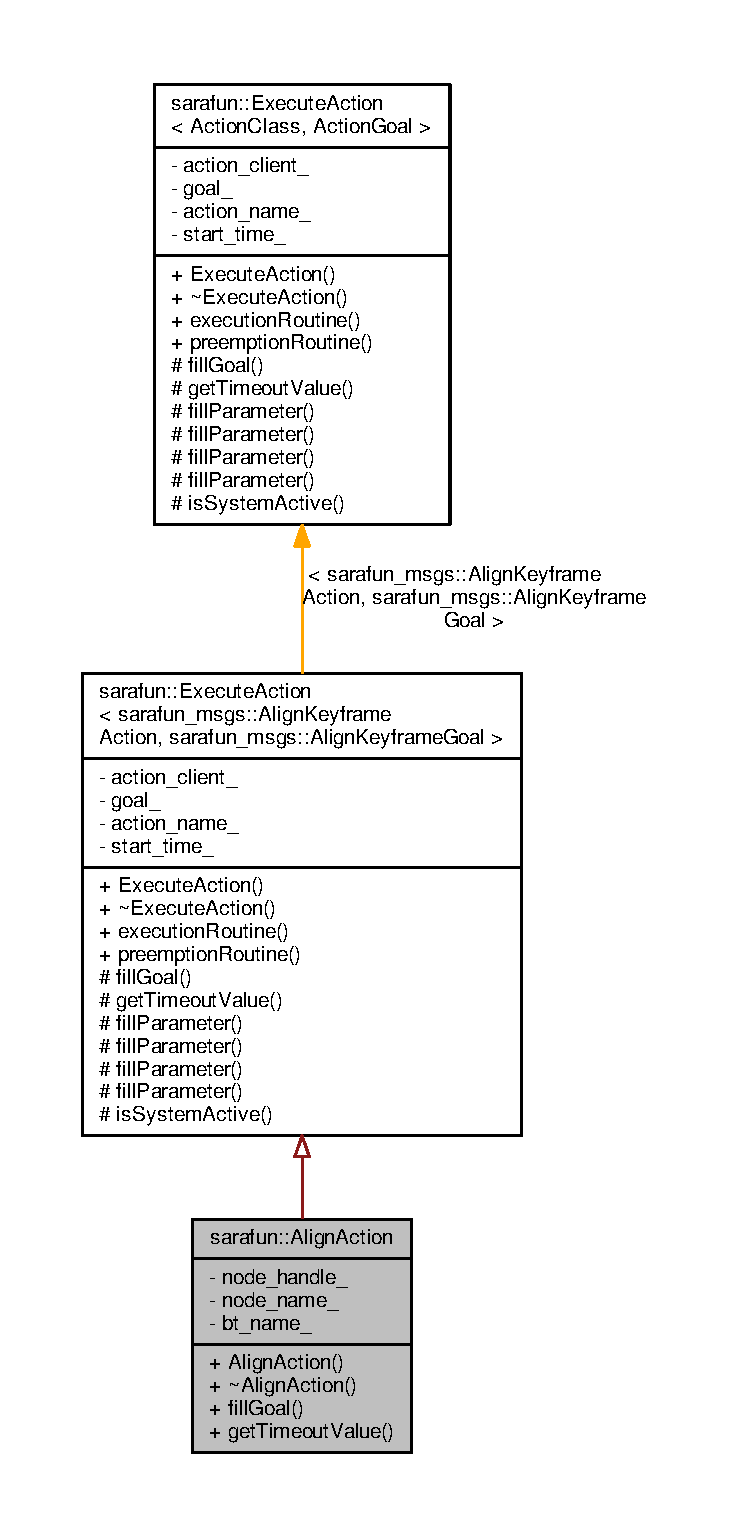
\includegraphics[height=550pt]{dc/d01/classsarafun_1_1AlignAction__inherit__graph}
\end{center}
\end{figure}


Collaboration diagram for sarafun\-:\-:Align\-Action\-:
\nopagebreak
\begin{figure}[H]
\begin{center}
\leavevmode
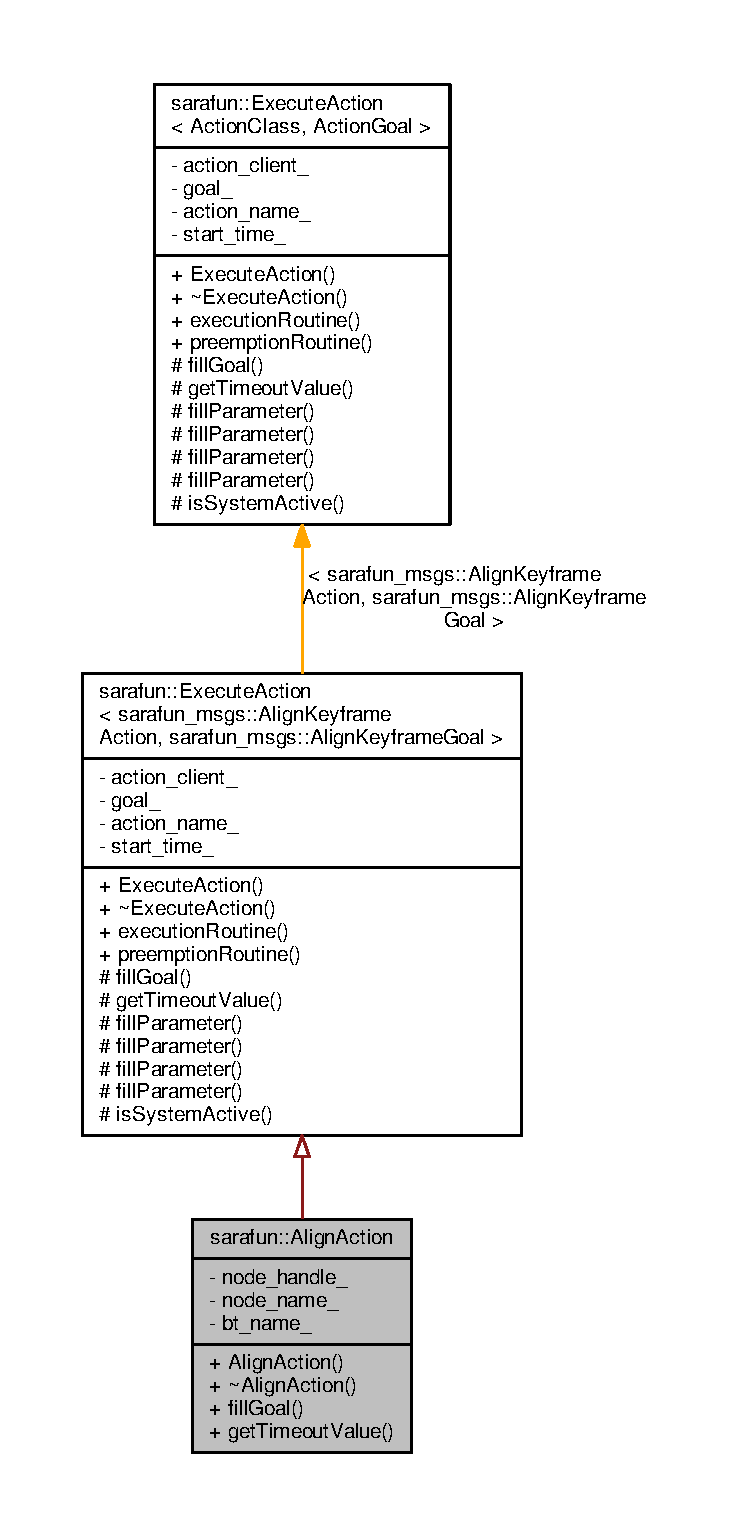
\includegraphics[height=550pt]{d2/d13/classsarafun_1_1AlignAction__coll__graph}
\end{center}
\end{figure}
\subsection*{Public Member Functions}
\begin{DoxyCompactItemize}
\item 
\hyperlink{classsarafun_1_1AlignAction_a013ed290585167a2693728565a764205_a013ed290585167a2693728565a764205}{Align\-Action} (std\-::string node\-\_\-name, std\-::string action\-\_\-name, std\-::string bt\-\_\-name)
\item 
\hyperlink{classsarafun_1_1AlignAction_a0fdb2f1de94801608024fb7dddd84f57_a0fdb2f1de94801608024fb7dddd84f57}{$\sim$\-Align\-Action} ()
\item 
bool \hyperlink{classsarafun_1_1AlignAction_ab92a62085ebd60438638b7b6c56da786_ab92a62085ebd60438638b7b6c56da786}{fill\-Goal} (sarafun\-\_\-msgs\-::\-Align\-Keyframe\-Goal \&goal)
\item 
double \hyperlink{classsarafun_1_1AlignAction_a9b9741ec3203bdc1b2e7b7cecc96e6ed_a9b9741ec3203bdc1b2e7b7cecc96e6ed}{get\-Timeout\-Value} ()
\end{DoxyCompactItemize}
\subsection*{Private Attributes}
\begin{DoxyCompactItemize}
\item 
ros\-::\-Node\-Handle \hyperlink{classsarafun_1_1AlignAction_acd1525d3ad1ad220e91af0c58802b6cf_acd1525d3ad1ad220e91af0c58802b6cf}{node\-\_\-handle\-\_\-}
\item 
std\-::string \hyperlink{classsarafun_1_1AlignAction_a4759b5ee1ef49d647eedcd8d04288799_a4759b5ee1ef49d647eedcd8d04288799}{node\-\_\-name\-\_\-}
\item 
std\-::string \hyperlink{classsarafun_1_1AlignAction_a832ecc3a169caf20ce7cb6f45d1551e3_a832ecc3a169caf20ce7cb6f45d1551e3}{bt\-\_\-name\-\_\-}
\end{DoxyCompactItemize}
\subsection*{Additional Inherited Members}


\subsection{Detailed Description}


Definition at line 9 of file Align\-Action.\-h.



\subsection{Constructor \& Destructor Documentation}
\hypertarget{classsarafun_1_1AlignAction_a013ed290585167a2693728565a764205_a013ed290585167a2693728565a764205}{\index{sarafun\-::\-Align\-Action@{sarafun\-::\-Align\-Action}!Align\-Action@{Align\-Action}}
\index{Align\-Action@{Align\-Action}!sarafun::AlignAction@{sarafun\-::\-Align\-Action}}
\subsubsection[{Align\-Action}]{\setlength{\rightskip}{0pt plus 5cm}sarafun\-::\-Align\-Action\-::\-Align\-Action (
\begin{DoxyParamCaption}
\item[{std\-::string}]{node\-\_\-name, }
\item[{std\-::string}]{action\-\_\-name, }
\item[{std\-::string}]{bt\-\_\-name}
\end{DoxyParamCaption}
)\hspace{0.3cm}{\ttfamily [inline]}}}\label{classsarafun_1_1AlignAction_a013ed290585167a2693728565a764205_a013ed290585167a2693728565a764205}


Definition at line 13 of file Align\-Action.\-h.



References node\-\_\-handle\-\_\-.

\hypertarget{classsarafun_1_1AlignAction_a0fdb2f1de94801608024fb7dddd84f57_a0fdb2f1de94801608024fb7dddd84f57}{\index{sarafun\-::\-Align\-Action@{sarafun\-::\-Align\-Action}!$\sim$\-Align\-Action@{$\sim$\-Align\-Action}}
\index{$\sim$\-Align\-Action@{$\sim$\-Align\-Action}!sarafun::AlignAction@{sarafun\-::\-Align\-Action}}
\subsubsection[{$\sim$\-Align\-Action}]{\setlength{\rightskip}{0pt plus 5cm}sarafun\-::\-Align\-Action\-::$\sim$\-Align\-Action (
\begin{DoxyParamCaption}
{}
\end{DoxyParamCaption}
)\hspace{0.3cm}{\ttfamily [inline]}}}\label{classsarafun_1_1AlignAction_a0fdb2f1de94801608024fb7dddd84f57_a0fdb2f1de94801608024fb7dddd84f57}


Definition at line 23 of file Align\-Action.\-h.



\subsection{Member Function Documentation}
\hypertarget{classsarafun_1_1AlignAction_ab92a62085ebd60438638b7b6c56da786_ab92a62085ebd60438638b7b6c56da786}{\index{sarafun\-::\-Align\-Action@{sarafun\-::\-Align\-Action}!fill\-Goal@{fill\-Goal}}
\index{fill\-Goal@{fill\-Goal}!sarafun::AlignAction@{sarafun\-::\-Align\-Action}}
\subsubsection[{fill\-Goal}]{\setlength{\rightskip}{0pt plus 5cm}bool sarafun\-::\-Align\-Action\-::fill\-Goal (
\begin{DoxyParamCaption}
\item[{sarafun\-\_\-msgs\-::\-Align\-Keyframe\-Goal \&}]{goal}
\end{DoxyParamCaption}
)\hspace{0.3cm}{\ttfamily [virtual]}}}\label{classsarafun_1_1AlignAction_ab92a62085ebd60438638b7b6c56da786_ab92a62085ebd60438638b7b6c56da786}
Fills in the goal for a particular action.


\begin{DoxyParams}{Parameters}
{\em goal} & The actionlib goal message of the externally implemented action. \\
\hline
\end{DoxyParams}
\begin{DoxyReturn}{Returns}
False in case of error, true otherwise. 
\end{DoxyReturn}


Implements \hyperlink{classsarafun_1_1ExecuteAction_a6dd9c0f013d15a17d7e7ce8dbe40a436_a6dd9c0f013d15a17d7e7ce8dbe40a436}{sarafun\-::\-Execute\-Action$<$ sarafun\-\_\-msgs\-::\-Align\-Keyframe\-Action, sarafun\-\_\-msgs\-::\-Align\-Keyframe\-Goal $>$}.



Definition at line 4 of file Align\-Action.\-cpp.



References sarafun\-::\-Execute\-Action$<$ sarafun\-\_\-msgs\-::\-Align\-Keyframe\-Action, sarafun\-\_\-msgs\-::\-Align\-Keyframe\-Goal $>$\-::fill\-Parameter().



Here is the call graph for this function\-:
\nopagebreak
\begin{figure}[H]
\begin{center}
\leavevmode
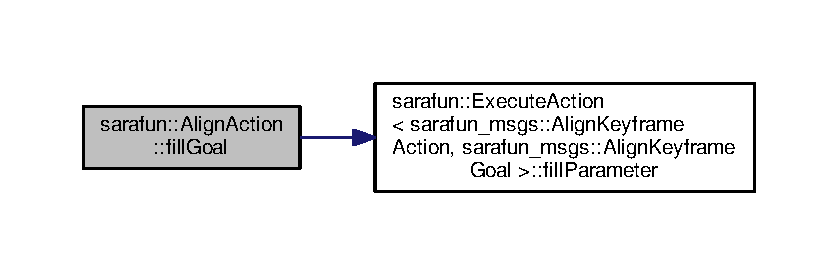
\includegraphics[width=350pt]{dc/df5/classsarafun_1_1AlignAction_ab92a62085ebd60438638b7b6c56da786_ab92a62085ebd60438638b7b6c56da786_cgraph}
\end{center}
\end{figure}


\hypertarget{classsarafun_1_1AlignAction_a9b9741ec3203bdc1b2e7b7cecc96e6ed_a9b9741ec3203bdc1b2e7b7cecc96e6ed}{\index{sarafun\-::\-Align\-Action@{sarafun\-::\-Align\-Action}!get\-Timeout\-Value@{get\-Timeout\-Value}}
\index{get\-Timeout\-Value@{get\-Timeout\-Value}!sarafun::AlignAction@{sarafun\-::\-Align\-Action}}
\subsubsection[{get\-Timeout\-Value}]{\setlength{\rightskip}{0pt plus 5cm}double sarafun\-::\-Align\-Action\-::get\-Timeout\-Value (
\begin{DoxyParamCaption}
{}
\end{DoxyParamCaption}
)\hspace{0.3cm}{\ttfamily [virtual]}}}\label{classsarafun_1_1AlignAction_a9b9741ec3203bdc1b2e7b7cecc96e6ed_a9b9741ec3203bdc1b2e7b7cecc96e6ed}
Provides the client with a timeout value for actionlib connections.

\begin{DoxyReturn}{Returns}
The timeout value (in seconds). 
\end{DoxyReturn}


Implements \hyperlink{classsarafun_1_1ExecuteAction_aba6cfa8a8ce19e735eb6394424df6d17_aba6cfa8a8ce19e735eb6394424df6d17}{sarafun\-::\-Execute\-Action$<$ sarafun\-\_\-msgs\-::\-Align\-Keyframe\-Action, sarafun\-\_\-msgs\-::\-Align\-Keyframe\-Goal $>$}.



Definition at line 13 of file Align\-Action.\-cpp.



References sarafun\-::\-Execute\-Action$<$ sarafun\-\_\-msgs\-::\-Align\-Keyframe\-Action, sarafun\-\_\-msgs\-::\-Align\-Keyframe\-Goal $>$\-::fill\-Parameter().



Here is the call graph for this function\-:
\nopagebreak
\begin{figure}[H]
\begin{center}
\leavevmode
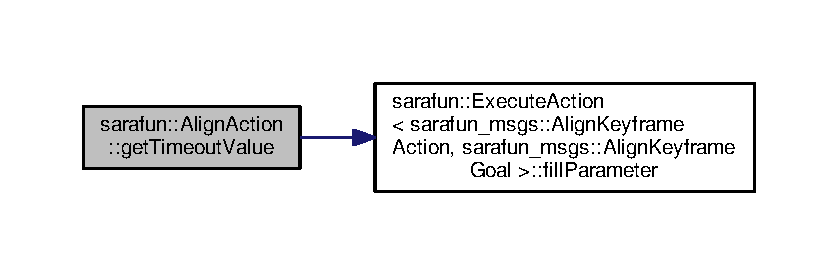
\includegraphics[width=350pt]{dc/df5/classsarafun_1_1AlignAction_a9b9741ec3203bdc1b2e7b7cecc96e6ed_a9b9741ec3203bdc1b2e7b7cecc96e6ed_cgraph}
\end{center}
\end{figure}




\subsection{Field Documentation}
\hypertarget{classsarafun_1_1AlignAction_a832ecc3a169caf20ce7cb6f45d1551e3_a832ecc3a169caf20ce7cb6f45d1551e3}{\index{sarafun\-::\-Align\-Action@{sarafun\-::\-Align\-Action}!bt\-\_\-name\-\_\-@{bt\-\_\-name\-\_\-}}
\index{bt\-\_\-name\-\_\-@{bt\-\_\-name\-\_\-}!sarafun::AlignAction@{sarafun\-::\-Align\-Action}}
\subsubsection[{bt\-\_\-name\-\_\-}]{\setlength{\rightskip}{0pt plus 5cm}std\-::string sarafun\-::\-Align\-Action\-::bt\-\_\-name\-\_\-\hspace{0.3cm}{\ttfamily [private]}}}\label{classsarafun_1_1AlignAction_a832ecc3a169caf20ce7cb6f45d1551e3_a832ecc3a169caf20ce7cb6f45d1551e3}


Definition at line 31 of file Align\-Action.\-h.

\hypertarget{classsarafun_1_1AlignAction_acd1525d3ad1ad220e91af0c58802b6cf_acd1525d3ad1ad220e91af0c58802b6cf}{\index{sarafun\-::\-Align\-Action@{sarafun\-::\-Align\-Action}!node\-\_\-handle\-\_\-@{node\-\_\-handle\-\_\-}}
\index{node\-\_\-handle\-\_\-@{node\-\_\-handle\-\_\-}!sarafun::AlignAction@{sarafun\-::\-Align\-Action}}
\subsubsection[{node\-\_\-handle\-\_\-}]{\setlength{\rightskip}{0pt plus 5cm}ros\-::\-Node\-Handle sarafun\-::\-Align\-Action\-::node\-\_\-handle\-\_\-\hspace{0.3cm}{\ttfamily [private]}}}\label{classsarafun_1_1AlignAction_acd1525d3ad1ad220e91af0c58802b6cf_acd1525d3ad1ad220e91af0c58802b6cf}


Definition at line 29 of file Align\-Action.\-h.



Referenced by Align\-Action().

\hypertarget{classsarafun_1_1AlignAction_a4759b5ee1ef49d647eedcd8d04288799_a4759b5ee1ef49d647eedcd8d04288799}{\index{sarafun\-::\-Align\-Action@{sarafun\-::\-Align\-Action}!node\-\_\-name\-\_\-@{node\-\_\-name\-\_\-}}
\index{node\-\_\-name\-\_\-@{node\-\_\-name\-\_\-}!sarafun::AlignAction@{sarafun\-::\-Align\-Action}}
\subsubsection[{node\-\_\-name\-\_\-}]{\setlength{\rightskip}{0pt plus 5cm}std\-::string sarafun\-::\-Align\-Action\-::node\-\_\-name\-\_\-\hspace{0.3cm}{\ttfamily [private]}}}\label{classsarafun_1_1AlignAction_a4759b5ee1ef49d647eedcd8d04288799_a4759b5ee1ef49d647eedcd8d04288799}


Definition at line 30 of file Align\-Action.\-h.



The documentation for this class was generated from the following files\-:\begin{DoxyCompactItemize}
\item 
Align\-Action.\-h\item 
Align\-Action.\-cpp\end{DoxyCompactItemize}

\hypertarget{classsarafun_1_1ApproachObjectsAction}{\section{sarafun\-:\-:Approach\-Objects\-Action Class Reference}
\label{classsarafun_1_1ApproachObjectsAction}\index{sarafun\-::\-Approach\-Objects\-Action@{sarafun\-::\-Approach\-Objects\-Action}}
}


{\ttfamily \#include $<$Approach\-Objects\-Action.\-h$>$}

Inheritance diagram for sarafun\-:\-:Approach\-Objects\-Action\-:\begin{figure}[H]
\begin{center}
\leavevmode
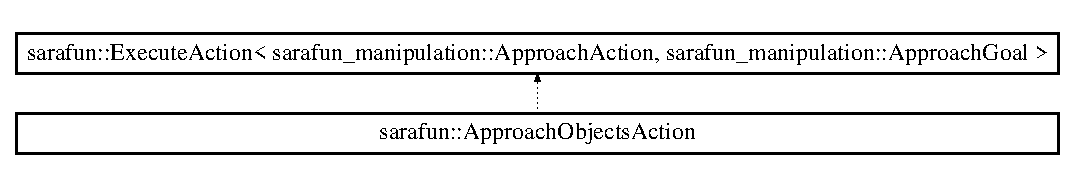
\includegraphics[height=1.839080cm]{classsarafun_1_1ApproachObjectsAction}
\end{center}
\end{figure}
\subsection*{Public Member Functions}
\begin{DoxyCompactItemize}
\item 
\hyperlink{classsarafun_1_1ApproachObjectsAction_ab0d857c262d75eeb85d8dc0e8f746f5f}{Approach\-Objects\-Action} (std\-::string node\-\_\-name, std\-::string action\-\_\-name, std\-::string bt\-\_\-name)
\item 
\hyperlink{classsarafun_1_1ApproachObjectsAction_adb6adaf7dae2e4addf53f47f07afd21e}{$\sim$\-Approach\-Objects\-Action} ()
\item 
bool \hyperlink{classsarafun_1_1ApproachObjectsAction_af5d216551122da780bc550daf4f1dca4}{fill\-Goal} (sarafun\-\_\-manipulation\-::\-Approach\-Goal \&goal)
\item 
double \hyperlink{classsarafun_1_1ApproachObjectsAction_a6852994a6e8a1edf9b2c24c91fd07df2}{get\-Timeout\-Value} ()
\end{DoxyCompactItemize}


\subsection{Constructor \& Destructor Documentation}
\hypertarget{classsarafun_1_1ApproachObjectsAction_ab0d857c262d75eeb85d8dc0e8f746f5f}{\index{sarafun\-::\-Approach\-Objects\-Action@{sarafun\-::\-Approach\-Objects\-Action}!Approach\-Objects\-Action@{Approach\-Objects\-Action}}
\index{Approach\-Objects\-Action@{Approach\-Objects\-Action}!sarafun::ApproachObjectsAction@{sarafun\-::\-Approach\-Objects\-Action}}
\subsubsection[{Approach\-Objects\-Action}]{\setlength{\rightskip}{0pt plus 5cm}sarafun\-::\-Approach\-Objects\-Action\-::\-Approach\-Objects\-Action (
\begin{DoxyParamCaption}
\item[{std\-::string}]{node\-\_\-name, }
\item[{std\-::string}]{action\-\_\-name, }
\item[{std\-::string}]{bt\-\_\-name}
\end{DoxyParamCaption}
)\hspace{0.3cm}{\ttfamily [inline]}}}\label{classsarafun_1_1ApproachObjectsAction_ab0d857c262d75eeb85d8dc0e8f746f5f}
\hypertarget{classsarafun_1_1ApproachObjectsAction_adb6adaf7dae2e4addf53f47f07afd21e}{\index{sarafun\-::\-Approach\-Objects\-Action@{sarafun\-::\-Approach\-Objects\-Action}!$\sim$\-Approach\-Objects\-Action@{$\sim$\-Approach\-Objects\-Action}}
\index{$\sim$\-Approach\-Objects\-Action@{$\sim$\-Approach\-Objects\-Action}!sarafun::ApproachObjectsAction@{sarafun\-::\-Approach\-Objects\-Action}}
\subsubsection[{$\sim$\-Approach\-Objects\-Action}]{\setlength{\rightskip}{0pt plus 5cm}sarafun\-::\-Approach\-Objects\-Action\-::$\sim$\-Approach\-Objects\-Action (
\begin{DoxyParamCaption}
{}
\end{DoxyParamCaption}
)\hspace{0.3cm}{\ttfamily [inline]}}}\label{classsarafun_1_1ApproachObjectsAction_adb6adaf7dae2e4addf53f47f07afd21e}


\subsection{Member Function Documentation}
\hypertarget{classsarafun_1_1ApproachObjectsAction_af5d216551122da780bc550daf4f1dca4}{\index{sarafun\-::\-Approach\-Objects\-Action@{sarafun\-::\-Approach\-Objects\-Action}!fill\-Goal@{fill\-Goal}}
\index{fill\-Goal@{fill\-Goal}!sarafun::ApproachObjectsAction@{sarafun\-::\-Approach\-Objects\-Action}}
\subsubsection[{fill\-Goal}]{\setlength{\rightskip}{0pt plus 5cm}bool sarafun\-::\-Approach\-Objects\-Action\-::fill\-Goal (
\begin{DoxyParamCaption}
\item[{sarafun\-\_\-manipulation\-::\-Approach\-Goal \&}]{goal}
\end{DoxyParamCaption}
)\hspace{0.3cm}{\ttfamily [virtual]}}}\label{classsarafun_1_1ApproachObjectsAction_af5d216551122da780bc550daf4f1dca4}
Fills in the goal for a particular action.


\begin{DoxyParams}{Parameters}
{\em goal} & The actionlib goal message of the externally implemented action. \\
\hline
\end{DoxyParams}
\begin{DoxyReturn}{Returns}
False in case of error, true otherwise. 
\end{DoxyReturn}


Implements \hyperlink{classsarafun_1_1ExecuteAction_a6dd9c0f013d15a17d7e7ce8dbe40a436}{sarafun\-::\-Execute\-Action$<$ sarafun\-\_\-manipulation\-::\-Approach\-Action, sarafun\-\_\-manipulation\-::\-Approach\-Goal $>$}.

\hypertarget{classsarafun_1_1ApproachObjectsAction_a6852994a6e8a1edf9b2c24c91fd07df2}{\index{sarafun\-::\-Approach\-Objects\-Action@{sarafun\-::\-Approach\-Objects\-Action}!get\-Timeout\-Value@{get\-Timeout\-Value}}
\index{get\-Timeout\-Value@{get\-Timeout\-Value}!sarafun::ApproachObjectsAction@{sarafun\-::\-Approach\-Objects\-Action}}
\subsubsection[{get\-Timeout\-Value}]{\setlength{\rightskip}{0pt plus 5cm}double sarafun\-::\-Approach\-Objects\-Action\-::get\-Timeout\-Value (
\begin{DoxyParamCaption}
{}
\end{DoxyParamCaption}
)\hspace{0.3cm}{\ttfamily [virtual]}}}\label{classsarafun_1_1ApproachObjectsAction_a6852994a6e8a1edf9b2c24c91fd07df2}
Provides the client with a timeout value for actionlib connections.

\begin{DoxyReturn}{Returns}
The timeout value (in seconds). 
\end{DoxyReturn}


Implements \hyperlink{classsarafun_1_1ExecuteAction_aba6cfa8a8ce19e735eb6394424df6d17}{sarafun\-::\-Execute\-Action$<$ sarafun\-\_\-manipulation\-::\-Approach\-Action, sarafun\-\_\-manipulation\-::\-Approach\-Goal $>$}.



The documentation for this class was generated from the following files\-:\begin{DoxyCompactItemize}
\item 
sarafun\-\_\-tree/include/sarafun\-\_\-tree/demo\-\_\-bt\-\_\-nodes/\hyperlink{ApproachObjectsAction_8h}{Approach\-Objects\-Action.\-h}\item 
sarafun\-\_\-tree/src/demo\-\_\-bt\-\_\-nodes/\hyperlink{ApproachObjectsAction_8cpp}{Approach\-Objects\-Action.\-cpp}\end{DoxyCompactItemize}

\hypertarget{classsarafun_1_1AssembledAction}{\section{sarafun\-:\-:Assembled\-Action Class Reference}
\label{classsarafun_1_1AssembledAction}\index{sarafun\-::\-Assembled\-Action@{sarafun\-::\-Assembled\-Action}}
}


{\ttfamily \#include $<$Assembled\-Action.\-h$>$}



Inheritance diagram for sarafun\-:\-:Assembled\-Action\-:
\nopagebreak
\begin{figure}[H]
\begin{center}
\leavevmode
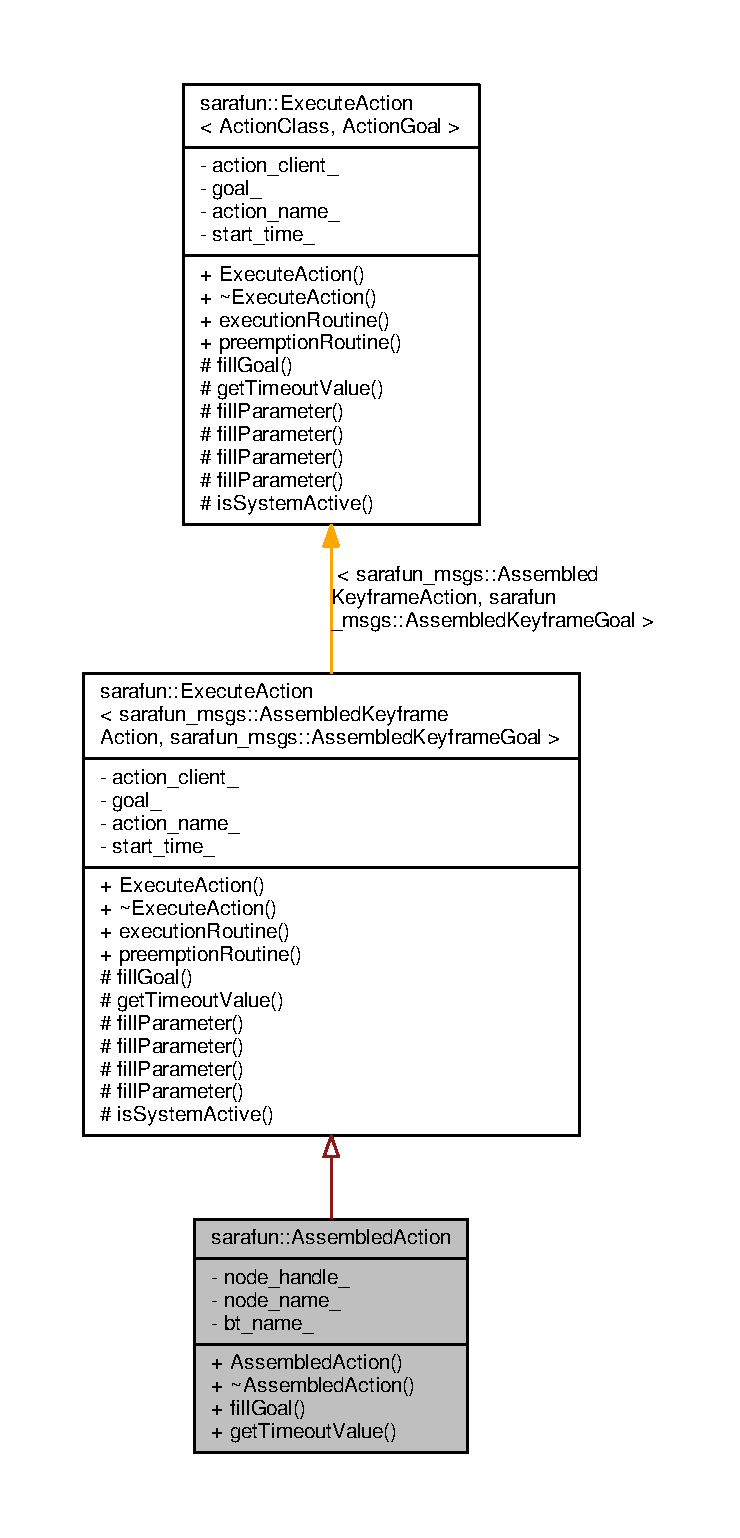
\includegraphics[height=550pt]{d9/d73/classsarafun_1_1AssembledAction__inherit__graph}
\end{center}
\end{figure}


Collaboration diagram for sarafun\-:\-:Assembled\-Action\-:
\nopagebreak
\begin{figure}[H]
\begin{center}
\leavevmode
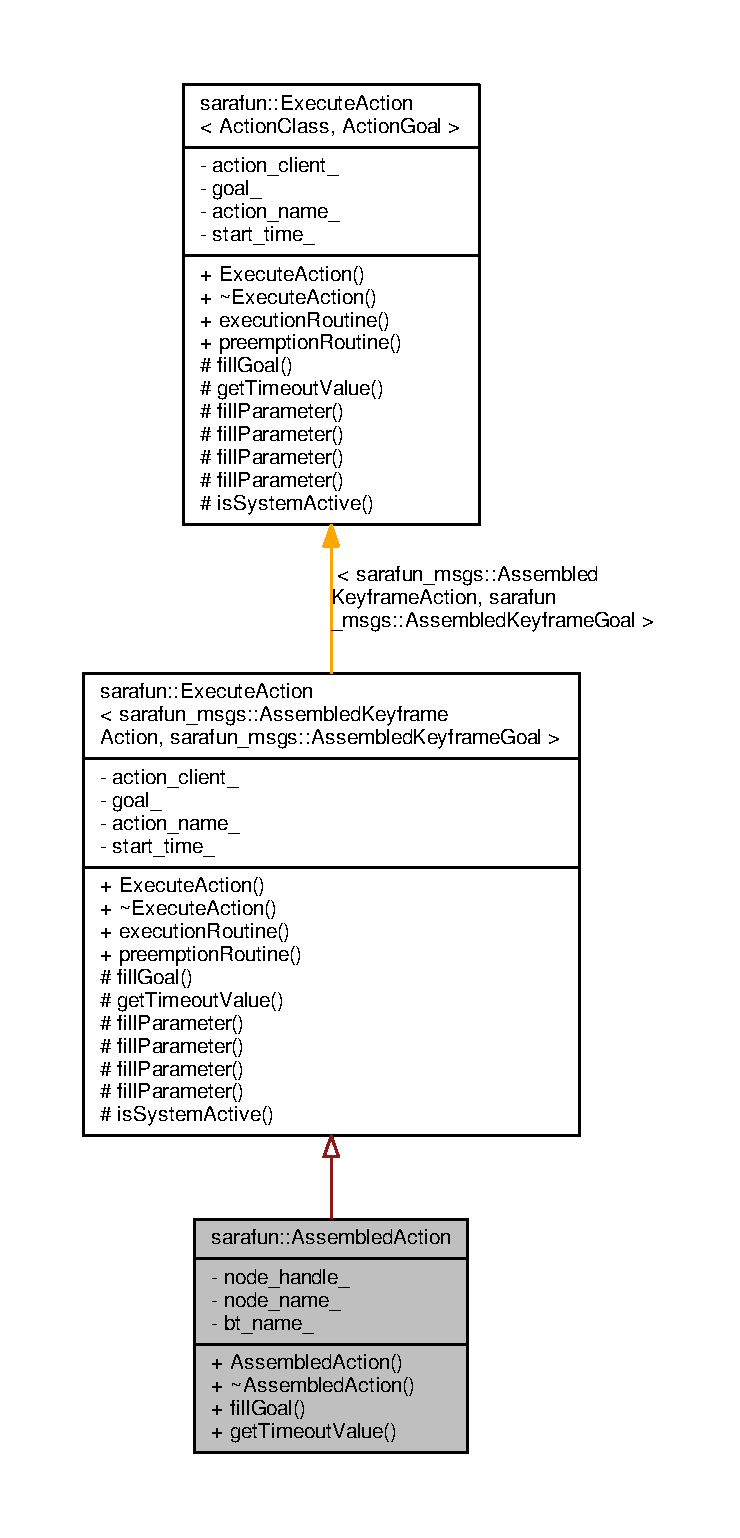
\includegraphics[height=550pt]{d7/df2/classsarafun_1_1AssembledAction__coll__graph}
\end{center}
\end{figure}
\subsection*{Public Member Functions}
\begin{DoxyCompactItemize}
\item 
\hyperlink{classsarafun_1_1AssembledAction_a0207a1b903e0189627087d7ed71bc130_a0207a1b903e0189627087d7ed71bc130}{Assembled\-Action} (std\-::string node\-\_\-name, std\-::string action\-\_\-name, std\-::string bt\-\_\-name)
\item 
\hyperlink{classsarafun_1_1AssembledAction_a8d290f1548b55bca1995df599272fc2f_a8d290f1548b55bca1995df599272fc2f}{$\sim$\-Assembled\-Action} ()
\item 
bool \hyperlink{classsarafun_1_1AssembledAction_a094a5cfde4d6bb6d024256834e771a39_a094a5cfde4d6bb6d024256834e771a39}{fill\-Goal} (sarafun\-\_\-msgs\-::\-Assembled\-Keyframe\-Goal \&goal)
\item 
double \hyperlink{classsarafun_1_1AssembledAction_ade9095a291dce652339238d137419b49_ade9095a291dce652339238d137419b49}{get\-Timeout\-Value} ()
\end{DoxyCompactItemize}
\subsection*{Private Attributes}
\begin{DoxyCompactItemize}
\item 
ros\-::\-Node\-Handle \hyperlink{classsarafun_1_1AssembledAction_ae97c585b30dd24e64cc08f78c08e52c5_ae97c585b30dd24e64cc08f78c08e52c5}{node\-\_\-handle\-\_\-}
\item 
std\-::string \hyperlink{classsarafun_1_1AssembledAction_a693b73bd880c4b9c193dea5ab62c1df8_a693b73bd880c4b9c193dea5ab62c1df8}{node\-\_\-name\-\_\-}
\item 
std\-::string \hyperlink{classsarafun_1_1AssembledAction_a4dae92c3c98d924c35f9cda69ede136d_a4dae92c3c98d924c35f9cda69ede136d}{bt\-\_\-name\-\_\-}
\end{DoxyCompactItemize}
\subsection*{Additional Inherited Members}


\subsection{Detailed Description}


Definition at line 9 of file Assembled\-Action.\-h.



\subsection{Constructor \& Destructor Documentation}
\hypertarget{classsarafun_1_1AssembledAction_a0207a1b903e0189627087d7ed71bc130_a0207a1b903e0189627087d7ed71bc130}{\index{sarafun\-::\-Assembled\-Action@{sarafun\-::\-Assembled\-Action}!Assembled\-Action@{Assembled\-Action}}
\index{Assembled\-Action@{Assembled\-Action}!sarafun::AssembledAction@{sarafun\-::\-Assembled\-Action}}
\subsubsection[{Assembled\-Action}]{\setlength{\rightskip}{0pt plus 5cm}sarafun\-::\-Assembled\-Action\-::\-Assembled\-Action (
\begin{DoxyParamCaption}
\item[{std\-::string}]{node\-\_\-name, }
\item[{std\-::string}]{action\-\_\-name, }
\item[{std\-::string}]{bt\-\_\-name}
\end{DoxyParamCaption}
)\hspace{0.3cm}{\ttfamily [inline]}}}\label{classsarafun_1_1AssembledAction_a0207a1b903e0189627087d7ed71bc130_a0207a1b903e0189627087d7ed71bc130}


Definition at line 13 of file Assembled\-Action.\-h.



References node\-\_\-handle\-\_\-.

\hypertarget{classsarafun_1_1AssembledAction_a8d290f1548b55bca1995df599272fc2f_a8d290f1548b55bca1995df599272fc2f}{\index{sarafun\-::\-Assembled\-Action@{sarafun\-::\-Assembled\-Action}!$\sim$\-Assembled\-Action@{$\sim$\-Assembled\-Action}}
\index{$\sim$\-Assembled\-Action@{$\sim$\-Assembled\-Action}!sarafun::AssembledAction@{sarafun\-::\-Assembled\-Action}}
\subsubsection[{$\sim$\-Assembled\-Action}]{\setlength{\rightskip}{0pt plus 5cm}sarafun\-::\-Assembled\-Action\-::$\sim$\-Assembled\-Action (
\begin{DoxyParamCaption}
{}
\end{DoxyParamCaption}
)\hspace{0.3cm}{\ttfamily [inline]}}}\label{classsarafun_1_1AssembledAction_a8d290f1548b55bca1995df599272fc2f_a8d290f1548b55bca1995df599272fc2f}


Definition at line 23 of file Assembled\-Action.\-h.



\subsection{Member Function Documentation}
\hypertarget{classsarafun_1_1AssembledAction_a094a5cfde4d6bb6d024256834e771a39_a094a5cfde4d6bb6d024256834e771a39}{\index{sarafun\-::\-Assembled\-Action@{sarafun\-::\-Assembled\-Action}!fill\-Goal@{fill\-Goal}}
\index{fill\-Goal@{fill\-Goal}!sarafun::AssembledAction@{sarafun\-::\-Assembled\-Action}}
\subsubsection[{fill\-Goal}]{\setlength{\rightskip}{0pt plus 5cm}bool sarafun\-::\-Assembled\-Action\-::fill\-Goal (
\begin{DoxyParamCaption}
\item[{sarafun\-\_\-msgs\-::\-Assembled\-Keyframe\-Goal \&}]{goal}
\end{DoxyParamCaption}
)\hspace{0.3cm}{\ttfamily [virtual]}}}\label{classsarafun_1_1AssembledAction_a094a5cfde4d6bb6d024256834e771a39_a094a5cfde4d6bb6d024256834e771a39}
Fills in the goal for a particular action.


\begin{DoxyParams}{Parameters}
{\em goal} & The actionlib goal message of the externally implemented action. \\
\hline
\end{DoxyParams}
\begin{DoxyReturn}{Returns}
False in case of error, true otherwise. 
\end{DoxyReturn}


Implements \hyperlink{classsarafun_1_1ExecuteAction_a6dd9c0f013d15a17d7e7ce8dbe40a436_a6dd9c0f013d15a17d7e7ce8dbe40a436}{sarafun\-::\-Execute\-Action$<$ sarafun\-\_\-msgs\-::\-Assembled\-Keyframe\-Action, sarafun\-\_\-msgs\-::\-Assembled\-Keyframe\-Goal $>$}.



Definition at line 4 of file Assembled\-Action.\-cpp.



References sarafun\-::\-Execute\-Action$<$ sarafun\-\_\-msgs\-::\-Assembled\-Keyframe\-Action, sarafun\-\_\-msgs\-::\-Assembled\-Keyframe\-Goal $>$\-::fill\-Parameter().



Here is the call graph for this function\-:
\nopagebreak
\begin{figure}[H]
\begin{center}
\leavevmode
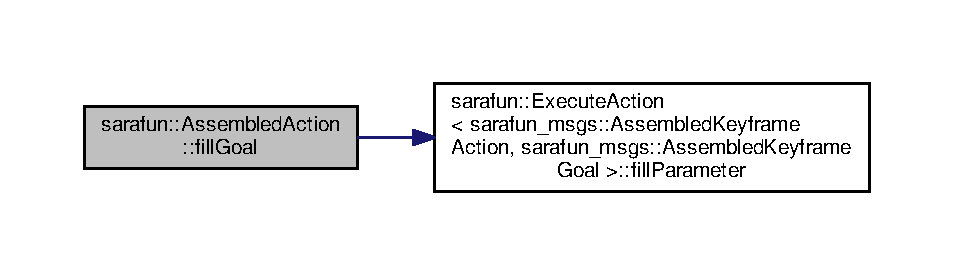
\includegraphics[width=350pt]{dc/d58/classsarafun_1_1AssembledAction_a094a5cfde4d6bb6d024256834e771a39_a094a5cfde4d6bb6d024256834e771a39_cgraph}
\end{center}
\end{figure}


\hypertarget{classsarafun_1_1AssembledAction_ade9095a291dce652339238d137419b49_ade9095a291dce652339238d137419b49}{\index{sarafun\-::\-Assembled\-Action@{sarafun\-::\-Assembled\-Action}!get\-Timeout\-Value@{get\-Timeout\-Value}}
\index{get\-Timeout\-Value@{get\-Timeout\-Value}!sarafun::AssembledAction@{sarafun\-::\-Assembled\-Action}}
\subsubsection[{get\-Timeout\-Value}]{\setlength{\rightskip}{0pt plus 5cm}double sarafun\-::\-Assembled\-Action\-::get\-Timeout\-Value (
\begin{DoxyParamCaption}
{}
\end{DoxyParamCaption}
)\hspace{0.3cm}{\ttfamily [virtual]}}}\label{classsarafun_1_1AssembledAction_ade9095a291dce652339238d137419b49_ade9095a291dce652339238d137419b49}
Provides the client with a timeout value for actionlib connections.

\begin{DoxyReturn}{Returns}
The timeout value (in seconds). 
\end{DoxyReturn}


Implements \hyperlink{classsarafun_1_1ExecuteAction_aba6cfa8a8ce19e735eb6394424df6d17_aba6cfa8a8ce19e735eb6394424df6d17}{sarafun\-::\-Execute\-Action$<$ sarafun\-\_\-msgs\-::\-Assembled\-Keyframe\-Action, sarafun\-\_\-msgs\-::\-Assembled\-Keyframe\-Goal $>$}.



Definition at line 13 of file Assembled\-Action.\-cpp.



References sarafun\-::\-Execute\-Action$<$ sarafun\-\_\-msgs\-::\-Assembled\-Keyframe\-Action, sarafun\-\_\-msgs\-::\-Assembled\-Keyframe\-Goal $>$\-::fill\-Parameter().



Here is the call graph for this function\-:
\nopagebreak
\begin{figure}[H]
\begin{center}
\leavevmode
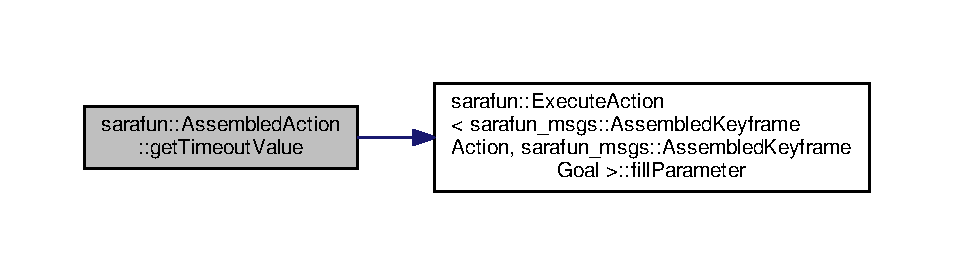
\includegraphics[width=350pt]{dc/d58/classsarafun_1_1AssembledAction_ade9095a291dce652339238d137419b49_ade9095a291dce652339238d137419b49_cgraph}
\end{center}
\end{figure}




\subsection{Field Documentation}
\hypertarget{classsarafun_1_1AssembledAction_a4dae92c3c98d924c35f9cda69ede136d_a4dae92c3c98d924c35f9cda69ede136d}{\index{sarafun\-::\-Assembled\-Action@{sarafun\-::\-Assembled\-Action}!bt\-\_\-name\-\_\-@{bt\-\_\-name\-\_\-}}
\index{bt\-\_\-name\-\_\-@{bt\-\_\-name\-\_\-}!sarafun::AssembledAction@{sarafun\-::\-Assembled\-Action}}
\subsubsection[{bt\-\_\-name\-\_\-}]{\setlength{\rightskip}{0pt plus 5cm}std\-::string sarafun\-::\-Assembled\-Action\-::bt\-\_\-name\-\_\-\hspace{0.3cm}{\ttfamily [private]}}}\label{classsarafun_1_1AssembledAction_a4dae92c3c98d924c35f9cda69ede136d_a4dae92c3c98d924c35f9cda69ede136d}


Definition at line 31 of file Assembled\-Action.\-h.

\hypertarget{classsarafun_1_1AssembledAction_ae97c585b30dd24e64cc08f78c08e52c5_ae97c585b30dd24e64cc08f78c08e52c5}{\index{sarafun\-::\-Assembled\-Action@{sarafun\-::\-Assembled\-Action}!node\-\_\-handle\-\_\-@{node\-\_\-handle\-\_\-}}
\index{node\-\_\-handle\-\_\-@{node\-\_\-handle\-\_\-}!sarafun::AssembledAction@{sarafun\-::\-Assembled\-Action}}
\subsubsection[{node\-\_\-handle\-\_\-}]{\setlength{\rightskip}{0pt plus 5cm}ros\-::\-Node\-Handle sarafun\-::\-Assembled\-Action\-::node\-\_\-handle\-\_\-\hspace{0.3cm}{\ttfamily [private]}}}\label{classsarafun_1_1AssembledAction_ae97c585b30dd24e64cc08f78c08e52c5_ae97c585b30dd24e64cc08f78c08e52c5}


Definition at line 29 of file Assembled\-Action.\-h.



Referenced by Assembled\-Action().

\hypertarget{classsarafun_1_1AssembledAction_a693b73bd880c4b9c193dea5ab62c1df8_a693b73bd880c4b9c193dea5ab62c1df8}{\index{sarafun\-::\-Assembled\-Action@{sarafun\-::\-Assembled\-Action}!node\-\_\-name\-\_\-@{node\-\_\-name\-\_\-}}
\index{node\-\_\-name\-\_\-@{node\-\_\-name\-\_\-}!sarafun::AssembledAction@{sarafun\-::\-Assembled\-Action}}
\subsubsection[{node\-\_\-name\-\_\-}]{\setlength{\rightskip}{0pt plus 5cm}std\-::string sarafun\-::\-Assembled\-Action\-::node\-\_\-name\-\_\-\hspace{0.3cm}{\ttfamily [private]}}}\label{classsarafun_1_1AssembledAction_a693b73bd880c4b9c193dea5ab62c1df8_a693b73bd880c4b9c193dea5ab62c1df8}


Definition at line 30 of file Assembled\-Action.\-h.



The documentation for this class was generated from the following files\-:\begin{DoxyCompactItemize}
\item 
Assembled\-Action.\-h\item 
Assembled\-Action.\-cpp\end{DoxyCompactItemize}

\hypertarget{classnlohmann_1_1basic__json}{\section{nlohmann\-:\-:basic\-\_\-json$<$ Object\-Type, Array\-Type, String\-Type, Boolean\-Type, Number\-Integer\-Type, Number\-Unsigned\-Type, Number\-Float\-Type, Allocator\-Type $>$ Class Template Reference}
\label{classnlohmann_1_1basic__json}\index{nlohmann\-::basic\-\_\-json$<$ Object\-Type, Array\-Type, String\-Type, Boolean\-Type, Number\-Integer\-Type, Number\-Unsigned\-Type, Number\-Float\-Type, Allocator\-Type $>$@{nlohmann\-::basic\-\_\-json$<$ Object\-Type, Array\-Type, String\-Type, Boolean\-Type, Number\-Integer\-Type, Number\-Unsigned\-Type, Number\-Float\-Type, Allocator\-Type $>$}}
}


a class to store J\-S\-O\-N values  




{\ttfamily \#include $<$json.\-hpp$>$}

\subsection*{Data Structures}
\begin{DoxyCompactItemize}
\item 
class \hyperlink{classnlohmann_1_1basic__json_1_1const__iterator}{const\-\_\-iterator}
\begin{DoxyCompactList}\small\item\em a const random access iterator for the \hyperlink{classnlohmann_1_1basic__json}{basic\-\_\-json} class \end{DoxyCompactList}\item 
struct \hyperlink{structnlohmann_1_1basic__json_1_1internal__iterator}{internal\-\_\-iterator}
\begin{DoxyCompactList}\small\item\em an iterator value \end{DoxyCompactList}\item 
class \hyperlink{classnlohmann_1_1basic__json_1_1iteration__proxy}{iteration\-\_\-proxy}
\begin{DoxyCompactList}\small\item\em proxy class for the iterator\-\_\-wrapper functions \end{DoxyCompactList}\item 
class \hyperlink{classnlohmann_1_1basic__json_1_1iterator}{iterator}
\begin{DoxyCompactList}\small\item\em a mutable random access iterator for the \hyperlink{classnlohmann_1_1basic__json}{basic\-\_\-json} class \end{DoxyCompactList}\item 
class \hyperlink{classnlohmann_1_1basic__json_1_1json__pointer}{json\-\_\-pointer}
\begin{DoxyCompactList}\small\item\em J\-S\-O\-N Pointer. \end{DoxyCompactList}\item 
class \hyperlink{classnlohmann_1_1basic__json_1_1json__reverse__iterator}{json\-\_\-reverse\-\_\-iterator}
\begin{DoxyCompactList}\small\item\em a template for a reverse iterator class \end{DoxyCompactList}\item 
union \hyperlink{unionnlohmann_1_1basic__json_1_1json__value}{json\-\_\-value}
\begin{DoxyCompactList}\small\item\em a J\-S\-O\-N value \end{DoxyCompactList}\item 
class \hyperlink{classnlohmann_1_1basic__json_1_1lexer}{lexer}
\begin{DoxyCompactList}\small\item\em lexical analysis \end{DoxyCompactList}\item 
class \hyperlink{classnlohmann_1_1basic__json_1_1parser}{parser}
\begin{DoxyCompactList}\small\item\em syntax analysis \end{DoxyCompactList}\item 
class \hyperlink{classnlohmann_1_1basic__json_1_1primitive__iterator__t}{primitive\-\_\-iterator\-\_\-t}
\begin{DoxyCompactList}\small\item\em an iterator for primitive J\-S\-O\-N types \end{DoxyCompactList}\item 
union \hyperlink{unionnlohmann_1_1basic__json_1_1type__data__t}{type\-\_\-data\-\_\-t}
\begin{DoxyCompactList}\small\item\em a type to hold J\-S\-O\-N type information \end{DoxyCompactList}\end{DoxyCompactItemize}
\subsection*{Public Types}
\begin{DoxyCompactItemize}
\item 
enum \hyperlink{classnlohmann_1_1basic__json_a231b02148577b69a154b2ce2c87a5522_a231b02148577b69a154b2ce2c87a5522}{value\-\_\-t} \-: uint8\-\_\-t \{ \\*
\hyperlink{classnlohmann_1_1basic__json_a231b02148577b69a154b2ce2c87a5522_a231b02148577b69a154b2ce2c87a5522a37a6259cc0c1dae299a7866489dff0bd}{value\-\_\-t\-::null}, 
\hyperlink{classnlohmann_1_1basic__json_a231b02148577b69a154b2ce2c87a5522_a231b02148577b69a154b2ce2c87a5522aa8cfde6331bd59eb2ac96f8911c4b666}{value\-\_\-t\-::object}, 
\hyperlink{classnlohmann_1_1basic__json_a231b02148577b69a154b2ce2c87a5522_a231b02148577b69a154b2ce2c87a5522af1f713c9e000f5d3f280adbd124df4f5}{value\-\_\-t\-::array}, 
\hyperlink{classnlohmann_1_1basic__json_a231b02148577b69a154b2ce2c87a5522_a231b02148577b69a154b2ce2c87a5522ab45cffe084dd3d20d928bee85e7b0f21}{value\-\_\-t\-::string}, 
\\*
\hyperlink{classnlohmann_1_1basic__json_a231b02148577b69a154b2ce2c87a5522_a231b02148577b69a154b2ce2c87a5522a84e2c64f38f78ba3ea5c905ab5a2da27}{value\-\_\-t\-::boolean}, 
\hyperlink{classnlohmann_1_1basic__json_a231b02148577b69a154b2ce2c87a5522_a231b02148577b69a154b2ce2c87a5522a5763da164f8659d94a56e29df64b4bcc}{value\-\_\-t\-::number\-\_\-integer}, 
\hyperlink{classnlohmann_1_1basic__json_a231b02148577b69a154b2ce2c87a5522_a231b02148577b69a154b2ce2c87a5522adce7cc8ec29055c4158828921f2f265e}{value\-\_\-t\-::number\-\_\-unsigned}, 
\hyperlink{classnlohmann_1_1basic__json_a231b02148577b69a154b2ce2c87a5522_a231b02148577b69a154b2ce2c87a5522ad9966ecb59667235a57b4b999a649eef}{value\-\_\-t\-::number\-\_\-float}, 
\\*
\hyperlink{classnlohmann_1_1basic__json_a231b02148577b69a154b2ce2c87a5522_a231b02148577b69a154b2ce2c87a5522a94708897ec9db8647dfe695714c98e46}{value\-\_\-t\-::discarded}, 
\hyperlink{classnlohmann_1_1basic__json_a231b02148577b69a154b2ce2c87a5522_a231b02148577b69a154b2ce2c87a5522a37a6259cc0c1dae299a7866489dff0bd}{value\-\_\-t\-::null}, 
\hyperlink{classnlohmann_1_1basic__json_a231b02148577b69a154b2ce2c87a5522_a231b02148577b69a154b2ce2c87a5522aa8cfde6331bd59eb2ac96f8911c4b666}{value\-\_\-t\-::object}, 
\hyperlink{classnlohmann_1_1basic__json_a231b02148577b69a154b2ce2c87a5522_a231b02148577b69a154b2ce2c87a5522af1f713c9e000f5d3f280adbd124df4f5}{value\-\_\-t\-::array}, 
\\*
\hyperlink{classnlohmann_1_1basic__json_a231b02148577b69a154b2ce2c87a5522_a231b02148577b69a154b2ce2c87a5522ab45cffe084dd3d20d928bee85e7b0f21}{value\-\_\-t\-::string}, 
\hyperlink{classnlohmann_1_1basic__json_a231b02148577b69a154b2ce2c87a5522_a231b02148577b69a154b2ce2c87a5522a84e2c64f38f78ba3ea5c905ab5a2da27}{value\-\_\-t\-::boolean}, 
\hyperlink{classnlohmann_1_1basic__json_a231b02148577b69a154b2ce2c87a5522_a231b02148577b69a154b2ce2c87a5522a5763da164f8659d94a56e29df64b4bcc}{value\-\_\-t\-::number\-\_\-integer}, 
\hyperlink{classnlohmann_1_1basic__json_a231b02148577b69a154b2ce2c87a5522_a231b02148577b69a154b2ce2c87a5522adce7cc8ec29055c4158828921f2f265e}{value\-\_\-t\-::number\-\_\-unsigned}, 
\\*
\hyperlink{classnlohmann_1_1basic__json_a231b02148577b69a154b2ce2c87a5522_a231b02148577b69a154b2ce2c87a5522ad9966ecb59667235a57b4b999a649eef}{value\-\_\-t\-::number\-\_\-float}, 
\hyperlink{classnlohmann_1_1basic__json_a231b02148577b69a154b2ce2c87a5522_a231b02148577b69a154b2ce2c87a5522a94708897ec9db8647dfe695714c98e46}{value\-\_\-t\-::discarded}
 \}
\begin{DoxyCompactList}\small\item\em the J\-S\-O\-N type enumeration \end{DoxyCompactList}\item 
enum \hyperlink{classnlohmann_1_1basic__json_aea1c863b719b4ca5b77188c171bbfafe_aea1c863b719b4ca5b77188c171bbfafe}{parse\-\_\-event\-\_\-t} \-: uint8\-\_\-t \{ \\*
\hyperlink{classnlohmann_1_1basic__json_aea1c863b719b4ca5b77188c171bbfafe_aea1c863b719b4ca5b77188c171bbfafeae73f17027cb0acbb537f29d0a6944b26}{parse\-\_\-event\-\_\-t\-::object\-\_\-start}, 
\hyperlink{classnlohmann_1_1basic__json_aea1c863b719b4ca5b77188c171bbfafe_aea1c863b719b4ca5b77188c171bbfafeaf63e2a2468a37aa4f394fcc3bcb8249c}{parse\-\_\-event\-\_\-t\-::object\-\_\-end}, 
\hyperlink{classnlohmann_1_1basic__json_aea1c863b719b4ca5b77188c171bbfafe_aea1c863b719b4ca5b77188c171bbfafeaa4388a3d92419edbb1c6efd4d52461f3}{parse\-\_\-event\-\_\-t\-::array\-\_\-start}, 
\hyperlink{classnlohmann_1_1basic__json_aea1c863b719b4ca5b77188c171bbfafe_aea1c863b719b4ca5b77188c171bbfafea49642fb732aa2e112188fba1f9d3ef7f}{parse\-\_\-event\-\_\-t\-::array\-\_\-end}, 
\\*
\hyperlink{classnlohmann_1_1basic__json_aea1c863b719b4ca5b77188c171bbfafe_aea1c863b719b4ca5b77188c171bbfafea3c6e0b8a9c15224a8228b9a98ca1531d}{parse\-\_\-event\-\_\-t\-::key}, 
\hyperlink{classnlohmann_1_1basic__json_aea1c863b719b4ca5b77188c171bbfafe_aea1c863b719b4ca5b77188c171bbfafea2063c1608d6e0baf80249c42e2be5804}{parse\-\_\-event\-\_\-t\-::value}, 
\hyperlink{classnlohmann_1_1basic__json_aea1c863b719b4ca5b77188c171bbfafe_aea1c863b719b4ca5b77188c171bbfafeae73f17027cb0acbb537f29d0a6944b26}{parse\-\_\-event\-\_\-t\-::object\-\_\-start}, 
\hyperlink{classnlohmann_1_1basic__json_aea1c863b719b4ca5b77188c171bbfafe_aea1c863b719b4ca5b77188c171bbfafeaf63e2a2468a37aa4f394fcc3bcb8249c}{parse\-\_\-event\-\_\-t\-::object\-\_\-end}, 
\\*
\hyperlink{classnlohmann_1_1basic__json_aea1c863b719b4ca5b77188c171bbfafe_aea1c863b719b4ca5b77188c171bbfafeaa4388a3d92419edbb1c6efd4d52461f3}{parse\-\_\-event\-\_\-t\-::array\-\_\-start}, 
\hyperlink{classnlohmann_1_1basic__json_aea1c863b719b4ca5b77188c171bbfafe_aea1c863b719b4ca5b77188c171bbfafea49642fb732aa2e112188fba1f9d3ef7f}{parse\-\_\-event\-\_\-t\-::array\-\_\-end}, 
\hyperlink{classnlohmann_1_1basic__json_aea1c863b719b4ca5b77188c171bbfafe_aea1c863b719b4ca5b77188c171bbfafea3c6e0b8a9c15224a8228b9a98ca1531d}{parse\-\_\-event\-\_\-t\-::key}, 
\hyperlink{classnlohmann_1_1basic__json_aea1c863b719b4ca5b77188c171bbfafe_aea1c863b719b4ca5b77188c171bbfafea2063c1608d6e0baf80249c42e2be5804}{parse\-\_\-event\-\_\-t\-::value}
 \}
\begin{DoxyCompactList}\small\item\em J\-S\-O\-N callback events. \end{DoxyCompactList}\item 
enum \hyperlink{classnlohmann_1_1basic__json_a231b02148577b69a154b2ce2c87a5522_a231b02148577b69a154b2ce2c87a5522}{value\-\_\-t} \-: uint8\-\_\-t \{ \\*
\hyperlink{classnlohmann_1_1basic__json_a231b02148577b69a154b2ce2c87a5522_a231b02148577b69a154b2ce2c87a5522a37a6259cc0c1dae299a7866489dff0bd}{value\-\_\-t\-::null}, 
\hyperlink{classnlohmann_1_1basic__json_a231b02148577b69a154b2ce2c87a5522_a231b02148577b69a154b2ce2c87a5522aa8cfde6331bd59eb2ac96f8911c4b666}{value\-\_\-t\-::object}, 
\hyperlink{classnlohmann_1_1basic__json_a231b02148577b69a154b2ce2c87a5522_a231b02148577b69a154b2ce2c87a5522af1f713c9e000f5d3f280adbd124df4f5}{value\-\_\-t\-::array}, 
\hyperlink{classnlohmann_1_1basic__json_a231b02148577b69a154b2ce2c87a5522_a231b02148577b69a154b2ce2c87a5522ab45cffe084dd3d20d928bee85e7b0f21}{value\-\_\-t\-::string}, 
\\*
\hyperlink{classnlohmann_1_1basic__json_a231b02148577b69a154b2ce2c87a5522_a231b02148577b69a154b2ce2c87a5522a84e2c64f38f78ba3ea5c905ab5a2da27}{value\-\_\-t\-::boolean}, 
\hyperlink{classnlohmann_1_1basic__json_a231b02148577b69a154b2ce2c87a5522_a231b02148577b69a154b2ce2c87a5522a5763da164f8659d94a56e29df64b4bcc}{value\-\_\-t\-::number\-\_\-integer}, 
\hyperlink{classnlohmann_1_1basic__json_a231b02148577b69a154b2ce2c87a5522_a231b02148577b69a154b2ce2c87a5522adce7cc8ec29055c4158828921f2f265e}{value\-\_\-t\-::number\-\_\-unsigned}, 
\hyperlink{classnlohmann_1_1basic__json_a231b02148577b69a154b2ce2c87a5522_a231b02148577b69a154b2ce2c87a5522ad9966ecb59667235a57b4b999a649eef}{value\-\_\-t\-::number\-\_\-float}, 
\\*
\hyperlink{classnlohmann_1_1basic__json_a231b02148577b69a154b2ce2c87a5522_a231b02148577b69a154b2ce2c87a5522a94708897ec9db8647dfe695714c98e46}{value\-\_\-t\-::discarded}, 
\hyperlink{classnlohmann_1_1basic__json_a231b02148577b69a154b2ce2c87a5522_a231b02148577b69a154b2ce2c87a5522a37a6259cc0c1dae299a7866489dff0bd}{value\-\_\-t\-::null}, 
\hyperlink{classnlohmann_1_1basic__json_a231b02148577b69a154b2ce2c87a5522_a231b02148577b69a154b2ce2c87a5522aa8cfde6331bd59eb2ac96f8911c4b666}{value\-\_\-t\-::object}, 
\hyperlink{classnlohmann_1_1basic__json_a231b02148577b69a154b2ce2c87a5522_a231b02148577b69a154b2ce2c87a5522af1f713c9e000f5d3f280adbd124df4f5}{value\-\_\-t\-::array}, 
\\*
\hyperlink{classnlohmann_1_1basic__json_a231b02148577b69a154b2ce2c87a5522_a231b02148577b69a154b2ce2c87a5522ab45cffe084dd3d20d928bee85e7b0f21}{value\-\_\-t\-::string}, 
\hyperlink{classnlohmann_1_1basic__json_a231b02148577b69a154b2ce2c87a5522_a231b02148577b69a154b2ce2c87a5522a84e2c64f38f78ba3ea5c905ab5a2da27}{value\-\_\-t\-::boolean}, 
\hyperlink{classnlohmann_1_1basic__json_a231b02148577b69a154b2ce2c87a5522_a231b02148577b69a154b2ce2c87a5522a5763da164f8659d94a56e29df64b4bcc}{value\-\_\-t\-::number\-\_\-integer}, 
\hyperlink{classnlohmann_1_1basic__json_a231b02148577b69a154b2ce2c87a5522_a231b02148577b69a154b2ce2c87a5522adce7cc8ec29055c4158828921f2f265e}{value\-\_\-t\-::number\-\_\-unsigned}, 
\\*
\hyperlink{classnlohmann_1_1basic__json_a231b02148577b69a154b2ce2c87a5522_a231b02148577b69a154b2ce2c87a5522ad9966ecb59667235a57b4b999a649eef}{value\-\_\-t\-::number\-\_\-float}, 
\hyperlink{classnlohmann_1_1basic__json_a231b02148577b69a154b2ce2c87a5522_a231b02148577b69a154b2ce2c87a5522a94708897ec9db8647dfe695714c98e46}{value\-\_\-t\-::discarded}
 \}
\begin{DoxyCompactList}\small\item\em the J\-S\-O\-N type enumeration \end{DoxyCompactList}\item 
enum \hyperlink{classnlohmann_1_1basic__json_aea1c863b719b4ca5b77188c171bbfafe_aea1c863b719b4ca5b77188c171bbfafe}{parse\-\_\-event\-\_\-t} \-: uint8\-\_\-t \{ \\*
\hyperlink{classnlohmann_1_1basic__json_aea1c863b719b4ca5b77188c171bbfafe_aea1c863b719b4ca5b77188c171bbfafeae73f17027cb0acbb537f29d0a6944b26}{parse\-\_\-event\-\_\-t\-::object\-\_\-start}, 
\hyperlink{classnlohmann_1_1basic__json_aea1c863b719b4ca5b77188c171bbfafe_aea1c863b719b4ca5b77188c171bbfafeaf63e2a2468a37aa4f394fcc3bcb8249c}{parse\-\_\-event\-\_\-t\-::object\-\_\-end}, 
\hyperlink{classnlohmann_1_1basic__json_aea1c863b719b4ca5b77188c171bbfafe_aea1c863b719b4ca5b77188c171bbfafeaa4388a3d92419edbb1c6efd4d52461f3}{parse\-\_\-event\-\_\-t\-::array\-\_\-start}, 
\hyperlink{classnlohmann_1_1basic__json_aea1c863b719b4ca5b77188c171bbfafe_aea1c863b719b4ca5b77188c171bbfafea49642fb732aa2e112188fba1f9d3ef7f}{parse\-\_\-event\-\_\-t\-::array\-\_\-end}, 
\\*
\hyperlink{classnlohmann_1_1basic__json_aea1c863b719b4ca5b77188c171bbfafe_aea1c863b719b4ca5b77188c171bbfafea3c6e0b8a9c15224a8228b9a98ca1531d}{parse\-\_\-event\-\_\-t\-::key}, 
\hyperlink{classnlohmann_1_1basic__json_aea1c863b719b4ca5b77188c171bbfafe_aea1c863b719b4ca5b77188c171bbfafea2063c1608d6e0baf80249c42e2be5804}{parse\-\_\-event\-\_\-t\-::value}, 
\hyperlink{classnlohmann_1_1basic__json_aea1c863b719b4ca5b77188c171bbfafe_aea1c863b719b4ca5b77188c171bbfafeae73f17027cb0acbb537f29d0a6944b26}{parse\-\_\-event\-\_\-t\-::object\-\_\-start}, 
\hyperlink{classnlohmann_1_1basic__json_aea1c863b719b4ca5b77188c171bbfafe_aea1c863b719b4ca5b77188c171bbfafeaf63e2a2468a37aa4f394fcc3bcb8249c}{parse\-\_\-event\-\_\-t\-::object\-\_\-end}, 
\\*
\hyperlink{classnlohmann_1_1basic__json_aea1c863b719b4ca5b77188c171bbfafe_aea1c863b719b4ca5b77188c171bbfafeaa4388a3d92419edbb1c6efd4d52461f3}{parse\-\_\-event\-\_\-t\-::array\-\_\-start}, 
\hyperlink{classnlohmann_1_1basic__json_aea1c863b719b4ca5b77188c171bbfafe_aea1c863b719b4ca5b77188c171bbfafea49642fb732aa2e112188fba1f9d3ef7f}{parse\-\_\-event\-\_\-t\-::array\-\_\-end}, 
\hyperlink{classnlohmann_1_1basic__json_aea1c863b719b4ca5b77188c171bbfafe_aea1c863b719b4ca5b77188c171bbfafea3c6e0b8a9c15224a8228b9a98ca1531d}{parse\-\_\-event\-\_\-t\-::key}, 
\hyperlink{classnlohmann_1_1basic__json_aea1c863b719b4ca5b77188c171bbfafe_aea1c863b719b4ca5b77188c171bbfafea2063c1608d6e0baf80249c42e2be5804}{parse\-\_\-event\-\_\-t\-::value}
 \}
\begin{DoxyCompactList}\small\item\em J\-S\-O\-N callback events. \end{DoxyCompactList}\item 
using \hyperlink{classnlohmann_1_1basic__json_a9e35475e2027520a78e09f460dbe048a_a9e35475e2027520a78e09f460dbe048a}{parser\-\_\-callback\-\_\-t} = std\-::function$<$ bool(int depth, \hyperlink{classnlohmann_1_1basic__json_aea1c863b719b4ca5b77188c171bbfafe_aea1c863b719b4ca5b77188c171bbfafe}{parse\-\_\-event\-\_\-t} event, \hyperlink{classnlohmann_1_1basic__json}{basic\-\_\-json} \&parsed)$>$
\begin{DoxyCompactList}\small\item\em per-\/element parser callback type \end{DoxyCompactList}\item 
using \hyperlink{classnlohmann_1_1basic__json_a9e35475e2027520a78e09f460dbe048a_a9e35475e2027520a78e09f460dbe048a}{parser\-\_\-callback\-\_\-t} = std\-::function$<$ bool(int depth, \hyperlink{classnlohmann_1_1basic__json_aea1c863b719b4ca5b77188c171bbfafe_aea1c863b719b4ca5b77188c171bbfafe}{parse\-\_\-event\-\_\-t} event, \hyperlink{classnlohmann_1_1basic__json}{basic\-\_\-json} \&parsed)$>$
\begin{DoxyCompactList}\small\item\em per-\/element parser callback type \end{DoxyCompactList}\end{DoxyCompactItemize}
\subsection*{Static Public Member Functions}
\begin{DoxyCompactItemize}
\item 
\hypertarget{classnlohmann_1_1basic__json_a1a446a48beed4ea564addfd12d235793_a1a446a48beed4ea564addfd12d235793}{static \hyperlink{classnlohmann_1_1basic__json_aa44ce84b9ac506b905b8fb56c9a0989d_aa44ce84b9ac506b905b8fb56c9a0989d}{allocator\-\_\-type} \hyperlink{classnlohmann_1_1basic__json_a1a446a48beed4ea564addfd12d235793_a1a446a48beed4ea564addfd12d235793}{get\-\_\-allocator} ()}\label{classnlohmann_1_1basic__json_a1a446a48beed4ea564addfd12d235793_a1a446a48beed4ea564addfd12d235793}

\begin{DoxyCompactList}\small\item\em returns the allocator associated with the container \end{DoxyCompactList}\item 
\hypertarget{classnlohmann_1_1basic__json_a1a446a48beed4ea564addfd12d235793_a1a446a48beed4ea564addfd12d235793}{static \hyperlink{classnlohmann_1_1basic__json_aa44ce84b9ac506b905b8fb56c9a0989d_aa44ce84b9ac506b905b8fb56c9a0989d}{allocator\-\_\-type} \hyperlink{classnlohmann_1_1basic__json_a1a446a48beed4ea564addfd12d235793_a1a446a48beed4ea564addfd12d235793}{get\-\_\-allocator} ()}\label{classnlohmann_1_1basic__json_a1a446a48beed4ea564addfd12d235793_a1a446a48beed4ea564addfd12d235793}

\begin{DoxyCompactList}\small\item\em returns the allocator associated with the container \end{DoxyCompactList}\end{DoxyCompactItemize}
\subsection*{Private Types}
\begin{DoxyCompactItemize}
\item 
\hypertarget{classnlohmann_1_1basic__json_a3e59ba94923629542aa2a914f0bc2eec_a3e59ba94923629542aa2a914f0bc2eec}{using \hyperlink{classnlohmann_1_1basic__json_a3e59ba94923629542aa2a914f0bc2eec_a3e59ba94923629542aa2a914f0bc2eec}{basic\-\_\-json\-\_\-t} = \hyperlink{classnlohmann_1_1basic__json}{basic\-\_\-json}$<$ Object\-Type, Array\-Type, String\-Type, Boolean\-Type, Number\-Integer\-Type, Number\-Unsigned\-Type, Number\-Float\-Type, Allocator\-Type $>$}\label{classnlohmann_1_1basic__json_a3e59ba94923629542aa2a914f0bc2eec_a3e59ba94923629542aa2a914f0bc2eec}

\begin{DoxyCompactList}\small\item\em workaround type for M\-S\-V\-C \end{DoxyCompactList}\item 
\hypertarget{classnlohmann_1_1basic__json_a3e59ba94923629542aa2a914f0bc2eec_a3e59ba94923629542aa2a914f0bc2eec}{using \hyperlink{classnlohmann_1_1basic__json_a3e59ba94923629542aa2a914f0bc2eec_a3e59ba94923629542aa2a914f0bc2eec}{basic\-\_\-json\-\_\-t} = \hyperlink{classnlohmann_1_1basic__json}{basic\-\_\-json}$<$ Object\-Type, Array\-Type, String\-Type, Boolean\-Type, Number\-Integer\-Type, Number\-Unsigned\-Type, Number\-Float\-Type, Allocator\-Type $>$}\label{classnlohmann_1_1basic__json_a3e59ba94923629542aa2a914f0bc2eec_a3e59ba94923629542aa2a914f0bc2eec}

\begin{DoxyCompactList}\small\item\em workaround type for M\-S\-V\-C \end{DoxyCompactList}\end{DoxyCompactItemize}
\subsection*{Private Member Functions}
\begin{DoxyCompactItemize}
\item 
\hypertarget{classnlohmann_1_1basic__json_a87cb2949cc4e33885debfaa68780ec9b_a87cb2949cc4e33885debfaa68780ec9b}{{\footnotesize template$<$class T , typename std\-::enable\-\_\-if$<$ std\-::is\-\_\-convertible$<$ typename object\-\_\-t\-::key\-\_\-type, typename T\-::key\-\_\-type $>$\-::value andstd\-::is\-\_\-convertible$<$ basic\-\_\-json\-\_\-t, typename T\-::mapped\-\_\-type $>$\-::value, int $>$\-::type  = 0$>$ }\\T \hyperlink{classnlohmann_1_1basic__json_a87cb2949cc4e33885debfaa68780ec9b_a87cb2949cc4e33885debfaa68780ec9b}{get\-\_\-impl} (T $\ast$) const }\label{classnlohmann_1_1basic__json_a87cb2949cc4e33885debfaa68780ec9b_a87cb2949cc4e33885debfaa68780ec9b}

\begin{DoxyCompactList}\small\item\em get an object (explicit) \end{DoxyCompactList}\item 
\hypertarget{classnlohmann_1_1basic__json_a953389fde24cbb247d5e64b53351595f_a953389fde24cbb247d5e64b53351595f}{\hyperlink{classnlohmann_1_1basic__json_a0ac9894c9de8dc551cf2e5f1c605537f_a0ac9894c9de8dc551cf2e5f1c605537f}{object\-\_\-t} \hyperlink{classnlohmann_1_1basic__json_a953389fde24cbb247d5e64b53351595f_a953389fde24cbb247d5e64b53351595f}{get\-\_\-impl} (\hyperlink{classnlohmann_1_1basic__json_a0ac9894c9de8dc551cf2e5f1c605537f_a0ac9894c9de8dc551cf2e5f1c605537f}{object\-\_\-t} $\ast$) const }\label{classnlohmann_1_1basic__json_a953389fde24cbb247d5e64b53351595f_a953389fde24cbb247d5e64b53351595f}

\begin{DoxyCompactList}\small\item\em get an object (explicit) \end{DoxyCompactList}\item 
\hypertarget{classnlohmann_1_1basic__json_a87cb2949cc4e33885debfaa68780ec9b_a87cb2949cc4e33885debfaa68780ec9b}{{\footnotesize template$<$class T , typename std\-::enable\-\_\-if$<$ std\-::is\-\_\-convertible$<$ basic\-\_\-json\-\_\-t, typename T\-::value\-\_\-type $>$\-::value andnot std\-::is\-\_\-same$<$ basic\-\_\-json\-\_\-t, typename T\-::value\-\_\-type $>$\-::value andnot std\-::is\-\_\-arithmetic$<$ T $>$\-::value andnot std\-::is\-\_\-convertible$<$ std\-::string, T $>$\-::value andnot has\-\_\-mapped\-\_\-type$<$ T $>$\-::value, int $>$\-::type  = 0$>$ }\\T \hyperlink{classnlohmann_1_1basic__json_a87cb2949cc4e33885debfaa68780ec9b_a87cb2949cc4e33885debfaa68780ec9b}{get\-\_\-impl} (T $\ast$) const }\label{classnlohmann_1_1basic__json_a87cb2949cc4e33885debfaa68780ec9b_a87cb2949cc4e33885debfaa68780ec9b}

\begin{DoxyCompactList}\small\item\em get an array (explicit) \end{DoxyCompactList}\item 
\hypertarget{classnlohmann_1_1basic__json_a279a90a7e87685de7f1e0f4c8cc3666d_a279a90a7e87685de7f1e0f4c8cc3666d}{{\footnotesize template$<$class T , typename std\-::enable\-\_\-if$<$ std\-::is\-\_\-convertible$<$ basic\-\_\-json\-\_\-t, T $>$\-::value andnot std\-::is\-\_\-same$<$ basic\-\_\-json\-\_\-t, T $>$\-::value, int $>$\-::type  = 0$>$ }\\std\-::vector$<$ T $>$ \hyperlink{classnlohmann_1_1basic__json_a279a90a7e87685de7f1e0f4c8cc3666d_a279a90a7e87685de7f1e0f4c8cc3666d}{get\-\_\-impl} (std\-::vector$<$ T $>$ $\ast$) const }\label{classnlohmann_1_1basic__json_a279a90a7e87685de7f1e0f4c8cc3666d_a279a90a7e87685de7f1e0f4c8cc3666d}

\begin{DoxyCompactList}\small\item\em get an array (explicit) \end{DoxyCompactList}\item 
\hypertarget{classnlohmann_1_1basic__json_a87cb2949cc4e33885debfaa68780ec9b_a87cb2949cc4e33885debfaa68780ec9b}{{\footnotesize template$<$class T , typename std\-::enable\-\_\-if$<$ std\-::is\-\_\-same$<$ basic\-\_\-json, typename T\-::value\-\_\-type $>$\-::value andnot has\-\_\-mapped\-\_\-type$<$ T $>$\-::value, int $>$\-::type  = 0$>$ }\\T \hyperlink{classnlohmann_1_1basic__json_a87cb2949cc4e33885debfaa68780ec9b_a87cb2949cc4e33885debfaa68780ec9b}{get\-\_\-impl} (T $\ast$) const }\label{classnlohmann_1_1basic__json_a87cb2949cc4e33885debfaa68780ec9b_a87cb2949cc4e33885debfaa68780ec9b}

\begin{DoxyCompactList}\small\item\em get an array (explicit) \end{DoxyCompactList}\item 
\hypertarget{classnlohmann_1_1basic__json_a9ac8eb6917c25b9dce0093ae6cc06b88_a9ac8eb6917c25b9dce0093ae6cc06b88}{\hyperlink{classnlohmann_1_1basic__json_ab00b882d39306d663c23dab110f5cae0_ab00b882d39306d663c23dab110f5cae0}{array\-\_\-t} \hyperlink{classnlohmann_1_1basic__json_a9ac8eb6917c25b9dce0093ae6cc06b88_a9ac8eb6917c25b9dce0093ae6cc06b88}{get\-\_\-impl} (\hyperlink{classnlohmann_1_1basic__json_ab00b882d39306d663c23dab110f5cae0_ab00b882d39306d663c23dab110f5cae0}{array\-\_\-t} $\ast$) const }\label{classnlohmann_1_1basic__json_a9ac8eb6917c25b9dce0093ae6cc06b88_a9ac8eb6917c25b9dce0093ae6cc06b88}

\begin{DoxyCompactList}\small\item\em get an array (explicit) \end{DoxyCompactList}\item 
\hypertarget{classnlohmann_1_1basic__json_a87cb2949cc4e33885debfaa68780ec9b_a87cb2949cc4e33885debfaa68780ec9b}{{\footnotesize template$<$typename T , typename std\-::enable\-\_\-if$<$ std\-::is\-\_\-convertible$<$ string\-\_\-t, T $>$\-::value, int $>$\-::type  = 0$>$ }\\T \hyperlink{classnlohmann_1_1basic__json_a87cb2949cc4e33885debfaa68780ec9b_a87cb2949cc4e33885debfaa68780ec9b}{get\-\_\-impl} (T $\ast$) const }\label{classnlohmann_1_1basic__json_a87cb2949cc4e33885debfaa68780ec9b_a87cb2949cc4e33885debfaa68780ec9b}

\begin{DoxyCompactList}\small\item\em get a string (explicit) \end{DoxyCompactList}\item 
\hypertarget{classnlohmann_1_1basic__json_a87cb2949cc4e33885debfaa68780ec9b_a87cb2949cc4e33885debfaa68780ec9b}{{\footnotesize template$<$typename T , typename std\-::enable\-\_\-if$<$ std\-::is\-\_\-arithmetic$<$ T $>$\-::value, int $>$\-::type  = 0$>$ }\\T \hyperlink{classnlohmann_1_1basic__json_a87cb2949cc4e33885debfaa68780ec9b_a87cb2949cc4e33885debfaa68780ec9b}{get\-\_\-impl} (T $\ast$) const }\label{classnlohmann_1_1basic__json_a87cb2949cc4e33885debfaa68780ec9b_a87cb2949cc4e33885debfaa68780ec9b}

\begin{DoxyCompactList}\small\item\em get a number (explicit) \end{DoxyCompactList}\item 
\hypertarget{classnlohmann_1_1basic__json_ac78dbecb963c08bc1448cd829d130f6c_ac78dbecb963c08bc1448cd829d130f6c}{constexpr \hyperlink{classnlohmann_1_1basic__json_af3bc3e83aa162d7ba4df16a949872723_af3bc3e83aa162d7ba4df16a949872723}{boolean\-\_\-t} \hyperlink{classnlohmann_1_1basic__json_ac78dbecb963c08bc1448cd829d130f6c_ac78dbecb963c08bc1448cd829d130f6c}{get\-\_\-impl} (\hyperlink{classnlohmann_1_1basic__json_af3bc3e83aa162d7ba4df16a949872723_af3bc3e83aa162d7ba4df16a949872723}{boolean\-\_\-t} $\ast$) const }\label{classnlohmann_1_1basic__json_ac78dbecb963c08bc1448cd829d130f6c_ac78dbecb963c08bc1448cd829d130f6c}

\begin{DoxyCompactList}\small\item\em get a boolean (explicit) \end{DoxyCompactList}\item 
\hypertarget{classnlohmann_1_1basic__json_a5f75d46143bc6eb4d19faf0a1e168deb_a5f75d46143bc6eb4d19faf0a1e168deb}{\hyperlink{classnlohmann_1_1basic__json_a0ac9894c9de8dc551cf2e5f1c605537f_a0ac9894c9de8dc551cf2e5f1c605537f}{object\-\_\-t} $\ast$ \hyperlink{classnlohmann_1_1basic__json_a5f75d46143bc6eb4d19faf0a1e168deb_a5f75d46143bc6eb4d19faf0a1e168deb}{get\-\_\-impl\-\_\-ptr} (\hyperlink{classnlohmann_1_1basic__json_a0ac9894c9de8dc551cf2e5f1c605537f_a0ac9894c9de8dc551cf2e5f1c605537f}{object\-\_\-t} $\ast$) noexcept}\label{classnlohmann_1_1basic__json_a5f75d46143bc6eb4d19faf0a1e168deb_a5f75d46143bc6eb4d19faf0a1e168deb}

\begin{DoxyCompactList}\small\item\em get a pointer to the value (object) \end{DoxyCompactList}\item 
\hypertarget{classnlohmann_1_1basic__json_aacd263e4794949bf6e6553e17c3c0577_aacd263e4794949bf6e6553e17c3c0577}{constexpr const \hyperlink{classnlohmann_1_1basic__json_a0ac9894c9de8dc551cf2e5f1c605537f_a0ac9894c9de8dc551cf2e5f1c605537f}{object\-\_\-t} $\ast$ \hyperlink{classnlohmann_1_1basic__json_aacd263e4794949bf6e6553e17c3c0577_aacd263e4794949bf6e6553e17c3c0577}{get\-\_\-impl\-\_\-ptr} (const \hyperlink{classnlohmann_1_1basic__json_a0ac9894c9de8dc551cf2e5f1c605537f_a0ac9894c9de8dc551cf2e5f1c605537f}{object\-\_\-t} $\ast$) const noexcept}\label{classnlohmann_1_1basic__json_aacd263e4794949bf6e6553e17c3c0577_aacd263e4794949bf6e6553e17c3c0577}

\begin{DoxyCompactList}\small\item\em get a pointer to the value (object) \end{DoxyCompactList}\item 
\hypertarget{classnlohmann_1_1basic__json_a938efb5baa975709ba2b24fe58eecb0e_a938efb5baa975709ba2b24fe58eecb0e}{\hyperlink{classnlohmann_1_1basic__json_ab00b882d39306d663c23dab110f5cae0_ab00b882d39306d663c23dab110f5cae0}{array\-\_\-t} $\ast$ \hyperlink{classnlohmann_1_1basic__json_a938efb5baa975709ba2b24fe58eecb0e_a938efb5baa975709ba2b24fe58eecb0e}{get\-\_\-impl\-\_\-ptr} (\hyperlink{classnlohmann_1_1basic__json_ab00b882d39306d663c23dab110f5cae0_ab00b882d39306d663c23dab110f5cae0}{array\-\_\-t} $\ast$) noexcept}\label{classnlohmann_1_1basic__json_a938efb5baa975709ba2b24fe58eecb0e_a938efb5baa975709ba2b24fe58eecb0e}

\begin{DoxyCompactList}\small\item\em get a pointer to the value (array) \end{DoxyCompactList}\item 
\hypertarget{classnlohmann_1_1basic__json_a15088d148afe91cd2e29699ac54a1adb_a15088d148afe91cd2e29699ac54a1adb}{constexpr const \hyperlink{classnlohmann_1_1basic__json_ab00b882d39306d663c23dab110f5cae0_ab00b882d39306d663c23dab110f5cae0}{array\-\_\-t} $\ast$ \hyperlink{classnlohmann_1_1basic__json_a15088d148afe91cd2e29699ac54a1adb_a15088d148afe91cd2e29699ac54a1adb}{get\-\_\-impl\-\_\-ptr} (const \hyperlink{classnlohmann_1_1basic__json_ab00b882d39306d663c23dab110f5cae0_ab00b882d39306d663c23dab110f5cae0}{array\-\_\-t} $\ast$) const noexcept}\label{classnlohmann_1_1basic__json_a15088d148afe91cd2e29699ac54a1adb_a15088d148afe91cd2e29699ac54a1adb}

\begin{DoxyCompactList}\small\item\em get a pointer to the value (array) \end{DoxyCompactList}\item 
\hypertarget{classnlohmann_1_1basic__json_a090ba5bc0868dbb7cc7af0e610004625_a090ba5bc0868dbb7cc7af0e610004625}{\hyperlink{classnlohmann_1_1basic__json_ab63e618bbb0371042b1bec17f5891f42_ab63e618bbb0371042b1bec17f5891f42}{string\-\_\-t} $\ast$ \hyperlink{classnlohmann_1_1basic__json_a090ba5bc0868dbb7cc7af0e610004625_a090ba5bc0868dbb7cc7af0e610004625}{get\-\_\-impl\-\_\-ptr} (\hyperlink{classnlohmann_1_1basic__json_ab63e618bbb0371042b1bec17f5891f42_ab63e618bbb0371042b1bec17f5891f42}{string\-\_\-t} $\ast$) noexcept}\label{classnlohmann_1_1basic__json_a090ba5bc0868dbb7cc7af0e610004625_a090ba5bc0868dbb7cc7af0e610004625}

\begin{DoxyCompactList}\small\item\em get a pointer to the value (string) \end{DoxyCompactList}\item 
\hypertarget{classnlohmann_1_1basic__json_a007140d8bfbcf963125f5c075c36d61b_a007140d8bfbcf963125f5c075c36d61b}{constexpr const \hyperlink{classnlohmann_1_1basic__json_ab63e618bbb0371042b1bec17f5891f42_ab63e618bbb0371042b1bec17f5891f42}{string\-\_\-t} $\ast$ \hyperlink{classnlohmann_1_1basic__json_a007140d8bfbcf963125f5c075c36d61b_a007140d8bfbcf963125f5c075c36d61b}{get\-\_\-impl\-\_\-ptr} (const \hyperlink{classnlohmann_1_1basic__json_ab63e618bbb0371042b1bec17f5891f42_ab63e618bbb0371042b1bec17f5891f42}{string\-\_\-t} $\ast$) const noexcept}\label{classnlohmann_1_1basic__json_a007140d8bfbcf963125f5c075c36d61b_a007140d8bfbcf963125f5c075c36d61b}

\begin{DoxyCompactList}\small\item\em get a pointer to the value (string) \end{DoxyCompactList}\item 
\hypertarget{classnlohmann_1_1basic__json_a795b46942c3058461b473e92be613769_a795b46942c3058461b473e92be613769}{\hyperlink{classnlohmann_1_1basic__json_af3bc3e83aa162d7ba4df16a949872723_af3bc3e83aa162d7ba4df16a949872723}{boolean\-\_\-t} $\ast$ \hyperlink{classnlohmann_1_1basic__json_a795b46942c3058461b473e92be613769_a795b46942c3058461b473e92be613769}{get\-\_\-impl\-\_\-ptr} (\hyperlink{classnlohmann_1_1basic__json_af3bc3e83aa162d7ba4df16a949872723_af3bc3e83aa162d7ba4df16a949872723}{boolean\-\_\-t} $\ast$) noexcept}\label{classnlohmann_1_1basic__json_a795b46942c3058461b473e92be613769_a795b46942c3058461b473e92be613769}

\begin{DoxyCompactList}\small\item\em get a pointer to the value (boolean) \end{DoxyCompactList}\item 
\hypertarget{classnlohmann_1_1basic__json_af75a09d59d86f100fe2cbf8f724f15ed_af75a09d59d86f100fe2cbf8f724f15ed}{constexpr const \hyperlink{classnlohmann_1_1basic__json_af3bc3e83aa162d7ba4df16a949872723_af3bc3e83aa162d7ba4df16a949872723}{boolean\-\_\-t} $\ast$ \hyperlink{classnlohmann_1_1basic__json_af75a09d59d86f100fe2cbf8f724f15ed_af75a09d59d86f100fe2cbf8f724f15ed}{get\-\_\-impl\-\_\-ptr} (const \hyperlink{classnlohmann_1_1basic__json_af3bc3e83aa162d7ba4df16a949872723_af3bc3e83aa162d7ba4df16a949872723}{boolean\-\_\-t} $\ast$) const noexcept}\label{classnlohmann_1_1basic__json_af75a09d59d86f100fe2cbf8f724f15ed_af75a09d59d86f100fe2cbf8f724f15ed}

\begin{DoxyCompactList}\small\item\em get a pointer to the value (boolean) \end{DoxyCompactList}\item 
\hypertarget{classnlohmann_1_1basic__json_abc4941c0dd9392b813a34ce8d9719eef_abc4941c0dd9392b813a34ce8d9719eef}{\hyperlink{classnlohmann_1_1basic__json_ac4b10b2364f26ce47bdb9a413ff04a59_ac4b10b2364f26ce47bdb9a413ff04a59}{number\-\_\-integer\-\_\-t} $\ast$ \hyperlink{classnlohmann_1_1basic__json_abc4941c0dd9392b813a34ce8d9719eef_abc4941c0dd9392b813a34ce8d9719eef}{get\-\_\-impl\-\_\-ptr} (\hyperlink{classnlohmann_1_1basic__json_ac4b10b2364f26ce47bdb9a413ff04a59_ac4b10b2364f26ce47bdb9a413ff04a59}{number\-\_\-integer\-\_\-t} $\ast$) noexcept}\label{classnlohmann_1_1basic__json_abc4941c0dd9392b813a34ce8d9719eef_abc4941c0dd9392b813a34ce8d9719eef}

\begin{DoxyCompactList}\small\item\em get a pointer to the value (integer number) \end{DoxyCompactList}\item 
\hypertarget{classnlohmann_1_1basic__json_ab8bce612d50a204f833e553e7c263f07_ab8bce612d50a204f833e553e7c263f07}{constexpr const \hyperlink{classnlohmann_1_1basic__json_ac4b10b2364f26ce47bdb9a413ff04a59_ac4b10b2364f26ce47bdb9a413ff04a59}{number\-\_\-integer\-\_\-t} $\ast$ \hyperlink{classnlohmann_1_1basic__json_ab8bce612d50a204f833e553e7c263f07_ab8bce612d50a204f833e553e7c263f07}{get\-\_\-impl\-\_\-ptr} (const \hyperlink{classnlohmann_1_1basic__json_ac4b10b2364f26ce47bdb9a413ff04a59_ac4b10b2364f26ce47bdb9a413ff04a59}{number\-\_\-integer\-\_\-t} $\ast$) const noexcept}\label{classnlohmann_1_1basic__json_ab8bce612d50a204f833e553e7c263f07_ab8bce612d50a204f833e553e7c263f07}

\begin{DoxyCompactList}\small\item\em get a pointer to the value (integer number) \end{DoxyCompactList}\item 
\hypertarget{classnlohmann_1_1basic__json_a4a99eaec8caf57b146898f542affe0f8_a4a99eaec8caf57b146898f542affe0f8}{\hyperlink{classnlohmann_1_1basic__json_a60a04166c122072ab11eaf9845d9cd1d_a60a04166c122072ab11eaf9845d9cd1d}{number\-\_\-unsigned\-\_\-t} $\ast$ \hyperlink{classnlohmann_1_1basic__json_a4a99eaec8caf57b146898f542affe0f8_a4a99eaec8caf57b146898f542affe0f8}{get\-\_\-impl\-\_\-ptr} (\hyperlink{classnlohmann_1_1basic__json_a60a04166c122072ab11eaf9845d9cd1d_a60a04166c122072ab11eaf9845d9cd1d}{number\-\_\-unsigned\-\_\-t} $\ast$) noexcept}\label{classnlohmann_1_1basic__json_a4a99eaec8caf57b146898f542affe0f8_a4a99eaec8caf57b146898f542affe0f8}

\begin{DoxyCompactList}\small\item\em get a pointer to the value (unsigned number) \end{DoxyCompactList}\item 
\hypertarget{classnlohmann_1_1basic__json_a41738fc6cd1116162f276f9f7d02a240_a41738fc6cd1116162f276f9f7d02a240}{constexpr const \hyperlink{classnlohmann_1_1basic__json_a60a04166c122072ab11eaf9845d9cd1d_a60a04166c122072ab11eaf9845d9cd1d}{number\-\_\-unsigned\-\_\-t} $\ast$ \hyperlink{classnlohmann_1_1basic__json_a41738fc6cd1116162f276f9f7d02a240_a41738fc6cd1116162f276f9f7d02a240}{get\-\_\-impl\-\_\-ptr} (const \hyperlink{classnlohmann_1_1basic__json_a60a04166c122072ab11eaf9845d9cd1d_a60a04166c122072ab11eaf9845d9cd1d}{number\-\_\-unsigned\-\_\-t} $\ast$) const noexcept}\label{classnlohmann_1_1basic__json_a41738fc6cd1116162f276f9f7d02a240_a41738fc6cd1116162f276f9f7d02a240}

\begin{DoxyCompactList}\small\item\em get a pointer to the value (unsigned number) \end{DoxyCompactList}\item 
\hypertarget{classnlohmann_1_1basic__json_a4044d27206221c274a25cc91e86e02a6_a4044d27206221c274a25cc91e86e02a6}{\hyperlink{classnlohmann_1_1basic__json_a74a0013e847fdc574b48f931f0e757e1_a74a0013e847fdc574b48f931f0e757e1}{number\-\_\-float\-\_\-t} $\ast$ \hyperlink{classnlohmann_1_1basic__json_a4044d27206221c274a25cc91e86e02a6_a4044d27206221c274a25cc91e86e02a6}{get\-\_\-impl\-\_\-ptr} (\hyperlink{classnlohmann_1_1basic__json_a74a0013e847fdc574b48f931f0e757e1_a74a0013e847fdc574b48f931f0e757e1}{number\-\_\-float\-\_\-t} $\ast$) noexcept}\label{classnlohmann_1_1basic__json_a4044d27206221c274a25cc91e86e02a6_a4044d27206221c274a25cc91e86e02a6}

\begin{DoxyCompactList}\small\item\em get a pointer to the value (floating-\/point number) \end{DoxyCompactList}\item 
\hypertarget{classnlohmann_1_1basic__json_a5dee8716266acee794ba5320f8453af9_a5dee8716266acee794ba5320f8453af9}{constexpr const \hyperlink{classnlohmann_1_1basic__json_a74a0013e847fdc574b48f931f0e757e1_a74a0013e847fdc574b48f931f0e757e1}{number\-\_\-float\-\_\-t} $\ast$ \hyperlink{classnlohmann_1_1basic__json_a5dee8716266acee794ba5320f8453af9_a5dee8716266acee794ba5320f8453af9}{get\-\_\-impl\-\_\-ptr} (const \hyperlink{classnlohmann_1_1basic__json_a74a0013e847fdc574b48f931f0e757e1_a74a0013e847fdc574b48f931f0e757e1}{number\-\_\-float\-\_\-t} $\ast$) const noexcept}\label{classnlohmann_1_1basic__json_a5dee8716266acee794ba5320f8453af9_a5dee8716266acee794ba5320f8453af9}

\begin{DoxyCompactList}\small\item\em get a pointer to the value (floating-\/point number) \end{DoxyCompactList}\item 
\hypertarget{classnlohmann_1_1basic__json_a9bbbe7aaa4149b7612411a89bdbe55a0_a9bbbe7aaa4149b7612411a89bdbe55a0}{\hyperlink{classnlohmann_1_1basic__json_ab63e618bbb0371042b1bec17f5891f42_ab63e618bbb0371042b1bec17f5891f42}{string\-\_\-t} \hyperlink{classnlohmann_1_1basic__json_a9bbbe7aaa4149b7612411a89bdbe55a0_a9bbbe7aaa4149b7612411a89bdbe55a0}{type\-\_\-name} () const noexcept}\label{classnlohmann_1_1basic__json_a9bbbe7aaa4149b7612411a89bdbe55a0_a9bbbe7aaa4149b7612411a89bdbe55a0}

\begin{DoxyCompactList}\small\item\em return the type as string \end{DoxyCompactList}\item 
void \hyperlink{classnlohmann_1_1basic__json_a6faae34f557f61f880e05d3a68a81597_a6faae34f557f61f880e05d3a68a81597}{dump} (std\-::ostream \&o, const bool pretty\-\_\-print, const unsigned int indent\-\_\-step, const unsigned int current\-\_\-indent=0) const 
\begin{DoxyCompactList}\small\item\em internal implementation of the serialization function \end{DoxyCompactList}\item 
\hypertarget{classnlohmann_1_1basic__json_a87cb2949cc4e33885debfaa68780ec9b_a87cb2949cc4e33885debfaa68780ec9b}{{\footnotesize template$<$class T , typename std\-::enable\-\_\-if$<$ std\-::is\-\_\-convertible$<$ typename object\-\_\-t\-::key\-\_\-type, typename T\-::key\-\_\-type $>$\-::value andstd\-::is\-\_\-convertible$<$ basic\-\_\-json\-\_\-t, typename T\-::mapped\-\_\-type $>$\-::value, int $>$\-::type  = 0$>$ }\\T \hyperlink{classnlohmann_1_1basic__json_a87cb2949cc4e33885debfaa68780ec9b_a87cb2949cc4e33885debfaa68780ec9b}{get\-\_\-impl} (T $\ast$) const }\label{classnlohmann_1_1basic__json_a87cb2949cc4e33885debfaa68780ec9b_a87cb2949cc4e33885debfaa68780ec9b}

\begin{DoxyCompactList}\small\item\em get an object (explicit) \end{DoxyCompactList}\item 
\hypertarget{classnlohmann_1_1basic__json_a953389fde24cbb247d5e64b53351595f_a953389fde24cbb247d5e64b53351595f}{\hyperlink{classnlohmann_1_1basic__json_a0ac9894c9de8dc551cf2e5f1c605537f_a0ac9894c9de8dc551cf2e5f1c605537f}{object\-\_\-t} \hyperlink{classnlohmann_1_1basic__json_a953389fde24cbb247d5e64b53351595f_a953389fde24cbb247d5e64b53351595f}{get\-\_\-impl} (\hyperlink{classnlohmann_1_1basic__json_a0ac9894c9de8dc551cf2e5f1c605537f_a0ac9894c9de8dc551cf2e5f1c605537f}{object\-\_\-t} $\ast$) const }\label{classnlohmann_1_1basic__json_a953389fde24cbb247d5e64b53351595f_a953389fde24cbb247d5e64b53351595f}

\begin{DoxyCompactList}\small\item\em get an object (explicit) \end{DoxyCompactList}\item 
\hypertarget{classnlohmann_1_1basic__json_a87cb2949cc4e33885debfaa68780ec9b_a87cb2949cc4e33885debfaa68780ec9b}{{\footnotesize template$<$class T , typename std\-::enable\-\_\-if$<$ std\-::is\-\_\-convertible$<$ basic\-\_\-json\-\_\-t, typename T\-::value\-\_\-type $>$\-::value andnot std\-::is\-\_\-same$<$ basic\-\_\-json\-\_\-t, typename T\-::value\-\_\-type $>$\-::value andnot std\-::is\-\_\-arithmetic$<$ T $>$\-::value andnot std\-::is\-\_\-convertible$<$ std\-::string, T $>$\-::value andnot has\-\_\-mapped\-\_\-type$<$ T $>$\-::value, int $>$\-::type  = 0$>$ }\\T \hyperlink{classnlohmann_1_1basic__json_a87cb2949cc4e33885debfaa68780ec9b_a87cb2949cc4e33885debfaa68780ec9b}{get\-\_\-impl} (T $\ast$) const }\label{classnlohmann_1_1basic__json_a87cb2949cc4e33885debfaa68780ec9b_a87cb2949cc4e33885debfaa68780ec9b}

\begin{DoxyCompactList}\small\item\em get an array (explicit) \end{DoxyCompactList}\item 
\hypertarget{classnlohmann_1_1basic__json_a279a90a7e87685de7f1e0f4c8cc3666d_a279a90a7e87685de7f1e0f4c8cc3666d}{{\footnotesize template$<$class T , typename std\-::enable\-\_\-if$<$ std\-::is\-\_\-convertible$<$ basic\-\_\-json\-\_\-t, T $>$\-::value andnot std\-::is\-\_\-same$<$ basic\-\_\-json\-\_\-t, T $>$\-::value, int $>$\-::type  = 0$>$ }\\std\-::vector$<$ T $>$ \hyperlink{classnlohmann_1_1basic__json_a279a90a7e87685de7f1e0f4c8cc3666d_a279a90a7e87685de7f1e0f4c8cc3666d}{get\-\_\-impl} (std\-::vector$<$ T $>$ $\ast$) const }\label{classnlohmann_1_1basic__json_a279a90a7e87685de7f1e0f4c8cc3666d_a279a90a7e87685de7f1e0f4c8cc3666d}

\begin{DoxyCompactList}\small\item\em get an array (explicit) \end{DoxyCompactList}\item 
\hypertarget{classnlohmann_1_1basic__json_a87cb2949cc4e33885debfaa68780ec9b_a87cb2949cc4e33885debfaa68780ec9b}{{\footnotesize template$<$class T , typename std\-::enable\-\_\-if$<$ std\-::is\-\_\-same$<$ basic\-\_\-json, typename T\-::value\-\_\-type $>$\-::value andnot has\-\_\-mapped\-\_\-type$<$ T $>$\-::value, int $>$\-::type  = 0$>$ }\\T \hyperlink{classnlohmann_1_1basic__json_a87cb2949cc4e33885debfaa68780ec9b_a87cb2949cc4e33885debfaa68780ec9b}{get\-\_\-impl} (T $\ast$) const }\label{classnlohmann_1_1basic__json_a87cb2949cc4e33885debfaa68780ec9b_a87cb2949cc4e33885debfaa68780ec9b}

\begin{DoxyCompactList}\small\item\em get an array (explicit) \end{DoxyCompactList}\item 
\hypertarget{classnlohmann_1_1basic__json_a9ac8eb6917c25b9dce0093ae6cc06b88_a9ac8eb6917c25b9dce0093ae6cc06b88}{\hyperlink{classnlohmann_1_1basic__json_ab00b882d39306d663c23dab110f5cae0_ab00b882d39306d663c23dab110f5cae0}{array\-\_\-t} \hyperlink{classnlohmann_1_1basic__json_a9ac8eb6917c25b9dce0093ae6cc06b88_a9ac8eb6917c25b9dce0093ae6cc06b88}{get\-\_\-impl} (\hyperlink{classnlohmann_1_1basic__json_ab00b882d39306d663c23dab110f5cae0_ab00b882d39306d663c23dab110f5cae0}{array\-\_\-t} $\ast$) const }\label{classnlohmann_1_1basic__json_a9ac8eb6917c25b9dce0093ae6cc06b88_a9ac8eb6917c25b9dce0093ae6cc06b88}

\begin{DoxyCompactList}\small\item\em get an array (explicit) \end{DoxyCompactList}\item 
\hypertarget{classnlohmann_1_1basic__json_a87cb2949cc4e33885debfaa68780ec9b_a87cb2949cc4e33885debfaa68780ec9b}{{\footnotesize template$<$typename T , typename std\-::enable\-\_\-if$<$ std\-::is\-\_\-convertible$<$ string\-\_\-t, T $>$\-::value, int $>$\-::type  = 0$>$ }\\T \hyperlink{classnlohmann_1_1basic__json_a87cb2949cc4e33885debfaa68780ec9b_a87cb2949cc4e33885debfaa68780ec9b}{get\-\_\-impl} (T $\ast$) const }\label{classnlohmann_1_1basic__json_a87cb2949cc4e33885debfaa68780ec9b_a87cb2949cc4e33885debfaa68780ec9b}

\begin{DoxyCompactList}\small\item\em get a string (explicit) \end{DoxyCompactList}\item 
\hypertarget{classnlohmann_1_1basic__json_a87cb2949cc4e33885debfaa68780ec9b_a87cb2949cc4e33885debfaa68780ec9b}{{\footnotesize template$<$typename T , typename std\-::enable\-\_\-if$<$ std\-::is\-\_\-arithmetic$<$ T $>$\-::value, int $>$\-::type  = 0$>$ }\\T \hyperlink{classnlohmann_1_1basic__json_a87cb2949cc4e33885debfaa68780ec9b_a87cb2949cc4e33885debfaa68780ec9b}{get\-\_\-impl} (T $\ast$) const }\label{classnlohmann_1_1basic__json_a87cb2949cc4e33885debfaa68780ec9b_a87cb2949cc4e33885debfaa68780ec9b}

\begin{DoxyCompactList}\small\item\em get a number (explicit) \end{DoxyCompactList}\item 
\hypertarget{classnlohmann_1_1basic__json_ac78dbecb963c08bc1448cd829d130f6c_ac78dbecb963c08bc1448cd829d130f6c}{constexpr \hyperlink{classnlohmann_1_1basic__json_af3bc3e83aa162d7ba4df16a949872723_af3bc3e83aa162d7ba4df16a949872723}{boolean\-\_\-t} \hyperlink{classnlohmann_1_1basic__json_ac78dbecb963c08bc1448cd829d130f6c_ac78dbecb963c08bc1448cd829d130f6c}{get\-\_\-impl} (\hyperlink{classnlohmann_1_1basic__json_af3bc3e83aa162d7ba4df16a949872723_af3bc3e83aa162d7ba4df16a949872723}{boolean\-\_\-t} $\ast$) const }\label{classnlohmann_1_1basic__json_ac78dbecb963c08bc1448cd829d130f6c_ac78dbecb963c08bc1448cd829d130f6c}

\begin{DoxyCompactList}\small\item\em get a boolean (explicit) \end{DoxyCompactList}\item 
\hypertarget{classnlohmann_1_1basic__json_a5f75d46143bc6eb4d19faf0a1e168deb_a5f75d46143bc6eb4d19faf0a1e168deb}{\hyperlink{classnlohmann_1_1basic__json_a0ac9894c9de8dc551cf2e5f1c605537f_a0ac9894c9de8dc551cf2e5f1c605537f}{object\-\_\-t} $\ast$ \hyperlink{classnlohmann_1_1basic__json_a5f75d46143bc6eb4d19faf0a1e168deb_a5f75d46143bc6eb4d19faf0a1e168deb}{get\-\_\-impl\-\_\-ptr} (\hyperlink{classnlohmann_1_1basic__json_a0ac9894c9de8dc551cf2e5f1c605537f_a0ac9894c9de8dc551cf2e5f1c605537f}{object\-\_\-t} $\ast$) noexcept}\label{classnlohmann_1_1basic__json_a5f75d46143bc6eb4d19faf0a1e168deb_a5f75d46143bc6eb4d19faf0a1e168deb}

\begin{DoxyCompactList}\small\item\em get a pointer to the value (object) \end{DoxyCompactList}\item 
\hypertarget{classnlohmann_1_1basic__json_aacd263e4794949bf6e6553e17c3c0577_aacd263e4794949bf6e6553e17c3c0577}{constexpr const \hyperlink{classnlohmann_1_1basic__json_a0ac9894c9de8dc551cf2e5f1c605537f_a0ac9894c9de8dc551cf2e5f1c605537f}{object\-\_\-t} $\ast$ \hyperlink{classnlohmann_1_1basic__json_aacd263e4794949bf6e6553e17c3c0577_aacd263e4794949bf6e6553e17c3c0577}{get\-\_\-impl\-\_\-ptr} (const \hyperlink{classnlohmann_1_1basic__json_a0ac9894c9de8dc551cf2e5f1c605537f_a0ac9894c9de8dc551cf2e5f1c605537f}{object\-\_\-t} $\ast$) const noexcept}\label{classnlohmann_1_1basic__json_aacd263e4794949bf6e6553e17c3c0577_aacd263e4794949bf6e6553e17c3c0577}

\begin{DoxyCompactList}\small\item\em get a pointer to the value (object) \end{DoxyCompactList}\item 
\hypertarget{classnlohmann_1_1basic__json_a938efb5baa975709ba2b24fe58eecb0e_a938efb5baa975709ba2b24fe58eecb0e}{\hyperlink{classnlohmann_1_1basic__json_ab00b882d39306d663c23dab110f5cae0_ab00b882d39306d663c23dab110f5cae0}{array\-\_\-t} $\ast$ \hyperlink{classnlohmann_1_1basic__json_a938efb5baa975709ba2b24fe58eecb0e_a938efb5baa975709ba2b24fe58eecb0e}{get\-\_\-impl\-\_\-ptr} (\hyperlink{classnlohmann_1_1basic__json_ab00b882d39306d663c23dab110f5cae0_ab00b882d39306d663c23dab110f5cae0}{array\-\_\-t} $\ast$) noexcept}\label{classnlohmann_1_1basic__json_a938efb5baa975709ba2b24fe58eecb0e_a938efb5baa975709ba2b24fe58eecb0e}

\begin{DoxyCompactList}\small\item\em get a pointer to the value (array) \end{DoxyCompactList}\item 
\hypertarget{classnlohmann_1_1basic__json_a15088d148afe91cd2e29699ac54a1adb_a15088d148afe91cd2e29699ac54a1adb}{constexpr const \hyperlink{classnlohmann_1_1basic__json_ab00b882d39306d663c23dab110f5cae0_ab00b882d39306d663c23dab110f5cae0}{array\-\_\-t} $\ast$ \hyperlink{classnlohmann_1_1basic__json_a15088d148afe91cd2e29699ac54a1adb_a15088d148afe91cd2e29699ac54a1adb}{get\-\_\-impl\-\_\-ptr} (const \hyperlink{classnlohmann_1_1basic__json_ab00b882d39306d663c23dab110f5cae0_ab00b882d39306d663c23dab110f5cae0}{array\-\_\-t} $\ast$) const noexcept}\label{classnlohmann_1_1basic__json_a15088d148afe91cd2e29699ac54a1adb_a15088d148afe91cd2e29699ac54a1adb}

\begin{DoxyCompactList}\small\item\em get a pointer to the value (array) \end{DoxyCompactList}\item 
\hypertarget{classnlohmann_1_1basic__json_a090ba5bc0868dbb7cc7af0e610004625_a090ba5bc0868dbb7cc7af0e610004625}{\hyperlink{classnlohmann_1_1basic__json_ab63e618bbb0371042b1bec17f5891f42_ab63e618bbb0371042b1bec17f5891f42}{string\-\_\-t} $\ast$ \hyperlink{classnlohmann_1_1basic__json_a090ba5bc0868dbb7cc7af0e610004625_a090ba5bc0868dbb7cc7af0e610004625}{get\-\_\-impl\-\_\-ptr} (\hyperlink{classnlohmann_1_1basic__json_ab63e618bbb0371042b1bec17f5891f42_ab63e618bbb0371042b1bec17f5891f42}{string\-\_\-t} $\ast$) noexcept}\label{classnlohmann_1_1basic__json_a090ba5bc0868dbb7cc7af0e610004625_a090ba5bc0868dbb7cc7af0e610004625}

\begin{DoxyCompactList}\small\item\em get a pointer to the value (string) \end{DoxyCompactList}\item 
\hypertarget{classnlohmann_1_1basic__json_a007140d8bfbcf963125f5c075c36d61b_a007140d8bfbcf963125f5c075c36d61b}{constexpr const \hyperlink{classnlohmann_1_1basic__json_ab63e618bbb0371042b1bec17f5891f42_ab63e618bbb0371042b1bec17f5891f42}{string\-\_\-t} $\ast$ \hyperlink{classnlohmann_1_1basic__json_a007140d8bfbcf963125f5c075c36d61b_a007140d8bfbcf963125f5c075c36d61b}{get\-\_\-impl\-\_\-ptr} (const \hyperlink{classnlohmann_1_1basic__json_ab63e618bbb0371042b1bec17f5891f42_ab63e618bbb0371042b1bec17f5891f42}{string\-\_\-t} $\ast$) const noexcept}\label{classnlohmann_1_1basic__json_a007140d8bfbcf963125f5c075c36d61b_a007140d8bfbcf963125f5c075c36d61b}

\begin{DoxyCompactList}\small\item\em get a pointer to the value (string) \end{DoxyCompactList}\item 
\hypertarget{classnlohmann_1_1basic__json_a795b46942c3058461b473e92be613769_a795b46942c3058461b473e92be613769}{\hyperlink{classnlohmann_1_1basic__json_af3bc3e83aa162d7ba4df16a949872723_af3bc3e83aa162d7ba4df16a949872723}{boolean\-\_\-t} $\ast$ \hyperlink{classnlohmann_1_1basic__json_a795b46942c3058461b473e92be613769_a795b46942c3058461b473e92be613769}{get\-\_\-impl\-\_\-ptr} (\hyperlink{classnlohmann_1_1basic__json_af3bc3e83aa162d7ba4df16a949872723_af3bc3e83aa162d7ba4df16a949872723}{boolean\-\_\-t} $\ast$) noexcept}\label{classnlohmann_1_1basic__json_a795b46942c3058461b473e92be613769_a795b46942c3058461b473e92be613769}

\begin{DoxyCompactList}\small\item\em get a pointer to the value (boolean) \end{DoxyCompactList}\item 
\hypertarget{classnlohmann_1_1basic__json_af75a09d59d86f100fe2cbf8f724f15ed_af75a09d59d86f100fe2cbf8f724f15ed}{constexpr const \hyperlink{classnlohmann_1_1basic__json_af3bc3e83aa162d7ba4df16a949872723_af3bc3e83aa162d7ba4df16a949872723}{boolean\-\_\-t} $\ast$ \hyperlink{classnlohmann_1_1basic__json_af75a09d59d86f100fe2cbf8f724f15ed_af75a09d59d86f100fe2cbf8f724f15ed}{get\-\_\-impl\-\_\-ptr} (const \hyperlink{classnlohmann_1_1basic__json_af3bc3e83aa162d7ba4df16a949872723_af3bc3e83aa162d7ba4df16a949872723}{boolean\-\_\-t} $\ast$) const noexcept}\label{classnlohmann_1_1basic__json_af75a09d59d86f100fe2cbf8f724f15ed_af75a09d59d86f100fe2cbf8f724f15ed}

\begin{DoxyCompactList}\small\item\em get a pointer to the value (boolean) \end{DoxyCompactList}\item 
\hypertarget{classnlohmann_1_1basic__json_abc4941c0dd9392b813a34ce8d9719eef_abc4941c0dd9392b813a34ce8d9719eef}{\hyperlink{classnlohmann_1_1basic__json_ac4b10b2364f26ce47bdb9a413ff04a59_ac4b10b2364f26ce47bdb9a413ff04a59}{number\-\_\-integer\-\_\-t} $\ast$ \hyperlink{classnlohmann_1_1basic__json_abc4941c0dd9392b813a34ce8d9719eef_abc4941c0dd9392b813a34ce8d9719eef}{get\-\_\-impl\-\_\-ptr} (\hyperlink{classnlohmann_1_1basic__json_ac4b10b2364f26ce47bdb9a413ff04a59_ac4b10b2364f26ce47bdb9a413ff04a59}{number\-\_\-integer\-\_\-t} $\ast$) noexcept}\label{classnlohmann_1_1basic__json_abc4941c0dd9392b813a34ce8d9719eef_abc4941c0dd9392b813a34ce8d9719eef}

\begin{DoxyCompactList}\small\item\em get a pointer to the value (integer number) \end{DoxyCompactList}\item 
\hypertarget{classnlohmann_1_1basic__json_ab8bce612d50a204f833e553e7c263f07_ab8bce612d50a204f833e553e7c263f07}{constexpr const \hyperlink{classnlohmann_1_1basic__json_ac4b10b2364f26ce47bdb9a413ff04a59_ac4b10b2364f26ce47bdb9a413ff04a59}{number\-\_\-integer\-\_\-t} $\ast$ \hyperlink{classnlohmann_1_1basic__json_ab8bce612d50a204f833e553e7c263f07_ab8bce612d50a204f833e553e7c263f07}{get\-\_\-impl\-\_\-ptr} (const \hyperlink{classnlohmann_1_1basic__json_ac4b10b2364f26ce47bdb9a413ff04a59_ac4b10b2364f26ce47bdb9a413ff04a59}{number\-\_\-integer\-\_\-t} $\ast$) const noexcept}\label{classnlohmann_1_1basic__json_ab8bce612d50a204f833e553e7c263f07_ab8bce612d50a204f833e553e7c263f07}

\begin{DoxyCompactList}\small\item\em get a pointer to the value (integer number) \end{DoxyCompactList}\item 
\hypertarget{classnlohmann_1_1basic__json_a4a99eaec8caf57b146898f542affe0f8_a4a99eaec8caf57b146898f542affe0f8}{\hyperlink{classnlohmann_1_1basic__json_a60a04166c122072ab11eaf9845d9cd1d_a60a04166c122072ab11eaf9845d9cd1d}{number\-\_\-unsigned\-\_\-t} $\ast$ \hyperlink{classnlohmann_1_1basic__json_a4a99eaec8caf57b146898f542affe0f8_a4a99eaec8caf57b146898f542affe0f8}{get\-\_\-impl\-\_\-ptr} (\hyperlink{classnlohmann_1_1basic__json_a60a04166c122072ab11eaf9845d9cd1d_a60a04166c122072ab11eaf9845d9cd1d}{number\-\_\-unsigned\-\_\-t} $\ast$) noexcept}\label{classnlohmann_1_1basic__json_a4a99eaec8caf57b146898f542affe0f8_a4a99eaec8caf57b146898f542affe0f8}

\begin{DoxyCompactList}\small\item\em get a pointer to the value (unsigned number) \end{DoxyCompactList}\item 
\hypertarget{classnlohmann_1_1basic__json_a41738fc6cd1116162f276f9f7d02a240_a41738fc6cd1116162f276f9f7d02a240}{constexpr const \hyperlink{classnlohmann_1_1basic__json_a60a04166c122072ab11eaf9845d9cd1d_a60a04166c122072ab11eaf9845d9cd1d}{number\-\_\-unsigned\-\_\-t} $\ast$ \hyperlink{classnlohmann_1_1basic__json_a41738fc6cd1116162f276f9f7d02a240_a41738fc6cd1116162f276f9f7d02a240}{get\-\_\-impl\-\_\-ptr} (const \hyperlink{classnlohmann_1_1basic__json_a60a04166c122072ab11eaf9845d9cd1d_a60a04166c122072ab11eaf9845d9cd1d}{number\-\_\-unsigned\-\_\-t} $\ast$) const noexcept}\label{classnlohmann_1_1basic__json_a41738fc6cd1116162f276f9f7d02a240_a41738fc6cd1116162f276f9f7d02a240}

\begin{DoxyCompactList}\small\item\em get a pointer to the value (unsigned number) \end{DoxyCompactList}\item 
\hypertarget{classnlohmann_1_1basic__json_a4044d27206221c274a25cc91e86e02a6_a4044d27206221c274a25cc91e86e02a6}{\hyperlink{classnlohmann_1_1basic__json_a74a0013e847fdc574b48f931f0e757e1_a74a0013e847fdc574b48f931f0e757e1}{number\-\_\-float\-\_\-t} $\ast$ \hyperlink{classnlohmann_1_1basic__json_a4044d27206221c274a25cc91e86e02a6_a4044d27206221c274a25cc91e86e02a6}{get\-\_\-impl\-\_\-ptr} (\hyperlink{classnlohmann_1_1basic__json_a74a0013e847fdc574b48f931f0e757e1_a74a0013e847fdc574b48f931f0e757e1}{number\-\_\-float\-\_\-t} $\ast$) noexcept}\label{classnlohmann_1_1basic__json_a4044d27206221c274a25cc91e86e02a6_a4044d27206221c274a25cc91e86e02a6}

\begin{DoxyCompactList}\small\item\em get a pointer to the value (floating-\/point number) \end{DoxyCompactList}\item 
\hypertarget{classnlohmann_1_1basic__json_a5dee8716266acee794ba5320f8453af9_a5dee8716266acee794ba5320f8453af9}{constexpr const \hyperlink{classnlohmann_1_1basic__json_a74a0013e847fdc574b48f931f0e757e1_a74a0013e847fdc574b48f931f0e757e1}{number\-\_\-float\-\_\-t} $\ast$ \hyperlink{classnlohmann_1_1basic__json_a5dee8716266acee794ba5320f8453af9_a5dee8716266acee794ba5320f8453af9}{get\-\_\-impl\-\_\-ptr} (const \hyperlink{classnlohmann_1_1basic__json_a74a0013e847fdc574b48f931f0e757e1_a74a0013e847fdc574b48f931f0e757e1}{number\-\_\-float\-\_\-t} $\ast$) const noexcept}\label{classnlohmann_1_1basic__json_a5dee8716266acee794ba5320f8453af9_a5dee8716266acee794ba5320f8453af9}

\begin{DoxyCompactList}\small\item\em get a pointer to the value (floating-\/point number) \end{DoxyCompactList}\item 
\hypertarget{classnlohmann_1_1basic__json_a9bbbe7aaa4149b7612411a89bdbe55a0_a9bbbe7aaa4149b7612411a89bdbe55a0}{\hyperlink{classnlohmann_1_1basic__json_ab63e618bbb0371042b1bec17f5891f42_ab63e618bbb0371042b1bec17f5891f42}{string\-\_\-t} \hyperlink{classnlohmann_1_1basic__json_a9bbbe7aaa4149b7612411a89bdbe55a0_a9bbbe7aaa4149b7612411a89bdbe55a0}{type\-\_\-name} () const noexcept}\label{classnlohmann_1_1basic__json_a9bbbe7aaa4149b7612411a89bdbe55a0_a9bbbe7aaa4149b7612411a89bdbe55a0}

\begin{DoxyCompactList}\small\item\em return the type as string \end{DoxyCompactList}\item 
void \hyperlink{classnlohmann_1_1basic__json_a6faae34f557f61f880e05d3a68a81597_a6faae34f557f61f880e05d3a68a81597}{dump} (std\-::ostream \&o, const bool pretty\-\_\-print, const unsigned int indent\-\_\-step, const unsigned int current\-\_\-indent=0) const 
\begin{DoxyCompactList}\small\item\em internal implementation of the serialization function \end{DoxyCompactList}\end{DoxyCompactItemize}
\subsection*{Static Private Member Functions}
\begin{DoxyCompactItemize}
\item 
\hypertarget{classnlohmann_1_1basic__json_a27df4303fbc83071275074486b54a40e_a27df4303fbc83071275074486b54a40e}{{\footnotesize template$<$typename T , typename... Args$>$ }\\static T $\ast$ \hyperlink{classnlohmann_1_1basic__json_a27df4303fbc83071275074486b54a40e_a27df4303fbc83071275074486b54a40e}{create} (Args \&\&...args)}\label{classnlohmann_1_1basic__json_a27df4303fbc83071275074486b54a40e_a27df4303fbc83071275074486b54a40e}

\begin{DoxyCompactList}\small\item\em helper for exception-\/safe object creation \end{DoxyCompactList}\item 
{\footnotesize template$<$typename Reference\-Type , typename This\-Type $>$ }\\static Reference\-Type \hyperlink{classnlohmann_1_1basic__json_a683cd53457a2a74dc82561e085381d8e_a683cd53457a2a74dc82561e085381d8e}{get\-\_\-ref\-\_\-impl} (This\-Type \&obj)
\begin{DoxyCompactList}\small\item\em helper function to implement \hyperlink{classnlohmann_1_1basic__json_a4f332e90f3cae562d0c3fa6ba48f74f9_a4f332e90f3cae562d0c3fa6ba48f74f9}{get\-\_\-ref()} \end{DoxyCompactList}\item 
static std\-::size\-\_\-t \hyperlink{classnlohmann_1_1basic__json_a2dda20e69a1778aa8f69c08eb05db146_a2dda20e69a1778aa8f69c08eb05db146}{extra\-\_\-space} (const \hyperlink{classnlohmann_1_1basic__json_ab63e618bbb0371042b1bec17f5891f42_ab63e618bbb0371042b1bec17f5891f42}{string\-\_\-t} \&s) noexcept
\begin{DoxyCompactList}\small\item\em calculates the extra space to escape a J\-S\-O\-N string \end{DoxyCompactList}\item 
static \hyperlink{classnlohmann_1_1basic__json_ab63e618bbb0371042b1bec17f5891f42_ab63e618bbb0371042b1bec17f5891f42}{string\-\_\-t} \hyperlink{classnlohmann_1_1basic__json_a287187938417b32a548e476058689d80_a287187938417b32a548e476058689d80}{escape\-\_\-string} (const \hyperlink{classnlohmann_1_1basic__json_ab63e618bbb0371042b1bec17f5891f42_ab63e618bbb0371042b1bec17f5891f42}{string\-\_\-t} \&s)
\begin{DoxyCompactList}\small\item\em escape a string \end{DoxyCompactList}\item 
\hypertarget{classnlohmann_1_1basic__json_a27df4303fbc83071275074486b54a40e_a27df4303fbc83071275074486b54a40e}{{\footnotesize template$<$typename T , typename... Args$>$ }\\static T $\ast$ \hyperlink{classnlohmann_1_1basic__json_a27df4303fbc83071275074486b54a40e_a27df4303fbc83071275074486b54a40e}{create} (Args \&\&...args)}\label{classnlohmann_1_1basic__json_a27df4303fbc83071275074486b54a40e_a27df4303fbc83071275074486b54a40e}

\begin{DoxyCompactList}\small\item\em helper for exception-\/safe object creation \end{DoxyCompactList}\item 
{\footnotesize template$<$typename Reference\-Type , typename This\-Type $>$ }\\static Reference\-Type \hyperlink{classnlohmann_1_1basic__json_a683cd53457a2a74dc82561e085381d8e_a683cd53457a2a74dc82561e085381d8e}{get\-\_\-ref\-\_\-impl} (This\-Type \&obj)
\begin{DoxyCompactList}\small\item\em helper function to implement \hyperlink{classnlohmann_1_1basic__json_a4f332e90f3cae562d0c3fa6ba48f74f9_a4f332e90f3cae562d0c3fa6ba48f74f9}{get\-\_\-ref()} \end{DoxyCompactList}\item 
static std\-::size\-\_\-t \hyperlink{classnlohmann_1_1basic__json_a2dda20e69a1778aa8f69c08eb05db146_a2dda20e69a1778aa8f69c08eb05db146}{extra\-\_\-space} (const \hyperlink{classnlohmann_1_1basic__json_ab63e618bbb0371042b1bec17f5891f42_ab63e618bbb0371042b1bec17f5891f42}{string\-\_\-t} \&s) noexcept
\begin{DoxyCompactList}\small\item\em calculates the extra space to escape a J\-S\-O\-N string \end{DoxyCompactList}\item 
static \hyperlink{classnlohmann_1_1basic__json_ab63e618bbb0371042b1bec17f5891f42_ab63e618bbb0371042b1bec17f5891f42}{string\-\_\-t} \hyperlink{classnlohmann_1_1basic__json_a287187938417b32a548e476058689d80_a287187938417b32a548e476058689d80}{escape\-\_\-string} (const \hyperlink{classnlohmann_1_1basic__json_ab63e618bbb0371042b1bec17f5891f42_ab63e618bbb0371042b1bec17f5891f42}{string\-\_\-t} \&s)
\begin{DoxyCompactList}\small\item\em escape a string \end{DoxyCompactList}\end{DoxyCompactItemize}
\subsection*{Private Attributes}
\begin{DoxyCompactItemize}
\item 
\hypertarget{classnlohmann_1_1basic__json_a56127923716ac90177063a9786b499c8_a56127923716ac90177063a9786b499c8}{\hyperlink{unionnlohmann_1_1basic__json_1_1type__data__t}{type\-\_\-data\-\_\-t} \hyperlink{classnlohmann_1_1basic__json_a56127923716ac90177063a9786b499c8_a56127923716ac90177063a9786b499c8}{m\-\_\-type} = \hyperlink{classnlohmann_1_1basic__json_a231b02148577b69a154b2ce2c87a5522_a231b02148577b69a154b2ce2c87a5522a37a6259cc0c1dae299a7866489dff0bd}{value\-\_\-t\-::null}}\label{classnlohmann_1_1basic__json_a56127923716ac90177063a9786b499c8_a56127923716ac90177063a9786b499c8}

\begin{DoxyCompactList}\small\item\em the type of the current element \end{DoxyCompactList}\item 
\hypertarget{classnlohmann_1_1basic__json_a7d014eac0fb6ffaeceee0171ffa0df45_a7d014eac0fb6ffaeceee0171ffa0df45}{\hyperlink{unionnlohmann_1_1basic__json_1_1json__value}{json\-\_\-value} \hyperlink{classnlohmann_1_1basic__json_a7d014eac0fb6ffaeceee0171ffa0df45_a7d014eac0fb6ffaeceee0171ffa0df45}{m\-\_\-value} = \{\}}\label{classnlohmann_1_1basic__json_a7d014eac0fb6ffaeceee0171ffa0df45_a7d014eac0fb6ffaeceee0171ffa0df45}

\begin{DoxyCompactList}\small\item\em the value of the current element \end{DoxyCompactList}\end{DoxyCompactItemize}
\subsection*{container types}
\begin{DoxyCompactItemize}
\item 
\hypertarget{classnlohmann_1_1basic__json_ac8d45b57874b4a6e9c07f7d3b5daa1f9_ac8d45b57874b4a6e9c07f7d3b5daa1f9}{using \hyperlink{classnlohmann_1_1basic__json_ac8d45b57874b4a6e9c07f7d3b5daa1f9_ac8d45b57874b4a6e9c07f7d3b5daa1f9}{value\-\_\-type} = \hyperlink{classnlohmann_1_1basic__json}{basic\-\_\-json}}\label{classnlohmann_1_1basic__json_ac8d45b57874b4a6e9c07f7d3b5daa1f9_ac8d45b57874b4a6e9c07f7d3b5daa1f9}

\begin{DoxyCompactList}\small\item\em the type of elements in a \hyperlink{classnlohmann_1_1basic__json}{basic\-\_\-json} container \end{DoxyCompactList}\item 
\hypertarget{classnlohmann_1_1basic__json_a3ec8e17be8732fe436e9d6733f52b7a3_a3ec8e17be8732fe436e9d6733f52b7a3}{using \hyperlink{classnlohmann_1_1basic__json_a3ec8e17be8732fe436e9d6733f52b7a3_a3ec8e17be8732fe436e9d6733f52b7a3}{reference} = \hyperlink{classnlohmann_1_1basic__json_ac8d45b57874b4a6e9c07f7d3b5daa1f9_ac8d45b57874b4a6e9c07f7d3b5daa1f9}{value\-\_\-type} \&}\label{classnlohmann_1_1basic__json_a3ec8e17be8732fe436e9d6733f52b7a3_a3ec8e17be8732fe436e9d6733f52b7a3}

\begin{DoxyCompactList}\small\item\em the type of an element reference \end{DoxyCompactList}\item 
\hypertarget{classnlohmann_1_1basic__json_af677a29b0e66edc9f66e5167e4667071_af677a29b0e66edc9f66e5167e4667071}{using \hyperlink{classnlohmann_1_1basic__json_af677a29b0e66edc9f66e5167e4667071_af677a29b0e66edc9f66e5167e4667071}{const\-\_\-reference} = const \hyperlink{classnlohmann_1_1basic__json_ac8d45b57874b4a6e9c07f7d3b5daa1f9_ac8d45b57874b4a6e9c07f7d3b5daa1f9}{value\-\_\-type} \&}\label{classnlohmann_1_1basic__json_af677a29b0e66edc9f66e5167e4667071_af677a29b0e66edc9f66e5167e4667071}

\begin{DoxyCompactList}\small\item\em the type of an element const reference \end{DoxyCompactList}\item 
\hypertarget{classnlohmann_1_1basic__json_aec316934a555dd1acdd3600e5d4a4cdf_aec316934a555dd1acdd3600e5d4a4cdf}{using \hyperlink{classnlohmann_1_1basic__json_aec316934a555dd1acdd3600e5d4a4cdf_aec316934a555dd1acdd3600e5d4a4cdf}{difference\-\_\-type} = std\-::ptrdiff\-\_\-t}\label{classnlohmann_1_1basic__json_aec316934a555dd1acdd3600e5d4a4cdf_aec316934a555dd1acdd3600e5d4a4cdf}

\begin{DoxyCompactList}\small\item\em a type to represent differences between iterators \end{DoxyCompactList}\item 
\hypertarget{classnlohmann_1_1basic__json_a1579a8f72a230358d6cd1a6e8a62859b_a1579a8f72a230358d6cd1a6e8a62859b}{using \hyperlink{classnlohmann_1_1basic__json_a1579a8f72a230358d6cd1a6e8a62859b_a1579a8f72a230358d6cd1a6e8a62859b}{size\-\_\-type} = std\-::size\-\_\-t}\label{classnlohmann_1_1basic__json_a1579a8f72a230358d6cd1a6e8a62859b_a1579a8f72a230358d6cd1a6e8a62859b}

\begin{DoxyCompactList}\small\item\em a type to represent container sizes \end{DoxyCompactList}\item 
\hypertarget{classnlohmann_1_1basic__json_aa44ce84b9ac506b905b8fb56c9a0989d_aa44ce84b9ac506b905b8fb56c9a0989d}{using \hyperlink{classnlohmann_1_1basic__json_aa44ce84b9ac506b905b8fb56c9a0989d_aa44ce84b9ac506b905b8fb56c9a0989d}{allocator\-\_\-type} = Allocator\-Type$<$ \hyperlink{classnlohmann_1_1basic__json}{basic\-\_\-json} $>$}\label{classnlohmann_1_1basic__json_aa44ce84b9ac506b905b8fb56c9a0989d_aa44ce84b9ac506b905b8fb56c9a0989d}

\begin{DoxyCompactList}\small\item\em the allocator type \end{DoxyCompactList}\item 
\hypertarget{classnlohmann_1_1basic__json_a9d1b58099dc64695fcf2847ab0b2a7c7_a9d1b58099dc64695fcf2847ab0b2a7c7}{using \hyperlink{classnlohmann_1_1basic__json_a9d1b58099dc64695fcf2847ab0b2a7c7_a9d1b58099dc64695fcf2847ab0b2a7c7}{pointer} = typename std\-::allocator\-\_\-traits$<$ \hyperlink{classnlohmann_1_1basic__json_aa44ce84b9ac506b905b8fb56c9a0989d_aa44ce84b9ac506b905b8fb56c9a0989d}{allocator\-\_\-type} $>$\-::\hyperlink{classnlohmann_1_1basic__json_a9d1b58099dc64695fcf2847ab0b2a7c7_a9d1b58099dc64695fcf2847ab0b2a7c7}{pointer}}\label{classnlohmann_1_1basic__json_a9d1b58099dc64695fcf2847ab0b2a7c7_a9d1b58099dc64695fcf2847ab0b2a7c7}

\begin{DoxyCompactList}\small\item\em the type of an element pointer \end{DoxyCompactList}\item 
\hypertarget{classnlohmann_1_1basic__json_a06efb200b69942eacd1ea22d0f6ccebb_a06efb200b69942eacd1ea22d0f6ccebb}{using \hyperlink{classnlohmann_1_1basic__json_a06efb200b69942eacd1ea22d0f6ccebb_a06efb200b69942eacd1ea22d0f6ccebb}{const\-\_\-pointer} = typename std\-::allocator\-\_\-traits$<$ \hyperlink{classnlohmann_1_1basic__json_aa44ce84b9ac506b905b8fb56c9a0989d_aa44ce84b9ac506b905b8fb56c9a0989d}{allocator\-\_\-type} $>$\-::\hyperlink{classnlohmann_1_1basic__json_a06efb200b69942eacd1ea22d0f6ccebb_a06efb200b69942eacd1ea22d0f6ccebb}{const\-\_\-pointer}}\label{classnlohmann_1_1basic__json_a06efb200b69942eacd1ea22d0f6ccebb_a06efb200b69942eacd1ea22d0f6ccebb}

\begin{DoxyCompactList}\small\item\em the type of an element const pointer \end{DoxyCompactList}\item 
\hypertarget{classnlohmann_1_1basic__json_a2f1f83aa187a56dc5ec7a7027065ac8a_a2f1f83aa187a56dc5ec7a7027065ac8a}{using \hyperlink{classnlohmann_1_1basic__json_a2f1f83aa187a56dc5ec7a7027065ac8a_a2f1f83aa187a56dc5ec7a7027065ac8a}{reverse\-\_\-iterator} = \hyperlink{classnlohmann_1_1basic__json_1_1json__reverse__iterator}{json\-\_\-reverse\-\_\-iterator}$<$ typename \hyperlink{classnlohmann_1_1basic__json_1_1iterator}{basic\-\_\-json\-::iterator} $>$}\label{classnlohmann_1_1basic__json_a2f1f83aa187a56dc5ec7a7027065ac8a_a2f1f83aa187a56dc5ec7a7027065ac8a}

\begin{DoxyCompactList}\small\item\em a reverse iterator for a \hyperlink{classnlohmann_1_1basic__json}{basic\-\_\-json} container \end{DoxyCompactList}\item 
\hypertarget{classnlohmann_1_1basic__json_ae336fff01f4b78e3e16e5008dc8dbc00_ae336fff01f4b78e3e16e5008dc8dbc00}{using \hyperlink{classnlohmann_1_1basic__json_ae336fff01f4b78e3e16e5008dc8dbc00_ae336fff01f4b78e3e16e5008dc8dbc00}{const\-\_\-reverse\-\_\-iterator} = \hyperlink{classnlohmann_1_1basic__json_1_1json__reverse__iterator}{json\-\_\-reverse\-\_\-iterator}$<$ typename \hyperlink{classnlohmann_1_1basic__json_1_1const__iterator}{basic\-\_\-json\-::const\-\_\-iterator} $>$}\label{classnlohmann_1_1basic__json_ae336fff01f4b78e3e16e5008dc8dbc00_ae336fff01f4b78e3e16e5008dc8dbc00}

\begin{DoxyCompactList}\small\item\em a const reverse iterator for a \hyperlink{classnlohmann_1_1basic__json}{basic\-\_\-json} container \end{DoxyCompactList}\item 
\hypertarget{classnlohmann_1_1basic__json_ac8d45b57874b4a6e9c07f7d3b5daa1f9_ac8d45b57874b4a6e9c07f7d3b5daa1f9}{using \hyperlink{classnlohmann_1_1basic__json_ac8d45b57874b4a6e9c07f7d3b5daa1f9_ac8d45b57874b4a6e9c07f7d3b5daa1f9}{value\-\_\-type} = \hyperlink{classnlohmann_1_1basic__json}{basic\-\_\-json}}\label{classnlohmann_1_1basic__json_ac8d45b57874b4a6e9c07f7d3b5daa1f9_ac8d45b57874b4a6e9c07f7d3b5daa1f9}

\begin{DoxyCompactList}\small\item\em the type of elements in a \hyperlink{classnlohmann_1_1basic__json}{basic\-\_\-json} container \end{DoxyCompactList}\item 
\hypertarget{classnlohmann_1_1basic__json_a3ec8e17be8732fe436e9d6733f52b7a3_a3ec8e17be8732fe436e9d6733f52b7a3}{using \hyperlink{classnlohmann_1_1basic__json_a3ec8e17be8732fe436e9d6733f52b7a3_a3ec8e17be8732fe436e9d6733f52b7a3}{reference} = \hyperlink{classnlohmann_1_1basic__json_ac8d45b57874b4a6e9c07f7d3b5daa1f9_ac8d45b57874b4a6e9c07f7d3b5daa1f9}{value\-\_\-type} \&}\label{classnlohmann_1_1basic__json_a3ec8e17be8732fe436e9d6733f52b7a3_a3ec8e17be8732fe436e9d6733f52b7a3}

\begin{DoxyCompactList}\small\item\em the type of an element reference \end{DoxyCompactList}\item 
\hypertarget{classnlohmann_1_1basic__json_af677a29b0e66edc9f66e5167e4667071_af677a29b0e66edc9f66e5167e4667071}{using \hyperlink{classnlohmann_1_1basic__json_af677a29b0e66edc9f66e5167e4667071_af677a29b0e66edc9f66e5167e4667071}{const\-\_\-reference} = const \hyperlink{classnlohmann_1_1basic__json_ac8d45b57874b4a6e9c07f7d3b5daa1f9_ac8d45b57874b4a6e9c07f7d3b5daa1f9}{value\-\_\-type} \&}\label{classnlohmann_1_1basic__json_af677a29b0e66edc9f66e5167e4667071_af677a29b0e66edc9f66e5167e4667071}

\begin{DoxyCompactList}\small\item\em the type of an element const reference \end{DoxyCompactList}\item 
\hypertarget{classnlohmann_1_1basic__json_aec316934a555dd1acdd3600e5d4a4cdf_aec316934a555dd1acdd3600e5d4a4cdf}{using \hyperlink{classnlohmann_1_1basic__json_aec316934a555dd1acdd3600e5d4a4cdf_aec316934a555dd1acdd3600e5d4a4cdf}{difference\-\_\-type} = std\-::ptrdiff\-\_\-t}\label{classnlohmann_1_1basic__json_aec316934a555dd1acdd3600e5d4a4cdf_aec316934a555dd1acdd3600e5d4a4cdf}

\begin{DoxyCompactList}\small\item\em a type to represent differences between iterators \end{DoxyCompactList}\item 
\hypertarget{classnlohmann_1_1basic__json_a1579a8f72a230358d6cd1a6e8a62859b_a1579a8f72a230358d6cd1a6e8a62859b}{using \hyperlink{classnlohmann_1_1basic__json_a1579a8f72a230358d6cd1a6e8a62859b_a1579a8f72a230358d6cd1a6e8a62859b}{size\-\_\-type} = std\-::size\-\_\-t}\label{classnlohmann_1_1basic__json_a1579a8f72a230358d6cd1a6e8a62859b_a1579a8f72a230358d6cd1a6e8a62859b}

\begin{DoxyCompactList}\small\item\em a type to represent container sizes \end{DoxyCompactList}\item 
\hypertarget{classnlohmann_1_1basic__json_aa44ce84b9ac506b905b8fb56c9a0989d_aa44ce84b9ac506b905b8fb56c9a0989d}{using \hyperlink{classnlohmann_1_1basic__json_aa44ce84b9ac506b905b8fb56c9a0989d_aa44ce84b9ac506b905b8fb56c9a0989d}{allocator\-\_\-type} = Allocator\-Type$<$ \hyperlink{classnlohmann_1_1basic__json}{basic\-\_\-json} $>$}\label{classnlohmann_1_1basic__json_aa44ce84b9ac506b905b8fb56c9a0989d_aa44ce84b9ac506b905b8fb56c9a0989d}

\begin{DoxyCompactList}\small\item\em the allocator type \end{DoxyCompactList}\item 
\hypertarget{classnlohmann_1_1basic__json_a9d1b58099dc64695fcf2847ab0b2a7c7_a9d1b58099dc64695fcf2847ab0b2a7c7}{using \hyperlink{classnlohmann_1_1basic__json_a9d1b58099dc64695fcf2847ab0b2a7c7_a9d1b58099dc64695fcf2847ab0b2a7c7}{pointer} = typename std\-::allocator\-\_\-traits$<$ \hyperlink{classnlohmann_1_1basic__json_aa44ce84b9ac506b905b8fb56c9a0989d_aa44ce84b9ac506b905b8fb56c9a0989d}{allocator\-\_\-type} $>$\-::\hyperlink{classnlohmann_1_1basic__json_a9d1b58099dc64695fcf2847ab0b2a7c7_a9d1b58099dc64695fcf2847ab0b2a7c7}{pointer}}\label{classnlohmann_1_1basic__json_a9d1b58099dc64695fcf2847ab0b2a7c7_a9d1b58099dc64695fcf2847ab0b2a7c7}

\begin{DoxyCompactList}\small\item\em the type of an element pointer \end{DoxyCompactList}\item 
\hypertarget{classnlohmann_1_1basic__json_a06efb200b69942eacd1ea22d0f6ccebb_a06efb200b69942eacd1ea22d0f6ccebb}{using \hyperlink{classnlohmann_1_1basic__json_a06efb200b69942eacd1ea22d0f6ccebb_a06efb200b69942eacd1ea22d0f6ccebb}{const\-\_\-pointer} = typename std\-::allocator\-\_\-traits$<$ \hyperlink{classnlohmann_1_1basic__json_aa44ce84b9ac506b905b8fb56c9a0989d_aa44ce84b9ac506b905b8fb56c9a0989d}{allocator\-\_\-type} $>$\-::\hyperlink{classnlohmann_1_1basic__json_a06efb200b69942eacd1ea22d0f6ccebb_a06efb200b69942eacd1ea22d0f6ccebb}{const\-\_\-pointer}}\label{classnlohmann_1_1basic__json_a06efb200b69942eacd1ea22d0f6ccebb_a06efb200b69942eacd1ea22d0f6ccebb}

\begin{DoxyCompactList}\small\item\em the type of an element const pointer \end{DoxyCompactList}\item 
\hypertarget{classnlohmann_1_1basic__json_a2f1f83aa187a56dc5ec7a7027065ac8a_a2f1f83aa187a56dc5ec7a7027065ac8a}{using \hyperlink{classnlohmann_1_1basic__json_a2f1f83aa187a56dc5ec7a7027065ac8a_a2f1f83aa187a56dc5ec7a7027065ac8a}{reverse\-\_\-iterator} = \hyperlink{classnlohmann_1_1basic__json_1_1json__reverse__iterator}{json\-\_\-reverse\-\_\-iterator}$<$ typename \hyperlink{classnlohmann_1_1basic__json_1_1iterator}{basic\-\_\-json\-::iterator} $>$}\label{classnlohmann_1_1basic__json_a2f1f83aa187a56dc5ec7a7027065ac8a_a2f1f83aa187a56dc5ec7a7027065ac8a}

\begin{DoxyCompactList}\small\item\em a reverse iterator for a \hyperlink{classnlohmann_1_1basic__json}{basic\-\_\-json} container \end{DoxyCompactList}\item 
\hypertarget{classnlohmann_1_1basic__json_ae336fff01f4b78e3e16e5008dc8dbc00_ae336fff01f4b78e3e16e5008dc8dbc00}{using \hyperlink{classnlohmann_1_1basic__json_ae336fff01f4b78e3e16e5008dc8dbc00_ae336fff01f4b78e3e16e5008dc8dbc00}{const\-\_\-reverse\-\_\-iterator} = \hyperlink{classnlohmann_1_1basic__json_1_1json__reverse__iterator}{json\-\_\-reverse\-\_\-iterator}$<$ typename \hyperlink{classnlohmann_1_1basic__json_1_1const__iterator}{basic\-\_\-json\-::const\-\_\-iterator} $>$}\label{classnlohmann_1_1basic__json_ae336fff01f4b78e3e16e5008dc8dbc00_ae336fff01f4b78e3e16e5008dc8dbc00}

\begin{DoxyCompactList}\small\item\em a const reverse iterator for a \hyperlink{classnlohmann_1_1basic__json}{basic\-\_\-json} container \end{DoxyCompactList}\end{DoxyCompactItemize}
\subsection*{J\-S\-O\-N value data types}
\begin{DoxyCompactItemize}
\item 
using \hyperlink{classnlohmann_1_1basic__json_a0ac9894c9de8dc551cf2e5f1c605537f_a0ac9894c9de8dc551cf2e5f1c605537f}{object\-\_\-t} = Object\-Type$<$ String\-Type, \hyperlink{classnlohmann_1_1basic__json}{basic\-\_\-json}, std\-::less$<$ String\-Type $>$, Allocator\-Type$<$ std\-::pair$<$ const String\-Type, \hyperlink{classnlohmann_1_1basic__json}{basic\-\_\-json} $>$$>$$>$
\begin{DoxyCompactList}\small\item\em a type for an object \end{DoxyCompactList}\item 
using \hyperlink{classnlohmann_1_1basic__json_ab00b882d39306d663c23dab110f5cae0_ab00b882d39306d663c23dab110f5cae0}{array\-\_\-t} = Array\-Type$<$ \hyperlink{classnlohmann_1_1basic__json}{basic\-\_\-json}, Allocator\-Type$<$ \hyperlink{classnlohmann_1_1basic__json}{basic\-\_\-json} $>$$>$
\begin{DoxyCompactList}\small\item\em a type for an array \end{DoxyCompactList}\item 
using \hyperlink{classnlohmann_1_1basic__json_ab63e618bbb0371042b1bec17f5891f42_ab63e618bbb0371042b1bec17f5891f42}{string\-\_\-t} = String\-Type
\begin{DoxyCompactList}\small\item\em a type for a string \end{DoxyCompactList}\item 
using \hyperlink{classnlohmann_1_1basic__json_af3bc3e83aa162d7ba4df16a949872723_af3bc3e83aa162d7ba4df16a949872723}{boolean\-\_\-t} = Boolean\-Type
\begin{DoxyCompactList}\small\item\em a type for a boolean \end{DoxyCompactList}\item 
using \hyperlink{classnlohmann_1_1basic__json_ac4b10b2364f26ce47bdb9a413ff04a59_ac4b10b2364f26ce47bdb9a413ff04a59}{number\-\_\-integer\-\_\-t} = Number\-Integer\-Type
\begin{DoxyCompactList}\small\item\em a type for a number (integer) \end{DoxyCompactList}\item 
using \hyperlink{classnlohmann_1_1basic__json_a60a04166c122072ab11eaf9845d9cd1d_a60a04166c122072ab11eaf9845d9cd1d}{number\-\_\-unsigned\-\_\-t} = Number\-Unsigned\-Type
\begin{DoxyCompactList}\small\item\em a type for a number (unsigned) \end{DoxyCompactList}\item 
using \hyperlink{classnlohmann_1_1basic__json_a74a0013e847fdc574b48f931f0e757e1_a74a0013e847fdc574b48f931f0e757e1}{number\-\_\-float\-\_\-t} = Number\-Float\-Type
\begin{DoxyCompactList}\small\item\em a type for a number (floating-\/point) \end{DoxyCompactList}\item 
using \hyperlink{classnlohmann_1_1basic__json_a0ac9894c9de8dc551cf2e5f1c605537f_a0ac9894c9de8dc551cf2e5f1c605537f}{object\-\_\-t} = Object\-Type$<$ String\-Type, \hyperlink{classnlohmann_1_1basic__json}{basic\-\_\-json}, std\-::less$<$ String\-Type $>$, Allocator\-Type$<$ std\-::pair$<$ const String\-Type, \hyperlink{classnlohmann_1_1basic__json}{basic\-\_\-json} $>$$>$$>$
\begin{DoxyCompactList}\small\item\em a type for an object \end{DoxyCompactList}\item 
using \hyperlink{classnlohmann_1_1basic__json_ab00b882d39306d663c23dab110f5cae0_ab00b882d39306d663c23dab110f5cae0}{array\-\_\-t} = Array\-Type$<$ \hyperlink{classnlohmann_1_1basic__json}{basic\-\_\-json}, Allocator\-Type$<$ \hyperlink{classnlohmann_1_1basic__json}{basic\-\_\-json} $>$$>$
\begin{DoxyCompactList}\small\item\em a type for an array \end{DoxyCompactList}\item 
using \hyperlink{classnlohmann_1_1basic__json_ab63e618bbb0371042b1bec17f5891f42_ab63e618bbb0371042b1bec17f5891f42}{string\-\_\-t} = String\-Type
\begin{DoxyCompactList}\small\item\em a type for a string \end{DoxyCompactList}\item 
using \hyperlink{classnlohmann_1_1basic__json_af3bc3e83aa162d7ba4df16a949872723_af3bc3e83aa162d7ba4df16a949872723}{boolean\-\_\-t} = Boolean\-Type
\begin{DoxyCompactList}\small\item\em a type for a boolean \end{DoxyCompactList}\item 
using \hyperlink{classnlohmann_1_1basic__json_ac4b10b2364f26ce47bdb9a413ff04a59_ac4b10b2364f26ce47bdb9a413ff04a59}{number\-\_\-integer\-\_\-t} = Number\-Integer\-Type
\begin{DoxyCompactList}\small\item\em a type for a number (integer) \end{DoxyCompactList}\item 
using \hyperlink{classnlohmann_1_1basic__json_a60a04166c122072ab11eaf9845d9cd1d_a60a04166c122072ab11eaf9845d9cd1d}{number\-\_\-unsigned\-\_\-t} = Number\-Unsigned\-Type
\begin{DoxyCompactList}\small\item\em a type for a number (unsigned) \end{DoxyCompactList}\item 
using \hyperlink{classnlohmann_1_1basic__json_a74a0013e847fdc574b48f931f0e757e1_a74a0013e847fdc574b48f931f0e757e1}{number\-\_\-float\-\_\-t} = Number\-Float\-Type
\begin{DoxyCompactList}\small\item\em a type for a number (floating-\/point) \end{DoxyCompactList}\end{DoxyCompactItemize}
\subsection*{constructors and destructors}
\begin{DoxyCompactItemize}
\item 
static \hyperlink{classnlohmann_1_1basic__json}{basic\-\_\-json} \hyperlink{classnlohmann_1_1basic__json_a5685815624b086caa532f41e853d4b0f_a5685815624b086caa532f41e853d4b0f}{array} (std\-::initializer\-\_\-list$<$ \hyperlink{classnlohmann_1_1basic__json}{basic\-\_\-json} $>$ init=std\-::initializer\-\_\-list$<$ \hyperlink{classnlohmann_1_1basic__json}{basic\-\_\-json} $>$())
\begin{DoxyCompactList}\small\item\em explicitly create an array from an initializer list \end{DoxyCompactList}\item 
static \hyperlink{classnlohmann_1_1basic__json}{basic\-\_\-json} \hyperlink{classnlohmann_1_1basic__json_ad25b2f8c21e241e2d63455537a9294ff_ad25b2f8c21e241e2d63455537a9294ff}{object} (std\-::initializer\-\_\-list$<$ \hyperlink{classnlohmann_1_1basic__json}{basic\-\_\-json} $>$ init=std\-::initializer\-\_\-list$<$ \hyperlink{classnlohmann_1_1basic__json}{basic\-\_\-json} $>$())
\begin{DoxyCompactList}\small\item\em explicitly create an object from an initializer list \end{DoxyCompactList}\item 
static \hyperlink{classnlohmann_1_1basic__json}{basic\-\_\-json} \hyperlink{classnlohmann_1_1basic__json_a5685815624b086caa532f41e853d4b0f_a5685815624b086caa532f41e853d4b0f}{array} (std\-::initializer\-\_\-list$<$ \hyperlink{classnlohmann_1_1basic__json}{basic\-\_\-json} $>$ init=std\-::initializer\-\_\-list$<$ \hyperlink{classnlohmann_1_1basic__json}{basic\-\_\-json} $>$())
\begin{DoxyCompactList}\small\item\em explicitly create an array from an initializer list \end{DoxyCompactList}\item 
static \hyperlink{classnlohmann_1_1basic__json}{basic\-\_\-json} \hyperlink{classnlohmann_1_1basic__json_ad25b2f8c21e241e2d63455537a9294ff_ad25b2f8c21e241e2d63455537a9294ff}{object} (std\-::initializer\-\_\-list$<$ \hyperlink{classnlohmann_1_1basic__json}{basic\-\_\-json} $>$ init=std\-::initializer\-\_\-list$<$ \hyperlink{classnlohmann_1_1basic__json}{basic\-\_\-json} $>$())
\begin{DoxyCompactList}\small\item\em explicitly create an object from an initializer list \end{DoxyCompactList}\item 
\hyperlink{classnlohmann_1_1basic__json_a8f77085bd98c97a983d9ba12efbf6148_a8f77085bd98c97a983d9ba12efbf6148}{basic\-\_\-json} (const \hyperlink{classnlohmann_1_1basic__json_a231b02148577b69a154b2ce2c87a5522_a231b02148577b69a154b2ce2c87a5522}{value\-\_\-t} \hyperlink{classnlohmann_1_1basic__json_ac8d45b57874b4a6e9c07f7d3b5daa1f9_ac8d45b57874b4a6e9c07f7d3b5daa1f9}{value\-\_\-type})
\begin{DoxyCompactList}\small\item\em create an empty value with a given type \end{DoxyCompactList}\item 
\hyperlink{classnlohmann_1_1basic__json_a53771a7a4f2787125e55f64448f24ce6_a53771a7a4f2787125e55f64448f24ce6}{basic\-\_\-json} ()=default
\begin{DoxyCompactList}\small\item\em create a null object (implicitly) \end{DoxyCompactList}\item 
\hyperlink{classnlohmann_1_1basic__json_ade0e56c8c320d7f342e7a5697e6d6f7e_ade0e56c8c320d7f342e7a5697e6d6f7e}{basic\-\_\-json} (std\-::nullptr\-\_\-t) noexcept
\begin{DoxyCompactList}\small\item\em create a null object (explicitly) \end{DoxyCompactList}\item 
\hyperlink{classnlohmann_1_1basic__json_a9af5ea68c88f423ddf35216aff7f1813_a9af5ea68c88f423ddf35216aff7f1813}{basic\-\_\-json} (const \hyperlink{classnlohmann_1_1basic__json_a0ac9894c9de8dc551cf2e5f1c605537f_a0ac9894c9de8dc551cf2e5f1c605537f}{object\-\_\-t} \&val)
\begin{DoxyCompactList}\small\item\em create an object (explicit) \end{DoxyCompactList}\item 
{\footnotesize template$<$class Compatible\-Object\-Type , typename std\-::enable\-\_\-if$<$ std\-::is\-\_\-constructible$<$ typename object\-\_\-t\-::key\-\_\-type, typename Compatible\-Object\-Type\-::key\-\_\-type $>$\-::value andstd\-::is\-\_\-constructible$<$ basic\-\_\-json, typename Compatible\-Object\-Type\-::mapped\-\_\-type $>$\-::value, int $>$\-::type  = 0$>$ }\\\hyperlink{classnlohmann_1_1basic__json_ab7be2bc58ae0c2c2c30d40f15d6399f8_ab7be2bc58ae0c2c2c30d40f15d6399f8}{basic\-\_\-json} (const Compatible\-Object\-Type \&val)
\begin{DoxyCompactList}\small\item\em create an object (implicit) \end{DoxyCompactList}\item 
\hyperlink{classnlohmann_1_1basic__json_a3aaf41d385f0d9a93deb92f9b14ae0cf_a3aaf41d385f0d9a93deb92f9b14ae0cf}{basic\-\_\-json} (const \hyperlink{classnlohmann_1_1basic__json_ab00b882d39306d663c23dab110f5cae0_ab00b882d39306d663c23dab110f5cae0}{array\-\_\-t} \&val)
\begin{DoxyCompactList}\small\item\em create an array (explicit) \end{DoxyCompactList}\item 
{\footnotesize template$<$class Compatible\-Array\-Type , typename std\-::enable\-\_\-if$<$ not std\-::is\-\_\-same$<$ Compatible\-Array\-Type, typename basic\-\_\-json\-\_\-t\-::iterator $>$\-::value andnot std\-::is\-\_\-same$<$ Compatible\-Array\-Type, typename basic\-\_\-json\-\_\-t\-::const\-\_\-iterator $>$\-::value andnot std\-::is\-\_\-same$<$ Compatible\-Array\-Type, typename basic\-\_\-json\-\_\-t\-::reverse\-\_\-iterator $>$\-::value andnot std\-::is\-\_\-same$<$ Compatible\-Array\-Type, typename basic\-\_\-json\-\_\-t\-::const\-\_\-reverse\-\_\-iterator $>$\-::value andnot std\-::is\-\_\-same$<$ Compatible\-Array\-Type, typename array\-\_\-t\-::iterator $>$\-::value andnot std\-::is\-\_\-same$<$ Compatible\-Array\-Type, typename array\-\_\-t\-::const\-\_\-iterator $>$\-::value andstd\-::is\-\_\-constructible$<$ basic\-\_\-json, typename Compatible\-Array\-Type\-::value\-\_\-type $>$\-::value, int $>$\-::type  = 0$>$ }\\\hyperlink{classnlohmann_1_1basic__json_a81aaaab0f3b326afda2d226daab4f1e1_a81aaaab0f3b326afda2d226daab4f1e1}{basic\-\_\-json} (const Compatible\-Array\-Type \&val)
\begin{DoxyCompactList}\small\item\em create an array (implicit) \end{DoxyCompactList}\item 
\hyperlink{classnlohmann_1_1basic__json_ab8b43d92a042dde96c28aeea81dd52de_ab8b43d92a042dde96c28aeea81dd52de}{basic\-\_\-json} (const \hyperlink{classnlohmann_1_1basic__json_ab63e618bbb0371042b1bec17f5891f42_ab63e618bbb0371042b1bec17f5891f42}{string\-\_\-t} \&val)
\begin{DoxyCompactList}\small\item\em create a string (explicit) \end{DoxyCompactList}\item 
\hyperlink{classnlohmann_1_1basic__json_a3654da9a84deaf61899c4eee5b93c2c5_a3654da9a84deaf61899c4eee5b93c2c5}{basic\-\_\-json} (const typename string\-\_\-t\-::value\-\_\-type $\ast$val)
\begin{DoxyCompactList}\small\item\em create a string (explicit) \end{DoxyCompactList}\item 
{\footnotesize template$<$class Compatible\-String\-Type , typename std\-::enable\-\_\-if$<$ std\-::is\-\_\-constructible$<$ string\-\_\-t, Compatible\-String\-Type $>$\-::value, int $>$\-::type  = 0$>$ }\\\hyperlink{classnlohmann_1_1basic__json_ae85d91b0620650bcd9993e09d0e287d9_ae85d91b0620650bcd9993e09d0e287d9}{basic\-\_\-json} (const Compatible\-String\-Type \&val)
\begin{DoxyCompactList}\small\item\em create a string (implicit) \end{DoxyCompactList}\item 
\hyperlink{classnlohmann_1_1basic__json_aac36af84d907b5c3e469af889661620a_aac36af84d907b5c3e469af889661620a}{basic\-\_\-json} (\hyperlink{classnlohmann_1_1basic__json_af3bc3e83aa162d7ba4df16a949872723_af3bc3e83aa162d7ba4df16a949872723}{boolean\-\_\-t} val) noexcept
\begin{DoxyCompactList}\small\item\em create a boolean (explicit) \end{DoxyCompactList}\item 
{\footnotesize template$<$typename T , typename std\-::enable\-\_\-if$<$ not(std\-::is\-\_\-same$<$ T, int $>$\-::value) and std\-::is\-\_\-same$<$ T, number\-\_\-integer\-\_\-t $>$\-::value, int $>$\-::type  = 0$>$ }\\\hyperlink{classnlohmann_1_1basic__json_a0d838bc7ffca6017f51167e0a8ffd9b6_a0d838bc7ffca6017f51167e0a8ffd9b6}{basic\-\_\-json} (const \hyperlink{classnlohmann_1_1basic__json_ac4b10b2364f26ce47bdb9a413ff04a59_ac4b10b2364f26ce47bdb9a413ff04a59}{number\-\_\-integer\-\_\-t} val) noexcept
\begin{DoxyCompactList}\small\item\em create an integer number (explicit) \end{DoxyCompactList}\item 
\hyperlink{classnlohmann_1_1basic__json_a70ae1f0747f5b7a89979512866474f1a_a70ae1f0747f5b7a89979512866474f1a}{basic\-\_\-json} (const int val) noexcept
\begin{DoxyCompactList}\small\item\em create an integer number from an enum type (explicit) \end{DoxyCompactList}\item 
{\footnotesize template$<$typename Compatible\-Number\-Integer\-Type , typename std\-::enable\-\_\-if$<$ std\-::is\-\_\-constructible$<$ number\-\_\-integer\-\_\-t, Compatible\-Number\-Integer\-Type $>$\-::value andstd\-::numeric\-\_\-limits$<$ Compatible\-Number\-Integer\-Type $>$\-::is\-\_\-integer andstd\-::numeric\-\_\-limits$<$ Compatible\-Number\-Integer\-Type $>$\-::is\-\_\-signed, Compatible\-Number\-Integer\-Type $>$\-::type  = 0$>$ }\\\hyperlink{classnlohmann_1_1basic__json_ad2eddc2c13ab084f067eaba65d381ad2_ad2eddc2c13ab084f067eaba65d381ad2}{basic\-\_\-json} (const Compatible\-Number\-Integer\-Type val) noexcept
\begin{DoxyCompactList}\small\item\em create an integer number (implicit) \end{DoxyCompactList}\item 
{\footnotesize template$<$typename T , typename std\-::enable\-\_\-if$<$ not(std\-::is\-\_\-same$<$ T, int $>$\-::value) and std\-::is\-\_\-same$<$ T, number\-\_\-unsigned\-\_\-t $>$\-::value, int $>$\-::type  = 0$>$ }\\\hyperlink{classnlohmann_1_1basic__json_a85b09b03916d3d1e73373f49cdd4136d_a85b09b03916d3d1e73373f49cdd4136d}{basic\-\_\-json} (const \hyperlink{classnlohmann_1_1basic__json_a60a04166c122072ab11eaf9845d9cd1d_a60a04166c122072ab11eaf9845d9cd1d}{number\-\_\-unsigned\-\_\-t} val) noexcept
\begin{DoxyCompactList}\small\item\em create an unsigned integer number (explicit) \end{DoxyCompactList}\item 
{\footnotesize template$<$typename Compatible\-Number\-Unsigned\-Type , typename std\-::enable\-\_\-if$<$ std\-::is\-\_\-constructible$<$ number\-\_\-unsigned\-\_\-t, Compatible\-Number\-Unsigned\-Type $>$\-::value andstd\-::numeric\-\_\-limits$<$ Compatible\-Number\-Unsigned\-Type $>$\-::is\-\_\-integer and!std\-::numeric\-\_\-limits$<$ Compatible\-Number\-Unsigned\-Type $>$\-::is\-\_\-signed, Compatible\-Number\-Unsigned\-Type $>$\-::type  = 0$>$ }\\\hyperlink{classnlohmann_1_1basic__json_a68a5f34b164a07b8ced13fcf2b7ec834_a68a5f34b164a07b8ced13fcf2b7ec834}{basic\-\_\-json} (const Compatible\-Number\-Unsigned\-Type val) noexcept
\begin{DoxyCompactList}\small\item\em create an unsigned number (implicit) \end{DoxyCompactList}\item 
\hyperlink{classnlohmann_1_1basic__json_a2badcf191deabf579abcf8d3654da26f_a2badcf191deabf579abcf8d3654da26f}{basic\-\_\-json} (const \hyperlink{classnlohmann_1_1basic__json_a74a0013e847fdc574b48f931f0e757e1_a74a0013e847fdc574b48f931f0e757e1}{number\-\_\-float\-\_\-t} val) noexcept
\begin{DoxyCompactList}\small\item\em create a floating-\/point number (explicit) \end{DoxyCompactList}\item 
{\footnotesize template$<$typename Compatible\-Number\-Float\-Type , typename  = typename std\-::enable\-\_\-if$<$                 std\-::is\-\_\-constructible$<$number\-\_\-float\-\_\-t, Compatible\-Number\-Float\-Type$>$\-::value and                 std\-::is\-\_\-floating\-\_\-point$<$\-Compatible\-Number\-Float\-Type$>$\-::value$>$\-::type$>$ }\\\hyperlink{classnlohmann_1_1basic__json_a4bbdfd6dd8d2e6fc9ac5d81ef61ba3fe_a4bbdfd6dd8d2e6fc9ac5d81ef61ba3fe}{basic\-\_\-json} (const Compatible\-Number\-Float\-Type val) noexcept
\begin{DoxyCompactList}\small\item\em create an floating-\/point number (implicit) \end{DoxyCompactList}\item 
\hyperlink{classnlohmann_1_1basic__json_afeb998aec45296bc2050bd1c41ef41eb_afeb998aec45296bc2050bd1c41ef41eb}{basic\-\_\-json} (std\-::initializer\-\_\-list$<$ \hyperlink{classnlohmann_1_1basic__json}{basic\-\_\-json} $>$ init, bool type\-\_\-deduction=true, \hyperlink{classnlohmann_1_1basic__json_a231b02148577b69a154b2ce2c87a5522_a231b02148577b69a154b2ce2c87a5522}{value\-\_\-t} manual\-\_\-type=\hyperlink{classnlohmann_1_1basic__json_a231b02148577b69a154b2ce2c87a5522_a231b02148577b69a154b2ce2c87a5522af1f713c9e000f5d3f280adbd124df4f5}{value\-\_\-t\-::array})
\begin{DoxyCompactList}\small\item\em create a container (array or object) from an initializer list \end{DoxyCompactList}\item 
\hyperlink{classnlohmann_1_1basic__json_a112a2d8e76345ea64f71e2985fee4c52_a112a2d8e76345ea64f71e2985fee4c52}{basic\-\_\-json} (\hyperlink{classnlohmann_1_1basic__json_a1579a8f72a230358d6cd1a6e8a62859b_a1579a8f72a230358d6cd1a6e8a62859b}{size\-\_\-type} cnt, const \hyperlink{classnlohmann_1_1basic__json}{basic\-\_\-json} \&val)
\begin{DoxyCompactList}\small\item\em construct an array with count copies of given value \end{DoxyCompactList}\item 
{\footnotesize template$<$class Input\-I\-T , typename std\-::enable\-\_\-if$<$ std\-::is\-\_\-same$<$ Input\-I\-T, typename basic\-\_\-json\-\_\-t\-::iterator $>$\-::value orstd\-::is\-\_\-same$<$ Input\-I\-T, typename basic\-\_\-json\-\_\-t\-::const\-\_\-iterator $>$\-::value, int $>$\-::type  = 0$>$ }\\\hyperlink{classnlohmann_1_1basic__json_af7acf3838a79363356f24538941a559c_af7acf3838a79363356f24538941a559c}{basic\-\_\-json} (Input\-I\-T first, Input\-I\-T last)
\begin{DoxyCompactList}\small\item\em construct a J\-S\-O\-N container given an iterator range \end{DoxyCompactList}\item 
\hyperlink{classnlohmann_1_1basic__json_a9857835334d38ba04959e348ca6be208_a9857835334d38ba04959e348ca6be208}{basic\-\_\-json} (std\-::istream \&i, \hyperlink{classnlohmann_1_1basic__json_a9e35475e2027520a78e09f460dbe048a_a9e35475e2027520a78e09f460dbe048a}{parser\-\_\-callback\-\_\-t} cb=nullptr)
\begin{DoxyCompactList}\small\item\em construct a J\-S\-O\-N value given an input stream \end{DoxyCompactList}\item 
\hyperlink{classnlohmann_1_1basic__json_a4ab93491f82545342562c7ee7e3166c7_a4ab93491f82545342562c7ee7e3166c7}{basic\-\_\-json} (const \hyperlink{classnlohmann_1_1basic__json}{basic\-\_\-json} \&other)
\begin{DoxyCompactList}\small\item\em copy constructor \end{DoxyCompactList}\item 
\hyperlink{classnlohmann_1_1basic__json_a73e150cbcba5643cb89de8f515eb64e2_a73e150cbcba5643cb89de8f515eb64e2}{basic\-\_\-json} (\hyperlink{classnlohmann_1_1basic__json}{basic\-\_\-json} \&\&other) noexcept
\begin{DoxyCompactList}\small\item\em move constructor \end{DoxyCompactList}\item 
\hyperlink{classnlohmann_1_1basic__json_a3ec8e17be8732fe436e9d6733f52b7a3_a3ec8e17be8732fe436e9d6733f52b7a3}{reference} \& \hyperlink{classnlohmann_1_1basic__json_aa2dd4722bc4e87b0738c90a1352bf213_aa2dd4722bc4e87b0738c90a1352bf213}{operator=} (\hyperlink{classnlohmann_1_1basic__json}{basic\-\_\-json} other) noexcept(std\-::is\-\_\-nothrow\-\_\-move\-\_\-constructible$<$ \hyperlink{classnlohmann_1_1basic__json_a231b02148577b69a154b2ce2c87a5522_a231b02148577b69a154b2ce2c87a5522}{value\-\_\-t} $>$\-::\hyperlink{classnlohmann_1_1basic__json_a0a2cbbd95862a623e7dc5c37e67dead0_a0a2cbbd95862a623e7dc5c37e67dead0}{value} andstd\-::is\-\_\-nothrow\-\_\-move\-\_\-assignable$<$ \hyperlink{classnlohmann_1_1basic__json_a231b02148577b69a154b2ce2c87a5522_a231b02148577b69a154b2ce2c87a5522}{value\-\_\-t} $>$\-::\hyperlink{classnlohmann_1_1basic__json_a0a2cbbd95862a623e7dc5c37e67dead0_a0a2cbbd95862a623e7dc5c37e67dead0}{value} andstd\-::is\-\_\-nothrow\-\_\-move\-\_\-constructible$<$ \hyperlink{unionnlohmann_1_1basic__json_1_1json__value}{json\-\_\-value} $>$\-::\hyperlink{classnlohmann_1_1basic__json_a0a2cbbd95862a623e7dc5c37e67dead0_a0a2cbbd95862a623e7dc5c37e67dead0}{value} andstd\-::is\-\_\-nothrow\-\_\-move\-\_\-assignable$<$ \hyperlink{unionnlohmann_1_1basic__json_1_1json__value}{json\-\_\-value} $>$\-::\hyperlink{classnlohmann_1_1basic__json_a0a2cbbd95862a623e7dc5c37e67dead0_a0a2cbbd95862a623e7dc5c37e67dead0}{value})
\begin{DoxyCompactList}\small\item\em copy assignment \end{DoxyCompactList}\item 
\hyperlink{classnlohmann_1_1basic__json_a947b5b2a832e490858dbdddfe7085831_a947b5b2a832e490858dbdddfe7085831}{$\sim$basic\-\_\-json} ()
\begin{DoxyCompactList}\small\item\em destructor \end{DoxyCompactList}\item 
\hyperlink{classnlohmann_1_1basic__json_a8f77085bd98c97a983d9ba12efbf6148_a8f77085bd98c97a983d9ba12efbf6148}{basic\-\_\-json} (const \hyperlink{classnlohmann_1_1basic__json_a231b02148577b69a154b2ce2c87a5522_a231b02148577b69a154b2ce2c87a5522}{value\-\_\-t} \hyperlink{classnlohmann_1_1basic__json_ac8d45b57874b4a6e9c07f7d3b5daa1f9_ac8d45b57874b4a6e9c07f7d3b5daa1f9}{value\-\_\-type})
\begin{DoxyCompactList}\small\item\em create an empty value with a given type \end{DoxyCompactList}\item 
\hyperlink{classnlohmann_1_1basic__json_a53771a7a4f2787125e55f64448f24ce6_a53771a7a4f2787125e55f64448f24ce6}{basic\-\_\-json} ()=default
\begin{DoxyCompactList}\small\item\em create a null object (implicitly) \end{DoxyCompactList}\item 
\hyperlink{classnlohmann_1_1basic__json_ade0e56c8c320d7f342e7a5697e6d6f7e_ade0e56c8c320d7f342e7a5697e6d6f7e}{basic\-\_\-json} (std\-::nullptr\-\_\-t) noexcept
\begin{DoxyCompactList}\small\item\em create a null object (explicitly) \end{DoxyCompactList}\item 
\hyperlink{classnlohmann_1_1basic__json_a9af5ea68c88f423ddf35216aff7f1813_a9af5ea68c88f423ddf35216aff7f1813}{basic\-\_\-json} (const \hyperlink{classnlohmann_1_1basic__json_a0ac9894c9de8dc551cf2e5f1c605537f_a0ac9894c9de8dc551cf2e5f1c605537f}{object\-\_\-t} \&val)
\begin{DoxyCompactList}\small\item\em create an object (explicit) \end{DoxyCompactList}\item 
{\footnotesize template$<$class Compatible\-Object\-Type , typename std\-::enable\-\_\-if$<$ std\-::is\-\_\-constructible$<$ typename object\-\_\-t\-::key\-\_\-type, typename Compatible\-Object\-Type\-::key\-\_\-type $>$\-::value andstd\-::is\-\_\-constructible$<$ basic\-\_\-json, typename Compatible\-Object\-Type\-::mapped\-\_\-type $>$\-::value, int $>$\-::type  = 0$>$ }\\\hyperlink{classnlohmann_1_1basic__json_ab7be2bc58ae0c2c2c30d40f15d6399f8_ab7be2bc58ae0c2c2c30d40f15d6399f8}{basic\-\_\-json} (const Compatible\-Object\-Type \&val)
\begin{DoxyCompactList}\small\item\em create an object (implicit) \end{DoxyCompactList}\item 
\hyperlink{classnlohmann_1_1basic__json_a3aaf41d385f0d9a93deb92f9b14ae0cf_a3aaf41d385f0d9a93deb92f9b14ae0cf}{basic\-\_\-json} (const \hyperlink{classnlohmann_1_1basic__json_ab00b882d39306d663c23dab110f5cae0_ab00b882d39306d663c23dab110f5cae0}{array\-\_\-t} \&val)
\begin{DoxyCompactList}\small\item\em create an array (explicit) \end{DoxyCompactList}\item 
{\footnotesize template$<$class Compatible\-Array\-Type , typename std\-::enable\-\_\-if$<$ not std\-::is\-\_\-same$<$ Compatible\-Array\-Type, typename basic\-\_\-json\-\_\-t\-::iterator $>$\-::value andnot std\-::is\-\_\-same$<$ Compatible\-Array\-Type, typename basic\-\_\-json\-\_\-t\-::const\-\_\-iterator $>$\-::value andnot std\-::is\-\_\-same$<$ Compatible\-Array\-Type, typename basic\-\_\-json\-\_\-t\-::reverse\-\_\-iterator $>$\-::value andnot std\-::is\-\_\-same$<$ Compatible\-Array\-Type, typename basic\-\_\-json\-\_\-t\-::const\-\_\-reverse\-\_\-iterator $>$\-::value andnot std\-::is\-\_\-same$<$ Compatible\-Array\-Type, typename array\-\_\-t\-::iterator $>$\-::value andnot std\-::is\-\_\-same$<$ Compatible\-Array\-Type, typename array\-\_\-t\-::const\-\_\-iterator $>$\-::value andstd\-::is\-\_\-constructible$<$ basic\-\_\-json, typename Compatible\-Array\-Type\-::value\-\_\-type $>$\-::value, int $>$\-::type  = 0$>$ }\\\hyperlink{classnlohmann_1_1basic__json_a81aaaab0f3b326afda2d226daab4f1e1_a81aaaab0f3b326afda2d226daab4f1e1}{basic\-\_\-json} (const Compatible\-Array\-Type \&val)
\begin{DoxyCompactList}\small\item\em create an array (implicit) \end{DoxyCompactList}\item 
\hyperlink{classnlohmann_1_1basic__json_ab8b43d92a042dde96c28aeea81dd52de_ab8b43d92a042dde96c28aeea81dd52de}{basic\-\_\-json} (const \hyperlink{classnlohmann_1_1basic__json_ab63e618bbb0371042b1bec17f5891f42_ab63e618bbb0371042b1bec17f5891f42}{string\-\_\-t} \&val)
\begin{DoxyCompactList}\small\item\em create a string (explicit) \end{DoxyCompactList}\item 
\hyperlink{classnlohmann_1_1basic__json_a3654da9a84deaf61899c4eee5b93c2c5_a3654da9a84deaf61899c4eee5b93c2c5}{basic\-\_\-json} (const typename string\-\_\-t\-::value\-\_\-type $\ast$val)
\begin{DoxyCompactList}\small\item\em create a string (explicit) \end{DoxyCompactList}\item 
{\footnotesize template$<$class Compatible\-String\-Type , typename std\-::enable\-\_\-if$<$ std\-::is\-\_\-constructible$<$ string\-\_\-t, Compatible\-String\-Type $>$\-::value, int $>$\-::type  = 0$>$ }\\\hyperlink{classnlohmann_1_1basic__json_ae85d91b0620650bcd9993e09d0e287d9_ae85d91b0620650bcd9993e09d0e287d9}{basic\-\_\-json} (const Compatible\-String\-Type \&val)
\begin{DoxyCompactList}\small\item\em create a string (implicit) \end{DoxyCompactList}\item 
\hyperlink{classnlohmann_1_1basic__json_aac36af84d907b5c3e469af889661620a_aac36af84d907b5c3e469af889661620a}{basic\-\_\-json} (\hyperlink{classnlohmann_1_1basic__json_af3bc3e83aa162d7ba4df16a949872723_af3bc3e83aa162d7ba4df16a949872723}{boolean\-\_\-t} val) noexcept
\begin{DoxyCompactList}\small\item\em create a boolean (explicit) \end{DoxyCompactList}\item 
{\footnotesize template$<$typename T , typename std\-::enable\-\_\-if$<$ not(std\-::is\-\_\-same$<$ T, int $>$\-::value) and std\-::is\-\_\-same$<$ T, number\-\_\-integer\-\_\-t $>$\-::value, int $>$\-::type  = 0$>$ }\\\hyperlink{classnlohmann_1_1basic__json_a0d838bc7ffca6017f51167e0a8ffd9b6_a0d838bc7ffca6017f51167e0a8ffd9b6}{basic\-\_\-json} (const \hyperlink{classnlohmann_1_1basic__json_ac4b10b2364f26ce47bdb9a413ff04a59_ac4b10b2364f26ce47bdb9a413ff04a59}{number\-\_\-integer\-\_\-t} val) noexcept
\begin{DoxyCompactList}\small\item\em create an integer number (explicit) \end{DoxyCompactList}\item 
\hyperlink{classnlohmann_1_1basic__json_a70ae1f0747f5b7a89979512866474f1a_a70ae1f0747f5b7a89979512866474f1a}{basic\-\_\-json} (const int val) noexcept
\begin{DoxyCompactList}\small\item\em create an integer number from an enum type (explicit) \end{DoxyCompactList}\item 
{\footnotesize template$<$typename Compatible\-Number\-Integer\-Type , typename std\-::enable\-\_\-if$<$ std\-::is\-\_\-constructible$<$ number\-\_\-integer\-\_\-t, Compatible\-Number\-Integer\-Type $>$\-::value andstd\-::numeric\-\_\-limits$<$ Compatible\-Number\-Integer\-Type $>$\-::is\-\_\-integer andstd\-::numeric\-\_\-limits$<$ Compatible\-Number\-Integer\-Type $>$\-::is\-\_\-signed, Compatible\-Number\-Integer\-Type $>$\-::type  = 0$>$ }\\\hyperlink{classnlohmann_1_1basic__json_ad2eddc2c13ab084f067eaba65d381ad2_ad2eddc2c13ab084f067eaba65d381ad2}{basic\-\_\-json} (const Compatible\-Number\-Integer\-Type val) noexcept
\begin{DoxyCompactList}\small\item\em create an integer number (implicit) \end{DoxyCompactList}\item 
{\footnotesize template$<$typename T , typename std\-::enable\-\_\-if$<$ not(std\-::is\-\_\-same$<$ T, int $>$\-::value) and std\-::is\-\_\-same$<$ T, number\-\_\-unsigned\-\_\-t $>$\-::value, int $>$\-::type  = 0$>$ }\\\hyperlink{classnlohmann_1_1basic__json_a85b09b03916d3d1e73373f49cdd4136d_a85b09b03916d3d1e73373f49cdd4136d}{basic\-\_\-json} (const \hyperlink{classnlohmann_1_1basic__json_a60a04166c122072ab11eaf9845d9cd1d_a60a04166c122072ab11eaf9845d9cd1d}{number\-\_\-unsigned\-\_\-t} val) noexcept
\begin{DoxyCompactList}\small\item\em create an unsigned integer number (explicit) \end{DoxyCompactList}\item 
{\footnotesize template$<$typename Compatible\-Number\-Unsigned\-Type , typename std\-::enable\-\_\-if$<$ std\-::is\-\_\-constructible$<$ number\-\_\-unsigned\-\_\-t, Compatible\-Number\-Unsigned\-Type $>$\-::value andstd\-::numeric\-\_\-limits$<$ Compatible\-Number\-Unsigned\-Type $>$\-::is\-\_\-integer and!std\-::numeric\-\_\-limits$<$ Compatible\-Number\-Unsigned\-Type $>$\-::is\-\_\-signed, Compatible\-Number\-Unsigned\-Type $>$\-::type  = 0$>$ }\\\hyperlink{classnlohmann_1_1basic__json_a68a5f34b164a07b8ced13fcf2b7ec834_a68a5f34b164a07b8ced13fcf2b7ec834}{basic\-\_\-json} (const Compatible\-Number\-Unsigned\-Type val) noexcept
\begin{DoxyCompactList}\small\item\em create an unsigned number (implicit) \end{DoxyCompactList}\item 
\hyperlink{classnlohmann_1_1basic__json_a2badcf191deabf579abcf8d3654da26f_a2badcf191deabf579abcf8d3654da26f}{basic\-\_\-json} (const \hyperlink{classnlohmann_1_1basic__json_a74a0013e847fdc574b48f931f0e757e1_a74a0013e847fdc574b48f931f0e757e1}{number\-\_\-float\-\_\-t} val) noexcept
\begin{DoxyCompactList}\small\item\em create a floating-\/point number (explicit) \end{DoxyCompactList}\item 
{\footnotesize template$<$typename Compatible\-Number\-Float\-Type , typename  = typename std\-::enable\-\_\-if$<$                 std\-::is\-\_\-constructible$<$number\-\_\-float\-\_\-t, Compatible\-Number\-Float\-Type$>$\-::value and                 std\-::is\-\_\-floating\-\_\-point$<$\-Compatible\-Number\-Float\-Type$>$\-::value$>$\-::type$>$ }\\\hyperlink{classnlohmann_1_1basic__json_a4bbdfd6dd8d2e6fc9ac5d81ef61ba3fe_a4bbdfd6dd8d2e6fc9ac5d81ef61ba3fe}{basic\-\_\-json} (const Compatible\-Number\-Float\-Type val) noexcept
\begin{DoxyCompactList}\small\item\em create an floating-\/point number (implicit) \end{DoxyCompactList}\item 
\hyperlink{classnlohmann_1_1basic__json_afeb998aec45296bc2050bd1c41ef41eb_afeb998aec45296bc2050bd1c41ef41eb}{basic\-\_\-json} (std\-::initializer\-\_\-list$<$ \hyperlink{classnlohmann_1_1basic__json}{basic\-\_\-json} $>$ init, bool type\-\_\-deduction=true, \hyperlink{classnlohmann_1_1basic__json_a231b02148577b69a154b2ce2c87a5522_a231b02148577b69a154b2ce2c87a5522}{value\-\_\-t} manual\-\_\-type=\hyperlink{classnlohmann_1_1basic__json_a231b02148577b69a154b2ce2c87a5522_a231b02148577b69a154b2ce2c87a5522af1f713c9e000f5d3f280adbd124df4f5}{value\-\_\-t\-::array})
\begin{DoxyCompactList}\small\item\em create a container (array or object) from an initializer list \end{DoxyCompactList}\item 
\hyperlink{classnlohmann_1_1basic__json_a112a2d8e76345ea64f71e2985fee4c52_a112a2d8e76345ea64f71e2985fee4c52}{basic\-\_\-json} (\hyperlink{classnlohmann_1_1basic__json_a1579a8f72a230358d6cd1a6e8a62859b_a1579a8f72a230358d6cd1a6e8a62859b}{size\-\_\-type} cnt, const \hyperlink{classnlohmann_1_1basic__json}{basic\-\_\-json} \&val)
\begin{DoxyCompactList}\small\item\em construct an array with count copies of given value \end{DoxyCompactList}\item 
{\footnotesize template$<$class Input\-I\-T , typename std\-::enable\-\_\-if$<$ std\-::is\-\_\-same$<$ Input\-I\-T, typename basic\-\_\-json\-\_\-t\-::iterator $>$\-::value orstd\-::is\-\_\-same$<$ Input\-I\-T, typename basic\-\_\-json\-\_\-t\-::const\-\_\-iterator $>$\-::value, int $>$\-::type  = 0$>$ }\\\hyperlink{classnlohmann_1_1basic__json_af7acf3838a79363356f24538941a559c_af7acf3838a79363356f24538941a559c}{basic\-\_\-json} (Input\-I\-T first, Input\-I\-T last)
\begin{DoxyCompactList}\small\item\em construct a J\-S\-O\-N container given an iterator range \end{DoxyCompactList}\item 
\hyperlink{classnlohmann_1_1basic__json_a9857835334d38ba04959e348ca6be208_a9857835334d38ba04959e348ca6be208}{basic\-\_\-json} (std\-::istream \&i, \hyperlink{classnlohmann_1_1basic__json_a9e35475e2027520a78e09f460dbe048a_a9e35475e2027520a78e09f460dbe048a}{parser\-\_\-callback\-\_\-t} cb=nullptr)
\begin{DoxyCompactList}\small\item\em construct a J\-S\-O\-N value given an input stream \end{DoxyCompactList}\item 
\hyperlink{classnlohmann_1_1basic__json_a4ab93491f82545342562c7ee7e3166c7_a4ab93491f82545342562c7ee7e3166c7}{basic\-\_\-json} (const \hyperlink{classnlohmann_1_1basic__json}{basic\-\_\-json} \&other)
\begin{DoxyCompactList}\small\item\em copy constructor \end{DoxyCompactList}\item 
\hyperlink{classnlohmann_1_1basic__json_a73e150cbcba5643cb89de8f515eb64e2_a73e150cbcba5643cb89de8f515eb64e2}{basic\-\_\-json} (\hyperlink{classnlohmann_1_1basic__json}{basic\-\_\-json} \&\&other) noexcept
\begin{DoxyCompactList}\small\item\em move constructor \end{DoxyCompactList}\item 
\hyperlink{classnlohmann_1_1basic__json_a3ec8e17be8732fe436e9d6733f52b7a3_a3ec8e17be8732fe436e9d6733f52b7a3}{reference} \& \hyperlink{classnlohmann_1_1basic__json_aa2dd4722bc4e87b0738c90a1352bf213_aa2dd4722bc4e87b0738c90a1352bf213}{operator=} (\hyperlink{classnlohmann_1_1basic__json}{basic\-\_\-json} other) noexcept(std\-::is\-\_\-nothrow\-\_\-move\-\_\-constructible$<$ \hyperlink{classnlohmann_1_1basic__json_a231b02148577b69a154b2ce2c87a5522_a231b02148577b69a154b2ce2c87a5522}{value\-\_\-t} $>$\-::\hyperlink{classnlohmann_1_1basic__json_a0a2cbbd95862a623e7dc5c37e67dead0_a0a2cbbd95862a623e7dc5c37e67dead0}{value} andstd\-::is\-\_\-nothrow\-\_\-move\-\_\-assignable$<$ \hyperlink{classnlohmann_1_1basic__json_a231b02148577b69a154b2ce2c87a5522_a231b02148577b69a154b2ce2c87a5522}{value\-\_\-t} $>$\-::\hyperlink{classnlohmann_1_1basic__json_a0a2cbbd95862a623e7dc5c37e67dead0_a0a2cbbd95862a623e7dc5c37e67dead0}{value} andstd\-::is\-\_\-nothrow\-\_\-move\-\_\-constructible$<$ \hyperlink{unionnlohmann_1_1basic__json_1_1json__value}{json\-\_\-value} $>$\-::\hyperlink{classnlohmann_1_1basic__json_a0a2cbbd95862a623e7dc5c37e67dead0_a0a2cbbd95862a623e7dc5c37e67dead0}{value} andstd\-::is\-\_\-nothrow\-\_\-move\-\_\-assignable$<$ \hyperlink{unionnlohmann_1_1basic__json_1_1json__value}{json\-\_\-value} $>$\-::\hyperlink{classnlohmann_1_1basic__json_a0a2cbbd95862a623e7dc5c37e67dead0_a0a2cbbd95862a623e7dc5c37e67dead0}{value})
\begin{DoxyCompactList}\small\item\em copy assignment \end{DoxyCompactList}\item 
\hyperlink{classnlohmann_1_1basic__json_a947b5b2a832e490858dbdddfe7085831_a947b5b2a832e490858dbdddfe7085831}{$\sim$basic\-\_\-json} ()
\begin{DoxyCompactList}\small\item\em destructor \end{DoxyCompactList}\end{DoxyCompactItemize}
\subsection*{object inspection}
\begin{DoxyCompactItemize}
\item 
\hyperlink{classnlohmann_1_1basic__json_ab63e618bbb0371042b1bec17f5891f42_ab63e618bbb0371042b1bec17f5891f42}{string\-\_\-t} \hyperlink{classnlohmann_1_1basic__json_a805e3f3a2f374da0e14942eec7400e40_a805e3f3a2f374da0e14942eec7400e40}{dump} (const int indent=-\/1) const 
\begin{DoxyCompactList}\small\item\em serialization \end{DoxyCompactList}\item 
constexpr \hyperlink{classnlohmann_1_1basic__json_a231b02148577b69a154b2ce2c87a5522_a231b02148577b69a154b2ce2c87a5522}{value\-\_\-t} \hyperlink{classnlohmann_1_1basic__json_a5d466b240d0ba9f648d7fd4ff42359f5_a5d466b240d0ba9f648d7fd4ff42359f5}{type} () const noexcept
\begin{DoxyCompactList}\small\item\em return the type of the J\-S\-O\-N value (explicit) \end{DoxyCompactList}\item 
constexpr bool \hyperlink{classnlohmann_1_1basic__json_adcd6086bac286854d5cc8b7f84d74a49_adcd6086bac286854d5cc8b7f84d74a49}{is\-\_\-primitive} () const noexcept
\begin{DoxyCompactList}\small\item\em return whether type is primitive \end{DoxyCompactList}\item 
constexpr bool \hyperlink{classnlohmann_1_1basic__json_a873f4bff2f2a83f68fc1b5341ebdd446_a873f4bff2f2a83f68fc1b5341ebdd446}{is\-\_\-structured} () const noexcept
\begin{DoxyCompactList}\small\item\em return whether type is structured \end{DoxyCompactList}\item 
constexpr bool \hyperlink{classnlohmann_1_1basic__json_a8abdfc0d6e051f6fa29d49da57bce631_a8abdfc0d6e051f6fa29d49da57bce631}{is\-\_\-null} () const noexcept
\begin{DoxyCompactList}\small\item\em return whether value is null \end{DoxyCompactList}\item 
constexpr bool \hyperlink{classnlohmann_1_1basic__json_adade77415e7f7bf08a9b5150c742714d_adade77415e7f7bf08a9b5150c742714d}{is\-\_\-boolean} () const noexcept
\begin{DoxyCompactList}\small\item\em return whether value is a boolean \end{DoxyCompactList}\item 
constexpr bool \hyperlink{classnlohmann_1_1basic__json_a957eb9594c7f0ca93212c30f3a400873_a957eb9594c7f0ca93212c30f3a400873}{is\-\_\-number} () const noexcept
\begin{DoxyCompactList}\small\item\em return whether value is a number \end{DoxyCompactList}\item 
constexpr bool \hyperlink{classnlohmann_1_1basic__json_a435c93d06ef28f8003c31f62ffe4aed1_a435c93d06ef28f8003c31f62ffe4aed1}{is\-\_\-number\-\_\-integer} () const noexcept
\begin{DoxyCompactList}\small\item\em return whether value is an integer number \end{DoxyCompactList}\item 
constexpr bool \hyperlink{classnlohmann_1_1basic__json_aa388dc101bc285a98122a38fd2e3a9db_aa388dc101bc285a98122a38fd2e3a9db}{is\-\_\-number\-\_\-unsigned} () const noexcept
\begin{DoxyCompactList}\small\item\em return whether value is an unsigned integer number \end{DoxyCompactList}\item 
constexpr bool \hyperlink{classnlohmann_1_1basic__json_a7641371be8a347f3c1e05ac089a74c36_a7641371be8a347f3c1e05ac089a74c36}{is\-\_\-number\-\_\-float} () const noexcept
\begin{DoxyCompactList}\small\item\em return whether value is a floating-\/point number \end{DoxyCompactList}\item 
constexpr bool \hyperlink{classnlohmann_1_1basic__json_a94ba313c00f1713fa4be85de64083754_a94ba313c00f1713fa4be85de64083754}{is\-\_\-object} () const noexcept
\begin{DoxyCompactList}\small\item\em return whether value is an object \end{DoxyCompactList}\item 
constexpr bool \hyperlink{classnlohmann_1_1basic__json_a256a4cef002023acab3c9d75b569f54a_a256a4cef002023acab3c9d75b569f54a}{is\-\_\-array} () const noexcept
\begin{DoxyCompactList}\small\item\em return whether value is an array \end{DoxyCompactList}\item 
constexpr bool \hyperlink{classnlohmann_1_1basic__json_a409e854d754f5684b2cce74ee20dbc3b_a409e854d754f5684b2cce74ee20dbc3b}{is\-\_\-string} () const noexcept
\begin{DoxyCompactList}\small\item\em return whether value is a string \end{DoxyCompactList}\item 
constexpr bool \hyperlink{classnlohmann_1_1basic__json_a1002d187e05b5323bda5de124cbe95a8_a1002d187e05b5323bda5de124cbe95a8}{is\-\_\-discarded} () const noexcept
\begin{DoxyCompactList}\small\item\em return whether value is discarded \end{DoxyCompactList}\item 
constexpr \hyperlink{classnlohmann_1_1basic__json_a02397f02bb1182bf1e1bc7ecf7f2c227_a02397f02bb1182bf1e1bc7ecf7f2c227}{operator value\-\_\-t} () const noexcept
\begin{DoxyCompactList}\small\item\em return the type of the J\-S\-O\-N value (implicit) \end{DoxyCompactList}\item 
\hyperlink{classnlohmann_1_1basic__json_ab63e618bbb0371042b1bec17f5891f42_ab63e618bbb0371042b1bec17f5891f42}{string\-\_\-t} \hyperlink{classnlohmann_1_1basic__json_a805e3f3a2f374da0e14942eec7400e40_a805e3f3a2f374da0e14942eec7400e40}{dump} (const int indent=-\/1) const 
\begin{DoxyCompactList}\small\item\em serialization \end{DoxyCompactList}\item 
constexpr \hyperlink{classnlohmann_1_1basic__json_a231b02148577b69a154b2ce2c87a5522_a231b02148577b69a154b2ce2c87a5522}{value\-\_\-t} \hyperlink{classnlohmann_1_1basic__json_a5d466b240d0ba9f648d7fd4ff42359f5_a5d466b240d0ba9f648d7fd4ff42359f5}{type} () const noexcept
\begin{DoxyCompactList}\small\item\em return the type of the J\-S\-O\-N value (explicit) \end{DoxyCompactList}\item 
constexpr bool \hyperlink{classnlohmann_1_1basic__json_adcd6086bac286854d5cc8b7f84d74a49_adcd6086bac286854d5cc8b7f84d74a49}{is\-\_\-primitive} () const noexcept
\begin{DoxyCompactList}\small\item\em return whether type is primitive \end{DoxyCompactList}\item 
constexpr bool \hyperlink{classnlohmann_1_1basic__json_a873f4bff2f2a83f68fc1b5341ebdd446_a873f4bff2f2a83f68fc1b5341ebdd446}{is\-\_\-structured} () const noexcept
\begin{DoxyCompactList}\small\item\em return whether type is structured \end{DoxyCompactList}\item 
constexpr bool \hyperlink{classnlohmann_1_1basic__json_a8abdfc0d6e051f6fa29d49da57bce631_a8abdfc0d6e051f6fa29d49da57bce631}{is\-\_\-null} () const noexcept
\begin{DoxyCompactList}\small\item\em return whether value is null \end{DoxyCompactList}\item 
constexpr bool \hyperlink{classnlohmann_1_1basic__json_adade77415e7f7bf08a9b5150c742714d_adade77415e7f7bf08a9b5150c742714d}{is\-\_\-boolean} () const noexcept
\begin{DoxyCompactList}\small\item\em return whether value is a boolean \end{DoxyCompactList}\item 
constexpr bool \hyperlink{classnlohmann_1_1basic__json_a957eb9594c7f0ca93212c30f3a400873_a957eb9594c7f0ca93212c30f3a400873}{is\-\_\-number} () const noexcept
\begin{DoxyCompactList}\small\item\em return whether value is a number \end{DoxyCompactList}\item 
constexpr bool \hyperlink{classnlohmann_1_1basic__json_a435c93d06ef28f8003c31f62ffe4aed1_a435c93d06ef28f8003c31f62ffe4aed1}{is\-\_\-number\-\_\-integer} () const noexcept
\begin{DoxyCompactList}\small\item\em return whether value is an integer number \end{DoxyCompactList}\item 
constexpr bool \hyperlink{classnlohmann_1_1basic__json_aa388dc101bc285a98122a38fd2e3a9db_aa388dc101bc285a98122a38fd2e3a9db}{is\-\_\-number\-\_\-unsigned} () const noexcept
\begin{DoxyCompactList}\small\item\em return whether value is an unsigned integer number \end{DoxyCompactList}\item 
constexpr bool \hyperlink{classnlohmann_1_1basic__json_a7641371be8a347f3c1e05ac089a74c36_a7641371be8a347f3c1e05ac089a74c36}{is\-\_\-number\-\_\-float} () const noexcept
\begin{DoxyCompactList}\small\item\em return whether value is a floating-\/point number \end{DoxyCompactList}\item 
constexpr bool \hyperlink{classnlohmann_1_1basic__json_a94ba313c00f1713fa4be85de64083754_a94ba313c00f1713fa4be85de64083754}{is\-\_\-object} () const noexcept
\begin{DoxyCompactList}\small\item\em return whether value is an object \end{DoxyCompactList}\item 
constexpr bool \hyperlink{classnlohmann_1_1basic__json_a256a4cef002023acab3c9d75b569f54a_a256a4cef002023acab3c9d75b569f54a}{is\-\_\-array} () const noexcept
\begin{DoxyCompactList}\small\item\em return whether value is an array \end{DoxyCompactList}\item 
constexpr bool \hyperlink{classnlohmann_1_1basic__json_a409e854d754f5684b2cce74ee20dbc3b_a409e854d754f5684b2cce74ee20dbc3b}{is\-\_\-string} () const noexcept
\begin{DoxyCompactList}\small\item\em return whether value is a string \end{DoxyCompactList}\item 
constexpr bool \hyperlink{classnlohmann_1_1basic__json_a1002d187e05b5323bda5de124cbe95a8_a1002d187e05b5323bda5de124cbe95a8}{is\-\_\-discarded} () const noexcept
\begin{DoxyCompactList}\small\item\em return whether value is discarded \end{DoxyCompactList}\item 
constexpr \hyperlink{classnlohmann_1_1basic__json_a02397f02bb1182bf1e1bc7ecf7f2c227_a02397f02bb1182bf1e1bc7ecf7f2c227}{operator value\-\_\-t} () const noexcept
\begin{DoxyCompactList}\small\item\em return the type of the J\-S\-O\-N value (implicit) \end{DoxyCompactList}\end{DoxyCompactItemize}
\subsection*{value access}
\begin{DoxyCompactItemize}
\item 
{\footnotesize template$<$typename Value\-Type , typename std\-::enable\-\_\-if$<$ not std\-::is\-\_\-pointer$<$ Value\-Type $>$\-::value, int $>$\-::type  = 0$>$ }\\Value\-Type \hyperlink{classnlohmann_1_1basic__json_a20bfb2ca6d4c421c74bb3e53328cd437_a20bfb2ca6d4c421c74bb3e53328cd437}{get} () const 
\begin{DoxyCompactList}\small\item\em get a value (explicit) \end{DoxyCompactList}\item 
{\footnotesize template$<$typename Pointer\-Type , typename std\-::enable\-\_\-if$<$ std\-::is\-\_\-pointer$<$ Pointer\-Type $>$\-::value, int $>$\-::type  = 0$>$ }\\Pointer\-Type \hyperlink{classnlohmann_1_1basic__json_ac5693cff1df0775cd3fbe960412cde4b_ac5693cff1df0775cd3fbe960412cde4b}{get} () noexcept
\begin{DoxyCompactList}\small\item\em get a pointer value (explicit) \end{DoxyCompactList}\item 
{\footnotesize template$<$typename Pointer\-Type , typename std\-::enable\-\_\-if$<$ std\-::is\-\_\-pointer$<$ Pointer\-Type $>$\-::value, int $>$\-::type  = 0$>$ }\\constexpr const Pointer\-Type \hyperlink{classnlohmann_1_1basic__json_a9008c688b9bd5798e4090c971d20ee92_a9008c688b9bd5798e4090c971d20ee92}{get} () const noexcept
\begin{DoxyCompactList}\small\item\em get a pointer value (explicit) \end{DoxyCompactList}\item 
{\footnotesize template$<$typename Pointer\-Type , typename std\-::enable\-\_\-if$<$ std\-::is\-\_\-pointer$<$ Pointer\-Type $>$\-::value, int $>$\-::type  = 0$>$ }\\Pointer\-Type \hyperlink{classnlohmann_1_1basic__json_a7ab11375ed2e29c2fcb6119386851445_a7ab11375ed2e29c2fcb6119386851445}{get\-\_\-ptr} () noexcept
\begin{DoxyCompactList}\small\item\em get a pointer value (implicit) \end{DoxyCompactList}\item 
{\footnotesize template$<$typename Pointer\-Type , typename std\-::enable\-\_\-if$<$ std\-::is\-\_\-pointer$<$ Pointer\-Type $>$\-::valueand std\-::is\-\_\-const$<$ typename std\-::remove\-\_\-pointer$<$ Pointer\-Type $>$\-::type $>$\-::value, int $>$\-::type  = 0$>$ }\\constexpr const Pointer\-Type \hyperlink{classnlohmann_1_1basic__json_a9780ea9bb66b6191cb087b14396972c1_a9780ea9bb66b6191cb087b14396972c1}{get\-\_\-ptr} () const noexcept
\begin{DoxyCompactList}\small\item\em get a pointer value (implicit) \end{DoxyCompactList}\item 
{\footnotesize template$<$typename Reference\-Type , typename std\-::enable\-\_\-if$<$ std\-::is\-\_\-reference$<$ Reference\-Type $>$\-::value, int $>$\-::type  = 0$>$ }\\Reference\-Type \hyperlink{classnlohmann_1_1basic__json_a4f332e90f3cae562d0c3fa6ba48f74f9_a4f332e90f3cae562d0c3fa6ba48f74f9}{get\-\_\-ref} ()
\begin{DoxyCompactList}\small\item\em get a reference value (implicit) \end{DoxyCompactList}\item 
{\footnotesize template$<$typename Reference\-Type , typename std\-::enable\-\_\-if$<$ std\-::is\-\_\-reference$<$ Reference\-Type $>$\-::valueand std\-::is\-\_\-const$<$ typename std\-::remove\-\_\-reference$<$ Reference\-Type $>$\-::type $>$\-::value, int $>$\-::type  = 0$>$ }\\Reference\-Type \hyperlink{classnlohmann_1_1basic__json_aa669d997ddc03566de5438781254b32b_aa669d997ddc03566de5438781254b32b}{get\-\_\-ref} () const 
\begin{DoxyCompactList}\small\item\em get a reference value (implicit) \end{DoxyCompactList}\item 
{\footnotesize template$<$typename Value\-Type , typename std\-::enable\-\_\-if$<$ not std\-::is\-\_\-pointer$<$ Value\-Type $>$\-::valueand not std\-::is\-\_\-same$<$ Value\-Type, typename string\-\_\-t\-::value\-\_\-type $>$\-::valueand not std\-::is\-\_\-same$<$ Value\-Type, std\-::initializer\-\_\-list$<$ typename string\-\_\-t\-::value\-\_\-type $>$$>$\-::value, int $>$\-::type  = 0$>$ }\\\hyperlink{classnlohmann_1_1basic__json_aef496a56163710084e13612ab73e6ed2_aef496a56163710084e13612ab73e6ed2}{operator Value\-Type} () const 
\begin{DoxyCompactList}\small\item\em get a value (implicit) \end{DoxyCompactList}\item 
{\footnotesize template$<$typename Value\-Type , typename std\-::enable\-\_\-if$<$ not std\-::is\-\_\-pointer$<$ Value\-Type $>$\-::value, int $>$\-::type  = 0$>$ }\\Value\-Type \hyperlink{classnlohmann_1_1basic__json_a20bfb2ca6d4c421c74bb3e53328cd437_a20bfb2ca6d4c421c74bb3e53328cd437}{get} () const 
\begin{DoxyCompactList}\small\item\em get a value (explicit) \end{DoxyCompactList}\item 
{\footnotesize template$<$typename Pointer\-Type , typename std\-::enable\-\_\-if$<$ std\-::is\-\_\-pointer$<$ Pointer\-Type $>$\-::value, int $>$\-::type  = 0$>$ }\\Pointer\-Type \hyperlink{classnlohmann_1_1basic__json_ac5693cff1df0775cd3fbe960412cde4b_ac5693cff1df0775cd3fbe960412cde4b}{get} () noexcept
\begin{DoxyCompactList}\small\item\em get a pointer value (explicit) \end{DoxyCompactList}\item 
{\footnotesize template$<$typename Pointer\-Type , typename std\-::enable\-\_\-if$<$ std\-::is\-\_\-pointer$<$ Pointer\-Type $>$\-::value, int $>$\-::type  = 0$>$ }\\constexpr const Pointer\-Type \hyperlink{classnlohmann_1_1basic__json_a9008c688b9bd5798e4090c971d20ee92_a9008c688b9bd5798e4090c971d20ee92}{get} () const noexcept
\begin{DoxyCompactList}\small\item\em get a pointer value (explicit) \end{DoxyCompactList}\item 
{\footnotesize template$<$typename Pointer\-Type , typename std\-::enable\-\_\-if$<$ std\-::is\-\_\-pointer$<$ Pointer\-Type $>$\-::value, int $>$\-::type  = 0$>$ }\\Pointer\-Type \hyperlink{classnlohmann_1_1basic__json_a7ab11375ed2e29c2fcb6119386851445_a7ab11375ed2e29c2fcb6119386851445}{get\-\_\-ptr} () noexcept
\begin{DoxyCompactList}\small\item\em get a pointer value (implicit) \end{DoxyCompactList}\item 
{\footnotesize template$<$typename Pointer\-Type , typename std\-::enable\-\_\-if$<$ std\-::is\-\_\-pointer$<$ Pointer\-Type $>$\-::valueand std\-::is\-\_\-const$<$ typename std\-::remove\-\_\-pointer$<$ Pointer\-Type $>$\-::type $>$\-::value, int $>$\-::type  = 0$>$ }\\constexpr const Pointer\-Type \hyperlink{classnlohmann_1_1basic__json_a9780ea9bb66b6191cb087b14396972c1_a9780ea9bb66b6191cb087b14396972c1}{get\-\_\-ptr} () const noexcept
\begin{DoxyCompactList}\small\item\em get a pointer value (implicit) \end{DoxyCompactList}\item 
{\footnotesize template$<$typename Reference\-Type , typename std\-::enable\-\_\-if$<$ std\-::is\-\_\-reference$<$ Reference\-Type $>$\-::value, int $>$\-::type  = 0$>$ }\\Reference\-Type \hyperlink{classnlohmann_1_1basic__json_a4f332e90f3cae562d0c3fa6ba48f74f9_a4f332e90f3cae562d0c3fa6ba48f74f9}{get\-\_\-ref} ()
\begin{DoxyCompactList}\small\item\em get a reference value (implicit) \end{DoxyCompactList}\item 
{\footnotesize template$<$typename Reference\-Type , typename std\-::enable\-\_\-if$<$ std\-::is\-\_\-reference$<$ Reference\-Type $>$\-::valueand std\-::is\-\_\-const$<$ typename std\-::remove\-\_\-reference$<$ Reference\-Type $>$\-::type $>$\-::value, int $>$\-::type  = 0$>$ }\\Reference\-Type \hyperlink{classnlohmann_1_1basic__json_aa669d997ddc03566de5438781254b32b_aa669d997ddc03566de5438781254b32b}{get\-\_\-ref} () const 
\begin{DoxyCompactList}\small\item\em get a reference value (implicit) \end{DoxyCompactList}\item 
{\footnotesize template$<$typename Value\-Type , typename std\-::enable\-\_\-if$<$ not std\-::is\-\_\-pointer$<$ Value\-Type $>$\-::valueand not std\-::is\-\_\-same$<$ Value\-Type, typename string\-\_\-t\-::value\-\_\-type $>$\-::valueand not std\-::is\-\_\-same$<$ Value\-Type, std\-::initializer\-\_\-list$<$ typename string\-\_\-t\-::value\-\_\-type $>$$>$\-::value, int $>$\-::type  = 0$>$ }\\\hyperlink{classnlohmann_1_1basic__json_aef496a56163710084e13612ab73e6ed2_aef496a56163710084e13612ab73e6ed2}{operator Value\-Type} () const 
\begin{DoxyCompactList}\small\item\em get a value (implicit) \end{DoxyCompactList}\end{DoxyCompactItemize}
\subsection*{element access}
\begin{DoxyCompactItemize}
\item 
\hyperlink{classnlohmann_1_1basic__json_a3ec8e17be8732fe436e9d6733f52b7a3_a3ec8e17be8732fe436e9d6733f52b7a3}{reference} \hyperlink{classnlohmann_1_1basic__json_a214a8c22d616fd3567b88932c07436c9_a214a8c22d616fd3567b88932c07436c9}{at} (\hyperlink{classnlohmann_1_1basic__json_a1579a8f72a230358d6cd1a6e8a62859b_a1579a8f72a230358d6cd1a6e8a62859b}{size\-\_\-type} idx)
\begin{DoxyCompactList}\small\item\em access specified array element with bounds checking \end{DoxyCompactList}\item 
\hyperlink{classnlohmann_1_1basic__json_af677a29b0e66edc9f66e5167e4667071_af677a29b0e66edc9f66e5167e4667071}{const\-\_\-reference} \hyperlink{classnlohmann_1_1basic__json_ab31368c0b67f8e4f291a45e6498018be_ab31368c0b67f8e4f291a45e6498018be}{at} (\hyperlink{classnlohmann_1_1basic__json_a1579a8f72a230358d6cd1a6e8a62859b_a1579a8f72a230358d6cd1a6e8a62859b}{size\-\_\-type} idx) const 
\begin{DoxyCompactList}\small\item\em access specified array element with bounds checking \end{DoxyCompactList}\item 
\hyperlink{classnlohmann_1_1basic__json_a3ec8e17be8732fe436e9d6733f52b7a3_a3ec8e17be8732fe436e9d6733f52b7a3}{reference} \hyperlink{classnlohmann_1_1basic__json_a7ed92d56cb313b243c1917696ffdf074_a7ed92d56cb313b243c1917696ffdf074}{at} (const typename object\-\_\-t\-::key\-\_\-type \&key)
\begin{DoxyCompactList}\small\item\em access specified object element with bounds checking \end{DoxyCompactList}\item 
\hyperlink{classnlohmann_1_1basic__json_af677a29b0e66edc9f66e5167e4667071_af677a29b0e66edc9f66e5167e4667071}{const\-\_\-reference} \hyperlink{classnlohmann_1_1basic__json_a674de1ee73e6bf4843fc5dc1351fb726_a674de1ee73e6bf4843fc5dc1351fb726}{at} (const typename object\-\_\-t\-::key\-\_\-type \&key) const 
\begin{DoxyCompactList}\small\item\em access specified object element with bounds checking \end{DoxyCompactList}\item 
\hyperlink{classnlohmann_1_1basic__json_a3ec8e17be8732fe436e9d6733f52b7a3_a3ec8e17be8732fe436e9d6733f52b7a3}{reference} \hyperlink{classnlohmann_1_1basic__json_a59732a1de287a7301cca19a7a7748159_a59732a1de287a7301cca19a7a7748159}{operator\mbox{[}$\,$\mbox{]}} (\hyperlink{classnlohmann_1_1basic__json_a1579a8f72a230358d6cd1a6e8a62859b_a1579a8f72a230358d6cd1a6e8a62859b}{size\-\_\-type} idx)
\begin{DoxyCompactList}\small\item\em access specified array element \end{DoxyCompactList}\item 
\hyperlink{classnlohmann_1_1basic__json_af677a29b0e66edc9f66e5167e4667071_af677a29b0e66edc9f66e5167e4667071}{const\-\_\-reference} \hyperlink{classnlohmann_1_1basic__json_a99f2e765029e51dd0fff018650f92eea_a99f2e765029e51dd0fff018650f92eea}{operator\mbox{[}$\,$\mbox{]}} (\hyperlink{classnlohmann_1_1basic__json_a1579a8f72a230358d6cd1a6e8a62859b_a1579a8f72a230358d6cd1a6e8a62859b}{size\-\_\-type} idx) const 
\begin{DoxyCompactList}\small\item\em access specified array element \end{DoxyCompactList}\item 
\hyperlink{classnlohmann_1_1basic__json_a3ec8e17be8732fe436e9d6733f52b7a3_a3ec8e17be8732fe436e9d6733f52b7a3}{reference} \hyperlink{classnlohmann_1_1basic__json_a92fbb711a36b5ce78ee228b26787c034_a92fbb711a36b5ce78ee228b26787c034}{operator\mbox{[}$\,$\mbox{]}} (const typename object\-\_\-t\-::key\-\_\-type \&key)
\begin{DoxyCompactList}\small\item\em access specified object element \end{DoxyCompactList}\item 
\hyperlink{classnlohmann_1_1basic__json_af677a29b0e66edc9f66e5167e4667071_af677a29b0e66edc9f66e5167e4667071}{const\-\_\-reference} \hyperlink{classnlohmann_1_1basic__json_a2e26bd0b0168abb61f67ad5bcd5b9fa1_a2e26bd0b0168abb61f67ad5bcd5b9fa1}{operator\mbox{[}$\,$\mbox{]}} (const typename object\-\_\-t\-::key\-\_\-type \&key) const 
\begin{DoxyCompactList}\small\item\em read-\/only access specified object element \end{DoxyCompactList}\item 
{\footnotesize template$<$typename T , std\-::size\-\_\-t n$>$ }\\\hyperlink{classnlohmann_1_1basic__json_a3ec8e17be8732fe436e9d6733f52b7a3_a3ec8e17be8732fe436e9d6733f52b7a3}{reference} \hyperlink{classnlohmann_1_1basic__json_a140b8251f82e99ad279dcad5c977e26b_a140b8251f82e99ad279dcad5c977e26b}{operator\mbox{[}$\,$\mbox{]}} (T $\ast$(\&key)\mbox{[}n\mbox{]})
\begin{DoxyCompactList}\small\item\em access specified object element \end{DoxyCompactList}\item 
{\footnotesize template$<$typename T , std\-::size\-\_\-t n$>$ }\\\hyperlink{classnlohmann_1_1basic__json_af677a29b0e66edc9f66e5167e4667071_af677a29b0e66edc9f66e5167e4667071}{const\-\_\-reference} \hyperlink{classnlohmann_1_1basic__json_ad9cd312208273fb3fb2adf1f6d8d34ae_ad9cd312208273fb3fb2adf1f6d8d34ae}{operator\mbox{[}$\,$\mbox{]}} (T $\ast$(\&key)\mbox{[}n\mbox{]}) const 
\begin{DoxyCompactList}\small\item\em read-\/only access specified object element \end{DoxyCompactList}\item 
{\footnotesize template$<$typename T $>$ }\\\hyperlink{classnlohmann_1_1basic__json_a3ec8e17be8732fe436e9d6733f52b7a3_a3ec8e17be8732fe436e9d6733f52b7a3}{reference} \hyperlink{classnlohmann_1_1basic__json_ac7c006e2345a76859c4802db7d130e0e_ac7c006e2345a76859c4802db7d130e0e}{operator\mbox{[}$\,$\mbox{]}} (T $\ast$key)
\begin{DoxyCompactList}\small\item\em access specified object element \end{DoxyCompactList}\item 
{\footnotesize template$<$typename T $>$ }\\\hyperlink{classnlohmann_1_1basic__json_af677a29b0e66edc9f66e5167e4667071_af677a29b0e66edc9f66e5167e4667071}{const\-\_\-reference} \hyperlink{classnlohmann_1_1basic__json_aa6fd72df1ce9f80e61012784c598456e_aa6fd72df1ce9f80e61012784c598456e}{operator\mbox{[}$\,$\mbox{]}} (T $\ast$key) const 
\begin{DoxyCompactList}\small\item\em read-\/only access specified object element \end{DoxyCompactList}\item 
\hyperlink{classnlohmann_1_1basic__json_a3ec8e17be8732fe436e9d6733f52b7a3_a3ec8e17be8732fe436e9d6733f52b7a3}{reference} \hyperlink{classnlohmann_1_1basic__json_a7605b20debcc12fc44bd9f2075122a87_a7605b20debcc12fc44bd9f2075122a87}{operator\mbox{[}$\,$\mbox{]}} (const \hyperlink{classnlohmann_1_1basic__json_1_1json__pointer}{json\-\_\-pointer} \&ptr)
\begin{DoxyCompactList}\small\item\em access specified element via J\-S\-O\-N Pointer \end{DoxyCompactList}\item 
\hyperlink{classnlohmann_1_1basic__json_af677a29b0e66edc9f66e5167e4667071_af677a29b0e66edc9f66e5167e4667071}{const\-\_\-reference} \hyperlink{classnlohmann_1_1basic__json_a76347b37f07c75049f5164053a6cf81a_a76347b37f07c75049f5164053a6cf81a}{operator\mbox{[}$\,$\mbox{]}} (const \hyperlink{classnlohmann_1_1basic__json_1_1json__pointer}{json\-\_\-pointer} \&ptr) const 
\begin{DoxyCompactList}\small\item\em access specified element via J\-S\-O\-N Pointer \end{DoxyCompactList}\item 
\hyperlink{classnlohmann_1_1basic__json_a3ec8e17be8732fe436e9d6733f52b7a3_a3ec8e17be8732fe436e9d6733f52b7a3}{reference} \hyperlink{classnlohmann_1_1basic__json_a649aef71e5d952499da7ad3b8e7c9236_a649aef71e5d952499da7ad3b8e7c9236}{at} (const \hyperlink{classnlohmann_1_1basic__json_1_1json__pointer}{json\-\_\-pointer} \&ptr)
\begin{DoxyCompactList}\small\item\em access specified element via J\-S\-O\-N Pointer \end{DoxyCompactList}\item 
\hyperlink{classnlohmann_1_1basic__json_af677a29b0e66edc9f66e5167e4667071_af677a29b0e66edc9f66e5167e4667071}{const\-\_\-reference} \hyperlink{classnlohmann_1_1basic__json_a0d46dd5ef4992fb80f9f0d9f56f16eae_a0d46dd5ef4992fb80f9f0d9f56f16eae}{at} (const \hyperlink{classnlohmann_1_1basic__json_1_1json__pointer}{json\-\_\-pointer} \&ptr) const 
\begin{DoxyCompactList}\small\item\em access specified element via J\-S\-O\-N Pointer \end{DoxyCompactList}\item 
{\footnotesize template$<$class Value\-Type , typename std\-::enable\-\_\-if$<$ std\-::is\-\_\-convertible$<$ basic\-\_\-json\-\_\-t, Value\-Type $>$\-::value, int $>$\-::type  = 0$>$ }\\Value\-Type \hyperlink{classnlohmann_1_1basic__json_a0a2cbbd95862a623e7dc5c37e67dead0_a0a2cbbd95862a623e7dc5c37e67dead0}{value} (const typename object\-\_\-t\-::key\-\_\-type \&key, Value\-Type default\-\_\-value) const 
\begin{DoxyCompactList}\small\item\em access specified object element with default value \end{DoxyCompactList}\item 
\hyperlink{classnlohmann_1_1basic__json_ab63e618bbb0371042b1bec17f5891f42_ab63e618bbb0371042b1bec17f5891f42}{string\-\_\-t} \hyperlink{classnlohmann_1_1basic__json_af071057ebab57744f5767eb369e99d42_af071057ebab57744f5767eb369e99d42}{value} (const typename object\-\_\-t\-::key\-\_\-type \&key, const char $\ast$default\-\_\-value) const 
\begin{DoxyCompactList}\small\item\em overload for a default value of type const char$\ast$ \end{DoxyCompactList}\item 
\hyperlink{classnlohmann_1_1basic__json_a3ec8e17be8732fe436e9d6733f52b7a3_a3ec8e17be8732fe436e9d6733f52b7a3}{reference} \hyperlink{classnlohmann_1_1basic__json_aa45753034bea87f9d2c0c42ace9ff75c_aa45753034bea87f9d2c0c42ace9ff75c}{front} ()
\begin{DoxyCompactList}\small\item\em access the first element \end{DoxyCompactList}\item 
\hyperlink{classnlohmann_1_1basic__json_af677a29b0e66edc9f66e5167e4667071_af677a29b0e66edc9f66e5167e4667071}{const\-\_\-reference} \hyperlink{classnlohmann_1_1basic__json_a8032645ce3109a7a4899badd90fa3480_a8032645ce3109a7a4899badd90fa3480}{front} () const 
\begin{DoxyCompactList}\small\item\em access the first element \end{DoxyCompactList}\item 
\hyperlink{classnlohmann_1_1basic__json_a3ec8e17be8732fe436e9d6733f52b7a3_a3ec8e17be8732fe436e9d6733f52b7a3}{reference} \hyperlink{classnlohmann_1_1basic__json_a71b1d38ef402dfee58fba1fe01fa67f5_a71b1d38ef402dfee58fba1fe01fa67f5}{back} ()
\begin{DoxyCompactList}\small\item\em access the last element \end{DoxyCompactList}\item 
\hyperlink{classnlohmann_1_1basic__json_af677a29b0e66edc9f66e5167e4667071_af677a29b0e66edc9f66e5167e4667071}{const\-\_\-reference} \hyperlink{classnlohmann_1_1basic__json_a098482190447461f47f80b99bf2519f6_a098482190447461f47f80b99bf2519f6}{back} () const 
\begin{DoxyCompactList}\small\item\em access the last element \end{DoxyCompactList}\item 
{\footnotesize template$<$class Interator\-Type , typename std\-::enable\-\_\-if$<$ std\-::is\-\_\-same$<$ Interator\-Type, typename basic\-\_\-json\-\_\-t\-::iterator $>$\-::value orstd\-::is\-\_\-same$<$ Interator\-Type, typename basic\-\_\-json\-\_\-t\-::const\-\_\-iterator $>$\-::value, int $>$\-::type  = 0$>$ }\\Interator\-Type \hyperlink{classnlohmann_1_1basic__json_a45e789042a23138eba2b69f34df9fc45_a45e789042a23138eba2b69f34df9fc45}{erase} (Interator\-Type pos)
\begin{DoxyCompactList}\small\item\em remove element given an iterator \end{DoxyCompactList}\item 
{\footnotesize template$<$class Interator\-Type , typename std\-::enable\-\_\-if$<$ std\-::is\-\_\-same$<$ Interator\-Type, typename basic\-\_\-json\-\_\-t\-::iterator $>$\-::value orstd\-::is\-\_\-same$<$ Interator\-Type, typename basic\-\_\-json\-\_\-t\-::const\-\_\-iterator $>$\-::value, int $>$\-::type  = 0$>$ }\\Interator\-Type \hyperlink{classnlohmann_1_1basic__json_a263a9ecde33a1f2ff63dcd15d5e42cb7_a263a9ecde33a1f2ff63dcd15d5e42cb7}{erase} (Interator\-Type first, Interator\-Type last)
\begin{DoxyCompactList}\small\item\em remove elements given an iterator range \end{DoxyCompactList}\item 
\hyperlink{classnlohmann_1_1basic__json_a1579a8f72a230358d6cd1a6e8a62859b_a1579a8f72a230358d6cd1a6e8a62859b}{size\-\_\-type} \hyperlink{classnlohmann_1_1basic__json_aa36e72ffc3241b960fe9186d19e03bc3_aa36e72ffc3241b960fe9186d19e03bc3}{erase} (const typename object\-\_\-t\-::key\-\_\-type \&key)
\begin{DoxyCompactList}\small\item\em remove element from a J\-S\-O\-N object given a key \end{DoxyCompactList}\item 
void \hyperlink{classnlohmann_1_1basic__json_a3da254c422ede5495f2815c5e48c00c5_a3da254c422ede5495f2815c5e48c00c5}{erase} (const \hyperlink{classnlohmann_1_1basic__json_a1579a8f72a230358d6cd1a6e8a62859b_a1579a8f72a230358d6cd1a6e8a62859b}{size\-\_\-type} idx)
\begin{DoxyCompactList}\small\item\em remove element from a J\-S\-O\-N array given an index \end{DoxyCompactList}\item 
\hyperlink{classnlohmann_1_1basic__json_a3ec8e17be8732fe436e9d6733f52b7a3_a3ec8e17be8732fe436e9d6733f52b7a3}{reference} \hyperlink{classnlohmann_1_1basic__json_a214a8c22d616fd3567b88932c07436c9_a214a8c22d616fd3567b88932c07436c9}{at} (\hyperlink{classnlohmann_1_1basic__json_a1579a8f72a230358d6cd1a6e8a62859b_a1579a8f72a230358d6cd1a6e8a62859b}{size\-\_\-type} idx)
\begin{DoxyCompactList}\small\item\em access specified array element with bounds checking \end{DoxyCompactList}\item 
\hyperlink{classnlohmann_1_1basic__json_af677a29b0e66edc9f66e5167e4667071_af677a29b0e66edc9f66e5167e4667071}{const\-\_\-reference} \hyperlink{classnlohmann_1_1basic__json_ab31368c0b67f8e4f291a45e6498018be_ab31368c0b67f8e4f291a45e6498018be}{at} (\hyperlink{classnlohmann_1_1basic__json_a1579a8f72a230358d6cd1a6e8a62859b_a1579a8f72a230358d6cd1a6e8a62859b}{size\-\_\-type} idx) const 
\begin{DoxyCompactList}\small\item\em access specified array element with bounds checking \end{DoxyCompactList}\item 
\hyperlink{classnlohmann_1_1basic__json_a3ec8e17be8732fe436e9d6733f52b7a3_a3ec8e17be8732fe436e9d6733f52b7a3}{reference} \hyperlink{classnlohmann_1_1basic__json_a7ed92d56cb313b243c1917696ffdf074_a7ed92d56cb313b243c1917696ffdf074}{at} (const typename object\-\_\-t\-::key\-\_\-type \&key)
\begin{DoxyCompactList}\small\item\em access specified object element with bounds checking \end{DoxyCompactList}\item 
\hyperlink{classnlohmann_1_1basic__json_af677a29b0e66edc9f66e5167e4667071_af677a29b0e66edc9f66e5167e4667071}{const\-\_\-reference} \hyperlink{classnlohmann_1_1basic__json_a674de1ee73e6bf4843fc5dc1351fb726_a674de1ee73e6bf4843fc5dc1351fb726}{at} (const typename object\-\_\-t\-::key\-\_\-type \&key) const 
\begin{DoxyCompactList}\small\item\em access specified object element with bounds checking \end{DoxyCompactList}\item 
\hyperlink{classnlohmann_1_1basic__json_a3ec8e17be8732fe436e9d6733f52b7a3_a3ec8e17be8732fe436e9d6733f52b7a3}{reference} \hyperlink{classnlohmann_1_1basic__json_a59732a1de287a7301cca19a7a7748159_a59732a1de287a7301cca19a7a7748159}{operator\mbox{[}$\,$\mbox{]}} (\hyperlink{classnlohmann_1_1basic__json_a1579a8f72a230358d6cd1a6e8a62859b_a1579a8f72a230358d6cd1a6e8a62859b}{size\-\_\-type} idx)
\begin{DoxyCompactList}\small\item\em access specified array element \end{DoxyCompactList}\item 
\hyperlink{classnlohmann_1_1basic__json_af677a29b0e66edc9f66e5167e4667071_af677a29b0e66edc9f66e5167e4667071}{const\-\_\-reference} \hyperlink{classnlohmann_1_1basic__json_a99f2e765029e51dd0fff018650f92eea_a99f2e765029e51dd0fff018650f92eea}{operator\mbox{[}$\,$\mbox{]}} (\hyperlink{classnlohmann_1_1basic__json_a1579a8f72a230358d6cd1a6e8a62859b_a1579a8f72a230358d6cd1a6e8a62859b}{size\-\_\-type} idx) const 
\begin{DoxyCompactList}\small\item\em access specified array element \end{DoxyCompactList}\item 
\hyperlink{classnlohmann_1_1basic__json_a3ec8e17be8732fe436e9d6733f52b7a3_a3ec8e17be8732fe436e9d6733f52b7a3}{reference} \hyperlink{classnlohmann_1_1basic__json_a92fbb711a36b5ce78ee228b26787c034_a92fbb711a36b5ce78ee228b26787c034}{operator\mbox{[}$\,$\mbox{]}} (const typename object\-\_\-t\-::key\-\_\-type \&key)
\begin{DoxyCompactList}\small\item\em access specified object element \end{DoxyCompactList}\item 
\hyperlink{classnlohmann_1_1basic__json_af677a29b0e66edc9f66e5167e4667071_af677a29b0e66edc9f66e5167e4667071}{const\-\_\-reference} \hyperlink{classnlohmann_1_1basic__json_a2e26bd0b0168abb61f67ad5bcd5b9fa1_a2e26bd0b0168abb61f67ad5bcd5b9fa1}{operator\mbox{[}$\,$\mbox{]}} (const typename object\-\_\-t\-::key\-\_\-type \&key) const 
\begin{DoxyCompactList}\small\item\em read-\/only access specified object element \end{DoxyCompactList}\item 
{\footnotesize template$<$typename T , std\-::size\-\_\-t n$>$ }\\\hyperlink{classnlohmann_1_1basic__json_a3ec8e17be8732fe436e9d6733f52b7a3_a3ec8e17be8732fe436e9d6733f52b7a3}{reference} \hyperlink{classnlohmann_1_1basic__json_a140b8251f82e99ad279dcad5c977e26b_a140b8251f82e99ad279dcad5c977e26b}{operator\mbox{[}$\,$\mbox{]}} (T $\ast$(\&key)\mbox{[}n\mbox{]})
\begin{DoxyCompactList}\small\item\em access specified object element \end{DoxyCompactList}\item 
{\footnotesize template$<$typename T , std\-::size\-\_\-t n$>$ }\\\hyperlink{classnlohmann_1_1basic__json_af677a29b0e66edc9f66e5167e4667071_af677a29b0e66edc9f66e5167e4667071}{const\-\_\-reference} \hyperlink{classnlohmann_1_1basic__json_ad9cd312208273fb3fb2adf1f6d8d34ae_ad9cd312208273fb3fb2adf1f6d8d34ae}{operator\mbox{[}$\,$\mbox{]}} (T $\ast$(\&key)\mbox{[}n\mbox{]}) const 
\begin{DoxyCompactList}\small\item\em read-\/only access specified object element \end{DoxyCompactList}\item 
{\footnotesize template$<$typename T $>$ }\\\hyperlink{classnlohmann_1_1basic__json_a3ec8e17be8732fe436e9d6733f52b7a3_a3ec8e17be8732fe436e9d6733f52b7a3}{reference} \hyperlink{classnlohmann_1_1basic__json_ac7c006e2345a76859c4802db7d130e0e_ac7c006e2345a76859c4802db7d130e0e}{operator\mbox{[}$\,$\mbox{]}} (T $\ast$key)
\begin{DoxyCompactList}\small\item\em access specified object element \end{DoxyCompactList}\item 
{\footnotesize template$<$typename T $>$ }\\\hyperlink{classnlohmann_1_1basic__json_af677a29b0e66edc9f66e5167e4667071_af677a29b0e66edc9f66e5167e4667071}{const\-\_\-reference} \hyperlink{classnlohmann_1_1basic__json_aa6fd72df1ce9f80e61012784c598456e_aa6fd72df1ce9f80e61012784c598456e}{operator\mbox{[}$\,$\mbox{]}} (T $\ast$key) const 
\begin{DoxyCompactList}\small\item\em read-\/only access specified object element \end{DoxyCompactList}\item 
\hyperlink{classnlohmann_1_1basic__json_a3ec8e17be8732fe436e9d6733f52b7a3_a3ec8e17be8732fe436e9d6733f52b7a3}{reference} \hyperlink{classnlohmann_1_1basic__json_a7605b20debcc12fc44bd9f2075122a87_a7605b20debcc12fc44bd9f2075122a87}{operator\mbox{[}$\,$\mbox{]}} (const \hyperlink{classnlohmann_1_1basic__json_1_1json__pointer}{json\-\_\-pointer} \&ptr)
\begin{DoxyCompactList}\small\item\em access specified element via J\-S\-O\-N Pointer \end{DoxyCompactList}\item 
\hyperlink{classnlohmann_1_1basic__json_af677a29b0e66edc9f66e5167e4667071_af677a29b0e66edc9f66e5167e4667071}{const\-\_\-reference} \hyperlink{classnlohmann_1_1basic__json_a76347b37f07c75049f5164053a6cf81a_a76347b37f07c75049f5164053a6cf81a}{operator\mbox{[}$\,$\mbox{]}} (const \hyperlink{classnlohmann_1_1basic__json_1_1json__pointer}{json\-\_\-pointer} \&ptr) const 
\begin{DoxyCompactList}\small\item\em access specified element via J\-S\-O\-N Pointer \end{DoxyCompactList}\item 
\hyperlink{classnlohmann_1_1basic__json_a3ec8e17be8732fe436e9d6733f52b7a3_a3ec8e17be8732fe436e9d6733f52b7a3}{reference} \hyperlink{classnlohmann_1_1basic__json_a649aef71e5d952499da7ad3b8e7c9236_a649aef71e5d952499da7ad3b8e7c9236}{at} (const \hyperlink{classnlohmann_1_1basic__json_1_1json__pointer}{json\-\_\-pointer} \&ptr)
\begin{DoxyCompactList}\small\item\em access specified element via J\-S\-O\-N Pointer \end{DoxyCompactList}\item 
\hyperlink{classnlohmann_1_1basic__json_af677a29b0e66edc9f66e5167e4667071_af677a29b0e66edc9f66e5167e4667071}{const\-\_\-reference} \hyperlink{classnlohmann_1_1basic__json_a0d46dd5ef4992fb80f9f0d9f56f16eae_a0d46dd5ef4992fb80f9f0d9f56f16eae}{at} (const \hyperlink{classnlohmann_1_1basic__json_1_1json__pointer}{json\-\_\-pointer} \&ptr) const 
\begin{DoxyCompactList}\small\item\em access specified element via J\-S\-O\-N Pointer \end{DoxyCompactList}\item 
{\footnotesize template$<$class Value\-Type , typename std\-::enable\-\_\-if$<$ std\-::is\-\_\-convertible$<$ basic\-\_\-json\-\_\-t, Value\-Type $>$\-::value, int $>$\-::type  = 0$>$ }\\Value\-Type \hyperlink{classnlohmann_1_1basic__json_a0a2cbbd95862a623e7dc5c37e67dead0_a0a2cbbd95862a623e7dc5c37e67dead0}{value} (const typename object\-\_\-t\-::key\-\_\-type \&key, Value\-Type default\-\_\-value) const 
\begin{DoxyCompactList}\small\item\em access specified object element with default value \end{DoxyCompactList}\item 
\hyperlink{classnlohmann_1_1basic__json_ab63e618bbb0371042b1bec17f5891f42_ab63e618bbb0371042b1bec17f5891f42}{string\-\_\-t} \hyperlink{classnlohmann_1_1basic__json_af071057ebab57744f5767eb369e99d42_af071057ebab57744f5767eb369e99d42}{value} (const typename object\-\_\-t\-::key\-\_\-type \&key, const char $\ast$default\-\_\-value) const 
\begin{DoxyCompactList}\small\item\em overload for a default value of type const char$\ast$ \end{DoxyCompactList}\item 
\hyperlink{classnlohmann_1_1basic__json_a3ec8e17be8732fe436e9d6733f52b7a3_a3ec8e17be8732fe436e9d6733f52b7a3}{reference} \hyperlink{classnlohmann_1_1basic__json_aa45753034bea87f9d2c0c42ace9ff75c_aa45753034bea87f9d2c0c42ace9ff75c}{front} ()
\begin{DoxyCompactList}\small\item\em access the first element \end{DoxyCompactList}\item 
\hyperlink{classnlohmann_1_1basic__json_af677a29b0e66edc9f66e5167e4667071_af677a29b0e66edc9f66e5167e4667071}{const\-\_\-reference} \hyperlink{classnlohmann_1_1basic__json_a8032645ce3109a7a4899badd90fa3480_a8032645ce3109a7a4899badd90fa3480}{front} () const 
\begin{DoxyCompactList}\small\item\em access the first element \end{DoxyCompactList}\item 
\hyperlink{classnlohmann_1_1basic__json_a3ec8e17be8732fe436e9d6733f52b7a3_a3ec8e17be8732fe436e9d6733f52b7a3}{reference} \hyperlink{classnlohmann_1_1basic__json_a71b1d38ef402dfee58fba1fe01fa67f5_a71b1d38ef402dfee58fba1fe01fa67f5}{back} ()
\begin{DoxyCompactList}\small\item\em access the last element \end{DoxyCompactList}\item 
\hyperlink{classnlohmann_1_1basic__json_af677a29b0e66edc9f66e5167e4667071_af677a29b0e66edc9f66e5167e4667071}{const\-\_\-reference} \hyperlink{classnlohmann_1_1basic__json_a098482190447461f47f80b99bf2519f6_a098482190447461f47f80b99bf2519f6}{back} () const 
\begin{DoxyCompactList}\small\item\em access the last element \end{DoxyCompactList}\item 
{\footnotesize template$<$class Interator\-Type , typename std\-::enable\-\_\-if$<$ std\-::is\-\_\-same$<$ Interator\-Type, typename basic\-\_\-json\-\_\-t\-::iterator $>$\-::value orstd\-::is\-\_\-same$<$ Interator\-Type, typename basic\-\_\-json\-\_\-t\-::const\-\_\-iterator $>$\-::value, int $>$\-::type  = 0$>$ }\\Interator\-Type \hyperlink{classnlohmann_1_1basic__json_a45e789042a23138eba2b69f34df9fc45_a45e789042a23138eba2b69f34df9fc45}{erase} (Interator\-Type pos)
\begin{DoxyCompactList}\small\item\em remove element given an iterator \end{DoxyCompactList}\item 
{\footnotesize template$<$class Interator\-Type , typename std\-::enable\-\_\-if$<$ std\-::is\-\_\-same$<$ Interator\-Type, typename basic\-\_\-json\-\_\-t\-::iterator $>$\-::value orstd\-::is\-\_\-same$<$ Interator\-Type, typename basic\-\_\-json\-\_\-t\-::const\-\_\-iterator $>$\-::value, int $>$\-::type  = 0$>$ }\\Interator\-Type \hyperlink{classnlohmann_1_1basic__json_a263a9ecde33a1f2ff63dcd15d5e42cb7_a263a9ecde33a1f2ff63dcd15d5e42cb7}{erase} (Interator\-Type first, Interator\-Type last)
\begin{DoxyCompactList}\small\item\em remove elements given an iterator range \end{DoxyCompactList}\item 
\hyperlink{classnlohmann_1_1basic__json_a1579a8f72a230358d6cd1a6e8a62859b_a1579a8f72a230358d6cd1a6e8a62859b}{size\-\_\-type} \hyperlink{classnlohmann_1_1basic__json_aa36e72ffc3241b960fe9186d19e03bc3_aa36e72ffc3241b960fe9186d19e03bc3}{erase} (const typename object\-\_\-t\-::key\-\_\-type \&key)
\begin{DoxyCompactList}\small\item\em remove element from a J\-S\-O\-N object given a key \end{DoxyCompactList}\item 
void \hyperlink{classnlohmann_1_1basic__json_a3da254c422ede5495f2815c5e48c00c5_a3da254c422ede5495f2815c5e48c00c5}{erase} (const \hyperlink{classnlohmann_1_1basic__json_a1579a8f72a230358d6cd1a6e8a62859b_a1579a8f72a230358d6cd1a6e8a62859b}{size\-\_\-type} idx)
\begin{DoxyCompactList}\small\item\em remove element from a J\-S\-O\-N array given an index \end{DoxyCompactList}\end{DoxyCompactItemize}
\subsection*{lookup}
\begin{DoxyCompactItemize}
\item 
\hyperlink{classnlohmann_1_1basic__json_1_1iterator}{iterator} \hyperlink{classnlohmann_1_1basic__json_affe7e160e7bb06eed83c8b437af4692f_affe7e160e7bb06eed83c8b437af4692f}{find} (typename object\-\_\-t\-::key\-\_\-type key)
\begin{DoxyCompactList}\small\item\em find an element in a J\-S\-O\-N object \end{DoxyCompactList}\item 
\hyperlink{classnlohmann_1_1basic__json_1_1const__iterator}{const\-\_\-iterator} \hyperlink{classnlohmann_1_1basic__json_aaa687595d7627925fbf6d6eb97e2021e_aaa687595d7627925fbf6d6eb97e2021e}{find} (typename object\-\_\-t\-::key\-\_\-type key) const 
\begin{DoxyCompactList}\small\item\em find an element in a J\-S\-O\-N object \end{DoxyCompactList}\item 
\hyperlink{classnlohmann_1_1basic__json_a1579a8f72a230358d6cd1a6e8a62859b_a1579a8f72a230358d6cd1a6e8a62859b}{size\-\_\-type} \hyperlink{classnlohmann_1_1basic__json_a51b0036310d8aa5858fecc0d91127f27_a51b0036310d8aa5858fecc0d91127f27}{count} (typename object\-\_\-t\-::key\-\_\-type key) const 
\begin{DoxyCompactList}\small\item\em returns the number of occurrences of a key in a J\-S\-O\-N object \end{DoxyCompactList}\item 
\hyperlink{classnlohmann_1_1basic__json_1_1iterator}{iterator} \hyperlink{classnlohmann_1_1basic__json_affe7e160e7bb06eed83c8b437af4692f_affe7e160e7bb06eed83c8b437af4692f}{find} (typename object\-\_\-t\-::key\-\_\-type key)
\begin{DoxyCompactList}\small\item\em find an element in a J\-S\-O\-N object \end{DoxyCompactList}\item 
\hyperlink{classnlohmann_1_1basic__json_1_1const__iterator}{const\-\_\-iterator} \hyperlink{classnlohmann_1_1basic__json_aaa687595d7627925fbf6d6eb97e2021e_aaa687595d7627925fbf6d6eb97e2021e}{find} (typename object\-\_\-t\-::key\-\_\-type key) const 
\begin{DoxyCompactList}\small\item\em find an element in a J\-S\-O\-N object \end{DoxyCompactList}\item 
\hyperlink{classnlohmann_1_1basic__json_a1579a8f72a230358d6cd1a6e8a62859b_a1579a8f72a230358d6cd1a6e8a62859b}{size\-\_\-type} \hyperlink{classnlohmann_1_1basic__json_a51b0036310d8aa5858fecc0d91127f27_a51b0036310d8aa5858fecc0d91127f27}{count} (typename object\-\_\-t\-::key\-\_\-type key) const 
\begin{DoxyCompactList}\small\item\em returns the number of occurrences of a key in a J\-S\-O\-N object \end{DoxyCompactList}\end{DoxyCompactItemize}
\subsection*{iterators}
\begin{DoxyCompactItemize}
\item 
static \hyperlink{classnlohmann_1_1basic__json_1_1iteration__proxy}{iteration\-\_\-proxy}$<$ \hyperlink{classnlohmann_1_1basic__json_1_1iterator}{iterator} $>$ \hyperlink{classnlohmann_1_1basic__json_ab936779c70bec68343ef440ed13251e5_ab936779c70bec68343ef440ed13251e5}{iterator\-\_\-wrapper} (\hyperlink{classnlohmann_1_1basic__json_a3ec8e17be8732fe436e9d6733f52b7a3_a3ec8e17be8732fe436e9d6733f52b7a3}{reference} cont)
\begin{DoxyCompactList}\small\item\em wrapper to access iterator member functions in range-\/based for \end{DoxyCompactList}\item 
static \hyperlink{classnlohmann_1_1basic__json_1_1iteration__proxy}{iteration\-\_\-proxy}\\*
$<$ \hyperlink{classnlohmann_1_1basic__json_1_1const__iterator}{const\-\_\-iterator} $>$ \hyperlink{classnlohmann_1_1basic__json_af148cdab12df5bf86119fac735ccaac5_af148cdab12df5bf86119fac735ccaac5}{iterator\-\_\-wrapper} (\hyperlink{classnlohmann_1_1basic__json_af677a29b0e66edc9f66e5167e4667071_af677a29b0e66edc9f66e5167e4667071}{const\-\_\-reference} cont)
\begin{DoxyCompactList}\small\item\em wrapper to access iterator member functions in range-\/based for \end{DoxyCompactList}\item 
static \hyperlink{classnlohmann_1_1basic__json_1_1iteration__proxy}{iteration\-\_\-proxy}$<$ \hyperlink{classnlohmann_1_1basic__json_1_1iterator}{iterator} $>$ \hyperlink{classnlohmann_1_1basic__json_ab936779c70bec68343ef440ed13251e5_ab936779c70bec68343ef440ed13251e5}{iterator\-\_\-wrapper} (\hyperlink{classnlohmann_1_1basic__json_a3ec8e17be8732fe436e9d6733f52b7a3_a3ec8e17be8732fe436e9d6733f52b7a3}{reference} cont)
\begin{DoxyCompactList}\small\item\em wrapper to access iterator member functions in range-\/based for \end{DoxyCompactList}\item 
static \hyperlink{classnlohmann_1_1basic__json_1_1iteration__proxy}{iteration\-\_\-proxy}\\*
$<$ \hyperlink{classnlohmann_1_1basic__json_1_1const__iterator}{const\-\_\-iterator} $>$ \hyperlink{classnlohmann_1_1basic__json_af148cdab12df5bf86119fac735ccaac5_af148cdab12df5bf86119fac735ccaac5}{iterator\-\_\-wrapper} (\hyperlink{classnlohmann_1_1basic__json_af677a29b0e66edc9f66e5167e4667071_af677a29b0e66edc9f66e5167e4667071}{const\-\_\-reference} cont)
\begin{DoxyCompactList}\small\item\em wrapper to access iterator member functions in range-\/based for \end{DoxyCompactList}\item 
\hyperlink{classnlohmann_1_1basic__json_1_1iterator}{iterator} \hyperlink{classnlohmann_1_1basic__json_ad4e381c54039607be08d7af41a1f6ad1_ad4e381c54039607be08d7af41a1f6ad1}{begin} () noexcept
\begin{DoxyCompactList}\small\item\em returns an iterator to the first element \end{DoxyCompactList}\item 
\hyperlink{classnlohmann_1_1basic__json_1_1const__iterator}{const\-\_\-iterator} \hyperlink{classnlohmann_1_1basic__json_af9587bc58ebfac62b2c6b08799f57c2f_af9587bc58ebfac62b2c6b08799f57c2f}{begin} () const noexcept
\begin{DoxyCompactList}\small\item\em returns a const iterator to the first element \end{DoxyCompactList}\item 
\hyperlink{classnlohmann_1_1basic__json_1_1const__iterator}{const\-\_\-iterator} \hyperlink{classnlohmann_1_1basic__json_a7355a41b0033ff8a27d58550544d5a59_a7355a41b0033ff8a27d58550544d5a59}{cbegin} () const noexcept
\begin{DoxyCompactList}\small\item\em returns a const iterator to the first element \end{DoxyCompactList}\item 
\hyperlink{classnlohmann_1_1basic__json_1_1iterator}{iterator} \hyperlink{classnlohmann_1_1basic__json_a12ccf14d39ddae52f6c7e126105a230b_a12ccf14d39ddae52f6c7e126105a230b}{end} () noexcept
\begin{DoxyCompactList}\small\item\em returns an iterator to one past the last element \end{DoxyCompactList}\item 
\hyperlink{classnlohmann_1_1basic__json_1_1const__iterator}{const\-\_\-iterator} \hyperlink{classnlohmann_1_1basic__json_abd7e95159740e94160c13392b1536eb1_abd7e95159740e94160c13392b1536eb1}{end} () const noexcept
\begin{DoxyCompactList}\small\item\em returns a const iterator to one past the last element \end{DoxyCompactList}\item 
\hyperlink{classnlohmann_1_1basic__json_1_1const__iterator}{const\-\_\-iterator} \hyperlink{classnlohmann_1_1basic__json_aa730d68d55ccc48d2cd4835ff46d2a0f_aa730d68d55ccc48d2cd4835ff46d2a0f}{cend} () const noexcept
\begin{DoxyCompactList}\small\item\em returns a const iterator to one past the last element \end{DoxyCompactList}\item 
\hyperlink{classnlohmann_1_1basic__json_a2f1f83aa187a56dc5ec7a7027065ac8a_a2f1f83aa187a56dc5ec7a7027065ac8a}{reverse\-\_\-iterator} \hyperlink{classnlohmann_1_1basic__json_a62ccf5b9b3674aec2403fbc02da03db8_a62ccf5b9b3674aec2403fbc02da03db8}{rbegin} () noexcept
\begin{DoxyCompactList}\small\item\em returns an iterator to the reverse-\/beginning \end{DoxyCompactList}\item 
\hyperlink{classnlohmann_1_1basic__json_ae336fff01f4b78e3e16e5008dc8dbc00_ae336fff01f4b78e3e16e5008dc8dbc00}{const\-\_\-reverse\-\_\-iterator} \hyperlink{classnlohmann_1_1basic__json_a15e70a44e2a8db929694819fed256653_a15e70a44e2a8db929694819fed256653}{rbegin} () const noexcept
\begin{DoxyCompactList}\small\item\em returns a const reverse iterator to the last element \end{DoxyCompactList}\item 
\hyperlink{classnlohmann_1_1basic__json_a2f1f83aa187a56dc5ec7a7027065ac8a_a2f1f83aa187a56dc5ec7a7027065ac8a}{reverse\-\_\-iterator} \hyperlink{classnlohmann_1_1basic__json_aaa160a960dd3dd90856a72b1d8dbe707_aaa160a960dd3dd90856a72b1d8dbe707}{rend} () noexcept
\begin{DoxyCompactList}\small\item\em returns an iterator to the reverse-\/end \end{DoxyCompactList}\item 
\hyperlink{classnlohmann_1_1basic__json_ae336fff01f4b78e3e16e5008dc8dbc00_ae336fff01f4b78e3e16e5008dc8dbc00}{const\-\_\-reverse\-\_\-iterator} \hyperlink{classnlohmann_1_1basic__json_a36fda9749be288cac96cfd846cb62561_a36fda9749be288cac96cfd846cb62561}{rend} () const noexcept
\begin{DoxyCompactList}\small\item\em returns a const reverse iterator to one before the first \end{DoxyCompactList}\item 
\hyperlink{classnlohmann_1_1basic__json_ae336fff01f4b78e3e16e5008dc8dbc00_ae336fff01f4b78e3e16e5008dc8dbc00}{const\-\_\-reverse\-\_\-iterator} \hyperlink{classnlohmann_1_1basic__json_a060b33f8f255986088652625f9d50681_a060b33f8f255986088652625f9d50681}{crbegin} () const noexcept
\begin{DoxyCompactList}\small\item\em returns a const reverse iterator to the last element \end{DoxyCompactList}\item 
\hyperlink{classnlohmann_1_1basic__json_ae336fff01f4b78e3e16e5008dc8dbc00_ae336fff01f4b78e3e16e5008dc8dbc00}{const\-\_\-reverse\-\_\-iterator} \hyperlink{classnlohmann_1_1basic__json_aa7084e62b93ef0236698b246a58bb2da_aa7084e62b93ef0236698b246a58bb2da}{crend} () const noexcept
\begin{DoxyCompactList}\small\item\em returns a const reverse iterator to one before the first \end{DoxyCompactList}\item 
\hyperlink{classnlohmann_1_1basic__json_1_1iterator}{iterator} \hyperlink{classnlohmann_1_1basic__json_ad4e381c54039607be08d7af41a1f6ad1_ad4e381c54039607be08d7af41a1f6ad1}{begin} () noexcept
\begin{DoxyCompactList}\small\item\em returns an iterator to the first element \end{DoxyCompactList}\item 
\hyperlink{classnlohmann_1_1basic__json_1_1const__iterator}{const\-\_\-iterator} \hyperlink{classnlohmann_1_1basic__json_af9587bc58ebfac62b2c6b08799f57c2f_af9587bc58ebfac62b2c6b08799f57c2f}{begin} () const noexcept
\begin{DoxyCompactList}\small\item\em returns a const iterator to the first element \end{DoxyCompactList}\item 
\hyperlink{classnlohmann_1_1basic__json_1_1const__iterator}{const\-\_\-iterator} \hyperlink{classnlohmann_1_1basic__json_a7355a41b0033ff8a27d58550544d5a59_a7355a41b0033ff8a27d58550544d5a59}{cbegin} () const noexcept
\begin{DoxyCompactList}\small\item\em returns a const iterator to the first element \end{DoxyCompactList}\item 
\hyperlink{classnlohmann_1_1basic__json_1_1iterator}{iterator} \hyperlink{classnlohmann_1_1basic__json_a12ccf14d39ddae52f6c7e126105a230b_a12ccf14d39ddae52f6c7e126105a230b}{end} () noexcept
\begin{DoxyCompactList}\small\item\em returns an iterator to one past the last element \end{DoxyCompactList}\item 
\hyperlink{classnlohmann_1_1basic__json_1_1const__iterator}{const\-\_\-iterator} \hyperlink{classnlohmann_1_1basic__json_abd7e95159740e94160c13392b1536eb1_abd7e95159740e94160c13392b1536eb1}{end} () const noexcept
\begin{DoxyCompactList}\small\item\em returns a const iterator to one past the last element \end{DoxyCompactList}\item 
\hyperlink{classnlohmann_1_1basic__json_1_1const__iterator}{const\-\_\-iterator} \hyperlink{classnlohmann_1_1basic__json_aa730d68d55ccc48d2cd4835ff46d2a0f_aa730d68d55ccc48d2cd4835ff46d2a0f}{cend} () const noexcept
\begin{DoxyCompactList}\small\item\em returns a const iterator to one past the last element \end{DoxyCompactList}\item 
\hyperlink{classnlohmann_1_1basic__json_a2f1f83aa187a56dc5ec7a7027065ac8a_a2f1f83aa187a56dc5ec7a7027065ac8a}{reverse\-\_\-iterator} \hyperlink{classnlohmann_1_1basic__json_a62ccf5b9b3674aec2403fbc02da03db8_a62ccf5b9b3674aec2403fbc02da03db8}{rbegin} () noexcept
\begin{DoxyCompactList}\small\item\em returns an iterator to the reverse-\/beginning \end{DoxyCompactList}\item 
\hyperlink{classnlohmann_1_1basic__json_ae336fff01f4b78e3e16e5008dc8dbc00_ae336fff01f4b78e3e16e5008dc8dbc00}{const\-\_\-reverse\-\_\-iterator} \hyperlink{classnlohmann_1_1basic__json_a15e70a44e2a8db929694819fed256653_a15e70a44e2a8db929694819fed256653}{rbegin} () const noexcept
\begin{DoxyCompactList}\small\item\em returns a const reverse iterator to the last element \end{DoxyCompactList}\item 
\hyperlink{classnlohmann_1_1basic__json_a2f1f83aa187a56dc5ec7a7027065ac8a_a2f1f83aa187a56dc5ec7a7027065ac8a}{reverse\-\_\-iterator} \hyperlink{classnlohmann_1_1basic__json_aaa160a960dd3dd90856a72b1d8dbe707_aaa160a960dd3dd90856a72b1d8dbe707}{rend} () noexcept
\begin{DoxyCompactList}\small\item\em returns an iterator to the reverse-\/end \end{DoxyCompactList}\item 
\hyperlink{classnlohmann_1_1basic__json_ae336fff01f4b78e3e16e5008dc8dbc00_ae336fff01f4b78e3e16e5008dc8dbc00}{const\-\_\-reverse\-\_\-iterator} \hyperlink{classnlohmann_1_1basic__json_a36fda9749be288cac96cfd846cb62561_a36fda9749be288cac96cfd846cb62561}{rend} () const noexcept
\begin{DoxyCompactList}\small\item\em returns a const reverse iterator to one before the first \end{DoxyCompactList}\item 
\hyperlink{classnlohmann_1_1basic__json_ae336fff01f4b78e3e16e5008dc8dbc00_ae336fff01f4b78e3e16e5008dc8dbc00}{const\-\_\-reverse\-\_\-iterator} \hyperlink{classnlohmann_1_1basic__json_a060b33f8f255986088652625f9d50681_a060b33f8f255986088652625f9d50681}{crbegin} () const noexcept
\begin{DoxyCompactList}\small\item\em returns a const reverse iterator to the last element \end{DoxyCompactList}\item 
\hyperlink{classnlohmann_1_1basic__json_ae336fff01f4b78e3e16e5008dc8dbc00_ae336fff01f4b78e3e16e5008dc8dbc00}{const\-\_\-reverse\-\_\-iterator} \hyperlink{classnlohmann_1_1basic__json_aa7084e62b93ef0236698b246a58bb2da_aa7084e62b93ef0236698b246a58bb2da}{crend} () const noexcept
\begin{DoxyCompactList}\small\item\em returns a const reverse iterator to one before the first \end{DoxyCompactList}\end{DoxyCompactItemize}
\subsection*{capacity}
\begin{DoxyCompactItemize}
\item 
bool \hyperlink{classnlohmann_1_1basic__json_ae3fe0423252e171973cdd5786d036e30_ae3fe0423252e171973cdd5786d036e30}{empty} () const noexcept
\begin{DoxyCompactList}\small\item\em checks whether the container is empty \end{DoxyCompactList}\item 
\hyperlink{classnlohmann_1_1basic__json_a1579a8f72a230358d6cd1a6e8a62859b_a1579a8f72a230358d6cd1a6e8a62859b}{size\-\_\-type} \hyperlink{classnlohmann_1_1basic__json_a0ea8a1ecca4b3cb0ba09ad7552c364b6_a0ea8a1ecca4b3cb0ba09ad7552c364b6}{size} () const noexcept
\begin{DoxyCompactList}\small\item\em returns the number of elements \end{DoxyCompactList}\item 
\hyperlink{classnlohmann_1_1basic__json_a1579a8f72a230358d6cd1a6e8a62859b_a1579a8f72a230358d6cd1a6e8a62859b}{size\-\_\-type} \hyperlink{classnlohmann_1_1basic__json_a7936417b875b7ec737f77ef84bbf7871_a7936417b875b7ec737f77ef84bbf7871}{max\-\_\-size} () const noexcept
\begin{DoxyCompactList}\small\item\em returns the maximum possible number of elements \end{DoxyCompactList}\item 
bool \hyperlink{classnlohmann_1_1basic__json_ae3fe0423252e171973cdd5786d036e30_ae3fe0423252e171973cdd5786d036e30}{empty} () const noexcept
\begin{DoxyCompactList}\small\item\em checks whether the container is empty \end{DoxyCompactList}\item 
\hyperlink{classnlohmann_1_1basic__json_a1579a8f72a230358d6cd1a6e8a62859b_a1579a8f72a230358d6cd1a6e8a62859b}{size\-\_\-type} \hyperlink{classnlohmann_1_1basic__json_a0ea8a1ecca4b3cb0ba09ad7552c364b6_a0ea8a1ecca4b3cb0ba09ad7552c364b6}{size} () const noexcept
\begin{DoxyCompactList}\small\item\em returns the number of elements \end{DoxyCompactList}\item 
\hyperlink{classnlohmann_1_1basic__json_a1579a8f72a230358d6cd1a6e8a62859b_a1579a8f72a230358d6cd1a6e8a62859b}{size\-\_\-type} \hyperlink{classnlohmann_1_1basic__json_a7936417b875b7ec737f77ef84bbf7871_a7936417b875b7ec737f77ef84bbf7871}{max\-\_\-size} () const noexcept
\begin{DoxyCompactList}\small\item\em returns the maximum possible number of elements \end{DoxyCompactList}\end{DoxyCompactItemize}
\subsection*{modifiers}
\begin{DoxyCompactItemize}
\item 
void \hyperlink{classnlohmann_1_1basic__json_ad6e51670e9c0052856f3fee01df5c44f_ad6e51670e9c0052856f3fee01df5c44f}{clear} () noexcept
\begin{DoxyCompactList}\small\item\em clears the contents \end{DoxyCompactList}\item 
void \hyperlink{classnlohmann_1_1basic__json_a486b96adbf4886c38e38c952394a220f_a486b96adbf4886c38e38c952394a220f}{push\-\_\-back} (\hyperlink{classnlohmann_1_1basic__json}{basic\-\_\-json} \&\&val)
\begin{DoxyCompactList}\small\item\em add an object to an array \end{DoxyCompactList}\item 
\hyperlink{classnlohmann_1_1basic__json_a3ec8e17be8732fe436e9d6733f52b7a3_a3ec8e17be8732fe436e9d6733f52b7a3}{reference} \hyperlink{classnlohmann_1_1basic__json_a1c1aa2d148a3e4ce0d4e50cf5b894f41_a1c1aa2d148a3e4ce0d4e50cf5b894f41}{operator+=} (\hyperlink{classnlohmann_1_1basic__json}{basic\-\_\-json} \&\&val)
\begin{DoxyCompactList}\small\item\em add an object to an array \end{DoxyCompactList}\item 
void \hyperlink{classnlohmann_1_1basic__json_a6f3dfd3e83a1e907d7946b47fcd7ceba_a6f3dfd3e83a1e907d7946b47fcd7ceba}{push\-\_\-back} (const \hyperlink{classnlohmann_1_1basic__json}{basic\-\_\-json} \&val)
\begin{DoxyCompactList}\small\item\em add an object to an array \end{DoxyCompactList}\item 
\hyperlink{classnlohmann_1_1basic__json_a3ec8e17be8732fe436e9d6733f52b7a3_a3ec8e17be8732fe436e9d6733f52b7a3}{reference} \hyperlink{classnlohmann_1_1basic__json_a80c21170db6b5ffd9274b3f351cebadc_a80c21170db6b5ffd9274b3f351cebadc}{operator+=} (const \hyperlink{classnlohmann_1_1basic__json}{basic\-\_\-json} \&val)
\begin{DoxyCompactList}\small\item\em add an object to an array \end{DoxyCompactList}\item 
void \hyperlink{classnlohmann_1_1basic__json_a5212588544f6d2266384c3be9bfda0c5_a5212588544f6d2266384c3be9bfda0c5}{push\-\_\-back} (const typename object\-\_\-t\-::value\-\_\-type \&val)
\begin{DoxyCompactList}\small\item\em add an object to an object \end{DoxyCompactList}\item 
\hyperlink{classnlohmann_1_1basic__json_a3ec8e17be8732fe436e9d6733f52b7a3_a3ec8e17be8732fe436e9d6733f52b7a3}{reference} \hyperlink{classnlohmann_1_1basic__json_a9486a272e034c0548305d7a12f3045e6_a9486a272e034c0548305d7a12f3045e6}{operator+=} (const typename object\-\_\-t\-::value\-\_\-type \&val)
\begin{DoxyCompactList}\small\item\em add an object to an object \end{DoxyCompactList}\item 
\hyperlink{classnlohmann_1_1basic__json_1_1iterator}{iterator} \hyperlink{classnlohmann_1_1basic__json_a7f7bbb3a9efef2e2442f538a24c1c47b_a7f7bbb3a9efef2e2442f538a24c1c47b}{insert} (\hyperlink{classnlohmann_1_1basic__json_1_1const__iterator}{const\-\_\-iterator} pos, const \hyperlink{classnlohmann_1_1basic__json}{basic\-\_\-json} \&val)
\begin{DoxyCompactList}\small\item\em inserts element \end{DoxyCompactList}\item 
\hyperlink{classnlohmann_1_1basic__json_1_1iterator}{iterator} \hyperlink{classnlohmann_1_1basic__json_a8468efcfcd95db15f46887b29924ed5c_a8468efcfcd95db15f46887b29924ed5c}{insert} (\hyperlink{classnlohmann_1_1basic__json_1_1const__iterator}{const\-\_\-iterator} pos, \hyperlink{classnlohmann_1_1basic__json}{basic\-\_\-json} \&\&val)
\begin{DoxyCompactList}\small\item\em inserts element \end{DoxyCompactList}\item 
\hyperlink{classnlohmann_1_1basic__json_1_1iterator}{iterator} \hyperlink{classnlohmann_1_1basic__json_a624025acfcf64364d98424402b837bc6_a624025acfcf64364d98424402b837bc6}{insert} (\hyperlink{classnlohmann_1_1basic__json_1_1const__iterator}{const\-\_\-iterator} pos, \hyperlink{classnlohmann_1_1basic__json_a1579a8f72a230358d6cd1a6e8a62859b_a1579a8f72a230358d6cd1a6e8a62859b}{size\-\_\-type} cnt, const \hyperlink{classnlohmann_1_1basic__json}{basic\-\_\-json} \&val)
\begin{DoxyCompactList}\small\item\em inserts elements \end{DoxyCompactList}\item 
\hyperlink{classnlohmann_1_1basic__json_1_1iterator}{iterator} \hyperlink{classnlohmann_1_1basic__json_aeaa0644fd6b99af364e772092268dfd6_aeaa0644fd6b99af364e772092268dfd6}{insert} (\hyperlink{classnlohmann_1_1basic__json_1_1const__iterator}{const\-\_\-iterator} pos, \hyperlink{classnlohmann_1_1basic__json_1_1const__iterator}{const\-\_\-iterator} first, \hyperlink{classnlohmann_1_1basic__json_1_1const__iterator}{const\-\_\-iterator} last)
\begin{DoxyCompactList}\small\item\em inserts elements \end{DoxyCompactList}\item 
\hyperlink{classnlohmann_1_1basic__json_1_1iterator}{iterator} \hyperlink{classnlohmann_1_1basic__json_aadb4e5be88221e5e28cdb752332f3d13_aadb4e5be88221e5e28cdb752332f3d13}{insert} (\hyperlink{classnlohmann_1_1basic__json_1_1const__iterator}{const\-\_\-iterator} pos, std\-::initializer\-\_\-list$<$ \hyperlink{classnlohmann_1_1basic__json}{basic\-\_\-json} $>$ ilist)
\begin{DoxyCompactList}\small\item\em inserts elements \end{DoxyCompactList}\item 
void \hyperlink{classnlohmann_1_1basic__json_aafda4fe80657173ac8efa8f862144840_aafda4fe80657173ac8efa8f862144840}{swap} (\hyperlink{classnlohmann_1_1basic__json_a3ec8e17be8732fe436e9d6733f52b7a3_a3ec8e17be8732fe436e9d6733f52b7a3}{reference} other) noexcept(std\-::is\-\_\-nothrow\-\_\-move\-\_\-constructible$<$ \hyperlink{classnlohmann_1_1basic__json_a231b02148577b69a154b2ce2c87a5522_a231b02148577b69a154b2ce2c87a5522}{value\-\_\-t} $>$\-::\hyperlink{classnlohmann_1_1basic__json_a0a2cbbd95862a623e7dc5c37e67dead0_a0a2cbbd95862a623e7dc5c37e67dead0}{value} andstd\-::is\-\_\-nothrow\-\_\-move\-\_\-assignable$<$ \hyperlink{classnlohmann_1_1basic__json_a231b02148577b69a154b2ce2c87a5522_a231b02148577b69a154b2ce2c87a5522}{value\-\_\-t} $>$\-::\hyperlink{classnlohmann_1_1basic__json_a0a2cbbd95862a623e7dc5c37e67dead0_a0a2cbbd95862a623e7dc5c37e67dead0}{value} andstd\-::is\-\_\-nothrow\-\_\-move\-\_\-constructible$<$ \hyperlink{unionnlohmann_1_1basic__json_1_1json__value}{json\-\_\-value} $>$\-::\hyperlink{classnlohmann_1_1basic__json_a0a2cbbd95862a623e7dc5c37e67dead0_a0a2cbbd95862a623e7dc5c37e67dead0}{value} andstd\-::is\-\_\-nothrow\-\_\-move\-\_\-assignable$<$ \hyperlink{unionnlohmann_1_1basic__json_1_1json__value}{json\-\_\-value} $>$\-::\hyperlink{classnlohmann_1_1basic__json_a0a2cbbd95862a623e7dc5c37e67dead0_a0a2cbbd95862a623e7dc5c37e67dead0}{value})
\begin{DoxyCompactList}\small\item\em exchanges the values \end{DoxyCompactList}\item 
void \hyperlink{classnlohmann_1_1basic__json_a8209621de6184d9eabe136b7c8f61935_a8209621de6184d9eabe136b7c8f61935}{swap} (\hyperlink{classnlohmann_1_1basic__json_ab00b882d39306d663c23dab110f5cae0_ab00b882d39306d663c23dab110f5cae0}{array\-\_\-t} \&other)
\begin{DoxyCompactList}\small\item\em exchanges the values \end{DoxyCompactList}\item 
void \hyperlink{classnlohmann_1_1basic__json_a38ee0f09a318d003add75e0787040794_a38ee0f09a318d003add75e0787040794}{swap} (\hyperlink{classnlohmann_1_1basic__json_a0ac9894c9de8dc551cf2e5f1c605537f_a0ac9894c9de8dc551cf2e5f1c605537f}{object\-\_\-t} \&other)
\begin{DoxyCompactList}\small\item\em exchanges the values \end{DoxyCompactList}\item 
void \hyperlink{classnlohmann_1_1basic__json_a86089c703a2e563b9f760c2f8408efa7_a86089c703a2e563b9f760c2f8408efa7}{swap} (\hyperlink{classnlohmann_1_1basic__json_ab63e618bbb0371042b1bec17f5891f42_ab63e618bbb0371042b1bec17f5891f42}{string\-\_\-t} \&other)
\begin{DoxyCompactList}\small\item\em exchanges the values \end{DoxyCompactList}\item 
void \hyperlink{classnlohmann_1_1basic__json_ad6e51670e9c0052856f3fee01df5c44f_ad6e51670e9c0052856f3fee01df5c44f}{clear} () noexcept
\begin{DoxyCompactList}\small\item\em clears the contents \end{DoxyCompactList}\item 
void \hyperlink{classnlohmann_1_1basic__json_a486b96adbf4886c38e38c952394a220f_a486b96adbf4886c38e38c952394a220f}{push\-\_\-back} (\hyperlink{classnlohmann_1_1basic__json}{basic\-\_\-json} \&\&val)
\begin{DoxyCompactList}\small\item\em add an object to an array \end{DoxyCompactList}\item 
\hyperlink{classnlohmann_1_1basic__json_a3ec8e17be8732fe436e9d6733f52b7a3_a3ec8e17be8732fe436e9d6733f52b7a3}{reference} \hyperlink{classnlohmann_1_1basic__json_a1c1aa2d148a3e4ce0d4e50cf5b894f41_a1c1aa2d148a3e4ce0d4e50cf5b894f41}{operator+=} (\hyperlink{classnlohmann_1_1basic__json}{basic\-\_\-json} \&\&val)
\begin{DoxyCompactList}\small\item\em add an object to an array \end{DoxyCompactList}\item 
void \hyperlink{classnlohmann_1_1basic__json_a6f3dfd3e83a1e907d7946b47fcd7ceba_a6f3dfd3e83a1e907d7946b47fcd7ceba}{push\-\_\-back} (const \hyperlink{classnlohmann_1_1basic__json}{basic\-\_\-json} \&val)
\begin{DoxyCompactList}\small\item\em add an object to an array \end{DoxyCompactList}\item 
\hyperlink{classnlohmann_1_1basic__json_a3ec8e17be8732fe436e9d6733f52b7a3_a3ec8e17be8732fe436e9d6733f52b7a3}{reference} \hyperlink{classnlohmann_1_1basic__json_a80c21170db6b5ffd9274b3f351cebadc_a80c21170db6b5ffd9274b3f351cebadc}{operator+=} (const \hyperlink{classnlohmann_1_1basic__json}{basic\-\_\-json} \&val)
\begin{DoxyCompactList}\small\item\em add an object to an array \end{DoxyCompactList}\item 
void \hyperlink{classnlohmann_1_1basic__json_a5212588544f6d2266384c3be9bfda0c5_a5212588544f6d2266384c3be9bfda0c5}{push\-\_\-back} (const typename object\-\_\-t\-::value\-\_\-type \&val)
\begin{DoxyCompactList}\small\item\em add an object to an object \end{DoxyCompactList}\item 
\hyperlink{classnlohmann_1_1basic__json_a3ec8e17be8732fe436e9d6733f52b7a3_a3ec8e17be8732fe436e9d6733f52b7a3}{reference} \hyperlink{classnlohmann_1_1basic__json_a9486a272e034c0548305d7a12f3045e6_a9486a272e034c0548305d7a12f3045e6}{operator+=} (const typename object\-\_\-t\-::value\-\_\-type \&val)
\begin{DoxyCompactList}\small\item\em add an object to an object \end{DoxyCompactList}\item 
\hyperlink{classnlohmann_1_1basic__json_1_1iterator}{iterator} \hyperlink{classnlohmann_1_1basic__json_a7f7bbb3a9efef2e2442f538a24c1c47b_a7f7bbb3a9efef2e2442f538a24c1c47b}{insert} (\hyperlink{classnlohmann_1_1basic__json_1_1const__iterator}{const\-\_\-iterator} pos, const \hyperlink{classnlohmann_1_1basic__json}{basic\-\_\-json} \&val)
\begin{DoxyCompactList}\small\item\em inserts element \end{DoxyCompactList}\item 
\hyperlink{classnlohmann_1_1basic__json_1_1iterator}{iterator} \hyperlink{classnlohmann_1_1basic__json_a8468efcfcd95db15f46887b29924ed5c_a8468efcfcd95db15f46887b29924ed5c}{insert} (\hyperlink{classnlohmann_1_1basic__json_1_1const__iterator}{const\-\_\-iterator} pos, \hyperlink{classnlohmann_1_1basic__json}{basic\-\_\-json} \&\&val)
\begin{DoxyCompactList}\small\item\em inserts element \end{DoxyCompactList}\item 
\hyperlink{classnlohmann_1_1basic__json_1_1iterator}{iterator} \hyperlink{classnlohmann_1_1basic__json_a624025acfcf64364d98424402b837bc6_a624025acfcf64364d98424402b837bc6}{insert} (\hyperlink{classnlohmann_1_1basic__json_1_1const__iterator}{const\-\_\-iterator} pos, \hyperlink{classnlohmann_1_1basic__json_a1579a8f72a230358d6cd1a6e8a62859b_a1579a8f72a230358d6cd1a6e8a62859b}{size\-\_\-type} cnt, const \hyperlink{classnlohmann_1_1basic__json}{basic\-\_\-json} \&val)
\begin{DoxyCompactList}\small\item\em inserts elements \end{DoxyCompactList}\item 
\hyperlink{classnlohmann_1_1basic__json_1_1iterator}{iterator} \hyperlink{classnlohmann_1_1basic__json_aeaa0644fd6b99af364e772092268dfd6_aeaa0644fd6b99af364e772092268dfd6}{insert} (\hyperlink{classnlohmann_1_1basic__json_1_1const__iterator}{const\-\_\-iterator} pos, \hyperlink{classnlohmann_1_1basic__json_1_1const__iterator}{const\-\_\-iterator} first, \hyperlink{classnlohmann_1_1basic__json_1_1const__iterator}{const\-\_\-iterator} last)
\begin{DoxyCompactList}\small\item\em inserts elements \end{DoxyCompactList}\item 
\hyperlink{classnlohmann_1_1basic__json_1_1iterator}{iterator} \hyperlink{classnlohmann_1_1basic__json_aadb4e5be88221e5e28cdb752332f3d13_aadb4e5be88221e5e28cdb752332f3d13}{insert} (\hyperlink{classnlohmann_1_1basic__json_1_1const__iterator}{const\-\_\-iterator} pos, std\-::initializer\-\_\-list$<$ \hyperlink{classnlohmann_1_1basic__json}{basic\-\_\-json} $>$ ilist)
\begin{DoxyCompactList}\small\item\em inserts elements \end{DoxyCompactList}\item 
void \hyperlink{classnlohmann_1_1basic__json_aafda4fe80657173ac8efa8f862144840_aafda4fe80657173ac8efa8f862144840}{swap} (\hyperlink{classnlohmann_1_1basic__json_a3ec8e17be8732fe436e9d6733f52b7a3_a3ec8e17be8732fe436e9d6733f52b7a3}{reference} other) noexcept(std\-::is\-\_\-nothrow\-\_\-move\-\_\-constructible$<$ \hyperlink{classnlohmann_1_1basic__json_a231b02148577b69a154b2ce2c87a5522_a231b02148577b69a154b2ce2c87a5522}{value\-\_\-t} $>$\-::\hyperlink{classnlohmann_1_1basic__json_a0a2cbbd95862a623e7dc5c37e67dead0_a0a2cbbd95862a623e7dc5c37e67dead0}{value} andstd\-::is\-\_\-nothrow\-\_\-move\-\_\-assignable$<$ \hyperlink{classnlohmann_1_1basic__json_a231b02148577b69a154b2ce2c87a5522_a231b02148577b69a154b2ce2c87a5522}{value\-\_\-t} $>$\-::\hyperlink{classnlohmann_1_1basic__json_a0a2cbbd95862a623e7dc5c37e67dead0_a0a2cbbd95862a623e7dc5c37e67dead0}{value} andstd\-::is\-\_\-nothrow\-\_\-move\-\_\-constructible$<$ \hyperlink{unionnlohmann_1_1basic__json_1_1json__value}{json\-\_\-value} $>$\-::\hyperlink{classnlohmann_1_1basic__json_a0a2cbbd95862a623e7dc5c37e67dead0_a0a2cbbd95862a623e7dc5c37e67dead0}{value} andstd\-::is\-\_\-nothrow\-\_\-move\-\_\-assignable$<$ \hyperlink{unionnlohmann_1_1basic__json_1_1json__value}{json\-\_\-value} $>$\-::\hyperlink{classnlohmann_1_1basic__json_a0a2cbbd95862a623e7dc5c37e67dead0_a0a2cbbd95862a623e7dc5c37e67dead0}{value})
\begin{DoxyCompactList}\small\item\em exchanges the values \end{DoxyCompactList}\item 
void \hyperlink{classnlohmann_1_1basic__json_a8209621de6184d9eabe136b7c8f61935_a8209621de6184d9eabe136b7c8f61935}{swap} (\hyperlink{classnlohmann_1_1basic__json_ab00b882d39306d663c23dab110f5cae0_ab00b882d39306d663c23dab110f5cae0}{array\-\_\-t} \&other)
\begin{DoxyCompactList}\small\item\em exchanges the values \end{DoxyCompactList}\item 
void \hyperlink{classnlohmann_1_1basic__json_a38ee0f09a318d003add75e0787040794_a38ee0f09a318d003add75e0787040794}{swap} (\hyperlink{classnlohmann_1_1basic__json_a0ac9894c9de8dc551cf2e5f1c605537f_a0ac9894c9de8dc551cf2e5f1c605537f}{object\-\_\-t} \&other)
\begin{DoxyCompactList}\small\item\em exchanges the values \end{DoxyCompactList}\item 
void \hyperlink{classnlohmann_1_1basic__json_a86089c703a2e563b9f760c2f8408efa7_a86089c703a2e563b9f760c2f8408efa7}{swap} (\hyperlink{classnlohmann_1_1basic__json_ab63e618bbb0371042b1bec17f5891f42_ab63e618bbb0371042b1bec17f5891f42}{string\-\_\-t} \&other)
\begin{DoxyCompactList}\small\item\em exchanges the values \end{DoxyCompactList}\end{DoxyCompactItemize}
\subsection*{lexicographical comparison operators}
\begin{DoxyCompactItemize}
\item 
bool \hyperlink{classnlohmann_1_1basic__json_a24d7df0b5b41319dbab2713d3641faf7_a24d7df0b5b41319dbab2713d3641faf7}{operator$<$} (const \hyperlink{classnlohmann_1_1basic__json_a231b02148577b69a154b2ce2c87a5522_a231b02148577b69a154b2ce2c87a5522}{value\-\_\-t} lhs, const \hyperlink{classnlohmann_1_1basic__json_a231b02148577b69a154b2ce2c87a5522_a231b02148577b69a154b2ce2c87a5522}{value\-\_\-t} rhs) noexcept
\begin{DoxyCompactList}\small\item\em comparison operator for J\-S\-O\-N types \end{DoxyCompactList}\item 
bool \hyperlink{classnlohmann_1_1basic__json_a122640e7e2db1814fc7bbb3c122ec76e_a122640e7e2db1814fc7bbb3c122ec76e}{operator==} (\hyperlink{classnlohmann_1_1basic__json_af677a29b0e66edc9f66e5167e4667071_af677a29b0e66edc9f66e5167e4667071}{const\-\_\-reference} lhs, \hyperlink{classnlohmann_1_1basic__json_af677a29b0e66edc9f66e5167e4667071_af677a29b0e66edc9f66e5167e4667071}{const\-\_\-reference} rhs) noexcept
\begin{DoxyCompactList}\small\item\em comparison\-: equal \end{DoxyCompactList}\item 
bool \hyperlink{classnlohmann_1_1basic__json_a9730b9f7bc2150e641fe20198d4477c7_a9730b9f7bc2150e641fe20198d4477c7}{operator==} (\hyperlink{classnlohmann_1_1basic__json_af677a29b0e66edc9f66e5167e4667071_af677a29b0e66edc9f66e5167e4667071}{const\-\_\-reference} v, std\-::nullptr\-\_\-t) noexcept
\begin{DoxyCompactList}\small\item\em comparison\-: equal \end{DoxyCompactList}\item 
bool \hyperlink{classnlohmann_1_1basic__json_a98e05a2c9b8f74bd60442772cddeee52_a98e05a2c9b8f74bd60442772cddeee52}{operator==} (std\-::nullptr\-\_\-t, \hyperlink{classnlohmann_1_1basic__json_af677a29b0e66edc9f66e5167e4667071_af677a29b0e66edc9f66e5167e4667071}{const\-\_\-reference} v) noexcept
\begin{DoxyCompactList}\small\item\em comparison\-: equal \end{DoxyCompactList}\item 
bool \hyperlink{classnlohmann_1_1basic__json_a6e2e21da48f5d9471716cd868a068327_a6e2e21da48f5d9471716cd868a068327}{operator!=} (\hyperlink{classnlohmann_1_1basic__json_af677a29b0e66edc9f66e5167e4667071_af677a29b0e66edc9f66e5167e4667071}{const\-\_\-reference} lhs, \hyperlink{classnlohmann_1_1basic__json_af677a29b0e66edc9f66e5167e4667071_af677a29b0e66edc9f66e5167e4667071}{const\-\_\-reference} rhs) noexcept
\begin{DoxyCompactList}\small\item\em comparison\-: not equal \end{DoxyCompactList}\item 
bool \hyperlink{classnlohmann_1_1basic__json_ae347859ec88176ef76a0cbe5b4514fcf_ae347859ec88176ef76a0cbe5b4514fcf}{operator!=} (\hyperlink{classnlohmann_1_1basic__json_af677a29b0e66edc9f66e5167e4667071_af677a29b0e66edc9f66e5167e4667071}{const\-\_\-reference} v, std\-::nullptr\-\_\-t) noexcept
\begin{DoxyCompactList}\small\item\em comparison\-: not equal \end{DoxyCompactList}\item 
bool \hyperlink{classnlohmann_1_1basic__json_a7f97a91ad8f1d5cf0b9213bd24f247c4_a7f97a91ad8f1d5cf0b9213bd24f247c4}{operator!=} (std\-::nullptr\-\_\-t, \hyperlink{classnlohmann_1_1basic__json_af677a29b0e66edc9f66e5167e4667071_af677a29b0e66edc9f66e5167e4667071}{const\-\_\-reference} v) noexcept
\begin{DoxyCompactList}\small\item\em comparison\-: not equal \end{DoxyCompactList}\item 
bool \hyperlink{classnlohmann_1_1basic__json_aacd442b66140c764c594ac8ad7dfd5b3_aacd442b66140c764c594ac8ad7dfd5b3}{operator$<$} (\hyperlink{classnlohmann_1_1basic__json_af677a29b0e66edc9f66e5167e4667071_af677a29b0e66edc9f66e5167e4667071}{const\-\_\-reference} lhs, \hyperlink{classnlohmann_1_1basic__json_af677a29b0e66edc9f66e5167e4667071_af677a29b0e66edc9f66e5167e4667071}{const\-\_\-reference} rhs) noexcept
\begin{DoxyCompactList}\small\item\em comparison\-: less than \end{DoxyCompactList}\item 
bool \hyperlink{classnlohmann_1_1basic__json_a5c8bb5200f5eac10d31e26be46e5b1ac_a5c8bb5200f5eac10d31e26be46e5b1ac}{operator$<$=} (\hyperlink{classnlohmann_1_1basic__json_af677a29b0e66edc9f66e5167e4667071_af677a29b0e66edc9f66e5167e4667071}{const\-\_\-reference} lhs, \hyperlink{classnlohmann_1_1basic__json_af677a29b0e66edc9f66e5167e4667071_af677a29b0e66edc9f66e5167e4667071}{const\-\_\-reference} rhs) noexcept
\begin{DoxyCompactList}\small\item\em comparison\-: less than or equal \end{DoxyCompactList}\item 
bool \hyperlink{classnlohmann_1_1basic__json_a87db51b6b936fb2ea293cdbc8702dcb8_a87db51b6b936fb2ea293cdbc8702dcb8}{operator$>$} (\hyperlink{classnlohmann_1_1basic__json_af677a29b0e66edc9f66e5167e4667071_af677a29b0e66edc9f66e5167e4667071}{const\-\_\-reference} lhs, \hyperlink{classnlohmann_1_1basic__json_af677a29b0e66edc9f66e5167e4667071_af677a29b0e66edc9f66e5167e4667071}{const\-\_\-reference} rhs) noexcept
\begin{DoxyCompactList}\small\item\em comparison\-: greater than \end{DoxyCompactList}\item 
bool \hyperlink{classnlohmann_1_1basic__json_a74a943800c7f103d0990d7eef82c6453_a74a943800c7f103d0990d7eef82c6453}{operator$>$=} (\hyperlink{classnlohmann_1_1basic__json_af677a29b0e66edc9f66e5167e4667071_af677a29b0e66edc9f66e5167e4667071}{const\-\_\-reference} lhs, \hyperlink{classnlohmann_1_1basic__json_af677a29b0e66edc9f66e5167e4667071_af677a29b0e66edc9f66e5167e4667071}{const\-\_\-reference} rhs) noexcept
\begin{DoxyCompactList}\small\item\em comparison\-: greater than or equal \end{DoxyCompactList}\item 
bool \hyperlink{classnlohmann_1_1basic__json_a24d7df0b5b41319dbab2713d3641faf7_a24d7df0b5b41319dbab2713d3641faf7}{operator$<$} (const \hyperlink{classnlohmann_1_1basic__json_a231b02148577b69a154b2ce2c87a5522_a231b02148577b69a154b2ce2c87a5522}{value\-\_\-t} lhs, const \hyperlink{classnlohmann_1_1basic__json_a231b02148577b69a154b2ce2c87a5522_a231b02148577b69a154b2ce2c87a5522}{value\-\_\-t} rhs) noexcept
\begin{DoxyCompactList}\small\item\em comparison operator for J\-S\-O\-N types \end{DoxyCompactList}\item 
bool \hyperlink{classnlohmann_1_1basic__json_a122640e7e2db1814fc7bbb3c122ec76e_a122640e7e2db1814fc7bbb3c122ec76e}{operator==} (\hyperlink{classnlohmann_1_1basic__json_af677a29b0e66edc9f66e5167e4667071_af677a29b0e66edc9f66e5167e4667071}{const\-\_\-reference} lhs, \hyperlink{classnlohmann_1_1basic__json_af677a29b0e66edc9f66e5167e4667071_af677a29b0e66edc9f66e5167e4667071}{const\-\_\-reference} rhs) noexcept
\begin{DoxyCompactList}\small\item\em comparison\-: equal \end{DoxyCompactList}\item 
bool \hyperlink{classnlohmann_1_1basic__json_a9730b9f7bc2150e641fe20198d4477c7_a9730b9f7bc2150e641fe20198d4477c7}{operator==} (\hyperlink{classnlohmann_1_1basic__json_af677a29b0e66edc9f66e5167e4667071_af677a29b0e66edc9f66e5167e4667071}{const\-\_\-reference} v, std\-::nullptr\-\_\-t) noexcept
\begin{DoxyCompactList}\small\item\em comparison\-: equal \end{DoxyCompactList}\item 
bool \hyperlink{classnlohmann_1_1basic__json_a98e05a2c9b8f74bd60442772cddeee52_a98e05a2c9b8f74bd60442772cddeee52}{operator==} (std\-::nullptr\-\_\-t, \hyperlink{classnlohmann_1_1basic__json_af677a29b0e66edc9f66e5167e4667071_af677a29b0e66edc9f66e5167e4667071}{const\-\_\-reference} v) noexcept
\begin{DoxyCompactList}\small\item\em comparison\-: equal \end{DoxyCompactList}\item 
bool \hyperlink{classnlohmann_1_1basic__json_a6e2e21da48f5d9471716cd868a068327_a6e2e21da48f5d9471716cd868a068327}{operator!=} (\hyperlink{classnlohmann_1_1basic__json_af677a29b0e66edc9f66e5167e4667071_af677a29b0e66edc9f66e5167e4667071}{const\-\_\-reference} lhs, \hyperlink{classnlohmann_1_1basic__json_af677a29b0e66edc9f66e5167e4667071_af677a29b0e66edc9f66e5167e4667071}{const\-\_\-reference} rhs) noexcept
\begin{DoxyCompactList}\small\item\em comparison\-: not equal \end{DoxyCompactList}\item 
bool \hyperlink{classnlohmann_1_1basic__json_ae347859ec88176ef76a0cbe5b4514fcf_ae347859ec88176ef76a0cbe5b4514fcf}{operator!=} (\hyperlink{classnlohmann_1_1basic__json_af677a29b0e66edc9f66e5167e4667071_af677a29b0e66edc9f66e5167e4667071}{const\-\_\-reference} v, std\-::nullptr\-\_\-t) noexcept
\begin{DoxyCompactList}\small\item\em comparison\-: not equal \end{DoxyCompactList}\item 
bool \hyperlink{classnlohmann_1_1basic__json_a7f97a91ad8f1d5cf0b9213bd24f247c4_a7f97a91ad8f1d5cf0b9213bd24f247c4}{operator!=} (std\-::nullptr\-\_\-t, \hyperlink{classnlohmann_1_1basic__json_af677a29b0e66edc9f66e5167e4667071_af677a29b0e66edc9f66e5167e4667071}{const\-\_\-reference} v) noexcept
\begin{DoxyCompactList}\small\item\em comparison\-: not equal \end{DoxyCompactList}\item 
bool \hyperlink{classnlohmann_1_1basic__json_aacd442b66140c764c594ac8ad7dfd5b3_aacd442b66140c764c594ac8ad7dfd5b3}{operator$<$} (\hyperlink{classnlohmann_1_1basic__json_af677a29b0e66edc9f66e5167e4667071_af677a29b0e66edc9f66e5167e4667071}{const\-\_\-reference} lhs, \hyperlink{classnlohmann_1_1basic__json_af677a29b0e66edc9f66e5167e4667071_af677a29b0e66edc9f66e5167e4667071}{const\-\_\-reference} rhs) noexcept
\begin{DoxyCompactList}\small\item\em comparison\-: less than \end{DoxyCompactList}\item 
bool \hyperlink{classnlohmann_1_1basic__json_a5c8bb5200f5eac10d31e26be46e5b1ac_a5c8bb5200f5eac10d31e26be46e5b1ac}{operator$<$=} (\hyperlink{classnlohmann_1_1basic__json_af677a29b0e66edc9f66e5167e4667071_af677a29b0e66edc9f66e5167e4667071}{const\-\_\-reference} lhs, \hyperlink{classnlohmann_1_1basic__json_af677a29b0e66edc9f66e5167e4667071_af677a29b0e66edc9f66e5167e4667071}{const\-\_\-reference} rhs) noexcept
\begin{DoxyCompactList}\small\item\em comparison\-: less than or equal \end{DoxyCompactList}\item 
bool \hyperlink{classnlohmann_1_1basic__json_a87db51b6b936fb2ea293cdbc8702dcb8_a87db51b6b936fb2ea293cdbc8702dcb8}{operator$>$} (\hyperlink{classnlohmann_1_1basic__json_af677a29b0e66edc9f66e5167e4667071_af677a29b0e66edc9f66e5167e4667071}{const\-\_\-reference} lhs, \hyperlink{classnlohmann_1_1basic__json_af677a29b0e66edc9f66e5167e4667071_af677a29b0e66edc9f66e5167e4667071}{const\-\_\-reference} rhs) noexcept
\begin{DoxyCompactList}\small\item\em comparison\-: greater than \end{DoxyCompactList}\item 
bool \hyperlink{classnlohmann_1_1basic__json_a74a943800c7f103d0990d7eef82c6453_a74a943800c7f103d0990d7eef82c6453}{operator$>$=} (\hyperlink{classnlohmann_1_1basic__json_af677a29b0e66edc9f66e5167e4667071_af677a29b0e66edc9f66e5167e4667071}{const\-\_\-reference} lhs, \hyperlink{classnlohmann_1_1basic__json_af677a29b0e66edc9f66e5167e4667071_af677a29b0e66edc9f66e5167e4667071}{const\-\_\-reference} rhs) noexcept
\begin{DoxyCompactList}\small\item\em comparison\-: greater than or equal \end{DoxyCompactList}\end{DoxyCompactItemize}
\subsection*{serialization}
\begin{DoxyCompactItemize}
\item 
std\-::ostream \& \hyperlink{classnlohmann_1_1basic__json_a5e34c5435e557d0bf666bd7311211405_a5e34c5435e557d0bf666bd7311211405}{operator$<$$<$} (std\-::ostream \&o, const \hyperlink{classnlohmann_1_1basic__json}{basic\-\_\-json} \&j)
\begin{DoxyCompactList}\small\item\em serialize to stream \end{DoxyCompactList}\item 
std\-::ostream \& \hyperlink{classnlohmann_1_1basic__json_a34d6a60dd99e9f33b8273a1c8db5669b_a34d6a60dd99e9f33b8273a1c8db5669b}{operator$>$$>$} (const \hyperlink{classnlohmann_1_1basic__json}{basic\-\_\-json} \&j, std\-::ostream \&o)
\begin{DoxyCompactList}\small\item\em serialize to stream \end{DoxyCompactList}\item 
std\-::ostream \& \hyperlink{classnlohmann_1_1basic__json_a5e34c5435e557d0bf666bd7311211405_a5e34c5435e557d0bf666bd7311211405}{operator$<$$<$} (std\-::ostream \&o, const \hyperlink{classnlohmann_1_1basic__json}{basic\-\_\-json} \&j)
\begin{DoxyCompactList}\small\item\em serialize to stream \end{DoxyCompactList}\item 
std\-::ostream \& \hyperlink{classnlohmann_1_1basic__json_a34d6a60dd99e9f33b8273a1c8db5669b_a34d6a60dd99e9f33b8273a1c8db5669b}{operator$>$$>$} (const \hyperlink{classnlohmann_1_1basic__json}{basic\-\_\-json} \&j, std\-::ostream \&o)
\begin{DoxyCompactList}\small\item\em serialize to stream \end{DoxyCompactList}\end{DoxyCompactItemize}
\subsection*{deserialization}
\begin{DoxyCompactItemize}
\item 
static \hyperlink{classnlohmann_1_1basic__json}{basic\-\_\-json} \hyperlink{classnlohmann_1_1basic__json_a35303ad045a06c2a79dc28ac29652e86_a35303ad045a06c2a79dc28ac29652e86}{parse} (const \hyperlink{classnlohmann_1_1basic__json_ab63e618bbb0371042b1bec17f5891f42_ab63e618bbb0371042b1bec17f5891f42}{string\-\_\-t} \&s, \hyperlink{classnlohmann_1_1basic__json_a9e35475e2027520a78e09f460dbe048a_a9e35475e2027520a78e09f460dbe048a}{parser\-\_\-callback\-\_\-t} cb=nullptr)
\begin{DoxyCompactList}\small\item\em deserialize from string \end{DoxyCompactList}\item 
static \hyperlink{classnlohmann_1_1basic__json}{basic\-\_\-json} \hyperlink{classnlohmann_1_1basic__json_a13c4d2ab4e7ee2f92be785a7b12948ff_a13c4d2ab4e7ee2f92be785a7b12948ff}{parse} (std\-::istream \&i, \hyperlink{classnlohmann_1_1basic__json_a9e35475e2027520a78e09f460dbe048a_a9e35475e2027520a78e09f460dbe048a}{parser\-\_\-callback\-\_\-t} cb=nullptr)
\begin{DoxyCompactList}\small\item\em deserialize from stream \end{DoxyCompactList}\item 
static \hyperlink{classnlohmann_1_1basic__json}{basic\-\_\-json} \hyperlink{classnlohmann_1_1basic__json_ab81f2801779e6cb9d98770860af2e39a_ab81f2801779e6cb9d98770860af2e39a}{parse} (std\-::istream \&\&i, \hyperlink{classnlohmann_1_1basic__json_a9e35475e2027520a78e09f460dbe048a_a9e35475e2027520a78e09f460dbe048a}{parser\-\_\-callback\-\_\-t} cb=nullptr)
\begin{DoxyCompactList}\small\item\em deserialize from stream \end{DoxyCompactList}\item 
static \hyperlink{classnlohmann_1_1basic__json}{basic\-\_\-json} \hyperlink{classnlohmann_1_1basic__json_a35303ad045a06c2a79dc28ac29652e86_a35303ad045a06c2a79dc28ac29652e86}{parse} (const \hyperlink{classnlohmann_1_1basic__json_ab63e618bbb0371042b1bec17f5891f42_ab63e618bbb0371042b1bec17f5891f42}{string\-\_\-t} \&s, \hyperlink{classnlohmann_1_1basic__json_a9e35475e2027520a78e09f460dbe048a_a9e35475e2027520a78e09f460dbe048a}{parser\-\_\-callback\-\_\-t} cb=nullptr)
\begin{DoxyCompactList}\small\item\em deserialize from string \end{DoxyCompactList}\item 
static \hyperlink{classnlohmann_1_1basic__json}{basic\-\_\-json} \hyperlink{classnlohmann_1_1basic__json_a13c4d2ab4e7ee2f92be785a7b12948ff_a13c4d2ab4e7ee2f92be785a7b12948ff}{parse} (std\-::istream \&i, \hyperlink{classnlohmann_1_1basic__json_a9e35475e2027520a78e09f460dbe048a_a9e35475e2027520a78e09f460dbe048a}{parser\-\_\-callback\-\_\-t} cb=nullptr)
\begin{DoxyCompactList}\small\item\em deserialize from stream \end{DoxyCompactList}\item 
static \hyperlink{classnlohmann_1_1basic__json}{basic\-\_\-json} \hyperlink{classnlohmann_1_1basic__json_ab81f2801779e6cb9d98770860af2e39a_ab81f2801779e6cb9d98770860af2e39a}{parse} (std\-::istream \&\&i, \hyperlink{classnlohmann_1_1basic__json_a9e35475e2027520a78e09f460dbe048a_a9e35475e2027520a78e09f460dbe048a}{parser\-\_\-callback\-\_\-t} cb=nullptr)
\begin{DoxyCompactList}\small\item\em deserialize from stream \end{DoxyCompactList}\item 
std\-::istream \& \hyperlink{classnlohmann_1_1basic__json_a60ca396028b8d9714c6e10efbf475af6_a60ca396028b8d9714c6e10efbf475af6}{operator$<$$<$} (\hyperlink{classnlohmann_1_1basic__json}{basic\-\_\-json} \&j, std\-::istream \&i)
\begin{DoxyCompactList}\small\item\em deserialize from stream \end{DoxyCompactList}\item 
std\-::istream \& \hyperlink{classnlohmann_1_1basic__json_aaf363408931d76472ded14017e59c9e8_aaf363408931d76472ded14017e59c9e8}{operator$>$$>$} (std\-::istream \&i, \hyperlink{classnlohmann_1_1basic__json}{basic\-\_\-json} \&j)
\begin{DoxyCompactList}\small\item\em deserialize from stream \end{DoxyCompactList}\item 
std\-::istream \& \hyperlink{classnlohmann_1_1basic__json_a60ca396028b8d9714c6e10efbf475af6_a60ca396028b8d9714c6e10efbf475af6}{operator$<$$<$} (\hyperlink{classnlohmann_1_1basic__json}{basic\-\_\-json} \&j, std\-::istream \&i)
\begin{DoxyCompactList}\small\item\em deserialize from stream \end{DoxyCompactList}\item 
std\-::istream \& \hyperlink{classnlohmann_1_1basic__json_aaf363408931d76472ded14017e59c9e8_aaf363408931d76472ded14017e59c9e8}{operator$>$$>$} (std\-::istream \&i, \hyperlink{classnlohmann_1_1basic__json}{basic\-\_\-json} \&j)
\begin{DoxyCompactList}\small\item\em deserialize from stream \end{DoxyCompactList}\end{DoxyCompactItemize}
\subsection*{J\-S\-O\-N Pointer functions}
\begin{DoxyCompactItemize}
\item 
\hyperlink{classnlohmann_1_1basic__json}{basic\-\_\-json} \hyperlink{classnlohmann_1_1basic__json_a5327abb014dec211593b00959830650e_a5327abb014dec211593b00959830650e}{flatten} () const 
\begin{DoxyCompactList}\small\item\em return flattened J\-S\-O\-N value \end{DoxyCompactList}\item 
\hyperlink{classnlohmann_1_1basic__json}{basic\-\_\-json} \hyperlink{classnlohmann_1_1basic__json_a0389c5dd86adc512e5826d7ff610f776_a0389c5dd86adc512e5826d7ff610f776}{unflatten} () const 
\begin{DoxyCompactList}\small\item\em unflatten a previously flattened J\-S\-O\-N value \end{DoxyCompactList}\item 
\hyperlink{classnlohmann_1_1basic__json}{basic\-\_\-json} \hyperlink{classnlohmann_1_1basic__json_a5327abb014dec211593b00959830650e_a5327abb014dec211593b00959830650e}{flatten} () const 
\begin{DoxyCompactList}\small\item\em return flattened J\-S\-O\-N value \end{DoxyCompactList}\item 
\hyperlink{classnlohmann_1_1basic__json}{basic\-\_\-json} \hyperlink{classnlohmann_1_1basic__json_a0389c5dd86adc512e5826d7ff610f776_a0389c5dd86adc512e5826d7ff610f776}{unflatten} () const 
\begin{DoxyCompactList}\small\item\em unflatten a previously flattened J\-S\-O\-N value \end{DoxyCompactList}\end{DoxyCompactItemize}


\subsection{Detailed Description}
\subsubsection*{template$<$template$<$ typename U, typename V, typename...\-Args $>$ class Object\-Type = std\-::map, template$<$ typename U, typename...\-Args $>$ class Array\-Type = std\-::vector, class String\-Type = std\-::string, class Boolean\-Type = bool, class Number\-Integer\-Type = std\-::int64\-\_\-t, class Number\-Unsigned\-Type = std\-::uint64\-\_\-t, class Number\-Float\-Type = double, template$<$ typename U $>$ class Allocator\-Type = std\-::allocator$>$class nlohmann\-::basic\-\_\-json$<$ Object\-Type, Array\-Type, String\-Type, Boolean\-Type, Number\-Integer\-Type, Number\-Unsigned\-Type, Number\-Float\-Type, Allocator\-Type $>$}

a class to store J\-S\-O\-N values 


\begin{DoxyTemplParams}{Template Parameters}
{\em Object\-Type} & type for J\-S\-O\-N objects ({\ttfamily std\-::map} by default; will be used in \hyperlink{classnlohmann_1_1basic__json_a0ac9894c9de8dc551cf2e5f1c605537f_a0ac9894c9de8dc551cf2e5f1c605537f}{object\-\_\-t}) \\
\hline
{\em Array\-Type} & type for J\-S\-O\-N arrays ({\ttfamily std\-::vector} by default; will be used in \hyperlink{classnlohmann_1_1basic__json_ab00b882d39306d663c23dab110f5cae0_ab00b882d39306d663c23dab110f5cae0}{array\-\_\-t}) \\
\hline
{\em String\-Type} & type for J\-S\-O\-N strings and object keys ({\ttfamily std\-::string} by default; will be used in \hyperlink{classnlohmann_1_1basic__json_ab63e618bbb0371042b1bec17f5891f42_ab63e618bbb0371042b1bec17f5891f42}{string\-\_\-t}) \\
\hline
{\em Boolean\-Type} & type for J\-S\-O\-N booleans ({\ttfamily bool} by default; will be used in \hyperlink{classnlohmann_1_1basic__json_af3bc3e83aa162d7ba4df16a949872723_af3bc3e83aa162d7ba4df16a949872723}{boolean\-\_\-t}) \\
\hline
{\em Number\-Integer\-Type} & type for J\-S\-O\-N integer numbers ({\ttfamily int64\-\_\-t} by default; will be used in \hyperlink{classnlohmann_1_1basic__json_ac4b10b2364f26ce47bdb9a413ff04a59_ac4b10b2364f26ce47bdb9a413ff04a59}{number\-\_\-integer\-\_\-t}) \\
\hline
{\em Number\-Unsigned\-Type} & type for J\-S\-O\-N unsigned integer numbers ({\ttfamily {\ttfamily uint64\-\_\-t}} by default; will be used in \hyperlink{classnlohmann_1_1basic__json_a60a04166c122072ab11eaf9845d9cd1d_a60a04166c122072ab11eaf9845d9cd1d}{number\-\_\-unsigned\-\_\-t}) \\
\hline
{\em Number\-Float\-Type} & type for J\-S\-O\-N floating-\/point numbers ({\ttfamily double} by default; will be used in \hyperlink{classnlohmann_1_1basic__json_a74a0013e847fdc574b48f931f0e757e1_a74a0013e847fdc574b48f931f0e757e1}{number\-\_\-float\-\_\-t}) \\
\hline
{\em Allocator\-Type} & type of the allocator to use ({\ttfamily std\-::allocator} by default)\\
\hline
\end{DoxyTemplParams}
The class satisfies the following concept requirements\-:
\begin{DoxyItemize}
\item Basic
\begin{DoxyItemize}
\item \href{http://en.cppreference.com/w/cpp/concept/DefaultConstructible}{\tt Default\-Constructible}\-: J\-S\-O\-N values can be default constructed. The result will be a J\-S\-O\-N null value.
\item \href{http://en.cppreference.com/w/cpp/concept/MoveConstructible}{\tt Move\-Constructible}\-: A J\-S\-O\-N value can be constructed from an rvalue argument.
\item \href{http://en.cppreference.com/w/cpp/concept/CopyConstructible}{\tt Copy\-Constructible}\-: A J\-S\-O\-N value can be copy-\/constructed from an lvalue expression.
\item \href{http://en.cppreference.com/w/cpp/concept/MoveAssignable}{\tt Move\-Assignable}\-: A J\-S\-O\-N value van be assigned from an rvalue argument.
\item \href{http://en.cppreference.com/w/cpp/concept/CopyAssignable}{\tt Copy\-Assignable}\-: A J\-S\-O\-N value can be copy-\/assigned from an lvalue expression.
\item \href{http://en.cppreference.com/w/cpp/concept/Destructible}{\tt Destructible}\-: J\-S\-O\-N values can be destructed.
\end{DoxyItemize}
\item Layout
\begin{DoxyItemize}
\item \href{http://en.cppreference.com/w/cpp/concept/StandardLayoutType}{\tt Standard\-Layout\-Type}\-: J\-S\-O\-N values have \href{http://en.cppreference.com/w/cpp/language/data_members#Standard_layout}{\tt standard layout}\-: All non-\/static data members are private and standard layout types, the class has no virtual functions or (virtual) base classes.
\end{DoxyItemize}
\item Library-\/wide
\begin{DoxyItemize}
\item \href{http://en.cppreference.com/w/cpp/concept/EqualityComparable}{\tt Equality\-Comparable}\-: J\-S\-O\-N values can be compared with {\ttfamily ==}, see \hyperlink{classnlohmann_1_1basic__json_a122640e7e2db1814fc7bbb3c122ec76e_a122640e7e2db1814fc7bbb3c122ec76e}{operator==(const\-\_\-reference,const\-\_\-reference)}.
\item \href{http://en.cppreference.com/w/cpp/concept/LessThanComparable}{\tt Less\-Than\-Comparable}\-: J\-S\-O\-N values can be compared with {\ttfamily $<$}, see \hyperlink{classnlohmann_1_1basic__json_aacd442b66140c764c594ac8ad7dfd5b3_aacd442b66140c764c594ac8ad7dfd5b3}{operator$<$(const\-\_\-reference,const\-\_\-reference)}.
\item \href{http://en.cppreference.com/w/cpp/concept/Swappable}{\tt Swappable}\-: Any J\-S\-O\-N lvalue or rvalue of can be swapped with any lvalue or rvalue of other compatible types, using unqualified function call \hyperlink{classnlohmann_1_1basic__json_aafda4fe80657173ac8efa8f862144840_aafda4fe80657173ac8efa8f862144840}{swap()}.
\item \href{http://en.cppreference.com/w/cpp/concept/NullablePointer}{\tt Nullable\-Pointer}\-: J\-S\-O\-N values can be compared against {\ttfamily std\-::nullptr\-\_\-t} objects which are used to model the {\ttfamily null} value.
\end{DoxyItemize}
\item Container
\begin{DoxyItemize}
\item \href{http://en.cppreference.com/w/cpp/concept/Container}{\tt Container}\-: J\-S\-O\-N values can be used like S\-T\-L containers and provide iterator access.
\item \href{http://en.cppreference.com/w/cpp/concept/ReversibleContainer}{\tt Reversible\-Container}; J\-S\-O\-N values can be used like S\-T\-L containers and provide reverse iterator access.
\end{DoxyItemize}
\end{DoxyItemize}

\begin{DoxySeeAlso}{See Also}
\href{http://rfc7159.net/rfc7159}{\tt R\-F\-C 7159\-: The Java\-Script Object Notation (J\-S\-O\-N) Data Interchange Format}
\end{DoxySeeAlso}
\begin{DoxySince}{Since}
version 1.\-0.\-0 
\end{DoxySince}


\subsection{Member Typedef Documentation}
\hypertarget{classnlohmann_1_1basic__json_ab00b882d39306d663c23dab110f5cae0_ab00b882d39306d663c23dab110f5cae0}{\index{nlohmann\-::basic\-\_\-json@{nlohmann\-::basic\-\_\-json}!array\-\_\-t@{array\-\_\-t}}
\index{array\-\_\-t@{array\-\_\-t}!nlohmann::basic_json@{nlohmann\-::basic\-\_\-json}}
\subsubsection[{array\-\_\-t}]{\setlength{\rightskip}{0pt plus 5cm}template$<$template$<$ typename U, typename V, typename...\-Args $>$ class Object\-Type = std\-::map, template$<$ typename U, typename...\-Args $>$ class Array\-Type = std\-::vector, class String\-Type  = std\-::string, class Boolean\-Type  = bool, class Number\-Integer\-Type  = std\-::int64\-\_\-t, class Number\-Unsigned\-Type  = std\-::uint64\-\_\-t, class Number\-Float\-Type  = double, template$<$ typename U $>$ class Allocator\-Type = std\-::allocator$>$ using {\bf nlohmann\-::basic\-\_\-json}$<$ Object\-Type, Array\-Type, String\-Type, Boolean\-Type, Number\-Integer\-Type, Number\-Unsigned\-Type, Number\-Float\-Type, Allocator\-Type $>$\-::{\bf array\-\_\-t} =  Array\-Type$<${\bf basic\-\_\-json}, Allocator\-Type$<${\bf basic\-\_\-json}$>$$>$}}\label{classnlohmann_1_1basic__json_ab00b882d39306d663c23dab110f5cae0_ab00b882d39306d663c23dab110f5cae0}


a type for an array 

\href{http://rfc7159.net/rfc7159}{\tt R\-F\-C 7159} describes J\-S\-O\-N arrays as follows\-: \begin{quotation}
An array is an ordered sequence of zero or more values.

\end{quotation}


To store objects in C++, a type is defined by the template parameters explained below.


\begin{DoxyTemplParams}{Template Parameters}
{\em Array\-Type} & container type to store arrays (e.\-g., {\ttfamily std\-::vector} or {\ttfamily std\-::list}) \\
\hline
{\em Allocator\-Type} & allocator to use for arrays (e.\-g., {\ttfamily std\-::allocator})\\
\hline
\end{DoxyTemplParams}
\subparagraph*{Default type}

With the default values for {\itshape Array\-Type} ({\ttfamily std\-::vector}) and {\itshape Allocator\-Type} ({\ttfamily std\-::allocator}), the default value for {\itshape array\-\_\-t} is\-:


\begin{DoxyCode}
std::vector<
  \hyperlink{classnlohmann_1_1basic__json_a53771a7a4f2787125e55f64448f24ce6_a53771a7a4f2787125e55f64448f24ce6}{basic\_json}, \textcolor{comment}{// value\_type}
  std::allocator<basic\_json> \textcolor{comment}{// allocator\_type}
>
\end{DoxyCode}


\subparagraph*{Limits}

\href{http://rfc7159.net/rfc7159}{\tt R\-F\-C 7159} specifies\-: \begin{quotation}
An implementation may set limits on the maximum depth of nesting.

\end{quotation}


In this class, the array's limit of nesting is not constraint explicitly. However, a maximum depth of nesting may be introduced by the compiler or runtime environment. A theoretical limit can be queried by calling the \hyperlink{classnlohmann_1_1basic__json_a7936417b875b7ec737f77ef84bbf7871_a7936417b875b7ec737f77ef84bbf7871}{max\-\_\-size} function of a J\-S\-O\-N array.

\subparagraph*{Storage}

Arrays are stored as pointers in a \hyperlink{classnlohmann_1_1basic__json}{basic\-\_\-json} type. That is, for any access to array values, a pointer of type {\ttfamily array\-\_\-t$\ast$} must be dereferenced.

\begin{DoxySeeAlso}{See Also}
\hyperlink{classnlohmann_1_1basic__json_a0ac9894c9de8dc551cf2e5f1c605537f_a0ac9894c9de8dc551cf2e5f1c605537f}{object\-\_\-t} -- \hyperlink{classnlohmann_1_1basic__json_a5d466b240d0ba9f648d7fd4ff42359f5_a5d466b240d0ba9f648d7fd4ff42359f5}{type} for an \hyperlink{classnlohmann_1_1basic__json_ad25b2f8c21e241e2d63455537a9294ff_ad25b2f8c21e241e2d63455537a9294ff}{object} \hyperlink{classnlohmann_1_1basic__json_a0a2cbbd95862a623e7dc5c37e67dead0_a0a2cbbd95862a623e7dc5c37e67dead0}{value}
\end{DoxySeeAlso}
\begin{DoxySince}{Since}
version 1.\-0.\-0 
\end{DoxySince}
\hypertarget{classnlohmann_1_1basic__json_ab00b882d39306d663c23dab110f5cae0_ab00b882d39306d663c23dab110f5cae0}{\index{nlohmann\-::basic\-\_\-json@{nlohmann\-::basic\-\_\-json}!array\-\_\-t@{array\-\_\-t}}
\index{array\-\_\-t@{array\-\_\-t}!nlohmann::basic_json@{nlohmann\-::basic\-\_\-json}}
\subsubsection[{array\-\_\-t}]{\setlength{\rightskip}{0pt plus 5cm}template$<$template$<$ typename U, typename V, typename...\-Args $>$ class Object\-Type = std\-::map, template$<$ typename U, typename...\-Args $>$ class Array\-Type = std\-::vector, class String\-Type  = std\-::string, class Boolean\-Type  = bool, class Number\-Integer\-Type  = std\-::int64\-\_\-t, class Number\-Unsigned\-Type  = std\-::uint64\-\_\-t, class Number\-Float\-Type  = double, template$<$ typename U $>$ class Allocator\-Type = std\-::allocator$>$ using {\bf nlohmann\-::basic\-\_\-json}$<$ Object\-Type, Array\-Type, String\-Type, Boolean\-Type, Number\-Integer\-Type, Number\-Unsigned\-Type, Number\-Float\-Type, Allocator\-Type $>$\-::{\bf array\-\_\-t} =  Array\-Type$<${\bf basic\-\_\-json}, Allocator\-Type$<${\bf basic\-\_\-json}$>$$>$}}\label{classnlohmann_1_1basic__json_ab00b882d39306d663c23dab110f5cae0_ab00b882d39306d663c23dab110f5cae0}


a type for an array 

\href{http://rfc7159.net/rfc7159}{\tt R\-F\-C 7159} describes J\-S\-O\-N arrays as follows\-: \begin{quotation}
An array is an ordered sequence of zero or more values.

\end{quotation}


To store objects in C++, a type is defined by the template parameters explained below.


\begin{DoxyTemplParams}{Template Parameters}
{\em Array\-Type} & container type to store arrays (e.\-g., {\ttfamily std\-::vector} or {\ttfamily std\-::list}) \\
\hline
{\em Allocator\-Type} & allocator to use for arrays (e.\-g., {\ttfamily std\-::allocator})\\
\hline
\end{DoxyTemplParams}
\subparagraph*{Default type}

With the default values for {\itshape Array\-Type} ({\ttfamily std\-::vector}) and {\itshape Allocator\-Type} ({\ttfamily std\-::allocator}), the default value for {\itshape array\-\_\-t} is\-:


\begin{DoxyCode}
std::vector<
  \hyperlink{classnlohmann_1_1basic__json_a53771a7a4f2787125e55f64448f24ce6_a53771a7a4f2787125e55f64448f24ce6}{basic\_json}, \textcolor{comment}{// value\_type}
  std::allocator<basic\_json> \textcolor{comment}{// allocator\_type}
>
\end{DoxyCode}


\subparagraph*{Limits}

\href{http://rfc7159.net/rfc7159}{\tt R\-F\-C 7159} specifies\-: \begin{quotation}
An implementation may set limits on the maximum depth of nesting.

\end{quotation}


In this class, the array's limit of nesting is not constraint explicitly. However, a maximum depth of nesting may be introduced by the compiler or runtime environment. A theoretical limit can be queried by calling the \hyperlink{classnlohmann_1_1basic__json_a7936417b875b7ec737f77ef84bbf7871_a7936417b875b7ec737f77ef84bbf7871}{max\-\_\-size} function of a J\-S\-O\-N array.

\subparagraph*{Storage}

Arrays are stored as pointers in a \hyperlink{classnlohmann_1_1basic__json}{basic\-\_\-json} type. That is, for any access to array values, a pointer of type {\ttfamily array\-\_\-t$\ast$} must be dereferenced.

\begin{DoxySeeAlso}{See Also}
\hyperlink{classnlohmann_1_1basic__json_a0ac9894c9de8dc551cf2e5f1c605537f_a0ac9894c9de8dc551cf2e5f1c605537f}{object\-\_\-t} -- \hyperlink{classnlohmann_1_1basic__json_a5d466b240d0ba9f648d7fd4ff42359f5_a5d466b240d0ba9f648d7fd4ff42359f5}{type} for an \hyperlink{classnlohmann_1_1basic__json_ad25b2f8c21e241e2d63455537a9294ff_ad25b2f8c21e241e2d63455537a9294ff}{object} \hyperlink{classnlohmann_1_1basic__json_a0a2cbbd95862a623e7dc5c37e67dead0_a0a2cbbd95862a623e7dc5c37e67dead0}{value}
\end{DoxySeeAlso}
\begin{DoxySince}{Since}
version 1.\-0.\-0 
\end{DoxySince}
\hypertarget{classnlohmann_1_1basic__json_af3bc3e83aa162d7ba4df16a949872723_af3bc3e83aa162d7ba4df16a949872723}{\index{nlohmann\-::basic\-\_\-json@{nlohmann\-::basic\-\_\-json}!boolean\-\_\-t@{boolean\-\_\-t}}
\index{boolean\-\_\-t@{boolean\-\_\-t}!nlohmann::basic_json@{nlohmann\-::basic\-\_\-json}}
\subsubsection[{boolean\-\_\-t}]{\setlength{\rightskip}{0pt plus 5cm}template$<$template$<$ typename U, typename V, typename...\-Args $>$ class Object\-Type = std\-::map, template$<$ typename U, typename...\-Args $>$ class Array\-Type = std\-::vector, class String\-Type  = std\-::string, class Boolean\-Type  = bool, class Number\-Integer\-Type  = std\-::int64\-\_\-t, class Number\-Unsigned\-Type  = std\-::uint64\-\_\-t, class Number\-Float\-Type  = double, template$<$ typename U $>$ class Allocator\-Type = std\-::allocator$>$ using {\bf nlohmann\-::basic\-\_\-json}$<$ Object\-Type, Array\-Type, String\-Type, Boolean\-Type, Number\-Integer\-Type, Number\-Unsigned\-Type, Number\-Float\-Type, Allocator\-Type $>$\-::{\bf boolean\-\_\-t} =  Boolean\-Type}}\label{classnlohmann_1_1basic__json_af3bc3e83aa162d7ba4df16a949872723_af3bc3e83aa162d7ba4df16a949872723}


a type for a boolean 

\href{http://rfc7159.net/rfc7159}{\tt R\-F\-C 7159} implicitly describes a boolean as a type which differentiates the two literals {\ttfamily true} and {\ttfamily false}.

To store objects in C++, a type is defined by the template parameter {\itshape Boolean\-Type} which chooses the type to use.

\subparagraph*{Default type}

With the default values for {\itshape Boolean\-Type} ({\ttfamily bool}), the default value for {\itshape boolean\-\_\-t} is\-:


\begin{DoxyCode}
\textcolor{keywordtype}{bool}
\end{DoxyCode}


\subparagraph*{Storage}

Boolean values are stored directly inside a \hyperlink{classnlohmann_1_1basic__json}{basic\-\_\-json} type.

\begin{DoxySince}{Since}
version 1.\-0.\-0 
\end{DoxySince}
\hypertarget{classnlohmann_1_1basic__json_af3bc3e83aa162d7ba4df16a949872723_af3bc3e83aa162d7ba4df16a949872723}{\index{nlohmann\-::basic\-\_\-json@{nlohmann\-::basic\-\_\-json}!boolean\-\_\-t@{boolean\-\_\-t}}
\index{boolean\-\_\-t@{boolean\-\_\-t}!nlohmann::basic_json@{nlohmann\-::basic\-\_\-json}}
\subsubsection[{boolean\-\_\-t}]{\setlength{\rightskip}{0pt plus 5cm}template$<$template$<$ typename U, typename V, typename...\-Args $>$ class Object\-Type = std\-::map, template$<$ typename U, typename...\-Args $>$ class Array\-Type = std\-::vector, class String\-Type  = std\-::string, class Boolean\-Type  = bool, class Number\-Integer\-Type  = std\-::int64\-\_\-t, class Number\-Unsigned\-Type  = std\-::uint64\-\_\-t, class Number\-Float\-Type  = double, template$<$ typename U $>$ class Allocator\-Type = std\-::allocator$>$ using {\bf nlohmann\-::basic\-\_\-json}$<$ Object\-Type, Array\-Type, String\-Type, Boolean\-Type, Number\-Integer\-Type, Number\-Unsigned\-Type, Number\-Float\-Type, Allocator\-Type $>$\-::{\bf boolean\-\_\-t} =  Boolean\-Type}}\label{classnlohmann_1_1basic__json_af3bc3e83aa162d7ba4df16a949872723_af3bc3e83aa162d7ba4df16a949872723}


a type for a boolean 

\href{http://rfc7159.net/rfc7159}{\tt R\-F\-C 7159} implicitly describes a boolean as a type which differentiates the two literals {\ttfamily true} and {\ttfamily false}.

To store objects in C++, a type is defined by the template parameter {\itshape Boolean\-Type} which chooses the type to use.

\subparagraph*{Default type}

With the default values for {\itshape Boolean\-Type} ({\ttfamily bool}), the default value for {\itshape boolean\-\_\-t} is\-:


\begin{DoxyCode}
\textcolor{keywordtype}{bool}
\end{DoxyCode}


\subparagraph*{Storage}

Boolean values are stored directly inside a \hyperlink{classnlohmann_1_1basic__json}{basic\-\_\-json} type.

\begin{DoxySince}{Since}
version 1.\-0.\-0 
\end{DoxySince}
\hypertarget{classnlohmann_1_1basic__json_a74a0013e847fdc574b48f931f0e757e1_a74a0013e847fdc574b48f931f0e757e1}{\index{nlohmann\-::basic\-\_\-json@{nlohmann\-::basic\-\_\-json}!number\-\_\-float\-\_\-t@{number\-\_\-float\-\_\-t}}
\index{number\-\_\-float\-\_\-t@{number\-\_\-float\-\_\-t}!nlohmann::basic_json@{nlohmann\-::basic\-\_\-json}}
\subsubsection[{number\-\_\-float\-\_\-t}]{\setlength{\rightskip}{0pt plus 5cm}template$<$template$<$ typename U, typename V, typename...\-Args $>$ class Object\-Type = std\-::map, template$<$ typename U, typename...\-Args $>$ class Array\-Type = std\-::vector, class String\-Type  = std\-::string, class Boolean\-Type  = bool, class Number\-Integer\-Type  = std\-::int64\-\_\-t, class Number\-Unsigned\-Type  = std\-::uint64\-\_\-t, class Number\-Float\-Type  = double, template$<$ typename U $>$ class Allocator\-Type = std\-::allocator$>$ using {\bf nlohmann\-::basic\-\_\-json}$<$ Object\-Type, Array\-Type, String\-Type, Boolean\-Type, Number\-Integer\-Type, Number\-Unsigned\-Type, Number\-Float\-Type, Allocator\-Type $>$\-::{\bf number\-\_\-float\-\_\-t} =  Number\-Float\-Type}}\label{classnlohmann_1_1basic__json_a74a0013e847fdc574b48f931f0e757e1_a74a0013e847fdc574b48f931f0e757e1}


a type for a number (floating-\/point) 

\href{http://rfc7159.net/rfc7159}{\tt R\-F\-C 7159} describes numbers as follows\-: \begin{quotation}
The representation of numbers is similar to that used in most programming languages. A number is represented in base 10 using decimal digits. It contains an integer component that may be prefixed with an optional minus sign, which may be followed by a fraction part and/or an exponent part. Leading zeros are not allowed. (...) Numeric values that cannot be represented in the grammar below (such as Infinity and Na\-N) are not permitted.

\end{quotation}


This description includes both integer and floating-\/point numbers. However, C++ allows more precise storage if it is known whether the number is a signed integer, an unsigned integer or a floating-\/point number. Therefore, three different types, \hyperlink{classnlohmann_1_1basic__json_ac4b10b2364f26ce47bdb9a413ff04a59_ac4b10b2364f26ce47bdb9a413ff04a59}{number\-\_\-integer\-\_\-t}, \hyperlink{classnlohmann_1_1basic__json_a60a04166c122072ab11eaf9845d9cd1d_a60a04166c122072ab11eaf9845d9cd1d}{number\-\_\-unsigned\-\_\-t} and \hyperlink{classnlohmann_1_1basic__json_a74a0013e847fdc574b48f931f0e757e1_a74a0013e847fdc574b48f931f0e757e1}{number\-\_\-float\-\_\-t} are used.

To store floating-\/point numbers in C++, a type is defined by the template parameter {\itshape Number\-Float\-Type} which chooses the type to use.

\subparagraph*{Default type}

With the default values for {\itshape Number\-Float\-Type} ({\ttfamily double}), the default value for {\itshape number\-\_\-float\-\_\-t} is\-:


\begin{DoxyCode}
\textcolor{keywordtype}{double}
\end{DoxyCode}


\subparagraph*{Default behavior}


\begin{DoxyItemize}
\item The restrictions about leading zeros is not enforced in C++. Instead, leading zeros in floating-\/point literals will be ignored. Internally, the value will be stored as decimal number. For instance, the C++ floating-\/point literal {\ttfamily 01.\-2} will be serialized to {\ttfamily 1.\-2}. During deserialization, leading zeros yield an error.
\item Not-\/a-\/number (Na\-N) values will be serialized to {\ttfamily null}.
\end{DoxyItemize}

\subparagraph*{Limits}

\href{http://rfc7159.net/rfc7159}{\tt R\-F\-C 7159} states\-: \begin{quotation}
This specification allows implementations to set limits on the range and precision of numbers accepted. Since software that implements I\-E\-E\-E 754-\/2008 binary64 (double precision) numbers is generally available and widely used, good interoperability can be achieved by implementations that expect no more precision or range than these provide, in the sense that implementations will approximate J\-S\-O\-N numbers within the expected precision.

\end{quotation}


This implementation does exactly follow this approach, as it uses double precision floating-\/point numbers. Note values smaller than {\ttfamily -\/1.\-79769313486232e+308} and values greater than {\ttfamily 1.\-79769313486232e+308} will be stored as Na\-N internally and be serialized to {\ttfamily null}.

\subparagraph*{Storage}

Floating-\/point number values are stored directly inside a \hyperlink{classnlohmann_1_1basic__json}{basic\-\_\-json} type.

\begin{DoxySeeAlso}{See Also}
\hyperlink{classnlohmann_1_1basic__json_ac4b10b2364f26ce47bdb9a413ff04a59_ac4b10b2364f26ce47bdb9a413ff04a59}{number\-\_\-integer\-\_\-t} -- \hyperlink{classnlohmann_1_1basic__json_a5d466b240d0ba9f648d7fd4ff42359f5_a5d466b240d0ba9f648d7fd4ff42359f5}{type} for number values (integer)

\hyperlink{classnlohmann_1_1basic__json_a60a04166c122072ab11eaf9845d9cd1d_a60a04166c122072ab11eaf9845d9cd1d}{number\-\_\-unsigned\-\_\-t} -- \hyperlink{classnlohmann_1_1basic__json_a5d466b240d0ba9f648d7fd4ff42359f5_a5d466b240d0ba9f648d7fd4ff42359f5}{type} for number values (unsigned integer)
\end{DoxySeeAlso}
\begin{DoxySince}{Since}
version 1.\-0.\-0 
\end{DoxySince}
\hypertarget{classnlohmann_1_1basic__json_a74a0013e847fdc574b48f931f0e757e1_a74a0013e847fdc574b48f931f0e757e1}{\index{nlohmann\-::basic\-\_\-json@{nlohmann\-::basic\-\_\-json}!number\-\_\-float\-\_\-t@{number\-\_\-float\-\_\-t}}
\index{number\-\_\-float\-\_\-t@{number\-\_\-float\-\_\-t}!nlohmann::basic_json@{nlohmann\-::basic\-\_\-json}}
\subsubsection[{number\-\_\-float\-\_\-t}]{\setlength{\rightskip}{0pt plus 5cm}template$<$template$<$ typename U, typename V, typename...\-Args $>$ class Object\-Type = std\-::map, template$<$ typename U, typename...\-Args $>$ class Array\-Type = std\-::vector, class String\-Type  = std\-::string, class Boolean\-Type  = bool, class Number\-Integer\-Type  = std\-::int64\-\_\-t, class Number\-Unsigned\-Type  = std\-::uint64\-\_\-t, class Number\-Float\-Type  = double, template$<$ typename U $>$ class Allocator\-Type = std\-::allocator$>$ using {\bf nlohmann\-::basic\-\_\-json}$<$ Object\-Type, Array\-Type, String\-Type, Boolean\-Type, Number\-Integer\-Type, Number\-Unsigned\-Type, Number\-Float\-Type, Allocator\-Type $>$\-::{\bf number\-\_\-float\-\_\-t} =  Number\-Float\-Type}}\label{classnlohmann_1_1basic__json_a74a0013e847fdc574b48f931f0e757e1_a74a0013e847fdc574b48f931f0e757e1}


a type for a number (floating-\/point) 

\href{http://rfc7159.net/rfc7159}{\tt R\-F\-C 7159} describes numbers as follows\-: \begin{quotation}
The representation of numbers is similar to that used in most programming languages. A number is represented in base 10 using decimal digits. It contains an integer component that may be prefixed with an optional minus sign, which may be followed by a fraction part and/or an exponent part. Leading zeros are not allowed. (...) Numeric values that cannot be represented in the grammar below (such as Infinity and Na\-N) are not permitted.

\end{quotation}


This description includes both integer and floating-\/point numbers. However, C++ allows more precise storage if it is known whether the number is a signed integer, an unsigned integer or a floating-\/point number. Therefore, three different types, \hyperlink{classnlohmann_1_1basic__json_ac4b10b2364f26ce47bdb9a413ff04a59_ac4b10b2364f26ce47bdb9a413ff04a59}{number\-\_\-integer\-\_\-t}, \hyperlink{classnlohmann_1_1basic__json_a60a04166c122072ab11eaf9845d9cd1d_a60a04166c122072ab11eaf9845d9cd1d}{number\-\_\-unsigned\-\_\-t} and \hyperlink{classnlohmann_1_1basic__json_a74a0013e847fdc574b48f931f0e757e1_a74a0013e847fdc574b48f931f0e757e1}{number\-\_\-float\-\_\-t} are used.

To store floating-\/point numbers in C++, a type is defined by the template parameter {\itshape Number\-Float\-Type} which chooses the type to use.

\subparagraph*{Default type}

With the default values for {\itshape Number\-Float\-Type} ({\ttfamily double}), the default value for {\itshape number\-\_\-float\-\_\-t} is\-:


\begin{DoxyCode}
\textcolor{keywordtype}{double}
\end{DoxyCode}


\subparagraph*{Default behavior}


\begin{DoxyItemize}
\item The restrictions about leading zeros is not enforced in C++. Instead, leading zeros in floating-\/point literals will be ignored. Internally, the value will be stored as decimal number. For instance, the C++ floating-\/point literal {\ttfamily 01.\-2} will be serialized to {\ttfamily 1.\-2}. During deserialization, leading zeros yield an error.
\item Not-\/a-\/number (Na\-N) values will be serialized to {\ttfamily null}.
\end{DoxyItemize}

\subparagraph*{Limits}

\href{http://rfc7159.net/rfc7159}{\tt R\-F\-C 7159} states\-: \begin{quotation}
This specification allows implementations to set limits on the range and precision of numbers accepted. Since software that implements I\-E\-E\-E 754-\/2008 binary64 (double precision) numbers is generally available and widely used, good interoperability can be achieved by implementations that expect no more precision or range than these provide, in the sense that implementations will approximate J\-S\-O\-N numbers within the expected precision.

\end{quotation}


This implementation does exactly follow this approach, as it uses double precision floating-\/point numbers. Note values smaller than {\ttfamily -\/1.\-79769313486232e+308} and values greater than {\ttfamily 1.\-79769313486232e+308} will be stored as Na\-N internally and be serialized to {\ttfamily null}.

\subparagraph*{Storage}

Floating-\/point number values are stored directly inside a \hyperlink{classnlohmann_1_1basic__json}{basic\-\_\-json} type.

\begin{DoxySeeAlso}{See Also}
\hyperlink{classnlohmann_1_1basic__json_ac4b10b2364f26ce47bdb9a413ff04a59_ac4b10b2364f26ce47bdb9a413ff04a59}{number\-\_\-integer\-\_\-t} -- \hyperlink{classnlohmann_1_1basic__json_a5d466b240d0ba9f648d7fd4ff42359f5_a5d466b240d0ba9f648d7fd4ff42359f5}{type} for number values (integer)

\hyperlink{classnlohmann_1_1basic__json_a60a04166c122072ab11eaf9845d9cd1d_a60a04166c122072ab11eaf9845d9cd1d}{number\-\_\-unsigned\-\_\-t} -- \hyperlink{classnlohmann_1_1basic__json_a5d466b240d0ba9f648d7fd4ff42359f5_a5d466b240d0ba9f648d7fd4ff42359f5}{type} for number values (unsigned integer)
\end{DoxySeeAlso}
\begin{DoxySince}{Since}
version 1.\-0.\-0 
\end{DoxySince}
\hypertarget{classnlohmann_1_1basic__json_ac4b10b2364f26ce47bdb9a413ff04a59_ac4b10b2364f26ce47bdb9a413ff04a59}{\index{nlohmann\-::basic\-\_\-json@{nlohmann\-::basic\-\_\-json}!number\-\_\-integer\-\_\-t@{number\-\_\-integer\-\_\-t}}
\index{number\-\_\-integer\-\_\-t@{number\-\_\-integer\-\_\-t}!nlohmann::basic_json@{nlohmann\-::basic\-\_\-json}}
\subsubsection[{number\-\_\-integer\-\_\-t}]{\setlength{\rightskip}{0pt plus 5cm}template$<$template$<$ typename U, typename V, typename...\-Args $>$ class Object\-Type = std\-::map, template$<$ typename U, typename...\-Args $>$ class Array\-Type = std\-::vector, class String\-Type  = std\-::string, class Boolean\-Type  = bool, class Number\-Integer\-Type  = std\-::int64\-\_\-t, class Number\-Unsigned\-Type  = std\-::uint64\-\_\-t, class Number\-Float\-Type  = double, template$<$ typename U $>$ class Allocator\-Type = std\-::allocator$>$ using {\bf nlohmann\-::basic\-\_\-json}$<$ Object\-Type, Array\-Type, String\-Type, Boolean\-Type, Number\-Integer\-Type, Number\-Unsigned\-Type, Number\-Float\-Type, Allocator\-Type $>$\-::{\bf number\-\_\-integer\-\_\-t} =  Number\-Integer\-Type}}\label{classnlohmann_1_1basic__json_ac4b10b2364f26ce47bdb9a413ff04a59_ac4b10b2364f26ce47bdb9a413ff04a59}


a type for a number (integer) 

\href{http://rfc7159.net/rfc7159}{\tt R\-F\-C 7159} describes numbers as follows\-: \begin{quotation}
The representation of numbers is similar to that used in most programming languages. A number is represented in base 10 using decimal digits. It contains an integer component that may be prefixed with an optional minus sign, which may be followed by a fraction part and/or an exponent part. Leading zeros are not allowed. (...) Numeric values that cannot be represented in the grammar below (such as Infinity and Na\-N) are not permitted.

\end{quotation}


This description includes both integer and floating-\/point numbers. However, C++ allows more precise storage if it is known whether the number is a signed integer, an unsigned integer or a floating-\/point number. Therefore, three different types, \hyperlink{classnlohmann_1_1basic__json_ac4b10b2364f26ce47bdb9a413ff04a59_ac4b10b2364f26ce47bdb9a413ff04a59}{number\-\_\-integer\-\_\-t}, \hyperlink{classnlohmann_1_1basic__json_a60a04166c122072ab11eaf9845d9cd1d_a60a04166c122072ab11eaf9845d9cd1d}{number\-\_\-unsigned\-\_\-t} and \hyperlink{classnlohmann_1_1basic__json_a74a0013e847fdc574b48f931f0e757e1_a74a0013e847fdc574b48f931f0e757e1}{number\-\_\-float\-\_\-t} are used.

To store integer numbers in C++, a type is defined by the template parameter {\itshape Number\-Integer\-Type} which chooses the type to use.

\subparagraph*{Default type}

With the default values for {\itshape Number\-Integer\-Type} ({\ttfamily int64\-\_\-t}), the default value for {\itshape number\-\_\-integer\-\_\-t} is\-:


\begin{DoxyCode}
int64\_t
\end{DoxyCode}


\subparagraph*{Default behavior}


\begin{DoxyItemize}
\item The restrictions about leading zeros is not enforced in C++. Instead, leading zeros in integer literals lead to an interpretation as octal number. Internally, the value will be stored as decimal number. For instance, the C++ integer literal {\ttfamily 010} will be serialized to {\ttfamily 8}. During deserialization, leading zeros yield an error.
\item Not-\/a-\/number (Na\-N) values will be serialized to {\ttfamily null}.
\end{DoxyItemize}

\subparagraph*{Limits}

\href{http://rfc7159.net/rfc7159}{\tt R\-F\-C 7159} specifies\-: \begin{quotation}
An implementation may set limits on the range and precision of numbers.

\end{quotation}


When the default type is used, the maximal integer number that can be stored is {\ttfamily 9223372036854775807} (I\-N\-T64\-\_\-\-M\-A\-X) and the minimal integer number that can be stored is {\ttfamily -\/9223372036854775808} (I\-N\-T64\-\_\-\-M\-I\-N). Integer numbers that are out of range will yield over/underflow when used in a constructor. During deserialization, too large or small integer numbers will be automatically be stored as \hyperlink{classnlohmann_1_1basic__json_a60a04166c122072ab11eaf9845d9cd1d_a60a04166c122072ab11eaf9845d9cd1d}{number\-\_\-unsigned\-\_\-t} or \hyperlink{classnlohmann_1_1basic__json_a74a0013e847fdc574b48f931f0e757e1_a74a0013e847fdc574b48f931f0e757e1}{number\-\_\-float\-\_\-t}.

\href{http://rfc7159.net/rfc7159}{\tt R\-F\-C 7159} further states\-: \begin{quotation}
Note that when such software is used, numbers that are integers and are in the range $[-2^{53}+1, 2^{53}-1]$ are interoperable in the sense that implementations will agree exactly on their numeric values.

\end{quotation}


As this range is a subrange of the exactly supported range \mbox{[}I\-N\-T64\-\_\-\-M\-I\-N, I\-N\-T64\-\_\-\-M\-A\-X\mbox{]}, this class's integer type is interoperable.

\subparagraph*{Storage}

Integer number values are stored directly inside a \hyperlink{classnlohmann_1_1basic__json}{basic\-\_\-json} type.

\begin{DoxySeeAlso}{See Also}
\hyperlink{classnlohmann_1_1basic__json_a74a0013e847fdc574b48f931f0e757e1_a74a0013e847fdc574b48f931f0e757e1}{number\-\_\-float\-\_\-t} -- \hyperlink{classnlohmann_1_1basic__json_a5d466b240d0ba9f648d7fd4ff42359f5_a5d466b240d0ba9f648d7fd4ff42359f5}{type} for number values (floating-\/point)

\hyperlink{classnlohmann_1_1basic__json_a60a04166c122072ab11eaf9845d9cd1d_a60a04166c122072ab11eaf9845d9cd1d}{number\-\_\-unsigned\-\_\-t} -- \hyperlink{classnlohmann_1_1basic__json_a5d466b240d0ba9f648d7fd4ff42359f5_a5d466b240d0ba9f648d7fd4ff42359f5}{type} for number values (unsigned integer)
\end{DoxySeeAlso}
\begin{DoxySince}{Since}
version 1.\-0.\-0 
\end{DoxySince}
\hypertarget{classnlohmann_1_1basic__json_ac4b10b2364f26ce47bdb9a413ff04a59_ac4b10b2364f26ce47bdb9a413ff04a59}{\index{nlohmann\-::basic\-\_\-json@{nlohmann\-::basic\-\_\-json}!number\-\_\-integer\-\_\-t@{number\-\_\-integer\-\_\-t}}
\index{number\-\_\-integer\-\_\-t@{number\-\_\-integer\-\_\-t}!nlohmann::basic_json@{nlohmann\-::basic\-\_\-json}}
\subsubsection[{number\-\_\-integer\-\_\-t}]{\setlength{\rightskip}{0pt plus 5cm}template$<$template$<$ typename U, typename V, typename...\-Args $>$ class Object\-Type = std\-::map, template$<$ typename U, typename...\-Args $>$ class Array\-Type = std\-::vector, class String\-Type  = std\-::string, class Boolean\-Type  = bool, class Number\-Integer\-Type  = std\-::int64\-\_\-t, class Number\-Unsigned\-Type  = std\-::uint64\-\_\-t, class Number\-Float\-Type  = double, template$<$ typename U $>$ class Allocator\-Type = std\-::allocator$>$ using {\bf nlohmann\-::basic\-\_\-json}$<$ Object\-Type, Array\-Type, String\-Type, Boolean\-Type, Number\-Integer\-Type, Number\-Unsigned\-Type, Number\-Float\-Type, Allocator\-Type $>$\-::{\bf number\-\_\-integer\-\_\-t} =  Number\-Integer\-Type}}\label{classnlohmann_1_1basic__json_ac4b10b2364f26ce47bdb9a413ff04a59_ac4b10b2364f26ce47bdb9a413ff04a59}


a type for a number (integer) 

\href{http://rfc7159.net/rfc7159}{\tt R\-F\-C 7159} describes numbers as follows\-: \begin{quotation}
The representation of numbers is similar to that used in most programming languages. A number is represented in base 10 using decimal digits. It contains an integer component that may be prefixed with an optional minus sign, which may be followed by a fraction part and/or an exponent part. Leading zeros are not allowed. (...) Numeric values that cannot be represented in the grammar below (such as Infinity and Na\-N) are not permitted.

\end{quotation}


This description includes both integer and floating-\/point numbers. However, C++ allows more precise storage if it is known whether the number is a signed integer, an unsigned integer or a floating-\/point number. Therefore, three different types, \hyperlink{classnlohmann_1_1basic__json_ac4b10b2364f26ce47bdb9a413ff04a59_ac4b10b2364f26ce47bdb9a413ff04a59}{number\-\_\-integer\-\_\-t}, \hyperlink{classnlohmann_1_1basic__json_a60a04166c122072ab11eaf9845d9cd1d_a60a04166c122072ab11eaf9845d9cd1d}{number\-\_\-unsigned\-\_\-t} and \hyperlink{classnlohmann_1_1basic__json_a74a0013e847fdc574b48f931f0e757e1_a74a0013e847fdc574b48f931f0e757e1}{number\-\_\-float\-\_\-t} are used.

To store integer numbers in C++, a type is defined by the template parameter {\itshape Number\-Integer\-Type} which chooses the type to use.

\subparagraph*{Default type}

With the default values for {\itshape Number\-Integer\-Type} ({\ttfamily int64\-\_\-t}), the default value for {\itshape number\-\_\-integer\-\_\-t} is\-:


\begin{DoxyCode}
int64\_t
\end{DoxyCode}


\subparagraph*{Default behavior}


\begin{DoxyItemize}
\item The restrictions about leading zeros is not enforced in C++. Instead, leading zeros in integer literals lead to an interpretation as octal number. Internally, the value will be stored as decimal number. For instance, the C++ integer literal {\ttfamily 010} will be serialized to {\ttfamily 8}. During deserialization, leading zeros yield an error.
\item Not-\/a-\/number (Na\-N) values will be serialized to {\ttfamily null}.
\end{DoxyItemize}

\subparagraph*{Limits}

\href{http://rfc7159.net/rfc7159}{\tt R\-F\-C 7159} specifies\-: \begin{quotation}
An implementation may set limits on the range and precision of numbers.

\end{quotation}


When the default type is used, the maximal integer number that can be stored is {\ttfamily 9223372036854775807} (I\-N\-T64\-\_\-\-M\-A\-X) and the minimal integer number that can be stored is {\ttfamily -\/9223372036854775808} (I\-N\-T64\-\_\-\-M\-I\-N). Integer numbers that are out of range will yield over/underflow when used in a constructor. During deserialization, too large or small integer numbers will be automatically be stored as \hyperlink{classnlohmann_1_1basic__json_a60a04166c122072ab11eaf9845d9cd1d_a60a04166c122072ab11eaf9845d9cd1d}{number\-\_\-unsigned\-\_\-t} or \hyperlink{classnlohmann_1_1basic__json_a74a0013e847fdc574b48f931f0e757e1_a74a0013e847fdc574b48f931f0e757e1}{number\-\_\-float\-\_\-t}.

\href{http://rfc7159.net/rfc7159}{\tt R\-F\-C 7159} further states\-: \begin{quotation}
Note that when such software is used, numbers that are integers and are in the range $[-2^{53}+1, 2^{53}-1]$ are interoperable in the sense that implementations will agree exactly on their numeric values.

\end{quotation}


As this range is a subrange of the exactly supported range \mbox{[}I\-N\-T64\-\_\-\-M\-I\-N, I\-N\-T64\-\_\-\-M\-A\-X\mbox{]}, this class's integer type is interoperable.

\subparagraph*{Storage}

Integer number values are stored directly inside a \hyperlink{classnlohmann_1_1basic__json}{basic\-\_\-json} type.

\begin{DoxySeeAlso}{See Also}
\hyperlink{classnlohmann_1_1basic__json_a74a0013e847fdc574b48f931f0e757e1_a74a0013e847fdc574b48f931f0e757e1}{number\-\_\-float\-\_\-t} -- \hyperlink{classnlohmann_1_1basic__json_a5d466b240d0ba9f648d7fd4ff42359f5_a5d466b240d0ba9f648d7fd4ff42359f5}{type} for number values (floating-\/point)

\hyperlink{classnlohmann_1_1basic__json_a60a04166c122072ab11eaf9845d9cd1d_a60a04166c122072ab11eaf9845d9cd1d}{number\-\_\-unsigned\-\_\-t} -- \hyperlink{classnlohmann_1_1basic__json_a5d466b240d0ba9f648d7fd4ff42359f5_a5d466b240d0ba9f648d7fd4ff42359f5}{type} for number values (unsigned integer)
\end{DoxySeeAlso}
\begin{DoxySince}{Since}
version 1.\-0.\-0 
\end{DoxySince}
\hypertarget{classnlohmann_1_1basic__json_a60a04166c122072ab11eaf9845d9cd1d_a60a04166c122072ab11eaf9845d9cd1d}{\index{nlohmann\-::basic\-\_\-json@{nlohmann\-::basic\-\_\-json}!number\-\_\-unsigned\-\_\-t@{number\-\_\-unsigned\-\_\-t}}
\index{number\-\_\-unsigned\-\_\-t@{number\-\_\-unsigned\-\_\-t}!nlohmann::basic_json@{nlohmann\-::basic\-\_\-json}}
\subsubsection[{number\-\_\-unsigned\-\_\-t}]{\setlength{\rightskip}{0pt plus 5cm}template$<$template$<$ typename U, typename V, typename...\-Args $>$ class Object\-Type = std\-::map, template$<$ typename U, typename...\-Args $>$ class Array\-Type = std\-::vector, class String\-Type  = std\-::string, class Boolean\-Type  = bool, class Number\-Integer\-Type  = std\-::int64\-\_\-t, class Number\-Unsigned\-Type  = std\-::uint64\-\_\-t, class Number\-Float\-Type  = double, template$<$ typename U $>$ class Allocator\-Type = std\-::allocator$>$ using {\bf nlohmann\-::basic\-\_\-json}$<$ Object\-Type, Array\-Type, String\-Type, Boolean\-Type, Number\-Integer\-Type, Number\-Unsigned\-Type, Number\-Float\-Type, Allocator\-Type $>$\-::{\bf number\-\_\-unsigned\-\_\-t} =  Number\-Unsigned\-Type}}\label{classnlohmann_1_1basic__json_a60a04166c122072ab11eaf9845d9cd1d_a60a04166c122072ab11eaf9845d9cd1d}


a type for a number (unsigned) 

\href{http://rfc7159.net/rfc7159}{\tt R\-F\-C 7159} describes numbers as follows\-: \begin{quotation}
The representation of numbers is similar to that used in most programming languages. A number is represented in base 10 using decimal digits. It contains an integer component that may be prefixed with an optional minus sign, which may be followed by a fraction part and/or an exponent part. Leading zeros are not allowed. (...) Numeric values that cannot be represented in the grammar below (such as Infinity and Na\-N) are not permitted.

\end{quotation}


This description includes both integer and floating-\/point numbers. However, C++ allows more precise storage if it is known whether the number is a signed integer, an unsigned integer or a floating-\/point number. Therefore, three different types, \hyperlink{classnlohmann_1_1basic__json_ac4b10b2364f26ce47bdb9a413ff04a59_ac4b10b2364f26ce47bdb9a413ff04a59}{number\-\_\-integer\-\_\-t}, \hyperlink{classnlohmann_1_1basic__json_a60a04166c122072ab11eaf9845d9cd1d_a60a04166c122072ab11eaf9845d9cd1d}{number\-\_\-unsigned\-\_\-t} and \hyperlink{classnlohmann_1_1basic__json_a74a0013e847fdc574b48f931f0e757e1_a74a0013e847fdc574b48f931f0e757e1}{number\-\_\-float\-\_\-t} are used.

To store unsigned integer numbers in C++, a type is defined by the template parameter {\itshape Number\-Unsigned\-Type} which chooses the type to use.

\subparagraph*{Default type}

With the default values for {\itshape Number\-Unsigned\-Type} ({\ttfamily uint64\-\_\-t}), the default value for {\itshape number\-\_\-unsigned\-\_\-t} is\-:


\begin{DoxyCode}
uint64\_t
\end{DoxyCode}


\subparagraph*{Default behavior}


\begin{DoxyItemize}
\item The restrictions about leading zeros is not enforced in C++. Instead, leading zeros in integer literals lead to an interpretation as octal number. Internally, the value will be stored as decimal number. For instance, the C++ integer literal {\ttfamily 010} will be serialized to {\ttfamily 8}. During deserialization, leading zeros yield an error.
\item Not-\/a-\/number (Na\-N) values will be serialized to {\ttfamily null}.
\end{DoxyItemize}

\subparagraph*{Limits}

\href{http://rfc7159.net/rfc7159}{\tt R\-F\-C 7159} specifies\-: \begin{quotation}
An implementation may set limits on the range and precision of numbers.

\end{quotation}


When the default type is used, the maximal integer number that can be stored is {\ttfamily 18446744073709551615} (U\-I\-N\-T64\-\_\-\-M\-A\-X) and the minimal integer number that can be stored is {\ttfamily 0}. Integer numbers that are out of range will yield over/underflow when used in a constructor. During deserialization, too large or small integer numbers will be automatically be stored as \hyperlink{classnlohmann_1_1basic__json_ac4b10b2364f26ce47bdb9a413ff04a59_ac4b10b2364f26ce47bdb9a413ff04a59}{number\-\_\-integer\-\_\-t} or \hyperlink{classnlohmann_1_1basic__json_a74a0013e847fdc574b48f931f0e757e1_a74a0013e847fdc574b48f931f0e757e1}{number\-\_\-float\-\_\-t}.

\href{http://rfc7159.net/rfc7159}{\tt R\-F\-C 7159} further states\-: \begin{quotation}
Note that when such software is used, numbers that are integers and are in the range $[-2^{53}+1, 2^{53}-1]$ are interoperable in the sense that implementations will agree exactly on their numeric values.

\end{quotation}


As this range is a subrange (when considered in conjunction with the number\-\_\-integer\-\_\-t type) of the exactly supported range \mbox{[}0, U\-I\-N\-T64\-\_\-\-M\-A\-X\mbox{]}, this class's integer type is interoperable.

\subparagraph*{Storage}

Integer number values are stored directly inside a \hyperlink{classnlohmann_1_1basic__json}{basic\-\_\-json} type.

\begin{DoxySeeAlso}{See Also}
\hyperlink{classnlohmann_1_1basic__json_a74a0013e847fdc574b48f931f0e757e1_a74a0013e847fdc574b48f931f0e757e1}{number\-\_\-float\-\_\-t} -- \hyperlink{classnlohmann_1_1basic__json_a5d466b240d0ba9f648d7fd4ff42359f5_a5d466b240d0ba9f648d7fd4ff42359f5}{type} for number values (floating-\/point)

\hyperlink{classnlohmann_1_1basic__json_ac4b10b2364f26ce47bdb9a413ff04a59_ac4b10b2364f26ce47bdb9a413ff04a59}{number\-\_\-integer\-\_\-t} -- \hyperlink{classnlohmann_1_1basic__json_a5d466b240d0ba9f648d7fd4ff42359f5_a5d466b240d0ba9f648d7fd4ff42359f5}{type} for number values (integer)
\end{DoxySeeAlso}
\begin{DoxySince}{Since}
version 2.\-0.\-0 
\end{DoxySince}
\hypertarget{classnlohmann_1_1basic__json_a60a04166c122072ab11eaf9845d9cd1d_a60a04166c122072ab11eaf9845d9cd1d}{\index{nlohmann\-::basic\-\_\-json@{nlohmann\-::basic\-\_\-json}!number\-\_\-unsigned\-\_\-t@{number\-\_\-unsigned\-\_\-t}}
\index{number\-\_\-unsigned\-\_\-t@{number\-\_\-unsigned\-\_\-t}!nlohmann::basic_json@{nlohmann\-::basic\-\_\-json}}
\subsubsection[{number\-\_\-unsigned\-\_\-t}]{\setlength{\rightskip}{0pt plus 5cm}template$<$template$<$ typename U, typename V, typename...\-Args $>$ class Object\-Type = std\-::map, template$<$ typename U, typename...\-Args $>$ class Array\-Type = std\-::vector, class String\-Type  = std\-::string, class Boolean\-Type  = bool, class Number\-Integer\-Type  = std\-::int64\-\_\-t, class Number\-Unsigned\-Type  = std\-::uint64\-\_\-t, class Number\-Float\-Type  = double, template$<$ typename U $>$ class Allocator\-Type = std\-::allocator$>$ using {\bf nlohmann\-::basic\-\_\-json}$<$ Object\-Type, Array\-Type, String\-Type, Boolean\-Type, Number\-Integer\-Type, Number\-Unsigned\-Type, Number\-Float\-Type, Allocator\-Type $>$\-::{\bf number\-\_\-unsigned\-\_\-t} =  Number\-Unsigned\-Type}}\label{classnlohmann_1_1basic__json_a60a04166c122072ab11eaf9845d9cd1d_a60a04166c122072ab11eaf9845d9cd1d}


a type for a number (unsigned) 

\href{http://rfc7159.net/rfc7159}{\tt R\-F\-C 7159} describes numbers as follows\-: \begin{quotation}
The representation of numbers is similar to that used in most programming languages. A number is represented in base 10 using decimal digits. It contains an integer component that may be prefixed with an optional minus sign, which may be followed by a fraction part and/or an exponent part. Leading zeros are not allowed. (...) Numeric values that cannot be represented in the grammar below (such as Infinity and Na\-N) are not permitted.

\end{quotation}


This description includes both integer and floating-\/point numbers. However, C++ allows more precise storage if it is known whether the number is a signed integer, an unsigned integer or a floating-\/point number. Therefore, three different types, \hyperlink{classnlohmann_1_1basic__json_ac4b10b2364f26ce47bdb9a413ff04a59_ac4b10b2364f26ce47bdb9a413ff04a59}{number\-\_\-integer\-\_\-t}, \hyperlink{classnlohmann_1_1basic__json_a60a04166c122072ab11eaf9845d9cd1d_a60a04166c122072ab11eaf9845d9cd1d}{number\-\_\-unsigned\-\_\-t} and \hyperlink{classnlohmann_1_1basic__json_a74a0013e847fdc574b48f931f0e757e1_a74a0013e847fdc574b48f931f0e757e1}{number\-\_\-float\-\_\-t} are used.

To store unsigned integer numbers in C++, a type is defined by the template parameter {\itshape Number\-Unsigned\-Type} which chooses the type to use.

\subparagraph*{Default type}

With the default values for {\itshape Number\-Unsigned\-Type} ({\ttfamily uint64\-\_\-t}), the default value for {\itshape number\-\_\-unsigned\-\_\-t} is\-:


\begin{DoxyCode}
uint64\_t
\end{DoxyCode}


\subparagraph*{Default behavior}


\begin{DoxyItemize}
\item The restrictions about leading zeros is not enforced in C++. Instead, leading zeros in integer literals lead to an interpretation as octal number. Internally, the value will be stored as decimal number. For instance, the C++ integer literal {\ttfamily 010} will be serialized to {\ttfamily 8}. During deserialization, leading zeros yield an error.
\item Not-\/a-\/number (Na\-N) values will be serialized to {\ttfamily null}.
\end{DoxyItemize}

\subparagraph*{Limits}

\href{http://rfc7159.net/rfc7159}{\tt R\-F\-C 7159} specifies\-: \begin{quotation}
An implementation may set limits on the range and precision of numbers.

\end{quotation}


When the default type is used, the maximal integer number that can be stored is {\ttfamily 18446744073709551615} (U\-I\-N\-T64\-\_\-\-M\-A\-X) and the minimal integer number that can be stored is {\ttfamily 0}. Integer numbers that are out of range will yield over/underflow when used in a constructor. During deserialization, too large or small integer numbers will be automatically be stored as \hyperlink{classnlohmann_1_1basic__json_ac4b10b2364f26ce47bdb9a413ff04a59_ac4b10b2364f26ce47bdb9a413ff04a59}{number\-\_\-integer\-\_\-t} or \hyperlink{classnlohmann_1_1basic__json_a74a0013e847fdc574b48f931f0e757e1_a74a0013e847fdc574b48f931f0e757e1}{number\-\_\-float\-\_\-t}.

\href{http://rfc7159.net/rfc7159}{\tt R\-F\-C 7159} further states\-: \begin{quotation}
Note that when such software is used, numbers that are integers and are in the range $[-2^{53}+1, 2^{53}-1]$ are interoperable in the sense that implementations will agree exactly on their numeric values.

\end{quotation}


As this range is a subrange (when considered in conjunction with the number\-\_\-integer\-\_\-t type) of the exactly supported range \mbox{[}0, U\-I\-N\-T64\-\_\-\-M\-A\-X\mbox{]}, this class's integer type is interoperable.

\subparagraph*{Storage}

Integer number values are stored directly inside a \hyperlink{classnlohmann_1_1basic__json}{basic\-\_\-json} type.

\begin{DoxySeeAlso}{See Also}
\hyperlink{classnlohmann_1_1basic__json_a74a0013e847fdc574b48f931f0e757e1_a74a0013e847fdc574b48f931f0e757e1}{number\-\_\-float\-\_\-t} -- \hyperlink{classnlohmann_1_1basic__json_a5d466b240d0ba9f648d7fd4ff42359f5_a5d466b240d0ba9f648d7fd4ff42359f5}{type} for number values (floating-\/point)

\hyperlink{classnlohmann_1_1basic__json_ac4b10b2364f26ce47bdb9a413ff04a59_ac4b10b2364f26ce47bdb9a413ff04a59}{number\-\_\-integer\-\_\-t} -- \hyperlink{classnlohmann_1_1basic__json_a5d466b240d0ba9f648d7fd4ff42359f5_a5d466b240d0ba9f648d7fd4ff42359f5}{type} for number values (integer)
\end{DoxySeeAlso}
\begin{DoxySince}{Since}
version 2.\-0.\-0 
\end{DoxySince}
\hypertarget{classnlohmann_1_1basic__json_a0ac9894c9de8dc551cf2e5f1c605537f_a0ac9894c9de8dc551cf2e5f1c605537f}{\index{nlohmann\-::basic\-\_\-json@{nlohmann\-::basic\-\_\-json}!object\-\_\-t@{object\-\_\-t}}
\index{object\-\_\-t@{object\-\_\-t}!nlohmann::basic_json@{nlohmann\-::basic\-\_\-json}}
\subsubsection[{object\-\_\-t}]{\setlength{\rightskip}{0pt plus 5cm}template$<$template$<$ typename U, typename V, typename...\-Args $>$ class Object\-Type = std\-::map, template$<$ typename U, typename...\-Args $>$ class Array\-Type = std\-::vector, class String\-Type  = std\-::string, class Boolean\-Type  = bool, class Number\-Integer\-Type  = std\-::int64\-\_\-t, class Number\-Unsigned\-Type  = std\-::uint64\-\_\-t, class Number\-Float\-Type  = double, template$<$ typename U $>$ class Allocator\-Type = std\-::allocator$>$ using {\bf nlohmann\-::basic\-\_\-json}$<$ Object\-Type, Array\-Type, String\-Type, Boolean\-Type, Number\-Integer\-Type, Number\-Unsigned\-Type, Number\-Float\-Type, Allocator\-Type $>$\-::{\bf object\-\_\-t} =  Object\-Type$<$String\-Type, {\bf basic\-\_\-json}, std\-::less$<$String\-Type$>$, Allocator\-Type$<$std\-::pair$<$const String\-Type, {\bf basic\-\_\-json}$>$$>$$>$}}\label{classnlohmann_1_1basic__json_a0ac9894c9de8dc551cf2e5f1c605537f_a0ac9894c9de8dc551cf2e5f1c605537f}


a type for an object 

\href{http://rfc7159.net/rfc7159}{\tt R\-F\-C 7159} describes J\-S\-O\-N objects as follows\-: \begin{quotation}
An object is an unordered collection of zero or more name/value pairs, where a name is a string and a value is a string, number, boolean, null, object, or array.

\end{quotation}


To store objects in C++, a type is defined by the template parameters described below.


\begin{DoxyTemplParams}{Template Parameters}
{\em Object\-Type} & the container to store objects (e.\-g., {\ttfamily std\-::map} or {\ttfamily std\-::unordered\-\_\-map}) \\
\hline
{\em String\-Type} & the type of the keys or names (e.\-g., {\ttfamily std\-::string}). The comparison function {\ttfamily std\-::less$<$String\-Type$>$} is used to order elements inside the container. \\
\hline
{\em Allocator\-Type} & the allocator to use for objects (e.\-g., {\ttfamily std\-::allocator})\\
\hline
\end{DoxyTemplParams}
\subparagraph*{Default type}

With the default values for {\itshape Object\-Type} ({\ttfamily std\-::map}), {\itshape String\-Type} ({\ttfamily std\-::string}), and {\itshape Allocator\-Type} ({\ttfamily std\-::allocator}), the default value for {\itshape object\-\_\-t} is\-:


\begin{DoxyCode}
std::map<
  std::string, \textcolor{comment}{// key\_type}
  \hyperlink{classnlohmann_1_1basic__json_a53771a7a4f2787125e55f64448f24ce6_a53771a7a4f2787125e55f64448f24ce6}{basic\_json}, \textcolor{comment}{// value\_type}
  std::less<std::string>, \textcolor{comment}{// key\_compare}
  std::allocator<std::pair<const std::string, basic\_json>> \textcolor{comment}{// allocator\_type}
>
\end{DoxyCode}


\subparagraph*{Behavior}

The choice of {\itshape object\-\_\-t} influences the behavior of the J\-S\-O\-N class. With the default type, objects have the following behavior\-:


\begin{DoxyItemize}
\item When all names are unique, objects will be interoperable in the sense that all software implementations receiving that object will agree on the name-\/value mappings.
\item When the names within an object are not unique, later stored name/value pairs overwrite previously stored name/value pairs, leaving the used names unique. For instance, {\ttfamily \{\char`\"{}key\char`\"{}\-: 1\}} and {\ttfamily \{\char`\"{}key\char`\"{}\-: 2, \char`\"{}key\char`\"{}\-: 1\}} will be treated as equal and both stored as {\ttfamily \{\char`\"{}key\char`\"{}\-: 1\}}.
\item Internally, name/value pairs are stored in lexicographical order of the names. Objects will also be serialized (see \hyperlink{classnlohmann_1_1basic__json_a805e3f3a2f374da0e14942eec7400e40_a805e3f3a2f374da0e14942eec7400e40}{dump}) in this order. For instance, {\ttfamily \{\char`\"{}b\char`\"{}\-: 1, \char`\"{}a\char`\"{}\-: 2\}} and {\ttfamily \{\char`\"{}a\char`\"{}\-: 2, \char`\"{}b\char`\"{}\-: 1\}} will be stored and serialized as {\ttfamily \{\char`\"{}a\char`\"{}\-: 2, \char`\"{}b\char`\"{}\-: 1\}}.
\item When comparing objects, the order of the name/value pairs is irrelevant. This makes objects interoperable in the sense that they will not be affected by these differences. For instance, {\ttfamily \{\char`\"{}b\char`\"{}\-: 1, \char`\"{}a\char`\"{}\-: 2\}} and {\ttfamily \{\char`\"{}a\char`\"{}\-: 2, \char`\"{}b\char`\"{}\-: 1\}} will be treated as equal.
\end{DoxyItemize}

\subparagraph*{Limits}

\href{http://rfc7159.net/rfc7159}{\tt R\-F\-C 7159} specifies\-: \begin{quotation}
An implementation may set limits on the maximum depth of nesting.

\end{quotation}


In this class, the object's limit of nesting is not constraint explicitly. However, a maximum depth of nesting may be introduced by the compiler or runtime environment. A theoretical limit can be queried by calling the \hyperlink{classnlohmann_1_1basic__json_a7936417b875b7ec737f77ef84bbf7871_a7936417b875b7ec737f77ef84bbf7871}{max\-\_\-size} function of a J\-S\-O\-N object.

\subparagraph*{Storage}

Objects are stored as pointers in a \hyperlink{classnlohmann_1_1basic__json}{basic\-\_\-json} type. That is, for any access to object values, a pointer of type {\ttfamily object\-\_\-t$\ast$} must be dereferenced.

\begin{DoxySeeAlso}{See Also}
\hyperlink{classnlohmann_1_1basic__json_ab00b882d39306d663c23dab110f5cae0_ab00b882d39306d663c23dab110f5cae0}{array\-\_\-t} -- \hyperlink{classnlohmann_1_1basic__json_a5d466b240d0ba9f648d7fd4ff42359f5_a5d466b240d0ba9f648d7fd4ff42359f5}{type} for an \hyperlink{classnlohmann_1_1basic__json_a5685815624b086caa532f41e853d4b0f_a5685815624b086caa532f41e853d4b0f}{array} \hyperlink{classnlohmann_1_1basic__json_a0a2cbbd95862a623e7dc5c37e67dead0_a0a2cbbd95862a623e7dc5c37e67dead0}{value}
\end{DoxySeeAlso}
\begin{DoxySince}{Since}
version 1.\-0.\-0
\end{DoxySince}
\begin{DoxyNote}{Note}
The order name/value pairs are added to the object is {\itshape not} preserved by the library. Therefore, iterating an object may return name/value pairs in a different order than they were originally stored. In fact, keys will be traversed in alphabetical order as {\ttfamily std\-::map} with {\ttfamily std\-::less} is used by default. Please note this behavior conforms to \href{http://rfc7159.net/rfc7159}{\tt R\-F\-C 7159}, because any order implements the specified \char`\"{}unordered\char`\"{} nature of J\-S\-O\-N objects. 
\end{DoxyNote}
\hypertarget{classnlohmann_1_1basic__json_a0ac9894c9de8dc551cf2e5f1c605537f_a0ac9894c9de8dc551cf2e5f1c605537f}{\index{nlohmann\-::basic\-\_\-json@{nlohmann\-::basic\-\_\-json}!object\-\_\-t@{object\-\_\-t}}
\index{object\-\_\-t@{object\-\_\-t}!nlohmann::basic_json@{nlohmann\-::basic\-\_\-json}}
\subsubsection[{object\-\_\-t}]{\setlength{\rightskip}{0pt plus 5cm}template$<$template$<$ typename U, typename V, typename...\-Args $>$ class Object\-Type = std\-::map, template$<$ typename U, typename...\-Args $>$ class Array\-Type = std\-::vector, class String\-Type  = std\-::string, class Boolean\-Type  = bool, class Number\-Integer\-Type  = std\-::int64\-\_\-t, class Number\-Unsigned\-Type  = std\-::uint64\-\_\-t, class Number\-Float\-Type  = double, template$<$ typename U $>$ class Allocator\-Type = std\-::allocator$>$ using {\bf nlohmann\-::basic\-\_\-json}$<$ Object\-Type, Array\-Type, String\-Type, Boolean\-Type, Number\-Integer\-Type, Number\-Unsigned\-Type, Number\-Float\-Type, Allocator\-Type $>$\-::{\bf object\-\_\-t} =  Object\-Type$<$String\-Type, {\bf basic\-\_\-json}, std\-::less$<$String\-Type$>$, Allocator\-Type$<$std\-::pair$<$const String\-Type, {\bf basic\-\_\-json}$>$$>$$>$}}\label{classnlohmann_1_1basic__json_a0ac9894c9de8dc551cf2e5f1c605537f_a0ac9894c9de8dc551cf2e5f1c605537f}


a type for an object 

\href{http://rfc7159.net/rfc7159}{\tt R\-F\-C 7159} describes J\-S\-O\-N objects as follows\-: \begin{quotation}
An object is an unordered collection of zero or more name/value pairs, where a name is a string and a value is a string, number, boolean, null, object, or array.

\end{quotation}


To store objects in C++, a type is defined by the template parameters described below.


\begin{DoxyTemplParams}{Template Parameters}
{\em Object\-Type} & the container to store objects (e.\-g., {\ttfamily std\-::map} or {\ttfamily std\-::unordered\-\_\-map}) \\
\hline
{\em String\-Type} & the type of the keys or names (e.\-g., {\ttfamily std\-::string}). The comparison function {\ttfamily std\-::less$<$String\-Type$>$} is used to order elements inside the container. \\
\hline
{\em Allocator\-Type} & the allocator to use for objects (e.\-g., {\ttfamily std\-::allocator})\\
\hline
\end{DoxyTemplParams}
\subparagraph*{Default type}

With the default values for {\itshape Object\-Type} ({\ttfamily std\-::map}), {\itshape String\-Type} ({\ttfamily std\-::string}), and {\itshape Allocator\-Type} ({\ttfamily std\-::allocator}), the default value for {\itshape object\-\_\-t} is\-:


\begin{DoxyCode}
std::map<
  std::string, \textcolor{comment}{// key\_type}
  \hyperlink{classnlohmann_1_1basic__json_a53771a7a4f2787125e55f64448f24ce6_a53771a7a4f2787125e55f64448f24ce6}{basic\_json}, \textcolor{comment}{// value\_type}
  std::less<std::string>, \textcolor{comment}{// key\_compare}
  std::allocator<std::pair<const std::string, basic\_json>> \textcolor{comment}{// allocator\_type}
>
\end{DoxyCode}


\subparagraph*{Behavior}

The choice of {\itshape object\-\_\-t} influences the behavior of the J\-S\-O\-N class. With the default type, objects have the following behavior\-:


\begin{DoxyItemize}
\item When all names are unique, objects will be interoperable in the sense that all software implementations receiving that object will agree on the name-\/value mappings.
\item When the names within an object are not unique, later stored name/value pairs overwrite previously stored name/value pairs, leaving the used names unique. For instance, {\ttfamily \{\char`\"{}key\char`\"{}\-: 1\}} and {\ttfamily \{\char`\"{}key\char`\"{}\-: 2, \char`\"{}key\char`\"{}\-: 1\}} will be treated as equal and both stored as {\ttfamily \{\char`\"{}key\char`\"{}\-: 1\}}.
\item Internally, name/value pairs are stored in lexicographical order of the names. Objects will also be serialized (see \hyperlink{classnlohmann_1_1basic__json_a805e3f3a2f374da0e14942eec7400e40_a805e3f3a2f374da0e14942eec7400e40}{dump}) in this order. For instance, {\ttfamily \{\char`\"{}b\char`\"{}\-: 1, \char`\"{}a\char`\"{}\-: 2\}} and {\ttfamily \{\char`\"{}a\char`\"{}\-: 2, \char`\"{}b\char`\"{}\-: 1\}} will be stored and serialized as {\ttfamily \{\char`\"{}a\char`\"{}\-: 2, \char`\"{}b\char`\"{}\-: 1\}}.
\item When comparing objects, the order of the name/value pairs is irrelevant. This makes objects interoperable in the sense that they will not be affected by these differences. For instance, {\ttfamily \{\char`\"{}b\char`\"{}\-: 1, \char`\"{}a\char`\"{}\-: 2\}} and {\ttfamily \{\char`\"{}a\char`\"{}\-: 2, \char`\"{}b\char`\"{}\-: 1\}} will be treated as equal.
\end{DoxyItemize}

\subparagraph*{Limits}

\href{http://rfc7159.net/rfc7159}{\tt R\-F\-C 7159} specifies\-: \begin{quotation}
An implementation may set limits on the maximum depth of nesting.

\end{quotation}


In this class, the object's limit of nesting is not constraint explicitly. However, a maximum depth of nesting may be introduced by the compiler or runtime environment. A theoretical limit can be queried by calling the \hyperlink{classnlohmann_1_1basic__json_a7936417b875b7ec737f77ef84bbf7871_a7936417b875b7ec737f77ef84bbf7871}{max\-\_\-size} function of a J\-S\-O\-N object.

\subparagraph*{Storage}

Objects are stored as pointers in a \hyperlink{classnlohmann_1_1basic__json}{basic\-\_\-json} type. That is, for any access to object values, a pointer of type {\ttfamily object\-\_\-t$\ast$} must be dereferenced.

\begin{DoxySeeAlso}{See Also}
\hyperlink{classnlohmann_1_1basic__json_ab00b882d39306d663c23dab110f5cae0_ab00b882d39306d663c23dab110f5cae0}{array\-\_\-t} -- \hyperlink{classnlohmann_1_1basic__json_a5d466b240d0ba9f648d7fd4ff42359f5_a5d466b240d0ba9f648d7fd4ff42359f5}{type} for an \hyperlink{classnlohmann_1_1basic__json_a5685815624b086caa532f41e853d4b0f_a5685815624b086caa532f41e853d4b0f}{array} \hyperlink{classnlohmann_1_1basic__json_a0a2cbbd95862a623e7dc5c37e67dead0_a0a2cbbd95862a623e7dc5c37e67dead0}{value}
\end{DoxySeeAlso}
\begin{DoxySince}{Since}
version 1.\-0.\-0
\end{DoxySince}
\begin{DoxyNote}{Note}
The order name/value pairs are added to the object is {\itshape not} preserved by the library. Therefore, iterating an object may return name/value pairs in a different order than they were originally stored. In fact, keys will be traversed in alphabetical order as {\ttfamily std\-::map} with {\ttfamily std\-::less} is used by default. Please note this behavior conforms to \href{http://rfc7159.net/rfc7159}{\tt R\-F\-C 7159}, because any order implements the specified \char`\"{}unordered\char`\"{} nature of J\-S\-O\-N objects. 
\end{DoxyNote}
\hypertarget{classnlohmann_1_1basic__json_a9e35475e2027520a78e09f460dbe048a_a9e35475e2027520a78e09f460dbe048a}{\index{nlohmann\-::basic\-\_\-json@{nlohmann\-::basic\-\_\-json}!parser\-\_\-callback\-\_\-t@{parser\-\_\-callback\-\_\-t}}
\index{parser\-\_\-callback\-\_\-t@{parser\-\_\-callback\-\_\-t}!nlohmann::basic_json@{nlohmann\-::basic\-\_\-json}}
\subsubsection[{parser\-\_\-callback\-\_\-t}]{\setlength{\rightskip}{0pt plus 5cm}template$<$template$<$ typename U, typename V, typename...\-Args $>$ class Object\-Type = std\-::map, template$<$ typename U, typename...\-Args $>$ class Array\-Type = std\-::vector, class String\-Type  = std\-::string, class Boolean\-Type  = bool, class Number\-Integer\-Type  = std\-::int64\-\_\-t, class Number\-Unsigned\-Type  = std\-::uint64\-\_\-t, class Number\-Float\-Type  = double, template$<$ typename U $>$ class Allocator\-Type = std\-::allocator$>$ using {\bf nlohmann\-::basic\-\_\-json}$<$ Object\-Type, Array\-Type, String\-Type, Boolean\-Type, Number\-Integer\-Type, Number\-Unsigned\-Type, Number\-Float\-Type, Allocator\-Type $>$\-::{\bf parser\-\_\-callback\-\_\-t} =  std\-::function$<$bool(int depth, {\bf parse\-\_\-event\-\_\-t} event, {\bf basic\-\_\-json}\& parsed)$>$}}\label{classnlohmann_1_1basic__json_a9e35475e2027520a78e09f460dbe048a_a9e35475e2027520a78e09f460dbe048a}


per-\/element parser callback type 

With a parser callback function, the result of parsing a J\-S\-O\-N text can be influenced. When passed to \hyperlink{classnlohmann_1_1basic__json_a13c4d2ab4e7ee2f92be785a7b12948ff_a13c4d2ab4e7ee2f92be785a7b12948ff}{parse(std\-::istream\&, parser\-\_\-callback\-\_\-t)} or \hyperlink{classnlohmann_1_1basic__json_a35303ad045a06c2a79dc28ac29652e86_a35303ad045a06c2a79dc28ac29652e86}{parse(const string\-\_\-t\&, parser\-\_\-callback\-\_\-t)}, it is called on certain events (passed as \hyperlink{classnlohmann_1_1basic__json_aea1c863b719b4ca5b77188c171bbfafe_aea1c863b719b4ca5b77188c171bbfafe}{parse\-\_\-event\-\_\-t} via parameter {\itshape event}) with a set recursion depth {\itshape depth} and context J\-S\-O\-N value {\itshape parsed}. The return value of the callback function is a boolean indicating whether the element that emitted the callback shall be kept or not.

We distinguish six scenarios (determined by the event type) in which the callback function can be called. The following table describes the values of the parameters {\itshape depth}, {\itshape event}, and {\itshape parsed}.

\begin{TabularC}{4}
\hline
\rowcolor{lightgray}{\bf parameter {\itshape event} }&{\bf description }&{\bf parameter {\itshape depth} }&{\bf parameter {\itshape parsed}  }\\\cline{1-4}
\hyperlink{classnlohmann_1_1basic__json_aea1c863b719b4ca5b77188c171bbfafe_aea1c863b719b4ca5b77188c171bbfafeae73f17027cb0acbb537f29d0a6944b26}{parse\-\_\-event\-\_\-t\-::object\-\_\-start} &the parser read {\ttfamily \{} and started to process a J\-S\-O\-N object &depth of the parent of the J\-S\-O\-N object &a J\-S\-O\-N value with type discarded \\\cline{1-4}
\hyperlink{classnlohmann_1_1basic__json_aea1c863b719b4ca5b77188c171bbfafe_aea1c863b719b4ca5b77188c171bbfafea3c6e0b8a9c15224a8228b9a98ca1531d}{parse\-\_\-event\-\_\-t\-::key} &the parser read a key of a value in an object &depth of the currently parsed J\-S\-O\-N object &a J\-S\-O\-N string containing the key \\\cline{1-4}
\hyperlink{classnlohmann_1_1basic__json_aea1c863b719b4ca5b77188c171bbfafe_aea1c863b719b4ca5b77188c171bbfafeaf63e2a2468a37aa4f394fcc3bcb8249c}{parse\-\_\-event\-\_\-t\-::object\-\_\-end} &the parser read {\ttfamily \}} and finished processing a J\-S\-O\-N object &depth of the parent of the J\-S\-O\-N object &the parsed J\-S\-O\-N object \\\cline{1-4}
\hyperlink{classnlohmann_1_1basic__json_aea1c863b719b4ca5b77188c171bbfafe_aea1c863b719b4ca5b77188c171bbfafeaa4388a3d92419edbb1c6efd4d52461f3}{parse\-\_\-event\-\_\-t\-::array\-\_\-start} &the parser read {\ttfamily \mbox{[}} and started to process a J\-S\-O\-N array &depth of the parent of the J\-S\-O\-N array &a J\-S\-O\-N value with type discarded \\\cline{1-4}
\hyperlink{classnlohmann_1_1basic__json_aea1c863b719b4ca5b77188c171bbfafe_aea1c863b719b4ca5b77188c171bbfafea49642fb732aa2e112188fba1f9d3ef7f}{parse\-\_\-event\-\_\-t\-::array\-\_\-end} &the parser read {\ttfamily \mbox{]}} and finished processing a J\-S\-O\-N array &depth of the parent of the J\-S\-O\-N array &the parsed J\-S\-O\-N array \\\cline{1-4}
\hyperlink{classnlohmann_1_1basic__json_aea1c863b719b4ca5b77188c171bbfafe_aea1c863b719b4ca5b77188c171bbfafea2063c1608d6e0baf80249c42e2be5804}{parse\-\_\-event\-\_\-t\-::value} &the parser finished reading a J\-S\-O\-N value &depth of the value &the parsed J\-S\-O\-N value \\\cline{1-4}
\end{TabularC}
Discarding a value (i.\-e., returning {\ttfamily false}) has different effects depending on the context in which function was called\-:


\begin{DoxyItemize}
\item Discarded values in structured types are skipped. That is, the parser will behave as if the discarded value was never read.
\item In case a value outside a structured type is skipped, it is replaced with {\ttfamily null}. This case happens if the top-\/level element is skipped.
\end{DoxyItemize}


\begin{DoxyParams}[1]{Parameters}
\mbox{\tt in}  & {\em depth} & the depth of the recursion during parsing\\
\hline
\mbox{\tt in}  & {\em event} & an event of type parse\-\_\-event\-\_\-t indicating the context in the callback function has been called\\
\hline
\mbox{\tt in,out}  & {\em parsed} & the current intermediate parse result; note that writing to this value has no effect for \hyperlink{classnlohmann_1_1basic__json_aea1c863b719b4ca5b77188c171bbfafe_aea1c863b719b4ca5b77188c171bbfafea3c6e0b8a9c15224a8228b9a98ca1531d}{parse\-\_\-event\-\_\-t\-::key} events\\
\hline
\end{DoxyParams}
\begin{DoxyReturn}{Returns}
Whether the J\-S\-O\-N value which called the function during parsing should be kept ({\ttfamily true}) or not ({\ttfamily false}). In the latter case, it is either skipped completely or replaced by an empty discarded object.
\end{DoxyReturn}
\begin{DoxySeeAlso}{See Also}
\hyperlink{classnlohmann_1_1basic__json_a13c4d2ab4e7ee2f92be785a7b12948ff_a13c4d2ab4e7ee2f92be785a7b12948ff}{parse(std\-::istream\&, parser\-\_\-callback\-\_\-t)} or \hyperlink{classnlohmann_1_1basic__json_a35303ad045a06c2a79dc28ac29652e86_a35303ad045a06c2a79dc28ac29652e86}{parse(const string\-\_\-t\&, parser\-\_\-callback\-\_\-t)} for examples
\end{DoxySeeAlso}
\begin{DoxySince}{Since}
version 1.\-0.\-0 
\end{DoxySince}
\hypertarget{classnlohmann_1_1basic__json_a9e35475e2027520a78e09f460dbe048a_a9e35475e2027520a78e09f460dbe048a}{\index{nlohmann\-::basic\-\_\-json@{nlohmann\-::basic\-\_\-json}!parser\-\_\-callback\-\_\-t@{parser\-\_\-callback\-\_\-t}}
\index{parser\-\_\-callback\-\_\-t@{parser\-\_\-callback\-\_\-t}!nlohmann::basic_json@{nlohmann\-::basic\-\_\-json}}
\subsubsection[{parser\-\_\-callback\-\_\-t}]{\setlength{\rightskip}{0pt plus 5cm}template$<$template$<$ typename U, typename V, typename...\-Args $>$ class Object\-Type = std\-::map, template$<$ typename U, typename...\-Args $>$ class Array\-Type = std\-::vector, class String\-Type  = std\-::string, class Boolean\-Type  = bool, class Number\-Integer\-Type  = std\-::int64\-\_\-t, class Number\-Unsigned\-Type  = std\-::uint64\-\_\-t, class Number\-Float\-Type  = double, template$<$ typename U $>$ class Allocator\-Type = std\-::allocator$>$ using {\bf nlohmann\-::basic\-\_\-json}$<$ Object\-Type, Array\-Type, String\-Type, Boolean\-Type, Number\-Integer\-Type, Number\-Unsigned\-Type, Number\-Float\-Type, Allocator\-Type $>$\-::{\bf parser\-\_\-callback\-\_\-t} =  std\-::function$<$bool(int depth, {\bf parse\-\_\-event\-\_\-t} event, {\bf basic\-\_\-json}\& parsed)$>$}}\label{classnlohmann_1_1basic__json_a9e35475e2027520a78e09f460dbe048a_a9e35475e2027520a78e09f460dbe048a}


per-\/element parser callback type 

With a parser callback function, the result of parsing a J\-S\-O\-N text can be influenced. When passed to \hyperlink{classnlohmann_1_1basic__json_a13c4d2ab4e7ee2f92be785a7b12948ff_a13c4d2ab4e7ee2f92be785a7b12948ff}{parse(std\-::istream\&, parser\-\_\-callback\-\_\-t)} or \hyperlink{classnlohmann_1_1basic__json_a35303ad045a06c2a79dc28ac29652e86_a35303ad045a06c2a79dc28ac29652e86}{parse(const string\-\_\-t\&, parser\-\_\-callback\-\_\-t)}, it is called on certain events (passed as \hyperlink{classnlohmann_1_1basic__json_aea1c863b719b4ca5b77188c171bbfafe_aea1c863b719b4ca5b77188c171bbfafe}{parse\-\_\-event\-\_\-t} via parameter {\itshape event}) with a set recursion depth {\itshape depth} and context J\-S\-O\-N value {\itshape parsed}. The return value of the callback function is a boolean indicating whether the element that emitted the callback shall be kept or not.

We distinguish six scenarios (determined by the event type) in which the callback function can be called. The following table describes the values of the parameters {\itshape depth}, {\itshape event}, and {\itshape parsed}.

\begin{TabularC}{4}
\hline
\rowcolor{lightgray}{\bf parameter {\itshape event} }&{\bf description }&{\bf parameter {\itshape depth} }&{\bf parameter {\itshape parsed}  }\\\cline{1-4}
\hyperlink{classnlohmann_1_1basic__json_aea1c863b719b4ca5b77188c171bbfafe_aea1c863b719b4ca5b77188c171bbfafeae73f17027cb0acbb537f29d0a6944b26}{parse\-\_\-event\-\_\-t\-::object\-\_\-start} &the parser read {\ttfamily \{} and started to process a J\-S\-O\-N object &depth of the parent of the J\-S\-O\-N object &a J\-S\-O\-N value with type discarded \\\cline{1-4}
\hyperlink{classnlohmann_1_1basic__json_aea1c863b719b4ca5b77188c171bbfafe_aea1c863b719b4ca5b77188c171bbfafea3c6e0b8a9c15224a8228b9a98ca1531d}{parse\-\_\-event\-\_\-t\-::key} &the parser read a key of a value in an object &depth of the currently parsed J\-S\-O\-N object &a J\-S\-O\-N string containing the key \\\cline{1-4}
\hyperlink{classnlohmann_1_1basic__json_aea1c863b719b4ca5b77188c171bbfafe_aea1c863b719b4ca5b77188c171bbfafeaf63e2a2468a37aa4f394fcc3bcb8249c}{parse\-\_\-event\-\_\-t\-::object\-\_\-end} &the parser read {\ttfamily \}} and finished processing a J\-S\-O\-N object &depth of the parent of the J\-S\-O\-N object &the parsed J\-S\-O\-N object \\\cline{1-4}
\hyperlink{classnlohmann_1_1basic__json_aea1c863b719b4ca5b77188c171bbfafe_aea1c863b719b4ca5b77188c171bbfafeaa4388a3d92419edbb1c6efd4d52461f3}{parse\-\_\-event\-\_\-t\-::array\-\_\-start} &the parser read {\ttfamily \mbox{[}} and started to process a J\-S\-O\-N array &depth of the parent of the J\-S\-O\-N array &a J\-S\-O\-N value with type discarded \\\cline{1-4}
\hyperlink{classnlohmann_1_1basic__json_aea1c863b719b4ca5b77188c171bbfafe_aea1c863b719b4ca5b77188c171bbfafea49642fb732aa2e112188fba1f9d3ef7f}{parse\-\_\-event\-\_\-t\-::array\-\_\-end} &the parser read {\ttfamily \mbox{]}} and finished processing a J\-S\-O\-N array &depth of the parent of the J\-S\-O\-N array &the parsed J\-S\-O\-N array \\\cline{1-4}
\hyperlink{classnlohmann_1_1basic__json_aea1c863b719b4ca5b77188c171bbfafe_aea1c863b719b4ca5b77188c171bbfafea2063c1608d6e0baf80249c42e2be5804}{parse\-\_\-event\-\_\-t\-::value} &the parser finished reading a J\-S\-O\-N value &depth of the value &the parsed J\-S\-O\-N value \\\cline{1-4}
\end{TabularC}
Discarding a value (i.\-e., returning {\ttfamily false}) has different effects depending on the context in which function was called\-:


\begin{DoxyItemize}
\item Discarded values in structured types are skipped. That is, the parser will behave as if the discarded value was never read.
\item In case a value outside a structured type is skipped, it is replaced with {\ttfamily null}. This case happens if the top-\/level element is skipped.
\end{DoxyItemize}


\begin{DoxyParams}[1]{Parameters}
\mbox{\tt in}  & {\em depth} & the depth of the recursion during parsing\\
\hline
\mbox{\tt in}  & {\em event} & an event of type parse\-\_\-event\-\_\-t indicating the context in the callback function has been called\\
\hline
\mbox{\tt in,out}  & {\em parsed} & the current intermediate parse result; note that writing to this value has no effect for \hyperlink{classnlohmann_1_1basic__json_aea1c863b719b4ca5b77188c171bbfafe_aea1c863b719b4ca5b77188c171bbfafea3c6e0b8a9c15224a8228b9a98ca1531d}{parse\-\_\-event\-\_\-t\-::key} events\\
\hline
\end{DoxyParams}
\begin{DoxyReturn}{Returns}
Whether the J\-S\-O\-N value which called the function during parsing should be kept ({\ttfamily true}) or not ({\ttfamily false}). In the latter case, it is either skipped completely or replaced by an empty discarded object.
\end{DoxyReturn}
\begin{DoxySeeAlso}{See Also}
\hyperlink{classnlohmann_1_1basic__json_a13c4d2ab4e7ee2f92be785a7b12948ff_a13c4d2ab4e7ee2f92be785a7b12948ff}{parse(std\-::istream\&, parser\-\_\-callback\-\_\-t)} or \hyperlink{classnlohmann_1_1basic__json_a35303ad045a06c2a79dc28ac29652e86_a35303ad045a06c2a79dc28ac29652e86}{parse(const string\-\_\-t\&, parser\-\_\-callback\-\_\-t)} for examples
\end{DoxySeeAlso}
\begin{DoxySince}{Since}
version 1.\-0.\-0 
\end{DoxySince}
\hypertarget{classnlohmann_1_1basic__json_ab63e618bbb0371042b1bec17f5891f42_ab63e618bbb0371042b1bec17f5891f42}{\index{nlohmann\-::basic\-\_\-json@{nlohmann\-::basic\-\_\-json}!string\-\_\-t@{string\-\_\-t}}
\index{string\-\_\-t@{string\-\_\-t}!nlohmann::basic_json@{nlohmann\-::basic\-\_\-json}}
\subsubsection[{string\-\_\-t}]{\setlength{\rightskip}{0pt plus 5cm}template$<$template$<$ typename U, typename V, typename...\-Args $>$ class Object\-Type = std\-::map, template$<$ typename U, typename...\-Args $>$ class Array\-Type = std\-::vector, class String\-Type  = std\-::string, class Boolean\-Type  = bool, class Number\-Integer\-Type  = std\-::int64\-\_\-t, class Number\-Unsigned\-Type  = std\-::uint64\-\_\-t, class Number\-Float\-Type  = double, template$<$ typename U $>$ class Allocator\-Type = std\-::allocator$>$ using {\bf nlohmann\-::basic\-\_\-json}$<$ Object\-Type, Array\-Type, String\-Type, Boolean\-Type, Number\-Integer\-Type, Number\-Unsigned\-Type, Number\-Float\-Type, Allocator\-Type $>$\-::{\bf string\-\_\-t} =  String\-Type}}\label{classnlohmann_1_1basic__json_ab63e618bbb0371042b1bec17f5891f42_ab63e618bbb0371042b1bec17f5891f42}


a type for a string 

\href{http://rfc7159.net/rfc7159}{\tt R\-F\-C 7159} describes J\-S\-O\-N strings as follows\-: \begin{quotation}
A string is a sequence of zero or more Unicode characters.

\end{quotation}


To store objects in C++, a type is defined by the template parameter described below. Unicode values are split by the J\-S\-O\-N class into byte-\/sized characters during deserialization.


\begin{DoxyTemplParams}{Template Parameters}
{\em String\-Type} & the container to store strings (e.\-g., {\ttfamily std\-::string}). Note this container is used for keys/names in objects, see \hyperlink{classnlohmann_1_1basic__json_a0ac9894c9de8dc551cf2e5f1c605537f_a0ac9894c9de8dc551cf2e5f1c605537f}{object\-\_\-t}.\\
\hline
\end{DoxyTemplParams}
\subparagraph*{Default type}

With the default values for {\itshape String\-Type} ({\ttfamily std\-::string}), the default value for {\itshape string\-\_\-t} is\-:


\begin{DoxyCode}
std::string
\end{DoxyCode}


\subparagraph*{String comparison}

\href{http://rfc7159.net/rfc7159}{\tt R\-F\-C 7159} states\-: \begin{quotation}
Software implementations are typically required to test names of object members for equality. Implementations that transform the textual representation into sequences of Unicode code units and then perform the comparison numerically, code unit by code unit, are interoperable in the sense that implementations will agree in all cases on equality or inequality of two strings. For example, implementations that compare strings with escaped characters unconverted may incorrectly find that {\ttfamily \char`\"{}a\textbackslash{}\textbackslash{}\textbackslash{}\textbackslash{}b\char`\"{}} and {\ttfamily \char`\"{}a\textbackslash{}\textbackslash{}u005\-Cb\char`\"{}} are not equal.

\end{quotation}


This implementation is interoperable as it does compare strings code unit by code unit.

\subparagraph*{Storage}

String values are stored as pointers in a \hyperlink{classnlohmann_1_1basic__json}{basic\-\_\-json} type. That is, for any access to string values, a pointer of type {\ttfamily string\-\_\-t$\ast$} must be dereferenced.

\begin{DoxySince}{Since}
version 1.\-0.\-0 
\end{DoxySince}
\hypertarget{classnlohmann_1_1basic__json_ab63e618bbb0371042b1bec17f5891f42_ab63e618bbb0371042b1bec17f5891f42}{\index{nlohmann\-::basic\-\_\-json@{nlohmann\-::basic\-\_\-json}!string\-\_\-t@{string\-\_\-t}}
\index{string\-\_\-t@{string\-\_\-t}!nlohmann::basic_json@{nlohmann\-::basic\-\_\-json}}
\subsubsection[{string\-\_\-t}]{\setlength{\rightskip}{0pt plus 5cm}template$<$template$<$ typename U, typename V, typename...\-Args $>$ class Object\-Type = std\-::map, template$<$ typename U, typename...\-Args $>$ class Array\-Type = std\-::vector, class String\-Type  = std\-::string, class Boolean\-Type  = bool, class Number\-Integer\-Type  = std\-::int64\-\_\-t, class Number\-Unsigned\-Type  = std\-::uint64\-\_\-t, class Number\-Float\-Type  = double, template$<$ typename U $>$ class Allocator\-Type = std\-::allocator$>$ using {\bf nlohmann\-::basic\-\_\-json}$<$ Object\-Type, Array\-Type, String\-Type, Boolean\-Type, Number\-Integer\-Type, Number\-Unsigned\-Type, Number\-Float\-Type, Allocator\-Type $>$\-::{\bf string\-\_\-t} =  String\-Type}}\label{classnlohmann_1_1basic__json_ab63e618bbb0371042b1bec17f5891f42_ab63e618bbb0371042b1bec17f5891f42}


a type for a string 

\href{http://rfc7159.net/rfc7159}{\tt R\-F\-C 7159} describes J\-S\-O\-N strings as follows\-: \begin{quotation}
A string is a sequence of zero or more Unicode characters.

\end{quotation}


To store objects in C++, a type is defined by the template parameter described below. Unicode values are split by the J\-S\-O\-N class into byte-\/sized characters during deserialization.


\begin{DoxyTemplParams}{Template Parameters}
{\em String\-Type} & the container to store strings (e.\-g., {\ttfamily std\-::string}). Note this container is used for keys/names in objects, see \hyperlink{classnlohmann_1_1basic__json_a0ac9894c9de8dc551cf2e5f1c605537f_a0ac9894c9de8dc551cf2e5f1c605537f}{object\-\_\-t}.\\
\hline
\end{DoxyTemplParams}
\subparagraph*{Default type}

With the default values for {\itshape String\-Type} ({\ttfamily std\-::string}), the default value for {\itshape string\-\_\-t} is\-:


\begin{DoxyCode}
std::string
\end{DoxyCode}


\subparagraph*{String comparison}

\href{http://rfc7159.net/rfc7159}{\tt R\-F\-C 7159} states\-: \begin{quotation}
Software implementations are typically required to test names of object members for equality. Implementations that transform the textual representation into sequences of Unicode code units and then perform the comparison numerically, code unit by code unit, are interoperable in the sense that implementations will agree in all cases on equality or inequality of two strings. For example, implementations that compare strings with escaped characters unconverted may incorrectly find that {\ttfamily \char`\"{}a\textbackslash{}\textbackslash{}\textbackslash{}\textbackslash{}b\char`\"{}} and {\ttfamily \char`\"{}a\textbackslash{}\textbackslash{}u005\-Cb\char`\"{}} are not equal.

\end{quotation}


This implementation is interoperable as it does compare strings code unit by code unit.

\subparagraph*{Storage}

String values are stored as pointers in a \hyperlink{classnlohmann_1_1basic__json}{basic\-\_\-json} type. That is, for any access to string values, a pointer of type {\ttfamily string\-\_\-t$\ast$} must be dereferenced.

\begin{DoxySince}{Since}
version 1.\-0.\-0 
\end{DoxySince}


\subsection{Member Enumeration Documentation}
\hypertarget{classnlohmann_1_1basic__json_aea1c863b719b4ca5b77188c171bbfafe_aea1c863b719b4ca5b77188c171bbfafe}{\index{nlohmann\-::basic\-\_\-json@{nlohmann\-::basic\-\_\-json}!parse\-\_\-event\-\_\-t@{parse\-\_\-event\-\_\-t}}
\index{parse\-\_\-event\-\_\-t@{parse\-\_\-event\-\_\-t}!nlohmann::basic_json@{nlohmann\-::basic\-\_\-json}}
\subsubsection[{parse\-\_\-event\-\_\-t}]{\setlength{\rightskip}{0pt plus 5cm}template$<$template$<$ typename U, typename V, typename...\-Args $>$ class Object\-Type = std\-::map, template$<$ typename U, typename...\-Args $>$ class Array\-Type = std\-::vector, class String\-Type  = std\-::string, class Boolean\-Type  = bool, class Number\-Integer\-Type  = std\-::int64\-\_\-t, class Number\-Unsigned\-Type  = std\-::uint64\-\_\-t, class Number\-Float\-Type  = double, template$<$ typename U $>$ class Allocator\-Type = std\-::allocator$>$ enum {\bf nlohmann\-::basic\-\_\-json\-::parse\-\_\-event\-\_\-t} \-: uint8\-\_\-t\hspace{0.3cm}{\ttfamily [strong]}}}\label{classnlohmann_1_1basic__json_aea1c863b719b4ca5b77188c171bbfafe_aea1c863b719b4ca5b77188c171bbfafe}


J\-S\-O\-N callback events. 

This enumeration lists the parser events that can trigger calling a callback function of type \hyperlink{classnlohmann_1_1basic__json_a9e35475e2027520a78e09f460dbe048a_a9e35475e2027520a78e09f460dbe048a}{parser\-\_\-callback\-\_\-t} during parsing.

\begin{DoxySince}{Since}
version 1.\-0.\-0 
\end{DoxySince}
\begin{Desc}
\item[Enumerator]\par
\begin{description}
\index{object\-\_\-start@{object\-\_\-start}!nlohmann\-::basic\-\_\-json@{nlohmann\-::basic\-\_\-json}}\index{nlohmann\-::basic\-\_\-json@{nlohmann\-::basic\-\_\-json}!object\-\_\-start@{object\-\_\-start}}\item[{\em 
\hypertarget{classnlohmann_1_1basic__json_aea1c863b719b4ca5b77188c171bbfafe_aea1c863b719b4ca5b77188c171bbfafeae73f17027cb0acbb537f29d0a6944b26}{object\-\_\-start}\label{classnlohmann_1_1basic__json_aea1c863b719b4ca5b77188c171bbfafe_aea1c863b719b4ca5b77188c171bbfafeae73f17027cb0acbb537f29d0a6944b26}
}]the parser read {\ttfamily \{} and started to process a J\-S\-O\-N object \index{object\-\_\-end@{object\-\_\-end}!nlohmann\-::basic\-\_\-json@{nlohmann\-::basic\-\_\-json}}\index{nlohmann\-::basic\-\_\-json@{nlohmann\-::basic\-\_\-json}!object\-\_\-end@{object\-\_\-end}}\item[{\em 
\hypertarget{classnlohmann_1_1basic__json_aea1c863b719b4ca5b77188c171bbfafe_aea1c863b719b4ca5b77188c171bbfafeaf63e2a2468a37aa4f394fcc3bcb8249c}{object\-\_\-end}\label{classnlohmann_1_1basic__json_aea1c863b719b4ca5b77188c171bbfafe_aea1c863b719b4ca5b77188c171bbfafeaf63e2a2468a37aa4f394fcc3bcb8249c}
}]the parser read {\ttfamily \}} and finished processing a J\-S\-O\-N object \index{array\-\_\-start@{array\-\_\-start}!nlohmann\-::basic\-\_\-json@{nlohmann\-::basic\-\_\-json}}\index{nlohmann\-::basic\-\_\-json@{nlohmann\-::basic\-\_\-json}!array\-\_\-start@{array\-\_\-start}}\item[{\em 
\hypertarget{classnlohmann_1_1basic__json_aea1c863b719b4ca5b77188c171bbfafe_aea1c863b719b4ca5b77188c171bbfafeaa4388a3d92419edbb1c6efd4d52461f3}{array\-\_\-start}\label{classnlohmann_1_1basic__json_aea1c863b719b4ca5b77188c171bbfafe_aea1c863b719b4ca5b77188c171bbfafeaa4388a3d92419edbb1c6efd4d52461f3}
}]the parser read {\ttfamily \mbox{[}} and started to process a J\-S\-O\-N array \index{array\-\_\-end@{array\-\_\-end}!nlohmann\-::basic\-\_\-json@{nlohmann\-::basic\-\_\-json}}\index{nlohmann\-::basic\-\_\-json@{nlohmann\-::basic\-\_\-json}!array\-\_\-end@{array\-\_\-end}}\item[{\em 
\hypertarget{classnlohmann_1_1basic__json_aea1c863b719b4ca5b77188c171bbfafe_aea1c863b719b4ca5b77188c171bbfafea49642fb732aa2e112188fba1f9d3ef7f}{array\-\_\-end}\label{classnlohmann_1_1basic__json_aea1c863b719b4ca5b77188c171bbfafe_aea1c863b719b4ca5b77188c171bbfafea49642fb732aa2e112188fba1f9d3ef7f}
}]the parser read {\ttfamily \mbox{]}} and finished processing a J\-S\-O\-N array \index{key@{key}!nlohmann\-::basic\-\_\-json@{nlohmann\-::basic\-\_\-json}}\index{nlohmann\-::basic\-\_\-json@{nlohmann\-::basic\-\_\-json}!key@{key}}\item[{\em 
\hypertarget{classnlohmann_1_1basic__json_aea1c863b719b4ca5b77188c171bbfafe_aea1c863b719b4ca5b77188c171bbfafea3c6e0b8a9c15224a8228b9a98ca1531d}{key}\label{classnlohmann_1_1basic__json_aea1c863b719b4ca5b77188c171bbfafe_aea1c863b719b4ca5b77188c171bbfafea3c6e0b8a9c15224a8228b9a98ca1531d}
}]the parser read a key of a value in an object \index{value@{value}!nlohmann\-::basic\-\_\-json@{nlohmann\-::basic\-\_\-json}}\index{nlohmann\-::basic\-\_\-json@{nlohmann\-::basic\-\_\-json}!value@{value}}\item[{\em 
\hypertarget{classnlohmann_1_1basic__json_aea1c863b719b4ca5b77188c171bbfafe_aea1c863b719b4ca5b77188c171bbfafea2063c1608d6e0baf80249c42e2be5804}{value}\label{classnlohmann_1_1basic__json_aea1c863b719b4ca5b77188c171bbfafe_aea1c863b719b4ca5b77188c171bbfafea2063c1608d6e0baf80249c42e2be5804}
}]the parser finished reading a J\-S\-O\-N value \index{object\-\_\-start@{object\-\_\-start}!nlohmann\-::basic\-\_\-json@{nlohmann\-::basic\-\_\-json}}\index{nlohmann\-::basic\-\_\-json@{nlohmann\-::basic\-\_\-json}!object\-\_\-start@{object\-\_\-start}}\item[{\em 
\hypertarget{classnlohmann_1_1basic__json_aea1c863b719b4ca5b77188c171bbfafe_aea1c863b719b4ca5b77188c171bbfafeae73f17027cb0acbb537f29d0a6944b26}{object\-\_\-start}\label{classnlohmann_1_1basic__json_aea1c863b719b4ca5b77188c171bbfafe_aea1c863b719b4ca5b77188c171bbfafeae73f17027cb0acbb537f29d0a6944b26}
}]the parser read {\ttfamily \{} and started to process a J\-S\-O\-N object \index{object\-\_\-end@{object\-\_\-end}!nlohmann\-::basic\-\_\-json@{nlohmann\-::basic\-\_\-json}}\index{nlohmann\-::basic\-\_\-json@{nlohmann\-::basic\-\_\-json}!object\-\_\-end@{object\-\_\-end}}\item[{\em 
\hypertarget{classnlohmann_1_1basic__json_aea1c863b719b4ca5b77188c171bbfafe_aea1c863b719b4ca5b77188c171bbfafeaf63e2a2468a37aa4f394fcc3bcb8249c}{object\-\_\-end}\label{classnlohmann_1_1basic__json_aea1c863b719b4ca5b77188c171bbfafe_aea1c863b719b4ca5b77188c171bbfafeaf63e2a2468a37aa4f394fcc3bcb8249c}
}]the parser read {\ttfamily \}} and finished processing a J\-S\-O\-N object \index{array\-\_\-start@{array\-\_\-start}!nlohmann\-::basic\-\_\-json@{nlohmann\-::basic\-\_\-json}}\index{nlohmann\-::basic\-\_\-json@{nlohmann\-::basic\-\_\-json}!array\-\_\-start@{array\-\_\-start}}\item[{\em 
\hypertarget{classnlohmann_1_1basic__json_aea1c863b719b4ca5b77188c171bbfafe_aea1c863b719b4ca5b77188c171bbfafeaa4388a3d92419edbb1c6efd4d52461f3}{array\-\_\-start}\label{classnlohmann_1_1basic__json_aea1c863b719b4ca5b77188c171bbfafe_aea1c863b719b4ca5b77188c171bbfafeaa4388a3d92419edbb1c6efd4d52461f3}
}]the parser read {\ttfamily \mbox{[}} and started to process a J\-S\-O\-N array \index{array\-\_\-end@{array\-\_\-end}!nlohmann\-::basic\-\_\-json@{nlohmann\-::basic\-\_\-json}}\index{nlohmann\-::basic\-\_\-json@{nlohmann\-::basic\-\_\-json}!array\-\_\-end@{array\-\_\-end}}\item[{\em 
\hypertarget{classnlohmann_1_1basic__json_aea1c863b719b4ca5b77188c171bbfafe_aea1c863b719b4ca5b77188c171bbfafea49642fb732aa2e112188fba1f9d3ef7f}{array\-\_\-end}\label{classnlohmann_1_1basic__json_aea1c863b719b4ca5b77188c171bbfafe_aea1c863b719b4ca5b77188c171bbfafea49642fb732aa2e112188fba1f9d3ef7f}
}]the parser read {\ttfamily \mbox{]}} and finished processing a J\-S\-O\-N array \index{key@{key}!nlohmann\-::basic\-\_\-json@{nlohmann\-::basic\-\_\-json}}\index{nlohmann\-::basic\-\_\-json@{nlohmann\-::basic\-\_\-json}!key@{key}}\item[{\em 
\hypertarget{classnlohmann_1_1basic__json_aea1c863b719b4ca5b77188c171bbfafe_aea1c863b719b4ca5b77188c171bbfafea3c6e0b8a9c15224a8228b9a98ca1531d}{key}\label{classnlohmann_1_1basic__json_aea1c863b719b4ca5b77188c171bbfafe_aea1c863b719b4ca5b77188c171bbfafea3c6e0b8a9c15224a8228b9a98ca1531d}
}]the parser read a key of a value in an object \index{value@{value}!nlohmann\-::basic\-\_\-json@{nlohmann\-::basic\-\_\-json}}\index{nlohmann\-::basic\-\_\-json@{nlohmann\-::basic\-\_\-json}!value@{value}}\item[{\em 
\hypertarget{classnlohmann_1_1basic__json_aea1c863b719b4ca5b77188c171bbfafe_aea1c863b719b4ca5b77188c171bbfafea2063c1608d6e0baf80249c42e2be5804}{value}\label{classnlohmann_1_1basic__json_aea1c863b719b4ca5b77188c171bbfafe_aea1c863b719b4ca5b77188c171bbfafea2063c1608d6e0baf80249c42e2be5804}
}]the parser finished reading a J\-S\-O\-N value \end{description}
\end{Desc}
\hypertarget{classnlohmann_1_1basic__json_aea1c863b719b4ca5b77188c171bbfafe_aea1c863b719b4ca5b77188c171bbfafe}{\index{nlohmann\-::basic\-\_\-json@{nlohmann\-::basic\-\_\-json}!parse\-\_\-event\-\_\-t@{parse\-\_\-event\-\_\-t}}
\index{parse\-\_\-event\-\_\-t@{parse\-\_\-event\-\_\-t}!nlohmann::basic_json@{nlohmann\-::basic\-\_\-json}}
\subsubsection[{parse\-\_\-event\-\_\-t}]{\setlength{\rightskip}{0pt plus 5cm}template$<$template$<$ typename U, typename V, typename...\-Args $>$ class Object\-Type = std\-::map, template$<$ typename U, typename...\-Args $>$ class Array\-Type = std\-::vector, class String\-Type  = std\-::string, class Boolean\-Type  = bool, class Number\-Integer\-Type  = std\-::int64\-\_\-t, class Number\-Unsigned\-Type  = std\-::uint64\-\_\-t, class Number\-Float\-Type  = double, template$<$ typename U $>$ class Allocator\-Type = std\-::allocator$>$ enum {\bf nlohmann\-::basic\-\_\-json\-::parse\-\_\-event\-\_\-t} \-: uint8\-\_\-t\hspace{0.3cm}{\ttfamily [strong]}}}\label{classnlohmann_1_1basic__json_aea1c863b719b4ca5b77188c171bbfafe_aea1c863b719b4ca5b77188c171bbfafe}


J\-S\-O\-N callback events. 

This enumeration lists the parser events that can trigger calling a callback function of type \hyperlink{classnlohmann_1_1basic__json_a9e35475e2027520a78e09f460dbe048a_a9e35475e2027520a78e09f460dbe048a}{parser\-\_\-callback\-\_\-t} during parsing.

\begin{DoxySince}{Since}
version 1.\-0.\-0 
\end{DoxySince}
\begin{Desc}
\item[Enumerator]\par
\begin{description}
\index{object\-\_\-start@{object\-\_\-start}!nlohmann\-::basic\-\_\-json@{nlohmann\-::basic\-\_\-json}}\index{nlohmann\-::basic\-\_\-json@{nlohmann\-::basic\-\_\-json}!object\-\_\-start@{object\-\_\-start}}\item[{\em 
\hypertarget{classnlohmann_1_1basic__json_aea1c863b719b4ca5b77188c171bbfafe_aea1c863b719b4ca5b77188c171bbfafeae73f17027cb0acbb537f29d0a6944b26}{object\-\_\-start}\label{classnlohmann_1_1basic__json_aea1c863b719b4ca5b77188c171bbfafe_aea1c863b719b4ca5b77188c171bbfafeae73f17027cb0acbb537f29d0a6944b26}
}]the parser read {\ttfamily \{} and started to process a J\-S\-O\-N object \index{object\-\_\-end@{object\-\_\-end}!nlohmann\-::basic\-\_\-json@{nlohmann\-::basic\-\_\-json}}\index{nlohmann\-::basic\-\_\-json@{nlohmann\-::basic\-\_\-json}!object\-\_\-end@{object\-\_\-end}}\item[{\em 
\hypertarget{classnlohmann_1_1basic__json_aea1c863b719b4ca5b77188c171bbfafe_aea1c863b719b4ca5b77188c171bbfafeaf63e2a2468a37aa4f394fcc3bcb8249c}{object\-\_\-end}\label{classnlohmann_1_1basic__json_aea1c863b719b4ca5b77188c171bbfafe_aea1c863b719b4ca5b77188c171bbfafeaf63e2a2468a37aa4f394fcc3bcb8249c}
}]the parser read {\ttfamily \}} and finished processing a J\-S\-O\-N object \index{array\-\_\-start@{array\-\_\-start}!nlohmann\-::basic\-\_\-json@{nlohmann\-::basic\-\_\-json}}\index{nlohmann\-::basic\-\_\-json@{nlohmann\-::basic\-\_\-json}!array\-\_\-start@{array\-\_\-start}}\item[{\em 
\hypertarget{classnlohmann_1_1basic__json_aea1c863b719b4ca5b77188c171bbfafe_aea1c863b719b4ca5b77188c171bbfafeaa4388a3d92419edbb1c6efd4d52461f3}{array\-\_\-start}\label{classnlohmann_1_1basic__json_aea1c863b719b4ca5b77188c171bbfafe_aea1c863b719b4ca5b77188c171bbfafeaa4388a3d92419edbb1c6efd4d52461f3}
}]the parser read {\ttfamily \mbox{[}} and started to process a J\-S\-O\-N array \index{array\-\_\-end@{array\-\_\-end}!nlohmann\-::basic\-\_\-json@{nlohmann\-::basic\-\_\-json}}\index{nlohmann\-::basic\-\_\-json@{nlohmann\-::basic\-\_\-json}!array\-\_\-end@{array\-\_\-end}}\item[{\em 
\hypertarget{classnlohmann_1_1basic__json_aea1c863b719b4ca5b77188c171bbfafe_aea1c863b719b4ca5b77188c171bbfafea49642fb732aa2e112188fba1f9d3ef7f}{array\-\_\-end}\label{classnlohmann_1_1basic__json_aea1c863b719b4ca5b77188c171bbfafe_aea1c863b719b4ca5b77188c171bbfafea49642fb732aa2e112188fba1f9d3ef7f}
}]the parser read {\ttfamily \mbox{]}} and finished processing a J\-S\-O\-N array \index{key@{key}!nlohmann\-::basic\-\_\-json@{nlohmann\-::basic\-\_\-json}}\index{nlohmann\-::basic\-\_\-json@{nlohmann\-::basic\-\_\-json}!key@{key}}\item[{\em 
\hypertarget{classnlohmann_1_1basic__json_aea1c863b719b4ca5b77188c171bbfafe_aea1c863b719b4ca5b77188c171bbfafea3c6e0b8a9c15224a8228b9a98ca1531d}{key}\label{classnlohmann_1_1basic__json_aea1c863b719b4ca5b77188c171bbfafe_aea1c863b719b4ca5b77188c171bbfafea3c6e0b8a9c15224a8228b9a98ca1531d}
}]the parser read a key of a value in an object \index{value@{value}!nlohmann\-::basic\-\_\-json@{nlohmann\-::basic\-\_\-json}}\index{nlohmann\-::basic\-\_\-json@{nlohmann\-::basic\-\_\-json}!value@{value}}\item[{\em 
\hypertarget{classnlohmann_1_1basic__json_aea1c863b719b4ca5b77188c171bbfafe_aea1c863b719b4ca5b77188c171bbfafea2063c1608d6e0baf80249c42e2be5804}{value}\label{classnlohmann_1_1basic__json_aea1c863b719b4ca5b77188c171bbfafe_aea1c863b719b4ca5b77188c171bbfafea2063c1608d6e0baf80249c42e2be5804}
}]the parser finished reading a J\-S\-O\-N value \index{object\-\_\-start@{object\-\_\-start}!nlohmann\-::basic\-\_\-json@{nlohmann\-::basic\-\_\-json}}\index{nlohmann\-::basic\-\_\-json@{nlohmann\-::basic\-\_\-json}!object\-\_\-start@{object\-\_\-start}}\item[{\em 
\hypertarget{classnlohmann_1_1basic__json_aea1c863b719b4ca5b77188c171bbfafe_aea1c863b719b4ca5b77188c171bbfafeae73f17027cb0acbb537f29d0a6944b26}{object\-\_\-start}\label{classnlohmann_1_1basic__json_aea1c863b719b4ca5b77188c171bbfafe_aea1c863b719b4ca5b77188c171bbfafeae73f17027cb0acbb537f29d0a6944b26}
}]the parser read {\ttfamily \{} and started to process a J\-S\-O\-N object \index{object\-\_\-end@{object\-\_\-end}!nlohmann\-::basic\-\_\-json@{nlohmann\-::basic\-\_\-json}}\index{nlohmann\-::basic\-\_\-json@{nlohmann\-::basic\-\_\-json}!object\-\_\-end@{object\-\_\-end}}\item[{\em 
\hypertarget{classnlohmann_1_1basic__json_aea1c863b719b4ca5b77188c171bbfafe_aea1c863b719b4ca5b77188c171bbfafeaf63e2a2468a37aa4f394fcc3bcb8249c}{object\-\_\-end}\label{classnlohmann_1_1basic__json_aea1c863b719b4ca5b77188c171bbfafe_aea1c863b719b4ca5b77188c171bbfafeaf63e2a2468a37aa4f394fcc3bcb8249c}
}]the parser read {\ttfamily \}} and finished processing a J\-S\-O\-N object \index{array\-\_\-start@{array\-\_\-start}!nlohmann\-::basic\-\_\-json@{nlohmann\-::basic\-\_\-json}}\index{nlohmann\-::basic\-\_\-json@{nlohmann\-::basic\-\_\-json}!array\-\_\-start@{array\-\_\-start}}\item[{\em 
\hypertarget{classnlohmann_1_1basic__json_aea1c863b719b4ca5b77188c171bbfafe_aea1c863b719b4ca5b77188c171bbfafeaa4388a3d92419edbb1c6efd4d52461f3}{array\-\_\-start}\label{classnlohmann_1_1basic__json_aea1c863b719b4ca5b77188c171bbfafe_aea1c863b719b4ca5b77188c171bbfafeaa4388a3d92419edbb1c6efd4d52461f3}
}]the parser read {\ttfamily \mbox{[}} and started to process a J\-S\-O\-N array \index{array\-\_\-end@{array\-\_\-end}!nlohmann\-::basic\-\_\-json@{nlohmann\-::basic\-\_\-json}}\index{nlohmann\-::basic\-\_\-json@{nlohmann\-::basic\-\_\-json}!array\-\_\-end@{array\-\_\-end}}\item[{\em 
\hypertarget{classnlohmann_1_1basic__json_aea1c863b719b4ca5b77188c171bbfafe_aea1c863b719b4ca5b77188c171bbfafea49642fb732aa2e112188fba1f9d3ef7f}{array\-\_\-end}\label{classnlohmann_1_1basic__json_aea1c863b719b4ca5b77188c171bbfafe_aea1c863b719b4ca5b77188c171bbfafea49642fb732aa2e112188fba1f9d3ef7f}
}]the parser read {\ttfamily \mbox{]}} and finished processing a J\-S\-O\-N array \index{key@{key}!nlohmann\-::basic\-\_\-json@{nlohmann\-::basic\-\_\-json}}\index{nlohmann\-::basic\-\_\-json@{nlohmann\-::basic\-\_\-json}!key@{key}}\item[{\em 
\hypertarget{classnlohmann_1_1basic__json_aea1c863b719b4ca5b77188c171bbfafe_aea1c863b719b4ca5b77188c171bbfafea3c6e0b8a9c15224a8228b9a98ca1531d}{key}\label{classnlohmann_1_1basic__json_aea1c863b719b4ca5b77188c171bbfafe_aea1c863b719b4ca5b77188c171bbfafea3c6e0b8a9c15224a8228b9a98ca1531d}
}]the parser read a key of a value in an object \index{value@{value}!nlohmann\-::basic\-\_\-json@{nlohmann\-::basic\-\_\-json}}\index{nlohmann\-::basic\-\_\-json@{nlohmann\-::basic\-\_\-json}!value@{value}}\item[{\em 
\hypertarget{classnlohmann_1_1basic__json_aea1c863b719b4ca5b77188c171bbfafe_aea1c863b719b4ca5b77188c171bbfafea2063c1608d6e0baf80249c42e2be5804}{value}\label{classnlohmann_1_1basic__json_aea1c863b719b4ca5b77188c171bbfafe_aea1c863b719b4ca5b77188c171bbfafea2063c1608d6e0baf80249c42e2be5804}
}]the parser finished reading a J\-S\-O\-N value \end{description}
\end{Desc}
\hypertarget{classnlohmann_1_1basic__json_a231b02148577b69a154b2ce2c87a5522_a231b02148577b69a154b2ce2c87a5522}{\index{nlohmann\-::basic\-\_\-json@{nlohmann\-::basic\-\_\-json}!value\-\_\-t@{value\-\_\-t}}
\index{value\-\_\-t@{value\-\_\-t}!nlohmann::basic_json@{nlohmann\-::basic\-\_\-json}}
\subsubsection[{value\-\_\-t}]{\setlength{\rightskip}{0pt plus 5cm}template$<$template$<$ typename U, typename V, typename...\-Args $>$ class Object\-Type = std\-::map, template$<$ typename U, typename...\-Args $>$ class Array\-Type = std\-::vector, class String\-Type  = std\-::string, class Boolean\-Type  = bool, class Number\-Integer\-Type  = std\-::int64\-\_\-t, class Number\-Unsigned\-Type  = std\-::uint64\-\_\-t, class Number\-Float\-Type  = double, template$<$ typename U $>$ class Allocator\-Type = std\-::allocator$>$ enum {\bf nlohmann\-::basic\-\_\-json\-::value\-\_\-t} \-: uint8\-\_\-t\hspace{0.3cm}{\ttfamily [strong]}}}\label{classnlohmann_1_1basic__json_a231b02148577b69a154b2ce2c87a5522_a231b02148577b69a154b2ce2c87a5522}


the J\-S\-O\-N type enumeration 

This enumeration collects the different J\-S\-O\-N types. It is internally used to distinguish the stored values, and the functions \hyperlink{classnlohmann_1_1basic__json_a8abdfc0d6e051f6fa29d49da57bce631_a8abdfc0d6e051f6fa29d49da57bce631}{is\-\_\-null()}, \hyperlink{classnlohmann_1_1basic__json_a94ba313c00f1713fa4be85de64083754_a94ba313c00f1713fa4be85de64083754}{is\-\_\-object()}, \hyperlink{classnlohmann_1_1basic__json_a256a4cef002023acab3c9d75b569f54a_a256a4cef002023acab3c9d75b569f54a}{is\-\_\-array()}, \hyperlink{classnlohmann_1_1basic__json_a409e854d754f5684b2cce74ee20dbc3b_a409e854d754f5684b2cce74ee20dbc3b}{is\-\_\-string()}, \hyperlink{classnlohmann_1_1basic__json_adade77415e7f7bf08a9b5150c742714d_adade77415e7f7bf08a9b5150c742714d}{is\-\_\-boolean()}, \hyperlink{classnlohmann_1_1basic__json_a957eb9594c7f0ca93212c30f3a400873_a957eb9594c7f0ca93212c30f3a400873}{is\-\_\-number()}, and \hyperlink{classnlohmann_1_1basic__json_a1002d187e05b5323bda5de124cbe95a8_a1002d187e05b5323bda5de124cbe95a8}{is\-\_\-discarded()} rely on it.

\begin{DoxySince}{Since}
version 1.\-0.\-0 
\end{DoxySince}
\begin{Desc}
\item[Enumerator]\par
\begin{description}
\index{null@{null}!nlohmann\-::basic\-\_\-json@{nlohmann\-::basic\-\_\-json}}\index{nlohmann\-::basic\-\_\-json@{nlohmann\-::basic\-\_\-json}!null@{null}}\item[{\em 
\hypertarget{classnlohmann_1_1basic__json_a231b02148577b69a154b2ce2c87a5522_a231b02148577b69a154b2ce2c87a5522a37a6259cc0c1dae299a7866489dff0bd}{null}\label{classnlohmann_1_1basic__json_a231b02148577b69a154b2ce2c87a5522_a231b02148577b69a154b2ce2c87a5522a37a6259cc0c1dae299a7866489dff0bd}
}]null value \index{object@{object}!nlohmann\-::basic\-\_\-json@{nlohmann\-::basic\-\_\-json}}\index{nlohmann\-::basic\-\_\-json@{nlohmann\-::basic\-\_\-json}!object@{object}}\item[{\em 
\hypertarget{classnlohmann_1_1basic__json_a231b02148577b69a154b2ce2c87a5522_a231b02148577b69a154b2ce2c87a5522aa8cfde6331bd59eb2ac96f8911c4b666}{object}\label{classnlohmann_1_1basic__json_a231b02148577b69a154b2ce2c87a5522_a231b02148577b69a154b2ce2c87a5522aa8cfde6331bd59eb2ac96f8911c4b666}
}]object (unordered set of name/value pairs) \index{array@{array}!nlohmann\-::basic\-\_\-json@{nlohmann\-::basic\-\_\-json}}\index{nlohmann\-::basic\-\_\-json@{nlohmann\-::basic\-\_\-json}!array@{array}}\item[{\em 
\hypertarget{classnlohmann_1_1basic__json_a231b02148577b69a154b2ce2c87a5522_a231b02148577b69a154b2ce2c87a5522af1f713c9e000f5d3f280adbd124df4f5}{array}\label{classnlohmann_1_1basic__json_a231b02148577b69a154b2ce2c87a5522_a231b02148577b69a154b2ce2c87a5522af1f713c9e000f5d3f280adbd124df4f5}
}]array (ordered collection of values) \index{string@{string}!nlohmann\-::basic\-\_\-json@{nlohmann\-::basic\-\_\-json}}\index{nlohmann\-::basic\-\_\-json@{nlohmann\-::basic\-\_\-json}!string@{string}}\item[{\em 
\hypertarget{classnlohmann_1_1basic__json_a231b02148577b69a154b2ce2c87a5522_a231b02148577b69a154b2ce2c87a5522ab45cffe084dd3d20d928bee85e7b0f21}{string}\label{classnlohmann_1_1basic__json_a231b02148577b69a154b2ce2c87a5522_a231b02148577b69a154b2ce2c87a5522ab45cffe084dd3d20d928bee85e7b0f21}
}]string value \index{boolean@{boolean}!nlohmann\-::basic\-\_\-json@{nlohmann\-::basic\-\_\-json}}\index{nlohmann\-::basic\-\_\-json@{nlohmann\-::basic\-\_\-json}!boolean@{boolean}}\item[{\em 
\hypertarget{classnlohmann_1_1basic__json_a231b02148577b69a154b2ce2c87a5522_a231b02148577b69a154b2ce2c87a5522a84e2c64f38f78ba3ea5c905ab5a2da27}{boolean}\label{classnlohmann_1_1basic__json_a231b02148577b69a154b2ce2c87a5522_a231b02148577b69a154b2ce2c87a5522a84e2c64f38f78ba3ea5c905ab5a2da27}
}]boolean value \index{number\-\_\-integer@{number\-\_\-integer}!nlohmann\-::basic\-\_\-json@{nlohmann\-::basic\-\_\-json}}\index{nlohmann\-::basic\-\_\-json@{nlohmann\-::basic\-\_\-json}!number\-\_\-integer@{number\-\_\-integer}}\item[{\em 
\hypertarget{classnlohmann_1_1basic__json_a231b02148577b69a154b2ce2c87a5522_a231b02148577b69a154b2ce2c87a5522a5763da164f8659d94a56e29df64b4bcc}{number\-\_\-integer}\label{classnlohmann_1_1basic__json_a231b02148577b69a154b2ce2c87a5522_a231b02148577b69a154b2ce2c87a5522a5763da164f8659d94a56e29df64b4bcc}
}]number value (integer) \index{number\-\_\-unsigned@{number\-\_\-unsigned}!nlohmann\-::basic\-\_\-json@{nlohmann\-::basic\-\_\-json}}\index{nlohmann\-::basic\-\_\-json@{nlohmann\-::basic\-\_\-json}!number\-\_\-unsigned@{number\-\_\-unsigned}}\item[{\em 
\hypertarget{classnlohmann_1_1basic__json_a231b02148577b69a154b2ce2c87a5522_a231b02148577b69a154b2ce2c87a5522adce7cc8ec29055c4158828921f2f265e}{number\-\_\-unsigned}\label{classnlohmann_1_1basic__json_a231b02148577b69a154b2ce2c87a5522_a231b02148577b69a154b2ce2c87a5522adce7cc8ec29055c4158828921f2f265e}
}]number value (unsigned integer) \index{number\-\_\-float@{number\-\_\-float}!nlohmann\-::basic\-\_\-json@{nlohmann\-::basic\-\_\-json}}\index{nlohmann\-::basic\-\_\-json@{nlohmann\-::basic\-\_\-json}!number\-\_\-float@{number\-\_\-float}}\item[{\em 
\hypertarget{classnlohmann_1_1basic__json_a231b02148577b69a154b2ce2c87a5522_a231b02148577b69a154b2ce2c87a5522ad9966ecb59667235a57b4b999a649eef}{number\-\_\-float}\label{classnlohmann_1_1basic__json_a231b02148577b69a154b2ce2c87a5522_a231b02148577b69a154b2ce2c87a5522ad9966ecb59667235a57b4b999a649eef}
}]number value (floating-\/point) \index{discarded@{discarded}!nlohmann\-::basic\-\_\-json@{nlohmann\-::basic\-\_\-json}}\index{nlohmann\-::basic\-\_\-json@{nlohmann\-::basic\-\_\-json}!discarded@{discarded}}\item[{\em 
\hypertarget{classnlohmann_1_1basic__json_a231b02148577b69a154b2ce2c87a5522_a231b02148577b69a154b2ce2c87a5522a94708897ec9db8647dfe695714c98e46}{discarded}\label{classnlohmann_1_1basic__json_a231b02148577b69a154b2ce2c87a5522_a231b02148577b69a154b2ce2c87a5522a94708897ec9db8647dfe695714c98e46}
}]discarded by the the parser callback function \index{null@{null}!nlohmann\-::basic\-\_\-json@{nlohmann\-::basic\-\_\-json}}\index{nlohmann\-::basic\-\_\-json@{nlohmann\-::basic\-\_\-json}!null@{null}}\item[{\em 
\hypertarget{classnlohmann_1_1basic__json_a231b02148577b69a154b2ce2c87a5522_a231b02148577b69a154b2ce2c87a5522a37a6259cc0c1dae299a7866489dff0bd}{null}\label{classnlohmann_1_1basic__json_a231b02148577b69a154b2ce2c87a5522_a231b02148577b69a154b2ce2c87a5522a37a6259cc0c1dae299a7866489dff0bd}
}]null value \index{object@{object}!nlohmann\-::basic\-\_\-json@{nlohmann\-::basic\-\_\-json}}\index{nlohmann\-::basic\-\_\-json@{nlohmann\-::basic\-\_\-json}!object@{object}}\item[{\em 
\hypertarget{classnlohmann_1_1basic__json_a231b02148577b69a154b2ce2c87a5522_a231b02148577b69a154b2ce2c87a5522aa8cfde6331bd59eb2ac96f8911c4b666}{object}\label{classnlohmann_1_1basic__json_a231b02148577b69a154b2ce2c87a5522_a231b02148577b69a154b2ce2c87a5522aa8cfde6331bd59eb2ac96f8911c4b666}
}]object (unordered set of name/value pairs) \index{array@{array}!nlohmann\-::basic\-\_\-json@{nlohmann\-::basic\-\_\-json}}\index{nlohmann\-::basic\-\_\-json@{nlohmann\-::basic\-\_\-json}!array@{array}}\item[{\em 
\hypertarget{classnlohmann_1_1basic__json_a231b02148577b69a154b2ce2c87a5522_a231b02148577b69a154b2ce2c87a5522af1f713c9e000f5d3f280adbd124df4f5}{array}\label{classnlohmann_1_1basic__json_a231b02148577b69a154b2ce2c87a5522_a231b02148577b69a154b2ce2c87a5522af1f713c9e000f5d3f280adbd124df4f5}
}]array (ordered collection of values) \index{string@{string}!nlohmann\-::basic\-\_\-json@{nlohmann\-::basic\-\_\-json}}\index{nlohmann\-::basic\-\_\-json@{nlohmann\-::basic\-\_\-json}!string@{string}}\item[{\em 
\hypertarget{classnlohmann_1_1basic__json_a231b02148577b69a154b2ce2c87a5522_a231b02148577b69a154b2ce2c87a5522ab45cffe084dd3d20d928bee85e7b0f21}{string}\label{classnlohmann_1_1basic__json_a231b02148577b69a154b2ce2c87a5522_a231b02148577b69a154b2ce2c87a5522ab45cffe084dd3d20d928bee85e7b0f21}
}]string value \index{boolean@{boolean}!nlohmann\-::basic\-\_\-json@{nlohmann\-::basic\-\_\-json}}\index{nlohmann\-::basic\-\_\-json@{nlohmann\-::basic\-\_\-json}!boolean@{boolean}}\item[{\em 
\hypertarget{classnlohmann_1_1basic__json_a231b02148577b69a154b2ce2c87a5522_a231b02148577b69a154b2ce2c87a5522a84e2c64f38f78ba3ea5c905ab5a2da27}{boolean}\label{classnlohmann_1_1basic__json_a231b02148577b69a154b2ce2c87a5522_a231b02148577b69a154b2ce2c87a5522a84e2c64f38f78ba3ea5c905ab5a2da27}
}]boolean value \index{number\-\_\-integer@{number\-\_\-integer}!nlohmann\-::basic\-\_\-json@{nlohmann\-::basic\-\_\-json}}\index{nlohmann\-::basic\-\_\-json@{nlohmann\-::basic\-\_\-json}!number\-\_\-integer@{number\-\_\-integer}}\item[{\em 
\hypertarget{classnlohmann_1_1basic__json_a231b02148577b69a154b2ce2c87a5522_a231b02148577b69a154b2ce2c87a5522a5763da164f8659d94a56e29df64b4bcc}{number\-\_\-integer}\label{classnlohmann_1_1basic__json_a231b02148577b69a154b2ce2c87a5522_a231b02148577b69a154b2ce2c87a5522a5763da164f8659d94a56e29df64b4bcc}
}]number value (integer) \index{number\-\_\-unsigned@{number\-\_\-unsigned}!nlohmann\-::basic\-\_\-json@{nlohmann\-::basic\-\_\-json}}\index{nlohmann\-::basic\-\_\-json@{nlohmann\-::basic\-\_\-json}!number\-\_\-unsigned@{number\-\_\-unsigned}}\item[{\em 
\hypertarget{classnlohmann_1_1basic__json_a231b02148577b69a154b2ce2c87a5522_a231b02148577b69a154b2ce2c87a5522adce7cc8ec29055c4158828921f2f265e}{number\-\_\-unsigned}\label{classnlohmann_1_1basic__json_a231b02148577b69a154b2ce2c87a5522_a231b02148577b69a154b2ce2c87a5522adce7cc8ec29055c4158828921f2f265e}
}]number value (unsigned integer) \index{number\-\_\-float@{number\-\_\-float}!nlohmann\-::basic\-\_\-json@{nlohmann\-::basic\-\_\-json}}\index{nlohmann\-::basic\-\_\-json@{nlohmann\-::basic\-\_\-json}!number\-\_\-float@{number\-\_\-float}}\item[{\em 
\hypertarget{classnlohmann_1_1basic__json_a231b02148577b69a154b2ce2c87a5522_a231b02148577b69a154b2ce2c87a5522ad9966ecb59667235a57b4b999a649eef}{number\-\_\-float}\label{classnlohmann_1_1basic__json_a231b02148577b69a154b2ce2c87a5522_a231b02148577b69a154b2ce2c87a5522ad9966ecb59667235a57b4b999a649eef}
}]number value (floating-\/point) \index{discarded@{discarded}!nlohmann\-::basic\-\_\-json@{nlohmann\-::basic\-\_\-json}}\index{nlohmann\-::basic\-\_\-json@{nlohmann\-::basic\-\_\-json}!discarded@{discarded}}\item[{\em 
\hypertarget{classnlohmann_1_1basic__json_a231b02148577b69a154b2ce2c87a5522_a231b02148577b69a154b2ce2c87a5522a94708897ec9db8647dfe695714c98e46}{discarded}\label{classnlohmann_1_1basic__json_a231b02148577b69a154b2ce2c87a5522_a231b02148577b69a154b2ce2c87a5522a94708897ec9db8647dfe695714c98e46}
}]discarded by the the parser callback function \end{description}
\end{Desc}
\hypertarget{classnlohmann_1_1basic__json_a231b02148577b69a154b2ce2c87a5522_a231b02148577b69a154b2ce2c87a5522}{\index{nlohmann\-::basic\-\_\-json@{nlohmann\-::basic\-\_\-json}!value\-\_\-t@{value\-\_\-t}}
\index{value\-\_\-t@{value\-\_\-t}!nlohmann::basic_json@{nlohmann\-::basic\-\_\-json}}
\subsubsection[{value\-\_\-t}]{\setlength{\rightskip}{0pt plus 5cm}template$<$template$<$ typename U, typename V, typename...\-Args $>$ class Object\-Type = std\-::map, template$<$ typename U, typename...\-Args $>$ class Array\-Type = std\-::vector, class String\-Type  = std\-::string, class Boolean\-Type  = bool, class Number\-Integer\-Type  = std\-::int64\-\_\-t, class Number\-Unsigned\-Type  = std\-::uint64\-\_\-t, class Number\-Float\-Type  = double, template$<$ typename U $>$ class Allocator\-Type = std\-::allocator$>$ enum {\bf nlohmann\-::basic\-\_\-json\-::value\-\_\-t} \-: uint8\-\_\-t\hspace{0.3cm}{\ttfamily [strong]}}}\label{classnlohmann_1_1basic__json_a231b02148577b69a154b2ce2c87a5522_a231b02148577b69a154b2ce2c87a5522}


the J\-S\-O\-N type enumeration 

This enumeration collects the different J\-S\-O\-N types. It is internally used to distinguish the stored values, and the functions \hyperlink{classnlohmann_1_1basic__json_a8abdfc0d6e051f6fa29d49da57bce631_a8abdfc0d6e051f6fa29d49da57bce631}{is\-\_\-null()}, \hyperlink{classnlohmann_1_1basic__json_a94ba313c00f1713fa4be85de64083754_a94ba313c00f1713fa4be85de64083754}{is\-\_\-object()}, \hyperlink{classnlohmann_1_1basic__json_a256a4cef002023acab3c9d75b569f54a_a256a4cef002023acab3c9d75b569f54a}{is\-\_\-array()}, \hyperlink{classnlohmann_1_1basic__json_a409e854d754f5684b2cce74ee20dbc3b_a409e854d754f5684b2cce74ee20dbc3b}{is\-\_\-string()}, \hyperlink{classnlohmann_1_1basic__json_adade77415e7f7bf08a9b5150c742714d_adade77415e7f7bf08a9b5150c742714d}{is\-\_\-boolean()}, \hyperlink{classnlohmann_1_1basic__json_a957eb9594c7f0ca93212c30f3a400873_a957eb9594c7f0ca93212c30f3a400873}{is\-\_\-number()}, and \hyperlink{classnlohmann_1_1basic__json_a1002d187e05b5323bda5de124cbe95a8_a1002d187e05b5323bda5de124cbe95a8}{is\-\_\-discarded()} rely on it.

\begin{DoxySince}{Since}
version 1.\-0.\-0 
\end{DoxySince}
\begin{Desc}
\item[Enumerator]\par
\begin{description}
\index{null@{null}!nlohmann\-::basic\-\_\-json@{nlohmann\-::basic\-\_\-json}}\index{nlohmann\-::basic\-\_\-json@{nlohmann\-::basic\-\_\-json}!null@{null}}\item[{\em 
\hypertarget{classnlohmann_1_1basic__json_a231b02148577b69a154b2ce2c87a5522_a231b02148577b69a154b2ce2c87a5522a37a6259cc0c1dae299a7866489dff0bd}{null}\label{classnlohmann_1_1basic__json_a231b02148577b69a154b2ce2c87a5522_a231b02148577b69a154b2ce2c87a5522a37a6259cc0c1dae299a7866489dff0bd}
}]null value \index{object@{object}!nlohmann\-::basic\-\_\-json@{nlohmann\-::basic\-\_\-json}}\index{nlohmann\-::basic\-\_\-json@{nlohmann\-::basic\-\_\-json}!object@{object}}\item[{\em 
\hypertarget{classnlohmann_1_1basic__json_a231b02148577b69a154b2ce2c87a5522_a231b02148577b69a154b2ce2c87a5522aa8cfde6331bd59eb2ac96f8911c4b666}{object}\label{classnlohmann_1_1basic__json_a231b02148577b69a154b2ce2c87a5522_a231b02148577b69a154b2ce2c87a5522aa8cfde6331bd59eb2ac96f8911c4b666}
}]object (unordered set of name/value pairs) \index{array@{array}!nlohmann\-::basic\-\_\-json@{nlohmann\-::basic\-\_\-json}}\index{nlohmann\-::basic\-\_\-json@{nlohmann\-::basic\-\_\-json}!array@{array}}\item[{\em 
\hypertarget{classnlohmann_1_1basic__json_a231b02148577b69a154b2ce2c87a5522_a231b02148577b69a154b2ce2c87a5522af1f713c9e000f5d3f280adbd124df4f5}{array}\label{classnlohmann_1_1basic__json_a231b02148577b69a154b2ce2c87a5522_a231b02148577b69a154b2ce2c87a5522af1f713c9e000f5d3f280adbd124df4f5}
}]array (ordered collection of values) \index{string@{string}!nlohmann\-::basic\-\_\-json@{nlohmann\-::basic\-\_\-json}}\index{nlohmann\-::basic\-\_\-json@{nlohmann\-::basic\-\_\-json}!string@{string}}\item[{\em 
\hypertarget{classnlohmann_1_1basic__json_a231b02148577b69a154b2ce2c87a5522_a231b02148577b69a154b2ce2c87a5522ab45cffe084dd3d20d928bee85e7b0f21}{string}\label{classnlohmann_1_1basic__json_a231b02148577b69a154b2ce2c87a5522_a231b02148577b69a154b2ce2c87a5522ab45cffe084dd3d20d928bee85e7b0f21}
}]string value \index{boolean@{boolean}!nlohmann\-::basic\-\_\-json@{nlohmann\-::basic\-\_\-json}}\index{nlohmann\-::basic\-\_\-json@{nlohmann\-::basic\-\_\-json}!boolean@{boolean}}\item[{\em 
\hypertarget{classnlohmann_1_1basic__json_a231b02148577b69a154b2ce2c87a5522_a231b02148577b69a154b2ce2c87a5522a84e2c64f38f78ba3ea5c905ab5a2da27}{boolean}\label{classnlohmann_1_1basic__json_a231b02148577b69a154b2ce2c87a5522_a231b02148577b69a154b2ce2c87a5522a84e2c64f38f78ba3ea5c905ab5a2da27}
}]boolean value \index{number\-\_\-integer@{number\-\_\-integer}!nlohmann\-::basic\-\_\-json@{nlohmann\-::basic\-\_\-json}}\index{nlohmann\-::basic\-\_\-json@{nlohmann\-::basic\-\_\-json}!number\-\_\-integer@{number\-\_\-integer}}\item[{\em 
\hypertarget{classnlohmann_1_1basic__json_a231b02148577b69a154b2ce2c87a5522_a231b02148577b69a154b2ce2c87a5522a5763da164f8659d94a56e29df64b4bcc}{number\-\_\-integer}\label{classnlohmann_1_1basic__json_a231b02148577b69a154b2ce2c87a5522_a231b02148577b69a154b2ce2c87a5522a5763da164f8659d94a56e29df64b4bcc}
}]number value (integer) \index{number\-\_\-unsigned@{number\-\_\-unsigned}!nlohmann\-::basic\-\_\-json@{nlohmann\-::basic\-\_\-json}}\index{nlohmann\-::basic\-\_\-json@{nlohmann\-::basic\-\_\-json}!number\-\_\-unsigned@{number\-\_\-unsigned}}\item[{\em 
\hypertarget{classnlohmann_1_1basic__json_a231b02148577b69a154b2ce2c87a5522_a231b02148577b69a154b2ce2c87a5522adce7cc8ec29055c4158828921f2f265e}{number\-\_\-unsigned}\label{classnlohmann_1_1basic__json_a231b02148577b69a154b2ce2c87a5522_a231b02148577b69a154b2ce2c87a5522adce7cc8ec29055c4158828921f2f265e}
}]number value (unsigned integer) \index{number\-\_\-float@{number\-\_\-float}!nlohmann\-::basic\-\_\-json@{nlohmann\-::basic\-\_\-json}}\index{nlohmann\-::basic\-\_\-json@{nlohmann\-::basic\-\_\-json}!number\-\_\-float@{number\-\_\-float}}\item[{\em 
\hypertarget{classnlohmann_1_1basic__json_a231b02148577b69a154b2ce2c87a5522_a231b02148577b69a154b2ce2c87a5522ad9966ecb59667235a57b4b999a649eef}{number\-\_\-float}\label{classnlohmann_1_1basic__json_a231b02148577b69a154b2ce2c87a5522_a231b02148577b69a154b2ce2c87a5522ad9966ecb59667235a57b4b999a649eef}
}]number value (floating-\/point) \index{discarded@{discarded}!nlohmann\-::basic\-\_\-json@{nlohmann\-::basic\-\_\-json}}\index{nlohmann\-::basic\-\_\-json@{nlohmann\-::basic\-\_\-json}!discarded@{discarded}}\item[{\em 
\hypertarget{classnlohmann_1_1basic__json_a231b02148577b69a154b2ce2c87a5522_a231b02148577b69a154b2ce2c87a5522a94708897ec9db8647dfe695714c98e46}{discarded}\label{classnlohmann_1_1basic__json_a231b02148577b69a154b2ce2c87a5522_a231b02148577b69a154b2ce2c87a5522a94708897ec9db8647dfe695714c98e46}
}]discarded by the the parser callback function \index{null@{null}!nlohmann\-::basic\-\_\-json@{nlohmann\-::basic\-\_\-json}}\index{nlohmann\-::basic\-\_\-json@{nlohmann\-::basic\-\_\-json}!null@{null}}\item[{\em 
\hypertarget{classnlohmann_1_1basic__json_a231b02148577b69a154b2ce2c87a5522_a231b02148577b69a154b2ce2c87a5522a37a6259cc0c1dae299a7866489dff0bd}{null}\label{classnlohmann_1_1basic__json_a231b02148577b69a154b2ce2c87a5522_a231b02148577b69a154b2ce2c87a5522a37a6259cc0c1dae299a7866489dff0bd}
}]null value \index{object@{object}!nlohmann\-::basic\-\_\-json@{nlohmann\-::basic\-\_\-json}}\index{nlohmann\-::basic\-\_\-json@{nlohmann\-::basic\-\_\-json}!object@{object}}\item[{\em 
\hypertarget{classnlohmann_1_1basic__json_a231b02148577b69a154b2ce2c87a5522_a231b02148577b69a154b2ce2c87a5522aa8cfde6331bd59eb2ac96f8911c4b666}{object}\label{classnlohmann_1_1basic__json_a231b02148577b69a154b2ce2c87a5522_a231b02148577b69a154b2ce2c87a5522aa8cfde6331bd59eb2ac96f8911c4b666}
}]object (unordered set of name/value pairs) \index{array@{array}!nlohmann\-::basic\-\_\-json@{nlohmann\-::basic\-\_\-json}}\index{nlohmann\-::basic\-\_\-json@{nlohmann\-::basic\-\_\-json}!array@{array}}\item[{\em 
\hypertarget{classnlohmann_1_1basic__json_a231b02148577b69a154b2ce2c87a5522_a231b02148577b69a154b2ce2c87a5522af1f713c9e000f5d3f280adbd124df4f5}{array}\label{classnlohmann_1_1basic__json_a231b02148577b69a154b2ce2c87a5522_a231b02148577b69a154b2ce2c87a5522af1f713c9e000f5d3f280adbd124df4f5}
}]array (ordered collection of values) \index{string@{string}!nlohmann\-::basic\-\_\-json@{nlohmann\-::basic\-\_\-json}}\index{nlohmann\-::basic\-\_\-json@{nlohmann\-::basic\-\_\-json}!string@{string}}\item[{\em 
\hypertarget{classnlohmann_1_1basic__json_a231b02148577b69a154b2ce2c87a5522_a231b02148577b69a154b2ce2c87a5522ab45cffe084dd3d20d928bee85e7b0f21}{string}\label{classnlohmann_1_1basic__json_a231b02148577b69a154b2ce2c87a5522_a231b02148577b69a154b2ce2c87a5522ab45cffe084dd3d20d928bee85e7b0f21}
}]string value \index{boolean@{boolean}!nlohmann\-::basic\-\_\-json@{nlohmann\-::basic\-\_\-json}}\index{nlohmann\-::basic\-\_\-json@{nlohmann\-::basic\-\_\-json}!boolean@{boolean}}\item[{\em 
\hypertarget{classnlohmann_1_1basic__json_a231b02148577b69a154b2ce2c87a5522_a231b02148577b69a154b2ce2c87a5522a84e2c64f38f78ba3ea5c905ab5a2da27}{boolean}\label{classnlohmann_1_1basic__json_a231b02148577b69a154b2ce2c87a5522_a231b02148577b69a154b2ce2c87a5522a84e2c64f38f78ba3ea5c905ab5a2da27}
}]boolean value \index{number\-\_\-integer@{number\-\_\-integer}!nlohmann\-::basic\-\_\-json@{nlohmann\-::basic\-\_\-json}}\index{nlohmann\-::basic\-\_\-json@{nlohmann\-::basic\-\_\-json}!number\-\_\-integer@{number\-\_\-integer}}\item[{\em 
\hypertarget{classnlohmann_1_1basic__json_a231b02148577b69a154b2ce2c87a5522_a231b02148577b69a154b2ce2c87a5522a5763da164f8659d94a56e29df64b4bcc}{number\-\_\-integer}\label{classnlohmann_1_1basic__json_a231b02148577b69a154b2ce2c87a5522_a231b02148577b69a154b2ce2c87a5522a5763da164f8659d94a56e29df64b4bcc}
}]number value (integer) \index{number\-\_\-unsigned@{number\-\_\-unsigned}!nlohmann\-::basic\-\_\-json@{nlohmann\-::basic\-\_\-json}}\index{nlohmann\-::basic\-\_\-json@{nlohmann\-::basic\-\_\-json}!number\-\_\-unsigned@{number\-\_\-unsigned}}\item[{\em 
\hypertarget{classnlohmann_1_1basic__json_a231b02148577b69a154b2ce2c87a5522_a231b02148577b69a154b2ce2c87a5522adce7cc8ec29055c4158828921f2f265e}{number\-\_\-unsigned}\label{classnlohmann_1_1basic__json_a231b02148577b69a154b2ce2c87a5522_a231b02148577b69a154b2ce2c87a5522adce7cc8ec29055c4158828921f2f265e}
}]number value (unsigned integer) \index{number\-\_\-float@{number\-\_\-float}!nlohmann\-::basic\-\_\-json@{nlohmann\-::basic\-\_\-json}}\index{nlohmann\-::basic\-\_\-json@{nlohmann\-::basic\-\_\-json}!number\-\_\-float@{number\-\_\-float}}\item[{\em 
\hypertarget{classnlohmann_1_1basic__json_a231b02148577b69a154b2ce2c87a5522_a231b02148577b69a154b2ce2c87a5522ad9966ecb59667235a57b4b999a649eef}{number\-\_\-float}\label{classnlohmann_1_1basic__json_a231b02148577b69a154b2ce2c87a5522_a231b02148577b69a154b2ce2c87a5522ad9966ecb59667235a57b4b999a649eef}
}]number value (floating-\/point) \index{discarded@{discarded}!nlohmann\-::basic\-\_\-json@{nlohmann\-::basic\-\_\-json}}\index{nlohmann\-::basic\-\_\-json@{nlohmann\-::basic\-\_\-json}!discarded@{discarded}}\item[{\em 
\hypertarget{classnlohmann_1_1basic__json_a231b02148577b69a154b2ce2c87a5522_a231b02148577b69a154b2ce2c87a5522a94708897ec9db8647dfe695714c98e46}{discarded}\label{classnlohmann_1_1basic__json_a231b02148577b69a154b2ce2c87a5522_a231b02148577b69a154b2ce2c87a5522a94708897ec9db8647dfe695714c98e46}
}]discarded by the the parser callback function \end{description}
\end{Desc}


\subsection{Constructor \& Destructor Documentation}
\hypertarget{classnlohmann_1_1basic__json_a8f77085bd98c97a983d9ba12efbf6148_a8f77085bd98c97a983d9ba12efbf6148}{\index{nlohmann\-::basic\-\_\-json@{nlohmann\-::basic\-\_\-json}!basic\-\_\-json@{basic\-\_\-json}}
\index{basic\-\_\-json@{basic\-\_\-json}!nlohmann::basic_json@{nlohmann\-::basic\-\_\-json}}
\subsubsection[{basic\-\_\-json}]{\setlength{\rightskip}{0pt plus 5cm}template$<$template$<$ typename U, typename V, typename...\-Args $>$ class Object\-Type = std\-::map, template$<$ typename U, typename...\-Args $>$ class Array\-Type = std\-::vector, class String\-Type  = std\-::string, class Boolean\-Type  = bool, class Number\-Integer\-Type  = std\-::int64\-\_\-t, class Number\-Unsigned\-Type  = std\-::uint64\-\_\-t, class Number\-Float\-Type  = double, template$<$ typename U $>$ class Allocator\-Type = std\-::allocator$>$ {\bf nlohmann\-::basic\-\_\-json}$<$ Object\-Type, Array\-Type, String\-Type, Boolean\-Type, Number\-Integer\-Type, Number\-Unsigned\-Type, Number\-Float\-Type, Allocator\-Type $>$\-::{\bf basic\-\_\-json} (
\begin{DoxyParamCaption}
\item[{const {\bf value\-\_\-t}}]{value\-\_\-type}
\end{DoxyParamCaption}
)\hspace{0.3cm}{\ttfamily [inline]}}}\label{classnlohmann_1_1basic__json_a8f77085bd98c97a983d9ba12efbf6148_a8f77085bd98c97a983d9ba12efbf6148}


create an empty value with a given type 

Create an empty J\-S\-O\-N value with a given type. The value will be default initialized with an empty value which depends on the type\-:

\begin{TabularC}{2}
\hline
\rowcolor{lightgray}{\bf Value type }&{\bf initial value  }\\\cline{1-2}
null &{\ttfamily null} \\\cline{1-2}
boolean &{\ttfamily false} \\\cline{1-2}
string &{\ttfamily \char`\"{}\char`\"{}} \\\cline{1-2}
number &{\ttfamily 0} \\\cline{1-2}
object &{\ttfamily \{\}} \\\cline{1-2}
array &{\ttfamily \mbox{[}\mbox{]}} \\\cline{1-2}
\end{TabularC}

\begin{DoxyParams}[1]{Parameters}
\mbox{\tt in}  & {\em value\-\_\-type} & the type of the value to create\\
\hline
\end{DoxyParams}
Constant.


\begin{DoxyExceptions}{Exceptions}
{\em std\-::bad\-\_\-alloc} & if allocation for object, array, or string value fails\\
\hline
\end{DoxyExceptions}
\{The following code shows the constructor for different \hyperlink{classnlohmann_1_1basic__json_a231b02148577b69a154b2ce2c87a5522_a231b02148577b69a154b2ce2c87a5522}{value\-\_\-t} values,basic\-\_\-json\-\_\-\-\_\-value\-\_\-t\}

\begin{DoxySeeAlso}{See Also}
\hyperlink{classnlohmann_1_1basic__json_ade0e56c8c320d7f342e7a5697e6d6f7e_ade0e56c8c320d7f342e7a5697e6d6f7e}{basic\-\_\-json(std\-::nullptr\-\_\-t)} -- \hyperlink{classnlohmann_1_1basic__json_a27df4303fbc83071275074486b54a40e_a27df4303fbc83071275074486b54a40e}{create} a {\ttfamily null} \hyperlink{classnlohmann_1_1basic__json_a0a2cbbd95862a623e7dc5c37e67dead0_a0a2cbbd95862a623e7dc5c37e67dead0}{value} 

\hyperlink{classnlohmann_1_1basic__json_aac36af84d907b5c3e469af889661620a_aac36af84d907b5c3e469af889661620a}{basic\-\_\-json(boolean\-\_\-t value)} -- \hyperlink{classnlohmann_1_1basic__json_a27df4303fbc83071275074486b54a40e_a27df4303fbc83071275074486b54a40e}{create} a boolean \hyperlink{classnlohmann_1_1basic__json_a0a2cbbd95862a623e7dc5c37e67dead0_a0a2cbbd95862a623e7dc5c37e67dead0}{value} 

\hyperlink{classnlohmann_1_1basic__json_ab8b43d92a042dde96c28aeea81dd52de_ab8b43d92a042dde96c28aeea81dd52de}{basic\-\_\-json(const string\-\_\-t\&)} -- \hyperlink{classnlohmann_1_1basic__json_a27df4303fbc83071275074486b54a40e_a27df4303fbc83071275074486b54a40e}{create} a string \hyperlink{classnlohmann_1_1basic__json_a0a2cbbd95862a623e7dc5c37e67dead0_a0a2cbbd95862a623e7dc5c37e67dead0}{value} 

\hyperlink{classnlohmann_1_1basic__json_a9af5ea68c88f423ddf35216aff7f1813_a9af5ea68c88f423ddf35216aff7f1813}{basic\-\_\-json(const object\-\_\-t\&)} -- \hyperlink{classnlohmann_1_1basic__json_a27df4303fbc83071275074486b54a40e_a27df4303fbc83071275074486b54a40e}{create} a \hyperlink{classnlohmann_1_1basic__json_ad25b2f8c21e241e2d63455537a9294ff_ad25b2f8c21e241e2d63455537a9294ff}{object} \hyperlink{classnlohmann_1_1basic__json_a0a2cbbd95862a623e7dc5c37e67dead0_a0a2cbbd95862a623e7dc5c37e67dead0}{value} 

\hyperlink{classnlohmann_1_1basic__json_a3aaf41d385f0d9a93deb92f9b14ae0cf_a3aaf41d385f0d9a93deb92f9b14ae0cf}{basic\-\_\-json(const array\-\_\-t\&)} -- \hyperlink{classnlohmann_1_1basic__json_a27df4303fbc83071275074486b54a40e_a27df4303fbc83071275074486b54a40e}{create} a \hyperlink{classnlohmann_1_1basic__json_a5685815624b086caa532f41e853d4b0f_a5685815624b086caa532f41e853d4b0f}{array} \hyperlink{classnlohmann_1_1basic__json_a0a2cbbd95862a623e7dc5c37e67dead0_a0a2cbbd95862a623e7dc5c37e67dead0}{value} 

\hyperlink{classnlohmann_1_1basic__json_a2badcf191deabf579abcf8d3654da26f_a2badcf191deabf579abcf8d3654da26f}{basic\-\_\-json(const number\-\_\-float\-\_\-t)} -- \hyperlink{classnlohmann_1_1basic__json_a27df4303fbc83071275074486b54a40e_a27df4303fbc83071275074486b54a40e}{create} a number (floating-\/point) \hyperlink{classnlohmann_1_1basic__json_a0a2cbbd95862a623e7dc5c37e67dead0_a0a2cbbd95862a623e7dc5c37e67dead0}{value} 

\hyperlink{classnlohmann_1_1basic__json_a0d838bc7ffca6017f51167e0a8ffd9b6_a0d838bc7ffca6017f51167e0a8ffd9b6}{basic\-\_\-json(const number\-\_\-integer\-\_\-t)} -- \hyperlink{classnlohmann_1_1basic__json_a27df4303fbc83071275074486b54a40e_a27df4303fbc83071275074486b54a40e}{create} a number (integer) \hyperlink{classnlohmann_1_1basic__json_a0a2cbbd95862a623e7dc5c37e67dead0_a0a2cbbd95862a623e7dc5c37e67dead0}{value} 

\hyperlink{classnlohmann_1_1basic__json_a85b09b03916d3d1e73373f49cdd4136d_a85b09b03916d3d1e73373f49cdd4136d}{basic\-\_\-json(const number\-\_\-unsigned\-\_\-t)} -- \hyperlink{classnlohmann_1_1basic__json_a27df4303fbc83071275074486b54a40e_a27df4303fbc83071275074486b54a40e}{create} a number (unsigned) \hyperlink{classnlohmann_1_1basic__json_a0a2cbbd95862a623e7dc5c37e67dead0_a0a2cbbd95862a623e7dc5c37e67dead0}{value}
\end{DoxySeeAlso}
\begin{DoxySince}{Since}
version 1.\-0.\-0 
\end{DoxySince}
\hypertarget{classnlohmann_1_1basic__json_a53771a7a4f2787125e55f64448f24ce6_a53771a7a4f2787125e55f64448f24ce6}{\index{nlohmann\-::basic\-\_\-json@{nlohmann\-::basic\-\_\-json}!basic\-\_\-json@{basic\-\_\-json}}
\index{basic\-\_\-json@{basic\-\_\-json}!nlohmann::basic_json@{nlohmann\-::basic\-\_\-json}}
\subsubsection[{basic\-\_\-json}]{\setlength{\rightskip}{0pt plus 5cm}template$<$template$<$ typename U, typename V, typename...\-Args $>$ class Object\-Type = std\-::map, template$<$ typename U, typename...\-Args $>$ class Array\-Type = std\-::vector, class String\-Type  = std\-::string, class Boolean\-Type  = bool, class Number\-Integer\-Type  = std\-::int64\-\_\-t, class Number\-Unsigned\-Type  = std\-::uint64\-\_\-t, class Number\-Float\-Type  = double, template$<$ typename U $>$ class Allocator\-Type = std\-::allocator$>$ {\bf nlohmann\-::basic\-\_\-json}$<$ Object\-Type, Array\-Type, String\-Type, Boolean\-Type, Number\-Integer\-Type, Number\-Unsigned\-Type, Number\-Float\-Type, Allocator\-Type $>$\-::{\bf basic\-\_\-json} (
\begin{DoxyParamCaption}
{}
\end{DoxyParamCaption}
)\hspace{0.3cm}{\ttfamily [default]}}}\label{classnlohmann_1_1basic__json_a53771a7a4f2787125e55f64448f24ce6_a53771a7a4f2787125e55f64448f24ce6}


create a null object (implicitly) 

Create a {\ttfamily null} J\-S\-O\-N value. This is the implicit version of the {\ttfamily null} value constructor as it takes no parameters.

Constant.

No-\/throw guarantee\-: this constructor never throws exceptions.

This function helps {\ttfamily \hyperlink{classnlohmann_1_1basic__json}{basic\-\_\-json}} satisfying the \href{http://en.cppreference.com/w/cpp/concept/Container}{\tt Container} requirements\-:
\begin{DoxyItemize}
\item The complexity is constant.
\item As postcondition, it holds\-: {\ttfamily \hyperlink{classnlohmann_1_1basic__json_a53771a7a4f2787125e55f64448f24ce6_a53771a7a4f2787125e55f64448f24ce6}{basic\-\_\-json()}.\hyperlink{classnlohmann_1_1basic__json_ae3fe0423252e171973cdd5786d036e30_ae3fe0423252e171973cdd5786d036e30}{empty()} == true}.
\end{DoxyItemize}

\{The following code shows the constructor for a {\ttfamily null} J\-S\-O\-N value.,\hyperlink{classnlohmann_1_1basic__json}{basic\-\_\-json}\}

\begin{DoxySeeAlso}{See Also}
\hyperlink{classnlohmann_1_1basic__json_ade0e56c8c320d7f342e7a5697e6d6f7e_ade0e56c8c320d7f342e7a5697e6d6f7e}{basic\-\_\-json(std\-::nullptr\-\_\-t)} -- \hyperlink{classnlohmann_1_1basic__json_a27df4303fbc83071275074486b54a40e_a27df4303fbc83071275074486b54a40e}{create} a {\ttfamily null} \hyperlink{classnlohmann_1_1basic__json_a0a2cbbd95862a623e7dc5c37e67dead0_a0a2cbbd95862a623e7dc5c37e67dead0}{value}
\end{DoxySeeAlso}
\begin{DoxySince}{Since}
version 1.\-0.\-0 
\end{DoxySince}
\hypertarget{classnlohmann_1_1basic__json_ade0e56c8c320d7f342e7a5697e6d6f7e_ade0e56c8c320d7f342e7a5697e6d6f7e}{\index{nlohmann\-::basic\-\_\-json@{nlohmann\-::basic\-\_\-json}!basic\-\_\-json@{basic\-\_\-json}}
\index{basic\-\_\-json@{basic\-\_\-json}!nlohmann::basic_json@{nlohmann\-::basic\-\_\-json}}
\subsubsection[{basic\-\_\-json}]{\setlength{\rightskip}{0pt plus 5cm}template$<$template$<$ typename U, typename V, typename...\-Args $>$ class Object\-Type = std\-::map, template$<$ typename U, typename...\-Args $>$ class Array\-Type = std\-::vector, class String\-Type  = std\-::string, class Boolean\-Type  = bool, class Number\-Integer\-Type  = std\-::int64\-\_\-t, class Number\-Unsigned\-Type  = std\-::uint64\-\_\-t, class Number\-Float\-Type  = double, template$<$ typename U $>$ class Allocator\-Type = std\-::allocator$>$ {\bf nlohmann\-::basic\-\_\-json}$<$ Object\-Type, Array\-Type, String\-Type, Boolean\-Type, Number\-Integer\-Type, Number\-Unsigned\-Type, Number\-Float\-Type, Allocator\-Type $>$\-::{\bf basic\-\_\-json} (
\begin{DoxyParamCaption}
\item[{std\-::nullptr\-\_\-t}]{}
\end{DoxyParamCaption}
)\hspace{0.3cm}{\ttfamily [inline]}, {\ttfamily [noexcept]}}}\label{classnlohmann_1_1basic__json_ade0e56c8c320d7f342e7a5697e6d6f7e_ade0e56c8c320d7f342e7a5697e6d6f7e}


create a null object (explicitly) 

Create a {\ttfamily null} J\-S\-O\-N value. This is the explicitly version of the {\ttfamily null} value constructor as it takes a null pointer as parameter. It allows to create {\ttfamily null} values by explicitly assigning a {\ttfamily nullptr} to a J\-S\-O\-N value. The passed null pointer itself is not read -- it is only used to choose the right constructor.

Constant.

No-\/throw guarantee\-: this constructor never throws exceptions.

\{The following code shows the constructor with null pointer parameter.,basic\-\_\-json\-\_\-\-\_\-nullptr\-\_\-t\}

\begin{DoxySeeAlso}{See Also}
\hyperlink{classnlohmann_1_1basic__json_a53771a7a4f2787125e55f64448f24ce6_a53771a7a4f2787125e55f64448f24ce6}{basic\-\_\-json()} -- default constructor (implicitly creating a {\ttfamily null} \hyperlink{classnlohmann_1_1basic__json_a0a2cbbd95862a623e7dc5c37e67dead0_a0a2cbbd95862a623e7dc5c37e67dead0}{value})
\end{DoxySeeAlso}
\begin{DoxySince}{Since}
version 1.\-0.\-0 
\end{DoxySince}
\hypertarget{classnlohmann_1_1basic__json_a9af5ea68c88f423ddf35216aff7f1813_a9af5ea68c88f423ddf35216aff7f1813}{\index{nlohmann\-::basic\-\_\-json@{nlohmann\-::basic\-\_\-json}!basic\-\_\-json@{basic\-\_\-json}}
\index{basic\-\_\-json@{basic\-\_\-json}!nlohmann::basic_json@{nlohmann\-::basic\-\_\-json}}
\subsubsection[{basic\-\_\-json}]{\setlength{\rightskip}{0pt plus 5cm}template$<$template$<$ typename U, typename V, typename...\-Args $>$ class Object\-Type = std\-::map, template$<$ typename U, typename...\-Args $>$ class Array\-Type = std\-::vector, class String\-Type  = std\-::string, class Boolean\-Type  = bool, class Number\-Integer\-Type  = std\-::int64\-\_\-t, class Number\-Unsigned\-Type  = std\-::uint64\-\_\-t, class Number\-Float\-Type  = double, template$<$ typename U $>$ class Allocator\-Type = std\-::allocator$>$ {\bf nlohmann\-::basic\-\_\-json}$<$ Object\-Type, Array\-Type, String\-Type, Boolean\-Type, Number\-Integer\-Type, Number\-Unsigned\-Type, Number\-Float\-Type, Allocator\-Type $>$\-::{\bf basic\-\_\-json} (
\begin{DoxyParamCaption}
\item[{const {\bf object\-\_\-t} \&}]{val}
\end{DoxyParamCaption}
)\hspace{0.3cm}{\ttfamily [inline]}}}\label{classnlohmann_1_1basic__json_a9af5ea68c88f423ddf35216aff7f1813_a9af5ea68c88f423ddf35216aff7f1813}


create an object (explicit) 

Create an object J\-S\-O\-N value with a given content.


\begin{DoxyParams}[1]{Parameters}
\mbox{\tt in}  & {\em val} & a value for the object\\
\hline
\end{DoxyParams}
Linear in the size of the passed {\itshape val}.


\begin{DoxyExceptions}{Exceptions}
{\em std\-::bad\-\_\-alloc} & if allocation for object value fails\\
\hline
\end{DoxyExceptions}
\{The following code shows the constructor with an \hyperlink{classnlohmann_1_1basic__json_a0ac9894c9de8dc551cf2e5f1c605537f_a0ac9894c9de8dc551cf2e5f1c605537f}{object\-\_\-t} parameter.,basic\-\_\-json\-\_\-\-\_\-object\-\_\-t\}

\begin{DoxySeeAlso}{See Also}
\hyperlink{classnlohmann_1_1basic__json_ab7be2bc58ae0c2c2c30d40f15d6399f8_ab7be2bc58ae0c2c2c30d40f15d6399f8}{basic\-\_\-json(const Compatible\-Object\-Type\&)} -- \hyperlink{classnlohmann_1_1basic__json_a27df4303fbc83071275074486b54a40e_a27df4303fbc83071275074486b54a40e}{create} an \hyperlink{classnlohmann_1_1basic__json_ad25b2f8c21e241e2d63455537a9294ff_ad25b2f8c21e241e2d63455537a9294ff}{object} \hyperlink{classnlohmann_1_1basic__json_a0a2cbbd95862a623e7dc5c37e67dead0_a0a2cbbd95862a623e7dc5c37e67dead0}{value} from a compatible S\-T\-L container
\end{DoxySeeAlso}
\begin{DoxySince}{Since}
version 1.\-0.\-0 
\end{DoxySince}
\hypertarget{classnlohmann_1_1basic__json_ab7be2bc58ae0c2c2c30d40f15d6399f8_ab7be2bc58ae0c2c2c30d40f15d6399f8}{\index{nlohmann\-::basic\-\_\-json@{nlohmann\-::basic\-\_\-json}!basic\-\_\-json@{basic\-\_\-json}}
\index{basic\-\_\-json@{basic\-\_\-json}!nlohmann::basic_json@{nlohmann\-::basic\-\_\-json}}
\subsubsection[{basic\-\_\-json}]{\setlength{\rightskip}{0pt plus 5cm}template$<$template$<$ typename U, typename V, typename...\-Args $>$ class Object\-Type = std\-::map, template$<$ typename U, typename...\-Args $>$ class Array\-Type = std\-::vector, class String\-Type  = std\-::string, class Boolean\-Type  = bool, class Number\-Integer\-Type  = std\-::int64\-\_\-t, class Number\-Unsigned\-Type  = std\-::uint64\-\_\-t, class Number\-Float\-Type  = double, template$<$ typename U $>$ class Allocator\-Type = std\-::allocator$>$ template$<$class Compatible\-Object\-Type , typename std\-::enable\-\_\-if$<$ std\-::is\-\_\-constructible$<$ typename object\-\_\-t\-::key\-\_\-type, typename Compatible\-Object\-Type\-::key\-\_\-type $>$\-::value andstd\-::is\-\_\-constructible$<$ basic\-\_\-json, typename Compatible\-Object\-Type\-::mapped\-\_\-type $>$\-::value, int $>$\-::type  = 0$>$ {\bf nlohmann\-::basic\-\_\-json}$<$ Object\-Type, Array\-Type, String\-Type, Boolean\-Type, Number\-Integer\-Type, Number\-Unsigned\-Type, Number\-Float\-Type, Allocator\-Type $>$\-::{\bf basic\-\_\-json} (
\begin{DoxyParamCaption}
\item[{const Compatible\-Object\-Type \&}]{val}
\end{DoxyParamCaption}
)\hspace{0.3cm}{\ttfamily [inline]}}}\label{classnlohmann_1_1basic__json_ab7be2bc58ae0c2c2c30d40f15d6399f8_ab7be2bc58ae0c2c2c30d40f15d6399f8}


create an object (implicit) 

Create an object J\-S\-O\-N value with a given content. This constructor allows any type {\itshape Compatible\-Object\-Type} that can be used to construct values of type \hyperlink{classnlohmann_1_1basic__json_a0ac9894c9de8dc551cf2e5f1c605537f_a0ac9894c9de8dc551cf2e5f1c605537f}{object\-\_\-t}.


\begin{DoxyTemplParams}{Template Parameters}
{\em Compatible\-Object\-Type} & An object type whose {\ttfamily key\-\_\-type} and {\ttfamily value\-\_\-type} is compatible to \hyperlink{classnlohmann_1_1basic__json_a0ac9894c9de8dc551cf2e5f1c605537f_a0ac9894c9de8dc551cf2e5f1c605537f}{object\-\_\-t}. Examples include {\ttfamily std\-::map}, {\ttfamily std\-::unordered\-\_\-map}, {\ttfamily std\-::multimap}, and {\ttfamily std\-::unordered\-\_\-multimap} with a {\ttfamily key\-\_\-type} of {\ttfamily std\-::string}, and a {\ttfamily value\-\_\-type} from which a \hyperlink{classnlohmann_1_1basic__json}{basic\-\_\-json} value can be constructed.\\
\hline
\end{DoxyTemplParams}

\begin{DoxyParams}[1]{Parameters}
\mbox{\tt in}  & {\em val} & a value for the object\\
\hline
\end{DoxyParams}
Linear in the size of the passed {\itshape val}.


\begin{DoxyExceptions}{Exceptions}
{\em std\-::bad\-\_\-alloc} & if allocation for object value fails\\
\hline
\end{DoxyExceptions}
\{The following code shows the constructor with several compatible object type parameters.,basic\-\_\-json\-\_\-\-\_\-\-Compatible\-Object\-Type\}

\begin{DoxySeeAlso}{See Also}
\hyperlink{classnlohmann_1_1basic__json_a9af5ea68c88f423ddf35216aff7f1813_a9af5ea68c88f423ddf35216aff7f1813}{basic\-\_\-json(const object\-\_\-t\&)} -- \hyperlink{classnlohmann_1_1basic__json_a27df4303fbc83071275074486b54a40e_a27df4303fbc83071275074486b54a40e}{create} an \hyperlink{classnlohmann_1_1basic__json_ad25b2f8c21e241e2d63455537a9294ff_ad25b2f8c21e241e2d63455537a9294ff}{object} \hyperlink{classnlohmann_1_1basic__json_a0a2cbbd95862a623e7dc5c37e67dead0_a0a2cbbd95862a623e7dc5c37e67dead0}{value}
\end{DoxySeeAlso}
\begin{DoxySince}{Since}
version 1.\-0.\-0 
\end{DoxySince}
\hypertarget{classnlohmann_1_1basic__json_a3aaf41d385f0d9a93deb92f9b14ae0cf_a3aaf41d385f0d9a93deb92f9b14ae0cf}{\index{nlohmann\-::basic\-\_\-json@{nlohmann\-::basic\-\_\-json}!basic\-\_\-json@{basic\-\_\-json}}
\index{basic\-\_\-json@{basic\-\_\-json}!nlohmann::basic_json@{nlohmann\-::basic\-\_\-json}}
\subsubsection[{basic\-\_\-json}]{\setlength{\rightskip}{0pt plus 5cm}template$<$template$<$ typename U, typename V, typename...\-Args $>$ class Object\-Type = std\-::map, template$<$ typename U, typename...\-Args $>$ class Array\-Type = std\-::vector, class String\-Type  = std\-::string, class Boolean\-Type  = bool, class Number\-Integer\-Type  = std\-::int64\-\_\-t, class Number\-Unsigned\-Type  = std\-::uint64\-\_\-t, class Number\-Float\-Type  = double, template$<$ typename U $>$ class Allocator\-Type = std\-::allocator$>$ {\bf nlohmann\-::basic\-\_\-json}$<$ Object\-Type, Array\-Type, String\-Type, Boolean\-Type, Number\-Integer\-Type, Number\-Unsigned\-Type, Number\-Float\-Type, Allocator\-Type $>$\-::{\bf basic\-\_\-json} (
\begin{DoxyParamCaption}
\item[{const {\bf array\-\_\-t} \&}]{val}
\end{DoxyParamCaption}
)\hspace{0.3cm}{\ttfamily [inline]}}}\label{classnlohmann_1_1basic__json_a3aaf41d385f0d9a93deb92f9b14ae0cf_a3aaf41d385f0d9a93deb92f9b14ae0cf}


create an array (explicit) 

Create an array J\-S\-O\-N value with a given content.


\begin{DoxyParams}[1]{Parameters}
\mbox{\tt in}  & {\em val} & a value for the array\\
\hline
\end{DoxyParams}
Linear in the size of the passed {\itshape val}.


\begin{DoxyExceptions}{Exceptions}
{\em std\-::bad\-\_\-alloc} & if allocation for array value fails\\
\hline
\end{DoxyExceptions}
\{The following code shows the constructor with an \hyperlink{classnlohmann_1_1basic__json_ab00b882d39306d663c23dab110f5cae0_ab00b882d39306d663c23dab110f5cae0}{array\-\_\-t} parameter.,basic\-\_\-json\-\_\-\-\_\-array\-\_\-t\}

\begin{DoxySeeAlso}{See Also}
\hyperlink{classnlohmann_1_1basic__json_a81aaaab0f3b326afda2d226daab4f1e1_a81aaaab0f3b326afda2d226daab4f1e1}{basic\-\_\-json(const Compatible\-Array\-Type\&)} -- \hyperlink{classnlohmann_1_1basic__json_a27df4303fbc83071275074486b54a40e_a27df4303fbc83071275074486b54a40e}{create} an \hyperlink{classnlohmann_1_1basic__json_a5685815624b086caa532f41e853d4b0f_a5685815624b086caa532f41e853d4b0f}{array} \hyperlink{classnlohmann_1_1basic__json_a0a2cbbd95862a623e7dc5c37e67dead0_a0a2cbbd95862a623e7dc5c37e67dead0}{value} from a compatible S\-T\-L containers
\end{DoxySeeAlso}
\begin{DoxySince}{Since}
version 1.\-0.\-0 
\end{DoxySince}
\hypertarget{classnlohmann_1_1basic__json_a81aaaab0f3b326afda2d226daab4f1e1_a81aaaab0f3b326afda2d226daab4f1e1}{\index{nlohmann\-::basic\-\_\-json@{nlohmann\-::basic\-\_\-json}!basic\-\_\-json@{basic\-\_\-json}}
\index{basic\-\_\-json@{basic\-\_\-json}!nlohmann::basic_json@{nlohmann\-::basic\-\_\-json}}
\subsubsection[{basic\-\_\-json}]{\setlength{\rightskip}{0pt plus 5cm}template$<$template$<$ typename U, typename V, typename...\-Args $>$ class Object\-Type = std\-::map, template$<$ typename U, typename...\-Args $>$ class Array\-Type = std\-::vector, class String\-Type  = std\-::string, class Boolean\-Type  = bool, class Number\-Integer\-Type  = std\-::int64\-\_\-t, class Number\-Unsigned\-Type  = std\-::uint64\-\_\-t, class Number\-Float\-Type  = double, template$<$ typename U $>$ class Allocator\-Type = std\-::allocator$>$ template$<$class Compatible\-Array\-Type , typename std\-::enable\-\_\-if$<$ not std\-::is\-\_\-same$<$ Compatible\-Array\-Type, typename basic\-\_\-json\-\_\-t\-::iterator $>$\-::value andnot std\-::is\-\_\-same$<$ Compatible\-Array\-Type, typename basic\-\_\-json\-\_\-t\-::const\-\_\-iterator $>$\-::value andnot std\-::is\-\_\-same$<$ Compatible\-Array\-Type, typename basic\-\_\-json\-\_\-t\-::reverse\-\_\-iterator $>$\-::value andnot std\-::is\-\_\-same$<$ Compatible\-Array\-Type, typename basic\-\_\-json\-\_\-t\-::const\-\_\-reverse\-\_\-iterator $>$\-::value andnot std\-::is\-\_\-same$<$ Compatible\-Array\-Type, typename array\-\_\-t\-::iterator $>$\-::value andnot std\-::is\-\_\-same$<$ Compatible\-Array\-Type, typename array\-\_\-t\-::const\-\_\-iterator $>$\-::value andstd\-::is\-\_\-constructible$<$ basic\-\_\-json, typename Compatible\-Array\-Type\-::value\-\_\-type $>$\-::value, int $>$\-::type  = 0$>$ {\bf nlohmann\-::basic\-\_\-json}$<$ Object\-Type, Array\-Type, String\-Type, Boolean\-Type, Number\-Integer\-Type, Number\-Unsigned\-Type, Number\-Float\-Type, Allocator\-Type $>$\-::{\bf basic\-\_\-json} (
\begin{DoxyParamCaption}
\item[{const Compatible\-Array\-Type \&}]{val}
\end{DoxyParamCaption}
)\hspace{0.3cm}{\ttfamily [inline]}}}\label{classnlohmann_1_1basic__json_a81aaaab0f3b326afda2d226daab4f1e1_a81aaaab0f3b326afda2d226daab4f1e1}


create an array (implicit) 

Create an array J\-S\-O\-N value with a given content. This constructor allows any type {\itshape Compatible\-Array\-Type} that can be used to construct values of type \hyperlink{classnlohmann_1_1basic__json_ab00b882d39306d663c23dab110f5cae0_ab00b882d39306d663c23dab110f5cae0}{array\-\_\-t}.


\begin{DoxyTemplParams}{Template Parameters}
{\em Compatible\-Array\-Type} & An object type whose {\ttfamily value\-\_\-type} is compatible to \hyperlink{classnlohmann_1_1basic__json_ab00b882d39306d663c23dab110f5cae0_ab00b882d39306d663c23dab110f5cae0}{array\-\_\-t}. Examples include {\ttfamily std\-::vector}, {\ttfamily std\-::deque}, {\ttfamily std\-::list}, {\ttfamily std\-::forward\-\_\-list}, {\ttfamily std\-::array}, {\ttfamily std\-::set}, {\ttfamily std\-::unordered\-\_\-set}, {\ttfamily std\-::multiset}, and {\ttfamily unordered\-\_\-multiset} with a {\ttfamily value\-\_\-type} from which a \hyperlink{classnlohmann_1_1basic__json}{basic\-\_\-json} value can be constructed.\\
\hline
\end{DoxyTemplParams}

\begin{DoxyParams}[1]{Parameters}
\mbox{\tt in}  & {\em val} & a value for the array\\
\hline
\end{DoxyParams}
Linear in the size of the passed {\itshape val}.


\begin{DoxyExceptions}{Exceptions}
{\em std\-::bad\-\_\-alloc} & if allocation for array value fails\\
\hline
\end{DoxyExceptions}
\{The following code shows the constructor with several compatible array type parameters.,basic\-\_\-json\-\_\-\-\_\-\-Compatible\-Array\-Type\}

\begin{DoxySeeAlso}{See Also}
\hyperlink{classnlohmann_1_1basic__json_a3aaf41d385f0d9a93deb92f9b14ae0cf_a3aaf41d385f0d9a93deb92f9b14ae0cf}{basic\-\_\-json(const array\-\_\-t\&)} -- \hyperlink{classnlohmann_1_1basic__json_a27df4303fbc83071275074486b54a40e_a27df4303fbc83071275074486b54a40e}{create} an \hyperlink{classnlohmann_1_1basic__json_a5685815624b086caa532f41e853d4b0f_a5685815624b086caa532f41e853d4b0f}{array} \hyperlink{classnlohmann_1_1basic__json_a0a2cbbd95862a623e7dc5c37e67dead0_a0a2cbbd95862a623e7dc5c37e67dead0}{value}
\end{DoxySeeAlso}
\begin{DoxySince}{Since}
version 1.\-0.\-0 
\end{DoxySince}
\hypertarget{classnlohmann_1_1basic__json_ab8b43d92a042dde96c28aeea81dd52de_ab8b43d92a042dde96c28aeea81dd52de}{\index{nlohmann\-::basic\-\_\-json@{nlohmann\-::basic\-\_\-json}!basic\-\_\-json@{basic\-\_\-json}}
\index{basic\-\_\-json@{basic\-\_\-json}!nlohmann::basic_json@{nlohmann\-::basic\-\_\-json}}
\subsubsection[{basic\-\_\-json}]{\setlength{\rightskip}{0pt plus 5cm}template$<$template$<$ typename U, typename V, typename...\-Args $>$ class Object\-Type = std\-::map, template$<$ typename U, typename...\-Args $>$ class Array\-Type = std\-::vector, class String\-Type  = std\-::string, class Boolean\-Type  = bool, class Number\-Integer\-Type  = std\-::int64\-\_\-t, class Number\-Unsigned\-Type  = std\-::uint64\-\_\-t, class Number\-Float\-Type  = double, template$<$ typename U $>$ class Allocator\-Type = std\-::allocator$>$ {\bf nlohmann\-::basic\-\_\-json}$<$ Object\-Type, Array\-Type, String\-Type, Boolean\-Type, Number\-Integer\-Type, Number\-Unsigned\-Type, Number\-Float\-Type, Allocator\-Type $>$\-::{\bf basic\-\_\-json} (
\begin{DoxyParamCaption}
\item[{const {\bf string\-\_\-t} \&}]{val}
\end{DoxyParamCaption}
)\hspace{0.3cm}{\ttfamily [inline]}}}\label{classnlohmann_1_1basic__json_ab8b43d92a042dde96c28aeea81dd52de_ab8b43d92a042dde96c28aeea81dd52de}


create a string (explicit) 

Create an string J\-S\-O\-N value with a given content.


\begin{DoxyParams}[1]{Parameters}
\mbox{\tt in}  & {\em val} & a value for the string\\
\hline
\end{DoxyParams}
Linear in the size of the passed {\itshape val}.


\begin{DoxyExceptions}{Exceptions}
{\em std\-::bad\-\_\-alloc} & if allocation for string value fails\\
\hline
\end{DoxyExceptions}
\{The following code shows the constructor with an \hyperlink{classnlohmann_1_1basic__json_ab63e618bbb0371042b1bec17f5891f42_ab63e618bbb0371042b1bec17f5891f42}{string\-\_\-t} parameter.,basic\-\_\-json\-\_\-\-\_\-string\-\_\-t\}

\begin{DoxySeeAlso}{See Also}
\hyperlink{classnlohmann_1_1basic__json_a3654da9a84deaf61899c4eee5b93c2c5_a3654da9a84deaf61899c4eee5b93c2c5}{basic\-\_\-json(const typename string\-\_\-t\-::value\-\_\-type$\ast$)} -- \hyperlink{classnlohmann_1_1basic__json_a27df4303fbc83071275074486b54a40e_a27df4303fbc83071275074486b54a40e}{create} a string \hyperlink{classnlohmann_1_1basic__json_a0a2cbbd95862a623e7dc5c37e67dead0_a0a2cbbd95862a623e7dc5c37e67dead0}{value} from a character \hyperlink{classnlohmann_1_1basic__json_a9d1b58099dc64695fcf2847ab0b2a7c7_a9d1b58099dc64695fcf2847ab0b2a7c7}{pointer} 

\hyperlink{classnlohmann_1_1basic__json_ae85d91b0620650bcd9993e09d0e287d9_ae85d91b0620650bcd9993e09d0e287d9}{basic\-\_\-json(const Compatible\-String\-Type\&)} -- \hyperlink{classnlohmann_1_1basic__json_a27df4303fbc83071275074486b54a40e_a27df4303fbc83071275074486b54a40e}{create} a string \hyperlink{classnlohmann_1_1basic__json_a0a2cbbd95862a623e7dc5c37e67dead0_a0a2cbbd95862a623e7dc5c37e67dead0}{value} from a compatible string container
\end{DoxySeeAlso}
\begin{DoxySince}{Since}
version 1.\-0.\-0 
\end{DoxySince}
\hypertarget{classnlohmann_1_1basic__json_a3654da9a84deaf61899c4eee5b93c2c5_a3654da9a84deaf61899c4eee5b93c2c5}{\index{nlohmann\-::basic\-\_\-json@{nlohmann\-::basic\-\_\-json}!basic\-\_\-json@{basic\-\_\-json}}
\index{basic\-\_\-json@{basic\-\_\-json}!nlohmann::basic_json@{nlohmann\-::basic\-\_\-json}}
\subsubsection[{basic\-\_\-json}]{\setlength{\rightskip}{0pt plus 5cm}template$<$template$<$ typename U, typename V, typename...\-Args $>$ class Object\-Type = std\-::map, template$<$ typename U, typename...\-Args $>$ class Array\-Type = std\-::vector, class String\-Type  = std\-::string, class Boolean\-Type  = bool, class Number\-Integer\-Type  = std\-::int64\-\_\-t, class Number\-Unsigned\-Type  = std\-::uint64\-\_\-t, class Number\-Float\-Type  = double, template$<$ typename U $>$ class Allocator\-Type = std\-::allocator$>$ {\bf nlohmann\-::basic\-\_\-json}$<$ Object\-Type, Array\-Type, String\-Type, Boolean\-Type, Number\-Integer\-Type, Number\-Unsigned\-Type, Number\-Float\-Type, Allocator\-Type $>$\-::{\bf basic\-\_\-json} (
\begin{DoxyParamCaption}
\item[{const typename string\-\_\-t\-::value\-\_\-type $\ast$}]{val}
\end{DoxyParamCaption}
)\hspace{0.3cm}{\ttfamily [inline]}}}\label{classnlohmann_1_1basic__json_a3654da9a84deaf61899c4eee5b93c2c5_a3654da9a84deaf61899c4eee5b93c2c5}


create a string (explicit) 

Create a string J\-S\-O\-N value with a given content.


\begin{DoxyParams}[1]{Parameters}
\mbox{\tt in}  & {\em val} & a literal value for the string\\
\hline
\end{DoxyParams}
Linear in the size of the passed {\itshape val}.


\begin{DoxyExceptions}{Exceptions}
{\em std\-::bad\-\_\-alloc} & if allocation for string value fails\\
\hline
\end{DoxyExceptions}
\{The following code shows the constructor with string literal parameter.,basic\-\_\-json\-\_\-\-\_\-string\-\_\-t\-\_\-value\-\_\-type\}

\begin{DoxySeeAlso}{See Also}
\hyperlink{classnlohmann_1_1basic__json_ab8b43d92a042dde96c28aeea81dd52de_ab8b43d92a042dde96c28aeea81dd52de}{basic\-\_\-json(const string\-\_\-t\&)} -- \hyperlink{classnlohmann_1_1basic__json_a27df4303fbc83071275074486b54a40e_a27df4303fbc83071275074486b54a40e}{create} a string \hyperlink{classnlohmann_1_1basic__json_a0a2cbbd95862a623e7dc5c37e67dead0_a0a2cbbd95862a623e7dc5c37e67dead0}{value} 

\hyperlink{classnlohmann_1_1basic__json_ae85d91b0620650bcd9993e09d0e287d9_ae85d91b0620650bcd9993e09d0e287d9}{basic\-\_\-json(const Compatible\-String\-Type\&)} -- \hyperlink{classnlohmann_1_1basic__json_a27df4303fbc83071275074486b54a40e_a27df4303fbc83071275074486b54a40e}{create} a string \hyperlink{classnlohmann_1_1basic__json_a0a2cbbd95862a623e7dc5c37e67dead0_a0a2cbbd95862a623e7dc5c37e67dead0}{value} from a compatible string container
\end{DoxySeeAlso}
\begin{DoxySince}{Since}
version 1.\-0.\-0 
\end{DoxySince}
\hypertarget{classnlohmann_1_1basic__json_ae85d91b0620650bcd9993e09d0e287d9_ae85d91b0620650bcd9993e09d0e287d9}{\index{nlohmann\-::basic\-\_\-json@{nlohmann\-::basic\-\_\-json}!basic\-\_\-json@{basic\-\_\-json}}
\index{basic\-\_\-json@{basic\-\_\-json}!nlohmann::basic_json@{nlohmann\-::basic\-\_\-json}}
\subsubsection[{basic\-\_\-json}]{\setlength{\rightskip}{0pt plus 5cm}template$<$template$<$ typename U, typename V, typename...\-Args $>$ class Object\-Type = std\-::map, template$<$ typename U, typename...\-Args $>$ class Array\-Type = std\-::vector, class String\-Type  = std\-::string, class Boolean\-Type  = bool, class Number\-Integer\-Type  = std\-::int64\-\_\-t, class Number\-Unsigned\-Type  = std\-::uint64\-\_\-t, class Number\-Float\-Type  = double, template$<$ typename U $>$ class Allocator\-Type = std\-::allocator$>$ template$<$class Compatible\-String\-Type , typename std\-::enable\-\_\-if$<$ std\-::is\-\_\-constructible$<$ string\-\_\-t, Compatible\-String\-Type $>$\-::value, int $>$\-::type  = 0$>$ {\bf nlohmann\-::basic\-\_\-json}$<$ Object\-Type, Array\-Type, String\-Type, Boolean\-Type, Number\-Integer\-Type, Number\-Unsigned\-Type, Number\-Float\-Type, Allocator\-Type $>$\-::{\bf basic\-\_\-json} (
\begin{DoxyParamCaption}
\item[{const Compatible\-String\-Type \&}]{val}
\end{DoxyParamCaption}
)\hspace{0.3cm}{\ttfamily [inline]}}}\label{classnlohmann_1_1basic__json_ae85d91b0620650bcd9993e09d0e287d9_ae85d91b0620650bcd9993e09d0e287d9}


create a string (implicit) 

Create a string J\-S\-O\-N value with a given content.


\begin{DoxyParams}[1]{Parameters}
\mbox{\tt in}  & {\em val} & a value for the string\\
\hline
\end{DoxyParams}

\begin{DoxyTemplParams}{Template Parameters}
{\em Compatible\-String\-Type} & an string type which is compatible to \hyperlink{classnlohmann_1_1basic__json_ab63e618bbb0371042b1bec17f5891f42_ab63e618bbb0371042b1bec17f5891f42}{string\-\_\-t}, for instance {\ttfamily std\-::string}.\\
\hline
\end{DoxyTemplParams}
Linear in the size of the passed {\itshape val}.


\begin{DoxyExceptions}{Exceptions}
{\em std\-::bad\-\_\-alloc} & if allocation for string value fails\\
\hline
\end{DoxyExceptions}
\{The following code shows the construction of a string value from a compatible type.,basic\-\_\-json\-\_\-\-\_\-\-Compatible\-String\-Type\}

\begin{DoxySeeAlso}{See Also}
\hyperlink{classnlohmann_1_1basic__json_ab8b43d92a042dde96c28aeea81dd52de_ab8b43d92a042dde96c28aeea81dd52de}{basic\-\_\-json(const string\-\_\-t\&)} -- \hyperlink{classnlohmann_1_1basic__json_a27df4303fbc83071275074486b54a40e_a27df4303fbc83071275074486b54a40e}{create} a string \hyperlink{classnlohmann_1_1basic__json_a0a2cbbd95862a623e7dc5c37e67dead0_a0a2cbbd95862a623e7dc5c37e67dead0}{value} 

\hyperlink{classnlohmann_1_1basic__json_a3654da9a84deaf61899c4eee5b93c2c5_a3654da9a84deaf61899c4eee5b93c2c5}{basic\-\_\-json(const typename string\-\_\-t\-::value\-\_\-type$\ast$)} -- \hyperlink{classnlohmann_1_1basic__json_a27df4303fbc83071275074486b54a40e_a27df4303fbc83071275074486b54a40e}{create} a string \hyperlink{classnlohmann_1_1basic__json_a0a2cbbd95862a623e7dc5c37e67dead0_a0a2cbbd95862a623e7dc5c37e67dead0}{value} from a character \hyperlink{classnlohmann_1_1basic__json_a9d1b58099dc64695fcf2847ab0b2a7c7_a9d1b58099dc64695fcf2847ab0b2a7c7}{pointer}
\end{DoxySeeAlso}
\begin{DoxySince}{Since}
version 1.\-0.\-0 
\end{DoxySince}
\hypertarget{classnlohmann_1_1basic__json_aac36af84d907b5c3e469af889661620a_aac36af84d907b5c3e469af889661620a}{\index{nlohmann\-::basic\-\_\-json@{nlohmann\-::basic\-\_\-json}!basic\-\_\-json@{basic\-\_\-json}}
\index{basic\-\_\-json@{basic\-\_\-json}!nlohmann::basic_json@{nlohmann\-::basic\-\_\-json}}
\subsubsection[{basic\-\_\-json}]{\setlength{\rightskip}{0pt plus 5cm}template$<$template$<$ typename U, typename V, typename...\-Args $>$ class Object\-Type = std\-::map, template$<$ typename U, typename...\-Args $>$ class Array\-Type = std\-::vector, class String\-Type  = std\-::string, class Boolean\-Type  = bool, class Number\-Integer\-Type  = std\-::int64\-\_\-t, class Number\-Unsigned\-Type  = std\-::uint64\-\_\-t, class Number\-Float\-Type  = double, template$<$ typename U $>$ class Allocator\-Type = std\-::allocator$>$ {\bf nlohmann\-::basic\-\_\-json}$<$ Object\-Type, Array\-Type, String\-Type, Boolean\-Type, Number\-Integer\-Type, Number\-Unsigned\-Type, Number\-Float\-Type, Allocator\-Type $>$\-::{\bf basic\-\_\-json} (
\begin{DoxyParamCaption}
\item[{{\bf boolean\-\_\-t}}]{val}
\end{DoxyParamCaption}
)\hspace{0.3cm}{\ttfamily [inline]}, {\ttfamily [noexcept]}}}\label{classnlohmann_1_1basic__json_aac36af84d907b5c3e469af889661620a_aac36af84d907b5c3e469af889661620a}


create a boolean (explicit) 

Creates a J\-S\-O\-N boolean type from a given value.


\begin{DoxyParams}[1]{Parameters}
\mbox{\tt in}  & {\em val} & a boolean value to store\\
\hline
\end{DoxyParams}
Constant.

\{The example below demonstrates boolean values.,basic\-\_\-json\-\_\-\-\_\-boolean\-\_\-t\}

\begin{DoxySince}{Since}
version 1.\-0.\-0 
\end{DoxySince}
\hypertarget{classnlohmann_1_1basic__json_a0d838bc7ffca6017f51167e0a8ffd9b6_a0d838bc7ffca6017f51167e0a8ffd9b6}{\index{nlohmann\-::basic\-\_\-json@{nlohmann\-::basic\-\_\-json}!basic\-\_\-json@{basic\-\_\-json}}
\index{basic\-\_\-json@{basic\-\_\-json}!nlohmann::basic_json@{nlohmann\-::basic\-\_\-json}}
\subsubsection[{basic\-\_\-json}]{\setlength{\rightskip}{0pt plus 5cm}template$<$template$<$ typename U, typename V, typename...\-Args $>$ class Object\-Type = std\-::map, template$<$ typename U, typename...\-Args $>$ class Array\-Type = std\-::vector, class String\-Type  = std\-::string, class Boolean\-Type  = bool, class Number\-Integer\-Type  = std\-::int64\-\_\-t, class Number\-Unsigned\-Type  = std\-::uint64\-\_\-t, class Number\-Float\-Type  = double, template$<$ typename U $>$ class Allocator\-Type = std\-::allocator$>$ template$<$typename T , typename std\-::enable\-\_\-if$<$ not(std\-::is\-\_\-same$<$ T, int $>$\-::value) and std\-::is\-\_\-same$<$ T, number\-\_\-integer\-\_\-t $>$\-::value, int $>$\-::type  = 0$>$ {\bf nlohmann\-::basic\-\_\-json}$<$ Object\-Type, Array\-Type, String\-Type, Boolean\-Type, Number\-Integer\-Type, Number\-Unsigned\-Type, Number\-Float\-Type, Allocator\-Type $>$\-::{\bf basic\-\_\-json} (
\begin{DoxyParamCaption}
\item[{const {\bf number\-\_\-integer\-\_\-t}}]{val}
\end{DoxyParamCaption}
)\hspace{0.3cm}{\ttfamily [inline]}, {\ttfamily [noexcept]}}}\label{classnlohmann_1_1basic__json_a0d838bc7ffca6017f51167e0a8ffd9b6_a0d838bc7ffca6017f51167e0a8ffd9b6}


create an integer number (explicit) 

Create an integer number J\-S\-O\-N value with a given content.


\begin{DoxyTemplParams}{Template Parameters}
{\em T} & A helper type to remove this function via S\-F\-I\-N\-A\-E in case \hyperlink{classnlohmann_1_1basic__json_ac4b10b2364f26ce47bdb9a413ff04a59_ac4b10b2364f26ce47bdb9a413ff04a59}{number\-\_\-integer\-\_\-t} is the same as {\ttfamily int}. In this case, this constructor would have the same signature as \hyperlink{classnlohmann_1_1basic__json_a70ae1f0747f5b7a89979512866474f1a_a70ae1f0747f5b7a89979512866474f1a}{basic\-\_\-json(const int value)}. Note the helper type {\itshape T} is not visible in this constructor's interface.\\
\hline
\end{DoxyTemplParams}

\begin{DoxyParams}[1]{Parameters}
\mbox{\tt in}  & {\em val} & an integer to create a J\-S\-O\-N number from\\
\hline
\end{DoxyParams}
Constant.

\{The example below shows the construction of an integer number value.,basic\-\_\-json\-\_\-\-\_\-number\-\_\-integer\-\_\-t\}

\begin{DoxySeeAlso}{See Also}
\hyperlink{classnlohmann_1_1basic__json_a70ae1f0747f5b7a89979512866474f1a_a70ae1f0747f5b7a89979512866474f1a}{basic\-\_\-json(const int)} -- \hyperlink{classnlohmann_1_1basic__json_a27df4303fbc83071275074486b54a40e_a27df4303fbc83071275074486b54a40e}{create} a number \hyperlink{classnlohmann_1_1basic__json_a0a2cbbd95862a623e7dc5c37e67dead0_a0a2cbbd95862a623e7dc5c37e67dead0}{value} (integer) 

\hyperlink{classnlohmann_1_1basic__json_ad2eddc2c13ab084f067eaba65d381ad2_ad2eddc2c13ab084f067eaba65d381ad2}{basic\-\_\-json(const Compatible\-Number\-Integer\-Type)} -- \hyperlink{classnlohmann_1_1basic__json_a27df4303fbc83071275074486b54a40e_a27df4303fbc83071275074486b54a40e}{create} a number \hyperlink{classnlohmann_1_1basic__json_a0a2cbbd95862a623e7dc5c37e67dead0_a0a2cbbd95862a623e7dc5c37e67dead0}{value} (integer) from a compatible number \hyperlink{classnlohmann_1_1basic__json_a5d466b240d0ba9f648d7fd4ff42359f5_a5d466b240d0ba9f648d7fd4ff42359f5}{type}
\end{DoxySeeAlso}
\begin{DoxySince}{Since}
version 1.\-0.\-0 
\end{DoxySince}
\hypertarget{classnlohmann_1_1basic__json_a70ae1f0747f5b7a89979512866474f1a_a70ae1f0747f5b7a89979512866474f1a}{\index{nlohmann\-::basic\-\_\-json@{nlohmann\-::basic\-\_\-json}!basic\-\_\-json@{basic\-\_\-json}}
\index{basic\-\_\-json@{basic\-\_\-json}!nlohmann::basic_json@{nlohmann\-::basic\-\_\-json}}
\subsubsection[{basic\-\_\-json}]{\setlength{\rightskip}{0pt plus 5cm}template$<$template$<$ typename U, typename V, typename...\-Args $>$ class Object\-Type = std\-::map, template$<$ typename U, typename...\-Args $>$ class Array\-Type = std\-::vector, class String\-Type  = std\-::string, class Boolean\-Type  = bool, class Number\-Integer\-Type  = std\-::int64\-\_\-t, class Number\-Unsigned\-Type  = std\-::uint64\-\_\-t, class Number\-Float\-Type  = double, template$<$ typename U $>$ class Allocator\-Type = std\-::allocator$>$ {\bf nlohmann\-::basic\-\_\-json}$<$ Object\-Type, Array\-Type, String\-Type, Boolean\-Type, Number\-Integer\-Type, Number\-Unsigned\-Type, Number\-Float\-Type, Allocator\-Type $>$\-::{\bf basic\-\_\-json} (
\begin{DoxyParamCaption}
\item[{const int}]{val}
\end{DoxyParamCaption}
)\hspace{0.3cm}{\ttfamily [inline]}, {\ttfamily [noexcept]}}}\label{classnlohmann_1_1basic__json_a70ae1f0747f5b7a89979512866474f1a_a70ae1f0747f5b7a89979512866474f1a}


create an integer number from an enum type (explicit) 

Create an integer number J\-S\-O\-N value with a given content.


\begin{DoxyParams}[1]{Parameters}
\mbox{\tt in}  & {\em val} & an integer to create a J\-S\-O\-N number from\\
\hline
\end{DoxyParams}
\begin{DoxyNote}{Note}
This constructor allows to pass enums directly to a constructor. As C++ has no way of specifying the type of an anonymous enum explicitly, we can only rely on the fact that such values implicitly convert to int. As int may already be the same type of number\-\_\-integer\-\_\-t, we may need to switch off the constructor \hyperlink{classnlohmann_1_1basic__json_a0d838bc7ffca6017f51167e0a8ffd9b6_a0d838bc7ffca6017f51167e0a8ffd9b6}{basic\-\_\-json(const number\-\_\-integer\-\_\-t)}.
\end{DoxyNote}
Constant.

\{The example below shows the construction of an integer number value from an anonymous enum.,basic\-\_\-json\-\_\-\-\_\-const\-\_\-int\}

\begin{DoxySeeAlso}{See Also}
\hyperlink{classnlohmann_1_1basic__json_a0d838bc7ffca6017f51167e0a8ffd9b6_a0d838bc7ffca6017f51167e0a8ffd9b6}{basic\-\_\-json(const number\-\_\-integer\-\_\-t)} -- \hyperlink{classnlohmann_1_1basic__json_a27df4303fbc83071275074486b54a40e_a27df4303fbc83071275074486b54a40e}{create} a number \hyperlink{classnlohmann_1_1basic__json_a0a2cbbd95862a623e7dc5c37e67dead0_a0a2cbbd95862a623e7dc5c37e67dead0}{value} (integer) 

\hyperlink{classnlohmann_1_1basic__json_ad2eddc2c13ab084f067eaba65d381ad2_ad2eddc2c13ab084f067eaba65d381ad2}{basic\-\_\-json(const Compatible\-Number\-Integer\-Type)} -- \hyperlink{classnlohmann_1_1basic__json_a27df4303fbc83071275074486b54a40e_a27df4303fbc83071275074486b54a40e}{create} a number \hyperlink{classnlohmann_1_1basic__json_a0a2cbbd95862a623e7dc5c37e67dead0_a0a2cbbd95862a623e7dc5c37e67dead0}{value} (integer) from a compatible number \hyperlink{classnlohmann_1_1basic__json_a5d466b240d0ba9f648d7fd4ff42359f5_a5d466b240d0ba9f648d7fd4ff42359f5}{type}
\end{DoxySeeAlso}
\begin{DoxySince}{Since}
version 1.\-0.\-0 
\end{DoxySince}
\hypertarget{classnlohmann_1_1basic__json_ad2eddc2c13ab084f067eaba65d381ad2_ad2eddc2c13ab084f067eaba65d381ad2}{\index{nlohmann\-::basic\-\_\-json@{nlohmann\-::basic\-\_\-json}!basic\-\_\-json@{basic\-\_\-json}}
\index{basic\-\_\-json@{basic\-\_\-json}!nlohmann::basic_json@{nlohmann\-::basic\-\_\-json}}
\subsubsection[{basic\-\_\-json}]{\setlength{\rightskip}{0pt plus 5cm}template$<$template$<$ typename U, typename V, typename...\-Args $>$ class Object\-Type = std\-::map, template$<$ typename U, typename...\-Args $>$ class Array\-Type = std\-::vector, class String\-Type  = std\-::string, class Boolean\-Type  = bool, class Number\-Integer\-Type  = std\-::int64\-\_\-t, class Number\-Unsigned\-Type  = std\-::uint64\-\_\-t, class Number\-Float\-Type  = double, template$<$ typename U $>$ class Allocator\-Type = std\-::allocator$>$ template$<$typename Compatible\-Number\-Integer\-Type , typename std\-::enable\-\_\-if$<$ std\-::is\-\_\-constructible$<$ number\-\_\-integer\-\_\-t, Compatible\-Number\-Integer\-Type $>$\-::value andstd\-::numeric\-\_\-limits$<$ Compatible\-Number\-Integer\-Type $>$\-::is\-\_\-integer andstd\-::numeric\-\_\-limits$<$ Compatible\-Number\-Integer\-Type $>$\-::is\-\_\-signed, Compatible\-Number\-Integer\-Type $>$\-::type  = 0$>$ {\bf nlohmann\-::basic\-\_\-json}$<$ Object\-Type, Array\-Type, String\-Type, Boolean\-Type, Number\-Integer\-Type, Number\-Unsigned\-Type, Number\-Float\-Type, Allocator\-Type $>$\-::{\bf basic\-\_\-json} (
\begin{DoxyParamCaption}
\item[{const Compatible\-Number\-Integer\-Type}]{val}
\end{DoxyParamCaption}
)\hspace{0.3cm}{\ttfamily [inline]}, {\ttfamily [noexcept]}}}\label{classnlohmann_1_1basic__json_ad2eddc2c13ab084f067eaba65d381ad2_ad2eddc2c13ab084f067eaba65d381ad2}


create an integer number (implicit) 

Create an integer number J\-S\-O\-N value with a given content. This constructor allows any type {\itshape Compatible\-Number\-Integer\-Type} that can be used to construct values of type \hyperlink{classnlohmann_1_1basic__json_ac4b10b2364f26ce47bdb9a413ff04a59_ac4b10b2364f26ce47bdb9a413ff04a59}{number\-\_\-integer\-\_\-t}.


\begin{DoxyTemplParams}{Template Parameters}
{\em Compatible\-Number\-Integer\-Type} & An integer type which is compatible to \hyperlink{classnlohmann_1_1basic__json_ac4b10b2364f26ce47bdb9a413ff04a59_ac4b10b2364f26ce47bdb9a413ff04a59}{number\-\_\-integer\-\_\-t}. Examples include the types {\ttfamily int}, {\ttfamily int32\-\_\-t}, {\ttfamily long}, and {\ttfamily short}.\\
\hline
\end{DoxyTemplParams}

\begin{DoxyParams}[1]{Parameters}
\mbox{\tt in}  & {\em val} & an integer to create a J\-S\-O\-N number from\\
\hline
\end{DoxyParams}
Constant.

\{The example below shows the construction of several integer number values from compatible types.,basic\-\_\-json\-\_\-\-\_\-\-Compatible\-Integer\-Number\-Type\}

\begin{DoxySeeAlso}{See Also}
\hyperlink{classnlohmann_1_1basic__json_a0d838bc7ffca6017f51167e0a8ffd9b6_a0d838bc7ffca6017f51167e0a8ffd9b6}{basic\-\_\-json(const number\-\_\-integer\-\_\-t)} -- \hyperlink{classnlohmann_1_1basic__json_a27df4303fbc83071275074486b54a40e_a27df4303fbc83071275074486b54a40e}{create} a number \hyperlink{classnlohmann_1_1basic__json_a0a2cbbd95862a623e7dc5c37e67dead0_a0a2cbbd95862a623e7dc5c37e67dead0}{value} (integer) 

\hyperlink{classnlohmann_1_1basic__json_a70ae1f0747f5b7a89979512866474f1a_a70ae1f0747f5b7a89979512866474f1a}{basic\-\_\-json(const int)} -- \hyperlink{classnlohmann_1_1basic__json_a27df4303fbc83071275074486b54a40e_a27df4303fbc83071275074486b54a40e}{create} a number \hyperlink{classnlohmann_1_1basic__json_a0a2cbbd95862a623e7dc5c37e67dead0_a0a2cbbd95862a623e7dc5c37e67dead0}{value} (integer)
\end{DoxySeeAlso}
\begin{DoxySince}{Since}
version 1.\-0.\-0 
\end{DoxySince}
\hypertarget{classnlohmann_1_1basic__json_a85b09b03916d3d1e73373f49cdd4136d_a85b09b03916d3d1e73373f49cdd4136d}{\index{nlohmann\-::basic\-\_\-json@{nlohmann\-::basic\-\_\-json}!basic\-\_\-json@{basic\-\_\-json}}
\index{basic\-\_\-json@{basic\-\_\-json}!nlohmann::basic_json@{nlohmann\-::basic\-\_\-json}}
\subsubsection[{basic\-\_\-json}]{\setlength{\rightskip}{0pt plus 5cm}template$<$template$<$ typename U, typename V, typename...\-Args $>$ class Object\-Type = std\-::map, template$<$ typename U, typename...\-Args $>$ class Array\-Type = std\-::vector, class String\-Type  = std\-::string, class Boolean\-Type  = bool, class Number\-Integer\-Type  = std\-::int64\-\_\-t, class Number\-Unsigned\-Type  = std\-::uint64\-\_\-t, class Number\-Float\-Type  = double, template$<$ typename U $>$ class Allocator\-Type = std\-::allocator$>$ template$<$typename T , typename std\-::enable\-\_\-if$<$ not(std\-::is\-\_\-same$<$ T, int $>$\-::value) and std\-::is\-\_\-same$<$ T, number\-\_\-unsigned\-\_\-t $>$\-::value, int $>$\-::type  = 0$>$ {\bf nlohmann\-::basic\-\_\-json}$<$ Object\-Type, Array\-Type, String\-Type, Boolean\-Type, Number\-Integer\-Type, Number\-Unsigned\-Type, Number\-Float\-Type, Allocator\-Type $>$\-::{\bf basic\-\_\-json} (
\begin{DoxyParamCaption}
\item[{const {\bf number\-\_\-unsigned\-\_\-t}}]{val}
\end{DoxyParamCaption}
)\hspace{0.3cm}{\ttfamily [inline]}, {\ttfamily [noexcept]}}}\label{classnlohmann_1_1basic__json_a85b09b03916d3d1e73373f49cdd4136d_a85b09b03916d3d1e73373f49cdd4136d}


create an unsigned integer number (explicit) 

Create an unsigned integer number J\-S\-O\-N value with a given content.


\begin{DoxyTemplParams}{Template Parameters}
{\em T} & helper type to compare number\-\_\-unsigned\-\_\-t and unsigned int (not visible in) the interface.\\
\hline
\end{DoxyTemplParams}

\begin{DoxyParams}[1]{Parameters}
\mbox{\tt in}  & {\em val} & an integer to create a J\-S\-O\-N number from\\
\hline
\end{DoxyParams}
Constant.

\begin{DoxySeeAlso}{See Also}
\hyperlink{classnlohmann_1_1basic__json_a68a5f34b164a07b8ced13fcf2b7ec834_a68a5f34b164a07b8ced13fcf2b7ec834}{basic\-\_\-json(const Compatible\-Number\-Unsigned\-Type)} -- \hyperlink{classnlohmann_1_1basic__json_a27df4303fbc83071275074486b54a40e_a27df4303fbc83071275074486b54a40e}{create} a number \hyperlink{classnlohmann_1_1basic__json_a0a2cbbd95862a623e7dc5c37e67dead0_a0a2cbbd95862a623e7dc5c37e67dead0}{value} (unsigned integer) from a compatible number \hyperlink{classnlohmann_1_1basic__json_a5d466b240d0ba9f648d7fd4ff42359f5_a5d466b240d0ba9f648d7fd4ff42359f5}{type}
\end{DoxySeeAlso}
\begin{DoxySince}{Since}
version 2.\-0.\-0 
\end{DoxySince}
\hypertarget{classnlohmann_1_1basic__json_a68a5f34b164a07b8ced13fcf2b7ec834_a68a5f34b164a07b8ced13fcf2b7ec834}{\index{nlohmann\-::basic\-\_\-json@{nlohmann\-::basic\-\_\-json}!basic\-\_\-json@{basic\-\_\-json}}
\index{basic\-\_\-json@{basic\-\_\-json}!nlohmann::basic_json@{nlohmann\-::basic\-\_\-json}}
\subsubsection[{basic\-\_\-json}]{\setlength{\rightskip}{0pt plus 5cm}template$<$template$<$ typename U, typename V, typename...\-Args $>$ class Object\-Type = std\-::map, template$<$ typename U, typename...\-Args $>$ class Array\-Type = std\-::vector, class String\-Type  = std\-::string, class Boolean\-Type  = bool, class Number\-Integer\-Type  = std\-::int64\-\_\-t, class Number\-Unsigned\-Type  = std\-::uint64\-\_\-t, class Number\-Float\-Type  = double, template$<$ typename U $>$ class Allocator\-Type = std\-::allocator$>$ template$<$typename Compatible\-Number\-Unsigned\-Type , typename std\-::enable\-\_\-if$<$ std\-::is\-\_\-constructible$<$ number\-\_\-unsigned\-\_\-t, Compatible\-Number\-Unsigned\-Type $>$\-::value andstd\-::numeric\-\_\-limits$<$ Compatible\-Number\-Unsigned\-Type $>$\-::is\-\_\-integer and!std\-::numeric\-\_\-limits$<$ Compatible\-Number\-Unsigned\-Type $>$\-::is\-\_\-signed, Compatible\-Number\-Unsigned\-Type $>$\-::type  = 0$>$ {\bf nlohmann\-::basic\-\_\-json}$<$ Object\-Type, Array\-Type, String\-Type, Boolean\-Type, Number\-Integer\-Type, Number\-Unsigned\-Type, Number\-Float\-Type, Allocator\-Type $>$\-::{\bf basic\-\_\-json} (
\begin{DoxyParamCaption}
\item[{const Compatible\-Number\-Unsigned\-Type}]{val}
\end{DoxyParamCaption}
)\hspace{0.3cm}{\ttfamily [inline]}, {\ttfamily [noexcept]}}}\label{classnlohmann_1_1basic__json_a68a5f34b164a07b8ced13fcf2b7ec834_a68a5f34b164a07b8ced13fcf2b7ec834}


create an unsigned number (implicit) 

Create an unsigned number J\-S\-O\-N value with a given content. This constructor allows any type {\itshape Compatible\-Number\-Unsigned\-Type} that can be used to construct values of type \hyperlink{classnlohmann_1_1basic__json_a60a04166c122072ab11eaf9845d9cd1d_a60a04166c122072ab11eaf9845d9cd1d}{number\-\_\-unsigned\-\_\-t}.


\begin{DoxyTemplParams}{Template Parameters}
{\em Compatible\-Number\-Unsigned\-Type} & An integer type which is compatible to \hyperlink{classnlohmann_1_1basic__json_a60a04166c122072ab11eaf9845d9cd1d_a60a04166c122072ab11eaf9845d9cd1d}{number\-\_\-unsigned\-\_\-t}. Examples may include the types {\ttfamily unsigned int}, {\ttfamily uint32\-\_\-t}, or {\ttfamily unsigned short}.\\
\hline
\end{DoxyTemplParams}

\begin{DoxyParams}[1]{Parameters}
\mbox{\tt in}  & {\em val} & an unsigned integer to create a J\-S\-O\-N number from\\
\hline
\end{DoxyParams}
Constant.

\begin{DoxySeeAlso}{See Also}
\hyperlink{classnlohmann_1_1basic__json_a85b09b03916d3d1e73373f49cdd4136d_a85b09b03916d3d1e73373f49cdd4136d}{basic\-\_\-json(const number\-\_\-unsigned\-\_\-t)} -- \hyperlink{classnlohmann_1_1basic__json_a27df4303fbc83071275074486b54a40e_a27df4303fbc83071275074486b54a40e}{create} a number \hyperlink{classnlohmann_1_1basic__json_a0a2cbbd95862a623e7dc5c37e67dead0_a0a2cbbd95862a623e7dc5c37e67dead0}{value} (unsigned)
\end{DoxySeeAlso}
\begin{DoxySince}{Since}
version 2.\-0.\-0 
\end{DoxySince}
\hypertarget{classnlohmann_1_1basic__json_a2badcf191deabf579abcf8d3654da26f_a2badcf191deabf579abcf8d3654da26f}{\index{nlohmann\-::basic\-\_\-json@{nlohmann\-::basic\-\_\-json}!basic\-\_\-json@{basic\-\_\-json}}
\index{basic\-\_\-json@{basic\-\_\-json}!nlohmann::basic_json@{nlohmann\-::basic\-\_\-json}}
\subsubsection[{basic\-\_\-json}]{\setlength{\rightskip}{0pt plus 5cm}template$<$template$<$ typename U, typename V, typename...\-Args $>$ class Object\-Type = std\-::map, template$<$ typename U, typename...\-Args $>$ class Array\-Type = std\-::vector, class String\-Type  = std\-::string, class Boolean\-Type  = bool, class Number\-Integer\-Type  = std\-::int64\-\_\-t, class Number\-Unsigned\-Type  = std\-::uint64\-\_\-t, class Number\-Float\-Type  = double, template$<$ typename U $>$ class Allocator\-Type = std\-::allocator$>$ {\bf nlohmann\-::basic\-\_\-json}$<$ Object\-Type, Array\-Type, String\-Type, Boolean\-Type, Number\-Integer\-Type, Number\-Unsigned\-Type, Number\-Float\-Type, Allocator\-Type $>$\-::{\bf basic\-\_\-json} (
\begin{DoxyParamCaption}
\item[{const {\bf number\-\_\-float\-\_\-t}}]{val}
\end{DoxyParamCaption}
)\hspace{0.3cm}{\ttfamily [inline]}, {\ttfamily [noexcept]}}}\label{classnlohmann_1_1basic__json_a2badcf191deabf579abcf8d3654da26f_a2badcf191deabf579abcf8d3654da26f}


create a floating-\/point number (explicit) 

Create a floating-\/point number J\-S\-O\-N value with a given content.


\begin{DoxyParams}[1]{Parameters}
\mbox{\tt in}  & {\em val} & a floating-\/point value to create a J\-S\-O\-N number from\\
\hline
\end{DoxyParams}
\begin{DoxyNote}{Note}
\href{http://www.rfc-editor.org/rfc/rfc7159.txt}{\tt R\-F\-C 7159}, section 6 disallows Na\-N values\-: \begin{quotation}
Numeric values that cannot be represented in the grammar below (such as Infinity and Na\-N) are not permitted.

\end{quotation}
In case the parameter {\itshape val} is not a number, a J\-S\-O\-N null value is created instead.
\end{DoxyNote}
Constant.

\{The following example creates several floating-\/point values.,basic\-\_\-json\-\_\-\-\_\-number\-\_\-float\-\_\-t\}

\begin{DoxySeeAlso}{See Also}
\hyperlink{classnlohmann_1_1basic__json_a4bbdfd6dd8d2e6fc9ac5d81ef61ba3fe_a4bbdfd6dd8d2e6fc9ac5d81ef61ba3fe}{basic\-\_\-json(const Compatible\-Number\-Float\-Type)} -- \hyperlink{classnlohmann_1_1basic__json_a27df4303fbc83071275074486b54a40e_a27df4303fbc83071275074486b54a40e}{create} a number \hyperlink{classnlohmann_1_1basic__json_a0a2cbbd95862a623e7dc5c37e67dead0_a0a2cbbd95862a623e7dc5c37e67dead0}{value} (floating-\/point) from a compatible number \hyperlink{classnlohmann_1_1basic__json_a5d466b240d0ba9f648d7fd4ff42359f5_a5d466b240d0ba9f648d7fd4ff42359f5}{type}
\end{DoxySeeAlso}
\begin{DoxySince}{Since}
version 1.\-0.\-0 
\end{DoxySince}
\hypertarget{classnlohmann_1_1basic__json_a4bbdfd6dd8d2e6fc9ac5d81ef61ba3fe_a4bbdfd6dd8d2e6fc9ac5d81ef61ba3fe}{\index{nlohmann\-::basic\-\_\-json@{nlohmann\-::basic\-\_\-json}!basic\-\_\-json@{basic\-\_\-json}}
\index{basic\-\_\-json@{basic\-\_\-json}!nlohmann::basic_json@{nlohmann\-::basic\-\_\-json}}
\subsubsection[{basic\-\_\-json}]{\setlength{\rightskip}{0pt plus 5cm}template$<$template$<$ typename U, typename V, typename...\-Args $>$ class Object\-Type = std\-::map, template$<$ typename U, typename...\-Args $>$ class Array\-Type = std\-::vector, class String\-Type  = std\-::string, class Boolean\-Type  = bool, class Number\-Integer\-Type  = std\-::int64\-\_\-t, class Number\-Unsigned\-Type  = std\-::uint64\-\_\-t, class Number\-Float\-Type  = double, template$<$ typename U $>$ class Allocator\-Type = std\-::allocator$>$ template$<$typename Compatible\-Number\-Float\-Type , typename  = typename std\-::enable\-\_\-if$<$                 std\-::is\-\_\-constructible$<$number\-\_\-float\-\_\-t, Compatible\-Number\-Float\-Type$>$\-::value and                 std\-::is\-\_\-floating\-\_\-point$<$\-Compatible\-Number\-Float\-Type$>$\-::value$>$\-::type$>$ {\bf nlohmann\-::basic\-\_\-json}$<$ Object\-Type, Array\-Type, String\-Type, Boolean\-Type, Number\-Integer\-Type, Number\-Unsigned\-Type, Number\-Float\-Type, Allocator\-Type $>$\-::{\bf basic\-\_\-json} (
\begin{DoxyParamCaption}
\item[{const Compatible\-Number\-Float\-Type}]{val}
\end{DoxyParamCaption}
)\hspace{0.3cm}{\ttfamily [inline]}, {\ttfamily [noexcept]}}}\label{classnlohmann_1_1basic__json_a4bbdfd6dd8d2e6fc9ac5d81ef61ba3fe_a4bbdfd6dd8d2e6fc9ac5d81ef61ba3fe}


create an floating-\/point number (implicit) 

Create an floating-\/point number J\-S\-O\-N value with a given content. This constructor allows any type {\itshape Compatible\-Number\-Float\-Type} that can be used to construct values of type \hyperlink{classnlohmann_1_1basic__json_a74a0013e847fdc574b48f931f0e757e1_a74a0013e847fdc574b48f931f0e757e1}{number\-\_\-float\-\_\-t}.


\begin{DoxyTemplParams}{Template Parameters}
{\em Compatible\-Number\-Float\-Type} & A floating-\/point type which is compatible to \hyperlink{classnlohmann_1_1basic__json_a74a0013e847fdc574b48f931f0e757e1_a74a0013e847fdc574b48f931f0e757e1}{number\-\_\-float\-\_\-t}. Examples may include the types {\ttfamily float} or {\ttfamily double}.\\
\hline
\end{DoxyTemplParams}

\begin{DoxyParams}[1]{Parameters}
\mbox{\tt in}  & {\em val} & a floating-\/point to create a J\-S\-O\-N number from\\
\hline
\end{DoxyParams}
\begin{DoxyNote}{Note}
\href{http://www.rfc-editor.org/rfc/rfc7159.txt}{\tt R\-F\-C 7159}, section 6 disallows Na\-N values\-: \begin{quotation}
Numeric values that cannot be represented in the grammar below (such as Infinity and Na\-N) are not permitted.

\end{quotation}
In case the parameter {\itshape val} is not a number, a J\-S\-O\-N null value is created instead.
\end{DoxyNote}
Constant.

\{The example below shows the construction of several floating-\/point number values from compatible types.,basic\-\_\-json\-\_\-\-\_\-\-Compatible\-Number\-Float\-Type\}

\begin{DoxySeeAlso}{See Also}
\hyperlink{classnlohmann_1_1basic__json_a2badcf191deabf579abcf8d3654da26f_a2badcf191deabf579abcf8d3654da26f}{basic\-\_\-json(const number\-\_\-float\-\_\-t)} -- \hyperlink{classnlohmann_1_1basic__json_a27df4303fbc83071275074486b54a40e_a27df4303fbc83071275074486b54a40e}{create} a number \hyperlink{classnlohmann_1_1basic__json_a0a2cbbd95862a623e7dc5c37e67dead0_a0a2cbbd95862a623e7dc5c37e67dead0}{value} (floating-\/point)
\end{DoxySeeAlso}
\begin{DoxySince}{Since}
version 1.\-0.\-0 
\end{DoxySince}
\hypertarget{classnlohmann_1_1basic__json_afeb998aec45296bc2050bd1c41ef41eb_afeb998aec45296bc2050bd1c41ef41eb}{\index{nlohmann\-::basic\-\_\-json@{nlohmann\-::basic\-\_\-json}!basic\-\_\-json@{basic\-\_\-json}}
\index{basic\-\_\-json@{basic\-\_\-json}!nlohmann::basic_json@{nlohmann\-::basic\-\_\-json}}
\subsubsection[{basic\-\_\-json}]{\setlength{\rightskip}{0pt plus 5cm}template$<$template$<$ typename U, typename V, typename...\-Args $>$ class Object\-Type = std\-::map, template$<$ typename U, typename...\-Args $>$ class Array\-Type = std\-::vector, class String\-Type  = std\-::string, class Boolean\-Type  = bool, class Number\-Integer\-Type  = std\-::int64\-\_\-t, class Number\-Unsigned\-Type  = std\-::uint64\-\_\-t, class Number\-Float\-Type  = double, template$<$ typename U $>$ class Allocator\-Type = std\-::allocator$>$ {\bf nlohmann\-::basic\-\_\-json}$<$ Object\-Type, Array\-Type, String\-Type, Boolean\-Type, Number\-Integer\-Type, Number\-Unsigned\-Type, Number\-Float\-Type, Allocator\-Type $>$\-::{\bf basic\-\_\-json} (
\begin{DoxyParamCaption}
\item[{std\-::initializer\-\_\-list$<$ {\bf basic\-\_\-json}$<$ Object\-Type, Array\-Type, String\-Type, Boolean\-Type, Number\-Integer\-Type, Number\-Unsigned\-Type, Number\-Float\-Type, Allocator\-Type $>$ $>$}]{init, }
\item[{bool}]{type\-\_\-deduction = {\ttfamily true}, }
\item[{{\bf value\-\_\-t}}]{manual\-\_\-type = {\ttfamily {\bf value\-\_\-t\-::array}}}
\end{DoxyParamCaption}
)\hspace{0.3cm}{\ttfamily [inline]}}}\label{classnlohmann_1_1basic__json_afeb998aec45296bc2050bd1c41ef41eb_afeb998aec45296bc2050bd1c41ef41eb}


create a container (array or object) from an initializer list 

Creates a J\-S\-O\-N value of type array or object from the passed initializer list {\itshape init}. In case {\itshape type\-\_\-deduction} is {\ttfamily true} (default), the type of the J\-S\-O\-N value to be created is deducted from the initializer list {\itshape init} according to the following rules\-:


\begin{DoxyEnumerate}
\item If the list is empty, an empty J\-S\-O\-N object value {\ttfamily \{\}} is created.
\item If the list consists of pairs whose first element is a string, a J\-S\-O\-N object value is created where the first elements of the pairs are treated as keys and the second elements are as values.
\item In all other cases, an array is created.
\end{DoxyEnumerate}

The rules aim to create the best fit between a C++ initializer list and J\-S\-O\-N values. The rationale is as follows\-:


\begin{DoxyEnumerate}
\item The empty initializer list is written as {\ttfamily \{\}} which is exactly an empty J\-S\-O\-N object.
\item C++ has now way of describing mapped types other than to list a list of pairs. As J\-S\-O\-N requires that keys must be of type string, rule 2 is the weakest constraint one can pose on initializer lists to interpret them as an object.
\item In all other cases, the initializer list could not be interpreted as J\-S\-O\-N object type, so interpreting it as J\-S\-O\-N array type is safe.
\end{DoxyEnumerate}

With the rules described above, the following J\-S\-O\-N values cannot be expressed by an initializer list\-:


\begin{DoxyItemize}
\item the empty array ({\ttfamily \mbox{[}\mbox{]}})\-: use \hyperlink{classnlohmann_1_1basic__json_a5685815624b086caa532f41e853d4b0f_a5685815624b086caa532f41e853d4b0f}{array(std\-::initializer\-\_\-list$<$basic\-\_\-json$>$)} with an empty initializer list in this case
\item arrays whose elements satisfy rule 2\-: use \hyperlink{classnlohmann_1_1basic__json_a5685815624b086caa532f41e853d4b0f_a5685815624b086caa532f41e853d4b0f}{array(std\-::initializer\-\_\-list$<$basic\-\_\-json$>$)} with the same initializer list in this case
\end{DoxyItemize}

\begin{DoxyNote}{Note}
When used without parentheses around an empty initializer list, \hyperlink{classnlohmann_1_1basic__json_a53771a7a4f2787125e55f64448f24ce6_a53771a7a4f2787125e55f64448f24ce6}{basic\-\_\-json()} is called instead of this function, yielding the J\-S\-O\-N null value.
\end{DoxyNote}

\begin{DoxyParams}[1]{Parameters}
\mbox{\tt in}  & {\em init} & initializer list with J\-S\-O\-N values\\
\hline
\mbox{\tt in}  & {\em type\-\_\-deduction} & internal parameter; when set to {\ttfamily true}, the type of the J\-S\-O\-N value is deducted from the initializer list {\itshape init}; when set to {\ttfamily false}, the type provided via {\itshape manual\-\_\-type} is forced. This mode is used by the functions \hyperlink{classnlohmann_1_1basic__json_a5685815624b086caa532f41e853d4b0f_a5685815624b086caa532f41e853d4b0f}{array(std\-::initializer\-\_\-list$<$basic\-\_\-json$>$)} and \hyperlink{classnlohmann_1_1basic__json_ad25b2f8c21e241e2d63455537a9294ff_ad25b2f8c21e241e2d63455537a9294ff}{object(std\-::initializer\-\_\-list$<$basic\-\_\-json$>$)}.\\
\hline
\mbox{\tt in}  & {\em manual\-\_\-type} & internal parameter; when {\itshape type\-\_\-deduction} is set to {\ttfamily false}, the created J\-S\-O\-N value will use the provided type (only \hyperlink{classnlohmann_1_1basic__json_a231b02148577b69a154b2ce2c87a5522_a231b02148577b69a154b2ce2c87a5522af1f713c9e000f5d3f280adbd124df4f5}{value\-\_\-t\-::array} and \hyperlink{classnlohmann_1_1basic__json_a231b02148577b69a154b2ce2c87a5522_a231b02148577b69a154b2ce2c87a5522aa8cfde6331bd59eb2ac96f8911c4b666}{value\-\_\-t\-::object} are valid); when {\itshape type\-\_\-deduction} is set to {\ttfamily true}, this parameter has no effect\\
\hline
\end{DoxyParams}

\begin{DoxyExceptions}{Exceptions}
{\em std\-::domain\-\_\-error} & if {\itshape type\-\_\-deduction} is {\ttfamily false}, {\itshape manual\-\_\-type} is {\ttfamily \hyperlink{classnlohmann_1_1basic__json_a231b02148577b69a154b2ce2c87a5522_a231b02148577b69a154b2ce2c87a5522aa8cfde6331bd59eb2ac96f8911c4b666}{value\-\_\-t\-::object}}, but {\itshape init} contains an element which is not a pair whose first element is a string; example\-: {\ttfamily \char`\"{}cannot create object from
initializer list\char`\"{}}\\
\hline
\end{DoxyExceptions}
Linear in the size of the initializer list {\itshape init}.

\{The example below shows how J\-S\-O\-N values are created from initializer lists.,basic\-\_\-json\-\_\-\-\_\-list\-\_\-init\-\_\-t\}

\begin{DoxySeeAlso}{See Also}
\hyperlink{classnlohmann_1_1basic__json_a5685815624b086caa532f41e853d4b0f_a5685815624b086caa532f41e853d4b0f}{array(std\-::initializer\-\_\-list$<$basic\-\_\-json$>$)} -- \hyperlink{classnlohmann_1_1basic__json_a27df4303fbc83071275074486b54a40e_a27df4303fbc83071275074486b54a40e}{create} a J\-S\-O\-N \hyperlink{classnlohmann_1_1basic__json_a5685815624b086caa532f41e853d4b0f_a5685815624b086caa532f41e853d4b0f}{array} \hyperlink{classnlohmann_1_1basic__json_a0a2cbbd95862a623e7dc5c37e67dead0_a0a2cbbd95862a623e7dc5c37e67dead0}{value} from an initializer list 

\hyperlink{classnlohmann_1_1basic__json_ad25b2f8c21e241e2d63455537a9294ff_ad25b2f8c21e241e2d63455537a9294ff}{object(std\-::initializer\-\_\-list$<$basic\-\_\-json$>$)} -- \hyperlink{classnlohmann_1_1basic__json_a27df4303fbc83071275074486b54a40e_a27df4303fbc83071275074486b54a40e}{create} a J\-S\-O\-N \hyperlink{classnlohmann_1_1basic__json_ad25b2f8c21e241e2d63455537a9294ff_ad25b2f8c21e241e2d63455537a9294ff}{object} \hyperlink{classnlohmann_1_1basic__json_a0a2cbbd95862a623e7dc5c37e67dead0_a0a2cbbd95862a623e7dc5c37e67dead0}{value} from an initializer list
\end{DoxySeeAlso}
\begin{DoxySince}{Since}
version 1.\-0.\-0 
\end{DoxySince}
\hypertarget{classnlohmann_1_1basic__json_a112a2d8e76345ea64f71e2985fee4c52_a112a2d8e76345ea64f71e2985fee4c52}{\index{nlohmann\-::basic\-\_\-json@{nlohmann\-::basic\-\_\-json}!basic\-\_\-json@{basic\-\_\-json}}
\index{basic\-\_\-json@{basic\-\_\-json}!nlohmann::basic_json@{nlohmann\-::basic\-\_\-json}}
\subsubsection[{basic\-\_\-json}]{\setlength{\rightskip}{0pt plus 5cm}template$<$template$<$ typename U, typename V, typename...\-Args $>$ class Object\-Type = std\-::map, template$<$ typename U, typename...\-Args $>$ class Array\-Type = std\-::vector, class String\-Type  = std\-::string, class Boolean\-Type  = bool, class Number\-Integer\-Type  = std\-::int64\-\_\-t, class Number\-Unsigned\-Type  = std\-::uint64\-\_\-t, class Number\-Float\-Type  = double, template$<$ typename U $>$ class Allocator\-Type = std\-::allocator$>$ {\bf nlohmann\-::basic\-\_\-json}$<$ Object\-Type, Array\-Type, String\-Type, Boolean\-Type, Number\-Integer\-Type, Number\-Unsigned\-Type, Number\-Float\-Type, Allocator\-Type $>$\-::{\bf basic\-\_\-json} (
\begin{DoxyParamCaption}
\item[{{\bf size\-\_\-type}}]{cnt, }
\item[{const {\bf basic\-\_\-json}$<$ Object\-Type, Array\-Type, String\-Type, Boolean\-Type, Number\-Integer\-Type, Number\-Unsigned\-Type, Number\-Float\-Type, Allocator\-Type $>$ \&}]{val}
\end{DoxyParamCaption}
)\hspace{0.3cm}{\ttfamily [inline]}}}\label{classnlohmann_1_1basic__json_a112a2d8e76345ea64f71e2985fee4c52_a112a2d8e76345ea64f71e2985fee4c52}


construct an array with count copies of given value 

Constructs a J\-S\-O\-N array value by creating {\itshape cnt} copies of a passed value. In case {\itshape cnt} is {\ttfamily 0}, an empty array is created. As postcondition, {\ttfamily std\-::distance(\hyperlink{classnlohmann_1_1basic__json_ad4e381c54039607be08d7af41a1f6ad1_ad4e381c54039607be08d7af41a1f6ad1}{begin()},\hyperlink{classnlohmann_1_1basic__json_a12ccf14d39ddae52f6c7e126105a230b_a12ccf14d39ddae52f6c7e126105a230b}{end()}) == cnt} holds.


\begin{DoxyParams}[1]{Parameters}
\mbox{\tt in}  & {\em cnt} & the number of J\-S\-O\-N copies of {\itshape val} to create \\
\hline
\mbox{\tt in}  & {\em val} & the J\-S\-O\-N value to copy\\
\hline
\end{DoxyParams}
Linear in {\itshape cnt}.

\{The following code shows examples for the \hyperlink{classnlohmann_1_1basic__json}{basic\-\_\-json}(size\-\_\-type\textbackslash{}, const \hyperlink{classnlohmann_1_1basic__json}{basic\-\_\-json}\&) constructor.,basic\-\_\-json\-\_\-\-\_\-size\-\_\-type\-\_\-basic\-\_\-json\}

\begin{DoxySince}{Since}
version 1.\-0.\-0 
\end{DoxySince}
\hypertarget{classnlohmann_1_1basic__json_af7acf3838a79363356f24538941a559c_af7acf3838a79363356f24538941a559c}{\index{nlohmann\-::basic\-\_\-json@{nlohmann\-::basic\-\_\-json}!basic\-\_\-json@{basic\-\_\-json}}
\index{basic\-\_\-json@{basic\-\_\-json}!nlohmann::basic_json@{nlohmann\-::basic\-\_\-json}}
\subsubsection[{basic\-\_\-json}]{\setlength{\rightskip}{0pt plus 5cm}template$<$template$<$ typename U, typename V, typename...\-Args $>$ class Object\-Type = std\-::map, template$<$ typename U, typename...\-Args $>$ class Array\-Type = std\-::vector, class String\-Type  = std\-::string, class Boolean\-Type  = bool, class Number\-Integer\-Type  = std\-::int64\-\_\-t, class Number\-Unsigned\-Type  = std\-::uint64\-\_\-t, class Number\-Float\-Type  = double, template$<$ typename U $>$ class Allocator\-Type = std\-::allocator$>$ template$<$class Input\-I\-T , typename std\-::enable\-\_\-if$<$ std\-::is\-\_\-same$<$ Input\-I\-T, typename basic\-\_\-json\-\_\-t\-::iterator $>$\-::value orstd\-::is\-\_\-same$<$ Input\-I\-T, typename basic\-\_\-json\-\_\-t\-::const\-\_\-iterator $>$\-::value, int $>$\-::type  = 0$>$ {\bf nlohmann\-::basic\-\_\-json}$<$ Object\-Type, Array\-Type, String\-Type, Boolean\-Type, Number\-Integer\-Type, Number\-Unsigned\-Type, Number\-Float\-Type, Allocator\-Type $>$\-::{\bf basic\-\_\-json} (
\begin{DoxyParamCaption}
\item[{Input\-I\-T}]{first, }
\item[{Input\-I\-T}]{last}
\end{DoxyParamCaption}
)\hspace{0.3cm}{\ttfamily [inline]}}}\label{classnlohmann_1_1basic__json_af7acf3838a79363356f24538941a559c_af7acf3838a79363356f24538941a559c}


construct a J\-S\-O\-N container given an iterator range 

Constructs the J\-S\-O\-N value with the contents of the range {\ttfamily \mbox{[}first, last)}. The semantics depends on the different types a J\-S\-O\-N value can have\-:
\begin{DoxyItemize}
\item In case of primitive types (number, boolean, or string), {\itshape first} must be {\ttfamily \hyperlink{classnlohmann_1_1basic__json_ad4e381c54039607be08d7af41a1f6ad1_ad4e381c54039607be08d7af41a1f6ad1}{begin()}} and {\itshape last} must be {\ttfamily \hyperlink{classnlohmann_1_1basic__json_a12ccf14d39ddae52f6c7e126105a230b_a12ccf14d39ddae52f6c7e126105a230b}{end()}}. In this case, the value is copied. Otherwise, std\-::out\-\_\-of\-\_\-range is thrown.
\item In case of structured types (array, object), the constructor behaves as similar versions for {\ttfamily std\-::vector}.
\item In case of a null type, std\-::domain\-\_\-error is thrown.
\end{DoxyItemize}


\begin{DoxyTemplParams}{Template Parameters}
{\em Input\-I\-T} & an input iterator type (\hyperlink{classnlohmann_1_1basic__json_1_1iterator}{iterator} or \hyperlink{classnlohmann_1_1basic__json_1_1const__iterator}{const\-\_\-iterator})\\
\hline
\end{DoxyTemplParams}

\begin{DoxyParams}[1]{Parameters}
\mbox{\tt in}  & {\em first} & begin of the range to copy from (included) \\
\hline
\mbox{\tt in}  & {\em last} & end of the range to copy from (excluded)\\
\hline
\end{DoxyParams}

\begin{DoxyExceptions}{Exceptions}
{\em std\-::domain\-\_\-error} & if iterators are not compatible; that is, do not belong to the same J\-S\-O\-N value; example\-: {\ttfamily \char`\"{}iterators are not compatible\char`\"{}} \\
\hline
{\em std\-::out\-\_\-of\-\_\-range} & if iterators are for a primitive type (number, boolean, or string) where an out of range error can be detected easily; example\-: {\ttfamily \char`\"{}iterators out of range\char`\"{}} \\
\hline
{\em std\-::bad\-\_\-alloc} & if allocation for object, array, or string fails \\
\hline
{\em std\-::domain\-\_\-error} & if called with a null value; example\-: {\ttfamily \char`\"{}cannot use
construct with iterators from null\char`\"{}}\\
\hline
\end{DoxyExceptions}
Linear in distance between {\itshape first} and {\itshape last}.

\{The example below shows several ways to create J\-S\-O\-N values by specifying a subrange with iterators.,basic\-\_\-json\-\_\-\-\_\-\-Input\-It\-\_\-\-Input\-It\}

\begin{DoxySince}{Since}
version 1.\-0.\-0 
\end{DoxySince}
\hypertarget{classnlohmann_1_1basic__json_a9857835334d38ba04959e348ca6be208_a9857835334d38ba04959e348ca6be208}{\index{nlohmann\-::basic\-\_\-json@{nlohmann\-::basic\-\_\-json}!basic\-\_\-json@{basic\-\_\-json}}
\index{basic\-\_\-json@{basic\-\_\-json}!nlohmann::basic_json@{nlohmann\-::basic\-\_\-json}}
\subsubsection[{basic\-\_\-json}]{\setlength{\rightskip}{0pt plus 5cm}template$<$template$<$ typename U, typename V, typename...\-Args $>$ class Object\-Type = std\-::map, template$<$ typename U, typename...\-Args $>$ class Array\-Type = std\-::vector, class String\-Type  = std\-::string, class Boolean\-Type  = bool, class Number\-Integer\-Type  = std\-::int64\-\_\-t, class Number\-Unsigned\-Type  = std\-::uint64\-\_\-t, class Number\-Float\-Type  = double, template$<$ typename U $>$ class Allocator\-Type = std\-::allocator$>$ {\bf nlohmann\-::basic\-\_\-json}$<$ Object\-Type, Array\-Type, String\-Type, Boolean\-Type, Number\-Integer\-Type, Number\-Unsigned\-Type, Number\-Float\-Type, Allocator\-Type $>$\-::{\bf basic\-\_\-json} (
\begin{DoxyParamCaption}
\item[{std\-::istream \&}]{i, }
\item[{{\bf parser\-\_\-callback\-\_\-t}}]{cb = {\ttfamily nullptr}}
\end{DoxyParamCaption}
)\hspace{0.3cm}{\ttfamily [inline]}, {\ttfamily [explicit]}}}\label{classnlohmann_1_1basic__json_a9857835334d38ba04959e348ca6be208_a9857835334d38ba04959e348ca6be208}


construct a J\-S\-O\-N value given an input stream 


\begin{DoxyParams}[1]{Parameters}
\mbox{\tt in,out}  & {\em i} & stream to read a serialized J\-S\-O\-N value from \\
\hline
\mbox{\tt in}  & {\em cb} & a parser callback function of type \hyperlink{classnlohmann_1_1basic__json_a9e35475e2027520a78e09f460dbe048a_a9e35475e2027520a78e09f460dbe048a}{parser\-\_\-callback\-\_\-t} which is used to control the deserialization by filtering unwanted values (optional)\\
\hline
\end{DoxyParams}
Linear in the length of the input. The parser is a predictive L\-L(1) parser. The complexity can be higher if the parser callback function {\itshape cb} has a super-\/linear complexity.

\begin{DoxyNote}{Note}
A U\-T\-F-\/8 byte order mark is silently ignored.
\end{DoxyNote}
\{The example below demonstrates constructing a J\-S\-O\-N value from a {\ttfamily std\-::stringstream} with and without callback function.,basic\-\_\-json\-\_\-\-\_\-istream\}

\begin{DoxySince}{Since}
version 2.\-0.\-0 
\end{DoxySince}
\hypertarget{classnlohmann_1_1basic__json_a4ab93491f82545342562c7ee7e3166c7_a4ab93491f82545342562c7ee7e3166c7}{\index{nlohmann\-::basic\-\_\-json@{nlohmann\-::basic\-\_\-json}!basic\-\_\-json@{basic\-\_\-json}}
\index{basic\-\_\-json@{basic\-\_\-json}!nlohmann::basic_json@{nlohmann\-::basic\-\_\-json}}
\subsubsection[{basic\-\_\-json}]{\setlength{\rightskip}{0pt plus 5cm}template$<$template$<$ typename U, typename V, typename...\-Args $>$ class Object\-Type = std\-::map, template$<$ typename U, typename...\-Args $>$ class Array\-Type = std\-::vector, class String\-Type  = std\-::string, class Boolean\-Type  = bool, class Number\-Integer\-Type  = std\-::int64\-\_\-t, class Number\-Unsigned\-Type  = std\-::uint64\-\_\-t, class Number\-Float\-Type  = double, template$<$ typename U $>$ class Allocator\-Type = std\-::allocator$>$ {\bf nlohmann\-::basic\-\_\-json}$<$ Object\-Type, Array\-Type, String\-Type, Boolean\-Type, Number\-Integer\-Type, Number\-Unsigned\-Type, Number\-Float\-Type, Allocator\-Type $>$\-::{\bf basic\-\_\-json} (
\begin{DoxyParamCaption}
\item[{const {\bf basic\-\_\-json}$<$ Object\-Type, Array\-Type, String\-Type, Boolean\-Type, Number\-Integer\-Type, Number\-Unsigned\-Type, Number\-Float\-Type, Allocator\-Type $>$ \&}]{other}
\end{DoxyParamCaption}
)\hspace{0.3cm}{\ttfamily [inline]}}}\label{classnlohmann_1_1basic__json_a4ab93491f82545342562c7ee7e3166c7_a4ab93491f82545342562c7ee7e3166c7}


copy constructor 

Creates a copy of a given J\-S\-O\-N value.


\begin{DoxyParams}[1]{Parameters}
\mbox{\tt in}  & {\em other} & the J\-S\-O\-N value to copy\\
\hline
\end{DoxyParams}
Linear in the size of {\itshape other}.

This function helps {\ttfamily \hyperlink{classnlohmann_1_1basic__json}{basic\-\_\-json}} satisfying the \href{http://en.cppreference.com/w/cpp/concept/Container}{\tt Container} requirements\-:
\begin{DoxyItemize}
\item The complexity is linear.
\item As postcondition, it holds\-: {\ttfamily other == basic\-\_\-json(other)}.
\end{DoxyItemize}


\begin{DoxyExceptions}{Exceptions}
{\em std\-::bad\-\_\-alloc} & if allocation for object, array, or string fails.\\
\hline
\end{DoxyExceptions}
\{The following code shows an example for the copy constructor.,basic\-\_\-json\-\_\-\-\_\-basic\-\_\-json\}

\begin{DoxySince}{Since}
version 1.\-0.\-0 
\end{DoxySince}
\hypertarget{classnlohmann_1_1basic__json_a73e150cbcba5643cb89de8f515eb64e2_a73e150cbcba5643cb89de8f515eb64e2}{\index{nlohmann\-::basic\-\_\-json@{nlohmann\-::basic\-\_\-json}!basic\-\_\-json@{basic\-\_\-json}}
\index{basic\-\_\-json@{basic\-\_\-json}!nlohmann::basic_json@{nlohmann\-::basic\-\_\-json}}
\subsubsection[{basic\-\_\-json}]{\setlength{\rightskip}{0pt plus 5cm}template$<$template$<$ typename U, typename V, typename...\-Args $>$ class Object\-Type = std\-::map, template$<$ typename U, typename...\-Args $>$ class Array\-Type = std\-::vector, class String\-Type  = std\-::string, class Boolean\-Type  = bool, class Number\-Integer\-Type  = std\-::int64\-\_\-t, class Number\-Unsigned\-Type  = std\-::uint64\-\_\-t, class Number\-Float\-Type  = double, template$<$ typename U $>$ class Allocator\-Type = std\-::allocator$>$ {\bf nlohmann\-::basic\-\_\-json}$<$ Object\-Type, Array\-Type, String\-Type, Boolean\-Type, Number\-Integer\-Type, Number\-Unsigned\-Type, Number\-Float\-Type, Allocator\-Type $>$\-::{\bf basic\-\_\-json} (
\begin{DoxyParamCaption}
\item[{{\bf basic\-\_\-json}$<$ Object\-Type, Array\-Type, String\-Type, Boolean\-Type, Number\-Integer\-Type, Number\-Unsigned\-Type, Number\-Float\-Type, Allocator\-Type $>$ \&\&}]{other}
\end{DoxyParamCaption}
)\hspace{0.3cm}{\ttfamily [inline]}, {\ttfamily [noexcept]}}}\label{classnlohmann_1_1basic__json_a73e150cbcba5643cb89de8f515eb64e2_a73e150cbcba5643cb89de8f515eb64e2}


move constructor 

Move constructor. Constructs a J\-S\-O\-N value with the contents of the given value {\itshape other} using move semantics. It \char`\"{}steals\char`\"{} the resources from {\itshape other} and leaves it as J\-S\-O\-N null value.


\begin{DoxyParams}[1]{Parameters}
\mbox{\tt in,out}  & {\em other} & value to move to this object\\
\hline
\end{DoxyParams}
\begin{DoxyPostcond}{Postcondition}
{\itshape other} is a J\-S\-O\-N null value
\end{DoxyPostcond}
Constant.

\{The code below shows the move constructor explicitly called via std\-::move.,basic\-\_\-json\-\_\-\-\_\-moveconstructor\}

\begin{DoxySince}{Since}
version 1.\-0.\-0 
\end{DoxySince}
\hypertarget{classnlohmann_1_1basic__json_a947b5b2a832e490858dbdddfe7085831_a947b5b2a832e490858dbdddfe7085831}{\index{nlohmann\-::basic\-\_\-json@{nlohmann\-::basic\-\_\-json}!$\sim$basic\-\_\-json@{$\sim$basic\-\_\-json}}
\index{$\sim$basic\-\_\-json@{$\sim$basic\-\_\-json}!nlohmann::basic_json@{nlohmann\-::basic\-\_\-json}}
\subsubsection[{$\sim$basic\-\_\-json}]{\setlength{\rightskip}{0pt plus 5cm}template$<$template$<$ typename U, typename V, typename...\-Args $>$ class Object\-Type = std\-::map, template$<$ typename U, typename...\-Args $>$ class Array\-Type = std\-::vector, class String\-Type  = std\-::string, class Boolean\-Type  = bool, class Number\-Integer\-Type  = std\-::int64\-\_\-t, class Number\-Unsigned\-Type  = std\-::uint64\-\_\-t, class Number\-Float\-Type  = double, template$<$ typename U $>$ class Allocator\-Type = std\-::allocator$>$ {\bf nlohmann\-::basic\-\_\-json}$<$ Object\-Type, Array\-Type, String\-Type, Boolean\-Type, Number\-Integer\-Type, Number\-Unsigned\-Type, Number\-Float\-Type, Allocator\-Type $>$\-::$\sim${\bf basic\-\_\-json} (
\begin{DoxyParamCaption}
{}
\end{DoxyParamCaption}
)\hspace{0.3cm}{\ttfamily [inline]}}}\label{classnlohmann_1_1basic__json_a947b5b2a832e490858dbdddfe7085831_a947b5b2a832e490858dbdddfe7085831}


destructor 

Destroys the J\-S\-O\-N value and frees all allocated memory.

Linear.

This function helps {\ttfamily \hyperlink{classnlohmann_1_1basic__json}{basic\-\_\-json}} satisfying the \href{http://en.cppreference.com/w/cpp/concept/Container}{\tt Container} requirements\-:
\begin{DoxyItemize}
\item The complexity is linear.
\item All stored elements are destroyed and all memory is freed.
\end{DoxyItemize}

\begin{DoxySince}{Since}
version 1.\-0.\-0 
\end{DoxySince}
\hypertarget{classnlohmann_1_1basic__json_a8f77085bd98c97a983d9ba12efbf6148_a8f77085bd98c97a983d9ba12efbf6148}{\index{nlohmann\-::basic\-\_\-json@{nlohmann\-::basic\-\_\-json}!basic\-\_\-json@{basic\-\_\-json}}
\index{basic\-\_\-json@{basic\-\_\-json}!nlohmann::basic_json@{nlohmann\-::basic\-\_\-json}}
\subsubsection[{basic\-\_\-json}]{\setlength{\rightskip}{0pt plus 5cm}template$<$template$<$ typename U, typename V, typename...\-Args $>$ class Object\-Type = std\-::map, template$<$ typename U, typename...\-Args $>$ class Array\-Type = std\-::vector, class String\-Type  = std\-::string, class Boolean\-Type  = bool, class Number\-Integer\-Type  = std\-::int64\-\_\-t, class Number\-Unsigned\-Type  = std\-::uint64\-\_\-t, class Number\-Float\-Type  = double, template$<$ typename U $>$ class Allocator\-Type = std\-::allocator$>$ {\bf nlohmann\-::basic\-\_\-json}$<$ Object\-Type, Array\-Type, String\-Type, Boolean\-Type, Number\-Integer\-Type, Number\-Unsigned\-Type, Number\-Float\-Type, Allocator\-Type $>$\-::{\bf basic\-\_\-json} (
\begin{DoxyParamCaption}
\item[{const {\bf value\-\_\-t}}]{value\-\_\-type}
\end{DoxyParamCaption}
)\hspace{0.3cm}{\ttfamily [inline]}}}\label{classnlohmann_1_1basic__json_a8f77085bd98c97a983d9ba12efbf6148_a8f77085bd98c97a983d9ba12efbf6148}


create an empty value with a given type 

Create an empty J\-S\-O\-N value with a given type. The value will be default initialized with an empty value which depends on the type\-:

\begin{TabularC}{2}
\hline
\rowcolor{lightgray}{\bf Value type }&{\bf initial value  }\\\cline{1-2}
null &{\ttfamily null} \\\cline{1-2}
boolean &{\ttfamily false} \\\cline{1-2}
string &{\ttfamily \char`\"{}\char`\"{}} \\\cline{1-2}
number &{\ttfamily 0} \\\cline{1-2}
object &{\ttfamily \{\}} \\\cline{1-2}
array &{\ttfamily \mbox{[}\mbox{]}} \\\cline{1-2}
\end{TabularC}

\begin{DoxyParams}[1]{Parameters}
\mbox{\tt in}  & {\em value\-\_\-type} & the type of the value to create\\
\hline
\end{DoxyParams}
Constant.


\begin{DoxyExceptions}{Exceptions}
{\em std\-::bad\-\_\-alloc} & if allocation for object, array, or string value fails\\
\hline
\end{DoxyExceptions}
\{The following code shows the constructor for different \hyperlink{classnlohmann_1_1basic__json_a231b02148577b69a154b2ce2c87a5522_a231b02148577b69a154b2ce2c87a5522}{value\-\_\-t} values,basic\-\_\-json\-\_\-\-\_\-value\-\_\-t\}

\begin{DoxySeeAlso}{See Also}
\hyperlink{classnlohmann_1_1basic__json_ade0e56c8c320d7f342e7a5697e6d6f7e_ade0e56c8c320d7f342e7a5697e6d6f7e}{basic\-\_\-json(std\-::nullptr\-\_\-t)} -- \hyperlink{classnlohmann_1_1basic__json_a27df4303fbc83071275074486b54a40e_a27df4303fbc83071275074486b54a40e}{create} a {\ttfamily null} \hyperlink{classnlohmann_1_1basic__json_a0a2cbbd95862a623e7dc5c37e67dead0_a0a2cbbd95862a623e7dc5c37e67dead0}{value} 

\hyperlink{classnlohmann_1_1basic__json_aac36af84d907b5c3e469af889661620a_aac36af84d907b5c3e469af889661620a}{basic\-\_\-json(boolean\-\_\-t value)} -- \hyperlink{classnlohmann_1_1basic__json_a27df4303fbc83071275074486b54a40e_a27df4303fbc83071275074486b54a40e}{create} a boolean \hyperlink{classnlohmann_1_1basic__json_a0a2cbbd95862a623e7dc5c37e67dead0_a0a2cbbd95862a623e7dc5c37e67dead0}{value} 

\hyperlink{classnlohmann_1_1basic__json_ab8b43d92a042dde96c28aeea81dd52de_ab8b43d92a042dde96c28aeea81dd52de}{basic\-\_\-json(const string\-\_\-t\&)} -- \hyperlink{classnlohmann_1_1basic__json_a27df4303fbc83071275074486b54a40e_a27df4303fbc83071275074486b54a40e}{create} a string \hyperlink{classnlohmann_1_1basic__json_a0a2cbbd95862a623e7dc5c37e67dead0_a0a2cbbd95862a623e7dc5c37e67dead0}{value} 

\hyperlink{classnlohmann_1_1basic__json_a9af5ea68c88f423ddf35216aff7f1813_a9af5ea68c88f423ddf35216aff7f1813}{basic\-\_\-json(const object\-\_\-t\&)} -- \hyperlink{classnlohmann_1_1basic__json_a27df4303fbc83071275074486b54a40e_a27df4303fbc83071275074486b54a40e}{create} a \hyperlink{classnlohmann_1_1basic__json_ad25b2f8c21e241e2d63455537a9294ff_ad25b2f8c21e241e2d63455537a9294ff}{object} \hyperlink{classnlohmann_1_1basic__json_a0a2cbbd95862a623e7dc5c37e67dead0_a0a2cbbd95862a623e7dc5c37e67dead0}{value} 

\hyperlink{classnlohmann_1_1basic__json_a3aaf41d385f0d9a93deb92f9b14ae0cf_a3aaf41d385f0d9a93deb92f9b14ae0cf}{basic\-\_\-json(const array\-\_\-t\&)} -- \hyperlink{classnlohmann_1_1basic__json_a27df4303fbc83071275074486b54a40e_a27df4303fbc83071275074486b54a40e}{create} a \hyperlink{classnlohmann_1_1basic__json_a5685815624b086caa532f41e853d4b0f_a5685815624b086caa532f41e853d4b0f}{array} \hyperlink{classnlohmann_1_1basic__json_a0a2cbbd95862a623e7dc5c37e67dead0_a0a2cbbd95862a623e7dc5c37e67dead0}{value} 

\hyperlink{classnlohmann_1_1basic__json_a2badcf191deabf579abcf8d3654da26f_a2badcf191deabf579abcf8d3654da26f}{basic\-\_\-json(const number\-\_\-float\-\_\-t)} -- \hyperlink{classnlohmann_1_1basic__json_a27df4303fbc83071275074486b54a40e_a27df4303fbc83071275074486b54a40e}{create} a number (floating-\/point) \hyperlink{classnlohmann_1_1basic__json_a0a2cbbd95862a623e7dc5c37e67dead0_a0a2cbbd95862a623e7dc5c37e67dead0}{value} 

\hyperlink{classnlohmann_1_1basic__json_a0d838bc7ffca6017f51167e0a8ffd9b6_a0d838bc7ffca6017f51167e0a8ffd9b6}{basic\-\_\-json(const number\-\_\-integer\-\_\-t)} -- \hyperlink{classnlohmann_1_1basic__json_a27df4303fbc83071275074486b54a40e_a27df4303fbc83071275074486b54a40e}{create} a number (integer) \hyperlink{classnlohmann_1_1basic__json_a0a2cbbd95862a623e7dc5c37e67dead0_a0a2cbbd95862a623e7dc5c37e67dead0}{value} 

\hyperlink{classnlohmann_1_1basic__json_a85b09b03916d3d1e73373f49cdd4136d_a85b09b03916d3d1e73373f49cdd4136d}{basic\-\_\-json(const number\-\_\-unsigned\-\_\-t)} -- \hyperlink{classnlohmann_1_1basic__json_a27df4303fbc83071275074486b54a40e_a27df4303fbc83071275074486b54a40e}{create} a number (unsigned) \hyperlink{classnlohmann_1_1basic__json_a0a2cbbd95862a623e7dc5c37e67dead0_a0a2cbbd95862a623e7dc5c37e67dead0}{value}
\end{DoxySeeAlso}
\begin{DoxySince}{Since}
version 1.\-0.\-0 
\end{DoxySince}
\hypertarget{classnlohmann_1_1basic__json_a53771a7a4f2787125e55f64448f24ce6_a53771a7a4f2787125e55f64448f24ce6}{\index{nlohmann\-::basic\-\_\-json@{nlohmann\-::basic\-\_\-json}!basic\-\_\-json@{basic\-\_\-json}}
\index{basic\-\_\-json@{basic\-\_\-json}!nlohmann::basic_json@{nlohmann\-::basic\-\_\-json}}
\subsubsection[{basic\-\_\-json}]{\setlength{\rightskip}{0pt plus 5cm}template$<$template$<$ typename U, typename V, typename...\-Args $>$ class Object\-Type = std\-::map, template$<$ typename U, typename...\-Args $>$ class Array\-Type = std\-::vector, class String\-Type  = std\-::string, class Boolean\-Type  = bool, class Number\-Integer\-Type  = std\-::int64\-\_\-t, class Number\-Unsigned\-Type  = std\-::uint64\-\_\-t, class Number\-Float\-Type  = double, template$<$ typename U $>$ class Allocator\-Type = std\-::allocator$>$ {\bf nlohmann\-::basic\-\_\-json}$<$ Object\-Type, Array\-Type, String\-Type, Boolean\-Type, Number\-Integer\-Type, Number\-Unsigned\-Type, Number\-Float\-Type, Allocator\-Type $>$\-::{\bf basic\-\_\-json} (
\begin{DoxyParamCaption}
{}
\end{DoxyParamCaption}
)\hspace{0.3cm}{\ttfamily [default]}}}\label{classnlohmann_1_1basic__json_a53771a7a4f2787125e55f64448f24ce6_a53771a7a4f2787125e55f64448f24ce6}


create a null object (implicitly) 

Create a {\ttfamily null} J\-S\-O\-N value. This is the implicit version of the {\ttfamily null} value constructor as it takes no parameters.

Constant.

No-\/throw guarantee\-: this constructor never throws exceptions.

This function helps {\ttfamily \hyperlink{classnlohmann_1_1basic__json}{basic\-\_\-json}} satisfying the \href{http://en.cppreference.com/w/cpp/concept/Container}{\tt Container} requirements\-:
\begin{DoxyItemize}
\item The complexity is constant.
\item As postcondition, it holds\-: {\ttfamily \hyperlink{classnlohmann_1_1basic__json_a53771a7a4f2787125e55f64448f24ce6_a53771a7a4f2787125e55f64448f24ce6}{basic\-\_\-json()}.\hyperlink{classnlohmann_1_1basic__json_ae3fe0423252e171973cdd5786d036e30_ae3fe0423252e171973cdd5786d036e30}{empty()} == true}.
\end{DoxyItemize}

\{The following code shows the constructor for a {\ttfamily null} J\-S\-O\-N value.,\hyperlink{classnlohmann_1_1basic__json}{basic\-\_\-json}\}

\begin{DoxySeeAlso}{See Also}
\hyperlink{classnlohmann_1_1basic__json_ade0e56c8c320d7f342e7a5697e6d6f7e_ade0e56c8c320d7f342e7a5697e6d6f7e}{basic\-\_\-json(std\-::nullptr\-\_\-t)} -- \hyperlink{classnlohmann_1_1basic__json_a27df4303fbc83071275074486b54a40e_a27df4303fbc83071275074486b54a40e}{create} a {\ttfamily null} \hyperlink{classnlohmann_1_1basic__json_a0a2cbbd95862a623e7dc5c37e67dead0_a0a2cbbd95862a623e7dc5c37e67dead0}{value}
\end{DoxySeeAlso}
\begin{DoxySince}{Since}
version 1.\-0.\-0 
\end{DoxySince}
\hypertarget{classnlohmann_1_1basic__json_ade0e56c8c320d7f342e7a5697e6d6f7e_ade0e56c8c320d7f342e7a5697e6d6f7e}{\index{nlohmann\-::basic\-\_\-json@{nlohmann\-::basic\-\_\-json}!basic\-\_\-json@{basic\-\_\-json}}
\index{basic\-\_\-json@{basic\-\_\-json}!nlohmann::basic_json@{nlohmann\-::basic\-\_\-json}}
\subsubsection[{basic\-\_\-json}]{\setlength{\rightskip}{0pt plus 5cm}template$<$template$<$ typename U, typename V, typename...\-Args $>$ class Object\-Type = std\-::map, template$<$ typename U, typename...\-Args $>$ class Array\-Type = std\-::vector, class String\-Type  = std\-::string, class Boolean\-Type  = bool, class Number\-Integer\-Type  = std\-::int64\-\_\-t, class Number\-Unsigned\-Type  = std\-::uint64\-\_\-t, class Number\-Float\-Type  = double, template$<$ typename U $>$ class Allocator\-Type = std\-::allocator$>$ {\bf nlohmann\-::basic\-\_\-json}$<$ Object\-Type, Array\-Type, String\-Type, Boolean\-Type, Number\-Integer\-Type, Number\-Unsigned\-Type, Number\-Float\-Type, Allocator\-Type $>$\-::{\bf basic\-\_\-json} (
\begin{DoxyParamCaption}
\item[{std\-::nullptr\-\_\-t}]{}
\end{DoxyParamCaption}
)\hspace{0.3cm}{\ttfamily [inline]}, {\ttfamily [noexcept]}}}\label{classnlohmann_1_1basic__json_ade0e56c8c320d7f342e7a5697e6d6f7e_ade0e56c8c320d7f342e7a5697e6d6f7e}


create a null object (explicitly) 

Create a {\ttfamily null} J\-S\-O\-N value. This is the explicitly version of the {\ttfamily null} value constructor as it takes a null pointer as parameter. It allows to create {\ttfamily null} values by explicitly assigning a {\ttfamily nullptr} to a J\-S\-O\-N value. The passed null pointer itself is not read -- it is only used to choose the right constructor.

Constant.

No-\/throw guarantee\-: this constructor never throws exceptions.

\{The following code shows the constructor with null pointer parameter.,basic\-\_\-json\-\_\-\-\_\-nullptr\-\_\-t\}

\begin{DoxySeeAlso}{See Also}
\hyperlink{classnlohmann_1_1basic__json_a53771a7a4f2787125e55f64448f24ce6_a53771a7a4f2787125e55f64448f24ce6}{basic\-\_\-json()} -- default constructor (implicitly creating a {\ttfamily null} \hyperlink{classnlohmann_1_1basic__json_a0a2cbbd95862a623e7dc5c37e67dead0_a0a2cbbd95862a623e7dc5c37e67dead0}{value})
\end{DoxySeeAlso}
\begin{DoxySince}{Since}
version 1.\-0.\-0 
\end{DoxySince}
\hypertarget{classnlohmann_1_1basic__json_a9af5ea68c88f423ddf35216aff7f1813_a9af5ea68c88f423ddf35216aff7f1813}{\index{nlohmann\-::basic\-\_\-json@{nlohmann\-::basic\-\_\-json}!basic\-\_\-json@{basic\-\_\-json}}
\index{basic\-\_\-json@{basic\-\_\-json}!nlohmann::basic_json@{nlohmann\-::basic\-\_\-json}}
\subsubsection[{basic\-\_\-json}]{\setlength{\rightskip}{0pt plus 5cm}template$<$template$<$ typename U, typename V, typename...\-Args $>$ class Object\-Type = std\-::map, template$<$ typename U, typename...\-Args $>$ class Array\-Type = std\-::vector, class String\-Type  = std\-::string, class Boolean\-Type  = bool, class Number\-Integer\-Type  = std\-::int64\-\_\-t, class Number\-Unsigned\-Type  = std\-::uint64\-\_\-t, class Number\-Float\-Type  = double, template$<$ typename U $>$ class Allocator\-Type = std\-::allocator$>$ {\bf nlohmann\-::basic\-\_\-json}$<$ Object\-Type, Array\-Type, String\-Type, Boolean\-Type, Number\-Integer\-Type, Number\-Unsigned\-Type, Number\-Float\-Type, Allocator\-Type $>$\-::{\bf basic\-\_\-json} (
\begin{DoxyParamCaption}
\item[{const {\bf object\-\_\-t} \&}]{val}
\end{DoxyParamCaption}
)\hspace{0.3cm}{\ttfamily [inline]}}}\label{classnlohmann_1_1basic__json_a9af5ea68c88f423ddf35216aff7f1813_a9af5ea68c88f423ddf35216aff7f1813}


create an object (explicit) 

Create an object J\-S\-O\-N value with a given content.


\begin{DoxyParams}[1]{Parameters}
\mbox{\tt in}  & {\em val} & a value for the object\\
\hline
\end{DoxyParams}
Linear in the size of the passed {\itshape val}.


\begin{DoxyExceptions}{Exceptions}
{\em std\-::bad\-\_\-alloc} & if allocation for object value fails\\
\hline
\end{DoxyExceptions}
\{The following code shows the constructor with an \hyperlink{classnlohmann_1_1basic__json_a0ac9894c9de8dc551cf2e5f1c605537f_a0ac9894c9de8dc551cf2e5f1c605537f}{object\-\_\-t} parameter.,basic\-\_\-json\-\_\-\-\_\-object\-\_\-t\}

\begin{DoxySeeAlso}{See Also}
\hyperlink{classnlohmann_1_1basic__json_ab7be2bc58ae0c2c2c30d40f15d6399f8_ab7be2bc58ae0c2c2c30d40f15d6399f8}{basic\-\_\-json(const Compatible\-Object\-Type\&)} -- \hyperlink{classnlohmann_1_1basic__json_a27df4303fbc83071275074486b54a40e_a27df4303fbc83071275074486b54a40e}{create} an \hyperlink{classnlohmann_1_1basic__json_ad25b2f8c21e241e2d63455537a9294ff_ad25b2f8c21e241e2d63455537a9294ff}{object} \hyperlink{classnlohmann_1_1basic__json_a0a2cbbd95862a623e7dc5c37e67dead0_a0a2cbbd95862a623e7dc5c37e67dead0}{value} from a compatible S\-T\-L container
\end{DoxySeeAlso}
\begin{DoxySince}{Since}
version 1.\-0.\-0 
\end{DoxySince}
\hypertarget{classnlohmann_1_1basic__json_ab7be2bc58ae0c2c2c30d40f15d6399f8_ab7be2bc58ae0c2c2c30d40f15d6399f8}{\index{nlohmann\-::basic\-\_\-json@{nlohmann\-::basic\-\_\-json}!basic\-\_\-json@{basic\-\_\-json}}
\index{basic\-\_\-json@{basic\-\_\-json}!nlohmann::basic_json@{nlohmann\-::basic\-\_\-json}}
\subsubsection[{basic\-\_\-json}]{\setlength{\rightskip}{0pt plus 5cm}template$<$template$<$ typename U, typename V, typename...\-Args $>$ class Object\-Type = std\-::map, template$<$ typename U, typename...\-Args $>$ class Array\-Type = std\-::vector, class String\-Type  = std\-::string, class Boolean\-Type  = bool, class Number\-Integer\-Type  = std\-::int64\-\_\-t, class Number\-Unsigned\-Type  = std\-::uint64\-\_\-t, class Number\-Float\-Type  = double, template$<$ typename U $>$ class Allocator\-Type = std\-::allocator$>$ template$<$class Compatible\-Object\-Type , typename std\-::enable\-\_\-if$<$ std\-::is\-\_\-constructible$<$ typename object\-\_\-t\-::key\-\_\-type, typename Compatible\-Object\-Type\-::key\-\_\-type $>$\-::value andstd\-::is\-\_\-constructible$<$ basic\-\_\-json, typename Compatible\-Object\-Type\-::mapped\-\_\-type $>$\-::value, int $>$\-::type  = 0$>$ {\bf nlohmann\-::basic\-\_\-json}$<$ Object\-Type, Array\-Type, String\-Type, Boolean\-Type, Number\-Integer\-Type, Number\-Unsigned\-Type, Number\-Float\-Type, Allocator\-Type $>$\-::{\bf basic\-\_\-json} (
\begin{DoxyParamCaption}
\item[{const Compatible\-Object\-Type \&}]{val}
\end{DoxyParamCaption}
)\hspace{0.3cm}{\ttfamily [inline]}}}\label{classnlohmann_1_1basic__json_ab7be2bc58ae0c2c2c30d40f15d6399f8_ab7be2bc58ae0c2c2c30d40f15d6399f8}


create an object (implicit) 

Create an object J\-S\-O\-N value with a given content. This constructor allows any type {\itshape Compatible\-Object\-Type} that can be used to construct values of type \hyperlink{classnlohmann_1_1basic__json_a0ac9894c9de8dc551cf2e5f1c605537f_a0ac9894c9de8dc551cf2e5f1c605537f}{object\-\_\-t}.


\begin{DoxyTemplParams}{Template Parameters}
{\em Compatible\-Object\-Type} & An object type whose {\ttfamily key\-\_\-type} and {\ttfamily value\-\_\-type} is compatible to \hyperlink{classnlohmann_1_1basic__json_a0ac9894c9de8dc551cf2e5f1c605537f_a0ac9894c9de8dc551cf2e5f1c605537f}{object\-\_\-t}. Examples include {\ttfamily std\-::map}, {\ttfamily std\-::unordered\-\_\-map}, {\ttfamily std\-::multimap}, and {\ttfamily std\-::unordered\-\_\-multimap} with a {\ttfamily key\-\_\-type} of {\ttfamily std\-::string}, and a {\ttfamily value\-\_\-type} from which a \hyperlink{classnlohmann_1_1basic__json}{basic\-\_\-json} value can be constructed.\\
\hline
\end{DoxyTemplParams}

\begin{DoxyParams}[1]{Parameters}
\mbox{\tt in}  & {\em val} & a value for the object\\
\hline
\end{DoxyParams}
Linear in the size of the passed {\itshape val}.


\begin{DoxyExceptions}{Exceptions}
{\em std\-::bad\-\_\-alloc} & if allocation for object value fails\\
\hline
\end{DoxyExceptions}
\{The following code shows the constructor with several compatible object type parameters.,basic\-\_\-json\-\_\-\-\_\-\-Compatible\-Object\-Type\}

\begin{DoxySeeAlso}{See Also}
\hyperlink{classnlohmann_1_1basic__json_a9af5ea68c88f423ddf35216aff7f1813_a9af5ea68c88f423ddf35216aff7f1813}{basic\-\_\-json(const object\-\_\-t\&)} -- \hyperlink{classnlohmann_1_1basic__json_a27df4303fbc83071275074486b54a40e_a27df4303fbc83071275074486b54a40e}{create} an \hyperlink{classnlohmann_1_1basic__json_ad25b2f8c21e241e2d63455537a9294ff_ad25b2f8c21e241e2d63455537a9294ff}{object} \hyperlink{classnlohmann_1_1basic__json_a0a2cbbd95862a623e7dc5c37e67dead0_a0a2cbbd95862a623e7dc5c37e67dead0}{value}
\end{DoxySeeAlso}
\begin{DoxySince}{Since}
version 1.\-0.\-0 
\end{DoxySince}
\hypertarget{classnlohmann_1_1basic__json_a3aaf41d385f0d9a93deb92f9b14ae0cf_a3aaf41d385f0d9a93deb92f9b14ae0cf}{\index{nlohmann\-::basic\-\_\-json@{nlohmann\-::basic\-\_\-json}!basic\-\_\-json@{basic\-\_\-json}}
\index{basic\-\_\-json@{basic\-\_\-json}!nlohmann::basic_json@{nlohmann\-::basic\-\_\-json}}
\subsubsection[{basic\-\_\-json}]{\setlength{\rightskip}{0pt plus 5cm}template$<$template$<$ typename U, typename V, typename...\-Args $>$ class Object\-Type = std\-::map, template$<$ typename U, typename...\-Args $>$ class Array\-Type = std\-::vector, class String\-Type  = std\-::string, class Boolean\-Type  = bool, class Number\-Integer\-Type  = std\-::int64\-\_\-t, class Number\-Unsigned\-Type  = std\-::uint64\-\_\-t, class Number\-Float\-Type  = double, template$<$ typename U $>$ class Allocator\-Type = std\-::allocator$>$ {\bf nlohmann\-::basic\-\_\-json}$<$ Object\-Type, Array\-Type, String\-Type, Boolean\-Type, Number\-Integer\-Type, Number\-Unsigned\-Type, Number\-Float\-Type, Allocator\-Type $>$\-::{\bf basic\-\_\-json} (
\begin{DoxyParamCaption}
\item[{const {\bf array\-\_\-t} \&}]{val}
\end{DoxyParamCaption}
)\hspace{0.3cm}{\ttfamily [inline]}}}\label{classnlohmann_1_1basic__json_a3aaf41d385f0d9a93deb92f9b14ae0cf_a3aaf41d385f0d9a93deb92f9b14ae0cf}


create an array (explicit) 

Create an array J\-S\-O\-N value with a given content.


\begin{DoxyParams}[1]{Parameters}
\mbox{\tt in}  & {\em val} & a value for the array\\
\hline
\end{DoxyParams}
Linear in the size of the passed {\itshape val}.


\begin{DoxyExceptions}{Exceptions}
{\em std\-::bad\-\_\-alloc} & if allocation for array value fails\\
\hline
\end{DoxyExceptions}
\{The following code shows the constructor with an \hyperlink{classnlohmann_1_1basic__json_ab00b882d39306d663c23dab110f5cae0_ab00b882d39306d663c23dab110f5cae0}{array\-\_\-t} parameter.,basic\-\_\-json\-\_\-\-\_\-array\-\_\-t\}

\begin{DoxySeeAlso}{See Also}
\hyperlink{classnlohmann_1_1basic__json_a81aaaab0f3b326afda2d226daab4f1e1_a81aaaab0f3b326afda2d226daab4f1e1}{basic\-\_\-json(const Compatible\-Array\-Type\&)} -- \hyperlink{classnlohmann_1_1basic__json_a27df4303fbc83071275074486b54a40e_a27df4303fbc83071275074486b54a40e}{create} an \hyperlink{classnlohmann_1_1basic__json_a5685815624b086caa532f41e853d4b0f_a5685815624b086caa532f41e853d4b0f}{array} \hyperlink{classnlohmann_1_1basic__json_a0a2cbbd95862a623e7dc5c37e67dead0_a0a2cbbd95862a623e7dc5c37e67dead0}{value} from a compatible S\-T\-L containers
\end{DoxySeeAlso}
\begin{DoxySince}{Since}
version 1.\-0.\-0 
\end{DoxySince}
\hypertarget{classnlohmann_1_1basic__json_a81aaaab0f3b326afda2d226daab4f1e1_a81aaaab0f3b326afda2d226daab4f1e1}{\index{nlohmann\-::basic\-\_\-json@{nlohmann\-::basic\-\_\-json}!basic\-\_\-json@{basic\-\_\-json}}
\index{basic\-\_\-json@{basic\-\_\-json}!nlohmann::basic_json@{nlohmann\-::basic\-\_\-json}}
\subsubsection[{basic\-\_\-json}]{\setlength{\rightskip}{0pt plus 5cm}template$<$template$<$ typename U, typename V, typename...\-Args $>$ class Object\-Type = std\-::map, template$<$ typename U, typename...\-Args $>$ class Array\-Type = std\-::vector, class String\-Type  = std\-::string, class Boolean\-Type  = bool, class Number\-Integer\-Type  = std\-::int64\-\_\-t, class Number\-Unsigned\-Type  = std\-::uint64\-\_\-t, class Number\-Float\-Type  = double, template$<$ typename U $>$ class Allocator\-Type = std\-::allocator$>$ template$<$class Compatible\-Array\-Type , typename std\-::enable\-\_\-if$<$ not std\-::is\-\_\-same$<$ Compatible\-Array\-Type, typename basic\-\_\-json\-\_\-t\-::iterator $>$\-::value andnot std\-::is\-\_\-same$<$ Compatible\-Array\-Type, typename basic\-\_\-json\-\_\-t\-::const\-\_\-iterator $>$\-::value andnot std\-::is\-\_\-same$<$ Compatible\-Array\-Type, typename basic\-\_\-json\-\_\-t\-::reverse\-\_\-iterator $>$\-::value andnot std\-::is\-\_\-same$<$ Compatible\-Array\-Type, typename basic\-\_\-json\-\_\-t\-::const\-\_\-reverse\-\_\-iterator $>$\-::value andnot std\-::is\-\_\-same$<$ Compatible\-Array\-Type, typename array\-\_\-t\-::iterator $>$\-::value andnot std\-::is\-\_\-same$<$ Compatible\-Array\-Type, typename array\-\_\-t\-::const\-\_\-iterator $>$\-::value andstd\-::is\-\_\-constructible$<$ basic\-\_\-json, typename Compatible\-Array\-Type\-::value\-\_\-type $>$\-::value, int $>$\-::type  = 0$>$ {\bf nlohmann\-::basic\-\_\-json}$<$ Object\-Type, Array\-Type, String\-Type, Boolean\-Type, Number\-Integer\-Type, Number\-Unsigned\-Type, Number\-Float\-Type, Allocator\-Type $>$\-::{\bf basic\-\_\-json} (
\begin{DoxyParamCaption}
\item[{const Compatible\-Array\-Type \&}]{val}
\end{DoxyParamCaption}
)\hspace{0.3cm}{\ttfamily [inline]}}}\label{classnlohmann_1_1basic__json_a81aaaab0f3b326afda2d226daab4f1e1_a81aaaab0f3b326afda2d226daab4f1e1}


create an array (implicit) 

Create an array J\-S\-O\-N value with a given content. This constructor allows any type {\itshape Compatible\-Array\-Type} that can be used to construct values of type \hyperlink{classnlohmann_1_1basic__json_ab00b882d39306d663c23dab110f5cae0_ab00b882d39306d663c23dab110f5cae0}{array\-\_\-t}.


\begin{DoxyTemplParams}{Template Parameters}
{\em Compatible\-Array\-Type} & An object type whose {\ttfamily value\-\_\-type} is compatible to \hyperlink{classnlohmann_1_1basic__json_ab00b882d39306d663c23dab110f5cae0_ab00b882d39306d663c23dab110f5cae0}{array\-\_\-t}. Examples include {\ttfamily std\-::vector}, {\ttfamily std\-::deque}, {\ttfamily std\-::list}, {\ttfamily std\-::forward\-\_\-list}, {\ttfamily std\-::array}, {\ttfamily std\-::set}, {\ttfamily std\-::unordered\-\_\-set}, {\ttfamily std\-::multiset}, and {\ttfamily unordered\-\_\-multiset} with a {\ttfamily value\-\_\-type} from which a \hyperlink{classnlohmann_1_1basic__json}{basic\-\_\-json} value can be constructed.\\
\hline
\end{DoxyTemplParams}

\begin{DoxyParams}[1]{Parameters}
\mbox{\tt in}  & {\em val} & a value for the array\\
\hline
\end{DoxyParams}
Linear in the size of the passed {\itshape val}.


\begin{DoxyExceptions}{Exceptions}
{\em std\-::bad\-\_\-alloc} & if allocation for array value fails\\
\hline
\end{DoxyExceptions}
\{The following code shows the constructor with several compatible array type parameters.,basic\-\_\-json\-\_\-\-\_\-\-Compatible\-Array\-Type\}

\begin{DoxySeeAlso}{See Also}
\hyperlink{classnlohmann_1_1basic__json_a3aaf41d385f0d9a93deb92f9b14ae0cf_a3aaf41d385f0d9a93deb92f9b14ae0cf}{basic\-\_\-json(const array\-\_\-t\&)} -- \hyperlink{classnlohmann_1_1basic__json_a27df4303fbc83071275074486b54a40e_a27df4303fbc83071275074486b54a40e}{create} an \hyperlink{classnlohmann_1_1basic__json_a5685815624b086caa532f41e853d4b0f_a5685815624b086caa532f41e853d4b0f}{array} \hyperlink{classnlohmann_1_1basic__json_a0a2cbbd95862a623e7dc5c37e67dead0_a0a2cbbd95862a623e7dc5c37e67dead0}{value}
\end{DoxySeeAlso}
\begin{DoxySince}{Since}
version 1.\-0.\-0 
\end{DoxySince}
\hypertarget{classnlohmann_1_1basic__json_ab8b43d92a042dde96c28aeea81dd52de_ab8b43d92a042dde96c28aeea81dd52de}{\index{nlohmann\-::basic\-\_\-json@{nlohmann\-::basic\-\_\-json}!basic\-\_\-json@{basic\-\_\-json}}
\index{basic\-\_\-json@{basic\-\_\-json}!nlohmann::basic_json@{nlohmann\-::basic\-\_\-json}}
\subsubsection[{basic\-\_\-json}]{\setlength{\rightskip}{0pt plus 5cm}template$<$template$<$ typename U, typename V, typename...\-Args $>$ class Object\-Type = std\-::map, template$<$ typename U, typename...\-Args $>$ class Array\-Type = std\-::vector, class String\-Type  = std\-::string, class Boolean\-Type  = bool, class Number\-Integer\-Type  = std\-::int64\-\_\-t, class Number\-Unsigned\-Type  = std\-::uint64\-\_\-t, class Number\-Float\-Type  = double, template$<$ typename U $>$ class Allocator\-Type = std\-::allocator$>$ {\bf nlohmann\-::basic\-\_\-json}$<$ Object\-Type, Array\-Type, String\-Type, Boolean\-Type, Number\-Integer\-Type, Number\-Unsigned\-Type, Number\-Float\-Type, Allocator\-Type $>$\-::{\bf basic\-\_\-json} (
\begin{DoxyParamCaption}
\item[{const {\bf string\-\_\-t} \&}]{val}
\end{DoxyParamCaption}
)\hspace{0.3cm}{\ttfamily [inline]}}}\label{classnlohmann_1_1basic__json_ab8b43d92a042dde96c28aeea81dd52de_ab8b43d92a042dde96c28aeea81dd52de}


create a string (explicit) 

Create an string J\-S\-O\-N value with a given content.


\begin{DoxyParams}[1]{Parameters}
\mbox{\tt in}  & {\em val} & a value for the string\\
\hline
\end{DoxyParams}
Linear in the size of the passed {\itshape val}.


\begin{DoxyExceptions}{Exceptions}
{\em std\-::bad\-\_\-alloc} & if allocation for string value fails\\
\hline
\end{DoxyExceptions}
\{The following code shows the constructor with an \hyperlink{classnlohmann_1_1basic__json_ab63e618bbb0371042b1bec17f5891f42_ab63e618bbb0371042b1bec17f5891f42}{string\-\_\-t} parameter.,basic\-\_\-json\-\_\-\-\_\-string\-\_\-t\}

\begin{DoxySeeAlso}{See Also}
\hyperlink{classnlohmann_1_1basic__json_a3654da9a84deaf61899c4eee5b93c2c5_a3654da9a84deaf61899c4eee5b93c2c5}{basic\-\_\-json(const typename string\-\_\-t\-::value\-\_\-type$\ast$)} -- \hyperlink{classnlohmann_1_1basic__json_a27df4303fbc83071275074486b54a40e_a27df4303fbc83071275074486b54a40e}{create} a string \hyperlink{classnlohmann_1_1basic__json_a0a2cbbd95862a623e7dc5c37e67dead0_a0a2cbbd95862a623e7dc5c37e67dead0}{value} from a character \hyperlink{classnlohmann_1_1basic__json_a9d1b58099dc64695fcf2847ab0b2a7c7_a9d1b58099dc64695fcf2847ab0b2a7c7}{pointer} 

\hyperlink{classnlohmann_1_1basic__json_ae85d91b0620650bcd9993e09d0e287d9_ae85d91b0620650bcd9993e09d0e287d9}{basic\-\_\-json(const Compatible\-String\-Type\&)} -- \hyperlink{classnlohmann_1_1basic__json_a27df4303fbc83071275074486b54a40e_a27df4303fbc83071275074486b54a40e}{create} a string \hyperlink{classnlohmann_1_1basic__json_a0a2cbbd95862a623e7dc5c37e67dead0_a0a2cbbd95862a623e7dc5c37e67dead0}{value} from a compatible string container
\end{DoxySeeAlso}
\begin{DoxySince}{Since}
version 1.\-0.\-0 
\end{DoxySince}
\hypertarget{classnlohmann_1_1basic__json_a3654da9a84deaf61899c4eee5b93c2c5_a3654da9a84deaf61899c4eee5b93c2c5}{\index{nlohmann\-::basic\-\_\-json@{nlohmann\-::basic\-\_\-json}!basic\-\_\-json@{basic\-\_\-json}}
\index{basic\-\_\-json@{basic\-\_\-json}!nlohmann::basic_json@{nlohmann\-::basic\-\_\-json}}
\subsubsection[{basic\-\_\-json}]{\setlength{\rightskip}{0pt plus 5cm}template$<$template$<$ typename U, typename V, typename...\-Args $>$ class Object\-Type = std\-::map, template$<$ typename U, typename...\-Args $>$ class Array\-Type = std\-::vector, class String\-Type  = std\-::string, class Boolean\-Type  = bool, class Number\-Integer\-Type  = std\-::int64\-\_\-t, class Number\-Unsigned\-Type  = std\-::uint64\-\_\-t, class Number\-Float\-Type  = double, template$<$ typename U $>$ class Allocator\-Type = std\-::allocator$>$ {\bf nlohmann\-::basic\-\_\-json}$<$ Object\-Type, Array\-Type, String\-Type, Boolean\-Type, Number\-Integer\-Type, Number\-Unsigned\-Type, Number\-Float\-Type, Allocator\-Type $>$\-::{\bf basic\-\_\-json} (
\begin{DoxyParamCaption}
\item[{const typename string\-\_\-t\-::value\-\_\-type $\ast$}]{val}
\end{DoxyParamCaption}
)\hspace{0.3cm}{\ttfamily [inline]}}}\label{classnlohmann_1_1basic__json_a3654da9a84deaf61899c4eee5b93c2c5_a3654da9a84deaf61899c4eee5b93c2c5}


create a string (explicit) 

Create a string J\-S\-O\-N value with a given content.


\begin{DoxyParams}[1]{Parameters}
\mbox{\tt in}  & {\em val} & a literal value for the string\\
\hline
\end{DoxyParams}
Linear in the size of the passed {\itshape val}.


\begin{DoxyExceptions}{Exceptions}
{\em std\-::bad\-\_\-alloc} & if allocation for string value fails\\
\hline
\end{DoxyExceptions}
\{The following code shows the constructor with string literal parameter.,basic\-\_\-json\-\_\-\-\_\-string\-\_\-t\-\_\-value\-\_\-type\}

\begin{DoxySeeAlso}{See Also}
\hyperlink{classnlohmann_1_1basic__json_ab8b43d92a042dde96c28aeea81dd52de_ab8b43d92a042dde96c28aeea81dd52de}{basic\-\_\-json(const string\-\_\-t\&)} -- \hyperlink{classnlohmann_1_1basic__json_a27df4303fbc83071275074486b54a40e_a27df4303fbc83071275074486b54a40e}{create} a string \hyperlink{classnlohmann_1_1basic__json_a0a2cbbd95862a623e7dc5c37e67dead0_a0a2cbbd95862a623e7dc5c37e67dead0}{value} 

\hyperlink{classnlohmann_1_1basic__json_ae85d91b0620650bcd9993e09d0e287d9_ae85d91b0620650bcd9993e09d0e287d9}{basic\-\_\-json(const Compatible\-String\-Type\&)} -- \hyperlink{classnlohmann_1_1basic__json_a27df4303fbc83071275074486b54a40e_a27df4303fbc83071275074486b54a40e}{create} a string \hyperlink{classnlohmann_1_1basic__json_a0a2cbbd95862a623e7dc5c37e67dead0_a0a2cbbd95862a623e7dc5c37e67dead0}{value} from a compatible string container
\end{DoxySeeAlso}
\begin{DoxySince}{Since}
version 1.\-0.\-0 
\end{DoxySince}
\hypertarget{classnlohmann_1_1basic__json_ae85d91b0620650bcd9993e09d0e287d9_ae85d91b0620650bcd9993e09d0e287d9}{\index{nlohmann\-::basic\-\_\-json@{nlohmann\-::basic\-\_\-json}!basic\-\_\-json@{basic\-\_\-json}}
\index{basic\-\_\-json@{basic\-\_\-json}!nlohmann::basic_json@{nlohmann\-::basic\-\_\-json}}
\subsubsection[{basic\-\_\-json}]{\setlength{\rightskip}{0pt plus 5cm}template$<$template$<$ typename U, typename V, typename...\-Args $>$ class Object\-Type = std\-::map, template$<$ typename U, typename...\-Args $>$ class Array\-Type = std\-::vector, class String\-Type  = std\-::string, class Boolean\-Type  = bool, class Number\-Integer\-Type  = std\-::int64\-\_\-t, class Number\-Unsigned\-Type  = std\-::uint64\-\_\-t, class Number\-Float\-Type  = double, template$<$ typename U $>$ class Allocator\-Type = std\-::allocator$>$ template$<$class Compatible\-String\-Type , typename std\-::enable\-\_\-if$<$ std\-::is\-\_\-constructible$<$ string\-\_\-t, Compatible\-String\-Type $>$\-::value, int $>$\-::type  = 0$>$ {\bf nlohmann\-::basic\-\_\-json}$<$ Object\-Type, Array\-Type, String\-Type, Boolean\-Type, Number\-Integer\-Type, Number\-Unsigned\-Type, Number\-Float\-Type, Allocator\-Type $>$\-::{\bf basic\-\_\-json} (
\begin{DoxyParamCaption}
\item[{const Compatible\-String\-Type \&}]{val}
\end{DoxyParamCaption}
)\hspace{0.3cm}{\ttfamily [inline]}}}\label{classnlohmann_1_1basic__json_ae85d91b0620650bcd9993e09d0e287d9_ae85d91b0620650bcd9993e09d0e287d9}


create a string (implicit) 

Create a string J\-S\-O\-N value with a given content.


\begin{DoxyParams}[1]{Parameters}
\mbox{\tt in}  & {\em val} & a value for the string\\
\hline
\end{DoxyParams}

\begin{DoxyTemplParams}{Template Parameters}
{\em Compatible\-String\-Type} & an string type which is compatible to \hyperlink{classnlohmann_1_1basic__json_ab63e618bbb0371042b1bec17f5891f42_ab63e618bbb0371042b1bec17f5891f42}{string\-\_\-t}, for instance {\ttfamily std\-::string}.\\
\hline
\end{DoxyTemplParams}
Linear in the size of the passed {\itshape val}.


\begin{DoxyExceptions}{Exceptions}
{\em std\-::bad\-\_\-alloc} & if allocation for string value fails\\
\hline
\end{DoxyExceptions}
\{The following code shows the construction of a string value from a compatible type.,basic\-\_\-json\-\_\-\-\_\-\-Compatible\-String\-Type\}

\begin{DoxySeeAlso}{See Also}
\hyperlink{classnlohmann_1_1basic__json_ab8b43d92a042dde96c28aeea81dd52de_ab8b43d92a042dde96c28aeea81dd52de}{basic\-\_\-json(const string\-\_\-t\&)} -- \hyperlink{classnlohmann_1_1basic__json_a27df4303fbc83071275074486b54a40e_a27df4303fbc83071275074486b54a40e}{create} a string \hyperlink{classnlohmann_1_1basic__json_a0a2cbbd95862a623e7dc5c37e67dead0_a0a2cbbd95862a623e7dc5c37e67dead0}{value} 

\hyperlink{classnlohmann_1_1basic__json_a3654da9a84deaf61899c4eee5b93c2c5_a3654da9a84deaf61899c4eee5b93c2c5}{basic\-\_\-json(const typename string\-\_\-t\-::value\-\_\-type$\ast$)} -- \hyperlink{classnlohmann_1_1basic__json_a27df4303fbc83071275074486b54a40e_a27df4303fbc83071275074486b54a40e}{create} a string \hyperlink{classnlohmann_1_1basic__json_a0a2cbbd95862a623e7dc5c37e67dead0_a0a2cbbd95862a623e7dc5c37e67dead0}{value} from a character \hyperlink{classnlohmann_1_1basic__json_a9d1b58099dc64695fcf2847ab0b2a7c7_a9d1b58099dc64695fcf2847ab0b2a7c7}{pointer}
\end{DoxySeeAlso}
\begin{DoxySince}{Since}
version 1.\-0.\-0 
\end{DoxySince}
\hypertarget{classnlohmann_1_1basic__json_aac36af84d907b5c3e469af889661620a_aac36af84d907b5c3e469af889661620a}{\index{nlohmann\-::basic\-\_\-json@{nlohmann\-::basic\-\_\-json}!basic\-\_\-json@{basic\-\_\-json}}
\index{basic\-\_\-json@{basic\-\_\-json}!nlohmann::basic_json@{nlohmann\-::basic\-\_\-json}}
\subsubsection[{basic\-\_\-json}]{\setlength{\rightskip}{0pt plus 5cm}template$<$template$<$ typename U, typename V, typename...\-Args $>$ class Object\-Type = std\-::map, template$<$ typename U, typename...\-Args $>$ class Array\-Type = std\-::vector, class String\-Type  = std\-::string, class Boolean\-Type  = bool, class Number\-Integer\-Type  = std\-::int64\-\_\-t, class Number\-Unsigned\-Type  = std\-::uint64\-\_\-t, class Number\-Float\-Type  = double, template$<$ typename U $>$ class Allocator\-Type = std\-::allocator$>$ {\bf nlohmann\-::basic\-\_\-json}$<$ Object\-Type, Array\-Type, String\-Type, Boolean\-Type, Number\-Integer\-Type, Number\-Unsigned\-Type, Number\-Float\-Type, Allocator\-Type $>$\-::{\bf basic\-\_\-json} (
\begin{DoxyParamCaption}
\item[{{\bf boolean\-\_\-t}}]{val}
\end{DoxyParamCaption}
)\hspace{0.3cm}{\ttfamily [inline]}, {\ttfamily [noexcept]}}}\label{classnlohmann_1_1basic__json_aac36af84d907b5c3e469af889661620a_aac36af84d907b5c3e469af889661620a}


create a boolean (explicit) 

Creates a J\-S\-O\-N boolean type from a given value.


\begin{DoxyParams}[1]{Parameters}
\mbox{\tt in}  & {\em val} & a boolean value to store\\
\hline
\end{DoxyParams}
Constant.

\{The example below demonstrates boolean values.,basic\-\_\-json\-\_\-\-\_\-boolean\-\_\-t\}

\begin{DoxySince}{Since}
version 1.\-0.\-0 
\end{DoxySince}
\hypertarget{classnlohmann_1_1basic__json_a0d838bc7ffca6017f51167e0a8ffd9b6_a0d838bc7ffca6017f51167e0a8ffd9b6}{\index{nlohmann\-::basic\-\_\-json@{nlohmann\-::basic\-\_\-json}!basic\-\_\-json@{basic\-\_\-json}}
\index{basic\-\_\-json@{basic\-\_\-json}!nlohmann::basic_json@{nlohmann\-::basic\-\_\-json}}
\subsubsection[{basic\-\_\-json}]{\setlength{\rightskip}{0pt plus 5cm}template$<$template$<$ typename U, typename V, typename...\-Args $>$ class Object\-Type = std\-::map, template$<$ typename U, typename...\-Args $>$ class Array\-Type = std\-::vector, class String\-Type  = std\-::string, class Boolean\-Type  = bool, class Number\-Integer\-Type  = std\-::int64\-\_\-t, class Number\-Unsigned\-Type  = std\-::uint64\-\_\-t, class Number\-Float\-Type  = double, template$<$ typename U $>$ class Allocator\-Type = std\-::allocator$>$ template$<$typename T , typename std\-::enable\-\_\-if$<$ not(std\-::is\-\_\-same$<$ T, int $>$\-::value) and std\-::is\-\_\-same$<$ T, number\-\_\-integer\-\_\-t $>$\-::value, int $>$\-::type  = 0$>$ {\bf nlohmann\-::basic\-\_\-json}$<$ Object\-Type, Array\-Type, String\-Type, Boolean\-Type, Number\-Integer\-Type, Number\-Unsigned\-Type, Number\-Float\-Type, Allocator\-Type $>$\-::{\bf basic\-\_\-json} (
\begin{DoxyParamCaption}
\item[{const {\bf number\-\_\-integer\-\_\-t}}]{val}
\end{DoxyParamCaption}
)\hspace{0.3cm}{\ttfamily [inline]}, {\ttfamily [noexcept]}}}\label{classnlohmann_1_1basic__json_a0d838bc7ffca6017f51167e0a8ffd9b6_a0d838bc7ffca6017f51167e0a8ffd9b6}


create an integer number (explicit) 

Create an integer number J\-S\-O\-N value with a given content.


\begin{DoxyTemplParams}{Template Parameters}
{\em T} & A helper type to remove this function via S\-F\-I\-N\-A\-E in case \hyperlink{classnlohmann_1_1basic__json_ac4b10b2364f26ce47bdb9a413ff04a59_ac4b10b2364f26ce47bdb9a413ff04a59}{number\-\_\-integer\-\_\-t} is the same as {\ttfamily int}. In this case, this constructor would have the same signature as \hyperlink{classnlohmann_1_1basic__json_a70ae1f0747f5b7a89979512866474f1a_a70ae1f0747f5b7a89979512866474f1a}{basic\-\_\-json(const int value)}. Note the helper type {\itshape T} is not visible in this constructor's interface.\\
\hline
\end{DoxyTemplParams}

\begin{DoxyParams}[1]{Parameters}
\mbox{\tt in}  & {\em val} & an integer to create a J\-S\-O\-N number from\\
\hline
\end{DoxyParams}
Constant.

\{The example below shows the construction of an integer number value.,basic\-\_\-json\-\_\-\-\_\-number\-\_\-integer\-\_\-t\}

\begin{DoxySeeAlso}{See Also}
\hyperlink{classnlohmann_1_1basic__json_a70ae1f0747f5b7a89979512866474f1a_a70ae1f0747f5b7a89979512866474f1a}{basic\-\_\-json(const int)} -- \hyperlink{classnlohmann_1_1basic__json_a27df4303fbc83071275074486b54a40e_a27df4303fbc83071275074486b54a40e}{create} a number \hyperlink{classnlohmann_1_1basic__json_a0a2cbbd95862a623e7dc5c37e67dead0_a0a2cbbd95862a623e7dc5c37e67dead0}{value} (integer) 

\hyperlink{classnlohmann_1_1basic__json_ad2eddc2c13ab084f067eaba65d381ad2_ad2eddc2c13ab084f067eaba65d381ad2}{basic\-\_\-json(const Compatible\-Number\-Integer\-Type)} -- \hyperlink{classnlohmann_1_1basic__json_a27df4303fbc83071275074486b54a40e_a27df4303fbc83071275074486b54a40e}{create} a number \hyperlink{classnlohmann_1_1basic__json_a0a2cbbd95862a623e7dc5c37e67dead0_a0a2cbbd95862a623e7dc5c37e67dead0}{value} (integer) from a compatible number \hyperlink{classnlohmann_1_1basic__json_a5d466b240d0ba9f648d7fd4ff42359f5_a5d466b240d0ba9f648d7fd4ff42359f5}{type}
\end{DoxySeeAlso}
\begin{DoxySince}{Since}
version 1.\-0.\-0 
\end{DoxySince}
\hypertarget{classnlohmann_1_1basic__json_a70ae1f0747f5b7a89979512866474f1a_a70ae1f0747f5b7a89979512866474f1a}{\index{nlohmann\-::basic\-\_\-json@{nlohmann\-::basic\-\_\-json}!basic\-\_\-json@{basic\-\_\-json}}
\index{basic\-\_\-json@{basic\-\_\-json}!nlohmann::basic_json@{nlohmann\-::basic\-\_\-json}}
\subsubsection[{basic\-\_\-json}]{\setlength{\rightskip}{0pt plus 5cm}template$<$template$<$ typename U, typename V, typename...\-Args $>$ class Object\-Type = std\-::map, template$<$ typename U, typename...\-Args $>$ class Array\-Type = std\-::vector, class String\-Type  = std\-::string, class Boolean\-Type  = bool, class Number\-Integer\-Type  = std\-::int64\-\_\-t, class Number\-Unsigned\-Type  = std\-::uint64\-\_\-t, class Number\-Float\-Type  = double, template$<$ typename U $>$ class Allocator\-Type = std\-::allocator$>$ {\bf nlohmann\-::basic\-\_\-json}$<$ Object\-Type, Array\-Type, String\-Type, Boolean\-Type, Number\-Integer\-Type, Number\-Unsigned\-Type, Number\-Float\-Type, Allocator\-Type $>$\-::{\bf basic\-\_\-json} (
\begin{DoxyParamCaption}
\item[{const int}]{val}
\end{DoxyParamCaption}
)\hspace{0.3cm}{\ttfamily [inline]}, {\ttfamily [noexcept]}}}\label{classnlohmann_1_1basic__json_a70ae1f0747f5b7a89979512866474f1a_a70ae1f0747f5b7a89979512866474f1a}


create an integer number from an enum type (explicit) 

Create an integer number J\-S\-O\-N value with a given content.


\begin{DoxyParams}[1]{Parameters}
\mbox{\tt in}  & {\em val} & an integer to create a J\-S\-O\-N number from\\
\hline
\end{DoxyParams}
\begin{DoxyNote}{Note}
This constructor allows to pass enums directly to a constructor. As C++ has no way of specifying the type of an anonymous enum explicitly, we can only rely on the fact that such values implicitly convert to int. As int may already be the same type of number\-\_\-integer\-\_\-t, we may need to switch off the constructor \hyperlink{classnlohmann_1_1basic__json_a0d838bc7ffca6017f51167e0a8ffd9b6_a0d838bc7ffca6017f51167e0a8ffd9b6}{basic\-\_\-json(const number\-\_\-integer\-\_\-t)}.
\end{DoxyNote}
Constant.

\{The example below shows the construction of an integer number value from an anonymous enum.,basic\-\_\-json\-\_\-\-\_\-const\-\_\-int\}

\begin{DoxySeeAlso}{See Also}
\hyperlink{classnlohmann_1_1basic__json_a0d838bc7ffca6017f51167e0a8ffd9b6_a0d838bc7ffca6017f51167e0a8ffd9b6}{basic\-\_\-json(const number\-\_\-integer\-\_\-t)} -- \hyperlink{classnlohmann_1_1basic__json_a27df4303fbc83071275074486b54a40e_a27df4303fbc83071275074486b54a40e}{create} a number \hyperlink{classnlohmann_1_1basic__json_a0a2cbbd95862a623e7dc5c37e67dead0_a0a2cbbd95862a623e7dc5c37e67dead0}{value} (integer) 

\hyperlink{classnlohmann_1_1basic__json_ad2eddc2c13ab084f067eaba65d381ad2_ad2eddc2c13ab084f067eaba65d381ad2}{basic\-\_\-json(const Compatible\-Number\-Integer\-Type)} -- \hyperlink{classnlohmann_1_1basic__json_a27df4303fbc83071275074486b54a40e_a27df4303fbc83071275074486b54a40e}{create} a number \hyperlink{classnlohmann_1_1basic__json_a0a2cbbd95862a623e7dc5c37e67dead0_a0a2cbbd95862a623e7dc5c37e67dead0}{value} (integer) from a compatible number \hyperlink{classnlohmann_1_1basic__json_a5d466b240d0ba9f648d7fd4ff42359f5_a5d466b240d0ba9f648d7fd4ff42359f5}{type}
\end{DoxySeeAlso}
\begin{DoxySince}{Since}
version 1.\-0.\-0 
\end{DoxySince}
\hypertarget{classnlohmann_1_1basic__json_ad2eddc2c13ab084f067eaba65d381ad2_ad2eddc2c13ab084f067eaba65d381ad2}{\index{nlohmann\-::basic\-\_\-json@{nlohmann\-::basic\-\_\-json}!basic\-\_\-json@{basic\-\_\-json}}
\index{basic\-\_\-json@{basic\-\_\-json}!nlohmann::basic_json@{nlohmann\-::basic\-\_\-json}}
\subsubsection[{basic\-\_\-json}]{\setlength{\rightskip}{0pt plus 5cm}template$<$template$<$ typename U, typename V, typename...\-Args $>$ class Object\-Type = std\-::map, template$<$ typename U, typename...\-Args $>$ class Array\-Type = std\-::vector, class String\-Type  = std\-::string, class Boolean\-Type  = bool, class Number\-Integer\-Type  = std\-::int64\-\_\-t, class Number\-Unsigned\-Type  = std\-::uint64\-\_\-t, class Number\-Float\-Type  = double, template$<$ typename U $>$ class Allocator\-Type = std\-::allocator$>$ template$<$typename Compatible\-Number\-Integer\-Type , typename std\-::enable\-\_\-if$<$ std\-::is\-\_\-constructible$<$ number\-\_\-integer\-\_\-t, Compatible\-Number\-Integer\-Type $>$\-::value andstd\-::numeric\-\_\-limits$<$ Compatible\-Number\-Integer\-Type $>$\-::is\-\_\-integer andstd\-::numeric\-\_\-limits$<$ Compatible\-Number\-Integer\-Type $>$\-::is\-\_\-signed, Compatible\-Number\-Integer\-Type $>$\-::type  = 0$>$ {\bf nlohmann\-::basic\-\_\-json}$<$ Object\-Type, Array\-Type, String\-Type, Boolean\-Type, Number\-Integer\-Type, Number\-Unsigned\-Type, Number\-Float\-Type, Allocator\-Type $>$\-::{\bf basic\-\_\-json} (
\begin{DoxyParamCaption}
\item[{const Compatible\-Number\-Integer\-Type}]{val}
\end{DoxyParamCaption}
)\hspace{0.3cm}{\ttfamily [inline]}, {\ttfamily [noexcept]}}}\label{classnlohmann_1_1basic__json_ad2eddc2c13ab084f067eaba65d381ad2_ad2eddc2c13ab084f067eaba65d381ad2}


create an integer number (implicit) 

Create an integer number J\-S\-O\-N value with a given content. This constructor allows any type {\itshape Compatible\-Number\-Integer\-Type} that can be used to construct values of type \hyperlink{classnlohmann_1_1basic__json_ac4b10b2364f26ce47bdb9a413ff04a59_ac4b10b2364f26ce47bdb9a413ff04a59}{number\-\_\-integer\-\_\-t}.


\begin{DoxyTemplParams}{Template Parameters}
{\em Compatible\-Number\-Integer\-Type} & An integer type which is compatible to \hyperlink{classnlohmann_1_1basic__json_ac4b10b2364f26ce47bdb9a413ff04a59_ac4b10b2364f26ce47bdb9a413ff04a59}{number\-\_\-integer\-\_\-t}. Examples include the types {\ttfamily int}, {\ttfamily int32\-\_\-t}, {\ttfamily long}, and {\ttfamily short}.\\
\hline
\end{DoxyTemplParams}

\begin{DoxyParams}[1]{Parameters}
\mbox{\tt in}  & {\em val} & an integer to create a J\-S\-O\-N number from\\
\hline
\end{DoxyParams}
Constant.

\{The example below shows the construction of several integer number values from compatible types.,basic\-\_\-json\-\_\-\-\_\-\-Compatible\-Integer\-Number\-Type\}

\begin{DoxySeeAlso}{See Also}
\hyperlink{classnlohmann_1_1basic__json_a0d838bc7ffca6017f51167e0a8ffd9b6_a0d838bc7ffca6017f51167e0a8ffd9b6}{basic\-\_\-json(const number\-\_\-integer\-\_\-t)} -- \hyperlink{classnlohmann_1_1basic__json_a27df4303fbc83071275074486b54a40e_a27df4303fbc83071275074486b54a40e}{create} a number \hyperlink{classnlohmann_1_1basic__json_a0a2cbbd95862a623e7dc5c37e67dead0_a0a2cbbd95862a623e7dc5c37e67dead0}{value} (integer) 

\hyperlink{classnlohmann_1_1basic__json_a70ae1f0747f5b7a89979512866474f1a_a70ae1f0747f5b7a89979512866474f1a}{basic\-\_\-json(const int)} -- \hyperlink{classnlohmann_1_1basic__json_a27df4303fbc83071275074486b54a40e_a27df4303fbc83071275074486b54a40e}{create} a number \hyperlink{classnlohmann_1_1basic__json_a0a2cbbd95862a623e7dc5c37e67dead0_a0a2cbbd95862a623e7dc5c37e67dead0}{value} (integer)
\end{DoxySeeAlso}
\begin{DoxySince}{Since}
version 1.\-0.\-0 
\end{DoxySince}
\hypertarget{classnlohmann_1_1basic__json_a85b09b03916d3d1e73373f49cdd4136d_a85b09b03916d3d1e73373f49cdd4136d}{\index{nlohmann\-::basic\-\_\-json@{nlohmann\-::basic\-\_\-json}!basic\-\_\-json@{basic\-\_\-json}}
\index{basic\-\_\-json@{basic\-\_\-json}!nlohmann::basic_json@{nlohmann\-::basic\-\_\-json}}
\subsubsection[{basic\-\_\-json}]{\setlength{\rightskip}{0pt plus 5cm}template$<$template$<$ typename U, typename V, typename...\-Args $>$ class Object\-Type = std\-::map, template$<$ typename U, typename...\-Args $>$ class Array\-Type = std\-::vector, class String\-Type  = std\-::string, class Boolean\-Type  = bool, class Number\-Integer\-Type  = std\-::int64\-\_\-t, class Number\-Unsigned\-Type  = std\-::uint64\-\_\-t, class Number\-Float\-Type  = double, template$<$ typename U $>$ class Allocator\-Type = std\-::allocator$>$ template$<$typename T , typename std\-::enable\-\_\-if$<$ not(std\-::is\-\_\-same$<$ T, int $>$\-::value) and std\-::is\-\_\-same$<$ T, number\-\_\-unsigned\-\_\-t $>$\-::value, int $>$\-::type  = 0$>$ {\bf nlohmann\-::basic\-\_\-json}$<$ Object\-Type, Array\-Type, String\-Type, Boolean\-Type, Number\-Integer\-Type, Number\-Unsigned\-Type, Number\-Float\-Type, Allocator\-Type $>$\-::{\bf basic\-\_\-json} (
\begin{DoxyParamCaption}
\item[{const {\bf number\-\_\-unsigned\-\_\-t}}]{val}
\end{DoxyParamCaption}
)\hspace{0.3cm}{\ttfamily [inline]}, {\ttfamily [noexcept]}}}\label{classnlohmann_1_1basic__json_a85b09b03916d3d1e73373f49cdd4136d_a85b09b03916d3d1e73373f49cdd4136d}


create an unsigned integer number (explicit) 

Create an unsigned integer number J\-S\-O\-N value with a given content.


\begin{DoxyTemplParams}{Template Parameters}
{\em T} & helper type to compare number\-\_\-unsigned\-\_\-t and unsigned int (not visible in) the interface.\\
\hline
\end{DoxyTemplParams}

\begin{DoxyParams}[1]{Parameters}
\mbox{\tt in}  & {\em val} & an integer to create a J\-S\-O\-N number from\\
\hline
\end{DoxyParams}
Constant.

\begin{DoxySeeAlso}{See Also}
\hyperlink{classnlohmann_1_1basic__json_a68a5f34b164a07b8ced13fcf2b7ec834_a68a5f34b164a07b8ced13fcf2b7ec834}{basic\-\_\-json(const Compatible\-Number\-Unsigned\-Type)} -- \hyperlink{classnlohmann_1_1basic__json_a27df4303fbc83071275074486b54a40e_a27df4303fbc83071275074486b54a40e}{create} a number \hyperlink{classnlohmann_1_1basic__json_a0a2cbbd95862a623e7dc5c37e67dead0_a0a2cbbd95862a623e7dc5c37e67dead0}{value} (unsigned integer) from a compatible number \hyperlink{classnlohmann_1_1basic__json_a5d466b240d0ba9f648d7fd4ff42359f5_a5d466b240d0ba9f648d7fd4ff42359f5}{type}
\end{DoxySeeAlso}
\begin{DoxySince}{Since}
version 2.\-0.\-0 
\end{DoxySince}
\hypertarget{classnlohmann_1_1basic__json_a68a5f34b164a07b8ced13fcf2b7ec834_a68a5f34b164a07b8ced13fcf2b7ec834}{\index{nlohmann\-::basic\-\_\-json@{nlohmann\-::basic\-\_\-json}!basic\-\_\-json@{basic\-\_\-json}}
\index{basic\-\_\-json@{basic\-\_\-json}!nlohmann::basic_json@{nlohmann\-::basic\-\_\-json}}
\subsubsection[{basic\-\_\-json}]{\setlength{\rightskip}{0pt plus 5cm}template$<$template$<$ typename U, typename V, typename...\-Args $>$ class Object\-Type = std\-::map, template$<$ typename U, typename...\-Args $>$ class Array\-Type = std\-::vector, class String\-Type  = std\-::string, class Boolean\-Type  = bool, class Number\-Integer\-Type  = std\-::int64\-\_\-t, class Number\-Unsigned\-Type  = std\-::uint64\-\_\-t, class Number\-Float\-Type  = double, template$<$ typename U $>$ class Allocator\-Type = std\-::allocator$>$ template$<$typename Compatible\-Number\-Unsigned\-Type , typename std\-::enable\-\_\-if$<$ std\-::is\-\_\-constructible$<$ number\-\_\-unsigned\-\_\-t, Compatible\-Number\-Unsigned\-Type $>$\-::value andstd\-::numeric\-\_\-limits$<$ Compatible\-Number\-Unsigned\-Type $>$\-::is\-\_\-integer and!std\-::numeric\-\_\-limits$<$ Compatible\-Number\-Unsigned\-Type $>$\-::is\-\_\-signed, Compatible\-Number\-Unsigned\-Type $>$\-::type  = 0$>$ {\bf nlohmann\-::basic\-\_\-json}$<$ Object\-Type, Array\-Type, String\-Type, Boolean\-Type, Number\-Integer\-Type, Number\-Unsigned\-Type, Number\-Float\-Type, Allocator\-Type $>$\-::{\bf basic\-\_\-json} (
\begin{DoxyParamCaption}
\item[{const Compatible\-Number\-Unsigned\-Type}]{val}
\end{DoxyParamCaption}
)\hspace{0.3cm}{\ttfamily [inline]}, {\ttfamily [noexcept]}}}\label{classnlohmann_1_1basic__json_a68a5f34b164a07b8ced13fcf2b7ec834_a68a5f34b164a07b8ced13fcf2b7ec834}


create an unsigned number (implicit) 

Create an unsigned number J\-S\-O\-N value with a given content. This constructor allows any type {\itshape Compatible\-Number\-Unsigned\-Type} that can be used to construct values of type \hyperlink{classnlohmann_1_1basic__json_a60a04166c122072ab11eaf9845d9cd1d_a60a04166c122072ab11eaf9845d9cd1d}{number\-\_\-unsigned\-\_\-t}.


\begin{DoxyTemplParams}{Template Parameters}
{\em Compatible\-Number\-Unsigned\-Type} & An integer type which is compatible to \hyperlink{classnlohmann_1_1basic__json_a60a04166c122072ab11eaf9845d9cd1d_a60a04166c122072ab11eaf9845d9cd1d}{number\-\_\-unsigned\-\_\-t}. Examples may include the types {\ttfamily unsigned int}, {\ttfamily uint32\-\_\-t}, or {\ttfamily unsigned short}.\\
\hline
\end{DoxyTemplParams}

\begin{DoxyParams}[1]{Parameters}
\mbox{\tt in}  & {\em val} & an unsigned integer to create a J\-S\-O\-N number from\\
\hline
\end{DoxyParams}
Constant.

\begin{DoxySeeAlso}{See Also}
\hyperlink{classnlohmann_1_1basic__json_a85b09b03916d3d1e73373f49cdd4136d_a85b09b03916d3d1e73373f49cdd4136d}{basic\-\_\-json(const number\-\_\-unsigned\-\_\-t)} -- \hyperlink{classnlohmann_1_1basic__json_a27df4303fbc83071275074486b54a40e_a27df4303fbc83071275074486b54a40e}{create} a number \hyperlink{classnlohmann_1_1basic__json_a0a2cbbd95862a623e7dc5c37e67dead0_a0a2cbbd95862a623e7dc5c37e67dead0}{value} (unsigned)
\end{DoxySeeAlso}
\begin{DoxySince}{Since}
version 2.\-0.\-0 
\end{DoxySince}
\hypertarget{classnlohmann_1_1basic__json_a2badcf191deabf579abcf8d3654da26f_a2badcf191deabf579abcf8d3654da26f}{\index{nlohmann\-::basic\-\_\-json@{nlohmann\-::basic\-\_\-json}!basic\-\_\-json@{basic\-\_\-json}}
\index{basic\-\_\-json@{basic\-\_\-json}!nlohmann::basic_json@{nlohmann\-::basic\-\_\-json}}
\subsubsection[{basic\-\_\-json}]{\setlength{\rightskip}{0pt plus 5cm}template$<$template$<$ typename U, typename V, typename...\-Args $>$ class Object\-Type = std\-::map, template$<$ typename U, typename...\-Args $>$ class Array\-Type = std\-::vector, class String\-Type  = std\-::string, class Boolean\-Type  = bool, class Number\-Integer\-Type  = std\-::int64\-\_\-t, class Number\-Unsigned\-Type  = std\-::uint64\-\_\-t, class Number\-Float\-Type  = double, template$<$ typename U $>$ class Allocator\-Type = std\-::allocator$>$ {\bf nlohmann\-::basic\-\_\-json}$<$ Object\-Type, Array\-Type, String\-Type, Boolean\-Type, Number\-Integer\-Type, Number\-Unsigned\-Type, Number\-Float\-Type, Allocator\-Type $>$\-::{\bf basic\-\_\-json} (
\begin{DoxyParamCaption}
\item[{const {\bf number\-\_\-float\-\_\-t}}]{val}
\end{DoxyParamCaption}
)\hspace{0.3cm}{\ttfamily [inline]}, {\ttfamily [noexcept]}}}\label{classnlohmann_1_1basic__json_a2badcf191deabf579abcf8d3654da26f_a2badcf191deabf579abcf8d3654da26f}


create a floating-\/point number (explicit) 

Create a floating-\/point number J\-S\-O\-N value with a given content.


\begin{DoxyParams}[1]{Parameters}
\mbox{\tt in}  & {\em val} & a floating-\/point value to create a J\-S\-O\-N number from\\
\hline
\end{DoxyParams}
\begin{DoxyNote}{Note}
\href{http://www.rfc-editor.org/rfc/rfc7159.txt}{\tt R\-F\-C 7159}, section 6 disallows Na\-N values\-: \begin{quotation}
Numeric values that cannot be represented in the grammar below (such as Infinity and Na\-N) are not permitted.

\end{quotation}
In case the parameter {\itshape val} is not a number, a J\-S\-O\-N null value is created instead.
\end{DoxyNote}
Constant.

\{The following example creates several floating-\/point values.,basic\-\_\-json\-\_\-\-\_\-number\-\_\-float\-\_\-t\}

\begin{DoxySeeAlso}{See Also}
\hyperlink{classnlohmann_1_1basic__json_a4bbdfd6dd8d2e6fc9ac5d81ef61ba3fe_a4bbdfd6dd8d2e6fc9ac5d81ef61ba3fe}{basic\-\_\-json(const Compatible\-Number\-Float\-Type)} -- \hyperlink{classnlohmann_1_1basic__json_a27df4303fbc83071275074486b54a40e_a27df4303fbc83071275074486b54a40e}{create} a number \hyperlink{classnlohmann_1_1basic__json_a0a2cbbd95862a623e7dc5c37e67dead0_a0a2cbbd95862a623e7dc5c37e67dead0}{value} (floating-\/point) from a compatible number \hyperlink{classnlohmann_1_1basic__json_a5d466b240d0ba9f648d7fd4ff42359f5_a5d466b240d0ba9f648d7fd4ff42359f5}{type}
\end{DoxySeeAlso}
\begin{DoxySince}{Since}
version 1.\-0.\-0 
\end{DoxySince}
\hypertarget{classnlohmann_1_1basic__json_a4bbdfd6dd8d2e6fc9ac5d81ef61ba3fe_a4bbdfd6dd8d2e6fc9ac5d81ef61ba3fe}{\index{nlohmann\-::basic\-\_\-json@{nlohmann\-::basic\-\_\-json}!basic\-\_\-json@{basic\-\_\-json}}
\index{basic\-\_\-json@{basic\-\_\-json}!nlohmann::basic_json@{nlohmann\-::basic\-\_\-json}}
\subsubsection[{basic\-\_\-json}]{\setlength{\rightskip}{0pt plus 5cm}template$<$template$<$ typename U, typename V, typename...\-Args $>$ class Object\-Type = std\-::map, template$<$ typename U, typename...\-Args $>$ class Array\-Type = std\-::vector, class String\-Type  = std\-::string, class Boolean\-Type  = bool, class Number\-Integer\-Type  = std\-::int64\-\_\-t, class Number\-Unsigned\-Type  = std\-::uint64\-\_\-t, class Number\-Float\-Type  = double, template$<$ typename U $>$ class Allocator\-Type = std\-::allocator$>$ template$<$typename Compatible\-Number\-Float\-Type , typename  = typename std\-::enable\-\_\-if$<$                 std\-::is\-\_\-constructible$<$number\-\_\-float\-\_\-t, Compatible\-Number\-Float\-Type$>$\-::value and                 std\-::is\-\_\-floating\-\_\-point$<$\-Compatible\-Number\-Float\-Type$>$\-::value$>$\-::type$>$ {\bf nlohmann\-::basic\-\_\-json}$<$ Object\-Type, Array\-Type, String\-Type, Boolean\-Type, Number\-Integer\-Type, Number\-Unsigned\-Type, Number\-Float\-Type, Allocator\-Type $>$\-::{\bf basic\-\_\-json} (
\begin{DoxyParamCaption}
\item[{const Compatible\-Number\-Float\-Type}]{val}
\end{DoxyParamCaption}
)\hspace{0.3cm}{\ttfamily [inline]}, {\ttfamily [noexcept]}}}\label{classnlohmann_1_1basic__json_a4bbdfd6dd8d2e6fc9ac5d81ef61ba3fe_a4bbdfd6dd8d2e6fc9ac5d81ef61ba3fe}


create an floating-\/point number (implicit) 

Create an floating-\/point number J\-S\-O\-N value with a given content. This constructor allows any type {\itshape Compatible\-Number\-Float\-Type} that can be used to construct values of type \hyperlink{classnlohmann_1_1basic__json_a74a0013e847fdc574b48f931f0e757e1_a74a0013e847fdc574b48f931f0e757e1}{number\-\_\-float\-\_\-t}.


\begin{DoxyTemplParams}{Template Parameters}
{\em Compatible\-Number\-Float\-Type} & A floating-\/point type which is compatible to \hyperlink{classnlohmann_1_1basic__json_a74a0013e847fdc574b48f931f0e757e1_a74a0013e847fdc574b48f931f0e757e1}{number\-\_\-float\-\_\-t}. Examples may include the types {\ttfamily float} or {\ttfamily double}.\\
\hline
\end{DoxyTemplParams}

\begin{DoxyParams}[1]{Parameters}
\mbox{\tt in}  & {\em val} & a floating-\/point to create a J\-S\-O\-N number from\\
\hline
\end{DoxyParams}
\begin{DoxyNote}{Note}
\href{http://www.rfc-editor.org/rfc/rfc7159.txt}{\tt R\-F\-C 7159}, section 6 disallows Na\-N values\-: \begin{quotation}
Numeric values that cannot be represented in the grammar below (such as Infinity and Na\-N) are not permitted.

\end{quotation}
In case the parameter {\itshape val} is not a number, a J\-S\-O\-N null value is created instead.
\end{DoxyNote}
Constant.

\{The example below shows the construction of several floating-\/point number values from compatible types.,basic\-\_\-json\-\_\-\-\_\-\-Compatible\-Number\-Float\-Type\}

\begin{DoxySeeAlso}{See Also}
\hyperlink{classnlohmann_1_1basic__json_a2badcf191deabf579abcf8d3654da26f_a2badcf191deabf579abcf8d3654da26f}{basic\-\_\-json(const number\-\_\-float\-\_\-t)} -- \hyperlink{classnlohmann_1_1basic__json_a27df4303fbc83071275074486b54a40e_a27df4303fbc83071275074486b54a40e}{create} a number \hyperlink{classnlohmann_1_1basic__json_a0a2cbbd95862a623e7dc5c37e67dead0_a0a2cbbd95862a623e7dc5c37e67dead0}{value} (floating-\/point)
\end{DoxySeeAlso}
\begin{DoxySince}{Since}
version 1.\-0.\-0 
\end{DoxySince}
\hypertarget{classnlohmann_1_1basic__json_afeb998aec45296bc2050bd1c41ef41eb_afeb998aec45296bc2050bd1c41ef41eb}{\index{nlohmann\-::basic\-\_\-json@{nlohmann\-::basic\-\_\-json}!basic\-\_\-json@{basic\-\_\-json}}
\index{basic\-\_\-json@{basic\-\_\-json}!nlohmann::basic_json@{nlohmann\-::basic\-\_\-json}}
\subsubsection[{basic\-\_\-json}]{\setlength{\rightskip}{0pt plus 5cm}template$<$template$<$ typename U, typename V, typename...\-Args $>$ class Object\-Type = std\-::map, template$<$ typename U, typename...\-Args $>$ class Array\-Type = std\-::vector, class String\-Type  = std\-::string, class Boolean\-Type  = bool, class Number\-Integer\-Type  = std\-::int64\-\_\-t, class Number\-Unsigned\-Type  = std\-::uint64\-\_\-t, class Number\-Float\-Type  = double, template$<$ typename U $>$ class Allocator\-Type = std\-::allocator$>$ {\bf nlohmann\-::basic\-\_\-json}$<$ Object\-Type, Array\-Type, String\-Type, Boolean\-Type, Number\-Integer\-Type, Number\-Unsigned\-Type, Number\-Float\-Type, Allocator\-Type $>$\-::{\bf basic\-\_\-json} (
\begin{DoxyParamCaption}
\item[{std\-::initializer\-\_\-list$<$ {\bf basic\-\_\-json}$<$ Object\-Type, Array\-Type, String\-Type, Boolean\-Type, Number\-Integer\-Type, Number\-Unsigned\-Type, Number\-Float\-Type, Allocator\-Type $>$ $>$}]{init, }
\item[{bool}]{type\-\_\-deduction = {\ttfamily true}, }
\item[{{\bf value\-\_\-t}}]{manual\-\_\-type = {\ttfamily {\bf value\-\_\-t\-::array}}}
\end{DoxyParamCaption}
)\hspace{0.3cm}{\ttfamily [inline]}}}\label{classnlohmann_1_1basic__json_afeb998aec45296bc2050bd1c41ef41eb_afeb998aec45296bc2050bd1c41ef41eb}


create a container (array or object) from an initializer list 

Creates a J\-S\-O\-N value of type array or object from the passed initializer list {\itshape init}. In case {\itshape type\-\_\-deduction} is {\ttfamily true} (default), the type of the J\-S\-O\-N value to be created is deducted from the initializer list {\itshape init} according to the following rules\-:


\begin{DoxyEnumerate}
\item If the list is empty, an empty J\-S\-O\-N object value {\ttfamily \{\}} is created.
\item If the list consists of pairs whose first element is a string, a J\-S\-O\-N object value is created where the first elements of the pairs are treated as keys and the second elements are as values.
\item In all other cases, an array is created.
\end{DoxyEnumerate}

The rules aim to create the best fit between a C++ initializer list and J\-S\-O\-N values. The rationale is as follows\-:


\begin{DoxyEnumerate}
\item The empty initializer list is written as {\ttfamily \{\}} which is exactly an empty J\-S\-O\-N object.
\item C++ has now way of describing mapped types other than to list a list of pairs. As J\-S\-O\-N requires that keys must be of type string, rule 2 is the weakest constraint one can pose on initializer lists to interpret them as an object.
\item In all other cases, the initializer list could not be interpreted as J\-S\-O\-N object type, so interpreting it as J\-S\-O\-N array type is safe.
\end{DoxyEnumerate}

With the rules described above, the following J\-S\-O\-N values cannot be expressed by an initializer list\-:


\begin{DoxyItemize}
\item the empty array ({\ttfamily \mbox{[}\mbox{]}})\-: use \hyperlink{classnlohmann_1_1basic__json_a5685815624b086caa532f41e853d4b0f_a5685815624b086caa532f41e853d4b0f}{array(std\-::initializer\-\_\-list$<$basic\-\_\-json$>$)} with an empty initializer list in this case
\item arrays whose elements satisfy rule 2\-: use \hyperlink{classnlohmann_1_1basic__json_a5685815624b086caa532f41e853d4b0f_a5685815624b086caa532f41e853d4b0f}{array(std\-::initializer\-\_\-list$<$basic\-\_\-json$>$)} with the same initializer list in this case
\end{DoxyItemize}

\begin{DoxyNote}{Note}
When used without parentheses around an empty initializer list, \hyperlink{classnlohmann_1_1basic__json_a53771a7a4f2787125e55f64448f24ce6_a53771a7a4f2787125e55f64448f24ce6}{basic\-\_\-json()} is called instead of this function, yielding the J\-S\-O\-N null value.
\end{DoxyNote}

\begin{DoxyParams}[1]{Parameters}
\mbox{\tt in}  & {\em init} & initializer list with J\-S\-O\-N values\\
\hline
\mbox{\tt in}  & {\em type\-\_\-deduction} & internal parameter; when set to {\ttfamily true}, the type of the J\-S\-O\-N value is deducted from the initializer list {\itshape init}; when set to {\ttfamily false}, the type provided via {\itshape manual\-\_\-type} is forced. This mode is used by the functions \hyperlink{classnlohmann_1_1basic__json_a5685815624b086caa532f41e853d4b0f_a5685815624b086caa532f41e853d4b0f}{array(std\-::initializer\-\_\-list$<$basic\-\_\-json$>$)} and \hyperlink{classnlohmann_1_1basic__json_ad25b2f8c21e241e2d63455537a9294ff_ad25b2f8c21e241e2d63455537a9294ff}{object(std\-::initializer\-\_\-list$<$basic\-\_\-json$>$)}.\\
\hline
\mbox{\tt in}  & {\em manual\-\_\-type} & internal parameter; when {\itshape type\-\_\-deduction} is set to {\ttfamily false}, the created J\-S\-O\-N value will use the provided type (only \hyperlink{classnlohmann_1_1basic__json_a231b02148577b69a154b2ce2c87a5522_a231b02148577b69a154b2ce2c87a5522af1f713c9e000f5d3f280adbd124df4f5}{value\-\_\-t\-::array} and \hyperlink{classnlohmann_1_1basic__json_a231b02148577b69a154b2ce2c87a5522_a231b02148577b69a154b2ce2c87a5522aa8cfde6331bd59eb2ac96f8911c4b666}{value\-\_\-t\-::object} are valid); when {\itshape type\-\_\-deduction} is set to {\ttfamily true}, this parameter has no effect\\
\hline
\end{DoxyParams}

\begin{DoxyExceptions}{Exceptions}
{\em std\-::domain\-\_\-error} & if {\itshape type\-\_\-deduction} is {\ttfamily false}, {\itshape manual\-\_\-type} is {\ttfamily \hyperlink{classnlohmann_1_1basic__json_a231b02148577b69a154b2ce2c87a5522_a231b02148577b69a154b2ce2c87a5522aa8cfde6331bd59eb2ac96f8911c4b666}{value\-\_\-t\-::object}}, but {\itshape init} contains an element which is not a pair whose first element is a string; example\-: {\ttfamily \char`\"{}cannot create object from
initializer list\char`\"{}}\\
\hline
\end{DoxyExceptions}
Linear in the size of the initializer list {\itshape init}.

\{The example below shows how J\-S\-O\-N values are created from initializer lists.,basic\-\_\-json\-\_\-\-\_\-list\-\_\-init\-\_\-t\}

\begin{DoxySeeAlso}{See Also}
\hyperlink{classnlohmann_1_1basic__json_a5685815624b086caa532f41e853d4b0f_a5685815624b086caa532f41e853d4b0f}{array(std\-::initializer\-\_\-list$<$basic\-\_\-json$>$)} -- \hyperlink{classnlohmann_1_1basic__json_a27df4303fbc83071275074486b54a40e_a27df4303fbc83071275074486b54a40e}{create} a J\-S\-O\-N \hyperlink{classnlohmann_1_1basic__json_a5685815624b086caa532f41e853d4b0f_a5685815624b086caa532f41e853d4b0f}{array} \hyperlink{classnlohmann_1_1basic__json_a0a2cbbd95862a623e7dc5c37e67dead0_a0a2cbbd95862a623e7dc5c37e67dead0}{value} from an initializer list 

\hyperlink{classnlohmann_1_1basic__json_ad25b2f8c21e241e2d63455537a9294ff_ad25b2f8c21e241e2d63455537a9294ff}{object(std\-::initializer\-\_\-list$<$basic\-\_\-json$>$)} -- \hyperlink{classnlohmann_1_1basic__json_a27df4303fbc83071275074486b54a40e_a27df4303fbc83071275074486b54a40e}{create} a J\-S\-O\-N \hyperlink{classnlohmann_1_1basic__json_ad25b2f8c21e241e2d63455537a9294ff_ad25b2f8c21e241e2d63455537a9294ff}{object} \hyperlink{classnlohmann_1_1basic__json_a0a2cbbd95862a623e7dc5c37e67dead0_a0a2cbbd95862a623e7dc5c37e67dead0}{value} from an initializer list
\end{DoxySeeAlso}
\begin{DoxySince}{Since}
version 1.\-0.\-0 
\end{DoxySince}
\hypertarget{classnlohmann_1_1basic__json_a112a2d8e76345ea64f71e2985fee4c52_a112a2d8e76345ea64f71e2985fee4c52}{\index{nlohmann\-::basic\-\_\-json@{nlohmann\-::basic\-\_\-json}!basic\-\_\-json@{basic\-\_\-json}}
\index{basic\-\_\-json@{basic\-\_\-json}!nlohmann::basic_json@{nlohmann\-::basic\-\_\-json}}
\subsubsection[{basic\-\_\-json}]{\setlength{\rightskip}{0pt plus 5cm}template$<$template$<$ typename U, typename V, typename...\-Args $>$ class Object\-Type = std\-::map, template$<$ typename U, typename...\-Args $>$ class Array\-Type = std\-::vector, class String\-Type  = std\-::string, class Boolean\-Type  = bool, class Number\-Integer\-Type  = std\-::int64\-\_\-t, class Number\-Unsigned\-Type  = std\-::uint64\-\_\-t, class Number\-Float\-Type  = double, template$<$ typename U $>$ class Allocator\-Type = std\-::allocator$>$ {\bf nlohmann\-::basic\-\_\-json}$<$ Object\-Type, Array\-Type, String\-Type, Boolean\-Type, Number\-Integer\-Type, Number\-Unsigned\-Type, Number\-Float\-Type, Allocator\-Type $>$\-::{\bf basic\-\_\-json} (
\begin{DoxyParamCaption}
\item[{{\bf size\-\_\-type}}]{cnt, }
\item[{const {\bf basic\-\_\-json}$<$ Object\-Type, Array\-Type, String\-Type, Boolean\-Type, Number\-Integer\-Type, Number\-Unsigned\-Type, Number\-Float\-Type, Allocator\-Type $>$ \&}]{val}
\end{DoxyParamCaption}
)\hspace{0.3cm}{\ttfamily [inline]}}}\label{classnlohmann_1_1basic__json_a112a2d8e76345ea64f71e2985fee4c52_a112a2d8e76345ea64f71e2985fee4c52}


construct an array with count copies of given value 

Constructs a J\-S\-O\-N array value by creating {\itshape cnt} copies of a passed value. In case {\itshape cnt} is {\ttfamily 0}, an empty array is created. As postcondition, {\ttfamily std\-::distance(\hyperlink{classnlohmann_1_1basic__json_ad4e381c54039607be08d7af41a1f6ad1_ad4e381c54039607be08d7af41a1f6ad1}{begin()},\hyperlink{classnlohmann_1_1basic__json_a12ccf14d39ddae52f6c7e126105a230b_a12ccf14d39ddae52f6c7e126105a230b}{end()}) == cnt} holds.


\begin{DoxyParams}[1]{Parameters}
\mbox{\tt in}  & {\em cnt} & the number of J\-S\-O\-N copies of {\itshape val} to create \\
\hline
\mbox{\tt in}  & {\em val} & the J\-S\-O\-N value to copy\\
\hline
\end{DoxyParams}
Linear in {\itshape cnt}.

\{The following code shows examples for the \hyperlink{classnlohmann_1_1basic__json}{basic\-\_\-json}(size\-\_\-type\textbackslash{}, const \hyperlink{classnlohmann_1_1basic__json}{basic\-\_\-json}\&) constructor.,basic\-\_\-json\-\_\-\-\_\-size\-\_\-type\-\_\-basic\-\_\-json\}

\begin{DoxySince}{Since}
version 1.\-0.\-0 
\end{DoxySince}
\hypertarget{classnlohmann_1_1basic__json_af7acf3838a79363356f24538941a559c_af7acf3838a79363356f24538941a559c}{\index{nlohmann\-::basic\-\_\-json@{nlohmann\-::basic\-\_\-json}!basic\-\_\-json@{basic\-\_\-json}}
\index{basic\-\_\-json@{basic\-\_\-json}!nlohmann::basic_json@{nlohmann\-::basic\-\_\-json}}
\subsubsection[{basic\-\_\-json}]{\setlength{\rightskip}{0pt plus 5cm}template$<$template$<$ typename U, typename V, typename...\-Args $>$ class Object\-Type = std\-::map, template$<$ typename U, typename...\-Args $>$ class Array\-Type = std\-::vector, class String\-Type  = std\-::string, class Boolean\-Type  = bool, class Number\-Integer\-Type  = std\-::int64\-\_\-t, class Number\-Unsigned\-Type  = std\-::uint64\-\_\-t, class Number\-Float\-Type  = double, template$<$ typename U $>$ class Allocator\-Type = std\-::allocator$>$ template$<$class Input\-I\-T , typename std\-::enable\-\_\-if$<$ std\-::is\-\_\-same$<$ Input\-I\-T, typename basic\-\_\-json\-\_\-t\-::iterator $>$\-::value orstd\-::is\-\_\-same$<$ Input\-I\-T, typename basic\-\_\-json\-\_\-t\-::const\-\_\-iterator $>$\-::value, int $>$\-::type  = 0$>$ {\bf nlohmann\-::basic\-\_\-json}$<$ Object\-Type, Array\-Type, String\-Type, Boolean\-Type, Number\-Integer\-Type, Number\-Unsigned\-Type, Number\-Float\-Type, Allocator\-Type $>$\-::{\bf basic\-\_\-json} (
\begin{DoxyParamCaption}
\item[{Input\-I\-T}]{first, }
\item[{Input\-I\-T}]{last}
\end{DoxyParamCaption}
)\hspace{0.3cm}{\ttfamily [inline]}}}\label{classnlohmann_1_1basic__json_af7acf3838a79363356f24538941a559c_af7acf3838a79363356f24538941a559c}


construct a J\-S\-O\-N container given an iterator range 

Constructs the J\-S\-O\-N value with the contents of the range {\ttfamily \mbox{[}first, last)}. The semantics depends on the different types a J\-S\-O\-N value can have\-:
\begin{DoxyItemize}
\item In case of primitive types (number, boolean, or string), {\itshape first} must be {\ttfamily \hyperlink{classnlohmann_1_1basic__json_ad4e381c54039607be08d7af41a1f6ad1_ad4e381c54039607be08d7af41a1f6ad1}{begin()}} and {\itshape last} must be {\ttfamily \hyperlink{classnlohmann_1_1basic__json_a12ccf14d39ddae52f6c7e126105a230b_a12ccf14d39ddae52f6c7e126105a230b}{end()}}. In this case, the value is copied. Otherwise, std\-::out\-\_\-of\-\_\-range is thrown.
\item In case of structured types (array, object), the constructor behaves as similar versions for {\ttfamily std\-::vector}.
\item In case of a null type, std\-::domain\-\_\-error is thrown.
\end{DoxyItemize}


\begin{DoxyTemplParams}{Template Parameters}
{\em Input\-I\-T} & an input iterator type (\hyperlink{classnlohmann_1_1basic__json_1_1iterator}{iterator} or \hyperlink{classnlohmann_1_1basic__json_1_1const__iterator}{const\-\_\-iterator})\\
\hline
\end{DoxyTemplParams}

\begin{DoxyParams}[1]{Parameters}
\mbox{\tt in}  & {\em first} & begin of the range to copy from (included) \\
\hline
\mbox{\tt in}  & {\em last} & end of the range to copy from (excluded)\\
\hline
\end{DoxyParams}

\begin{DoxyExceptions}{Exceptions}
{\em std\-::domain\-\_\-error} & if iterators are not compatible; that is, do not belong to the same J\-S\-O\-N value; example\-: {\ttfamily \char`\"{}iterators are not compatible\char`\"{}} \\
\hline
{\em std\-::out\-\_\-of\-\_\-range} & if iterators are for a primitive type (number, boolean, or string) where an out of range error can be detected easily; example\-: {\ttfamily \char`\"{}iterators out of range\char`\"{}} \\
\hline
{\em std\-::bad\-\_\-alloc} & if allocation for object, array, or string fails \\
\hline
{\em std\-::domain\-\_\-error} & if called with a null value; example\-: {\ttfamily \char`\"{}cannot use
construct with iterators from null\char`\"{}}\\
\hline
\end{DoxyExceptions}
Linear in distance between {\itshape first} and {\itshape last}.

\{The example below shows several ways to create J\-S\-O\-N values by specifying a subrange with iterators.,basic\-\_\-json\-\_\-\-\_\-\-Input\-It\-\_\-\-Input\-It\}

\begin{DoxySince}{Since}
version 1.\-0.\-0 
\end{DoxySince}
\hypertarget{classnlohmann_1_1basic__json_a9857835334d38ba04959e348ca6be208_a9857835334d38ba04959e348ca6be208}{\index{nlohmann\-::basic\-\_\-json@{nlohmann\-::basic\-\_\-json}!basic\-\_\-json@{basic\-\_\-json}}
\index{basic\-\_\-json@{basic\-\_\-json}!nlohmann::basic_json@{nlohmann\-::basic\-\_\-json}}
\subsubsection[{basic\-\_\-json}]{\setlength{\rightskip}{0pt plus 5cm}template$<$template$<$ typename U, typename V, typename...\-Args $>$ class Object\-Type = std\-::map, template$<$ typename U, typename...\-Args $>$ class Array\-Type = std\-::vector, class String\-Type  = std\-::string, class Boolean\-Type  = bool, class Number\-Integer\-Type  = std\-::int64\-\_\-t, class Number\-Unsigned\-Type  = std\-::uint64\-\_\-t, class Number\-Float\-Type  = double, template$<$ typename U $>$ class Allocator\-Type = std\-::allocator$>$ {\bf nlohmann\-::basic\-\_\-json}$<$ Object\-Type, Array\-Type, String\-Type, Boolean\-Type, Number\-Integer\-Type, Number\-Unsigned\-Type, Number\-Float\-Type, Allocator\-Type $>$\-::{\bf basic\-\_\-json} (
\begin{DoxyParamCaption}
\item[{std\-::istream \&}]{i, }
\item[{{\bf parser\-\_\-callback\-\_\-t}}]{cb = {\ttfamily nullptr}}
\end{DoxyParamCaption}
)\hspace{0.3cm}{\ttfamily [inline]}, {\ttfamily [explicit]}}}\label{classnlohmann_1_1basic__json_a9857835334d38ba04959e348ca6be208_a9857835334d38ba04959e348ca6be208}


construct a J\-S\-O\-N value given an input stream 


\begin{DoxyParams}[1]{Parameters}
\mbox{\tt in,out}  & {\em i} & stream to read a serialized J\-S\-O\-N value from \\
\hline
\mbox{\tt in}  & {\em cb} & a parser callback function of type \hyperlink{classnlohmann_1_1basic__json_a9e35475e2027520a78e09f460dbe048a_a9e35475e2027520a78e09f460dbe048a}{parser\-\_\-callback\-\_\-t} which is used to control the deserialization by filtering unwanted values (optional)\\
\hline
\end{DoxyParams}
Linear in the length of the input. The parser is a predictive L\-L(1) parser. The complexity can be higher if the parser callback function {\itshape cb} has a super-\/linear complexity.

\begin{DoxyNote}{Note}
A U\-T\-F-\/8 byte order mark is silently ignored.
\end{DoxyNote}
\{The example below demonstrates constructing a J\-S\-O\-N value from a {\ttfamily std\-::stringstream} with and without callback function.,basic\-\_\-json\-\_\-\-\_\-istream\}

\begin{DoxySince}{Since}
version 2.\-0.\-0 
\end{DoxySince}
\hypertarget{classnlohmann_1_1basic__json_a4ab93491f82545342562c7ee7e3166c7_a4ab93491f82545342562c7ee7e3166c7}{\index{nlohmann\-::basic\-\_\-json@{nlohmann\-::basic\-\_\-json}!basic\-\_\-json@{basic\-\_\-json}}
\index{basic\-\_\-json@{basic\-\_\-json}!nlohmann::basic_json@{nlohmann\-::basic\-\_\-json}}
\subsubsection[{basic\-\_\-json}]{\setlength{\rightskip}{0pt plus 5cm}template$<$template$<$ typename U, typename V, typename...\-Args $>$ class Object\-Type = std\-::map, template$<$ typename U, typename...\-Args $>$ class Array\-Type = std\-::vector, class String\-Type  = std\-::string, class Boolean\-Type  = bool, class Number\-Integer\-Type  = std\-::int64\-\_\-t, class Number\-Unsigned\-Type  = std\-::uint64\-\_\-t, class Number\-Float\-Type  = double, template$<$ typename U $>$ class Allocator\-Type = std\-::allocator$>$ {\bf nlohmann\-::basic\-\_\-json}$<$ Object\-Type, Array\-Type, String\-Type, Boolean\-Type, Number\-Integer\-Type, Number\-Unsigned\-Type, Number\-Float\-Type, Allocator\-Type $>$\-::{\bf basic\-\_\-json} (
\begin{DoxyParamCaption}
\item[{const {\bf basic\-\_\-json}$<$ Object\-Type, Array\-Type, String\-Type, Boolean\-Type, Number\-Integer\-Type, Number\-Unsigned\-Type, Number\-Float\-Type, Allocator\-Type $>$ \&}]{other}
\end{DoxyParamCaption}
)\hspace{0.3cm}{\ttfamily [inline]}}}\label{classnlohmann_1_1basic__json_a4ab93491f82545342562c7ee7e3166c7_a4ab93491f82545342562c7ee7e3166c7}


copy constructor 

Creates a copy of a given J\-S\-O\-N value.


\begin{DoxyParams}[1]{Parameters}
\mbox{\tt in}  & {\em other} & the J\-S\-O\-N value to copy\\
\hline
\end{DoxyParams}
Linear in the size of {\itshape other}.

This function helps {\ttfamily \hyperlink{classnlohmann_1_1basic__json}{basic\-\_\-json}} satisfying the \href{http://en.cppreference.com/w/cpp/concept/Container}{\tt Container} requirements\-:
\begin{DoxyItemize}
\item The complexity is linear.
\item As postcondition, it holds\-: {\ttfamily other == basic\-\_\-json(other)}.
\end{DoxyItemize}


\begin{DoxyExceptions}{Exceptions}
{\em std\-::bad\-\_\-alloc} & if allocation for object, array, or string fails.\\
\hline
\end{DoxyExceptions}
\{The following code shows an example for the copy constructor.,basic\-\_\-json\-\_\-\-\_\-basic\-\_\-json\}

\begin{DoxySince}{Since}
version 1.\-0.\-0 
\end{DoxySince}
\hypertarget{classnlohmann_1_1basic__json_a73e150cbcba5643cb89de8f515eb64e2_a73e150cbcba5643cb89de8f515eb64e2}{\index{nlohmann\-::basic\-\_\-json@{nlohmann\-::basic\-\_\-json}!basic\-\_\-json@{basic\-\_\-json}}
\index{basic\-\_\-json@{basic\-\_\-json}!nlohmann::basic_json@{nlohmann\-::basic\-\_\-json}}
\subsubsection[{basic\-\_\-json}]{\setlength{\rightskip}{0pt plus 5cm}template$<$template$<$ typename U, typename V, typename...\-Args $>$ class Object\-Type = std\-::map, template$<$ typename U, typename...\-Args $>$ class Array\-Type = std\-::vector, class String\-Type  = std\-::string, class Boolean\-Type  = bool, class Number\-Integer\-Type  = std\-::int64\-\_\-t, class Number\-Unsigned\-Type  = std\-::uint64\-\_\-t, class Number\-Float\-Type  = double, template$<$ typename U $>$ class Allocator\-Type = std\-::allocator$>$ {\bf nlohmann\-::basic\-\_\-json}$<$ Object\-Type, Array\-Type, String\-Type, Boolean\-Type, Number\-Integer\-Type, Number\-Unsigned\-Type, Number\-Float\-Type, Allocator\-Type $>$\-::{\bf basic\-\_\-json} (
\begin{DoxyParamCaption}
\item[{{\bf basic\-\_\-json}$<$ Object\-Type, Array\-Type, String\-Type, Boolean\-Type, Number\-Integer\-Type, Number\-Unsigned\-Type, Number\-Float\-Type, Allocator\-Type $>$ \&\&}]{other}
\end{DoxyParamCaption}
)\hspace{0.3cm}{\ttfamily [inline]}, {\ttfamily [noexcept]}}}\label{classnlohmann_1_1basic__json_a73e150cbcba5643cb89de8f515eb64e2_a73e150cbcba5643cb89de8f515eb64e2}


move constructor 

Move constructor. Constructs a J\-S\-O\-N value with the contents of the given value {\itshape other} using move semantics. It \char`\"{}steals\char`\"{} the resources from {\itshape other} and leaves it as J\-S\-O\-N null value.


\begin{DoxyParams}[1]{Parameters}
\mbox{\tt in,out}  & {\em other} & value to move to this object\\
\hline
\end{DoxyParams}
\begin{DoxyPostcond}{Postcondition}
{\itshape other} is a J\-S\-O\-N null value
\end{DoxyPostcond}
Constant.

\{The code below shows the move constructor explicitly called via std\-::move.,basic\-\_\-json\-\_\-\-\_\-moveconstructor\}

\begin{DoxySince}{Since}
version 1.\-0.\-0 
\end{DoxySince}
\hypertarget{classnlohmann_1_1basic__json_a947b5b2a832e490858dbdddfe7085831_a947b5b2a832e490858dbdddfe7085831}{\index{nlohmann\-::basic\-\_\-json@{nlohmann\-::basic\-\_\-json}!$\sim$basic\-\_\-json@{$\sim$basic\-\_\-json}}
\index{$\sim$basic\-\_\-json@{$\sim$basic\-\_\-json}!nlohmann::basic_json@{nlohmann\-::basic\-\_\-json}}
\subsubsection[{$\sim$basic\-\_\-json}]{\setlength{\rightskip}{0pt plus 5cm}template$<$template$<$ typename U, typename V, typename...\-Args $>$ class Object\-Type = std\-::map, template$<$ typename U, typename...\-Args $>$ class Array\-Type = std\-::vector, class String\-Type  = std\-::string, class Boolean\-Type  = bool, class Number\-Integer\-Type  = std\-::int64\-\_\-t, class Number\-Unsigned\-Type  = std\-::uint64\-\_\-t, class Number\-Float\-Type  = double, template$<$ typename U $>$ class Allocator\-Type = std\-::allocator$>$ {\bf nlohmann\-::basic\-\_\-json}$<$ Object\-Type, Array\-Type, String\-Type, Boolean\-Type, Number\-Integer\-Type, Number\-Unsigned\-Type, Number\-Float\-Type, Allocator\-Type $>$\-::$\sim${\bf basic\-\_\-json} (
\begin{DoxyParamCaption}
{}
\end{DoxyParamCaption}
)\hspace{0.3cm}{\ttfamily [inline]}}}\label{classnlohmann_1_1basic__json_a947b5b2a832e490858dbdddfe7085831_a947b5b2a832e490858dbdddfe7085831}


destructor 

Destroys the J\-S\-O\-N value and frees all allocated memory.

Linear.

This function helps {\ttfamily \hyperlink{classnlohmann_1_1basic__json}{basic\-\_\-json}} satisfying the \href{http://en.cppreference.com/w/cpp/concept/Container}{\tt Container} requirements\-:
\begin{DoxyItemize}
\item The complexity is linear.
\item All stored elements are destroyed and all memory is freed.
\end{DoxyItemize}

\begin{DoxySince}{Since}
version 1.\-0.\-0 
\end{DoxySince}


\subsection{Member Function Documentation}
\hypertarget{classnlohmann_1_1basic__json_a5685815624b086caa532f41e853d4b0f_a5685815624b086caa532f41e853d4b0f}{\index{nlohmann\-::basic\-\_\-json@{nlohmann\-::basic\-\_\-json}!array@{array}}
\index{array@{array}!nlohmann::basic_json@{nlohmann\-::basic\-\_\-json}}
\subsubsection[{array}]{\setlength{\rightskip}{0pt plus 5cm}template$<$template$<$ typename U, typename V, typename...\-Args $>$ class Object\-Type = std\-::map, template$<$ typename U, typename...\-Args $>$ class Array\-Type = std\-::vector, class String\-Type  = std\-::string, class Boolean\-Type  = bool, class Number\-Integer\-Type  = std\-::int64\-\_\-t, class Number\-Unsigned\-Type  = std\-::uint64\-\_\-t, class Number\-Float\-Type  = double, template$<$ typename U $>$ class Allocator\-Type = std\-::allocator$>$ static {\bf basic\-\_\-json} {\bf nlohmann\-::basic\-\_\-json}$<$ Object\-Type, Array\-Type, String\-Type, Boolean\-Type, Number\-Integer\-Type, Number\-Unsigned\-Type, Number\-Float\-Type, Allocator\-Type $>$\-::array (
\begin{DoxyParamCaption}
\item[{std\-::initializer\-\_\-list$<$ {\bf basic\-\_\-json}$<$ Object\-Type, Array\-Type, String\-Type, Boolean\-Type, Number\-Integer\-Type, Number\-Unsigned\-Type, Number\-Float\-Type, Allocator\-Type $>$ $>$}]{init = {\ttfamily std\-:\-:initializer\-\_\-list$<${\bf basic\-\_\-json}$<$~ObjectType,~ArrayType,~StringType,~BooleanType,~NumberIntegerType,~NumberUnsignedType,~NumberFloatType,~AllocatorType~$>$$>$()}}
\end{DoxyParamCaption}
)\hspace{0.3cm}{\ttfamily [inline]}, {\ttfamily [static]}}}\label{classnlohmann_1_1basic__json_a5685815624b086caa532f41e853d4b0f_a5685815624b086caa532f41e853d4b0f}


explicitly create an array from an initializer list 

Creates a J\-S\-O\-N array value from a given initializer list. That is, given a list of values {\ttfamily a, b, c}, creates the J\-S\-O\-N value {\ttfamily \mbox{[}a, b, c\mbox{]}}. If the initializer list is empty, the empty array {\ttfamily \mbox{[}\mbox{]}} is created.

\begin{DoxyNote}{Note}
This function is only needed to express two edge cases that cannot be realized with the initializer list constructor (\hyperlink{classnlohmann_1_1basic__json_afeb998aec45296bc2050bd1c41ef41eb_afeb998aec45296bc2050bd1c41ef41eb}{basic\-\_\-json(std\-::initializer\-\_\-list$<$basic\-\_\-json$>$, bool, value\-\_\-t)}). These cases are\-:
\begin{DoxyEnumerate}
\item creating an array whose elements are all pairs whose first element is a string -- in this case, the initializer list constructor would create an object, taking the first elements as keys
\item creating an empty array -- passing the empty initializer list to the initializer list constructor yields an empty object
\end{DoxyEnumerate}
\end{DoxyNote}

\begin{DoxyParams}[1]{Parameters}
\mbox{\tt in}  & {\em init} & initializer list with J\-S\-O\-N values to create an array from (optional)\\
\hline
\end{DoxyParams}
\begin{DoxyReturn}{Returns}
J\-S\-O\-N array value
\end{DoxyReturn}
Linear in the size of {\itshape init}.

\{The following code shows an example for the {\ttfamily array} function.,array\}

\begin{DoxySeeAlso}{See Also}
\hyperlink{classnlohmann_1_1basic__json_afeb998aec45296bc2050bd1c41ef41eb_afeb998aec45296bc2050bd1c41ef41eb}{basic\-\_\-json(std\-::initializer\-\_\-list$<$basic\-\_\-json$>$, bool, value\-\_\-t)} -- \hyperlink{classnlohmann_1_1basic__json_a27df4303fbc83071275074486b54a40e_a27df4303fbc83071275074486b54a40e}{create} a J\-S\-O\-N \hyperlink{classnlohmann_1_1basic__json_a0a2cbbd95862a623e7dc5c37e67dead0_a0a2cbbd95862a623e7dc5c37e67dead0}{value} from an initializer list 

\hyperlink{classnlohmann_1_1basic__json_ad25b2f8c21e241e2d63455537a9294ff_ad25b2f8c21e241e2d63455537a9294ff}{object(std\-::initializer\-\_\-list$<$basic\-\_\-json$>$)} -- \hyperlink{classnlohmann_1_1basic__json_a27df4303fbc83071275074486b54a40e_a27df4303fbc83071275074486b54a40e}{create} a J\-S\-O\-N \hyperlink{classnlohmann_1_1basic__json_ad25b2f8c21e241e2d63455537a9294ff_ad25b2f8c21e241e2d63455537a9294ff}{object} \hyperlink{classnlohmann_1_1basic__json_a0a2cbbd95862a623e7dc5c37e67dead0_a0a2cbbd95862a623e7dc5c37e67dead0}{value} from an initializer list
\end{DoxySeeAlso}
\begin{DoxySince}{Since}
version 1.\-0.\-0 
\end{DoxySince}
\hypertarget{classnlohmann_1_1basic__json_a5685815624b086caa532f41e853d4b0f_a5685815624b086caa532f41e853d4b0f}{\index{nlohmann\-::basic\-\_\-json@{nlohmann\-::basic\-\_\-json}!array@{array}}
\index{array@{array}!nlohmann::basic_json@{nlohmann\-::basic\-\_\-json}}
\subsubsection[{array}]{\setlength{\rightskip}{0pt plus 5cm}template$<$template$<$ typename U, typename V, typename...\-Args $>$ class Object\-Type = std\-::map, template$<$ typename U, typename...\-Args $>$ class Array\-Type = std\-::vector, class String\-Type  = std\-::string, class Boolean\-Type  = bool, class Number\-Integer\-Type  = std\-::int64\-\_\-t, class Number\-Unsigned\-Type  = std\-::uint64\-\_\-t, class Number\-Float\-Type  = double, template$<$ typename U $>$ class Allocator\-Type = std\-::allocator$>$ static {\bf basic\-\_\-json} {\bf nlohmann\-::basic\-\_\-json}$<$ Object\-Type, Array\-Type, String\-Type, Boolean\-Type, Number\-Integer\-Type, Number\-Unsigned\-Type, Number\-Float\-Type, Allocator\-Type $>$\-::array (
\begin{DoxyParamCaption}
\item[{std\-::initializer\-\_\-list$<$ {\bf basic\-\_\-json}$<$ Object\-Type, Array\-Type, String\-Type, Boolean\-Type, Number\-Integer\-Type, Number\-Unsigned\-Type, Number\-Float\-Type, Allocator\-Type $>$ $>$}]{init = {\ttfamily std\-:\-:initializer\-\_\-list$<${\bf basic\-\_\-json}$<$~ObjectType,~ArrayType,~StringType,~BooleanType,~NumberIntegerType,~NumberUnsignedType,~NumberFloatType,~AllocatorType~$>$$>$()}}
\end{DoxyParamCaption}
)\hspace{0.3cm}{\ttfamily [inline]}, {\ttfamily [static]}}}\label{classnlohmann_1_1basic__json_a5685815624b086caa532f41e853d4b0f_a5685815624b086caa532f41e853d4b0f}


explicitly create an array from an initializer list 

Creates a J\-S\-O\-N array value from a given initializer list. That is, given a list of values {\ttfamily a, b, c}, creates the J\-S\-O\-N value {\ttfamily \mbox{[}a, b, c\mbox{]}}. If the initializer list is empty, the empty array {\ttfamily \mbox{[}\mbox{]}} is created.

\begin{DoxyNote}{Note}
This function is only needed to express two edge cases that cannot be realized with the initializer list constructor (\hyperlink{classnlohmann_1_1basic__json_afeb998aec45296bc2050bd1c41ef41eb_afeb998aec45296bc2050bd1c41ef41eb}{basic\-\_\-json(std\-::initializer\-\_\-list$<$basic\-\_\-json$>$, bool, value\-\_\-t)}). These cases are\-:
\begin{DoxyEnumerate}
\item creating an array whose elements are all pairs whose first element is a string -- in this case, the initializer list constructor would create an object, taking the first elements as keys
\item creating an empty array -- passing the empty initializer list to the initializer list constructor yields an empty object
\end{DoxyEnumerate}
\end{DoxyNote}

\begin{DoxyParams}[1]{Parameters}
\mbox{\tt in}  & {\em init} & initializer list with J\-S\-O\-N values to create an array from (optional)\\
\hline
\end{DoxyParams}
\begin{DoxyReturn}{Returns}
J\-S\-O\-N array value
\end{DoxyReturn}
Linear in the size of {\itshape init}.

\{The following code shows an example for the {\ttfamily array} function.,array\}

\begin{DoxySeeAlso}{See Also}
\hyperlink{classnlohmann_1_1basic__json_afeb998aec45296bc2050bd1c41ef41eb_afeb998aec45296bc2050bd1c41ef41eb}{basic\-\_\-json(std\-::initializer\-\_\-list$<$basic\-\_\-json$>$, bool, value\-\_\-t)} -- \hyperlink{classnlohmann_1_1basic__json_a27df4303fbc83071275074486b54a40e_a27df4303fbc83071275074486b54a40e}{create} a J\-S\-O\-N \hyperlink{classnlohmann_1_1basic__json_a0a2cbbd95862a623e7dc5c37e67dead0_a0a2cbbd95862a623e7dc5c37e67dead0}{value} from an initializer list 

\hyperlink{classnlohmann_1_1basic__json_ad25b2f8c21e241e2d63455537a9294ff_ad25b2f8c21e241e2d63455537a9294ff}{object(std\-::initializer\-\_\-list$<$basic\-\_\-json$>$)} -- \hyperlink{classnlohmann_1_1basic__json_a27df4303fbc83071275074486b54a40e_a27df4303fbc83071275074486b54a40e}{create} a J\-S\-O\-N \hyperlink{classnlohmann_1_1basic__json_ad25b2f8c21e241e2d63455537a9294ff_ad25b2f8c21e241e2d63455537a9294ff}{object} \hyperlink{classnlohmann_1_1basic__json_a0a2cbbd95862a623e7dc5c37e67dead0_a0a2cbbd95862a623e7dc5c37e67dead0}{value} from an initializer list
\end{DoxySeeAlso}
\begin{DoxySince}{Since}
version 1.\-0.\-0 
\end{DoxySince}
\hypertarget{classnlohmann_1_1basic__json_a214a8c22d616fd3567b88932c07436c9_a214a8c22d616fd3567b88932c07436c9}{\index{nlohmann\-::basic\-\_\-json@{nlohmann\-::basic\-\_\-json}!at@{at}}
\index{at@{at}!nlohmann::basic_json@{nlohmann\-::basic\-\_\-json}}
\subsubsection[{at}]{\setlength{\rightskip}{0pt plus 5cm}template$<$template$<$ typename U, typename V, typename...\-Args $>$ class Object\-Type = std\-::map, template$<$ typename U, typename...\-Args $>$ class Array\-Type = std\-::vector, class String\-Type  = std\-::string, class Boolean\-Type  = bool, class Number\-Integer\-Type  = std\-::int64\-\_\-t, class Number\-Unsigned\-Type  = std\-::uint64\-\_\-t, class Number\-Float\-Type  = double, template$<$ typename U $>$ class Allocator\-Type = std\-::allocator$>$ {\bf reference} {\bf nlohmann\-::basic\-\_\-json}$<$ Object\-Type, Array\-Type, String\-Type, Boolean\-Type, Number\-Integer\-Type, Number\-Unsigned\-Type, Number\-Float\-Type, Allocator\-Type $>$\-::at (
\begin{DoxyParamCaption}
\item[{{\bf size\-\_\-type}}]{idx}
\end{DoxyParamCaption}
)\hspace{0.3cm}{\ttfamily [inline]}}}\label{classnlohmann_1_1basic__json_a214a8c22d616fd3567b88932c07436c9_a214a8c22d616fd3567b88932c07436c9}


access specified array element with bounds checking 

Returns a reference to the element at specified location {\itshape idx}, with bounds checking.


\begin{DoxyParams}[1]{Parameters}
\mbox{\tt in}  & {\em idx} & index of the element to access\\
\hline
\end{DoxyParams}
\begin{DoxyReturn}{Returns}
reference to the element at index {\itshape idx} 
\end{DoxyReturn}

\begin{DoxyExceptions}{Exceptions}
{\em std\-::domain\-\_\-error} & if the J\-S\-O\-N value is not an array; example\-: {\ttfamily \char`\"{}cannot use at() with string\char`\"{}} \\
\hline
{\em std\-::out\-\_\-of\-\_\-range} & if the index {\itshape idx} is out of range of the array; that is, {\ttfamily idx $>$= \hyperlink{classnlohmann_1_1basic__json_a0ea8a1ecca4b3cb0ba09ad7552c364b6_a0ea8a1ecca4b3cb0ba09ad7552c364b6}{size()}}; example\-: {\ttfamily \char`\"{}array index 7 is out of range\char`\"{}}\\
\hline
\end{DoxyExceptions}
Constant.

\{The example below shows how array elements can be read and written using {\ttfamily \hyperlink{classnlohmann_1_1basic__json_a214a8c22d616fd3567b88932c07436c9_a214a8c22d616fd3567b88932c07436c9}{at()}}.,at\-\_\-\-\_\-size\-\_\-type\}

\begin{DoxySince}{Since}
version 1.\-0.\-0 
\end{DoxySince}
\hypertarget{classnlohmann_1_1basic__json_a214a8c22d616fd3567b88932c07436c9_a214a8c22d616fd3567b88932c07436c9}{\index{nlohmann\-::basic\-\_\-json@{nlohmann\-::basic\-\_\-json}!at@{at}}
\index{at@{at}!nlohmann::basic_json@{nlohmann\-::basic\-\_\-json}}
\subsubsection[{at}]{\setlength{\rightskip}{0pt plus 5cm}template$<$template$<$ typename U, typename V, typename...\-Args $>$ class Object\-Type = std\-::map, template$<$ typename U, typename...\-Args $>$ class Array\-Type = std\-::vector, class String\-Type  = std\-::string, class Boolean\-Type  = bool, class Number\-Integer\-Type  = std\-::int64\-\_\-t, class Number\-Unsigned\-Type  = std\-::uint64\-\_\-t, class Number\-Float\-Type  = double, template$<$ typename U $>$ class Allocator\-Type = std\-::allocator$>$ {\bf reference} {\bf nlohmann\-::basic\-\_\-json}$<$ Object\-Type, Array\-Type, String\-Type, Boolean\-Type, Number\-Integer\-Type, Number\-Unsigned\-Type, Number\-Float\-Type, Allocator\-Type $>$\-::at (
\begin{DoxyParamCaption}
\item[{{\bf size\-\_\-type}}]{idx}
\end{DoxyParamCaption}
)\hspace{0.3cm}{\ttfamily [inline]}}}\label{classnlohmann_1_1basic__json_a214a8c22d616fd3567b88932c07436c9_a214a8c22d616fd3567b88932c07436c9}


access specified array element with bounds checking 

Returns a reference to the element at specified location {\itshape idx}, with bounds checking.


\begin{DoxyParams}[1]{Parameters}
\mbox{\tt in}  & {\em idx} & index of the element to access\\
\hline
\end{DoxyParams}
\begin{DoxyReturn}{Returns}
reference to the element at index {\itshape idx} 
\end{DoxyReturn}

\begin{DoxyExceptions}{Exceptions}
{\em std\-::domain\-\_\-error} & if the J\-S\-O\-N value is not an array; example\-: {\ttfamily \char`\"{}cannot use at() with string\char`\"{}} \\
\hline
{\em std\-::out\-\_\-of\-\_\-range} & if the index {\itshape idx} is out of range of the array; that is, {\ttfamily idx $>$= \hyperlink{classnlohmann_1_1basic__json_a0ea8a1ecca4b3cb0ba09ad7552c364b6_a0ea8a1ecca4b3cb0ba09ad7552c364b6}{size()}}; example\-: {\ttfamily \char`\"{}array index 7 is out of range\char`\"{}}\\
\hline
\end{DoxyExceptions}
Constant.

\{The example below shows how array elements can be read and written using {\ttfamily \hyperlink{classnlohmann_1_1basic__json_a214a8c22d616fd3567b88932c07436c9_a214a8c22d616fd3567b88932c07436c9}{at()}}.,at\-\_\-\-\_\-size\-\_\-type\}

\begin{DoxySince}{Since}
version 1.\-0.\-0 
\end{DoxySince}
\hypertarget{classnlohmann_1_1basic__json_ab31368c0b67f8e4f291a45e6498018be_ab31368c0b67f8e4f291a45e6498018be}{\index{nlohmann\-::basic\-\_\-json@{nlohmann\-::basic\-\_\-json}!at@{at}}
\index{at@{at}!nlohmann::basic_json@{nlohmann\-::basic\-\_\-json}}
\subsubsection[{at}]{\setlength{\rightskip}{0pt plus 5cm}template$<$template$<$ typename U, typename V, typename...\-Args $>$ class Object\-Type = std\-::map, template$<$ typename U, typename...\-Args $>$ class Array\-Type = std\-::vector, class String\-Type  = std\-::string, class Boolean\-Type  = bool, class Number\-Integer\-Type  = std\-::int64\-\_\-t, class Number\-Unsigned\-Type  = std\-::uint64\-\_\-t, class Number\-Float\-Type  = double, template$<$ typename U $>$ class Allocator\-Type = std\-::allocator$>$ {\bf const\-\_\-reference} {\bf nlohmann\-::basic\-\_\-json}$<$ Object\-Type, Array\-Type, String\-Type, Boolean\-Type, Number\-Integer\-Type, Number\-Unsigned\-Type, Number\-Float\-Type, Allocator\-Type $>$\-::at (
\begin{DoxyParamCaption}
\item[{{\bf size\-\_\-type}}]{idx}
\end{DoxyParamCaption}
) const\hspace{0.3cm}{\ttfamily [inline]}}}\label{classnlohmann_1_1basic__json_ab31368c0b67f8e4f291a45e6498018be_ab31368c0b67f8e4f291a45e6498018be}


access specified array element with bounds checking 

Returns a const reference to the element at specified location {\itshape idx}, with bounds checking.


\begin{DoxyParams}[1]{Parameters}
\mbox{\tt in}  & {\em idx} & index of the element to access\\
\hline
\end{DoxyParams}
\begin{DoxyReturn}{Returns}
const reference to the element at index {\itshape idx} 
\end{DoxyReturn}

\begin{DoxyExceptions}{Exceptions}
{\em std\-::domain\-\_\-error} & if the J\-S\-O\-N value is not an array; example\-: {\ttfamily \char`\"{}cannot use at() with string\char`\"{}} \\
\hline
{\em std\-::out\-\_\-of\-\_\-range} & if the index {\itshape idx} is out of range of the array; that is, {\ttfamily idx $>$= \hyperlink{classnlohmann_1_1basic__json_a0ea8a1ecca4b3cb0ba09ad7552c364b6_a0ea8a1ecca4b3cb0ba09ad7552c364b6}{size()}}; example\-: {\ttfamily \char`\"{}array index 7 is out of range\char`\"{}}\\
\hline
\end{DoxyExceptions}
Constant.

\{The example below shows how array elements can be read using {\ttfamily \hyperlink{classnlohmann_1_1basic__json_a214a8c22d616fd3567b88932c07436c9_a214a8c22d616fd3567b88932c07436c9}{at()}}.,at\-\_\-\-\_\-size\-\_\-type\-\_\-const\}

\begin{DoxySince}{Since}
version 1.\-0.\-0 
\end{DoxySince}
\hypertarget{classnlohmann_1_1basic__json_ab31368c0b67f8e4f291a45e6498018be_ab31368c0b67f8e4f291a45e6498018be}{\index{nlohmann\-::basic\-\_\-json@{nlohmann\-::basic\-\_\-json}!at@{at}}
\index{at@{at}!nlohmann::basic_json@{nlohmann\-::basic\-\_\-json}}
\subsubsection[{at}]{\setlength{\rightskip}{0pt plus 5cm}template$<$template$<$ typename U, typename V, typename...\-Args $>$ class Object\-Type = std\-::map, template$<$ typename U, typename...\-Args $>$ class Array\-Type = std\-::vector, class String\-Type  = std\-::string, class Boolean\-Type  = bool, class Number\-Integer\-Type  = std\-::int64\-\_\-t, class Number\-Unsigned\-Type  = std\-::uint64\-\_\-t, class Number\-Float\-Type  = double, template$<$ typename U $>$ class Allocator\-Type = std\-::allocator$>$ {\bf const\-\_\-reference} {\bf nlohmann\-::basic\-\_\-json}$<$ Object\-Type, Array\-Type, String\-Type, Boolean\-Type, Number\-Integer\-Type, Number\-Unsigned\-Type, Number\-Float\-Type, Allocator\-Type $>$\-::at (
\begin{DoxyParamCaption}
\item[{{\bf size\-\_\-type}}]{idx}
\end{DoxyParamCaption}
) const\hspace{0.3cm}{\ttfamily [inline]}}}\label{classnlohmann_1_1basic__json_ab31368c0b67f8e4f291a45e6498018be_ab31368c0b67f8e4f291a45e6498018be}


access specified array element with bounds checking 

Returns a const reference to the element at specified location {\itshape idx}, with bounds checking.


\begin{DoxyParams}[1]{Parameters}
\mbox{\tt in}  & {\em idx} & index of the element to access\\
\hline
\end{DoxyParams}
\begin{DoxyReturn}{Returns}
const reference to the element at index {\itshape idx} 
\end{DoxyReturn}

\begin{DoxyExceptions}{Exceptions}
{\em std\-::domain\-\_\-error} & if the J\-S\-O\-N value is not an array; example\-: {\ttfamily \char`\"{}cannot use at() with string\char`\"{}} \\
\hline
{\em std\-::out\-\_\-of\-\_\-range} & if the index {\itshape idx} is out of range of the array; that is, {\ttfamily idx $>$= \hyperlink{classnlohmann_1_1basic__json_a0ea8a1ecca4b3cb0ba09ad7552c364b6_a0ea8a1ecca4b3cb0ba09ad7552c364b6}{size()}}; example\-: {\ttfamily \char`\"{}array index 7 is out of range\char`\"{}}\\
\hline
\end{DoxyExceptions}
Constant.

\{The example below shows how array elements can be read using {\ttfamily \hyperlink{classnlohmann_1_1basic__json_a214a8c22d616fd3567b88932c07436c9_a214a8c22d616fd3567b88932c07436c9}{at()}}.,at\-\_\-\-\_\-size\-\_\-type\-\_\-const\}

\begin{DoxySince}{Since}
version 1.\-0.\-0 
\end{DoxySince}
\hypertarget{classnlohmann_1_1basic__json_a7ed92d56cb313b243c1917696ffdf074_a7ed92d56cb313b243c1917696ffdf074}{\index{nlohmann\-::basic\-\_\-json@{nlohmann\-::basic\-\_\-json}!at@{at}}
\index{at@{at}!nlohmann::basic_json@{nlohmann\-::basic\-\_\-json}}
\subsubsection[{at}]{\setlength{\rightskip}{0pt plus 5cm}template$<$template$<$ typename U, typename V, typename...\-Args $>$ class Object\-Type = std\-::map, template$<$ typename U, typename...\-Args $>$ class Array\-Type = std\-::vector, class String\-Type  = std\-::string, class Boolean\-Type  = bool, class Number\-Integer\-Type  = std\-::int64\-\_\-t, class Number\-Unsigned\-Type  = std\-::uint64\-\_\-t, class Number\-Float\-Type  = double, template$<$ typename U $>$ class Allocator\-Type = std\-::allocator$>$ {\bf reference} {\bf nlohmann\-::basic\-\_\-json}$<$ Object\-Type, Array\-Type, String\-Type, Boolean\-Type, Number\-Integer\-Type, Number\-Unsigned\-Type, Number\-Float\-Type, Allocator\-Type $>$\-::at (
\begin{DoxyParamCaption}
\item[{const typename object\-\_\-t\-::key\-\_\-type \&}]{key}
\end{DoxyParamCaption}
)\hspace{0.3cm}{\ttfamily [inline]}}}\label{classnlohmann_1_1basic__json_a7ed92d56cb313b243c1917696ffdf074_a7ed92d56cb313b243c1917696ffdf074}


access specified object element with bounds checking 

Returns a reference to the element at with specified key {\itshape key}, with bounds checking.


\begin{DoxyParams}[1]{Parameters}
\mbox{\tt in}  & {\em key} & key of the element to access\\
\hline
\end{DoxyParams}
\begin{DoxyReturn}{Returns}
reference to the element at key {\itshape key} 
\end{DoxyReturn}

\begin{DoxyExceptions}{Exceptions}
{\em std\-::domain\-\_\-error} & if the J\-S\-O\-N value is not an object; example\-: {\ttfamily \char`\"{}cannot use at() with boolean\char`\"{}} \\
\hline
{\em std\-::out\-\_\-of\-\_\-range} & if the key {\itshape key} is is not stored in the object; that is, {\ttfamily find(key) == \hyperlink{classnlohmann_1_1basic__json_a12ccf14d39ddae52f6c7e126105a230b_a12ccf14d39ddae52f6c7e126105a230b}{end()}}; example\-: {\ttfamily \char`\"{}key \char`\"{}the fast\char`\"{} not found\char`\"{}}\\
\hline
\end{DoxyExceptions}
Logarithmic in the size of the container.

\{The example below shows how object elements can be read and written using {\ttfamily \hyperlink{classnlohmann_1_1basic__json_a214a8c22d616fd3567b88932c07436c9_a214a8c22d616fd3567b88932c07436c9}{at()}}.,at\-\_\-\-\_\-object\-\_\-t\-\_\-key\-\_\-type\}

\begin{DoxySeeAlso}{See Also}
\hyperlink{classnlohmann_1_1basic__json_a92fbb711a36b5ce78ee228b26787c034_a92fbb711a36b5ce78ee228b26787c034}{operator\mbox{[}$\,$\mbox{]}(const typename object\-\_\-t\-::key\-\_\-type\&)} for unchecked access by \hyperlink{classnlohmann_1_1basic__json_a3ec8e17be8732fe436e9d6733f52b7a3_a3ec8e17be8732fe436e9d6733f52b7a3}{reference} 

\hyperlink{classnlohmann_1_1basic__json_a0a2cbbd95862a623e7dc5c37e67dead0_a0a2cbbd95862a623e7dc5c37e67dead0}{value()} for access by \hyperlink{classnlohmann_1_1basic__json_a0a2cbbd95862a623e7dc5c37e67dead0_a0a2cbbd95862a623e7dc5c37e67dead0}{value} with a default \hyperlink{classnlohmann_1_1basic__json_a0a2cbbd95862a623e7dc5c37e67dead0_a0a2cbbd95862a623e7dc5c37e67dead0}{value}
\end{DoxySeeAlso}
\begin{DoxySince}{Since}
version 1.\-0.\-0 
\end{DoxySince}
\hypertarget{classnlohmann_1_1basic__json_a7ed92d56cb313b243c1917696ffdf074_a7ed92d56cb313b243c1917696ffdf074}{\index{nlohmann\-::basic\-\_\-json@{nlohmann\-::basic\-\_\-json}!at@{at}}
\index{at@{at}!nlohmann::basic_json@{nlohmann\-::basic\-\_\-json}}
\subsubsection[{at}]{\setlength{\rightskip}{0pt plus 5cm}template$<$template$<$ typename U, typename V, typename...\-Args $>$ class Object\-Type = std\-::map, template$<$ typename U, typename...\-Args $>$ class Array\-Type = std\-::vector, class String\-Type  = std\-::string, class Boolean\-Type  = bool, class Number\-Integer\-Type  = std\-::int64\-\_\-t, class Number\-Unsigned\-Type  = std\-::uint64\-\_\-t, class Number\-Float\-Type  = double, template$<$ typename U $>$ class Allocator\-Type = std\-::allocator$>$ {\bf reference} {\bf nlohmann\-::basic\-\_\-json}$<$ Object\-Type, Array\-Type, String\-Type, Boolean\-Type, Number\-Integer\-Type, Number\-Unsigned\-Type, Number\-Float\-Type, Allocator\-Type $>$\-::at (
\begin{DoxyParamCaption}
\item[{const typename object\-\_\-t\-::key\-\_\-type \&}]{key}
\end{DoxyParamCaption}
)\hspace{0.3cm}{\ttfamily [inline]}}}\label{classnlohmann_1_1basic__json_a7ed92d56cb313b243c1917696ffdf074_a7ed92d56cb313b243c1917696ffdf074}


access specified object element with bounds checking 

Returns a reference to the element at with specified key {\itshape key}, with bounds checking.


\begin{DoxyParams}[1]{Parameters}
\mbox{\tt in}  & {\em key} & key of the element to access\\
\hline
\end{DoxyParams}
\begin{DoxyReturn}{Returns}
reference to the element at key {\itshape key} 
\end{DoxyReturn}

\begin{DoxyExceptions}{Exceptions}
{\em std\-::domain\-\_\-error} & if the J\-S\-O\-N value is not an object; example\-: {\ttfamily \char`\"{}cannot use at() with boolean\char`\"{}} \\
\hline
{\em std\-::out\-\_\-of\-\_\-range} & if the key {\itshape key} is is not stored in the object; that is, {\ttfamily find(key) == \hyperlink{classnlohmann_1_1basic__json_a12ccf14d39ddae52f6c7e126105a230b_a12ccf14d39ddae52f6c7e126105a230b}{end()}}; example\-: {\ttfamily \char`\"{}key \char`\"{}the fast\char`\"{} not found\char`\"{}}\\
\hline
\end{DoxyExceptions}
Logarithmic in the size of the container.

\{The example below shows how object elements can be read and written using {\ttfamily \hyperlink{classnlohmann_1_1basic__json_a214a8c22d616fd3567b88932c07436c9_a214a8c22d616fd3567b88932c07436c9}{at()}}.,at\-\_\-\-\_\-object\-\_\-t\-\_\-key\-\_\-type\}

\begin{DoxySeeAlso}{See Also}
\hyperlink{classnlohmann_1_1basic__json_a92fbb711a36b5ce78ee228b26787c034_a92fbb711a36b5ce78ee228b26787c034}{operator\mbox{[}$\,$\mbox{]}(const typename object\-\_\-t\-::key\-\_\-type\&)} for unchecked access by \hyperlink{classnlohmann_1_1basic__json_a3ec8e17be8732fe436e9d6733f52b7a3_a3ec8e17be8732fe436e9d6733f52b7a3}{reference} 

\hyperlink{classnlohmann_1_1basic__json_a0a2cbbd95862a623e7dc5c37e67dead0_a0a2cbbd95862a623e7dc5c37e67dead0}{value()} for access by \hyperlink{classnlohmann_1_1basic__json_a0a2cbbd95862a623e7dc5c37e67dead0_a0a2cbbd95862a623e7dc5c37e67dead0}{value} with a default \hyperlink{classnlohmann_1_1basic__json_a0a2cbbd95862a623e7dc5c37e67dead0_a0a2cbbd95862a623e7dc5c37e67dead0}{value}
\end{DoxySeeAlso}
\begin{DoxySince}{Since}
version 1.\-0.\-0 
\end{DoxySince}
\hypertarget{classnlohmann_1_1basic__json_a674de1ee73e6bf4843fc5dc1351fb726_a674de1ee73e6bf4843fc5dc1351fb726}{\index{nlohmann\-::basic\-\_\-json@{nlohmann\-::basic\-\_\-json}!at@{at}}
\index{at@{at}!nlohmann::basic_json@{nlohmann\-::basic\-\_\-json}}
\subsubsection[{at}]{\setlength{\rightskip}{0pt plus 5cm}template$<$template$<$ typename U, typename V, typename...\-Args $>$ class Object\-Type = std\-::map, template$<$ typename U, typename...\-Args $>$ class Array\-Type = std\-::vector, class String\-Type  = std\-::string, class Boolean\-Type  = bool, class Number\-Integer\-Type  = std\-::int64\-\_\-t, class Number\-Unsigned\-Type  = std\-::uint64\-\_\-t, class Number\-Float\-Type  = double, template$<$ typename U $>$ class Allocator\-Type = std\-::allocator$>$ {\bf const\-\_\-reference} {\bf nlohmann\-::basic\-\_\-json}$<$ Object\-Type, Array\-Type, String\-Type, Boolean\-Type, Number\-Integer\-Type, Number\-Unsigned\-Type, Number\-Float\-Type, Allocator\-Type $>$\-::at (
\begin{DoxyParamCaption}
\item[{const typename object\-\_\-t\-::key\-\_\-type \&}]{key}
\end{DoxyParamCaption}
) const\hspace{0.3cm}{\ttfamily [inline]}}}\label{classnlohmann_1_1basic__json_a674de1ee73e6bf4843fc5dc1351fb726_a674de1ee73e6bf4843fc5dc1351fb726}


access specified object element with bounds checking 

Returns a const reference to the element at with specified key {\itshape key}, with bounds checking.


\begin{DoxyParams}[1]{Parameters}
\mbox{\tt in}  & {\em key} & key of the element to access\\
\hline
\end{DoxyParams}
\begin{DoxyReturn}{Returns}
const reference to the element at key {\itshape key} 
\end{DoxyReturn}

\begin{DoxyExceptions}{Exceptions}
{\em std\-::domain\-\_\-error} & if the J\-S\-O\-N value is not an object; example\-: {\ttfamily \char`\"{}cannot use at() with boolean\char`\"{}} \\
\hline
{\em std\-::out\-\_\-of\-\_\-range} & if the key {\itshape key} is is not stored in the object; that is, {\ttfamily find(key) == \hyperlink{classnlohmann_1_1basic__json_a12ccf14d39ddae52f6c7e126105a230b_a12ccf14d39ddae52f6c7e126105a230b}{end()}}; example\-: {\ttfamily \char`\"{}key \char`\"{}the fast\char`\"{} not found\char`\"{}}\\
\hline
\end{DoxyExceptions}
Logarithmic in the size of the container.

\{The example below shows how object elements can be read using {\ttfamily \hyperlink{classnlohmann_1_1basic__json_a214a8c22d616fd3567b88932c07436c9_a214a8c22d616fd3567b88932c07436c9}{at()}}.,at\-\_\-\-\_\-object\-\_\-t\-\_\-key\-\_\-type\-\_\-const\}

\begin{DoxySeeAlso}{See Also}
\hyperlink{classnlohmann_1_1basic__json_a92fbb711a36b5ce78ee228b26787c034_a92fbb711a36b5ce78ee228b26787c034}{operator\mbox{[}$\,$\mbox{]}(const typename object\-\_\-t\-::key\-\_\-type\&)} for unchecked access by \hyperlink{classnlohmann_1_1basic__json_a3ec8e17be8732fe436e9d6733f52b7a3_a3ec8e17be8732fe436e9d6733f52b7a3}{reference} 

\hyperlink{classnlohmann_1_1basic__json_a0a2cbbd95862a623e7dc5c37e67dead0_a0a2cbbd95862a623e7dc5c37e67dead0}{value()} for access by \hyperlink{classnlohmann_1_1basic__json_a0a2cbbd95862a623e7dc5c37e67dead0_a0a2cbbd95862a623e7dc5c37e67dead0}{value} with a default \hyperlink{classnlohmann_1_1basic__json_a0a2cbbd95862a623e7dc5c37e67dead0_a0a2cbbd95862a623e7dc5c37e67dead0}{value}
\end{DoxySeeAlso}
\begin{DoxySince}{Since}
version 1.\-0.\-0 
\end{DoxySince}
\hypertarget{classnlohmann_1_1basic__json_a674de1ee73e6bf4843fc5dc1351fb726_a674de1ee73e6bf4843fc5dc1351fb726}{\index{nlohmann\-::basic\-\_\-json@{nlohmann\-::basic\-\_\-json}!at@{at}}
\index{at@{at}!nlohmann::basic_json@{nlohmann\-::basic\-\_\-json}}
\subsubsection[{at}]{\setlength{\rightskip}{0pt plus 5cm}template$<$template$<$ typename U, typename V, typename...\-Args $>$ class Object\-Type = std\-::map, template$<$ typename U, typename...\-Args $>$ class Array\-Type = std\-::vector, class String\-Type  = std\-::string, class Boolean\-Type  = bool, class Number\-Integer\-Type  = std\-::int64\-\_\-t, class Number\-Unsigned\-Type  = std\-::uint64\-\_\-t, class Number\-Float\-Type  = double, template$<$ typename U $>$ class Allocator\-Type = std\-::allocator$>$ {\bf const\-\_\-reference} {\bf nlohmann\-::basic\-\_\-json}$<$ Object\-Type, Array\-Type, String\-Type, Boolean\-Type, Number\-Integer\-Type, Number\-Unsigned\-Type, Number\-Float\-Type, Allocator\-Type $>$\-::at (
\begin{DoxyParamCaption}
\item[{const typename object\-\_\-t\-::key\-\_\-type \&}]{key}
\end{DoxyParamCaption}
) const\hspace{0.3cm}{\ttfamily [inline]}}}\label{classnlohmann_1_1basic__json_a674de1ee73e6bf4843fc5dc1351fb726_a674de1ee73e6bf4843fc5dc1351fb726}


access specified object element with bounds checking 

Returns a const reference to the element at with specified key {\itshape key}, with bounds checking.


\begin{DoxyParams}[1]{Parameters}
\mbox{\tt in}  & {\em key} & key of the element to access\\
\hline
\end{DoxyParams}
\begin{DoxyReturn}{Returns}
const reference to the element at key {\itshape key} 
\end{DoxyReturn}

\begin{DoxyExceptions}{Exceptions}
{\em std\-::domain\-\_\-error} & if the J\-S\-O\-N value is not an object; example\-: {\ttfamily \char`\"{}cannot use at() with boolean\char`\"{}} \\
\hline
{\em std\-::out\-\_\-of\-\_\-range} & if the key {\itshape key} is is not stored in the object; that is, {\ttfamily find(key) == \hyperlink{classnlohmann_1_1basic__json_a12ccf14d39ddae52f6c7e126105a230b_a12ccf14d39ddae52f6c7e126105a230b}{end()}}; example\-: {\ttfamily \char`\"{}key \char`\"{}the fast\char`\"{} not found\char`\"{}}\\
\hline
\end{DoxyExceptions}
Logarithmic in the size of the container.

\{The example below shows how object elements can be read using {\ttfamily \hyperlink{classnlohmann_1_1basic__json_a214a8c22d616fd3567b88932c07436c9_a214a8c22d616fd3567b88932c07436c9}{at()}}.,at\-\_\-\-\_\-object\-\_\-t\-\_\-key\-\_\-type\-\_\-const\}

\begin{DoxySeeAlso}{See Also}
\hyperlink{classnlohmann_1_1basic__json_a92fbb711a36b5ce78ee228b26787c034_a92fbb711a36b5ce78ee228b26787c034}{operator\mbox{[}$\,$\mbox{]}(const typename object\-\_\-t\-::key\-\_\-type\&)} for unchecked access by \hyperlink{classnlohmann_1_1basic__json_a3ec8e17be8732fe436e9d6733f52b7a3_a3ec8e17be8732fe436e9d6733f52b7a3}{reference} 

\hyperlink{classnlohmann_1_1basic__json_a0a2cbbd95862a623e7dc5c37e67dead0_a0a2cbbd95862a623e7dc5c37e67dead0}{value()} for access by \hyperlink{classnlohmann_1_1basic__json_a0a2cbbd95862a623e7dc5c37e67dead0_a0a2cbbd95862a623e7dc5c37e67dead0}{value} with a default \hyperlink{classnlohmann_1_1basic__json_a0a2cbbd95862a623e7dc5c37e67dead0_a0a2cbbd95862a623e7dc5c37e67dead0}{value}
\end{DoxySeeAlso}
\begin{DoxySince}{Since}
version 1.\-0.\-0 
\end{DoxySince}
\hypertarget{classnlohmann_1_1basic__json_a649aef71e5d952499da7ad3b8e7c9236_a649aef71e5d952499da7ad3b8e7c9236}{\index{nlohmann\-::basic\-\_\-json@{nlohmann\-::basic\-\_\-json}!at@{at}}
\index{at@{at}!nlohmann::basic_json@{nlohmann\-::basic\-\_\-json}}
\subsubsection[{at}]{\setlength{\rightskip}{0pt plus 5cm}template$<$template$<$ typename U, typename V, typename...\-Args $>$ class Object\-Type = std\-::map, template$<$ typename U, typename...\-Args $>$ class Array\-Type = std\-::vector, class String\-Type  = std\-::string, class Boolean\-Type  = bool, class Number\-Integer\-Type  = std\-::int64\-\_\-t, class Number\-Unsigned\-Type  = std\-::uint64\-\_\-t, class Number\-Float\-Type  = double, template$<$ typename U $>$ class Allocator\-Type = std\-::allocator$>$ {\bf reference} {\bf nlohmann\-::basic\-\_\-json}$<$ Object\-Type, Array\-Type, String\-Type, Boolean\-Type, Number\-Integer\-Type, Number\-Unsigned\-Type, Number\-Float\-Type, Allocator\-Type $>$\-::at (
\begin{DoxyParamCaption}
\item[{const {\bf json\-\_\-pointer} \&}]{ptr}
\end{DoxyParamCaption}
)\hspace{0.3cm}{\ttfamily [inline]}}}\label{classnlohmann_1_1basic__json_a649aef71e5d952499da7ad3b8e7c9236_a649aef71e5d952499da7ad3b8e7c9236}


access specified element via J\-S\-O\-N Pointer 

Returns a reference to the element at with specified J\-S\-O\-N pointer {\itshape ptr}, with bounds checking.


\begin{DoxyParams}[1]{Parameters}
\mbox{\tt in}  & {\em ptr} & J\-S\-O\-N pointer to the desired element\\
\hline
\end{DoxyParams}
\begin{DoxyReturn}{Returns}
reference to the element pointed to by {\itshape ptr} 
\end{DoxyReturn}
Constant.


\begin{DoxyExceptions}{Exceptions}
{\em std\-::out\-\_\-of\-\_\-range} & if the J\-S\-O\-N pointer can not be resolved \\
\hline
{\em std\-::domain\-\_\-error} & if an array index begins with '0' \\
\hline
{\em std\-::invalid\-\_\-argument} & if an array index was not a number\\
\hline
\end{DoxyExceptions}
\{The behavior is shown in the example.,at\-\_\-json\-\_\-pointer\}

\begin{DoxySince}{Since}
version 2.\-0.\-0 
\end{DoxySince}
\hypertarget{classnlohmann_1_1basic__json_a649aef71e5d952499da7ad3b8e7c9236_a649aef71e5d952499da7ad3b8e7c9236}{\index{nlohmann\-::basic\-\_\-json@{nlohmann\-::basic\-\_\-json}!at@{at}}
\index{at@{at}!nlohmann::basic_json@{nlohmann\-::basic\-\_\-json}}
\subsubsection[{at}]{\setlength{\rightskip}{0pt plus 5cm}template$<$template$<$ typename U, typename V, typename...\-Args $>$ class Object\-Type = std\-::map, template$<$ typename U, typename...\-Args $>$ class Array\-Type = std\-::vector, class String\-Type  = std\-::string, class Boolean\-Type  = bool, class Number\-Integer\-Type  = std\-::int64\-\_\-t, class Number\-Unsigned\-Type  = std\-::uint64\-\_\-t, class Number\-Float\-Type  = double, template$<$ typename U $>$ class Allocator\-Type = std\-::allocator$>$ {\bf reference} {\bf nlohmann\-::basic\-\_\-json}$<$ Object\-Type, Array\-Type, String\-Type, Boolean\-Type, Number\-Integer\-Type, Number\-Unsigned\-Type, Number\-Float\-Type, Allocator\-Type $>$\-::at (
\begin{DoxyParamCaption}
\item[{const {\bf json\-\_\-pointer} \&}]{ptr}
\end{DoxyParamCaption}
)\hspace{0.3cm}{\ttfamily [inline]}}}\label{classnlohmann_1_1basic__json_a649aef71e5d952499da7ad3b8e7c9236_a649aef71e5d952499da7ad3b8e7c9236}


access specified element via J\-S\-O\-N Pointer 

Returns a reference to the element at with specified J\-S\-O\-N pointer {\itshape ptr}, with bounds checking.


\begin{DoxyParams}[1]{Parameters}
\mbox{\tt in}  & {\em ptr} & J\-S\-O\-N pointer to the desired element\\
\hline
\end{DoxyParams}
\begin{DoxyReturn}{Returns}
reference to the element pointed to by {\itshape ptr} 
\end{DoxyReturn}
Constant.


\begin{DoxyExceptions}{Exceptions}
{\em std\-::out\-\_\-of\-\_\-range} & if the J\-S\-O\-N pointer can not be resolved \\
\hline
{\em std\-::domain\-\_\-error} & if an array index begins with '0' \\
\hline
{\em std\-::invalid\-\_\-argument} & if an array index was not a number\\
\hline
\end{DoxyExceptions}
\{The behavior is shown in the example.,at\-\_\-json\-\_\-pointer\}

\begin{DoxySince}{Since}
version 2.\-0.\-0 
\end{DoxySince}
\hypertarget{classnlohmann_1_1basic__json_a0d46dd5ef4992fb80f9f0d9f56f16eae_a0d46dd5ef4992fb80f9f0d9f56f16eae}{\index{nlohmann\-::basic\-\_\-json@{nlohmann\-::basic\-\_\-json}!at@{at}}
\index{at@{at}!nlohmann::basic_json@{nlohmann\-::basic\-\_\-json}}
\subsubsection[{at}]{\setlength{\rightskip}{0pt plus 5cm}template$<$template$<$ typename U, typename V, typename...\-Args $>$ class Object\-Type = std\-::map, template$<$ typename U, typename...\-Args $>$ class Array\-Type = std\-::vector, class String\-Type  = std\-::string, class Boolean\-Type  = bool, class Number\-Integer\-Type  = std\-::int64\-\_\-t, class Number\-Unsigned\-Type  = std\-::uint64\-\_\-t, class Number\-Float\-Type  = double, template$<$ typename U $>$ class Allocator\-Type = std\-::allocator$>$ {\bf const\-\_\-reference} {\bf nlohmann\-::basic\-\_\-json}$<$ Object\-Type, Array\-Type, String\-Type, Boolean\-Type, Number\-Integer\-Type, Number\-Unsigned\-Type, Number\-Float\-Type, Allocator\-Type $>$\-::at (
\begin{DoxyParamCaption}
\item[{const {\bf json\-\_\-pointer} \&}]{ptr}
\end{DoxyParamCaption}
) const\hspace{0.3cm}{\ttfamily [inline]}}}\label{classnlohmann_1_1basic__json_a0d46dd5ef4992fb80f9f0d9f56f16eae_a0d46dd5ef4992fb80f9f0d9f56f16eae}


access specified element via J\-S\-O\-N Pointer 

Returns a const reference to the element at with specified J\-S\-O\-N pointer {\itshape ptr}, with bounds checking.


\begin{DoxyParams}[1]{Parameters}
\mbox{\tt in}  & {\em ptr} & J\-S\-O\-N pointer to the desired element\\
\hline
\end{DoxyParams}
\begin{DoxyReturn}{Returns}
reference to the element pointed to by {\itshape ptr} 
\end{DoxyReturn}
Constant.


\begin{DoxyExceptions}{Exceptions}
{\em std\-::out\-\_\-of\-\_\-range} & if the J\-S\-O\-N pointer can not be resolved \\
\hline
{\em std\-::domain\-\_\-error} & if an array index begins with '0' \\
\hline
{\em std\-::invalid\-\_\-argument} & if an array index was not a number\\
\hline
\end{DoxyExceptions}
\{The behavior is shown in the example.,at\-\_\-json\-\_\-pointer\-\_\-const\}

\begin{DoxySince}{Since}
version 2.\-0.\-0 
\end{DoxySince}
\hypertarget{classnlohmann_1_1basic__json_a0d46dd5ef4992fb80f9f0d9f56f16eae_a0d46dd5ef4992fb80f9f0d9f56f16eae}{\index{nlohmann\-::basic\-\_\-json@{nlohmann\-::basic\-\_\-json}!at@{at}}
\index{at@{at}!nlohmann::basic_json@{nlohmann\-::basic\-\_\-json}}
\subsubsection[{at}]{\setlength{\rightskip}{0pt plus 5cm}template$<$template$<$ typename U, typename V, typename...\-Args $>$ class Object\-Type = std\-::map, template$<$ typename U, typename...\-Args $>$ class Array\-Type = std\-::vector, class String\-Type  = std\-::string, class Boolean\-Type  = bool, class Number\-Integer\-Type  = std\-::int64\-\_\-t, class Number\-Unsigned\-Type  = std\-::uint64\-\_\-t, class Number\-Float\-Type  = double, template$<$ typename U $>$ class Allocator\-Type = std\-::allocator$>$ {\bf const\-\_\-reference} {\bf nlohmann\-::basic\-\_\-json}$<$ Object\-Type, Array\-Type, String\-Type, Boolean\-Type, Number\-Integer\-Type, Number\-Unsigned\-Type, Number\-Float\-Type, Allocator\-Type $>$\-::at (
\begin{DoxyParamCaption}
\item[{const {\bf json\-\_\-pointer} \&}]{ptr}
\end{DoxyParamCaption}
) const\hspace{0.3cm}{\ttfamily [inline]}}}\label{classnlohmann_1_1basic__json_a0d46dd5ef4992fb80f9f0d9f56f16eae_a0d46dd5ef4992fb80f9f0d9f56f16eae}


access specified element via J\-S\-O\-N Pointer 

Returns a const reference to the element at with specified J\-S\-O\-N pointer {\itshape ptr}, with bounds checking.


\begin{DoxyParams}[1]{Parameters}
\mbox{\tt in}  & {\em ptr} & J\-S\-O\-N pointer to the desired element\\
\hline
\end{DoxyParams}
\begin{DoxyReturn}{Returns}
reference to the element pointed to by {\itshape ptr} 
\end{DoxyReturn}
Constant.


\begin{DoxyExceptions}{Exceptions}
{\em std\-::out\-\_\-of\-\_\-range} & if the J\-S\-O\-N pointer can not be resolved \\
\hline
{\em std\-::domain\-\_\-error} & if an array index begins with '0' \\
\hline
{\em std\-::invalid\-\_\-argument} & if an array index was not a number\\
\hline
\end{DoxyExceptions}
\{The behavior is shown in the example.,at\-\_\-json\-\_\-pointer\-\_\-const\}

\begin{DoxySince}{Since}
version 2.\-0.\-0 
\end{DoxySince}
\hypertarget{classnlohmann_1_1basic__json_a71b1d38ef402dfee58fba1fe01fa67f5_a71b1d38ef402dfee58fba1fe01fa67f5}{\index{nlohmann\-::basic\-\_\-json@{nlohmann\-::basic\-\_\-json}!back@{back}}
\index{back@{back}!nlohmann::basic_json@{nlohmann\-::basic\-\_\-json}}
\subsubsection[{back}]{\setlength{\rightskip}{0pt plus 5cm}template$<$template$<$ typename U, typename V, typename...\-Args $>$ class Object\-Type = std\-::map, template$<$ typename U, typename...\-Args $>$ class Array\-Type = std\-::vector, class String\-Type  = std\-::string, class Boolean\-Type  = bool, class Number\-Integer\-Type  = std\-::int64\-\_\-t, class Number\-Unsigned\-Type  = std\-::uint64\-\_\-t, class Number\-Float\-Type  = double, template$<$ typename U $>$ class Allocator\-Type = std\-::allocator$>$ {\bf reference} {\bf nlohmann\-::basic\-\_\-json}$<$ Object\-Type, Array\-Type, String\-Type, Boolean\-Type, Number\-Integer\-Type, Number\-Unsigned\-Type, Number\-Float\-Type, Allocator\-Type $>$\-::back (
\begin{DoxyParamCaption}
{}
\end{DoxyParamCaption}
)\hspace{0.3cm}{\ttfamily [inline]}}}\label{classnlohmann_1_1basic__json_a71b1d38ef402dfee58fba1fe01fa67f5_a71b1d38ef402dfee58fba1fe01fa67f5}


access the last element 

Returns a reference to the last element in the container. For a J\-S\-O\-N container {\ttfamily c}, the expression {\ttfamily c.\-back()} is equivalent to 
\begin{DoxyCode}
\textcolor{keyword}{auto} tmp = c.end();
--tmp;
\textcolor{keywordflow}{return} *tmp;
\end{DoxyCode}


\begin{DoxyReturn}{Returns}
In case of a structured type (array or object), a reference to the last element is returned. In cast of number, string, or boolean values, a reference to the value is returned.
\end{DoxyReturn}
Constant.

\begin{DoxyPrecond}{Precondition}
The J\-S\-O\-N value must not be {\ttfamily null} (would throw {\ttfamily std\-::out\-\_\-of\-\_\-range}) or an empty array or object (undefined behavior, guarded by assertions). 
\end{DoxyPrecond}
\begin{DoxyPostcond}{Postcondition}
The J\-S\-O\-N value remains unchanged.
\end{DoxyPostcond}

\begin{DoxyExceptions}{Exceptions}
{\em std\-::out\-\_\-of\-\_\-range} & when called on {\ttfamily null} value.\\
\hline
\end{DoxyExceptions}
\{The following code shows an example for {\ttfamily \hyperlink{classnlohmann_1_1basic__json_a71b1d38ef402dfee58fba1fe01fa67f5_a71b1d38ef402dfee58fba1fe01fa67f5}{back()}}.,back\}

\begin{DoxySeeAlso}{See Also}
\hyperlink{classnlohmann_1_1basic__json_aa45753034bea87f9d2c0c42ace9ff75c_aa45753034bea87f9d2c0c42ace9ff75c}{front()} -- access the first element
\end{DoxySeeAlso}
\begin{DoxySince}{Since}
version 1.\-0.\-0 
\end{DoxySince}
\hypertarget{classnlohmann_1_1basic__json_a71b1d38ef402dfee58fba1fe01fa67f5_a71b1d38ef402dfee58fba1fe01fa67f5}{\index{nlohmann\-::basic\-\_\-json@{nlohmann\-::basic\-\_\-json}!back@{back}}
\index{back@{back}!nlohmann::basic_json@{nlohmann\-::basic\-\_\-json}}
\subsubsection[{back}]{\setlength{\rightskip}{0pt plus 5cm}template$<$template$<$ typename U, typename V, typename...\-Args $>$ class Object\-Type = std\-::map, template$<$ typename U, typename...\-Args $>$ class Array\-Type = std\-::vector, class String\-Type  = std\-::string, class Boolean\-Type  = bool, class Number\-Integer\-Type  = std\-::int64\-\_\-t, class Number\-Unsigned\-Type  = std\-::uint64\-\_\-t, class Number\-Float\-Type  = double, template$<$ typename U $>$ class Allocator\-Type = std\-::allocator$>$ {\bf reference} {\bf nlohmann\-::basic\-\_\-json}$<$ Object\-Type, Array\-Type, String\-Type, Boolean\-Type, Number\-Integer\-Type, Number\-Unsigned\-Type, Number\-Float\-Type, Allocator\-Type $>$\-::back (
\begin{DoxyParamCaption}
{}
\end{DoxyParamCaption}
)\hspace{0.3cm}{\ttfamily [inline]}}}\label{classnlohmann_1_1basic__json_a71b1d38ef402dfee58fba1fe01fa67f5_a71b1d38ef402dfee58fba1fe01fa67f5}


access the last element 

Returns a reference to the last element in the container. For a J\-S\-O\-N container {\ttfamily c}, the expression {\ttfamily c.\-back()} is equivalent to 
\begin{DoxyCode}
\textcolor{keyword}{auto} tmp = c.end();
--tmp;
\textcolor{keywordflow}{return} *tmp;
\end{DoxyCode}


\begin{DoxyReturn}{Returns}
In case of a structured type (array or object), a reference to the last element is returned. In cast of number, string, or boolean values, a reference to the value is returned.
\end{DoxyReturn}
Constant.

\begin{DoxyPrecond}{Precondition}
The J\-S\-O\-N value must not be {\ttfamily null} (would throw {\ttfamily std\-::out\-\_\-of\-\_\-range}) or an empty array or object (undefined behavior, guarded by assertions). 
\end{DoxyPrecond}
\begin{DoxyPostcond}{Postcondition}
The J\-S\-O\-N value remains unchanged.
\end{DoxyPostcond}

\begin{DoxyExceptions}{Exceptions}
{\em std\-::out\-\_\-of\-\_\-range} & when called on {\ttfamily null} value.\\
\hline
\end{DoxyExceptions}
\{The following code shows an example for {\ttfamily \hyperlink{classnlohmann_1_1basic__json_a71b1d38ef402dfee58fba1fe01fa67f5_a71b1d38ef402dfee58fba1fe01fa67f5}{back()}}.,back\}

\begin{DoxySeeAlso}{See Also}
\hyperlink{classnlohmann_1_1basic__json_aa45753034bea87f9d2c0c42ace9ff75c_aa45753034bea87f9d2c0c42ace9ff75c}{front()} -- access the first element
\end{DoxySeeAlso}
\begin{DoxySince}{Since}
version 1.\-0.\-0 
\end{DoxySince}
\hypertarget{classnlohmann_1_1basic__json_a098482190447461f47f80b99bf2519f6_a098482190447461f47f80b99bf2519f6}{\index{nlohmann\-::basic\-\_\-json@{nlohmann\-::basic\-\_\-json}!back@{back}}
\index{back@{back}!nlohmann::basic_json@{nlohmann\-::basic\-\_\-json}}
\subsubsection[{back}]{\setlength{\rightskip}{0pt plus 5cm}template$<$template$<$ typename U, typename V, typename...\-Args $>$ class Object\-Type = std\-::map, template$<$ typename U, typename...\-Args $>$ class Array\-Type = std\-::vector, class String\-Type  = std\-::string, class Boolean\-Type  = bool, class Number\-Integer\-Type  = std\-::int64\-\_\-t, class Number\-Unsigned\-Type  = std\-::uint64\-\_\-t, class Number\-Float\-Type  = double, template$<$ typename U $>$ class Allocator\-Type = std\-::allocator$>$ {\bf const\-\_\-reference} {\bf nlohmann\-::basic\-\_\-json}$<$ Object\-Type, Array\-Type, String\-Type, Boolean\-Type, Number\-Integer\-Type, Number\-Unsigned\-Type, Number\-Float\-Type, Allocator\-Type $>$\-::back (
\begin{DoxyParamCaption}
{}
\end{DoxyParamCaption}
) const\hspace{0.3cm}{\ttfamily [inline]}}}\label{classnlohmann_1_1basic__json_a098482190447461f47f80b99bf2519f6_a098482190447461f47f80b99bf2519f6}


access the last element 

Returns a reference to the last element in the container. For a J\-S\-O\-N container {\ttfamily c}, the expression {\ttfamily c.\-back()} is equivalent to 
\begin{DoxyCode}
\textcolor{keyword}{auto} tmp = c.end();
--tmp;
\textcolor{keywordflow}{return} *tmp;
\end{DoxyCode}


\begin{DoxyReturn}{Returns}
In case of a structured type (array or object), a reference to the last element is returned. In cast of number, string, or boolean values, a reference to the value is returned.
\end{DoxyReturn}
Constant.

\begin{DoxyPrecond}{Precondition}
The J\-S\-O\-N value must not be {\ttfamily null} (would throw {\ttfamily std\-::out\-\_\-of\-\_\-range}) or an empty array or object (undefined behavior, guarded by assertions). 
\end{DoxyPrecond}
\begin{DoxyPostcond}{Postcondition}
The J\-S\-O\-N value remains unchanged.
\end{DoxyPostcond}

\begin{DoxyExceptions}{Exceptions}
{\em std\-::out\-\_\-of\-\_\-range} & when called on {\ttfamily null} value.\\
\hline
\end{DoxyExceptions}
\{The following code shows an example for {\ttfamily \hyperlink{classnlohmann_1_1basic__json_a71b1d38ef402dfee58fba1fe01fa67f5_a71b1d38ef402dfee58fba1fe01fa67f5}{back()}}.,back\}

\begin{DoxySeeAlso}{See Also}
\hyperlink{classnlohmann_1_1basic__json_aa45753034bea87f9d2c0c42ace9ff75c_aa45753034bea87f9d2c0c42ace9ff75c}{front()} -- access the first element
\end{DoxySeeAlso}
\begin{DoxySince}{Since}
version 1.\-0.\-0 
\end{DoxySince}
\hypertarget{classnlohmann_1_1basic__json_a098482190447461f47f80b99bf2519f6_a098482190447461f47f80b99bf2519f6}{\index{nlohmann\-::basic\-\_\-json@{nlohmann\-::basic\-\_\-json}!back@{back}}
\index{back@{back}!nlohmann::basic_json@{nlohmann\-::basic\-\_\-json}}
\subsubsection[{back}]{\setlength{\rightskip}{0pt plus 5cm}template$<$template$<$ typename U, typename V, typename...\-Args $>$ class Object\-Type = std\-::map, template$<$ typename U, typename...\-Args $>$ class Array\-Type = std\-::vector, class String\-Type  = std\-::string, class Boolean\-Type  = bool, class Number\-Integer\-Type  = std\-::int64\-\_\-t, class Number\-Unsigned\-Type  = std\-::uint64\-\_\-t, class Number\-Float\-Type  = double, template$<$ typename U $>$ class Allocator\-Type = std\-::allocator$>$ {\bf const\-\_\-reference} {\bf nlohmann\-::basic\-\_\-json}$<$ Object\-Type, Array\-Type, String\-Type, Boolean\-Type, Number\-Integer\-Type, Number\-Unsigned\-Type, Number\-Float\-Type, Allocator\-Type $>$\-::back (
\begin{DoxyParamCaption}
{}
\end{DoxyParamCaption}
) const\hspace{0.3cm}{\ttfamily [inline]}}}\label{classnlohmann_1_1basic__json_a098482190447461f47f80b99bf2519f6_a098482190447461f47f80b99bf2519f6}


access the last element 

Returns a reference to the last element in the container. For a J\-S\-O\-N container {\ttfamily c}, the expression {\ttfamily c.\-back()} is equivalent to 
\begin{DoxyCode}
\textcolor{keyword}{auto} tmp = c.end();
--tmp;
\textcolor{keywordflow}{return} *tmp;
\end{DoxyCode}


\begin{DoxyReturn}{Returns}
In case of a structured type (array or object), a reference to the last element is returned. In cast of number, string, or boolean values, a reference to the value is returned.
\end{DoxyReturn}
Constant.

\begin{DoxyPrecond}{Precondition}
The J\-S\-O\-N value must not be {\ttfamily null} (would throw {\ttfamily std\-::out\-\_\-of\-\_\-range}) or an empty array or object (undefined behavior, guarded by assertions). 
\end{DoxyPrecond}
\begin{DoxyPostcond}{Postcondition}
The J\-S\-O\-N value remains unchanged.
\end{DoxyPostcond}

\begin{DoxyExceptions}{Exceptions}
{\em std\-::out\-\_\-of\-\_\-range} & when called on {\ttfamily null} value.\\
\hline
\end{DoxyExceptions}
\{The following code shows an example for {\ttfamily \hyperlink{classnlohmann_1_1basic__json_a71b1d38ef402dfee58fba1fe01fa67f5_a71b1d38ef402dfee58fba1fe01fa67f5}{back()}}.,back\}

\begin{DoxySeeAlso}{See Also}
\hyperlink{classnlohmann_1_1basic__json_aa45753034bea87f9d2c0c42ace9ff75c_aa45753034bea87f9d2c0c42ace9ff75c}{front()} -- access the first element
\end{DoxySeeAlso}
\begin{DoxySince}{Since}
version 1.\-0.\-0 
\end{DoxySince}
\hypertarget{classnlohmann_1_1basic__json_ad4e381c54039607be08d7af41a1f6ad1_ad4e381c54039607be08d7af41a1f6ad1}{\index{nlohmann\-::basic\-\_\-json@{nlohmann\-::basic\-\_\-json}!begin@{begin}}
\index{begin@{begin}!nlohmann::basic_json@{nlohmann\-::basic\-\_\-json}}
\subsubsection[{begin}]{\setlength{\rightskip}{0pt plus 5cm}template$<$template$<$ typename U, typename V, typename...\-Args $>$ class Object\-Type = std\-::map, template$<$ typename U, typename...\-Args $>$ class Array\-Type = std\-::vector, class String\-Type  = std\-::string, class Boolean\-Type  = bool, class Number\-Integer\-Type  = std\-::int64\-\_\-t, class Number\-Unsigned\-Type  = std\-::uint64\-\_\-t, class Number\-Float\-Type  = double, template$<$ typename U $>$ class Allocator\-Type = std\-::allocator$>$ {\bf iterator} {\bf nlohmann\-::basic\-\_\-json}$<$ Object\-Type, Array\-Type, String\-Type, Boolean\-Type, Number\-Integer\-Type, Number\-Unsigned\-Type, Number\-Float\-Type, Allocator\-Type $>$\-::begin (
\begin{DoxyParamCaption}
{}
\end{DoxyParamCaption}
)\hspace{0.3cm}{\ttfamily [inline]}, {\ttfamily [noexcept]}}}\label{classnlohmann_1_1basic__json_ad4e381c54039607be08d7af41a1f6ad1_ad4e381c54039607be08d7af41a1f6ad1}


returns an iterator to the first element 

Returns an iterator to the first element.

 \begin{DoxyReturn}{Returns}
iterator to the first element
\end{DoxyReturn}
Constant.

This function helps {\ttfamily \hyperlink{classnlohmann_1_1basic__json}{basic\-\_\-json}} satisfying the \href{http://en.cppreference.com/w/cpp/concept/Container}{\tt Container} requirements\-:
\begin{DoxyItemize}
\item The complexity is constant.
\end{DoxyItemize}

\{The following code shows an example for {\ttfamily \hyperlink{classnlohmann_1_1basic__json_ad4e381c54039607be08d7af41a1f6ad1_ad4e381c54039607be08d7af41a1f6ad1}{begin()}}.,begin\}

\begin{DoxySeeAlso}{See Also}
\hyperlink{classnlohmann_1_1basic__json_a7355a41b0033ff8a27d58550544d5a59_a7355a41b0033ff8a27d58550544d5a59}{cbegin()} -- returns a const \hyperlink{classnlohmann_1_1basic__json_1_1iterator}{iterator} to the beginning 

\hyperlink{classnlohmann_1_1basic__json_a12ccf14d39ddae52f6c7e126105a230b_a12ccf14d39ddae52f6c7e126105a230b}{end()} -- returns an \hyperlink{classnlohmann_1_1basic__json_1_1iterator}{iterator} to the \hyperlink{classnlohmann_1_1basic__json_a12ccf14d39ddae52f6c7e126105a230b_a12ccf14d39ddae52f6c7e126105a230b}{end} 

\hyperlink{classnlohmann_1_1basic__json_aa730d68d55ccc48d2cd4835ff46d2a0f_aa730d68d55ccc48d2cd4835ff46d2a0f}{cend()} -- returns a const \hyperlink{classnlohmann_1_1basic__json_1_1iterator}{iterator} to the \hyperlink{classnlohmann_1_1basic__json_a12ccf14d39ddae52f6c7e126105a230b_a12ccf14d39ddae52f6c7e126105a230b}{end}
\end{DoxySeeAlso}
\begin{DoxySince}{Since}
version 1.\-0.\-0 
\end{DoxySince}
\hypertarget{classnlohmann_1_1basic__json_ad4e381c54039607be08d7af41a1f6ad1_ad4e381c54039607be08d7af41a1f6ad1}{\index{nlohmann\-::basic\-\_\-json@{nlohmann\-::basic\-\_\-json}!begin@{begin}}
\index{begin@{begin}!nlohmann::basic_json@{nlohmann\-::basic\-\_\-json}}
\subsubsection[{begin}]{\setlength{\rightskip}{0pt plus 5cm}template$<$template$<$ typename U, typename V, typename...\-Args $>$ class Object\-Type = std\-::map, template$<$ typename U, typename...\-Args $>$ class Array\-Type = std\-::vector, class String\-Type  = std\-::string, class Boolean\-Type  = bool, class Number\-Integer\-Type  = std\-::int64\-\_\-t, class Number\-Unsigned\-Type  = std\-::uint64\-\_\-t, class Number\-Float\-Type  = double, template$<$ typename U $>$ class Allocator\-Type = std\-::allocator$>$ {\bf iterator} {\bf nlohmann\-::basic\-\_\-json}$<$ Object\-Type, Array\-Type, String\-Type, Boolean\-Type, Number\-Integer\-Type, Number\-Unsigned\-Type, Number\-Float\-Type, Allocator\-Type $>$\-::begin (
\begin{DoxyParamCaption}
{}
\end{DoxyParamCaption}
)\hspace{0.3cm}{\ttfamily [inline]}, {\ttfamily [noexcept]}}}\label{classnlohmann_1_1basic__json_ad4e381c54039607be08d7af41a1f6ad1_ad4e381c54039607be08d7af41a1f6ad1}


returns an iterator to the first element 

Returns an iterator to the first element.

 \begin{DoxyReturn}{Returns}
iterator to the first element
\end{DoxyReturn}
Constant.

This function helps {\ttfamily \hyperlink{classnlohmann_1_1basic__json}{basic\-\_\-json}} satisfying the \href{http://en.cppreference.com/w/cpp/concept/Container}{\tt Container} requirements\-:
\begin{DoxyItemize}
\item The complexity is constant.
\end{DoxyItemize}

\{The following code shows an example for {\ttfamily \hyperlink{classnlohmann_1_1basic__json_ad4e381c54039607be08d7af41a1f6ad1_ad4e381c54039607be08d7af41a1f6ad1}{begin()}}.,begin\}

\begin{DoxySeeAlso}{See Also}
\hyperlink{classnlohmann_1_1basic__json_a7355a41b0033ff8a27d58550544d5a59_a7355a41b0033ff8a27d58550544d5a59}{cbegin()} -- returns a const \hyperlink{classnlohmann_1_1basic__json_1_1iterator}{iterator} to the beginning 

\hyperlink{classnlohmann_1_1basic__json_a12ccf14d39ddae52f6c7e126105a230b_a12ccf14d39ddae52f6c7e126105a230b}{end()} -- returns an \hyperlink{classnlohmann_1_1basic__json_1_1iterator}{iterator} to the \hyperlink{classnlohmann_1_1basic__json_a12ccf14d39ddae52f6c7e126105a230b_a12ccf14d39ddae52f6c7e126105a230b}{end} 

\hyperlink{classnlohmann_1_1basic__json_aa730d68d55ccc48d2cd4835ff46d2a0f_aa730d68d55ccc48d2cd4835ff46d2a0f}{cend()} -- returns a const \hyperlink{classnlohmann_1_1basic__json_1_1iterator}{iterator} to the \hyperlink{classnlohmann_1_1basic__json_a12ccf14d39ddae52f6c7e126105a230b_a12ccf14d39ddae52f6c7e126105a230b}{end}
\end{DoxySeeAlso}
\begin{DoxySince}{Since}
version 1.\-0.\-0 
\end{DoxySince}
\hypertarget{classnlohmann_1_1basic__json_af9587bc58ebfac62b2c6b08799f57c2f_af9587bc58ebfac62b2c6b08799f57c2f}{\index{nlohmann\-::basic\-\_\-json@{nlohmann\-::basic\-\_\-json}!begin@{begin}}
\index{begin@{begin}!nlohmann::basic_json@{nlohmann\-::basic\-\_\-json}}
\subsubsection[{begin}]{\setlength{\rightskip}{0pt plus 5cm}template$<$template$<$ typename U, typename V, typename...\-Args $>$ class Object\-Type = std\-::map, template$<$ typename U, typename...\-Args $>$ class Array\-Type = std\-::vector, class String\-Type  = std\-::string, class Boolean\-Type  = bool, class Number\-Integer\-Type  = std\-::int64\-\_\-t, class Number\-Unsigned\-Type  = std\-::uint64\-\_\-t, class Number\-Float\-Type  = double, template$<$ typename U $>$ class Allocator\-Type = std\-::allocator$>$ {\bf const\-\_\-iterator} {\bf nlohmann\-::basic\-\_\-json}$<$ Object\-Type, Array\-Type, String\-Type, Boolean\-Type, Number\-Integer\-Type, Number\-Unsigned\-Type, Number\-Float\-Type, Allocator\-Type $>$\-::begin (
\begin{DoxyParamCaption}
{}
\end{DoxyParamCaption}
) const\hspace{0.3cm}{\ttfamily [inline]}, {\ttfamily [noexcept]}}}\label{classnlohmann_1_1basic__json_af9587bc58ebfac62b2c6b08799f57c2f_af9587bc58ebfac62b2c6b08799f57c2f}


returns a const iterator to the first element 

Returns a const iterator to the first element.

 \begin{DoxyReturn}{Returns}
const iterator to the first element
\end{DoxyReturn}
Constant.

This function helps {\ttfamily \hyperlink{classnlohmann_1_1basic__json}{basic\-\_\-json}} satisfying the \href{http://en.cppreference.com/w/cpp/concept/Container}{\tt Container} requirements\-:
\begin{DoxyItemize}
\item The complexity is constant.
\item Has the semantics of {\ttfamily const\-\_\-cast$<$const \hyperlink{classnlohmann_1_1basic__json}{basic\-\_\-json}\&$>$($\ast$this).\hyperlink{classnlohmann_1_1basic__json_ad4e381c54039607be08d7af41a1f6ad1_ad4e381c54039607be08d7af41a1f6ad1}{begin()}}.
\end{DoxyItemize}

\{The following code shows an example for {\ttfamily \hyperlink{classnlohmann_1_1basic__json_a7355a41b0033ff8a27d58550544d5a59_a7355a41b0033ff8a27d58550544d5a59}{cbegin()}}.,cbegin\}

\begin{DoxySeeAlso}{See Also}
\hyperlink{classnlohmann_1_1basic__json_ad4e381c54039607be08d7af41a1f6ad1_ad4e381c54039607be08d7af41a1f6ad1}{begin()} -- returns an \hyperlink{classnlohmann_1_1basic__json_1_1iterator}{iterator} to the beginning 

\hyperlink{classnlohmann_1_1basic__json_a12ccf14d39ddae52f6c7e126105a230b_a12ccf14d39ddae52f6c7e126105a230b}{end()} -- returns an \hyperlink{classnlohmann_1_1basic__json_1_1iterator}{iterator} to the \hyperlink{classnlohmann_1_1basic__json_a12ccf14d39ddae52f6c7e126105a230b_a12ccf14d39ddae52f6c7e126105a230b}{end} 

\hyperlink{classnlohmann_1_1basic__json_aa730d68d55ccc48d2cd4835ff46d2a0f_aa730d68d55ccc48d2cd4835ff46d2a0f}{cend()} -- returns a const \hyperlink{classnlohmann_1_1basic__json_1_1iterator}{iterator} to the \hyperlink{classnlohmann_1_1basic__json_a12ccf14d39ddae52f6c7e126105a230b_a12ccf14d39ddae52f6c7e126105a230b}{end}
\end{DoxySeeAlso}
\begin{DoxySince}{Since}
version 1.\-0.\-0 
\end{DoxySince}
\hypertarget{classnlohmann_1_1basic__json_af9587bc58ebfac62b2c6b08799f57c2f_af9587bc58ebfac62b2c6b08799f57c2f}{\index{nlohmann\-::basic\-\_\-json@{nlohmann\-::basic\-\_\-json}!begin@{begin}}
\index{begin@{begin}!nlohmann::basic_json@{nlohmann\-::basic\-\_\-json}}
\subsubsection[{begin}]{\setlength{\rightskip}{0pt plus 5cm}template$<$template$<$ typename U, typename V, typename...\-Args $>$ class Object\-Type = std\-::map, template$<$ typename U, typename...\-Args $>$ class Array\-Type = std\-::vector, class String\-Type  = std\-::string, class Boolean\-Type  = bool, class Number\-Integer\-Type  = std\-::int64\-\_\-t, class Number\-Unsigned\-Type  = std\-::uint64\-\_\-t, class Number\-Float\-Type  = double, template$<$ typename U $>$ class Allocator\-Type = std\-::allocator$>$ {\bf const\-\_\-iterator} {\bf nlohmann\-::basic\-\_\-json}$<$ Object\-Type, Array\-Type, String\-Type, Boolean\-Type, Number\-Integer\-Type, Number\-Unsigned\-Type, Number\-Float\-Type, Allocator\-Type $>$\-::begin (
\begin{DoxyParamCaption}
{}
\end{DoxyParamCaption}
) const\hspace{0.3cm}{\ttfamily [inline]}, {\ttfamily [noexcept]}}}\label{classnlohmann_1_1basic__json_af9587bc58ebfac62b2c6b08799f57c2f_af9587bc58ebfac62b2c6b08799f57c2f}


returns a const iterator to the first element 

Returns a const iterator to the first element.

 \begin{DoxyReturn}{Returns}
const iterator to the first element
\end{DoxyReturn}
Constant.

This function helps {\ttfamily \hyperlink{classnlohmann_1_1basic__json}{basic\-\_\-json}} satisfying the \href{http://en.cppreference.com/w/cpp/concept/Container}{\tt Container} requirements\-:
\begin{DoxyItemize}
\item The complexity is constant.
\item Has the semantics of {\ttfamily const\-\_\-cast$<$const \hyperlink{classnlohmann_1_1basic__json}{basic\-\_\-json}\&$>$($\ast$this).\hyperlink{classnlohmann_1_1basic__json_ad4e381c54039607be08d7af41a1f6ad1_ad4e381c54039607be08d7af41a1f6ad1}{begin()}}.
\end{DoxyItemize}

\{The following code shows an example for {\ttfamily \hyperlink{classnlohmann_1_1basic__json_a7355a41b0033ff8a27d58550544d5a59_a7355a41b0033ff8a27d58550544d5a59}{cbegin()}}.,cbegin\}

\begin{DoxySeeAlso}{See Also}
\hyperlink{classnlohmann_1_1basic__json_ad4e381c54039607be08d7af41a1f6ad1_ad4e381c54039607be08d7af41a1f6ad1}{begin()} -- returns an \hyperlink{classnlohmann_1_1basic__json_1_1iterator}{iterator} to the beginning 

\hyperlink{classnlohmann_1_1basic__json_a12ccf14d39ddae52f6c7e126105a230b_a12ccf14d39ddae52f6c7e126105a230b}{end()} -- returns an \hyperlink{classnlohmann_1_1basic__json_1_1iterator}{iterator} to the \hyperlink{classnlohmann_1_1basic__json_a12ccf14d39ddae52f6c7e126105a230b_a12ccf14d39ddae52f6c7e126105a230b}{end} 

\hyperlink{classnlohmann_1_1basic__json_aa730d68d55ccc48d2cd4835ff46d2a0f_aa730d68d55ccc48d2cd4835ff46d2a0f}{cend()} -- returns a const \hyperlink{classnlohmann_1_1basic__json_1_1iterator}{iterator} to the \hyperlink{classnlohmann_1_1basic__json_a12ccf14d39ddae52f6c7e126105a230b_a12ccf14d39ddae52f6c7e126105a230b}{end}
\end{DoxySeeAlso}
\begin{DoxySince}{Since}
version 1.\-0.\-0 
\end{DoxySince}
\hypertarget{classnlohmann_1_1basic__json_a7355a41b0033ff8a27d58550544d5a59_a7355a41b0033ff8a27d58550544d5a59}{\index{nlohmann\-::basic\-\_\-json@{nlohmann\-::basic\-\_\-json}!cbegin@{cbegin}}
\index{cbegin@{cbegin}!nlohmann::basic_json@{nlohmann\-::basic\-\_\-json}}
\subsubsection[{cbegin}]{\setlength{\rightskip}{0pt plus 5cm}template$<$template$<$ typename U, typename V, typename...\-Args $>$ class Object\-Type = std\-::map, template$<$ typename U, typename...\-Args $>$ class Array\-Type = std\-::vector, class String\-Type  = std\-::string, class Boolean\-Type  = bool, class Number\-Integer\-Type  = std\-::int64\-\_\-t, class Number\-Unsigned\-Type  = std\-::uint64\-\_\-t, class Number\-Float\-Type  = double, template$<$ typename U $>$ class Allocator\-Type = std\-::allocator$>$ {\bf const\-\_\-iterator} {\bf nlohmann\-::basic\-\_\-json}$<$ Object\-Type, Array\-Type, String\-Type, Boolean\-Type, Number\-Integer\-Type, Number\-Unsigned\-Type, Number\-Float\-Type, Allocator\-Type $>$\-::cbegin (
\begin{DoxyParamCaption}
{}
\end{DoxyParamCaption}
) const\hspace{0.3cm}{\ttfamily [inline]}, {\ttfamily [noexcept]}}}\label{classnlohmann_1_1basic__json_a7355a41b0033ff8a27d58550544d5a59_a7355a41b0033ff8a27d58550544d5a59}


returns a const iterator to the first element 

Returns a const iterator to the first element.

 \begin{DoxyReturn}{Returns}
const iterator to the first element
\end{DoxyReturn}
Constant.

This function helps {\ttfamily \hyperlink{classnlohmann_1_1basic__json}{basic\-\_\-json}} satisfying the \href{http://en.cppreference.com/w/cpp/concept/Container}{\tt Container} requirements\-:
\begin{DoxyItemize}
\item The complexity is constant.
\item Has the semantics of {\ttfamily const\-\_\-cast$<$const \hyperlink{classnlohmann_1_1basic__json}{basic\-\_\-json}\&$>$($\ast$this).\hyperlink{classnlohmann_1_1basic__json_ad4e381c54039607be08d7af41a1f6ad1_ad4e381c54039607be08d7af41a1f6ad1}{begin()}}.
\end{DoxyItemize}

\{The following code shows an example for {\ttfamily \hyperlink{classnlohmann_1_1basic__json_a7355a41b0033ff8a27d58550544d5a59_a7355a41b0033ff8a27d58550544d5a59}{cbegin()}}.,cbegin\}

\begin{DoxySeeAlso}{See Also}
\hyperlink{classnlohmann_1_1basic__json_ad4e381c54039607be08d7af41a1f6ad1_ad4e381c54039607be08d7af41a1f6ad1}{begin()} -- returns an \hyperlink{classnlohmann_1_1basic__json_1_1iterator}{iterator} to the beginning 

\hyperlink{classnlohmann_1_1basic__json_a12ccf14d39ddae52f6c7e126105a230b_a12ccf14d39ddae52f6c7e126105a230b}{end()} -- returns an \hyperlink{classnlohmann_1_1basic__json_1_1iterator}{iterator} to the \hyperlink{classnlohmann_1_1basic__json_a12ccf14d39ddae52f6c7e126105a230b_a12ccf14d39ddae52f6c7e126105a230b}{end} 

\hyperlink{classnlohmann_1_1basic__json_aa730d68d55ccc48d2cd4835ff46d2a0f_aa730d68d55ccc48d2cd4835ff46d2a0f}{cend()} -- returns a const \hyperlink{classnlohmann_1_1basic__json_1_1iterator}{iterator} to the \hyperlink{classnlohmann_1_1basic__json_a12ccf14d39ddae52f6c7e126105a230b_a12ccf14d39ddae52f6c7e126105a230b}{end}
\end{DoxySeeAlso}
\begin{DoxySince}{Since}
version 1.\-0.\-0 
\end{DoxySince}
\hypertarget{classnlohmann_1_1basic__json_a7355a41b0033ff8a27d58550544d5a59_a7355a41b0033ff8a27d58550544d5a59}{\index{nlohmann\-::basic\-\_\-json@{nlohmann\-::basic\-\_\-json}!cbegin@{cbegin}}
\index{cbegin@{cbegin}!nlohmann::basic_json@{nlohmann\-::basic\-\_\-json}}
\subsubsection[{cbegin}]{\setlength{\rightskip}{0pt plus 5cm}template$<$template$<$ typename U, typename V, typename...\-Args $>$ class Object\-Type = std\-::map, template$<$ typename U, typename...\-Args $>$ class Array\-Type = std\-::vector, class String\-Type  = std\-::string, class Boolean\-Type  = bool, class Number\-Integer\-Type  = std\-::int64\-\_\-t, class Number\-Unsigned\-Type  = std\-::uint64\-\_\-t, class Number\-Float\-Type  = double, template$<$ typename U $>$ class Allocator\-Type = std\-::allocator$>$ {\bf const\-\_\-iterator} {\bf nlohmann\-::basic\-\_\-json}$<$ Object\-Type, Array\-Type, String\-Type, Boolean\-Type, Number\-Integer\-Type, Number\-Unsigned\-Type, Number\-Float\-Type, Allocator\-Type $>$\-::cbegin (
\begin{DoxyParamCaption}
{}
\end{DoxyParamCaption}
) const\hspace{0.3cm}{\ttfamily [inline]}, {\ttfamily [noexcept]}}}\label{classnlohmann_1_1basic__json_a7355a41b0033ff8a27d58550544d5a59_a7355a41b0033ff8a27d58550544d5a59}


returns a const iterator to the first element 

Returns a const iterator to the first element.

 \begin{DoxyReturn}{Returns}
const iterator to the first element
\end{DoxyReturn}
Constant.

This function helps {\ttfamily \hyperlink{classnlohmann_1_1basic__json}{basic\-\_\-json}} satisfying the \href{http://en.cppreference.com/w/cpp/concept/Container}{\tt Container} requirements\-:
\begin{DoxyItemize}
\item The complexity is constant.
\item Has the semantics of {\ttfamily const\-\_\-cast$<$const \hyperlink{classnlohmann_1_1basic__json}{basic\-\_\-json}\&$>$($\ast$this).\hyperlink{classnlohmann_1_1basic__json_ad4e381c54039607be08d7af41a1f6ad1_ad4e381c54039607be08d7af41a1f6ad1}{begin()}}.
\end{DoxyItemize}

\{The following code shows an example for {\ttfamily \hyperlink{classnlohmann_1_1basic__json_a7355a41b0033ff8a27d58550544d5a59_a7355a41b0033ff8a27d58550544d5a59}{cbegin()}}.,cbegin\}

\begin{DoxySeeAlso}{See Also}
\hyperlink{classnlohmann_1_1basic__json_ad4e381c54039607be08d7af41a1f6ad1_ad4e381c54039607be08d7af41a1f6ad1}{begin()} -- returns an \hyperlink{classnlohmann_1_1basic__json_1_1iterator}{iterator} to the beginning 

\hyperlink{classnlohmann_1_1basic__json_a12ccf14d39ddae52f6c7e126105a230b_a12ccf14d39ddae52f6c7e126105a230b}{end()} -- returns an \hyperlink{classnlohmann_1_1basic__json_1_1iterator}{iterator} to the \hyperlink{classnlohmann_1_1basic__json_a12ccf14d39ddae52f6c7e126105a230b_a12ccf14d39ddae52f6c7e126105a230b}{end} 

\hyperlink{classnlohmann_1_1basic__json_aa730d68d55ccc48d2cd4835ff46d2a0f_aa730d68d55ccc48d2cd4835ff46d2a0f}{cend()} -- returns a const \hyperlink{classnlohmann_1_1basic__json_1_1iterator}{iterator} to the \hyperlink{classnlohmann_1_1basic__json_a12ccf14d39ddae52f6c7e126105a230b_a12ccf14d39ddae52f6c7e126105a230b}{end}
\end{DoxySeeAlso}
\begin{DoxySince}{Since}
version 1.\-0.\-0 
\end{DoxySince}
\hypertarget{classnlohmann_1_1basic__json_aa730d68d55ccc48d2cd4835ff46d2a0f_aa730d68d55ccc48d2cd4835ff46d2a0f}{\index{nlohmann\-::basic\-\_\-json@{nlohmann\-::basic\-\_\-json}!cend@{cend}}
\index{cend@{cend}!nlohmann::basic_json@{nlohmann\-::basic\-\_\-json}}
\subsubsection[{cend}]{\setlength{\rightskip}{0pt plus 5cm}template$<$template$<$ typename U, typename V, typename...\-Args $>$ class Object\-Type = std\-::map, template$<$ typename U, typename...\-Args $>$ class Array\-Type = std\-::vector, class String\-Type  = std\-::string, class Boolean\-Type  = bool, class Number\-Integer\-Type  = std\-::int64\-\_\-t, class Number\-Unsigned\-Type  = std\-::uint64\-\_\-t, class Number\-Float\-Type  = double, template$<$ typename U $>$ class Allocator\-Type = std\-::allocator$>$ {\bf const\-\_\-iterator} {\bf nlohmann\-::basic\-\_\-json}$<$ Object\-Type, Array\-Type, String\-Type, Boolean\-Type, Number\-Integer\-Type, Number\-Unsigned\-Type, Number\-Float\-Type, Allocator\-Type $>$\-::cend (
\begin{DoxyParamCaption}
{}
\end{DoxyParamCaption}
) const\hspace{0.3cm}{\ttfamily [inline]}, {\ttfamily [noexcept]}}}\label{classnlohmann_1_1basic__json_aa730d68d55ccc48d2cd4835ff46d2a0f_aa730d68d55ccc48d2cd4835ff46d2a0f}


returns a const iterator to one past the last element 

Returns a const iterator to one past the last element.

 \begin{DoxyReturn}{Returns}
const iterator one past the last element
\end{DoxyReturn}
Constant.

This function helps {\ttfamily \hyperlink{classnlohmann_1_1basic__json}{basic\-\_\-json}} satisfying the \href{http://en.cppreference.com/w/cpp/concept/Container}{\tt Container} requirements\-:
\begin{DoxyItemize}
\item The complexity is constant.
\item Has the semantics of {\ttfamily const\-\_\-cast$<$const \hyperlink{classnlohmann_1_1basic__json}{basic\-\_\-json}\&$>$($\ast$this).\hyperlink{classnlohmann_1_1basic__json_a12ccf14d39ddae52f6c7e126105a230b_a12ccf14d39ddae52f6c7e126105a230b}{end()}}.
\end{DoxyItemize}

\{The following code shows an example for {\ttfamily \hyperlink{classnlohmann_1_1basic__json_aa730d68d55ccc48d2cd4835ff46d2a0f_aa730d68d55ccc48d2cd4835ff46d2a0f}{cend()}}.,cend\}

\begin{DoxySeeAlso}{See Also}
\hyperlink{classnlohmann_1_1basic__json_a12ccf14d39ddae52f6c7e126105a230b_a12ccf14d39ddae52f6c7e126105a230b}{end()} -- returns an \hyperlink{classnlohmann_1_1basic__json_1_1iterator}{iterator} to the \hyperlink{classnlohmann_1_1basic__json_a12ccf14d39ddae52f6c7e126105a230b_a12ccf14d39ddae52f6c7e126105a230b}{end} 

\hyperlink{classnlohmann_1_1basic__json_ad4e381c54039607be08d7af41a1f6ad1_ad4e381c54039607be08d7af41a1f6ad1}{begin()} -- returns an \hyperlink{classnlohmann_1_1basic__json_1_1iterator}{iterator} to the beginning 

\hyperlink{classnlohmann_1_1basic__json_a7355a41b0033ff8a27d58550544d5a59_a7355a41b0033ff8a27d58550544d5a59}{cbegin()} -- returns a const \hyperlink{classnlohmann_1_1basic__json_1_1iterator}{iterator} to the beginning
\end{DoxySeeAlso}
\begin{DoxySince}{Since}
version 1.\-0.\-0 
\end{DoxySince}
\hypertarget{classnlohmann_1_1basic__json_aa730d68d55ccc48d2cd4835ff46d2a0f_aa730d68d55ccc48d2cd4835ff46d2a0f}{\index{nlohmann\-::basic\-\_\-json@{nlohmann\-::basic\-\_\-json}!cend@{cend}}
\index{cend@{cend}!nlohmann::basic_json@{nlohmann\-::basic\-\_\-json}}
\subsubsection[{cend}]{\setlength{\rightskip}{0pt plus 5cm}template$<$template$<$ typename U, typename V, typename...\-Args $>$ class Object\-Type = std\-::map, template$<$ typename U, typename...\-Args $>$ class Array\-Type = std\-::vector, class String\-Type  = std\-::string, class Boolean\-Type  = bool, class Number\-Integer\-Type  = std\-::int64\-\_\-t, class Number\-Unsigned\-Type  = std\-::uint64\-\_\-t, class Number\-Float\-Type  = double, template$<$ typename U $>$ class Allocator\-Type = std\-::allocator$>$ {\bf const\-\_\-iterator} {\bf nlohmann\-::basic\-\_\-json}$<$ Object\-Type, Array\-Type, String\-Type, Boolean\-Type, Number\-Integer\-Type, Number\-Unsigned\-Type, Number\-Float\-Type, Allocator\-Type $>$\-::cend (
\begin{DoxyParamCaption}
{}
\end{DoxyParamCaption}
) const\hspace{0.3cm}{\ttfamily [inline]}, {\ttfamily [noexcept]}}}\label{classnlohmann_1_1basic__json_aa730d68d55ccc48d2cd4835ff46d2a0f_aa730d68d55ccc48d2cd4835ff46d2a0f}


returns a const iterator to one past the last element 

Returns a const iterator to one past the last element.

 \begin{DoxyReturn}{Returns}
const iterator one past the last element
\end{DoxyReturn}
Constant.

This function helps {\ttfamily \hyperlink{classnlohmann_1_1basic__json}{basic\-\_\-json}} satisfying the \href{http://en.cppreference.com/w/cpp/concept/Container}{\tt Container} requirements\-:
\begin{DoxyItemize}
\item The complexity is constant.
\item Has the semantics of {\ttfamily const\-\_\-cast$<$const \hyperlink{classnlohmann_1_1basic__json}{basic\-\_\-json}\&$>$($\ast$this).\hyperlink{classnlohmann_1_1basic__json_a12ccf14d39ddae52f6c7e126105a230b_a12ccf14d39ddae52f6c7e126105a230b}{end()}}.
\end{DoxyItemize}

\{The following code shows an example for {\ttfamily \hyperlink{classnlohmann_1_1basic__json_aa730d68d55ccc48d2cd4835ff46d2a0f_aa730d68d55ccc48d2cd4835ff46d2a0f}{cend()}}.,cend\}

\begin{DoxySeeAlso}{See Also}
\hyperlink{classnlohmann_1_1basic__json_a12ccf14d39ddae52f6c7e126105a230b_a12ccf14d39ddae52f6c7e126105a230b}{end()} -- returns an \hyperlink{classnlohmann_1_1basic__json_1_1iterator}{iterator} to the \hyperlink{classnlohmann_1_1basic__json_a12ccf14d39ddae52f6c7e126105a230b_a12ccf14d39ddae52f6c7e126105a230b}{end} 

\hyperlink{classnlohmann_1_1basic__json_ad4e381c54039607be08d7af41a1f6ad1_ad4e381c54039607be08d7af41a1f6ad1}{begin()} -- returns an \hyperlink{classnlohmann_1_1basic__json_1_1iterator}{iterator} to the beginning 

\hyperlink{classnlohmann_1_1basic__json_a7355a41b0033ff8a27d58550544d5a59_a7355a41b0033ff8a27d58550544d5a59}{cbegin()} -- returns a const \hyperlink{classnlohmann_1_1basic__json_1_1iterator}{iterator} to the beginning
\end{DoxySeeAlso}
\begin{DoxySince}{Since}
version 1.\-0.\-0 
\end{DoxySince}
\hypertarget{classnlohmann_1_1basic__json_ad6e51670e9c0052856f3fee01df5c44f_ad6e51670e9c0052856f3fee01df5c44f}{\index{nlohmann\-::basic\-\_\-json@{nlohmann\-::basic\-\_\-json}!clear@{clear}}
\index{clear@{clear}!nlohmann::basic_json@{nlohmann\-::basic\-\_\-json}}
\subsubsection[{clear}]{\setlength{\rightskip}{0pt plus 5cm}template$<$template$<$ typename U, typename V, typename...\-Args $>$ class Object\-Type = std\-::map, template$<$ typename U, typename...\-Args $>$ class Array\-Type = std\-::vector, class String\-Type  = std\-::string, class Boolean\-Type  = bool, class Number\-Integer\-Type  = std\-::int64\-\_\-t, class Number\-Unsigned\-Type  = std\-::uint64\-\_\-t, class Number\-Float\-Type  = double, template$<$ typename U $>$ class Allocator\-Type = std\-::allocator$>$ void {\bf nlohmann\-::basic\-\_\-json}$<$ Object\-Type, Array\-Type, String\-Type, Boolean\-Type, Number\-Integer\-Type, Number\-Unsigned\-Type, Number\-Float\-Type, Allocator\-Type $>$\-::clear (
\begin{DoxyParamCaption}
{}
\end{DoxyParamCaption}
)\hspace{0.3cm}{\ttfamily [inline]}, {\ttfamily [noexcept]}}}\label{classnlohmann_1_1basic__json_ad6e51670e9c0052856f3fee01df5c44f_ad6e51670e9c0052856f3fee01df5c44f}


clears the contents 

Clears the content of a J\-S\-O\-N value and resets it to the default value as if \hyperlink{classnlohmann_1_1basic__json_a8f77085bd98c97a983d9ba12efbf6148_a8f77085bd98c97a983d9ba12efbf6148}{basic\-\_\-json(value\-\_\-t)} would have been called\-:

\begin{TabularC}{2}
\hline
\rowcolor{lightgray}{\bf Value type }&{\bf initial value  }\\\cline{1-2}
null &{\ttfamily null} \\\cline{1-2}
boolean &{\ttfamily false} \\\cline{1-2}
string &{\ttfamily \char`\"{}\char`\"{}} \\\cline{1-2}
number &{\ttfamily 0} \\\cline{1-2}
object &{\ttfamily \{\}} \\\cline{1-2}
array &{\ttfamily \mbox{[}\mbox{]}} \\\cline{1-2}
\end{TabularC}
\begin{DoxyNote}{Note}
Floating-\/point numbers are set to {\ttfamily 0.\-0} which will be serialized to {\ttfamily 0}. The vale type remains \hyperlink{classnlohmann_1_1basic__json_a74a0013e847fdc574b48f931f0e757e1_a74a0013e847fdc574b48f931f0e757e1}{number\-\_\-float\-\_\-t}.
\end{DoxyNote}
Linear in the size of the J\-S\-O\-N value.

\{The example below shows the effect of {\ttfamily \hyperlink{classnlohmann_1_1basic__json_ad6e51670e9c0052856f3fee01df5c44f_ad6e51670e9c0052856f3fee01df5c44f}{clear()}} to different J\-S\-O\-N types.,clear\}

\begin{DoxySince}{Since}
version 1.\-0.\-0 
\end{DoxySince}
\hypertarget{classnlohmann_1_1basic__json_ad6e51670e9c0052856f3fee01df5c44f_ad6e51670e9c0052856f3fee01df5c44f}{\index{nlohmann\-::basic\-\_\-json@{nlohmann\-::basic\-\_\-json}!clear@{clear}}
\index{clear@{clear}!nlohmann::basic_json@{nlohmann\-::basic\-\_\-json}}
\subsubsection[{clear}]{\setlength{\rightskip}{0pt plus 5cm}template$<$template$<$ typename U, typename V, typename...\-Args $>$ class Object\-Type = std\-::map, template$<$ typename U, typename...\-Args $>$ class Array\-Type = std\-::vector, class String\-Type  = std\-::string, class Boolean\-Type  = bool, class Number\-Integer\-Type  = std\-::int64\-\_\-t, class Number\-Unsigned\-Type  = std\-::uint64\-\_\-t, class Number\-Float\-Type  = double, template$<$ typename U $>$ class Allocator\-Type = std\-::allocator$>$ void {\bf nlohmann\-::basic\-\_\-json}$<$ Object\-Type, Array\-Type, String\-Type, Boolean\-Type, Number\-Integer\-Type, Number\-Unsigned\-Type, Number\-Float\-Type, Allocator\-Type $>$\-::clear (
\begin{DoxyParamCaption}
{}
\end{DoxyParamCaption}
)\hspace{0.3cm}{\ttfamily [inline]}, {\ttfamily [noexcept]}}}\label{classnlohmann_1_1basic__json_ad6e51670e9c0052856f3fee01df5c44f_ad6e51670e9c0052856f3fee01df5c44f}


clears the contents 

Clears the content of a J\-S\-O\-N value and resets it to the default value as if \hyperlink{classnlohmann_1_1basic__json_a8f77085bd98c97a983d9ba12efbf6148_a8f77085bd98c97a983d9ba12efbf6148}{basic\-\_\-json(value\-\_\-t)} would have been called\-:

\begin{TabularC}{2}
\hline
\rowcolor{lightgray}{\bf Value type }&{\bf initial value  }\\\cline{1-2}
null &{\ttfamily null} \\\cline{1-2}
boolean &{\ttfamily false} \\\cline{1-2}
string &{\ttfamily \char`\"{}\char`\"{}} \\\cline{1-2}
number &{\ttfamily 0} \\\cline{1-2}
object &{\ttfamily \{\}} \\\cline{1-2}
array &{\ttfamily \mbox{[}\mbox{]}} \\\cline{1-2}
\end{TabularC}
\begin{DoxyNote}{Note}
Floating-\/point numbers are set to {\ttfamily 0.\-0} which will be serialized to {\ttfamily 0}. The vale type remains \hyperlink{classnlohmann_1_1basic__json_a74a0013e847fdc574b48f931f0e757e1_a74a0013e847fdc574b48f931f0e757e1}{number\-\_\-float\-\_\-t}.
\end{DoxyNote}
Linear in the size of the J\-S\-O\-N value.

\{The example below shows the effect of {\ttfamily \hyperlink{classnlohmann_1_1basic__json_ad6e51670e9c0052856f3fee01df5c44f_ad6e51670e9c0052856f3fee01df5c44f}{clear()}} to different J\-S\-O\-N types.,clear\}

\begin{DoxySince}{Since}
version 1.\-0.\-0 
\end{DoxySince}
\hypertarget{classnlohmann_1_1basic__json_a51b0036310d8aa5858fecc0d91127f27_a51b0036310d8aa5858fecc0d91127f27}{\index{nlohmann\-::basic\-\_\-json@{nlohmann\-::basic\-\_\-json}!count@{count}}
\index{count@{count}!nlohmann::basic_json@{nlohmann\-::basic\-\_\-json}}
\subsubsection[{count}]{\setlength{\rightskip}{0pt plus 5cm}template$<$template$<$ typename U, typename V, typename...\-Args $>$ class Object\-Type = std\-::map, template$<$ typename U, typename...\-Args $>$ class Array\-Type = std\-::vector, class String\-Type  = std\-::string, class Boolean\-Type  = bool, class Number\-Integer\-Type  = std\-::int64\-\_\-t, class Number\-Unsigned\-Type  = std\-::uint64\-\_\-t, class Number\-Float\-Type  = double, template$<$ typename U $>$ class Allocator\-Type = std\-::allocator$>$ {\bf size\-\_\-type} {\bf nlohmann\-::basic\-\_\-json}$<$ Object\-Type, Array\-Type, String\-Type, Boolean\-Type, Number\-Integer\-Type, Number\-Unsigned\-Type, Number\-Float\-Type, Allocator\-Type $>$\-::count (
\begin{DoxyParamCaption}
\item[{typename object\-\_\-t\-::key\-\_\-type}]{key}
\end{DoxyParamCaption}
) const\hspace{0.3cm}{\ttfamily [inline]}}}\label{classnlohmann_1_1basic__json_a51b0036310d8aa5858fecc0d91127f27_a51b0036310d8aa5858fecc0d91127f27}


returns the number of occurrences of a key in a J\-S\-O\-N object 

Returns the number of elements with key {\itshape key}. If Object\-Type is the default {\ttfamily std\-::map} type, the return value will always be {\ttfamily 0} ({\itshape key} was not found) or {\ttfamily 1} ({\itshape key} was found).


\begin{DoxyParams}[1]{Parameters}
\mbox{\tt in}  & {\em key} & key value of the element to count\\
\hline
\end{DoxyParams}
\begin{DoxyReturn}{Returns}
Number of elements with key {\itshape key}. If the J\-S\-O\-N value is not an object, the return value will be {\ttfamily 0}.
\end{DoxyReturn}
Logarithmic in the size of the J\-S\-O\-N object.

\{The example shows how {\ttfamily \hyperlink{classnlohmann_1_1basic__json_a51b0036310d8aa5858fecc0d91127f27_a51b0036310d8aa5858fecc0d91127f27}{count()}} is used.,count\}

\begin{DoxySince}{Since}
version 1.\-0.\-0 
\end{DoxySince}
\hypertarget{classnlohmann_1_1basic__json_a51b0036310d8aa5858fecc0d91127f27_a51b0036310d8aa5858fecc0d91127f27}{\index{nlohmann\-::basic\-\_\-json@{nlohmann\-::basic\-\_\-json}!count@{count}}
\index{count@{count}!nlohmann::basic_json@{nlohmann\-::basic\-\_\-json}}
\subsubsection[{count}]{\setlength{\rightskip}{0pt plus 5cm}template$<$template$<$ typename U, typename V, typename...\-Args $>$ class Object\-Type = std\-::map, template$<$ typename U, typename...\-Args $>$ class Array\-Type = std\-::vector, class String\-Type  = std\-::string, class Boolean\-Type  = bool, class Number\-Integer\-Type  = std\-::int64\-\_\-t, class Number\-Unsigned\-Type  = std\-::uint64\-\_\-t, class Number\-Float\-Type  = double, template$<$ typename U $>$ class Allocator\-Type = std\-::allocator$>$ {\bf size\-\_\-type} {\bf nlohmann\-::basic\-\_\-json}$<$ Object\-Type, Array\-Type, String\-Type, Boolean\-Type, Number\-Integer\-Type, Number\-Unsigned\-Type, Number\-Float\-Type, Allocator\-Type $>$\-::count (
\begin{DoxyParamCaption}
\item[{typename object\-\_\-t\-::key\-\_\-type}]{key}
\end{DoxyParamCaption}
) const\hspace{0.3cm}{\ttfamily [inline]}}}\label{classnlohmann_1_1basic__json_a51b0036310d8aa5858fecc0d91127f27_a51b0036310d8aa5858fecc0d91127f27}


returns the number of occurrences of a key in a J\-S\-O\-N object 

Returns the number of elements with key {\itshape key}. If Object\-Type is the default {\ttfamily std\-::map} type, the return value will always be {\ttfamily 0} ({\itshape key} was not found) or {\ttfamily 1} ({\itshape key} was found).


\begin{DoxyParams}[1]{Parameters}
\mbox{\tt in}  & {\em key} & key value of the element to count\\
\hline
\end{DoxyParams}
\begin{DoxyReturn}{Returns}
Number of elements with key {\itshape key}. If the J\-S\-O\-N value is not an object, the return value will be {\ttfamily 0}.
\end{DoxyReturn}
Logarithmic in the size of the J\-S\-O\-N object.

\{The example shows how {\ttfamily \hyperlink{classnlohmann_1_1basic__json_a51b0036310d8aa5858fecc0d91127f27_a51b0036310d8aa5858fecc0d91127f27}{count()}} is used.,count\}

\begin{DoxySince}{Since}
version 1.\-0.\-0 
\end{DoxySince}
\hypertarget{classnlohmann_1_1basic__json_a060b33f8f255986088652625f9d50681_a060b33f8f255986088652625f9d50681}{\index{nlohmann\-::basic\-\_\-json@{nlohmann\-::basic\-\_\-json}!crbegin@{crbegin}}
\index{crbegin@{crbegin}!nlohmann::basic_json@{nlohmann\-::basic\-\_\-json}}
\subsubsection[{crbegin}]{\setlength{\rightskip}{0pt plus 5cm}template$<$template$<$ typename U, typename V, typename...\-Args $>$ class Object\-Type = std\-::map, template$<$ typename U, typename...\-Args $>$ class Array\-Type = std\-::vector, class String\-Type  = std\-::string, class Boolean\-Type  = bool, class Number\-Integer\-Type  = std\-::int64\-\_\-t, class Number\-Unsigned\-Type  = std\-::uint64\-\_\-t, class Number\-Float\-Type  = double, template$<$ typename U $>$ class Allocator\-Type = std\-::allocator$>$ {\bf const\-\_\-reverse\-\_\-iterator} {\bf nlohmann\-::basic\-\_\-json}$<$ Object\-Type, Array\-Type, String\-Type, Boolean\-Type, Number\-Integer\-Type, Number\-Unsigned\-Type, Number\-Float\-Type, Allocator\-Type $>$\-::crbegin (
\begin{DoxyParamCaption}
{}
\end{DoxyParamCaption}
) const\hspace{0.3cm}{\ttfamily [inline]}, {\ttfamily [noexcept]}}}\label{classnlohmann_1_1basic__json_a060b33f8f255986088652625f9d50681_a060b33f8f255986088652625f9d50681}


returns a const reverse iterator to the last element 

Returns a const iterator to the reverse-\/beginning; that is, the last element.

  Constant.

This function helps {\ttfamily \hyperlink{classnlohmann_1_1basic__json}{basic\-\_\-json}} satisfying the \href{http://en.cppreference.com/w/cpp/concept/ReversibleContainer}{\tt Reversible\-Container} requirements\-:
\begin{DoxyItemize}
\item The complexity is constant.
\item Has the semantics of {\ttfamily const\-\_\-cast$<$const \hyperlink{classnlohmann_1_1basic__json}{basic\-\_\-json}\&$>$($\ast$this).\hyperlink{classnlohmann_1_1basic__json_a62ccf5b9b3674aec2403fbc02da03db8_a62ccf5b9b3674aec2403fbc02da03db8}{rbegin()}}.
\end{DoxyItemize}

\{The following code shows an example for {\ttfamily \hyperlink{classnlohmann_1_1basic__json_a060b33f8f255986088652625f9d50681_a060b33f8f255986088652625f9d50681}{crbegin()}}.,crbegin\}

\begin{DoxySeeAlso}{See Also}
\hyperlink{classnlohmann_1_1basic__json_a62ccf5b9b3674aec2403fbc02da03db8_a62ccf5b9b3674aec2403fbc02da03db8}{rbegin()} -- returns a reverse \hyperlink{classnlohmann_1_1basic__json_1_1iterator}{iterator} to the beginning 

\hyperlink{classnlohmann_1_1basic__json_aaa160a960dd3dd90856a72b1d8dbe707_aaa160a960dd3dd90856a72b1d8dbe707}{rend()} -- returns a reverse \hyperlink{classnlohmann_1_1basic__json_1_1iterator}{iterator} to the \hyperlink{classnlohmann_1_1basic__json_a12ccf14d39ddae52f6c7e126105a230b_a12ccf14d39ddae52f6c7e126105a230b}{end} 

\hyperlink{classnlohmann_1_1basic__json_aa7084e62b93ef0236698b246a58bb2da_aa7084e62b93ef0236698b246a58bb2da}{crend()} -- returns a const reverse \hyperlink{classnlohmann_1_1basic__json_1_1iterator}{iterator} to the \hyperlink{classnlohmann_1_1basic__json_a12ccf14d39ddae52f6c7e126105a230b_a12ccf14d39ddae52f6c7e126105a230b}{end}
\end{DoxySeeAlso}
\begin{DoxySince}{Since}
version 1.\-0.\-0 
\end{DoxySince}
\hypertarget{classnlohmann_1_1basic__json_a060b33f8f255986088652625f9d50681_a060b33f8f255986088652625f9d50681}{\index{nlohmann\-::basic\-\_\-json@{nlohmann\-::basic\-\_\-json}!crbegin@{crbegin}}
\index{crbegin@{crbegin}!nlohmann::basic_json@{nlohmann\-::basic\-\_\-json}}
\subsubsection[{crbegin}]{\setlength{\rightskip}{0pt plus 5cm}template$<$template$<$ typename U, typename V, typename...\-Args $>$ class Object\-Type = std\-::map, template$<$ typename U, typename...\-Args $>$ class Array\-Type = std\-::vector, class String\-Type  = std\-::string, class Boolean\-Type  = bool, class Number\-Integer\-Type  = std\-::int64\-\_\-t, class Number\-Unsigned\-Type  = std\-::uint64\-\_\-t, class Number\-Float\-Type  = double, template$<$ typename U $>$ class Allocator\-Type = std\-::allocator$>$ {\bf const\-\_\-reverse\-\_\-iterator} {\bf nlohmann\-::basic\-\_\-json}$<$ Object\-Type, Array\-Type, String\-Type, Boolean\-Type, Number\-Integer\-Type, Number\-Unsigned\-Type, Number\-Float\-Type, Allocator\-Type $>$\-::crbegin (
\begin{DoxyParamCaption}
{}
\end{DoxyParamCaption}
) const\hspace{0.3cm}{\ttfamily [inline]}, {\ttfamily [noexcept]}}}\label{classnlohmann_1_1basic__json_a060b33f8f255986088652625f9d50681_a060b33f8f255986088652625f9d50681}


returns a const reverse iterator to the last element 

Returns a const iterator to the reverse-\/beginning; that is, the last element.

  Constant.

This function helps {\ttfamily \hyperlink{classnlohmann_1_1basic__json}{basic\-\_\-json}} satisfying the \href{http://en.cppreference.com/w/cpp/concept/ReversibleContainer}{\tt Reversible\-Container} requirements\-:
\begin{DoxyItemize}
\item The complexity is constant.
\item Has the semantics of {\ttfamily const\-\_\-cast$<$const \hyperlink{classnlohmann_1_1basic__json}{basic\-\_\-json}\&$>$($\ast$this).\hyperlink{classnlohmann_1_1basic__json_a62ccf5b9b3674aec2403fbc02da03db8_a62ccf5b9b3674aec2403fbc02da03db8}{rbegin()}}.
\end{DoxyItemize}

\{The following code shows an example for {\ttfamily \hyperlink{classnlohmann_1_1basic__json_a060b33f8f255986088652625f9d50681_a060b33f8f255986088652625f9d50681}{crbegin()}}.,crbegin\}

\begin{DoxySeeAlso}{See Also}
\hyperlink{classnlohmann_1_1basic__json_a62ccf5b9b3674aec2403fbc02da03db8_a62ccf5b9b3674aec2403fbc02da03db8}{rbegin()} -- returns a reverse \hyperlink{classnlohmann_1_1basic__json_1_1iterator}{iterator} to the beginning 

\hyperlink{classnlohmann_1_1basic__json_aaa160a960dd3dd90856a72b1d8dbe707_aaa160a960dd3dd90856a72b1d8dbe707}{rend()} -- returns a reverse \hyperlink{classnlohmann_1_1basic__json_1_1iterator}{iterator} to the \hyperlink{classnlohmann_1_1basic__json_a12ccf14d39ddae52f6c7e126105a230b_a12ccf14d39ddae52f6c7e126105a230b}{end} 

\hyperlink{classnlohmann_1_1basic__json_aa7084e62b93ef0236698b246a58bb2da_aa7084e62b93ef0236698b246a58bb2da}{crend()} -- returns a const reverse \hyperlink{classnlohmann_1_1basic__json_1_1iterator}{iterator} to the \hyperlink{classnlohmann_1_1basic__json_a12ccf14d39ddae52f6c7e126105a230b_a12ccf14d39ddae52f6c7e126105a230b}{end}
\end{DoxySeeAlso}
\begin{DoxySince}{Since}
version 1.\-0.\-0 
\end{DoxySince}
\hypertarget{classnlohmann_1_1basic__json_aa7084e62b93ef0236698b246a58bb2da_aa7084e62b93ef0236698b246a58bb2da}{\index{nlohmann\-::basic\-\_\-json@{nlohmann\-::basic\-\_\-json}!crend@{crend}}
\index{crend@{crend}!nlohmann::basic_json@{nlohmann\-::basic\-\_\-json}}
\subsubsection[{crend}]{\setlength{\rightskip}{0pt plus 5cm}template$<$template$<$ typename U, typename V, typename...\-Args $>$ class Object\-Type = std\-::map, template$<$ typename U, typename...\-Args $>$ class Array\-Type = std\-::vector, class String\-Type  = std\-::string, class Boolean\-Type  = bool, class Number\-Integer\-Type  = std\-::int64\-\_\-t, class Number\-Unsigned\-Type  = std\-::uint64\-\_\-t, class Number\-Float\-Type  = double, template$<$ typename U $>$ class Allocator\-Type = std\-::allocator$>$ {\bf const\-\_\-reverse\-\_\-iterator} {\bf nlohmann\-::basic\-\_\-json}$<$ Object\-Type, Array\-Type, String\-Type, Boolean\-Type, Number\-Integer\-Type, Number\-Unsigned\-Type, Number\-Float\-Type, Allocator\-Type $>$\-::crend (
\begin{DoxyParamCaption}
{}
\end{DoxyParamCaption}
) const\hspace{0.3cm}{\ttfamily [inline]}, {\ttfamily [noexcept]}}}\label{classnlohmann_1_1basic__json_aa7084e62b93ef0236698b246a58bb2da_aa7084e62b93ef0236698b246a58bb2da}


returns a const reverse iterator to one before the first 

Returns a const reverse iterator to the reverse-\/end; that is, one before the first element.

  Constant.

This function helps {\ttfamily \hyperlink{classnlohmann_1_1basic__json}{basic\-\_\-json}} satisfying the \href{http://en.cppreference.com/w/cpp/concept/ReversibleContainer}{\tt Reversible\-Container} requirements\-:
\begin{DoxyItemize}
\item The complexity is constant.
\item Has the semantics of {\ttfamily const\-\_\-cast$<$const \hyperlink{classnlohmann_1_1basic__json}{basic\-\_\-json}\&$>$($\ast$this).\hyperlink{classnlohmann_1_1basic__json_aaa160a960dd3dd90856a72b1d8dbe707_aaa160a960dd3dd90856a72b1d8dbe707}{rend()}}.
\end{DoxyItemize}

\{The following code shows an example for {\ttfamily \hyperlink{classnlohmann_1_1basic__json_aa7084e62b93ef0236698b246a58bb2da_aa7084e62b93ef0236698b246a58bb2da}{crend()}}.,crend\}

\begin{DoxySeeAlso}{See Also}
\hyperlink{classnlohmann_1_1basic__json_aaa160a960dd3dd90856a72b1d8dbe707_aaa160a960dd3dd90856a72b1d8dbe707}{rend()} -- returns a reverse \hyperlink{classnlohmann_1_1basic__json_1_1iterator}{iterator} to the \hyperlink{classnlohmann_1_1basic__json_a12ccf14d39ddae52f6c7e126105a230b_a12ccf14d39ddae52f6c7e126105a230b}{end} 

\hyperlink{classnlohmann_1_1basic__json_a62ccf5b9b3674aec2403fbc02da03db8_a62ccf5b9b3674aec2403fbc02da03db8}{rbegin()} -- returns a reverse \hyperlink{classnlohmann_1_1basic__json_1_1iterator}{iterator} to the beginning 

\hyperlink{classnlohmann_1_1basic__json_a060b33f8f255986088652625f9d50681_a060b33f8f255986088652625f9d50681}{crbegin()} -- returns a const reverse \hyperlink{classnlohmann_1_1basic__json_1_1iterator}{iterator} to the beginning
\end{DoxySeeAlso}
\begin{DoxySince}{Since}
version 1.\-0.\-0 
\end{DoxySince}
\hypertarget{classnlohmann_1_1basic__json_aa7084e62b93ef0236698b246a58bb2da_aa7084e62b93ef0236698b246a58bb2da}{\index{nlohmann\-::basic\-\_\-json@{nlohmann\-::basic\-\_\-json}!crend@{crend}}
\index{crend@{crend}!nlohmann::basic_json@{nlohmann\-::basic\-\_\-json}}
\subsubsection[{crend}]{\setlength{\rightskip}{0pt plus 5cm}template$<$template$<$ typename U, typename V, typename...\-Args $>$ class Object\-Type = std\-::map, template$<$ typename U, typename...\-Args $>$ class Array\-Type = std\-::vector, class String\-Type  = std\-::string, class Boolean\-Type  = bool, class Number\-Integer\-Type  = std\-::int64\-\_\-t, class Number\-Unsigned\-Type  = std\-::uint64\-\_\-t, class Number\-Float\-Type  = double, template$<$ typename U $>$ class Allocator\-Type = std\-::allocator$>$ {\bf const\-\_\-reverse\-\_\-iterator} {\bf nlohmann\-::basic\-\_\-json}$<$ Object\-Type, Array\-Type, String\-Type, Boolean\-Type, Number\-Integer\-Type, Number\-Unsigned\-Type, Number\-Float\-Type, Allocator\-Type $>$\-::crend (
\begin{DoxyParamCaption}
{}
\end{DoxyParamCaption}
) const\hspace{0.3cm}{\ttfamily [inline]}, {\ttfamily [noexcept]}}}\label{classnlohmann_1_1basic__json_aa7084e62b93ef0236698b246a58bb2da_aa7084e62b93ef0236698b246a58bb2da}


returns a const reverse iterator to one before the first 

Returns a const reverse iterator to the reverse-\/end; that is, one before the first element.

  Constant.

This function helps {\ttfamily \hyperlink{classnlohmann_1_1basic__json}{basic\-\_\-json}} satisfying the \href{http://en.cppreference.com/w/cpp/concept/ReversibleContainer}{\tt Reversible\-Container} requirements\-:
\begin{DoxyItemize}
\item The complexity is constant.
\item Has the semantics of {\ttfamily const\-\_\-cast$<$const \hyperlink{classnlohmann_1_1basic__json}{basic\-\_\-json}\&$>$($\ast$this).\hyperlink{classnlohmann_1_1basic__json_aaa160a960dd3dd90856a72b1d8dbe707_aaa160a960dd3dd90856a72b1d8dbe707}{rend()}}.
\end{DoxyItemize}

\{The following code shows an example for {\ttfamily \hyperlink{classnlohmann_1_1basic__json_aa7084e62b93ef0236698b246a58bb2da_aa7084e62b93ef0236698b246a58bb2da}{crend()}}.,crend\}

\begin{DoxySeeAlso}{See Also}
\hyperlink{classnlohmann_1_1basic__json_aaa160a960dd3dd90856a72b1d8dbe707_aaa160a960dd3dd90856a72b1d8dbe707}{rend()} -- returns a reverse \hyperlink{classnlohmann_1_1basic__json_1_1iterator}{iterator} to the \hyperlink{classnlohmann_1_1basic__json_a12ccf14d39ddae52f6c7e126105a230b_a12ccf14d39ddae52f6c7e126105a230b}{end} 

\hyperlink{classnlohmann_1_1basic__json_a62ccf5b9b3674aec2403fbc02da03db8_a62ccf5b9b3674aec2403fbc02da03db8}{rbegin()} -- returns a reverse \hyperlink{classnlohmann_1_1basic__json_1_1iterator}{iterator} to the beginning 

\hyperlink{classnlohmann_1_1basic__json_a060b33f8f255986088652625f9d50681_a060b33f8f255986088652625f9d50681}{crbegin()} -- returns a const reverse \hyperlink{classnlohmann_1_1basic__json_1_1iterator}{iterator} to the beginning
\end{DoxySeeAlso}
\begin{DoxySince}{Since}
version 1.\-0.\-0 
\end{DoxySince}
\hypertarget{classnlohmann_1_1basic__json_a805e3f3a2f374da0e14942eec7400e40_a805e3f3a2f374da0e14942eec7400e40}{\index{nlohmann\-::basic\-\_\-json@{nlohmann\-::basic\-\_\-json}!dump@{dump}}
\index{dump@{dump}!nlohmann::basic_json@{nlohmann\-::basic\-\_\-json}}
\subsubsection[{dump}]{\setlength{\rightskip}{0pt plus 5cm}template$<$template$<$ typename U, typename V, typename...\-Args $>$ class Object\-Type = std\-::map, template$<$ typename U, typename...\-Args $>$ class Array\-Type = std\-::vector, class String\-Type  = std\-::string, class Boolean\-Type  = bool, class Number\-Integer\-Type  = std\-::int64\-\_\-t, class Number\-Unsigned\-Type  = std\-::uint64\-\_\-t, class Number\-Float\-Type  = double, template$<$ typename U $>$ class Allocator\-Type = std\-::allocator$>$ {\bf string\-\_\-t} {\bf nlohmann\-::basic\-\_\-json}$<$ Object\-Type, Array\-Type, String\-Type, Boolean\-Type, Number\-Integer\-Type, Number\-Unsigned\-Type, Number\-Float\-Type, Allocator\-Type $>$\-::dump (
\begin{DoxyParamCaption}
\item[{const int}]{indent = {\ttfamily -\/1}}
\end{DoxyParamCaption}
) const\hspace{0.3cm}{\ttfamily [inline]}}}\label{classnlohmann_1_1basic__json_a805e3f3a2f374da0e14942eec7400e40_a805e3f3a2f374da0e14942eec7400e40}


serialization 

Serialization function for J\-S\-O\-N values. The function tries to mimic Python's {\ttfamily json.\-dumps()} function, and currently supports its {\ttfamily indent} parameter.


\begin{DoxyParams}[1]{Parameters}
\mbox{\tt in}  & {\em indent} & if indent is nonnegative, then array elements and object members will be pretty-\/printed with that indent level. An indent level of 0 will only insert newlines. -\/1 (the default) selects the most compact representation\\
\hline
\end{DoxyParams}
\begin{DoxyReturn}{Returns}
string containing the serialization of the J\-S\-O\-N value
\end{DoxyReturn}
Linear.

\{The following example shows the effect of different {\itshape indent} parameters to the result of the serialization.,dump\}

\begin{DoxySeeAlso}{See Also}
\href{https://docs.python.org/2/library/json.html#json.dump}{\tt https\-://docs.\-python.\-org/2/library/json.\-html\#json.\-dump}
\end{DoxySeeAlso}
\begin{DoxySince}{Since}
version 1.\-0.\-0 
\end{DoxySince}
\hypertarget{classnlohmann_1_1basic__json_a805e3f3a2f374da0e14942eec7400e40_a805e3f3a2f374da0e14942eec7400e40}{\index{nlohmann\-::basic\-\_\-json@{nlohmann\-::basic\-\_\-json}!dump@{dump}}
\index{dump@{dump}!nlohmann::basic_json@{nlohmann\-::basic\-\_\-json}}
\subsubsection[{dump}]{\setlength{\rightskip}{0pt plus 5cm}template$<$template$<$ typename U, typename V, typename...\-Args $>$ class Object\-Type = std\-::map, template$<$ typename U, typename...\-Args $>$ class Array\-Type = std\-::vector, class String\-Type  = std\-::string, class Boolean\-Type  = bool, class Number\-Integer\-Type  = std\-::int64\-\_\-t, class Number\-Unsigned\-Type  = std\-::uint64\-\_\-t, class Number\-Float\-Type  = double, template$<$ typename U $>$ class Allocator\-Type = std\-::allocator$>$ {\bf string\-\_\-t} {\bf nlohmann\-::basic\-\_\-json}$<$ Object\-Type, Array\-Type, String\-Type, Boolean\-Type, Number\-Integer\-Type, Number\-Unsigned\-Type, Number\-Float\-Type, Allocator\-Type $>$\-::dump (
\begin{DoxyParamCaption}
\item[{const int}]{indent = {\ttfamily -\/1}}
\end{DoxyParamCaption}
) const\hspace{0.3cm}{\ttfamily [inline]}}}\label{classnlohmann_1_1basic__json_a805e3f3a2f374da0e14942eec7400e40_a805e3f3a2f374da0e14942eec7400e40}


serialization 

Serialization function for J\-S\-O\-N values. The function tries to mimic Python's {\ttfamily json.\-dumps()} function, and currently supports its {\ttfamily indent} parameter.


\begin{DoxyParams}[1]{Parameters}
\mbox{\tt in}  & {\em indent} & if indent is nonnegative, then array elements and object members will be pretty-\/printed with that indent level. An indent level of 0 will only insert newlines. -\/1 (the default) selects the most compact representation\\
\hline
\end{DoxyParams}
\begin{DoxyReturn}{Returns}
string containing the serialization of the J\-S\-O\-N value
\end{DoxyReturn}
Linear.

\{The following example shows the effect of different {\itshape indent} parameters to the result of the serialization.,dump\}

\begin{DoxySeeAlso}{See Also}
\href{https://docs.python.org/2/library/json.html#json.dump}{\tt https\-://docs.\-python.\-org/2/library/json.\-html\#json.\-dump}
\end{DoxySeeAlso}
\begin{DoxySince}{Since}
version 1.\-0.\-0 
\end{DoxySince}
\hypertarget{classnlohmann_1_1basic__json_a6faae34f557f61f880e05d3a68a81597_a6faae34f557f61f880e05d3a68a81597}{\index{nlohmann\-::basic\-\_\-json@{nlohmann\-::basic\-\_\-json}!dump@{dump}}
\index{dump@{dump}!nlohmann::basic_json@{nlohmann\-::basic\-\_\-json}}
\subsubsection[{dump}]{\setlength{\rightskip}{0pt plus 5cm}template$<$template$<$ typename U, typename V, typename...\-Args $>$ class Object\-Type = std\-::map, template$<$ typename U, typename...\-Args $>$ class Array\-Type = std\-::vector, class String\-Type  = std\-::string, class Boolean\-Type  = bool, class Number\-Integer\-Type  = std\-::int64\-\_\-t, class Number\-Unsigned\-Type  = std\-::uint64\-\_\-t, class Number\-Float\-Type  = double, template$<$ typename U $>$ class Allocator\-Type = std\-::allocator$>$ void {\bf nlohmann\-::basic\-\_\-json}$<$ Object\-Type, Array\-Type, String\-Type, Boolean\-Type, Number\-Integer\-Type, Number\-Unsigned\-Type, Number\-Float\-Type, Allocator\-Type $>$\-::dump (
\begin{DoxyParamCaption}
\item[{std\-::ostream \&}]{o, }
\item[{const bool}]{pretty\-\_\-print, }
\item[{const unsigned int}]{indent\-\_\-step, }
\item[{const unsigned int}]{current\-\_\-indent = {\ttfamily 0}}
\end{DoxyParamCaption}
) const\hspace{0.3cm}{\ttfamily [inline]}, {\ttfamily [private]}}}\label{classnlohmann_1_1basic__json_a6faae34f557f61f880e05d3a68a81597_a6faae34f557f61f880e05d3a68a81597}


internal implementation of the serialization function 

This function is called by the public member function dump and organizes the serialization internally. The indentation level is propagated as additional parameter. In case of arrays and objects, the function is called recursively. Note that


\begin{DoxyItemize}
\item strings and object keys are escaped using {\ttfamily \hyperlink{classnlohmann_1_1basic__json_a287187938417b32a548e476058689d80_a287187938417b32a548e476058689d80}{escape\-\_\-string()}}
\item integer numbers are converted implicitly via {\ttfamily operator$<$$<$}
\item floating-\/point numbers are converted to a string using {\ttfamily \char`\"{}\%g\char`\"{}} format
\end{DoxyItemize}


\begin{DoxyParams}[1]{Parameters}
\mbox{\tt out}  & {\em o} & stream to write to \\
\hline
\mbox{\tt in}  & {\em pretty\-\_\-print} & whether the output shall be pretty-\/printed \\
\hline
\mbox{\tt in}  & {\em indent\-\_\-step} & the indent level \\
\hline
\mbox{\tt in}  & {\em current\-\_\-indent} & the current indent level (only used internally) \\
\hline
\end{DoxyParams}
\hypertarget{classnlohmann_1_1basic__json_a6faae34f557f61f880e05d3a68a81597_a6faae34f557f61f880e05d3a68a81597}{\index{nlohmann\-::basic\-\_\-json@{nlohmann\-::basic\-\_\-json}!dump@{dump}}
\index{dump@{dump}!nlohmann::basic_json@{nlohmann\-::basic\-\_\-json}}
\subsubsection[{dump}]{\setlength{\rightskip}{0pt plus 5cm}template$<$template$<$ typename U, typename V, typename...\-Args $>$ class Object\-Type = std\-::map, template$<$ typename U, typename...\-Args $>$ class Array\-Type = std\-::vector, class String\-Type  = std\-::string, class Boolean\-Type  = bool, class Number\-Integer\-Type  = std\-::int64\-\_\-t, class Number\-Unsigned\-Type  = std\-::uint64\-\_\-t, class Number\-Float\-Type  = double, template$<$ typename U $>$ class Allocator\-Type = std\-::allocator$>$ void {\bf nlohmann\-::basic\-\_\-json}$<$ Object\-Type, Array\-Type, String\-Type, Boolean\-Type, Number\-Integer\-Type, Number\-Unsigned\-Type, Number\-Float\-Type, Allocator\-Type $>$\-::dump (
\begin{DoxyParamCaption}
\item[{std\-::ostream \&}]{o, }
\item[{const bool}]{pretty\-\_\-print, }
\item[{const unsigned int}]{indent\-\_\-step, }
\item[{const unsigned int}]{current\-\_\-indent = {\ttfamily 0}}
\end{DoxyParamCaption}
) const\hspace{0.3cm}{\ttfamily [inline]}, {\ttfamily [private]}}}\label{classnlohmann_1_1basic__json_a6faae34f557f61f880e05d3a68a81597_a6faae34f557f61f880e05d3a68a81597}


internal implementation of the serialization function 

This function is called by the public member function dump and organizes the serialization internally. The indentation level is propagated as additional parameter. In case of arrays and objects, the function is called recursively. Note that


\begin{DoxyItemize}
\item strings and object keys are escaped using {\ttfamily \hyperlink{classnlohmann_1_1basic__json_a287187938417b32a548e476058689d80_a287187938417b32a548e476058689d80}{escape\-\_\-string()}}
\item integer numbers are converted implicitly via {\ttfamily operator$<$$<$}
\item floating-\/point numbers are converted to a string using {\ttfamily \char`\"{}\%g\char`\"{}} format
\end{DoxyItemize}


\begin{DoxyParams}[1]{Parameters}
\mbox{\tt out}  & {\em o} & stream to write to \\
\hline
\mbox{\tt in}  & {\em pretty\-\_\-print} & whether the output shall be pretty-\/printed \\
\hline
\mbox{\tt in}  & {\em indent\-\_\-step} & the indent level \\
\hline
\mbox{\tt in}  & {\em current\-\_\-indent} & the current indent level (only used internally) \\
\hline
\end{DoxyParams}
\hypertarget{classnlohmann_1_1basic__json_ae3fe0423252e171973cdd5786d036e30_ae3fe0423252e171973cdd5786d036e30}{\index{nlohmann\-::basic\-\_\-json@{nlohmann\-::basic\-\_\-json}!empty@{empty}}
\index{empty@{empty}!nlohmann::basic_json@{nlohmann\-::basic\-\_\-json}}
\subsubsection[{empty}]{\setlength{\rightskip}{0pt plus 5cm}template$<$template$<$ typename U, typename V, typename...\-Args $>$ class Object\-Type = std\-::map, template$<$ typename U, typename...\-Args $>$ class Array\-Type = std\-::vector, class String\-Type  = std\-::string, class Boolean\-Type  = bool, class Number\-Integer\-Type  = std\-::int64\-\_\-t, class Number\-Unsigned\-Type  = std\-::uint64\-\_\-t, class Number\-Float\-Type  = double, template$<$ typename U $>$ class Allocator\-Type = std\-::allocator$>$ bool {\bf nlohmann\-::basic\-\_\-json}$<$ Object\-Type, Array\-Type, String\-Type, Boolean\-Type, Number\-Integer\-Type, Number\-Unsigned\-Type, Number\-Float\-Type, Allocator\-Type $>$\-::empty (
\begin{DoxyParamCaption}
{}
\end{DoxyParamCaption}
) const\hspace{0.3cm}{\ttfamily [inline]}, {\ttfamily [noexcept]}}}\label{classnlohmann_1_1basic__json_ae3fe0423252e171973cdd5786d036e30_ae3fe0423252e171973cdd5786d036e30}


checks whether the container is empty 

Checks if a J\-S\-O\-N value has no elements.

\begin{DoxyReturn}{Returns}
The return value depends on the different types and is defined as follows\-: \begin{TabularC}{2}
\hline
\rowcolor{lightgray}{\bf Value type }&{\bf return value  }\\\cline{1-2}
null &{\ttfamily true} \\\cline{1-2}
boolean &{\ttfamily false} \\\cline{1-2}
string &{\ttfamily false} \\\cline{1-2}
number &{\ttfamily false} \\\cline{1-2}
object &result of function {\ttfamily object\-\_\-t\-::empty()} \\\cline{1-2}
array &result of function {\ttfamily array\-\_\-t\-::empty()} \\\cline{1-2}
\end{TabularC}
Constant, as long as \hyperlink{classnlohmann_1_1basic__json_ab00b882d39306d663c23dab110f5cae0_ab00b882d39306d663c23dab110f5cae0}{array\-\_\-t} and \hyperlink{classnlohmann_1_1basic__json_a0ac9894c9de8dc551cf2e5f1c605537f_a0ac9894c9de8dc551cf2e5f1c605537f}{object\-\_\-t} satisfy the Container concept; that is, their {\ttfamily \hyperlink{classnlohmann_1_1basic__json_ae3fe0423252e171973cdd5786d036e30_ae3fe0423252e171973cdd5786d036e30}{empty()}} functions have constant complexity.
\end{DoxyReturn}
This function helps {\ttfamily \hyperlink{classnlohmann_1_1basic__json}{basic\-\_\-json}} satisfying the \href{http://en.cppreference.com/w/cpp/concept/Container}{\tt Container} requirements\-:
\begin{DoxyItemize}
\item The complexity is constant.
\item Has the semantics of {\ttfamily \hyperlink{classnlohmann_1_1basic__json_ad4e381c54039607be08d7af41a1f6ad1_ad4e381c54039607be08d7af41a1f6ad1}{begin()} == \hyperlink{classnlohmann_1_1basic__json_a12ccf14d39ddae52f6c7e126105a230b_a12ccf14d39ddae52f6c7e126105a230b}{end()}}.
\end{DoxyItemize}

\{The following code uses {\ttfamily \hyperlink{classnlohmann_1_1basic__json_ae3fe0423252e171973cdd5786d036e30_ae3fe0423252e171973cdd5786d036e30}{empty()}} to check if a J\-S\-O\-N object contains any elements.,empty\}

\begin{DoxySeeAlso}{See Also}
\hyperlink{classnlohmann_1_1basic__json_a0ea8a1ecca4b3cb0ba09ad7552c364b6_a0ea8a1ecca4b3cb0ba09ad7552c364b6}{size()} -- returns the number of elements
\end{DoxySeeAlso}
\begin{DoxySince}{Since}
version 1.\-0.\-0 
\end{DoxySince}
\hypertarget{classnlohmann_1_1basic__json_ae3fe0423252e171973cdd5786d036e30_ae3fe0423252e171973cdd5786d036e30}{\index{nlohmann\-::basic\-\_\-json@{nlohmann\-::basic\-\_\-json}!empty@{empty}}
\index{empty@{empty}!nlohmann::basic_json@{nlohmann\-::basic\-\_\-json}}
\subsubsection[{empty}]{\setlength{\rightskip}{0pt plus 5cm}template$<$template$<$ typename U, typename V, typename...\-Args $>$ class Object\-Type = std\-::map, template$<$ typename U, typename...\-Args $>$ class Array\-Type = std\-::vector, class String\-Type  = std\-::string, class Boolean\-Type  = bool, class Number\-Integer\-Type  = std\-::int64\-\_\-t, class Number\-Unsigned\-Type  = std\-::uint64\-\_\-t, class Number\-Float\-Type  = double, template$<$ typename U $>$ class Allocator\-Type = std\-::allocator$>$ bool {\bf nlohmann\-::basic\-\_\-json}$<$ Object\-Type, Array\-Type, String\-Type, Boolean\-Type, Number\-Integer\-Type, Number\-Unsigned\-Type, Number\-Float\-Type, Allocator\-Type $>$\-::empty (
\begin{DoxyParamCaption}
{}
\end{DoxyParamCaption}
) const\hspace{0.3cm}{\ttfamily [inline]}, {\ttfamily [noexcept]}}}\label{classnlohmann_1_1basic__json_ae3fe0423252e171973cdd5786d036e30_ae3fe0423252e171973cdd5786d036e30}


checks whether the container is empty 

Checks if a J\-S\-O\-N value has no elements.

\begin{DoxyReturn}{Returns}
The return value depends on the different types and is defined as follows\-: \begin{TabularC}{2}
\hline
\rowcolor{lightgray}{\bf Value type }&{\bf return value  }\\\cline{1-2}
null &{\ttfamily true} \\\cline{1-2}
boolean &{\ttfamily false} \\\cline{1-2}
string &{\ttfamily false} \\\cline{1-2}
number &{\ttfamily false} \\\cline{1-2}
object &result of function {\ttfamily object\-\_\-t\-::empty()} \\\cline{1-2}
array &result of function {\ttfamily array\-\_\-t\-::empty()} \\\cline{1-2}
\end{TabularC}
Constant, as long as \hyperlink{classnlohmann_1_1basic__json_ab00b882d39306d663c23dab110f5cae0_ab00b882d39306d663c23dab110f5cae0}{array\-\_\-t} and \hyperlink{classnlohmann_1_1basic__json_a0ac9894c9de8dc551cf2e5f1c605537f_a0ac9894c9de8dc551cf2e5f1c605537f}{object\-\_\-t} satisfy the Container concept; that is, their {\ttfamily \hyperlink{classnlohmann_1_1basic__json_ae3fe0423252e171973cdd5786d036e30_ae3fe0423252e171973cdd5786d036e30}{empty()}} functions have constant complexity.
\end{DoxyReturn}
This function helps {\ttfamily \hyperlink{classnlohmann_1_1basic__json}{basic\-\_\-json}} satisfying the \href{http://en.cppreference.com/w/cpp/concept/Container}{\tt Container} requirements\-:
\begin{DoxyItemize}
\item The complexity is constant.
\item Has the semantics of {\ttfamily \hyperlink{classnlohmann_1_1basic__json_ad4e381c54039607be08d7af41a1f6ad1_ad4e381c54039607be08d7af41a1f6ad1}{begin()} == \hyperlink{classnlohmann_1_1basic__json_a12ccf14d39ddae52f6c7e126105a230b_a12ccf14d39ddae52f6c7e126105a230b}{end()}}.
\end{DoxyItemize}

\{The following code uses {\ttfamily \hyperlink{classnlohmann_1_1basic__json_ae3fe0423252e171973cdd5786d036e30_ae3fe0423252e171973cdd5786d036e30}{empty()}} to check if a J\-S\-O\-N object contains any elements.,empty\}

\begin{DoxySeeAlso}{See Also}
\hyperlink{classnlohmann_1_1basic__json_a0ea8a1ecca4b3cb0ba09ad7552c364b6_a0ea8a1ecca4b3cb0ba09ad7552c364b6}{size()} -- returns the number of elements
\end{DoxySeeAlso}
\begin{DoxySince}{Since}
version 1.\-0.\-0 
\end{DoxySince}
\hypertarget{classnlohmann_1_1basic__json_a12ccf14d39ddae52f6c7e126105a230b_a12ccf14d39ddae52f6c7e126105a230b}{\index{nlohmann\-::basic\-\_\-json@{nlohmann\-::basic\-\_\-json}!end@{end}}
\index{end@{end}!nlohmann::basic_json@{nlohmann\-::basic\-\_\-json}}
\subsubsection[{end}]{\setlength{\rightskip}{0pt plus 5cm}template$<$template$<$ typename U, typename V, typename...\-Args $>$ class Object\-Type = std\-::map, template$<$ typename U, typename...\-Args $>$ class Array\-Type = std\-::vector, class String\-Type  = std\-::string, class Boolean\-Type  = bool, class Number\-Integer\-Type  = std\-::int64\-\_\-t, class Number\-Unsigned\-Type  = std\-::uint64\-\_\-t, class Number\-Float\-Type  = double, template$<$ typename U $>$ class Allocator\-Type = std\-::allocator$>$ {\bf iterator} {\bf nlohmann\-::basic\-\_\-json}$<$ Object\-Type, Array\-Type, String\-Type, Boolean\-Type, Number\-Integer\-Type, Number\-Unsigned\-Type, Number\-Float\-Type, Allocator\-Type $>$\-::end (
\begin{DoxyParamCaption}
{}
\end{DoxyParamCaption}
)\hspace{0.3cm}{\ttfamily [inline]}, {\ttfamily [noexcept]}}}\label{classnlohmann_1_1basic__json_a12ccf14d39ddae52f6c7e126105a230b_a12ccf14d39ddae52f6c7e126105a230b}


returns an iterator to one past the last element 

Returns an iterator to one past the last element.

 \begin{DoxyReturn}{Returns}
iterator one past the last element
\end{DoxyReturn}
Constant.

This function helps {\ttfamily \hyperlink{classnlohmann_1_1basic__json}{basic\-\_\-json}} satisfying the \href{http://en.cppreference.com/w/cpp/concept/Container}{\tt Container} requirements\-:
\begin{DoxyItemize}
\item The complexity is constant.
\end{DoxyItemize}

\{The following code shows an example for {\ttfamily \hyperlink{classnlohmann_1_1basic__json_a12ccf14d39ddae52f6c7e126105a230b_a12ccf14d39ddae52f6c7e126105a230b}{end()}}.,end\}

\begin{DoxySeeAlso}{See Also}
\hyperlink{classnlohmann_1_1basic__json_aa730d68d55ccc48d2cd4835ff46d2a0f_aa730d68d55ccc48d2cd4835ff46d2a0f}{cend()} -- returns a const \hyperlink{classnlohmann_1_1basic__json_1_1iterator}{iterator} to the \hyperlink{classnlohmann_1_1basic__json_a12ccf14d39ddae52f6c7e126105a230b_a12ccf14d39ddae52f6c7e126105a230b}{end} 

\hyperlink{classnlohmann_1_1basic__json_ad4e381c54039607be08d7af41a1f6ad1_ad4e381c54039607be08d7af41a1f6ad1}{begin()} -- returns an \hyperlink{classnlohmann_1_1basic__json_1_1iterator}{iterator} to the beginning 

\hyperlink{classnlohmann_1_1basic__json_a7355a41b0033ff8a27d58550544d5a59_a7355a41b0033ff8a27d58550544d5a59}{cbegin()} -- returns a const \hyperlink{classnlohmann_1_1basic__json_1_1iterator}{iterator} to the beginning
\end{DoxySeeAlso}
\begin{DoxySince}{Since}
version 1.\-0.\-0 
\end{DoxySince}
\hypertarget{classnlohmann_1_1basic__json_a12ccf14d39ddae52f6c7e126105a230b_a12ccf14d39ddae52f6c7e126105a230b}{\index{nlohmann\-::basic\-\_\-json@{nlohmann\-::basic\-\_\-json}!end@{end}}
\index{end@{end}!nlohmann::basic_json@{nlohmann\-::basic\-\_\-json}}
\subsubsection[{end}]{\setlength{\rightskip}{0pt plus 5cm}template$<$template$<$ typename U, typename V, typename...\-Args $>$ class Object\-Type = std\-::map, template$<$ typename U, typename...\-Args $>$ class Array\-Type = std\-::vector, class String\-Type  = std\-::string, class Boolean\-Type  = bool, class Number\-Integer\-Type  = std\-::int64\-\_\-t, class Number\-Unsigned\-Type  = std\-::uint64\-\_\-t, class Number\-Float\-Type  = double, template$<$ typename U $>$ class Allocator\-Type = std\-::allocator$>$ {\bf iterator} {\bf nlohmann\-::basic\-\_\-json}$<$ Object\-Type, Array\-Type, String\-Type, Boolean\-Type, Number\-Integer\-Type, Number\-Unsigned\-Type, Number\-Float\-Type, Allocator\-Type $>$\-::end (
\begin{DoxyParamCaption}
{}
\end{DoxyParamCaption}
)\hspace{0.3cm}{\ttfamily [inline]}, {\ttfamily [noexcept]}}}\label{classnlohmann_1_1basic__json_a12ccf14d39ddae52f6c7e126105a230b_a12ccf14d39ddae52f6c7e126105a230b}


returns an iterator to one past the last element 

Returns an iterator to one past the last element.

 \begin{DoxyReturn}{Returns}
iterator one past the last element
\end{DoxyReturn}
Constant.

This function helps {\ttfamily \hyperlink{classnlohmann_1_1basic__json}{basic\-\_\-json}} satisfying the \href{http://en.cppreference.com/w/cpp/concept/Container}{\tt Container} requirements\-:
\begin{DoxyItemize}
\item The complexity is constant.
\end{DoxyItemize}

\{The following code shows an example for {\ttfamily \hyperlink{classnlohmann_1_1basic__json_a12ccf14d39ddae52f6c7e126105a230b_a12ccf14d39ddae52f6c7e126105a230b}{end()}}.,end\}

\begin{DoxySeeAlso}{See Also}
\hyperlink{classnlohmann_1_1basic__json_aa730d68d55ccc48d2cd4835ff46d2a0f_aa730d68d55ccc48d2cd4835ff46d2a0f}{cend()} -- returns a const \hyperlink{classnlohmann_1_1basic__json_1_1iterator}{iterator} to the \hyperlink{classnlohmann_1_1basic__json_a12ccf14d39ddae52f6c7e126105a230b_a12ccf14d39ddae52f6c7e126105a230b}{end} 

\hyperlink{classnlohmann_1_1basic__json_ad4e381c54039607be08d7af41a1f6ad1_ad4e381c54039607be08d7af41a1f6ad1}{begin()} -- returns an \hyperlink{classnlohmann_1_1basic__json_1_1iterator}{iterator} to the beginning 

\hyperlink{classnlohmann_1_1basic__json_a7355a41b0033ff8a27d58550544d5a59_a7355a41b0033ff8a27d58550544d5a59}{cbegin()} -- returns a const \hyperlink{classnlohmann_1_1basic__json_1_1iterator}{iterator} to the beginning
\end{DoxySeeAlso}
\begin{DoxySince}{Since}
version 1.\-0.\-0 
\end{DoxySince}
\hypertarget{classnlohmann_1_1basic__json_abd7e95159740e94160c13392b1536eb1_abd7e95159740e94160c13392b1536eb1}{\index{nlohmann\-::basic\-\_\-json@{nlohmann\-::basic\-\_\-json}!end@{end}}
\index{end@{end}!nlohmann::basic_json@{nlohmann\-::basic\-\_\-json}}
\subsubsection[{end}]{\setlength{\rightskip}{0pt plus 5cm}template$<$template$<$ typename U, typename V, typename...\-Args $>$ class Object\-Type = std\-::map, template$<$ typename U, typename...\-Args $>$ class Array\-Type = std\-::vector, class String\-Type  = std\-::string, class Boolean\-Type  = bool, class Number\-Integer\-Type  = std\-::int64\-\_\-t, class Number\-Unsigned\-Type  = std\-::uint64\-\_\-t, class Number\-Float\-Type  = double, template$<$ typename U $>$ class Allocator\-Type = std\-::allocator$>$ {\bf const\-\_\-iterator} {\bf nlohmann\-::basic\-\_\-json}$<$ Object\-Type, Array\-Type, String\-Type, Boolean\-Type, Number\-Integer\-Type, Number\-Unsigned\-Type, Number\-Float\-Type, Allocator\-Type $>$\-::end (
\begin{DoxyParamCaption}
{}
\end{DoxyParamCaption}
) const\hspace{0.3cm}{\ttfamily [inline]}, {\ttfamily [noexcept]}}}\label{classnlohmann_1_1basic__json_abd7e95159740e94160c13392b1536eb1_abd7e95159740e94160c13392b1536eb1}


returns a const iterator to one past the last element 

Returns a const iterator to one past the last element.

 \begin{DoxyReturn}{Returns}
const iterator one past the last element
\end{DoxyReturn}
Constant.

This function helps {\ttfamily \hyperlink{classnlohmann_1_1basic__json}{basic\-\_\-json}} satisfying the \href{http://en.cppreference.com/w/cpp/concept/Container}{\tt Container} requirements\-:
\begin{DoxyItemize}
\item The complexity is constant.
\item Has the semantics of {\ttfamily const\-\_\-cast$<$const \hyperlink{classnlohmann_1_1basic__json}{basic\-\_\-json}\&$>$($\ast$this).\hyperlink{classnlohmann_1_1basic__json_a12ccf14d39ddae52f6c7e126105a230b_a12ccf14d39ddae52f6c7e126105a230b}{end()}}.
\end{DoxyItemize}

\{The following code shows an example for {\ttfamily \hyperlink{classnlohmann_1_1basic__json_aa730d68d55ccc48d2cd4835ff46d2a0f_aa730d68d55ccc48d2cd4835ff46d2a0f}{cend()}}.,cend\}

\begin{DoxySeeAlso}{See Also}
\hyperlink{classnlohmann_1_1basic__json_a12ccf14d39ddae52f6c7e126105a230b_a12ccf14d39ddae52f6c7e126105a230b}{end()} -- returns an \hyperlink{classnlohmann_1_1basic__json_1_1iterator}{iterator} to the \hyperlink{classnlohmann_1_1basic__json_a12ccf14d39ddae52f6c7e126105a230b_a12ccf14d39ddae52f6c7e126105a230b}{end} 

\hyperlink{classnlohmann_1_1basic__json_ad4e381c54039607be08d7af41a1f6ad1_ad4e381c54039607be08d7af41a1f6ad1}{begin()} -- returns an \hyperlink{classnlohmann_1_1basic__json_1_1iterator}{iterator} to the beginning 

\hyperlink{classnlohmann_1_1basic__json_a7355a41b0033ff8a27d58550544d5a59_a7355a41b0033ff8a27d58550544d5a59}{cbegin()} -- returns a const \hyperlink{classnlohmann_1_1basic__json_1_1iterator}{iterator} to the beginning
\end{DoxySeeAlso}
\begin{DoxySince}{Since}
version 1.\-0.\-0 
\end{DoxySince}
\hypertarget{classnlohmann_1_1basic__json_abd7e95159740e94160c13392b1536eb1_abd7e95159740e94160c13392b1536eb1}{\index{nlohmann\-::basic\-\_\-json@{nlohmann\-::basic\-\_\-json}!end@{end}}
\index{end@{end}!nlohmann::basic_json@{nlohmann\-::basic\-\_\-json}}
\subsubsection[{end}]{\setlength{\rightskip}{0pt plus 5cm}template$<$template$<$ typename U, typename V, typename...\-Args $>$ class Object\-Type = std\-::map, template$<$ typename U, typename...\-Args $>$ class Array\-Type = std\-::vector, class String\-Type  = std\-::string, class Boolean\-Type  = bool, class Number\-Integer\-Type  = std\-::int64\-\_\-t, class Number\-Unsigned\-Type  = std\-::uint64\-\_\-t, class Number\-Float\-Type  = double, template$<$ typename U $>$ class Allocator\-Type = std\-::allocator$>$ {\bf const\-\_\-iterator} {\bf nlohmann\-::basic\-\_\-json}$<$ Object\-Type, Array\-Type, String\-Type, Boolean\-Type, Number\-Integer\-Type, Number\-Unsigned\-Type, Number\-Float\-Type, Allocator\-Type $>$\-::end (
\begin{DoxyParamCaption}
{}
\end{DoxyParamCaption}
) const\hspace{0.3cm}{\ttfamily [inline]}, {\ttfamily [noexcept]}}}\label{classnlohmann_1_1basic__json_abd7e95159740e94160c13392b1536eb1_abd7e95159740e94160c13392b1536eb1}


returns a const iterator to one past the last element 

Returns a const iterator to one past the last element.

 \begin{DoxyReturn}{Returns}
const iterator one past the last element
\end{DoxyReturn}
Constant.

This function helps {\ttfamily \hyperlink{classnlohmann_1_1basic__json}{basic\-\_\-json}} satisfying the \href{http://en.cppreference.com/w/cpp/concept/Container}{\tt Container} requirements\-:
\begin{DoxyItemize}
\item The complexity is constant.
\item Has the semantics of {\ttfamily const\-\_\-cast$<$const \hyperlink{classnlohmann_1_1basic__json}{basic\-\_\-json}\&$>$($\ast$this).\hyperlink{classnlohmann_1_1basic__json_a12ccf14d39ddae52f6c7e126105a230b_a12ccf14d39ddae52f6c7e126105a230b}{end()}}.
\end{DoxyItemize}

\{The following code shows an example for {\ttfamily \hyperlink{classnlohmann_1_1basic__json_aa730d68d55ccc48d2cd4835ff46d2a0f_aa730d68d55ccc48d2cd4835ff46d2a0f}{cend()}}.,cend\}

\begin{DoxySeeAlso}{See Also}
\hyperlink{classnlohmann_1_1basic__json_a12ccf14d39ddae52f6c7e126105a230b_a12ccf14d39ddae52f6c7e126105a230b}{end()} -- returns an \hyperlink{classnlohmann_1_1basic__json_1_1iterator}{iterator} to the \hyperlink{classnlohmann_1_1basic__json_a12ccf14d39ddae52f6c7e126105a230b_a12ccf14d39ddae52f6c7e126105a230b}{end} 

\hyperlink{classnlohmann_1_1basic__json_ad4e381c54039607be08d7af41a1f6ad1_ad4e381c54039607be08d7af41a1f6ad1}{begin()} -- returns an \hyperlink{classnlohmann_1_1basic__json_1_1iterator}{iterator} to the beginning 

\hyperlink{classnlohmann_1_1basic__json_a7355a41b0033ff8a27d58550544d5a59_a7355a41b0033ff8a27d58550544d5a59}{cbegin()} -- returns a const \hyperlink{classnlohmann_1_1basic__json_1_1iterator}{iterator} to the beginning
\end{DoxySeeAlso}
\begin{DoxySince}{Since}
version 1.\-0.\-0 
\end{DoxySince}
\hypertarget{classnlohmann_1_1basic__json_a45e789042a23138eba2b69f34df9fc45_a45e789042a23138eba2b69f34df9fc45}{\index{nlohmann\-::basic\-\_\-json@{nlohmann\-::basic\-\_\-json}!erase@{erase}}
\index{erase@{erase}!nlohmann::basic_json@{nlohmann\-::basic\-\_\-json}}
\subsubsection[{erase}]{\setlength{\rightskip}{0pt plus 5cm}template$<$template$<$ typename U, typename V, typename...\-Args $>$ class Object\-Type = std\-::map, template$<$ typename U, typename...\-Args $>$ class Array\-Type = std\-::vector, class String\-Type  = std\-::string, class Boolean\-Type  = bool, class Number\-Integer\-Type  = std\-::int64\-\_\-t, class Number\-Unsigned\-Type  = std\-::uint64\-\_\-t, class Number\-Float\-Type  = double, template$<$ typename U $>$ class Allocator\-Type = std\-::allocator$>$ template$<$class Interator\-Type , typename std\-::enable\-\_\-if$<$ std\-::is\-\_\-same$<$ Interator\-Type, typename basic\-\_\-json\-\_\-t\-::iterator $>$\-::value orstd\-::is\-\_\-same$<$ Interator\-Type, typename basic\-\_\-json\-\_\-t\-::const\-\_\-iterator $>$\-::value, int $>$\-::type  = 0$>$ Interator\-Type {\bf nlohmann\-::basic\-\_\-json}$<$ Object\-Type, Array\-Type, String\-Type, Boolean\-Type, Number\-Integer\-Type, Number\-Unsigned\-Type, Number\-Float\-Type, Allocator\-Type $>$\-::erase (
\begin{DoxyParamCaption}
\item[{Interator\-Type}]{pos}
\end{DoxyParamCaption}
)\hspace{0.3cm}{\ttfamily [inline]}}}\label{classnlohmann_1_1basic__json_a45e789042a23138eba2b69f34df9fc45_a45e789042a23138eba2b69f34df9fc45}


remove element given an iterator 

Removes the element specified by iterator {\itshape pos}. The iterator {\itshape pos} must be valid and dereferenceable. Thus the {\ttfamily \hyperlink{classnlohmann_1_1basic__json_a12ccf14d39ddae52f6c7e126105a230b_a12ccf14d39ddae52f6c7e126105a230b}{end()}} iterator (which is valid, but is not dereferenceable) cannot be used as a value for {\itshape pos}.

If called on a primitive type other than {\ttfamily null}, the resulting J\-S\-O\-N value will be {\ttfamily null}.


\begin{DoxyParams}[1]{Parameters}
\mbox{\tt in}  & {\em pos} & iterator to the element to remove \\
\hline
\end{DoxyParams}
\begin{DoxyReturn}{Returns}
Iterator following the last removed element. If the iterator {\itshape pos} refers to the last element, the {\ttfamily \hyperlink{classnlohmann_1_1basic__json_a12ccf14d39ddae52f6c7e126105a230b_a12ccf14d39ddae52f6c7e126105a230b}{end()}} iterator is returned.
\end{DoxyReturn}

\begin{DoxyTemplParams}{Template Parameters}
{\em Interator\-Type} & an \hyperlink{classnlohmann_1_1basic__json_1_1iterator}{iterator} or \hyperlink{classnlohmann_1_1basic__json_1_1const__iterator}{const\-\_\-iterator}\\
\hline
\end{DoxyTemplParams}
\begin{DoxyPostcond}{Postcondition}
Invalidates iterators and references at or after the point of the erase, including the {\ttfamily \hyperlink{classnlohmann_1_1basic__json_a12ccf14d39ddae52f6c7e126105a230b_a12ccf14d39ddae52f6c7e126105a230b}{end()}} iterator.
\end{DoxyPostcond}

\begin{DoxyExceptions}{Exceptions}
{\em std\-::domain\-\_\-error} & if called on a {\ttfamily null} value; example\-: {\ttfamily \char`\"{}cannot use
erase() with null\char`\"{}} \\
\hline
{\em std\-::domain\-\_\-error} & if called on an iterator which does not belong to the current J\-S\-O\-N value; example\-: {\ttfamily \char`\"{}iterator does not fit current value\char`\"{}} \\
\hline
{\em std\-::out\-\_\-of\-\_\-range} & if called on a primitive type with invalid iterator (i.\-e., any iterator which is not {\ttfamily \hyperlink{classnlohmann_1_1basic__json_ad4e381c54039607be08d7af41a1f6ad1_ad4e381c54039607be08d7af41a1f6ad1}{begin()}}); example\-: {\ttfamily \char`\"{}iterator
out of range\char`\"{}}\\
\hline
\end{DoxyExceptions}
The complexity depends on the type\-:
\begin{DoxyItemize}
\item objects\-: amortized constant
\item arrays\-: linear in distance between pos and the end of the container
\item strings\-: linear in the length of the string
\item other types\-: constant
\end{DoxyItemize}

\{The example shows the result of {\ttfamily \hyperlink{classnlohmann_1_1basic__json_a45e789042a23138eba2b69f34df9fc45_a45e789042a23138eba2b69f34df9fc45}{erase()}} for different J\-S\-O\-N types.,erase\-\_\-\-\_\-\-Iterator\-Type\}

\begin{DoxySeeAlso}{See Also}
\hyperlink{classnlohmann_1_1basic__json_a263a9ecde33a1f2ff63dcd15d5e42cb7_a263a9ecde33a1f2ff63dcd15d5e42cb7}{erase(\-Interator\-Type, Interator\-Type)} -- removes the elements in the given range 

\hyperlink{classnlohmann_1_1basic__json_aa36e72ffc3241b960fe9186d19e03bc3_aa36e72ffc3241b960fe9186d19e03bc3}{erase(const typename object\-\_\-t\-::key\-\_\-type\&)} -- removes the element from an \hyperlink{classnlohmann_1_1basic__json_ad25b2f8c21e241e2d63455537a9294ff_ad25b2f8c21e241e2d63455537a9294ff}{object} \hyperlink{classnlohmann_1_1basic__json_a214a8c22d616fd3567b88932c07436c9_a214a8c22d616fd3567b88932c07436c9}{at} the given key 

\hyperlink{classnlohmann_1_1basic__json_a3da254c422ede5495f2815c5e48c00c5_a3da254c422ede5495f2815c5e48c00c5}{erase(const size\-\_\-type)} -- removes the element from an \hyperlink{classnlohmann_1_1basic__json_a5685815624b086caa532f41e853d4b0f_a5685815624b086caa532f41e853d4b0f}{array} \hyperlink{classnlohmann_1_1basic__json_a214a8c22d616fd3567b88932c07436c9_a214a8c22d616fd3567b88932c07436c9}{at} the given index
\end{DoxySeeAlso}
\begin{DoxySince}{Since}
version 1.\-0.\-0 
\end{DoxySince}
\hypertarget{classnlohmann_1_1basic__json_a45e789042a23138eba2b69f34df9fc45_a45e789042a23138eba2b69f34df9fc45}{\index{nlohmann\-::basic\-\_\-json@{nlohmann\-::basic\-\_\-json}!erase@{erase}}
\index{erase@{erase}!nlohmann::basic_json@{nlohmann\-::basic\-\_\-json}}
\subsubsection[{erase}]{\setlength{\rightskip}{0pt plus 5cm}template$<$template$<$ typename U, typename V, typename...\-Args $>$ class Object\-Type = std\-::map, template$<$ typename U, typename...\-Args $>$ class Array\-Type = std\-::vector, class String\-Type  = std\-::string, class Boolean\-Type  = bool, class Number\-Integer\-Type  = std\-::int64\-\_\-t, class Number\-Unsigned\-Type  = std\-::uint64\-\_\-t, class Number\-Float\-Type  = double, template$<$ typename U $>$ class Allocator\-Type = std\-::allocator$>$ template$<$class Interator\-Type , typename std\-::enable\-\_\-if$<$ std\-::is\-\_\-same$<$ Interator\-Type, typename basic\-\_\-json\-\_\-t\-::iterator $>$\-::value orstd\-::is\-\_\-same$<$ Interator\-Type, typename basic\-\_\-json\-\_\-t\-::const\-\_\-iterator $>$\-::value, int $>$\-::type  = 0$>$ Interator\-Type {\bf nlohmann\-::basic\-\_\-json}$<$ Object\-Type, Array\-Type, String\-Type, Boolean\-Type, Number\-Integer\-Type, Number\-Unsigned\-Type, Number\-Float\-Type, Allocator\-Type $>$\-::erase (
\begin{DoxyParamCaption}
\item[{Interator\-Type}]{pos}
\end{DoxyParamCaption}
)\hspace{0.3cm}{\ttfamily [inline]}}}\label{classnlohmann_1_1basic__json_a45e789042a23138eba2b69f34df9fc45_a45e789042a23138eba2b69f34df9fc45}


remove element given an iterator 

Removes the element specified by iterator {\itshape pos}. The iterator {\itshape pos} must be valid and dereferenceable. Thus the {\ttfamily \hyperlink{classnlohmann_1_1basic__json_a12ccf14d39ddae52f6c7e126105a230b_a12ccf14d39ddae52f6c7e126105a230b}{end()}} iterator (which is valid, but is not dereferenceable) cannot be used as a value for {\itshape pos}.

If called on a primitive type other than {\ttfamily null}, the resulting J\-S\-O\-N value will be {\ttfamily null}.


\begin{DoxyParams}[1]{Parameters}
\mbox{\tt in}  & {\em pos} & iterator to the element to remove \\
\hline
\end{DoxyParams}
\begin{DoxyReturn}{Returns}
Iterator following the last removed element. If the iterator {\itshape pos} refers to the last element, the {\ttfamily \hyperlink{classnlohmann_1_1basic__json_a12ccf14d39ddae52f6c7e126105a230b_a12ccf14d39ddae52f6c7e126105a230b}{end()}} iterator is returned.
\end{DoxyReturn}

\begin{DoxyTemplParams}{Template Parameters}
{\em Interator\-Type} & an \hyperlink{classnlohmann_1_1basic__json_1_1iterator}{iterator} or \hyperlink{classnlohmann_1_1basic__json_1_1const__iterator}{const\-\_\-iterator}\\
\hline
\end{DoxyTemplParams}
\begin{DoxyPostcond}{Postcondition}
Invalidates iterators and references at or after the point of the erase, including the {\ttfamily \hyperlink{classnlohmann_1_1basic__json_a12ccf14d39ddae52f6c7e126105a230b_a12ccf14d39ddae52f6c7e126105a230b}{end()}} iterator.
\end{DoxyPostcond}

\begin{DoxyExceptions}{Exceptions}
{\em std\-::domain\-\_\-error} & if called on a {\ttfamily null} value; example\-: {\ttfamily \char`\"{}cannot use
erase() with null\char`\"{}} \\
\hline
{\em std\-::domain\-\_\-error} & if called on an iterator which does not belong to the current J\-S\-O\-N value; example\-: {\ttfamily \char`\"{}iterator does not fit current value\char`\"{}} \\
\hline
{\em std\-::out\-\_\-of\-\_\-range} & if called on a primitive type with invalid iterator (i.\-e., any iterator which is not {\ttfamily \hyperlink{classnlohmann_1_1basic__json_ad4e381c54039607be08d7af41a1f6ad1_ad4e381c54039607be08d7af41a1f6ad1}{begin()}}); example\-: {\ttfamily \char`\"{}iterator
out of range\char`\"{}}\\
\hline
\end{DoxyExceptions}
The complexity depends on the type\-:
\begin{DoxyItemize}
\item objects\-: amortized constant
\item arrays\-: linear in distance between pos and the end of the container
\item strings\-: linear in the length of the string
\item other types\-: constant
\end{DoxyItemize}

\{The example shows the result of {\ttfamily \hyperlink{classnlohmann_1_1basic__json_a45e789042a23138eba2b69f34df9fc45_a45e789042a23138eba2b69f34df9fc45}{erase()}} for different J\-S\-O\-N types.,erase\-\_\-\-\_\-\-Iterator\-Type\}

\begin{DoxySeeAlso}{See Also}
\hyperlink{classnlohmann_1_1basic__json_a263a9ecde33a1f2ff63dcd15d5e42cb7_a263a9ecde33a1f2ff63dcd15d5e42cb7}{erase(\-Interator\-Type, Interator\-Type)} -- removes the elements in the given range 

\hyperlink{classnlohmann_1_1basic__json_aa36e72ffc3241b960fe9186d19e03bc3_aa36e72ffc3241b960fe9186d19e03bc3}{erase(const typename object\-\_\-t\-::key\-\_\-type\&)} -- removes the element from an \hyperlink{classnlohmann_1_1basic__json_ad25b2f8c21e241e2d63455537a9294ff_ad25b2f8c21e241e2d63455537a9294ff}{object} \hyperlink{classnlohmann_1_1basic__json_a214a8c22d616fd3567b88932c07436c9_a214a8c22d616fd3567b88932c07436c9}{at} the given key 

\hyperlink{classnlohmann_1_1basic__json_a3da254c422ede5495f2815c5e48c00c5_a3da254c422ede5495f2815c5e48c00c5}{erase(const size\-\_\-type)} -- removes the element from an \hyperlink{classnlohmann_1_1basic__json_a5685815624b086caa532f41e853d4b0f_a5685815624b086caa532f41e853d4b0f}{array} \hyperlink{classnlohmann_1_1basic__json_a214a8c22d616fd3567b88932c07436c9_a214a8c22d616fd3567b88932c07436c9}{at} the given index
\end{DoxySeeAlso}
\begin{DoxySince}{Since}
version 1.\-0.\-0 
\end{DoxySince}
\hypertarget{classnlohmann_1_1basic__json_a263a9ecde33a1f2ff63dcd15d5e42cb7_a263a9ecde33a1f2ff63dcd15d5e42cb7}{\index{nlohmann\-::basic\-\_\-json@{nlohmann\-::basic\-\_\-json}!erase@{erase}}
\index{erase@{erase}!nlohmann::basic_json@{nlohmann\-::basic\-\_\-json}}
\subsubsection[{erase}]{\setlength{\rightskip}{0pt plus 5cm}template$<$template$<$ typename U, typename V, typename...\-Args $>$ class Object\-Type = std\-::map, template$<$ typename U, typename...\-Args $>$ class Array\-Type = std\-::vector, class String\-Type  = std\-::string, class Boolean\-Type  = bool, class Number\-Integer\-Type  = std\-::int64\-\_\-t, class Number\-Unsigned\-Type  = std\-::uint64\-\_\-t, class Number\-Float\-Type  = double, template$<$ typename U $>$ class Allocator\-Type = std\-::allocator$>$ template$<$class Interator\-Type , typename std\-::enable\-\_\-if$<$ std\-::is\-\_\-same$<$ Interator\-Type, typename basic\-\_\-json\-\_\-t\-::iterator $>$\-::value orstd\-::is\-\_\-same$<$ Interator\-Type, typename basic\-\_\-json\-\_\-t\-::const\-\_\-iterator $>$\-::value, int $>$\-::type  = 0$>$ Interator\-Type {\bf nlohmann\-::basic\-\_\-json}$<$ Object\-Type, Array\-Type, String\-Type, Boolean\-Type, Number\-Integer\-Type, Number\-Unsigned\-Type, Number\-Float\-Type, Allocator\-Type $>$\-::erase (
\begin{DoxyParamCaption}
\item[{Interator\-Type}]{first, }
\item[{Interator\-Type}]{last}
\end{DoxyParamCaption}
)\hspace{0.3cm}{\ttfamily [inline]}}}\label{classnlohmann_1_1basic__json_a263a9ecde33a1f2ff63dcd15d5e42cb7_a263a9ecde33a1f2ff63dcd15d5e42cb7}


remove elements given an iterator range 

Removes the element specified by the range {\ttfamily \mbox{[}first; last)}. The iterator {\itshape first} does not need to be dereferenceable if {\ttfamily first == last}\-: erasing an empty range is a no-\/op.

If called on a primitive type other than {\ttfamily null}, the resulting J\-S\-O\-N value will be {\ttfamily null}.


\begin{DoxyParams}[1]{Parameters}
\mbox{\tt in}  & {\em first} & iterator to the beginning of the range to remove \\
\hline
\mbox{\tt in}  & {\em last} & iterator past the end of the range to remove \\
\hline
\end{DoxyParams}
\begin{DoxyReturn}{Returns}
Iterator following the last removed element. If the iterator {\itshape second} refers to the last element, the {\ttfamily \hyperlink{classnlohmann_1_1basic__json_a12ccf14d39ddae52f6c7e126105a230b_a12ccf14d39ddae52f6c7e126105a230b}{end()}} iterator is returned.
\end{DoxyReturn}

\begin{DoxyTemplParams}{Template Parameters}
{\em Interator\-Type} & an \hyperlink{classnlohmann_1_1basic__json_1_1iterator}{iterator} or \hyperlink{classnlohmann_1_1basic__json_1_1const__iterator}{const\-\_\-iterator}\\
\hline
\end{DoxyTemplParams}
\begin{DoxyPostcond}{Postcondition}
Invalidates iterators and references at or after the point of the erase, including the {\ttfamily \hyperlink{classnlohmann_1_1basic__json_a12ccf14d39ddae52f6c7e126105a230b_a12ccf14d39ddae52f6c7e126105a230b}{end()}} iterator.
\end{DoxyPostcond}

\begin{DoxyExceptions}{Exceptions}
{\em std\-::domain\-\_\-error} & if called on a {\ttfamily null} value; example\-: {\ttfamily \char`\"{}cannot use
erase() with null\char`\"{}} \\
\hline
{\em std\-::domain\-\_\-error} & if called on iterators which does not belong to the current J\-S\-O\-N value; example\-: {\ttfamily \char`\"{}iterators do not fit current value\char`\"{}} \\
\hline
{\em std\-::out\-\_\-of\-\_\-range} & if called on a primitive type with invalid iterators (i.\-e., if {\ttfamily first != \hyperlink{classnlohmann_1_1basic__json_ad4e381c54039607be08d7af41a1f6ad1_ad4e381c54039607be08d7af41a1f6ad1}{begin()}} and {\ttfamily last != \hyperlink{classnlohmann_1_1basic__json_a12ccf14d39ddae52f6c7e126105a230b_a12ccf14d39ddae52f6c7e126105a230b}{end()}}); example\-: {\ttfamily \char`\"{}iterators out of range\char`\"{}}\\
\hline
\end{DoxyExceptions}
The complexity depends on the type\-:
\begin{DoxyItemize}
\item objects\-: {\ttfamily log(size()) + std\-::distance(first, last)}
\item arrays\-: linear in the distance between {\itshape first} and {\itshape last}, plus linear in the distance between {\itshape last} and end of the container
\item strings\-: linear in the length of the string
\item other types\-: constant
\end{DoxyItemize}

\{The example shows the result of {\ttfamily \hyperlink{classnlohmann_1_1basic__json_a45e789042a23138eba2b69f34df9fc45_a45e789042a23138eba2b69f34df9fc45}{erase()}} for different J\-S\-O\-N types.,erase\-\_\-\-\_\-\-Iterator\-Type\-\_\-\-Iterator\-Type\}

\begin{DoxySeeAlso}{See Also}
\hyperlink{classnlohmann_1_1basic__json_a45e789042a23138eba2b69f34df9fc45_a45e789042a23138eba2b69f34df9fc45}{erase(\-Interator\-Type)} -- removes the element \hyperlink{classnlohmann_1_1basic__json_a214a8c22d616fd3567b88932c07436c9_a214a8c22d616fd3567b88932c07436c9}{at} a given position 

\hyperlink{classnlohmann_1_1basic__json_aa36e72ffc3241b960fe9186d19e03bc3_aa36e72ffc3241b960fe9186d19e03bc3}{erase(const typename object\-\_\-t\-::key\-\_\-type\&)} -- removes the element from an \hyperlink{classnlohmann_1_1basic__json_ad25b2f8c21e241e2d63455537a9294ff_ad25b2f8c21e241e2d63455537a9294ff}{object} \hyperlink{classnlohmann_1_1basic__json_a214a8c22d616fd3567b88932c07436c9_a214a8c22d616fd3567b88932c07436c9}{at} the given key 

\hyperlink{classnlohmann_1_1basic__json_a3da254c422ede5495f2815c5e48c00c5_a3da254c422ede5495f2815c5e48c00c5}{erase(const size\-\_\-type)} -- removes the element from an \hyperlink{classnlohmann_1_1basic__json_a5685815624b086caa532f41e853d4b0f_a5685815624b086caa532f41e853d4b0f}{array} \hyperlink{classnlohmann_1_1basic__json_a214a8c22d616fd3567b88932c07436c9_a214a8c22d616fd3567b88932c07436c9}{at} the given index
\end{DoxySeeAlso}
\begin{DoxySince}{Since}
version 1.\-0.\-0 
\end{DoxySince}
\hypertarget{classnlohmann_1_1basic__json_a263a9ecde33a1f2ff63dcd15d5e42cb7_a263a9ecde33a1f2ff63dcd15d5e42cb7}{\index{nlohmann\-::basic\-\_\-json@{nlohmann\-::basic\-\_\-json}!erase@{erase}}
\index{erase@{erase}!nlohmann::basic_json@{nlohmann\-::basic\-\_\-json}}
\subsubsection[{erase}]{\setlength{\rightskip}{0pt plus 5cm}template$<$template$<$ typename U, typename V, typename...\-Args $>$ class Object\-Type = std\-::map, template$<$ typename U, typename...\-Args $>$ class Array\-Type = std\-::vector, class String\-Type  = std\-::string, class Boolean\-Type  = bool, class Number\-Integer\-Type  = std\-::int64\-\_\-t, class Number\-Unsigned\-Type  = std\-::uint64\-\_\-t, class Number\-Float\-Type  = double, template$<$ typename U $>$ class Allocator\-Type = std\-::allocator$>$ template$<$class Interator\-Type , typename std\-::enable\-\_\-if$<$ std\-::is\-\_\-same$<$ Interator\-Type, typename basic\-\_\-json\-\_\-t\-::iterator $>$\-::value orstd\-::is\-\_\-same$<$ Interator\-Type, typename basic\-\_\-json\-\_\-t\-::const\-\_\-iterator $>$\-::value, int $>$\-::type  = 0$>$ Interator\-Type {\bf nlohmann\-::basic\-\_\-json}$<$ Object\-Type, Array\-Type, String\-Type, Boolean\-Type, Number\-Integer\-Type, Number\-Unsigned\-Type, Number\-Float\-Type, Allocator\-Type $>$\-::erase (
\begin{DoxyParamCaption}
\item[{Interator\-Type}]{first, }
\item[{Interator\-Type}]{last}
\end{DoxyParamCaption}
)\hspace{0.3cm}{\ttfamily [inline]}}}\label{classnlohmann_1_1basic__json_a263a9ecde33a1f2ff63dcd15d5e42cb7_a263a9ecde33a1f2ff63dcd15d5e42cb7}


remove elements given an iterator range 

Removes the element specified by the range {\ttfamily \mbox{[}first; last)}. The iterator {\itshape first} does not need to be dereferenceable if {\ttfamily first == last}\-: erasing an empty range is a no-\/op.

If called on a primitive type other than {\ttfamily null}, the resulting J\-S\-O\-N value will be {\ttfamily null}.


\begin{DoxyParams}[1]{Parameters}
\mbox{\tt in}  & {\em first} & iterator to the beginning of the range to remove \\
\hline
\mbox{\tt in}  & {\em last} & iterator past the end of the range to remove \\
\hline
\end{DoxyParams}
\begin{DoxyReturn}{Returns}
Iterator following the last removed element. If the iterator {\itshape second} refers to the last element, the {\ttfamily \hyperlink{classnlohmann_1_1basic__json_a12ccf14d39ddae52f6c7e126105a230b_a12ccf14d39ddae52f6c7e126105a230b}{end()}} iterator is returned.
\end{DoxyReturn}

\begin{DoxyTemplParams}{Template Parameters}
{\em Interator\-Type} & an \hyperlink{classnlohmann_1_1basic__json_1_1iterator}{iterator} or \hyperlink{classnlohmann_1_1basic__json_1_1const__iterator}{const\-\_\-iterator}\\
\hline
\end{DoxyTemplParams}
\begin{DoxyPostcond}{Postcondition}
Invalidates iterators and references at or after the point of the erase, including the {\ttfamily \hyperlink{classnlohmann_1_1basic__json_a12ccf14d39ddae52f6c7e126105a230b_a12ccf14d39ddae52f6c7e126105a230b}{end()}} iterator.
\end{DoxyPostcond}

\begin{DoxyExceptions}{Exceptions}
{\em std\-::domain\-\_\-error} & if called on a {\ttfamily null} value; example\-: {\ttfamily \char`\"{}cannot use
erase() with null\char`\"{}} \\
\hline
{\em std\-::domain\-\_\-error} & if called on iterators which does not belong to the current J\-S\-O\-N value; example\-: {\ttfamily \char`\"{}iterators do not fit current value\char`\"{}} \\
\hline
{\em std\-::out\-\_\-of\-\_\-range} & if called on a primitive type with invalid iterators (i.\-e., if {\ttfamily first != \hyperlink{classnlohmann_1_1basic__json_ad4e381c54039607be08d7af41a1f6ad1_ad4e381c54039607be08d7af41a1f6ad1}{begin()}} and {\ttfamily last != \hyperlink{classnlohmann_1_1basic__json_a12ccf14d39ddae52f6c7e126105a230b_a12ccf14d39ddae52f6c7e126105a230b}{end()}}); example\-: {\ttfamily \char`\"{}iterators out of range\char`\"{}}\\
\hline
\end{DoxyExceptions}
The complexity depends on the type\-:
\begin{DoxyItemize}
\item objects\-: {\ttfamily log(size()) + std\-::distance(first, last)}
\item arrays\-: linear in the distance between {\itshape first} and {\itshape last}, plus linear in the distance between {\itshape last} and end of the container
\item strings\-: linear in the length of the string
\item other types\-: constant
\end{DoxyItemize}

\{The example shows the result of {\ttfamily \hyperlink{classnlohmann_1_1basic__json_a45e789042a23138eba2b69f34df9fc45_a45e789042a23138eba2b69f34df9fc45}{erase()}} for different J\-S\-O\-N types.,erase\-\_\-\-\_\-\-Iterator\-Type\-\_\-\-Iterator\-Type\}

\begin{DoxySeeAlso}{See Also}
\hyperlink{classnlohmann_1_1basic__json_a45e789042a23138eba2b69f34df9fc45_a45e789042a23138eba2b69f34df9fc45}{erase(\-Interator\-Type)} -- removes the element \hyperlink{classnlohmann_1_1basic__json_a214a8c22d616fd3567b88932c07436c9_a214a8c22d616fd3567b88932c07436c9}{at} a given position 

\hyperlink{classnlohmann_1_1basic__json_aa36e72ffc3241b960fe9186d19e03bc3_aa36e72ffc3241b960fe9186d19e03bc3}{erase(const typename object\-\_\-t\-::key\-\_\-type\&)} -- removes the element from an \hyperlink{classnlohmann_1_1basic__json_ad25b2f8c21e241e2d63455537a9294ff_ad25b2f8c21e241e2d63455537a9294ff}{object} \hyperlink{classnlohmann_1_1basic__json_a214a8c22d616fd3567b88932c07436c9_a214a8c22d616fd3567b88932c07436c9}{at} the given key 

\hyperlink{classnlohmann_1_1basic__json_a3da254c422ede5495f2815c5e48c00c5_a3da254c422ede5495f2815c5e48c00c5}{erase(const size\-\_\-type)} -- removes the element from an \hyperlink{classnlohmann_1_1basic__json_a5685815624b086caa532f41e853d4b0f_a5685815624b086caa532f41e853d4b0f}{array} \hyperlink{classnlohmann_1_1basic__json_a214a8c22d616fd3567b88932c07436c9_a214a8c22d616fd3567b88932c07436c9}{at} the given index
\end{DoxySeeAlso}
\begin{DoxySince}{Since}
version 1.\-0.\-0 
\end{DoxySince}
\hypertarget{classnlohmann_1_1basic__json_aa36e72ffc3241b960fe9186d19e03bc3_aa36e72ffc3241b960fe9186d19e03bc3}{\index{nlohmann\-::basic\-\_\-json@{nlohmann\-::basic\-\_\-json}!erase@{erase}}
\index{erase@{erase}!nlohmann::basic_json@{nlohmann\-::basic\-\_\-json}}
\subsubsection[{erase}]{\setlength{\rightskip}{0pt plus 5cm}template$<$template$<$ typename U, typename V, typename...\-Args $>$ class Object\-Type = std\-::map, template$<$ typename U, typename...\-Args $>$ class Array\-Type = std\-::vector, class String\-Type  = std\-::string, class Boolean\-Type  = bool, class Number\-Integer\-Type  = std\-::int64\-\_\-t, class Number\-Unsigned\-Type  = std\-::uint64\-\_\-t, class Number\-Float\-Type  = double, template$<$ typename U $>$ class Allocator\-Type = std\-::allocator$>$ {\bf size\-\_\-type} {\bf nlohmann\-::basic\-\_\-json}$<$ Object\-Type, Array\-Type, String\-Type, Boolean\-Type, Number\-Integer\-Type, Number\-Unsigned\-Type, Number\-Float\-Type, Allocator\-Type $>$\-::erase (
\begin{DoxyParamCaption}
\item[{const typename object\-\_\-t\-::key\-\_\-type \&}]{key}
\end{DoxyParamCaption}
)\hspace{0.3cm}{\ttfamily [inline]}}}\label{classnlohmann_1_1basic__json_aa36e72ffc3241b960fe9186d19e03bc3_aa36e72ffc3241b960fe9186d19e03bc3}


remove element from a J\-S\-O\-N object given a key 

Removes elements from a J\-S\-O\-N object with the key value {\itshape key}.


\begin{DoxyParams}[1]{Parameters}
\mbox{\tt in}  & {\em key} & value of the elements to remove\\
\hline
\end{DoxyParams}
\begin{DoxyReturn}{Returns}
Number of elements removed. If {\itshape Object\-Type} is the default {\ttfamily std\-::map} type, the return value will always be {\ttfamily 0} ({\itshape key} was not found) or {\ttfamily 1} ({\itshape key} was found).
\end{DoxyReturn}
\begin{DoxyPostcond}{Postcondition}
References and iterators to the erased elements are invalidated. Other references and iterators are not affected.
\end{DoxyPostcond}

\begin{DoxyExceptions}{Exceptions}
{\em std\-::domain\-\_\-error} & when called on a type other than J\-S\-O\-N object; example\-: {\ttfamily \char`\"{}cannot use erase() with null\char`\"{}}\\
\hline
\end{DoxyExceptions}
{\ttfamily log(size()) + count(key)}

\{The example shows the effect of {\ttfamily \hyperlink{classnlohmann_1_1basic__json_a45e789042a23138eba2b69f34df9fc45_a45e789042a23138eba2b69f34df9fc45}{erase()}}.,erase\-\_\-\-\_\-key\-\_\-type\}

\begin{DoxySeeAlso}{See Also}
\hyperlink{classnlohmann_1_1basic__json_a45e789042a23138eba2b69f34df9fc45_a45e789042a23138eba2b69f34df9fc45}{erase(\-Interator\-Type)} -- removes the element \hyperlink{classnlohmann_1_1basic__json_a214a8c22d616fd3567b88932c07436c9_a214a8c22d616fd3567b88932c07436c9}{at} a given position 

\hyperlink{classnlohmann_1_1basic__json_a263a9ecde33a1f2ff63dcd15d5e42cb7_a263a9ecde33a1f2ff63dcd15d5e42cb7}{erase(\-Interator\-Type, Interator\-Type)} -- removes the elements in the given range 

\hyperlink{classnlohmann_1_1basic__json_a3da254c422ede5495f2815c5e48c00c5_a3da254c422ede5495f2815c5e48c00c5}{erase(const size\-\_\-type)} -- removes the element from an \hyperlink{classnlohmann_1_1basic__json_a5685815624b086caa532f41e853d4b0f_a5685815624b086caa532f41e853d4b0f}{array} \hyperlink{classnlohmann_1_1basic__json_a214a8c22d616fd3567b88932c07436c9_a214a8c22d616fd3567b88932c07436c9}{at} the given index
\end{DoxySeeAlso}
\begin{DoxySince}{Since}
version 1.\-0.\-0 
\end{DoxySince}
\hypertarget{classnlohmann_1_1basic__json_aa36e72ffc3241b960fe9186d19e03bc3_aa36e72ffc3241b960fe9186d19e03bc3}{\index{nlohmann\-::basic\-\_\-json@{nlohmann\-::basic\-\_\-json}!erase@{erase}}
\index{erase@{erase}!nlohmann::basic_json@{nlohmann\-::basic\-\_\-json}}
\subsubsection[{erase}]{\setlength{\rightskip}{0pt plus 5cm}template$<$template$<$ typename U, typename V, typename...\-Args $>$ class Object\-Type = std\-::map, template$<$ typename U, typename...\-Args $>$ class Array\-Type = std\-::vector, class String\-Type  = std\-::string, class Boolean\-Type  = bool, class Number\-Integer\-Type  = std\-::int64\-\_\-t, class Number\-Unsigned\-Type  = std\-::uint64\-\_\-t, class Number\-Float\-Type  = double, template$<$ typename U $>$ class Allocator\-Type = std\-::allocator$>$ {\bf size\-\_\-type} {\bf nlohmann\-::basic\-\_\-json}$<$ Object\-Type, Array\-Type, String\-Type, Boolean\-Type, Number\-Integer\-Type, Number\-Unsigned\-Type, Number\-Float\-Type, Allocator\-Type $>$\-::erase (
\begin{DoxyParamCaption}
\item[{const typename object\-\_\-t\-::key\-\_\-type \&}]{key}
\end{DoxyParamCaption}
)\hspace{0.3cm}{\ttfamily [inline]}}}\label{classnlohmann_1_1basic__json_aa36e72ffc3241b960fe9186d19e03bc3_aa36e72ffc3241b960fe9186d19e03bc3}


remove element from a J\-S\-O\-N object given a key 

Removes elements from a J\-S\-O\-N object with the key value {\itshape key}.


\begin{DoxyParams}[1]{Parameters}
\mbox{\tt in}  & {\em key} & value of the elements to remove\\
\hline
\end{DoxyParams}
\begin{DoxyReturn}{Returns}
Number of elements removed. If {\itshape Object\-Type} is the default {\ttfamily std\-::map} type, the return value will always be {\ttfamily 0} ({\itshape key} was not found) or {\ttfamily 1} ({\itshape key} was found).
\end{DoxyReturn}
\begin{DoxyPostcond}{Postcondition}
References and iterators to the erased elements are invalidated. Other references and iterators are not affected.
\end{DoxyPostcond}

\begin{DoxyExceptions}{Exceptions}
{\em std\-::domain\-\_\-error} & when called on a type other than J\-S\-O\-N object; example\-: {\ttfamily \char`\"{}cannot use erase() with null\char`\"{}}\\
\hline
\end{DoxyExceptions}
{\ttfamily log(size()) + count(key)}

\{The example shows the effect of {\ttfamily \hyperlink{classnlohmann_1_1basic__json_a45e789042a23138eba2b69f34df9fc45_a45e789042a23138eba2b69f34df9fc45}{erase()}}.,erase\-\_\-\-\_\-key\-\_\-type\}

\begin{DoxySeeAlso}{See Also}
\hyperlink{classnlohmann_1_1basic__json_a45e789042a23138eba2b69f34df9fc45_a45e789042a23138eba2b69f34df9fc45}{erase(\-Interator\-Type)} -- removes the element \hyperlink{classnlohmann_1_1basic__json_a214a8c22d616fd3567b88932c07436c9_a214a8c22d616fd3567b88932c07436c9}{at} a given position 

\hyperlink{classnlohmann_1_1basic__json_a263a9ecde33a1f2ff63dcd15d5e42cb7_a263a9ecde33a1f2ff63dcd15d5e42cb7}{erase(\-Interator\-Type, Interator\-Type)} -- removes the elements in the given range 

\hyperlink{classnlohmann_1_1basic__json_a3da254c422ede5495f2815c5e48c00c5_a3da254c422ede5495f2815c5e48c00c5}{erase(const size\-\_\-type)} -- removes the element from an \hyperlink{classnlohmann_1_1basic__json_a5685815624b086caa532f41e853d4b0f_a5685815624b086caa532f41e853d4b0f}{array} \hyperlink{classnlohmann_1_1basic__json_a214a8c22d616fd3567b88932c07436c9_a214a8c22d616fd3567b88932c07436c9}{at} the given index
\end{DoxySeeAlso}
\begin{DoxySince}{Since}
version 1.\-0.\-0 
\end{DoxySince}
\hypertarget{classnlohmann_1_1basic__json_a3da254c422ede5495f2815c5e48c00c5_a3da254c422ede5495f2815c5e48c00c5}{\index{nlohmann\-::basic\-\_\-json@{nlohmann\-::basic\-\_\-json}!erase@{erase}}
\index{erase@{erase}!nlohmann::basic_json@{nlohmann\-::basic\-\_\-json}}
\subsubsection[{erase}]{\setlength{\rightskip}{0pt plus 5cm}template$<$template$<$ typename U, typename V, typename...\-Args $>$ class Object\-Type = std\-::map, template$<$ typename U, typename...\-Args $>$ class Array\-Type = std\-::vector, class String\-Type  = std\-::string, class Boolean\-Type  = bool, class Number\-Integer\-Type  = std\-::int64\-\_\-t, class Number\-Unsigned\-Type  = std\-::uint64\-\_\-t, class Number\-Float\-Type  = double, template$<$ typename U $>$ class Allocator\-Type = std\-::allocator$>$ void {\bf nlohmann\-::basic\-\_\-json}$<$ Object\-Type, Array\-Type, String\-Type, Boolean\-Type, Number\-Integer\-Type, Number\-Unsigned\-Type, Number\-Float\-Type, Allocator\-Type $>$\-::erase (
\begin{DoxyParamCaption}
\item[{const {\bf size\-\_\-type}}]{idx}
\end{DoxyParamCaption}
)\hspace{0.3cm}{\ttfamily [inline]}}}\label{classnlohmann_1_1basic__json_a3da254c422ede5495f2815c5e48c00c5_a3da254c422ede5495f2815c5e48c00c5}


remove element from a J\-S\-O\-N array given an index 

Removes element from a J\-S\-O\-N array at the index {\itshape idx}.


\begin{DoxyParams}[1]{Parameters}
\mbox{\tt in}  & {\em idx} & index of the element to remove\\
\hline
\end{DoxyParams}

\begin{DoxyExceptions}{Exceptions}
{\em std\-::domain\-\_\-error} & when called on a type other than J\-S\-O\-N array; example\-: {\ttfamily \char`\"{}cannot use erase() with null\char`\"{}} \\
\hline
{\em std\-::out\-\_\-of\-\_\-range} & when {\ttfamily idx $>$= \hyperlink{classnlohmann_1_1basic__json_a0ea8a1ecca4b3cb0ba09ad7552c364b6_a0ea8a1ecca4b3cb0ba09ad7552c364b6}{size()}}; example\-: {\ttfamily \char`\"{}index out of
range\char`\"{}}\\
\hline
\end{DoxyExceptions}
Linear in distance between {\itshape idx} and the end of the container.

\{The example shows the effect of {\ttfamily \hyperlink{classnlohmann_1_1basic__json_a45e789042a23138eba2b69f34df9fc45_a45e789042a23138eba2b69f34df9fc45}{erase()}}.,erase\-\_\-\-\_\-size\-\_\-type\}

\begin{DoxySeeAlso}{See Also}
\hyperlink{classnlohmann_1_1basic__json_a45e789042a23138eba2b69f34df9fc45_a45e789042a23138eba2b69f34df9fc45}{erase(\-Interator\-Type)} -- removes the element \hyperlink{classnlohmann_1_1basic__json_a214a8c22d616fd3567b88932c07436c9_a214a8c22d616fd3567b88932c07436c9}{at} a given position 

\hyperlink{classnlohmann_1_1basic__json_a263a9ecde33a1f2ff63dcd15d5e42cb7_a263a9ecde33a1f2ff63dcd15d5e42cb7}{erase(\-Interator\-Type, Interator\-Type)} -- removes the elements in the given range 

\hyperlink{classnlohmann_1_1basic__json_aa36e72ffc3241b960fe9186d19e03bc3_aa36e72ffc3241b960fe9186d19e03bc3}{erase(const typename object\-\_\-t\-::key\-\_\-type\&)} -- removes the element from an \hyperlink{classnlohmann_1_1basic__json_ad25b2f8c21e241e2d63455537a9294ff_ad25b2f8c21e241e2d63455537a9294ff}{object} \hyperlink{classnlohmann_1_1basic__json_a214a8c22d616fd3567b88932c07436c9_a214a8c22d616fd3567b88932c07436c9}{at} the given key
\end{DoxySeeAlso}
\begin{DoxySince}{Since}
version 1.\-0.\-0 
\end{DoxySince}
\hypertarget{classnlohmann_1_1basic__json_a3da254c422ede5495f2815c5e48c00c5_a3da254c422ede5495f2815c5e48c00c5}{\index{nlohmann\-::basic\-\_\-json@{nlohmann\-::basic\-\_\-json}!erase@{erase}}
\index{erase@{erase}!nlohmann::basic_json@{nlohmann\-::basic\-\_\-json}}
\subsubsection[{erase}]{\setlength{\rightskip}{0pt plus 5cm}template$<$template$<$ typename U, typename V, typename...\-Args $>$ class Object\-Type = std\-::map, template$<$ typename U, typename...\-Args $>$ class Array\-Type = std\-::vector, class String\-Type  = std\-::string, class Boolean\-Type  = bool, class Number\-Integer\-Type  = std\-::int64\-\_\-t, class Number\-Unsigned\-Type  = std\-::uint64\-\_\-t, class Number\-Float\-Type  = double, template$<$ typename U $>$ class Allocator\-Type = std\-::allocator$>$ void {\bf nlohmann\-::basic\-\_\-json}$<$ Object\-Type, Array\-Type, String\-Type, Boolean\-Type, Number\-Integer\-Type, Number\-Unsigned\-Type, Number\-Float\-Type, Allocator\-Type $>$\-::erase (
\begin{DoxyParamCaption}
\item[{const {\bf size\-\_\-type}}]{idx}
\end{DoxyParamCaption}
)\hspace{0.3cm}{\ttfamily [inline]}}}\label{classnlohmann_1_1basic__json_a3da254c422ede5495f2815c5e48c00c5_a3da254c422ede5495f2815c5e48c00c5}


remove element from a J\-S\-O\-N array given an index 

Removes element from a J\-S\-O\-N array at the index {\itshape idx}.


\begin{DoxyParams}[1]{Parameters}
\mbox{\tt in}  & {\em idx} & index of the element to remove\\
\hline
\end{DoxyParams}

\begin{DoxyExceptions}{Exceptions}
{\em std\-::domain\-\_\-error} & when called on a type other than J\-S\-O\-N array; example\-: {\ttfamily \char`\"{}cannot use erase() with null\char`\"{}} \\
\hline
{\em std\-::out\-\_\-of\-\_\-range} & when {\ttfamily idx $>$= \hyperlink{classnlohmann_1_1basic__json_a0ea8a1ecca4b3cb0ba09ad7552c364b6_a0ea8a1ecca4b3cb0ba09ad7552c364b6}{size()}}; example\-: {\ttfamily \char`\"{}index out of
range\char`\"{}}\\
\hline
\end{DoxyExceptions}
Linear in distance between {\itshape idx} and the end of the container.

\{The example shows the effect of {\ttfamily \hyperlink{classnlohmann_1_1basic__json_a45e789042a23138eba2b69f34df9fc45_a45e789042a23138eba2b69f34df9fc45}{erase()}}.,erase\-\_\-\-\_\-size\-\_\-type\}

\begin{DoxySeeAlso}{See Also}
\hyperlink{classnlohmann_1_1basic__json_a45e789042a23138eba2b69f34df9fc45_a45e789042a23138eba2b69f34df9fc45}{erase(\-Interator\-Type)} -- removes the element \hyperlink{classnlohmann_1_1basic__json_a214a8c22d616fd3567b88932c07436c9_a214a8c22d616fd3567b88932c07436c9}{at} a given position 

\hyperlink{classnlohmann_1_1basic__json_a263a9ecde33a1f2ff63dcd15d5e42cb7_a263a9ecde33a1f2ff63dcd15d5e42cb7}{erase(\-Interator\-Type, Interator\-Type)} -- removes the elements in the given range 

\hyperlink{classnlohmann_1_1basic__json_aa36e72ffc3241b960fe9186d19e03bc3_aa36e72ffc3241b960fe9186d19e03bc3}{erase(const typename object\-\_\-t\-::key\-\_\-type\&)} -- removes the element from an \hyperlink{classnlohmann_1_1basic__json_ad25b2f8c21e241e2d63455537a9294ff_ad25b2f8c21e241e2d63455537a9294ff}{object} \hyperlink{classnlohmann_1_1basic__json_a214a8c22d616fd3567b88932c07436c9_a214a8c22d616fd3567b88932c07436c9}{at} the given key
\end{DoxySeeAlso}
\begin{DoxySince}{Since}
version 1.\-0.\-0 
\end{DoxySince}
\hypertarget{classnlohmann_1_1basic__json_a287187938417b32a548e476058689d80_a287187938417b32a548e476058689d80}{\index{nlohmann\-::basic\-\_\-json@{nlohmann\-::basic\-\_\-json}!escape\-\_\-string@{escape\-\_\-string}}
\index{escape\-\_\-string@{escape\-\_\-string}!nlohmann::basic_json@{nlohmann\-::basic\-\_\-json}}
\subsubsection[{escape\-\_\-string}]{\setlength{\rightskip}{0pt plus 5cm}template$<$template$<$ typename U, typename V, typename...\-Args $>$ class Object\-Type = std\-::map, template$<$ typename U, typename...\-Args $>$ class Array\-Type = std\-::vector, class String\-Type  = std\-::string, class Boolean\-Type  = bool, class Number\-Integer\-Type  = std\-::int64\-\_\-t, class Number\-Unsigned\-Type  = std\-::uint64\-\_\-t, class Number\-Float\-Type  = double, template$<$ typename U $>$ class Allocator\-Type = std\-::allocator$>$ static {\bf string\-\_\-t} {\bf nlohmann\-::basic\-\_\-json}$<$ Object\-Type, Array\-Type, String\-Type, Boolean\-Type, Number\-Integer\-Type, Number\-Unsigned\-Type, Number\-Float\-Type, Allocator\-Type $>$\-::escape\-\_\-string (
\begin{DoxyParamCaption}
\item[{const {\bf string\-\_\-t} \&}]{s}
\end{DoxyParamCaption}
)\hspace{0.3cm}{\ttfamily [inline]}, {\ttfamily [static]}, {\ttfamily [private]}}}\label{classnlohmann_1_1basic__json_a287187938417b32a548e476058689d80_a287187938417b32a548e476058689d80}


escape a string 

Escape a string by replacing certain special characters by a sequence of an escape character (backslash) and another character and other control characters by a sequence of \char`\"{}\textbackslash{}u\char`\"{} followed by a four-\/digit hex representation.


\begin{DoxyParams}[1]{Parameters}
\mbox{\tt in}  & {\em s} & the string to escape \\
\hline
\end{DoxyParams}
\begin{DoxyReturn}{Returns}
the escaped string
\end{DoxyReturn}
Linear in the length of string {\itshape s}. \hypertarget{classnlohmann_1_1basic__json_a287187938417b32a548e476058689d80_a287187938417b32a548e476058689d80}{\index{nlohmann\-::basic\-\_\-json@{nlohmann\-::basic\-\_\-json}!escape\-\_\-string@{escape\-\_\-string}}
\index{escape\-\_\-string@{escape\-\_\-string}!nlohmann::basic_json@{nlohmann\-::basic\-\_\-json}}
\subsubsection[{escape\-\_\-string}]{\setlength{\rightskip}{0pt plus 5cm}template$<$template$<$ typename U, typename V, typename...\-Args $>$ class Object\-Type = std\-::map, template$<$ typename U, typename...\-Args $>$ class Array\-Type = std\-::vector, class String\-Type  = std\-::string, class Boolean\-Type  = bool, class Number\-Integer\-Type  = std\-::int64\-\_\-t, class Number\-Unsigned\-Type  = std\-::uint64\-\_\-t, class Number\-Float\-Type  = double, template$<$ typename U $>$ class Allocator\-Type = std\-::allocator$>$ static {\bf string\-\_\-t} {\bf nlohmann\-::basic\-\_\-json}$<$ Object\-Type, Array\-Type, String\-Type, Boolean\-Type, Number\-Integer\-Type, Number\-Unsigned\-Type, Number\-Float\-Type, Allocator\-Type $>$\-::escape\-\_\-string (
\begin{DoxyParamCaption}
\item[{const {\bf string\-\_\-t} \&}]{s}
\end{DoxyParamCaption}
)\hspace{0.3cm}{\ttfamily [inline]}, {\ttfamily [static]}, {\ttfamily [private]}}}\label{classnlohmann_1_1basic__json_a287187938417b32a548e476058689d80_a287187938417b32a548e476058689d80}


escape a string 

Escape a string by replacing certain special characters by a sequence of an escape character (backslash) and another character and other control characters by a sequence of \char`\"{}\textbackslash{}u\char`\"{} followed by a four-\/digit hex representation.


\begin{DoxyParams}[1]{Parameters}
\mbox{\tt in}  & {\em s} & the string to escape \\
\hline
\end{DoxyParams}
\begin{DoxyReturn}{Returns}
the escaped string
\end{DoxyReturn}
Linear in the length of string {\itshape s}. \hypertarget{classnlohmann_1_1basic__json_a2dda20e69a1778aa8f69c08eb05db146_a2dda20e69a1778aa8f69c08eb05db146}{\index{nlohmann\-::basic\-\_\-json@{nlohmann\-::basic\-\_\-json}!extra\-\_\-space@{extra\-\_\-space}}
\index{extra\-\_\-space@{extra\-\_\-space}!nlohmann::basic_json@{nlohmann\-::basic\-\_\-json}}
\subsubsection[{extra\-\_\-space}]{\setlength{\rightskip}{0pt plus 5cm}template$<$template$<$ typename U, typename V, typename...\-Args $>$ class Object\-Type = std\-::map, template$<$ typename U, typename...\-Args $>$ class Array\-Type = std\-::vector, class String\-Type  = std\-::string, class Boolean\-Type  = bool, class Number\-Integer\-Type  = std\-::int64\-\_\-t, class Number\-Unsigned\-Type  = std\-::uint64\-\_\-t, class Number\-Float\-Type  = double, template$<$ typename U $>$ class Allocator\-Type = std\-::allocator$>$ static std\-::size\-\_\-t {\bf nlohmann\-::basic\-\_\-json}$<$ Object\-Type, Array\-Type, String\-Type, Boolean\-Type, Number\-Integer\-Type, Number\-Unsigned\-Type, Number\-Float\-Type, Allocator\-Type $>$\-::extra\-\_\-space (
\begin{DoxyParamCaption}
\item[{const {\bf string\-\_\-t} \&}]{s}
\end{DoxyParamCaption}
)\hspace{0.3cm}{\ttfamily [inline]}, {\ttfamily [static]}, {\ttfamily [private]}, {\ttfamily [noexcept]}}}\label{classnlohmann_1_1basic__json_a2dda20e69a1778aa8f69c08eb05db146_a2dda20e69a1778aa8f69c08eb05db146}


calculates the extra space to escape a J\-S\-O\-N string 


\begin{DoxyParams}[1]{Parameters}
\mbox{\tt in}  & {\em s} & the string to escape \\
\hline
\end{DoxyParams}
\begin{DoxyReturn}{Returns}
the number of characters required to escape string {\itshape s} 
\end{DoxyReturn}
Linear in the length of string {\itshape s}. \hypertarget{classnlohmann_1_1basic__json_a2dda20e69a1778aa8f69c08eb05db146_a2dda20e69a1778aa8f69c08eb05db146}{\index{nlohmann\-::basic\-\_\-json@{nlohmann\-::basic\-\_\-json}!extra\-\_\-space@{extra\-\_\-space}}
\index{extra\-\_\-space@{extra\-\_\-space}!nlohmann::basic_json@{nlohmann\-::basic\-\_\-json}}
\subsubsection[{extra\-\_\-space}]{\setlength{\rightskip}{0pt plus 5cm}template$<$template$<$ typename U, typename V, typename...\-Args $>$ class Object\-Type = std\-::map, template$<$ typename U, typename...\-Args $>$ class Array\-Type = std\-::vector, class String\-Type  = std\-::string, class Boolean\-Type  = bool, class Number\-Integer\-Type  = std\-::int64\-\_\-t, class Number\-Unsigned\-Type  = std\-::uint64\-\_\-t, class Number\-Float\-Type  = double, template$<$ typename U $>$ class Allocator\-Type = std\-::allocator$>$ static std\-::size\-\_\-t {\bf nlohmann\-::basic\-\_\-json}$<$ Object\-Type, Array\-Type, String\-Type, Boolean\-Type, Number\-Integer\-Type, Number\-Unsigned\-Type, Number\-Float\-Type, Allocator\-Type $>$\-::extra\-\_\-space (
\begin{DoxyParamCaption}
\item[{const {\bf string\-\_\-t} \&}]{s}
\end{DoxyParamCaption}
)\hspace{0.3cm}{\ttfamily [inline]}, {\ttfamily [static]}, {\ttfamily [private]}, {\ttfamily [noexcept]}}}\label{classnlohmann_1_1basic__json_a2dda20e69a1778aa8f69c08eb05db146_a2dda20e69a1778aa8f69c08eb05db146}


calculates the extra space to escape a J\-S\-O\-N string 


\begin{DoxyParams}[1]{Parameters}
\mbox{\tt in}  & {\em s} & the string to escape \\
\hline
\end{DoxyParams}
\begin{DoxyReturn}{Returns}
the number of characters required to escape string {\itshape s} 
\end{DoxyReturn}
Linear in the length of string {\itshape s}. \hypertarget{classnlohmann_1_1basic__json_affe7e160e7bb06eed83c8b437af4692f_affe7e160e7bb06eed83c8b437af4692f}{\index{nlohmann\-::basic\-\_\-json@{nlohmann\-::basic\-\_\-json}!find@{find}}
\index{find@{find}!nlohmann::basic_json@{nlohmann\-::basic\-\_\-json}}
\subsubsection[{find}]{\setlength{\rightskip}{0pt plus 5cm}template$<$template$<$ typename U, typename V, typename...\-Args $>$ class Object\-Type = std\-::map, template$<$ typename U, typename...\-Args $>$ class Array\-Type = std\-::vector, class String\-Type  = std\-::string, class Boolean\-Type  = bool, class Number\-Integer\-Type  = std\-::int64\-\_\-t, class Number\-Unsigned\-Type  = std\-::uint64\-\_\-t, class Number\-Float\-Type  = double, template$<$ typename U $>$ class Allocator\-Type = std\-::allocator$>$ {\bf iterator} {\bf nlohmann\-::basic\-\_\-json}$<$ Object\-Type, Array\-Type, String\-Type, Boolean\-Type, Number\-Integer\-Type, Number\-Unsigned\-Type, Number\-Float\-Type, Allocator\-Type $>$\-::find (
\begin{DoxyParamCaption}
\item[{typename object\-\_\-t\-::key\-\_\-type}]{key}
\end{DoxyParamCaption}
)\hspace{0.3cm}{\ttfamily [inline]}}}\label{classnlohmann_1_1basic__json_affe7e160e7bb06eed83c8b437af4692f_affe7e160e7bb06eed83c8b437af4692f}


find an element in a J\-S\-O\-N object 

Finds an element in a J\-S\-O\-N object with key equivalent to {\itshape key}. If the element is not found or the J\-S\-O\-N value is not an object, \hyperlink{classnlohmann_1_1basic__json_a12ccf14d39ddae52f6c7e126105a230b_a12ccf14d39ddae52f6c7e126105a230b}{end()} is returned.


\begin{DoxyParams}[1]{Parameters}
\mbox{\tt in}  & {\em key} & key value of the element to search for\\
\hline
\end{DoxyParams}
\begin{DoxyReturn}{Returns}
Iterator to an element with key equivalent to {\itshape key}. If no such element is found, past-\/the-\/end (see \hyperlink{classnlohmann_1_1basic__json_a12ccf14d39ddae52f6c7e126105a230b_a12ccf14d39ddae52f6c7e126105a230b}{end()}) iterator is returned.
\end{DoxyReturn}
Logarithmic in the size of the J\-S\-O\-N object.

\{The example shows how {\ttfamily \hyperlink{classnlohmann_1_1basic__json_affe7e160e7bb06eed83c8b437af4692f_affe7e160e7bb06eed83c8b437af4692f}{find()}} is used.,find\-\_\-\-\_\-key\-\_\-type\}

\begin{DoxySince}{Since}
version 1.\-0.\-0 
\end{DoxySince}
\hypertarget{classnlohmann_1_1basic__json_affe7e160e7bb06eed83c8b437af4692f_affe7e160e7bb06eed83c8b437af4692f}{\index{nlohmann\-::basic\-\_\-json@{nlohmann\-::basic\-\_\-json}!find@{find}}
\index{find@{find}!nlohmann::basic_json@{nlohmann\-::basic\-\_\-json}}
\subsubsection[{find}]{\setlength{\rightskip}{0pt plus 5cm}template$<$template$<$ typename U, typename V, typename...\-Args $>$ class Object\-Type = std\-::map, template$<$ typename U, typename...\-Args $>$ class Array\-Type = std\-::vector, class String\-Type  = std\-::string, class Boolean\-Type  = bool, class Number\-Integer\-Type  = std\-::int64\-\_\-t, class Number\-Unsigned\-Type  = std\-::uint64\-\_\-t, class Number\-Float\-Type  = double, template$<$ typename U $>$ class Allocator\-Type = std\-::allocator$>$ {\bf iterator} {\bf nlohmann\-::basic\-\_\-json}$<$ Object\-Type, Array\-Type, String\-Type, Boolean\-Type, Number\-Integer\-Type, Number\-Unsigned\-Type, Number\-Float\-Type, Allocator\-Type $>$\-::find (
\begin{DoxyParamCaption}
\item[{typename object\-\_\-t\-::key\-\_\-type}]{key}
\end{DoxyParamCaption}
)\hspace{0.3cm}{\ttfamily [inline]}}}\label{classnlohmann_1_1basic__json_affe7e160e7bb06eed83c8b437af4692f_affe7e160e7bb06eed83c8b437af4692f}


find an element in a J\-S\-O\-N object 

Finds an element in a J\-S\-O\-N object with key equivalent to {\itshape key}. If the element is not found or the J\-S\-O\-N value is not an object, \hyperlink{classnlohmann_1_1basic__json_a12ccf14d39ddae52f6c7e126105a230b_a12ccf14d39ddae52f6c7e126105a230b}{end()} is returned.


\begin{DoxyParams}[1]{Parameters}
\mbox{\tt in}  & {\em key} & key value of the element to search for\\
\hline
\end{DoxyParams}
\begin{DoxyReturn}{Returns}
Iterator to an element with key equivalent to {\itshape key}. If no such element is found, past-\/the-\/end (see \hyperlink{classnlohmann_1_1basic__json_a12ccf14d39ddae52f6c7e126105a230b_a12ccf14d39ddae52f6c7e126105a230b}{end()}) iterator is returned.
\end{DoxyReturn}
Logarithmic in the size of the J\-S\-O\-N object.

\{The example shows how {\ttfamily \hyperlink{classnlohmann_1_1basic__json_affe7e160e7bb06eed83c8b437af4692f_affe7e160e7bb06eed83c8b437af4692f}{find()}} is used.,find\-\_\-\-\_\-key\-\_\-type\}

\begin{DoxySince}{Since}
version 1.\-0.\-0 
\end{DoxySince}
\hypertarget{classnlohmann_1_1basic__json_aaa687595d7627925fbf6d6eb97e2021e_aaa687595d7627925fbf6d6eb97e2021e}{\index{nlohmann\-::basic\-\_\-json@{nlohmann\-::basic\-\_\-json}!find@{find}}
\index{find@{find}!nlohmann::basic_json@{nlohmann\-::basic\-\_\-json}}
\subsubsection[{find}]{\setlength{\rightskip}{0pt plus 5cm}template$<$template$<$ typename U, typename V, typename...\-Args $>$ class Object\-Type = std\-::map, template$<$ typename U, typename...\-Args $>$ class Array\-Type = std\-::vector, class String\-Type  = std\-::string, class Boolean\-Type  = bool, class Number\-Integer\-Type  = std\-::int64\-\_\-t, class Number\-Unsigned\-Type  = std\-::uint64\-\_\-t, class Number\-Float\-Type  = double, template$<$ typename U $>$ class Allocator\-Type = std\-::allocator$>$ {\bf const\-\_\-iterator} {\bf nlohmann\-::basic\-\_\-json}$<$ Object\-Type, Array\-Type, String\-Type, Boolean\-Type, Number\-Integer\-Type, Number\-Unsigned\-Type, Number\-Float\-Type, Allocator\-Type $>$\-::find (
\begin{DoxyParamCaption}
\item[{typename object\-\_\-t\-::key\-\_\-type}]{key}
\end{DoxyParamCaption}
) const\hspace{0.3cm}{\ttfamily [inline]}}}\label{classnlohmann_1_1basic__json_aaa687595d7627925fbf6d6eb97e2021e_aaa687595d7627925fbf6d6eb97e2021e}


find an element in a J\-S\-O\-N object 

find an element in a J\-S\-O\-N object Finds an element in a J\-S\-O\-N object with key equivalent to {\itshape key}. If the element is not found or the J\-S\-O\-N value is not an object, \hyperlink{classnlohmann_1_1basic__json_a12ccf14d39ddae52f6c7e126105a230b_a12ccf14d39ddae52f6c7e126105a230b}{end()} is returned.


\begin{DoxyParams}[1]{Parameters}
\mbox{\tt in}  & {\em key} & key value of the element to search for\\
\hline
\end{DoxyParams}
\begin{DoxyReturn}{Returns}
Iterator to an element with key equivalent to {\itshape key}. If no such element is found, past-\/the-\/end (see \hyperlink{classnlohmann_1_1basic__json_a12ccf14d39ddae52f6c7e126105a230b_a12ccf14d39ddae52f6c7e126105a230b}{end()}) iterator is returned.
\end{DoxyReturn}
Logarithmic in the size of the J\-S\-O\-N object.

\{The example shows how {\ttfamily \hyperlink{classnlohmann_1_1basic__json_affe7e160e7bb06eed83c8b437af4692f_affe7e160e7bb06eed83c8b437af4692f}{find()}} is used.,find\-\_\-\-\_\-key\-\_\-type\}

\begin{DoxySince}{Since}
version 1.\-0.\-0 
\end{DoxySince}
\hypertarget{classnlohmann_1_1basic__json_aaa687595d7627925fbf6d6eb97e2021e_aaa687595d7627925fbf6d6eb97e2021e}{\index{nlohmann\-::basic\-\_\-json@{nlohmann\-::basic\-\_\-json}!find@{find}}
\index{find@{find}!nlohmann::basic_json@{nlohmann\-::basic\-\_\-json}}
\subsubsection[{find}]{\setlength{\rightskip}{0pt plus 5cm}template$<$template$<$ typename U, typename V, typename...\-Args $>$ class Object\-Type = std\-::map, template$<$ typename U, typename...\-Args $>$ class Array\-Type = std\-::vector, class String\-Type  = std\-::string, class Boolean\-Type  = bool, class Number\-Integer\-Type  = std\-::int64\-\_\-t, class Number\-Unsigned\-Type  = std\-::uint64\-\_\-t, class Number\-Float\-Type  = double, template$<$ typename U $>$ class Allocator\-Type = std\-::allocator$>$ {\bf const\-\_\-iterator} {\bf nlohmann\-::basic\-\_\-json}$<$ Object\-Type, Array\-Type, String\-Type, Boolean\-Type, Number\-Integer\-Type, Number\-Unsigned\-Type, Number\-Float\-Type, Allocator\-Type $>$\-::find (
\begin{DoxyParamCaption}
\item[{typename object\-\_\-t\-::key\-\_\-type}]{key}
\end{DoxyParamCaption}
) const\hspace{0.3cm}{\ttfamily [inline]}}}\label{classnlohmann_1_1basic__json_aaa687595d7627925fbf6d6eb97e2021e_aaa687595d7627925fbf6d6eb97e2021e}


find an element in a J\-S\-O\-N object 

find an element in a J\-S\-O\-N object Finds an element in a J\-S\-O\-N object with key equivalent to {\itshape key}. If the element is not found or the J\-S\-O\-N value is not an object, \hyperlink{classnlohmann_1_1basic__json_a12ccf14d39ddae52f6c7e126105a230b_a12ccf14d39ddae52f6c7e126105a230b}{end()} is returned.


\begin{DoxyParams}[1]{Parameters}
\mbox{\tt in}  & {\em key} & key value of the element to search for\\
\hline
\end{DoxyParams}
\begin{DoxyReturn}{Returns}
Iterator to an element with key equivalent to {\itshape key}. If no such element is found, past-\/the-\/end (see \hyperlink{classnlohmann_1_1basic__json_a12ccf14d39ddae52f6c7e126105a230b_a12ccf14d39ddae52f6c7e126105a230b}{end()}) iterator is returned.
\end{DoxyReturn}
Logarithmic in the size of the J\-S\-O\-N object.

\{The example shows how {\ttfamily \hyperlink{classnlohmann_1_1basic__json_affe7e160e7bb06eed83c8b437af4692f_affe7e160e7bb06eed83c8b437af4692f}{find()}} is used.,find\-\_\-\-\_\-key\-\_\-type\}

\begin{DoxySince}{Since}
version 1.\-0.\-0 
\end{DoxySince}
\hypertarget{classnlohmann_1_1basic__json_a5327abb014dec211593b00959830650e_a5327abb014dec211593b00959830650e}{\index{nlohmann\-::basic\-\_\-json@{nlohmann\-::basic\-\_\-json}!flatten@{flatten}}
\index{flatten@{flatten}!nlohmann::basic_json@{nlohmann\-::basic\-\_\-json}}
\subsubsection[{flatten}]{\setlength{\rightskip}{0pt plus 5cm}template$<$template$<$ typename U, typename V, typename...\-Args $>$ class Object\-Type = std\-::map, template$<$ typename U, typename...\-Args $>$ class Array\-Type = std\-::vector, class String\-Type  = std\-::string, class Boolean\-Type  = bool, class Number\-Integer\-Type  = std\-::int64\-\_\-t, class Number\-Unsigned\-Type  = std\-::uint64\-\_\-t, class Number\-Float\-Type  = double, template$<$ typename U $>$ class Allocator\-Type = std\-::allocator$>$ {\bf basic\-\_\-json} {\bf nlohmann\-::basic\-\_\-json}$<$ Object\-Type, Array\-Type, String\-Type, Boolean\-Type, Number\-Integer\-Type, Number\-Unsigned\-Type, Number\-Float\-Type, Allocator\-Type $>$\-::flatten (
\begin{DoxyParamCaption}
{}
\end{DoxyParamCaption}
) const\hspace{0.3cm}{\ttfamily [inline]}}}\label{classnlohmann_1_1basic__json_a5327abb014dec211593b00959830650e_a5327abb014dec211593b00959830650e}


return flattened J\-S\-O\-N value 

The function creates a J\-S\-O\-N object whose keys are J\-S\-O\-N pointers (see \href{https://tools.ietf.org/html/rfc6901}{\tt R\-F\-C 6901}) and whose values are all primitive. The original J\-S\-O\-N value can be restored using the \hyperlink{classnlohmann_1_1basic__json_a0389c5dd86adc512e5826d7ff610f776_a0389c5dd86adc512e5826d7ff610f776}{unflatten()} function.

\begin{DoxyReturn}{Returns}
an object that maps J\-S\-O\-N pointers to primitve values
\end{DoxyReturn}
\begin{DoxyNote}{Note}
Empty objects and arrays are flattened to {\ttfamily null} and will not be reconstructed correctly by the \hyperlink{classnlohmann_1_1basic__json_a0389c5dd86adc512e5826d7ff610f776_a0389c5dd86adc512e5826d7ff610f776}{unflatten()} function.
\end{DoxyNote}
Linear in the size the J\-S\-O\-N value.

\{The following code shows how a J\-S\-O\-N object is flattened to an object whose keys consist of J\-S\-O\-N pointers.,flatten\}

\begin{DoxySeeAlso}{See Also}
\hyperlink{classnlohmann_1_1basic__json_a0389c5dd86adc512e5826d7ff610f776_a0389c5dd86adc512e5826d7ff610f776}{unflatten()} for the reverse function
\end{DoxySeeAlso}
\begin{DoxySince}{Since}
version 2.\-0.\-0 
\end{DoxySince}
\hypertarget{classnlohmann_1_1basic__json_a5327abb014dec211593b00959830650e_a5327abb014dec211593b00959830650e}{\index{nlohmann\-::basic\-\_\-json@{nlohmann\-::basic\-\_\-json}!flatten@{flatten}}
\index{flatten@{flatten}!nlohmann::basic_json@{nlohmann\-::basic\-\_\-json}}
\subsubsection[{flatten}]{\setlength{\rightskip}{0pt plus 5cm}template$<$template$<$ typename U, typename V, typename...\-Args $>$ class Object\-Type = std\-::map, template$<$ typename U, typename...\-Args $>$ class Array\-Type = std\-::vector, class String\-Type  = std\-::string, class Boolean\-Type  = bool, class Number\-Integer\-Type  = std\-::int64\-\_\-t, class Number\-Unsigned\-Type  = std\-::uint64\-\_\-t, class Number\-Float\-Type  = double, template$<$ typename U $>$ class Allocator\-Type = std\-::allocator$>$ {\bf basic\-\_\-json} {\bf nlohmann\-::basic\-\_\-json}$<$ Object\-Type, Array\-Type, String\-Type, Boolean\-Type, Number\-Integer\-Type, Number\-Unsigned\-Type, Number\-Float\-Type, Allocator\-Type $>$\-::flatten (
\begin{DoxyParamCaption}
{}
\end{DoxyParamCaption}
) const\hspace{0.3cm}{\ttfamily [inline]}}}\label{classnlohmann_1_1basic__json_a5327abb014dec211593b00959830650e_a5327abb014dec211593b00959830650e}


return flattened J\-S\-O\-N value 

The function creates a J\-S\-O\-N object whose keys are J\-S\-O\-N pointers (see \href{https://tools.ietf.org/html/rfc6901}{\tt R\-F\-C 6901}) and whose values are all primitive. The original J\-S\-O\-N value can be restored using the \hyperlink{classnlohmann_1_1basic__json_a0389c5dd86adc512e5826d7ff610f776_a0389c5dd86adc512e5826d7ff610f776}{unflatten()} function.

\begin{DoxyReturn}{Returns}
an object that maps J\-S\-O\-N pointers to primitve values
\end{DoxyReturn}
\begin{DoxyNote}{Note}
Empty objects and arrays are flattened to {\ttfamily null} and will not be reconstructed correctly by the \hyperlink{classnlohmann_1_1basic__json_a0389c5dd86adc512e5826d7ff610f776_a0389c5dd86adc512e5826d7ff610f776}{unflatten()} function.
\end{DoxyNote}
Linear in the size the J\-S\-O\-N value.

\{The following code shows how a J\-S\-O\-N object is flattened to an object whose keys consist of J\-S\-O\-N pointers.,flatten\}

\begin{DoxySeeAlso}{See Also}
\hyperlink{classnlohmann_1_1basic__json_a0389c5dd86adc512e5826d7ff610f776_a0389c5dd86adc512e5826d7ff610f776}{unflatten()} for the reverse function
\end{DoxySeeAlso}
\begin{DoxySince}{Since}
version 2.\-0.\-0 
\end{DoxySince}
\hypertarget{classnlohmann_1_1basic__json_aa45753034bea87f9d2c0c42ace9ff75c_aa45753034bea87f9d2c0c42ace9ff75c}{\index{nlohmann\-::basic\-\_\-json@{nlohmann\-::basic\-\_\-json}!front@{front}}
\index{front@{front}!nlohmann::basic_json@{nlohmann\-::basic\-\_\-json}}
\subsubsection[{front}]{\setlength{\rightskip}{0pt plus 5cm}template$<$template$<$ typename U, typename V, typename...\-Args $>$ class Object\-Type = std\-::map, template$<$ typename U, typename...\-Args $>$ class Array\-Type = std\-::vector, class String\-Type  = std\-::string, class Boolean\-Type  = bool, class Number\-Integer\-Type  = std\-::int64\-\_\-t, class Number\-Unsigned\-Type  = std\-::uint64\-\_\-t, class Number\-Float\-Type  = double, template$<$ typename U $>$ class Allocator\-Type = std\-::allocator$>$ {\bf reference} {\bf nlohmann\-::basic\-\_\-json}$<$ Object\-Type, Array\-Type, String\-Type, Boolean\-Type, Number\-Integer\-Type, Number\-Unsigned\-Type, Number\-Float\-Type, Allocator\-Type $>$\-::front (
\begin{DoxyParamCaption}
{}
\end{DoxyParamCaption}
)\hspace{0.3cm}{\ttfamily [inline]}}}\label{classnlohmann_1_1basic__json_aa45753034bea87f9d2c0c42ace9ff75c_aa45753034bea87f9d2c0c42ace9ff75c}


access the first element 

Returns a reference to the first element in the container. For a J\-S\-O\-N container {\ttfamily c}, the expression {\ttfamily c.\-front()} is equivalent to {\ttfamily $\ast$c.\hyperlink{classnlohmann_1_1basic__json_ad4e381c54039607be08d7af41a1f6ad1_ad4e381c54039607be08d7af41a1f6ad1}{begin()}}.

\begin{DoxyReturn}{Returns}
In case of a structured type (array or object), a reference to the first element is returned. In cast of number, string, or boolean values, a reference to the value is returned.
\end{DoxyReturn}
Constant.

\begin{DoxyPrecond}{Precondition}
The J\-S\-O\-N value must not be {\ttfamily null} (would throw {\ttfamily std\-::out\-\_\-of\-\_\-range}) or an empty array or object (undefined behavior, guarded by assertions). 
\end{DoxyPrecond}
\begin{DoxyPostcond}{Postcondition}
The J\-S\-O\-N value remains unchanged.
\end{DoxyPostcond}

\begin{DoxyExceptions}{Exceptions}
{\em std\-::out\-\_\-of\-\_\-range} & when called on {\ttfamily null} value\\
\hline
\end{DoxyExceptions}
\{The following code shows an example for {\ttfamily \hyperlink{classnlohmann_1_1basic__json_aa45753034bea87f9d2c0c42ace9ff75c_aa45753034bea87f9d2c0c42ace9ff75c}{front()}}.,front\}

\begin{DoxySeeAlso}{See Also}
\hyperlink{classnlohmann_1_1basic__json_a71b1d38ef402dfee58fba1fe01fa67f5_a71b1d38ef402dfee58fba1fe01fa67f5}{back()} -- access the last element
\end{DoxySeeAlso}
\begin{DoxySince}{Since}
version 1.\-0.\-0 
\end{DoxySince}
\hypertarget{classnlohmann_1_1basic__json_aa45753034bea87f9d2c0c42ace9ff75c_aa45753034bea87f9d2c0c42ace9ff75c}{\index{nlohmann\-::basic\-\_\-json@{nlohmann\-::basic\-\_\-json}!front@{front}}
\index{front@{front}!nlohmann::basic_json@{nlohmann\-::basic\-\_\-json}}
\subsubsection[{front}]{\setlength{\rightskip}{0pt plus 5cm}template$<$template$<$ typename U, typename V, typename...\-Args $>$ class Object\-Type = std\-::map, template$<$ typename U, typename...\-Args $>$ class Array\-Type = std\-::vector, class String\-Type  = std\-::string, class Boolean\-Type  = bool, class Number\-Integer\-Type  = std\-::int64\-\_\-t, class Number\-Unsigned\-Type  = std\-::uint64\-\_\-t, class Number\-Float\-Type  = double, template$<$ typename U $>$ class Allocator\-Type = std\-::allocator$>$ {\bf reference} {\bf nlohmann\-::basic\-\_\-json}$<$ Object\-Type, Array\-Type, String\-Type, Boolean\-Type, Number\-Integer\-Type, Number\-Unsigned\-Type, Number\-Float\-Type, Allocator\-Type $>$\-::front (
\begin{DoxyParamCaption}
{}
\end{DoxyParamCaption}
)\hspace{0.3cm}{\ttfamily [inline]}}}\label{classnlohmann_1_1basic__json_aa45753034bea87f9d2c0c42ace9ff75c_aa45753034bea87f9d2c0c42ace9ff75c}


access the first element 

Returns a reference to the first element in the container. For a J\-S\-O\-N container {\ttfamily c}, the expression {\ttfamily c.\-front()} is equivalent to {\ttfamily $\ast$c.\hyperlink{classnlohmann_1_1basic__json_ad4e381c54039607be08d7af41a1f6ad1_ad4e381c54039607be08d7af41a1f6ad1}{begin()}}.

\begin{DoxyReturn}{Returns}
In case of a structured type (array or object), a reference to the first element is returned. In cast of number, string, or boolean values, a reference to the value is returned.
\end{DoxyReturn}
Constant.

\begin{DoxyPrecond}{Precondition}
The J\-S\-O\-N value must not be {\ttfamily null} (would throw {\ttfamily std\-::out\-\_\-of\-\_\-range}) or an empty array or object (undefined behavior, guarded by assertions). 
\end{DoxyPrecond}
\begin{DoxyPostcond}{Postcondition}
The J\-S\-O\-N value remains unchanged.
\end{DoxyPostcond}

\begin{DoxyExceptions}{Exceptions}
{\em std\-::out\-\_\-of\-\_\-range} & when called on {\ttfamily null} value\\
\hline
\end{DoxyExceptions}
\{The following code shows an example for {\ttfamily \hyperlink{classnlohmann_1_1basic__json_aa45753034bea87f9d2c0c42ace9ff75c_aa45753034bea87f9d2c0c42ace9ff75c}{front()}}.,front\}

\begin{DoxySeeAlso}{See Also}
\hyperlink{classnlohmann_1_1basic__json_a71b1d38ef402dfee58fba1fe01fa67f5_a71b1d38ef402dfee58fba1fe01fa67f5}{back()} -- access the last element
\end{DoxySeeAlso}
\begin{DoxySince}{Since}
version 1.\-0.\-0 
\end{DoxySince}
\hypertarget{classnlohmann_1_1basic__json_a8032645ce3109a7a4899badd90fa3480_a8032645ce3109a7a4899badd90fa3480}{\index{nlohmann\-::basic\-\_\-json@{nlohmann\-::basic\-\_\-json}!front@{front}}
\index{front@{front}!nlohmann::basic_json@{nlohmann\-::basic\-\_\-json}}
\subsubsection[{front}]{\setlength{\rightskip}{0pt plus 5cm}template$<$template$<$ typename U, typename V, typename...\-Args $>$ class Object\-Type = std\-::map, template$<$ typename U, typename...\-Args $>$ class Array\-Type = std\-::vector, class String\-Type  = std\-::string, class Boolean\-Type  = bool, class Number\-Integer\-Type  = std\-::int64\-\_\-t, class Number\-Unsigned\-Type  = std\-::uint64\-\_\-t, class Number\-Float\-Type  = double, template$<$ typename U $>$ class Allocator\-Type = std\-::allocator$>$ {\bf const\-\_\-reference} {\bf nlohmann\-::basic\-\_\-json}$<$ Object\-Type, Array\-Type, String\-Type, Boolean\-Type, Number\-Integer\-Type, Number\-Unsigned\-Type, Number\-Float\-Type, Allocator\-Type $>$\-::front (
\begin{DoxyParamCaption}
{}
\end{DoxyParamCaption}
) const\hspace{0.3cm}{\ttfamily [inline]}}}\label{classnlohmann_1_1basic__json_a8032645ce3109a7a4899badd90fa3480_a8032645ce3109a7a4899badd90fa3480}


access the first element 

Returns a reference to the first element in the container. For a J\-S\-O\-N container {\ttfamily c}, the expression {\ttfamily c.\-front()} is equivalent to {\ttfamily $\ast$c.\hyperlink{classnlohmann_1_1basic__json_ad4e381c54039607be08d7af41a1f6ad1_ad4e381c54039607be08d7af41a1f6ad1}{begin()}}.

\begin{DoxyReturn}{Returns}
In case of a structured type (array or object), a reference to the first element is returned. In cast of number, string, or boolean values, a reference to the value is returned.
\end{DoxyReturn}
Constant.

\begin{DoxyPrecond}{Precondition}
The J\-S\-O\-N value must not be {\ttfamily null} (would throw {\ttfamily std\-::out\-\_\-of\-\_\-range}) or an empty array or object (undefined behavior, guarded by assertions). 
\end{DoxyPrecond}
\begin{DoxyPostcond}{Postcondition}
The J\-S\-O\-N value remains unchanged.
\end{DoxyPostcond}

\begin{DoxyExceptions}{Exceptions}
{\em std\-::out\-\_\-of\-\_\-range} & when called on {\ttfamily null} value\\
\hline
\end{DoxyExceptions}
\{The following code shows an example for {\ttfamily \hyperlink{classnlohmann_1_1basic__json_aa45753034bea87f9d2c0c42ace9ff75c_aa45753034bea87f9d2c0c42ace9ff75c}{front()}}.,front\}

\begin{DoxySeeAlso}{See Also}
\hyperlink{classnlohmann_1_1basic__json_a71b1d38ef402dfee58fba1fe01fa67f5_a71b1d38ef402dfee58fba1fe01fa67f5}{back()} -- access the last element
\end{DoxySeeAlso}
\begin{DoxySince}{Since}
version 1.\-0.\-0 
\end{DoxySince}
\hypertarget{classnlohmann_1_1basic__json_a8032645ce3109a7a4899badd90fa3480_a8032645ce3109a7a4899badd90fa3480}{\index{nlohmann\-::basic\-\_\-json@{nlohmann\-::basic\-\_\-json}!front@{front}}
\index{front@{front}!nlohmann::basic_json@{nlohmann\-::basic\-\_\-json}}
\subsubsection[{front}]{\setlength{\rightskip}{0pt plus 5cm}template$<$template$<$ typename U, typename V, typename...\-Args $>$ class Object\-Type = std\-::map, template$<$ typename U, typename...\-Args $>$ class Array\-Type = std\-::vector, class String\-Type  = std\-::string, class Boolean\-Type  = bool, class Number\-Integer\-Type  = std\-::int64\-\_\-t, class Number\-Unsigned\-Type  = std\-::uint64\-\_\-t, class Number\-Float\-Type  = double, template$<$ typename U $>$ class Allocator\-Type = std\-::allocator$>$ {\bf const\-\_\-reference} {\bf nlohmann\-::basic\-\_\-json}$<$ Object\-Type, Array\-Type, String\-Type, Boolean\-Type, Number\-Integer\-Type, Number\-Unsigned\-Type, Number\-Float\-Type, Allocator\-Type $>$\-::front (
\begin{DoxyParamCaption}
{}
\end{DoxyParamCaption}
) const\hspace{0.3cm}{\ttfamily [inline]}}}\label{classnlohmann_1_1basic__json_a8032645ce3109a7a4899badd90fa3480_a8032645ce3109a7a4899badd90fa3480}


access the first element 

Returns a reference to the first element in the container. For a J\-S\-O\-N container {\ttfamily c}, the expression {\ttfamily c.\-front()} is equivalent to {\ttfamily $\ast$c.\hyperlink{classnlohmann_1_1basic__json_ad4e381c54039607be08d7af41a1f6ad1_ad4e381c54039607be08d7af41a1f6ad1}{begin()}}.

\begin{DoxyReturn}{Returns}
In case of a structured type (array or object), a reference to the first element is returned. In cast of number, string, or boolean values, a reference to the value is returned.
\end{DoxyReturn}
Constant.

\begin{DoxyPrecond}{Precondition}
The J\-S\-O\-N value must not be {\ttfamily null} (would throw {\ttfamily std\-::out\-\_\-of\-\_\-range}) or an empty array or object (undefined behavior, guarded by assertions). 
\end{DoxyPrecond}
\begin{DoxyPostcond}{Postcondition}
The J\-S\-O\-N value remains unchanged.
\end{DoxyPostcond}

\begin{DoxyExceptions}{Exceptions}
{\em std\-::out\-\_\-of\-\_\-range} & when called on {\ttfamily null} value\\
\hline
\end{DoxyExceptions}
\{The following code shows an example for {\ttfamily \hyperlink{classnlohmann_1_1basic__json_aa45753034bea87f9d2c0c42ace9ff75c_aa45753034bea87f9d2c0c42ace9ff75c}{front()}}.,front\}

\begin{DoxySeeAlso}{See Also}
\hyperlink{classnlohmann_1_1basic__json_a71b1d38ef402dfee58fba1fe01fa67f5_a71b1d38ef402dfee58fba1fe01fa67f5}{back()} -- access the last element
\end{DoxySeeAlso}
\begin{DoxySince}{Since}
version 1.\-0.\-0 
\end{DoxySince}
\hypertarget{classnlohmann_1_1basic__json_a20bfb2ca6d4c421c74bb3e53328cd437_a20bfb2ca6d4c421c74bb3e53328cd437}{\index{nlohmann\-::basic\-\_\-json@{nlohmann\-::basic\-\_\-json}!get@{get}}
\index{get@{get}!nlohmann::basic_json@{nlohmann\-::basic\-\_\-json}}
\subsubsection[{get}]{\setlength{\rightskip}{0pt plus 5cm}template$<$template$<$ typename U, typename V, typename...\-Args $>$ class Object\-Type = std\-::map, template$<$ typename U, typename...\-Args $>$ class Array\-Type = std\-::vector, class String\-Type  = std\-::string, class Boolean\-Type  = bool, class Number\-Integer\-Type  = std\-::int64\-\_\-t, class Number\-Unsigned\-Type  = std\-::uint64\-\_\-t, class Number\-Float\-Type  = double, template$<$ typename U $>$ class Allocator\-Type = std\-::allocator$>$ template$<$typename Value\-Type , typename std\-::enable\-\_\-if$<$ not std\-::is\-\_\-pointer$<$ Value\-Type $>$\-::value, int $>$\-::type  = 0$>$ Value\-Type {\bf nlohmann\-::basic\-\_\-json}$<$ Object\-Type, Array\-Type, String\-Type, Boolean\-Type, Number\-Integer\-Type, Number\-Unsigned\-Type, Number\-Float\-Type, Allocator\-Type $>$\-::get (
\begin{DoxyParamCaption}
{}
\end{DoxyParamCaption}
) const\hspace{0.3cm}{\ttfamily [inline]}}}\label{classnlohmann_1_1basic__json_a20bfb2ca6d4c421c74bb3e53328cd437_a20bfb2ca6d4c421c74bb3e53328cd437}


get a value (explicit) 

Explicit type conversion between the J\-S\-O\-N value and a compatible value.


\begin{DoxyTemplParams}{Template Parameters}
{\em Value\-Type} & non-\/pointer type compatible to the J\-S\-O\-N value, for instance {\ttfamily int} for J\-S\-O\-N integer numbers, {\ttfamily bool} for J\-S\-O\-N booleans, or {\ttfamily std\-::vector} types for J\-S\-O\-N arrays\\
\hline
\end{DoxyTemplParams}
\begin{DoxyReturn}{Returns}
copy of the J\-S\-O\-N value, converted to type {\itshape Value\-Type} 
\end{DoxyReturn}

\begin{DoxyExceptions}{Exceptions}
{\em std\-::domain\-\_\-error} & in case passed type {\itshape Value\-Type} is incompatible to J\-S\-O\-N; example\-: {\ttfamily \char`\"{}type must be object, but is null\char`\"{}}\\
\hline
\end{DoxyExceptions}
Linear in the size of the J\-S\-O\-N value.

\{The example below shows several conversions from J\-S\-O\-N values to other types. There a few things to note\-: (1) Floating-\/point numbers can be converted to integers\textbackslash{}, (2) A J\-S\-O\-N array can be converted to a standard {\ttfamily std\-::vector$<$short$>$}\textbackslash{}, (3) A J\-S\-O\-N object can be converted to C++ associative containers such as {\ttfamily std\-::unordered\-\_\-map$<$std\-::string\textbackslash{}, json$>$}.,get\-\_\-\-\_\-\-Value\-Type\-\_\-const\}

\begin{DoxySeeAlso}{See Also}
operator Value\-Type() const for implicit conversion 

\hyperlink{classnlohmann_1_1basic__json_ac5693cff1df0775cd3fbe960412cde4b_ac5693cff1df0775cd3fbe960412cde4b}{get()} for pointer-\/member access
\end{DoxySeeAlso}
\begin{DoxySince}{Since}
version 1.\-0.\-0 
\end{DoxySince}
\hypertarget{classnlohmann_1_1basic__json_a20bfb2ca6d4c421c74bb3e53328cd437_a20bfb2ca6d4c421c74bb3e53328cd437}{\index{nlohmann\-::basic\-\_\-json@{nlohmann\-::basic\-\_\-json}!get@{get}}
\index{get@{get}!nlohmann::basic_json@{nlohmann\-::basic\-\_\-json}}
\subsubsection[{get}]{\setlength{\rightskip}{0pt plus 5cm}template$<$template$<$ typename U, typename V, typename...\-Args $>$ class Object\-Type = std\-::map, template$<$ typename U, typename...\-Args $>$ class Array\-Type = std\-::vector, class String\-Type  = std\-::string, class Boolean\-Type  = bool, class Number\-Integer\-Type  = std\-::int64\-\_\-t, class Number\-Unsigned\-Type  = std\-::uint64\-\_\-t, class Number\-Float\-Type  = double, template$<$ typename U $>$ class Allocator\-Type = std\-::allocator$>$ template$<$typename Value\-Type , typename std\-::enable\-\_\-if$<$ not std\-::is\-\_\-pointer$<$ Value\-Type $>$\-::value, int $>$\-::type  = 0$>$ Value\-Type {\bf nlohmann\-::basic\-\_\-json}$<$ Object\-Type, Array\-Type, String\-Type, Boolean\-Type, Number\-Integer\-Type, Number\-Unsigned\-Type, Number\-Float\-Type, Allocator\-Type $>$\-::get (
\begin{DoxyParamCaption}
{}
\end{DoxyParamCaption}
) const\hspace{0.3cm}{\ttfamily [inline]}}}\label{classnlohmann_1_1basic__json_a20bfb2ca6d4c421c74bb3e53328cd437_a20bfb2ca6d4c421c74bb3e53328cd437}


get a value (explicit) 

Explicit type conversion between the J\-S\-O\-N value and a compatible value.


\begin{DoxyTemplParams}{Template Parameters}
{\em Value\-Type} & non-\/pointer type compatible to the J\-S\-O\-N value, for instance {\ttfamily int} for J\-S\-O\-N integer numbers, {\ttfamily bool} for J\-S\-O\-N booleans, or {\ttfamily std\-::vector} types for J\-S\-O\-N arrays\\
\hline
\end{DoxyTemplParams}
\begin{DoxyReturn}{Returns}
copy of the J\-S\-O\-N value, converted to type {\itshape Value\-Type} 
\end{DoxyReturn}

\begin{DoxyExceptions}{Exceptions}
{\em std\-::domain\-\_\-error} & in case passed type {\itshape Value\-Type} is incompatible to J\-S\-O\-N; example\-: {\ttfamily \char`\"{}type must be object, but is null\char`\"{}}\\
\hline
\end{DoxyExceptions}
Linear in the size of the J\-S\-O\-N value.

\{The example below shows several conversions from J\-S\-O\-N values to other types. There a few things to note\-: (1) Floating-\/point numbers can be converted to integers\textbackslash{}, (2) A J\-S\-O\-N array can be converted to a standard {\ttfamily std\-::vector$<$short$>$}\textbackslash{}, (3) A J\-S\-O\-N object can be converted to C++ associative containers such as {\ttfamily std\-::unordered\-\_\-map$<$std\-::string\textbackslash{}, json$>$}.,get\-\_\-\-\_\-\-Value\-Type\-\_\-const\}

\begin{DoxySeeAlso}{See Also}
operator Value\-Type() const for implicit conversion 

\hyperlink{classnlohmann_1_1basic__json_ac5693cff1df0775cd3fbe960412cde4b_ac5693cff1df0775cd3fbe960412cde4b}{get()} for pointer-\/member access
\end{DoxySeeAlso}
\begin{DoxySince}{Since}
version 1.\-0.\-0 
\end{DoxySince}
\hypertarget{classnlohmann_1_1basic__json_ac5693cff1df0775cd3fbe960412cde4b_ac5693cff1df0775cd3fbe960412cde4b}{\index{nlohmann\-::basic\-\_\-json@{nlohmann\-::basic\-\_\-json}!get@{get}}
\index{get@{get}!nlohmann::basic_json@{nlohmann\-::basic\-\_\-json}}
\subsubsection[{get}]{\setlength{\rightskip}{0pt plus 5cm}template$<$template$<$ typename U, typename V, typename...\-Args $>$ class Object\-Type = std\-::map, template$<$ typename U, typename...\-Args $>$ class Array\-Type = std\-::vector, class String\-Type  = std\-::string, class Boolean\-Type  = bool, class Number\-Integer\-Type  = std\-::int64\-\_\-t, class Number\-Unsigned\-Type  = std\-::uint64\-\_\-t, class Number\-Float\-Type  = double, template$<$ typename U $>$ class Allocator\-Type = std\-::allocator$>$ template$<$typename Pointer\-Type , typename std\-::enable\-\_\-if$<$ std\-::is\-\_\-pointer$<$ Pointer\-Type $>$\-::value, int $>$\-::type  = 0$>$ Pointer\-Type {\bf nlohmann\-::basic\-\_\-json}$<$ Object\-Type, Array\-Type, String\-Type, Boolean\-Type, Number\-Integer\-Type, Number\-Unsigned\-Type, Number\-Float\-Type, Allocator\-Type $>$\-::get (
\begin{DoxyParamCaption}
{}
\end{DoxyParamCaption}
)\hspace{0.3cm}{\ttfamily [inline]}, {\ttfamily [noexcept]}}}\label{classnlohmann_1_1basic__json_ac5693cff1df0775cd3fbe960412cde4b_ac5693cff1df0775cd3fbe960412cde4b}


get a pointer value (explicit) 

Explicit pointer access to the internally stored J\-S\-O\-N value. No copies are made.

\begin{DoxyWarning}{Warning}
The pointer becomes invalid if the underlying J\-S\-O\-N object changes.
\end{DoxyWarning}

\begin{DoxyTemplParams}{Template Parameters}
{\em Pointer\-Type} & pointer type; must be a pointer to \hyperlink{classnlohmann_1_1basic__json_ab00b882d39306d663c23dab110f5cae0_ab00b882d39306d663c23dab110f5cae0}{array\-\_\-t}, \hyperlink{classnlohmann_1_1basic__json_a0ac9894c9de8dc551cf2e5f1c605537f_a0ac9894c9de8dc551cf2e5f1c605537f}{object\-\_\-t}, \hyperlink{classnlohmann_1_1basic__json_ab63e618bbb0371042b1bec17f5891f42_ab63e618bbb0371042b1bec17f5891f42}{string\-\_\-t}, \hyperlink{classnlohmann_1_1basic__json_af3bc3e83aa162d7ba4df16a949872723_af3bc3e83aa162d7ba4df16a949872723}{boolean\-\_\-t}, \hyperlink{classnlohmann_1_1basic__json_ac4b10b2364f26ce47bdb9a413ff04a59_ac4b10b2364f26ce47bdb9a413ff04a59}{number\-\_\-integer\-\_\-t}, \hyperlink{classnlohmann_1_1basic__json_a60a04166c122072ab11eaf9845d9cd1d_a60a04166c122072ab11eaf9845d9cd1d}{number\-\_\-unsigned\-\_\-t}, or \hyperlink{classnlohmann_1_1basic__json_a74a0013e847fdc574b48f931f0e757e1_a74a0013e847fdc574b48f931f0e757e1}{number\-\_\-float\-\_\-t}.\\
\hline
\end{DoxyTemplParams}
\begin{DoxyReturn}{Returns}
pointer to the internally stored J\-S\-O\-N value if the requested pointer type {\itshape Pointer\-Type} fits to the J\-S\-O\-N value; {\ttfamily nullptr} otherwise
\end{DoxyReturn}
Constant.

\{The example below shows how pointers to internal values of a J\-S\-O\-N value can be requested. Note that no type conversions are made and a {\ttfamily nullptr} is returned if the value and the requested pointer type does not match.,get\-\_\-\-\_\-\-Pointer\-Type\}

\begin{DoxySeeAlso}{See Also}
\hyperlink{classnlohmann_1_1basic__json_a7ab11375ed2e29c2fcb6119386851445_a7ab11375ed2e29c2fcb6119386851445}{get\-\_\-ptr()} for explicit pointer-\/member access
\end{DoxySeeAlso}
\begin{DoxySince}{Since}
version 1.\-0.\-0 
\end{DoxySince}
\hypertarget{classnlohmann_1_1basic__json_ac5693cff1df0775cd3fbe960412cde4b_ac5693cff1df0775cd3fbe960412cde4b}{\index{nlohmann\-::basic\-\_\-json@{nlohmann\-::basic\-\_\-json}!get@{get}}
\index{get@{get}!nlohmann::basic_json@{nlohmann\-::basic\-\_\-json}}
\subsubsection[{get}]{\setlength{\rightskip}{0pt plus 5cm}template$<$template$<$ typename U, typename V, typename...\-Args $>$ class Object\-Type = std\-::map, template$<$ typename U, typename...\-Args $>$ class Array\-Type = std\-::vector, class String\-Type  = std\-::string, class Boolean\-Type  = bool, class Number\-Integer\-Type  = std\-::int64\-\_\-t, class Number\-Unsigned\-Type  = std\-::uint64\-\_\-t, class Number\-Float\-Type  = double, template$<$ typename U $>$ class Allocator\-Type = std\-::allocator$>$ template$<$typename Pointer\-Type , typename std\-::enable\-\_\-if$<$ std\-::is\-\_\-pointer$<$ Pointer\-Type $>$\-::value, int $>$\-::type  = 0$>$ Pointer\-Type {\bf nlohmann\-::basic\-\_\-json}$<$ Object\-Type, Array\-Type, String\-Type, Boolean\-Type, Number\-Integer\-Type, Number\-Unsigned\-Type, Number\-Float\-Type, Allocator\-Type $>$\-::get (
\begin{DoxyParamCaption}
{}
\end{DoxyParamCaption}
)\hspace{0.3cm}{\ttfamily [inline]}, {\ttfamily [noexcept]}}}\label{classnlohmann_1_1basic__json_ac5693cff1df0775cd3fbe960412cde4b_ac5693cff1df0775cd3fbe960412cde4b}


get a pointer value (explicit) 

Explicit pointer access to the internally stored J\-S\-O\-N value. No copies are made.

\begin{DoxyWarning}{Warning}
The pointer becomes invalid if the underlying J\-S\-O\-N object changes.
\end{DoxyWarning}

\begin{DoxyTemplParams}{Template Parameters}
{\em Pointer\-Type} & pointer type; must be a pointer to \hyperlink{classnlohmann_1_1basic__json_ab00b882d39306d663c23dab110f5cae0_ab00b882d39306d663c23dab110f5cae0}{array\-\_\-t}, \hyperlink{classnlohmann_1_1basic__json_a0ac9894c9de8dc551cf2e5f1c605537f_a0ac9894c9de8dc551cf2e5f1c605537f}{object\-\_\-t}, \hyperlink{classnlohmann_1_1basic__json_ab63e618bbb0371042b1bec17f5891f42_ab63e618bbb0371042b1bec17f5891f42}{string\-\_\-t}, \hyperlink{classnlohmann_1_1basic__json_af3bc3e83aa162d7ba4df16a949872723_af3bc3e83aa162d7ba4df16a949872723}{boolean\-\_\-t}, \hyperlink{classnlohmann_1_1basic__json_ac4b10b2364f26ce47bdb9a413ff04a59_ac4b10b2364f26ce47bdb9a413ff04a59}{number\-\_\-integer\-\_\-t}, \hyperlink{classnlohmann_1_1basic__json_a60a04166c122072ab11eaf9845d9cd1d_a60a04166c122072ab11eaf9845d9cd1d}{number\-\_\-unsigned\-\_\-t}, or \hyperlink{classnlohmann_1_1basic__json_a74a0013e847fdc574b48f931f0e757e1_a74a0013e847fdc574b48f931f0e757e1}{number\-\_\-float\-\_\-t}.\\
\hline
\end{DoxyTemplParams}
\begin{DoxyReturn}{Returns}
pointer to the internally stored J\-S\-O\-N value if the requested pointer type {\itshape Pointer\-Type} fits to the J\-S\-O\-N value; {\ttfamily nullptr} otherwise
\end{DoxyReturn}
Constant.

\{The example below shows how pointers to internal values of a J\-S\-O\-N value can be requested. Note that no type conversions are made and a {\ttfamily nullptr} is returned if the value and the requested pointer type does not match.,get\-\_\-\-\_\-\-Pointer\-Type\}

\begin{DoxySeeAlso}{See Also}
\hyperlink{classnlohmann_1_1basic__json_a7ab11375ed2e29c2fcb6119386851445_a7ab11375ed2e29c2fcb6119386851445}{get\-\_\-ptr()} for explicit pointer-\/member access
\end{DoxySeeAlso}
\begin{DoxySince}{Since}
version 1.\-0.\-0 
\end{DoxySince}
\hypertarget{classnlohmann_1_1basic__json_a9008c688b9bd5798e4090c971d20ee92_a9008c688b9bd5798e4090c971d20ee92}{\index{nlohmann\-::basic\-\_\-json@{nlohmann\-::basic\-\_\-json}!get@{get}}
\index{get@{get}!nlohmann::basic_json@{nlohmann\-::basic\-\_\-json}}
\subsubsection[{get}]{\setlength{\rightskip}{0pt plus 5cm}template$<$template$<$ typename U, typename V, typename...\-Args $>$ class Object\-Type = std\-::map, template$<$ typename U, typename...\-Args $>$ class Array\-Type = std\-::vector, class String\-Type  = std\-::string, class Boolean\-Type  = bool, class Number\-Integer\-Type  = std\-::int64\-\_\-t, class Number\-Unsigned\-Type  = std\-::uint64\-\_\-t, class Number\-Float\-Type  = double, template$<$ typename U $>$ class Allocator\-Type = std\-::allocator$>$ template$<$typename Pointer\-Type , typename std\-::enable\-\_\-if$<$ std\-::is\-\_\-pointer$<$ Pointer\-Type $>$\-::value, int $>$\-::type  = 0$>$ constexpr const Pointer\-Type {\bf nlohmann\-::basic\-\_\-json}$<$ Object\-Type, Array\-Type, String\-Type, Boolean\-Type, Number\-Integer\-Type, Number\-Unsigned\-Type, Number\-Float\-Type, Allocator\-Type $>$\-::get (
\begin{DoxyParamCaption}
{}
\end{DoxyParamCaption}
) const\hspace{0.3cm}{\ttfamily [inline]}, {\ttfamily [noexcept]}}}\label{classnlohmann_1_1basic__json_a9008c688b9bd5798e4090c971d20ee92_a9008c688b9bd5798e4090c971d20ee92}


get a pointer value (explicit) 

get a pointer value (explicit) Explicit pointer access to the internally stored J\-S\-O\-N value. No copies are made.

\begin{DoxyWarning}{Warning}
The pointer becomes invalid if the underlying J\-S\-O\-N object changes.
\end{DoxyWarning}

\begin{DoxyTemplParams}{Template Parameters}
{\em Pointer\-Type} & pointer type; must be a pointer to \hyperlink{classnlohmann_1_1basic__json_ab00b882d39306d663c23dab110f5cae0_ab00b882d39306d663c23dab110f5cae0}{array\-\_\-t}, \hyperlink{classnlohmann_1_1basic__json_a0ac9894c9de8dc551cf2e5f1c605537f_a0ac9894c9de8dc551cf2e5f1c605537f}{object\-\_\-t}, \hyperlink{classnlohmann_1_1basic__json_ab63e618bbb0371042b1bec17f5891f42_ab63e618bbb0371042b1bec17f5891f42}{string\-\_\-t}, \hyperlink{classnlohmann_1_1basic__json_af3bc3e83aa162d7ba4df16a949872723_af3bc3e83aa162d7ba4df16a949872723}{boolean\-\_\-t}, \hyperlink{classnlohmann_1_1basic__json_ac4b10b2364f26ce47bdb9a413ff04a59_ac4b10b2364f26ce47bdb9a413ff04a59}{number\-\_\-integer\-\_\-t}, \hyperlink{classnlohmann_1_1basic__json_a60a04166c122072ab11eaf9845d9cd1d_a60a04166c122072ab11eaf9845d9cd1d}{number\-\_\-unsigned\-\_\-t}, or \hyperlink{classnlohmann_1_1basic__json_a74a0013e847fdc574b48f931f0e757e1_a74a0013e847fdc574b48f931f0e757e1}{number\-\_\-float\-\_\-t}.\\
\hline
\end{DoxyTemplParams}
\begin{DoxyReturn}{Returns}
pointer to the internally stored J\-S\-O\-N value if the requested pointer type {\itshape Pointer\-Type} fits to the J\-S\-O\-N value; {\ttfamily nullptr} otherwise
\end{DoxyReturn}
Constant.

\{The example below shows how pointers to internal values of a J\-S\-O\-N value can be requested. Note that no type conversions are made and a {\ttfamily nullptr} is returned if the value and the requested pointer type does not match.,get\-\_\-\-\_\-\-Pointer\-Type\}

\begin{DoxySeeAlso}{See Also}
\hyperlink{classnlohmann_1_1basic__json_a7ab11375ed2e29c2fcb6119386851445_a7ab11375ed2e29c2fcb6119386851445}{get\-\_\-ptr()} for explicit pointer-\/member access
\end{DoxySeeAlso}
\begin{DoxySince}{Since}
version 1.\-0.\-0 
\end{DoxySince}
\hypertarget{classnlohmann_1_1basic__json_a9008c688b9bd5798e4090c971d20ee92_a9008c688b9bd5798e4090c971d20ee92}{\index{nlohmann\-::basic\-\_\-json@{nlohmann\-::basic\-\_\-json}!get@{get}}
\index{get@{get}!nlohmann::basic_json@{nlohmann\-::basic\-\_\-json}}
\subsubsection[{get}]{\setlength{\rightskip}{0pt plus 5cm}template$<$template$<$ typename U, typename V, typename...\-Args $>$ class Object\-Type = std\-::map, template$<$ typename U, typename...\-Args $>$ class Array\-Type = std\-::vector, class String\-Type  = std\-::string, class Boolean\-Type  = bool, class Number\-Integer\-Type  = std\-::int64\-\_\-t, class Number\-Unsigned\-Type  = std\-::uint64\-\_\-t, class Number\-Float\-Type  = double, template$<$ typename U $>$ class Allocator\-Type = std\-::allocator$>$ template$<$typename Pointer\-Type , typename std\-::enable\-\_\-if$<$ std\-::is\-\_\-pointer$<$ Pointer\-Type $>$\-::value, int $>$\-::type  = 0$>$ constexpr const Pointer\-Type {\bf nlohmann\-::basic\-\_\-json}$<$ Object\-Type, Array\-Type, String\-Type, Boolean\-Type, Number\-Integer\-Type, Number\-Unsigned\-Type, Number\-Float\-Type, Allocator\-Type $>$\-::get (
\begin{DoxyParamCaption}
{}
\end{DoxyParamCaption}
) const\hspace{0.3cm}{\ttfamily [inline]}, {\ttfamily [noexcept]}}}\label{classnlohmann_1_1basic__json_a9008c688b9bd5798e4090c971d20ee92_a9008c688b9bd5798e4090c971d20ee92}


get a pointer value (explicit) 

get a pointer value (explicit) Explicit pointer access to the internally stored J\-S\-O\-N value. No copies are made.

\begin{DoxyWarning}{Warning}
The pointer becomes invalid if the underlying J\-S\-O\-N object changes.
\end{DoxyWarning}

\begin{DoxyTemplParams}{Template Parameters}
{\em Pointer\-Type} & pointer type; must be a pointer to \hyperlink{classnlohmann_1_1basic__json_ab00b882d39306d663c23dab110f5cae0_ab00b882d39306d663c23dab110f5cae0}{array\-\_\-t}, \hyperlink{classnlohmann_1_1basic__json_a0ac9894c9de8dc551cf2e5f1c605537f_a0ac9894c9de8dc551cf2e5f1c605537f}{object\-\_\-t}, \hyperlink{classnlohmann_1_1basic__json_ab63e618bbb0371042b1bec17f5891f42_ab63e618bbb0371042b1bec17f5891f42}{string\-\_\-t}, \hyperlink{classnlohmann_1_1basic__json_af3bc3e83aa162d7ba4df16a949872723_af3bc3e83aa162d7ba4df16a949872723}{boolean\-\_\-t}, \hyperlink{classnlohmann_1_1basic__json_ac4b10b2364f26ce47bdb9a413ff04a59_ac4b10b2364f26ce47bdb9a413ff04a59}{number\-\_\-integer\-\_\-t}, \hyperlink{classnlohmann_1_1basic__json_a60a04166c122072ab11eaf9845d9cd1d_a60a04166c122072ab11eaf9845d9cd1d}{number\-\_\-unsigned\-\_\-t}, or \hyperlink{classnlohmann_1_1basic__json_a74a0013e847fdc574b48f931f0e757e1_a74a0013e847fdc574b48f931f0e757e1}{number\-\_\-float\-\_\-t}.\\
\hline
\end{DoxyTemplParams}
\begin{DoxyReturn}{Returns}
pointer to the internally stored J\-S\-O\-N value if the requested pointer type {\itshape Pointer\-Type} fits to the J\-S\-O\-N value; {\ttfamily nullptr} otherwise
\end{DoxyReturn}
Constant.

\{The example below shows how pointers to internal values of a J\-S\-O\-N value can be requested. Note that no type conversions are made and a {\ttfamily nullptr} is returned if the value and the requested pointer type does not match.,get\-\_\-\-\_\-\-Pointer\-Type\}

\begin{DoxySeeAlso}{See Also}
\hyperlink{classnlohmann_1_1basic__json_a7ab11375ed2e29c2fcb6119386851445_a7ab11375ed2e29c2fcb6119386851445}{get\-\_\-ptr()} for explicit pointer-\/member access
\end{DoxySeeAlso}
\begin{DoxySince}{Since}
version 1.\-0.\-0 
\end{DoxySince}
\hypertarget{classnlohmann_1_1basic__json_a7ab11375ed2e29c2fcb6119386851445_a7ab11375ed2e29c2fcb6119386851445}{\index{nlohmann\-::basic\-\_\-json@{nlohmann\-::basic\-\_\-json}!get\-\_\-ptr@{get\-\_\-ptr}}
\index{get\-\_\-ptr@{get\-\_\-ptr}!nlohmann::basic_json@{nlohmann\-::basic\-\_\-json}}
\subsubsection[{get\-\_\-ptr}]{\setlength{\rightskip}{0pt plus 5cm}template$<$template$<$ typename U, typename V, typename...\-Args $>$ class Object\-Type = std\-::map, template$<$ typename U, typename...\-Args $>$ class Array\-Type = std\-::vector, class String\-Type  = std\-::string, class Boolean\-Type  = bool, class Number\-Integer\-Type  = std\-::int64\-\_\-t, class Number\-Unsigned\-Type  = std\-::uint64\-\_\-t, class Number\-Float\-Type  = double, template$<$ typename U $>$ class Allocator\-Type = std\-::allocator$>$ template$<$typename Pointer\-Type , typename std\-::enable\-\_\-if$<$ std\-::is\-\_\-pointer$<$ Pointer\-Type $>$\-::value, int $>$\-::type  = 0$>$ Pointer\-Type {\bf nlohmann\-::basic\-\_\-json}$<$ Object\-Type, Array\-Type, String\-Type, Boolean\-Type, Number\-Integer\-Type, Number\-Unsigned\-Type, Number\-Float\-Type, Allocator\-Type $>$\-::get\-\_\-ptr (
\begin{DoxyParamCaption}
{}
\end{DoxyParamCaption}
)\hspace{0.3cm}{\ttfamily [inline]}, {\ttfamily [noexcept]}}}\label{classnlohmann_1_1basic__json_a7ab11375ed2e29c2fcb6119386851445_a7ab11375ed2e29c2fcb6119386851445}


get a pointer value (implicit) 

Implicit pointer access to the internally stored J\-S\-O\-N value. No copies are made.

\begin{DoxyWarning}{Warning}
Writing data to the pointee of the result yields an undefined state.
\end{DoxyWarning}

\begin{DoxyTemplParams}{Template Parameters}
{\em Pointer\-Type} & pointer type; must be a pointer to \hyperlink{classnlohmann_1_1basic__json_ab00b882d39306d663c23dab110f5cae0_ab00b882d39306d663c23dab110f5cae0}{array\-\_\-t}, \hyperlink{classnlohmann_1_1basic__json_a0ac9894c9de8dc551cf2e5f1c605537f_a0ac9894c9de8dc551cf2e5f1c605537f}{object\-\_\-t}, \hyperlink{classnlohmann_1_1basic__json_ab63e618bbb0371042b1bec17f5891f42_ab63e618bbb0371042b1bec17f5891f42}{string\-\_\-t}, \hyperlink{classnlohmann_1_1basic__json_af3bc3e83aa162d7ba4df16a949872723_af3bc3e83aa162d7ba4df16a949872723}{boolean\-\_\-t}, \hyperlink{classnlohmann_1_1basic__json_ac4b10b2364f26ce47bdb9a413ff04a59_ac4b10b2364f26ce47bdb9a413ff04a59}{number\-\_\-integer\-\_\-t}, \hyperlink{classnlohmann_1_1basic__json_a60a04166c122072ab11eaf9845d9cd1d_a60a04166c122072ab11eaf9845d9cd1d}{number\-\_\-unsigned\-\_\-t}, or \hyperlink{classnlohmann_1_1basic__json_a74a0013e847fdc574b48f931f0e757e1_a74a0013e847fdc574b48f931f0e757e1}{number\-\_\-float\-\_\-t}.\\
\hline
\end{DoxyTemplParams}
\begin{DoxyReturn}{Returns}
pointer to the internally stored J\-S\-O\-N value if the requested pointer type {\itshape Pointer\-Type} fits to the J\-S\-O\-N value; {\ttfamily nullptr} otherwise
\end{DoxyReturn}
Constant.

\{The example below shows how pointers to internal values of a J\-S\-O\-N value can be requested. Note that no type conversions are made and a {\ttfamily nullptr} is returned if the value and the requested pointer type does not match.,get\-\_\-ptr\}

\begin{DoxySince}{Since}
version 1.\-0.\-0 
\end{DoxySince}
\hypertarget{classnlohmann_1_1basic__json_a7ab11375ed2e29c2fcb6119386851445_a7ab11375ed2e29c2fcb6119386851445}{\index{nlohmann\-::basic\-\_\-json@{nlohmann\-::basic\-\_\-json}!get\-\_\-ptr@{get\-\_\-ptr}}
\index{get\-\_\-ptr@{get\-\_\-ptr}!nlohmann::basic_json@{nlohmann\-::basic\-\_\-json}}
\subsubsection[{get\-\_\-ptr}]{\setlength{\rightskip}{0pt plus 5cm}template$<$template$<$ typename U, typename V, typename...\-Args $>$ class Object\-Type = std\-::map, template$<$ typename U, typename...\-Args $>$ class Array\-Type = std\-::vector, class String\-Type  = std\-::string, class Boolean\-Type  = bool, class Number\-Integer\-Type  = std\-::int64\-\_\-t, class Number\-Unsigned\-Type  = std\-::uint64\-\_\-t, class Number\-Float\-Type  = double, template$<$ typename U $>$ class Allocator\-Type = std\-::allocator$>$ template$<$typename Pointer\-Type , typename std\-::enable\-\_\-if$<$ std\-::is\-\_\-pointer$<$ Pointer\-Type $>$\-::value, int $>$\-::type  = 0$>$ Pointer\-Type {\bf nlohmann\-::basic\-\_\-json}$<$ Object\-Type, Array\-Type, String\-Type, Boolean\-Type, Number\-Integer\-Type, Number\-Unsigned\-Type, Number\-Float\-Type, Allocator\-Type $>$\-::get\-\_\-ptr (
\begin{DoxyParamCaption}
{}
\end{DoxyParamCaption}
)\hspace{0.3cm}{\ttfamily [inline]}, {\ttfamily [noexcept]}}}\label{classnlohmann_1_1basic__json_a7ab11375ed2e29c2fcb6119386851445_a7ab11375ed2e29c2fcb6119386851445}


get a pointer value (implicit) 

Implicit pointer access to the internally stored J\-S\-O\-N value. No copies are made.

\begin{DoxyWarning}{Warning}
Writing data to the pointee of the result yields an undefined state.
\end{DoxyWarning}

\begin{DoxyTemplParams}{Template Parameters}
{\em Pointer\-Type} & pointer type; must be a pointer to \hyperlink{classnlohmann_1_1basic__json_ab00b882d39306d663c23dab110f5cae0_ab00b882d39306d663c23dab110f5cae0}{array\-\_\-t}, \hyperlink{classnlohmann_1_1basic__json_a0ac9894c9de8dc551cf2e5f1c605537f_a0ac9894c9de8dc551cf2e5f1c605537f}{object\-\_\-t}, \hyperlink{classnlohmann_1_1basic__json_ab63e618bbb0371042b1bec17f5891f42_ab63e618bbb0371042b1bec17f5891f42}{string\-\_\-t}, \hyperlink{classnlohmann_1_1basic__json_af3bc3e83aa162d7ba4df16a949872723_af3bc3e83aa162d7ba4df16a949872723}{boolean\-\_\-t}, \hyperlink{classnlohmann_1_1basic__json_ac4b10b2364f26ce47bdb9a413ff04a59_ac4b10b2364f26ce47bdb9a413ff04a59}{number\-\_\-integer\-\_\-t}, \hyperlink{classnlohmann_1_1basic__json_a60a04166c122072ab11eaf9845d9cd1d_a60a04166c122072ab11eaf9845d9cd1d}{number\-\_\-unsigned\-\_\-t}, or \hyperlink{classnlohmann_1_1basic__json_a74a0013e847fdc574b48f931f0e757e1_a74a0013e847fdc574b48f931f0e757e1}{number\-\_\-float\-\_\-t}.\\
\hline
\end{DoxyTemplParams}
\begin{DoxyReturn}{Returns}
pointer to the internally stored J\-S\-O\-N value if the requested pointer type {\itshape Pointer\-Type} fits to the J\-S\-O\-N value; {\ttfamily nullptr} otherwise
\end{DoxyReturn}
Constant.

\{The example below shows how pointers to internal values of a J\-S\-O\-N value can be requested. Note that no type conversions are made and a {\ttfamily nullptr} is returned if the value and the requested pointer type does not match.,get\-\_\-ptr\}

\begin{DoxySince}{Since}
version 1.\-0.\-0 
\end{DoxySince}
\hypertarget{classnlohmann_1_1basic__json_a9780ea9bb66b6191cb087b14396972c1_a9780ea9bb66b6191cb087b14396972c1}{\index{nlohmann\-::basic\-\_\-json@{nlohmann\-::basic\-\_\-json}!get\-\_\-ptr@{get\-\_\-ptr}}
\index{get\-\_\-ptr@{get\-\_\-ptr}!nlohmann::basic_json@{nlohmann\-::basic\-\_\-json}}
\subsubsection[{get\-\_\-ptr}]{\setlength{\rightskip}{0pt plus 5cm}template$<$template$<$ typename U, typename V, typename...\-Args $>$ class Object\-Type = std\-::map, template$<$ typename U, typename...\-Args $>$ class Array\-Type = std\-::vector, class String\-Type  = std\-::string, class Boolean\-Type  = bool, class Number\-Integer\-Type  = std\-::int64\-\_\-t, class Number\-Unsigned\-Type  = std\-::uint64\-\_\-t, class Number\-Float\-Type  = double, template$<$ typename U $>$ class Allocator\-Type = std\-::allocator$>$ template$<$typename Pointer\-Type , typename std\-::enable\-\_\-if$<$ std\-::is\-\_\-pointer$<$ Pointer\-Type $>$\-::valueand std\-::is\-\_\-const$<$ typename std\-::remove\-\_\-pointer$<$ Pointer\-Type $>$\-::type $>$\-::value, int $>$\-::type  = 0$>$ constexpr const Pointer\-Type {\bf nlohmann\-::basic\-\_\-json}$<$ Object\-Type, Array\-Type, String\-Type, Boolean\-Type, Number\-Integer\-Type, Number\-Unsigned\-Type, Number\-Float\-Type, Allocator\-Type $>$\-::get\-\_\-ptr (
\begin{DoxyParamCaption}
{}
\end{DoxyParamCaption}
) const\hspace{0.3cm}{\ttfamily [inline]}, {\ttfamily [noexcept]}}}\label{classnlohmann_1_1basic__json_a9780ea9bb66b6191cb087b14396972c1_a9780ea9bb66b6191cb087b14396972c1}


get a pointer value (implicit) 

get a pointer value (implicit) Implicit pointer access to the internally stored J\-S\-O\-N value. No copies are made.

\begin{DoxyWarning}{Warning}
Writing data to the pointee of the result yields an undefined state.
\end{DoxyWarning}

\begin{DoxyTemplParams}{Template Parameters}
{\em Pointer\-Type} & pointer type; must be a pointer to \hyperlink{classnlohmann_1_1basic__json_ab00b882d39306d663c23dab110f5cae0_ab00b882d39306d663c23dab110f5cae0}{array\-\_\-t}, \hyperlink{classnlohmann_1_1basic__json_a0ac9894c9de8dc551cf2e5f1c605537f_a0ac9894c9de8dc551cf2e5f1c605537f}{object\-\_\-t}, \hyperlink{classnlohmann_1_1basic__json_ab63e618bbb0371042b1bec17f5891f42_ab63e618bbb0371042b1bec17f5891f42}{string\-\_\-t}, \hyperlink{classnlohmann_1_1basic__json_af3bc3e83aa162d7ba4df16a949872723_af3bc3e83aa162d7ba4df16a949872723}{boolean\-\_\-t}, \hyperlink{classnlohmann_1_1basic__json_ac4b10b2364f26ce47bdb9a413ff04a59_ac4b10b2364f26ce47bdb9a413ff04a59}{number\-\_\-integer\-\_\-t}, \hyperlink{classnlohmann_1_1basic__json_a60a04166c122072ab11eaf9845d9cd1d_a60a04166c122072ab11eaf9845d9cd1d}{number\-\_\-unsigned\-\_\-t}, or \hyperlink{classnlohmann_1_1basic__json_a74a0013e847fdc574b48f931f0e757e1_a74a0013e847fdc574b48f931f0e757e1}{number\-\_\-float\-\_\-t}.\\
\hline
\end{DoxyTemplParams}
\begin{DoxyReturn}{Returns}
pointer to the internally stored J\-S\-O\-N value if the requested pointer type {\itshape Pointer\-Type} fits to the J\-S\-O\-N value; {\ttfamily nullptr} otherwise
\end{DoxyReturn}
Constant.

\{The example below shows how pointers to internal values of a J\-S\-O\-N value can be requested. Note that no type conversions are made and a {\ttfamily nullptr} is returned if the value and the requested pointer type does not match.,get\-\_\-ptr\}

\begin{DoxySince}{Since}
version 1.\-0.\-0 
\end{DoxySince}
\hypertarget{classnlohmann_1_1basic__json_a9780ea9bb66b6191cb087b14396972c1_a9780ea9bb66b6191cb087b14396972c1}{\index{nlohmann\-::basic\-\_\-json@{nlohmann\-::basic\-\_\-json}!get\-\_\-ptr@{get\-\_\-ptr}}
\index{get\-\_\-ptr@{get\-\_\-ptr}!nlohmann::basic_json@{nlohmann\-::basic\-\_\-json}}
\subsubsection[{get\-\_\-ptr}]{\setlength{\rightskip}{0pt plus 5cm}template$<$template$<$ typename U, typename V, typename...\-Args $>$ class Object\-Type = std\-::map, template$<$ typename U, typename...\-Args $>$ class Array\-Type = std\-::vector, class String\-Type  = std\-::string, class Boolean\-Type  = bool, class Number\-Integer\-Type  = std\-::int64\-\_\-t, class Number\-Unsigned\-Type  = std\-::uint64\-\_\-t, class Number\-Float\-Type  = double, template$<$ typename U $>$ class Allocator\-Type = std\-::allocator$>$ template$<$typename Pointer\-Type , typename std\-::enable\-\_\-if$<$ std\-::is\-\_\-pointer$<$ Pointer\-Type $>$\-::valueand std\-::is\-\_\-const$<$ typename std\-::remove\-\_\-pointer$<$ Pointer\-Type $>$\-::type $>$\-::value, int $>$\-::type  = 0$>$ constexpr const Pointer\-Type {\bf nlohmann\-::basic\-\_\-json}$<$ Object\-Type, Array\-Type, String\-Type, Boolean\-Type, Number\-Integer\-Type, Number\-Unsigned\-Type, Number\-Float\-Type, Allocator\-Type $>$\-::get\-\_\-ptr (
\begin{DoxyParamCaption}
{}
\end{DoxyParamCaption}
) const\hspace{0.3cm}{\ttfamily [inline]}, {\ttfamily [noexcept]}}}\label{classnlohmann_1_1basic__json_a9780ea9bb66b6191cb087b14396972c1_a9780ea9bb66b6191cb087b14396972c1}


get a pointer value (implicit) 

get a pointer value (implicit) Implicit pointer access to the internally stored J\-S\-O\-N value. No copies are made.

\begin{DoxyWarning}{Warning}
Writing data to the pointee of the result yields an undefined state.
\end{DoxyWarning}

\begin{DoxyTemplParams}{Template Parameters}
{\em Pointer\-Type} & pointer type; must be a pointer to \hyperlink{classnlohmann_1_1basic__json_ab00b882d39306d663c23dab110f5cae0_ab00b882d39306d663c23dab110f5cae0}{array\-\_\-t}, \hyperlink{classnlohmann_1_1basic__json_a0ac9894c9de8dc551cf2e5f1c605537f_a0ac9894c9de8dc551cf2e5f1c605537f}{object\-\_\-t}, \hyperlink{classnlohmann_1_1basic__json_ab63e618bbb0371042b1bec17f5891f42_ab63e618bbb0371042b1bec17f5891f42}{string\-\_\-t}, \hyperlink{classnlohmann_1_1basic__json_af3bc3e83aa162d7ba4df16a949872723_af3bc3e83aa162d7ba4df16a949872723}{boolean\-\_\-t}, \hyperlink{classnlohmann_1_1basic__json_ac4b10b2364f26ce47bdb9a413ff04a59_ac4b10b2364f26ce47bdb9a413ff04a59}{number\-\_\-integer\-\_\-t}, \hyperlink{classnlohmann_1_1basic__json_a60a04166c122072ab11eaf9845d9cd1d_a60a04166c122072ab11eaf9845d9cd1d}{number\-\_\-unsigned\-\_\-t}, or \hyperlink{classnlohmann_1_1basic__json_a74a0013e847fdc574b48f931f0e757e1_a74a0013e847fdc574b48f931f0e757e1}{number\-\_\-float\-\_\-t}.\\
\hline
\end{DoxyTemplParams}
\begin{DoxyReturn}{Returns}
pointer to the internally stored J\-S\-O\-N value if the requested pointer type {\itshape Pointer\-Type} fits to the J\-S\-O\-N value; {\ttfamily nullptr} otherwise
\end{DoxyReturn}
Constant.

\{The example below shows how pointers to internal values of a J\-S\-O\-N value can be requested. Note that no type conversions are made and a {\ttfamily nullptr} is returned if the value and the requested pointer type does not match.,get\-\_\-ptr\}

\begin{DoxySince}{Since}
version 1.\-0.\-0 
\end{DoxySince}
\hypertarget{classnlohmann_1_1basic__json_a4f332e90f3cae562d0c3fa6ba48f74f9_a4f332e90f3cae562d0c3fa6ba48f74f9}{\index{nlohmann\-::basic\-\_\-json@{nlohmann\-::basic\-\_\-json}!get\-\_\-ref@{get\-\_\-ref}}
\index{get\-\_\-ref@{get\-\_\-ref}!nlohmann::basic_json@{nlohmann\-::basic\-\_\-json}}
\subsubsection[{get\-\_\-ref}]{\setlength{\rightskip}{0pt plus 5cm}template$<$template$<$ typename U, typename V, typename...\-Args $>$ class Object\-Type = std\-::map, template$<$ typename U, typename...\-Args $>$ class Array\-Type = std\-::vector, class String\-Type  = std\-::string, class Boolean\-Type  = bool, class Number\-Integer\-Type  = std\-::int64\-\_\-t, class Number\-Unsigned\-Type  = std\-::uint64\-\_\-t, class Number\-Float\-Type  = double, template$<$ typename U $>$ class Allocator\-Type = std\-::allocator$>$ template$<$typename Reference\-Type , typename std\-::enable\-\_\-if$<$ std\-::is\-\_\-reference$<$ Reference\-Type $>$\-::value, int $>$\-::type  = 0$>$ Reference\-Type {\bf nlohmann\-::basic\-\_\-json}$<$ Object\-Type, Array\-Type, String\-Type, Boolean\-Type, Number\-Integer\-Type, Number\-Unsigned\-Type, Number\-Float\-Type, Allocator\-Type $>$\-::get\-\_\-ref (
\begin{DoxyParamCaption}
{}
\end{DoxyParamCaption}
)\hspace{0.3cm}{\ttfamily [inline]}}}\label{classnlohmann_1_1basic__json_a4f332e90f3cae562d0c3fa6ba48f74f9_a4f332e90f3cae562d0c3fa6ba48f74f9}


get a reference value (implicit) 

Implict reference access to the internally stored J\-S\-O\-N value. No copies are made.

\begin{DoxyWarning}{Warning}
Writing data to the referee of the result yields an undefined state.
\end{DoxyWarning}

\begin{DoxyTemplParams}{Template Parameters}
{\em Reference\-Type} & reference type; must be a reference to \hyperlink{classnlohmann_1_1basic__json_ab00b882d39306d663c23dab110f5cae0_ab00b882d39306d663c23dab110f5cae0}{array\-\_\-t}, \hyperlink{classnlohmann_1_1basic__json_a0ac9894c9de8dc551cf2e5f1c605537f_a0ac9894c9de8dc551cf2e5f1c605537f}{object\-\_\-t}, \hyperlink{classnlohmann_1_1basic__json_ab63e618bbb0371042b1bec17f5891f42_ab63e618bbb0371042b1bec17f5891f42}{string\-\_\-t}, \hyperlink{classnlohmann_1_1basic__json_af3bc3e83aa162d7ba4df16a949872723_af3bc3e83aa162d7ba4df16a949872723}{boolean\-\_\-t}, \hyperlink{classnlohmann_1_1basic__json_ac4b10b2364f26ce47bdb9a413ff04a59_ac4b10b2364f26ce47bdb9a413ff04a59}{number\-\_\-integer\-\_\-t}, or \hyperlink{classnlohmann_1_1basic__json_a74a0013e847fdc574b48f931f0e757e1_a74a0013e847fdc574b48f931f0e757e1}{number\-\_\-float\-\_\-t}.\\
\hline
\end{DoxyTemplParams}
\begin{DoxyReturn}{Returns}
reference to the internally stored J\-S\-O\-N value if the requested reference type {\itshape Reference\-Type} fits to the J\-S\-O\-N value; throws std\-::domain\-\_\-error otherwise
\end{DoxyReturn}

\begin{DoxyExceptions}{Exceptions}
{\em std\-::domain\-\_\-error} & in case passed type {\itshape Reference\-Type} is incompatible with the stored J\-S\-O\-N value\\
\hline
\end{DoxyExceptions}
Constant.

\{The example shows several calls to {\ttfamily \hyperlink{classnlohmann_1_1basic__json_a4f332e90f3cae562d0c3fa6ba48f74f9_a4f332e90f3cae562d0c3fa6ba48f74f9}{get\-\_\-ref()}}.,get\-\_\-ref\}

\begin{DoxySince}{Since}
version 1.\-1.\-0 
\end{DoxySince}
\hypertarget{classnlohmann_1_1basic__json_a4f332e90f3cae562d0c3fa6ba48f74f9_a4f332e90f3cae562d0c3fa6ba48f74f9}{\index{nlohmann\-::basic\-\_\-json@{nlohmann\-::basic\-\_\-json}!get\-\_\-ref@{get\-\_\-ref}}
\index{get\-\_\-ref@{get\-\_\-ref}!nlohmann::basic_json@{nlohmann\-::basic\-\_\-json}}
\subsubsection[{get\-\_\-ref}]{\setlength{\rightskip}{0pt plus 5cm}template$<$template$<$ typename U, typename V, typename...\-Args $>$ class Object\-Type = std\-::map, template$<$ typename U, typename...\-Args $>$ class Array\-Type = std\-::vector, class String\-Type  = std\-::string, class Boolean\-Type  = bool, class Number\-Integer\-Type  = std\-::int64\-\_\-t, class Number\-Unsigned\-Type  = std\-::uint64\-\_\-t, class Number\-Float\-Type  = double, template$<$ typename U $>$ class Allocator\-Type = std\-::allocator$>$ template$<$typename Reference\-Type , typename std\-::enable\-\_\-if$<$ std\-::is\-\_\-reference$<$ Reference\-Type $>$\-::value, int $>$\-::type  = 0$>$ Reference\-Type {\bf nlohmann\-::basic\-\_\-json}$<$ Object\-Type, Array\-Type, String\-Type, Boolean\-Type, Number\-Integer\-Type, Number\-Unsigned\-Type, Number\-Float\-Type, Allocator\-Type $>$\-::get\-\_\-ref (
\begin{DoxyParamCaption}
{}
\end{DoxyParamCaption}
)\hspace{0.3cm}{\ttfamily [inline]}}}\label{classnlohmann_1_1basic__json_a4f332e90f3cae562d0c3fa6ba48f74f9_a4f332e90f3cae562d0c3fa6ba48f74f9}


get a reference value (implicit) 

Implict reference access to the internally stored J\-S\-O\-N value. No copies are made.

\begin{DoxyWarning}{Warning}
Writing data to the referee of the result yields an undefined state.
\end{DoxyWarning}

\begin{DoxyTemplParams}{Template Parameters}
{\em Reference\-Type} & reference type; must be a reference to \hyperlink{classnlohmann_1_1basic__json_ab00b882d39306d663c23dab110f5cae0_ab00b882d39306d663c23dab110f5cae0}{array\-\_\-t}, \hyperlink{classnlohmann_1_1basic__json_a0ac9894c9de8dc551cf2e5f1c605537f_a0ac9894c9de8dc551cf2e5f1c605537f}{object\-\_\-t}, \hyperlink{classnlohmann_1_1basic__json_ab63e618bbb0371042b1bec17f5891f42_ab63e618bbb0371042b1bec17f5891f42}{string\-\_\-t}, \hyperlink{classnlohmann_1_1basic__json_af3bc3e83aa162d7ba4df16a949872723_af3bc3e83aa162d7ba4df16a949872723}{boolean\-\_\-t}, \hyperlink{classnlohmann_1_1basic__json_ac4b10b2364f26ce47bdb9a413ff04a59_ac4b10b2364f26ce47bdb9a413ff04a59}{number\-\_\-integer\-\_\-t}, or \hyperlink{classnlohmann_1_1basic__json_a74a0013e847fdc574b48f931f0e757e1_a74a0013e847fdc574b48f931f0e757e1}{number\-\_\-float\-\_\-t}.\\
\hline
\end{DoxyTemplParams}
\begin{DoxyReturn}{Returns}
reference to the internally stored J\-S\-O\-N value if the requested reference type {\itshape Reference\-Type} fits to the J\-S\-O\-N value; throws std\-::domain\-\_\-error otherwise
\end{DoxyReturn}

\begin{DoxyExceptions}{Exceptions}
{\em std\-::domain\-\_\-error} & in case passed type {\itshape Reference\-Type} is incompatible with the stored J\-S\-O\-N value\\
\hline
\end{DoxyExceptions}
Constant.

\{The example shows several calls to {\ttfamily \hyperlink{classnlohmann_1_1basic__json_a4f332e90f3cae562d0c3fa6ba48f74f9_a4f332e90f3cae562d0c3fa6ba48f74f9}{get\-\_\-ref()}}.,get\-\_\-ref\}

\begin{DoxySince}{Since}
version 1.\-1.\-0 
\end{DoxySince}
\hypertarget{classnlohmann_1_1basic__json_aa669d997ddc03566de5438781254b32b_aa669d997ddc03566de5438781254b32b}{\index{nlohmann\-::basic\-\_\-json@{nlohmann\-::basic\-\_\-json}!get\-\_\-ref@{get\-\_\-ref}}
\index{get\-\_\-ref@{get\-\_\-ref}!nlohmann::basic_json@{nlohmann\-::basic\-\_\-json}}
\subsubsection[{get\-\_\-ref}]{\setlength{\rightskip}{0pt plus 5cm}template$<$template$<$ typename U, typename V, typename...\-Args $>$ class Object\-Type = std\-::map, template$<$ typename U, typename...\-Args $>$ class Array\-Type = std\-::vector, class String\-Type  = std\-::string, class Boolean\-Type  = bool, class Number\-Integer\-Type  = std\-::int64\-\_\-t, class Number\-Unsigned\-Type  = std\-::uint64\-\_\-t, class Number\-Float\-Type  = double, template$<$ typename U $>$ class Allocator\-Type = std\-::allocator$>$ template$<$typename Reference\-Type , typename std\-::enable\-\_\-if$<$ std\-::is\-\_\-reference$<$ Reference\-Type $>$\-::valueand std\-::is\-\_\-const$<$ typename std\-::remove\-\_\-reference$<$ Reference\-Type $>$\-::type $>$\-::value, int $>$\-::type  = 0$>$ Reference\-Type {\bf nlohmann\-::basic\-\_\-json}$<$ Object\-Type, Array\-Type, String\-Type, Boolean\-Type, Number\-Integer\-Type, Number\-Unsigned\-Type, Number\-Float\-Type, Allocator\-Type $>$\-::get\-\_\-ref (
\begin{DoxyParamCaption}
{}
\end{DoxyParamCaption}
) const\hspace{0.3cm}{\ttfamily [inline]}}}\label{classnlohmann_1_1basic__json_aa669d997ddc03566de5438781254b32b_aa669d997ddc03566de5438781254b32b}


get a reference value (implicit) 

get a reference value (implicit) Implict reference access to the internally stored J\-S\-O\-N value. No copies are made.

\begin{DoxyWarning}{Warning}
Writing data to the referee of the result yields an undefined state.
\end{DoxyWarning}

\begin{DoxyTemplParams}{Template Parameters}
{\em Reference\-Type} & reference type; must be a reference to \hyperlink{classnlohmann_1_1basic__json_ab00b882d39306d663c23dab110f5cae0_ab00b882d39306d663c23dab110f5cae0}{array\-\_\-t}, \hyperlink{classnlohmann_1_1basic__json_a0ac9894c9de8dc551cf2e5f1c605537f_a0ac9894c9de8dc551cf2e5f1c605537f}{object\-\_\-t}, \hyperlink{classnlohmann_1_1basic__json_ab63e618bbb0371042b1bec17f5891f42_ab63e618bbb0371042b1bec17f5891f42}{string\-\_\-t}, \hyperlink{classnlohmann_1_1basic__json_af3bc3e83aa162d7ba4df16a949872723_af3bc3e83aa162d7ba4df16a949872723}{boolean\-\_\-t}, \hyperlink{classnlohmann_1_1basic__json_ac4b10b2364f26ce47bdb9a413ff04a59_ac4b10b2364f26ce47bdb9a413ff04a59}{number\-\_\-integer\-\_\-t}, or \hyperlink{classnlohmann_1_1basic__json_a74a0013e847fdc574b48f931f0e757e1_a74a0013e847fdc574b48f931f0e757e1}{number\-\_\-float\-\_\-t}.\\
\hline
\end{DoxyTemplParams}
\begin{DoxyReturn}{Returns}
reference to the internally stored J\-S\-O\-N value if the requested reference type {\itshape Reference\-Type} fits to the J\-S\-O\-N value; throws std\-::domain\-\_\-error otherwise
\end{DoxyReturn}

\begin{DoxyExceptions}{Exceptions}
{\em std\-::domain\-\_\-error} & in case passed type {\itshape Reference\-Type} is incompatible with the stored J\-S\-O\-N value\\
\hline
\end{DoxyExceptions}
Constant.

\{The example shows several calls to {\ttfamily \hyperlink{classnlohmann_1_1basic__json_a4f332e90f3cae562d0c3fa6ba48f74f9_a4f332e90f3cae562d0c3fa6ba48f74f9}{get\-\_\-ref()}}.,get\-\_\-ref\}

\begin{DoxySince}{Since}
version 1.\-1.\-0 
\end{DoxySince}
\hypertarget{classnlohmann_1_1basic__json_aa669d997ddc03566de5438781254b32b_aa669d997ddc03566de5438781254b32b}{\index{nlohmann\-::basic\-\_\-json@{nlohmann\-::basic\-\_\-json}!get\-\_\-ref@{get\-\_\-ref}}
\index{get\-\_\-ref@{get\-\_\-ref}!nlohmann::basic_json@{nlohmann\-::basic\-\_\-json}}
\subsubsection[{get\-\_\-ref}]{\setlength{\rightskip}{0pt plus 5cm}template$<$template$<$ typename U, typename V, typename...\-Args $>$ class Object\-Type = std\-::map, template$<$ typename U, typename...\-Args $>$ class Array\-Type = std\-::vector, class String\-Type  = std\-::string, class Boolean\-Type  = bool, class Number\-Integer\-Type  = std\-::int64\-\_\-t, class Number\-Unsigned\-Type  = std\-::uint64\-\_\-t, class Number\-Float\-Type  = double, template$<$ typename U $>$ class Allocator\-Type = std\-::allocator$>$ template$<$typename Reference\-Type , typename std\-::enable\-\_\-if$<$ std\-::is\-\_\-reference$<$ Reference\-Type $>$\-::valueand std\-::is\-\_\-const$<$ typename std\-::remove\-\_\-reference$<$ Reference\-Type $>$\-::type $>$\-::value, int $>$\-::type  = 0$>$ Reference\-Type {\bf nlohmann\-::basic\-\_\-json}$<$ Object\-Type, Array\-Type, String\-Type, Boolean\-Type, Number\-Integer\-Type, Number\-Unsigned\-Type, Number\-Float\-Type, Allocator\-Type $>$\-::get\-\_\-ref (
\begin{DoxyParamCaption}
{}
\end{DoxyParamCaption}
) const\hspace{0.3cm}{\ttfamily [inline]}}}\label{classnlohmann_1_1basic__json_aa669d997ddc03566de5438781254b32b_aa669d997ddc03566de5438781254b32b}


get a reference value (implicit) 

get a reference value (implicit) Implict reference access to the internally stored J\-S\-O\-N value. No copies are made.

\begin{DoxyWarning}{Warning}
Writing data to the referee of the result yields an undefined state.
\end{DoxyWarning}

\begin{DoxyTemplParams}{Template Parameters}
{\em Reference\-Type} & reference type; must be a reference to \hyperlink{classnlohmann_1_1basic__json_ab00b882d39306d663c23dab110f5cae0_ab00b882d39306d663c23dab110f5cae0}{array\-\_\-t}, \hyperlink{classnlohmann_1_1basic__json_a0ac9894c9de8dc551cf2e5f1c605537f_a0ac9894c9de8dc551cf2e5f1c605537f}{object\-\_\-t}, \hyperlink{classnlohmann_1_1basic__json_ab63e618bbb0371042b1bec17f5891f42_ab63e618bbb0371042b1bec17f5891f42}{string\-\_\-t}, \hyperlink{classnlohmann_1_1basic__json_af3bc3e83aa162d7ba4df16a949872723_af3bc3e83aa162d7ba4df16a949872723}{boolean\-\_\-t}, \hyperlink{classnlohmann_1_1basic__json_ac4b10b2364f26ce47bdb9a413ff04a59_ac4b10b2364f26ce47bdb9a413ff04a59}{number\-\_\-integer\-\_\-t}, or \hyperlink{classnlohmann_1_1basic__json_a74a0013e847fdc574b48f931f0e757e1_a74a0013e847fdc574b48f931f0e757e1}{number\-\_\-float\-\_\-t}.\\
\hline
\end{DoxyTemplParams}
\begin{DoxyReturn}{Returns}
reference to the internally stored J\-S\-O\-N value if the requested reference type {\itshape Reference\-Type} fits to the J\-S\-O\-N value; throws std\-::domain\-\_\-error otherwise
\end{DoxyReturn}

\begin{DoxyExceptions}{Exceptions}
{\em std\-::domain\-\_\-error} & in case passed type {\itshape Reference\-Type} is incompatible with the stored J\-S\-O\-N value\\
\hline
\end{DoxyExceptions}
Constant.

\{The example shows several calls to {\ttfamily \hyperlink{classnlohmann_1_1basic__json_a4f332e90f3cae562d0c3fa6ba48f74f9_a4f332e90f3cae562d0c3fa6ba48f74f9}{get\-\_\-ref()}}.,get\-\_\-ref\}

\begin{DoxySince}{Since}
version 1.\-1.\-0 
\end{DoxySince}
\hypertarget{classnlohmann_1_1basic__json_a683cd53457a2a74dc82561e085381d8e_a683cd53457a2a74dc82561e085381d8e}{\index{nlohmann\-::basic\-\_\-json@{nlohmann\-::basic\-\_\-json}!get\-\_\-ref\-\_\-impl@{get\-\_\-ref\-\_\-impl}}
\index{get\-\_\-ref\-\_\-impl@{get\-\_\-ref\-\_\-impl}!nlohmann::basic_json@{nlohmann\-::basic\-\_\-json}}
\subsubsection[{get\-\_\-ref\-\_\-impl}]{\setlength{\rightskip}{0pt plus 5cm}template$<$template$<$ typename U, typename V, typename...\-Args $>$ class Object\-Type = std\-::map, template$<$ typename U, typename...\-Args $>$ class Array\-Type = std\-::vector, class String\-Type  = std\-::string, class Boolean\-Type  = bool, class Number\-Integer\-Type  = std\-::int64\-\_\-t, class Number\-Unsigned\-Type  = std\-::uint64\-\_\-t, class Number\-Float\-Type  = double, template$<$ typename U $>$ class Allocator\-Type = std\-::allocator$>$ template$<$typename Reference\-Type , typename This\-Type $>$ static Reference\-Type {\bf nlohmann\-::basic\-\_\-json}$<$ Object\-Type, Array\-Type, String\-Type, Boolean\-Type, Number\-Integer\-Type, Number\-Unsigned\-Type, Number\-Float\-Type, Allocator\-Type $>$\-::get\-\_\-ref\-\_\-impl (
\begin{DoxyParamCaption}
\item[{This\-Type \&}]{obj}
\end{DoxyParamCaption}
)\hspace{0.3cm}{\ttfamily [inline]}, {\ttfamily [static]}, {\ttfamily [private]}}}\label{classnlohmann_1_1basic__json_a683cd53457a2a74dc82561e085381d8e_a683cd53457a2a74dc82561e085381d8e}


helper function to implement \hyperlink{classnlohmann_1_1basic__json_a4f332e90f3cae562d0c3fa6ba48f74f9_a4f332e90f3cae562d0c3fa6ba48f74f9}{get\-\_\-ref()} 

This funcion helps to implement \hyperlink{classnlohmann_1_1basic__json_a4f332e90f3cae562d0c3fa6ba48f74f9_a4f332e90f3cae562d0c3fa6ba48f74f9}{get\-\_\-ref()} without code duplication for const and non-\/const overloads


\begin{DoxyTemplParams}{Template Parameters}
{\em This\-Type} & will be deduced as {\ttfamily \hyperlink{classnlohmann_1_1basic__json}{basic\-\_\-json}} or {\ttfamily const \hyperlink{classnlohmann_1_1basic__json}{basic\-\_\-json}}\\
\hline
\end{DoxyTemplParams}

\begin{DoxyExceptions}{Exceptions}
{\em std\-::domain\-\_\-error} & if Reference\-Type does not match underlying value type of the current J\-S\-O\-N \\
\hline
\end{DoxyExceptions}
\hypertarget{classnlohmann_1_1basic__json_a683cd53457a2a74dc82561e085381d8e_a683cd53457a2a74dc82561e085381d8e}{\index{nlohmann\-::basic\-\_\-json@{nlohmann\-::basic\-\_\-json}!get\-\_\-ref\-\_\-impl@{get\-\_\-ref\-\_\-impl}}
\index{get\-\_\-ref\-\_\-impl@{get\-\_\-ref\-\_\-impl}!nlohmann::basic_json@{nlohmann\-::basic\-\_\-json}}
\subsubsection[{get\-\_\-ref\-\_\-impl}]{\setlength{\rightskip}{0pt plus 5cm}template$<$template$<$ typename U, typename V, typename...\-Args $>$ class Object\-Type = std\-::map, template$<$ typename U, typename...\-Args $>$ class Array\-Type = std\-::vector, class String\-Type  = std\-::string, class Boolean\-Type  = bool, class Number\-Integer\-Type  = std\-::int64\-\_\-t, class Number\-Unsigned\-Type  = std\-::uint64\-\_\-t, class Number\-Float\-Type  = double, template$<$ typename U $>$ class Allocator\-Type = std\-::allocator$>$ template$<$typename Reference\-Type , typename This\-Type $>$ static Reference\-Type {\bf nlohmann\-::basic\-\_\-json}$<$ Object\-Type, Array\-Type, String\-Type, Boolean\-Type, Number\-Integer\-Type, Number\-Unsigned\-Type, Number\-Float\-Type, Allocator\-Type $>$\-::get\-\_\-ref\-\_\-impl (
\begin{DoxyParamCaption}
\item[{This\-Type \&}]{obj}
\end{DoxyParamCaption}
)\hspace{0.3cm}{\ttfamily [inline]}, {\ttfamily [static]}, {\ttfamily [private]}}}\label{classnlohmann_1_1basic__json_a683cd53457a2a74dc82561e085381d8e_a683cd53457a2a74dc82561e085381d8e}


helper function to implement \hyperlink{classnlohmann_1_1basic__json_a4f332e90f3cae562d0c3fa6ba48f74f9_a4f332e90f3cae562d0c3fa6ba48f74f9}{get\-\_\-ref()} 

This funcion helps to implement \hyperlink{classnlohmann_1_1basic__json_a4f332e90f3cae562d0c3fa6ba48f74f9_a4f332e90f3cae562d0c3fa6ba48f74f9}{get\-\_\-ref()} without code duplication for const and non-\/const overloads


\begin{DoxyTemplParams}{Template Parameters}
{\em This\-Type} & will be deduced as {\ttfamily \hyperlink{classnlohmann_1_1basic__json}{basic\-\_\-json}} or {\ttfamily const \hyperlink{classnlohmann_1_1basic__json}{basic\-\_\-json}}\\
\hline
\end{DoxyTemplParams}

\begin{DoxyExceptions}{Exceptions}
{\em std\-::domain\-\_\-error} & if Reference\-Type does not match underlying value type of the current J\-S\-O\-N \\
\hline
\end{DoxyExceptions}
\hypertarget{classnlohmann_1_1basic__json_a7f7bbb3a9efef2e2442f538a24c1c47b_a7f7bbb3a9efef2e2442f538a24c1c47b}{\index{nlohmann\-::basic\-\_\-json@{nlohmann\-::basic\-\_\-json}!insert@{insert}}
\index{insert@{insert}!nlohmann::basic_json@{nlohmann\-::basic\-\_\-json}}
\subsubsection[{insert}]{\setlength{\rightskip}{0pt plus 5cm}template$<$template$<$ typename U, typename V, typename...\-Args $>$ class Object\-Type = std\-::map, template$<$ typename U, typename...\-Args $>$ class Array\-Type = std\-::vector, class String\-Type  = std\-::string, class Boolean\-Type  = bool, class Number\-Integer\-Type  = std\-::int64\-\_\-t, class Number\-Unsigned\-Type  = std\-::uint64\-\_\-t, class Number\-Float\-Type  = double, template$<$ typename U $>$ class Allocator\-Type = std\-::allocator$>$ {\bf iterator} {\bf nlohmann\-::basic\-\_\-json}$<$ Object\-Type, Array\-Type, String\-Type, Boolean\-Type, Number\-Integer\-Type, Number\-Unsigned\-Type, Number\-Float\-Type, Allocator\-Type $>$\-::insert (
\begin{DoxyParamCaption}
\item[{{\bf const\-\_\-iterator}}]{pos, }
\item[{const {\bf basic\-\_\-json}$<$ Object\-Type, Array\-Type, String\-Type, Boolean\-Type, Number\-Integer\-Type, Number\-Unsigned\-Type, Number\-Float\-Type, Allocator\-Type $>$ \&}]{val}
\end{DoxyParamCaption}
)\hspace{0.3cm}{\ttfamily [inline]}}}\label{classnlohmann_1_1basic__json_a7f7bbb3a9efef2e2442f538a24c1c47b_a7f7bbb3a9efef2e2442f538a24c1c47b}


inserts element 

Inserts element {\itshape val} before iterator {\itshape pos}.


\begin{DoxyParams}[1]{Parameters}
\mbox{\tt in}  & {\em pos} & iterator before which the content will be inserted; may be the \hyperlink{classnlohmann_1_1basic__json_a12ccf14d39ddae52f6c7e126105a230b_a12ccf14d39ddae52f6c7e126105a230b}{end()} iterator \\
\hline
\mbox{\tt in}  & {\em val} & element to insert \\
\hline
\end{DoxyParams}
\begin{DoxyReturn}{Returns}
iterator pointing to the inserted {\itshape val}.
\end{DoxyReturn}

\begin{DoxyExceptions}{Exceptions}
{\em std\-::domain\-\_\-error} & if called on J\-S\-O\-N values other than arrays; example\-: {\ttfamily \char`\"{}cannot use insert() with string\char`\"{}} \\
\hline
{\em std\-::domain\-\_\-error} & if {\itshape pos} is not an iterator of $\ast$this; example\-: {\ttfamily \char`\"{}iterator does not fit current value\char`\"{}}\\
\hline
\end{DoxyExceptions}
Constant plus linear in the distance between pos and end of the container.

\{The example shows how {\ttfamily \hyperlink{classnlohmann_1_1basic__json_a7f7bbb3a9efef2e2442f538a24c1c47b_a7f7bbb3a9efef2e2442f538a24c1c47b}{insert()}} is used.,insert\}

\begin{DoxySince}{Since}
version 1.\-0.\-0 
\end{DoxySince}
\hypertarget{classnlohmann_1_1basic__json_a7f7bbb3a9efef2e2442f538a24c1c47b_a7f7bbb3a9efef2e2442f538a24c1c47b}{\index{nlohmann\-::basic\-\_\-json@{nlohmann\-::basic\-\_\-json}!insert@{insert}}
\index{insert@{insert}!nlohmann::basic_json@{nlohmann\-::basic\-\_\-json}}
\subsubsection[{insert}]{\setlength{\rightskip}{0pt plus 5cm}template$<$template$<$ typename U, typename V, typename...\-Args $>$ class Object\-Type = std\-::map, template$<$ typename U, typename...\-Args $>$ class Array\-Type = std\-::vector, class String\-Type  = std\-::string, class Boolean\-Type  = bool, class Number\-Integer\-Type  = std\-::int64\-\_\-t, class Number\-Unsigned\-Type  = std\-::uint64\-\_\-t, class Number\-Float\-Type  = double, template$<$ typename U $>$ class Allocator\-Type = std\-::allocator$>$ {\bf iterator} {\bf nlohmann\-::basic\-\_\-json}$<$ Object\-Type, Array\-Type, String\-Type, Boolean\-Type, Number\-Integer\-Type, Number\-Unsigned\-Type, Number\-Float\-Type, Allocator\-Type $>$\-::insert (
\begin{DoxyParamCaption}
\item[{{\bf const\-\_\-iterator}}]{pos, }
\item[{const {\bf basic\-\_\-json}$<$ Object\-Type, Array\-Type, String\-Type, Boolean\-Type, Number\-Integer\-Type, Number\-Unsigned\-Type, Number\-Float\-Type, Allocator\-Type $>$ \&}]{val}
\end{DoxyParamCaption}
)\hspace{0.3cm}{\ttfamily [inline]}}}\label{classnlohmann_1_1basic__json_a7f7bbb3a9efef2e2442f538a24c1c47b_a7f7bbb3a9efef2e2442f538a24c1c47b}


inserts element 

Inserts element {\itshape val} before iterator {\itshape pos}.


\begin{DoxyParams}[1]{Parameters}
\mbox{\tt in}  & {\em pos} & iterator before which the content will be inserted; may be the \hyperlink{classnlohmann_1_1basic__json_a12ccf14d39ddae52f6c7e126105a230b_a12ccf14d39ddae52f6c7e126105a230b}{end()} iterator \\
\hline
\mbox{\tt in}  & {\em val} & element to insert \\
\hline
\end{DoxyParams}
\begin{DoxyReturn}{Returns}
iterator pointing to the inserted {\itshape val}.
\end{DoxyReturn}

\begin{DoxyExceptions}{Exceptions}
{\em std\-::domain\-\_\-error} & if called on J\-S\-O\-N values other than arrays; example\-: {\ttfamily \char`\"{}cannot use insert() with string\char`\"{}} \\
\hline
{\em std\-::domain\-\_\-error} & if {\itshape pos} is not an iterator of $\ast$this; example\-: {\ttfamily \char`\"{}iterator does not fit current value\char`\"{}}\\
\hline
\end{DoxyExceptions}
Constant plus linear in the distance between pos and end of the container.

\{The example shows how {\ttfamily \hyperlink{classnlohmann_1_1basic__json_a7f7bbb3a9efef2e2442f538a24c1c47b_a7f7bbb3a9efef2e2442f538a24c1c47b}{insert()}} is used.,insert\}

\begin{DoxySince}{Since}
version 1.\-0.\-0 
\end{DoxySince}
\hypertarget{classnlohmann_1_1basic__json_a8468efcfcd95db15f46887b29924ed5c_a8468efcfcd95db15f46887b29924ed5c}{\index{nlohmann\-::basic\-\_\-json@{nlohmann\-::basic\-\_\-json}!insert@{insert}}
\index{insert@{insert}!nlohmann::basic_json@{nlohmann\-::basic\-\_\-json}}
\subsubsection[{insert}]{\setlength{\rightskip}{0pt plus 5cm}template$<$template$<$ typename U, typename V, typename...\-Args $>$ class Object\-Type = std\-::map, template$<$ typename U, typename...\-Args $>$ class Array\-Type = std\-::vector, class String\-Type  = std\-::string, class Boolean\-Type  = bool, class Number\-Integer\-Type  = std\-::int64\-\_\-t, class Number\-Unsigned\-Type  = std\-::uint64\-\_\-t, class Number\-Float\-Type  = double, template$<$ typename U $>$ class Allocator\-Type = std\-::allocator$>$ {\bf iterator} {\bf nlohmann\-::basic\-\_\-json}$<$ Object\-Type, Array\-Type, String\-Type, Boolean\-Type, Number\-Integer\-Type, Number\-Unsigned\-Type, Number\-Float\-Type, Allocator\-Type $>$\-::insert (
\begin{DoxyParamCaption}
\item[{{\bf const\-\_\-iterator}}]{pos, }
\item[{{\bf basic\-\_\-json}$<$ Object\-Type, Array\-Type, String\-Type, Boolean\-Type, Number\-Integer\-Type, Number\-Unsigned\-Type, Number\-Float\-Type, Allocator\-Type $>$ \&\&}]{val}
\end{DoxyParamCaption}
)\hspace{0.3cm}{\ttfamily [inline]}}}\label{classnlohmann_1_1basic__json_a8468efcfcd95db15f46887b29924ed5c_a8468efcfcd95db15f46887b29924ed5c}


inserts element 

inserts element Inserts element {\itshape val} before iterator {\itshape pos}.


\begin{DoxyParams}[1]{Parameters}
\mbox{\tt in}  & {\em pos} & iterator before which the content will be inserted; may be the \hyperlink{classnlohmann_1_1basic__json_a12ccf14d39ddae52f6c7e126105a230b_a12ccf14d39ddae52f6c7e126105a230b}{end()} iterator \\
\hline
\mbox{\tt in}  & {\em val} & element to insert \\
\hline
\end{DoxyParams}
\begin{DoxyReturn}{Returns}
iterator pointing to the inserted {\itshape val}.
\end{DoxyReturn}

\begin{DoxyExceptions}{Exceptions}
{\em std\-::domain\-\_\-error} & if called on J\-S\-O\-N values other than arrays; example\-: {\ttfamily \char`\"{}cannot use insert() with string\char`\"{}} \\
\hline
{\em std\-::domain\-\_\-error} & if {\itshape pos} is not an iterator of $\ast$this; example\-: {\ttfamily \char`\"{}iterator does not fit current value\char`\"{}}\\
\hline
\end{DoxyExceptions}
Constant plus linear in the distance between pos and end of the container.

\{The example shows how {\ttfamily \hyperlink{classnlohmann_1_1basic__json_a7f7bbb3a9efef2e2442f538a24c1c47b_a7f7bbb3a9efef2e2442f538a24c1c47b}{insert()}} is used.,insert\}

\begin{DoxySince}{Since}
version 1.\-0.\-0 
\end{DoxySince}
\hypertarget{classnlohmann_1_1basic__json_a8468efcfcd95db15f46887b29924ed5c_a8468efcfcd95db15f46887b29924ed5c}{\index{nlohmann\-::basic\-\_\-json@{nlohmann\-::basic\-\_\-json}!insert@{insert}}
\index{insert@{insert}!nlohmann::basic_json@{nlohmann\-::basic\-\_\-json}}
\subsubsection[{insert}]{\setlength{\rightskip}{0pt plus 5cm}template$<$template$<$ typename U, typename V, typename...\-Args $>$ class Object\-Type = std\-::map, template$<$ typename U, typename...\-Args $>$ class Array\-Type = std\-::vector, class String\-Type  = std\-::string, class Boolean\-Type  = bool, class Number\-Integer\-Type  = std\-::int64\-\_\-t, class Number\-Unsigned\-Type  = std\-::uint64\-\_\-t, class Number\-Float\-Type  = double, template$<$ typename U $>$ class Allocator\-Type = std\-::allocator$>$ {\bf iterator} {\bf nlohmann\-::basic\-\_\-json}$<$ Object\-Type, Array\-Type, String\-Type, Boolean\-Type, Number\-Integer\-Type, Number\-Unsigned\-Type, Number\-Float\-Type, Allocator\-Type $>$\-::insert (
\begin{DoxyParamCaption}
\item[{{\bf const\-\_\-iterator}}]{pos, }
\item[{{\bf basic\-\_\-json}$<$ Object\-Type, Array\-Type, String\-Type, Boolean\-Type, Number\-Integer\-Type, Number\-Unsigned\-Type, Number\-Float\-Type, Allocator\-Type $>$ \&\&}]{val}
\end{DoxyParamCaption}
)\hspace{0.3cm}{\ttfamily [inline]}}}\label{classnlohmann_1_1basic__json_a8468efcfcd95db15f46887b29924ed5c_a8468efcfcd95db15f46887b29924ed5c}


inserts element 

inserts element Inserts element {\itshape val} before iterator {\itshape pos}.


\begin{DoxyParams}[1]{Parameters}
\mbox{\tt in}  & {\em pos} & iterator before which the content will be inserted; may be the \hyperlink{classnlohmann_1_1basic__json_a12ccf14d39ddae52f6c7e126105a230b_a12ccf14d39ddae52f6c7e126105a230b}{end()} iterator \\
\hline
\mbox{\tt in}  & {\em val} & element to insert \\
\hline
\end{DoxyParams}
\begin{DoxyReturn}{Returns}
iterator pointing to the inserted {\itshape val}.
\end{DoxyReturn}

\begin{DoxyExceptions}{Exceptions}
{\em std\-::domain\-\_\-error} & if called on J\-S\-O\-N values other than arrays; example\-: {\ttfamily \char`\"{}cannot use insert() with string\char`\"{}} \\
\hline
{\em std\-::domain\-\_\-error} & if {\itshape pos} is not an iterator of $\ast$this; example\-: {\ttfamily \char`\"{}iterator does not fit current value\char`\"{}}\\
\hline
\end{DoxyExceptions}
Constant plus linear in the distance between pos and end of the container.

\{The example shows how {\ttfamily \hyperlink{classnlohmann_1_1basic__json_a7f7bbb3a9efef2e2442f538a24c1c47b_a7f7bbb3a9efef2e2442f538a24c1c47b}{insert()}} is used.,insert\}

\begin{DoxySince}{Since}
version 1.\-0.\-0 
\end{DoxySince}
\hypertarget{classnlohmann_1_1basic__json_a624025acfcf64364d98424402b837bc6_a624025acfcf64364d98424402b837bc6}{\index{nlohmann\-::basic\-\_\-json@{nlohmann\-::basic\-\_\-json}!insert@{insert}}
\index{insert@{insert}!nlohmann::basic_json@{nlohmann\-::basic\-\_\-json}}
\subsubsection[{insert}]{\setlength{\rightskip}{0pt plus 5cm}template$<$template$<$ typename U, typename V, typename...\-Args $>$ class Object\-Type = std\-::map, template$<$ typename U, typename...\-Args $>$ class Array\-Type = std\-::vector, class String\-Type  = std\-::string, class Boolean\-Type  = bool, class Number\-Integer\-Type  = std\-::int64\-\_\-t, class Number\-Unsigned\-Type  = std\-::uint64\-\_\-t, class Number\-Float\-Type  = double, template$<$ typename U $>$ class Allocator\-Type = std\-::allocator$>$ {\bf iterator} {\bf nlohmann\-::basic\-\_\-json}$<$ Object\-Type, Array\-Type, String\-Type, Boolean\-Type, Number\-Integer\-Type, Number\-Unsigned\-Type, Number\-Float\-Type, Allocator\-Type $>$\-::insert (
\begin{DoxyParamCaption}
\item[{{\bf const\-\_\-iterator}}]{pos, }
\item[{{\bf size\-\_\-type}}]{cnt, }
\item[{const {\bf basic\-\_\-json}$<$ Object\-Type, Array\-Type, String\-Type, Boolean\-Type, Number\-Integer\-Type, Number\-Unsigned\-Type, Number\-Float\-Type, Allocator\-Type $>$ \&}]{val}
\end{DoxyParamCaption}
)\hspace{0.3cm}{\ttfamily [inline]}}}\label{classnlohmann_1_1basic__json_a624025acfcf64364d98424402b837bc6_a624025acfcf64364d98424402b837bc6}


inserts elements 

Inserts {\itshape cnt} copies of {\itshape val} before iterator {\itshape pos}.


\begin{DoxyParams}[1]{Parameters}
\mbox{\tt in}  & {\em pos} & iterator before which the content will be inserted; may be the \hyperlink{classnlohmann_1_1basic__json_a12ccf14d39ddae52f6c7e126105a230b_a12ccf14d39ddae52f6c7e126105a230b}{end()} iterator \\
\hline
\mbox{\tt in}  & {\em cnt} & number of copies of {\itshape val} to insert \\
\hline
\mbox{\tt in}  & {\em val} & element to insert \\
\hline
\end{DoxyParams}
\begin{DoxyReturn}{Returns}
iterator pointing to the first element inserted, or {\itshape pos} if {\ttfamily cnt==0}
\end{DoxyReturn}

\begin{DoxyExceptions}{Exceptions}
{\em std\-::domain\-\_\-error} & if called on J\-S\-O\-N values other than arrays; example\-: {\ttfamily \char`\"{}cannot use insert() with string\char`\"{}} \\
\hline
{\em std\-::domain\-\_\-error} & if {\itshape pos} is not an iterator of $\ast$this; example\-: {\ttfamily \char`\"{}iterator does not fit current value\char`\"{}}\\
\hline
\end{DoxyExceptions}
Linear in {\itshape cnt} plus linear in the distance between {\itshape pos} and end of the container.

\{The example shows how {\ttfamily \hyperlink{classnlohmann_1_1basic__json_a7f7bbb3a9efef2e2442f538a24c1c47b_a7f7bbb3a9efef2e2442f538a24c1c47b}{insert()}} is used.,insert\-\_\-\-\_\-count\}

\begin{DoxySince}{Since}
version 1.\-0.\-0 
\end{DoxySince}
\hypertarget{classnlohmann_1_1basic__json_a624025acfcf64364d98424402b837bc6_a624025acfcf64364d98424402b837bc6}{\index{nlohmann\-::basic\-\_\-json@{nlohmann\-::basic\-\_\-json}!insert@{insert}}
\index{insert@{insert}!nlohmann::basic_json@{nlohmann\-::basic\-\_\-json}}
\subsubsection[{insert}]{\setlength{\rightskip}{0pt plus 5cm}template$<$template$<$ typename U, typename V, typename...\-Args $>$ class Object\-Type = std\-::map, template$<$ typename U, typename...\-Args $>$ class Array\-Type = std\-::vector, class String\-Type  = std\-::string, class Boolean\-Type  = bool, class Number\-Integer\-Type  = std\-::int64\-\_\-t, class Number\-Unsigned\-Type  = std\-::uint64\-\_\-t, class Number\-Float\-Type  = double, template$<$ typename U $>$ class Allocator\-Type = std\-::allocator$>$ {\bf iterator} {\bf nlohmann\-::basic\-\_\-json}$<$ Object\-Type, Array\-Type, String\-Type, Boolean\-Type, Number\-Integer\-Type, Number\-Unsigned\-Type, Number\-Float\-Type, Allocator\-Type $>$\-::insert (
\begin{DoxyParamCaption}
\item[{{\bf const\-\_\-iterator}}]{pos, }
\item[{{\bf size\-\_\-type}}]{cnt, }
\item[{const {\bf basic\-\_\-json}$<$ Object\-Type, Array\-Type, String\-Type, Boolean\-Type, Number\-Integer\-Type, Number\-Unsigned\-Type, Number\-Float\-Type, Allocator\-Type $>$ \&}]{val}
\end{DoxyParamCaption}
)\hspace{0.3cm}{\ttfamily [inline]}}}\label{classnlohmann_1_1basic__json_a624025acfcf64364d98424402b837bc6_a624025acfcf64364d98424402b837bc6}


inserts elements 

Inserts {\itshape cnt} copies of {\itshape val} before iterator {\itshape pos}.


\begin{DoxyParams}[1]{Parameters}
\mbox{\tt in}  & {\em pos} & iterator before which the content will be inserted; may be the \hyperlink{classnlohmann_1_1basic__json_a12ccf14d39ddae52f6c7e126105a230b_a12ccf14d39ddae52f6c7e126105a230b}{end()} iterator \\
\hline
\mbox{\tt in}  & {\em cnt} & number of copies of {\itshape val} to insert \\
\hline
\mbox{\tt in}  & {\em val} & element to insert \\
\hline
\end{DoxyParams}
\begin{DoxyReturn}{Returns}
iterator pointing to the first element inserted, or {\itshape pos} if {\ttfamily cnt==0}
\end{DoxyReturn}

\begin{DoxyExceptions}{Exceptions}
{\em std\-::domain\-\_\-error} & if called on J\-S\-O\-N values other than arrays; example\-: {\ttfamily \char`\"{}cannot use insert() with string\char`\"{}} \\
\hline
{\em std\-::domain\-\_\-error} & if {\itshape pos} is not an iterator of $\ast$this; example\-: {\ttfamily \char`\"{}iterator does not fit current value\char`\"{}}\\
\hline
\end{DoxyExceptions}
Linear in {\itshape cnt} plus linear in the distance between {\itshape pos} and end of the container.

\{The example shows how {\ttfamily \hyperlink{classnlohmann_1_1basic__json_a7f7bbb3a9efef2e2442f538a24c1c47b_a7f7bbb3a9efef2e2442f538a24c1c47b}{insert()}} is used.,insert\-\_\-\-\_\-count\}

\begin{DoxySince}{Since}
version 1.\-0.\-0 
\end{DoxySince}
\hypertarget{classnlohmann_1_1basic__json_aeaa0644fd6b99af364e772092268dfd6_aeaa0644fd6b99af364e772092268dfd6}{\index{nlohmann\-::basic\-\_\-json@{nlohmann\-::basic\-\_\-json}!insert@{insert}}
\index{insert@{insert}!nlohmann::basic_json@{nlohmann\-::basic\-\_\-json}}
\subsubsection[{insert}]{\setlength{\rightskip}{0pt plus 5cm}template$<$template$<$ typename U, typename V, typename...\-Args $>$ class Object\-Type = std\-::map, template$<$ typename U, typename...\-Args $>$ class Array\-Type = std\-::vector, class String\-Type  = std\-::string, class Boolean\-Type  = bool, class Number\-Integer\-Type  = std\-::int64\-\_\-t, class Number\-Unsigned\-Type  = std\-::uint64\-\_\-t, class Number\-Float\-Type  = double, template$<$ typename U $>$ class Allocator\-Type = std\-::allocator$>$ {\bf iterator} {\bf nlohmann\-::basic\-\_\-json}$<$ Object\-Type, Array\-Type, String\-Type, Boolean\-Type, Number\-Integer\-Type, Number\-Unsigned\-Type, Number\-Float\-Type, Allocator\-Type $>$\-::insert (
\begin{DoxyParamCaption}
\item[{{\bf const\-\_\-iterator}}]{pos, }
\item[{{\bf const\-\_\-iterator}}]{first, }
\item[{{\bf const\-\_\-iterator}}]{last}
\end{DoxyParamCaption}
)\hspace{0.3cm}{\ttfamily [inline]}}}\label{classnlohmann_1_1basic__json_aeaa0644fd6b99af364e772092268dfd6_aeaa0644fd6b99af364e772092268dfd6}


inserts elements 

Inserts elements from range {\ttfamily \mbox{[}first, last)} before iterator {\itshape pos}.


\begin{DoxyParams}[1]{Parameters}
\mbox{\tt in}  & {\em pos} & iterator before which the content will be inserted; may be the \hyperlink{classnlohmann_1_1basic__json_a12ccf14d39ddae52f6c7e126105a230b_a12ccf14d39ddae52f6c7e126105a230b}{end()} iterator \\
\hline
\mbox{\tt in}  & {\em first} & begin of the range of elements to insert \\
\hline
\mbox{\tt in}  & {\em last} & end of the range of elements to insert\\
\hline
\end{DoxyParams}

\begin{DoxyExceptions}{Exceptions}
{\em std\-::domain\-\_\-error} & if called on J\-S\-O\-N values other than arrays; example\-: {\ttfamily \char`\"{}cannot use insert() with string\char`\"{}} \\
\hline
{\em std\-::domain\-\_\-error} & if {\itshape pos} is not an iterator of $\ast$this; example\-: {\ttfamily \char`\"{}iterator does not fit current value\char`\"{}} \\
\hline
{\em std\-::domain\-\_\-error} & if {\itshape first} and {\itshape last} do not belong to the same J\-S\-O\-N value; example\-: {\ttfamily \char`\"{}iterators do not fit\char`\"{}} \\
\hline
{\em std\-::domain\-\_\-error} & if {\itshape first} or {\itshape last} are iterators into container for which insert is called; example\-: {\ttfamily \char`\"{}passed iterators may not
belong to container\char`\"{}}\\
\hline
\end{DoxyExceptions}
\begin{DoxyReturn}{Returns}
iterator pointing to the first element inserted, or {\itshape pos} if {\ttfamily first==last}
\end{DoxyReturn}
Linear in {\ttfamily std\-::distance(first, last)} plus linear in the distance between {\itshape pos} and end of the container.

\{The example shows how {\ttfamily \hyperlink{classnlohmann_1_1basic__json_a7f7bbb3a9efef2e2442f538a24c1c47b_a7f7bbb3a9efef2e2442f538a24c1c47b}{insert()}} is used.,insert\-\_\-\-\_\-range\}

\begin{DoxySince}{Since}
version 1.\-0.\-0 
\end{DoxySince}
\hypertarget{classnlohmann_1_1basic__json_aeaa0644fd6b99af364e772092268dfd6_aeaa0644fd6b99af364e772092268dfd6}{\index{nlohmann\-::basic\-\_\-json@{nlohmann\-::basic\-\_\-json}!insert@{insert}}
\index{insert@{insert}!nlohmann::basic_json@{nlohmann\-::basic\-\_\-json}}
\subsubsection[{insert}]{\setlength{\rightskip}{0pt plus 5cm}template$<$template$<$ typename U, typename V, typename...\-Args $>$ class Object\-Type = std\-::map, template$<$ typename U, typename...\-Args $>$ class Array\-Type = std\-::vector, class String\-Type  = std\-::string, class Boolean\-Type  = bool, class Number\-Integer\-Type  = std\-::int64\-\_\-t, class Number\-Unsigned\-Type  = std\-::uint64\-\_\-t, class Number\-Float\-Type  = double, template$<$ typename U $>$ class Allocator\-Type = std\-::allocator$>$ {\bf iterator} {\bf nlohmann\-::basic\-\_\-json}$<$ Object\-Type, Array\-Type, String\-Type, Boolean\-Type, Number\-Integer\-Type, Number\-Unsigned\-Type, Number\-Float\-Type, Allocator\-Type $>$\-::insert (
\begin{DoxyParamCaption}
\item[{{\bf const\-\_\-iterator}}]{pos, }
\item[{{\bf const\-\_\-iterator}}]{first, }
\item[{{\bf const\-\_\-iterator}}]{last}
\end{DoxyParamCaption}
)\hspace{0.3cm}{\ttfamily [inline]}}}\label{classnlohmann_1_1basic__json_aeaa0644fd6b99af364e772092268dfd6_aeaa0644fd6b99af364e772092268dfd6}


inserts elements 

Inserts elements from range {\ttfamily \mbox{[}first, last)} before iterator {\itshape pos}.


\begin{DoxyParams}[1]{Parameters}
\mbox{\tt in}  & {\em pos} & iterator before which the content will be inserted; may be the \hyperlink{classnlohmann_1_1basic__json_a12ccf14d39ddae52f6c7e126105a230b_a12ccf14d39ddae52f6c7e126105a230b}{end()} iterator \\
\hline
\mbox{\tt in}  & {\em first} & begin of the range of elements to insert \\
\hline
\mbox{\tt in}  & {\em last} & end of the range of elements to insert\\
\hline
\end{DoxyParams}

\begin{DoxyExceptions}{Exceptions}
{\em std\-::domain\-\_\-error} & if called on J\-S\-O\-N values other than arrays; example\-: {\ttfamily \char`\"{}cannot use insert() with string\char`\"{}} \\
\hline
{\em std\-::domain\-\_\-error} & if {\itshape pos} is not an iterator of $\ast$this; example\-: {\ttfamily \char`\"{}iterator does not fit current value\char`\"{}} \\
\hline
{\em std\-::domain\-\_\-error} & if {\itshape first} and {\itshape last} do not belong to the same J\-S\-O\-N value; example\-: {\ttfamily \char`\"{}iterators do not fit\char`\"{}} \\
\hline
{\em std\-::domain\-\_\-error} & if {\itshape first} or {\itshape last} are iterators into container for which insert is called; example\-: {\ttfamily \char`\"{}passed iterators may not
belong to container\char`\"{}}\\
\hline
\end{DoxyExceptions}
\begin{DoxyReturn}{Returns}
iterator pointing to the first element inserted, or {\itshape pos} if {\ttfamily first==last}
\end{DoxyReturn}
Linear in {\ttfamily std\-::distance(first, last)} plus linear in the distance between {\itshape pos} and end of the container.

\{The example shows how {\ttfamily \hyperlink{classnlohmann_1_1basic__json_a7f7bbb3a9efef2e2442f538a24c1c47b_a7f7bbb3a9efef2e2442f538a24c1c47b}{insert()}} is used.,insert\-\_\-\-\_\-range\}

\begin{DoxySince}{Since}
version 1.\-0.\-0 
\end{DoxySince}
\hypertarget{classnlohmann_1_1basic__json_aadb4e5be88221e5e28cdb752332f3d13_aadb4e5be88221e5e28cdb752332f3d13}{\index{nlohmann\-::basic\-\_\-json@{nlohmann\-::basic\-\_\-json}!insert@{insert}}
\index{insert@{insert}!nlohmann::basic_json@{nlohmann\-::basic\-\_\-json}}
\subsubsection[{insert}]{\setlength{\rightskip}{0pt plus 5cm}template$<$template$<$ typename U, typename V, typename...\-Args $>$ class Object\-Type = std\-::map, template$<$ typename U, typename...\-Args $>$ class Array\-Type = std\-::vector, class String\-Type  = std\-::string, class Boolean\-Type  = bool, class Number\-Integer\-Type  = std\-::int64\-\_\-t, class Number\-Unsigned\-Type  = std\-::uint64\-\_\-t, class Number\-Float\-Type  = double, template$<$ typename U $>$ class Allocator\-Type = std\-::allocator$>$ {\bf iterator} {\bf nlohmann\-::basic\-\_\-json}$<$ Object\-Type, Array\-Type, String\-Type, Boolean\-Type, Number\-Integer\-Type, Number\-Unsigned\-Type, Number\-Float\-Type, Allocator\-Type $>$\-::insert (
\begin{DoxyParamCaption}
\item[{{\bf const\-\_\-iterator}}]{pos, }
\item[{std\-::initializer\-\_\-list$<$ {\bf basic\-\_\-json}$<$ Object\-Type, Array\-Type, String\-Type, Boolean\-Type, Number\-Integer\-Type, Number\-Unsigned\-Type, Number\-Float\-Type, Allocator\-Type $>$ $>$}]{ilist}
\end{DoxyParamCaption}
)\hspace{0.3cm}{\ttfamily [inline]}}}\label{classnlohmann_1_1basic__json_aadb4e5be88221e5e28cdb752332f3d13_aadb4e5be88221e5e28cdb752332f3d13}


inserts elements 

Inserts elements from initializer list {\itshape ilist} before iterator {\itshape pos}.


\begin{DoxyParams}[1]{Parameters}
\mbox{\tt in}  & {\em pos} & iterator before which the content will be inserted; may be the \hyperlink{classnlohmann_1_1basic__json_a12ccf14d39ddae52f6c7e126105a230b_a12ccf14d39ddae52f6c7e126105a230b}{end()} iterator \\
\hline
\mbox{\tt in}  & {\em ilist} & initializer list to insert the values from\\
\hline
\end{DoxyParams}

\begin{DoxyExceptions}{Exceptions}
{\em std\-::domain\-\_\-error} & if called on J\-S\-O\-N values other than arrays; example\-: {\ttfamily \char`\"{}cannot use insert() with string\char`\"{}} \\
\hline
{\em std\-::domain\-\_\-error} & if {\itshape pos} is not an iterator of $\ast$this; example\-: {\ttfamily \char`\"{}iterator does not fit current value\char`\"{}}\\
\hline
\end{DoxyExceptions}
\begin{DoxyReturn}{Returns}
iterator pointing to the first element inserted, or {\itshape pos} if {\ttfamily ilist} is empty
\end{DoxyReturn}
Linear in {\ttfamily ilist.\-size()} plus linear in the distance between {\itshape pos} and end of the container.

\{The example shows how {\ttfamily \hyperlink{classnlohmann_1_1basic__json_a7f7bbb3a9efef2e2442f538a24c1c47b_a7f7bbb3a9efef2e2442f538a24c1c47b}{insert()}} is used.,insert\-\_\-\-\_\-ilist\}

\begin{DoxySince}{Since}
version 1.\-0.\-0 
\end{DoxySince}
\hypertarget{classnlohmann_1_1basic__json_aadb4e5be88221e5e28cdb752332f3d13_aadb4e5be88221e5e28cdb752332f3d13}{\index{nlohmann\-::basic\-\_\-json@{nlohmann\-::basic\-\_\-json}!insert@{insert}}
\index{insert@{insert}!nlohmann::basic_json@{nlohmann\-::basic\-\_\-json}}
\subsubsection[{insert}]{\setlength{\rightskip}{0pt plus 5cm}template$<$template$<$ typename U, typename V, typename...\-Args $>$ class Object\-Type = std\-::map, template$<$ typename U, typename...\-Args $>$ class Array\-Type = std\-::vector, class String\-Type  = std\-::string, class Boolean\-Type  = bool, class Number\-Integer\-Type  = std\-::int64\-\_\-t, class Number\-Unsigned\-Type  = std\-::uint64\-\_\-t, class Number\-Float\-Type  = double, template$<$ typename U $>$ class Allocator\-Type = std\-::allocator$>$ {\bf iterator} {\bf nlohmann\-::basic\-\_\-json}$<$ Object\-Type, Array\-Type, String\-Type, Boolean\-Type, Number\-Integer\-Type, Number\-Unsigned\-Type, Number\-Float\-Type, Allocator\-Type $>$\-::insert (
\begin{DoxyParamCaption}
\item[{{\bf const\-\_\-iterator}}]{pos, }
\item[{std\-::initializer\-\_\-list$<$ {\bf basic\-\_\-json}$<$ Object\-Type, Array\-Type, String\-Type, Boolean\-Type, Number\-Integer\-Type, Number\-Unsigned\-Type, Number\-Float\-Type, Allocator\-Type $>$ $>$}]{ilist}
\end{DoxyParamCaption}
)\hspace{0.3cm}{\ttfamily [inline]}}}\label{classnlohmann_1_1basic__json_aadb4e5be88221e5e28cdb752332f3d13_aadb4e5be88221e5e28cdb752332f3d13}


inserts elements 

Inserts elements from initializer list {\itshape ilist} before iterator {\itshape pos}.


\begin{DoxyParams}[1]{Parameters}
\mbox{\tt in}  & {\em pos} & iterator before which the content will be inserted; may be the \hyperlink{classnlohmann_1_1basic__json_a12ccf14d39ddae52f6c7e126105a230b_a12ccf14d39ddae52f6c7e126105a230b}{end()} iterator \\
\hline
\mbox{\tt in}  & {\em ilist} & initializer list to insert the values from\\
\hline
\end{DoxyParams}

\begin{DoxyExceptions}{Exceptions}
{\em std\-::domain\-\_\-error} & if called on J\-S\-O\-N values other than arrays; example\-: {\ttfamily \char`\"{}cannot use insert() with string\char`\"{}} \\
\hline
{\em std\-::domain\-\_\-error} & if {\itshape pos} is not an iterator of $\ast$this; example\-: {\ttfamily \char`\"{}iterator does not fit current value\char`\"{}}\\
\hline
\end{DoxyExceptions}
\begin{DoxyReturn}{Returns}
iterator pointing to the first element inserted, or {\itshape pos} if {\ttfamily ilist} is empty
\end{DoxyReturn}
Linear in {\ttfamily ilist.\-size()} plus linear in the distance between {\itshape pos} and end of the container.

\{The example shows how {\ttfamily \hyperlink{classnlohmann_1_1basic__json_a7f7bbb3a9efef2e2442f538a24c1c47b_a7f7bbb3a9efef2e2442f538a24c1c47b}{insert()}} is used.,insert\-\_\-\-\_\-ilist\}

\begin{DoxySince}{Since}
version 1.\-0.\-0 
\end{DoxySince}
\hypertarget{classnlohmann_1_1basic__json_a256a4cef002023acab3c9d75b569f54a_a256a4cef002023acab3c9d75b569f54a}{\index{nlohmann\-::basic\-\_\-json@{nlohmann\-::basic\-\_\-json}!is\-\_\-array@{is\-\_\-array}}
\index{is\-\_\-array@{is\-\_\-array}!nlohmann::basic_json@{nlohmann\-::basic\-\_\-json}}
\subsubsection[{is\-\_\-array}]{\setlength{\rightskip}{0pt plus 5cm}template$<$template$<$ typename U, typename V, typename...\-Args $>$ class Object\-Type = std\-::map, template$<$ typename U, typename...\-Args $>$ class Array\-Type = std\-::vector, class String\-Type  = std\-::string, class Boolean\-Type  = bool, class Number\-Integer\-Type  = std\-::int64\-\_\-t, class Number\-Unsigned\-Type  = std\-::uint64\-\_\-t, class Number\-Float\-Type  = double, template$<$ typename U $>$ class Allocator\-Type = std\-::allocator$>$ constexpr bool {\bf nlohmann\-::basic\-\_\-json}$<$ Object\-Type, Array\-Type, String\-Type, Boolean\-Type, Number\-Integer\-Type, Number\-Unsigned\-Type, Number\-Float\-Type, Allocator\-Type $>$\-::is\-\_\-array (
\begin{DoxyParamCaption}
{}
\end{DoxyParamCaption}
) const\hspace{0.3cm}{\ttfamily [inline]}, {\ttfamily [noexcept]}}}\label{classnlohmann_1_1basic__json_a256a4cef002023acab3c9d75b569f54a_a256a4cef002023acab3c9d75b569f54a}


return whether value is an array 

This function returns true iff the J\-S\-O\-N value is an array.

\begin{DoxyReturn}{Returns}
{\ttfamily true} if type is array, {\ttfamily false} otherwise.
\end{DoxyReturn}
Constant.

No-\/throw guarantee\-: this member function never throws exceptions.

\{The following code exemplifies {\ttfamily \hyperlink{classnlohmann_1_1basic__json_a256a4cef002023acab3c9d75b569f54a_a256a4cef002023acab3c9d75b569f54a}{is\-\_\-array()}} for all J\-S\-O\-N types.,is\-\_\-array\}

\begin{DoxySince}{Since}
version 1.\-0.\-0 
\end{DoxySince}
\hypertarget{classnlohmann_1_1basic__json_a256a4cef002023acab3c9d75b569f54a_a256a4cef002023acab3c9d75b569f54a}{\index{nlohmann\-::basic\-\_\-json@{nlohmann\-::basic\-\_\-json}!is\-\_\-array@{is\-\_\-array}}
\index{is\-\_\-array@{is\-\_\-array}!nlohmann::basic_json@{nlohmann\-::basic\-\_\-json}}
\subsubsection[{is\-\_\-array}]{\setlength{\rightskip}{0pt plus 5cm}template$<$template$<$ typename U, typename V, typename...\-Args $>$ class Object\-Type = std\-::map, template$<$ typename U, typename...\-Args $>$ class Array\-Type = std\-::vector, class String\-Type  = std\-::string, class Boolean\-Type  = bool, class Number\-Integer\-Type  = std\-::int64\-\_\-t, class Number\-Unsigned\-Type  = std\-::uint64\-\_\-t, class Number\-Float\-Type  = double, template$<$ typename U $>$ class Allocator\-Type = std\-::allocator$>$ constexpr bool {\bf nlohmann\-::basic\-\_\-json}$<$ Object\-Type, Array\-Type, String\-Type, Boolean\-Type, Number\-Integer\-Type, Number\-Unsigned\-Type, Number\-Float\-Type, Allocator\-Type $>$\-::is\-\_\-array (
\begin{DoxyParamCaption}
{}
\end{DoxyParamCaption}
) const\hspace{0.3cm}{\ttfamily [inline]}, {\ttfamily [noexcept]}}}\label{classnlohmann_1_1basic__json_a256a4cef002023acab3c9d75b569f54a_a256a4cef002023acab3c9d75b569f54a}


return whether value is an array 

This function returns true iff the J\-S\-O\-N value is an array.

\begin{DoxyReturn}{Returns}
{\ttfamily true} if type is array, {\ttfamily false} otherwise.
\end{DoxyReturn}
Constant.

No-\/throw guarantee\-: this member function never throws exceptions.

\{The following code exemplifies {\ttfamily \hyperlink{classnlohmann_1_1basic__json_a256a4cef002023acab3c9d75b569f54a_a256a4cef002023acab3c9d75b569f54a}{is\-\_\-array()}} for all J\-S\-O\-N types.,is\-\_\-array\}

\begin{DoxySince}{Since}
version 1.\-0.\-0 
\end{DoxySince}
\hypertarget{classnlohmann_1_1basic__json_adade77415e7f7bf08a9b5150c742714d_adade77415e7f7bf08a9b5150c742714d}{\index{nlohmann\-::basic\-\_\-json@{nlohmann\-::basic\-\_\-json}!is\-\_\-boolean@{is\-\_\-boolean}}
\index{is\-\_\-boolean@{is\-\_\-boolean}!nlohmann::basic_json@{nlohmann\-::basic\-\_\-json}}
\subsubsection[{is\-\_\-boolean}]{\setlength{\rightskip}{0pt plus 5cm}template$<$template$<$ typename U, typename V, typename...\-Args $>$ class Object\-Type = std\-::map, template$<$ typename U, typename...\-Args $>$ class Array\-Type = std\-::vector, class String\-Type  = std\-::string, class Boolean\-Type  = bool, class Number\-Integer\-Type  = std\-::int64\-\_\-t, class Number\-Unsigned\-Type  = std\-::uint64\-\_\-t, class Number\-Float\-Type  = double, template$<$ typename U $>$ class Allocator\-Type = std\-::allocator$>$ constexpr bool {\bf nlohmann\-::basic\-\_\-json}$<$ Object\-Type, Array\-Type, String\-Type, Boolean\-Type, Number\-Integer\-Type, Number\-Unsigned\-Type, Number\-Float\-Type, Allocator\-Type $>$\-::is\-\_\-boolean (
\begin{DoxyParamCaption}
{}
\end{DoxyParamCaption}
) const\hspace{0.3cm}{\ttfamily [inline]}, {\ttfamily [noexcept]}}}\label{classnlohmann_1_1basic__json_adade77415e7f7bf08a9b5150c742714d_adade77415e7f7bf08a9b5150c742714d}


return whether value is a boolean 

This function returns true iff the J\-S\-O\-N value is a boolean.

\begin{DoxyReturn}{Returns}
{\ttfamily true} if type is boolean, {\ttfamily false} otherwise.
\end{DoxyReturn}
Constant.

No-\/throw guarantee\-: this member function never throws exceptions.

\{The following code exemplifies {\ttfamily \hyperlink{classnlohmann_1_1basic__json_adade77415e7f7bf08a9b5150c742714d_adade77415e7f7bf08a9b5150c742714d}{is\-\_\-boolean()}} for all J\-S\-O\-N types.,is\-\_\-boolean\}

\begin{DoxySince}{Since}
version 1.\-0.\-0 
\end{DoxySince}
\hypertarget{classnlohmann_1_1basic__json_adade77415e7f7bf08a9b5150c742714d_adade77415e7f7bf08a9b5150c742714d}{\index{nlohmann\-::basic\-\_\-json@{nlohmann\-::basic\-\_\-json}!is\-\_\-boolean@{is\-\_\-boolean}}
\index{is\-\_\-boolean@{is\-\_\-boolean}!nlohmann::basic_json@{nlohmann\-::basic\-\_\-json}}
\subsubsection[{is\-\_\-boolean}]{\setlength{\rightskip}{0pt plus 5cm}template$<$template$<$ typename U, typename V, typename...\-Args $>$ class Object\-Type = std\-::map, template$<$ typename U, typename...\-Args $>$ class Array\-Type = std\-::vector, class String\-Type  = std\-::string, class Boolean\-Type  = bool, class Number\-Integer\-Type  = std\-::int64\-\_\-t, class Number\-Unsigned\-Type  = std\-::uint64\-\_\-t, class Number\-Float\-Type  = double, template$<$ typename U $>$ class Allocator\-Type = std\-::allocator$>$ constexpr bool {\bf nlohmann\-::basic\-\_\-json}$<$ Object\-Type, Array\-Type, String\-Type, Boolean\-Type, Number\-Integer\-Type, Number\-Unsigned\-Type, Number\-Float\-Type, Allocator\-Type $>$\-::is\-\_\-boolean (
\begin{DoxyParamCaption}
{}
\end{DoxyParamCaption}
) const\hspace{0.3cm}{\ttfamily [inline]}, {\ttfamily [noexcept]}}}\label{classnlohmann_1_1basic__json_adade77415e7f7bf08a9b5150c742714d_adade77415e7f7bf08a9b5150c742714d}


return whether value is a boolean 

This function returns true iff the J\-S\-O\-N value is a boolean.

\begin{DoxyReturn}{Returns}
{\ttfamily true} if type is boolean, {\ttfamily false} otherwise.
\end{DoxyReturn}
Constant.

No-\/throw guarantee\-: this member function never throws exceptions.

\{The following code exemplifies {\ttfamily \hyperlink{classnlohmann_1_1basic__json_adade77415e7f7bf08a9b5150c742714d_adade77415e7f7bf08a9b5150c742714d}{is\-\_\-boolean()}} for all J\-S\-O\-N types.,is\-\_\-boolean\}

\begin{DoxySince}{Since}
version 1.\-0.\-0 
\end{DoxySince}
\hypertarget{classnlohmann_1_1basic__json_a1002d187e05b5323bda5de124cbe95a8_a1002d187e05b5323bda5de124cbe95a8}{\index{nlohmann\-::basic\-\_\-json@{nlohmann\-::basic\-\_\-json}!is\-\_\-discarded@{is\-\_\-discarded}}
\index{is\-\_\-discarded@{is\-\_\-discarded}!nlohmann::basic_json@{nlohmann\-::basic\-\_\-json}}
\subsubsection[{is\-\_\-discarded}]{\setlength{\rightskip}{0pt plus 5cm}template$<$template$<$ typename U, typename V, typename...\-Args $>$ class Object\-Type = std\-::map, template$<$ typename U, typename...\-Args $>$ class Array\-Type = std\-::vector, class String\-Type  = std\-::string, class Boolean\-Type  = bool, class Number\-Integer\-Type  = std\-::int64\-\_\-t, class Number\-Unsigned\-Type  = std\-::uint64\-\_\-t, class Number\-Float\-Type  = double, template$<$ typename U $>$ class Allocator\-Type = std\-::allocator$>$ constexpr bool {\bf nlohmann\-::basic\-\_\-json}$<$ Object\-Type, Array\-Type, String\-Type, Boolean\-Type, Number\-Integer\-Type, Number\-Unsigned\-Type, Number\-Float\-Type, Allocator\-Type $>$\-::is\-\_\-discarded (
\begin{DoxyParamCaption}
{}
\end{DoxyParamCaption}
) const\hspace{0.3cm}{\ttfamily [inline]}, {\ttfamily [noexcept]}}}\label{classnlohmann_1_1basic__json_a1002d187e05b5323bda5de124cbe95a8_a1002d187e05b5323bda5de124cbe95a8}


return whether value is discarded 

This function returns true iff the J\-S\-O\-N value was discarded during parsing with a callback function (see \hyperlink{classnlohmann_1_1basic__json_a9e35475e2027520a78e09f460dbe048a_a9e35475e2027520a78e09f460dbe048a}{parser\-\_\-callback\-\_\-t}).

\begin{DoxyNote}{Note}
This function will always be {\ttfamily false} for J\-S\-O\-N values after parsing. That is, discarded values can only occur during parsing, but will be removed when inside a structured value or replaced by null in other cases.
\end{DoxyNote}
\begin{DoxyReturn}{Returns}
{\ttfamily true} if type is discarded, {\ttfamily false} otherwise.
\end{DoxyReturn}
Constant.

No-\/throw guarantee\-: this member function never throws exceptions.

\{The following code exemplifies {\ttfamily \hyperlink{classnlohmann_1_1basic__json_a1002d187e05b5323bda5de124cbe95a8_a1002d187e05b5323bda5de124cbe95a8}{is\-\_\-discarded()}} for all J\-S\-O\-N types.,is\-\_\-discarded\}

\begin{DoxySince}{Since}
version 1.\-0.\-0 
\end{DoxySince}
\hypertarget{classnlohmann_1_1basic__json_a1002d187e05b5323bda5de124cbe95a8_a1002d187e05b5323bda5de124cbe95a8}{\index{nlohmann\-::basic\-\_\-json@{nlohmann\-::basic\-\_\-json}!is\-\_\-discarded@{is\-\_\-discarded}}
\index{is\-\_\-discarded@{is\-\_\-discarded}!nlohmann::basic_json@{nlohmann\-::basic\-\_\-json}}
\subsubsection[{is\-\_\-discarded}]{\setlength{\rightskip}{0pt plus 5cm}template$<$template$<$ typename U, typename V, typename...\-Args $>$ class Object\-Type = std\-::map, template$<$ typename U, typename...\-Args $>$ class Array\-Type = std\-::vector, class String\-Type  = std\-::string, class Boolean\-Type  = bool, class Number\-Integer\-Type  = std\-::int64\-\_\-t, class Number\-Unsigned\-Type  = std\-::uint64\-\_\-t, class Number\-Float\-Type  = double, template$<$ typename U $>$ class Allocator\-Type = std\-::allocator$>$ constexpr bool {\bf nlohmann\-::basic\-\_\-json}$<$ Object\-Type, Array\-Type, String\-Type, Boolean\-Type, Number\-Integer\-Type, Number\-Unsigned\-Type, Number\-Float\-Type, Allocator\-Type $>$\-::is\-\_\-discarded (
\begin{DoxyParamCaption}
{}
\end{DoxyParamCaption}
) const\hspace{0.3cm}{\ttfamily [inline]}, {\ttfamily [noexcept]}}}\label{classnlohmann_1_1basic__json_a1002d187e05b5323bda5de124cbe95a8_a1002d187e05b5323bda5de124cbe95a8}


return whether value is discarded 

This function returns true iff the J\-S\-O\-N value was discarded during parsing with a callback function (see \hyperlink{classnlohmann_1_1basic__json_a9e35475e2027520a78e09f460dbe048a_a9e35475e2027520a78e09f460dbe048a}{parser\-\_\-callback\-\_\-t}).

\begin{DoxyNote}{Note}
This function will always be {\ttfamily false} for J\-S\-O\-N values after parsing. That is, discarded values can only occur during parsing, but will be removed when inside a structured value or replaced by null in other cases.
\end{DoxyNote}
\begin{DoxyReturn}{Returns}
{\ttfamily true} if type is discarded, {\ttfamily false} otherwise.
\end{DoxyReturn}
Constant.

No-\/throw guarantee\-: this member function never throws exceptions.

\{The following code exemplifies {\ttfamily \hyperlink{classnlohmann_1_1basic__json_a1002d187e05b5323bda5de124cbe95a8_a1002d187e05b5323bda5de124cbe95a8}{is\-\_\-discarded()}} for all J\-S\-O\-N types.,is\-\_\-discarded\}

\begin{DoxySince}{Since}
version 1.\-0.\-0 
\end{DoxySince}
\hypertarget{classnlohmann_1_1basic__json_a8abdfc0d6e051f6fa29d49da57bce631_a8abdfc0d6e051f6fa29d49da57bce631}{\index{nlohmann\-::basic\-\_\-json@{nlohmann\-::basic\-\_\-json}!is\-\_\-null@{is\-\_\-null}}
\index{is\-\_\-null@{is\-\_\-null}!nlohmann::basic_json@{nlohmann\-::basic\-\_\-json}}
\subsubsection[{is\-\_\-null}]{\setlength{\rightskip}{0pt plus 5cm}template$<$template$<$ typename U, typename V, typename...\-Args $>$ class Object\-Type = std\-::map, template$<$ typename U, typename...\-Args $>$ class Array\-Type = std\-::vector, class String\-Type  = std\-::string, class Boolean\-Type  = bool, class Number\-Integer\-Type  = std\-::int64\-\_\-t, class Number\-Unsigned\-Type  = std\-::uint64\-\_\-t, class Number\-Float\-Type  = double, template$<$ typename U $>$ class Allocator\-Type = std\-::allocator$>$ constexpr bool {\bf nlohmann\-::basic\-\_\-json}$<$ Object\-Type, Array\-Type, String\-Type, Boolean\-Type, Number\-Integer\-Type, Number\-Unsigned\-Type, Number\-Float\-Type, Allocator\-Type $>$\-::is\-\_\-null (
\begin{DoxyParamCaption}
{}
\end{DoxyParamCaption}
) const\hspace{0.3cm}{\ttfamily [inline]}, {\ttfamily [noexcept]}}}\label{classnlohmann_1_1basic__json_a8abdfc0d6e051f6fa29d49da57bce631_a8abdfc0d6e051f6fa29d49da57bce631}


return whether value is null 

This function returns true iff the J\-S\-O\-N value is null.

\begin{DoxyReturn}{Returns}
{\ttfamily true} if type is null, {\ttfamily false} otherwise.
\end{DoxyReturn}
Constant.

No-\/throw guarantee\-: this member function never throws exceptions.

\{The following code exemplifies {\ttfamily \hyperlink{classnlohmann_1_1basic__json_a8abdfc0d6e051f6fa29d49da57bce631_a8abdfc0d6e051f6fa29d49da57bce631}{is\-\_\-null()}} for all J\-S\-O\-N types.,is\-\_\-null\}

\begin{DoxySince}{Since}
version 1.\-0.\-0 
\end{DoxySince}
\hypertarget{classnlohmann_1_1basic__json_a8abdfc0d6e051f6fa29d49da57bce631_a8abdfc0d6e051f6fa29d49da57bce631}{\index{nlohmann\-::basic\-\_\-json@{nlohmann\-::basic\-\_\-json}!is\-\_\-null@{is\-\_\-null}}
\index{is\-\_\-null@{is\-\_\-null}!nlohmann::basic_json@{nlohmann\-::basic\-\_\-json}}
\subsubsection[{is\-\_\-null}]{\setlength{\rightskip}{0pt plus 5cm}template$<$template$<$ typename U, typename V, typename...\-Args $>$ class Object\-Type = std\-::map, template$<$ typename U, typename...\-Args $>$ class Array\-Type = std\-::vector, class String\-Type  = std\-::string, class Boolean\-Type  = bool, class Number\-Integer\-Type  = std\-::int64\-\_\-t, class Number\-Unsigned\-Type  = std\-::uint64\-\_\-t, class Number\-Float\-Type  = double, template$<$ typename U $>$ class Allocator\-Type = std\-::allocator$>$ constexpr bool {\bf nlohmann\-::basic\-\_\-json}$<$ Object\-Type, Array\-Type, String\-Type, Boolean\-Type, Number\-Integer\-Type, Number\-Unsigned\-Type, Number\-Float\-Type, Allocator\-Type $>$\-::is\-\_\-null (
\begin{DoxyParamCaption}
{}
\end{DoxyParamCaption}
) const\hspace{0.3cm}{\ttfamily [inline]}, {\ttfamily [noexcept]}}}\label{classnlohmann_1_1basic__json_a8abdfc0d6e051f6fa29d49da57bce631_a8abdfc0d6e051f6fa29d49da57bce631}


return whether value is null 

This function returns true iff the J\-S\-O\-N value is null.

\begin{DoxyReturn}{Returns}
{\ttfamily true} if type is null, {\ttfamily false} otherwise.
\end{DoxyReturn}
Constant.

No-\/throw guarantee\-: this member function never throws exceptions.

\{The following code exemplifies {\ttfamily \hyperlink{classnlohmann_1_1basic__json_a8abdfc0d6e051f6fa29d49da57bce631_a8abdfc0d6e051f6fa29d49da57bce631}{is\-\_\-null()}} for all J\-S\-O\-N types.,is\-\_\-null\}

\begin{DoxySince}{Since}
version 1.\-0.\-0 
\end{DoxySince}
\hypertarget{classnlohmann_1_1basic__json_a957eb9594c7f0ca93212c30f3a400873_a957eb9594c7f0ca93212c30f3a400873}{\index{nlohmann\-::basic\-\_\-json@{nlohmann\-::basic\-\_\-json}!is\-\_\-number@{is\-\_\-number}}
\index{is\-\_\-number@{is\-\_\-number}!nlohmann::basic_json@{nlohmann\-::basic\-\_\-json}}
\subsubsection[{is\-\_\-number}]{\setlength{\rightskip}{0pt plus 5cm}template$<$template$<$ typename U, typename V, typename...\-Args $>$ class Object\-Type = std\-::map, template$<$ typename U, typename...\-Args $>$ class Array\-Type = std\-::vector, class String\-Type  = std\-::string, class Boolean\-Type  = bool, class Number\-Integer\-Type  = std\-::int64\-\_\-t, class Number\-Unsigned\-Type  = std\-::uint64\-\_\-t, class Number\-Float\-Type  = double, template$<$ typename U $>$ class Allocator\-Type = std\-::allocator$>$ constexpr bool {\bf nlohmann\-::basic\-\_\-json}$<$ Object\-Type, Array\-Type, String\-Type, Boolean\-Type, Number\-Integer\-Type, Number\-Unsigned\-Type, Number\-Float\-Type, Allocator\-Type $>$\-::is\-\_\-number (
\begin{DoxyParamCaption}
{}
\end{DoxyParamCaption}
) const\hspace{0.3cm}{\ttfamily [inline]}, {\ttfamily [noexcept]}}}\label{classnlohmann_1_1basic__json_a957eb9594c7f0ca93212c30f3a400873_a957eb9594c7f0ca93212c30f3a400873}


return whether value is a number 

This function returns true iff the J\-S\-O\-N value is a number. This includes both integer and floating-\/point values.

\begin{DoxyReturn}{Returns}
{\ttfamily true} if type is number (regardless whether integer, unsigned integer or floating-\/type), {\ttfamily false} otherwise.
\end{DoxyReturn}
Constant.

No-\/throw guarantee\-: this member function never throws exceptions.

\{The following code exemplifies {\ttfamily \hyperlink{classnlohmann_1_1basic__json_a957eb9594c7f0ca93212c30f3a400873_a957eb9594c7f0ca93212c30f3a400873}{is\-\_\-number()}} for all J\-S\-O\-N types.,is\-\_\-number\}

\begin{DoxySeeAlso}{See Also}
\hyperlink{classnlohmann_1_1basic__json_a435c93d06ef28f8003c31f62ffe4aed1_a435c93d06ef28f8003c31f62ffe4aed1}{is\-\_\-number\-\_\-integer()} -- check if \hyperlink{classnlohmann_1_1basic__json_a0a2cbbd95862a623e7dc5c37e67dead0_a0a2cbbd95862a623e7dc5c37e67dead0}{value} is an integer or unsigned integer number 

\hyperlink{classnlohmann_1_1basic__json_aa388dc101bc285a98122a38fd2e3a9db_aa388dc101bc285a98122a38fd2e3a9db}{is\-\_\-number\-\_\-unsigned()} -- check if \hyperlink{classnlohmann_1_1basic__json_a0a2cbbd95862a623e7dc5c37e67dead0_a0a2cbbd95862a623e7dc5c37e67dead0}{value} is an unsigned integer number 

\hyperlink{classnlohmann_1_1basic__json_a7641371be8a347f3c1e05ac089a74c36_a7641371be8a347f3c1e05ac089a74c36}{is\-\_\-number\-\_\-float()} -- check if \hyperlink{classnlohmann_1_1basic__json_a0a2cbbd95862a623e7dc5c37e67dead0_a0a2cbbd95862a623e7dc5c37e67dead0}{value} is a floating-\/point number
\end{DoxySeeAlso}
\begin{DoxySince}{Since}
version 1.\-0.\-0 
\end{DoxySince}
\hypertarget{classnlohmann_1_1basic__json_a957eb9594c7f0ca93212c30f3a400873_a957eb9594c7f0ca93212c30f3a400873}{\index{nlohmann\-::basic\-\_\-json@{nlohmann\-::basic\-\_\-json}!is\-\_\-number@{is\-\_\-number}}
\index{is\-\_\-number@{is\-\_\-number}!nlohmann::basic_json@{nlohmann\-::basic\-\_\-json}}
\subsubsection[{is\-\_\-number}]{\setlength{\rightskip}{0pt plus 5cm}template$<$template$<$ typename U, typename V, typename...\-Args $>$ class Object\-Type = std\-::map, template$<$ typename U, typename...\-Args $>$ class Array\-Type = std\-::vector, class String\-Type  = std\-::string, class Boolean\-Type  = bool, class Number\-Integer\-Type  = std\-::int64\-\_\-t, class Number\-Unsigned\-Type  = std\-::uint64\-\_\-t, class Number\-Float\-Type  = double, template$<$ typename U $>$ class Allocator\-Type = std\-::allocator$>$ constexpr bool {\bf nlohmann\-::basic\-\_\-json}$<$ Object\-Type, Array\-Type, String\-Type, Boolean\-Type, Number\-Integer\-Type, Number\-Unsigned\-Type, Number\-Float\-Type, Allocator\-Type $>$\-::is\-\_\-number (
\begin{DoxyParamCaption}
{}
\end{DoxyParamCaption}
) const\hspace{0.3cm}{\ttfamily [inline]}, {\ttfamily [noexcept]}}}\label{classnlohmann_1_1basic__json_a957eb9594c7f0ca93212c30f3a400873_a957eb9594c7f0ca93212c30f3a400873}


return whether value is a number 

This function returns true iff the J\-S\-O\-N value is a number. This includes both integer and floating-\/point values.

\begin{DoxyReturn}{Returns}
{\ttfamily true} if type is number (regardless whether integer, unsigned integer or floating-\/type), {\ttfamily false} otherwise.
\end{DoxyReturn}
Constant.

No-\/throw guarantee\-: this member function never throws exceptions.

\{The following code exemplifies {\ttfamily \hyperlink{classnlohmann_1_1basic__json_a957eb9594c7f0ca93212c30f3a400873_a957eb9594c7f0ca93212c30f3a400873}{is\-\_\-number()}} for all J\-S\-O\-N types.,is\-\_\-number\}

\begin{DoxySeeAlso}{See Also}
\hyperlink{classnlohmann_1_1basic__json_a435c93d06ef28f8003c31f62ffe4aed1_a435c93d06ef28f8003c31f62ffe4aed1}{is\-\_\-number\-\_\-integer()} -- check if \hyperlink{classnlohmann_1_1basic__json_a0a2cbbd95862a623e7dc5c37e67dead0_a0a2cbbd95862a623e7dc5c37e67dead0}{value} is an integer or unsigned integer number 

\hyperlink{classnlohmann_1_1basic__json_aa388dc101bc285a98122a38fd2e3a9db_aa388dc101bc285a98122a38fd2e3a9db}{is\-\_\-number\-\_\-unsigned()} -- check if \hyperlink{classnlohmann_1_1basic__json_a0a2cbbd95862a623e7dc5c37e67dead0_a0a2cbbd95862a623e7dc5c37e67dead0}{value} is an unsigned integer number 

\hyperlink{classnlohmann_1_1basic__json_a7641371be8a347f3c1e05ac089a74c36_a7641371be8a347f3c1e05ac089a74c36}{is\-\_\-number\-\_\-float()} -- check if \hyperlink{classnlohmann_1_1basic__json_a0a2cbbd95862a623e7dc5c37e67dead0_a0a2cbbd95862a623e7dc5c37e67dead0}{value} is a floating-\/point number
\end{DoxySeeAlso}
\begin{DoxySince}{Since}
version 1.\-0.\-0 
\end{DoxySince}
\hypertarget{classnlohmann_1_1basic__json_a7641371be8a347f3c1e05ac089a74c36_a7641371be8a347f3c1e05ac089a74c36}{\index{nlohmann\-::basic\-\_\-json@{nlohmann\-::basic\-\_\-json}!is\-\_\-number\-\_\-float@{is\-\_\-number\-\_\-float}}
\index{is\-\_\-number\-\_\-float@{is\-\_\-number\-\_\-float}!nlohmann::basic_json@{nlohmann\-::basic\-\_\-json}}
\subsubsection[{is\-\_\-number\-\_\-float}]{\setlength{\rightskip}{0pt plus 5cm}template$<$template$<$ typename U, typename V, typename...\-Args $>$ class Object\-Type = std\-::map, template$<$ typename U, typename...\-Args $>$ class Array\-Type = std\-::vector, class String\-Type  = std\-::string, class Boolean\-Type  = bool, class Number\-Integer\-Type  = std\-::int64\-\_\-t, class Number\-Unsigned\-Type  = std\-::uint64\-\_\-t, class Number\-Float\-Type  = double, template$<$ typename U $>$ class Allocator\-Type = std\-::allocator$>$ constexpr bool {\bf nlohmann\-::basic\-\_\-json}$<$ Object\-Type, Array\-Type, String\-Type, Boolean\-Type, Number\-Integer\-Type, Number\-Unsigned\-Type, Number\-Float\-Type, Allocator\-Type $>$\-::is\-\_\-number\-\_\-float (
\begin{DoxyParamCaption}
{}
\end{DoxyParamCaption}
) const\hspace{0.3cm}{\ttfamily [inline]}, {\ttfamily [noexcept]}}}\label{classnlohmann_1_1basic__json_a7641371be8a347f3c1e05ac089a74c36_a7641371be8a347f3c1e05ac089a74c36}


return whether value is a floating-\/point number 

This function returns true iff the J\-S\-O\-N value is a floating-\/point number. This excludes integer and unsigned integer values.

\begin{DoxyReturn}{Returns}
{\ttfamily true} if type is a floating-\/point number, {\ttfamily false} otherwise.
\end{DoxyReturn}
Constant.

No-\/throw guarantee\-: this member function never throws exceptions.

\{The following code exemplifies {\ttfamily \hyperlink{classnlohmann_1_1basic__json_a7641371be8a347f3c1e05ac089a74c36_a7641371be8a347f3c1e05ac089a74c36}{is\-\_\-number\-\_\-float()}} for all J\-S\-O\-N types.,is\-\_\-number\-\_\-float\}

\begin{DoxySeeAlso}{See Also}
\hyperlink{classnlohmann_1_1basic__json_a957eb9594c7f0ca93212c30f3a400873_a957eb9594c7f0ca93212c30f3a400873}{is\-\_\-number()} -- check if \hyperlink{classnlohmann_1_1basic__json_a0a2cbbd95862a623e7dc5c37e67dead0_a0a2cbbd95862a623e7dc5c37e67dead0}{value} is number 

\hyperlink{classnlohmann_1_1basic__json_a435c93d06ef28f8003c31f62ffe4aed1_a435c93d06ef28f8003c31f62ffe4aed1}{is\-\_\-number\-\_\-integer()} -- check if \hyperlink{classnlohmann_1_1basic__json_a0a2cbbd95862a623e7dc5c37e67dead0_a0a2cbbd95862a623e7dc5c37e67dead0}{value} is an integer number 

\hyperlink{classnlohmann_1_1basic__json_aa388dc101bc285a98122a38fd2e3a9db_aa388dc101bc285a98122a38fd2e3a9db}{is\-\_\-number\-\_\-unsigned()} -- check if \hyperlink{classnlohmann_1_1basic__json_a0a2cbbd95862a623e7dc5c37e67dead0_a0a2cbbd95862a623e7dc5c37e67dead0}{value} is an unsigned integer number
\end{DoxySeeAlso}
\begin{DoxySince}{Since}
version 1.\-0.\-0 
\end{DoxySince}
\hypertarget{classnlohmann_1_1basic__json_a7641371be8a347f3c1e05ac089a74c36_a7641371be8a347f3c1e05ac089a74c36}{\index{nlohmann\-::basic\-\_\-json@{nlohmann\-::basic\-\_\-json}!is\-\_\-number\-\_\-float@{is\-\_\-number\-\_\-float}}
\index{is\-\_\-number\-\_\-float@{is\-\_\-number\-\_\-float}!nlohmann::basic_json@{nlohmann\-::basic\-\_\-json}}
\subsubsection[{is\-\_\-number\-\_\-float}]{\setlength{\rightskip}{0pt plus 5cm}template$<$template$<$ typename U, typename V, typename...\-Args $>$ class Object\-Type = std\-::map, template$<$ typename U, typename...\-Args $>$ class Array\-Type = std\-::vector, class String\-Type  = std\-::string, class Boolean\-Type  = bool, class Number\-Integer\-Type  = std\-::int64\-\_\-t, class Number\-Unsigned\-Type  = std\-::uint64\-\_\-t, class Number\-Float\-Type  = double, template$<$ typename U $>$ class Allocator\-Type = std\-::allocator$>$ constexpr bool {\bf nlohmann\-::basic\-\_\-json}$<$ Object\-Type, Array\-Type, String\-Type, Boolean\-Type, Number\-Integer\-Type, Number\-Unsigned\-Type, Number\-Float\-Type, Allocator\-Type $>$\-::is\-\_\-number\-\_\-float (
\begin{DoxyParamCaption}
{}
\end{DoxyParamCaption}
) const\hspace{0.3cm}{\ttfamily [inline]}, {\ttfamily [noexcept]}}}\label{classnlohmann_1_1basic__json_a7641371be8a347f3c1e05ac089a74c36_a7641371be8a347f3c1e05ac089a74c36}


return whether value is a floating-\/point number 

This function returns true iff the J\-S\-O\-N value is a floating-\/point number. This excludes integer and unsigned integer values.

\begin{DoxyReturn}{Returns}
{\ttfamily true} if type is a floating-\/point number, {\ttfamily false} otherwise.
\end{DoxyReturn}
Constant.

No-\/throw guarantee\-: this member function never throws exceptions.

\{The following code exemplifies {\ttfamily \hyperlink{classnlohmann_1_1basic__json_a7641371be8a347f3c1e05ac089a74c36_a7641371be8a347f3c1e05ac089a74c36}{is\-\_\-number\-\_\-float()}} for all J\-S\-O\-N types.,is\-\_\-number\-\_\-float\}

\begin{DoxySeeAlso}{See Also}
\hyperlink{classnlohmann_1_1basic__json_a957eb9594c7f0ca93212c30f3a400873_a957eb9594c7f0ca93212c30f3a400873}{is\-\_\-number()} -- check if \hyperlink{classnlohmann_1_1basic__json_a0a2cbbd95862a623e7dc5c37e67dead0_a0a2cbbd95862a623e7dc5c37e67dead0}{value} is number 

\hyperlink{classnlohmann_1_1basic__json_a435c93d06ef28f8003c31f62ffe4aed1_a435c93d06ef28f8003c31f62ffe4aed1}{is\-\_\-number\-\_\-integer()} -- check if \hyperlink{classnlohmann_1_1basic__json_a0a2cbbd95862a623e7dc5c37e67dead0_a0a2cbbd95862a623e7dc5c37e67dead0}{value} is an integer number 

\hyperlink{classnlohmann_1_1basic__json_aa388dc101bc285a98122a38fd2e3a9db_aa388dc101bc285a98122a38fd2e3a9db}{is\-\_\-number\-\_\-unsigned()} -- check if \hyperlink{classnlohmann_1_1basic__json_a0a2cbbd95862a623e7dc5c37e67dead0_a0a2cbbd95862a623e7dc5c37e67dead0}{value} is an unsigned integer number
\end{DoxySeeAlso}
\begin{DoxySince}{Since}
version 1.\-0.\-0 
\end{DoxySince}
\hypertarget{classnlohmann_1_1basic__json_a435c93d06ef28f8003c31f62ffe4aed1_a435c93d06ef28f8003c31f62ffe4aed1}{\index{nlohmann\-::basic\-\_\-json@{nlohmann\-::basic\-\_\-json}!is\-\_\-number\-\_\-integer@{is\-\_\-number\-\_\-integer}}
\index{is\-\_\-number\-\_\-integer@{is\-\_\-number\-\_\-integer}!nlohmann::basic_json@{nlohmann\-::basic\-\_\-json}}
\subsubsection[{is\-\_\-number\-\_\-integer}]{\setlength{\rightskip}{0pt plus 5cm}template$<$template$<$ typename U, typename V, typename...\-Args $>$ class Object\-Type = std\-::map, template$<$ typename U, typename...\-Args $>$ class Array\-Type = std\-::vector, class String\-Type  = std\-::string, class Boolean\-Type  = bool, class Number\-Integer\-Type  = std\-::int64\-\_\-t, class Number\-Unsigned\-Type  = std\-::uint64\-\_\-t, class Number\-Float\-Type  = double, template$<$ typename U $>$ class Allocator\-Type = std\-::allocator$>$ constexpr bool {\bf nlohmann\-::basic\-\_\-json}$<$ Object\-Type, Array\-Type, String\-Type, Boolean\-Type, Number\-Integer\-Type, Number\-Unsigned\-Type, Number\-Float\-Type, Allocator\-Type $>$\-::is\-\_\-number\-\_\-integer (
\begin{DoxyParamCaption}
{}
\end{DoxyParamCaption}
) const\hspace{0.3cm}{\ttfamily [inline]}, {\ttfamily [noexcept]}}}\label{classnlohmann_1_1basic__json_a435c93d06ef28f8003c31f62ffe4aed1_a435c93d06ef28f8003c31f62ffe4aed1}


return whether value is an integer number 

This function returns true iff the J\-S\-O\-N value is an integer or unsigned integer number. This excludes floating-\/point values.

\begin{DoxyReturn}{Returns}
{\ttfamily true} if type is an integer or unsigned integer number, {\ttfamily false} otherwise.
\end{DoxyReturn}
Constant.

No-\/throw guarantee\-: this member function never throws exceptions.

\{The following code exemplifies {\ttfamily \hyperlink{classnlohmann_1_1basic__json_a435c93d06ef28f8003c31f62ffe4aed1_a435c93d06ef28f8003c31f62ffe4aed1}{is\-\_\-number\-\_\-integer()}} for all J\-S\-O\-N types.,is\-\_\-number\-\_\-integer\}

\begin{DoxySeeAlso}{See Also}
\hyperlink{classnlohmann_1_1basic__json_a957eb9594c7f0ca93212c30f3a400873_a957eb9594c7f0ca93212c30f3a400873}{is\-\_\-number()} -- check if \hyperlink{classnlohmann_1_1basic__json_a0a2cbbd95862a623e7dc5c37e67dead0_a0a2cbbd95862a623e7dc5c37e67dead0}{value} is a number 

\hyperlink{classnlohmann_1_1basic__json_aa388dc101bc285a98122a38fd2e3a9db_aa388dc101bc285a98122a38fd2e3a9db}{is\-\_\-number\-\_\-unsigned()} -- check if \hyperlink{classnlohmann_1_1basic__json_a0a2cbbd95862a623e7dc5c37e67dead0_a0a2cbbd95862a623e7dc5c37e67dead0}{value} is an unsigned integer number 

\hyperlink{classnlohmann_1_1basic__json_a7641371be8a347f3c1e05ac089a74c36_a7641371be8a347f3c1e05ac089a74c36}{is\-\_\-number\-\_\-float()} -- check if \hyperlink{classnlohmann_1_1basic__json_a0a2cbbd95862a623e7dc5c37e67dead0_a0a2cbbd95862a623e7dc5c37e67dead0}{value} is a floating-\/point number
\end{DoxySeeAlso}
\begin{DoxySince}{Since}
version 1.\-0.\-0 
\end{DoxySince}
\hypertarget{classnlohmann_1_1basic__json_a435c93d06ef28f8003c31f62ffe4aed1_a435c93d06ef28f8003c31f62ffe4aed1}{\index{nlohmann\-::basic\-\_\-json@{nlohmann\-::basic\-\_\-json}!is\-\_\-number\-\_\-integer@{is\-\_\-number\-\_\-integer}}
\index{is\-\_\-number\-\_\-integer@{is\-\_\-number\-\_\-integer}!nlohmann::basic_json@{nlohmann\-::basic\-\_\-json}}
\subsubsection[{is\-\_\-number\-\_\-integer}]{\setlength{\rightskip}{0pt plus 5cm}template$<$template$<$ typename U, typename V, typename...\-Args $>$ class Object\-Type = std\-::map, template$<$ typename U, typename...\-Args $>$ class Array\-Type = std\-::vector, class String\-Type  = std\-::string, class Boolean\-Type  = bool, class Number\-Integer\-Type  = std\-::int64\-\_\-t, class Number\-Unsigned\-Type  = std\-::uint64\-\_\-t, class Number\-Float\-Type  = double, template$<$ typename U $>$ class Allocator\-Type = std\-::allocator$>$ constexpr bool {\bf nlohmann\-::basic\-\_\-json}$<$ Object\-Type, Array\-Type, String\-Type, Boolean\-Type, Number\-Integer\-Type, Number\-Unsigned\-Type, Number\-Float\-Type, Allocator\-Type $>$\-::is\-\_\-number\-\_\-integer (
\begin{DoxyParamCaption}
{}
\end{DoxyParamCaption}
) const\hspace{0.3cm}{\ttfamily [inline]}, {\ttfamily [noexcept]}}}\label{classnlohmann_1_1basic__json_a435c93d06ef28f8003c31f62ffe4aed1_a435c93d06ef28f8003c31f62ffe4aed1}


return whether value is an integer number 

This function returns true iff the J\-S\-O\-N value is an integer or unsigned integer number. This excludes floating-\/point values.

\begin{DoxyReturn}{Returns}
{\ttfamily true} if type is an integer or unsigned integer number, {\ttfamily false} otherwise.
\end{DoxyReturn}
Constant.

No-\/throw guarantee\-: this member function never throws exceptions.

\{The following code exemplifies {\ttfamily \hyperlink{classnlohmann_1_1basic__json_a435c93d06ef28f8003c31f62ffe4aed1_a435c93d06ef28f8003c31f62ffe4aed1}{is\-\_\-number\-\_\-integer()}} for all J\-S\-O\-N types.,is\-\_\-number\-\_\-integer\}

\begin{DoxySeeAlso}{See Also}
\hyperlink{classnlohmann_1_1basic__json_a957eb9594c7f0ca93212c30f3a400873_a957eb9594c7f0ca93212c30f3a400873}{is\-\_\-number()} -- check if \hyperlink{classnlohmann_1_1basic__json_a0a2cbbd95862a623e7dc5c37e67dead0_a0a2cbbd95862a623e7dc5c37e67dead0}{value} is a number 

\hyperlink{classnlohmann_1_1basic__json_aa388dc101bc285a98122a38fd2e3a9db_aa388dc101bc285a98122a38fd2e3a9db}{is\-\_\-number\-\_\-unsigned()} -- check if \hyperlink{classnlohmann_1_1basic__json_a0a2cbbd95862a623e7dc5c37e67dead0_a0a2cbbd95862a623e7dc5c37e67dead0}{value} is an unsigned integer number 

\hyperlink{classnlohmann_1_1basic__json_a7641371be8a347f3c1e05ac089a74c36_a7641371be8a347f3c1e05ac089a74c36}{is\-\_\-number\-\_\-float()} -- check if \hyperlink{classnlohmann_1_1basic__json_a0a2cbbd95862a623e7dc5c37e67dead0_a0a2cbbd95862a623e7dc5c37e67dead0}{value} is a floating-\/point number
\end{DoxySeeAlso}
\begin{DoxySince}{Since}
version 1.\-0.\-0 
\end{DoxySince}
\hypertarget{classnlohmann_1_1basic__json_aa388dc101bc285a98122a38fd2e3a9db_aa388dc101bc285a98122a38fd2e3a9db}{\index{nlohmann\-::basic\-\_\-json@{nlohmann\-::basic\-\_\-json}!is\-\_\-number\-\_\-unsigned@{is\-\_\-number\-\_\-unsigned}}
\index{is\-\_\-number\-\_\-unsigned@{is\-\_\-number\-\_\-unsigned}!nlohmann::basic_json@{nlohmann\-::basic\-\_\-json}}
\subsubsection[{is\-\_\-number\-\_\-unsigned}]{\setlength{\rightskip}{0pt plus 5cm}template$<$template$<$ typename U, typename V, typename...\-Args $>$ class Object\-Type = std\-::map, template$<$ typename U, typename...\-Args $>$ class Array\-Type = std\-::vector, class String\-Type  = std\-::string, class Boolean\-Type  = bool, class Number\-Integer\-Type  = std\-::int64\-\_\-t, class Number\-Unsigned\-Type  = std\-::uint64\-\_\-t, class Number\-Float\-Type  = double, template$<$ typename U $>$ class Allocator\-Type = std\-::allocator$>$ constexpr bool {\bf nlohmann\-::basic\-\_\-json}$<$ Object\-Type, Array\-Type, String\-Type, Boolean\-Type, Number\-Integer\-Type, Number\-Unsigned\-Type, Number\-Float\-Type, Allocator\-Type $>$\-::is\-\_\-number\-\_\-unsigned (
\begin{DoxyParamCaption}
{}
\end{DoxyParamCaption}
) const\hspace{0.3cm}{\ttfamily [inline]}, {\ttfamily [noexcept]}}}\label{classnlohmann_1_1basic__json_aa388dc101bc285a98122a38fd2e3a9db_aa388dc101bc285a98122a38fd2e3a9db}


return whether value is an unsigned integer number 

This function returns true iff the J\-S\-O\-N value is an unsigned integer number. This excludes floating-\/point and (signed) integer values.

\begin{DoxyReturn}{Returns}
{\ttfamily true} if type is an unsigned integer number, {\ttfamily false} otherwise.
\end{DoxyReturn}
Constant.

No-\/throw guarantee\-: this member function never throws exceptions.

\{The following code exemplifies {\ttfamily \hyperlink{classnlohmann_1_1basic__json_aa388dc101bc285a98122a38fd2e3a9db_aa388dc101bc285a98122a38fd2e3a9db}{is\-\_\-number\-\_\-unsigned()}} for all J\-S\-O\-N types.,is\-\_\-number\-\_\-unsigned\}

\begin{DoxySeeAlso}{See Also}
\hyperlink{classnlohmann_1_1basic__json_a957eb9594c7f0ca93212c30f3a400873_a957eb9594c7f0ca93212c30f3a400873}{is\-\_\-number()} -- check if \hyperlink{classnlohmann_1_1basic__json_a0a2cbbd95862a623e7dc5c37e67dead0_a0a2cbbd95862a623e7dc5c37e67dead0}{value} is a number 

\hyperlink{classnlohmann_1_1basic__json_a435c93d06ef28f8003c31f62ffe4aed1_a435c93d06ef28f8003c31f62ffe4aed1}{is\-\_\-number\-\_\-integer()} -- check if \hyperlink{classnlohmann_1_1basic__json_a0a2cbbd95862a623e7dc5c37e67dead0_a0a2cbbd95862a623e7dc5c37e67dead0}{value} is an integer or unsigned integer number 

\hyperlink{classnlohmann_1_1basic__json_a7641371be8a347f3c1e05ac089a74c36_a7641371be8a347f3c1e05ac089a74c36}{is\-\_\-number\-\_\-float()} -- check if \hyperlink{classnlohmann_1_1basic__json_a0a2cbbd95862a623e7dc5c37e67dead0_a0a2cbbd95862a623e7dc5c37e67dead0}{value} is a floating-\/point number
\end{DoxySeeAlso}
\begin{DoxySince}{Since}
version 2.\-0.\-0 
\end{DoxySince}
\hypertarget{classnlohmann_1_1basic__json_aa388dc101bc285a98122a38fd2e3a9db_aa388dc101bc285a98122a38fd2e3a9db}{\index{nlohmann\-::basic\-\_\-json@{nlohmann\-::basic\-\_\-json}!is\-\_\-number\-\_\-unsigned@{is\-\_\-number\-\_\-unsigned}}
\index{is\-\_\-number\-\_\-unsigned@{is\-\_\-number\-\_\-unsigned}!nlohmann::basic_json@{nlohmann\-::basic\-\_\-json}}
\subsubsection[{is\-\_\-number\-\_\-unsigned}]{\setlength{\rightskip}{0pt plus 5cm}template$<$template$<$ typename U, typename V, typename...\-Args $>$ class Object\-Type = std\-::map, template$<$ typename U, typename...\-Args $>$ class Array\-Type = std\-::vector, class String\-Type  = std\-::string, class Boolean\-Type  = bool, class Number\-Integer\-Type  = std\-::int64\-\_\-t, class Number\-Unsigned\-Type  = std\-::uint64\-\_\-t, class Number\-Float\-Type  = double, template$<$ typename U $>$ class Allocator\-Type = std\-::allocator$>$ constexpr bool {\bf nlohmann\-::basic\-\_\-json}$<$ Object\-Type, Array\-Type, String\-Type, Boolean\-Type, Number\-Integer\-Type, Number\-Unsigned\-Type, Number\-Float\-Type, Allocator\-Type $>$\-::is\-\_\-number\-\_\-unsigned (
\begin{DoxyParamCaption}
{}
\end{DoxyParamCaption}
) const\hspace{0.3cm}{\ttfamily [inline]}, {\ttfamily [noexcept]}}}\label{classnlohmann_1_1basic__json_aa388dc101bc285a98122a38fd2e3a9db_aa388dc101bc285a98122a38fd2e3a9db}


return whether value is an unsigned integer number 

This function returns true iff the J\-S\-O\-N value is an unsigned integer number. This excludes floating-\/point and (signed) integer values.

\begin{DoxyReturn}{Returns}
{\ttfamily true} if type is an unsigned integer number, {\ttfamily false} otherwise.
\end{DoxyReturn}
Constant.

No-\/throw guarantee\-: this member function never throws exceptions.

\{The following code exemplifies {\ttfamily \hyperlink{classnlohmann_1_1basic__json_aa388dc101bc285a98122a38fd2e3a9db_aa388dc101bc285a98122a38fd2e3a9db}{is\-\_\-number\-\_\-unsigned()}} for all J\-S\-O\-N types.,is\-\_\-number\-\_\-unsigned\}

\begin{DoxySeeAlso}{See Also}
\hyperlink{classnlohmann_1_1basic__json_a957eb9594c7f0ca93212c30f3a400873_a957eb9594c7f0ca93212c30f3a400873}{is\-\_\-number()} -- check if \hyperlink{classnlohmann_1_1basic__json_a0a2cbbd95862a623e7dc5c37e67dead0_a0a2cbbd95862a623e7dc5c37e67dead0}{value} is a number 

\hyperlink{classnlohmann_1_1basic__json_a435c93d06ef28f8003c31f62ffe4aed1_a435c93d06ef28f8003c31f62ffe4aed1}{is\-\_\-number\-\_\-integer()} -- check if \hyperlink{classnlohmann_1_1basic__json_a0a2cbbd95862a623e7dc5c37e67dead0_a0a2cbbd95862a623e7dc5c37e67dead0}{value} is an integer or unsigned integer number 

\hyperlink{classnlohmann_1_1basic__json_a7641371be8a347f3c1e05ac089a74c36_a7641371be8a347f3c1e05ac089a74c36}{is\-\_\-number\-\_\-float()} -- check if \hyperlink{classnlohmann_1_1basic__json_a0a2cbbd95862a623e7dc5c37e67dead0_a0a2cbbd95862a623e7dc5c37e67dead0}{value} is a floating-\/point number
\end{DoxySeeAlso}
\begin{DoxySince}{Since}
version 2.\-0.\-0 
\end{DoxySince}
\hypertarget{classnlohmann_1_1basic__json_a94ba313c00f1713fa4be85de64083754_a94ba313c00f1713fa4be85de64083754}{\index{nlohmann\-::basic\-\_\-json@{nlohmann\-::basic\-\_\-json}!is\-\_\-object@{is\-\_\-object}}
\index{is\-\_\-object@{is\-\_\-object}!nlohmann::basic_json@{nlohmann\-::basic\-\_\-json}}
\subsubsection[{is\-\_\-object}]{\setlength{\rightskip}{0pt plus 5cm}template$<$template$<$ typename U, typename V, typename...\-Args $>$ class Object\-Type = std\-::map, template$<$ typename U, typename...\-Args $>$ class Array\-Type = std\-::vector, class String\-Type  = std\-::string, class Boolean\-Type  = bool, class Number\-Integer\-Type  = std\-::int64\-\_\-t, class Number\-Unsigned\-Type  = std\-::uint64\-\_\-t, class Number\-Float\-Type  = double, template$<$ typename U $>$ class Allocator\-Type = std\-::allocator$>$ constexpr bool {\bf nlohmann\-::basic\-\_\-json}$<$ Object\-Type, Array\-Type, String\-Type, Boolean\-Type, Number\-Integer\-Type, Number\-Unsigned\-Type, Number\-Float\-Type, Allocator\-Type $>$\-::is\-\_\-object (
\begin{DoxyParamCaption}
{}
\end{DoxyParamCaption}
) const\hspace{0.3cm}{\ttfamily [inline]}, {\ttfamily [noexcept]}}}\label{classnlohmann_1_1basic__json_a94ba313c00f1713fa4be85de64083754_a94ba313c00f1713fa4be85de64083754}


return whether value is an object 

This function returns true iff the J\-S\-O\-N value is an object.

\begin{DoxyReturn}{Returns}
{\ttfamily true} if type is object, {\ttfamily false} otherwise.
\end{DoxyReturn}
Constant.

No-\/throw guarantee\-: this member function never throws exceptions.

\{The following code exemplifies {\ttfamily \hyperlink{classnlohmann_1_1basic__json_a94ba313c00f1713fa4be85de64083754_a94ba313c00f1713fa4be85de64083754}{is\-\_\-object()}} for all J\-S\-O\-N types.,is\-\_\-object\}

\begin{DoxySince}{Since}
version 1.\-0.\-0 
\end{DoxySince}
\hypertarget{classnlohmann_1_1basic__json_a94ba313c00f1713fa4be85de64083754_a94ba313c00f1713fa4be85de64083754}{\index{nlohmann\-::basic\-\_\-json@{nlohmann\-::basic\-\_\-json}!is\-\_\-object@{is\-\_\-object}}
\index{is\-\_\-object@{is\-\_\-object}!nlohmann::basic_json@{nlohmann\-::basic\-\_\-json}}
\subsubsection[{is\-\_\-object}]{\setlength{\rightskip}{0pt plus 5cm}template$<$template$<$ typename U, typename V, typename...\-Args $>$ class Object\-Type = std\-::map, template$<$ typename U, typename...\-Args $>$ class Array\-Type = std\-::vector, class String\-Type  = std\-::string, class Boolean\-Type  = bool, class Number\-Integer\-Type  = std\-::int64\-\_\-t, class Number\-Unsigned\-Type  = std\-::uint64\-\_\-t, class Number\-Float\-Type  = double, template$<$ typename U $>$ class Allocator\-Type = std\-::allocator$>$ constexpr bool {\bf nlohmann\-::basic\-\_\-json}$<$ Object\-Type, Array\-Type, String\-Type, Boolean\-Type, Number\-Integer\-Type, Number\-Unsigned\-Type, Number\-Float\-Type, Allocator\-Type $>$\-::is\-\_\-object (
\begin{DoxyParamCaption}
{}
\end{DoxyParamCaption}
) const\hspace{0.3cm}{\ttfamily [inline]}, {\ttfamily [noexcept]}}}\label{classnlohmann_1_1basic__json_a94ba313c00f1713fa4be85de64083754_a94ba313c00f1713fa4be85de64083754}


return whether value is an object 

This function returns true iff the J\-S\-O\-N value is an object.

\begin{DoxyReturn}{Returns}
{\ttfamily true} if type is object, {\ttfamily false} otherwise.
\end{DoxyReturn}
Constant.

No-\/throw guarantee\-: this member function never throws exceptions.

\{The following code exemplifies {\ttfamily \hyperlink{classnlohmann_1_1basic__json_a94ba313c00f1713fa4be85de64083754_a94ba313c00f1713fa4be85de64083754}{is\-\_\-object()}} for all J\-S\-O\-N types.,is\-\_\-object\}

\begin{DoxySince}{Since}
version 1.\-0.\-0 
\end{DoxySince}
\hypertarget{classnlohmann_1_1basic__json_adcd6086bac286854d5cc8b7f84d74a49_adcd6086bac286854d5cc8b7f84d74a49}{\index{nlohmann\-::basic\-\_\-json@{nlohmann\-::basic\-\_\-json}!is\-\_\-primitive@{is\-\_\-primitive}}
\index{is\-\_\-primitive@{is\-\_\-primitive}!nlohmann::basic_json@{nlohmann\-::basic\-\_\-json}}
\subsubsection[{is\-\_\-primitive}]{\setlength{\rightskip}{0pt plus 5cm}template$<$template$<$ typename U, typename V, typename...\-Args $>$ class Object\-Type = std\-::map, template$<$ typename U, typename...\-Args $>$ class Array\-Type = std\-::vector, class String\-Type  = std\-::string, class Boolean\-Type  = bool, class Number\-Integer\-Type  = std\-::int64\-\_\-t, class Number\-Unsigned\-Type  = std\-::uint64\-\_\-t, class Number\-Float\-Type  = double, template$<$ typename U $>$ class Allocator\-Type = std\-::allocator$>$ constexpr bool {\bf nlohmann\-::basic\-\_\-json}$<$ Object\-Type, Array\-Type, String\-Type, Boolean\-Type, Number\-Integer\-Type, Number\-Unsigned\-Type, Number\-Float\-Type, Allocator\-Type $>$\-::is\-\_\-primitive (
\begin{DoxyParamCaption}
{}
\end{DoxyParamCaption}
) const\hspace{0.3cm}{\ttfamily [inline]}, {\ttfamily [noexcept]}}}\label{classnlohmann_1_1basic__json_adcd6086bac286854d5cc8b7f84d74a49_adcd6086bac286854d5cc8b7f84d74a49}


return whether type is primitive 

This function returns true iff the J\-S\-O\-N type is primitive (string, number, boolean, or null).

\begin{DoxyReturn}{Returns}
{\ttfamily true} if type is primitive (string, number, boolean, or null), {\ttfamily false} otherwise.
\end{DoxyReturn}
Constant.

No-\/throw guarantee\-: this member function never throws exceptions.

\{The following code exemplifies {\ttfamily \hyperlink{classnlohmann_1_1basic__json_adcd6086bac286854d5cc8b7f84d74a49_adcd6086bac286854d5cc8b7f84d74a49}{is\-\_\-primitive()}} for all J\-S\-O\-N types.,is\-\_\-primitive\}

\begin{DoxySeeAlso}{See Also}
\hyperlink{classnlohmann_1_1basic__json_a873f4bff2f2a83f68fc1b5341ebdd446_a873f4bff2f2a83f68fc1b5341ebdd446}{is\-\_\-structured()} -- returns whether J\-S\-O\-N \hyperlink{classnlohmann_1_1basic__json_a0a2cbbd95862a623e7dc5c37e67dead0_a0a2cbbd95862a623e7dc5c37e67dead0}{value} is structured 

\hyperlink{classnlohmann_1_1basic__json_a8abdfc0d6e051f6fa29d49da57bce631_a8abdfc0d6e051f6fa29d49da57bce631}{is\-\_\-null()} -- returns whether J\-S\-O\-N \hyperlink{classnlohmann_1_1basic__json_a0a2cbbd95862a623e7dc5c37e67dead0_a0a2cbbd95862a623e7dc5c37e67dead0}{value} is {\ttfamily null} 

\hyperlink{classnlohmann_1_1basic__json_a409e854d754f5684b2cce74ee20dbc3b_a409e854d754f5684b2cce74ee20dbc3b}{is\-\_\-string()} -- returns whether J\-S\-O\-N \hyperlink{classnlohmann_1_1basic__json_a0a2cbbd95862a623e7dc5c37e67dead0_a0a2cbbd95862a623e7dc5c37e67dead0}{value} is a string 

\hyperlink{classnlohmann_1_1basic__json_adade77415e7f7bf08a9b5150c742714d_adade77415e7f7bf08a9b5150c742714d}{is\-\_\-boolean()} -- returns whether J\-S\-O\-N \hyperlink{classnlohmann_1_1basic__json_a0a2cbbd95862a623e7dc5c37e67dead0_a0a2cbbd95862a623e7dc5c37e67dead0}{value} is a boolean 

\hyperlink{classnlohmann_1_1basic__json_a957eb9594c7f0ca93212c30f3a400873_a957eb9594c7f0ca93212c30f3a400873}{is\-\_\-number()} -- returns whether J\-S\-O\-N \hyperlink{classnlohmann_1_1basic__json_a0a2cbbd95862a623e7dc5c37e67dead0_a0a2cbbd95862a623e7dc5c37e67dead0}{value} is a number
\end{DoxySeeAlso}
\begin{DoxySince}{Since}
version 1.\-0.\-0 
\end{DoxySince}
\hypertarget{classnlohmann_1_1basic__json_adcd6086bac286854d5cc8b7f84d74a49_adcd6086bac286854d5cc8b7f84d74a49}{\index{nlohmann\-::basic\-\_\-json@{nlohmann\-::basic\-\_\-json}!is\-\_\-primitive@{is\-\_\-primitive}}
\index{is\-\_\-primitive@{is\-\_\-primitive}!nlohmann::basic_json@{nlohmann\-::basic\-\_\-json}}
\subsubsection[{is\-\_\-primitive}]{\setlength{\rightskip}{0pt plus 5cm}template$<$template$<$ typename U, typename V, typename...\-Args $>$ class Object\-Type = std\-::map, template$<$ typename U, typename...\-Args $>$ class Array\-Type = std\-::vector, class String\-Type  = std\-::string, class Boolean\-Type  = bool, class Number\-Integer\-Type  = std\-::int64\-\_\-t, class Number\-Unsigned\-Type  = std\-::uint64\-\_\-t, class Number\-Float\-Type  = double, template$<$ typename U $>$ class Allocator\-Type = std\-::allocator$>$ constexpr bool {\bf nlohmann\-::basic\-\_\-json}$<$ Object\-Type, Array\-Type, String\-Type, Boolean\-Type, Number\-Integer\-Type, Number\-Unsigned\-Type, Number\-Float\-Type, Allocator\-Type $>$\-::is\-\_\-primitive (
\begin{DoxyParamCaption}
{}
\end{DoxyParamCaption}
) const\hspace{0.3cm}{\ttfamily [inline]}, {\ttfamily [noexcept]}}}\label{classnlohmann_1_1basic__json_adcd6086bac286854d5cc8b7f84d74a49_adcd6086bac286854d5cc8b7f84d74a49}


return whether type is primitive 

This function returns true iff the J\-S\-O\-N type is primitive (string, number, boolean, or null).

\begin{DoxyReturn}{Returns}
{\ttfamily true} if type is primitive (string, number, boolean, or null), {\ttfamily false} otherwise.
\end{DoxyReturn}
Constant.

No-\/throw guarantee\-: this member function never throws exceptions.

\{The following code exemplifies {\ttfamily \hyperlink{classnlohmann_1_1basic__json_adcd6086bac286854d5cc8b7f84d74a49_adcd6086bac286854d5cc8b7f84d74a49}{is\-\_\-primitive()}} for all J\-S\-O\-N types.,is\-\_\-primitive\}

\begin{DoxySeeAlso}{See Also}
\hyperlink{classnlohmann_1_1basic__json_a873f4bff2f2a83f68fc1b5341ebdd446_a873f4bff2f2a83f68fc1b5341ebdd446}{is\-\_\-structured()} -- returns whether J\-S\-O\-N \hyperlink{classnlohmann_1_1basic__json_a0a2cbbd95862a623e7dc5c37e67dead0_a0a2cbbd95862a623e7dc5c37e67dead0}{value} is structured 

\hyperlink{classnlohmann_1_1basic__json_a8abdfc0d6e051f6fa29d49da57bce631_a8abdfc0d6e051f6fa29d49da57bce631}{is\-\_\-null()} -- returns whether J\-S\-O\-N \hyperlink{classnlohmann_1_1basic__json_a0a2cbbd95862a623e7dc5c37e67dead0_a0a2cbbd95862a623e7dc5c37e67dead0}{value} is {\ttfamily null} 

\hyperlink{classnlohmann_1_1basic__json_a409e854d754f5684b2cce74ee20dbc3b_a409e854d754f5684b2cce74ee20dbc3b}{is\-\_\-string()} -- returns whether J\-S\-O\-N \hyperlink{classnlohmann_1_1basic__json_a0a2cbbd95862a623e7dc5c37e67dead0_a0a2cbbd95862a623e7dc5c37e67dead0}{value} is a string 

\hyperlink{classnlohmann_1_1basic__json_adade77415e7f7bf08a9b5150c742714d_adade77415e7f7bf08a9b5150c742714d}{is\-\_\-boolean()} -- returns whether J\-S\-O\-N \hyperlink{classnlohmann_1_1basic__json_a0a2cbbd95862a623e7dc5c37e67dead0_a0a2cbbd95862a623e7dc5c37e67dead0}{value} is a boolean 

\hyperlink{classnlohmann_1_1basic__json_a957eb9594c7f0ca93212c30f3a400873_a957eb9594c7f0ca93212c30f3a400873}{is\-\_\-number()} -- returns whether J\-S\-O\-N \hyperlink{classnlohmann_1_1basic__json_a0a2cbbd95862a623e7dc5c37e67dead0_a0a2cbbd95862a623e7dc5c37e67dead0}{value} is a number
\end{DoxySeeAlso}
\begin{DoxySince}{Since}
version 1.\-0.\-0 
\end{DoxySince}
\hypertarget{classnlohmann_1_1basic__json_a409e854d754f5684b2cce74ee20dbc3b_a409e854d754f5684b2cce74ee20dbc3b}{\index{nlohmann\-::basic\-\_\-json@{nlohmann\-::basic\-\_\-json}!is\-\_\-string@{is\-\_\-string}}
\index{is\-\_\-string@{is\-\_\-string}!nlohmann::basic_json@{nlohmann\-::basic\-\_\-json}}
\subsubsection[{is\-\_\-string}]{\setlength{\rightskip}{0pt plus 5cm}template$<$template$<$ typename U, typename V, typename...\-Args $>$ class Object\-Type = std\-::map, template$<$ typename U, typename...\-Args $>$ class Array\-Type = std\-::vector, class String\-Type  = std\-::string, class Boolean\-Type  = bool, class Number\-Integer\-Type  = std\-::int64\-\_\-t, class Number\-Unsigned\-Type  = std\-::uint64\-\_\-t, class Number\-Float\-Type  = double, template$<$ typename U $>$ class Allocator\-Type = std\-::allocator$>$ constexpr bool {\bf nlohmann\-::basic\-\_\-json}$<$ Object\-Type, Array\-Type, String\-Type, Boolean\-Type, Number\-Integer\-Type, Number\-Unsigned\-Type, Number\-Float\-Type, Allocator\-Type $>$\-::is\-\_\-string (
\begin{DoxyParamCaption}
{}
\end{DoxyParamCaption}
) const\hspace{0.3cm}{\ttfamily [inline]}, {\ttfamily [noexcept]}}}\label{classnlohmann_1_1basic__json_a409e854d754f5684b2cce74ee20dbc3b_a409e854d754f5684b2cce74ee20dbc3b}


return whether value is a string 

This function returns true iff the J\-S\-O\-N value is a string.

\begin{DoxyReturn}{Returns}
{\ttfamily true} if type is string, {\ttfamily false} otherwise.
\end{DoxyReturn}
Constant.

No-\/throw guarantee\-: this member function never throws exceptions.

\{The following code exemplifies {\ttfamily \hyperlink{classnlohmann_1_1basic__json_a409e854d754f5684b2cce74ee20dbc3b_a409e854d754f5684b2cce74ee20dbc3b}{is\-\_\-string()}} for all J\-S\-O\-N types.,is\-\_\-string\}

\begin{DoxySince}{Since}
version 1.\-0.\-0 
\end{DoxySince}
\hypertarget{classnlohmann_1_1basic__json_a409e854d754f5684b2cce74ee20dbc3b_a409e854d754f5684b2cce74ee20dbc3b}{\index{nlohmann\-::basic\-\_\-json@{nlohmann\-::basic\-\_\-json}!is\-\_\-string@{is\-\_\-string}}
\index{is\-\_\-string@{is\-\_\-string}!nlohmann::basic_json@{nlohmann\-::basic\-\_\-json}}
\subsubsection[{is\-\_\-string}]{\setlength{\rightskip}{0pt plus 5cm}template$<$template$<$ typename U, typename V, typename...\-Args $>$ class Object\-Type = std\-::map, template$<$ typename U, typename...\-Args $>$ class Array\-Type = std\-::vector, class String\-Type  = std\-::string, class Boolean\-Type  = bool, class Number\-Integer\-Type  = std\-::int64\-\_\-t, class Number\-Unsigned\-Type  = std\-::uint64\-\_\-t, class Number\-Float\-Type  = double, template$<$ typename U $>$ class Allocator\-Type = std\-::allocator$>$ constexpr bool {\bf nlohmann\-::basic\-\_\-json}$<$ Object\-Type, Array\-Type, String\-Type, Boolean\-Type, Number\-Integer\-Type, Number\-Unsigned\-Type, Number\-Float\-Type, Allocator\-Type $>$\-::is\-\_\-string (
\begin{DoxyParamCaption}
{}
\end{DoxyParamCaption}
) const\hspace{0.3cm}{\ttfamily [inline]}, {\ttfamily [noexcept]}}}\label{classnlohmann_1_1basic__json_a409e854d754f5684b2cce74ee20dbc3b_a409e854d754f5684b2cce74ee20dbc3b}


return whether value is a string 

This function returns true iff the J\-S\-O\-N value is a string.

\begin{DoxyReturn}{Returns}
{\ttfamily true} if type is string, {\ttfamily false} otherwise.
\end{DoxyReturn}
Constant.

No-\/throw guarantee\-: this member function never throws exceptions.

\{The following code exemplifies {\ttfamily \hyperlink{classnlohmann_1_1basic__json_a409e854d754f5684b2cce74ee20dbc3b_a409e854d754f5684b2cce74ee20dbc3b}{is\-\_\-string()}} for all J\-S\-O\-N types.,is\-\_\-string\}

\begin{DoxySince}{Since}
version 1.\-0.\-0 
\end{DoxySince}
\hypertarget{classnlohmann_1_1basic__json_a873f4bff2f2a83f68fc1b5341ebdd446_a873f4bff2f2a83f68fc1b5341ebdd446}{\index{nlohmann\-::basic\-\_\-json@{nlohmann\-::basic\-\_\-json}!is\-\_\-structured@{is\-\_\-structured}}
\index{is\-\_\-structured@{is\-\_\-structured}!nlohmann::basic_json@{nlohmann\-::basic\-\_\-json}}
\subsubsection[{is\-\_\-structured}]{\setlength{\rightskip}{0pt plus 5cm}template$<$template$<$ typename U, typename V, typename...\-Args $>$ class Object\-Type = std\-::map, template$<$ typename U, typename...\-Args $>$ class Array\-Type = std\-::vector, class String\-Type  = std\-::string, class Boolean\-Type  = bool, class Number\-Integer\-Type  = std\-::int64\-\_\-t, class Number\-Unsigned\-Type  = std\-::uint64\-\_\-t, class Number\-Float\-Type  = double, template$<$ typename U $>$ class Allocator\-Type = std\-::allocator$>$ constexpr bool {\bf nlohmann\-::basic\-\_\-json}$<$ Object\-Type, Array\-Type, String\-Type, Boolean\-Type, Number\-Integer\-Type, Number\-Unsigned\-Type, Number\-Float\-Type, Allocator\-Type $>$\-::is\-\_\-structured (
\begin{DoxyParamCaption}
{}
\end{DoxyParamCaption}
) const\hspace{0.3cm}{\ttfamily [inline]}, {\ttfamily [noexcept]}}}\label{classnlohmann_1_1basic__json_a873f4bff2f2a83f68fc1b5341ebdd446_a873f4bff2f2a83f68fc1b5341ebdd446}


return whether type is structured 

This function returns true iff the J\-S\-O\-N type is structured (array or object).

\begin{DoxyReturn}{Returns}
{\ttfamily true} if type is structured (array or object), {\ttfamily false} otherwise.
\end{DoxyReturn}
Constant.

No-\/throw guarantee\-: this member function never throws exceptions.

\{The following code exemplifies {\ttfamily \hyperlink{classnlohmann_1_1basic__json_a873f4bff2f2a83f68fc1b5341ebdd446_a873f4bff2f2a83f68fc1b5341ebdd446}{is\-\_\-structured()}} for all J\-S\-O\-N types.,is\-\_\-structured\}

\begin{DoxySeeAlso}{See Also}
\hyperlink{classnlohmann_1_1basic__json_adcd6086bac286854d5cc8b7f84d74a49_adcd6086bac286854d5cc8b7f84d74a49}{is\-\_\-primitive()} -- returns whether \hyperlink{classnlohmann_1_1basic__json_a0a2cbbd95862a623e7dc5c37e67dead0_a0a2cbbd95862a623e7dc5c37e67dead0}{value} is primitive 

\hyperlink{classnlohmann_1_1basic__json_a256a4cef002023acab3c9d75b569f54a_a256a4cef002023acab3c9d75b569f54a}{is\-\_\-array()} -- returns whether \hyperlink{classnlohmann_1_1basic__json_a0a2cbbd95862a623e7dc5c37e67dead0_a0a2cbbd95862a623e7dc5c37e67dead0}{value} is an \hyperlink{classnlohmann_1_1basic__json_a5685815624b086caa532f41e853d4b0f_a5685815624b086caa532f41e853d4b0f}{array} 

\hyperlink{classnlohmann_1_1basic__json_a94ba313c00f1713fa4be85de64083754_a94ba313c00f1713fa4be85de64083754}{is\-\_\-object()} -- returns whether \hyperlink{classnlohmann_1_1basic__json_a0a2cbbd95862a623e7dc5c37e67dead0_a0a2cbbd95862a623e7dc5c37e67dead0}{value} is an \hyperlink{classnlohmann_1_1basic__json_ad25b2f8c21e241e2d63455537a9294ff_ad25b2f8c21e241e2d63455537a9294ff}{object}
\end{DoxySeeAlso}
\begin{DoxySince}{Since}
version 1.\-0.\-0 
\end{DoxySince}
\hypertarget{classnlohmann_1_1basic__json_a873f4bff2f2a83f68fc1b5341ebdd446_a873f4bff2f2a83f68fc1b5341ebdd446}{\index{nlohmann\-::basic\-\_\-json@{nlohmann\-::basic\-\_\-json}!is\-\_\-structured@{is\-\_\-structured}}
\index{is\-\_\-structured@{is\-\_\-structured}!nlohmann::basic_json@{nlohmann\-::basic\-\_\-json}}
\subsubsection[{is\-\_\-structured}]{\setlength{\rightskip}{0pt plus 5cm}template$<$template$<$ typename U, typename V, typename...\-Args $>$ class Object\-Type = std\-::map, template$<$ typename U, typename...\-Args $>$ class Array\-Type = std\-::vector, class String\-Type  = std\-::string, class Boolean\-Type  = bool, class Number\-Integer\-Type  = std\-::int64\-\_\-t, class Number\-Unsigned\-Type  = std\-::uint64\-\_\-t, class Number\-Float\-Type  = double, template$<$ typename U $>$ class Allocator\-Type = std\-::allocator$>$ constexpr bool {\bf nlohmann\-::basic\-\_\-json}$<$ Object\-Type, Array\-Type, String\-Type, Boolean\-Type, Number\-Integer\-Type, Number\-Unsigned\-Type, Number\-Float\-Type, Allocator\-Type $>$\-::is\-\_\-structured (
\begin{DoxyParamCaption}
{}
\end{DoxyParamCaption}
) const\hspace{0.3cm}{\ttfamily [inline]}, {\ttfamily [noexcept]}}}\label{classnlohmann_1_1basic__json_a873f4bff2f2a83f68fc1b5341ebdd446_a873f4bff2f2a83f68fc1b5341ebdd446}


return whether type is structured 

This function returns true iff the J\-S\-O\-N type is structured (array or object).

\begin{DoxyReturn}{Returns}
{\ttfamily true} if type is structured (array or object), {\ttfamily false} otherwise.
\end{DoxyReturn}
Constant.

No-\/throw guarantee\-: this member function never throws exceptions.

\{The following code exemplifies {\ttfamily \hyperlink{classnlohmann_1_1basic__json_a873f4bff2f2a83f68fc1b5341ebdd446_a873f4bff2f2a83f68fc1b5341ebdd446}{is\-\_\-structured()}} for all J\-S\-O\-N types.,is\-\_\-structured\}

\begin{DoxySeeAlso}{See Also}
\hyperlink{classnlohmann_1_1basic__json_adcd6086bac286854d5cc8b7f84d74a49_adcd6086bac286854d5cc8b7f84d74a49}{is\-\_\-primitive()} -- returns whether \hyperlink{classnlohmann_1_1basic__json_a0a2cbbd95862a623e7dc5c37e67dead0_a0a2cbbd95862a623e7dc5c37e67dead0}{value} is primitive 

\hyperlink{classnlohmann_1_1basic__json_a256a4cef002023acab3c9d75b569f54a_a256a4cef002023acab3c9d75b569f54a}{is\-\_\-array()} -- returns whether \hyperlink{classnlohmann_1_1basic__json_a0a2cbbd95862a623e7dc5c37e67dead0_a0a2cbbd95862a623e7dc5c37e67dead0}{value} is an \hyperlink{classnlohmann_1_1basic__json_a5685815624b086caa532f41e853d4b0f_a5685815624b086caa532f41e853d4b0f}{array} 

\hyperlink{classnlohmann_1_1basic__json_a94ba313c00f1713fa4be85de64083754_a94ba313c00f1713fa4be85de64083754}{is\-\_\-object()} -- returns whether \hyperlink{classnlohmann_1_1basic__json_a0a2cbbd95862a623e7dc5c37e67dead0_a0a2cbbd95862a623e7dc5c37e67dead0}{value} is an \hyperlink{classnlohmann_1_1basic__json_ad25b2f8c21e241e2d63455537a9294ff_ad25b2f8c21e241e2d63455537a9294ff}{object}
\end{DoxySeeAlso}
\begin{DoxySince}{Since}
version 1.\-0.\-0 
\end{DoxySince}
\hypertarget{classnlohmann_1_1basic__json_ab936779c70bec68343ef440ed13251e5_ab936779c70bec68343ef440ed13251e5}{\index{nlohmann\-::basic\-\_\-json@{nlohmann\-::basic\-\_\-json}!iterator\-\_\-wrapper@{iterator\-\_\-wrapper}}
\index{iterator\-\_\-wrapper@{iterator\-\_\-wrapper}!nlohmann::basic_json@{nlohmann\-::basic\-\_\-json}}
\subsubsection[{iterator\-\_\-wrapper}]{\setlength{\rightskip}{0pt plus 5cm}template$<$template$<$ typename U, typename V, typename...\-Args $>$ class Object\-Type = std\-::map, template$<$ typename U, typename...\-Args $>$ class Array\-Type = std\-::vector, class String\-Type  = std\-::string, class Boolean\-Type  = bool, class Number\-Integer\-Type  = std\-::int64\-\_\-t, class Number\-Unsigned\-Type  = std\-::uint64\-\_\-t, class Number\-Float\-Type  = double, template$<$ typename U $>$ class Allocator\-Type = std\-::allocator$>$ static {\bf iteration\-\_\-proxy}$<${\bf iterator}$>$ {\bf nlohmann\-::basic\-\_\-json}$<$ Object\-Type, Array\-Type, String\-Type, Boolean\-Type, Number\-Integer\-Type, Number\-Unsigned\-Type, Number\-Float\-Type, Allocator\-Type $>$\-::iterator\-\_\-wrapper (
\begin{DoxyParamCaption}
\item[{{\bf reference}}]{cont}
\end{DoxyParamCaption}
)\hspace{0.3cm}{\ttfamily [inline]}, {\ttfamily [static]}}}\label{classnlohmann_1_1basic__json_ab936779c70bec68343ef440ed13251e5_ab936779c70bec68343ef440ed13251e5}


wrapper to access iterator member functions in range-\/based for 

This function allows to access \hyperlink{classnlohmann_1_1basic__json_1_1const__iterator_a5d4320e24fcb7df041ff2c95d976dba0_a5d4320e24fcb7df041ff2c95d976dba0}{iterator\-::key()} and \hyperlink{classnlohmann_1_1basic__json_1_1iterator_a8ffbf287736048e683f58306fdb8701f_a8ffbf287736048e683f58306fdb8701f}{iterator\-::value()} during range-\/based for loops. In these loops, a reference to the J\-S\-O\-N values is returned, so there is no access to the underlying iterator.

\begin{DoxyNote}{Note}
The name of this function is not yet final and may change in the future. 
\end{DoxyNote}
\hypertarget{classnlohmann_1_1basic__json_ab936779c70bec68343ef440ed13251e5_ab936779c70bec68343ef440ed13251e5}{\index{nlohmann\-::basic\-\_\-json@{nlohmann\-::basic\-\_\-json}!iterator\-\_\-wrapper@{iterator\-\_\-wrapper}}
\index{iterator\-\_\-wrapper@{iterator\-\_\-wrapper}!nlohmann::basic_json@{nlohmann\-::basic\-\_\-json}}
\subsubsection[{iterator\-\_\-wrapper}]{\setlength{\rightskip}{0pt plus 5cm}template$<$template$<$ typename U, typename V, typename...\-Args $>$ class Object\-Type = std\-::map, template$<$ typename U, typename...\-Args $>$ class Array\-Type = std\-::vector, class String\-Type  = std\-::string, class Boolean\-Type  = bool, class Number\-Integer\-Type  = std\-::int64\-\_\-t, class Number\-Unsigned\-Type  = std\-::uint64\-\_\-t, class Number\-Float\-Type  = double, template$<$ typename U $>$ class Allocator\-Type = std\-::allocator$>$ static {\bf iteration\-\_\-proxy}$<${\bf iterator}$>$ {\bf nlohmann\-::basic\-\_\-json}$<$ Object\-Type, Array\-Type, String\-Type, Boolean\-Type, Number\-Integer\-Type, Number\-Unsigned\-Type, Number\-Float\-Type, Allocator\-Type $>$\-::iterator\-\_\-wrapper (
\begin{DoxyParamCaption}
\item[{{\bf reference}}]{cont}
\end{DoxyParamCaption}
)\hspace{0.3cm}{\ttfamily [inline]}, {\ttfamily [static]}}}\label{classnlohmann_1_1basic__json_ab936779c70bec68343ef440ed13251e5_ab936779c70bec68343ef440ed13251e5}


wrapper to access iterator member functions in range-\/based for 

This function allows to access \hyperlink{classnlohmann_1_1basic__json_1_1const__iterator_a5d4320e24fcb7df041ff2c95d976dba0_a5d4320e24fcb7df041ff2c95d976dba0}{iterator\-::key()} and \hyperlink{classnlohmann_1_1basic__json_1_1iterator_a8ffbf287736048e683f58306fdb8701f_a8ffbf287736048e683f58306fdb8701f}{iterator\-::value()} during range-\/based for loops. In these loops, a reference to the J\-S\-O\-N values is returned, so there is no access to the underlying iterator.

\begin{DoxyNote}{Note}
The name of this function is not yet final and may change in the future. 
\end{DoxyNote}
\hypertarget{classnlohmann_1_1basic__json_af148cdab12df5bf86119fac735ccaac5_af148cdab12df5bf86119fac735ccaac5}{\index{nlohmann\-::basic\-\_\-json@{nlohmann\-::basic\-\_\-json}!iterator\-\_\-wrapper@{iterator\-\_\-wrapper}}
\index{iterator\-\_\-wrapper@{iterator\-\_\-wrapper}!nlohmann::basic_json@{nlohmann\-::basic\-\_\-json}}
\subsubsection[{iterator\-\_\-wrapper}]{\setlength{\rightskip}{0pt plus 5cm}template$<$template$<$ typename U, typename V, typename...\-Args $>$ class Object\-Type = std\-::map, template$<$ typename U, typename...\-Args $>$ class Array\-Type = std\-::vector, class String\-Type  = std\-::string, class Boolean\-Type  = bool, class Number\-Integer\-Type  = std\-::int64\-\_\-t, class Number\-Unsigned\-Type  = std\-::uint64\-\_\-t, class Number\-Float\-Type  = double, template$<$ typename U $>$ class Allocator\-Type = std\-::allocator$>$ static {\bf iteration\-\_\-proxy}$<${\bf const\-\_\-iterator}$>$ {\bf nlohmann\-::basic\-\_\-json}$<$ Object\-Type, Array\-Type, String\-Type, Boolean\-Type, Number\-Integer\-Type, Number\-Unsigned\-Type, Number\-Float\-Type, Allocator\-Type $>$\-::iterator\-\_\-wrapper (
\begin{DoxyParamCaption}
\item[{{\bf const\-\_\-reference}}]{cont}
\end{DoxyParamCaption}
)\hspace{0.3cm}{\ttfamily [inline]}, {\ttfamily [static]}}}\label{classnlohmann_1_1basic__json_af148cdab12df5bf86119fac735ccaac5_af148cdab12df5bf86119fac735ccaac5}


wrapper to access iterator member functions in range-\/based for 

This function allows to access \hyperlink{classnlohmann_1_1basic__json_1_1const__iterator_a5d4320e24fcb7df041ff2c95d976dba0_a5d4320e24fcb7df041ff2c95d976dba0}{iterator\-::key()} and \hyperlink{classnlohmann_1_1basic__json_1_1iterator_a8ffbf287736048e683f58306fdb8701f_a8ffbf287736048e683f58306fdb8701f}{iterator\-::value()} during range-\/based for loops. In these loops, a reference to the J\-S\-O\-N values is returned, so there is no access to the underlying iterator.

\begin{DoxyNote}{Note}
The name of this function is not yet final and may change in the future. 
\end{DoxyNote}
\hypertarget{classnlohmann_1_1basic__json_af148cdab12df5bf86119fac735ccaac5_af148cdab12df5bf86119fac735ccaac5}{\index{nlohmann\-::basic\-\_\-json@{nlohmann\-::basic\-\_\-json}!iterator\-\_\-wrapper@{iterator\-\_\-wrapper}}
\index{iterator\-\_\-wrapper@{iterator\-\_\-wrapper}!nlohmann::basic_json@{nlohmann\-::basic\-\_\-json}}
\subsubsection[{iterator\-\_\-wrapper}]{\setlength{\rightskip}{0pt plus 5cm}template$<$template$<$ typename U, typename V, typename...\-Args $>$ class Object\-Type = std\-::map, template$<$ typename U, typename...\-Args $>$ class Array\-Type = std\-::vector, class String\-Type  = std\-::string, class Boolean\-Type  = bool, class Number\-Integer\-Type  = std\-::int64\-\_\-t, class Number\-Unsigned\-Type  = std\-::uint64\-\_\-t, class Number\-Float\-Type  = double, template$<$ typename U $>$ class Allocator\-Type = std\-::allocator$>$ static {\bf iteration\-\_\-proxy}$<${\bf const\-\_\-iterator}$>$ {\bf nlohmann\-::basic\-\_\-json}$<$ Object\-Type, Array\-Type, String\-Type, Boolean\-Type, Number\-Integer\-Type, Number\-Unsigned\-Type, Number\-Float\-Type, Allocator\-Type $>$\-::iterator\-\_\-wrapper (
\begin{DoxyParamCaption}
\item[{{\bf const\-\_\-reference}}]{cont}
\end{DoxyParamCaption}
)\hspace{0.3cm}{\ttfamily [inline]}, {\ttfamily [static]}}}\label{classnlohmann_1_1basic__json_af148cdab12df5bf86119fac735ccaac5_af148cdab12df5bf86119fac735ccaac5}


wrapper to access iterator member functions in range-\/based for 

This function allows to access \hyperlink{classnlohmann_1_1basic__json_1_1const__iterator_a5d4320e24fcb7df041ff2c95d976dba0_a5d4320e24fcb7df041ff2c95d976dba0}{iterator\-::key()} and \hyperlink{classnlohmann_1_1basic__json_1_1iterator_a8ffbf287736048e683f58306fdb8701f_a8ffbf287736048e683f58306fdb8701f}{iterator\-::value()} during range-\/based for loops. In these loops, a reference to the J\-S\-O\-N values is returned, so there is no access to the underlying iterator.

\begin{DoxyNote}{Note}
The name of this function is not yet final and may change in the future. 
\end{DoxyNote}
\hypertarget{classnlohmann_1_1basic__json_a7936417b875b7ec737f77ef84bbf7871_a7936417b875b7ec737f77ef84bbf7871}{\index{nlohmann\-::basic\-\_\-json@{nlohmann\-::basic\-\_\-json}!max\-\_\-size@{max\-\_\-size}}
\index{max\-\_\-size@{max\-\_\-size}!nlohmann::basic_json@{nlohmann\-::basic\-\_\-json}}
\subsubsection[{max\-\_\-size}]{\setlength{\rightskip}{0pt plus 5cm}template$<$template$<$ typename U, typename V, typename...\-Args $>$ class Object\-Type = std\-::map, template$<$ typename U, typename...\-Args $>$ class Array\-Type = std\-::vector, class String\-Type  = std\-::string, class Boolean\-Type  = bool, class Number\-Integer\-Type  = std\-::int64\-\_\-t, class Number\-Unsigned\-Type  = std\-::uint64\-\_\-t, class Number\-Float\-Type  = double, template$<$ typename U $>$ class Allocator\-Type = std\-::allocator$>$ {\bf size\-\_\-type} {\bf nlohmann\-::basic\-\_\-json}$<$ Object\-Type, Array\-Type, String\-Type, Boolean\-Type, Number\-Integer\-Type, Number\-Unsigned\-Type, Number\-Float\-Type, Allocator\-Type $>$\-::max\-\_\-size (
\begin{DoxyParamCaption}
{}
\end{DoxyParamCaption}
) const\hspace{0.3cm}{\ttfamily [inline]}, {\ttfamily [noexcept]}}}\label{classnlohmann_1_1basic__json_a7936417b875b7ec737f77ef84bbf7871_a7936417b875b7ec737f77ef84bbf7871}


returns the maximum possible number of elements 

Returns the maximum number of elements a J\-S\-O\-N value is able to hold due to system or library implementation limitations, i.\-e. {\ttfamily std\-::distance(\hyperlink{classnlohmann_1_1basic__json_ad4e381c54039607be08d7af41a1f6ad1_ad4e381c54039607be08d7af41a1f6ad1}{begin()}, \hyperlink{classnlohmann_1_1basic__json_a12ccf14d39ddae52f6c7e126105a230b_a12ccf14d39ddae52f6c7e126105a230b}{end()})} for the J\-S\-O\-N value.

\begin{DoxyReturn}{Returns}
The return value depends on the different types and is defined as follows\-: \begin{TabularC}{2}
\hline
\rowcolor{lightgray}{\bf Value type }&{\bf return value  }\\\cline{1-2}
null &{\ttfamily 0} (same as {\ttfamily \hyperlink{classnlohmann_1_1basic__json_a0ea8a1ecca4b3cb0ba09ad7552c364b6_a0ea8a1ecca4b3cb0ba09ad7552c364b6}{size()}}) \\\cline{1-2}
boolean &{\ttfamily 1} (same as {\ttfamily \hyperlink{classnlohmann_1_1basic__json_a0ea8a1ecca4b3cb0ba09ad7552c364b6_a0ea8a1ecca4b3cb0ba09ad7552c364b6}{size()}}) \\\cline{1-2}
string &{\ttfamily 1} (same as {\ttfamily \hyperlink{classnlohmann_1_1basic__json_a0ea8a1ecca4b3cb0ba09ad7552c364b6_a0ea8a1ecca4b3cb0ba09ad7552c364b6}{size()}}) \\\cline{1-2}
number &{\ttfamily 1} (same as {\ttfamily \hyperlink{classnlohmann_1_1basic__json_a0ea8a1ecca4b3cb0ba09ad7552c364b6_a0ea8a1ecca4b3cb0ba09ad7552c364b6}{size()}}) \\\cline{1-2}
object &result of function {\ttfamily object\-\_\-t\-::max\-\_\-size()} \\\cline{1-2}
array &result of function {\ttfamily array\-\_\-t\-::max\-\_\-size()} \\\cline{1-2}
\end{TabularC}
Constant, as long as \hyperlink{classnlohmann_1_1basic__json_ab00b882d39306d663c23dab110f5cae0_ab00b882d39306d663c23dab110f5cae0}{array\-\_\-t} and \hyperlink{classnlohmann_1_1basic__json_a0ac9894c9de8dc551cf2e5f1c605537f_a0ac9894c9de8dc551cf2e5f1c605537f}{object\-\_\-t} satisfy the Container concept; that is, their {\ttfamily \hyperlink{classnlohmann_1_1basic__json_a7936417b875b7ec737f77ef84bbf7871_a7936417b875b7ec737f77ef84bbf7871}{max\-\_\-size()}} functions have constant complexity.
\end{DoxyReturn}
This function helps {\ttfamily \hyperlink{classnlohmann_1_1basic__json}{basic\-\_\-json}} satisfying the \href{http://en.cppreference.com/w/cpp/concept/Container}{\tt Container} requirements\-:
\begin{DoxyItemize}
\item The complexity is constant.
\item Has the semantics of returning {\ttfamily b.\-size()} where {\ttfamily b} is the largest possible J\-S\-O\-N value.
\end{DoxyItemize}

\{The following code calls {\ttfamily \hyperlink{classnlohmann_1_1basic__json_a7936417b875b7ec737f77ef84bbf7871_a7936417b875b7ec737f77ef84bbf7871}{max\-\_\-size()}} on the different value types. Note the output is implementation specific.,max\-\_\-size\}

\begin{DoxySeeAlso}{See Also}
\hyperlink{classnlohmann_1_1basic__json_a0ea8a1ecca4b3cb0ba09ad7552c364b6_a0ea8a1ecca4b3cb0ba09ad7552c364b6}{size()} -- returns the number of elements
\end{DoxySeeAlso}
\begin{DoxySince}{Since}
version 1.\-0.\-0 
\end{DoxySince}
\hypertarget{classnlohmann_1_1basic__json_a7936417b875b7ec737f77ef84bbf7871_a7936417b875b7ec737f77ef84bbf7871}{\index{nlohmann\-::basic\-\_\-json@{nlohmann\-::basic\-\_\-json}!max\-\_\-size@{max\-\_\-size}}
\index{max\-\_\-size@{max\-\_\-size}!nlohmann::basic_json@{nlohmann\-::basic\-\_\-json}}
\subsubsection[{max\-\_\-size}]{\setlength{\rightskip}{0pt plus 5cm}template$<$template$<$ typename U, typename V, typename...\-Args $>$ class Object\-Type = std\-::map, template$<$ typename U, typename...\-Args $>$ class Array\-Type = std\-::vector, class String\-Type  = std\-::string, class Boolean\-Type  = bool, class Number\-Integer\-Type  = std\-::int64\-\_\-t, class Number\-Unsigned\-Type  = std\-::uint64\-\_\-t, class Number\-Float\-Type  = double, template$<$ typename U $>$ class Allocator\-Type = std\-::allocator$>$ {\bf size\-\_\-type} {\bf nlohmann\-::basic\-\_\-json}$<$ Object\-Type, Array\-Type, String\-Type, Boolean\-Type, Number\-Integer\-Type, Number\-Unsigned\-Type, Number\-Float\-Type, Allocator\-Type $>$\-::max\-\_\-size (
\begin{DoxyParamCaption}
{}
\end{DoxyParamCaption}
) const\hspace{0.3cm}{\ttfamily [inline]}, {\ttfamily [noexcept]}}}\label{classnlohmann_1_1basic__json_a7936417b875b7ec737f77ef84bbf7871_a7936417b875b7ec737f77ef84bbf7871}


returns the maximum possible number of elements 

Returns the maximum number of elements a J\-S\-O\-N value is able to hold due to system or library implementation limitations, i.\-e. {\ttfamily std\-::distance(\hyperlink{classnlohmann_1_1basic__json_ad4e381c54039607be08d7af41a1f6ad1_ad4e381c54039607be08d7af41a1f6ad1}{begin()}, \hyperlink{classnlohmann_1_1basic__json_a12ccf14d39ddae52f6c7e126105a230b_a12ccf14d39ddae52f6c7e126105a230b}{end()})} for the J\-S\-O\-N value.

\begin{DoxyReturn}{Returns}
The return value depends on the different types and is defined as follows\-: \begin{TabularC}{2}
\hline
\rowcolor{lightgray}{\bf Value type }&{\bf return value  }\\\cline{1-2}
null &{\ttfamily 0} (same as {\ttfamily \hyperlink{classnlohmann_1_1basic__json_a0ea8a1ecca4b3cb0ba09ad7552c364b6_a0ea8a1ecca4b3cb0ba09ad7552c364b6}{size()}}) \\\cline{1-2}
boolean &{\ttfamily 1} (same as {\ttfamily \hyperlink{classnlohmann_1_1basic__json_a0ea8a1ecca4b3cb0ba09ad7552c364b6_a0ea8a1ecca4b3cb0ba09ad7552c364b6}{size()}}) \\\cline{1-2}
string &{\ttfamily 1} (same as {\ttfamily \hyperlink{classnlohmann_1_1basic__json_a0ea8a1ecca4b3cb0ba09ad7552c364b6_a0ea8a1ecca4b3cb0ba09ad7552c364b6}{size()}}) \\\cline{1-2}
number &{\ttfamily 1} (same as {\ttfamily \hyperlink{classnlohmann_1_1basic__json_a0ea8a1ecca4b3cb0ba09ad7552c364b6_a0ea8a1ecca4b3cb0ba09ad7552c364b6}{size()}}) \\\cline{1-2}
object &result of function {\ttfamily object\-\_\-t\-::max\-\_\-size()} \\\cline{1-2}
array &result of function {\ttfamily array\-\_\-t\-::max\-\_\-size()} \\\cline{1-2}
\end{TabularC}
Constant, as long as \hyperlink{classnlohmann_1_1basic__json_ab00b882d39306d663c23dab110f5cae0_ab00b882d39306d663c23dab110f5cae0}{array\-\_\-t} and \hyperlink{classnlohmann_1_1basic__json_a0ac9894c9de8dc551cf2e5f1c605537f_a0ac9894c9de8dc551cf2e5f1c605537f}{object\-\_\-t} satisfy the Container concept; that is, their {\ttfamily \hyperlink{classnlohmann_1_1basic__json_a7936417b875b7ec737f77ef84bbf7871_a7936417b875b7ec737f77ef84bbf7871}{max\-\_\-size()}} functions have constant complexity.
\end{DoxyReturn}
This function helps {\ttfamily \hyperlink{classnlohmann_1_1basic__json}{basic\-\_\-json}} satisfying the \href{http://en.cppreference.com/w/cpp/concept/Container}{\tt Container} requirements\-:
\begin{DoxyItemize}
\item The complexity is constant.
\item Has the semantics of returning {\ttfamily b.\-size()} where {\ttfamily b} is the largest possible J\-S\-O\-N value.
\end{DoxyItemize}

\{The following code calls {\ttfamily \hyperlink{classnlohmann_1_1basic__json_a7936417b875b7ec737f77ef84bbf7871_a7936417b875b7ec737f77ef84bbf7871}{max\-\_\-size()}} on the different value types. Note the output is implementation specific.,max\-\_\-size\}

\begin{DoxySeeAlso}{See Also}
\hyperlink{classnlohmann_1_1basic__json_a0ea8a1ecca4b3cb0ba09ad7552c364b6_a0ea8a1ecca4b3cb0ba09ad7552c364b6}{size()} -- returns the number of elements
\end{DoxySeeAlso}
\begin{DoxySince}{Since}
version 1.\-0.\-0 
\end{DoxySince}
\hypertarget{classnlohmann_1_1basic__json_ad25b2f8c21e241e2d63455537a9294ff_ad25b2f8c21e241e2d63455537a9294ff}{\index{nlohmann\-::basic\-\_\-json@{nlohmann\-::basic\-\_\-json}!object@{object}}
\index{object@{object}!nlohmann::basic_json@{nlohmann\-::basic\-\_\-json}}
\subsubsection[{object}]{\setlength{\rightskip}{0pt plus 5cm}template$<$template$<$ typename U, typename V, typename...\-Args $>$ class Object\-Type = std\-::map, template$<$ typename U, typename...\-Args $>$ class Array\-Type = std\-::vector, class String\-Type  = std\-::string, class Boolean\-Type  = bool, class Number\-Integer\-Type  = std\-::int64\-\_\-t, class Number\-Unsigned\-Type  = std\-::uint64\-\_\-t, class Number\-Float\-Type  = double, template$<$ typename U $>$ class Allocator\-Type = std\-::allocator$>$ static {\bf basic\-\_\-json} {\bf nlohmann\-::basic\-\_\-json}$<$ Object\-Type, Array\-Type, String\-Type, Boolean\-Type, Number\-Integer\-Type, Number\-Unsigned\-Type, Number\-Float\-Type, Allocator\-Type $>$\-::object (
\begin{DoxyParamCaption}
\item[{std\-::initializer\-\_\-list$<$ {\bf basic\-\_\-json}$<$ Object\-Type, Array\-Type, String\-Type, Boolean\-Type, Number\-Integer\-Type, Number\-Unsigned\-Type, Number\-Float\-Type, Allocator\-Type $>$ $>$}]{init = {\ttfamily std\-:\-:initializer\-\_\-list$<${\bf basic\-\_\-json}$<$~ObjectType,~ArrayType,~StringType,~BooleanType,~NumberIntegerType,~NumberUnsignedType,~NumberFloatType,~AllocatorType~$>$$>$()}}
\end{DoxyParamCaption}
)\hspace{0.3cm}{\ttfamily [inline]}, {\ttfamily [static]}}}\label{classnlohmann_1_1basic__json_ad25b2f8c21e241e2d63455537a9294ff_ad25b2f8c21e241e2d63455537a9294ff}


explicitly create an object from an initializer list 

Creates a J\-S\-O\-N object value from a given initializer list. The initializer lists elements must be pairs, and their first elements must be strings. If the initializer list is empty, the empty object {\ttfamily \{\}} is created.

\begin{DoxyNote}{Note}
This function is only added for symmetry reasons. In contrast to the related function \hyperlink{classnlohmann_1_1basic__json_a5685815624b086caa532f41e853d4b0f_a5685815624b086caa532f41e853d4b0f}{array(std\-::initializer\-\_\-list$<$basic\-\_\-json$>$)}, there are no cases which can only be expressed by this function. That is, any initializer list {\itshape init} can also be passed to the initializer list constructor \hyperlink{classnlohmann_1_1basic__json_afeb998aec45296bc2050bd1c41ef41eb_afeb998aec45296bc2050bd1c41ef41eb}{basic\-\_\-json(std\-::initializer\-\_\-list$<$basic\-\_\-json$>$, bool, value\-\_\-t)}.
\end{DoxyNote}

\begin{DoxyParams}[1]{Parameters}
\mbox{\tt in}  & {\em init} & initializer list to create an object from (optional)\\
\hline
\end{DoxyParams}
\begin{DoxyReturn}{Returns}
J\-S\-O\-N object value
\end{DoxyReturn}

\begin{DoxyExceptions}{Exceptions}
{\em std\-::domain\-\_\-error} & if {\itshape init} is not a pair whose first elements are strings; thrown by \hyperlink{classnlohmann_1_1basic__json_afeb998aec45296bc2050bd1c41ef41eb_afeb998aec45296bc2050bd1c41ef41eb}{basic\-\_\-json(std\-::initializer\-\_\-list$<$basic\-\_\-json$>$, bool, value\-\_\-t)}\\
\hline
\end{DoxyExceptions}
Linear in the size of {\itshape init}.

\{The following code shows an example for the {\ttfamily object} function.,object\}

\begin{DoxySeeAlso}{See Also}
\hyperlink{classnlohmann_1_1basic__json_afeb998aec45296bc2050bd1c41ef41eb_afeb998aec45296bc2050bd1c41ef41eb}{basic\-\_\-json(std\-::initializer\-\_\-list$<$basic\-\_\-json$>$, bool, value\-\_\-t)} -- \hyperlink{classnlohmann_1_1basic__json_a27df4303fbc83071275074486b54a40e_a27df4303fbc83071275074486b54a40e}{create} a J\-S\-O\-N \hyperlink{classnlohmann_1_1basic__json_a0a2cbbd95862a623e7dc5c37e67dead0_a0a2cbbd95862a623e7dc5c37e67dead0}{value} from an initializer list 

\hyperlink{classnlohmann_1_1basic__json_a5685815624b086caa532f41e853d4b0f_a5685815624b086caa532f41e853d4b0f}{array(std\-::initializer\-\_\-list$<$basic\-\_\-json$>$)} -- \hyperlink{classnlohmann_1_1basic__json_a27df4303fbc83071275074486b54a40e_a27df4303fbc83071275074486b54a40e}{create} a J\-S\-O\-N \hyperlink{classnlohmann_1_1basic__json_a5685815624b086caa532f41e853d4b0f_a5685815624b086caa532f41e853d4b0f}{array} \hyperlink{classnlohmann_1_1basic__json_a0a2cbbd95862a623e7dc5c37e67dead0_a0a2cbbd95862a623e7dc5c37e67dead0}{value} from an initializer list
\end{DoxySeeAlso}
\begin{DoxySince}{Since}
version 1.\-0.\-0 
\end{DoxySince}
\hypertarget{classnlohmann_1_1basic__json_ad25b2f8c21e241e2d63455537a9294ff_ad25b2f8c21e241e2d63455537a9294ff}{\index{nlohmann\-::basic\-\_\-json@{nlohmann\-::basic\-\_\-json}!object@{object}}
\index{object@{object}!nlohmann::basic_json@{nlohmann\-::basic\-\_\-json}}
\subsubsection[{object}]{\setlength{\rightskip}{0pt plus 5cm}template$<$template$<$ typename U, typename V, typename...\-Args $>$ class Object\-Type = std\-::map, template$<$ typename U, typename...\-Args $>$ class Array\-Type = std\-::vector, class String\-Type  = std\-::string, class Boolean\-Type  = bool, class Number\-Integer\-Type  = std\-::int64\-\_\-t, class Number\-Unsigned\-Type  = std\-::uint64\-\_\-t, class Number\-Float\-Type  = double, template$<$ typename U $>$ class Allocator\-Type = std\-::allocator$>$ static {\bf basic\-\_\-json} {\bf nlohmann\-::basic\-\_\-json}$<$ Object\-Type, Array\-Type, String\-Type, Boolean\-Type, Number\-Integer\-Type, Number\-Unsigned\-Type, Number\-Float\-Type, Allocator\-Type $>$\-::object (
\begin{DoxyParamCaption}
\item[{std\-::initializer\-\_\-list$<$ {\bf basic\-\_\-json}$<$ Object\-Type, Array\-Type, String\-Type, Boolean\-Type, Number\-Integer\-Type, Number\-Unsigned\-Type, Number\-Float\-Type, Allocator\-Type $>$ $>$}]{init = {\ttfamily std\-:\-:initializer\-\_\-list$<${\bf basic\-\_\-json}$<$~ObjectType,~ArrayType,~StringType,~BooleanType,~NumberIntegerType,~NumberUnsignedType,~NumberFloatType,~AllocatorType~$>$$>$()}}
\end{DoxyParamCaption}
)\hspace{0.3cm}{\ttfamily [inline]}, {\ttfamily [static]}}}\label{classnlohmann_1_1basic__json_ad25b2f8c21e241e2d63455537a9294ff_ad25b2f8c21e241e2d63455537a9294ff}


explicitly create an object from an initializer list 

Creates a J\-S\-O\-N object value from a given initializer list. The initializer lists elements must be pairs, and their first elements must be strings. If the initializer list is empty, the empty object {\ttfamily \{\}} is created.

\begin{DoxyNote}{Note}
This function is only added for symmetry reasons. In contrast to the related function \hyperlink{classnlohmann_1_1basic__json_a5685815624b086caa532f41e853d4b0f_a5685815624b086caa532f41e853d4b0f}{array(std\-::initializer\-\_\-list$<$basic\-\_\-json$>$)}, there are no cases which can only be expressed by this function. That is, any initializer list {\itshape init} can also be passed to the initializer list constructor \hyperlink{classnlohmann_1_1basic__json_afeb998aec45296bc2050bd1c41ef41eb_afeb998aec45296bc2050bd1c41ef41eb}{basic\-\_\-json(std\-::initializer\-\_\-list$<$basic\-\_\-json$>$, bool, value\-\_\-t)}.
\end{DoxyNote}

\begin{DoxyParams}[1]{Parameters}
\mbox{\tt in}  & {\em init} & initializer list to create an object from (optional)\\
\hline
\end{DoxyParams}
\begin{DoxyReturn}{Returns}
J\-S\-O\-N object value
\end{DoxyReturn}

\begin{DoxyExceptions}{Exceptions}
{\em std\-::domain\-\_\-error} & if {\itshape init} is not a pair whose first elements are strings; thrown by \hyperlink{classnlohmann_1_1basic__json_afeb998aec45296bc2050bd1c41ef41eb_afeb998aec45296bc2050bd1c41ef41eb}{basic\-\_\-json(std\-::initializer\-\_\-list$<$basic\-\_\-json$>$, bool, value\-\_\-t)}\\
\hline
\end{DoxyExceptions}
Linear in the size of {\itshape init}.

\{The following code shows an example for the {\ttfamily object} function.,object\}

\begin{DoxySeeAlso}{See Also}
\hyperlink{classnlohmann_1_1basic__json_afeb998aec45296bc2050bd1c41ef41eb_afeb998aec45296bc2050bd1c41ef41eb}{basic\-\_\-json(std\-::initializer\-\_\-list$<$basic\-\_\-json$>$, bool, value\-\_\-t)} -- \hyperlink{classnlohmann_1_1basic__json_a27df4303fbc83071275074486b54a40e_a27df4303fbc83071275074486b54a40e}{create} a J\-S\-O\-N \hyperlink{classnlohmann_1_1basic__json_a0a2cbbd95862a623e7dc5c37e67dead0_a0a2cbbd95862a623e7dc5c37e67dead0}{value} from an initializer list 

\hyperlink{classnlohmann_1_1basic__json_a5685815624b086caa532f41e853d4b0f_a5685815624b086caa532f41e853d4b0f}{array(std\-::initializer\-\_\-list$<$basic\-\_\-json$>$)} -- \hyperlink{classnlohmann_1_1basic__json_a27df4303fbc83071275074486b54a40e_a27df4303fbc83071275074486b54a40e}{create} a J\-S\-O\-N \hyperlink{classnlohmann_1_1basic__json_a5685815624b086caa532f41e853d4b0f_a5685815624b086caa532f41e853d4b0f}{array} \hyperlink{classnlohmann_1_1basic__json_a0a2cbbd95862a623e7dc5c37e67dead0_a0a2cbbd95862a623e7dc5c37e67dead0}{value} from an initializer list
\end{DoxySeeAlso}
\begin{DoxySince}{Since}
version 1.\-0.\-0 
\end{DoxySince}
\hypertarget{classnlohmann_1_1basic__json_a02397f02bb1182bf1e1bc7ecf7f2c227_a02397f02bb1182bf1e1bc7ecf7f2c227}{\index{nlohmann\-::basic\-\_\-json@{nlohmann\-::basic\-\_\-json}!operator value\-\_\-t@{operator value\-\_\-t}}
\index{operator value\-\_\-t@{operator value\-\_\-t}!nlohmann::basic_json@{nlohmann\-::basic\-\_\-json}}
\subsubsection[{operator value\-\_\-t}]{\setlength{\rightskip}{0pt plus 5cm}template$<$template$<$ typename U, typename V, typename...\-Args $>$ class Object\-Type = std\-::map, template$<$ typename U, typename...\-Args $>$ class Array\-Type = std\-::vector, class String\-Type  = std\-::string, class Boolean\-Type  = bool, class Number\-Integer\-Type  = std\-::int64\-\_\-t, class Number\-Unsigned\-Type  = std\-::uint64\-\_\-t, class Number\-Float\-Type  = double, template$<$ typename U $>$ class Allocator\-Type = std\-::allocator$>$ constexpr {\bf nlohmann\-::basic\-\_\-json}$<$ Object\-Type, Array\-Type, String\-Type, Boolean\-Type, Number\-Integer\-Type, Number\-Unsigned\-Type, Number\-Float\-Type, Allocator\-Type $>$\-::operator {\bf value\-\_\-t} (
\begin{DoxyParamCaption}
{}
\end{DoxyParamCaption}
) const\hspace{0.3cm}{\ttfamily [inline]}, {\ttfamily [noexcept]}}}\label{classnlohmann_1_1basic__json_a02397f02bb1182bf1e1bc7ecf7f2c227_a02397f02bb1182bf1e1bc7ecf7f2c227}


return the type of the J\-S\-O\-N value (implicit) 

Implicitly return the type of the J\-S\-O\-N value as a value from the \hyperlink{classnlohmann_1_1basic__json_a231b02148577b69a154b2ce2c87a5522_a231b02148577b69a154b2ce2c87a5522}{value\-\_\-t} enumeration.

\begin{DoxyReturn}{Returns}
the type of the J\-S\-O\-N value
\end{DoxyReturn}
Constant.

No-\/throw guarantee\-: this member function never throws exceptions.

\{The following code exemplifies the \hyperlink{classnlohmann_1_1basic__json_a231b02148577b69a154b2ce2c87a5522_a231b02148577b69a154b2ce2c87a5522}{value\-\_\-t} operator for all J\-S\-O\-N types.,operator\-\_\-\-\_\-value\-\_\-t\}

\begin{DoxySince}{Since}
version 1.\-0.\-0 
\end{DoxySince}
\hypertarget{classnlohmann_1_1basic__json_a02397f02bb1182bf1e1bc7ecf7f2c227_a02397f02bb1182bf1e1bc7ecf7f2c227}{\index{nlohmann\-::basic\-\_\-json@{nlohmann\-::basic\-\_\-json}!operator value\-\_\-t@{operator value\-\_\-t}}
\index{operator value\-\_\-t@{operator value\-\_\-t}!nlohmann::basic_json@{nlohmann\-::basic\-\_\-json}}
\subsubsection[{operator value\-\_\-t}]{\setlength{\rightskip}{0pt plus 5cm}template$<$template$<$ typename U, typename V, typename...\-Args $>$ class Object\-Type = std\-::map, template$<$ typename U, typename...\-Args $>$ class Array\-Type = std\-::vector, class String\-Type  = std\-::string, class Boolean\-Type  = bool, class Number\-Integer\-Type  = std\-::int64\-\_\-t, class Number\-Unsigned\-Type  = std\-::uint64\-\_\-t, class Number\-Float\-Type  = double, template$<$ typename U $>$ class Allocator\-Type = std\-::allocator$>$ constexpr {\bf nlohmann\-::basic\-\_\-json}$<$ Object\-Type, Array\-Type, String\-Type, Boolean\-Type, Number\-Integer\-Type, Number\-Unsigned\-Type, Number\-Float\-Type, Allocator\-Type $>$\-::operator {\bf value\-\_\-t} (
\begin{DoxyParamCaption}
{}
\end{DoxyParamCaption}
) const\hspace{0.3cm}{\ttfamily [inline]}, {\ttfamily [noexcept]}}}\label{classnlohmann_1_1basic__json_a02397f02bb1182bf1e1bc7ecf7f2c227_a02397f02bb1182bf1e1bc7ecf7f2c227}


return the type of the J\-S\-O\-N value (implicit) 

Implicitly return the type of the J\-S\-O\-N value as a value from the \hyperlink{classnlohmann_1_1basic__json_a231b02148577b69a154b2ce2c87a5522_a231b02148577b69a154b2ce2c87a5522}{value\-\_\-t} enumeration.

\begin{DoxyReturn}{Returns}
the type of the J\-S\-O\-N value
\end{DoxyReturn}
Constant.

No-\/throw guarantee\-: this member function never throws exceptions.

\{The following code exemplifies the \hyperlink{classnlohmann_1_1basic__json_a231b02148577b69a154b2ce2c87a5522_a231b02148577b69a154b2ce2c87a5522}{value\-\_\-t} operator for all J\-S\-O\-N types.,operator\-\_\-\-\_\-value\-\_\-t\}

\begin{DoxySince}{Since}
version 1.\-0.\-0 
\end{DoxySince}
\hypertarget{classnlohmann_1_1basic__json_aef496a56163710084e13612ab73e6ed2_aef496a56163710084e13612ab73e6ed2}{\index{nlohmann\-::basic\-\_\-json@{nlohmann\-::basic\-\_\-json}!operator Value\-Type@{operator Value\-Type}}
\index{operator Value\-Type@{operator Value\-Type}!nlohmann::basic_json@{nlohmann\-::basic\-\_\-json}}
\subsubsection[{operator Value\-Type}]{\setlength{\rightskip}{0pt plus 5cm}template$<$template$<$ typename U, typename V, typename...\-Args $>$ class Object\-Type = std\-::map, template$<$ typename U, typename...\-Args $>$ class Array\-Type = std\-::vector, class String\-Type  = std\-::string, class Boolean\-Type  = bool, class Number\-Integer\-Type  = std\-::int64\-\_\-t, class Number\-Unsigned\-Type  = std\-::uint64\-\_\-t, class Number\-Float\-Type  = double, template$<$ typename U $>$ class Allocator\-Type = std\-::allocator$>$ template$<$typename Value\-Type , typename std\-::enable\-\_\-if$<$ not std\-::is\-\_\-pointer$<$ Value\-Type $>$\-::valueand not std\-::is\-\_\-same$<$ Value\-Type, typename string\-\_\-t\-::value\-\_\-type $>$\-::valueand not std\-::is\-\_\-same$<$ Value\-Type, std\-::initializer\-\_\-list$<$ typename string\-\_\-t\-::value\-\_\-type $>$$>$\-::value, int $>$\-::type  = 0$>$ {\bf nlohmann\-::basic\-\_\-json}$<$ Object\-Type, Array\-Type, String\-Type, Boolean\-Type, Number\-Integer\-Type, Number\-Unsigned\-Type, Number\-Float\-Type, Allocator\-Type $>$\-::operator Value\-Type (
\begin{DoxyParamCaption}
{}
\end{DoxyParamCaption}
) const\hspace{0.3cm}{\ttfamily [inline]}}}\label{classnlohmann_1_1basic__json_aef496a56163710084e13612ab73e6ed2_aef496a56163710084e13612ab73e6ed2}


get a value (implicit) 

Implicit type conversion between the J\-S\-O\-N value and a compatible value. The call is realized by calling \hyperlink{classnlohmann_1_1basic__json_ac5693cff1df0775cd3fbe960412cde4b_ac5693cff1df0775cd3fbe960412cde4b}{get()} const.


\begin{DoxyTemplParams}{Template Parameters}
{\em Value\-Type} & non-\/pointer type compatible to the J\-S\-O\-N value, for instance {\ttfamily int} for J\-S\-O\-N integer numbers, {\ttfamily bool} for J\-S\-O\-N booleans, or {\ttfamily std\-::vector} types for J\-S\-O\-N arrays. The character type of \hyperlink{classnlohmann_1_1basic__json_ab63e618bbb0371042b1bec17f5891f42_ab63e618bbb0371042b1bec17f5891f42}{string\-\_\-t} as well as an initializer list of this type is excluded to avoid ambiguities as these types implicitly convert to {\ttfamily std\-::string}.\\
\hline
\end{DoxyTemplParams}
\begin{DoxyReturn}{Returns}
copy of the J\-S\-O\-N value, converted to type {\itshape Value\-Type} 
\end{DoxyReturn}

\begin{DoxyExceptions}{Exceptions}
{\em std\-::domain\-\_\-error} & in case passed type {\itshape Value\-Type} is incompatible to J\-S\-O\-N, thrown by \hyperlink{classnlohmann_1_1basic__json_ac5693cff1df0775cd3fbe960412cde4b_ac5693cff1df0775cd3fbe960412cde4b}{get()} const\\
\hline
\end{DoxyExceptions}
Linear in the size of the J\-S\-O\-N value.

\{The example below shows several conversions from J\-S\-O\-N values to other types. There a few things to note\-: (1) Floating-\/point numbers can be converted to integers\textbackslash{}, (2) A J\-S\-O\-N array can be converted to a standard {\ttfamily std\-::vector$<$short$>$}\textbackslash{}, (3) A J\-S\-O\-N object can be converted to C++ associative containers such as {\ttfamily std\-::unordered\-\_\-map$<$std\-::string\textbackslash{}, json$>$}.,operator\-\_\-\-\_\-\-Value\-Type\}

\begin{DoxySince}{Since}
version 1.\-0.\-0 
\end{DoxySince}
\hypertarget{classnlohmann_1_1basic__json_aef496a56163710084e13612ab73e6ed2_aef496a56163710084e13612ab73e6ed2}{\index{nlohmann\-::basic\-\_\-json@{nlohmann\-::basic\-\_\-json}!operator Value\-Type@{operator Value\-Type}}
\index{operator Value\-Type@{operator Value\-Type}!nlohmann::basic_json@{nlohmann\-::basic\-\_\-json}}
\subsubsection[{operator Value\-Type}]{\setlength{\rightskip}{0pt plus 5cm}template$<$template$<$ typename U, typename V, typename...\-Args $>$ class Object\-Type = std\-::map, template$<$ typename U, typename...\-Args $>$ class Array\-Type = std\-::vector, class String\-Type  = std\-::string, class Boolean\-Type  = bool, class Number\-Integer\-Type  = std\-::int64\-\_\-t, class Number\-Unsigned\-Type  = std\-::uint64\-\_\-t, class Number\-Float\-Type  = double, template$<$ typename U $>$ class Allocator\-Type = std\-::allocator$>$ template$<$typename Value\-Type , typename std\-::enable\-\_\-if$<$ not std\-::is\-\_\-pointer$<$ Value\-Type $>$\-::valueand not std\-::is\-\_\-same$<$ Value\-Type, typename string\-\_\-t\-::value\-\_\-type $>$\-::valueand not std\-::is\-\_\-same$<$ Value\-Type, std\-::initializer\-\_\-list$<$ typename string\-\_\-t\-::value\-\_\-type $>$$>$\-::value, int $>$\-::type  = 0$>$ {\bf nlohmann\-::basic\-\_\-json}$<$ Object\-Type, Array\-Type, String\-Type, Boolean\-Type, Number\-Integer\-Type, Number\-Unsigned\-Type, Number\-Float\-Type, Allocator\-Type $>$\-::operator Value\-Type (
\begin{DoxyParamCaption}
{}
\end{DoxyParamCaption}
) const\hspace{0.3cm}{\ttfamily [inline]}}}\label{classnlohmann_1_1basic__json_aef496a56163710084e13612ab73e6ed2_aef496a56163710084e13612ab73e6ed2}


get a value (implicit) 

Implicit type conversion between the J\-S\-O\-N value and a compatible value. The call is realized by calling \hyperlink{classnlohmann_1_1basic__json_ac5693cff1df0775cd3fbe960412cde4b_ac5693cff1df0775cd3fbe960412cde4b}{get()} const.


\begin{DoxyTemplParams}{Template Parameters}
{\em Value\-Type} & non-\/pointer type compatible to the J\-S\-O\-N value, for instance {\ttfamily int} for J\-S\-O\-N integer numbers, {\ttfamily bool} for J\-S\-O\-N booleans, or {\ttfamily std\-::vector} types for J\-S\-O\-N arrays. The character type of \hyperlink{classnlohmann_1_1basic__json_ab63e618bbb0371042b1bec17f5891f42_ab63e618bbb0371042b1bec17f5891f42}{string\-\_\-t} as well as an initializer list of this type is excluded to avoid ambiguities as these types implicitly convert to {\ttfamily std\-::string}.\\
\hline
\end{DoxyTemplParams}
\begin{DoxyReturn}{Returns}
copy of the J\-S\-O\-N value, converted to type {\itshape Value\-Type} 
\end{DoxyReturn}

\begin{DoxyExceptions}{Exceptions}
{\em std\-::domain\-\_\-error} & in case passed type {\itshape Value\-Type} is incompatible to J\-S\-O\-N, thrown by \hyperlink{classnlohmann_1_1basic__json_ac5693cff1df0775cd3fbe960412cde4b_ac5693cff1df0775cd3fbe960412cde4b}{get()} const\\
\hline
\end{DoxyExceptions}
Linear in the size of the J\-S\-O\-N value.

\{The example below shows several conversions from J\-S\-O\-N values to other types. There a few things to note\-: (1) Floating-\/point numbers can be converted to integers\textbackslash{}, (2) A J\-S\-O\-N array can be converted to a standard {\ttfamily std\-::vector$<$short$>$}\textbackslash{}, (3) A J\-S\-O\-N object can be converted to C++ associative containers such as {\ttfamily std\-::unordered\-\_\-map$<$std\-::string\textbackslash{}, json$>$}.,operator\-\_\-\-\_\-\-Value\-Type\}

\begin{DoxySince}{Since}
version 1.\-0.\-0 
\end{DoxySince}
\hypertarget{classnlohmann_1_1basic__json_a1c1aa2d148a3e4ce0d4e50cf5b894f41_a1c1aa2d148a3e4ce0d4e50cf5b894f41}{\index{nlohmann\-::basic\-\_\-json@{nlohmann\-::basic\-\_\-json}!operator+=@{operator+=}}
\index{operator+=@{operator+=}!nlohmann::basic_json@{nlohmann\-::basic\-\_\-json}}
\subsubsection[{operator+=}]{\setlength{\rightskip}{0pt plus 5cm}template$<$template$<$ typename U, typename V, typename...\-Args $>$ class Object\-Type = std\-::map, template$<$ typename U, typename...\-Args $>$ class Array\-Type = std\-::vector, class String\-Type  = std\-::string, class Boolean\-Type  = bool, class Number\-Integer\-Type  = std\-::int64\-\_\-t, class Number\-Unsigned\-Type  = std\-::uint64\-\_\-t, class Number\-Float\-Type  = double, template$<$ typename U $>$ class Allocator\-Type = std\-::allocator$>$ {\bf reference} {\bf nlohmann\-::basic\-\_\-json}$<$ Object\-Type, Array\-Type, String\-Type, Boolean\-Type, Number\-Integer\-Type, Number\-Unsigned\-Type, Number\-Float\-Type, Allocator\-Type $>$\-::operator+= (
\begin{DoxyParamCaption}
\item[{{\bf basic\-\_\-json}$<$ Object\-Type, Array\-Type, String\-Type, Boolean\-Type, Number\-Integer\-Type, Number\-Unsigned\-Type, Number\-Float\-Type, Allocator\-Type $>$ \&\&}]{val}
\end{DoxyParamCaption}
)\hspace{0.3cm}{\ttfamily [inline]}}}\label{classnlohmann_1_1basic__json_a1c1aa2d148a3e4ce0d4e50cf5b894f41_a1c1aa2d148a3e4ce0d4e50cf5b894f41}


add an object to an array 

add an object to an array Appends the given element {\itshape val} to the end of the J\-S\-O\-N value. If the function is called on a J\-S\-O\-N null value, an empty array is created before appending {\itshape val}.


\begin{DoxyParams}[1]{Parameters}
\mbox{\tt in}  & {\em val} & the value to add to the J\-S\-O\-N array\\
\hline
\end{DoxyParams}

\begin{DoxyExceptions}{Exceptions}
{\em std\-::domain\-\_\-error} & when called on a type other than J\-S\-O\-N array or null; example\-: {\ttfamily \char`\"{}cannot use push\-\_\-back() with number\char`\"{}}\\
\hline
\end{DoxyExceptions}
Amortized constant.

\{The example shows how {\ttfamily \hyperlink{classnlohmann_1_1basic__json_a486b96adbf4886c38e38c952394a220f_a486b96adbf4886c38e38c952394a220f}{push\-\_\-back()}} and {\ttfamily +=} can be used to add elements to a J\-S\-O\-N array. Note how the {\ttfamily null} value was silently converted to a J\-S\-O\-N array.,push\-\_\-back\}

\begin{DoxySince}{Since}
version 1.\-0.\-0 
\end{DoxySince}
\hypertarget{classnlohmann_1_1basic__json_a1c1aa2d148a3e4ce0d4e50cf5b894f41_a1c1aa2d148a3e4ce0d4e50cf5b894f41}{\index{nlohmann\-::basic\-\_\-json@{nlohmann\-::basic\-\_\-json}!operator+=@{operator+=}}
\index{operator+=@{operator+=}!nlohmann::basic_json@{nlohmann\-::basic\-\_\-json}}
\subsubsection[{operator+=}]{\setlength{\rightskip}{0pt plus 5cm}template$<$template$<$ typename U, typename V, typename...\-Args $>$ class Object\-Type = std\-::map, template$<$ typename U, typename...\-Args $>$ class Array\-Type = std\-::vector, class String\-Type  = std\-::string, class Boolean\-Type  = bool, class Number\-Integer\-Type  = std\-::int64\-\_\-t, class Number\-Unsigned\-Type  = std\-::uint64\-\_\-t, class Number\-Float\-Type  = double, template$<$ typename U $>$ class Allocator\-Type = std\-::allocator$>$ {\bf reference} {\bf nlohmann\-::basic\-\_\-json}$<$ Object\-Type, Array\-Type, String\-Type, Boolean\-Type, Number\-Integer\-Type, Number\-Unsigned\-Type, Number\-Float\-Type, Allocator\-Type $>$\-::operator+= (
\begin{DoxyParamCaption}
\item[{{\bf basic\-\_\-json}$<$ Object\-Type, Array\-Type, String\-Type, Boolean\-Type, Number\-Integer\-Type, Number\-Unsigned\-Type, Number\-Float\-Type, Allocator\-Type $>$ \&\&}]{val}
\end{DoxyParamCaption}
)\hspace{0.3cm}{\ttfamily [inline]}}}\label{classnlohmann_1_1basic__json_a1c1aa2d148a3e4ce0d4e50cf5b894f41_a1c1aa2d148a3e4ce0d4e50cf5b894f41}


add an object to an array 

add an object to an array Appends the given element {\itshape val} to the end of the J\-S\-O\-N value. If the function is called on a J\-S\-O\-N null value, an empty array is created before appending {\itshape val}.


\begin{DoxyParams}[1]{Parameters}
\mbox{\tt in}  & {\em val} & the value to add to the J\-S\-O\-N array\\
\hline
\end{DoxyParams}

\begin{DoxyExceptions}{Exceptions}
{\em std\-::domain\-\_\-error} & when called on a type other than J\-S\-O\-N array or null; example\-: {\ttfamily \char`\"{}cannot use push\-\_\-back() with number\char`\"{}}\\
\hline
\end{DoxyExceptions}
Amortized constant.

\{The example shows how {\ttfamily \hyperlink{classnlohmann_1_1basic__json_a486b96adbf4886c38e38c952394a220f_a486b96adbf4886c38e38c952394a220f}{push\-\_\-back()}} and {\ttfamily +=} can be used to add elements to a J\-S\-O\-N array. Note how the {\ttfamily null} value was silently converted to a J\-S\-O\-N array.,push\-\_\-back\}

\begin{DoxySince}{Since}
version 1.\-0.\-0 
\end{DoxySince}
\hypertarget{classnlohmann_1_1basic__json_a80c21170db6b5ffd9274b3f351cebadc_a80c21170db6b5ffd9274b3f351cebadc}{\index{nlohmann\-::basic\-\_\-json@{nlohmann\-::basic\-\_\-json}!operator+=@{operator+=}}
\index{operator+=@{operator+=}!nlohmann::basic_json@{nlohmann\-::basic\-\_\-json}}
\subsubsection[{operator+=}]{\setlength{\rightskip}{0pt plus 5cm}template$<$template$<$ typename U, typename V, typename...\-Args $>$ class Object\-Type = std\-::map, template$<$ typename U, typename...\-Args $>$ class Array\-Type = std\-::vector, class String\-Type  = std\-::string, class Boolean\-Type  = bool, class Number\-Integer\-Type  = std\-::int64\-\_\-t, class Number\-Unsigned\-Type  = std\-::uint64\-\_\-t, class Number\-Float\-Type  = double, template$<$ typename U $>$ class Allocator\-Type = std\-::allocator$>$ {\bf reference} {\bf nlohmann\-::basic\-\_\-json}$<$ Object\-Type, Array\-Type, String\-Type, Boolean\-Type, Number\-Integer\-Type, Number\-Unsigned\-Type, Number\-Float\-Type, Allocator\-Type $>$\-::operator+= (
\begin{DoxyParamCaption}
\item[{const {\bf basic\-\_\-json}$<$ Object\-Type, Array\-Type, String\-Type, Boolean\-Type, Number\-Integer\-Type, Number\-Unsigned\-Type, Number\-Float\-Type, Allocator\-Type $>$ \&}]{val}
\end{DoxyParamCaption}
)\hspace{0.3cm}{\ttfamily [inline]}}}\label{classnlohmann_1_1basic__json_a80c21170db6b5ffd9274b3f351cebadc_a80c21170db6b5ffd9274b3f351cebadc}


add an object to an array 

add an object to an array Appends the given element {\itshape val} to the end of the J\-S\-O\-N value. If the function is called on a J\-S\-O\-N null value, an empty array is created before appending {\itshape val}.


\begin{DoxyParams}[1]{Parameters}
\mbox{\tt in}  & {\em val} & the value to add to the J\-S\-O\-N array\\
\hline
\end{DoxyParams}

\begin{DoxyExceptions}{Exceptions}
{\em std\-::domain\-\_\-error} & when called on a type other than J\-S\-O\-N array or null; example\-: {\ttfamily \char`\"{}cannot use push\-\_\-back() with number\char`\"{}}\\
\hline
\end{DoxyExceptions}
Amortized constant.

\{The example shows how {\ttfamily \hyperlink{classnlohmann_1_1basic__json_a486b96adbf4886c38e38c952394a220f_a486b96adbf4886c38e38c952394a220f}{push\-\_\-back()}} and {\ttfamily +=} can be used to add elements to a J\-S\-O\-N array. Note how the {\ttfamily null} value was silently converted to a J\-S\-O\-N array.,push\-\_\-back\}

\begin{DoxySince}{Since}
version 1.\-0.\-0 
\end{DoxySince}
\hypertarget{classnlohmann_1_1basic__json_a80c21170db6b5ffd9274b3f351cebadc_a80c21170db6b5ffd9274b3f351cebadc}{\index{nlohmann\-::basic\-\_\-json@{nlohmann\-::basic\-\_\-json}!operator+=@{operator+=}}
\index{operator+=@{operator+=}!nlohmann::basic_json@{nlohmann\-::basic\-\_\-json}}
\subsubsection[{operator+=}]{\setlength{\rightskip}{0pt plus 5cm}template$<$template$<$ typename U, typename V, typename...\-Args $>$ class Object\-Type = std\-::map, template$<$ typename U, typename...\-Args $>$ class Array\-Type = std\-::vector, class String\-Type  = std\-::string, class Boolean\-Type  = bool, class Number\-Integer\-Type  = std\-::int64\-\_\-t, class Number\-Unsigned\-Type  = std\-::uint64\-\_\-t, class Number\-Float\-Type  = double, template$<$ typename U $>$ class Allocator\-Type = std\-::allocator$>$ {\bf reference} {\bf nlohmann\-::basic\-\_\-json}$<$ Object\-Type, Array\-Type, String\-Type, Boolean\-Type, Number\-Integer\-Type, Number\-Unsigned\-Type, Number\-Float\-Type, Allocator\-Type $>$\-::operator+= (
\begin{DoxyParamCaption}
\item[{const {\bf basic\-\_\-json}$<$ Object\-Type, Array\-Type, String\-Type, Boolean\-Type, Number\-Integer\-Type, Number\-Unsigned\-Type, Number\-Float\-Type, Allocator\-Type $>$ \&}]{val}
\end{DoxyParamCaption}
)\hspace{0.3cm}{\ttfamily [inline]}}}\label{classnlohmann_1_1basic__json_a80c21170db6b5ffd9274b3f351cebadc_a80c21170db6b5ffd9274b3f351cebadc}


add an object to an array 

add an object to an array Appends the given element {\itshape val} to the end of the J\-S\-O\-N value. If the function is called on a J\-S\-O\-N null value, an empty array is created before appending {\itshape val}.


\begin{DoxyParams}[1]{Parameters}
\mbox{\tt in}  & {\em val} & the value to add to the J\-S\-O\-N array\\
\hline
\end{DoxyParams}

\begin{DoxyExceptions}{Exceptions}
{\em std\-::domain\-\_\-error} & when called on a type other than J\-S\-O\-N array or null; example\-: {\ttfamily \char`\"{}cannot use push\-\_\-back() with number\char`\"{}}\\
\hline
\end{DoxyExceptions}
Amortized constant.

\{The example shows how {\ttfamily \hyperlink{classnlohmann_1_1basic__json_a486b96adbf4886c38e38c952394a220f_a486b96adbf4886c38e38c952394a220f}{push\-\_\-back()}} and {\ttfamily +=} can be used to add elements to a J\-S\-O\-N array. Note how the {\ttfamily null} value was silently converted to a J\-S\-O\-N array.,push\-\_\-back\}

\begin{DoxySince}{Since}
version 1.\-0.\-0 
\end{DoxySince}
\hypertarget{classnlohmann_1_1basic__json_a9486a272e034c0548305d7a12f3045e6_a9486a272e034c0548305d7a12f3045e6}{\index{nlohmann\-::basic\-\_\-json@{nlohmann\-::basic\-\_\-json}!operator+=@{operator+=}}
\index{operator+=@{operator+=}!nlohmann::basic_json@{nlohmann\-::basic\-\_\-json}}
\subsubsection[{operator+=}]{\setlength{\rightskip}{0pt plus 5cm}template$<$template$<$ typename U, typename V, typename...\-Args $>$ class Object\-Type = std\-::map, template$<$ typename U, typename...\-Args $>$ class Array\-Type = std\-::vector, class String\-Type  = std\-::string, class Boolean\-Type  = bool, class Number\-Integer\-Type  = std\-::int64\-\_\-t, class Number\-Unsigned\-Type  = std\-::uint64\-\_\-t, class Number\-Float\-Type  = double, template$<$ typename U $>$ class Allocator\-Type = std\-::allocator$>$ {\bf reference} {\bf nlohmann\-::basic\-\_\-json}$<$ Object\-Type, Array\-Type, String\-Type, Boolean\-Type, Number\-Integer\-Type, Number\-Unsigned\-Type, Number\-Float\-Type, Allocator\-Type $>$\-::operator+= (
\begin{DoxyParamCaption}
\item[{const typename object\-\_\-t\-::value\-\_\-type \&}]{val}
\end{DoxyParamCaption}
)\hspace{0.3cm}{\ttfamily [inline]}}}\label{classnlohmann_1_1basic__json_a9486a272e034c0548305d7a12f3045e6_a9486a272e034c0548305d7a12f3045e6}


add an object to an object 

add an object to an object Inserts the given element {\itshape val} to the J\-S\-O\-N object. If the function is called on a J\-S\-O\-N null value, an empty object is created before inserting {\itshape val}.


\begin{DoxyParams}[1]{Parameters}
\mbox{\tt in}  & {\em val} & the value to add to the J\-S\-O\-N object\\
\hline
\end{DoxyParams}

\begin{DoxyExceptions}{Exceptions}
{\em std\-::domain\-\_\-error} & when called on a type other than J\-S\-O\-N object or null; example\-: {\ttfamily \char`\"{}cannot use push\-\_\-back() with number\char`\"{}}\\
\hline
\end{DoxyExceptions}
Logarithmic in the size of the container, O(log({\ttfamily \hyperlink{classnlohmann_1_1basic__json_a0ea8a1ecca4b3cb0ba09ad7552c364b6_a0ea8a1ecca4b3cb0ba09ad7552c364b6}{size()}})).

\{The example shows how {\ttfamily \hyperlink{classnlohmann_1_1basic__json_a486b96adbf4886c38e38c952394a220f_a486b96adbf4886c38e38c952394a220f}{push\-\_\-back()}} and {\ttfamily +=} can be used to add elements to a J\-S\-O\-N object. Note how the {\ttfamily null} value was silently converted to a J\-S\-O\-N object.,push\-\_\-back\-\_\-\-\_\-object\-\_\-t\-\_\-\-\_\-value\}

\begin{DoxySince}{Since}
version 1.\-0.\-0 
\end{DoxySince}
\hypertarget{classnlohmann_1_1basic__json_a9486a272e034c0548305d7a12f3045e6_a9486a272e034c0548305d7a12f3045e6}{\index{nlohmann\-::basic\-\_\-json@{nlohmann\-::basic\-\_\-json}!operator+=@{operator+=}}
\index{operator+=@{operator+=}!nlohmann::basic_json@{nlohmann\-::basic\-\_\-json}}
\subsubsection[{operator+=}]{\setlength{\rightskip}{0pt plus 5cm}template$<$template$<$ typename U, typename V, typename...\-Args $>$ class Object\-Type = std\-::map, template$<$ typename U, typename...\-Args $>$ class Array\-Type = std\-::vector, class String\-Type  = std\-::string, class Boolean\-Type  = bool, class Number\-Integer\-Type  = std\-::int64\-\_\-t, class Number\-Unsigned\-Type  = std\-::uint64\-\_\-t, class Number\-Float\-Type  = double, template$<$ typename U $>$ class Allocator\-Type = std\-::allocator$>$ {\bf reference} {\bf nlohmann\-::basic\-\_\-json}$<$ Object\-Type, Array\-Type, String\-Type, Boolean\-Type, Number\-Integer\-Type, Number\-Unsigned\-Type, Number\-Float\-Type, Allocator\-Type $>$\-::operator+= (
\begin{DoxyParamCaption}
\item[{const typename object\-\_\-t\-::value\-\_\-type \&}]{val}
\end{DoxyParamCaption}
)\hspace{0.3cm}{\ttfamily [inline]}}}\label{classnlohmann_1_1basic__json_a9486a272e034c0548305d7a12f3045e6_a9486a272e034c0548305d7a12f3045e6}


add an object to an object 

add an object to an object Inserts the given element {\itshape val} to the J\-S\-O\-N object. If the function is called on a J\-S\-O\-N null value, an empty object is created before inserting {\itshape val}.


\begin{DoxyParams}[1]{Parameters}
\mbox{\tt in}  & {\em val} & the value to add to the J\-S\-O\-N object\\
\hline
\end{DoxyParams}

\begin{DoxyExceptions}{Exceptions}
{\em std\-::domain\-\_\-error} & when called on a type other than J\-S\-O\-N object or null; example\-: {\ttfamily \char`\"{}cannot use push\-\_\-back() with number\char`\"{}}\\
\hline
\end{DoxyExceptions}
Logarithmic in the size of the container, O(log({\ttfamily \hyperlink{classnlohmann_1_1basic__json_a0ea8a1ecca4b3cb0ba09ad7552c364b6_a0ea8a1ecca4b3cb0ba09ad7552c364b6}{size()}})).

\{The example shows how {\ttfamily \hyperlink{classnlohmann_1_1basic__json_a486b96adbf4886c38e38c952394a220f_a486b96adbf4886c38e38c952394a220f}{push\-\_\-back()}} and {\ttfamily +=} can be used to add elements to a J\-S\-O\-N object. Note how the {\ttfamily null} value was silently converted to a J\-S\-O\-N object.,push\-\_\-back\-\_\-\-\_\-object\-\_\-t\-\_\-\-\_\-value\}

\begin{DoxySince}{Since}
version 1.\-0.\-0 
\end{DoxySince}
\hypertarget{classnlohmann_1_1basic__json_aa2dd4722bc4e87b0738c90a1352bf213_aa2dd4722bc4e87b0738c90a1352bf213}{\index{nlohmann\-::basic\-\_\-json@{nlohmann\-::basic\-\_\-json}!operator=@{operator=}}
\index{operator=@{operator=}!nlohmann::basic_json@{nlohmann\-::basic\-\_\-json}}
\subsubsection[{operator=}]{\setlength{\rightskip}{0pt plus 5cm}template$<$template$<$ typename U, typename V, typename...\-Args $>$ class Object\-Type = std\-::map, template$<$ typename U, typename...\-Args $>$ class Array\-Type = std\-::vector, class String\-Type  = std\-::string, class Boolean\-Type  = bool, class Number\-Integer\-Type  = std\-::int64\-\_\-t, class Number\-Unsigned\-Type  = std\-::uint64\-\_\-t, class Number\-Float\-Type  = double, template$<$ typename U $>$ class Allocator\-Type = std\-::allocator$>$ {\bf reference}\& {\bf nlohmann\-::basic\-\_\-json}$<$ Object\-Type, Array\-Type, String\-Type, Boolean\-Type, Number\-Integer\-Type, Number\-Unsigned\-Type, Number\-Float\-Type, Allocator\-Type $>$\-::operator= (
\begin{DoxyParamCaption}
\item[{{\bf basic\-\_\-json}$<$ Object\-Type, Array\-Type, String\-Type, Boolean\-Type, Number\-Integer\-Type, Number\-Unsigned\-Type, Number\-Float\-Type, Allocator\-Type $>$}]{other}
\end{DoxyParamCaption}
)\hspace{0.3cm}{\ttfamily [inline]}, {\ttfamily [noexcept]}}}\label{classnlohmann_1_1basic__json_aa2dd4722bc4e87b0738c90a1352bf213_aa2dd4722bc4e87b0738c90a1352bf213}


copy assignment 

Copy assignment operator. Copies a J\-S\-O\-N value via the \char`\"{}copy and swap\char`\"{} strategy\-: It is expressed in terms of the copy constructor, destructor, and the \hyperlink{classnlohmann_1_1basic__json_aafda4fe80657173ac8efa8f862144840_aafda4fe80657173ac8efa8f862144840}{swap()} member function.


\begin{DoxyParams}[1]{Parameters}
\mbox{\tt in}  & {\em other} & value to copy from\\
\hline
\end{DoxyParams}
Linear.

This function helps {\ttfamily \hyperlink{classnlohmann_1_1basic__json}{basic\-\_\-json}} satisfying the \href{http://en.cppreference.com/w/cpp/concept/Container}{\tt Container} requirements\-:
\begin{DoxyItemize}
\item The complexity is linear.
\end{DoxyItemize}

\{The code below shows and example for the copy assignment. It creates a copy of value {\ttfamily a} which is then swapped with {\ttfamily b}. Finally\textbackslash{}, the copy of {\ttfamily a} (which is the null value after the swap) is destroyed.,basic\-\_\-json\-\_\-\-\_\-copyassignment\}

\begin{DoxySince}{Since}
version 1.\-0.\-0 
\end{DoxySince}
\hypertarget{classnlohmann_1_1basic__json_aa2dd4722bc4e87b0738c90a1352bf213_aa2dd4722bc4e87b0738c90a1352bf213}{\index{nlohmann\-::basic\-\_\-json@{nlohmann\-::basic\-\_\-json}!operator=@{operator=}}
\index{operator=@{operator=}!nlohmann::basic_json@{nlohmann\-::basic\-\_\-json}}
\subsubsection[{operator=}]{\setlength{\rightskip}{0pt plus 5cm}template$<$template$<$ typename U, typename V, typename...\-Args $>$ class Object\-Type = std\-::map, template$<$ typename U, typename...\-Args $>$ class Array\-Type = std\-::vector, class String\-Type  = std\-::string, class Boolean\-Type  = bool, class Number\-Integer\-Type  = std\-::int64\-\_\-t, class Number\-Unsigned\-Type  = std\-::uint64\-\_\-t, class Number\-Float\-Type  = double, template$<$ typename U $>$ class Allocator\-Type = std\-::allocator$>$ {\bf reference}\& {\bf nlohmann\-::basic\-\_\-json}$<$ Object\-Type, Array\-Type, String\-Type, Boolean\-Type, Number\-Integer\-Type, Number\-Unsigned\-Type, Number\-Float\-Type, Allocator\-Type $>$\-::operator= (
\begin{DoxyParamCaption}
\item[{{\bf basic\-\_\-json}$<$ Object\-Type, Array\-Type, String\-Type, Boolean\-Type, Number\-Integer\-Type, Number\-Unsigned\-Type, Number\-Float\-Type, Allocator\-Type $>$}]{other}
\end{DoxyParamCaption}
)\hspace{0.3cm}{\ttfamily [inline]}, {\ttfamily [noexcept]}}}\label{classnlohmann_1_1basic__json_aa2dd4722bc4e87b0738c90a1352bf213_aa2dd4722bc4e87b0738c90a1352bf213}


copy assignment 

Copy assignment operator. Copies a J\-S\-O\-N value via the \char`\"{}copy and swap\char`\"{} strategy\-: It is expressed in terms of the copy constructor, destructor, and the \hyperlink{classnlohmann_1_1basic__json_aafda4fe80657173ac8efa8f862144840_aafda4fe80657173ac8efa8f862144840}{swap()} member function.


\begin{DoxyParams}[1]{Parameters}
\mbox{\tt in}  & {\em other} & value to copy from\\
\hline
\end{DoxyParams}
Linear.

This function helps {\ttfamily \hyperlink{classnlohmann_1_1basic__json}{basic\-\_\-json}} satisfying the \href{http://en.cppreference.com/w/cpp/concept/Container}{\tt Container} requirements\-:
\begin{DoxyItemize}
\item The complexity is linear.
\end{DoxyItemize}

\{The code below shows and example for the copy assignment. It creates a copy of value {\ttfamily a} which is then swapped with {\ttfamily b}. Finally\textbackslash{}, the copy of {\ttfamily a} (which is the null value after the swap) is destroyed.,basic\-\_\-json\-\_\-\-\_\-copyassignment\}

\begin{DoxySince}{Since}
version 1.\-0.\-0 
\end{DoxySince}
\hypertarget{classnlohmann_1_1basic__json_a59732a1de287a7301cca19a7a7748159_a59732a1de287a7301cca19a7a7748159}{\index{nlohmann\-::basic\-\_\-json@{nlohmann\-::basic\-\_\-json}!operator\mbox{[}$\,$\mbox{]}@{operator[]}}
\index{operator\mbox{[}$\,$\mbox{]}@{operator[]}!nlohmann::basic_json@{nlohmann\-::basic\-\_\-json}}
\subsubsection[{operator[]}]{\setlength{\rightskip}{0pt plus 5cm}template$<$template$<$ typename U, typename V, typename...\-Args $>$ class Object\-Type = std\-::map, template$<$ typename U, typename...\-Args $>$ class Array\-Type = std\-::vector, class String\-Type  = std\-::string, class Boolean\-Type  = bool, class Number\-Integer\-Type  = std\-::int64\-\_\-t, class Number\-Unsigned\-Type  = std\-::uint64\-\_\-t, class Number\-Float\-Type  = double, template$<$ typename U $>$ class Allocator\-Type = std\-::allocator$>$ {\bf reference} {\bf nlohmann\-::basic\-\_\-json}$<$ Object\-Type, Array\-Type, String\-Type, Boolean\-Type, Number\-Integer\-Type, Number\-Unsigned\-Type, Number\-Float\-Type, Allocator\-Type $>$\-::operator\mbox{[}$\,$\mbox{]} (
\begin{DoxyParamCaption}
\item[{{\bf size\-\_\-type}}]{idx}
\end{DoxyParamCaption}
)\hspace{0.3cm}{\ttfamily [inline]}}}\label{classnlohmann_1_1basic__json_a59732a1de287a7301cca19a7a7748159_a59732a1de287a7301cca19a7a7748159}


access specified array element 

Returns a reference to the element at specified location {\itshape idx}.

\begin{DoxyNote}{Note}
If {\itshape idx} is beyond the range of the array (i.\-e., {\ttfamily idx $>$= \hyperlink{classnlohmann_1_1basic__json_a0ea8a1ecca4b3cb0ba09ad7552c364b6_a0ea8a1ecca4b3cb0ba09ad7552c364b6}{size()}}), then the array is silently filled up with {\ttfamily null} values to make {\ttfamily idx} a valid reference to the last stored element.
\end{DoxyNote}

\begin{DoxyParams}[1]{Parameters}
\mbox{\tt in}  & {\em idx} & index of the element to access\\
\hline
\end{DoxyParams}
\begin{DoxyReturn}{Returns}
reference to the element at index {\itshape idx} 
\end{DoxyReturn}

\begin{DoxyExceptions}{Exceptions}
{\em std\-::domain\-\_\-error} & if J\-S\-O\-N is not an array or null; example\-: {\ttfamily \char`\"{}cannot use operator\mbox{[}$\,$\mbox{]} with string\char`\"{}}\\
\hline
\end{DoxyExceptions}
Constant if {\itshape idx} is in the range of the array. Otherwise linear in {\ttfamily idx -\/ \hyperlink{classnlohmann_1_1basic__json_a0ea8a1ecca4b3cb0ba09ad7552c364b6_a0ea8a1ecca4b3cb0ba09ad7552c364b6}{size()}}.

\{The example below shows how array elements can be read and written using {\ttfamily \mbox{[}\mbox{]}} operator. Note the addition of {\ttfamily null} values.,operatorarray\-\_\-\-\_\-size\-\_\-type\}

\begin{DoxySince}{Since}
version 1.\-0.\-0 
\end{DoxySince}
\hypertarget{classnlohmann_1_1basic__json_a59732a1de287a7301cca19a7a7748159_a59732a1de287a7301cca19a7a7748159}{\index{nlohmann\-::basic\-\_\-json@{nlohmann\-::basic\-\_\-json}!operator\mbox{[}$\,$\mbox{]}@{operator[]}}
\index{operator\mbox{[}$\,$\mbox{]}@{operator[]}!nlohmann::basic_json@{nlohmann\-::basic\-\_\-json}}
\subsubsection[{operator[]}]{\setlength{\rightskip}{0pt plus 5cm}template$<$template$<$ typename U, typename V, typename...\-Args $>$ class Object\-Type = std\-::map, template$<$ typename U, typename...\-Args $>$ class Array\-Type = std\-::vector, class String\-Type  = std\-::string, class Boolean\-Type  = bool, class Number\-Integer\-Type  = std\-::int64\-\_\-t, class Number\-Unsigned\-Type  = std\-::uint64\-\_\-t, class Number\-Float\-Type  = double, template$<$ typename U $>$ class Allocator\-Type = std\-::allocator$>$ {\bf reference} {\bf nlohmann\-::basic\-\_\-json}$<$ Object\-Type, Array\-Type, String\-Type, Boolean\-Type, Number\-Integer\-Type, Number\-Unsigned\-Type, Number\-Float\-Type, Allocator\-Type $>$\-::operator\mbox{[}$\,$\mbox{]} (
\begin{DoxyParamCaption}
\item[{{\bf size\-\_\-type}}]{idx}
\end{DoxyParamCaption}
)\hspace{0.3cm}{\ttfamily [inline]}}}\label{classnlohmann_1_1basic__json_a59732a1de287a7301cca19a7a7748159_a59732a1de287a7301cca19a7a7748159}


access specified array element 

Returns a reference to the element at specified location {\itshape idx}.

\begin{DoxyNote}{Note}
If {\itshape idx} is beyond the range of the array (i.\-e., {\ttfamily idx $>$= \hyperlink{classnlohmann_1_1basic__json_a0ea8a1ecca4b3cb0ba09ad7552c364b6_a0ea8a1ecca4b3cb0ba09ad7552c364b6}{size()}}), then the array is silently filled up with {\ttfamily null} values to make {\ttfamily idx} a valid reference to the last stored element.
\end{DoxyNote}

\begin{DoxyParams}[1]{Parameters}
\mbox{\tt in}  & {\em idx} & index of the element to access\\
\hline
\end{DoxyParams}
\begin{DoxyReturn}{Returns}
reference to the element at index {\itshape idx} 
\end{DoxyReturn}

\begin{DoxyExceptions}{Exceptions}
{\em std\-::domain\-\_\-error} & if J\-S\-O\-N is not an array or null; example\-: {\ttfamily \char`\"{}cannot use operator\mbox{[}$\,$\mbox{]} with string\char`\"{}}\\
\hline
\end{DoxyExceptions}
Constant if {\itshape idx} is in the range of the array. Otherwise linear in {\ttfamily idx -\/ \hyperlink{classnlohmann_1_1basic__json_a0ea8a1ecca4b3cb0ba09ad7552c364b6_a0ea8a1ecca4b3cb0ba09ad7552c364b6}{size()}}.

\{The example below shows how array elements can be read and written using {\ttfamily \mbox{[}\mbox{]}} operator. Note the addition of {\ttfamily null} values.,operatorarray\-\_\-\-\_\-size\-\_\-type\}

\begin{DoxySince}{Since}
version 1.\-0.\-0 
\end{DoxySince}
\hypertarget{classnlohmann_1_1basic__json_a99f2e765029e51dd0fff018650f92eea_a99f2e765029e51dd0fff018650f92eea}{\index{nlohmann\-::basic\-\_\-json@{nlohmann\-::basic\-\_\-json}!operator\mbox{[}$\,$\mbox{]}@{operator[]}}
\index{operator\mbox{[}$\,$\mbox{]}@{operator[]}!nlohmann::basic_json@{nlohmann\-::basic\-\_\-json}}
\subsubsection[{operator[]}]{\setlength{\rightskip}{0pt plus 5cm}template$<$template$<$ typename U, typename V, typename...\-Args $>$ class Object\-Type = std\-::map, template$<$ typename U, typename...\-Args $>$ class Array\-Type = std\-::vector, class String\-Type  = std\-::string, class Boolean\-Type  = bool, class Number\-Integer\-Type  = std\-::int64\-\_\-t, class Number\-Unsigned\-Type  = std\-::uint64\-\_\-t, class Number\-Float\-Type  = double, template$<$ typename U $>$ class Allocator\-Type = std\-::allocator$>$ {\bf const\-\_\-reference} {\bf nlohmann\-::basic\-\_\-json}$<$ Object\-Type, Array\-Type, String\-Type, Boolean\-Type, Number\-Integer\-Type, Number\-Unsigned\-Type, Number\-Float\-Type, Allocator\-Type $>$\-::operator\mbox{[}$\,$\mbox{]} (
\begin{DoxyParamCaption}
\item[{{\bf size\-\_\-type}}]{idx}
\end{DoxyParamCaption}
) const\hspace{0.3cm}{\ttfamily [inline]}}}\label{classnlohmann_1_1basic__json_a99f2e765029e51dd0fff018650f92eea_a99f2e765029e51dd0fff018650f92eea}


access specified array element 

Returns a const reference to the element at specified location {\itshape idx}.


\begin{DoxyParams}[1]{Parameters}
\mbox{\tt in}  & {\em idx} & index of the element to access\\
\hline
\end{DoxyParams}
\begin{DoxyReturn}{Returns}
const reference to the element at index {\itshape idx} 
\end{DoxyReturn}

\begin{DoxyExceptions}{Exceptions}
{\em std\-::domain\-\_\-error} & if J\-S\-O\-N is not an array; example\-: {\ttfamily \char`\"{}cannot use
operator\mbox{[}$\,$\mbox{]} with null\char`\"{}}\\
\hline
\end{DoxyExceptions}
Constant.

\{The example below shows how array elements can be read using the {\ttfamily \mbox{[}\mbox{]}} operator.,operatorarray\-\_\-\-\_\-size\-\_\-type\-\_\-const\}

\begin{DoxySince}{Since}
version 1.\-0.\-0 
\end{DoxySince}
\hypertarget{classnlohmann_1_1basic__json_a99f2e765029e51dd0fff018650f92eea_a99f2e765029e51dd0fff018650f92eea}{\index{nlohmann\-::basic\-\_\-json@{nlohmann\-::basic\-\_\-json}!operator\mbox{[}$\,$\mbox{]}@{operator[]}}
\index{operator\mbox{[}$\,$\mbox{]}@{operator[]}!nlohmann::basic_json@{nlohmann\-::basic\-\_\-json}}
\subsubsection[{operator[]}]{\setlength{\rightskip}{0pt plus 5cm}template$<$template$<$ typename U, typename V, typename...\-Args $>$ class Object\-Type = std\-::map, template$<$ typename U, typename...\-Args $>$ class Array\-Type = std\-::vector, class String\-Type  = std\-::string, class Boolean\-Type  = bool, class Number\-Integer\-Type  = std\-::int64\-\_\-t, class Number\-Unsigned\-Type  = std\-::uint64\-\_\-t, class Number\-Float\-Type  = double, template$<$ typename U $>$ class Allocator\-Type = std\-::allocator$>$ {\bf const\-\_\-reference} {\bf nlohmann\-::basic\-\_\-json}$<$ Object\-Type, Array\-Type, String\-Type, Boolean\-Type, Number\-Integer\-Type, Number\-Unsigned\-Type, Number\-Float\-Type, Allocator\-Type $>$\-::operator\mbox{[}$\,$\mbox{]} (
\begin{DoxyParamCaption}
\item[{{\bf size\-\_\-type}}]{idx}
\end{DoxyParamCaption}
) const\hspace{0.3cm}{\ttfamily [inline]}}}\label{classnlohmann_1_1basic__json_a99f2e765029e51dd0fff018650f92eea_a99f2e765029e51dd0fff018650f92eea}


access specified array element 

Returns a const reference to the element at specified location {\itshape idx}.


\begin{DoxyParams}[1]{Parameters}
\mbox{\tt in}  & {\em idx} & index of the element to access\\
\hline
\end{DoxyParams}
\begin{DoxyReturn}{Returns}
const reference to the element at index {\itshape idx} 
\end{DoxyReturn}

\begin{DoxyExceptions}{Exceptions}
{\em std\-::domain\-\_\-error} & if J\-S\-O\-N is not an array; example\-: {\ttfamily \char`\"{}cannot use
operator\mbox{[}$\,$\mbox{]} with null\char`\"{}}\\
\hline
\end{DoxyExceptions}
Constant.

\{The example below shows how array elements can be read using the {\ttfamily \mbox{[}\mbox{]}} operator.,operatorarray\-\_\-\-\_\-size\-\_\-type\-\_\-const\}

\begin{DoxySince}{Since}
version 1.\-0.\-0 
\end{DoxySince}
\hypertarget{classnlohmann_1_1basic__json_a92fbb711a36b5ce78ee228b26787c034_a92fbb711a36b5ce78ee228b26787c034}{\index{nlohmann\-::basic\-\_\-json@{nlohmann\-::basic\-\_\-json}!operator\mbox{[}$\,$\mbox{]}@{operator[]}}
\index{operator\mbox{[}$\,$\mbox{]}@{operator[]}!nlohmann::basic_json@{nlohmann\-::basic\-\_\-json}}
\subsubsection[{operator[]}]{\setlength{\rightskip}{0pt plus 5cm}template$<$template$<$ typename U, typename V, typename...\-Args $>$ class Object\-Type = std\-::map, template$<$ typename U, typename...\-Args $>$ class Array\-Type = std\-::vector, class String\-Type  = std\-::string, class Boolean\-Type  = bool, class Number\-Integer\-Type  = std\-::int64\-\_\-t, class Number\-Unsigned\-Type  = std\-::uint64\-\_\-t, class Number\-Float\-Type  = double, template$<$ typename U $>$ class Allocator\-Type = std\-::allocator$>$ {\bf reference} {\bf nlohmann\-::basic\-\_\-json}$<$ Object\-Type, Array\-Type, String\-Type, Boolean\-Type, Number\-Integer\-Type, Number\-Unsigned\-Type, Number\-Float\-Type, Allocator\-Type $>$\-::operator\mbox{[}$\,$\mbox{]} (
\begin{DoxyParamCaption}
\item[{const typename object\-\_\-t\-::key\-\_\-type \&}]{key}
\end{DoxyParamCaption}
)\hspace{0.3cm}{\ttfamily [inline]}}}\label{classnlohmann_1_1basic__json_a92fbb711a36b5ce78ee228b26787c034_a92fbb711a36b5ce78ee228b26787c034}


access specified object element 

Returns a reference to the element at with specified key {\itshape key}.

\begin{DoxyNote}{Note}
If {\itshape key} is not found in the object, then it is silently added to the object and filled with a {\ttfamily null} value to make {\ttfamily key} a valid reference. In case the value was {\ttfamily null} before, it is converted to an object.
\end{DoxyNote}

\begin{DoxyParams}[1]{Parameters}
\mbox{\tt in}  & {\em key} & key of the element to access\\
\hline
\end{DoxyParams}
\begin{DoxyReturn}{Returns}
reference to the element at key {\itshape key} 
\end{DoxyReturn}

\begin{DoxyExceptions}{Exceptions}
{\em std\-::domain\-\_\-error} & if J\-S\-O\-N is not an object or null; example\-: {\ttfamily \char`\"{}cannot use operator\mbox{[}$\,$\mbox{]} with string\char`\"{}}\\
\hline
\end{DoxyExceptions}
Logarithmic in the size of the container.

\{The example below shows how object elements can be read and written using the {\ttfamily \mbox{[}\mbox{]}} operator.,operatorarray\-\_\-\-\_\-key\-\_\-type\}

\begin{DoxySeeAlso}{See Also}
\hyperlink{classnlohmann_1_1basic__json_a7ed92d56cb313b243c1917696ffdf074_a7ed92d56cb313b243c1917696ffdf074}{at(const typename object\-\_\-t\-::key\-\_\-type\&)} for access by \hyperlink{classnlohmann_1_1basic__json_a3ec8e17be8732fe436e9d6733f52b7a3_a3ec8e17be8732fe436e9d6733f52b7a3}{reference} with range checking 

\hyperlink{classnlohmann_1_1basic__json_a0a2cbbd95862a623e7dc5c37e67dead0_a0a2cbbd95862a623e7dc5c37e67dead0}{value()} for access by \hyperlink{classnlohmann_1_1basic__json_a0a2cbbd95862a623e7dc5c37e67dead0_a0a2cbbd95862a623e7dc5c37e67dead0}{value} with a default \hyperlink{classnlohmann_1_1basic__json_a0a2cbbd95862a623e7dc5c37e67dead0_a0a2cbbd95862a623e7dc5c37e67dead0}{value}
\end{DoxySeeAlso}
\begin{DoxySince}{Since}
version 1.\-0.\-0 
\end{DoxySince}
\hypertarget{classnlohmann_1_1basic__json_a92fbb711a36b5ce78ee228b26787c034_a92fbb711a36b5ce78ee228b26787c034}{\index{nlohmann\-::basic\-\_\-json@{nlohmann\-::basic\-\_\-json}!operator\mbox{[}$\,$\mbox{]}@{operator[]}}
\index{operator\mbox{[}$\,$\mbox{]}@{operator[]}!nlohmann::basic_json@{nlohmann\-::basic\-\_\-json}}
\subsubsection[{operator[]}]{\setlength{\rightskip}{0pt plus 5cm}template$<$template$<$ typename U, typename V, typename...\-Args $>$ class Object\-Type = std\-::map, template$<$ typename U, typename...\-Args $>$ class Array\-Type = std\-::vector, class String\-Type  = std\-::string, class Boolean\-Type  = bool, class Number\-Integer\-Type  = std\-::int64\-\_\-t, class Number\-Unsigned\-Type  = std\-::uint64\-\_\-t, class Number\-Float\-Type  = double, template$<$ typename U $>$ class Allocator\-Type = std\-::allocator$>$ {\bf reference} {\bf nlohmann\-::basic\-\_\-json}$<$ Object\-Type, Array\-Type, String\-Type, Boolean\-Type, Number\-Integer\-Type, Number\-Unsigned\-Type, Number\-Float\-Type, Allocator\-Type $>$\-::operator\mbox{[}$\,$\mbox{]} (
\begin{DoxyParamCaption}
\item[{const typename object\-\_\-t\-::key\-\_\-type \&}]{key}
\end{DoxyParamCaption}
)\hspace{0.3cm}{\ttfamily [inline]}}}\label{classnlohmann_1_1basic__json_a92fbb711a36b5ce78ee228b26787c034_a92fbb711a36b5ce78ee228b26787c034}


access specified object element 

Returns a reference to the element at with specified key {\itshape key}.

\begin{DoxyNote}{Note}
If {\itshape key} is not found in the object, then it is silently added to the object and filled with a {\ttfamily null} value to make {\ttfamily key} a valid reference. In case the value was {\ttfamily null} before, it is converted to an object.
\end{DoxyNote}

\begin{DoxyParams}[1]{Parameters}
\mbox{\tt in}  & {\em key} & key of the element to access\\
\hline
\end{DoxyParams}
\begin{DoxyReturn}{Returns}
reference to the element at key {\itshape key} 
\end{DoxyReturn}

\begin{DoxyExceptions}{Exceptions}
{\em std\-::domain\-\_\-error} & if J\-S\-O\-N is not an object or null; example\-: {\ttfamily \char`\"{}cannot use operator\mbox{[}$\,$\mbox{]} with string\char`\"{}}\\
\hline
\end{DoxyExceptions}
Logarithmic in the size of the container.

\{The example below shows how object elements can be read and written using the {\ttfamily \mbox{[}\mbox{]}} operator.,operatorarray\-\_\-\-\_\-key\-\_\-type\}

\begin{DoxySeeAlso}{See Also}
\hyperlink{classnlohmann_1_1basic__json_a7ed92d56cb313b243c1917696ffdf074_a7ed92d56cb313b243c1917696ffdf074}{at(const typename object\-\_\-t\-::key\-\_\-type\&)} for access by \hyperlink{classnlohmann_1_1basic__json_a3ec8e17be8732fe436e9d6733f52b7a3_a3ec8e17be8732fe436e9d6733f52b7a3}{reference} with range checking 

\hyperlink{classnlohmann_1_1basic__json_a0a2cbbd95862a623e7dc5c37e67dead0_a0a2cbbd95862a623e7dc5c37e67dead0}{value()} for access by \hyperlink{classnlohmann_1_1basic__json_a0a2cbbd95862a623e7dc5c37e67dead0_a0a2cbbd95862a623e7dc5c37e67dead0}{value} with a default \hyperlink{classnlohmann_1_1basic__json_a0a2cbbd95862a623e7dc5c37e67dead0_a0a2cbbd95862a623e7dc5c37e67dead0}{value}
\end{DoxySeeAlso}
\begin{DoxySince}{Since}
version 1.\-0.\-0 
\end{DoxySince}
\hypertarget{classnlohmann_1_1basic__json_a2e26bd0b0168abb61f67ad5bcd5b9fa1_a2e26bd0b0168abb61f67ad5bcd5b9fa1}{\index{nlohmann\-::basic\-\_\-json@{nlohmann\-::basic\-\_\-json}!operator\mbox{[}$\,$\mbox{]}@{operator[]}}
\index{operator\mbox{[}$\,$\mbox{]}@{operator[]}!nlohmann::basic_json@{nlohmann\-::basic\-\_\-json}}
\subsubsection[{operator[]}]{\setlength{\rightskip}{0pt plus 5cm}template$<$template$<$ typename U, typename V, typename...\-Args $>$ class Object\-Type = std\-::map, template$<$ typename U, typename...\-Args $>$ class Array\-Type = std\-::vector, class String\-Type  = std\-::string, class Boolean\-Type  = bool, class Number\-Integer\-Type  = std\-::int64\-\_\-t, class Number\-Unsigned\-Type  = std\-::uint64\-\_\-t, class Number\-Float\-Type  = double, template$<$ typename U $>$ class Allocator\-Type = std\-::allocator$>$ {\bf const\-\_\-reference} {\bf nlohmann\-::basic\-\_\-json}$<$ Object\-Type, Array\-Type, String\-Type, Boolean\-Type, Number\-Integer\-Type, Number\-Unsigned\-Type, Number\-Float\-Type, Allocator\-Type $>$\-::operator\mbox{[}$\,$\mbox{]} (
\begin{DoxyParamCaption}
\item[{const typename object\-\_\-t\-::key\-\_\-type \&}]{key}
\end{DoxyParamCaption}
) const\hspace{0.3cm}{\ttfamily [inline]}}}\label{classnlohmann_1_1basic__json_a2e26bd0b0168abb61f67ad5bcd5b9fa1_a2e26bd0b0168abb61f67ad5bcd5b9fa1}


read-\/only access specified object element 

Returns a const reference to the element at with specified key {\itshape key}. No bounds checking is performed.

\begin{DoxyWarning}{Warning}
If the element with key {\itshape key} does not exist, the behavior is undefined.
\end{DoxyWarning}

\begin{DoxyParams}[1]{Parameters}
\mbox{\tt in}  & {\em key} & key of the element to access\\
\hline
\end{DoxyParams}
\begin{DoxyReturn}{Returns}
const reference to the element at key {\itshape key} 
\end{DoxyReturn}

\begin{DoxyExceptions}{Exceptions}
{\em std\-::domain\-\_\-error} & if J\-S\-O\-N is not an object; example\-: {\ttfamily \char`\"{}cannot use
operator\mbox{[}$\,$\mbox{]} with null\char`\"{}}\\
\hline
\end{DoxyExceptions}
Logarithmic in the size of the container.

\{The example below shows how object elements can be read using the {\ttfamily \mbox{[}\mbox{]}} operator.,operatorarray\-\_\-\-\_\-key\-\_\-type\-\_\-const\}

\begin{DoxySeeAlso}{See Also}
\hyperlink{classnlohmann_1_1basic__json_a7ed92d56cb313b243c1917696ffdf074_a7ed92d56cb313b243c1917696ffdf074}{at(const typename object\-\_\-t\-::key\-\_\-type\&)} for access by \hyperlink{classnlohmann_1_1basic__json_a3ec8e17be8732fe436e9d6733f52b7a3_a3ec8e17be8732fe436e9d6733f52b7a3}{reference} with range checking 

\hyperlink{classnlohmann_1_1basic__json_a0a2cbbd95862a623e7dc5c37e67dead0_a0a2cbbd95862a623e7dc5c37e67dead0}{value()} for access by \hyperlink{classnlohmann_1_1basic__json_a0a2cbbd95862a623e7dc5c37e67dead0_a0a2cbbd95862a623e7dc5c37e67dead0}{value} with a default \hyperlink{classnlohmann_1_1basic__json_a0a2cbbd95862a623e7dc5c37e67dead0_a0a2cbbd95862a623e7dc5c37e67dead0}{value}
\end{DoxySeeAlso}
\begin{DoxySince}{Since}
version 1.\-0.\-0 
\end{DoxySince}
\hypertarget{classnlohmann_1_1basic__json_a2e26bd0b0168abb61f67ad5bcd5b9fa1_a2e26bd0b0168abb61f67ad5bcd5b9fa1}{\index{nlohmann\-::basic\-\_\-json@{nlohmann\-::basic\-\_\-json}!operator\mbox{[}$\,$\mbox{]}@{operator[]}}
\index{operator\mbox{[}$\,$\mbox{]}@{operator[]}!nlohmann::basic_json@{nlohmann\-::basic\-\_\-json}}
\subsubsection[{operator[]}]{\setlength{\rightskip}{0pt plus 5cm}template$<$template$<$ typename U, typename V, typename...\-Args $>$ class Object\-Type = std\-::map, template$<$ typename U, typename...\-Args $>$ class Array\-Type = std\-::vector, class String\-Type  = std\-::string, class Boolean\-Type  = bool, class Number\-Integer\-Type  = std\-::int64\-\_\-t, class Number\-Unsigned\-Type  = std\-::uint64\-\_\-t, class Number\-Float\-Type  = double, template$<$ typename U $>$ class Allocator\-Type = std\-::allocator$>$ {\bf const\-\_\-reference} {\bf nlohmann\-::basic\-\_\-json}$<$ Object\-Type, Array\-Type, String\-Type, Boolean\-Type, Number\-Integer\-Type, Number\-Unsigned\-Type, Number\-Float\-Type, Allocator\-Type $>$\-::operator\mbox{[}$\,$\mbox{]} (
\begin{DoxyParamCaption}
\item[{const typename object\-\_\-t\-::key\-\_\-type \&}]{key}
\end{DoxyParamCaption}
) const\hspace{0.3cm}{\ttfamily [inline]}}}\label{classnlohmann_1_1basic__json_a2e26bd0b0168abb61f67ad5bcd5b9fa1_a2e26bd0b0168abb61f67ad5bcd5b9fa1}


read-\/only access specified object element 

Returns a const reference to the element at with specified key {\itshape key}. No bounds checking is performed.

\begin{DoxyWarning}{Warning}
If the element with key {\itshape key} does not exist, the behavior is undefined.
\end{DoxyWarning}

\begin{DoxyParams}[1]{Parameters}
\mbox{\tt in}  & {\em key} & key of the element to access\\
\hline
\end{DoxyParams}
\begin{DoxyReturn}{Returns}
const reference to the element at key {\itshape key} 
\end{DoxyReturn}

\begin{DoxyExceptions}{Exceptions}
{\em std\-::domain\-\_\-error} & if J\-S\-O\-N is not an object; example\-: {\ttfamily \char`\"{}cannot use
operator\mbox{[}$\,$\mbox{]} with null\char`\"{}}\\
\hline
\end{DoxyExceptions}
Logarithmic in the size of the container.

\{The example below shows how object elements can be read using the {\ttfamily \mbox{[}\mbox{]}} operator.,operatorarray\-\_\-\-\_\-key\-\_\-type\-\_\-const\}

\begin{DoxySeeAlso}{See Also}
\hyperlink{classnlohmann_1_1basic__json_a7ed92d56cb313b243c1917696ffdf074_a7ed92d56cb313b243c1917696ffdf074}{at(const typename object\-\_\-t\-::key\-\_\-type\&)} for access by \hyperlink{classnlohmann_1_1basic__json_a3ec8e17be8732fe436e9d6733f52b7a3_a3ec8e17be8732fe436e9d6733f52b7a3}{reference} with range checking 

\hyperlink{classnlohmann_1_1basic__json_a0a2cbbd95862a623e7dc5c37e67dead0_a0a2cbbd95862a623e7dc5c37e67dead0}{value()} for access by \hyperlink{classnlohmann_1_1basic__json_a0a2cbbd95862a623e7dc5c37e67dead0_a0a2cbbd95862a623e7dc5c37e67dead0}{value} with a default \hyperlink{classnlohmann_1_1basic__json_a0a2cbbd95862a623e7dc5c37e67dead0_a0a2cbbd95862a623e7dc5c37e67dead0}{value}
\end{DoxySeeAlso}
\begin{DoxySince}{Since}
version 1.\-0.\-0 
\end{DoxySince}
\hypertarget{classnlohmann_1_1basic__json_a140b8251f82e99ad279dcad5c977e26b_a140b8251f82e99ad279dcad5c977e26b}{\index{nlohmann\-::basic\-\_\-json@{nlohmann\-::basic\-\_\-json}!operator\mbox{[}$\,$\mbox{]}@{operator[]}}
\index{operator\mbox{[}$\,$\mbox{]}@{operator[]}!nlohmann::basic_json@{nlohmann\-::basic\-\_\-json}}
\subsubsection[{operator[]}]{\setlength{\rightskip}{0pt plus 5cm}template$<$template$<$ typename U, typename V, typename...\-Args $>$ class Object\-Type = std\-::map, template$<$ typename U, typename...\-Args $>$ class Array\-Type = std\-::vector, class String\-Type  = std\-::string, class Boolean\-Type  = bool, class Number\-Integer\-Type  = std\-::int64\-\_\-t, class Number\-Unsigned\-Type  = std\-::uint64\-\_\-t, class Number\-Float\-Type  = double, template$<$ typename U $>$ class Allocator\-Type = std\-::allocator$>$ template$<$typename T , std\-::size\-\_\-t n$>$ {\bf reference} {\bf nlohmann\-::basic\-\_\-json}$<$ Object\-Type, Array\-Type, String\-Type, Boolean\-Type, Number\-Integer\-Type, Number\-Unsigned\-Type, Number\-Float\-Type, Allocator\-Type $>$\-::operator\mbox{[}$\,$\mbox{]} (
\begin{DoxyParamCaption}
\item[{T $\ast$(\&)}]{key\mbox{[}n\mbox{]}}
\end{DoxyParamCaption}
)\hspace{0.3cm}{\ttfamily [inline]}}}\label{classnlohmann_1_1basic__json_a140b8251f82e99ad279dcad5c977e26b_a140b8251f82e99ad279dcad5c977e26b}


access specified object element 

Returns a reference to the element at with specified key {\itshape key}.

\begin{DoxyNote}{Note}
If {\itshape key} is not found in the object, then it is silently added to the object and filled with a {\ttfamily null} value to make {\ttfamily key} a valid reference. In case the value was {\ttfamily null} before, it is converted to an object.
\end{DoxyNote}

\begin{DoxyParams}[1]{Parameters}
\mbox{\tt in}  & {\em key} & key of the element to access\\
\hline
\end{DoxyParams}
\begin{DoxyReturn}{Returns}
reference to the element at key {\itshape key} 
\end{DoxyReturn}

\begin{DoxyExceptions}{Exceptions}
{\em std\-::domain\-\_\-error} & if J\-S\-O\-N is not an object or null; example\-: {\ttfamily \char`\"{}cannot use operator\mbox{[}$\,$\mbox{]} with string\char`\"{}}\\
\hline
\end{DoxyExceptions}
Logarithmic in the size of the container.

\{The example below shows how object elements can be read and written using the {\ttfamily \mbox{[}\mbox{]}} operator.,operatorarray\-\_\-\-\_\-key\-\_\-type\}

\begin{DoxySeeAlso}{See Also}
\hyperlink{classnlohmann_1_1basic__json_a7ed92d56cb313b243c1917696ffdf074_a7ed92d56cb313b243c1917696ffdf074}{at(const typename object\-\_\-t\-::key\-\_\-type\&)} for access by \hyperlink{classnlohmann_1_1basic__json_a3ec8e17be8732fe436e9d6733f52b7a3_a3ec8e17be8732fe436e9d6733f52b7a3}{reference} with range checking 

\hyperlink{classnlohmann_1_1basic__json_a0a2cbbd95862a623e7dc5c37e67dead0_a0a2cbbd95862a623e7dc5c37e67dead0}{value()} for access by \hyperlink{classnlohmann_1_1basic__json_a0a2cbbd95862a623e7dc5c37e67dead0_a0a2cbbd95862a623e7dc5c37e67dead0}{value} with a default \hyperlink{classnlohmann_1_1basic__json_a0a2cbbd95862a623e7dc5c37e67dead0_a0a2cbbd95862a623e7dc5c37e67dead0}{value}
\end{DoxySeeAlso}
\begin{DoxySince}{Since}
version 1.\-0.\-0 
\end{DoxySince}
\hypertarget{classnlohmann_1_1basic__json_a140b8251f82e99ad279dcad5c977e26b_a140b8251f82e99ad279dcad5c977e26b}{\index{nlohmann\-::basic\-\_\-json@{nlohmann\-::basic\-\_\-json}!operator\mbox{[}$\,$\mbox{]}@{operator[]}}
\index{operator\mbox{[}$\,$\mbox{]}@{operator[]}!nlohmann::basic_json@{nlohmann\-::basic\-\_\-json}}
\subsubsection[{operator[]}]{\setlength{\rightskip}{0pt plus 5cm}template$<$template$<$ typename U, typename V, typename...\-Args $>$ class Object\-Type = std\-::map, template$<$ typename U, typename...\-Args $>$ class Array\-Type = std\-::vector, class String\-Type  = std\-::string, class Boolean\-Type  = bool, class Number\-Integer\-Type  = std\-::int64\-\_\-t, class Number\-Unsigned\-Type  = std\-::uint64\-\_\-t, class Number\-Float\-Type  = double, template$<$ typename U $>$ class Allocator\-Type = std\-::allocator$>$ template$<$typename T , std\-::size\-\_\-t n$>$ {\bf reference} {\bf nlohmann\-::basic\-\_\-json}$<$ Object\-Type, Array\-Type, String\-Type, Boolean\-Type, Number\-Integer\-Type, Number\-Unsigned\-Type, Number\-Float\-Type, Allocator\-Type $>$\-::operator\mbox{[}$\,$\mbox{]} (
\begin{DoxyParamCaption}
\item[{T $\ast$(\&)}]{key\mbox{[}n\mbox{]}}
\end{DoxyParamCaption}
)\hspace{0.3cm}{\ttfamily [inline]}}}\label{classnlohmann_1_1basic__json_a140b8251f82e99ad279dcad5c977e26b_a140b8251f82e99ad279dcad5c977e26b}


access specified object element 

Returns a reference to the element at with specified key {\itshape key}.

\begin{DoxyNote}{Note}
If {\itshape key} is not found in the object, then it is silently added to the object and filled with a {\ttfamily null} value to make {\ttfamily key} a valid reference. In case the value was {\ttfamily null} before, it is converted to an object.
\end{DoxyNote}

\begin{DoxyParams}[1]{Parameters}
\mbox{\tt in}  & {\em key} & key of the element to access\\
\hline
\end{DoxyParams}
\begin{DoxyReturn}{Returns}
reference to the element at key {\itshape key} 
\end{DoxyReturn}

\begin{DoxyExceptions}{Exceptions}
{\em std\-::domain\-\_\-error} & if J\-S\-O\-N is not an object or null; example\-: {\ttfamily \char`\"{}cannot use operator\mbox{[}$\,$\mbox{]} with string\char`\"{}}\\
\hline
\end{DoxyExceptions}
Logarithmic in the size of the container.

\{The example below shows how object elements can be read and written using the {\ttfamily \mbox{[}\mbox{]}} operator.,operatorarray\-\_\-\-\_\-key\-\_\-type\}

\begin{DoxySeeAlso}{See Also}
\hyperlink{classnlohmann_1_1basic__json_a7ed92d56cb313b243c1917696ffdf074_a7ed92d56cb313b243c1917696ffdf074}{at(const typename object\-\_\-t\-::key\-\_\-type\&)} for access by \hyperlink{classnlohmann_1_1basic__json_a3ec8e17be8732fe436e9d6733f52b7a3_a3ec8e17be8732fe436e9d6733f52b7a3}{reference} with range checking 

\hyperlink{classnlohmann_1_1basic__json_a0a2cbbd95862a623e7dc5c37e67dead0_a0a2cbbd95862a623e7dc5c37e67dead0}{value()} for access by \hyperlink{classnlohmann_1_1basic__json_a0a2cbbd95862a623e7dc5c37e67dead0_a0a2cbbd95862a623e7dc5c37e67dead0}{value} with a default \hyperlink{classnlohmann_1_1basic__json_a0a2cbbd95862a623e7dc5c37e67dead0_a0a2cbbd95862a623e7dc5c37e67dead0}{value}
\end{DoxySeeAlso}
\begin{DoxySince}{Since}
version 1.\-0.\-0 
\end{DoxySince}
\hypertarget{classnlohmann_1_1basic__json_ad9cd312208273fb3fb2adf1f6d8d34ae_ad9cd312208273fb3fb2adf1f6d8d34ae}{\index{nlohmann\-::basic\-\_\-json@{nlohmann\-::basic\-\_\-json}!operator\mbox{[}$\,$\mbox{]}@{operator[]}}
\index{operator\mbox{[}$\,$\mbox{]}@{operator[]}!nlohmann::basic_json@{nlohmann\-::basic\-\_\-json}}
\subsubsection[{operator[]}]{\setlength{\rightskip}{0pt plus 5cm}template$<$template$<$ typename U, typename V, typename...\-Args $>$ class Object\-Type = std\-::map, template$<$ typename U, typename...\-Args $>$ class Array\-Type = std\-::vector, class String\-Type  = std\-::string, class Boolean\-Type  = bool, class Number\-Integer\-Type  = std\-::int64\-\_\-t, class Number\-Unsigned\-Type  = std\-::uint64\-\_\-t, class Number\-Float\-Type  = double, template$<$ typename U $>$ class Allocator\-Type = std\-::allocator$>$ template$<$typename T , std\-::size\-\_\-t n$>$ {\bf const\-\_\-reference} {\bf nlohmann\-::basic\-\_\-json}$<$ Object\-Type, Array\-Type, String\-Type, Boolean\-Type, Number\-Integer\-Type, Number\-Unsigned\-Type, Number\-Float\-Type, Allocator\-Type $>$\-::operator\mbox{[}$\,$\mbox{]} (
\begin{DoxyParamCaption}
\item[{T $\ast$(\&)}]{key\mbox{[}n\mbox{]}}
\end{DoxyParamCaption}
) const\hspace{0.3cm}{\ttfamily [inline]}}}\label{classnlohmann_1_1basic__json_ad9cd312208273fb3fb2adf1f6d8d34ae_ad9cd312208273fb3fb2adf1f6d8d34ae}


read-\/only access specified object element 

Returns a const reference to the element at with specified key {\itshape key}. No bounds checking is performed.

\begin{DoxyWarning}{Warning}
If the element with key {\itshape key} does not exist, the behavior is undefined.
\end{DoxyWarning}
\begin{DoxyNote}{Note}
This function is required for compatibility reasons with Clang.
\end{DoxyNote}

\begin{DoxyParams}[1]{Parameters}
\mbox{\tt in}  & {\em key} & key of the element to access\\
\hline
\end{DoxyParams}
\begin{DoxyReturn}{Returns}
const reference to the element at key {\itshape key} 
\end{DoxyReturn}

\begin{DoxyExceptions}{Exceptions}
{\em std\-::domain\-\_\-error} & if J\-S\-O\-N is not an object; example\-: {\ttfamily \char`\"{}cannot use
operator\mbox{[}$\,$\mbox{]} with null\char`\"{}}\\
\hline
\end{DoxyExceptions}
Logarithmic in the size of the container.

\{The example below shows how object elements can be read using the {\ttfamily \mbox{[}\mbox{]}} operator.,operatorarray\-\_\-\-\_\-key\-\_\-type\-\_\-const\}

\begin{DoxySeeAlso}{See Also}
\hyperlink{classnlohmann_1_1basic__json_a7ed92d56cb313b243c1917696ffdf074_a7ed92d56cb313b243c1917696ffdf074}{at(const typename object\-\_\-t\-::key\-\_\-type\&)} for access by \hyperlink{classnlohmann_1_1basic__json_a3ec8e17be8732fe436e9d6733f52b7a3_a3ec8e17be8732fe436e9d6733f52b7a3}{reference} with range checking 

\hyperlink{classnlohmann_1_1basic__json_a0a2cbbd95862a623e7dc5c37e67dead0_a0a2cbbd95862a623e7dc5c37e67dead0}{value()} for access by \hyperlink{classnlohmann_1_1basic__json_a0a2cbbd95862a623e7dc5c37e67dead0_a0a2cbbd95862a623e7dc5c37e67dead0}{value} with a default \hyperlink{classnlohmann_1_1basic__json_a0a2cbbd95862a623e7dc5c37e67dead0_a0a2cbbd95862a623e7dc5c37e67dead0}{value}
\end{DoxySeeAlso}
\begin{DoxySince}{Since}
version 1.\-0.\-0 
\end{DoxySince}
\hypertarget{classnlohmann_1_1basic__json_ad9cd312208273fb3fb2adf1f6d8d34ae_ad9cd312208273fb3fb2adf1f6d8d34ae}{\index{nlohmann\-::basic\-\_\-json@{nlohmann\-::basic\-\_\-json}!operator\mbox{[}$\,$\mbox{]}@{operator[]}}
\index{operator\mbox{[}$\,$\mbox{]}@{operator[]}!nlohmann::basic_json@{nlohmann\-::basic\-\_\-json}}
\subsubsection[{operator[]}]{\setlength{\rightskip}{0pt plus 5cm}template$<$template$<$ typename U, typename V, typename...\-Args $>$ class Object\-Type = std\-::map, template$<$ typename U, typename...\-Args $>$ class Array\-Type = std\-::vector, class String\-Type  = std\-::string, class Boolean\-Type  = bool, class Number\-Integer\-Type  = std\-::int64\-\_\-t, class Number\-Unsigned\-Type  = std\-::uint64\-\_\-t, class Number\-Float\-Type  = double, template$<$ typename U $>$ class Allocator\-Type = std\-::allocator$>$ template$<$typename T , std\-::size\-\_\-t n$>$ {\bf const\-\_\-reference} {\bf nlohmann\-::basic\-\_\-json}$<$ Object\-Type, Array\-Type, String\-Type, Boolean\-Type, Number\-Integer\-Type, Number\-Unsigned\-Type, Number\-Float\-Type, Allocator\-Type $>$\-::operator\mbox{[}$\,$\mbox{]} (
\begin{DoxyParamCaption}
\item[{T $\ast$(\&)}]{key\mbox{[}n\mbox{]}}
\end{DoxyParamCaption}
) const\hspace{0.3cm}{\ttfamily [inline]}}}\label{classnlohmann_1_1basic__json_ad9cd312208273fb3fb2adf1f6d8d34ae_ad9cd312208273fb3fb2adf1f6d8d34ae}


read-\/only access specified object element 

Returns a const reference to the element at with specified key {\itshape key}. No bounds checking is performed.

\begin{DoxyWarning}{Warning}
If the element with key {\itshape key} does not exist, the behavior is undefined.
\end{DoxyWarning}
\begin{DoxyNote}{Note}
This function is required for compatibility reasons with Clang.
\end{DoxyNote}

\begin{DoxyParams}[1]{Parameters}
\mbox{\tt in}  & {\em key} & key of the element to access\\
\hline
\end{DoxyParams}
\begin{DoxyReturn}{Returns}
const reference to the element at key {\itshape key} 
\end{DoxyReturn}

\begin{DoxyExceptions}{Exceptions}
{\em std\-::domain\-\_\-error} & if J\-S\-O\-N is not an object; example\-: {\ttfamily \char`\"{}cannot use
operator\mbox{[}$\,$\mbox{]} with null\char`\"{}}\\
\hline
\end{DoxyExceptions}
Logarithmic in the size of the container.

\{The example below shows how object elements can be read using the {\ttfamily \mbox{[}\mbox{]}} operator.,operatorarray\-\_\-\-\_\-key\-\_\-type\-\_\-const\}

\begin{DoxySeeAlso}{See Also}
\hyperlink{classnlohmann_1_1basic__json_a7ed92d56cb313b243c1917696ffdf074_a7ed92d56cb313b243c1917696ffdf074}{at(const typename object\-\_\-t\-::key\-\_\-type\&)} for access by \hyperlink{classnlohmann_1_1basic__json_a3ec8e17be8732fe436e9d6733f52b7a3_a3ec8e17be8732fe436e9d6733f52b7a3}{reference} with range checking 

\hyperlink{classnlohmann_1_1basic__json_a0a2cbbd95862a623e7dc5c37e67dead0_a0a2cbbd95862a623e7dc5c37e67dead0}{value()} for access by \hyperlink{classnlohmann_1_1basic__json_a0a2cbbd95862a623e7dc5c37e67dead0_a0a2cbbd95862a623e7dc5c37e67dead0}{value} with a default \hyperlink{classnlohmann_1_1basic__json_a0a2cbbd95862a623e7dc5c37e67dead0_a0a2cbbd95862a623e7dc5c37e67dead0}{value}
\end{DoxySeeAlso}
\begin{DoxySince}{Since}
version 1.\-0.\-0 
\end{DoxySince}
\hypertarget{classnlohmann_1_1basic__json_ac7c006e2345a76859c4802db7d130e0e_ac7c006e2345a76859c4802db7d130e0e}{\index{nlohmann\-::basic\-\_\-json@{nlohmann\-::basic\-\_\-json}!operator\mbox{[}$\,$\mbox{]}@{operator[]}}
\index{operator\mbox{[}$\,$\mbox{]}@{operator[]}!nlohmann::basic_json@{nlohmann\-::basic\-\_\-json}}
\subsubsection[{operator[]}]{\setlength{\rightskip}{0pt plus 5cm}template$<$template$<$ typename U, typename V, typename...\-Args $>$ class Object\-Type = std\-::map, template$<$ typename U, typename...\-Args $>$ class Array\-Type = std\-::vector, class String\-Type  = std\-::string, class Boolean\-Type  = bool, class Number\-Integer\-Type  = std\-::int64\-\_\-t, class Number\-Unsigned\-Type  = std\-::uint64\-\_\-t, class Number\-Float\-Type  = double, template$<$ typename U $>$ class Allocator\-Type = std\-::allocator$>$ template$<$typename T $>$ {\bf reference} {\bf nlohmann\-::basic\-\_\-json}$<$ Object\-Type, Array\-Type, String\-Type, Boolean\-Type, Number\-Integer\-Type, Number\-Unsigned\-Type, Number\-Float\-Type, Allocator\-Type $>$\-::operator\mbox{[}$\,$\mbox{]} (
\begin{DoxyParamCaption}
\item[{T $\ast$}]{key}
\end{DoxyParamCaption}
)\hspace{0.3cm}{\ttfamily [inline]}}}\label{classnlohmann_1_1basic__json_ac7c006e2345a76859c4802db7d130e0e_ac7c006e2345a76859c4802db7d130e0e}


access specified object element 

Returns a reference to the element at with specified key {\itshape key}.

\begin{DoxyNote}{Note}
If {\itshape key} is not found in the object, then it is silently added to the object and filled with a {\ttfamily null} value to make {\ttfamily key} a valid reference. In case the value was {\ttfamily null} before, it is converted to an object.
\end{DoxyNote}

\begin{DoxyParams}[1]{Parameters}
\mbox{\tt in}  & {\em key} & key of the element to access\\
\hline
\end{DoxyParams}
\begin{DoxyReturn}{Returns}
reference to the element at key {\itshape key} 
\end{DoxyReturn}

\begin{DoxyExceptions}{Exceptions}
{\em std\-::domain\-\_\-error} & if J\-S\-O\-N is not an object or null; example\-: {\ttfamily \char`\"{}cannot use operator\mbox{[}$\,$\mbox{]} with string\char`\"{}}\\
\hline
\end{DoxyExceptions}
Logarithmic in the size of the container.

\{The example below shows how object elements can be read and written using the {\ttfamily \mbox{[}\mbox{]}} operator.,operatorarray\-\_\-\-\_\-key\-\_\-type\}

\begin{DoxySeeAlso}{See Also}
\hyperlink{classnlohmann_1_1basic__json_a7ed92d56cb313b243c1917696ffdf074_a7ed92d56cb313b243c1917696ffdf074}{at(const typename object\-\_\-t\-::key\-\_\-type\&)} for access by \hyperlink{classnlohmann_1_1basic__json_a3ec8e17be8732fe436e9d6733f52b7a3_a3ec8e17be8732fe436e9d6733f52b7a3}{reference} with range checking 

\hyperlink{classnlohmann_1_1basic__json_a0a2cbbd95862a623e7dc5c37e67dead0_a0a2cbbd95862a623e7dc5c37e67dead0}{value()} for access by \hyperlink{classnlohmann_1_1basic__json_a0a2cbbd95862a623e7dc5c37e67dead0_a0a2cbbd95862a623e7dc5c37e67dead0}{value} with a default \hyperlink{classnlohmann_1_1basic__json_a0a2cbbd95862a623e7dc5c37e67dead0_a0a2cbbd95862a623e7dc5c37e67dead0}{value}
\end{DoxySeeAlso}
\begin{DoxySince}{Since}
version 1.\-1.\-0 
\end{DoxySince}
\hypertarget{classnlohmann_1_1basic__json_ac7c006e2345a76859c4802db7d130e0e_ac7c006e2345a76859c4802db7d130e0e}{\index{nlohmann\-::basic\-\_\-json@{nlohmann\-::basic\-\_\-json}!operator\mbox{[}$\,$\mbox{]}@{operator[]}}
\index{operator\mbox{[}$\,$\mbox{]}@{operator[]}!nlohmann::basic_json@{nlohmann\-::basic\-\_\-json}}
\subsubsection[{operator[]}]{\setlength{\rightskip}{0pt plus 5cm}template$<$template$<$ typename U, typename V, typename...\-Args $>$ class Object\-Type = std\-::map, template$<$ typename U, typename...\-Args $>$ class Array\-Type = std\-::vector, class String\-Type  = std\-::string, class Boolean\-Type  = bool, class Number\-Integer\-Type  = std\-::int64\-\_\-t, class Number\-Unsigned\-Type  = std\-::uint64\-\_\-t, class Number\-Float\-Type  = double, template$<$ typename U $>$ class Allocator\-Type = std\-::allocator$>$ template$<$typename T $>$ {\bf reference} {\bf nlohmann\-::basic\-\_\-json}$<$ Object\-Type, Array\-Type, String\-Type, Boolean\-Type, Number\-Integer\-Type, Number\-Unsigned\-Type, Number\-Float\-Type, Allocator\-Type $>$\-::operator\mbox{[}$\,$\mbox{]} (
\begin{DoxyParamCaption}
\item[{T $\ast$}]{key}
\end{DoxyParamCaption}
)\hspace{0.3cm}{\ttfamily [inline]}}}\label{classnlohmann_1_1basic__json_ac7c006e2345a76859c4802db7d130e0e_ac7c006e2345a76859c4802db7d130e0e}


access specified object element 

Returns a reference to the element at with specified key {\itshape key}.

\begin{DoxyNote}{Note}
If {\itshape key} is not found in the object, then it is silently added to the object and filled with a {\ttfamily null} value to make {\ttfamily key} a valid reference. In case the value was {\ttfamily null} before, it is converted to an object.
\end{DoxyNote}

\begin{DoxyParams}[1]{Parameters}
\mbox{\tt in}  & {\em key} & key of the element to access\\
\hline
\end{DoxyParams}
\begin{DoxyReturn}{Returns}
reference to the element at key {\itshape key} 
\end{DoxyReturn}

\begin{DoxyExceptions}{Exceptions}
{\em std\-::domain\-\_\-error} & if J\-S\-O\-N is not an object or null; example\-: {\ttfamily \char`\"{}cannot use operator\mbox{[}$\,$\mbox{]} with string\char`\"{}}\\
\hline
\end{DoxyExceptions}
Logarithmic in the size of the container.

\{The example below shows how object elements can be read and written using the {\ttfamily \mbox{[}\mbox{]}} operator.,operatorarray\-\_\-\-\_\-key\-\_\-type\}

\begin{DoxySeeAlso}{See Also}
\hyperlink{classnlohmann_1_1basic__json_a7ed92d56cb313b243c1917696ffdf074_a7ed92d56cb313b243c1917696ffdf074}{at(const typename object\-\_\-t\-::key\-\_\-type\&)} for access by \hyperlink{classnlohmann_1_1basic__json_a3ec8e17be8732fe436e9d6733f52b7a3_a3ec8e17be8732fe436e9d6733f52b7a3}{reference} with range checking 

\hyperlink{classnlohmann_1_1basic__json_a0a2cbbd95862a623e7dc5c37e67dead0_a0a2cbbd95862a623e7dc5c37e67dead0}{value()} for access by \hyperlink{classnlohmann_1_1basic__json_a0a2cbbd95862a623e7dc5c37e67dead0_a0a2cbbd95862a623e7dc5c37e67dead0}{value} with a default \hyperlink{classnlohmann_1_1basic__json_a0a2cbbd95862a623e7dc5c37e67dead0_a0a2cbbd95862a623e7dc5c37e67dead0}{value}
\end{DoxySeeAlso}
\begin{DoxySince}{Since}
version 1.\-1.\-0 
\end{DoxySince}
\hypertarget{classnlohmann_1_1basic__json_aa6fd72df1ce9f80e61012784c598456e_aa6fd72df1ce9f80e61012784c598456e}{\index{nlohmann\-::basic\-\_\-json@{nlohmann\-::basic\-\_\-json}!operator\mbox{[}$\,$\mbox{]}@{operator[]}}
\index{operator\mbox{[}$\,$\mbox{]}@{operator[]}!nlohmann::basic_json@{nlohmann\-::basic\-\_\-json}}
\subsubsection[{operator[]}]{\setlength{\rightskip}{0pt plus 5cm}template$<$template$<$ typename U, typename V, typename...\-Args $>$ class Object\-Type = std\-::map, template$<$ typename U, typename...\-Args $>$ class Array\-Type = std\-::vector, class String\-Type  = std\-::string, class Boolean\-Type  = bool, class Number\-Integer\-Type  = std\-::int64\-\_\-t, class Number\-Unsigned\-Type  = std\-::uint64\-\_\-t, class Number\-Float\-Type  = double, template$<$ typename U $>$ class Allocator\-Type = std\-::allocator$>$ template$<$typename T $>$ {\bf const\-\_\-reference} {\bf nlohmann\-::basic\-\_\-json}$<$ Object\-Type, Array\-Type, String\-Type, Boolean\-Type, Number\-Integer\-Type, Number\-Unsigned\-Type, Number\-Float\-Type, Allocator\-Type $>$\-::operator\mbox{[}$\,$\mbox{]} (
\begin{DoxyParamCaption}
\item[{T $\ast$}]{key}
\end{DoxyParamCaption}
) const\hspace{0.3cm}{\ttfamily [inline]}}}\label{classnlohmann_1_1basic__json_aa6fd72df1ce9f80e61012784c598456e_aa6fd72df1ce9f80e61012784c598456e}


read-\/only access specified object element 

Returns a const reference to the element at with specified key {\itshape key}. No bounds checking is performed.

\begin{DoxyWarning}{Warning}
If the element with key {\itshape key} does not exist, the behavior is undefined.
\end{DoxyWarning}

\begin{DoxyParams}[1]{Parameters}
\mbox{\tt in}  & {\em key} & key of the element to access\\
\hline
\end{DoxyParams}
\begin{DoxyReturn}{Returns}
const reference to the element at key {\itshape key} 
\end{DoxyReturn}

\begin{DoxyExceptions}{Exceptions}
{\em std\-::domain\-\_\-error} & if J\-S\-O\-N is not an object; example\-: {\ttfamily \char`\"{}cannot use
operator\mbox{[}$\,$\mbox{]} with null\char`\"{}}\\
\hline
\end{DoxyExceptions}
Logarithmic in the size of the container.

\{The example below shows how object elements can be read using the {\ttfamily \mbox{[}\mbox{]}} operator.,operatorarray\-\_\-\-\_\-key\-\_\-type\-\_\-const\}

\begin{DoxySeeAlso}{See Also}
\hyperlink{classnlohmann_1_1basic__json_a7ed92d56cb313b243c1917696ffdf074_a7ed92d56cb313b243c1917696ffdf074}{at(const typename object\-\_\-t\-::key\-\_\-type\&)} for access by \hyperlink{classnlohmann_1_1basic__json_a3ec8e17be8732fe436e9d6733f52b7a3_a3ec8e17be8732fe436e9d6733f52b7a3}{reference} with range checking 

\hyperlink{classnlohmann_1_1basic__json_a0a2cbbd95862a623e7dc5c37e67dead0_a0a2cbbd95862a623e7dc5c37e67dead0}{value()} for access by \hyperlink{classnlohmann_1_1basic__json_a0a2cbbd95862a623e7dc5c37e67dead0_a0a2cbbd95862a623e7dc5c37e67dead0}{value} with a default \hyperlink{classnlohmann_1_1basic__json_a0a2cbbd95862a623e7dc5c37e67dead0_a0a2cbbd95862a623e7dc5c37e67dead0}{value}
\end{DoxySeeAlso}
\begin{DoxySince}{Since}
version 1.\-1.\-0 
\end{DoxySince}
\hypertarget{classnlohmann_1_1basic__json_aa6fd72df1ce9f80e61012784c598456e_aa6fd72df1ce9f80e61012784c598456e}{\index{nlohmann\-::basic\-\_\-json@{nlohmann\-::basic\-\_\-json}!operator\mbox{[}$\,$\mbox{]}@{operator[]}}
\index{operator\mbox{[}$\,$\mbox{]}@{operator[]}!nlohmann::basic_json@{nlohmann\-::basic\-\_\-json}}
\subsubsection[{operator[]}]{\setlength{\rightskip}{0pt plus 5cm}template$<$template$<$ typename U, typename V, typename...\-Args $>$ class Object\-Type = std\-::map, template$<$ typename U, typename...\-Args $>$ class Array\-Type = std\-::vector, class String\-Type  = std\-::string, class Boolean\-Type  = bool, class Number\-Integer\-Type  = std\-::int64\-\_\-t, class Number\-Unsigned\-Type  = std\-::uint64\-\_\-t, class Number\-Float\-Type  = double, template$<$ typename U $>$ class Allocator\-Type = std\-::allocator$>$ template$<$typename T $>$ {\bf const\-\_\-reference} {\bf nlohmann\-::basic\-\_\-json}$<$ Object\-Type, Array\-Type, String\-Type, Boolean\-Type, Number\-Integer\-Type, Number\-Unsigned\-Type, Number\-Float\-Type, Allocator\-Type $>$\-::operator\mbox{[}$\,$\mbox{]} (
\begin{DoxyParamCaption}
\item[{T $\ast$}]{key}
\end{DoxyParamCaption}
) const\hspace{0.3cm}{\ttfamily [inline]}}}\label{classnlohmann_1_1basic__json_aa6fd72df1ce9f80e61012784c598456e_aa6fd72df1ce9f80e61012784c598456e}


read-\/only access specified object element 

Returns a const reference to the element at with specified key {\itshape key}. No bounds checking is performed.

\begin{DoxyWarning}{Warning}
If the element with key {\itshape key} does not exist, the behavior is undefined.
\end{DoxyWarning}

\begin{DoxyParams}[1]{Parameters}
\mbox{\tt in}  & {\em key} & key of the element to access\\
\hline
\end{DoxyParams}
\begin{DoxyReturn}{Returns}
const reference to the element at key {\itshape key} 
\end{DoxyReturn}

\begin{DoxyExceptions}{Exceptions}
{\em std\-::domain\-\_\-error} & if J\-S\-O\-N is not an object; example\-: {\ttfamily \char`\"{}cannot use
operator\mbox{[}$\,$\mbox{]} with null\char`\"{}}\\
\hline
\end{DoxyExceptions}
Logarithmic in the size of the container.

\{The example below shows how object elements can be read using the {\ttfamily \mbox{[}\mbox{]}} operator.,operatorarray\-\_\-\-\_\-key\-\_\-type\-\_\-const\}

\begin{DoxySeeAlso}{See Also}
\hyperlink{classnlohmann_1_1basic__json_a7ed92d56cb313b243c1917696ffdf074_a7ed92d56cb313b243c1917696ffdf074}{at(const typename object\-\_\-t\-::key\-\_\-type\&)} for access by \hyperlink{classnlohmann_1_1basic__json_a3ec8e17be8732fe436e9d6733f52b7a3_a3ec8e17be8732fe436e9d6733f52b7a3}{reference} with range checking 

\hyperlink{classnlohmann_1_1basic__json_a0a2cbbd95862a623e7dc5c37e67dead0_a0a2cbbd95862a623e7dc5c37e67dead0}{value()} for access by \hyperlink{classnlohmann_1_1basic__json_a0a2cbbd95862a623e7dc5c37e67dead0_a0a2cbbd95862a623e7dc5c37e67dead0}{value} with a default \hyperlink{classnlohmann_1_1basic__json_a0a2cbbd95862a623e7dc5c37e67dead0_a0a2cbbd95862a623e7dc5c37e67dead0}{value}
\end{DoxySeeAlso}
\begin{DoxySince}{Since}
version 1.\-1.\-0 
\end{DoxySince}
\hypertarget{classnlohmann_1_1basic__json_a7605b20debcc12fc44bd9f2075122a87_a7605b20debcc12fc44bd9f2075122a87}{\index{nlohmann\-::basic\-\_\-json@{nlohmann\-::basic\-\_\-json}!operator\mbox{[}$\,$\mbox{]}@{operator[]}}
\index{operator\mbox{[}$\,$\mbox{]}@{operator[]}!nlohmann::basic_json@{nlohmann\-::basic\-\_\-json}}
\subsubsection[{operator[]}]{\setlength{\rightskip}{0pt plus 5cm}template$<$template$<$ typename U, typename V, typename...\-Args $>$ class Object\-Type = std\-::map, template$<$ typename U, typename...\-Args $>$ class Array\-Type = std\-::vector, class String\-Type  = std\-::string, class Boolean\-Type  = bool, class Number\-Integer\-Type  = std\-::int64\-\_\-t, class Number\-Unsigned\-Type  = std\-::uint64\-\_\-t, class Number\-Float\-Type  = double, template$<$ typename U $>$ class Allocator\-Type = std\-::allocator$>$ {\bf reference} {\bf nlohmann\-::basic\-\_\-json}$<$ Object\-Type, Array\-Type, String\-Type, Boolean\-Type, Number\-Integer\-Type, Number\-Unsigned\-Type, Number\-Float\-Type, Allocator\-Type $>$\-::operator\mbox{[}$\,$\mbox{]} (
\begin{DoxyParamCaption}
\item[{const {\bf json\-\_\-pointer} \&}]{ptr}
\end{DoxyParamCaption}
)\hspace{0.3cm}{\ttfamily [inline]}}}\label{classnlohmann_1_1basic__json_a7605b20debcc12fc44bd9f2075122a87_a7605b20debcc12fc44bd9f2075122a87}


access specified element via J\-S\-O\-N Pointer 

Uses a J\-S\-O\-N pointer to retrieve a reference to the respective J\-S\-O\-N value. No bound checking is performed. Similar to \hyperlink{classnlohmann_1_1basic__json_a92fbb711a36b5ce78ee228b26787c034_a92fbb711a36b5ce78ee228b26787c034}{operator\mbox{[}$\,$\mbox{]}(const typename object\-\_\-t\-::key\-\_\-type\&)}, {\ttfamily null} values are created in arrays and objects if necessary.

In particular\-:
\begin{DoxyItemize}
\item If the J\-S\-O\-N pointer points to an object key that does not exist, it is created an filled with a {\ttfamily null} value before a reference to it is returned.
\item If the J\-S\-O\-N pointer points to an array index that does not exist, it is created an filled with a {\ttfamily null} value before a reference to it is returned. All indices between the current maximum and the given index are also filled with {\ttfamily null}.
\item The special value {\ttfamily -\/} is treated as a synonym for the index past the end.
\end{DoxyItemize}


\begin{DoxyParams}[1]{Parameters}
\mbox{\tt in}  & {\em ptr} & a J\-S\-O\-N pointer\\
\hline
\end{DoxyParams}
\begin{DoxyReturn}{Returns}
reference to the element pointed to by {\itshape ptr} 
\end{DoxyReturn}
Constant.


\begin{DoxyExceptions}{Exceptions}
{\em std\-::out\-\_\-of\-\_\-range} & if the J\-S\-O\-N pointer can not be resolved \\
\hline
{\em std\-::domain\-\_\-error} & if an array index begins with '0' \\
\hline
{\em std\-::invalid\-\_\-argument} & if an array index was not a number\\
\hline
\end{DoxyExceptions}
\{The behavior is shown in the example.,operatorjson\-\_\-pointer\}

\begin{DoxySince}{Since}
version 2.\-0.\-0 
\end{DoxySince}
\hypertarget{classnlohmann_1_1basic__json_a7605b20debcc12fc44bd9f2075122a87_a7605b20debcc12fc44bd9f2075122a87}{\index{nlohmann\-::basic\-\_\-json@{nlohmann\-::basic\-\_\-json}!operator\mbox{[}$\,$\mbox{]}@{operator[]}}
\index{operator\mbox{[}$\,$\mbox{]}@{operator[]}!nlohmann::basic_json@{nlohmann\-::basic\-\_\-json}}
\subsubsection[{operator[]}]{\setlength{\rightskip}{0pt plus 5cm}template$<$template$<$ typename U, typename V, typename...\-Args $>$ class Object\-Type = std\-::map, template$<$ typename U, typename...\-Args $>$ class Array\-Type = std\-::vector, class String\-Type  = std\-::string, class Boolean\-Type  = bool, class Number\-Integer\-Type  = std\-::int64\-\_\-t, class Number\-Unsigned\-Type  = std\-::uint64\-\_\-t, class Number\-Float\-Type  = double, template$<$ typename U $>$ class Allocator\-Type = std\-::allocator$>$ {\bf reference} {\bf nlohmann\-::basic\-\_\-json}$<$ Object\-Type, Array\-Type, String\-Type, Boolean\-Type, Number\-Integer\-Type, Number\-Unsigned\-Type, Number\-Float\-Type, Allocator\-Type $>$\-::operator\mbox{[}$\,$\mbox{]} (
\begin{DoxyParamCaption}
\item[{const {\bf json\-\_\-pointer} \&}]{ptr}
\end{DoxyParamCaption}
)\hspace{0.3cm}{\ttfamily [inline]}}}\label{classnlohmann_1_1basic__json_a7605b20debcc12fc44bd9f2075122a87_a7605b20debcc12fc44bd9f2075122a87}


access specified element via J\-S\-O\-N Pointer 

Uses a J\-S\-O\-N pointer to retrieve a reference to the respective J\-S\-O\-N value. No bound checking is performed. Similar to \hyperlink{classnlohmann_1_1basic__json_a92fbb711a36b5ce78ee228b26787c034_a92fbb711a36b5ce78ee228b26787c034}{operator\mbox{[}$\,$\mbox{]}(const typename object\-\_\-t\-::key\-\_\-type\&)}, {\ttfamily null} values are created in arrays and objects if necessary.

In particular\-:
\begin{DoxyItemize}
\item If the J\-S\-O\-N pointer points to an object key that does not exist, it is created an filled with a {\ttfamily null} value before a reference to it is returned.
\item If the J\-S\-O\-N pointer points to an array index that does not exist, it is created an filled with a {\ttfamily null} value before a reference to it is returned. All indices between the current maximum and the given index are also filled with {\ttfamily null}.
\item The special value {\ttfamily -\/} is treated as a synonym for the index past the end.
\end{DoxyItemize}


\begin{DoxyParams}[1]{Parameters}
\mbox{\tt in}  & {\em ptr} & a J\-S\-O\-N pointer\\
\hline
\end{DoxyParams}
\begin{DoxyReturn}{Returns}
reference to the element pointed to by {\itshape ptr} 
\end{DoxyReturn}
Constant.


\begin{DoxyExceptions}{Exceptions}
{\em std\-::out\-\_\-of\-\_\-range} & if the J\-S\-O\-N pointer can not be resolved \\
\hline
{\em std\-::domain\-\_\-error} & if an array index begins with '0' \\
\hline
{\em std\-::invalid\-\_\-argument} & if an array index was not a number\\
\hline
\end{DoxyExceptions}
\{The behavior is shown in the example.,operatorjson\-\_\-pointer\}

\begin{DoxySince}{Since}
version 2.\-0.\-0 
\end{DoxySince}
\hypertarget{classnlohmann_1_1basic__json_a76347b37f07c75049f5164053a6cf81a_a76347b37f07c75049f5164053a6cf81a}{\index{nlohmann\-::basic\-\_\-json@{nlohmann\-::basic\-\_\-json}!operator\mbox{[}$\,$\mbox{]}@{operator[]}}
\index{operator\mbox{[}$\,$\mbox{]}@{operator[]}!nlohmann::basic_json@{nlohmann\-::basic\-\_\-json}}
\subsubsection[{operator[]}]{\setlength{\rightskip}{0pt plus 5cm}template$<$template$<$ typename U, typename V, typename...\-Args $>$ class Object\-Type = std\-::map, template$<$ typename U, typename...\-Args $>$ class Array\-Type = std\-::vector, class String\-Type  = std\-::string, class Boolean\-Type  = bool, class Number\-Integer\-Type  = std\-::int64\-\_\-t, class Number\-Unsigned\-Type  = std\-::uint64\-\_\-t, class Number\-Float\-Type  = double, template$<$ typename U $>$ class Allocator\-Type = std\-::allocator$>$ {\bf const\-\_\-reference} {\bf nlohmann\-::basic\-\_\-json}$<$ Object\-Type, Array\-Type, String\-Type, Boolean\-Type, Number\-Integer\-Type, Number\-Unsigned\-Type, Number\-Float\-Type, Allocator\-Type $>$\-::operator\mbox{[}$\,$\mbox{]} (
\begin{DoxyParamCaption}
\item[{const {\bf json\-\_\-pointer} \&}]{ptr}
\end{DoxyParamCaption}
) const\hspace{0.3cm}{\ttfamily [inline]}}}\label{classnlohmann_1_1basic__json_a76347b37f07c75049f5164053a6cf81a_a76347b37f07c75049f5164053a6cf81a}


access specified element via J\-S\-O\-N Pointer 

Uses a J\-S\-O\-N pointer to retrieve a reference to the respective J\-S\-O\-N value. No bound checking is performed. The function does not change the J\-S\-O\-N value; no {\ttfamily null} values are created. In particular, the the special value {\ttfamily -\/} yields an exception.


\begin{DoxyParams}[1]{Parameters}
\mbox{\tt in}  & {\em ptr} & J\-S\-O\-N pointer to the desired element\\
\hline
\end{DoxyParams}
\begin{DoxyReturn}{Returns}
const reference to the element pointed to by {\itshape ptr} 
\end{DoxyReturn}
Constant.


\begin{DoxyExceptions}{Exceptions}
{\em std\-::out\-\_\-of\-\_\-range} & if the J\-S\-O\-N pointer can not be resolved \\
\hline
{\em std\-::domain\-\_\-error} & if an array index begins with '0' \\
\hline
{\em std\-::invalid\-\_\-argument} & if an array index was not a number\\
\hline
\end{DoxyExceptions}
\{The behavior is shown in the example.,operatorjson\-\_\-pointer\-\_\-const\}

\begin{DoxySince}{Since}
version 2.\-0.\-0 
\end{DoxySince}
\hypertarget{classnlohmann_1_1basic__json_a76347b37f07c75049f5164053a6cf81a_a76347b37f07c75049f5164053a6cf81a}{\index{nlohmann\-::basic\-\_\-json@{nlohmann\-::basic\-\_\-json}!operator\mbox{[}$\,$\mbox{]}@{operator[]}}
\index{operator\mbox{[}$\,$\mbox{]}@{operator[]}!nlohmann::basic_json@{nlohmann\-::basic\-\_\-json}}
\subsubsection[{operator[]}]{\setlength{\rightskip}{0pt plus 5cm}template$<$template$<$ typename U, typename V, typename...\-Args $>$ class Object\-Type = std\-::map, template$<$ typename U, typename...\-Args $>$ class Array\-Type = std\-::vector, class String\-Type  = std\-::string, class Boolean\-Type  = bool, class Number\-Integer\-Type  = std\-::int64\-\_\-t, class Number\-Unsigned\-Type  = std\-::uint64\-\_\-t, class Number\-Float\-Type  = double, template$<$ typename U $>$ class Allocator\-Type = std\-::allocator$>$ {\bf const\-\_\-reference} {\bf nlohmann\-::basic\-\_\-json}$<$ Object\-Type, Array\-Type, String\-Type, Boolean\-Type, Number\-Integer\-Type, Number\-Unsigned\-Type, Number\-Float\-Type, Allocator\-Type $>$\-::operator\mbox{[}$\,$\mbox{]} (
\begin{DoxyParamCaption}
\item[{const {\bf json\-\_\-pointer} \&}]{ptr}
\end{DoxyParamCaption}
) const\hspace{0.3cm}{\ttfamily [inline]}}}\label{classnlohmann_1_1basic__json_a76347b37f07c75049f5164053a6cf81a_a76347b37f07c75049f5164053a6cf81a}


access specified element via J\-S\-O\-N Pointer 

Uses a J\-S\-O\-N pointer to retrieve a reference to the respective J\-S\-O\-N value. No bound checking is performed. The function does not change the J\-S\-O\-N value; no {\ttfamily null} values are created. In particular, the the special value {\ttfamily -\/} yields an exception.


\begin{DoxyParams}[1]{Parameters}
\mbox{\tt in}  & {\em ptr} & J\-S\-O\-N pointer to the desired element\\
\hline
\end{DoxyParams}
\begin{DoxyReturn}{Returns}
const reference to the element pointed to by {\itshape ptr} 
\end{DoxyReturn}
Constant.


\begin{DoxyExceptions}{Exceptions}
{\em std\-::out\-\_\-of\-\_\-range} & if the J\-S\-O\-N pointer can not be resolved \\
\hline
{\em std\-::domain\-\_\-error} & if an array index begins with '0' \\
\hline
{\em std\-::invalid\-\_\-argument} & if an array index was not a number\\
\hline
\end{DoxyExceptions}
\{The behavior is shown in the example.,operatorjson\-\_\-pointer\-\_\-const\}

\begin{DoxySince}{Since}
version 2.\-0.\-0 
\end{DoxySince}
\hypertarget{classnlohmann_1_1basic__json_a35303ad045a06c2a79dc28ac29652e86_a35303ad045a06c2a79dc28ac29652e86}{\index{nlohmann\-::basic\-\_\-json@{nlohmann\-::basic\-\_\-json}!parse@{parse}}
\index{parse@{parse}!nlohmann::basic_json@{nlohmann\-::basic\-\_\-json}}
\subsubsection[{parse}]{\setlength{\rightskip}{0pt plus 5cm}template$<$template$<$ typename U, typename V, typename...\-Args $>$ class Object\-Type = std\-::map, template$<$ typename U, typename...\-Args $>$ class Array\-Type = std\-::vector, class String\-Type  = std\-::string, class Boolean\-Type  = bool, class Number\-Integer\-Type  = std\-::int64\-\_\-t, class Number\-Unsigned\-Type  = std\-::uint64\-\_\-t, class Number\-Float\-Type  = double, template$<$ typename U $>$ class Allocator\-Type = std\-::allocator$>$ static {\bf basic\-\_\-json} {\bf nlohmann\-::basic\-\_\-json}$<$ Object\-Type, Array\-Type, String\-Type, Boolean\-Type, Number\-Integer\-Type, Number\-Unsigned\-Type, Number\-Float\-Type, Allocator\-Type $>$\-::parse (
\begin{DoxyParamCaption}
\item[{const {\bf string\-\_\-t} \&}]{s, }
\item[{{\bf parser\-\_\-callback\-\_\-t}}]{cb = {\ttfamily nullptr}}
\end{DoxyParamCaption}
)\hspace{0.3cm}{\ttfamily [inline]}, {\ttfamily [static]}}}\label{classnlohmann_1_1basic__json_a35303ad045a06c2a79dc28ac29652e86_a35303ad045a06c2a79dc28ac29652e86}


deserialize from string 


\begin{DoxyParams}[1]{Parameters}
\mbox{\tt in}  & {\em s} & string to read a serialized J\-S\-O\-N value from \\
\hline
\mbox{\tt in}  & {\em cb} & a parser callback function of type \hyperlink{classnlohmann_1_1basic__json_a9e35475e2027520a78e09f460dbe048a_a9e35475e2027520a78e09f460dbe048a}{parser\-\_\-callback\-\_\-t} which is used to control the deserialization by filtering unwanted values (optional)\\
\hline
\end{DoxyParams}
\begin{DoxyReturn}{Returns}
result of the deserialization
\end{DoxyReturn}
Linear in the length of the input. The parser is a predictive L\-L(1) parser. The complexity can be higher if the parser callback function {\itshape cb} has a super-\/linear complexity.

\begin{DoxyNote}{Note}
A U\-T\-F-\/8 byte order mark is silently ignored.
\end{DoxyNote}
\{The example below demonstrates the {\ttfamily \hyperlink{classnlohmann_1_1basic__json_a35303ad045a06c2a79dc28ac29652e86_a35303ad045a06c2a79dc28ac29652e86}{parse()}} function with and without callback function.,parse\-\_\-\-\_\-string\-\_\-\-\_\-parser\-\_\-callback\-\_\-t\}

\begin{DoxySeeAlso}{See Also}
\hyperlink{classnlohmann_1_1basic__json_a13c4d2ab4e7ee2f92be785a7b12948ff_a13c4d2ab4e7ee2f92be785a7b12948ff}{parse(std\-::istream\&, parser\-\_\-callback\-\_\-t)} for a version that reads from an input stream
\end{DoxySeeAlso}
\begin{DoxySince}{Since}
version 1.\-0.\-0 
\end{DoxySince}
\hypertarget{classnlohmann_1_1basic__json_a35303ad045a06c2a79dc28ac29652e86_a35303ad045a06c2a79dc28ac29652e86}{\index{nlohmann\-::basic\-\_\-json@{nlohmann\-::basic\-\_\-json}!parse@{parse}}
\index{parse@{parse}!nlohmann::basic_json@{nlohmann\-::basic\-\_\-json}}
\subsubsection[{parse}]{\setlength{\rightskip}{0pt plus 5cm}template$<$template$<$ typename U, typename V, typename...\-Args $>$ class Object\-Type = std\-::map, template$<$ typename U, typename...\-Args $>$ class Array\-Type = std\-::vector, class String\-Type  = std\-::string, class Boolean\-Type  = bool, class Number\-Integer\-Type  = std\-::int64\-\_\-t, class Number\-Unsigned\-Type  = std\-::uint64\-\_\-t, class Number\-Float\-Type  = double, template$<$ typename U $>$ class Allocator\-Type = std\-::allocator$>$ static {\bf basic\-\_\-json} {\bf nlohmann\-::basic\-\_\-json}$<$ Object\-Type, Array\-Type, String\-Type, Boolean\-Type, Number\-Integer\-Type, Number\-Unsigned\-Type, Number\-Float\-Type, Allocator\-Type $>$\-::parse (
\begin{DoxyParamCaption}
\item[{const {\bf string\-\_\-t} \&}]{s, }
\item[{{\bf parser\-\_\-callback\-\_\-t}}]{cb = {\ttfamily nullptr}}
\end{DoxyParamCaption}
)\hspace{0.3cm}{\ttfamily [inline]}, {\ttfamily [static]}}}\label{classnlohmann_1_1basic__json_a35303ad045a06c2a79dc28ac29652e86_a35303ad045a06c2a79dc28ac29652e86}


deserialize from string 


\begin{DoxyParams}[1]{Parameters}
\mbox{\tt in}  & {\em s} & string to read a serialized J\-S\-O\-N value from \\
\hline
\mbox{\tt in}  & {\em cb} & a parser callback function of type \hyperlink{classnlohmann_1_1basic__json_a9e35475e2027520a78e09f460dbe048a_a9e35475e2027520a78e09f460dbe048a}{parser\-\_\-callback\-\_\-t} which is used to control the deserialization by filtering unwanted values (optional)\\
\hline
\end{DoxyParams}
\begin{DoxyReturn}{Returns}
result of the deserialization
\end{DoxyReturn}
Linear in the length of the input. The parser is a predictive L\-L(1) parser. The complexity can be higher if the parser callback function {\itshape cb} has a super-\/linear complexity.

\begin{DoxyNote}{Note}
A U\-T\-F-\/8 byte order mark is silently ignored.
\end{DoxyNote}
\{The example below demonstrates the {\ttfamily \hyperlink{classnlohmann_1_1basic__json_a35303ad045a06c2a79dc28ac29652e86_a35303ad045a06c2a79dc28ac29652e86}{parse()}} function with and without callback function.,parse\-\_\-\-\_\-string\-\_\-\-\_\-parser\-\_\-callback\-\_\-t\}

\begin{DoxySeeAlso}{See Also}
\hyperlink{classnlohmann_1_1basic__json_a13c4d2ab4e7ee2f92be785a7b12948ff_a13c4d2ab4e7ee2f92be785a7b12948ff}{parse(std\-::istream\&, parser\-\_\-callback\-\_\-t)} for a version that reads from an input stream
\end{DoxySeeAlso}
\begin{DoxySince}{Since}
version 1.\-0.\-0 
\end{DoxySince}
\hypertarget{classnlohmann_1_1basic__json_a13c4d2ab4e7ee2f92be785a7b12948ff_a13c4d2ab4e7ee2f92be785a7b12948ff}{\index{nlohmann\-::basic\-\_\-json@{nlohmann\-::basic\-\_\-json}!parse@{parse}}
\index{parse@{parse}!nlohmann::basic_json@{nlohmann\-::basic\-\_\-json}}
\subsubsection[{parse}]{\setlength{\rightskip}{0pt plus 5cm}template$<$template$<$ typename U, typename V, typename...\-Args $>$ class Object\-Type = std\-::map, template$<$ typename U, typename...\-Args $>$ class Array\-Type = std\-::vector, class String\-Type  = std\-::string, class Boolean\-Type  = bool, class Number\-Integer\-Type  = std\-::int64\-\_\-t, class Number\-Unsigned\-Type  = std\-::uint64\-\_\-t, class Number\-Float\-Type  = double, template$<$ typename U $>$ class Allocator\-Type = std\-::allocator$>$ static {\bf basic\-\_\-json} {\bf nlohmann\-::basic\-\_\-json}$<$ Object\-Type, Array\-Type, String\-Type, Boolean\-Type, Number\-Integer\-Type, Number\-Unsigned\-Type, Number\-Float\-Type, Allocator\-Type $>$\-::parse (
\begin{DoxyParamCaption}
\item[{std\-::istream \&}]{i, }
\item[{{\bf parser\-\_\-callback\-\_\-t}}]{cb = {\ttfamily nullptr}}
\end{DoxyParamCaption}
)\hspace{0.3cm}{\ttfamily [inline]}, {\ttfamily [static]}}}\label{classnlohmann_1_1basic__json_a13c4d2ab4e7ee2f92be785a7b12948ff_a13c4d2ab4e7ee2f92be785a7b12948ff}


deserialize from stream 


\begin{DoxyParams}[1]{Parameters}
\mbox{\tt in,out}  & {\em i} & stream to read a serialized J\-S\-O\-N value from \\
\hline
\mbox{\tt in}  & {\em cb} & a parser callback function of type \hyperlink{classnlohmann_1_1basic__json_a9e35475e2027520a78e09f460dbe048a_a9e35475e2027520a78e09f460dbe048a}{parser\-\_\-callback\-\_\-t} which is used to control the deserialization by filtering unwanted values (optional)\\
\hline
\end{DoxyParams}
\begin{DoxyReturn}{Returns}
result of the deserialization
\end{DoxyReturn}
Linear in the length of the input. The parser is a predictive L\-L(1) parser. The complexity can be higher if the parser callback function {\itshape cb} has a super-\/linear complexity.

\begin{DoxyNote}{Note}
A U\-T\-F-\/8 byte order mark is silently ignored.
\end{DoxyNote}
\{The example below demonstrates the {\ttfamily \hyperlink{classnlohmann_1_1basic__json_a35303ad045a06c2a79dc28ac29652e86_a35303ad045a06c2a79dc28ac29652e86}{parse()}} function with and without callback function.,parse\-\_\-\-\_\-istream\-\_\-\-\_\-parser\-\_\-callback\-\_\-t\}

\begin{DoxySeeAlso}{See Also}
\hyperlink{classnlohmann_1_1basic__json_a35303ad045a06c2a79dc28ac29652e86_a35303ad045a06c2a79dc28ac29652e86}{parse(const string\-\_\-t\&, parser\-\_\-callback\-\_\-t)} for a version that reads from a string
\end{DoxySeeAlso}
\begin{DoxySince}{Since}
version 1.\-0.\-0 
\end{DoxySince}
\hypertarget{classnlohmann_1_1basic__json_a13c4d2ab4e7ee2f92be785a7b12948ff_a13c4d2ab4e7ee2f92be785a7b12948ff}{\index{nlohmann\-::basic\-\_\-json@{nlohmann\-::basic\-\_\-json}!parse@{parse}}
\index{parse@{parse}!nlohmann::basic_json@{nlohmann\-::basic\-\_\-json}}
\subsubsection[{parse}]{\setlength{\rightskip}{0pt plus 5cm}template$<$template$<$ typename U, typename V, typename...\-Args $>$ class Object\-Type = std\-::map, template$<$ typename U, typename...\-Args $>$ class Array\-Type = std\-::vector, class String\-Type  = std\-::string, class Boolean\-Type  = bool, class Number\-Integer\-Type  = std\-::int64\-\_\-t, class Number\-Unsigned\-Type  = std\-::uint64\-\_\-t, class Number\-Float\-Type  = double, template$<$ typename U $>$ class Allocator\-Type = std\-::allocator$>$ static {\bf basic\-\_\-json} {\bf nlohmann\-::basic\-\_\-json}$<$ Object\-Type, Array\-Type, String\-Type, Boolean\-Type, Number\-Integer\-Type, Number\-Unsigned\-Type, Number\-Float\-Type, Allocator\-Type $>$\-::parse (
\begin{DoxyParamCaption}
\item[{std\-::istream \&}]{i, }
\item[{{\bf parser\-\_\-callback\-\_\-t}}]{cb = {\ttfamily nullptr}}
\end{DoxyParamCaption}
)\hspace{0.3cm}{\ttfamily [inline]}, {\ttfamily [static]}}}\label{classnlohmann_1_1basic__json_a13c4d2ab4e7ee2f92be785a7b12948ff_a13c4d2ab4e7ee2f92be785a7b12948ff}


deserialize from stream 


\begin{DoxyParams}[1]{Parameters}
\mbox{\tt in,out}  & {\em i} & stream to read a serialized J\-S\-O\-N value from \\
\hline
\mbox{\tt in}  & {\em cb} & a parser callback function of type \hyperlink{classnlohmann_1_1basic__json_a9e35475e2027520a78e09f460dbe048a_a9e35475e2027520a78e09f460dbe048a}{parser\-\_\-callback\-\_\-t} which is used to control the deserialization by filtering unwanted values (optional)\\
\hline
\end{DoxyParams}
\begin{DoxyReturn}{Returns}
result of the deserialization
\end{DoxyReturn}
Linear in the length of the input. The parser is a predictive L\-L(1) parser. The complexity can be higher if the parser callback function {\itshape cb} has a super-\/linear complexity.

\begin{DoxyNote}{Note}
A U\-T\-F-\/8 byte order mark is silently ignored.
\end{DoxyNote}
\{The example below demonstrates the {\ttfamily \hyperlink{classnlohmann_1_1basic__json_a35303ad045a06c2a79dc28ac29652e86_a35303ad045a06c2a79dc28ac29652e86}{parse()}} function with and without callback function.,parse\-\_\-\-\_\-istream\-\_\-\-\_\-parser\-\_\-callback\-\_\-t\}

\begin{DoxySeeAlso}{See Also}
\hyperlink{classnlohmann_1_1basic__json_a35303ad045a06c2a79dc28ac29652e86_a35303ad045a06c2a79dc28ac29652e86}{parse(const string\-\_\-t\&, parser\-\_\-callback\-\_\-t)} for a version that reads from a string
\end{DoxySeeAlso}
\begin{DoxySince}{Since}
version 1.\-0.\-0 
\end{DoxySince}
\hypertarget{classnlohmann_1_1basic__json_ab81f2801779e6cb9d98770860af2e39a_ab81f2801779e6cb9d98770860af2e39a}{\index{nlohmann\-::basic\-\_\-json@{nlohmann\-::basic\-\_\-json}!parse@{parse}}
\index{parse@{parse}!nlohmann::basic_json@{nlohmann\-::basic\-\_\-json}}
\subsubsection[{parse}]{\setlength{\rightskip}{0pt plus 5cm}template$<$template$<$ typename U, typename V, typename...\-Args $>$ class Object\-Type = std\-::map, template$<$ typename U, typename...\-Args $>$ class Array\-Type = std\-::vector, class String\-Type  = std\-::string, class Boolean\-Type  = bool, class Number\-Integer\-Type  = std\-::int64\-\_\-t, class Number\-Unsigned\-Type  = std\-::uint64\-\_\-t, class Number\-Float\-Type  = double, template$<$ typename U $>$ class Allocator\-Type = std\-::allocator$>$ static {\bf basic\-\_\-json} {\bf nlohmann\-::basic\-\_\-json}$<$ Object\-Type, Array\-Type, String\-Type, Boolean\-Type, Number\-Integer\-Type, Number\-Unsigned\-Type, Number\-Float\-Type, Allocator\-Type $>$\-::parse (
\begin{DoxyParamCaption}
\item[{std\-::istream \&\&}]{i, }
\item[{{\bf parser\-\_\-callback\-\_\-t}}]{cb = {\ttfamily nullptr}}
\end{DoxyParamCaption}
)\hspace{0.3cm}{\ttfamily [inline]}, {\ttfamily [static]}}}\label{classnlohmann_1_1basic__json_ab81f2801779e6cb9d98770860af2e39a_ab81f2801779e6cb9d98770860af2e39a}


deserialize from stream 


\begin{DoxyParams}[1]{Parameters}
\mbox{\tt in,out}  & {\em i} & stream to read a serialized J\-S\-O\-N value from \\
\hline
\mbox{\tt in}  & {\em cb} & a parser callback function of type \hyperlink{classnlohmann_1_1basic__json_a9e35475e2027520a78e09f460dbe048a_a9e35475e2027520a78e09f460dbe048a}{parser\-\_\-callback\-\_\-t} which is used to control the deserialization by filtering unwanted values (optional)\\
\hline
\end{DoxyParams}
\begin{DoxyReturn}{Returns}
result of the deserialization
\end{DoxyReturn}
Linear in the length of the input. The parser is a predictive L\-L(1) parser. The complexity can be higher if the parser callback function {\itshape cb} has a super-\/linear complexity.

\begin{DoxyNote}{Note}
A U\-T\-F-\/8 byte order mark is silently ignored.
\end{DoxyNote}
\{The example below demonstrates the {\ttfamily \hyperlink{classnlohmann_1_1basic__json_a35303ad045a06c2a79dc28ac29652e86_a35303ad045a06c2a79dc28ac29652e86}{parse()}} function with and without callback function.,parse\-\_\-\-\_\-istream\-\_\-\-\_\-parser\-\_\-callback\-\_\-t\}

\begin{DoxySeeAlso}{See Also}
\hyperlink{classnlohmann_1_1basic__json_a35303ad045a06c2a79dc28ac29652e86_a35303ad045a06c2a79dc28ac29652e86}{parse(const string\-\_\-t\&, parser\-\_\-callback\-\_\-t)} for a version that reads from a string
\end{DoxySeeAlso}
\begin{DoxySince}{Since}
version 1.\-0.\-0 
\end{DoxySince}
\hypertarget{classnlohmann_1_1basic__json_ab81f2801779e6cb9d98770860af2e39a_ab81f2801779e6cb9d98770860af2e39a}{\index{nlohmann\-::basic\-\_\-json@{nlohmann\-::basic\-\_\-json}!parse@{parse}}
\index{parse@{parse}!nlohmann::basic_json@{nlohmann\-::basic\-\_\-json}}
\subsubsection[{parse}]{\setlength{\rightskip}{0pt plus 5cm}template$<$template$<$ typename U, typename V, typename...\-Args $>$ class Object\-Type = std\-::map, template$<$ typename U, typename...\-Args $>$ class Array\-Type = std\-::vector, class String\-Type  = std\-::string, class Boolean\-Type  = bool, class Number\-Integer\-Type  = std\-::int64\-\_\-t, class Number\-Unsigned\-Type  = std\-::uint64\-\_\-t, class Number\-Float\-Type  = double, template$<$ typename U $>$ class Allocator\-Type = std\-::allocator$>$ static {\bf basic\-\_\-json} {\bf nlohmann\-::basic\-\_\-json}$<$ Object\-Type, Array\-Type, String\-Type, Boolean\-Type, Number\-Integer\-Type, Number\-Unsigned\-Type, Number\-Float\-Type, Allocator\-Type $>$\-::parse (
\begin{DoxyParamCaption}
\item[{std\-::istream \&\&}]{i, }
\item[{{\bf parser\-\_\-callback\-\_\-t}}]{cb = {\ttfamily nullptr}}
\end{DoxyParamCaption}
)\hspace{0.3cm}{\ttfamily [inline]}, {\ttfamily [static]}}}\label{classnlohmann_1_1basic__json_ab81f2801779e6cb9d98770860af2e39a_ab81f2801779e6cb9d98770860af2e39a}


deserialize from stream 


\begin{DoxyParams}[1]{Parameters}
\mbox{\tt in,out}  & {\em i} & stream to read a serialized J\-S\-O\-N value from \\
\hline
\mbox{\tt in}  & {\em cb} & a parser callback function of type \hyperlink{classnlohmann_1_1basic__json_a9e35475e2027520a78e09f460dbe048a_a9e35475e2027520a78e09f460dbe048a}{parser\-\_\-callback\-\_\-t} which is used to control the deserialization by filtering unwanted values (optional)\\
\hline
\end{DoxyParams}
\begin{DoxyReturn}{Returns}
result of the deserialization
\end{DoxyReturn}
Linear in the length of the input. The parser is a predictive L\-L(1) parser. The complexity can be higher if the parser callback function {\itshape cb} has a super-\/linear complexity.

\begin{DoxyNote}{Note}
A U\-T\-F-\/8 byte order mark is silently ignored.
\end{DoxyNote}
\{The example below demonstrates the {\ttfamily \hyperlink{classnlohmann_1_1basic__json_a35303ad045a06c2a79dc28ac29652e86_a35303ad045a06c2a79dc28ac29652e86}{parse()}} function with and without callback function.,parse\-\_\-\-\_\-istream\-\_\-\-\_\-parser\-\_\-callback\-\_\-t\}

\begin{DoxySeeAlso}{See Also}
\hyperlink{classnlohmann_1_1basic__json_a35303ad045a06c2a79dc28ac29652e86_a35303ad045a06c2a79dc28ac29652e86}{parse(const string\-\_\-t\&, parser\-\_\-callback\-\_\-t)} for a version that reads from a string
\end{DoxySeeAlso}
\begin{DoxySince}{Since}
version 1.\-0.\-0 
\end{DoxySince}
\hypertarget{classnlohmann_1_1basic__json_a486b96adbf4886c38e38c952394a220f_a486b96adbf4886c38e38c952394a220f}{\index{nlohmann\-::basic\-\_\-json@{nlohmann\-::basic\-\_\-json}!push\-\_\-back@{push\-\_\-back}}
\index{push\-\_\-back@{push\-\_\-back}!nlohmann::basic_json@{nlohmann\-::basic\-\_\-json}}
\subsubsection[{push\-\_\-back}]{\setlength{\rightskip}{0pt plus 5cm}template$<$template$<$ typename U, typename V, typename...\-Args $>$ class Object\-Type = std\-::map, template$<$ typename U, typename...\-Args $>$ class Array\-Type = std\-::vector, class String\-Type  = std\-::string, class Boolean\-Type  = bool, class Number\-Integer\-Type  = std\-::int64\-\_\-t, class Number\-Unsigned\-Type  = std\-::uint64\-\_\-t, class Number\-Float\-Type  = double, template$<$ typename U $>$ class Allocator\-Type = std\-::allocator$>$ void {\bf nlohmann\-::basic\-\_\-json}$<$ Object\-Type, Array\-Type, String\-Type, Boolean\-Type, Number\-Integer\-Type, Number\-Unsigned\-Type, Number\-Float\-Type, Allocator\-Type $>$\-::push\-\_\-back (
\begin{DoxyParamCaption}
\item[{{\bf basic\-\_\-json}$<$ Object\-Type, Array\-Type, String\-Type, Boolean\-Type, Number\-Integer\-Type, Number\-Unsigned\-Type, Number\-Float\-Type, Allocator\-Type $>$ \&\&}]{val}
\end{DoxyParamCaption}
)\hspace{0.3cm}{\ttfamily [inline]}}}\label{classnlohmann_1_1basic__json_a486b96adbf4886c38e38c952394a220f_a486b96adbf4886c38e38c952394a220f}


add an object to an array 

Appends the given element {\itshape val} to the end of the J\-S\-O\-N value. If the function is called on a J\-S\-O\-N null value, an empty array is created before appending {\itshape val}.


\begin{DoxyParams}[1]{Parameters}
\mbox{\tt in}  & {\em val} & the value to add to the J\-S\-O\-N array\\
\hline
\end{DoxyParams}

\begin{DoxyExceptions}{Exceptions}
{\em std\-::domain\-\_\-error} & when called on a type other than J\-S\-O\-N array or null; example\-: {\ttfamily \char`\"{}cannot use push\-\_\-back() with number\char`\"{}}\\
\hline
\end{DoxyExceptions}
Amortized constant.

\{The example shows how {\ttfamily \hyperlink{classnlohmann_1_1basic__json_a486b96adbf4886c38e38c952394a220f_a486b96adbf4886c38e38c952394a220f}{push\-\_\-back()}} and {\ttfamily +=} can be used to add elements to a J\-S\-O\-N array. Note how the {\ttfamily null} value was silently converted to a J\-S\-O\-N array.,push\-\_\-back\}

\begin{DoxySince}{Since}
version 1.\-0.\-0 
\end{DoxySince}
\hypertarget{classnlohmann_1_1basic__json_a486b96adbf4886c38e38c952394a220f_a486b96adbf4886c38e38c952394a220f}{\index{nlohmann\-::basic\-\_\-json@{nlohmann\-::basic\-\_\-json}!push\-\_\-back@{push\-\_\-back}}
\index{push\-\_\-back@{push\-\_\-back}!nlohmann::basic_json@{nlohmann\-::basic\-\_\-json}}
\subsubsection[{push\-\_\-back}]{\setlength{\rightskip}{0pt plus 5cm}template$<$template$<$ typename U, typename V, typename...\-Args $>$ class Object\-Type = std\-::map, template$<$ typename U, typename...\-Args $>$ class Array\-Type = std\-::vector, class String\-Type  = std\-::string, class Boolean\-Type  = bool, class Number\-Integer\-Type  = std\-::int64\-\_\-t, class Number\-Unsigned\-Type  = std\-::uint64\-\_\-t, class Number\-Float\-Type  = double, template$<$ typename U $>$ class Allocator\-Type = std\-::allocator$>$ void {\bf nlohmann\-::basic\-\_\-json}$<$ Object\-Type, Array\-Type, String\-Type, Boolean\-Type, Number\-Integer\-Type, Number\-Unsigned\-Type, Number\-Float\-Type, Allocator\-Type $>$\-::push\-\_\-back (
\begin{DoxyParamCaption}
\item[{{\bf basic\-\_\-json}$<$ Object\-Type, Array\-Type, String\-Type, Boolean\-Type, Number\-Integer\-Type, Number\-Unsigned\-Type, Number\-Float\-Type, Allocator\-Type $>$ \&\&}]{val}
\end{DoxyParamCaption}
)\hspace{0.3cm}{\ttfamily [inline]}}}\label{classnlohmann_1_1basic__json_a486b96adbf4886c38e38c952394a220f_a486b96adbf4886c38e38c952394a220f}


add an object to an array 

Appends the given element {\itshape val} to the end of the J\-S\-O\-N value. If the function is called on a J\-S\-O\-N null value, an empty array is created before appending {\itshape val}.


\begin{DoxyParams}[1]{Parameters}
\mbox{\tt in}  & {\em val} & the value to add to the J\-S\-O\-N array\\
\hline
\end{DoxyParams}

\begin{DoxyExceptions}{Exceptions}
{\em std\-::domain\-\_\-error} & when called on a type other than J\-S\-O\-N array or null; example\-: {\ttfamily \char`\"{}cannot use push\-\_\-back() with number\char`\"{}}\\
\hline
\end{DoxyExceptions}
Amortized constant.

\{The example shows how {\ttfamily \hyperlink{classnlohmann_1_1basic__json_a486b96adbf4886c38e38c952394a220f_a486b96adbf4886c38e38c952394a220f}{push\-\_\-back()}} and {\ttfamily +=} can be used to add elements to a J\-S\-O\-N array. Note how the {\ttfamily null} value was silently converted to a J\-S\-O\-N array.,push\-\_\-back\}

\begin{DoxySince}{Since}
version 1.\-0.\-0 
\end{DoxySince}
\hypertarget{classnlohmann_1_1basic__json_a6f3dfd3e83a1e907d7946b47fcd7ceba_a6f3dfd3e83a1e907d7946b47fcd7ceba}{\index{nlohmann\-::basic\-\_\-json@{nlohmann\-::basic\-\_\-json}!push\-\_\-back@{push\-\_\-back}}
\index{push\-\_\-back@{push\-\_\-back}!nlohmann::basic_json@{nlohmann\-::basic\-\_\-json}}
\subsubsection[{push\-\_\-back}]{\setlength{\rightskip}{0pt plus 5cm}template$<$template$<$ typename U, typename V, typename...\-Args $>$ class Object\-Type = std\-::map, template$<$ typename U, typename...\-Args $>$ class Array\-Type = std\-::vector, class String\-Type  = std\-::string, class Boolean\-Type  = bool, class Number\-Integer\-Type  = std\-::int64\-\_\-t, class Number\-Unsigned\-Type  = std\-::uint64\-\_\-t, class Number\-Float\-Type  = double, template$<$ typename U $>$ class Allocator\-Type = std\-::allocator$>$ void {\bf nlohmann\-::basic\-\_\-json}$<$ Object\-Type, Array\-Type, String\-Type, Boolean\-Type, Number\-Integer\-Type, Number\-Unsigned\-Type, Number\-Float\-Type, Allocator\-Type $>$\-::push\-\_\-back (
\begin{DoxyParamCaption}
\item[{const {\bf basic\-\_\-json}$<$ Object\-Type, Array\-Type, String\-Type, Boolean\-Type, Number\-Integer\-Type, Number\-Unsigned\-Type, Number\-Float\-Type, Allocator\-Type $>$ \&}]{val}
\end{DoxyParamCaption}
)\hspace{0.3cm}{\ttfamily [inline]}}}\label{classnlohmann_1_1basic__json_a6f3dfd3e83a1e907d7946b47fcd7ceba_a6f3dfd3e83a1e907d7946b47fcd7ceba}


add an object to an array 

add an object to an array Appends the given element {\itshape val} to the end of the J\-S\-O\-N value. If the function is called on a J\-S\-O\-N null value, an empty array is created before appending {\itshape val}.


\begin{DoxyParams}[1]{Parameters}
\mbox{\tt in}  & {\em val} & the value to add to the J\-S\-O\-N array\\
\hline
\end{DoxyParams}

\begin{DoxyExceptions}{Exceptions}
{\em std\-::domain\-\_\-error} & when called on a type other than J\-S\-O\-N array or null; example\-: {\ttfamily \char`\"{}cannot use push\-\_\-back() with number\char`\"{}}\\
\hline
\end{DoxyExceptions}
Amortized constant.

\{The example shows how {\ttfamily \hyperlink{classnlohmann_1_1basic__json_a486b96adbf4886c38e38c952394a220f_a486b96adbf4886c38e38c952394a220f}{push\-\_\-back()}} and {\ttfamily +=} can be used to add elements to a J\-S\-O\-N array. Note how the {\ttfamily null} value was silently converted to a J\-S\-O\-N array.,push\-\_\-back\}

\begin{DoxySince}{Since}
version 1.\-0.\-0 
\end{DoxySince}
\hypertarget{classnlohmann_1_1basic__json_a6f3dfd3e83a1e907d7946b47fcd7ceba_a6f3dfd3e83a1e907d7946b47fcd7ceba}{\index{nlohmann\-::basic\-\_\-json@{nlohmann\-::basic\-\_\-json}!push\-\_\-back@{push\-\_\-back}}
\index{push\-\_\-back@{push\-\_\-back}!nlohmann::basic_json@{nlohmann\-::basic\-\_\-json}}
\subsubsection[{push\-\_\-back}]{\setlength{\rightskip}{0pt plus 5cm}template$<$template$<$ typename U, typename V, typename...\-Args $>$ class Object\-Type = std\-::map, template$<$ typename U, typename...\-Args $>$ class Array\-Type = std\-::vector, class String\-Type  = std\-::string, class Boolean\-Type  = bool, class Number\-Integer\-Type  = std\-::int64\-\_\-t, class Number\-Unsigned\-Type  = std\-::uint64\-\_\-t, class Number\-Float\-Type  = double, template$<$ typename U $>$ class Allocator\-Type = std\-::allocator$>$ void {\bf nlohmann\-::basic\-\_\-json}$<$ Object\-Type, Array\-Type, String\-Type, Boolean\-Type, Number\-Integer\-Type, Number\-Unsigned\-Type, Number\-Float\-Type, Allocator\-Type $>$\-::push\-\_\-back (
\begin{DoxyParamCaption}
\item[{const {\bf basic\-\_\-json}$<$ Object\-Type, Array\-Type, String\-Type, Boolean\-Type, Number\-Integer\-Type, Number\-Unsigned\-Type, Number\-Float\-Type, Allocator\-Type $>$ \&}]{val}
\end{DoxyParamCaption}
)\hspace{0.3cm}{\ttfamily [inline]}}}\label{classnlohmann_1_1basic__json_a6f3dfd3e83a1e907d7946b47fcd7ceba_a6f3dfd3e83a1e907d7946b47fcd7ceba}


add an object to an array 

add an object to an array Appends the given element {\itshape val} to the end of the J\-S\-O\-N value. If the function is called on a J\-S\-O\-N null value, an empty array is created before appending {\itshape val}.


\begin{DoxyParams}[1]{Parameters}
\mbox{\tt in}  & {\em val} & the value to add to the J\-S\-O\-N array\\
\hline
\end{DoxyParams}

\begin{DoxyExceptions}{Exceptions}
{\em std\-::domain\-\_\-error} & when called on a type other than J\-S\-O\-N array or null; example\-: {\ttfamily \char`\"{}cannot use push\-\_\-back() with number\char`\"{}}\\
\hline
\end{DoxyExceptions}
Amortized constant.

\{The example shows how {\ttfamily \hyperlink{classnlohmann_1_1basic__json_a486b96adbf4886c38e38c952394a220f_a486b96adbf4886c38e38c952394a220f}{push\-\_\-back()}} and {\ttfamily +=} can be used to add elements to a J\-S\-O\-N array. Note how the {\ttfamily null} value was silently converted to a J\-S\-O\-N array.,push\-\_\-back\}

\begin{DoxySince}{Since}
version 1.\-0.\-0 
\end{DoxySince}
\hypertarget{classnlohmann_1_1basic__json_a5212588544f6d2266384c3be9bfda0c5_a5212588544f6d2266384c3be9bfda0c5}{\index{nlohmann\-::basic\-\_\-json@{nlohmann\-::basic\-\_\-json}!push\-\_\-back@{push\-\_\-back}}
\index{push\-\_\-back@{push\-\_\-back}!nlohmann::basic_json@{nlohmann\-::basic\-\_\-json}}
\subsubsection[{push\-\_\-back}]{\setlength{\rightskip}{0pt plus 5cm}template$<$template$<$ typename U, typename V, typename...\-Args $>$ class Object\-Type = std\-::map, template$<$ typename U, typename...\-Args $>$ class Array\-Type = std\-::vector, class String\-Type  = std\-::string, class Boolean\-Type  = bool, class Number\-Integer\-Type  = std\-::int64\-\_\-t, class Number\-Unsigned\-Type  = std\-::uint64\-\_\-t, class Number\-Float\-Type  = double, template$<$ typename U $>$ class Allocator\-Type = std\-::allocator$>$ void {\bf nlohmann\-::basic\-\_\-json}$<$ Object\-Type, Array\-Type, String\-Type, Boolean\-Type, Number\-Integer\-Type, Number\-Unsigned\-Type, Number\-Float\-Type, Allocator\-Type $>$\-::push\-\_\-back (
\begin{DoxyParamCaption}
\item[{const typename object\-\_\-t\-::value\-\_\-type \&}]{val}
\end{DoxyParamCaption}
)\hspace{0.3cm}{\ttfamily [inline]}}}\label{classnlohmann_1_1basic__json_a5212588544f6d2266384c3be9bfda0c5_a5212588544f6d2266384c3be9bfda0c5}


add an object to an object 

Inserts the given element {\itshape val} to the J\-S\-O\-N object. If the function is called on a J\-S\-O\-N null value, an empty object is created before inserting {\itshape val}.


\begin{DoxyParams}[1]{Parameters}
\mbox{\tt in}  & {\em val} & the value to add to the J\-S\-O\-N object\\
\hline
\end{DoxyParams}

\begin{DoxyExceptions}{Exceptions}
{\em std\-::domain\-\_\-error} & when called on a type other than J\-S\-O\-N object or null; example\-: {\ttfamily \char`\"{}cannot use push\-\_\-back() with number\char`\"{}}\\
\hline
\end{DoxyExceptions}
Logarithmic in the size of the container, O(log({\ttfamily \hyperlink{classnlohmann_1_1basic__json_a0ea8a1ecca4b3cb0ba09ad7552c364b6_a0ea8a1ecca4b3cb0ba09ad7552c364b6}{size()}})).

\{The example shows how {\ttfamily \hyperlink{classnlohmann_1_1basic__json_a486b96adbf4886c38e38c952394a220f_a486b96adbf4886c38e38c952394a220f}{push\-\_\-back()}} and {\ttfamily +=} can be used to add elements to a J\-S\-O\-N object. Note how the {\ttfamily null} value was silently converted to a J\-S\-O\-N object.,push\-\_\-back\-\_\-\-\_\-object\-\_\-t\-\_\-\-\_\-value\}

\begin{DoxySince}{Since}
version 1.\-0.\-0 
\end{DoxySince}
\hypertarget{classnlohmann_1_1basic__json_a5212588544f6d2266384c3be9bfda0c5_a5212588544f6d2266384c3be9bfda0c5}{\index{nlohmann\-::basic\-\_\-json@{nlohmann\-::basic\-\_\-json}!push\-\_\-back@{push\-\_\-back}}
\index{push\-\_\-back@{push\-\_\-back}!nlohmann::basic_json@{nlohmann\-::basic\-\_\-json}}
\subsubsection[{push\-\_\-back}]{\setlength{\rightskip}{0pt plus 5cm}template$<$template$<$ typename U, typename V, typename...\-Args $>$ class Object\-Type = std\-::map, template$<$ typename U, typename...\-Args $>$ class Array\-Type = std\-::vector, class String\-Type  = std\-::string, class Boolean\-Type  = bool, class Number\-Integer\-Type  = std\-::int64\-\_\-t, class Number\-Unsigned\-Type  = std\-::uint64\-\_\-t, class Number\-Float\-Type  = double, template$<$ typename U $>$ class Allocator\-Type = std\-::allocator$>$ void {\bf nlohmann\-::basic\-\_\-json}$<$ Object\-Type, Array\-Type, String\-Type, Boolean\-Type, Number\-Integer\-Type, Number\-Unsigned\-Type, Number\-Float\-Type, Allocator\-Type $>$\-::push\-\_\-back (
\begin{DoxyParamCaption}
\item[{const typename object\-\_\-t\-::value\-\_\-type \&}]{val}
\end{DoxyParamCaption}
)\hspace{0.3cm}{\ttfamily [inline]}}}\label{classnlohmann_1_1basic__json_a5212588544f6d2266384c3be9bfda0c5_a5212588544f6d2266384c3be9bfda0c5}


add an object to an object 

Inserts the given element {\itshape val} to the J\-S\-O\-N object. If the function is called on a J\-S\-O\-N null value, an empty object is created before inserting {\itshape val}.


\begin{DoxyParams}[1]{Parameters}
\mbox{\tt in}  & {\em val} & the value to add to the J\-S\-O\-N object\\
\hline
\end{DoxyParams}

\begin{DoxyExceptions}{Exceptions}
{\em std\-::domain\-\_\-error} & when called on a type other than J\-S\-O\-N object or null; example\-: {\ttfamily \char`\"{}cannot use push\-\_\-back() with number\char`\"{}}\\
\hline
\end{DoxyExceptions}
Logarithmic in the size of the container, O(log({\ttfamily \hyperlink{classnlohmann_1_1basic__json_a0ea8a1ecca4b3cb0ba09ad7552c364b6_a0ea8a1ecca4b3cb0ba09ad7552c364b6}{size()}})).

\{The example shows how {\ttfamily \hyperlink{classnlohmann_1_1basic__json_a486b96adbf4886c38e38c952394a220f_a486b96adbf4886c38e38c952394a220f}{push\-\_\-back()}} and {\ttfamily +=} can be used to add elements to a J\-S\-O\-N object. Note how the {\ttfamily null} value was silently converted to a J\-S\-O\-N object.,push\-\_\-back\-\_\-\-\_\-object\-\_\-t\-\_\-\-\_\-value\}

\begin{DoxySince}{Since}
version 1.\-0.\-0 
\end{DoxySince}
\hypertarget{classnlohmann_1_1basic__json_a62ccf5b9b3674aec2403fbc02da03db8_a62ccf5b9b3674aec2403fbc02da03db8}{\index{nlohmann\-::basic\-\_\-json@{nlohmann\-::basic\-\_\-json}!rbegin@{rbegin}}
\index{rbegin@{rbegin}!nlohmann::basic_json@{nlohmann\-::basic\-\_\-json}}
\subsubsection[{rbegin}]{\setlength{\rightskip}{0pt plus 5cm}template$<$template$<$ typename U, typename V, typename...\-Args $>$ class Object\-Type = std\-::map, template$<$ typename U, typename...\-Args $>$ class Array\-Type = std\-::vector, class String\-Type  = std\-::string, class Boolean\-Type  = bool, class Number\-Integer\-Type  = std\-::int64\-\_\-t, class Number\-Unsigned\-Type  = std\-::uint64\-\_\-t, class Number\-Float\-Type  = double, template$<$ typename U $>$ class Allocator\-Type = std\-::allocator$>$ {\bf reverse\-\_\-iterator} {\bf nlohmann\-::basic\-\_\-json}$<$ Object\-Type, Array\-Type, String\-Type, Boolean\-Type, Number\-Integer\-Type, Number\-Unsigned\-Type, Number\-Float\-Type, Allocator\-Type $>$\-::rbegin (
\begin{DoxyParamCaption}
{}
\end{DoxyParamCaption}
)\hspace{0.3cm}{\ttfamily [inline]}, {\ttfamily [noexcept]}}}\label{classnlohmann_1_1basic__json_a62ccf5b9b3674aec2403fbc02da03db8_a62ccf5b9b3674aec2403fbc02da03db8}


returns an iterator to the reverse-\/beginning 

Returns an iterator to the reverse-\/beginning; that is, the last element.

  Constant.

This function helps {\ttfamily \hyperlink{classnlohmann_1_1basic__json}{basic\-\_\-json}} satisfying the \href{http://en.cppreference.com/w/cpp/concept/ReversibleContainer}{\tt Reversible\-Container} requirements\-:
\begin{DoxyItemize}
\item The complexity is constant.
\item Has the semantics of {\ttfamily reverse\-\_\-iterator(end())}.
\end{DoxyItemize}

\{The following code shows an example for {\ttfamily \hyperlink{classnlohmann_1_1basic__json_a62ccf5b9b3674aec2403fbc02da03db8_a62ccf5b9b3674aec2403fbc02da03db8}{rbegin()}}.,rbegin\}

\begin{DoxySeeAlso}{See Also}
\hyperlink{classnlohmann_1_1basic__json_a060b33f8f255986088652625f9d50681_a060b33f8f255986088652625f9d50681}{crbegin()} -- returns a const reverse \hyperlink{classnlohmann_1_1basic__json_1_1iterator}{iterator} to the beginning 

\hyperlink{classnlohmann_1_1basic__json_aaa160a960dd3dd90856a72b1d8dbe707_aaa160a960dd3dd90856a72b1d8dbe707}{rend()} -- returns a reverse \hyperlink{classnlohmann_1_1basic__json_1_1iterator}{iterator} to the \hyperlink{classnlohmann_1_1basic__json_a12ccf14d39ddae52f6c7e126105a230b_a12ccf14d39ddae52f6c7e126105a230b}{end} 

\hyperlink{classnlohmann_1_1basic__json_aa7084e62b93ef0236698b246a58bb2da_aa7084e62b93ef0236698b246a58bb2da}{crend()} -- returns a const reverse \hyperlink{classnlohmann_1_1basic__json_1_1iterator}{iterator} to the \hyperlink{classnlohmann_1_1basic__json_a12ccf14d39ddae52f6c7e126105a230b_a12ccf14d39ddae52f6c7e126105a230b}{end}
\end{DoxySeeAlso}
\begin{DoxySince}{Since}
version 1.\-0.\-0 
\end{DoxySince}
\hypertarget{classnlohmann_1_1basic__json_a62ccf5b9b3674aec2403fbc02da03db8_a62ccf5b9b3674aec2403fbc02da03db8}{\index{nlohmann\-::basic\-\_\-json@{nlohmann\-::basic\-\_\-json}!rbegin@{rbegin}}
\index{rbegin@{rbegin}!nlohmann::basic_json@{nlohmann\-::basic\-\_\-json}}
\subsubsection[{rbegin}]{\setlength{\rightskip}{0pt plus 5cm}template$<$template$<$ typename U, typename V, typename...\-Args $>$ class Object\-Type = std\-::map, template$<$ typename U, typename...\-Args $>$ class Array\-Type = std\-::vector, class String\-Type  = std\-::string, class Boolean\-Type  = bool, class Number\-Integer\-Type  = std\-::int64\-\_\-t, class Number\-Unsigned\-Type  = std\-::uint64\-\_\-t, class Number\-Float\-Type  = double, template$<$ typename U $>$ class Allocator\-Type = std\-::allocator$>$ {\bf reverse\-\_\-iterator} {\bf nlohmann\-::basic\-\_\-json}$<$ Object\-Type, Array\-Type, String\-Type, Boolean\-Type, Number\-Integer\-Type, Number\-Unsigned\-Type, Number\-Float\-Type, Allocator\-Type $>$\-::rbegin (
\begin{DoxyParamCaption}
{}
\end{DoxyParamCaption}
)\hspace{0.3cm}{\ttfamily [inline]}, {\ttfamily [noexcept]}}}\label{classnlohmann_1_1basic__json_a62ccf5b9b3674aec2403fbc02da03db8_a62ccf5b9b3674aec2403fbc02da03db8}


returns an iterator to the reverse-\/beginning 

Returns an iterator to the reverse-\/beginning; that is, the last element.

  Constant.

This function helps {\ttfamily \hyperlink{classnlohmann_1_1basic__json}{basic\-\_\-json}} satisfying the \href{http://en.cppreference.com/w/cpp/concept/ReversibleContainer}{\tt Reversible\-Container} requirements\-:
\begin{DoxyItemize}
\item The complexity is constant.
\item Has the semantics of {\ttfamily reverse\-\_\-iterator(end())}.
\end{DoxyItemize}

\{The following code shows an example for {\ttfamily \hyperlink{classnlohmann_1_1basic__json_a62ccf5b9b3674aec2403fbc02da03db8_a62ccf5b9b3674aec2403fbc02da03db8}{rbegin()}}.,rbegin\}

\begin{DoxySeeAlso}{See Also}
\hyperlink{classnlohmann_1_1basic__json_a060b33f8f255986088652625f9d50681_a060b33f8f255986088652625f9d50681}{crbegin()} -- returns a const reverse \hyperlink{classnlohmann_1_1basic__json_1_1iterator}{iterator} to the beginning 

\hyperlink{classnlohmann_1_1basic__json_aaa160a960dd3dd90856a72b1d8dbe707_aaa160a960dd3dd90856a72b1d8dbe707}{rend()} -- returns a reverse \hyperlink{classnlohmann_1_1basic__json_1_1iterator}{iterator} to the \hyperlink{classnlohmann_1_1basic__json_a12ccf14d39ddae52f6c7e126105a230b_a12ccf14d39ddae52f6c7e126105a230b}{end} 

\hyperlink{classnlohmann_1_1basic__json_aa7084e62b93ef0236698b246a58bb2da_aa7084e62b93ef0236698b246a58bb2da}{crend()} -- returns a const reverse \hyperlink{classnlohmann_1_1basic__json_1_1iterator}{iterator} to the \hyperlink{classnlohmann_1_1basic__json_a12ccf14d39ddae52f6c7e126105a230b_a12ccf14d39ddae52f6c7e126105a230b}{end}
\end{DoxySeeAlso}
\begin{DoxySince}{Since}
version 1.\-0.\-0 
\end{DoxySince}
\hypertarget{classnlohmann_1_1basic__json_a15e70a44e2a8db929694819fed256653_a15e70a44e2a8db929694819fed256653}{\index{nlohmann\-::basic\-\_\-json@{nlohmann\-::basic\-\_\-json}!rbegin@{rbegin}}
\index{rbegin@{rbegin}!nlohmann::basic_json@{nlohmann\-::basic\-\_\-json}}
\subsubsection[{rbegin}]{\setlength{\rightskip}{0pt plus 5cm}template$<$template$<$ typename U, typename V, typename...\-Args $>$ class Object\-Type = std\-::map, template$<$ typename U, typename...\-Args $>$ class Array\-Type = std\-::vector, class String\-Type  = std\-::string, class Boolean\-Type  = bool, class Number\-Integer\-Type  = std\-::int64\-\_\-t, class Number\-Unsigned\-Type  = std\-::uint64\-\_\-t, class Number\-Float\-Type  = double, template$<$ typename U $>$ class Allocator\-Type = std\-::allocator$>$ {\bf const\-\_\-reverse\-\_\-iterator} {\bf nlohmann\-::basic\-\_\-json}$<$ Object\-Type, Array\-Type, String\-Type, Boolean\-Type, Number\-Integer\-Type, Number\-Unsigned\-Type, Number\-Float\-Type, Allocator\-Type $>$\-::rbegin (
\begin{DoxyParamCaption}
{}
\end{DoxyParamCaption}
) const\hspace{0.3cm}{\ttfamily [inline]}, {\ttfamily [noexcept]}}}\label{classnlohmann_1_1basic__json_a15e70a44e2a8db929694819fed256653_a15e70a44e2a8db929694819fed256653}


returns a const reverse iterator to the last element 

Returns a const iterator to the reverse-\/beginning; that is, the last element.

  Constant.

This function helps {\ttfamily \hyperlink{classnlohmann_1_1basic__json}{basic\-\_\-json}} satisfying the \href{http://en.cppreference.com/w/cpp/concept/ReversibleContainer}{\tt Reversible\-Container} requirements\-:
\begin{DoxyItemize}
\item The complexity is constant.
\item Has the semantics of {\ttfamily const\-\_\-cast$<$const \hyperlink{classnlohmann_1_1basic__json}{basic\-\_\-json}\&$>$($\ast$this).\hyperlink{classnlohmann_1_1basic__json_a62ccf5b9b3674aec2403fbc02da03db8_a62ccf5b9b3674aec2403fbc02da03db8}{rbegin()}}.
\end{DoxyItemize}

\{The following code shows an example for {\ttfamily \hyperlink{classnlohmann_1_1basic__json_a060b33f8f255986088652625f9d50681_a060b33f8f255986088652625f9d50681}{crbegin()}}.,crbegin\}

\begin{DoxySeeAlso}{See Also}
\hyperlink{classnlohmann_1_1basic__json_a62ccf5b9b3674aec2403fbc02da03db8_a62ccf5b9b3674aec2403fbc02da03db8}{rbegin()} -- returns a reverse \hyperlink{classnlohmann_1_1basic__json_1_1iterator}{iterator} to the beginning 

\hyperlink{classnlohmann_1_1basic__json_aaa160a960dd3dd90856a72b1d8dbe707_aaa160a960dd3dd90856a72b1d8dbe707}{rend()} -- returns a reverse \hyperlink{classnlohmann_1_1basic__json_1_1iterator}{iterator} to the \hyperlink{classnlohmann_1_1basic__json_a12ccf14d39ddae52f6c7e126105a230b_a12ccf14d39ddae52f6c7e126105a230b}{end} 

\hyperlink{classnlohmann_1_1basic__json_aa7084e62b93ef0236698b246a58bb2da_aa7084e62b93ef0236698b246a58bb2da}{crend()} -- returns a const reverse \hyperlink{classnlohmann_1_1basic__json_1_1iterator}{iterator} to the \hyperlink{classnlohmann_1_1basic__json_a12ccf14d39ddae52f6c7e126105a230b_a12ccf14d39ddae52f6c7e126105a230b}{end}
\end{DoxySeeAlso}
\begin{DoxySince}{Since}
version 1.\-0.\-0 
\end{DoxySince}
\hypertarget{classnlohmann_1_1basic__json_a15e70a44e2a8db929694819fed256653_a15e70a44e2a8db929694819fed256653}{\index{nlohmann\-::basic\-\_\-json@{nlohmann\-::basic\-\_\-json}!rbegin@{rbegin}}
\index{rbegin@{rbegin}!nlohmann::basic_json@{nlohmann\-::basic\-\_\-json}}
\subsubsection[{rbegin}]{\setlength{\rightskip}{0pt plus 5cm}template$<$template$<$ typename U, typename V, typename...\-Args $>$ class Object\-Type = std\-::map, template$<$ typename U, typename...\-Args $>$ class Array\-Type = std\-::vector, class String\-Type  = std\-::string, class Boolean\-Type  = bool, class Number\-Integer\-Type  = std\-::int64\-\_\-t, class Number\-Unsigned\-Type  = std\-::uint64\-\_\-t, class Number\-Float\-Type  = double, template$<$ typename U $>$ class Allocator\-Type = std\-::allocator$>$ {\bf const\-\_\-reverse\-\_\-iterator} {\bf nlohmann\-::basic\-\_\-json}$<$ Object\-Type, Array\-Type, String\-Type, Boolean\-Type, Number\-Integer\-Type, Number\-Unsigned\-Type, Number\-Float\-Type, Allocator\-Type $>$\-::rbegin (
\begin{DoxyParamCaption}
{}
\end{DoxyParamCaption}
) const\hspace{0.3cm}{\ttfamily [inline]}, {\ttfamily [noexcept]}}}\label{classnlohmann_1_1basic__json_a15e70a44e2a8db929694819fed256653_a15e70a44e2a8db929694819fed256653}


returns a const reverse iterator to the last element 

Returns a const iterator to the reverse-\/beginning; that is, the last element.

  Constant.

This function helps {\ttfamily \hyperlink{classnlohmann_1_1basic__json}{basic\-\_\-json}} satisfying the \href{http://en.cppreference.com/w/cpp/concept/ReversibleContainer}{\tt Reversible\-Container} requirements\-:
\begin{DoxyItemize}
\item The complexity is constant.
\item Has the semantics of {\ttfamily const\-\_\-cast$<$const \hyperlink{classnlohmann_1_1basic__json}{basic\-\_\-json}\&$>$($\ast$this).\hyperlink{classnlohmann_1_1basic__json_a62ccf5b9b3674aec2403fbc02da03db8_a62ccf5b9b3674aec2403fbc02da03db8}{rbegin()}}.
\end{DoxyItemize}

\{The following code shows an example for {\ttfamily \hyperlink{classnlohmann_1_1basic__json_a060b33f8f255986088652625f9d50681_a060b33f8f255986088652625f9d50681}{crbegin()}}.,crbegin\}

\begin{DoxySeeAlso}{See Also}
\hyperlink{classnlohmann_1_1basic__json_a62ccf5b9b3674aec2403fbc02da03db8_a62ccf5b9b3674aec2403fbc02da03db8}{rbegin()} -- returns a reverse \hyperlink{classnlohmann_1_1basic__json_1_1iterator}{iterator} to the beginning 

\hyperlink{classnlohmann_1_1basic__json_aaa160a960dd3dd90856a72b1d8dbe707_aaa160a960dd3dd90856a72b1d8dbe707}{rend()} -- returns a reverse \hyperlink{classnlohmann_1_1basic__json_1_1iterator}{iterator} to the \hyperlink{classnlohmann_1_1basic__json_a12ccf14d39ddae52f6c7e126105a230b_a12ccf14d39ddae52f6c7e126105a230b}{end} 

\hyperlink{classnlohmann_1_1basic__json_aa7084e62b93ef0236698b246a58bb2da_aa7084e62b93ef0236698b246a58bb2da}{crend()} -- returns a const reverse \hyperlink{classnlohmann_1_1basic__json_1_1iterator}{iterator} to the \hyperlink{classnlohmann_1_1basic__json_a12ccf14d39ddae52f6c7e126105a230b_a12ccf14d39ddae52f6c7e126105a230b}{end}
\end{DoxySeeAlso}
\begin{DoxySince}{Since}
version 1.\-0.\-0 
\end{DoxySince}
\hypertarget{classnlohmann_1_1basic__json_aaa160a960dd3dd90856a72b1d8dbe707_aaa160a960dd3dd90856a72b1d8dbe707}{\index{nlohmann\-::basic\-\_\-json@{nlohmann\-::basic\-\_\-json}!rend@{rend}}
\index{rend@{rend}!nlohmann::basic_json@{nlohmann\-::basic\-\_\-json}}
\subsubsection[{rend}]{\setlength{\rightskip}{0pt plus 5cm}template$<$template$<$ typename U, typename V, typename...\-Args $>$ class Object\-Type = std\-::map, template$<$ typename U, typename...\-Args $>$ class Array\-Type = std\-::vector, class String\-Type  = std\-::string, class Boolean\-Type  = bool, class Number\-Integer\-Type  = std\-::int64\-\_\-t, class Number\-Unsigned\-Type  = std\-::uint64\-\_\-t, class Number\-Float\-Type  = double, template$<$ typename U $>$ class Allocator\-Type = std\-::allocator$>$ {\bf reverse\-\_\-iterator} {\bf nlohmann\-::basic\-\_\-json}$<$ Object\-Type, Array\-Type, String\-Type, Boolean\-Type, Number\-Integer\-Type, Number\-Unsigned\-Type, Number\-Float\-Type, Allocator\-Type $>$\-::rend (
\begin{DoxyParamCaption}
{}
\end{DoxyParamCaption}
)\hspace{0.3cm}{\ttfamily [inline]}, {\ttfamily [noexcept]}}}\label{classnlohmann_1_1basic__json_aaa160a960dd3dd90856a72b1d8dbe707_aaa160a960dd3dd90856a72b1d8dbe707}


returns an iterator to the reverse-\/end 

Returns an iterator to the reverse-\/end; that is, one before the first element.

  Constant.

This function helps {\ttfamily \hyperlink{classnlohmann_1_1basic__json}{basic\-\_\-json}} satisfying the \href{http://en.cppreference.com/w/cpp/concept/ReversibleContainer}{\tt Reversible\-Container} requirements\-:
\begin{DoxyItemize}
\item The complexity is constant.
\item Has the semantics of {\ttfamily reverse\-\_\-iterator(begin())}.
\end{DoxyItemize}

\{The following code shows an example for {\ttfamily \hyperlink{classnlohmann_1_1basic__json_aaa160a960dd3dd90856a72b1d8dbe707_aaa160a960dd3dd90856a72b1d8dbe707}{rend()}}.,rend\}

\begin{DoxySeeAlso}{See Also}
\hyperlink{classnlohmann_1_1basic__json_aa7084e62b93ef0236698b246a58bb2da_aa7084e62b93ef0236698b246a58bb2da}{crend()} -- returns a const reverse \hyperlink{classnlohmann_1_1basic__json_1_1iterator}{iterator} to the \hyperlink{classnlohmann_1_1basic__json_a12ccf14d39ddae52f6c7e126105a230b_a12ccf14d39ddae52f6c7e126105a230b}{end} 

\hyperlink{classnlohmann_1_1basic__json_a62ccf5b9b3674aec2403fbc02da03db8_a62ccf5b9b3674aec2403fbc02da03db8}{rbegin()} -- returns a reverse \hyperlink{classnlohmann_1_1basic__json_1_1iterator}{iterator} to the beginning 

\hyperlink{classnlohmann_1_1basic__json_a060b33f8f255986088652625f9d50681_a060b33f8f255986088652625f9d50681}{crbegin()} -- returns a const reverse \hyperlink{classnlohmann_1_1basic__json_1_1iterator}{iterator} to the beginning
\end{DoxySeeAlso}
\begin{DoxySince}{Since}
version 1.\-0.\-0 
\end{DoxySince}
\hypertarget{classnlohmann_1_1basic__json_aaa160a960dd3dd90856a72b1d8dbe707_aaa160a960dd3dd90856a72b1d8dbe707}{\index{nlohmann\-::basic\-\_\-json@{nlohmann\-::basic\-\_\-json}!rend@{rend}}
\index{rend@{rend}!nlohmann::basic_json@{nlohmann\-::basic\-\_\-json}}
\subsubsection[{rend}]{\setlength{\rightskip}{0pt plus 5cm}template$<$template$<$ typename U, typename V, typename...\-Args $>$ class Object\-Type = std\-::map, template$<$ typename U, typename...\-Args $>$ class Array\-Type = std\-::vector, class String\-Type  = std\-::string, class Boolean\-Type  = bool, class Number\-Integer\-Type  = std\-::int64\-\_\-t, class Number\-Unsigned\-Type  = std\-::uint64\-\_\-t, class Number\-Float\-Type  = double, template$<$ typename U $>$ class Allocator\-Type = std\-::allocator$>$ {\bf reverse\-\_\-iterator} {\bf nlohmann\-::basic\-\_\-json}$<$ Object\-Type, Array\-Type, String\-Type, Boolean\-Type, Number\-Integer\-Type, Number\-Unsigned\-Type, Number\-Float\-Type, Allocator\-Type $>$\-::rend (
\begin{DoxyParamCaption}
{}
\end{DoxyParamCaption}
)\hspace{0.3cm}{\ttfamily [inline]}, {\ttfamily [noexcept]}}}\label{classnlohmann_1_1basic__json_aaa160a960dd3dd90856a72b1d8dbe707_aaa160a960dd3dd90856a72b1d8dbe707}


returns an iterator to the reverse-\/end 

Returns an iterator to the reverse-\/end; that is, one before the first element.

  Constant.

This function helps {\ttfamily \hyperlink{classnlohmann_1_1basic__json}{basic\-\_\-json}} satisfying the \href{http://en.cppreference.com/w/cpp/concept/ReversibleContainer}{\tt Reversible\-Container} requirements\-:
\begin{DoxyItemize}
\item The complexity is constant.
\item Has the semantics of {\ttfamily reverse\-\_\-iterator(begin())}.
\end{DoxyItemize}

\{The following code shows an example for {\ttfamily \hyperlink{classnlohmann_1_1basic__json_aaa160a960dd3dd90856a72b1d8dbe707_aaa160a960dd3dd90856a72b1d8dbe707}{rend()}}.,rend\}

\begin{DoxySeeAlso}{See Also}
\hyperlink{classnlohmann_1_1basic__json_aa7084e62b93ef0236698b246a58bb2da_aa7084e62b93ef0236698b246a58bb2da}{crend()} -- returns a const reverse \hyperlink{classnlohmann_1_1basic__json_1_1iterator}{iterator} to the \hyperlink{classnlohmann_1_1basic__json_a12ccf14d39ddae52f6c7e126105a230b_a12ccf14d39ddae52f6c7e126105a230b}{end} 

\hyperlink{classnlohmann_1_1basic__json_a62ccf5b9b3674aec2403fbc02da03db8_a62ccf5b9b3674aec2403fbc02da03db8}{rbegin()} -- returns a reverse \hyperlink{classnlohmann_1_1basic__json_1_1iterator}{iterator} to the beginning 

\hyperlink{classnlohmann_1_1basic__json_a060b33f8f255986088652625f9d50681_a060b33f8f255986088652625f9d50681}{crbegin()} -- returns a const reverse \hyperlink{classnlohmann_1_1basic__json_1_1iterator}{iterator} to the beginning
\end{DoxySeeAlso}
\begin{DoxySince}{Since}
version 1.\-0.\-0 
\end{DoxySince}
\hypertarget{classnlohmann_1_1basic__json_a36fda9749be288cac96cfd846cb62561_a36fda9749be288cac96cfd846cb62561}{\index{nlohmann\-::basic\-\_\-json@{nlohmann\-::basic\-\_\-json}!rend@{rend}}
\index{rend@{rend}!nlohmann::basic_json@{nlohmann\-::basic\-\_\-json}}
\subsubsection[{rend}]{\setlength{\rightskip}{0pt plus 5cm}template$<$template$<$ typename U, typename V, typename...\-Args $>$ class Object\-Type = std\-::map, template$<$ typename U, typename...\-Args $>$ class Array\-Type = std\-::vector, class String\-Type  = std\-::string, class Boolean\-Type  = bool, class Number\-Integer\-Type  = std\-::int64\-\_\-t, class Number\-Unsigned\-Type  = std\-::uint64\-\_\-t, class Number\-Float\-Type  = double, template$<$ typename U $>$ class Allocator\-Type = std\-::allocator$>$ {\bf const\-\_\-reverse\-\_\-iterator} {\bf nlohmann\-::basic\-\_\-json}$<$ Object\-Type, Array\-Type, String\-Type, Boolean\-Type, Number\-Integer\-Type, Number\-Unsigned\-Type, Number\-Float\-Type, Allocator\-Type $>$\-::rend (
\begin{DoxyParamCaption}
{}
\end{DoxyParamCaption}
) const\hspace{0.3cm}{\ttfamily [inline]}, {\ttfamily [noexcept]}}}\label{classnlohmann_1_1basic__json_a36fda9749be288cac96cfd846cb62561_a36fda9749be288cac96cfd846cb62561}


returns a const reverse iterator to one before the first 

Returns a const reverse iterator to the reverse-\/end; that is, one before the first element.

  Constant.

This function helps {\ttfamily \hyperlink{classnlohmann_1_1basic__json}{basic\-\_\-json}} satisfying the \href{http://en.cppreference.com/w/cpp/concept/ReversibleContainer}{\tt Reversible\-Container} requirements\-:
\begin{DoxyItemize}
\item The complexity is constant.
\item Has the semantics of {\ttfamily const\-\_\-cast$<$const \hyperlink{classnlohmann_1_1basic__json}{basic\-\_\-json}\&$>$($\ast$this).\hyperlink{classnlohmann_1_1basic__json_aaa160a960dd3dd90856a72b1d8dbe707_aaa160a960dd3dd90856a72b1d8dbe707}{rend()}}.
\end{DoxyItemize}

\{The following code shows an example for {\ttfamily \hyperlink{classnlohmann_1_1basic__json_aa7084e62b93ef0236698b246a58bb2da_aa7084e62b93ef0236698b246a58bb2da}{crend()}}.,crend\}

\begin{DoxySeeAlso}{See Also}
\hyperlink{classnlohmann_1_1basic__json_aaa160a960dd3dd90856a72b1d8dbe707_aaa160a960dd3dd90856a72b1d8dbe707}{rend()} -- returns a reverse \hyperlink{classnlohmann_1_1basic__json_1_1iterator}{iterator} to the \hyperlink{classnlohmann_1_1basic__json_a12ccf14d39ddae52f6c7e126105a230b_a12ccf14d39ddae52f6c7e126105a230b}{end} 

\hyperlink{classnlohmann_1_1basic__json_a62ccf5b9b3674aec2403fbc02da03db8_a62ccf5b9b3674aec2403fbc02da03db8}{rbegin()} -- returns a reverse \hyperlink{classnlohmann_1_1basic__json_1_1iterator}{iterator} to the beginning 

\hyperlink{classnlohmann_1_1basic__json_a060b33f8f255986088652625f9d50681_a060b33f8f255986088652625f9d50681}{crbegin()} -- returns a const reverse \hyperlink{classnlohmann_1_1basic__json_1_1iterator}{iterator} to the beginning
\end{DoxySeeAlso}
\begin{DoxySince}{Since}
version 1.\-0.\-0 
\end{DoxySince}
\hypertarget{classnlohmann_1_1basic__json_a36fda9749be288cac96cfd846cb62561_a36fda9749be288cac96cfd846cb62561}{\index{nlohmann\-::basic\-\_\-json@{nlohmann\-::basic\-\_\-json}!rend@{rend}}
\index{rend@{rend}!nlohmann::basic_json@{nlohmann\-::basic\-\_\-json}}
\subsubsection[{rend}]{\setlength{\rightskip}{0pt plus 5cm}template$<$template$<$ typename U, typename V, typename...\-Args $>$ class Object\-Type = std\-::map, template$<$ typename U, typename...\-Args $>$ class Array\-Type = std\-::vector, class String\-Type  = std\-::string, class Boolean\-Type  = bool, class Number\-Integer\-Type  = std\-::int64\-\_\-t, class Number\-Unsigned\-Type  = std\-::uint64\-\_\-t, class Number\-Float\-Type  = double, template$<$ typename U $>$ class Allocator\-Type = std\-::allocator$>$ {\bf const\-\_\-reverse\-\_\-iterator} {\bf nlohmann\-::basic\-\_\-json}$<$ Object\-Type, Array\-Type, String\-Type, Boolean\-Type, Number\-Integer\-Type, Number\-Unsigned\-Type, Number\-Float\-Type, Allocator\-Type $>$\-::rend (
\begin{DoxyParamCaption}
{}
\end{DoxyParamCaption}
) const\hspace{0.3cm}{\ttfamily [inline]}, {\ttfamily [noexcept]}}}\label{classnlohmann_1_1basic__json_a36fda9749be288cac96cfd846cb62561_a36fda9749be288cac96cfd846cb62561}


returns a const reverse iterator to one before the first 

Returns a const reverse iterator to the reverse-\/end; that is, one before the first element.

  Constant.

This function helps {\ttfamily \hyperlink{classnlohmann_1_1basic__json}{basic\-\_\-json}} satisfying the \href{http://en.cppreference.com/w/cpp/concept/ReversibleContainer}{\tt Reversible\-Container} requirements\-:
\begin{DoxyItemize}
\item The complexity is constant.
\item Has the semantics of {\ttfamily const\-\_\-cast$<$const \hyperlink{classnlohmann_1_1basic__json}{basic\-\_\-json}\&$>$($\ast$this).\hyperlink{classnlohmann_1_1basic__json_aaa160a960dd3dd90856a72b1d8dbe707_aaa160a960dd3dd90856a72b1d8dbe707}{rend()}}.
\end{DoxyItemize}

\{The following code shows an example for {\ttfamily \hyperlink{classnlohmann_1_1basic__json_aa7084e62b93ef0236698b246a58bb2da_aa7084e62b93ef0236698b246a58bb2da}{crend()}}.,crend\}

\begin{DoxySeeAlso}{See Also}
\hyperlink{classnlohmann_1_1basic__json_aaa160a960dd3dd90856a72b1d8dbe707_aaa160a960dd3dd90856a72b1d8dbe707}{rend()} -- returns a reverse \hyperlink{classnlohmann_1_1basic__json_1_1iterator}{iterator} to the \hyperlink{classnlohmann_1_1basic__json_a12ccf14d39ddae52f6c7e126105a230b_a12ccf14d39ddae52f6c7e126105a230b}{end} 

\hyperlink{classnlohmann_1_1basic__json_a62ccf5b9b3674aec2403fbc02da03db8_a62ccf5b9b3674aec2403fbc02da03db8}{rbegin()} -- returns a reverse \hyperlink{classnlohmann_1_1basic__json_1_1iterator}{iterator} to the beginning 

\hyperlink{classnlohmann_1_1basic__json_a060b33f8f255986088652625f9d50681_a060b33f8f255986088652625f9d50681}{crbegin()} -- returns a const reverse \hyperlink{classnlohmann_1_1basic__json_1_1iterator}{iterator} to the beginning
\end{DoxySeeAlso}
\begin{DoxySince}{Since}
version 1.\-0.\-0 
\end{DoxySince}
\hypertarget{classnlohmann_1_1basic__json_a0ea8a1ecca4b3cb0ba09ad7552c364b6_a0ea8a1ecca4b3cb0ba09ad7552c364b6}{\index{nlohmann\-::basic\-\_\-json@{nlohmann\-::basic\-\_\-json}!size@{size}}
\index{size@{size}!nlohmann::basic_json@{nlohmann\-::basic\-\_\-json}}
\subsubsection[{size}]{\setlength{\rightskip}{0pt plus 5cm}template$<$template$<$ typename U, typename V, typename...\-Args $>$ class Object\-Type = std\-::map, template$<$ typename U, typename...\-Args $>$ class Array\-Type = std\-::vector, class String\-Type  = std\-::string, class Boolean\-Type  = bool, class Number\-Integer\-Type  = std\-::int64\-\_\-t, class Number\-Unsigned\-Type  = std\-::uint64\-\_\-t, class Number\-Float\-Type  = double, template$<$ typename U $>$ class Allocator\-Type = std\-::allocator$>$ {\bf size\-\_\-type} {\bf nlohmann\-::basic\-\_\-json}$<$ Object\-Type, Array\-Type, String\-Type, Boolean\-Type, Number\-Integer\-Type, Number\-Unsigned\-Type, Number\-Float\-Type, Allocator\-Type $>$\-::size (
\begin{DoxyParamCaption}
{}
\end{DoxyParamCaption}
) const\hspace{0.3cm}{\ttfamily [inline]}, {\ttfamily [noexcept]}}}\label{classnlohmann_1_1basic__json_a0ea8a1ecca4b3cb0ba09ad7552c364b6_a0ea8a1ecca4b3cb0ba09ad7552c364b6}


returns the number of elements 

Returns the number of elements in a J\-S\-O\-N value.

\begin{DoxyReturn}{Returns}
The return value depends on the different types and is defined as follows\-: \begin{TabularC}{2}
\hline
\rowcolor{lightgray}{\bf Value type }&{\bf return value  }\\\cline{1-2}
null &{\ttfamily 0} \\\cline{1-2}
boolean &{\ttfamily 1} \\\cline{1-2}
string &{\ttfamily 1} \\\cline{1-2}
number &{\ttfamily 1} \\\cline{1-2}
object &result of function object\-\_\-t\-::size() \\\cline{1-2}
array &result of function array\-\_\-t\-::size() \\\cline{1-2}
\end{TabularC}
Constant, as long as \hyperlink{classnlohmann_1_1basic__json_ab00b882d39306d663c23dab110f5cae0_ab00b882d39306d663c23dab110f5cae0}{array\-\_\-t} and \hyperlink{classnlohmann_1_1basic__json_a0ac9894c9de8dc551cf2e5f1c605537f_a0ac9894c9de8dc551cf2e5f1c605537f}{object\-\_\-t} satisfy the Container concept; that is, their \hyperlink{classnlohmann_1_1basic__json_a0ea8a1ecca4b3cb0ba09ad7552c364b6_a0ea8a1ecca4b3cb0ba09ad7552c364b6}{size()} functions have constant complexity.
\end{DoxyReturn}
This function helps {\ttfamily \hyperlink{classnlohmann_1_1basic__json}{basic\-\_\-json}} satisfying the \href{http://en.cppreference.com/w/cpp/concept/Container}{\tt Container} requirements\-:
\begin{DoxyItemize}
\item The complexity is constant.
\item Has the semantics of {\ttfamily std\-::distance(\hyperlink{classnlohmann_1_1basic__json_ad4e381c54039607be08d7af41a1f6ad1_ad4e381c54039607be08d7af41a1f6ad1}{begin()}, \hyperlink{classnlohmann_1_1basic__json_a12ccf14d39ddae52f6c7e126105a230b_a12ccf14d39ddae52f6c7e126105a230b}{end()})}.
\end{DoxyItemize}

\{The following code calls {\ttfamily \hyperlink{classnlohmann_1_1basic__json_a0ea8a1ecca4b3cb0ba09ad7552c364b6_a0ea8a1ecca4b3cb0ba09ad7552c364b6}{size()}} on the different value types.,size\}

\begin{DoxySeeAlso}{See Also}
\hyperlink{classnlohmann_1_1basic__json_ae3fe0423252e171973cdd5786d036e30_ae3fe0423252e171973cdd5786d036e30}{empty()} -- checks whether the container is \hyperlink{classnlohmann_1_1basic__json_ae3fe0423252e171973cdd5786d036e30_ae3fe0423252e171973cdd5786d036e30}{empty} 

\hyperlink{classnlohmann_1_1basic__json_a7936417b875b7ec737f77ef84bbf7871_a7936417b875b7ec737f77ef84bbf7871}{max\-\_\-size()} -- returns the maximal number of elements
\end{DoxySeeAlso}
\begin{DoxySince}{Since}
version 1.\-0.\-0 
\end{DoxySince}
\hypertarget{classnlohmann_1_1basic__json_a0ea8a1ecca4b3cb0ba09ad7552c364b6_a0ea8a1ecca4b3cb0ba09ad7552c364b6}{\index{nlohmann\-::basic\-\_\-json@{nlohmann\-::basic\-\_\-json}!size@{size}}
\index{size@{size}!nlohmann::basic_json@{nlohmann\-::basic\-\_\-json}}
\subsubsection[{size}]{\setlength{\rightskip}{0pt plus 5cm}template$<$template$<$ typename U, typename V, typename...\-Args $>$ class Object\-Type = std\-::map, template$<$ typename U, typename...\-Args $>$ class Array\-Type = std\-::vector, class String\-Type  = std\-::string, class Boolean\-Type  = bool, class Number\-Integer\-Type  = std\-::int64\-\_\-t, class Number\-Unsigned\-Type  = std\-::uint64\-\_\-t, class Number\-Float\-Type  = double, template$<$ typename U $>$ class Allocator\-Type = std\-::allocator$>$ {\bf size\-\_\-type} {\bf nlohmann\-::basic\-\_\-json}$<$ Object\-Type, Array\-Type, String\-Type, Boolean\-Type, Number\-Integer\-Type, Number\-Unsigned\-Type, Number\-Float\-Type, Allocator\-Type $>$\-::size (
\begin{DoxyParamCaption}
{}
\end{DoxyParamCaption}
) const\hspace{0.3cm}{\ttfamily [inline]}, {\ttfamily [noexcept]}}}\label{classnlohmann_1_1basic__json_a0ea8a1ecca4b3cb0ba09ad7552c364b6_a0ea8a1ecca4b3cb0ba09ad7552c364b6}


returns the number of elements 

Returns the number of elements in a J\-S\-O\-N value.

\begin{DoxyReturn}{Returns}
The return value depends on the different types and is defined as follows\-: \begin{TabularC}{2}
\hline
\rowcolor{lightgray}{\bf Value type }&{\bf return value  }\\\cline{1-2}
null &{\ttfamily 0} \\\cline{1-2}
boolean &{\ttfamily 1} \\\cline{1-2}
string &{\ttfamily 1} \\\cline{1-2}
number &{\ttfamily 1} \\\cline{1-2}
object &result of function object\-\_\-t\-::size() \\\cline{1-2}
array &result of function array\-\_\-t\-::size() \\\cline{1-2}
\end{TabularC}
Constant, as long as \hyperlink{classnlohmann_1_1basic__json_ab00b882d39306d663c23dab110f5cae0_ab00b882d39306d663c23dab110f5cae0}{array\-\_\-t} and \hyperlink{classnlohmann_1_1basic__json_a0ac9894c9de8dc551cf2e5f1c605537f_a0ac9894c9de8dc551cf2e5f1c605537f}{object\-\_\-t} satisfy the Container concept; that is, their \hyperlink{classnlohmann_1_1basic__json_a0ea8a1ecca4b3cb0ba09ad7552c364b6_a0ea8a1ecca4b3cb0ba09ad7552c364b6}{size()} functions have constant complexity.
\end{DoxyReturn}
This function helps {\ttfamily \hyperlink{classnlohmann_1_1basic__json}{basic\-\_\-json}} satisfying the \href{http://en.cppreference.com/w/cpp/concept/Container}{\tt Container} requirements\-:
\begin{DoxyItemize}
\item The complexity is constant.
\item Has the semantics of {\ttfamily std\-::distance(\hyperlink{classnlohmann_1_1basic__json_ad4e381c54039607be08d7af41a1f6ad1_ad4e381c54039607be08d7af41a1f6ad1}{begin()}, \hyperlink{classnlohmann_1_1basic__json_a12ccf14d39ddae52f6c7e126105a230b_a12ccf14d39ddae52f6c7e126105a230b}{end()})}.
\end{DoxyItemize}

\{The following code calls {\ttfamily \hyperlink{classnlohmann_1_1basic__json_a0ea8a1ecca4b3cb0ba09ad7552c364b6_a0ea8a1ecca4b3cb0ba09ad7552c364b6}{size()}} on the different value types.,size\}

\begin{DoxySeeAlso}{See Also}
\hyperlink{classnlohmann_1_1basic__json_ae3fe0423252e171973cdd5786d036e30_ae3fe0423252e171973cdd5786d036e30}{empty()} -- checks whether the container is \hyperlink{classnlohmann_1_1basic__json_ae3fe0423252e171973cdd5786d036e30_ae3fe0423252e171973cdd5786d036e30}{empty} 

\hyperlink{classnlohmann_1_1basic__json_a7936417b875b7ec737f77ef84bbf7871_a7936417b875b7ec737f77ef84bbf7871}{max\-\_\-size()} -- returns the maximal number of elements
\end{DoxySeeAlso}
\begin{DoxySince}{Since}
version 1.\-0.\-0 
\end{DoxySince}
\hypertarget{classnlohmann_1_1basic__json_aafda4fe80657173ac8efa8f862144840_aafda4fe80657173ac8efa8f862144840}{\index{nlohmann\-::basic\-\_\-json@{nlohmann\-::basic\-\_\-json}!swap@{swap}}
\index{swap@{swap}!nlohmann::basic_json@{nlohmann\-::basic\-\_\-json}}
\subsubsection[{swap}]{\setlength{\rightskip}{0pt plus 5cm}template$<$template$<$ typename U, typename V, typename...\-Args $>$ class Object\-Type = std\-::map, template$<$ typename U, typename...\-Args $>$ class Array\-Type = std\-::vector, class String\-Type  = std\-::string, class Boolean\-Type  = bool, class Number\-Integer\-Type  = std\-::int64\-\_\-t, class Number\-Unsigned\-Type  = std\-::uint64\-\_\-t, class Number\-Float\-Type  = double, template$<$ typename U $>$ class Allocator\-Type = std\-::allocator$>$ void {\bf nlohmann\-::basic\-\_\-json}$<$ Object\-Type, Array\-Type, String\-Type, Boolean\-Type, Number\-Integer\-Type, Number\-Unsigned\-Type, Number\-Float\-Type, Allocator\-Type $>$\-::swap (
\begin{DoxyParamCaption}
\item[{{\bf reference}}]{other}
\end{DoxyParamCaption}
)\hspace{0.3cm}{\ttfamily [inline]}, {\ttfamily [noexcept]}}}\label{classnlohmann_1_1basic__json_aafda4fe80657173ac8efa8f862144840_aafda4fe80657173ac8efa8f862144840}


exchanges the values 

Exchanges the contents of the J\-S\-O\-N value with those of {\itshape other}. Does not invoke any move, copy, or swap operations on individual elements. All iterators and references remain valid. The past-\/the-\/end iterator is invalidated.


\begin{DoxyParams}[1]{Parameters}
\mbox{\tt in,out}  & {\em other} & J\-S\-O\-N value to exchange the contents with\\
\hline
\end{DoxyParams}
Constant.

\{The example below shows how J\-S\-O\-N values can be swapped with {\ttfamily \hyperlink{classnlohmann_1_1basic__json_aafda4fe80657173ac8efa8f862144840_aafda4fe80657173ac8efa8f862144840}{swap()}}.,swap\-\_\-\-\_\-reference\}

\begin{DoxySince}{Since}
version 1.\-0.\-0 
\end{DoxySince}
\hypertarget{classnlohmann_1_1basic__json_aafda4fe80657173ac8efa8f862144840_aafda4fe80657173ac8efa8f862144840}{\index{nlohmann\-::basic\-\_\-json@{nlohmann\-::basic\-\_\-json}!swap@{swap}}
\index{swap@{swap}!nlohmann::basic_json@{nlohmann\-::basic\-\_\-json}}
\subsubsection[{swap}]{\setlength{\rightskip}{0pt plus 5cm}template$<$template$<$ typename U, typename V, typename...\-Args $>$ class Object\-Type = std\-::map, template$<$ typename U, typename...\-Args $>$ class Array\-Type = std\-::vector, class String\-Type  = std\-::string, class Boolean\-Type  = bool, class Number\-Integer\-Type  = std\-::int64\-\_\-t, class Number\-Unsigned\-Type  = std\-::uint64\-\_\-t, class Number\-Float\-Type  = double, template$<$ typename U $>$ class Allocator\-Type = std\-::allocator$>$ void {\bf nlohmann\-::basic\-\_\-json}$<$ Object\-Type, Array\-Type, String\-Type, Boolean\-Type, Number\-Integer\-Type, Number\-Unsigned\-Type, Number\-Float\-Type, Allocator\-Type $>$\-::swap (
\begin{DoxyParamCaption}
\item[{{\bf reference}}]{other}
\end{DoxyParamCaption}
)\hspace{0.3cm}{\ttfamily [inline]}, {\ttfamily [noexcept]}}}\label{classnlohmann_1_1basic__json_aafda4fe80657173ac8efa8f862144840_aafda4fe80657173ac8efa8f862144840}


exchanges the values 

Exchanges the contents of the J\-S\-O\-N value with those of {\itshape other}. Does not invoke any move, copy, or swap operations on individual elements. All iterators and references remain valid. The past-\/the-\/end iterator is invalidated.


\begin{DoxyParams}[1]{Parameters}
\mbox{\tt in,out}  & {\em other} & J\-S\-O\-N value to exchange the contents with\\
\hline
\end{DoxyParams}
Constant.

\{The example below shows how J\-S\-O\-N values can be swapped with {\ttfamily \hyperlink{classnlohmann_1_1basic__json_aafda4fe80657173ac8efa8f862144840_aafda4fe80657173ac8efa8f862144840}{swap()}}.,swap\-\_\-\-\_\-reference\}

\begin{DoxySince}{Since}
version 1.\-0.\-0 
\end{DoxySince}
\hypertarget{classnlohmann_1_1basic__json_a8209621de6184d9eabe136b7c8f61935_a8209621de6184d9eabe136b7c8f61935}{\index{nlohmann\-::basic\-\_\-json@{nlohmann\-::basic\-\_\-json}!swap@{swap}}
\index{swap@{swap}!nlohmann::basic_json@{nlohmann\-::basic\-\_\-json}}
\subsubsection[{swap}]{\setlength{\rightskip}{0pt plus 5cm}template$<$template$<$ typename U, typename V, typename...\-Args $>$ class Object\-Type = std\-::map, template$<$ typename U, typename...\-Args $>$ class Array\-Type = std\-::vector, class String\-Type  = std\-::string, class Boolean\-Type  = bool, class Number\-Integer\-Type  = std\-::int64\-\_\-t, class Number\-Unsigned\-Type  = std\-::uint64\-\_\-t, class Number\-Float\-Type  = double, template$<$ typename U $>$ class Allocator\-Type = std\-::allocator$>$ void {\bf nlohmann\-::basic\-\_\-json}$<$ Object\-Type, Array\-Type, String\-Type, Boolean\-Type, Number\-Integer\-Type, Number\-Unsigned\-Type, Number\-Float\-Type, Allocator\-Type $>$\-::swap (
\begin{DoxyParamCaption}
\item[{{\bf array\-\_\-t} \&}]{other}
\end{DoxyParamCaption}
)\hspace{0.3cm}{\ttfamily [inline]}}}\label{classnlohmann_1_1basic__json_a8209621de6184d9eabe136b7c8f61935_a8209621de6184d9eabe136b7c8f61935}


exchanges the values 

Exchanges the contents of a J\-S\-O\-N array with those of {\itshape other}. Does not invoke any move, copy, or swap operations on individual elements. All iterators and references remain valid. The past-\/the-\/end iterator is invalidated.


\begin{DoxyParams}[1]{Parameters}
\mbox{\tt in,out}  & {\em other} & array to exchange the contents with\\
\hline
\end{DoxyParams}

\begin{DoxyExceptions}{Exceptions}
{\em std\-::domain\-\_\-error} & when J\-S\-O\-N value is not an array; example\-: {\ttfamily \char`\"{}cannot
use swap() with string\char`\"{}}\\
\hline
\end{DoxyExceptions}
Constant.

\{The example below shows how arrays can be swapped with {\ttfamily \hyperlink{classnlohmann_1_1basic__json_aafda4fe80657173ac8efa8f862144840_aafda4fe80657173ac8efa8f862144840}{swap()}}.,swap\-\_\-\-\_\-array\-\_\-t\}

\begin{DoxySince}{Since}
version 1.\-0.\-0 
\end{DoxySince}
\hypertarget{classnlohmann_1_1basic__json_a8209621de6184d9eabe136b7c8f61935_a8209621de6184d9eabe136b7c8f61935}{\index{nlohmann\-::basic\-\_\-json@{nlohmann\-::basic\-\_\-json}!swap@{swap}}
\index{swap@{swap}!nlohmann::basic_json@{nlohmann\-::basic\-\_\-json}}
\subsubsection[{swap}]{\setlength{\rightskip}{0pt plus 5cm}template$<$template$<$ typename U, typename V, typename...\-Args $>$ class Object\-Type = std\-::map, template$<$ typename U, typename...\-Args $>$ class Array\-Type = std\-::vector, class String\-Type  = std\-::string, class Boolean\-Type  = bool, class Number\-Integer\-Type  = std\-::int64\-\_\-t, class Number\-Unsigned\-Type  = std\-::uint64\-\_\-t, class Number\-Float\-Type  = double, template$<$ typename U $>$ class Allocator\-Type = std\-::allocator$>$ void {\bf nlohmann\-::basic\-\_\-json}$<$ Object\-Type, Array\-Type, String\-Type, Boolean\-Type, Number\-Integer\-Type, Number\-Unsigned\-Type, Number\-Float\-Type, Allocator\-Type $>$\-::swap (
\begin{DoxyParamCaption}
\item[{{\bf array\-\_\-t} \&}]{other}
\end{DoxyParamCaption}
)\hspace{0.3cm}{\ttfamily [inline]}}}\label{classnlohmann_1_1basic__json_a8209621de6184d9eabe136b7c8f61935_a8209621de6184d9eabe136b7c8f61935}


exchanges the values 

Exchanges the contents of a J\-S\-O\-N array with those of {\itshape other}. Does not invoke any move, copy, or swap operations on individual elements. All iterators and references remain valid. The past-\/the-\/end iterator is invalidated.


\begin{DoxyParams}[1]{Parameters}
\mbox{\tt in,out}  & {\em other} & array to exchange the contents with\\
\hline
\end{DoxyParams}

\begin{DoxyExceptions}{Exceptions}
{\em std\-::domain\-\_\-error} & when J\-S\-O\-N value is not an array; example\-: {\ttfamily \char`\"{}cannot
use swap() with string\char`\"{}}\\
\hline
\end{DoxyExceptions}
Constant.

\{The example below shows how arrays can be swapped with {\ttfamily \hyperlink{classnlohmann_1_1basic__json_aafda4fe80657173ac8efa8f862144840_aafda4fe80657173ac8efa8f862144840}{swap()}}.,swap\-\_\-\-\_\-array\-\_\-t\}

\begin{DoxySince}{Since}
version 1.\-0.\-0 
\end{DoxySince}
\hypertarget{classnlohmann_1_1basic__json_a38ee0f09a318d003add75e0787040794_a38ee0f09a318d003add75e0787040794}{\index{nlohmann\-::basic\-\_\-json@{nlohmann\-::basic\-\_\-json}!swap@{swap}}
\index{swap@{swap}!nlohmann::basic_json@{nlohmann\-::basic\-\_\-json}}
\subsubsection[{swap}]{\setlength{\rightskip}{0pt plus 5cm}template$<$template$<$ typename U, typename V, typename...\-Args $>$ class Object\-Type = std\-::map, template$<$ typename U, typename...\-Args $>$ class Array\-Type = std\-::vector, class String\-Type  = std\-::string, class Boolean\-Type  = bool, class Number\-Integer\-Type  = std\-::int64\-\_\-t, class Number\-Unsigned\-Type  = std\-::uint64\-\_\-t, class Number\-Float\-Type  = double, template$<$ typename U $>$ class Allocator\-Type = std\-::allocator$>$ void {\bf nlohmann\-::basic\-\_\-json}$<$ Object\-Type, Array\-Type, String\-Type, Boolean\-Type, Number\-Integer\-Type, Number\-Unsigned\-Type, Number\-Float\-Type, Allocator\-Type $>$\-::swap (
\begin{DoxyParamCaption}
\item[{{\bf object\-\_\-t} \&}]{other}
\end{DoxyParamCaption}
)\hspace{0.3cm}{\ttfamily [inline]}}}\label{classnlohmann_1_1basic__json_a38ee0f09a318d003add75e0787040794_a38ee0f09a318d003add75e0787040794}


exchanges the values 

Exchanges the contents of a J\-S\-O\-N object with those of {\itshape other}. Does not invoke any move, copy, or swap operations on individual elements. All iterators and references remain valid. The past-\/the-\/end iterator is invalidated.


\begin{DoxyParams}[1]{Parameters}
\mbox{\tt in,out}  & {\em other} & object to exchange the contents with\\
\hline
\end{DoxyParams}

\begin{DoxyExceptions}{Exceptions}
{\em std\-::domain\-\_\-error} & when J\-S\-O\-N value is not an object; example\-: {\ttfamily \char`\"{}cannot use swap() with string\char`\"{}}\\
\hline
\end{DoxyExceptions}
Constant.

\{The example below shows how objects can be swapped with {\ttfamily \hyperlink{classnlohmann_1_1basic__json_aafda4fe80657173ac8efa8f862144840_aafda4fe80657173ac8efa8f862144840}{swap()}}.,swap\-\_\-\-\_\-object\-\_\-t\}

\begin{DoxySince}{Since}
version 1.\-0.\-0 
\end{DoxySince}
\hypertarget{classnlohmann_1_1basic__json_a38ee0f09a318d003add75e0787040794_a38ee0f09a318d003add75e0787040794}{\index{nlohmann\-::basic\-\_\-json@{nlohmann\-::basic\-\_\-json}!swap@{swap}}
\index{swap@{swap}!nlohmann::basic_json@{nlohmann\-::basic\-\_\-json}}
\subsubsection[{swap}]{\setlength{\rightskip}{0pt plus 5cm}template$<$template$<$ typename U, typename V, typename...\-Args $>$ class Object\-Type = std\-::map, template$<$ typename U, typename...\-Args $>$ class Array\-Type = std\-::vector, class String\-Type  = std\-::string, class Boolean\-Type  = bool, class Number\-Integer\-Type  = std\-::int64\-\_\-t, class Number\-Unsigned\-Type  = std\-::uint64\-\_\-t, class Number\-Float\-Type  = double, template$<$ typename U $>$ class Allocator\-Type = std\-::allocator$>$ void {\bf nlohmann\-::basic\-\_\-json}$<$ Object\-Type, Array\-Type, String\-Type, Boolean\-Type, Number\-Integer\-Type, Number\-Unsigned\-Type, Number\-Float\-Type, Allocator\-Type $>$\-::swap (
\begin{DoxyParamCaption}
\item[{{\bf object\-\_\-t} \&}]{other}
\end{DoxyParamCaption}
)\hspace{0.3cm}{\ttfamily [inline]}}}\label{classnlohmann_1_1basic__json_a38ee0f09a318d003add75e0787040794_a38ee0f09a318d003add75e0787040794}


exchanges the values 

Exchanges the contents of a J\-S\-O\-N object with those of {\itshape other}. Does not invoke any move, copy, or swap operations on individual elements. All iterators and references remain valid. The past-\/the-\/end iterator is invalidated.


\begin{DoxyParams}[1]{Parameters}
\mbox{\tt in,out}  & {\em other} & object to exchange the contents with\\
\hline
\end{DoxyParams}

\begin{DoxyExceptions}{Exceptions}
{\em std\-::domain\-\_\-error} & when J\-S\-O\-N value is not an object; example\-: {\ttfamily \char`\"{}cannot use swap() with string\char`\"{}}\\
\hline
\end{DoxyExceptions}
Constant.

\{The example below shows how objects can be swapped with {\ttfamily \hyperlink{classnlohmann_1_1basic__json_aafda4fe80657173ac8efa8f862144840_aafda4fe80657173ac8efa8f862144840}{swap()}}.,swap\-\_\-\-\_\-object\-\_\-t\}

\begin{DoxySince}{Since}
version 1.\-0.\-0 
\end{DoxySince}
\hypertarget{classnlohmann_1_1basic__json_a86089c703a2e563b9f760c2f8408efa7_a86089c703a2e563b9f760c2f8408efa7}{\index{nlohmann\-::basic\-\_\-json@{nlohmann\-::basic\-\_\-json}!swap@{swap}}
\index{swap@{swap}!nlohmann::basic_json@{nlohmann\-::basic\-\_\-json}}
\subsubsection[{swap}]{\setlength{\rightskip}{0pt plus 5cm}template$<$template$<$ typename U, typename V, typename...\-Args $>$ class Object\-Type = std\-::map, template$<$ typename U, typename...\-Args $>$ class Array\-Type = std\-::vector, class String\-Type  = std\-::string, class Boolean\-Type  = bool, class Number\-Integer\-Type  = std\-::int64\-\_\-t, class Number\-Unsigned\-Type  = std\-::uint64\-\_\-t, class Number\-Float\-Type  = double, template$<$ typename U $>$ class Allocator\-Type = std\-::allocator$>$ void {\bf nlohmann\-::basic\-\_\-json}$<$ Object\-Type, Array\-Type, String\-Type, Boolean\-Type, Number\-Integer\-Type, Number\-Unsigned\-Type, Number\-Float\-Type, Allocator\-Type $>$\-::swap (
\begin{DoxyParamCaption}
\item[{{\bf string\-\_\-t} \&}]{other}
\end{DoxyParamCaption}
)\hspace{0.3cm}{\ttfamily [inline]}}}\label{classnlohmann_1_1basic__json_a86089c703a2e563b9f760c2f8408efa7_a86089c703a2e563b9f760c2f8408efa7}


exchanges the values 

Exchanges the contents of a J\-S\-O\-N string with those of {\itshape other}. Does not invoke any move, copy, or swap operations on individual elements. All iterators and references remain valid. The past-\/the-\/end iterator is invalidated.


\begin{DoxyParams}[1]{Parameters}
\mbox{\tt in,out}  & {\em other} & string to exchange the contents with\\
\hline
\end{DoxyParams}

\begin{DoxyExceptions}{Exceptions}
{\em std\-::domain\-\_\-error} & when J\-S\-O\-N value is not a string; example\-: {\ttfamily \char`\"{}cannot
use swap() with boolean\char`\"{}}\\
\hline
\end{DoxyExceptions}
Constant.

\{The example below shows how strings can be swapped with {\ttfamily \hyperlink{classnlohmann_1_1basic__json_aafda4fe80657173ac8efa8f862144840_aafda4fe80657173ac8efa8f862144840}{swap()}}.,swap\-\_\-\-\_\-string\-\_\-t\}

\begin{DoxySince}{Since}
version 1.\-0.\-0 
\end{DoxySince}
\hypertarget{classnlohmann_1_1basic__json_a86089c703a2e563b9f760c2f8408efa7_a86089c703a2e563b9f760c2f8408efa7}{\index{nlohmann\-::basic\-\_\-json@{nlohmann\-::basic\-\_\-json}!swap@{swap}}
\index{swap@{swap}!nlohmann::basic_json@{nlohmann\-::basic\-\_\-json}}
\subsubsection[{swap}]{\setlength{\rightskip}{0pt plus 5cm}template$<$template$<$ typename U, typename V, typename...\-Args $>$ class Object\-Type = std\-::map, template$<$ typename U, typename...\-Args $>$ class Array\-Type = std\-::vector, class String\-Type  = std\-::string, class Boolean\-Type  = bool, class Number\-Integer\-Type  = std\-::int64\-\_\-t, class Number\-Unsigned\-Type  = std\-::uint64\-\_\-t, class Number\-Float\-Type  = double, template$<$ typename U $>$ class Allocator\-Type = std\-::allocator$>$ void {\bf nlohmann\-::basic\-\_\-json}$<$ Object\-Type, Array\-Type, String\-Type, Boolean\-Type, Number\-Integer\-Type, Number\-Unsigned\-Type, Number\-Float\-Type, Allocator\-Type $>$\-::swap (
\begin{DoxyParamCaption}
\item[{{\bf string\-\_\-t} \&}]{other}
\end{DoxyParamCaption}
)\hspace{0.3cm}{\ttfamily [inline]}}}\label{classnlohmann_1_1basic__json_a86089c703a2e563b9f760c2f8408efa7_a86089c703a2e563b9f760c2f8408efa7}


exchanges the values 

Exchanges the contents of a J\-S\-O\-N string with those of {\itshape other}. Does not invoke any move, copy, or swap operations on individual elements. All iterators and references remain valid. The past-\/the-\/end iterator is invalidated.


\begin{DoxyParams}[1]{Parameters}
\mbox{\tt in,out}  & {\em other} & string to exchange the contents with\\
\hline
\end{DoxyParams}

\begin{DoxyExceptions}{Exceptions}
{\em std\-::domain\-\_\-error} & when J\-S\-O\-N value is not a string; example\-: {\ttfamily \char`\"{}cannot
use swap() with boolean\char`\"{}}\\
\hline
\end{DoxyExceptions}
Constant.

\{The example below shows how strings can be swapped with {\ttfamily \hyperlink{classnlohmann_1_1basic__json_aafda4fe80657173ac8efa8f862144840_aafda4fe80657173ac8efa8f862144840}{swap()}}.,swap\-\_\-\-\_\-string\-\_\-t\}

\begin{DoxySince}{Since}
version 1.\-0.\-0 
\end{DoxySince}
\hypertarget{classnlohmann_1_1basic__json_a5d466b240d0ba9f648d7fd4ff42359f5_a5d466b240d0ba9f648d7fd4ff42359f5}{\index{nlohmann\-::basic\-\_\-json@{nlohmann\-::basic\-\_\-json}!type@{type}}
\index{type@{type}!nlohmann::basic_json@{nlohmann\-::basic\-\_\-json}}
\subsubsection[{type}]{\setlength{\rightskip}{0pt plus 5cm}template$<$template$<$ typename U, typename V, typename...\-Args $>$ class Object\-Type = std\-::map, template$<$ typename U, typename...\-Args $>$ class Array\-Type = std\-::vector, class String\-Type  = std\-::string, class Boolean\-Type  = bool, class Number\-Integer\-Type  = std\-::int64\-\_\-t, class Number\-Unsigned\-Type  = std\-::uint64\-\_\-t, class Number\-Float\-Type  = double, template$<$ typename U $>$ class Allocator\-Type = std\-::allocator$>$ constexpr {\bf value\-\_\-t} {\bf nlohmann\-::basic\-\_\-json}$<$ Object\-Type, Array\-Type, String\-Type, Boolean\-Type, Number\-Integer\-Type, Number\-Unsigned\-Type, Number\-Float\-Type, Allocator\-Type $>$\-::type (
\begin{DoxyParamCaption}
{}
\end{DoxyParamCaption}
) const\hspace{0.3cm}{\ttfamily [inline]}, {\ttfamily [noexcept]}}}\label{classnlohmann_1_1basic__json_a5d466b240d0ba9f648d7fd4ff42359f5_a5d466b240d0ba9f648d7fd4ff42359f5}


return the type of the J\-S\-O\-N value (explicit) 

Return the type of the J\-S\-O\-N value as a value from the \hyperlink{classnlohmann_1_1basic__json_a231b02148577b69a154b2ce2c87a5522_a231b02148577b69a154b2ce2c87a5522}{value\-\_\-t} enumeration.

\begin{DoxyReturn}{Returns}
the type of the J\-S\-O\-N value
\end{DoxyReturn}
Constant.

No-\/throw guarantee\-: this member function never throws exceptions.

\{The following code exemplifies {\ttfamily \hyperlink{classnlohmann_1_1basic__json_a5d466b240d0ba9f648d7fd4ff42359f5_a5d466b240d0ba9f648d7fd4ff42359f5}{type()}} for all J\-S\-O\-N types.,type\}

\begin{DoxySince}{Since}
version 1.\-0.\-0 
\end{DoxySince}
\hypertarget{classnlohmann_1_1basic__json_a5d466b240d0ba9f648d7fd4ff42359f5_a5d466b240d0ba9f648d7fd4ff42359f5}{\index{nlohmann\-::basic\-\_\-json@{nlohmann\-::basic\-\_\-json}!type@{type}}
\index{type@{type}!nlohmann::basic_json@{nlohmann\-::basic\-\_\-json}}
\subsubsection[{type}]{\setlength{\rightskip}{0pt plus 5cm}template$<$template$<$ typename U, typename V, typename...\-Args $>$ class Object\-Type = std\-::map, template$<$ typename U, typename...\-Args $>$ class Array\-Type = std\-::vector, class String\-Type  = std\-::string, class Boolean\-Type  = bool, class Number\-Integer\-Type  = std\-::int64\-\_\-t, class Number\-Unsigned\-Type  = std\-::uint64\-\_\-t, class Number\-Float\-Type  = double, template$<$ typename U $>$ class Allocator\-Type = std\-::allocator$>$ constexpr {\bf value\-\_\-t} {\bf nlohmann\-::basic\-\_\-json}$<$ Object\-Type, Array\-Type, String\-Type, Boolean\-Type, Number\-Integer\-Type, Number\-Unsigned\-Type, Number\-Float\-Type, Allocator\-Type $>$\-::type (
\begin{DoxyParamCaption}
{}
\end{DoxyParamCaption}
) const\hspace{0.3cm}{\ttfamily [inline]}, {\ttfamily [noexcept]}}}\label{classnlohmann_1_1basic__json_a5d466b240d0ba9f648d7fd4ff42359f5_a5d466b240d0ba9f648d7fd4ff42359f5}


return the type of the J\-S\-O\-N value (explicit) 

Return the type of the J\-S\-O\-N value as a value from the \hyperlink{classnlohmann_1_1basic__json_a231b02148577b69a154b2ce2c87a5522_a231b02148577b69a154b2ce2c87a5522}{value\-\_\-t} enumeration.

\begin{DoxyReturn}{Returns}
the type of the J\-S\-O\-N value
\end{DoxyReturn}
Constant.

No-\/throw guarantee\-: this member function never throws exceptions.

\{The following code exemplifies {\ttfamily \hyperlink{classnlohmann_1_1basic__json_a5d466b240d0ba9f648d7fd4ff42359f5_a5d466b240d0ba9f648d7fd4ff42359f5}{type()}} for all J\-S\-O\-N types.,type\}

\begin{DoxySince}{Since}
version 1.\-0.\-0 
\end{DoxySince}
\hypertarget{classnlohmann_1_1basic__json_a0389c5dd86adc512e5826d7ff610f776_a0389c5dd86adc512e5826d7ff610f776}{\index{nlohmann\-::basic\-\_\-json@{nlohmann\-::basic\-\_\-json}!unflatten@{unflatten}}
\index{unflatten@{unflatten}!nlohmann::basic_json@{nlohmann\-::basic\-\_\-json}}
\subsubsection[{unflatten}]{\setlength{\rightskip}{0pt plus 5cm}template$<$template$<$ typename U, typename V, typename...\-Args $>$ class Object\-Type = std\-::map, template$<$ typename U, typename...\-Args $>$ class Array\-Type = std\-::vector, class String\-Type  = std\-::string, class Boolean\-Type  = bool, class Number\-Integer\-Type  = std\-::int64\-\_\-t, class Number\-Unsigned\-Type  = std\-::uint64\-\_\-t, class Number\-Float\-Type  = double, template$<$ typename U $>$ class Allocator\-Type = std\-::allocator$>$ {\bf basic\-\_\-json} {\bf nlohmann\-::basic\-\_\-json}$<$ Object\-Type, Array\-Type, String\-Type, Boolean\-Type, Number\-Integer\-Type, Number\-Unsigned\-Type, Number\-Float\-Type, Allocator\-Type $>$\-::unflatten (
\begin{DoxyParamCaption}
{}
\end{DoxyParamCaption}
) const\hspace{0.3cm}{\ttfamily [inline]}}}\label{classnlohmann_1_1basic__json_a0389c5dd86adc512e5826d7ff610f776_a0389c5dd86adc512e5826d7ff610f776}


unflatten a previously flattened J\-S\-O\-N value 

The function restores the arbitrary nesting of a J\-S\-O\-N value that has been flattened before using the \hyperlink{classnlohmann_1_1basic__json_a5327abb014dec211593b00959830650e_a5327abb014dec211593b00959830650e}{flatten()} function. The J\-S\-O\-N value must meet certain constraints\-:
\begin{DoxyEnumerate}
\item The value must be an object.
\item The keys must be J\-S\-O\-N pointers (see \href{https://tools.ietf.org/html/rfc6901}{\tt R\-F\-C 6901})
\item The mapped values must be primitive J\-S\-O\-N types.
\end{DoxyEnumerate}

\begin{DoxyReturn}{Returns}
the original J\-S\-O\-N from a flattened version
\end{DoxyReturn}
\begin{DoxyNote}{Note}
Empty objects and arrays are flattened by \hyperlink{classnlohmann_1_1basic__json_a5327abb014dec211593b00959830650e_a5327abb014dec211593b00959830650e}{flatten()} to {\ttfamily null} values and can not unflattened to their original type. Apart from this example, for a J\-S\-O\-N value {\ttfamily j}, the following is always true\-: {\ttfamily j == j.\-flatten().\hyperlink{classnlohmann_1_1basic__json_a0389c5dd86adc512e5826d7ff610f776_a0389c5dd86adc512e5826d7ff610f776}{unflatten()}}.
\end{DoxyNote}
Linear in the size the J\-S\-O\-N value.

\{The following code shows how a flattened J\-S\-O\-N object is unflattened into the original nested J\-S\-O\-N object.,unflatten\}

\begin{DoxySeeAlso}{See Also}
\hyperlink{classnlohmann_1_1basic__json_a5327abb014dec211593b00959830650e_a5327abb014dec211593b00959830650e}{flatten()} for the reverse function
\end{DoxySeeAlso}
\begin{DoxySince}{Since}
version 2.\-0.\-0 
\end{DoxySince}
\hypertarget{classnlohmann_1_1basic__json_a0389c5dd86adc512e5826d7ff610f776_a0389c5dd86adc512e5826d7ff610f776}{\index{nlohmann\-::basic\-\_\-json@{nlohmann\-::basic\-\_\-json}!unflatten@{unflatten}}
\index{unflatten@{unflatten}!nlohmann::basic_json@{nlohmann\-::basic\-\_\-json}}
\subsubsection[{unflatten}]{\setlength{\rightskip}{0pt plus 5cm}template$<$template$<$ typename U, typename V, typename...\-Args $>$ class Object\-Type = std\-::map, template$<$ typename U, typename...\-Args $>$ class Array\-Type = std\-::vector, class String\-Type  = std\-::string, class Boolean\-Type  = bool, class Number\-Integer\-Type  = std\-::int64\-\_\-t, class Number\-Unsigned\-Type  = std\-::uint64\-\_\-t, class Number\-Float\-Type  = double, template$<$ typename U $>$ class Allocator\-Type = std\-::allocator$>$ {\bf basic\-\_\-json} {\bf nlohmann\-::basic\-\_\-json}$<$ Object\-Type, Array\-Type, String\-Type, Boolean\-Type, Number\-Integer\-Type, Number\-Unsigned\-Type, Number\-Float\-Type, Allocator\-Type $>$\-::unflatten (
\begin{DoxyParamCaption}
{}
\end{DoxyParamCaption}
) const\hspace{0.3cm}{\ttfamily [inline]}}}\label{classnlohmann_1_1basic__json_a0389c5dd86adc512e5826d7ff610f776_a0389c5dd86adc512e5826d7ff610f776}


unflatten a previously flattened J\-S\-O\-N value 

The function restores the arbitrary nesting of a J\-S\-O\-N value that has been flattened before using the \hyperlink{classnlohmann_1_1basic__json_a5327abb014dec211593b00959830650e_a5327abb014dec211593b00959830650e}{flatten()} function. The J\-S\-O\-N value must meet certain constraints\-:
\begin{DoxyEnumerate}
\item The value must be an object.
\item The keys must be J\-S\-O\-N pointers (see \href{https://tools.ietf.org/html/rfc6901}{\tt R\-F\-C 6901})
\item The mapped values must be primitive J\-S\-O\-N types.
\end{DoxyEnumerate}

\begin{DoxyReturn}{Returns}
the original J\-S\-O\-N from a flattened version
\end{DoxyReturn}
\begin{DoxyNote}{Note}
Empty objects and arrays are flattened by \hyperlink{classnlohmann_1_1basic__json_a5327abb014dec211593b00959830650e_a5327abb014dec211593b00959830650e}{flatten()} to {\ttfamily null} values and can not unflattened to their original type. Apart from this example, for a J\-S\-O\-N value {\ttfamily j}, the following is always true\-: {\ttfamily j == j.\-flatten().\hyperlink{classnlohmann_1_1basic__json_a0389c5dd86adc512e5826d7ff610f776_a0389c5dd86adc512e5826d7ff610f776}{unflatten()}}.
\end{DoxyNote}
Linear in the size the J\-S\-O\-N value.

\{The following code shows how a flattened J\-S\-O\-N object is unflattened into the original nested J\-S\-O\-N object.,unflatten\}

\begin{DoxySeeAlso}{See Also}
\hyperlink{classnlohmann_1_1basic__json_a5327abb014dec211593b00959830650e_a5327abb014dec211593b00959830650e}{flatten()} for the reverse function
\end{DoxySeeAlso}
\begin{DoxySince}{Since}
version 2.\-0.\-0 
\end{DoxySince}
\hypertarget{classnlohmann_1_1basic__json_a0a2cbbd95862a623e7dc5c37e67dead0_a0a2cbbd95862a623e7dc5c37e67dead0}{\index{nlohmann\-::basic\-\_\-json@{nlohmann\-::basic\-\_\-json}!value@{value}}
\index{value@{value}!nlohmann::basic_json@{nlohmann\-::basic\-\_\-json}}
\subsubsection[{value}]{\setlength{\rightskip}{0pt plus 5cm}template$<$template$<$ typename U, typename V, typename...\-Args $>$ class Object\-Type = std\-::map, template$<$ typename U, typename...\-Args $>$ class Array\-Type = std\-::vector, class String\-Type  = std\-::string, class Boolean\-Type  = bool, class Number\-Integer\-Type  = std\-::int64\-\_\-t, class Number\-Unsigned\-Type  = std\-::uint64\-\_\-t, class Number\-Float\-Type  = double, template$<$ typename U $>$ class Allocator\-Type = std\-::allocator$>$ template$<$class Value\-Type , typename std\-::enable\-\_\-if$<$ std\-::is\-\_\-convertible$<$ basic\-\_\-json\-\_\-t, Value\-Type $>$\-::value, int $>$\-::type  = 0$>$ Value\-Type {\bf nlohmann\-::basic\-\_\-json}$<$ Object\-Type, Array\-Type, String\-Type, Boolean\-Type, Number\-Integer\-Type, Number\-Unsigned\-Type, Number\-Float\-Type, Allocator\-Type $>$\-::value (
\begin{DoxyParamCaption}
\item[{const typename object\-\_\-t\-::key\-\_\-type \&}]{key, }
\item[{Value\-Type}]{default\-\_\-value}
\end{DoxyParamCaption}
) const\hspace{0.3cm}{\ttfamily [inline]}}}\label{classnlohmann_1_1basic__json_a0a2cbbd95862a623e7dc5c37e67dead0_a0a2cbbd95862a623e7dc5c37e67dead0}


access specified object element with default value 

Returns either a copy of an object's element at the specified key {\itshape key} or a given default value if no element with key {\itshape key} exists.

The function is basically equivalent to executing 
\begin{DoxyCode}
\textcolor{keywordflow}{try} \{
    \textcolor{keywordflow}{return} \hyperlink{classnlohmann_1_1basic__json_a214a8c22d616fd3567b88932c07436c9_a214a8c22d616fd3567b88932c07436c9}{at}(key);
\} \textcolor{keywordflow}{catch}(std::out\_of\_range) \{
    \textcolor{keywordflow}{return} default\_value;
\}
\end{DoxyCode}


\begin{DoxyNote}{Note}
Unlike \hyperlink{classnlohmann_1_1basic__json_a7ed92d56cb313b243c1917696ffdf074_a7ed92d56cb313b243c1917696ffdf074}{at(const typename object\-\_\-t\-::key\-\_\-type\&)}, this function does not throw if the given key {\itshape key} was not found.

Unlike \hyperlink{classnlohmann_1_1basic__json_a92fbb711a36b5ce78ee228b26787c034_a92fbb711a36b5ce78ee228b26787c034}{operator\mbox{[}$\,$\mbox{]}(const typename object\-\_\-t\-::key\-\_\-type\& key)}, this function does not implicitly add an element to the position defined by {\itshape key}. This function is furthermore also applicable to const objects.
\end{DoxyNote}

\begin{DoxyParams}[1]{Parameters}
\mbox{\tt in}  & {\em key} & key of the element to access \\
\hline
\mbox{\tt in}  & {\em default\-\_\-value} & the value to return if {\itshape key} is not found\\
\hline
\end{DoxyParams}

\begin{DoxyTemplParams}{Template Parameters}
{\em Value\-Type} & type compatible to J\-S\-O\-N values, for instance {\ttfamily int} for J\-S\-O\-N integer numbers, {\ttfamily bool} for J\-S\-O\-N booleans, or {\ttfamily std\-::vector} types for J\-S\-O\-N arrays. Note the type of the expected value at {\itshape key} and the default value {\itshape default\-\_\-value} must be compatible.\\
\hline
\end{DoxyTemplParams}
\begin{DoxyReturn}{Returns}
copy of the element at key {\itshape key} or {\itshape default\-\_\-value} if {\itshape key} is not found
\end{DoxyReturn}

\begin{DoxyExceptions}{Exceptions}
{\em std\-::domain\-\_\-error} & if J\-S\-O\-N is not an object; example\-: {\ttfamily \char`\"{}cannot use
value() with null\char`\"{}}\\
\hline
\end{DoxyExceptions}
Logarithmic in the size of the container.

\{The example below shows how object elements can be queried with a default value.,basic\-\_\-json\-\_\-\-\_\-value\}

\begin{DoxySeeAlso}{See Also}
\hyperlink{classnlohmann_1_1basic__json_a7ed92d56cb313b243c1917696ffdf074_a7ed92d56cb313b243c1917696ffdf074}{at(const typename object\-\_\-t\-::key\-\_\-type\&)} for access by \hyperlink{classnlohmann_1_1basic__json_a3ec8e17be8732fe436e9d6733f52b7a3_a3ec8e17be8732fe436e9d6733f52b7a3}{reference} with range checking 

\hyperlink{classnlohmann_1_1basic__json_a92fbb711a36b5ce78ee228b26787c034_a92fbb711a36b5ce78ee228b26787c034}{operator\mbox{[}$\,$\mbox{]}(const typename object\-\_\-t\-::key\-\_\-type\&)} for unchecked access by \hyperlink{classnlohmann_1_1basic__json_a3ec8e17be8732fe436e9d6733f52b7a3_a3ec8e17be8732fe436e9d6733f52b7a3}{reference}
\end{DoxySeeAlso}
\begin{DoxySince}{Since}
version 1.\-0.\-0 
\end{DoxySince}
\hypertarget{classnlohmann_1_1basic__json_a0a2cbbd95862a623e7dc5c37e67dead0_a0a2cbbd95862a623e7dc5c37e67dead0}{\index{nlohmann\-::basic\-\_\-json@{nlohmann\-::basic\-\_\-json}!value@{value}}
\index{value@{value}!nlohmann::basic_json@{nlohmann\-::basic\-\_\-json}}
\subsubsection[{value}]{\setlength{\rightskip}{0pt plus 5cm}template$<$template$<$ typename U, typename V, typename...\-Args $>$ class Object\-Type = std\-::map, template$<$ typename U, typename...\-Args $>$ class Array\-Type = std\-::vector, class String\-Type  = std\-::string, class Boolean\-Type  = bool, class Number\-Integer\-Type  = std\-::int64\-\_\-t, class Number\-Unsigned\-Type  = std\-::uint64\-\_\-t, class Number\-Float\-Type  = double, template$<$ typename U $>$ class Allocator\-Type = std\-::allocator$>$ template$<$class Value\-Type , typename std\-::enable\-\_\-if$<$ std\-::is\-\_\-convertible$<$ basic\-\_\-json\-\_\-t, Value\-Type $>$\-::value, int $>$\-::type  = 0$>$ Value\-Type {\bf nlohmann\-::basic\-\_\-json}$<$ Object\-Type, Array\-Type, String\-Type, Boolean\-Type, Number\-Integer\-Type, Number\-Unsigned\-Type, Number\-Float\-Type, Allocator\-Type $>$\-::value (
\begin{DoxyParamCaption}
\item[{const typename object\-\_\-t\-::key\-\_\-type \&}]{key, }
\item[{Value\-Type}]{default\-\_\-value}
\end{DoxyParamCaption}
) const\hspace{0.3cm}{\ttfamily [inline]}}}\label{classnlohmann_1_1basic__json_a0a2cbbd95862a623e7dc5c37e67dead0_a0a2cbbd95862a623e7dc5c37e67dead0}


access specified object element with default value 

Returns either a copy of an object's element at the specified key {\itshape key} or a given default value if no element with key {\itshape key} exists.

The function is basically equivalent to executing 
\begin{DoxyCode}
\textcolor{keywordflow}{try} \{
    \textcolor{keywordflow}{return} \hyperlink{classnlohmann_1_1basic__json_a214a8c22d616fd3567b88932c07436c9_a214a8c22d616fd3567b88932c07436c9}{at}(key);
\} \textcolor{keywordflow}{catch}(std::out\_of\_range) \{
    \textcolor{keywordflow}{return} default\_value;
\}
\end{DoxyCode}


\begin{DoxyNote}{Note}
Unlike \hyperlink{classnlohmann_1_1basic__json_a7ed92d56cb313b243c1917696ffdf074_a7ed92d56cb313b243c1917696ffdf074}{at(const typename object\-\_\-t\-::key\-\_\-type\&)}, this function does not throw if the given key {\itshape key} was not found.

Unlike \hyperlink{classnlohmann_1_1basic__json_a92fbb711a36b5ce78ee228b26787c034_a92fbb711a36b5ce78ee228b26787c034}{operator\mbox{[}$\,$\mbox{]}(const typename object\-\_\-t\-::key\-\_\-type\& key)}, this function does not implicitly add an element to the position defined by {\itshape key}. This function is furthermore also applicable to const objects.
\end{DoxyNote}

\begin{DoxyParams}[1]{Parameters}
\mbox{\tt in}  & {\em key} & key of the element to access \\
\hline
\mbox{\tt in}  & {\em default\-\_\-value} & the value to return if {\itshape key} is not found\\
\hline
\end{DoxyParams}

\begin{DoxyTemplParams}{Template Parameters}
{\em Value\-Type} & type compatible to J\-S\-O\-N values, for instance {\ttfamily int} for J\-S\-O\-N integer numbers, {\ttfamily bool} for J\-S\-O\-N booleans, or {\ttfamily std\-::vector} types for J\-S\-O\-N arrays. Note the type of the expected value at {\itshape key} and the default value {\itshape default\-\_\-value} must be compatible.\\
\hline
\end{DoxyTemplParams}
\begin{DoxyReturn}{Returns}
copy of the element at key {\itshape key} or {\itshape default\-\_\-value} if {\itshape key} is not found
\end{DoxyReturn}

\begin{DoxyExceptions}{Exceptions}
{\em std\-::domain\-\_\-error} & if J\-S\-O\-N is not an object; example\-: {\ttfamily \char`\"{}cannot use
value() with null\char`\"{}}\\
\hline
\end{DoxyExceptions}
Logarithmic in the size of the container.

\{The example below shows how object elements can be queried with a default value.,basic\-\_\-json\-\_\-\-\_\-value\}

\begin{DoxySeeAlso}{See Also}
\hyperlink{classnlohmann_1_1basic__json_a7ed92d56cb313b243c1917696ffdf074_a7ed92d56cb313b243c1917696ffdf074}{at(const typename object\-\_\-t\-::key\-\_\-type\&)} for access by \hyperlink{classnlohmann_1_1basic__json_a3ec8e17be8732fe436e9d6733f52b7a3_a3ec8e17be8732fe436e9d6733f52b7a3}{reference} with range checking 

\hyperlink{classnlohmann_1_1basic__json_a92fbb711a36b5ce78ee228b26787c034_a92fbb711a36b5ce78ee228b26787c034}{operator\mbox{[}$\,$\mbox{]}(const typename object\-\_\-t\-::key\-\_\-type\&)} for unchecked access by \hyperlink{classnlohmann_1_1basic__json_a3ec8e17be8732fe436e9d6733f52b7a3_a3ec8e17be8732fe436e9d6733f52b7a3}{reference}
\end{DoxySeeAlso}
\begin{DoxySince}{Since}
version 1.\-0.\-0 
\end{DoxySince}
\hypertarget{classnlohmann_1_1basic__json_af071057ebab57744f5767eb369e99d42_af071057ebab57744f5767eb369e99d42}{\index{nlohmann\-::basic\-\_\-json@{nlohmann\-::basic\-\_\-json}!value@{value}}
\index{value@{value}!nlohmann::basic_json@{nlohmann\-::basic\-\_\-json}}
\subsubsection[{value}]{\setlength{\rightskip}{0pt plus 5cm}template$<$template$<$ typename U, typename V, typename...\-Args $>$ class Object\-Type = std\-::map, template$<$ typename U, typename...\-Args $>$ class Array\-Type = std\-::vector, class String\-Type  = std\-::string, class Boolean\-Type  = bool, class Number\-Integer\-Type  = std\-::int64\-\_\-t, class Number\-Unsigned\-Type  = std\-::uint64\-\_\-t, class Number\-Float\-Type  = double, template$<$ typename U $>$ class Allocator\-Type = std\-::allocator$>$ {\bf string\-\_\-t} {\bf nlohmann\-::basic\-\_\-json}$<$ Object\-Type, Array\-Type, String\-Type, Boolean\-Type, Number\-Integer\-Type, Number\-Unsigned\-Type, Number\-Float\-Type, Allocator\-Type $>$\-::value (
\begin{DoxyParamCaption}
\item[{const typename object\-\_\-t\-::key\-\_\-type \&}]{key, }
\item[{const char $\ast$}]{default\-\_\-value}
\end{DoxyParamCaption}
) const\hspace{0.3cm}{\ttfamily [inline]}}}\label{classnlohmann_1_1basic__json_af071057ebab57744f5767eb369e99d42_af071057ebab57744f5767eb369e99d42}


overload for a default value of type const char$\ast$ 

access specified object element with default value Returns either a copy of an object's element at the specified key {\itshape key} or a given default value if no element with key {\itshape key} exists.

The function is basically equivalent to executing 
\begin{DoxyCode}
\textcolor{keywordflow}{try} \{
    \textcolor{keywordflow}{return} \hyperlink{classnlohmann_1_1basic__json_a214a8c22d616fd3567b88932c07436c9_a214a8c22d616fd3567b88932c07436c9}{at}(key);
\} \textcolor{keywordflow}{catch}(std::out\_of\_range) \{
    \textcolor{keywordflow}{return} default\_value;
\}
\end{DoxyCode}


\begin{DoxyNote}{Note}
Unlike \hyperlink{classnlohmann_1_1basic__json_a7ed92d56cb313b243c1917696ffdf074_a7ed92d56cb313b243c1917696ffdf074}{at(const typename object\-\_\-t\-::key\-\_\-type\&)}, this function does not throw if the given key {\itshape key} was not found.

Unlike \hyperlink{classnlohmann_1_1basic__json_a92fbb711a36b5ce78ee228b26787c034_a92fbb711a36b5ce78ee228b26787c034}{operator\mbox{[}$\,$\mbox{]}(const typename object\-\_\-t\-::key\-\_\-type\& key)}, this function does not implicitly add an element to the position defined by {\itshape key}. This function is furthermore also applicable to const objects.
\end{DoxyNote}

\begin{DoxyParams}[1]{Parameters}
\mbox{\tt in}  & {\em key} & key of the element to access \\
\hline
\mbox{\tt in}  & {\em default\-\_\-value} & the value to return if {\itshape key} is not found\\
\hline
\end{DoxyParams}

\begin{DoxyTemplParams}{Template Parameters}
{\em Value\-Type} & type compatible to J\-S\-O\-N values, for instance {\ttfamily int} for J\-S\-O\-N integer numbers, {\ttfamily bool} for J\-S\-O\-N booleans, or {\ttfamily std\-::vector} types for J\-S\-O\-N arrays. Note the type of the expected value at {\itshape key} and the default value {\itshape default\-\_\-value} must be compatible.\\
\hline
\end{DoxyTemplParams}
\begin{DoxyReturn}{Returns}
copy of the element at key {\itshape key} or {\itshape default\-\_\-value} if {\itshape key} is not found
\end{DoxyReturn}

\begin{DoxyExceptions}{Exceptions}
{\em std\-::domain\-\_\-error} & if J\-S\-O\-N is not an object; example\-: {\ttfamily \char`\"{}cannot use
value() with null\char`\"{}}\\
\hline
\end{DoxyExceptions}
Logarithmic in the size of the container.

\{The example below shows how object elements can be queried with a default value.,basic\-\_\-json\-\_\-\-\_\-value\}

\begin{DoxySeeAlso}{See Also}
\hyperlink{classnlohmann_1_1basic__json_a7ed92d56cb313b243c1917696ffdf074_a7ed92d56cb313b243c1917696ffdf074}{at(const typename object\-\_\-t\-::key\-\_\-type\&)} for access by \hyperlink{classnlohmann_1_1basic__json_a3ec8e17be8732fe436e9d6733f52b7a3_a3ec8e17be8732fe436e9d6733f52b7a3}{reference} with range checking 

\hyperlink{classnlohmann_1_1basic__json_a92fbb711a36b5ce78ee228b26787c034_a92fbb711a36b5ce78ee228b26787c034}{operator\mbox{[}$\,$\mbox{]}(const typename object\-\_\-t\-::key\-\_\-type\&)} for unchecked access by \hyperlink{classnlohmann_1_1basic__json_a3ec8e17be8732fe436e9d6733f52b7a3_a3ec8e17be8732fe436e9d6733f52b7a3}{reference}
\end{DoxySeeAlso}
\begin{DoxySince}{Since}
version 1.\-0.\-0 
\end{DoxySince}
\hypertarget{classnlohmann_1_1basic__json_af071057ebab57744f5767eb369e99d42_af071057ebab57744f5767eb369e99d42}{\index{nlohmann\-::basic\-\_\-json@{nlohmann\-::basic\-\_\-json}!value@{value}}
\index{value@{value}!nlohmann::basic_json@{nlohmann\-::basic\-\_\-json}}
\subsubsection[{value}]{\setlength{\rightskip}{0pt plus 5cm}template$<$template$<$ typename U, typename V, typename...\-Args $>$ class Object\-Type = std\-::map, template$<$ typename U, typename...\-Args $>$ class Array\-Type = std\-::vector, class String\-Type  = std\-::string, class Boolean\-Type  = bool, class Number\-Integer\-Type  = std\-::int64\-\_\-t, class Number\-Unsigned\-Type  = std\-::uint64\-\_\-t, class Number\-Float\-Type  = double, template$<$ typename U $>$ class Allocator\-Type = std\-::allocator$>$ {\bf string\-\_\-t} {\bf nlohmann\-::basic\-\_\-json}$<$ Object\-Type, Array\-Type, String\-Type, Boolean\-Type, Number\-Integer\-Type, Number\-Unsigned\-Type, Number\-Float\-Type, Allocator\-Type $>$\-::value (
\begin{DoxyParamCaption}
\item[{const typename object\-\_\-t\-::key\-\_\-type \&}]{key, }
\item[{const char $\ast$}]{default\-\_\-value}
\end{DoxyParamCaption}
) const\hspace{0.3cm}{\ttfamily [inline]}}}\label{classnlohmann_1_1basic__json_af071057ebab57744f5767eb369e99d42_af071057ebab57744f5767eb369e99d42}


overload for a default value of type const char$\ast$ 

access specified object element with default value Returns either a copy of an object's element at the specified key {\itshape key} or a given default value if no element with key {\itshape key} exists.

The function is basically equivalent to executing 
\begin{DoxyCode}
\textcolor{keywordflow}{try} \{
    \textcolor{keywordflow}{return} \hyperlink{classnlohmann_1_1basic__json_a214a8c22d616fd3567b88932c07436c9_a214a8c22d616fd3567b88932c07436c9}{at}(key);
\} \textcolor{keywordflow}{catch}(std::out\_of\_range) \{
    \textcolor{keywordflow}{return} default\_value;
\}
\end{DoxyCode}


\begin{DoxyNote}{Note}
Unlike \hyperlink{classnlohmann_1_1basic__json_a7ed92d56cb313b243c1917696ffdf074_a7ed92d56cb313b243c1917696ffdf074}{at(const typename object\-\_\-t\-::key\-\_\-type\&)}, this function does not throw if the given key {\itshape key} was not found.

Unlike \hyperlink{classnlohmann_1_1basic__json_a92fbb711a36b5ce78ee228b26787c034_a92fbb711a36b5ce78ee228b26787c034}{operator\mbox{[}$\,$\mbox{]}(const typename object\-\_\-t\-::key\-\_\-type\& key)}, this function does not implicitly add an element to the position defined by {\itshape key}. This function is furthermore also applicable to const objects.
\end{DoxyNote}

\begin{DoxyParams}[1]{Parameters}
\mbox{\tt in}  & {\em key} & key of the element to access \\
\hline
\mbox{\tt in}  & {\em default\-\_\-value} & the value to return if {\itshape key} is not found\\
\hline
\end{DoxyParams}

\begin{DoxyTemplParams}{Template Parameters}
{\em Value\-Type} & type compatible to J\-S\-O\-N values, for instance {\ttfamily int} for J\-S\-O\-N integer numbers, {\ttfamily bool} for J\-S\-O\-N booleans, or {\ttfamily std\-::vector} types for J\-S\-O\-N arrays. Note the type of the expected value at {\itshape key} and the default value {\itshape default\-\_\-value} must be compatible.\\
\hline
\end{DoxyTemplParams}
\begin{DoxyReturn}{Returns}
copy of the element at key {\itshape key} or {\itshape default\-\_\-value} if {\itshape key} is not found
\end{DoxyReturn}

\begin{DoxyExceptions}{Exceptions}
{\em std\-::domain\-\_\-error} & if J\-S\-O\-N is not an object; example\-: {\ttfamily \char`\"{}cannot use
value() with null\char`\"{}}\\
\hline
\end{DoxyExceptions}
Logarithmic in the size of the container.

\{The example below shows how object elements can be queried with a default value.,basic\-\_\-json\-\_\-\-\_\-value\}

\begin{DoxySeeAlso}{See Also}
\hyperlink{classnlohmann_1_1basic__json_a7ed92d56cb313b243c1917696ffdf074_a7ed92d56cb313b243c1917696ffdf074}{at(const typename object\-\_\-t\-::key\-\_\-type\&)} for access by \hyperlink{classnlohmann_1_1basic__json_a3ec8e17be8732fe436e9d6733f52b7a3_a3ec8e17be8732fe436e9d6733f52b7a3}{reference} with range checking 

\hyperlink{classnlohmann_1_1basic__json_a92fbb711a36b5ce78ee228b26787c034_a92fbb711a36b5ce78ee228b26787c034}{operator\mbox{[}$\,$\mbox{]}(const typename object\-\_\-t\-::key\-\_\-type\&)} for unchecked access by \hyperlink{classnlohmann_1_1basic__json_a3ec8e17be8732fe436e9d6733f52b7a3_a3ec8e17be8732fe436e9d6733f52b7a3}{reference}
\end{DoxySeeAlso}
\begin{DoxySince}{Since}
version 1.\-0.\-0 
\end{DoxySince}


\subsection{Friends And Related Function Documentation}
\hypertarget{classnlohmann_1_1basic__json_a6e2e21da48f5d9471716cd868a068327_a6e2e21da48f5d9471716cd868a068327}{\index{nlohmann\-::basic\-\_\-json@{nlohmann\-::basic\-\_\-json}!operator!=@{operator!=}}
\index{operator!=@{operator!=}!nlohmann::basic_json@{nlohmann\-::basic\-\_\-json}}
\subsubsection[{operator!=}]{\setlength{\rightskip}{0pt plus 5cm}template$<$template$<$ typename U, typename V, typename...\-Args $>$ class Object\-Type = std\-::map, template$<$ typename U, typename...\-Args $>$ class Array\-Type = std\-::vector, class String\-Type  = std\-::string, class Boolean\-Type  = bool, class Number\-Integer\-Type  = std\-::int64\-\_\-t, class Number\-Unsigned\-Type  = std\-::uint64\-\_\-t, class Number\-Float\-Type  = double, template$<$ typename U $>$ class Allocator\-Type = std\-::allocator$>$ bool operator!= (
\begin{DoxyParamCaption}
\item[{{\bf const\-\_\-reference}}]{lhs, }
\item[{{\bf const\-\_\-reference}}]{rhs}
\end{DoxyParamCaption}
)\hspace{0.3cm}{\ttfamily [friend]}}}\label{classnlohmann_1_1basic__json_a6e2e21da48f5d9471716cd868a068327_a6e2e21da48f5d9471716cd868a068327}


comparison\-: not equal 

Compares two J\-S\-O\-N values for inequality by calculating {\ttfamily not (lhs == rhs)}.


\begin{DoxyParams}[1]{Parameters}
\mbox{\tt in}  & {\em lhs} & first J\-S\-O\-N value to consider \\
\hline
\mbox{\tt in}  & {\em rhs} & second J\-S\-O\-N value to consider \\
\hline
\end{DoxyParams}
\begin{DoxyReturn}{Returns}
whether the values {\itshape lhs} and {\itshape rhs} are not equal
\end{DoxyReturn}
Linear.

\{The example demonstrates comparing several J\-S\-O\-N types.,operator\-\_\-\-\_\-notequal\}

\begin{DoxySince}{Since}
version 1.\-0.\-0 
\end{DoxySince}
\hypertarget{classnlohmann_1_1basic__json_a6e2e21da48f5d9471716cd868a068327_a6e2e21da48f5d9471716cd868a068327}{\index{nlohmann\-::basic\-\_\-json@{nlohmann\-::basic\-\_\-json}!operator!=@{operator!=}}
\index{operator!=@{operator!=}!nlohmann::basic_json@{nlohmann\-::basic\-\_\-json}}
\subsubsection[{operator!=}]{\setlength{\rightskip}{0pt plus 5cm}template$<$template$<$ typename U, typename V, typename...\-Args $>$ class Object\-Type = std\-::map, template$<$ typename U, typename...\-Args $>$ class Array\-Type = std\-::vector, class String\-Type  = std\-::string, class Boolean\-Type  = bool, class Number\-Integer\-Type  = std\-::int64\-\_\-t, class Number\-Unsigned\-Type  = std\-::uint64\-\_\-t, class Number\-Float\-Type  = double, template$<$ typename U $>$ class Allocator\-Type = std\-::allocator$>$ bool operator!= (
\begin{DoxyParamCaption}
\item[{{\bf const\-\_\-reference}}]{lhs, }
\item[{{\bf const\-\_\-reference}}]{rhs}
\end{DoxyParamCaption}
)\hspace{0.3cm}{\ttfamily [friend]}}}\label{classnlohmann_1_1basic__json_a6e2e21da48f5d9471716cd868a068327_a6e2e21da48f5d9471716cd868a068327}


comparison\-: not equal 

Compares two J\-S\-O\-N values for inequality by calculating {\ttfamily not (lhs == rhs)}.


\begin{DoxyParams}[1]{Parameters}
\mbox{\tt in}  & {\em lhs} & first J\-S\-O\-N value to consider \\
\hline
\mbox{\tt in}  & {\em rhs} & second J\-S\-O\-N value to consider \\
\hline
\end{DoxyParams}
\begin{DoxyReturn}{Returns}
whether the values {\itshape lhs} and {\itshape rhs} are not equal
\end{DoxyReturn}
Linear.

\{The example demonstrates comparing several J\-S\-O\-N types.,operator\-\_\-\-\_\-notequal\}

\begin{DoxySince}{Since}
version 1.\-0.\-0 
\end{DoxySince}
\hypertarget{classnlohmann_1_1basic__json_ae347859ec88176ef76a0cbe5b4514fcf_ae347859ec88176ef76a0cbe5b4514fcf}{\index{nlohmann\-::basic\-\_\-json@{nlohmann\-::basic\-\_\-json}!operator!=@{operator!=}}
\index{operator!=@{operator!=}!nlohmann::basic_json@{nlohmann\-::basic\-\_\-json}}
\subsubsection[{operator!=}]{\setlength{\rightskip}{0pt plus 5cm}template$<$template$<$ typename U, typename V, typename...\-Args $>$ class Object\-Type = std\-::map, template$<$ typename U, typename...\-Args $>$ class Array\-Type = std\-::vector, class String\-Type  = std\-::string, class Boolean\-Type  = bool, class Number\-Integer\-Type  = std\-::int64\-\_\-t, class Number\-Unsigned\-Type  = std\-::uint64\-\_\-t, class Number\-Float\-Type  = double, template$<$ typename U $>$ class Allocator\-Type = std\-::allocator$>$ bool operator!= (
\begin{DoxyParamCaption}
\item[{{\bf const\-\_\-reference}}]{v, }
\item[{std\-::nullptr\-\_\-t}]{}
\end{DoxyParamCaption}
)\hspace{0.3cm}{\ttfamily [friend]}}}\label{classnlohmann_1_1basic__json_ae347859ec88176ef76a0cbe5b4514fcf_ae347859ec88176ef76a0cbe5b4514fcf}


comparison\-: not equal 

The functions compares the given J\-S\-O\-N value against a null pointer. As the null pointer can be used to initialize a J\-S\-O\-N value to null, a comparison of J\-S\-O\-N value {\itshape v} with a null pointer should be equivalent to call {\ttfamily not v.\-is\-\_\-null()}.


\begin{DoxyParams}[1]{Parameters}
\mbox{\tt in}  & {\em v} & J\-S\-O\-N value to consider \\
\hline
\end{DoxyParams}
\begin{DoxyReturn}{Returns}
whether {\itshape v} is not null
\end{DoxyReturn}
Constant.

\{The example compares several J\-S\-O\-N types to the null pointer. ,operator\-\_\-\-\_\-notequal\-\_\-\-\_\-nullptr\-\_\-t\}

\begin{DoxySince}{Since}
version 1.\-0.\-0 
\end{DoxySince}
\hypertarget{classnlohmann_1_1basic__json_ae347859ec88176ef76a0cbe5b4514fcf_ae347859ec88176ef76a0cbe5b4514fcf}{\index{nlohmann\-::basic\-\_\-json@{nlohmann\-::basic\-\_\-json}!operator!=@{operator!=}}
\index{operator!=@{operator!=}!nlohmann::basic_json@{nlohmann\-::basic\-\_\-json}}
\subsubsection[{operator!=}]{\setlength{\rightskip}{0pt plus 5cm}template$<$template$<$ typename U, typename V, typename...\-Args $>$ class Object\-Type = std\-::map, template$<$ typename U, typename...\-Args $>$ class Array\-Type = std\-::vector, class String\-Type  = std\-::string, class Boolean\-Type  = bool, class Number\-Integer\-Type  = std\-::int64\-\_\-t, class Number\-Unsigned\-Type  = std\-::uint64\-\_\-t, class Number\-Float\-Type  = double, template$<$ typename U $>$ class Allocator\-Type = std\-::allocator$>$ bool operator!= (
\begin{DoxyParamCaption}
\item[{{\bf const\-\_\-reference}}]{v, }
\item[{std\-::nullptr\-\_\-t}]{}
\end{DoxyParamCaption}
)\hspace{0.3cm}{\ttfamily [friend]}}}\label{classnlohmann_1_1basic__json_ae347859ec88176ef76a0cbe5b4514fcf_ae347859ec88176ef76a0cbe5b4514fcf}


comparison\-: not equal 

The functions compares the given J\-S\-O\-N value against a null pointer. As the null pointer can be used to initialize a J\-S\-O\-N value to null, a comparison of J\-S\-O\-N value {\itshape v} with a null pointer should be equivalent to call {\ttfamily not v.\-is\-\_\-null()}.


\begin{DoxyParams}[1]{Parameters}
\mbox{\tt in}  & {\em v} & J\-S\-O\-N value to consider \\
\hline
\end{DoxyParams}
\begin{DoxyReturn}{Returns}
whether {\itshape v} is not null
\end{DoxyReturn}
Constant.

\{The example compares several J\-S\-O\-N types to the null pointer. ,operator\-\_\-\-\_\-notequal\-\_\-\-\_\-nullptr\-\_\-t\}

\begin{DoxySince}{Since}
version 1.\-0.\-0 
\end{DoxySince}
\hypertarget{classnlohmann_1_1basic__json_a7f97a91ad8f1d5cf0b9213bd24f247c4_a7f97a91ad8f1d5cf0b9213bd24f247c4}{\index{nlohmann\-::basic\-\_\-json@{nlohmann\-::basic\-\_\-json}!operator!=@{operator!=}}
\index{operator!=@{operator!=}!nlohmann::basic_json@{nlohmann\-::basic\-\_\-json}}
\subsubsection[{operator!=}]{\setlength{\rightskip}{0pt plus 5cm}template$<$template$<$ typename U, typename V, typename...\-Args $>$ class Object\-Type = std\-::map, template$<$ typename U, typename...\-Args $>$ class Array\-Type = std\-::vector, class String\-Type  = std\-::string, class Boolean\-Type  = bool, class Number\-Integer\-Type  = std\-::int64\-\_\-t, class Number\-Unsigned\-Type  = std\-::uint64\-\_\-t, class Number\-Float\-Type  = double, template$<$ typename U $>$ class Allocator\-Type = std\-::allocator$>$ bool operator!= (
\begin{DoxyParamCaption}
\item[{std\-::nullptr\-\_\-t}]{, }
\item[{{\bf const\-\_\-reference}}]{v}
\end{DoxyParamCaption}
)\hspace{0.3cm}{\ttfamily [friend]}}}\label{classnlohmann_1_1basic__json_a7f97a91ad8f1d5cf0b9213bd24f247c4_a7f97a91ad8f1d5cf0b9213bd24f247c4}


comparison\-: not equal 

comparison\-: not equal The functions compares the given J\-S\-O\-N value against a null pointer. As the null pointer can be used to initialize a J\-S\-O\-N value to null, a comparison of J\-S\-O\-N value {\itshape v} with a null pointer should be equivalent to call {\ttfamily not v.\-is\-\_\-null()}.


\begin{DoxyParams}[1]{Parameters}
\mbox{\tt in}  & {\em v} & J\-S\-O\-N value to consider \\
\hline
\end{DoxyParams}
\begin{DoxyReturn}{Returns}
whether {\itshape v} is not null
\end{DoxyReturn}
Constant.

\{The example compares several J\-S\-O\-N types to the null pointer. ,operator\-\_\-\-\_\-notequal\-\_\-\-\_\-nullptr\-\_\-t\}

\begin{DoxySince}{Since}
version 1.\-0.\-0 
\end{DoxySince}
\hypertarget{classnlohmann_1_1basic__json_a7f97a91ad8f1d5cf0b9213bd24f247c4_a7f97a91ad8f1d5cf0b9213bd24f247c4}{\index{nlohmann\-::basic\-\_\-json@{nlohmann\-::basic\-\_\-json}!operator!=@{operator!=}}
\index{operator!=@{operator!=}!nlohmann::basic_json@{nlohmann\-::basic\-\_\-json}}
\subsubsection[{operator!=}]{\setlength{\rightskip}{0pt plus 5cm}template$<$template$<$ typename U, typename V, typename...\-Args $>$ class Object\-Type = std\-::map, template$<$ typename U, typename...\-Args $>$ class Array\-Type = std\-::vector, class String\-Type  = std\-::string, class Boolean\-Type  = bool, class Number\-Integer\-Type  = std\-::int64\-\_\-t, class Number\-Unsigned\-Type  = std\-::uint64\-\_\-t, class Number\-Float\-Type  = double, template$<$ typename U $>$ class Allocator\-Type = std\-::allocator$>$ bool operator!= (
\begin{DoxyParamCaption}
\item[{std\-::nullptr\-\_\-t}]{, }
\item[{{\bf const\-\_\-reference}}]{v}
\end{DoxyParamCaption}
)\hspace{0.3cm}{\ttfamily [friend]}}}\label{classnlohmann_1_1basic__json_a7f97a91ad8f1d5cf0b9213bd24f247c4_a7f97a91ad8f1d5cf0b9213bd24f247c4}


comparison\-: not equal 

comparison\-: not equal The functions compares the given J\-S\-O\-N value against a null pointer. As the null pointer can be used to initialize a J\-S\-O\-N value to null, a comparison of J\-S\-O\-N value {\itshape v} with a null pointer should be equivalent to call {\ttfamily not v.\-is\-\_\-null()}.


\begin{DoxyParams}[1]{Parameters}
\mbox{\tt in}  & {\em v} & J\-S\-O\-N value to consider \\
\hline
\end{DoxyParams}
\begin{DoxyReturn}{Returns}
whether {\itshape v} is not null
\end{DoxyReturn}
Constant.

\{The example compares several J\-S\-O\-N types to the null pointer. ,operator\-\_\-\-\_\-notequal\-\_\-\-\_\-nullptr\-\_\-t\}

\begin{DoxySince}{Since}
version 1.\-0.\-0 
\end{DoxySince}
\hypertarget{classnlohmann_1_1basic__json_a24d7df0b5b41319dbab2713d3641faf7_a24d7df0b5b41319dbab2713d3641faf7}{\index{nlohmann\-::basic\-\_\-json@{nlohmann\-::basic\-\_\-json}!operator$<$@{operator$<$}}
\index{operator$<$@{operator$<$}!nlohmann::basic_json@{nlohmann\-::basic\-\_\-json}}
\subsubsection[{operator$<$}]{\setlength{\rightskip}{0pt plus 5cm}template$<$template$<$ typename U, typename V, typename...\-Args $>$ class Object\-Type = std\-::map, template$<$ typename U, typename...\-Args $>$ class Array\-Type = std\-::vector, class String\-Type  = std\-::string, class Boolean\-Type  = bool, class Number\-Integer\-Type  = std\-::int64\-\_\-t, class Number\-Unsigned\-Type  = std\-::uint64\-\_\-t, class Number\-Float\-Type  = double, template$<$ typename U $>$ class Allocator\-Type = std\-::allocator$>$ bool operator$<$ (
\begin{DoxyParamCaption}
\item[{const {\bf value\-\_\-t}}]{lhs, }
\item[{const {\bf value\-\_\-t}}]{rhs}
\end{DoxyParamCaption}
)\hspace{0.3cm}{\ttfamily [friend]}}}\label{classnlohmann_1_1basic__json_a24d7df0b5b41319dbab2713d3641faf7_a24d7df0b5b41319dbab2713d3641faf7}


comparison operator for J\-S\-O\-N types 

Returns an ordering that is similar to Python\-:
\begin{DoxyItemize}
\item order\-: null $<$ boolean $<$ number $<$ object $<$ array $<$ string
\item furthermore, each type is not smaller than itself
\end{DoxyItemize}

\begin{DoxySince}{Since}
version 1.\-0.\-0 
\end{DoxySince}
\hypertarget{classnlohmann_1_1basic__json_a24d7df0b5b41319dbab2713d3641faf7_a24d7df0b5b41319dbab2713d3641faf7}{\index{nlohmann\-::basic\-\_\-json@{nlohmann\-::basic\-\_\-json}!operator$<$@{operator$<$}}
\index{operator$<$@{operator$<$}!nlohmann::basic_json@{nlohmann\-::basic\-\_\-json}}
\subsubsection[{operator$<$}]{\setlength{\rightskip}{0pt plus 5cm}template$<$template$<$ typename U, typename V, typename...\-Args $>$ class Object\-Type = std\-::map, template$<$ typename U, typename...\-Args $>$ class Array\-Type = std\-::vector, class String\-Type  = std\-::string, class Boolean\-Type  = bool, class Number\-Integer\-Type  = std\-::int64\-\_\-t, class Number\-Unsigned\-Type  = std\-::uint64\-\_\-t, class Number\-Float\-Type  = double, template$<$ typename U $>$ class Allocator\-Type = std\-::allocator$>$ bool operator$<$ (
\begin{DoxyParamCaption}
\item[{const {\bf value\-\_\-t}}]{lhs, }
\item[{const {\bf value\-\_\-t}}]{rhs}
\end{DoxyParamCaption}
)\hspace{0.3cm}{\ttfamily [friend]}}}\label{classnlohmann_1_1basic__json_a24d7df0b5b41319dbab2713d3641faf7_a24d7df0b5b41319dbab2713d3641faf7}


comparison operator for J\-S\-O\-N types 

Returns an ordering that is similar to Python\-:
\begin{DoxyItemize}
\item order\-: null $<$ boolean $<$ number $<$ object $<$ array $<$ string
\item furthermore, each type is not smaller than itself
\end{DoxyItemize}

\begin{DoxySince}{Since}
version 1.\-0.\-0 
\end{DoxySince}
\hypertarget{classnlohmann_1_1basic__json_aacd442b66140c764c594ac8ad7dfd5b3_aacd442b66140c764c594ac8ad7dfd5b3}{\index{nlohmann\-::basic\-\_\-json@{nlohmann\-::basic\-\_\-json}!operator$<$@{operator$<$}}
\index{operator$<$@{operator$<$}!nlohmann::basic_json@{nlohmann\-::basic\-\_\-json}}
\subsubsection[{operator$<$}]{\setlength{\rightskip}{0pt plus 5cm}template$<$template$<$ typename U, typename V, typename...\-Args $>$ class Object\-Type = std\-::map, template$<$ typename U, typename...\-Args $>$ class Array\-Type = std\-::vector, class String\-Type  = std\-::string, class Boolean\-Type  = bool, class Number\-Integer\-Type  = std\-::int64\-\_\-t, class Number\-Unsigned\-Type  = std\-::uint64\-\_\-t, class Number\-Float\-Type  = double, template$<$ typename U $>$ class Allocator\-Type = std\-::allocator$>$ bool operator$<$ (
\begin{DoxyParamCaption}
\item[{{\bf const\-\_\-reference}}]{lhs, }
\item[{{\bf const\-\_\-reference}}]{rhs}
\end{DoxyParamCaption}
)\hspace{0.3cm}{\ttfamily [friend]}}}\label{classnlohmann_1_1basic__json_aacd442b66140c764c594ac8ad7dfd5b3_aacd442b66140c764c594ac8ad7dfd5b3}


comparison\-: less than 

Compares whether one J\-S\-O\-N value {\itshape lhs} is less than another J\-S\-O\-N value {\itshape rhs} according to the following rules\-:
\begin{DoxyItemize}
\item If {\itshape lhs} and {\itshape rhs} have the same type, the values are compared using the default {\ttfamily $<$} operator.
\item Integer and floating-\/point numbers are automatically converted before comparison
\item In case {\itshape lhs} and {\itshape rhs} have different types, the values are ignored and the order of the types is considered, see \hyperlink{classnlohmann_1_1basic__json_a24d7df0b5b41319dbab2713d3641faf7_a24d7df0b5b41319dbab2713d3641faf7}{operator$<$(const value\-\_\-t, const value\-\_\-t)}.
\end{DoxyItemize}


\begin{DoxyParams}[1]{Parameters}
\mbox{\tt in}  & {\em lhs} & first J\-S\-O\-N value to consider \\
\hline
\mbox{\tt in}  & {\em rhs} & second J\-S\-O\-N value to consider \\
\hline
\end{DoxyParams}
\begin{DoxyReturn}{Returns}
whether {\itshape lhs} is less than {\itshape rhs} 
\end{DoxyReturn}
Linear.

\{The example demonstrates comparing several J\-S\-O\-N types.,operator\-\_\-\-\_\-less\}

\begin{DoxySince}{Since}
version 1.\-0.\-0 
\end{DoxySince}
\hypertarget{classnlohmann_1_1basic__json_aacd442b66140c764c594ac8ad7dfd5b3_aacd442b66140c764c594ac8ad7dfd5b3}{\index{nlohmann\-::basic\-\_\-json@{nlohmann\-::basic\-\_\-json}!operator$<$@{operator$<$}}
\index{operator$<$@{operator$<$}!nlohmann::basic_json@{nlohmann\-::basic\-\_\-json}}
\subsubsection[{operator$<$}]{\setlength{\rightskip}{0pt plus 5cm}template$<$template$<$ typename U, typename V, typename...\-Args $>$ class Object\-Type = std\-::map, template$<$ typename U, typename...\-Args $>$ class Array\-Type = std\-::vector, class String\-Type  = std\-::string, class Boolean\-Type  = bool, class Number\-Integer\-Type  = std\-::int64\-\_\-t, class Number\-Unsigned\-Type  = std\-::uint64\-\_\-t, class Number\-Float\-Type  = double, template$<$ typename U $>$ class Allocator\-Type = std\-::allocator$>$ bool operator$<$ (
\begin{DoxyParamCaption}
\item[{{\bf const\-\_\-reference}}]{lhs, }
\item[{{\bf const\-\_\-reference}}]{rhs}
\end{DoxyParamCaption}
)\hspace{0.3cm}{\ttfamily [friend]}}}\label{classnlohmann_1_1basic__json_aacd442b66140c764c594ac8ad7dfd5b3_aacd442b66140c764c594ac8ad7dfd5b3}


comparison\-: less than 

Compares whether one J\-S\-O\-N value {\itshape lhs} is less than another J\-S\-O\-N value {\itshape rhs} according to the following rules\-:
\begin{DoxyItemize}
\item If {\itshape lhs} and {\itshape rhs} have the same type, the values are compared using the default {\ttfamily $<$} operator.
\item Integer and floating-\/point numbers are automatically converted before comparison
\item In case {\itshape lhs} and {\itshape rhs} have different types, the values are ignored and the order of the types is considered, see \hyperlink{classnlohmann_1_1basic__json_a24d7df0b5b41319dbab2713d3641faf7_a24d7df0b5b41319dbab2713d3641faf7}{operator$<$(const value\-\_\-t, const value\-\_\-t)}.
\end{DoxyItemize}


\begin{DoxyParams}[1]{Parameters}
\mbox{\tt in}  & {\em lhs} & first J\-S\-O\-N value to consider \\
\hline
\mbox{\tt in}  & {\em rhs} & second J\-S\-O\-N value to consider \\
\hline
\end{DoxyParams}
\begin{DoxyReturn}{Returns}
whether {\itshape lhs} is less than {\itshape rhs} 
\end{DoxyReturn}
Linear.

\{The example demonstrates comparing several J\-S\-O\-N types.,operator\-\_\-\-\_\-less\}

\begin{DoxySince}{Since}
version 1.\-0.\-0 
\end{DoxySince}
\hypertarget{classnlohmann_1_1basic__json_a5e34c5435e557d0bf666bd7311211405_a5e34c5435e557d0bf666bd7311211405}{\index{nlohmann\-::basic\-\_\-json@{nlohmann\-::basic\-\_\-json}!operator$<$$<$@{operator$<$$<$}}
\index{operator$<$$<$@{operator$<$$<$}!nlohmann::basic_json@{nlohmann\-::basic\-\_\-json}}
\subsubsection[{operator$<$$<$}]{\setlength{\rightskip}{0pt plus 5cm}template$<$template$<$ typename U, typename V, typename...\-Args $>$ class Object\-Type = std\-::map, template$<$ typename U, typename...\-Args $>$ class Array\-Type = std\-::vector, class String\-Type  = std\-::string, class Boolean\-Type  = bool, class Number\-Integer\-Type  = std\-::int64\-\_\-t, class Number\-Unsigned\-Type  = std\-::uint64\-\_\-t, class Number\-Float\-Type  = double, template$<$ typename U $>$ class Allocator\-Type = std\-::allocator$>$ std\-::ostream\& operator$<$$<$ (
\begin{DoxyParamCaption}
\item[{std\-::ostream \&}]{o, }
\item[{const {\bf basic\-\_\-json}$<$ Object\-Type, Array\-Type, String\-Type, Boolean\-Type, Number\-Integer\-Type, Number\-Unsigned\-Type, Number\-Float\-Type, Allocator\-Type $>$ \&}]{j}
\end{DoxyParamCaption}
)\hspace{0.3cm}{\ttfamily [friend]}}}\label{classnlohmann_1_1basic__json_a5e34c5435e557d0bf666bd7311211405_a5e34c5435e557d0bf666bd7311211405}


serialize to stream 

Serialize the given J\-S\-O\-N value {\itshape j} to the output stream {\itshape o}. The J\-S\-O\-N value will be serialized using the \hyperlink{classnlohmann_1_1basic__json_a805e3f3a2f374da0e14942eec7400e40_a805e3f3a2f374da0e14942eec7400e40}{dump} member function. The indentation of the output can be controlled with the member variable {\ttfamily width} of the output stream {\itshape o}. For instance, using the manipulator {\ttfamily std\-::setw(4)} on {\itshape o} sets the indentation level to {\ttfamily 4} and the serialization result is the same as calling {\ttfamily dump(4)}.


\begin{DoxyParams}[1]{Parameters}
\mbox{\tt in,out}  & {\em o} & stream to serialize to \\
\hline
\mbox{\tt in}  & {\em j} & J\-S\-O\-N value to serialize\\
\hline
\end{DoxyParams}
\begin{DoxyReturn}{Returns}
the stream {\itshape o} 
\end{DoxyReturn}
Linear.

\{The example below shows the serialization with different parameters to {\ttfamily width} to adjust the indentation level.,operator\-\_\-serialize\}

\begin{DoxySince}{Since}
version 1.\-0.\-0 
\end{DoxySince}
\hypertarget{classnlohmann_1_1basic__json_a5e34c5435e557d0bf666bd7311211405_a5e34c5435e557d0bf666bd7311211405}{\index{nlohmann\-::basic\-\_\-json@{nlohmann\-::basic\-\_\-json}!operator$<$$<$@{operator$<$$<$}}
\index{operator$<$$<$@{operator$<$$<$}!nlohmann::basic_json@{nlohmann\-::basic\-\_\-json}}
\subsubsection[{operator$<$$<$}]{\setlength{\rightskip}{0pt plus 5cm}template$<$template$<$ typename U, typename V, typename...\-Args $>$ class Object\-Type = std\-::map, template$<$ typename U, typename...\-Args $>$ class Array\-Type = std\-::vector, class String\-Type  = std\-::string, class Boolean\-Type  = bool, class Number\-Integer\-Type  = std\-::int64\-\_\-t, class Number\-Unsigned\-Type  = std\-::uint64\-\_\-t, class Number\-Float\-Type  = double, template$<$ typename U $>$ class Allocator\-Type = std\-::allocator$>$ std\-::ostream\& operator$<$$<$ (
\begin{DoxyParamCaption}
\item[{std\-::ostream \&}]{o, }
\item[{const {\bf basic\-\_\-json}$<$ Object\-Type, Array\-Type, String\-Type, Boolean\-Type, Number\-Integer\-Type, Number\-Unsigned\-Type, Number\-Float\-Type, Allocator\-Type $>$ \&}]{j}
\end{DoxyParamCaption}
)\hspace{0.3cm}{\ttfamily [friend]}}}\label{classnlohmann_1_1basic__json_a5e34c5435e557d0bf666bd7311211405_a5e34c5435e557d0bf666bd7311211405}


serialize to stream 

Serialize the given J\-S\-O\-N value {\itshape j} to the output stream {\itshape o}. The J\-S\-O\-N value will be serialized using the \hyperlink{classnlohmann_1_1basic__json_a805e3f3a2f374da0e14942eec7400e40_a805e3f3a2f374da0e14942eec7400e40}{dump} member function. The indentation of the output can be controlled with the member variable {\ttfamily width} of the output stream {\itshape o}. For instance, using the manipulator {\ttfamily std\-::setw(4)} on {\itshape o} sets the indentation level to {\ttfamily 4} and the serialization result is the same as calling {\ttfamily dump(4)}.


\begin{DoxyParams}[1]{Parameters}
\mbox{\tt in,out}  & {\em o} & stream to serialize to \\
\hline
\mbox{\tt in}  & {\em j} & J\-S\-O\-N value to serialize\\
\hline
\end{DoxyParams}
\begin{DoxyReturn}{Returns}
the stream {\itshape o} 
\end{DoxyReturn}
Linear.

\{The example below shows the serialization with different parameters to {\ttfamily width} to adjust the indentation level.,operator\-\_\-serialize\}

\begin{DoxySince}{Since}
version 1.\-0.\-0 
\end{DoxySince}
\hypertarget{classnlohmann_1_1basic__json_a60ca396028b8d9714c6e10efbf475af6_a60ca396028b8d9714c6e10efbf475af6}{\index{nlohmann\-::basic\-\_\-json@{nlohmann\-::basic\-\_\-json}!operator$<$$<$@{operator$<$$<$}}
\index{operator$<$$<$@{operator$<$$<$}!nlohmann::basic_json@{nlohmann\-::basic\-\_\-json}}
\subsubsection[{operator$<$$<$}]{\setlength{\rightskip}{0pt plus 5cm}template$<$template$<$ typename U, typename V, typename...\-Args $>$ class Object\-Type = std\-::map, template$<$ typename U, typename...\-Args $>$ class Array\-Type = std\-::vector, class String\-Type  = std\-::string, class Boolean\-Type  = bool, class Number\-Integer\-Type  = std\-::int64\-\_\-t, class Number\-Unsigned\-Type  = std\-::uint64\-\_\-t, class Number\-Float\-Type  = double, template$<$ typename U $>$ class Allocator\-Type = std\-::allocator$>$ std\-::istream\& operator$<$$<$ (
\begin{DoxyParamCaption}
\item[{{\bf basic\-\_\-json}$<$ Object\-Type, Array\-Type, String\-Type, Boolean\-Type, Number\-Integer\-Type, Number\-Unsigned\-Type, Number\-Float\-Type, Allocator\-Type $>$ \&}]{j, }
\item[{std\-::istream \&}]{i}
\end{DoxyParamCaption}
)\hspace{0.3cm}{\ttfamily [friend]}}}\label{classnlohmann_1_1basic__json_a60ca396028b8d9714c6e10efbf475af6_a60ca396028b8d9714c6e10efbf475af6}


deserialize from stream 

Deserializes an input stream to a J\-S\-O\-N value.


\begin{DoxyParams}[1]{Parameters}
\mbox{\tt in,out}  & {\em i} & input stream to read a serialized J\-S\-O\-N value from \\
\hline
\mbox{\tt in,out}  & {\em j} & J\-S\-O\-N value to write the deserialized input to\\
\hline
\end{DoxyParams}

\begin{DoxyExceptions}{Exceptions}
{\em std\-::invalid\-\_\-argument} & in case of parse errors\\
\hline
\end{DoxyExceptions}
Linear in the length of the input. The parser is a predictive L\-L(1) parser.

\begin{DoxyNote}{Note}
A U\-T\-F-\/8 byte order mark is silently ignored.
\end{DoxyNote}
\{The example below shows how a J\-S\-O\-N value is constructed by reading a serialization from a stream.,operator\-\_\-deserialize\}

\begin{DoxySeeAlso}{See Also}
\hyperlink{classnlohmann_1_1basic__json_a13c4d2ab4e7ee2f92be785a7b12948ff_a13c4d2ab4e7ee2f92be785a7b12948ff}{parse(std\-::istream\&, parser\-\_\-callback\-\_\-t)} for a variant with a \hyperlink{classnlohmann_1_1basic__json_1_1parser}{parser} callback function to filter values while parsing
\end{DoxySeeAlso}
\begin{DoxySince}{Since}
version 1.\-0.\-0 
\end{DoxySince}
\hypertarget{classnlohmann_1_1basic__json_a60ca396028b8d9714c6e10efbf475af6_a60ca396028b8d9714c6e10efbf475af6}{\index{nlohmann\-::basic\-\_\-json@{nlohmann\-::basic\-\_\-json}!operator$<$$<$@{operator$<$$<$}}
\index{operator$<$$<$@{operator$<$$<$}!nlohmann::basic_json@{nlohmann\-::basic\-\_\-json}}
\subsubsection[{operator$<$$<$}]{\setlength{\rightskip}{0pt plus 5cm}template$<$template$<$ typename U, typename V, typename...\-Args $>$ class Object\-Type = std\-::map, template$<$ typename U, typename...\-Args $>$ class Array\-Type = std\-::vector, class String\-Type  = std\-::string, class Boolean\-Type  = bool, class Number\-Integer\-Type  = std\-::int64\-\_\-t, class Number\-Unsigned\-Type  = std\-::uint64\-\_\-t, class Number\-Float\-Type  = double, template$<$ typename U $>$ class Allocator\-Type = std\-::allocator$>$ std\-::istream\& operator$<$$<$ (
\begin{DoxyParamCaption}
\item[{{\bf basic\-\_\-json}$<$ Object\-Type, Array\-Type, String\-Type, Boolean\-Type, Number\-Integer\-Type, Number\-Unsigned\-Type, Number\-Float\-Type, Allocator\-Type $>$ \&}]{j, }
\item[{std\-::istream \&}]{i}
\end{DoxyParamCaption}
)\hspace{0.3cm}{\ttfamily [friend]}}}\label{classnlohmann_1_1basic__json_a60ca396028b8d9714c6e10efbf475af6_a60ca396028b8d9714c6e10efbf475af6}


deserialize from stream 

Deserializes an input stream to a J\-S\-O\-N value.


\begin{DoxyParams}[1]{Parameters}
\mbox{\tt in,out}  & {\em i} & input stream to read a serialized J\-S\-O\-N value from \\
\hline
\mbox{\tt in,out}  & {\em j} & J\-S\-O\-N value to write the deserialized input to\\
\hline
\end{DoxyParams}

\begin{DoxyExceptions}{Exceptions}
{\em std\-::invalid\-\_\-argument} & in case of parse errors\\
\hline
\end{DoxyExceptions}
Linear in the length of the input. The parser is a predictive L\-L(1) parser.

\begin{DoxyNote}{Note}
A U\-T\-F-\/8 byte order mark is silently ignored.
\end{DoxyNote}
\{The example below shows how a J\-S\-O\-N value is constructed by reading a serialization from a stream.,operator\-\_\-deserialize\}

\begin{DoxySeeAlso}{See Also}
\hyperlink{classnlohmann_1_1basic__json_a13c4d2ab4e7ee2f92be785a7b12948ff_a13c4d2ab4e7ee2f92be785a7b12948ff}{parse(std\-::istream\&, parser\-\_\-callback\-\_\-t)} for a variant with a \hyperlink{classnlohmann_1_1basic__json_1_1parser}{parser} callback function to filter values while parsing
\end{DoxySeeAlso}
\begin{DoxySince}{Since}
version 1.\-0.\-0 
\end{DoxySince}
\hypertarget{classnlohmann_1_1basic__json_a5c8bb5200f5eac10d31e26be46e5b1ac_a5c8bb5200f5eac10d31e26be46e5b1ac}{\index{nlohmann\-::basic\-\_\-json@{nlohmann\-::basic\-\_\-json}!operator$<$=@{operator$<$=}}
\index{operator$<$=@{operator$<$=}!nlohmann::basic_json@{nlohmann\-::basic\-\_\-json}}
\subsubsection[{operator$<$=}]{\setlength{\rightskip}{0pt plus 5cm}template$<$template$<$ typename U, typename V, typename...\-Args $>$ class Object\-Type = std\-::map, template$<$ typename U, typename...\-Args $>$ class Array\-Type = std\-::vector, class String\-Type  = std\-::string, class Boolean\-Type  = bool, class Number\-Integer\-Type  = std\-::int64\-\_\-t, class Number\-Unsigned\-Type  = std\-::uint64\-\_\-t, class Number\-Float\-Type  = double, template$<$ typename U $>$ class Allocator\-Type = std\-::allocator$>$ bool operator$<$= (
\begin{DoxyParamCaption}
\item[{{\bf const\-\_\-reference}}]{lhs, }
\item[{{\bf const\-\_\-reference}}]{rhs}
\end{DoxyParamCaption}
)\hspace{0.3cm}{\ttfamily [friend]}}}\label{classnlohmann_1_1basic__json_a5c8bb5200f5eac10d31e26be46e5b1ac_a5c8bb5200f5eac10d31e26be46e5b1ac}


comparison\-: less than or equal 

Compares whether one J\-S\-O\-N value {\itshape lhs} is less than or equal to another J\-S\-O\-N value by calculating {\ttfamily not (rhs $<$ lhs)}.


\begin{DoxyParams}[1]{Parameters}
\mbox{\tt in}  & {\em lhs} & first J\-S\-O\-N value to consider \\
\hline
\mbox{\tt in}  & {\em rhs} & second J\-S\-O\-N value to consider \\
\hline
\end{DoxyParams}
\begin{DoxyReturn}{Returns}
whether {\itshape lhs} is less than or equal to {\itshape rhs} 
\end{DoxyReturn}
Linear.

\{The example demonstrates comparing several J\-S\-O\-N types.,operator\-\_\-\-\_\-greater\}

\begin{DoxySince}{Since}
version 1.\-0.\-0 
\end{DoxySince}
\hypertarget{classnlohmann_1_1basic__json_a5c8bb5200f5eac10d31e26be46e5b1ac_a5c8bb5200f5eac10d31e26be46e5b1ac}{\index{nlohmann\-::basic\-\_\-json@{nlohmann\-::basic\-\_\-json}!operator$<$=@{operator$<$=}}
\index{operator$<$=@{operator$<$=}!nlohmann::basic_json@{nlohmann\-::basic\-\_\-json}}
\subsubsection[{operator$<$=}]{\setlength{\rightskip}{0pt plus 5cm}template$<$template$<$ typename U, typename V, typename...\-Args $>$ class Object\-Type = std\-::map, template$<$ typename U, typename...\-Args $>$ class Array\-Type = std\-::vector, class String\-Type  = std\-::string, class Boolean\-Type  = bool, class Number\-Integer\-Type  = std\-::int64\-\_\-t, class Number\-Unsigned\-Type  = std\-::uint64\-\_\-t, class Number\-Float\-Type  = double, template$<$ typename U $>$ class Allocator\-Type = std\-::allocator$>$ bool operator$<$= (
\begin{DoxyParamCaption}
\item[{{\bf const\-\_\-reference}}]{lhs, }
\item[{{\bf const\-\_\-reference}}]{rhs}
\end{DoxyParamCaption}
)\hspace{0.3cm}{\ttfamily [friend]}}}\label{classnlohmann_1_1basic__json_a5c8bb5200f5eac10d31e26be46e5b1ac_a5c8bb5200f5eac10d31e26be46e5b1ac}


comparison\-: less than or equal 

Compares whether one J\-S\-O\-N value {\itshape lhs} is less than or equal to another J\-S\-O\-N value by calculating {\ttfamily not (rhs $<$ lhs)}.


\begin{DoxyParams}[1]{Parameters}
\mbox{\tt in}  & {\em lhs} & first J\-S\-O\-N value to consider \\
\hline
\mbox{\tt in}  & {\em rhs} & second J\-S\-O\-N value to consider \\
\hline
\end{DoxyParams}
\begin{DoxyReturn}{Returns}
whether {\itshape lhs} is less than or equal to {\itshape rhs} 
\end{DoxyReturn}
Linear.

\{The example demonstrates comparing several J\-S\-O\-N types.,operator\-\_\-\-\_\-greater\}

\begin{DoxySince}{Since}
version 1.\-0.\-0 
\end{DoxySince}
\hypertarget{classnlohmann_1_1basic__json_a122640e7e2db1814fc7bbb3c122ec76e_a122640e7e2db1814fc7bbb3c122ec76e}{\index{nlohmann\-::basic\-\_\-json@{nlohmann\-::basic\-\_\-json}!operator==@{operator==}}
\index{operator==@{operator==}!nlohmann::basic_json@{nlohmann\-::basic\-\_\-json}}
\subsubsection[{operator==}]{\setlength{\rightskip}{0pt plus 5cm}template$<$template$<$ typename U, typename V, typename...\-Args $>$ class Object\-Type = std\-::map, template$<$ typename U, typename...\-Args $>$ class Array\-Type = std\-::vector, class String\-Type  = std\-::string, class Boolean\-Type  = bool, class Number\-Integer\-Type  = std\-::int64\-\_\-t, class Number\-Unsigned\-Type  = std\-::uint64\-\_\-t, class Number\-Float\-Type  = double, template$<$ typename U $>$ class Allocator\-Type = std\-::allocator$>$ bool operator== (
\begin{DoxyParamCaption}
\item[{{\bf const\-\_\-reference}}]{lhs, }
\item[{{\bf const\-\_\-reference}}]{rhs}
\end{DoxyParamCaption}
)\hspace{0.3cm}{\ttfamily [friend]}}}\label{classnlohmann_1_1basic__json_a122640e7e2db1814fc7bbb3c122ec76e_a122640e7e2db1814fc7bbb3c122ec76e}


comparison\-: equal 

Compares two J\-S\-O\-N values for equality according to the following rules\-:
\begin{DoxyItemize}
\item Two J\-S\-O\-N values are equal if (1) they are from the same type and (2) their stored values are the same.
\item Integer and floating-\/point numbers are automatically converted before comparison. Floating-\/point numbers are compared indirectly\-: two floating-\/point numbers {\ttfamily f1} and {\ttfamily f2} are considered equal if neither {\ttfamily f1 $>$ f2} nor {\ttfamily f2 $>$ f1} holds.
\item Two J\-S\-O\-N null values are equal.
\end{DoxyItemize}


\begin{DoxyParams}[1]{Parameters}
\mbox{\tt in}  & {\em lhs} & first J\-S\-O\-N value to consider \\
\hline
\mbox{\tt in}  & {\em rhs} & second J\-S\-O\-N value to consider \\
\hline
\end{DoxyParams}
\begin{DoxyReturn}{Returns}
whether the values {\itshape lhs} and {\itshape rhs} are equal
\end{DoxyReturn}
Linear.

\{The example demonstrates comparing several J\-S\-O\-N types.,operator\-\_\-\-\_\-equal\}

\begin{DoxySince}{Since}
version 1.\-0.\-0 
\end{DoxySince}
\hypertarget{classnlohmann_1_1basic__json_a122640e7e2db1814fc7bbb3c122ec76e_a122640e7e2db1814fc7bbb3c122ec76e}{\index{nlohmann\-::basic\-\_\-json@{nlohmann\-::basic\-\_\-json}!operator==@{operator==}}
\index{operator==@{operator==}!nlohmann::basic_json@{nlohmann\-::basic\-\_\-json}}
\subsubsection[{operator==}]{\setlength{\rightskip}{0pt plus 5cm}template$<$template$<$ typename U, typename V, typename...\-Args $>$ class Object\-Type = std\-::map, template$<$ typename U, typename...\-Args $>$ class Array\-Type = std\-::vector, class String\-Type  = std\-::string, class Boolean\-Type  = bool, class Number\-Integer\-Type  = std\-::int64\-\_\-t, class Number\-Unsigned\-Type  = std\-::uint64\-\_\-t, class Number\-Float\-Type  = double, template$<$ typename U $>$ class Allocator\-Type = std\-::allocator$>$ bool operator== (
\begin{DoxyParamCaption}
\item[{{\bf const\-\_\-reference}}]{lhs, }
\item[{{\bf const\-\_\-reference}}]{rhs}
\end{DoxyParamCaption}
)\hspace{0.3cm}{\ttfamily [friend]}}}\label{classnlohmann_1_1basic__json_a122640e7e2db1814fc7bbb3c122ec76e_a122640e7e2db1814fc7bbb3c122ec76e}


comparison\-: equal 

Compares two J\-S\-O\-N values for equality according to the following rules\-:
\begin{DoxyItemize}
\item Two J\-S\-O\-N values are equal if (1) they are from the same type and (2) their stored values are the same.
\item Integer and floating-\/point numbers are automatically converted before comparison. Floating-\/point numbers are compared indirectly\-: two floating-\/point numbers {\ttfamily f1} and {\ttfamily f2} are considered equal if neither {\ttfamily f1 $>$ f2} nor {\ttfamily f2 $>$ f1} holds.
\item Two J\-S\-O\-N null values are equal.
\end{DoxyItemize}


\begin{DoxyParams}[1]{Parameters}
\mbox{\tt in}  & {\em lhs} & first J\-S\-O\-N value to consider \\
\hline
\mbox{\tt in}  & {\em rhs} & second J\-S\-O\-N value to consider \\
\hline
\end{DoxyParams}
\begin{DoxyReturn}{Returns}
whether the values {\itshape lhs} and {\itshape rhs} are equal
\end{DoxyReturn}
Linear.

\{The example demonstrates comparing several J\-S\-O\-N types.,operator\-\_\-\-\_\-equal\}

\begin{DoxySince}{Since}
version 1.\-0.\-0 
\end{DoxySince}
\hypertarget{classnlohmann_1_1basic__json_a9730b9f7bc2150e641fe20198d4477c7_a9730b9f7bc2150e641fe20198d4477c7}{\index{nlohmann\-::basic\-\_\-json@{nlohmann\-::basic\-\_\-json}!operator==@{operator==}}
\index{operator==@{operator==}!nlohmann::basic_json@{nlohmann\-::basic\-\_\-json}}
\subsubsection[{operator==}]{\setlength{\rightskip}{0pt plus 5cm}template$<$template$<$ typename U, typename V, typename...\-Args $>$ class Object\-Type = std\-::map, template$<$ typename U, typename...\-Args $>$ class Array\-Type = std\-::vector, class String\-Type  = std\-::string, class Boolean\-Type  = bool, class Number\-Integer\-Type  = std\-::int64\-\_\-t, class Number\-Unsigned\-Type  = std\-::uint64\-\_\-t, class Number\-Float\-Type  = double, template$<$ typename U $>$ class Allocator\-Type = std\-::allocator$>$ bool operator== (
\begin{DoxyParamCaption}
\item[{{\bf const\-\_\-reference}}]{v, }
\item[{std\-::nullptr\-\_\-t}]{}
\end{DoxyParamCaption}
)\hspace{0.3cm}{\ttfamily [friend]}}}\label{classnlohmann_1_1basic__json_a9730b9f7bc2150e641fe20198d4477c7_a9730b9f7bc2150e641fe20198d4477c7}


comparison\-: equal 

The functions compares the given J\-S\-O\-N value against a null pointer. As the null pointer can be used to initialize a J\-S\-O\-N value to null, a comparison of J\-S\-O\-N value {\itshape v} with a null pointer should be equivalent to call {\ttfamily v.\-is\-\_\-null()}.


\begin{DoxyParams}[1]{Parameters}
\mbox{\tt in}  & {\em v} & J\-S\-O\-N value to consider \\
\hline
\end{DoxyParams}
\begin{DoxyReturn}{Returns}
whether {\itshape v} is null
\end{DoxyReturn}
Constant.

\{The example compares several J\-S\-O\-N types to the null pointer. ,operator\-\_\-\-\_\-equal\-\_\-\-\_\-nullptr\-\_\-t\}

\begin{DoxySince}{Since}
version 1.\-0.\-0 
\end{DoxySince}
\hypertarget{classnlohmann_1_1basic__json_a9730b9f7bc2150e641fe20198d4477c7_a9730b9f7bc2150e641fe20198d4477c7}{\index{nlohmann\-::basic\-\_\-json@{nlohmann\-::basic\-\_\-json}!operator==@{operator==}}
\index{operator==@{operator==}!nlohmann::basic_json@{nlohmann\-::basic\-\_\-json}}
\subsubsection[{operator==}]{\setlength{\rightskip}{0pt plus 5cm}template$<$template$<$ typename U, typename V, typename...\-Args $>$ class Object\-Type = std\-::map, template$<$ typename U, typename...\-Args $>$ class Array\-Type = std\-::vector, class String\-Type  = std\-::string, class Boolean\-Type  = bool, class Number\-Integer\-Type  = std\-::int64\-\_\-t, class Number\-Unsigned\-Type  = std\-::uint64\-\_\-t, class Number\-Float\-Type  = double, template$<$ typename U $>$ class Allocator\-Type = std\-::allocator$>$ bool operator== (
\begin{DoxyParamCaption}
\item[{{\bf const\-\_\-reference}}]{v, }
\item[{std\-::nullptr\-\_\-t}]{}
\end{DoxyParamCaption}
)\hspace{0.3cm}{\ttfamily [friend]}}}\label{classnlohmann_1_1basic__json_a9730b9f7bc2150e641fe20198d4477c7_a9730b9f7bc2150e641fe20198d4477c7}


comparison\-: equal 

The functions compares the given J\-S\-O\-N value against a null pointer. As the null pointer can be used to initialize a J\-S\-O\-N value to null, a comparison of J\-S\-O\-N value {\itshape v} with a null pointer should be equivalent to call {\ttfamily v.\-is\-\_\-null()}.


\begin{DoxyParams}[1]{Parameters}
\mbox{\tt in}  & {\em v} & J\-S\-O\-N value to consider \\
\hline
\end{DoxyParams}
\begin{DoxyReturn}{Returns}
whether {\itshape v} is null
\end{DoxyReturn}
Constant.

\{The example compares several J\-S\-O\-N types to the null pointer. ,operator\-\_\-\-\_\-equal\-\_\-\-\_\-nullptr\-\_\-t\}

\begin{DoxySince}{Since}
version 1.\-0.\-0 
\end{DoxySince}
\hypertarget{classnlohmann_1_1basic__json_a98e05a2c9b8f74bd60442772cddeee52_a98e05a2c9b8f74bd60442772cddeee52}{\index{nlohmann\-::basic\-\_\-json@{nlohmann\-::basic\-\_\-json}!operator==@{operator==}}
\index{operator==@{operator==}!nlohmann::basic_json@{nlohmann\-::basic\-\_\-json}}
\subsubsection[{operator==}]{\setlength{\rightskip}{0pt plus 5cm}template$<$template$<$ typename U, typename V, typename...\-Args $>$ class Object\-Type = std\-::map, template$<$ typename U, typename...\-Args $>$ class Array\-Type = std\-::vector, class String\-Type  = std\-::string, class Boolean\-Type  = bool, class Number\-Integer\-Type  = std\-::int64\-\_\-t, class Number\-Unsigned\-Type  = std\-::uint64\-\_\-t, class Number\-Float\-Type  = double, template$<$ typename U $>$ class Allocator\-Type = std\-::allocator$>$ bool operator== (
\begin{DoxyParamCaption}
\item[{std\-::nullptr\-\_\-t}]{, }
\item[{{\bf const\-\_\-reference}}]{v}
\end{DoxyParamCaption}
)\hspace{0.3cm}{\ttfamily [friend]}}}\label{classnlohmann_1_1basic__json_a98e05a2c9b8f74bd60442772cddeee52_a98e05a2c9b8f74bd60442772cddeee52}


comparison\-: equal 

comparison\-: equal The functions compares the given J\-S\-O\-N value against a null pointer. As the null pointer can be used to initialize a J\-S\-O\-N value to null, a comparison of J\-S\-O\-N value {\itshape v} with a null pointer should be equivalent to call {\ttfamily v.\-is\-\_\-null()}.


\begin{DoxyParams}[1]{Parameters}
\mbox{\tt in}  & {\em v} & J\-S\-O\-N value to consider \\
\hline
\end{DoxyParams}
\begin{DoxyReturn}{Returns}
whether {\itshape v} is null
\end{DoxyReturn}
Constant.

\{The example compares several J\-S\-O\-N types to the null pointer. ,operator\-\_\-\-\_\-equal\-\_\-\-\_\-nullptr\-\_\-t\}

\begin{DoxySince}{Since}
version 1.\-0.\-0 
\end{DoxySince}
\hypertarget{classnlohmann_1_1basic__json_a98e05a2c9b8f74bd60442772cddeee52_a98e05a2c9b8f74bd60442772cddeee52}{\index{nlohmann\-::basic\-\_\-json@{nlohmann\-::basic\-\_\-json}!operator==@{operator==}}
\index{operator==@{operator==}!nlohmann::basic_json@{nlohmann\-::basic\-\_\-json}}
\subsubsection[{operator==}]{\setlength{\rightskip}{0pt plus 5cm}template$<$template$<$ typename U, typename V, typename...\-Args $>$ class Object\-Type = std\-::map, template$<$ typename U, typename...\-Args $>$ class Array\-Type = std\-::vector, class String\-Type  = std\-::string, class Boolean\-Type  = bool, class Number\-Integer\-Type  = std\-::int64\-\_\-t, class Number\-Unsigned\-Type  = std\-::uint64\-\_\-t, class Number\-Float\-Type  = double, template$<$ typename U $>$ class Allocator\-Type = std\-::allocator$>$ bool operator== (
\begin{DoxyParamCaption}
\item[{std\-::nullptr\-\_\-t}]{, }
\item[{{\bf const\-\_\-reference}}]{v}
\end{DoxyParamCaption}
)\hspace{0.3cm}{\ttfamily [friend]}}}\label{classnlohmann_1_1basic__json_a98e05a2c9b8f74bd60442772cddeee52_a98e05a2c9b8f74bd60442772cddeee52}


comparison\-: equal 

comparison\-: equal The functions compares the given J\-S\-O\-N value against a null pointer. As the null pointer can be used to initialize a J\-S\-O\-N value to null, a comparison of J\-S\-O\-N value {\itshape v} with a null pointer should be equivalent to call {\ttfamily v.\-is\-\_\-null()}.


\begin{DoxyParams}[1]{Parameters}
\mbox{\tt in}  & {\em v} & J\-S\-O\-N value to consider \\
\hline
\end{DoxyParams}
\begin{DoxyReturn}{Returns}
whether {\itshape v} is null
\end{DoxyReturn}
Constant.

\{The example compares several J\-S\-O\-N types to the null pointer. ,operator\-\_\-\-\_\-equal\-\_\-\-\_\-nullptr\-\_\-t\}

\begin{DoxySince}{Since}
version 1.\-0.\-0 
\end{DoxySince}
\hypertarget{classnlohmann_1_1basic__json_a87db51b6b936fb2ea293cdbc8702dcb8_a87db51b6b936fb2ea293cdbc8702dcb8}{\index{nlohmann\-::basic\-\_\-json@{nlohmann\-::basic\-\_\-json}!operator$>$@{operator$>$}}
\index{operator$>$@{operator$>$}!nlohmann::basic_json@{nlohmann\-::basic\-\_\-json}}
\subsubsection[{operator$>$}]{\setlength{\rightskip}{0pt plus 5cm}template$<$template$<$ typename U, typename V, typename...\-Args $>$ class Object\-Type = std\-::map, template$<$ typename U, typename...\-Args $>$ class Array\-Type = std\-::vector, class String\-Type  = std\-::string, class Boolean\-Type  = bool, class Number\-Integer\-Type  = std\-::int64\-\_\-t, class Number\-Unsigned\-Type  = std\-::uint64\-\_\-t, class Number\-Float\-Type  = double, template$<$ typename U $>$ class Allocator\-Type = std\-::allocator$>$ bool operator$>$ (
\begin{DoxyParamCaption}
\item[{{\bf const\-\_\-reference}}]{lhs, }
\item[{{\bf const\-\_\-reference}}]{rhs}
\end{DoxyParamCaption}
)\hspace{0.3cm}{\ttfamily [friend]}}}\label{classnlohmann_1_1basic__json_a87db51b6b936fb2ea293cdbc8702dcb8_a87db51b6b936fb2ea293cdbc8702dcb8}


comparison\-: greater than 

Compares whether one J\-S\-O\-N value {\itshape lhs} is greater than another J\-S\-O\-N value by calculating {\ttfamily not (lhs $<$= rhs)}.


\begin{DoxyParams}[1]{Parameters}
\mbox{\tt in}  & {\em lhs} & first J\-S\-O\-N value to consider \\
\hline
\mbox{\tt in}  & {\em rhs} & second J\-S\-O\-N value to consider \\
\hline
\end{DoxyParams}
\begin{DoxyReturn}{Returns}
whether {\itshape lhs} is greater than to {\itshape rhs} 
\end{DoxyReturn}
Linear.

\{The example demonstrates comparing several J\-S\-O\-N types.,operator\-\_\-\-\_\-lessequal\}

\begin{DoxySince}{Since}
version 1.\-0.\-0 
\end{DoxySince}
\hypertarget{classnlohmann_1_1basic__json_a87db51b6b936fb2ea293cdbc8702dcb8_a87db51b6b936fb2ea293cdbc8702dcb8}{\index{nlohmann\-::basic\-\_\-json@{nlohmann\-::basic\-\_\-json}!operator$>$@{operator$>$}}
\index{operator$>$@{operator$>$}!nlohmann::basic_json@{nlohmann\-::basic\-\_\-json}}
\subsubsection[{operator$>$}]{\setlength{\rightskip}{0pt plus 5cm}template$<$template$<$ typename U, typename V, typename...\-Args $>$ class Object\-Type = std\-::map, template$<$ typename U, typename...\-Args $>$ class Array\-Type = std\-::vector, class String\-Type  = std\-::string, class Boolean\-Type  = bool, class Number\-Integer\-Type  = std\-::int64\-\_\-t, class Number\-Unsigned\-Type  = std\-::uint64\-\_\-t, class Number\-Float\-Type  = double, template$<$ typename U $>$ class Allocator\-Type = std\-::allocator$>$ bool operator$>$ (
\begin{DoxyParamCaption}
\item[{{\bf const\-\_\-reference}}]{lhs, }
\item[{{\bf const\-\_\-reference}}]{rhs}
\end{DoxyParamCaption}
)\hspace{0.3cm}{\ttfamily [friend]}}}\label{classnlohmann_1_1basic__json_a87db51b6b936fb2ea293cdbc8702dcb8_a87db51b6b936fb2ea293cdbc8702dcb8}


comparison\-: greater than 

Compares whether one J\-S\-O\-N value {\itshape lhs} is greater than another J\-S\-O\-N value by calculating {\ttfamily not (lhs $<$= rhs)}.


\begin{DoxyParams}[1]{Parameters}
\mbox{\tt in}  & {\em lhs} & first J\-S\-O\-N value to consider \\
\hline
\mbox{\tt in}  & {\em rhs} & second J\-S\-O\-N value to consider \\
\hline
\end{DoxyParams}
\begin{DoxyReturn}{Returns}
whether {\itshape lhs} is greater than to {\itshape rhs} 
\end{DoxyReturn}
Linear.

\{The example demonstrates comparing several J\-S\-O\-N types.,operator\-\_\-\-\_\-lessequal\}

\begin{DoxySince}{Since}
version 1.\-0.\-0 
\end{DoxySince}
\hypertarget{classnlohmann_1_1basic__json_a74a943800c7f103d0990d7eef82c6453_a74a943800c7f103d0990d7eef82c6453}{\index{nlohmann\-::basic\-\_\-json@{nlohmann\-::basic\-\_\-json}!operator$>$=@{operator$>$=}}
\index{operator$>$=@{operator$>$=}!nlohmann::basic_json@{nlohmann\-::basic\-\_\-json}}
\subsubsection[{operator$>$=}]{\setlength{\rightskip}{0pt plus 5cm}template$<$template$<$ typename U, typename V, typename...\-Args $>$ class Object\-Type = std\-::map, template$<$ typename U, typename...\-Args $>$ class Array\-Type = std\-::vector, class String\-Type  = std\-::string, class Boolean\-Type  = bool, class Number\-Integer\-Type  = std\-::int64\-\_\-t, class Number\-Unsigned\-Type  = std\-::uint64\-\_\-t, class Number\-Float\-Type  = double, template$<$ typename U $>$ class Allocator\-Type = std\-::allocator$>$ bool operator$>$= (
\begin{DoxyParamCaption}
\item[{{\bf const\-\_\-reference}}]{lhs, }
\item[{{\bf const\-\_\-reference}}]{rhs}
\end{DoxyParamCaption}
)\hspace{0.3cm}{\ttfamily [friend]}}}\label{classnlohmann_1_1basic__json_a74a943800c7f103d0990d7eef82c6453_a74a943800c7f103d0990d7eef82c6453}


comparison\-: greater than or equal 

Compares whether one J\-S\-O\-N value {\itshape lhs} is greater than or equal to another J\-S\-O\-N value by calculating {\ttfamily not (lhs $<$ rhs)}.


\begin{DoxyParams}[1]{Parameters}
\mbox{\tt in}  & {\em lhs} & first J\-S\-O\-N value to consider \\
\hline
\mbox{\tt in}  & {\em rhs} & second J\-S\-O\-N value to consider \\
\hline
\end{DoxyParams}
\begin{DoxyReturn}{Returns}
whether {\itshape lhs} is greater than or equal to {\itshape rhs} 
\end{DoxyReturn}
Linear.

\{The example demonstrates comparing several J\-S\-O\-N types.,operator\-\_\-\-\_\-greaterequal\}

\begin{DoxySince}{Since}
version 1.\-0.\-0 
\end{DoxySince}
\hypertarget{classnlohmann_1_1basic__json_a74a943800c7f103d0990d7eef82c6453_a74a943800c7f103d0990d7eef82c6453}{\index{nlohmann\-::basic\-\_\-json@{nlohmann\-::basic\-\_\-json}!operator$>$=@{operator$>$=}}
\index{operator$>$=@{operator$>$=}!nlohmann::basic_json@{nlohmann\-::basic\-\_\-json}}
\subsubsection[{operator$>$=}]{\setlength{\rightskip}{0pt plus 5cm}template$<$template$<$ typename U, typename V, typename...\-Args $>$ class Object\-Type = std\-::map, template$<$ typename U, typename...\-Args $>$ class Array\-Type = std\-::vector, class String\-Type  = std\-::string, class Boolean\-Type  = bool, class Number\-Integer\-Type  = std\-::int64\-\_\-t, class Number\-Unsigned\-Type  = std\-::uint64\-\_\-t, class Number\-Float\-Type  = double, template$<$ typename U $>$ class Allocator\-Type = std\-::allocator$>$ bool operator$>$= (
\begin{DoxyParamCaption}
\item[{{\bf const\-\_\-reference}}]{lhs, }
\item[{{\bf const\-\_\-reference}}]{rhs}
\end{DoxyParamCaption}
)\hspace{0.3cm}{\ttfamily [friend]}}}\label{classnlohmann_1_1basic__json_a74a943800c7f103d0990d7eef82c6453_a74a943800c7f103d0990d7eef82c6453}


comparison\-: greater than or equal 

Compares whether one J\-S\-O\-N value {\itshape lhs} is greater than or equal to another J\-S\-O\-N value by calculating {\ttfamily not (lhs $<$ rhs)}.


\begin{DoxyParams}[1]{Parameters}
\mbox{\tt in}  & {\em lhs} & first J\-S\-O\-N value to consider \\
\hline
\mbox{\tt in}  & {\em rhs} & second J\-S\-O\-N value to consider \\
\hline
\end{DoxyParams}
\begin{DoxyReturn}{Returns}
whether {\itshape lhs} is greater than or equal to {\itshape rhs} 
\end{DoxyReturn}
Linear.

\{The example demonstrates comparing several J\-S\-O\-N types.,operator\-\_\-\-\_\-greaterequal\}

\begin{DoxySince}{Since}
version 1.\-0.\-0 
\end{DoxySince}
\hypertarget{classnlohmann_1_1basic__json_a34d6a60dd99e9f33b8273a1c8db5669b_a34d6a60dd99e9f33b8273a1c8db5669b}{\index{nlohmann\-::basic\-\_\-json@{nlohmann\-::basic\-\_\-json}!operator$>$$>$@{operator$>$$>$}}
\index{operator$>$$>$@{operator$>$$>$}!nlohmann::basic_json@{nlohmann\-::basic\-\_\-json}}
\subsubsection[{operator$>$$>$}]{\setlength{\rightskip}{0pt plus 5cm}template$<$template$<$ typename U, typename V, typename...\-Args $>$ class Object\-Type = std\-::map, template$<$ typename U, typename...\-Args $>$ class Array\-Type = std\-::vector, class String\-Type  = std\-::string, class Boolean\-Type  = bool, class Number\-Integer\-Type  = std\-::int64\-\_\-t, class Number\-Unsigned\-Type  = std\-::uint64\-\_\-t, class Number\-Float\-Type  = double, template$<$ typename U $>$ class Allocator\-Type = std\-::allocator$>$ std\-::ostream\& operator$>$$>$ (
\begin{DoxyParamCaption}
\item[{const {\bf basic\-\_\-json}$<$ Object\-Type, Array\-Type, String\-Type, Boolean\-Type, Number\-Integer\-Type, Number\-Unsigned\-Type, Number\-Float\-Type, Allocator\-Type $>$ \&}]{j, }
\item[{std\-::ostream \&}]{o}
\end{DoxyParamCaption}
)\hspace{0.3cm}{\ttfamily [friend]}}}\label{classnlohmann_1_1basic__json_a34d6a60dd99e9f33b8273a1c8db5669b_a34d6a60dd99e9f33b8273a1c8db5669b}


serialize to stream 

serialize to stream Serialize the given J\-S\-O\-N value {\itshape j} to the output stream {\itshape o}. The J\-S\-O\-N value will be serialized using the \hyperlink{classnlohmann_1_1basic__json_a805e3f3a2f374da0e14942eec7400e40_a805e3f3a2f374da0e14942eec7400e40}{dump} member function. The indentation of the output can be controlled with the member variable {\ttfamily width} of the output stream {\itshape o}. For instance, using the manipulator {\ttfamily std\-::setw(4)} on {\itshape o} sets the indentation level to {\ttfamily 4} and the serialization result is the same as calling {\ttfamily dump(4)}.


\begin{DoxyParams}[1]{Parameters}
\mbox{\tt in,out}  & {\em o} & stream to serialize to \\
\hline
\mbox{\tt in}  & {\em j} & J\-S\-O\-N value to serialize\\
\hline
\end{DoxyParams}
\begin{DoxyReturn}{Returns}
the stream {\itshape o} 
\end{DoxyReturn}
Linear.

\{The example below shows the serialization with different parameters to {\ttfamily width} to adjust the indentation level.,operator\-\_\-serialize\}

\begin{DoxySince}{Since}
version 1.\-0.\-0 
\end{DoxySince}
\hypertarget{classnlohmann_1_1basic__json_a34d6a60dd99e9f33b8273a1c8db5669b_a34d6a60dd99e9f33b8273a1c8db5669b}{\index{nlohmann\-::basic\-\_\-json@{nlohmann\-::basic\-\_\-json}!operator$>$$>$@{operator$>$$>$}}
\index{operator$>$$>$@{operator$>$$>$}!nlohmann::basic_json@{nlohmann\-::basic\-\_\-json}}
\subsubsection[{operator$>$$>$}]{\setlength{\rightskip}{0pt plus 5cm}template$<$template$<$ typename U, typename V, typename...\-Args $>$ class Object\-Type = std\-::map, template$<$ typename U, typename...\-Args $>$ class Array\-Type = std\-::vector, class String\-Type  = std\-::string, class Boolean\-Type  = bool, class Number\-Integer\-Type  = std\-::int64\-\_\-t, class Number\-Unsigned\-Type  = std\-::uint64\-\_\-t, class Number\-Float\-Type  = double, template$<$ typename U $>$ class Allocator\-Type = std\-::allocator$>$ std\-::ostream\& operator$>$$>$ (
\begin{DoxyParamCaption}
\item[{const {\bf basic\-\_\-json}$<$ Object\-Type, Array\-Type, String\-Type, Boolean\-Type, Number\-Integer\-Type, Number\-Unsigned\-Type, Number\-Float\-Type, Allocator\-Type $>$ \&}]{j, }
\item[{std\-::ostream \&}]{o}
\end{DoxyParamCaption}
)\hspace{0.3cm}{\ttfamily [friend]}}}\label{classnlohmann_1_1basic__json_a34d6a60dd99e9f33b8273a1c8db5669b_a34d6a60dd99e9f33b8273a1c8db5669b}


serialize to stream 

serialize to stream Serialize the given J\-S\-O\-N value {\itshape j} to the output stream {\itshape o}. The J\-S\-O\-N value will be serialized using the \hyperlink{classnlohmann_1_1basic__json_a805e3f3a2f374da0e14942eec7400e40_a805e3f3a2f374da0e14942eec7400e40}{dump} member function. The indentation of the output can be controlled with the member variable {\ttfamily width} of the output stream {\itshape o}. For instance, using the manipulator {\ttfamily std\-::setw(4)} on {\itshape o} sets the indentation level to {\ttfamily 4} and the serialization result is the same as calling {\ttfamily dump(4)}.


\begin{DoxyParams}[1]{Parameters}
\mbox{\tt in,out}  & {\em o} & stream to serialize to \\
\hline
\mbox{\tt in}  & {\em j} & J\-S\-O\-N value to serialize\\
\hline
\end{DoxyParams}
\begin{DoxyReturn}{Returns}
the stream {\itshape o} 
\end{DoxyReturn}
Linear.

\{The example below shows the serialization with different parameters to {\ttfamily width} to adjust the indentation level.,operator\-\_\-serialize\}

\begin{DoxySince}{Since}
version 1.\-0.\-0 
\end{DoxySince}
\hypertarget{classnlohmann_1_1basic__json_aaf363408931d76472ded14017e59c9e8_aaf363408931d76472ded14017e59c9e8}{\index{nlohmann\-::basic\-\_\-json@{nlohmann\-::basic\-\_\-json}!operator$>$$>$@{operator$>$$>$}}
\index{operator$>$$>$@{operator$>$$>$}!nlohmann::basic_json@{nlohmann\-::basic\-\_\-json}}
\subsubsection[{operator$>$$>$}]{\setlength{\rightskip}{0pt plus 5cm}template$<$template$<$ typename U, typename V, typename...\-Args $>$ class Object\-Type = std\-::map, template$<$ typename U, typename...\-Args $>$ class Array\-Type = std\-::vector, class String\-Type  = std\-::string, class Boolean\-Type  = bool, class Number\-Integer\-Type  = std\-::int64\-\_\-t, class Number\-Unsigned\-Type  = std\-::uint64\-\_\-t, class Number\-Float\-Type  = double, template$<$ typename U $>$ class Allocator\-Type = std\-::allocator$>$ std\-::istream\& operator$>$$>$ (
\begin{DoxyParamCaption}
\item[{std\-::istream \&}]{i, }
\item[{{\bf basic\-\_\-json}$<$ Object\-Type, Array\-Type, String\-Type, Boolean\-Type, Number\-Integer\-Type, Number\-Unsigned\-Type, Number\-Float\-Type, Allocator\-Type $>$ \&}]{j}
\end{DoxyParamCaption}
)\hspace{0.3cm}{\ttfamily [friend]}}}\label{classnlohmann_1_1basic__json_aaf363408931d76472ded14017e59c9e8_aaf363408931d76472ded14017e59c9e8}


deserialize from stream 

deserialize from stream Deserializes an input stream to a J\-S\-O\-N value.


\begin{DoxyParams}[1]{Parameters}
\mbox{\tt in,out}  & {\em i} & input stream to read a serialized J\-S\-O\-N value from \\
\hline
\mbox{\tt in,out}  & {\em j} & J\-S\-O\-N value to write the deserialized input to\\
\hline
\end{DoxyParams}

\begin{DoxyExceptions}{Exceptions}
{\em std\-::invalid\-\_\-argument} & in case of parse errors\\
\hline
\end{DoxyExceptions}
Linear in the length of the input. The parser is a predictive L\-L(1) parser.

\begin{DoxyNote}{Note}
A U\-T\-F-\/8 byte order mark is silently ignored.
\end{DoxyNote}
\{The example below shows how a J\-S\-O\-N value is constructed by reading a serialization from a stream.,operator\-\_\-deserialize\}

\begin{DoxySeeAlso}{See Also}
\hyperlink{classnlohmann_1_1basic__json_a13c4d2ab4e7ee2f92be785a7b12948ff_a13c4d2ab4e7ee2f92be785a7b12948ff}{parse(std\-::istream\&, parser\-\_\-callback\-\_\-t)} for a variant with a \hyperlink{classnlohmann_1_1basic__json_1_1parser}{parser} callback function to filter values while parsing
\end{DoxySeeAlso}
\begin{DoxySince}{Since}
version 1.\-0.\-0 
\end{DoxySince}
\hypertarget{classnlohmann_1_1basic__json_aaf363408931d76472ded14017e59c9e8_aaf363408931d76472ded14017e59c9e8}{\index{nlohmann\-::basic\-\_\-json@{nlohmann\-::basic\-\_\-json}!operator$>$$>$@{operator$>$$>$}}
\index{operator$>$$>$@{operator$>$$>$}!nlohmann::basic_json@{nlohmann\-::basic\-\_\-json}}
\subsubsection[{operator$>$$>$}]{\setlength{\rightskip}{0pt plus 5cm}template$<$template$<$ typename U, typename V, typename...\-Args $>$ class Object\-Type = std\-::map, template$<$ typename U, typename...\-Args $>$ class Array\-Type = std\-::vector, class String\-Type  = std\-::string, class Boolean\-Type  = bool, class Number\-Integer\-Type  = std\-::int64\-\_\-t, class Number\-Unsigned\-Type  = std\-::uint64\-\_\-t, class Number\-Float\-Type  = double, template$<$ typename U $>$ class Allocator\-Type = std\-::allocator$>$ std\-::istream\& operator$>$$>$ (
\begin{DoxyParamCaption}
\item[{std\-::istream \&}]{i, }
\item[{{\bf basic\-\_\-json}$<$ Object\-Type, Array\-Type, String\-Type, Boolean\-Type, Number\-Integer\-Type, Number\-Unsigned\-Type, Number\-Float\-Type, Allocator\-Type $>$ \&}]{j}
\end{DoxyParamCaption}
)\hspace{0.3cm}{\ttfamily [friend]}}}\label{classnlohmann_1_1basic__json_aaf363408931d76472ded14017e59c9e8_aaf363408931d76472ded14017e59c9e8}


deserialize from stream 

deserialize from stream Deserializes an input stream to a J\-S\-O\-N value.


\begin{DoxyParams}[1]{Parameters}
\mbox{\tt in,out}  & {\em i} & input stream to read a serialized J\-S\-O\-N value from \\
\hline
\mbox{\tt in,out}  & {\em j} & J\-S\-O\-N value to write the deserialized input to\\
\hline
\end{DoxyParams}

\begin{DoxyExceptions}{Exceptions}
{\em std\-::invalid\-\_\-argument} & in case of parse errors\\
\hline
\end{DoxyExceptions}
Linear in the length of the input. The parser is a predictive L\-L(1) parser.

\begin{DoxyNote}{Note}
A U\-T\-F-\/8 byte order mark is silently ignored.
\end{DoxyNote}
\{The example below shows how a J\-S\-O\-N value is constructed by reading a serialization from a stream.,operator\-\_\-deserialize\}

\begin{DoxySeeAlso}{See Also}
\hyperlink{classnlohmann_1_1basic__json_a13c4d2ab4e7ee2f92be785a7b12948ff_a13c4d2ab4e7ee2f92be785a7b12948ff}{parse(std\-::istream\&, parser\-\_\-callback\-\_\-t)} for a variant with a \hyperlink{classnlohmann_1_1basic__json_1_1parser}{parser} callback function to filter values while parsing
\end{DoxySeeAlso}
\begin{DoxySince}{Since}
version 1.\-0.\-0 
\end{DoxySince}


The documentation for this class was generated from the following file\-:\begin{DoxyCompactItemize}
\item 
sarafun\-\_\-tree/include/json/json.\-hpp\end{DoxyCompactItemize}

\hypertarget{classnlohmann_1_1basic__json_1_1const__iterator}{\section{nlohmann\-:\-:basic\-\_\-json$<$ Object\-Type, Array\-Type, String\-Type, Boolean\-Type, Number\-Integer\-Type, Number\-Unsigned\-Type, Number\-Float\-Type, Allocator\-Type $>$\-:\-:const\-\_\-iterator Class Reference}
\label{classnlohmann_1_1basic__json_1_1const__iterator}\index{nlohmann\-::basic\-\_\-json$<$ Object\-Type, Array\-Type, String\-Type, Boolean\-Type, Number\-Integer\-Type, Number\-Unsigned\-Type, Number\-Float\-Type, Allocator\-Type $>$\-::const\-\_\-iterator@{nlohmann\-::basic\-\_\-json$<$ Object\-Type, Array\-Type, String\-Type, Boolean\-Type, Number\-Integer\-Type, Number\-Unsigned\-Type, Number\-Float\-Type, Allocator\-Type $>$\-::const\-\_\-iterator}}
}


a const random access iterator for the \hyperlink{classnlohmann_1_1basic__json}{basic\-\_\-json} class  




{\ttfamily \#include $<$json.\-hpp$>$}

Inheritance diagram for nlohmann\-:\-:basic\-\_\-json$<$ Object\-Type, Array\-Type, String\-Type, Boolean\-Type, Number\-Integer\-Type, Number\-Unsigned\-Type, Number\-Float\-Type, Allocator\-Type $>$\-:\-:const\-\_\-iterator\-:\begin{figure}[H]
\begin{center}
\leavevmode
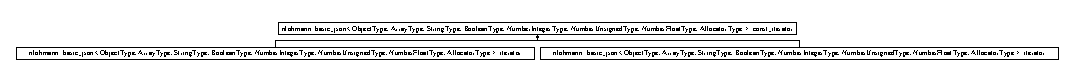
\includegraphics[height=0.568528cm]{d0/d12/classnlohmann_1_1basic__json_1_1const__iterator}
\end{center}
\end{figure}
\subsection*{Public Types}
\begin{DoxyCompactItemize}
\item 
\hypertarget{classnlohmann_1_1basic__json_1_1const__iterator_a9ea0497199b1e96ce9cadd1f202ec343_a9ea0497199b1e96ce9cadd1f202ec343}{using \hyperlink{classnlohmann_1_1basic__json_1_1const__iterator_a9ea0497199b1e96ce9cadd1f202ec343_a9ea0497199b1e96ce9cadd1f202ec343}{value\-\_\-type} = typename \hyperlink{classnlohmann_1_1basic__json_ac8d45b57874b4a6e9c07f7d3b5daa1f9_ac8d45b57874b4a6e9c07f7d3b5daa1f9}{basic\-\_\-json\-::value\-\_\-type}}\label{classnlohmann_1_1basic__json_1_1const__iterator_a9ea0497199b1e96ce9cadd1f202ec343_a9ea0497199b1e96ce9cadd1f202ec343}

\begin{DoxyCompactList}\small\item\em the type of the values when the iterator is dereferenced \end{DoxyCompactList}\item 
\hypertarget{classnlohmann_1_1basic__json_1_1const__iterator_a49d7c3e9ef3280df03052cce988b792f_a49d7c3e9ef3280df03052cce988b792f}{using \hyperlink{classnlohmann_1_1basic__json_1_1const__iterator_a49d7c3e9ef3280df03052cce988b792f_a49d7c3e9ef3280df03052cce988b792f}{difference\-\_\-type} = typename \hyperlink{classnlohmann_1_1basic__json_aec316934a555dd1acdd3600e5d4a4cdf_aec316934a555dd1acdd3600e5d4a4cdf}{basic\-\_\-json\-::difference\-\_\-type}}\label{classnlohmann_1_1basic__json_1_1const__iterator_a49d7c3e9ef3280df03052cce988b792f_a49d7c3e9ef3280df03052cce988b792f}

\begin{DoxyCompactList}\small\item\em a type to represent differences between iterators \end{DoxyCompactList}\item 
\hypertarget{classnlohmann_1_1basic__json_1_1const__iterator_a1da96fc3054d547e7706d3a2f073f389_a1da96fc3054d547e7706d3a2f073f389}{using \hyperlink{classnlohmann_1_1basic__json_1_1const__iterator_a1da96fc3054d547e7706d3a2f073f389_a1da96fc3054d547e7706d3a2f073f389}{pointer} = typename \hyperlink{classnlohmann_1_1basic__json_a06efb200b69942eacd1ea22d0f6ccebb_a06efb200b69942eacd1ea22d0f6ccebb}{basic\-\_\-json\-::const\-\_\-pointer}}\label{classnlohmann_1_1basic__json_1_1const__iterator_a1da96fc3054d547e7706d3a2f073f389_a1da96fc3054d547e7706d3a2f073f389}

\begin{DoxyCompactList}\small\item\em defines a pointer to the type iterated over (value\-\_\-type) \end{DoxyCompactList}\item 
\hypertarget{classnlohmann_1_1basic__json_1_1const__iterator_aefd248cac6493eed1e6ff53ba6a63eb2_aefd248cac6493eed1e6ff53ba6a63eb2}{using \hyperlink{classnlohmann_1_1basic__json_1_1const__iterator_aefd248cac6493eed1e6ff53ba6a63eb2_aefd248cac6493eed1e6ff53ba6a63eb2}{reference} = typename \hyperlink{classnlohmann_1_1basic__json_af677a29b0e66edc9f66e5167e4667071_af677a29b0e66edc9f66e5167e4667071}{basic\-\_\-json\-::const\-\_\-reference}}\label{classnlohmann_1_1basic__json_1_1const__iterator_aefd248cac6493eed1e6ff53ba6a63eb2_aefd248cac6493eed1e6ff53ba6a63eb2}

\begin{DoxyCompactList}\small\item\em defines a reference to the type iterated over (value\-\_\-type) \end{DoxyCompactList}\item 
\hypertarget{classnlohmann_1_1basic__json_1_1const__iterator_a821560d64f50525162097f19b1392e7f_a821560d64f50525162097f19b1392e7f}{using \hyperlink{classnlohmann_1_1basic__json_1_1const__iterator_a821560d64f50525162097f19b1392e7f_a821560d64f50525162097f19b1392e7f}{iterator\-\_\-category} = std\-::bidirectional\-\_\-iterator\-\_\-tag}\label{classnlohmann_1_1basic__json_1_1const__iterator_a821560d64f50525162097f19b1392e7f_a821560d64f50525162097f19b1392e7f}

\begin{DoxyCompactList}\small\item\em the category of the iterator \end{DoxyCompactList}\item 
\hypertarget{classnlohmann_1_1basic__json_1_1const__iterator_a9ea0497199b1e96ce9cadd1f202ec343_a9ea0497199b1e96ce9cadd1f202ec343}{using \hyperlink{classnlohmann_1_1basic__json_1_1const__iterator_a9ea0497199b1e96ce9cadd1f202ec343_a9ea0497199b1e96ce9cadd1f202ec343}{value\-\_\-type} = typename \hyperlink{classnlohmann_1_1basic__json_ac8d45b57874b4a6e9c07f7d3b5daa1f9_ac8d45b57874b4a6e9c07f7d3b5daa1f9}{basic\-\_\-json\-::value\-\_\-type}}\label{classnlohmann_1_1basic__json_1_1const__iterator_a9ea0497199b1e96ce9cadd1f202ec343_a9ea0497199b1e96ce9cadd1f202ec343}

\begin{DoxyCompactList}\small\item\em the type of the values when the iterator is dereferenced \end{DoxyCompactList}\item 
\hypertarget{classnlohmann_1_1basic__json_1_1const__iterator_a49d7c3e9ef3280df03052cce988b792f_a49d7c3e9ef3280df03052cce988b792f}{using \hyperlink{classnlohmann_1_1basic__json_1_1const__iterator_a49d7c3e9ef3280df03052cce988b792f_a49d7c3e9ef3280df03052cce988b792f}{difference\-\_\-type} = typename \hyperlink{classnlohmann_1_1basic__json_aec316934a555dd1acdd3600e5d4a4cdf_aec316934a555dd1acdd3600e5d4a4cdf}{basic\-\_\-json\-::difference\-\_\-type}}\label{classnlohmann_1_1basic__json_1_1const__iterator_a49d7c3e9ef3280df03052cce988b792f_a49d7c3e9ef3280df03052cce988b792f}

\begin{DoxyCompactList}\small\item\em a type to represent differences between iterators \end{DoxyCompactList}\item 
\hypertarget{classnlohmann_1_1basic__json_1_1const__iterator_a1da96fc3054d547e7706d3a2f073f389_a1da96fc3054d547e7706d3a2f073f389}{using \hyperlink{classnlohmann_1_1basic__json_1_1const__iterator_a1da96fc3054d547e7706d3a2f073f389_a1da96fc3054d547e7706d3a2f073f389}{pointer} = typename \hyperlink{classnlohmann_1_1basic__json_a06efb200b69942eacd1ea22d0f6ccebb_a06efb200b69942eacd1ea22d0f6ccebb}{basic\-\_\-json\-::const\-\_\-pointer}}\label{classnlohmann_1_1basic__json_1_1const__iterator_a1da96fc3054d547e7706d3a2f073f389_a1da96fc3054d547e7706d3a2f073f389}

\begin{DoxyCompactList}\small\item\em defines a pointer to the type iterated over (value\-\_\-type) \end{DoxyCompactList}\item 
\hypertarget{classnlohmann_1_1basic__json_1_1const__iterator_aefd248cac6493eed1e6ff53ba6a63eb2_aefd248cac6493eed1e6ff53ba6a63eb2}{using \hyperlink{classnlohmann_1_1basic__json_1_1const__iterator_aefd248cac6493eed1e6ff53ba6a63eb2_aefd248cac6493eed1e6ff53ba6a63eb2}{reference} = typename \hyperlink{classnlohmann_1_1basic__json_af677a29b0e66edc9f66e5167e4667071_af677a29b0e66edc9f66e5167e4667071}{basic\-\_\-json\-::const\-\_\-reference}}\label{classnlohmann_1_1basic__json_1_1const__iterator_aefd248cac6493eed1e6ff53ba6a63eb2_aefd248cac6493eed1e6ff53ba6a63eb2}

\begin{DoxyCompactList}\small\item\em defines a reference to the type iterated over (value\-\_\-type) \end{DoxyCompactList}\item 
\hypertarget{classnlohmann_1_1basic__json_1_1const__iterator_a821560d64f50525162097f19b1392e7f_a821560d64f50525162097f19b1392e7f}{using \hyperlink{classnlohmann_1_1basic__json_1_1const__iterator_a821560d64f50525162097f19b1392e7f_a821560d64f50525162097f19b1392e7f}{iterator\-\_\-category} = std\-::bidirectional\-\_\-iterator\-\_\-tag}\label{classnlohmann_1_1basic__json_1_1const__iterator_a821560d64f50525162097f19b1392e7f_a821560d64f50525162097f19b1392e7f}

\begin{DoxyCompactList}\small\item\em the category of the iterator \end{DoxyCompactList}\end{DoxyCompactItemize}
\subsection*{Public Member Functions}
\begin{DoxyCompactItemize}
\item 
\hypertarget{classnlohmann_1_1basic__json_1_1const__iterator_ac6fdaff67857f82a623e5cc253917639_ac6fdaff67857f82a623e5cc253917639}{\hyperlink{classnlohmann_1_1basic__json_1_1const__iterator_ac6fdaff67857f82a623e5cc253917639_ac6fdaff67857f82a623e5cc253917639}{const\-\_\-iterator} ()=default}\label{classnlohmann_1_1basic__json_1_1const__iterator_ac6fdaff67857f82a623e5cc253917639_ac6fdaff67857f82a623e5cc253917639}

\begin{DoxyCompactList}\small\item\em default constructor \end{DoxyCompactList}\item 
\hypertarget{classnlohmann_1_1basic__json_1_1const__iterator_a23de834b11bd895209aa65c100ab9ceb_a23de834b11bd895209aa65c100ab9ceb}{\hyperlink{classnlohmann_1_1basic__json_1_1const__iterator_a23de834b11bd895209aa65c100ab9ceb_a23de834b11bd895209aa65c100ab9ceb}{const\-\_\-iterator} (\hyperlink{classnlohmann_1_1basic__json_1_1const__iterator_a1da96fc3054d547e7706d3a2f073f389_a1da96fc3054d547e7706d3a2f073f389}{pointer} \hyperlink{classnlohmann_1_1basic__json_ad25b2f8c21e241e2d63455537a9294ff_ad25b2f8c21e241e2d63455537a9294ff}{object}) noexcept}\label{classnlohmann_1_1basic__json_1_1const__iterator_a23de834b11bd895209aa65c100ab9ceb_a23de834b11bd895209aa65c100ab9ceb}

\begin{DoxyCompactList}\small\item\em constructor for a given J\-S\-O\-N instance \end{DoxyCompactList}\item 
\hypertarget{classnlohmann_1_1basic__json_1_1const__iterator_a6b950c6bc081ac1ec1540ec05ceb2603_a6b950c6bc081ac1ec1540ec05ceb2603}{\hyperlink{classnlohmann_1_1basic__json_1_1const__iterator_a6b950c6bc081ac1ec1540ec05ceb2603_a6b950c6bc081ac1ec1540ec05ceb2603}{const\-\_\-iterator} (const \hyperlink{classnlohmann_1_1basic__json_1_1iterator}{iterator} \&other) noexcept}\label{classnlohmann_1_1basic__json_1_1const__iterator_a6b950c6bc081ac1ec1540ec05ceb2603_a6b950c6bc081ac1ec1540ec05ceb2603}

\begin{DoxyCompactList}\small\item\em copy constructor given a nonconst iterator \end{DoxyCompactList}\item 
\hypertarget{classnlohmann_1_1basic__json_1_1const__iterator_a18c35a6735d3da96b4fc026421c05dd8_a18c35a6735d3da96b4fc026421c05dd8}{\hyperlink{classnlohmann_1_1basic__json_1_1const__iterator_a18c35a6735d3da96b4fc026421c05dd8_a18c35a6735d3da96b4fc026421c05dd8}{const\-\_\-iterator} (const \hyperlink{classnlohmann_1_1basic__json_1_1const__iterator}{const\-\_\-iterator} \&other) noexcept}\label{classnlohmann_1_1basic__json_1_1const__iterator_a18c35a6735d3da96b4fc026421c05dd8_a18c35a6735d3da96b4fc026421c05dd8}

\begin{DoxyCompactList}\small\item\em copy constructor \end{DoxyCompactList}\item 
\hypertarget{classnlohmann_1_1basic__json_1_1const__iterator_adb91f1fc32926a0ac7a5eeaa47175642_adb91f1fc32926a0ac7a5eeaa47175642}{\hyperlink{classnlohmann_1_1basic__json_1_1const__iterator}{const\-\_\-iterator} \& \hyperlink{classnlohmann_1_1basic__json_1_1const__iterator_adb91f1fc32926a0ac7a5eeaa47175642_adb91f1fc32926a0ac7a5eeaa47175642}{operator=} (\hyperlink{classnlohmann_1_1basic__json_1_1const__iterator}{const\-\_\-iterator} other) noexcept(std\-::is\-\_\-nothrow\-\_\-move\-\_\-constructible$<$ \hyperlink{classnlohmann_1_1basic__json_1_1const__iterator_a1da96fc3054d547e7706d3a2f073f389_a1da96fc3054d547e7706d3a2f073f389}{pointer} $>$\-::\hyperlink{classnlohmann_1_1basic__json_1_1const__iterator_ac75e80d30b6169ee2a29ec93fb4d2acd_ac75e80d30b6169ee2a29ec93fb4d2acd}{value} andstd\-::is\-\_\-nothrow\-\_\-move\-\_\-assignable$<$ \hyperlink{classnlohmann_1_1basic__json_1_1const__iterator_a1da96fc3054d547e7706d3a2f073f389_a1da96fc3054d547e7706d3a2f073f389}{pointer} $>$\-::\hyperlink{classnlohmann_1_1basic__json_1_1const__iterator_ac75e80d30b6169ee2a29ec93fb4d2acd_ac75e80d30b6169ee2a29ec93fb4d2acd}{value} andstd\-::is\-\_\-nothrow\-\_\-move\-\_\-constructible$<$ \hyperlink{structnlohmann_1_1basic__json_1_1internal__iterator}{internal\-\_\-iterator} $>$\-::\hyperlink{classnlohmann_1_1basic__json_1_1const__iterator_ac75e80d30b6169ee2a29ec93fb4d2acd_ac75e80d30b6169ee2a29ec93fb4d2acd}{value} andstd\-::is\-\_\-nothrow\-\_\-move\-\_\-assignable$<$ \hyperlink{structnlohmann_1_1basic__json_1_1internal__iterator}{internal\-\_\-iterator} $>$\-::\hyperlink{classnlohmann_1_1basic__json_1_1const__iterator_ac75e80d30b6169ee2a29ec93fb4d2acd_ac75e80d30b6169ee2a29ec93fb4d2acd}{value})}\label{classnlohmann_1_1basic__json_1_1const__iterator_adb91f1fc32926a0ac7a5eeaa47175642_adb91f1fc32926a0ac7a5eeaa47175642}

\begin{DoxyCompactList}\small\item\em copy assignment \end{DoxyCompactList}\item 
\hypertarget{classnlohmann_1_1basic__json_1_1const__iterator_ab3029a1a83cf46dc28ad443bbad0c74d_ab3029a1a83cf46dc28ad443bbad0c74d}{\hyperlink{classnlohmann_1_1basic__json_1_1const__iterator_aefd248cac6493eed1e6ff53ba6a63eb2_aefd248cac6493eed1e6ff53ba6a63eb2}{reference} \hyperlink{classnlohmann_1_1basic__json_1_1const__iterator_ab3029a1a83cf46dc28ad443bbad0c74d_ab3029a1a83cf46dc28ad443bbad0c74d}{operator$\ast$} () const }\label{classnlohmann_1_1basic__json_1_1const__iterator_ab3029a1a83cf46dc28ad443bbad0c74d_ab3029a1a83cf46dc28ad443bbad0c74d}

\begin{DoxyCompactList}\small\item\em return a reference to the value pointed to by the iterator \end{DoxyCompactList}\item 
\hypertarget{classnlohmann_1_1basic__json_1_1const__iterator_a8be837e4d902887676dd837abe9098d3_a8be837e4d902887676dd837abe9098d3}{\hyperlink{classnlohmann_1_1basic__json_1_1const__iterator_a1da96fc3054d547e7706d3a2f073f389_a1da96fc3054d547e7706d3a2f073f389}{pointer} \hyperlink{classnlohmann_1_1basic__json_1_1const__iterator_a8be837e4d902887676dd837abe9098d3_a8be837e4d902887676dd837abe9098d3}{operator-\/$>$} () const }\label{classnlohmann_1_1basic__json_1_1const__iterator_a8be837e4d902887676dd837abe9098d3_a8be837e4d902887676dd837abe9098d3}

\begin{DoxyCompactList}\small\item\em dereference the iterator \end{DoxyCompactList}\item 
\hypertarget{classnlohmann_1_1basic__json_1_1const__iterator_a8dbaec5bf8ccba3225520356629061cb_a8dbaec5bf8ccba3225520356629061cb}{\hyperlink{classnlohmann_1_1basic__json_1_1const__iterator}{const\-\_\-iterator} \hyperlink{classnlohmann_1_1basic__json_1_1const__iterator_a8dbaec5bf8ccba3225520356629061cb_a8dbaec5bf8ccba3225520356629061cb}{operator++} (int)}\label{classnlohmann_1_1basic__json_1_1const__iterator_a8dbaec5bf8ccba3225520356629061cb_a8dbaec5bf8ccba3225520356629061cb}

\begin{DoxyCompactList}\small\item\em post-\/increment (it++) \end{DoxyCompactList}\item 
\hypertarget{classnlohmann_1_1basic__json_1_1const__iterator_a8fbb15efd97599209a7def77af8e748e_a8fbb15efd97599209a7def77af8e748e}{\hyperlink{classnlohmann_1_1basic__json_1_1const__iterator}{const\-\_\-iterator} \& \hyperlink{classnlohmann_1_1basic__json_1_1const__iterator_a8fbb15efd97599209a7def77af8e748e_a8fbb15efd97599209a7def77af8e748e}{operator++} ()}\label{classnlohmann_1_1basic__json_1_1const__iterator_a8fbb15efd97599209a7def77af8e748e_a8fbb15efd97599209a7def77af8e748e}

\begin{DoxyCompactList}\small\item\em pre-\/increment (++it) \end{DoxyCompactList}\item 
\hypertarget{classnlohmann_1_1basic__json_1_1const__iterator_a6cab1c2ed7e2a014980e2a5717f43a64_a6cab1c2ed7e2a014980e2a5717f43a64}{\hyperlink{classnlohmann_1_1basic__json_1_1const__iterator}{const\-\_\-iterator} \hyperlink{classnlohmann_1_1basic__json_1_1const__iterator_a6cab1c2ed7e2a014980e2a5717f43a64_a6cab1c2ed7e2a014980e2a5717f43a64}{operator-\/-\/} (int)}\label{classnlohmann_1_1basic__json_1_1const__iterator_a6cab1c2ed7e2a014980e2a5717f43a64_a6cab1c2ed7e2a014980e2a5717f43a64}

\begin{DoxyCompactList}\small\item\em post-\/decrement (it--) \end{DoxyCompactList}\item 
\hypertarget{classnlohmann_1_1basic__json_1_1const__iterator_adeb2ff3fdf3cc301b72db109934c9199_adeb2ff3fdf3cc301b72db109934c9199}{\hyperlink{classnlohmann_1_1basic__json_1_1const__iterator}{const\-\_\-iterator} \& \hyperlink{classnlohmann_1_1basic__json_1_1const__iterator_adeb2ff3fdf3cc301b72db109934c9199_adeb2ff3fdf3cc301b72db109934c9199}{operator-\/-\/} ()}\label{classnlohmann_1_1basic__json_1_1const__iterator_adeb2ff3fdf3cc301b72db109934c9199_adeb2ff3fdf3cc301b72db109934c9199}

\begin{DoxyCompactList}\small\item\em pre-\/decrement (--it) \end{DoxyCompactList}\item 
\hypertarget{classnlohmann_1_1basic__json_1_1const__iterator_ab4c0b9baaec9ebc4837158e272f6c803_ab4c0b9baaec9ebc4837158e272f6c803}{bool \hyperlink{classnlohmann_1_1basic__json_1_1const__iterator_ab4c0b9baaec9ebc4837158e272f6c803_ab4c0b9baaec9ebc4837158e272f6c803}{operator==} (const \hyperlink{classnlohmann_1_1basic__json_1_1const__iterator}{const\-\_\-iterator} \&other) const }\label{classnlohmann_1_1basic__json_1_1const__iterator_ab4c0b9baaec9ebc4837158e272f6c803_ab4c0b9baaec9ebc4837158e272f6c803}

\begin{DoxyCompactList}\small\item\em comparison\-: equal \end{DoxyCompactList}\item 
\hypertarget{classnlohmann_1_1basic__json_1_1const__iterator_a9e4c6e48e3c2f3ff357ef8215b8c8fca_a9e4c6e48e3c2f3ff357ef8215b8c8fca}{bool \hyperlink{classnlohmann_1_1basic__json_1_1const__iterator_a9e4c6e48e3c2f3ff357ef8215b8c8fca_a9e4c6e48e3c2f3ff357ef8215b8c8fca}{operator!=} (const \hyperlink{classnlohmann_1_1basic__json_1_1const__iterator}{const\-\_\-iterator} \&other) const }\label{classnlohmann_1_1basic__json_1_1const__iterator_a9e4c6e48e3c2f3ff357ef8215b8c8fca_a9e4c6e48e3c2f3ff357ef8215b8c8fca}

\begin{DoxyCompactList}\small\item\em comparison\-: not equal \end{DoxyCompactList}\item 
\hypertarget{classnlohmann_1_1basic__json_1_1const__iterator_a65f491b515e5967e9c0b40289e3c0ff3_a65f491b515e5967e9c0b40289e3c0ff3}{bool \hyperlink{classnlohmann_1_1basic__json_1_1const__iterator_a65f491b515e5967e9c0b40289e3c0ff3_a65f491b515e5967e9c0b40289e3c0ff3}{operator$<$} (const \hyperlink{classnlohmann_1_1basic__json_1_1const__iterator}{const\-\_\-iterator} \&other) const }\label{classnlohmann_1_1basic__json_1_1const__iterator_a65f491b515e5967e9c0b40289e3c0ff3_a65f491b515e5967e9c0b40289e3c0ff3}

\begin{DoxyCompactList}\small\item\em comparison\-: smaller \end{DoxyCompactList}\item 
\hypertarget{classnlohmann_1_1basic__json_1_1const__iterator_a6b682f09787eff62f03493d45aa05902_a6b682f09787eff62f03493d45aa05902}{bool \hyperlink{classnlohmann_1_1basic__json_1_1const__iterator_a6b682f09787eff62f03493d45aa05902_a6b682f09787eff62f03493d45aa05902}{operator$<$=} (const \hyperlink{classnlohmann_1_1basic__json_1_1const__iterator}{const\-\_\-iterator} \&other) const }\label{classnlohmann_1_1basic__json_1_1const__iterator_a6b682f09787eff62f03493d45aa05902_a6b682f09787eff62f03493d45aa05902}

\begin{DoxyCompactList}\small\item\em comparison\-: less than or equal \end{DoxyCompactList}\item 
\hypertarget{classnlohmann_1_1basic__json_1_1const__iterator_acb6cd0ff760933afeb7f93e5207f3646_acb6cd0ff760933afeb7f93e5207f3646}{bool \hyperlink{classnlohmann_1_1basic__json_1_1const__iterator_acb6cd0ff760933afeb7f93e5207f3646_acb6cd0ff760933afeb7f93e5207f3646}{operator$>$} (const \hyperlink{classnlohmann_1_1basic__json_1_1const__iterator}{const\-\_\-iterator} \&other) const }\label{classnlohmann_1_1basic__json_1_1const__iterator_acb6cd0ff760933afeb7f93e5207f3646_acb6cd0ff760933afeb7f93e5207f3646}

\begin{DoxyCompactList}\small\item\em comparison\-: greater than \end{DoxyCompactList}\item 
\hypertarget{classnlohmann_1_1basic__json_1_1const__iterator_af6941c3711dabb2e64960dd57e00d201_af6941c3711dabb2e64960dd57e00d201}{bool \hyperlink{classnlohmann_1_1basic__json_1_1const__iterator_af6941c3711dabb2e64960dd57e00d201_af6941c3711dabb2e64960dd57e00d201}{operator$>$=} (const \hyperlink{classnlohmann_1_1basic__json_1_1const__iterator}{const\-\_\-iterator} \&other) const }\label{classnlohmann_1_1basic__json_1_1const__iterator_af6941c3711dabb2e64960dd57e00d201_af6941c3711dabb2e64960dd57e00d201}

\begin{DoxyCompactList}\small\item\em comparison\-: greater than or equal \end{DoxyCompactList}\item 
\hypertarget{classnlohmann_1_1basic__json_1_1const__iterator_a0d5820d1dda9dea3bbeb029cacf68522_a0d5820d1dda9dea3bbeb029cacf68522}{\hyperlink{classnlohmann_1_1basic__json_1_1const__iterator}{const\-\_\-iterator} \& \hyperlink{classnlohmann_1_1basic__json_1_1const__iterator_a0d5820d1dda9dea3bbeb029cacf68522_a0d5820d1dda9dea3bbeb029cacf68522}{operator+=} (\hyperlink{classnlohmann_1_1basic__json_1_1const__iterator_a49d7c3e9ef3280df03052cce988b792f_a49d7c3e9ef3280df03052cce988b792f}{difference\-\_\-type} i)}\label{classnlohmann_1_1basic__json_1_1const__iterator_a0d5820d1dda9dea3bbeb029cacf68522_a0d5820d1dda9dea3bbeb029cacf68522}

\begin{DoxyCompactList}\small\item\em add to iterator \end{DoxyCompactList}\item 
\hypertarget{classnlohmann_1_1basic__json_1_1const__iterator_aefac8f3e390ac917f021761f4a8f8e71_aefac8f3e390ac917f021761f4a8f8e71}{\hyperlink{classnlohmann_1_1basic__json_1_1const__iterator}{const\-\_\-iterator} \& \hyperlink{classnlohmann_1_1basic__json_1_1const__iterator_aefac8f3e390ac917f021761f4a8f8e71_aefac8f3e390ac917f021761f4a8f8e71}{operator-\/=} (\hyperlink{classnlohmann_1_1basic__json_1_1const__iterator_a49d7c3e9ef3280df03052cce988b792f_a49d7c3e9ef3280df03052cce988b792f}{difference\-\_\-type} i)}\label{classnlohmann_1_1basic__json_1_1const__iterator_aefac8f3e390ac917f021761f4a8f8e71_aefac8f3e390ac917f021761f4a8f8e71}

\begin{DoxyCompactList}\small\item\em subtract from iterator \end{DoxyCompactList}\item 
\hypertarget{classnlohmann_1_1basic__json_1_1const__iterator_a7a80257f2303210b0a5d056fc0b30b40_a7a80257f2303210b0a5d056fc0b30b40}{\hyperlink{classnlohmann_1_1basic__json_1_1const__iterator}{const\-\_\-iterator} \hyperlink{classnlohmann_1_1basic__json_1_1const__iterator_a7a80257f2303210b0a5d056fc0b30b40_a7a80257f2303210b0a5d056fc0b30b40}{operator+} (\hyperlink{classnlohmann_1_1basic__json_1_1const__iterator_a49d7c3e9ef3280df03052cce988b792f_a49d7c3e9ef3280df03052cce988b792f}{difference\-\_\-type} i)}\label{classnlohmann_1_1basic__json_1_1const__iterator_a7a80257f2303210b0a5d056fc0b30b40_a7a80257f2303210b0a5d056fc0b30b40}

\begin{DoxyCompactList}\small\item\em add to iterator \end{DoxyCompactList}\item 
\hypertarget{classnlohmann_1_1basic__json_1_1const__iterator_abc4552ba2fe39e7901a83dd6d4dec151_abc4552ba2fe39e7901a83dd6d4dec151}{\hyperlink{classnlohmann_1_1basic__json_1_1const__iterator}{const\-\_\-iterator} \hyperlink{classnlohmann_1_1basic__json_1_1const__iterator_abc4552ba2fe39e7901a83dd6d4dec151_abc4552ba2fe39e7901a83dd6d4dec151}{operator-\/} (\hyperlink{classnlohmann_1_1basic__json_1_1const__iterator_a49d7c3e9ef3280df03052cce988b792f_a49d7c3e9ef3280df03052cce988b792f}{difference\-\_\-type} i)}\label{classnlohmann_1_1basic__json_1_1const__iterator_abc4552ba2fe39e7901a83dd6d4dec151_abc4552ba2fe39e7901a83dd6d4dec151}

\begin{DoxyCompactList}\small\item\em subtract from iterator \end{DoxyCompactList}\item 
\hypertarget{classnlohmann_1_1basic__json_1_1const__iterator_a5e4d98a8f95e2eccde8cd48c19efa196_a5e4d98a8f95e2eccde8cd48c19efa196}{\hyperlink{classnlohmann_1_1basic__json_1_1const__iterator_a49d7c3e9ef3280df03052cce988b792f_a49d7c3e9ef3280df03052cce988b792f}{difference\-\_\-type} \hyperlink{classnlohmann_1_1basic__json_1_1const__iterator_a5e4d98a8f95e2eccde8cd48c19efa196_a5e4d98a8f95e2eccde8cd48c19efa196}{operator-\/} (const \hyperlink{classnlohmann_1_1basic__json_1_1const__iterator}{const\-\_\-iterator} \&other) const }\label{classnlohmann_1_1basic__json_1_1const__iterator_a5e4d98a8f95e2eccde8cd48c19efa196_a5e4d98a8f95e2eccde8cd48c19efa196}

\begin{DoxyCompactList}\small\item\em return difference \end{DoxyCompactList}\item 
\hypertarget{classnlohmann_1_1basic__json_1_1const__iterator_a7bd530bfbbc58ac77308c087120c21fa_a7bd530bfbbc58ac77308c087120c21fa}{\hyperlink{classnlohmann_1_1basic__json_1_1const__iterator_aefd248cac6493eed1e6ff53ba6a63eb2_aefd248cac6493eed1e6ff53ba6a63eb2}{reference} \hyperlink{classnlohmann_1_1basic__json_1_1const__iterator_a7bd530bfbbc58ac77308c087120c21fa_a7bd530bfbbc58ac77308c087120c21fa}{operator\mbox{[}$\,$\mbox{]}} (\hyperlink{classnlohmann_1_1basic__json_1_1const__iterator_a49d7c3e9ef3280df03052cce988b792f_a49d7c3e9ef3280df03052cce988b792f}{difference\-\_\-type} n) const }\label{classnlohmann_1_1basic__json_1_1const__iterator_a7bd530bfbbc58ac77308c087120c21fa_a7bd530bfbbc58ac77308c087120c21fa}

\begin{DoxyCompactList}\small\item\em access to successor \end{DoxyCompactList}\item 
\hypertarget{classnlohmann_1_1basic__json_1_1const__iterator_a5d4320e24fcb7df041ff2c95d976dba0_a5d4320e24fcb7df041ff2c95d976dba0}{object\-\_\-t\-::key\-\_\-type \hyperlink{classnlohmann_1_1basic__json_1_1const__iterator_a5d4320e24fcb7df041ff2c95d976dba0_a5d4320e24fcb7df041ff2c95d976dba0}{key} () const }\label{classnlohmann_1_1basic__json_1_1const__iterator_a5d4320e24fcb7df041ff2c95d976dba0_a5d4320e24fcb7df041ff2c95d976dba0}

\begin{DoxyCompactList}\small\item\em return the key of an object iterator \end{DoxyCompactList}\item 
\hypertarget{classnlohmann_1_1basic__json_1_1const__iterator_ac75e80d30b6169ee2a29ec93fb4d2acd_ac75e80d30b6169ee2a29ec93fb4d2acd}{\hyperlink{classnlohmann_1_1basic__json_1_1const__iterator_aefd248cac6493eed1e6ff53ba6a63eb2_aefd248cac6493eed1e6ff53ba6a63eb2}{reference} \hyperlink{classnlohmann_1_1basic__json_1_1const__iterator_ac75e80d30b6169ee2a29ec93fb4d2acd_ac75e80d30b6169ee2a29ec93fb4d2acd}{value} () const }\label{classnlohmann_1_1basic__json_1_1const__iterator_ac75e80d30b6169ee2a29ec93fb4d2acd_ac75e80d30b6169ee2a29ec93fb4d2acd}

\begin{DoxyCompactList}\small\item\em return the value of an iterator \end{DoxyCompactList}\item 
\hypertarget{classnlohmann_1_1basic__json_1_1const__iterator_ac6fdaff67857f82a623e5cc253917639_ac6fdaff67857f82a623e5cc253917639}{\hyperlink{classnlohmann_1_1basic__json_1_1const__iterator_ac6fdaff67857f82a623e5cc253917639_ac6fdaff67857f82a623e5cc253917639}{const\-\_\-iterator} ()=default}\label{classnlohmann_1_1basic__json_1_1const__iterator_ac6fdaff67857f82a623e5cc253917639_ac6fdaff67857f82a623e5cc253917639}

\begin{DoxyCompactList}\small\item\em default constructor \end{DoxyCompactList}\item 
\hypertarget{classnlohmann_1_1basic__json_1_1const__iterator_a23de834b11bd895209aa65c100ab9ceb_a23de834b11bd895209aa65c100ab9ceb}{\hyperlink{classnlohmann_1_1basic__json_1_1const__iterator_a23de834b11bd895209aa65c100ab9ceb_a23de834b11bd895209aa65c100ab9ceb}{const\-\_\-iterator} (\hyperlink{classnlohmann_1_1basic__json_1_1const__iterator_a1da96fc3054d547e7706d3a2f073f389_a1da96fc3054d547e7706d3a2f073f389}{pointer} \hyperlink{classnlohmann_1_1basic__json_ad25b2f8c21e241e2d63455537a9294ff_ad25b2f8c21e241e2d63455537a9294ff}{object}) noexcept}\label{classnlohmann_1_1basic__json_1_1const__iterator_a23de834b11bd895209aa65c100ab9ceb_a23de834b11bd895209aa65c100ab9ceb}

\begin{DoxyCompactList}\small\item\em constructor for a given J\-S\-O\-N instance \end{DoxyCompactList}\item 
\hypertarget{classnlohmann_1_1basic__json_1_1const__iterator_a6b950c6bc081ac1ec1540ec05ceb2603_a6b950c6bc081ac1ec1540ec05ceb2603}{\hyperlink{classnlohmann_1_1basic__json_1_1const__iterator_a6b950c6bc081ac1ec1540ec05ceb2603_a6b950c6bc081ac1ec1540ec05ceb2603}{const\-\_\-iterator} (const \hyperlink{classnlohmann_1_1basic__json_1_1iterator}{iterator} \&other) noexcept}\label{classnlohmann_1_1basic__json_1_1const__iterator_a6b950c6bc081ac1ec1540ec05ceb2603_a6b950c6bc081ac1ec1540ec05ceb2603}

\begin{DoxyCompactList}\small\item\em copy constructor given a nonconst iterator \end{DoxyCompactList}\item 
\hypertarget{classnlohmann_1_1basic__json_1_1const__iterator_a18c35a6735d3da96b4fc026421c05dd8_a18c35a6735d3da96b4fc026421c05dd8}{\hyperlink{classnlohmann_1_1basic__json_1_1const__iterator_a18c35a6735d3da96b4fc026421c05dd8_a18c35a6735d3da96b4fc026421c05dd8}{const\-\_\-iterator} (const \hyperlink{classnlohmann_1_1basic__json_1_1const__iterator}{const\-\_\-iterator} \&other) noexcept}\label{classnlohmann_1_1basic__json_1_1const__iterator_a18c35a6735d3da96b4fc026421c05dd8_a18c35a6735d3da96b4fc026421c05dd8}

\begin{DoxyCompactList}\small\item\em copy constructor \end{DoxyCompactList}\item 
\hypertarget{classnlohmann_1_1basic__json_1_1const__iterator_adb91f1fc32926a0ac7a5eeaa47175642_adb91f1fc32926a0ac7a5eeaa47175642}{\hyperlink{classnlohmann_1_1basic__json_1_1const__iterator}{const\-\_\-iterator} \& \hyperlink{classnlohmann_1_1basic__json_1_1const__iterator_adb91f1fc32926a0ac7a5eeaa47175642_adb91f1fc32926a0ac7a5eeaa47175642}{operator=} (\hyperlink{classnlohmann_1_1basic__json_1_1const__iterator}{const\-\_\-iterator} other) noexcept(std\-::is\-\_\-nothrow\-\_\-move\-\_\-constructible$<$ \hyperlink{classnlohmann_1_1basic__json_1_1const__iterator_a1da96fc3054d547e7706d3a2f073f389_a1da96fc3054d547e7706d3a2f073f389}{pointer} $>$\-::\hyperlink{classnlohmann_1_1basic__json_1_1const__iterator_ac75e80d30b6169ee2a29ec93fb4d2acd_ac75e80d30b6169ee2a29ec93fb4d2acd}{value} andstd\-::is\-\_\-nothrow\-\_\-move\-\_\-assignable$<$ \hyperlink{classnlohmann_1_1basic__json_1_1const__iterator_a1da96fc3054d547e7706d3a2f073f389_a1da96fc3054d547e7706d3a2f073f389}{pointer} $>$\-::\hyperlink{classnlohmann_1_1basic__json_1_1const__iterator_ac75e80d30b6169ee2a29ec93fb4d2acd_ac75e80d30b6169ee2a29ec93fb4d2acd}{value} andstd\-::is\-\_\-nothrow\-\_\-move\-\_\-constructible$<$ \hyperlink{structnlohmann_1_1basic__json_1_1internal__iterator}{internal\-\_\-iterator} $>$\-::\hyperlink{classnlohmann_1_1basic__json_1_1const__iterator_ac75e80d30b6169ee2a29ec93fb4d2acd_ac75e80d30b6169ee2a29ec93fb4d2acd}{value} andstd\-::is\-\_\-nothrow\-\_\-move\-\_\-assignable$<$ \hyperlink{structnlohmann_1_1basic__json_1_1internal__iterator}{internal\-\_\-iterator} $>$\-::\hyperlink{classnlohmann_1_1basic__json_1_1const__iterator_ac75e80d30b6169ee2a29ec93fb4d2acd_ac75e80d30b6169ee2a29ec93fb4d2acd}{value})}\label{classnlohmann_1_1basic__json_1_1const__iterator_adb91f1fc32926a0ac7a5eeaa47175642_adb91f1fc32926a0ac7a5eeaa47175642}

\begin{DoxyCompactList}\small\item\em copy assignment \end{DoxyCompactList}\item 
\hypertarget{classnlohmann_1_1basic__json_1_1const__iterator_ab3029a1a83cf46dc28ad443bbad0c74d_ab3029a1a83cf46dc28ad443bbad0c74d}{\hyperlink{classnlohmann_1_1basic__json_1_1const__iterator_aefd248cac6493eed1e6ff53ba6a63eb2_aefd248cac6493eed1e6ff53ba6a63eb2}{reference} \hyperlink{classnlohmann_1_1basic__json_1_1const__iterator_ab3029a1a83cf46dc28ad443bbad0c74d_ab3029a1a83cf46dc28ad443bbad0c74d}{operator$\ast$} () const }\label{classnlohmann_1_1basic__json_1_1const__iterator_ab3029a1a83cf46dc28ad443bbad0c74d_ab3029a1a83cf46dc28ad443bbad0c74d}

\begin{DoxyCompactList}\small\item\em return a reference to the value pointed to by the iterator \end{DoxyCompactList}\item 
\hypertarget{classnlohmann_1_1basic__json_1_1const__iterator_a8be837e4d902887676dd837abe9098d3_a8be837e4d902887676dd837abe9098d3}{\hyperlink{classnlohmann_1_1basic__json_1_1const__iterator_a1da96fc3054d547e7706d3a2f073f389_a1da96fc3054d547e7706d3a2f073f389}{pointer} \hyperlink{classnlohmann_1_1basic__json_1_1const__iterator_a8be837e4d902887676dd837abe9098d3_a8be837e4d902887676dd837abe9098d3}{operator-\/$>$} () const }\label{classnlohmann_1_1basic__json_1_1const__iterator_a8be837e4d902887676dd837abe9098d3_a8be837e4d902887676dd837abe9098d3}

\begin{DoxyCompactList}\small\item\em dereference the iterator \end{DoxyCompactList}\item 
\hypertarget{classnlohmann_1_1basic__json_1_1const__iterator_a8dbaec5bf8ccba3225520356629061cb_a8dbaec5bf8ccba3225520356629061cb}{\hyperlink{classnlohmann_1_1basic__json_1_1const__iterator}{const\-\_\-iterator} \hyperlink{classnlohmann_1_1basic__json_1_1const__iterator_a8dbaec5bf8ccba3225520356629061cb_a8dbaec5bf8ccba3225520356629061cb}{operator++} (int)}\label{classnlohmann_1_1basic__json_1_1const__iterator_a8dbaec5bf8ccba3225520356629061cb_a8dbaec5bf8ccba3225520356629061cb}

\begin{DoxyCompactList}\small\item\em post-\/increment (it++) \end{DoxyCompactList}\item 
\hypertarget{classnlohmann_1_1basic__json_1_1const__iterator_a8fbb15efd97599209a7def77af8e748e_a8fbb15efd97599209a7def77af8e748e}{\hyperlink{classnlohmann_1_1basic__json_1_1const__iterator}{const\-\_\-iterator} \& \hyperlink{classnlohmann_1_1basic__json_1_1const__iterator_a8fbb15efd97599209a7def77af8e748e_a8fbb15efd97599209a7def77af8e748e}{operator++} ()}\label{classnlohmann_1_1basic__json_1_1const__iterator_a8fbb15efd97599209a7def77af8e748e_a8fbb15efd97599209a7def77af8e748e}

\begin{DoxyCompactList}\small\item\em pre-\/increment (++it) \end{DoxyCompactList}\item 
\hypertarget{classnlohmann_1_1basic__json_1_1const__iterator_a6cab1c2ed7e2a014980e2a5717f43a64_a6cab1c2ed7e2a014980e2a5717f43a64}{\hyperlink{classnlohmann_1_1basic__json_1_1const__iterator}{const\-\_\-iterator} \hyperlink{classnlohmann_1_1basic__json_1_1const__iterator_a6cab1c2ed7e2a014980e2a5717f43a64_a6cab1c2ed7e2a014980e2a5717f43a64}{operator-\/-\/} (int)}\label{classnlohmann_1_1basic__json_1_1const__iterator_a6cab1c2ed7e2a014980e2a5717f43a64_a6cab1c2ed7e2a014980e2a5717f43a64}

\begin{DoxyCompactList}\small\item\em post-\/decrement (it--) \end{DoxyCompactList}\item 
\hypertarget{classnlohmann_1_1basic__json_1_1const__iterator_adeb2ff3fdf3cc301b72db109934c9199_adeb2ff3fdf3cc301b72db109934c9199}{\hyperlink{classnlohmann_1_1basic__json_1_1const__iterator}{const\-\_\-iterator} \& \hyperlink{classnlohmann_1_1basic__json_1_1const__iterator_adeb2ff3fdf3cc301b72db109934c9199_adeb2ff3fdf3cc301b72db109934c9199}{operator-\/-\/} ()}\label{classnlohmann_1_1basic__json_1_1const__iterator_adeb2ff3fdf3cc301b72db109934c9199_adeb2ff3fdf3cc301b72db109934c9199}

\begin{DoxyCompactList}\small\item\em pre-\/decrement (--it) \end{DoxyCompactList}\item 
\hypertarget{classnlohmann_1_1basic__json_1_1const__iterator_ab4c0b9baaec9ebc4837158e272f6c803_ab4c0b9baaec9ebc4837158e272f6c803}{bool \hyperlink{classnlohmann_1_1basic__json_1_1const__iterator_ab4c0b9baaec9ebc4837158e272f6c803_ab4c0b9baaec9ebc4837158e272f6c803}{operator==} (const \hyperlink{classnlohmann_1_1basic__json_1_1const__iterator}{const\-\_\-iterator} \&other) const }\label{classnlohmann_1_1basic__json_1_1const__iterator_ab4c0b9baaec9ebc4837158e272f6c803_ab4c0b9baaec9ebc4837158e272f6c803}

\begin{DoxyCompactList}\small\item\em comparison\-: equal \end{DoxyCompactList}\item 
\hypertarget{classnlohmann_1_1basic__json_1_1const__iterator_a9e4c6e48e3c2f3ff357ef8215b8c8fca_a9e4c6e48e3c2f3ff357ef8215b8c8fca}{bool \hyperlink{classnlohmann_1_1basic__json_1_1const__iterator_a9e4c6e48e3c2f3ff357ef8215b8c8fca_a9e4c6e48e3c2f3ff357ef8215b8c8fca}{operator!=} (const \hyperlink{classnlohmann_1_1basic__json_1_1const__iterator}{const\-\_\-iterator} \&other) const }\label{classnlohmann_1_1basic__json_1_1const__iterator_a9e4c6e48e3c2f3ff357ef8215b8c8fca_a9e4c6e48e3c2f3ff357ef8215b8c8fca}

\begin{DoxyCompactList}\small\item\em comparison\-: not equal \end{DoxyCompactList}\item 
\hypertarget{classnlohmann_1_1basic__json_1_1const__iterator_a65f491b515e5967e9c0b40289e3c0ff3_a65f491b515e5967e9c0b40289e3c0ff3}{bool \hyperlink{classnlohmann_1_1basic__json_1_1const__iterator_a65f491b515e5967e9c0b40289e3c0ff3_a65f491b515e5967e9c0b40289e3c0ff3}{operator$<$} (const \hyperlink{classnlohmann_1_1basic__json_1_1const__iterator}{const\-\_\-iterator} \&other) const }\label{classnlohmann_1_1basic__json_1_1const__iterator_a65f491b515e5967e9c0b40289e3c0ff3_a65f491b515e5967e9c0b40289e3c0ff3}

\begin{DoxyCompactList}\small\item\em comparison\-: smaller \end{DoxyCompactList}\item 
\hypertarget{classnlohmann_1_1basic__json_1_1const__iterator_a6b682f09787eff62f03493d45aa05902_a6b682f09787eff62f03493d45aa05902}{bool \hyperlink{classnlohmann_1_1basic__json_1_1const__iterator_a6b682f09787eff62f03493d45aa05902_a6b682f09787eff62f03493d45aa05902}{operator$<$=} (const \hyperlink{classnlohmann_1_1basic__json_1_1const__iterator}{const\-\_\-iterator} \&other) const }\label{classnlohmann_1_1basic__json_1_1const__iterator_a6b682f09787eff62f03493d45aa05902_a6b682f09787eff62f03493d45aa05902}

\begin{DoxyCompactList}\small\item\em comparison\-: less than or equal \end{DoxyCompactList}\item 
\hypertarget{classnlohmann_1_1basic__json_1_1const__iterator_acb6cd0ff760933afeb7f93e5207f3646_acb6cd0ff760933afeb7f93e5207f3646}{bool \hyperlink{classnlohmann_1_1basic__json_1_1const__iterator_acb6cd0ff760933afeb7f93e5207f3646_acb6cd0ff760933afeb7f93e5207f3646}{operator$>$} (const \hyperlink{classnlohmann_1_1basic__json_1_1const__iterator}{const\-\_\-iterator} \&other) const }\label{classnlohmann_1_1basic__json_1_1const__iterator_acb6cd0ff760933afeb7f93e5207f3646_acb6cd0ff760933afeb7f93e5207f3646}

\begin{DoxyCompactList}\small\item\em comparison\-: greater than \end{DoxyCompactList}\item 
\hypertarget{classnlohmann_1_1basic__json_1_1const__iterator_af6941c3711dabb2e64960dd57e00d201_af6941c3711dabb2e64960dd57e00d201}{bool \hyperlink{classnlohmann_1_1basic__json_1_1const__iterator_af6941c3711dabb2e64960dd57e00d201_af6941c3711dabb2e64960dd57e00d201}{operator$>$=} (const \hyperlink{classnlohmann_1_1basic__json_1_1const__iterator}{const\-\_\-iterator} \&other) const }\label{classnlohmann_1_1basic__json_1_1const__iterator_af6941c3711dabb2e64960dd57e00d201_af6941c3711dabb2e64960dd57e00d201}

\begin{DoxyCompactList}\small\item\em comparison\-: greater than or equal \end{DoxyCompactList}\item 
\hypertarget{classnlohmann_1_1basic__json_1_1const__iterator_a0d5820d1dda9dea3bbeb029cacf68522_a0d5820d1dda9dea3bbeb029cacf68522}{\hyperlink{classnlohmann_1_1basic__json_1_1const__iterator}{const\-\_\-iterator} \& \hyperlink{classnlohmann_1_1basic__json_1_1const__iterator_a0d5820d1dda9dea3bbeb029cacf68522_a0d5820d1dda9dea3bbeb029cacf68522}{operator+=} (\hyperlink{classnlohmann_1_1basic__json_1_1const__iterator_a49d7c3e9ef3280df03052cce988b792f_a49d7c3e9ef3280df03052cce988b792f}{difference\-\_\-type} i)}\label{classnlohmann_1_1basic__json_1_1const__iterator_a0d5820d1dda9dea3bbeb029cacf68522_a0d5820d1dda9dea3bbeb029cacf68522}

\begin{DoxyCompactList}\small\item\em add to iterator \end{DoxyCompactList}\item 
\hypertarget{classnlohmann_1_1basic__json_1_1const__iterator_aefac8f3e390ac917f021761f4a8f8e71_aefac8f3e390ac917f021761f4a8f8e71}{\hyperlink{classnlohmann_1_1basic__json_1_1const__iterator}{const\-\_\-iterator} \& \hyperlink{classnlohmann_1_1basic__json_1_1const__iterator_aefac8f3e390ac917f021761f4a8f8e71_aefac8f3e390ac917f021761f4a8f8e71}{operator-\/=} (\hyperlink{classnlohmann_1_1basic__json_1_1const__iterator_a49d7c3e9ef3280df03052cce988b792f_a49d7c3e9ef3280df03052cce988b792f}{difference\-\_\-type} i)}\label{classnlohmann_1_1basic__json_1_1const__iterator_aefac8f3e390ac917f021761f4a8f8e71_aefac8f3e390ac917f021761f4a8f8e71}

\begin{DoxyCompactList}\small\item\em subtract from iterator \end{DoxyCompactList}\item 
\hypertarget{classnlohmann_1_1basic__json_1_1const__iterator_a7a80257f2303210b0a5d056fc0b30b40_a7a80257f2303210b0a5d056fc0b30b40}{\hyperlink{classnlohmann_1_1basic__json_1_1const__iterator}{const\-\_\-iterator} \hyperlink{classnlohmann_1_1basic__json_1_1const__iterator_a7a80257f2303210b0a5d056fc0b30b40_a7a80257f2303210b0a5d056fc0b30b40}{operator+} (\hyperlink{classnlohmann_1_1basic__json_1_1const__iterator_a49d7c3e9ef3280df03052cce988b792f_a49d7c3e9ef3280df03052cce988b792f}{difference\-\_\-type} i)}\label{classnlohmann_1_1basic__json_1_1const__iterator_a7a80257f2303210b0a5d056fc0b30b40_a7a80257f2303210b0a5d056fc0b30b40}

\begin{DoxyCompactList}\small\item\em add to iterator \end{DoxyCompactList}\item 
\hypertarget{classnlohmann_1_1basic__json_1_1const__iterator_abc4552ba2fe39e7901a83dd6d4dec151_abc4552ba2fe39e7901a83dd6d4dec151}{\hyperlink{classnlohmann_1_1basic__json_1_1const__iterator}{const\-\_\-iterator} \hyperlink{classnlohmann_1_1basic__json_1_1const__iterator_abc4552ba2fe39e7901a83dd6d4dec151_abc4552ba2fe39e7901a83dd6d4dec151}{operator-\/} (\hyperlink{classnlohmann_1_1basic__json_1_1const__iterator_a49d7c3e9ef3280df03052cce988b792f_a49d7c3e9ef3280df03052cce988b792f}{difference\-\_\-type} i)}\label{classnlohmann_1_1basic__json_1_1const__iterator_abc4552ba2fe39e7901a83dd6d4dec151_abc4552ba2fe39e7901a83dd6d4dec151}

\begin{DoxyCompactList}\small\item\em subtract from iterator \end{DoxyCompactList}\item 
\hypertarget{classnlohmann_1_1basic__json_1_1const__iterator_a5e4d98a8f95e2eccde8cd48c19efa196_a5e4d98a8f95e2eccde8cd48c19efa196}{\hyperlink{classnlohmann_1_1basic__json_1_1const__iterator_a49d7c3e9ef3280df03052cce988b792f_a49d7c3e9ef3280df03052cce988b792f}{difference\-\_\-type} \hyperlink{classnlohmann_1_1basic__json_1_1const__iterator_a5e4d98a8f95e2eccde8cd48c19efa196_a5e4d98a8f95e2eccde8cd48c19efa196}{operator-\/} (const \hyperlink{classnlohmann_1_1basic__json_1_1const__iterator}{const\-\_\-iterator} \&other) const }\label{classnlohmann_1_1basic__json_1_1const__iterator_a5e4d98a8f95e2eccde8cd48c19efa196_a5e4d98a8f95e2eccde8cd48c19efa196}

\begin{DoxyCompactList}\small\item\em return difference \end{DoxyCompactList}\item 
\hypertarget{classnlohmann_1_1basic__json_1_1const__iterator_a7bd530bfbbc58ac77308c087120c21fa_a7bd530bfbbc58ac77308c087120c21fa}{\hyperlink{classnlohmann_1_1basic__json_1_1const__iterator_aefd248cac6493eed1e6ff53ba6a63eb2_aefd248cac6493eed1e6ff53ba6a63eb2}{reference} \hyperlink{classnlohmann_1_1basic__json_1_1const__iterator_a7bd530bfbbc58ac77308c087120c21fa_a7bd530bfbbc58ac77308c087120c21fa}{operator\mbox{[}$\,$\mbox{]}} (\hyperlink{classnlohmann_1_1basic__json_1_1const__iterator_a49d7c3e9ef3280df03052cce988b792f_a49d7c3e9ef3280df03052cce988b792f}{difference\-\_\-type} n) const }\label{classnlohmann_1_1basic__json_1_1const__iterator_a7bd530bfbbc58ac77308c087120c21fa_a7bd530bfbbc58ac77308c087120c21fa}

\begin{DoxyCompactList}\small\item\em access to successor \end{DoxyCompactList}\item 
\hypertarget{classnlohmann_1_1basic__json_1_1const__iterator_a5d4320e24fcb7df041ff2c95d976dba0_a5d4320e24fcb7df041ff2c95d976dba0}{object\-\_\-t\-::key\-\_\-type \hyperlink{classnlohmann_1_1basic__json_1_1const__iterator_a5d4320e24fcb7df041ff2c95d976dba0_a5d4320e24fcb7df041ff2c95d976dba0}{key} () const }\label{classnlohmann_1_1basic__json_1_1const__iterator_a5d4320e24fcb7df041ff2c95d976dba0_a5d4320e24fcb7df041ff2c95d976dba0}

\begin{DoxyCompactList}\small\item\em return the key of an object iterator \end{DoxyCompactList}\item 
\hypertarget{classnlohmann_1_1basic__json_1_1const__iterator_ac75e80d30b6169ee2a29ec93fb4d2acd_ac75e80d30b6169ee2a29ec93fb4d2acd}{\hyperlink{classnlohmann_1_1basic__json_1_1const__iterator_aefd248cac6493eed1e6ff53ba6a63eb2_aefd248cac6493eed1e6ff53ba6a63eb2}{reference} \hyperlink{classnlohmann_1_1basic__json_1_1const__iterator_ac75e80d30b6169ee2a29ec93fb4d2acd_ac75e80d30b6169ee2a29ec93fb4d2acd}{value} () const }\label{classnlohmann_1_1basic__json_1_1const__iterator_ac75e80d30b6169ee2a29ec93fb4d2acd_ac75e80d30b6169ee2a29ec93fb4d2acd}

\begin{DoxyCompactList}\small\item\em return the value of an iterator \end{DoxyCompactList}\end{DoxyCompactItemize}
\subsection*{Private Member Functions}
\begin{DoxyCompactItemize}
\item 
\hypertarget{classnlohmann_1_1basic__json_1_1const__iterator_a3b622b4566be0737cdb0ade15737db89_a3b622b4566be0737cdb0ade15737db89}{void \hyperlink{classnlohmann_1_1basic__json_1_1const__iterator_a3b622b4566be0737cdb0ade15737db89_a3b622b4566be0737cdb0ade15737db89}{set\-\_\-begin} () noexcept}\label{classnlohmann_1_1basic__json_1_1const__iterator_a3b622b4566be0737cdb0ade15737db89_a3b622b4566be0737cdb0ade15737db89}

\begin{DoxyCompactList}\small\item\em set the iterator to the first value \end{DoxyCompactList}\item 
\hypertarget{classnlohmann_1_1basic__json_1_1const__iterator_a149e876bd288ceb1536e27a7f8b3b8fd_a149e876bd288ceb1536e27a7f8b3b8fd}{void \hyperlink{classnlohmann_1_1basic__json_1_1const__iterator_a149e876bd288ceb1536e27a7f8b3b8fd_a149e876bd288ceb1536e27a7f8b3b8fd}{set\-\_\-end} () noexcept}\label{classnlohmann_1_1basic__json_1_1const__iterator_a149e876bd288ceb1536e27a7f8b3b8fd_a149e876bd288ceb1536e27a7f8b3b8fd}

\begin{DoxyCompactList}\small\item\em set the iterator past the last value \end{DoxyCompactList}\item 
\hypertarget{classnlohmann_1_1basic__json_1_1const__iterator_a3b622b4566be0737cdb0ade15737db89_a3b622b4566be0737cdb0ade15737db89}{void \hyperlink{classnlohmann_1_1basic__json_1_1const__iterator_a3b622b4566be0737cdb0ade15737db89_a3b622b4566be0737cdb0ade15737db89}{set\-\_\-begin} () noexcept}\label{classnlohmann_1_1basic__json_1_1const__iterator_a3b622b4566be0737cdb0ade15737db89_a3b622b4566be0737cdb0ade15737db89}

\begin{DoxyCompactList}\small\item\em set the iterator to the first value \end{DoxyCompactList}\item 
\hypertarget{classnlohmann_1_1basic__json_1_1const__iterator_a149e876bd288ceb1536e27a7f8b3b8fd_a149e876bd288ceb1536e27a7f8b3b8fd}{void \hyperlink{classnlohmann_1_1basic__json_1_1const__iterator_a149e876bd288ceb1536e27a7f8b3b8fd_a149e876bd288ceb1536e27a7f8b3b8fd}{set\-\_\-end} () noexcept}\label{classnlohmann_1_1basic__json_1_1const__iterator_a149e876bd288ceb1536e27a7f8b3b8fd_a149e876bd288ceb1536e27a7f8b3b8fd}

\begin{DoxyCompactList}\small\item\em set the iterator past the last value \end{DoxyCompactList}\end{DoxyCompactItemize}
\subsection*{Private Attributes}
\begin{DoxyCompactItemize}
\item 
\hypertarget{classnlohmann_1_1basic__json_1_1const__iterator_a85ae02177817f5899dbfe5778c63bd13_a85ae02177817f5899dbfe5778c63bd13}{\hyperlink{classnlohmann_1_1basic__json_1_1const__iterator_a1da96fc3054d547e7706d3a2f073f389_a1da96fc3054d547e7706d3a2f073f389}{pointer} \hyperlink{classnlohmann_1_1basic__json_1_1const__iterator_a85ae02177817f5899dbfe5778c63bd13_a85ae02177817f5899dbfe5778c63bd13}{m\-\_\-object} = nullptr}\label{classnlohmann_1_1basic__json_1_1const__iterator_a85ae02177817f5899dbfe5778c63bd13_a85ae02177817f5899dbfe5778c63bd13}

\begin{DoxyCompactList}\small\item\em associated J\-S\-O\-N instance \end{DoxyCompactList}\item 
\hypertarget{classnlohmann_1_1basic__json_1_1const__iterator_afa144654205de166508c7cc015231254_afa144654205de166508c7cc015231254}{\hyperlink{structnlohmann_1_1basic__json_1_1internal__iterator}{internal\-\_\-iterator} \hyperlink{classnlohmann_1_1basic__json_1_1const__iterator_afa144654205de166508c7cc015231254_afa144654205de166508c7cc015231254}{m\-\_\-it} = \hyperlink{structnlohmann_1_1basic__json_1_1internal__iterator}{internal\-\_\-iterator}()}\label{classnlohmann_1_1basic__json_1_1const__iterator_afa144654205de166508c7cc015231254_afa144654205de166508c7cc015231254}

\begin{DoxyCompactList}\small\item\em the actual iterator of the associated instance \end{DoxyCompactList}\end{DoxyCompactItemize}
\subsection*{Friends}
\begin{DoxyCompactItemize}
\item 
\hypertarget{classnlohmann_1_1basic__json_1_1const__iterator_a069a4f73a702f4c2bc0d14ca1565a7b0_a069a4f73a702f4c2bc0d14ca1565a7b0}{class \hyperlink{classnlohmann_1_1basic__json_1_1const__iterator_a069a4f73a702f4c2bc0d14ca1565a7b0_a069a4f73a702f4c2bc0d14ca1565a7b0}{basic\-\_\-json}}\label{classnlohmann_1_1basic__json_1_1const__iterator_a069a4f73a702f4c2bc0d14ca1565a7b0_a069a4f73a702f4c2bc0d14ca1565a7b0}

\begin{DoxyCompactList}\small\item\em allow \hyperlink{classnlohmann_1_1basic__json}{basic\-\_\-json} to access private members \end{DoxyCompactList}\end{DoxyCompactItemize}


\subsection{Detailed Description}
\subsubsection*{template$<$template$<$ typename U, typename V, typename...\-Args $>$ class Object\-Type = std\-::map, template$<$ typename U, typename...\-Args $>$ class Array\-Type = std\-::vector, class String\-Type = std\-::string, class Boolean\-Type = bool, class Number\-Integer\-Type = std\-::int64\-\_\-t, class Number\-Unsigned\-Type = std\-::uint64\-\_\-t, class Number\-Float\-Type = double, template$<$ typename U $>$ class Allocator\-Type = std\-::allocator$>$class nlohmann\-::basic\-\_\-json$<$ Object\-Type, Array\-Type, String\-Type, Boolean\-Type, Number\-Integer\-Type, Number\-Unsigned\-Type, Number\-Float\-Type, Allocator\-Type $>$\-::const\-\_\-iterator}

a const random access iterator for the \hyperlink{classnlohmann_1_1basic__json}{basic\-\_\-json} class 

This class implements a const iterator for the \hyperlink{classnlohmann_1_1basic__json}{basic\-\_\-json} class. From this class, the \hyperlink{classnlohmann_1_1basic__json_1_1iterator}{iterator} class is derived.

The class satisfies the following concept requirements\-:
\begin{DoxyItemize}
\item \href{http://en.cppreference.com/w/cpp/concept/RandomAccessIterator}{\tt Random\-Access\-Iterator}\-: The iterator that can be moved to point (forward and backward) to any element in constant time.
\end{DoxyItemize}

\begin{DoxySince}{Since}
version 1.\-0.\-0 
\end{DoxySince}


The documentation for this class was generated from the following file\-:\begin{DoxyCompactItemize}
\item 
sarafun\-\_\-tree/include/json/json.\-hpp\end{DoxyCompactItemize}

\hypertarget{classsarafun_1_1ContactAction}{\section{sarafun\-:\-:Contact\-Action Class Reference}
\label{classsarafun_1_1ContactAction}\index{sarafun\-::\-Contact\-Action@{sarafun\-::\-Contact\-Action}}
}


{\ttfamily \#include $<$Contact\-Action.\-h$>$}



Inheritance diagram for sarafun\-:\-:Contact\-Action\-:
\nopagebreak
\begin{figure}[H]
\begin{center}
\leavevmode
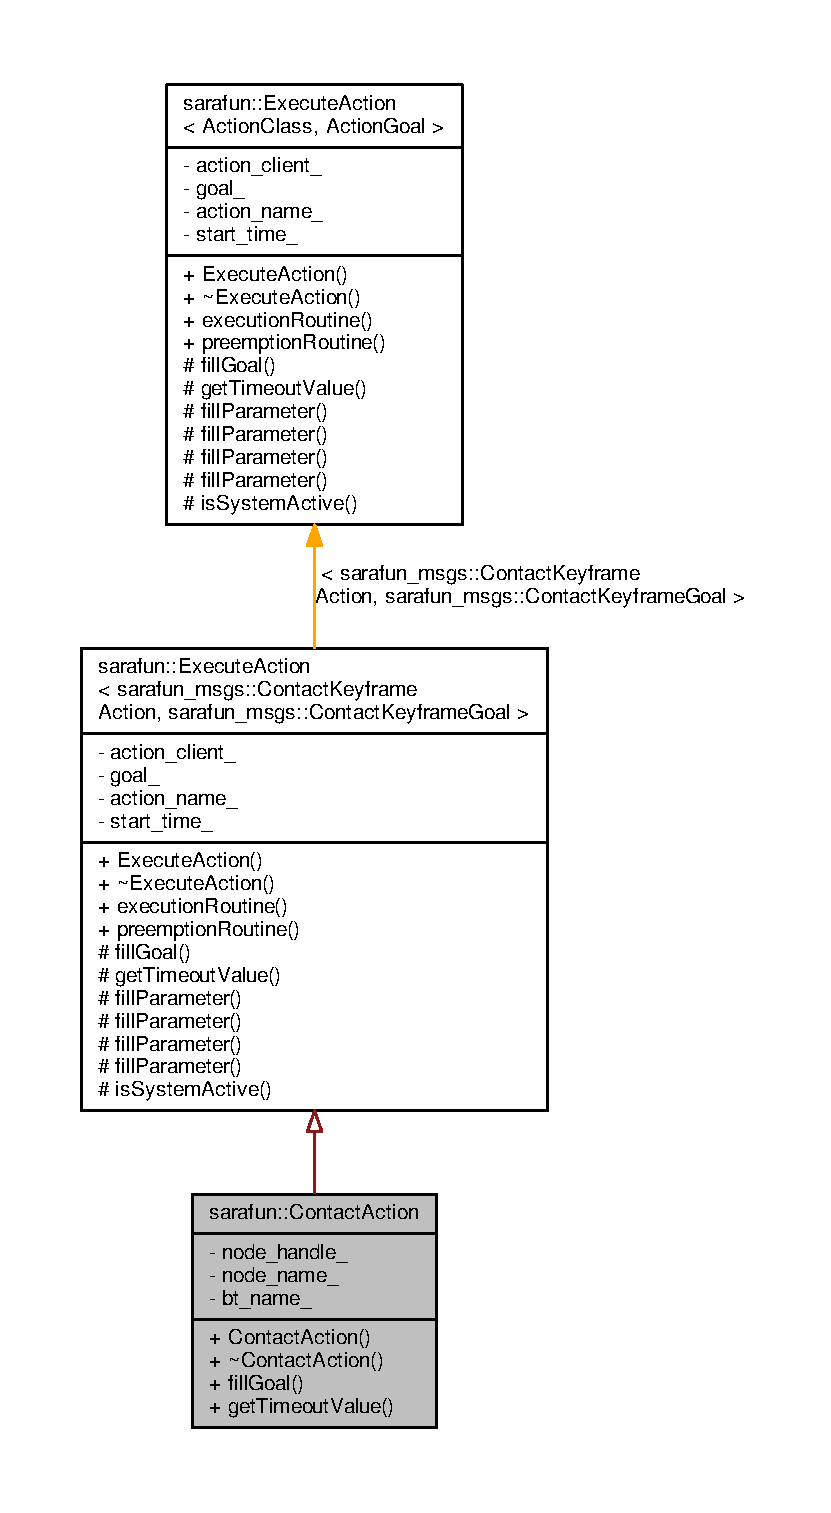
\includegraphics[height=550pt]{d8/d33/classsarafun_1_1ContactAction__inherit__graph}
\end{center}
\end{figure}


Collaboration diagram for sarafun\-:\-:Contact\-Action\-:
\nopagebreak
\begin{figure}[H]
\begin{center}
\leavevmode
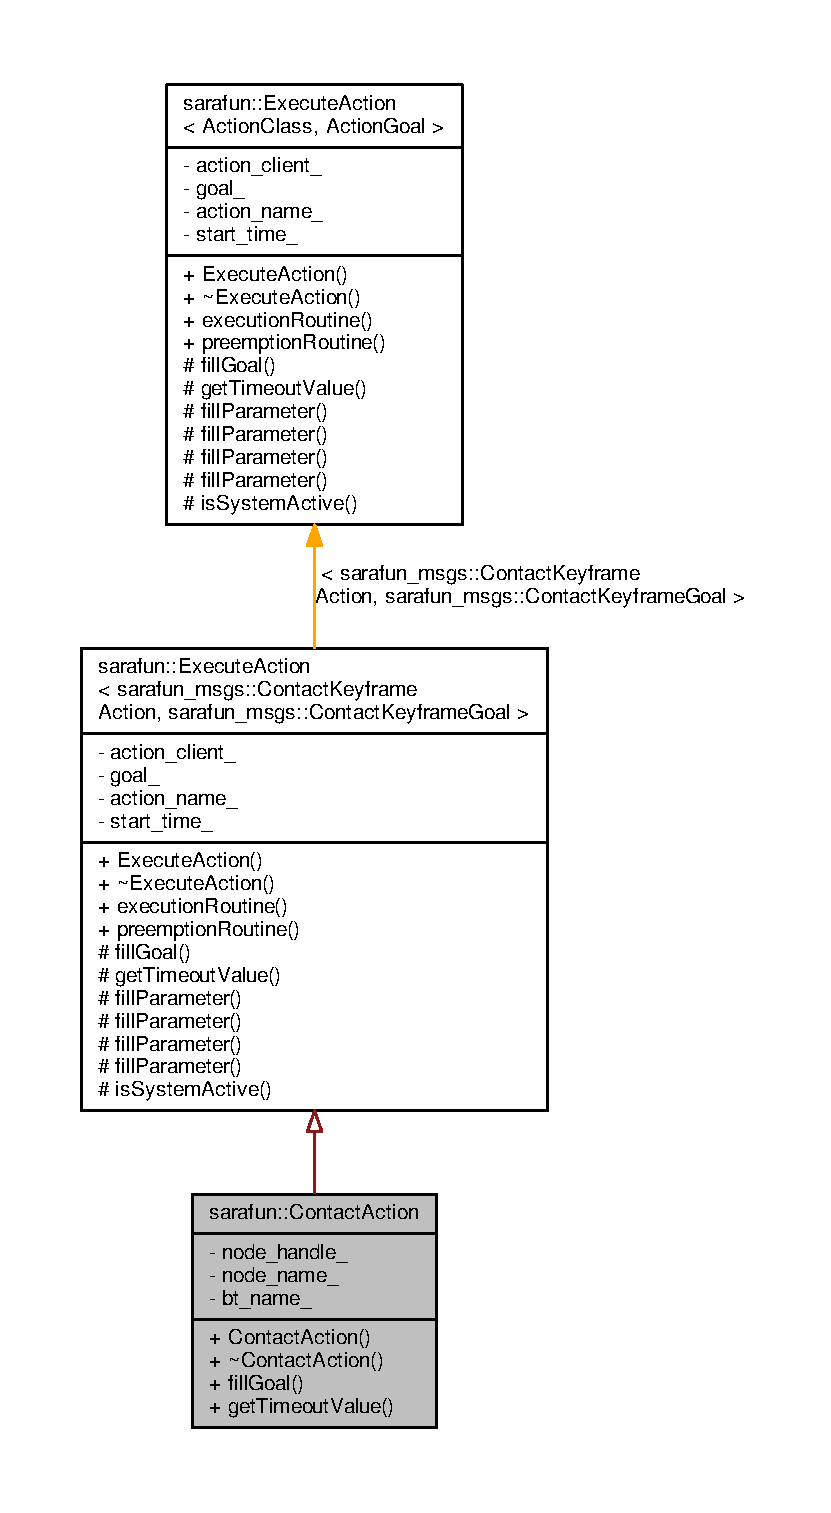
\includegraphics[height=550pt]{d3/d7e/classsarafun_1_1ContactAction__coll__graph}
\end{center}
\end{figure}
\subsection*{Public Member Functions}
\begin{DoxyCompactItemize}
\item 
\hyperlink{classsarafun_1_1ContactAction_a8374da0d20d05fe01b86f2090b2c1770_a8374da0d20d05fe01b86f2090b2c1770}{Contact\-Action} (std\-::string node\-\_\-name, std\-::string action\-\_\-name, std\-::string bt\-\_\-name)
\item 
\hyperlink{classsarafun_1_1ContactAction_a22429fcb44fbe815f745b4924ed08f34_a22429fcb44fbe815f745b4924ed08f34}{$\sim$\-Contact\-Action} ()
\item 
bool \hyperlink{classsarafun_1_1ContactAction_a563907411debe223088ef5a34d8c0fb0_a563907411debe223088ef5a34d8c0fb0}{fill\-Goal} (sarafun\-\_\-msgs\-::\-Contact\-Keyframe\-Goal \&goal)
\item 
double \hyperlink{classsarafun_1_1ContactAction_a85d81232d228fc6d2856d318d25c1bf9_a85d81232d228fc6d2856d318d25c1bf9}{get\-Timeout\-Value} ()
\end{DoxyCompactItemize}
\subsection*{Private Attributes}
\begin{DoxyCompactItemize}
\item 
ros\-::\-Node\-Handle \hyperlink{classsarafun_1_1ContactAction_a01f3f5f489242e0ec4add31d46fb8211_a01f3f5f489242e0ec4add31d46fb8211}{node\-\_\-handle\-\_\-}
\item 
std\-::string \hyperlink{classsarafun_1_1ContactAction_a1b1869bbc4525644b0986a0fbade1039_a1b1869bbc4525644b0986a0fbade1039}{node\-\_\-name\-\_\-}
\item 
std\-::string \hyperlink{classsarafun_1_1ContactAction_a71e5d4dc7682ec4dc8ca0b9b83ee214f_a71e5d4dc7682ec4dc8ca0b9b83ee214f}{bt\-\_\-name\-\_\-}
\end{DoxyCompactItemize}
\subsection*{Additional Inherited Members}


\subsection{Detailed Description}


Definition at line 9 of file Contact\-Action.\-h.



\subsection{Constructor \& Destructor Documentation}
\hypertarget{classsarafun_1_1ContactAction_a8374da0d20d05fe01b86f2090b2c1770_a8374da0d20d05fe01b86f2090b2c1770}{\index{sarafun\-::\-Contact\-Action@{sarafun\-::\-Contact\-Action}!Contact\-Action@{Contact\-Action}}
\index{Contact\-Action@{Contact\-Action}!sarafun::ContactAction@{sarafun\-::\-Contact\-Action}}
\subsubsection[{Contact\-Action}]{\setlength{\rightskip}{0pt plus 5cm}sarafun\-::\-Contact\-Action\-::\-Contact\-Action (
\begin{DoxyParamCaption}
\item[{std\-::string}]{node\-\_\-name, }
\item[{std\-::string}]{action\-\_\-name, }
\item[{std\-::string}]{bt\-\_\-name}
\end{DoxyParamCaption}
)\hspace{0.3cm}{\ttfamily [inline]}}}\label{classsarafun_1_1ContactAction_a8374da0d20d05fe01b86f2090b2c1770_a8374da0d20d05fe01b86f2090b2c1770}


Definition at line 13 of file Contact\-Action.\-h.



References node\-\_\-handle\-\_\-.

\hypertarget{classsarafun_1_1ContactAction_a22429fcb44fbe815f745b4924ed08f34_a22429fcb44fbe815f745b4924ed08f34}{\index{sarafun\-::\-Contact\-Action@{sarafun\-::\-Contact\-Action}!$\sim$\-Contact\-Action@{$\sim$\-Contact\-Action}}
\index{$\sim$\-Contact\-Action@{$\sim$\-Contact\-Action}!sarafun::ContactAction@{sarafun\-::\-Contact\-Action}}
\subsubsection[{$\sim$\-Contact\-Action}]{\setlength{\rightskip}{0pt plus 5cm}sarafun\-::\-Contact\-Action\-::$\sim$\-Contact\-Action (
\begin{DoxyParamCaption}
{}
\end{DoxyParamCaption}
)\hspace{0.3cm}{\ttfamily [inline]}}}\label{classsarafun_1_1ContactAction_a22429fcb44fbe815f745b4924ed08f34_a22429fcb44fbe815f745b4924ed08f34}


Definition at line 23 of file Contact\-Action.\-h.



\subsection{Member Function Documentation}
\hypertarget{classsarafun_1_1ContactAction_a563907411debe223088ef5a34d8c0fb0_a563907411debe223088ef5a34d8c0fb0}{\index{sarafun\-::\-Contact\-Action@{sarafun\-::\-Contact\-Action}!fill\-Goal@{fill\-Goal}}
\index{fill\-Goal@{fill\-Goal}!sarafun::ContactAction@{sarafun\-::\-Contact\-Action}}
\subsubsection[{fill\-Goal}]{\setlength{\rightskip}{0pt plus 5cm}bool sarafun\-::\-Contact\-Action\-::fill\-Goal (
\begin{DoxyParamCaption}
\item[{sarafun\-\_\-msgs\-::\-Contact\-Keyframe\-Goal \&}]{goal}
\end{DoxyParamCaption}
)\hspace{0.3cm}{\ttfamily [virtual]}}}\label{classsarafun_1_1ContactAction_a563907411debe223088ef5a34d8c0fb0_a563907411debe223088ef5a34d8c0fb0}
Fills in the goal for a particular action.


\begin{DoxyParams}{Parameters}
{\em goal} & The actionlib goal message of the externally implemented action. \\
\hline
\end{DoxyParams}
\begin{DoxyReturn}{Returns}
False in case of error, true otherwise. 
\end{DoxyReturn}


Implements \hyperlink{classsarafun_1_1ExecuteAction_a6dd9c0f013d15a17d7e7ce8dbe40a436_a6dd9c0f013d15a17d7e7ce8dbe40a436}{sarafun\-::\-Execute\-Action$<$ sarafun\-\_\-msgs\-::\-Contact\-Keyframe\-Action, sarafun\-\_\-msgs\-::\-Contact\-Keyframe\-Goal $>$}.



Definition at line 4 of file Contact\-Action.\-cpp.



References sarafun\-::\-Execute\-Action$<$ sarafun\-\_\-msgs\-::\-Contact\-Keyframe\-Action, sarafun\-\_\-msgs\-::\-Contact\-Keyframe\-Goal $>$\-::fill\-Parameter().



Here is the call graph for this function\-:
\nopagebreak
\begin{figure}[H]
\begin{center}
\leavevmode
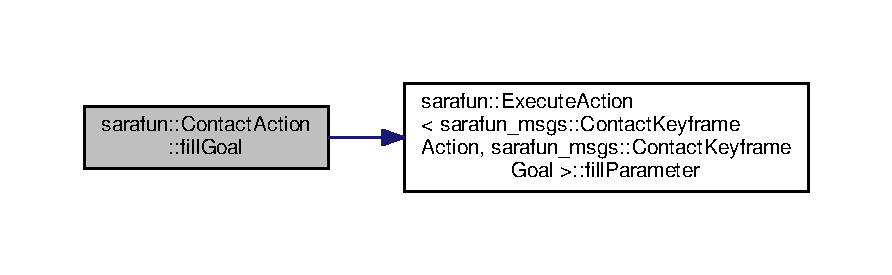
\includegraphics[width=350pt]{dc/d9f/classsarafun_1_1ContactAction_a563907411debe223088ef5a34d8c0fb0_a563907411debe223088ef5a34d8c0fb0_cgraph}
\end{center}
\end{figure}


\hypertarget{classsarafun_1_1ContactAction_a85d81232d228fc6d2856d318d25c1bf9_a85d81232d228fc6d2856d318d25c1bf9}{\index{sarafun\-::\-Contact\-Action@{sarafun\-::\-Contact\-Action}!get\-Timeout\-Value@{get\-Timeout\-Value}}
\index{get\-Timeout\-Value@{get\-Timeout\-Value}!sarafun::ContactAction@{sarafun\-::\-Contact\-Action}}
\subsubsection[{get\-Timeout\-Value}]{\setlength{\rightskip}{0pt plus 5cm}double sarafun\-::\-Contact\-Action\-::get\-Timeout\-Value (
\begin{DoxyParamCaption}
{}
\end{DoxyParamCaption}
)\hspace{0.3cm}{\ttfamily [virtual]}}}\label{classsarafun_1_1ContactAction_a85d81232d228fc6d2856d318d25c1bf9_a85d81232d228fc6d2856d318d25c1bf9}
Provides the client with a timeout value for actionlib connections.

\begin{DoxyReturn}{Returns}
The timeout value (in seconds). 
\end{DoxyReturn}


Implements \hyperlink{classsarafun_1_1ExecuteAction_aba6cfa8a8ce19e735eb6394424df6d17_aba6cfa8a8ce19e735eb6394424df6d17}{sarafun\-::\-Execute\-Action$<$ sarafun\-\_\-msgs\-::\-Contact\-Keyframe\-Action, sarafun\-\_\-msgs\-::\-Contact\-Keyframe\-Goal $>$}.



Definition at line 13 of file Contact\-Action.\-cpp.



References sarafun\-::\-Execute\-Action$<$ sarafun\-\_\-msgs\-::\-Contact\-Keyframe\-Action, sarafun\-\_\-msgs\-::\-Contact\-Keyframe\-Goal $>$\-::fill\-Parameter().



Here is the call graph for this function\-:
\nopagebreak
\begin{figure}[H]
\begin{center}
\leavevmode
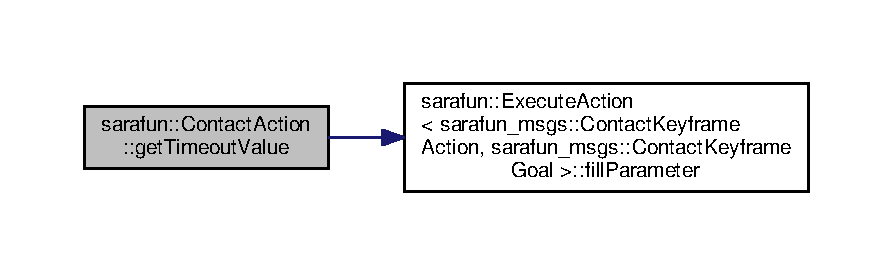
\includegraphics[width=350pt]{dc/d9f/classsarafun_1_1ContactAction_a85d81232d228fc6d2856d318d25c1bf9_a85d81232d228fc6d2856d318d25c1bf9_cgraph}
\end{center}
\end{figure}




\subsection{Field Documentation}
\hypertarget{classsarafun_1_1ContactAction_a71e5d4dc7682ec4dc8ca0b9b83ee214f_a71e5d4dc7682ec4dc8ca0b9b83ee214f}{\index{sarafun\-::\-Contact\-Action@{sarafun\-::\-Contact\-Action}!bt\-\_\-name\-\_\-@{bt\-\_\-name\-\_\-}}
\index{bt\-\_\-name\-\_\-@{bt\-\_\-name\-\_\-}!sarafun::ContactAction@{sarafun\-::\-Contact\-Action}}
\subsubsection[{bt\-\_\-name\-\_\-}]{\setlength{\rightskip}{0pt plus 5cm}std\-::string sarafun\-::\-Contact\-Action\-::bt\-\_\-name\-\_\-\hspace{0.3cm}{\ttfamily [private]}}}\label{classsarafun_1_1ContactAction_a71e5d4dc7682ec4dc8ca0b9b83ee214f_a71e5d4dc7682ec4dc8ca0b9b83ee214f}


Definition at line 31 of file Contact\-Action.\-h.

\hypertarget{classsarafun_1_1ContactAction_a01f3f5f489242e0ec4add31d46fb8211_a01f3f5f489242e0ec4add31d46fb8211}{\index{sarafun\-::\-Contact\-Action@{sarafun\-::\-Contact\-Action}!node\-\_\-handle\-\_\-@{node\-\_\-handle\-\_\-}}
\index{node\-\_\-handle\-\_\-@{node\-\_\-handle\-\_\-}!sarafun::ContactAction@{sarafun\-::\-Contact\-Action}}
\subsubsection[{node\-\_\-handle\-\_\-}]{\setlength{\rightskip}{0pt plus 5cm}ros\-::\-Node\-Handle sarafun\-::\-Contact\-Action\-::node\-\_\-handle\-\_\-\hspace{0.3cm}{\ttfamily [private]}}}\label{classsarafun_1_1ContactAction_a01f3f5f489242e0ec4add31d46fb8211_a01f3f5f489242e0ec4add31d46fb8211}


Definition at line 29 of file Contact\-Action.\-h.



Referenced by Contact\-Action().

\hypertarget{classsarafun_1_1ContactAction_a1b1869bbc4525644b0986a0fbade1039_a1b1869bbc4525644b0986a0fbade1039}{\index{sarafun\-::\-Contact\-Action@{sarafun\-::\-Contact\-Action}!node\-\_\-name\-\_\-@{node\-\_\-name\-\_\-}}
\index{node\-\_\-name\-\_\-@{node\-\_\-name\-\_\-}!sarafun::ContactAction@{sarafun\-::\-Contact\-Action}}
\subsubsection[{node\-\_\-name\-\_\-}]{\setlength{\rightskip}{0pt plus 5cm}std\-::string sarafun\-::\-Contact\-Action\-::node\-\_\-name\-\_\-\hspace{0.3cm}{\ttfamily [private]}}}\label{classsarafun_1_1ContactAction_a1b1869bbc4525644b0986a0fbade1039_a1b1869bbc4525644b0986a0fbade1039}


Definition at line 30 of file Contact\-Action.\-h.



The documentation for this class was generated from the following files\-:\begin{DoxyCompactItemize}
\item 
Contact\-Action.\-h\item 
Contact\-Action.\-cpp\end{DoxyCompactItemize}

\hypertarget{classsarafun_1_1ExecuteAction}{\section{sarafun\-:\-:Execute\-Action$<$ Action\-Class, Action\-Goal $>$ Class Template Reference}
\label{classsarafun_1_1ExecuteAction}\index{sarafun\-::\-Execute\-Action$<$ Action\-Class, Action\-Goal $>$@{sarafun\-::\-Execute\-Action$<$ Action\-Class, Action\-Goal $>$}}
}


{\ttfamily \#include $<$Execute\-Action.\-h$>$}



Inheritance diagram for sarafun\-:\-:Execute\-Action$<$ Action\-Class, Action\-Goal $>$\-:
\nopagebreak
\begin{figure}[H]
\begin{center}
\leavevmode
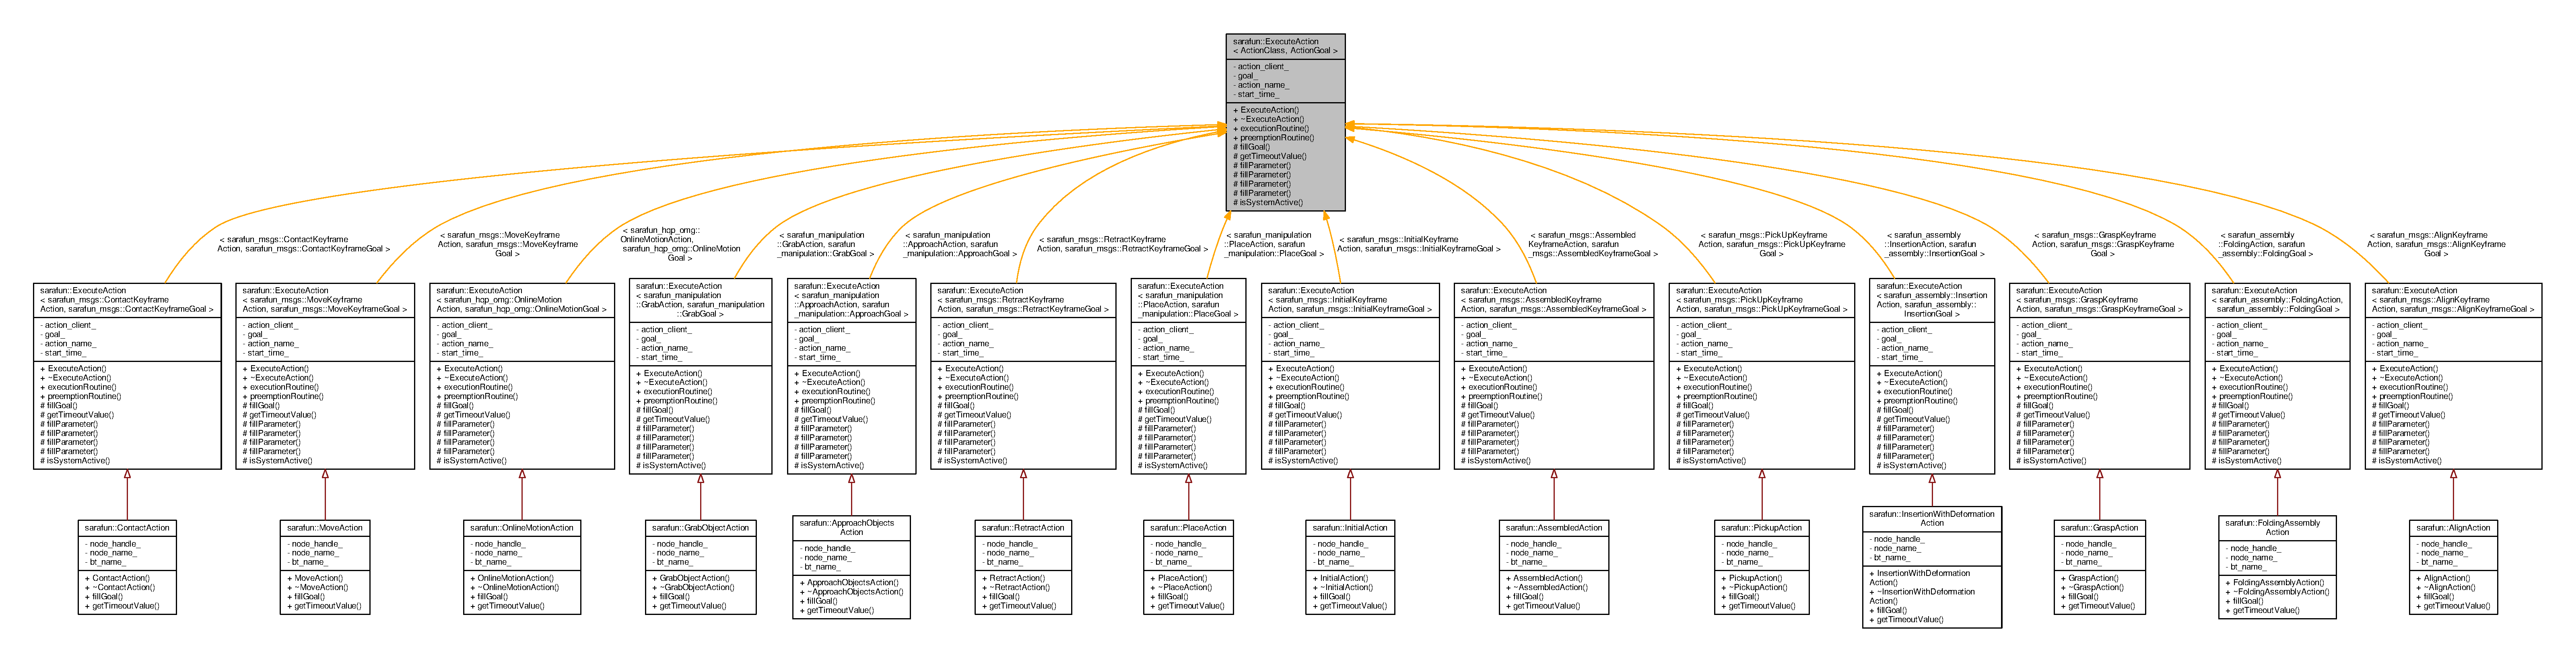
\includegraphics[width=350pt]{db/d30/classsarafun_1_1ExecuteAction__inherit__graph}
\end{center}
\end{figure}


Collaboration diagram for sarafun\-:\-:Execute\-Action$<$ Action\-Class, Action\-Goal $>$\-:
\nopagebreak
\begin{figure}[H]
\begin{center}
\leavevmode
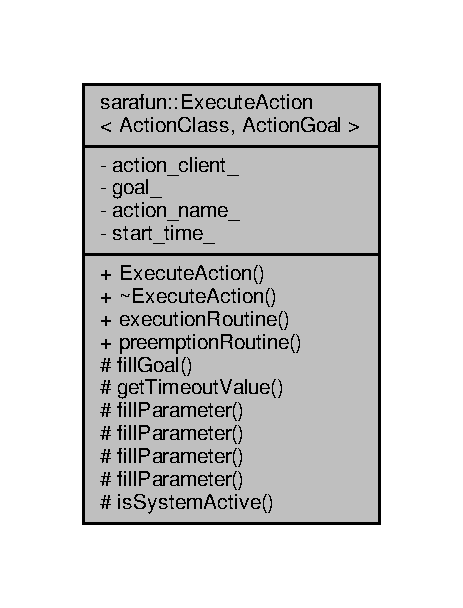
\includegraphics[width=222pt]{de/dc6/classsarafun_1_1ExecuteAction__coll__graph}
\end{center}
\end{figure}
\subsection*{Public Member Functions}
\begin{DoxyCompactItemize}
\item 
\hyperlink{classsarafun_1_1ExecuteAction_acbe4336af2941a52a96aaaceb7e801cb_acbe4336af2941a52a96aaaceb7e801cb}{Execute\-Action} (std\-::string node\-\_\-name, std\-::string actionlib\-\_\-name, std\-::string bt\-\_\-name)
\item 
virtual \hyperlink{classsarafun_1_1ExecuteAction_a194ac46f85d7c70c0aa4f09a0c2941ae_a194ac46f85d7c70c0aa4f09a0c2941ae}{$\sim$\-Execute\-Action} ()
\item 
int \hyperlink{classsarafun_1_1ExecuteAction_ae5e3d1f2779c12923ccdc6289ebba25a_ae5e3d1f2779c12923ccdc6289ebba25a}{execution\-Routine} ()
\item 
void \hyperlink{classsarafun_1_1ExecuteAction_a4075792022071239c6e335c32c70ad2e_a4075792022071239c6e335c32c70ad2e}{preemption\-Routine} ()
\end{DoxyCompactItemize}
\subsection*{Protected Member Functions}
\begin{DoxyCompactItemize}
\item 
virtual bool \hyperlink{classsarafun_1_1ExecuteAction_a6dd9c0f013d15a17d7e7ce8dbe40a436_a6dd9c0f013d15a17d7e7ce8dbe40a436}{fill\-Goal} (Action\-Goal \&goal)=0
\item 
virtual double \hyperlink{classsarafun_1_1ExecuteAction_aba6cfa8a8ce19e735eb6394424df6d17_aba6cfa8a8ce19e735eb6394424df6d17}{get\-Timeout\-Value} ()=0
\item 
bool \hyperlink{classsarafun_1_1ExecuteAction_ac1c8c1ac7392b0ebc8d095d6f6d336e3_ac1c8c1ac7392b0ebc8d095d6f6d336e3}{fill\-Parameter} (std\-::string param\-\_\-name, std\-::string \&param\-\_\-val)
\item 
void \hyperlink{classsarafun_1_1ExecuteAction_a78aa73f154cebe28d4c2fa11ec6a07cf_a78aa73f154cebe28d4c2fa11ec6a07cf}{fill\-Parameter} (std\-::string param\-\_\-name, std\-::string def, std\-::string \&param\-\_\-val)
\item 
void \hyperlink{classsarafun_1_1ExecuteAction_a0c5d656feaf29da583e87f8389570e7d_a0c5d656feaf29da583e87f8389570e7d}{fill\-Parameter} (std\-::string param\-\_\-name, double def, double \&param\-\_\-val)
\item 
void \hyperlink{classsarafun_1_1ExecuteAction_a0ab753300e7535025e7d0508335241a6_a0ab753300e7535025e7d0508335241a6}{fill\-Parameter} (std\-::string param\-\_\-name, int def, int \&param\-\_\-val)
\item 
bool \hyperlink{classsarafun_1_1ExecuteAction_ab9adb2cd743cb8e783fe2a927c94232b_ab9adb2cd743cb8e783fe2a927c94232b}{is\-System\-Active} ()
\end{DoxyCompactItemize}
\subsection*{Private Attributes}
\begin{DoxyCompactItemize}
\item 
actionlib\-::\-Simple\-Action\-Client\\*
$<$ Action\-Class $>$ $\ast$ \hyperlink{classsarafun_1_1ExecuteAction_a8f41836853e5a9daa346b90b865fd113_a8f41836853e5a9daa346b90b865fd113}{action\-\_\-client\-\_\-}
\item 
Action\-Goal \hyperlink{classsarafun_1_1ExecuteAction_a31d3f0c6e50b6abeb68ef6d0cb3c8a4a_a31d3f0c6e50b6abeb68ef6d0cb3c8a4a}{goal\-\_\-}
\item 
std\-::string \hyperlink{classsarafun_1_1ExecuteAction_ac2deed790dd2ff6ef7534fb1a500381f_ac2deed790dd2ff6ef7534fb1a500381f}{action\-\_\-name\-\_\-}
\item 
ros\-::\-Time \hyperlink{classsarafun_1_1ExecuteAction_ad7a81f5e505c421c57bc32fa35e3e84f_ad7a81f5e505c421c57bc32fa35e3e84f}{start\-\_\-time\-\_\-}
\end{DoxyCompactItemize}


\subsection{Detailed Description}
\subsubsection*{template$<$class Action\-Class, class Action\-Goal$>$class sarafun\-::\-Execute\-Action$<$ Action\-Class, Action\-Goal $>$}

This class implements an interface for B\-T actions destined to call a generic rosaction server.

It establishes a bridge between the behavior tree action class and an externally implemented action\-: B\-T $<$--$>$ \hyperlink{classsarafun_1_1ExecuteAction}{Execute\-Action} $<$--$>$ external implementation 

Definition at line 17 of file Execute\-Action.\-h.



\subsection{Constructor \& Destructor Documentation}
\hypertarget{classsarafun_1_1ExecuteAction_acbe4336af2941a52a96aaaceb7e801cb_acbe4336af2941a52a96aaaceb7e801cb}{\index{sarafun\-::\-Execute\-Action@{sarafun\-::\-Execute\-Action}!Execute\-Action@{Execute\-Action}}
\index{Execute\-Action@{Execute\-Action}!sarafun::ExecuteAction@{sarafun\-::\-Execute\-Action}}
\subsubsection[{Execute\-Action}]{\setlength{\rightskip}{0pt plus 5cm}template$<$class Action\-Class , class Action\-Goal $>$ {\bf sarafun\-::\-Execute\-Action}$<$ Action\-Class, Action\-Goal $>$\-::{\bf Execute\-Action} (
\begin{DoxyParamCaption}
\item[{std\-::string}]{node\-\_\-name, }
\item[{std\-::string}]{actionlib\-\_\-name, }
\item[{std\-::string}]{bt\-\_\-name}
\end{DoxyParamCaption}
)}}\label{classsarafun_1_1ExecuteAction_acbe4336af2941a52a96aaaceb7e801cb_acbe4336af2941a52a96aaaceb7e801cb}
Contructor.


\begin{DoxyParams}{Parameters}
{\em node\-\_\-name} & The R\-O\-S node name. \\
\hline
{\em actionlib\-\_\-name} & The actionlib server name that this action will call. \\
\hline
{\em bt\-\_\-name} & The name defined in the \char`\"{}name\char`\"{} tag from the B\-T J\-S\-O\-N input file. \\
\hline
\end{DoxyParams}


Definition at line 90 of file Execute\-Action.\-h.



References sarafun\-::\-Execute\-Action$<$ Action\-Class, Action\-Goal $>$\-::action\-\_\-client\-\_\-, and sarafun\-::\-Execute\-Action$<$ Action\-Class, Action\-Goal $>$\-::action\-\_\-name\-\_\-.

\hypertarget{classsarafun_1_1ExecuteAction_a194ac46f85d7c70c0aa4f09a0c2941ae_a194ac46f85d7c70c0aa4f09a0c2941ae}{\index{sarafun\-::\-Execute\-Action@{sarafun\-::\-Execute\-Action}!$\sim$\-Execute\-Action@{$\sim$\-Execute\-Action}}
\index{$\sim$\-Execute\-Action@{$\sim$\-Execute\-Action}!sarafun::ExecuteAction@{sarafun\-::\-Execute\-Action}}
\subsubsection[{$\sim$\-Execute\-Action}]{\setlength{\rightskip}{0pt plus 5cm}template$<$class Action\-Class , class Action\-Goal $>$ {\bf sarafun\-::\-Execute\-Action}$<$ Action\-Class, Action\-Goal $>$\-::$\sim${\bf Execute\-Action} (
\begin{DoxyParamCaption}
{}
\end{DoxyParamCaption}
)\hspace{0.3cm}{\ttfamily [virtual]}}}\label{classsarafun_1_1ExecuteAction_a194ac46f85d7c70c0aa4f09a0c2941ae_a194ac46f85d7c70c0aa4f09a0c2941ae}


Definition at line 99 of file Execute\-Action.\-h.



\subsection{Member Function Documentation}
\hypertarget{classsarafun_1_1ExecuteAction_ae5e3d1f2779c12923ccdc6289ebba25a_ae5e3d1f2779c12923ccdc6289ebba25a}{\index{sarafun\-::\-Execute\-Action@{sarafun\-::\-Execute\-Action}!execution\-Routine@{execution\-Routine}}
\index{execution\-Routine@{execution\-Routine}!sarafun::ExecuteAction@{sarafun\-::\-Execute\-Action}}
\subsubsection[{execution\-Routine}]{\setlength{\rightskip}{0pt plus 5cm}template$<$class Action\-Class , class Action\-Goal $>$ int {\bf sarafun\-::\-Execute\-Action}$<$ Action\-Class, Action\-Goal $>$\-::execution\-Routine (
\begin{DoxyParamCaption}
{}
\end{DoxyParamCaption}
)}}\label{classsarafun_1_1ExecuteAction_ae5e3d1f2779c12923ccdc6289ebba25a_ae5e3d1f2779c12923ccdc6289ebba25a}


Definition at line 128 of file Execute\-Action.\-h.

\hypertarget{classsarafun_1_1ExecuteAction_a6dd9c0f013d15a17d7e7ce8dbe40a436_a6dd9c0f013d15a17d7e7ce8dbe40a436}{\index{sarafun\-::\-Execute\-Action@{sarafun\-::\-Execute\-Action}!fill\-Goal@{fill\-Goal}}
\index{fill\-Goal@{fill\-Goal}!sarafun::ExecuteAction@{sarafun\-::\-Execute\-Action}}
\subsubsection[{fill\-Goal}]{\setlength{\rightskip}{0pt plus 5cm}template$<$class Action\-Class, class Action\-Goal$>$ virtual bool {\bf sarafun\-::\-Execute\-Action}$<$ Action\-Class, Action\-Goal $>$\-::fill\-Goal (
\begin{DoxyParamCaption}
\item[{Action\-Goal \&}]{goal}
\end{DoxyParamCaption}
)\hspace{0.3cm}{\ttfamily [protected]}, {\ttfamily [pure virtual]}}}\label{classsarafun_1_1ExecuteAction_a6dd9c0f013d15a17d7e7ce8dbe40a436_a6dd9c0f013d15a17d7e7ce8dbe40a436}
Fills in the goal for a particular action.


\begin{DoxyParams}{Parameters}
{\em goal} & The actionlib goal message of the externally implemented action. \\
\hline
\end{DoxyParams}
\begin{DoxyReturn}{Returns}
False in case of error, true otherwise. 
\end{DoxyReturn}


Implemented in \hyperlink{classsarafun_1_1ApproachObjectsAction_af5d216551122da780bc550daf4f1dca4_af5d216551122da780bc550daf4f1dca4}{sarafun\-::\-Approach\-Objects\-Action}, \hyperlink{classsarafun_1_1InsertionWithDeformationAction_a32d695dfcd626c5a7ca0fa987c245083_a32d695dfcd626c5a7ca0fa987c245083}{sarafun\-::\-Insertion\-With\-Deformation\-Action}, \hyperlink{classsarafun_1_1AlignAction_ab92a62085ebd60438638b7b6c56da786_ab92a62085ebd60438638b7b6c56da786}{sarafun\-::\-Align\-Action}, \hyperlink{classsarafun_1_1AssembledAction_a094a5cfde4d6bb6d024256834e771a39_a094a5cfde4d6bb6d024256834e771a39}{sarafun\-::\-Assembled\-Action}, \hyperlink{classsarafun_1_1ContactAction_a563907411debe223088ef5a34d8c0fb0_a563907411debe223088ef5a34d8c0fb0}{sarafun\-::\-Contact\-Action}, \hyperlink{classsarafun_1_1GraspAction_a7418fe9de5024a8fbbfe8e5f5336d66f_a7418fe9de5024a8fbbfe8e5f5336d66f}{sarafun\-::\-Grasp\-Action}, \hyperlink{classsarafun_1_1InitialAction_aac7f439c30455349e075e91542565a43_aac7f439c30455349e075e91542565a43}{sarafun\-::\-Initial\-Action}, \hyperlink{classsarafun_1_1MoveAction_ad5259389b6a5718389c24fab920c9296_ad5259389b6a5718389c24fab920c9296}{sarafun\-::\-Move\-Action}, \hyperlink{classsarafun_1_1PickupAction_a4aa9956733de9f12b52aa41038dbe87a_a4aa9956733de9f12b52aa41038dbe87a}{sarafun\-::\-Pickup\-Action}, \hyperlink{classsarafun_1_1RetractAction_ad0db1c2615d68603bc972ffa26049a70_ad0db1c2615d68603bc972ffa26049a70}{sarafun\-::\-Retract\-Action}, \hyperlink{classsarafun_1_1GrabObjectAction_a61fe8b0cb93dec244f10d6c5dbee913c_a61fe8b0cb93dec244f10d6c5dbee913c}{sarafun\-::\-Grab\-Object\-Action}, \hyperlink{classsarafun_1_1OnlineMotionAction_aacaa264dad7ba07b5c9a985d66ea48f7_aacaa264dad7ba07b5c9a985d66ea48f7}{sarafun\-::\-Online\-Motion\-Action}, \hyperlink{classsarafun_1_1PlaceAction_a7d48e758adf6cea93fa15409bafda8c8_a7d48e758adf6cea93fa15409bafda8c8}{sarafun\-::\-Place\-Action}, and \hyperlink{classsarafun_1_1FoldingAssemblyAction_a51597860319456f359d03c3e27c2fb96_a51597860319456f359d03c3e27c2fb96}{sarafun\-::\-Folding\-Assembly\-Action}.

\hypertarget{classsarafun_1_1ExecuteAction_ac1c8c1ac7392b0ebc8d095d6f6d336e3_ac1c8c1ac7392b0ebc8d095d6f6d336e3}{\index{sarafun\-::\-Execute\-Action@{sarafun\-::\-Execute\-Action}!fill\-Parameter@{fill\-Parameter}}
\index{fill\-Parameter@{fill\-Parameter}!sarafun::ExecuteAction@{sarafun\-::\-Execute\-Action}}
\subsubsection[{fill\-Parameter}]{\setlength{\rightskip}{0pt plus 5cm}template$<$class Action\-Class , class Action\-Goal $>$ bool {\bf sarafun\-::\-Execute\-Action}$<$ Action\-Class, Action\-Goal $>$\-::fill\-Parameter (
\begin{DoxyParamCaption}
\item[{std\-::string}]{param\-\_\-name, }
\item[{std\-::string \&}]{param\-\_\-val}
\end{DoxyParamCaption}
)\hspace{0.3cm}{\ttfamily [protected]}}}\label{classsarafun_1_1ExecuteAction_ac1c8c1ac7392b0ebc8d095d6f6d336e3_ac1c8c1ac7392b0ebc8d095d6f6d336e3}
Gets generic parameter from the parameter server.


\begin{DoxyParams}{Parameters}
{\em The} & parameter name.  The parameter value. \\
\hline
\end{DoxyParams}
\begin{DoxyReturn}{Returns}
False in case the parameter does not exist, true otherise. 
\end{DoxyReturn}


Definition at line 198 of file Execute\-Action.\-h.

\hypertarget{classsarafun_1_1ExecuteAction_a78aa73f154cebe28d4c2fa11ec6a07cf_a78aa73f154cebe28d4c2fa11ec6a07cf}{\index{sarafun\-::\-Execute\-Action@{sarafun\-::\-Execute\-Action}!fill\-Parameter@{fill\-Parameter}}
\index{fill\-Parameter@{fill\-Parameter}!sarafun::ExecuteAction@{sarafun\-::\-Execute\-Action}}
\subsubsection[{fill\-Parameter}]{\setlength{\rightskip}{0pt plus 5cm}template$<$class Action\-Class , class Action\-Goal $>$ void {\bf sarafun\-::\-Execute\-Action}$<$ Action\-Class, Action\-Goal $>$\-::fill\-Parameter (
\begin{DoxyParamCaption}
\item[{std\-::string}]{param\-\_\-name, }
\item[{std\-::string}]{def, }
\item[{std\-::string \&}]{param\-\_\-val}
\end{DoxyParamCaption}
)\hspace{0.3cm}{\ttfamily [protected]}}}\label{classsarafun_1_1ExecuteAction_a78aa73f154cebe28d4c2fa11ec6a07cf_a78aa73f154cebe28d4c2fa11ec6a07cf}
Gets a generic parameter from the parameter server. Sets it to a default in case the parameter does not exist.


\begin{DoxyParams}{Parameters}
{\em The} & parameter name \\
\hline
{\em def} & The default parameter value  The parameter value \\
\hline
\end{DoxyParams}


Definition at line 210 of file Execute\-Action.\-h.

\hypertarget{classsarafun_1_1ExecuteAction_a0c5d656feaf29da583e87f8389570e7d_a0c5d656feaf29da583e87f8389570e7d}{\index{sarafun\-::\-Execute\-Action@{sarafun\-::\-Execute\-Action}!fill\-Parameter@{fill\-Parameter}}
\index{fill\-Parameter@{fill\-Parameter}!sarafun::ExecuteAction@{sarafun\-::\-Execute\-Action}}
\subsubsection[{fill\-Parameter}]{\setlength{\rightskip}{0pt plus 5cm}template$<$class Action\-Class , class Action\-Goal $>$ void {\bf sarafun\-::\-Execute\-Action}$<$ Action\-Class, Action\-Goal $>$\-::fill\-Parameter (
\begin{DoxyParamCaption}
\item[{std\-::string}]{param\-\_\-name, }
\item[{double}]{def, }
\item[{double \&}]{param\-\_\-val}
\end{DoxyParamCaption}
)\hspace{0.3cm}{\ttfamily [protected]}}}\label{classsarafun_1_1ExecuteAction_a0c5d656feaf29da583e87f8389570e7d_a0c5d656feaf29da583e87f8389570e7d}


Definition at line 221 of file Execute\-Action.\-h.

\hypertarget{classsarafun_1_1ExecuteAction_a0ab753300e7535025e7d0508335241a6_a0ab753300e7535025e7d0508335241a6}{\index{sarafun\-::\-Execute\-Action@{sarafun\-::\-Execute\-Action}!fill\-Parameter@{fill\-Parameter}}
\index{fill\-Parameter@{fill\-Parameter}!sarafun::ExecuteAction@{sarafun\-::\-Execute\-Action}}
\subsubsection[{fill\-Parameter}]{\setlength{\rightskip}{0pt plus 5cm}template$<$class Action\-Class , class Action\-Goal $>$ void {\bf sarafun\-::\-Execute\-Action}$<$ Action\-Class, Action\-Goal $>$\-::fill\-Parameter (
\begin{DoxyParamCaption}
\item[{std\-::string}]{param\-\_\-name, }
\item[{int}]{def, }
\item[{int \&}]{param\-\_\-val}
\end{DoxyParamCaption}
)\hspace{0.3cm}{\ttfamily [protected]}}}\label{classsarafun_1_1ExecuteAction_a0ab753300e7535025e7d0508335241a6_a0ab753300e7535025e7d0508335241a6}


Definition at line 232 of file Execute\-Action.\-h.

\hypertarget{classsarafun_1_1ExecuteAction_aba6cfa8a8ce19e735eb6394424df6d17_aba6cfa8a8ce19e735eb6394424df6d17}{\index{sarafun\-::\-Execute\-Action@{sarafun\-::\-Execute\-Action}!get\-Timeout\-Value@{get\-Timeout\-Value}}
\index{get\-Timeout\-Value@{get\-Timeout\-Value}!sarafun::ExecuteAction@{sarafun\-::\-Execute\-Action}}
\subsubsection[{get\-Timeout\-Value}]{\setlength{\rightskip}{0pt plus 5cm}template$<$class Action\-Class, class Action\-Goal$>$ virtual double {\bf sarafun\-::\-Execute\-Action}$<$ Action\-Class, Action\-Goal $>$\-::get\-Timeout\-Value (
\begin{DoxyParamCaption}
{}
\end{DoxyParamCaption}
)\hspace{0.3cm}{\ttfamily [protected]}, {\ttfamily [pure virtual]}}}\label{classsarafun_1_1ExecuteAction_aba6cfa8a8ce19e735eb6394424df6d17_aba6cfa8a8ce19e735eb6394424df6d17}
Provides the client with a timeout value for actionlib connections.

\begin{DoxyReturn}{Returns}
The timeout value (in seconds). 
\end{DoxyReturn}


Implemented in \hyperlink{classsarafun_1_1ApproachObjectsAction_a6852994a6e8a1edf9b2c24c91fd07df2_a6852994a6e8a1edf9b2c24c91fd07df2}{sarafun\-::\-Approach\-Objects\-Action}, \hyperlink{classsarafun_1_1InsertionWithDeformationAction_a8d77b104fb2396000b273cb6754ff879_a8d77b104fb2396000b273cb6754ff879}{sarafun\-::\-Insertion\-With\-Deformation\-Action}, \hyperlink{classsarafun_1_1AlignAction_a9b9741ec3203bdc1b2e7b7cecc96e6ed_a9b9741ec3203bdc1b2e7b7cecc96e6ed}{sarafun\-::\-Align\-Action}, \hyperlink{classsarafun_1_1AssembledAction_ade9095a291dce652339238d137419b49_ade9095a291dce652339238d137419b49}{sarafun\-::\-Assembled\-Action}, \hyperlink{classsarafun_1_1ContactAction_a85d81232d228fc6d2856d318d25c1bf9_a85d81232d228fc6d2856d318d25c1bf9}{sarafun\-::\-Contact\-Action}, \hyperlink{classsarafun_1_1GraspAction_a406d5c86b5f788537c5af9d125724a55_a406d5c86b5f788537c5af9d125724a55}{sarafun\-::\-Grasp\-Action}, \hyperlink{classsarafun_1_1InitialAction_a1b58c06c32ec9f9d3e75c37de5e7d2c8_a1b58c06c32ec9f9d3e75c37de5e7d2c8}{sarafun\-::\-Initial\-Action}, \hyperlink{classsarafun_1_1MoveAction_a3a0d4d2919b30b878c603a884db6a470_a3a0d4d2919b30b878c603a884db6a470}{sarafun\-::\-Move\-Action}, \hyperlink{classsarafun_1_1PickupAction_a02643cdc836095102e5622b660233f26_a02643cdc836095102e5622b660233f26}{sarafun\-::\-Pickup\-Action}, \hyperlink{classsarafun_1_1RetractAction_af95bb8d3826dbe1444a8a3e12d8596b0_af95bb8d3826dbe1444a8a3e12d8596b0}{sarafun\-::\-Retract\-Action}, \hyperlink{classsarafun_1_1GrabObjectAction_a6e2ee834fda8bd8d0dbdc101c8acdd9c_a6e2ee834fda8bd8d0dbdc101c8acdd9c}{sarafun\-::\-Grab\-Object\-Action}, \hyperlink{classsarafun_1_1OnlineMotionAction_a453e7dca41a0d73b5297ce191e760b31_a453e7dca41a0d73b5297ce191e760b31}{sarafun\-::\-Online\-Motion\-Action}, \hyperlink{classsarafun_1_1PlaceAction_a0b53372fd2de920c3ebd94c8c7f80b6a_a0b53372fd2de920c3ebd94c8c7f80b6a}{sarafun\-::\-Place\-Action}, and \hyperlink{classsarafun_1_1FoldingAssemblyAction_a14174e375aa1b8d5b63159f275b7d971_a14174e375aa1b8d5b63159f275b7d971}{sarafun\-::\-Folding\-Assembly\-Action}.

\hypertarget{classsarafun_1_1ExecuteAction_ab9adb2cd743cb8e783fe2a927c94232b_ab9adb2cd743cb8e783fe2a927c94232b}{\index{sarafun\-::\-Execute\-Action@{sarafun\-::\-Execute\-Action}!is\-System\-Active@{is\-System\-Active}}
\index{is\-System\-Active@{is\-System\-Active}!sarafun::ExecuteAction@{sarafun\-::\-Execute\-Action}}
\subsubsection[{is\-System\-Active}]{\setlength{\rightskip}{0pt plus 5cm}template$<$class Action\-Class , class Action\-Goal $>$ bool {\bf sarafun\-::\-Execute\-Action}$<$ Action\-Class, Action\-Goal $>$\-::is\-System\-Active (
\begin{DoxyParamCaption}
{}
\end{DoxyParamCaption}
)\hspace{0.3cm}{\ttfamily [protected]}}}\label{classsarafun_1_1ExecuteAction_ab9adb2cd743cb8e783fe2a927c94232b_ab9adb2cd743cb8e783fe2a927c94232b}
Checks if B\-T action execution is allowed.

\begin{DoxyReturn}{Returns}
True if the tree is active, false otherwise. 
\end{DoxyReturn}


Definition at line 104 of file Execute\-Action.\-h.

\hypertarget{classsarafun_1_1ExecuteAction_a4075792022071239c6e335c32c70ad2e_a4075792022071239c6e335c32c70ad2e}{\index{sarafun\-::\-Execute\-Action@{sarafun\-::\-Execute\-Action}!preemption\-Routine@{preemption\-Routine}}
\index{preemption\-Routine@{preemption\-Routine}!sarafun::ExecuteAction@{sarafun\-::\-Execute\-Action}}
\subsubsection[{preemption\-Routine}]{\setlength{\rightskip}{0pt plus 5cm}template$<$class Action\-Class , class Action\-Goal $>$ void {\bf sarafun\-::\-Execute\-Action}$<$ Action\-Class, Action\-Goal $>$\-::preemption\-Routine (
\begin{DoxyParamCaption}
{}
\end{DoxyParamCaption}
)}}\label{classsarafun_1_1ExecuteAction_a4075792022071239c6e335c32c70ad2e_a4075792022071239c6e335c32c70ad2e}


Definition at line 120 of file Execute\-Action.\-h.



\subsection{Field Documentation}
\hypertarget{classsarafun_1_1ExecuteAction_a8f41836853e5a9daa346b90b865fd113_a8f41836853e5a9daa346b90b865fd113}{\index{sarafun\-::\-Execute\-Action@{sarafun\-::\-Execute\-Action}!action\-\_\-client\-\_\-@{action\-\_\-client\-\_\-}}
\index{action\-\_\-client\-\_\-@{action\-\_\-client\-\_\-}!sarafun::ExecuteAction@{sarafun\-::\-Execute\-Action}}
\subsubsection[{action\-\_\-client\-\_\-}]{\setlength{\rightskip}{0pt plus 5cm}template$<$class Action\-Class, class Action\-Goal$>$ actionlib\-::\-Simple\-Action\-Client$<$Action\-Class$>$$\ast$ {\bf sarafun\-::\-Execute\-Action}$<$ Action\-Class, Action\-Goal $>$\-::action\-\_\-client\-\_\-\hspace{0.3cm}{\ttfamily [private]}}}\label{classsarafun_1_1ExecuteAction_a8f41836853e5a9daa346b90b865fd113_a8f41836853e5a9daa346b90b865fd113}


Definition at line 80 of file Execute\-Action.\-h.



Referenced by sarafun\-::\-Execute\-Action$<$ Action\-Class, Action\-Goal $>$\-::\-Execute\-Action().

\hypertarget{classsarafun_1_1ExecuteAction_ac2deed790dd2ff6ef7534fb1a500381f_ac2deed790dd2ff6ef7534fb1a500381f}{\index{sarafun\-::\-Execute\-Action@{sarafun\-::\-Execute\-Action}!action\-\_\-name\-\_\-@{action\-\_\-name\-\_\-}}
\index{action\-\_\-name\-\_\-@{action\-\_\-name\-\_\-}!sarafun::ExecuteAction@{sarafun\-::\-Execute\-Action}}
\subsubsection[{action\-\_\-name\-\_\-}]{\setlength{\rightskip}{0pt plus 5cm}template$<$class Action\-Class, class Action\-Goal$>$ std\-::string {\bf sarafun\-::\-Execute\-Action}$<$ Action\-Class, Action\-Goal $>$\-::action\-\_\-name\-\_\-\hspace{0.3cm}{\ttfamily [private]}}}\label{classsarafun_1_1ExecuteAction_ac2deed790dd2ff6ef7534fb1a500381f_ac2deed790dd2ff6ef7534fb1a500381f}


Definition at line 82 of file Execute\-Action.\-h.



Referenced by sarafun\-::\-Execute\-Action$<$ Action\-Class, Action\-Goal $>$\-::\-Execute\-Action().

\hypertarget{classsarafun_1_1ExecuteAction_a31d3f0c6e50b6abeb68ef6d0cb3c8a4a_a31d3f0c6e50b6abeb68ef6d0cb3c8a4a}{\index{sarafun\-::\-Execute\-Action@{sarafun\-::\-Execute\-Action}!goal\-\_\-@{goal\-\_\-}}
\index{goal\-\_\-@{goal\-\_\-}!sarafun::ExecuteAction@{sarafun\-::\-Execute\-Action}}
\subsubsection[{goal\-\_\-}]{\setlength{\rightskip}{0pt plus 5cm}template$<$class Action\-Class, class Action\-Goal$>$ Action\-Goal {\bf sarafun\-::\-Execute\-Action}$<$ Action\-Class, Action\-Goal $>$\-::goal\-\_\-\hspace{0.3cm}{\ttfamily [private]}}}\label{classsarafun_1_1ExecuteAction_a31d3f0c6e50b6abeb68ef6d0cb3c8a4a_a31d3f0c6e50b6abeb68ef6d0cb3c8a4a}


Definition at line 81 of file Execute\-Action.\-h.

\hypertarget{classsarafun_1_1ExecuteAction_ad7a81f5e505c421c57bc32fa35e3e84f_ad7a81f5e505c421c57bc32fa35e3e84f}{\index{sarafun\-::\-Execute\-Action@{sarafun\-::\-Execute\-Action}!start\-\_\-time\-\_\-@{start\-\_\-time\-\_\-}}
\index{start\-\_\-time\-\_\-@{start\-\_\-time\-\_\-}!sarafun::ExecuteAction@{sarafun\-::\-Execute\-Action}}
\subsubsection[{start\-\_\-time\-\_\-}]{\setlength{\rightskip}{0pt plus 5cm}template$<$class Action\-Class, class Action\-Goal$>$ ros\-::\-Time {\bf sarafun\-::\-Execute\-Action}$<$ Action\-Class, Action\-Goal $>$\-::start\-\_\-time\-\_\-\hspace{0.3cm}{\ttfamily [private]}}}\label{classsarafun_1_1ExecuteAction_ad7a81f5e505c421c57bc32fa35e3e84f_ad7a81f5e505c421c57bc32fa35e3e84f}


Definition at line 83 of file Execute\-Action.\-h.



The documentation for this class was generated from the following file\-:\begin{DoxyCompactItemize}
\item 
Execute\-Action.\-h\end{DoxyCompactItemize}

\hypertarget{classsarafun_1_1FoldingAssemblyAction}{\section{sarafun\-:\-:Folding\-Assembly\-Action Class Reference}
\label{classsarafun_1_1FoldingAssemblyAction}\index{sarafun\-::\-Folding\-Assembly\-Action@{sarafun\-::\-Folding\-Assembly\-Action}}
}


{\ttfamily \#include $<$Folding\-Assembly\-Action.\-h$>$}



Inheritance diagram for sarafun\-:\-:Folding\-Assembly\-Action\-:
\nopagebreak
\begin{figure}[H]
\begin{center}
\leavevmode
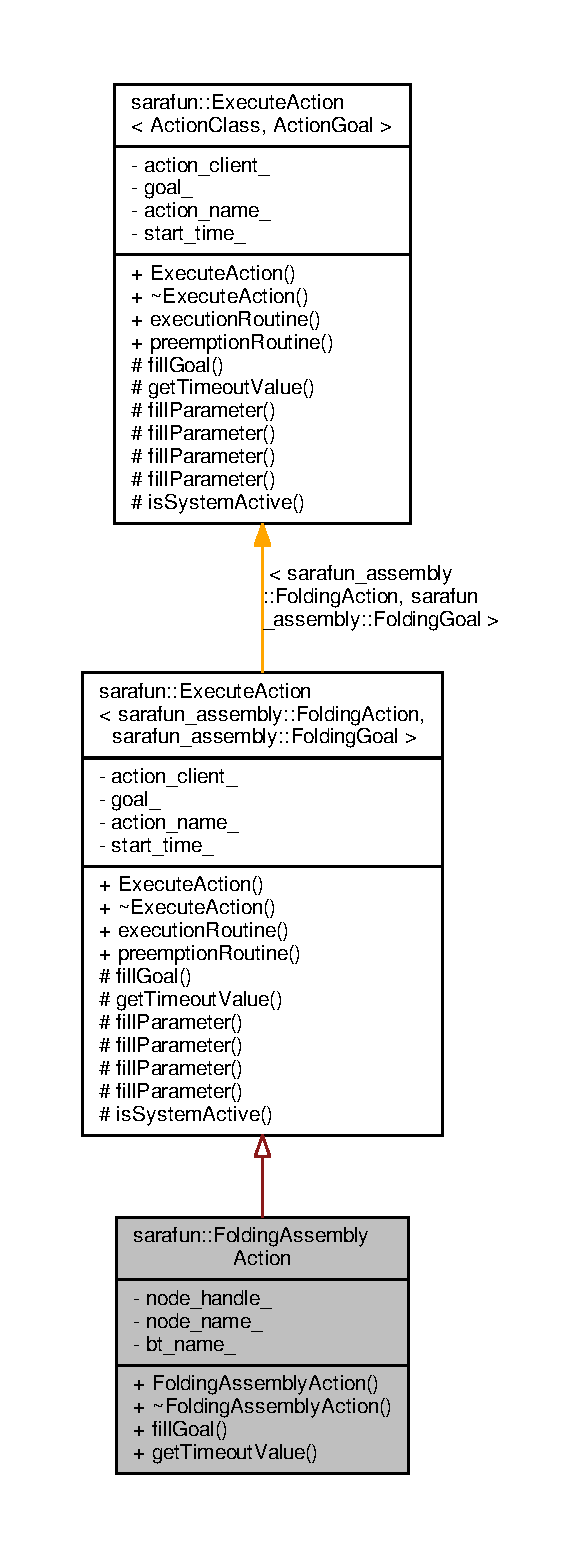
\includegraphics[height=550pt]{d3/d87/classsarafun_1_1FoldingAssemblyAction__inherit__graph}
\end{center}
\end{figure}


Collaboration diagram for sarafun\-:\-:Folding\-Assembly\-Action\-:
\nopagebreak
\begin{figure}[H]
\begin{center}
\leavevmode
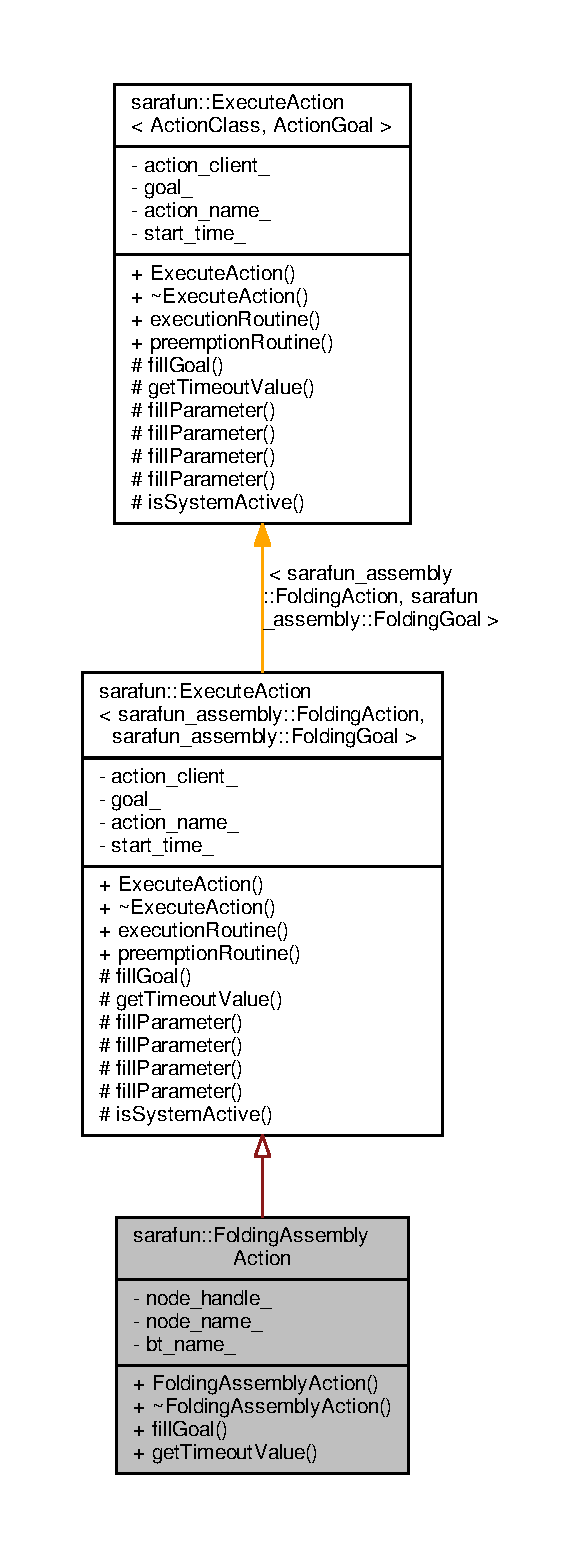
\includegraphics[height=550pt]{de/d2e/classsarafun_1_1FoldingAssemblyAction__coll__graph}
\end{center}
\end{figure}
\subsection*{Public Member Functions}
\begin{DoxyCompactItemize}
\item 
\hyperlink{classsarafun_1_1FoldingAssemblyAction_afc2da251f362a62c892f41d8e0bea0e5_afc2da251f362a62c892f41d8e0bea0e5}{Folding\-Assembly\-Action} (std\-::string node\-\_\-name, std\-::string action\-\_\-name, std\-::string bt\-\_\-name)
\item 
\hyperlink{classsarafun_1_1FoldingAssemblyAction_a0e38e473ec7b9327dc0a4d32e11cc0d6_a0e38e473ec7b9327dc0a4d32e11cc0d6}{$\sim$\-Folding\-Assembly\-Action} ()
\item 
bool \hyperlink{classsarafun_1_1FoldingAssemblyAction_a51597860319456f359d03c3e27c2fb96_a51597860319456f359d03c3e27c2fb96}{fill\-Goal} (sarafun\-\_\-assembly\-::\-Folding\-Goal \&goal)
\item 
double \hyperlink{classsarafun_1_1FoldingAssemblyAction_a14174e375aa1b8d5b63159f275b7d971_a14174e375aa1b8d5b63159f275b7d971}{get\-Timeout\-Value} ()
\end{DoxyCompactItemize}
\subsection*{Private Attributes}
\begin{DoxyCompactItemize}
\item 
ros\-::\-Node\-Handle \hyperlink{classsarafun_1_1FoldingAssemblyAction_a93ef41f7c8fe0fff59227e01deae7625_a93ef41f7c8fe0fff59227e01deae7625}{node\-\_\-handle\-\_\-}
\item 
std\-::string \hyperlink{classsarafun_1_1FoldingAssemblyAction_a80098bc35b0c446a61b0e84f4e97c8ab_a80098bc35b0c446a61b0e84f4e97c8ab}{node\-\_\-name\-\_\-}
\item 
std\-::string \hyperlink{classsarafun_1_1FoldingAssemblyAction_a058ad644052e931e604053b6064f7576_a058ad644052e931e604053b6064f7576}{bt\-\_\-name\-\_\-}
\end{DoxyCompactItemize}
\subsection*{Additional Inherited Members}


\subsection{Detailed Description}


Definition at line 9 of file Folding\-Assembly\-Action.\-h.



\subsection{Constructor \& Destructor Documentation}
\hypertarget{classsarafun_1_1FoldingAssemblyAction_afc2da251f362a62c892f41d8e0bea0e5_afc2da251f362a62c892f41d8e0bea0e5}{\index{sarafun\-::\-Folding\-Assembly\-Action@{sarafun\-::\-Folding\-Assembly\-Action}!Folding\-Assembly\-Action@{Folding\-Assembly\-Action}}
\index{Folding\-Assembly\-Action@{Folding\-Assembly\-Action}!sarafun::FoldingAssemblyAction@{sarafun\-::\-Folding\-Assembly\-Action}}
\subsubsection[{Folding\-Assembly\-Action}]{\setlength{\rightskip}{0pt plus 5cm}sarafun\-::\-Folding\-Assembly\-Action\-::\-Folding\-Assembly\-Action (
\begin{DoxyParamCaption}
\item[{std\-::string}]{node\-\_\-name, }
\item[{std\-::string}]{action\-\_\-name, }
\item[{std\-::string}]{bt\-\_\-name}
\end{DoxyParamCaption}
)\hspace{0.3cm}{\ttfamily [inline]}}}\label{classsarafun_1_1FoldingAssemblyAction_afc2da251f362a62c892f41d8e0bea0e5_afc2da251f362a62c892f41d8e0bea0e5}


Definition at line 12 of file Folding\-Assembly\-Action.\-h.



References node\-\_\-handle\-\_\-.

\hypertarget{classsarafun_1_1FoldingAssemblyAction_a0e38e473ec7b9327dc0a4d32e11cc0d6_a0e38e473ec7b9327dc0a4d32e11cc0d6}{\index{sarafun\-::\-Folding\-Assembly\-Action@{sarafun\-::\-Folding\-Assembly\-Action}!$\sim$\-Folding\-Assembly\-Action@{$\sim$\-Folding\-Assembly\-Action}}
\index{$\sim$\-Folding\-Assembly\-Action@{$\sim$\-Folding\-Assembly\-Action}!sarafun::FoldingAssemblyAction@{sarafun\-::\-Folding\-Assembly\-Action}}
\subsubsection[{$\sim$\-Folding\-Assembly\-Action}]{\setlength{\rightskip}{0pt plus 5cm}sarafun\-::\-Folding\-Assembly\-Action\-::$\sim$\-Folding\-Assembly\-Action (
\begin{DoxyParamCaption}
{}
\end{DoxyParamCaption}
)\hspace{0.3cm}{\ttfamily [inline]}}}\label{classsarafun_1_1FoldingAssemblyAction_a0e38e473ec7b9327dc0a4d32e11cc0d6_a0e38e473ec7b9327dc0a4d32e11cc0d6}


Definition at line 21 of file Folding\-Assembly\-Action.\-h.



\subsection{Member Function Documentation}
\hypertarget{classsarafun_1_1FoldingAssemblyAction_a51597860319456f359d03c3e27c2fb96_a51597860319456f359d03c3e27c2fb96}{\index{sarafun\-::\-Folding\-Assembly\-Action@{sarafun\-::\-Folding\-Assembly\-Action}!fill\-Goal@{fill\-Goal}}
\index{fill\-Goal@{fill\-Goal}!sarafun::FoldingAssemblyAction@{sarafun\-::\-Folding\-Assembly\-Action}}
\subsubsection[{fill\-Goal}]{\setlength{\rightskip}{0pt plus 5cm}bool sarafun\-::\-Folding\-Assembly\-Action\-::fill\-Goal (
\begin{DoxyParamCaption}
\item[{sarafun\-\_\-assembly\-::\-Folding\-Goal \&}]{goal}
\end{DoxyParamCaption}
)\hspace{0.3cm}{\ttfamily [virtual]}}}\label{classsarafun_1_1FoldingAssemblyAction_a51597860319456f359d03c3e27c2fb96_a51597860319456f359d03c3e27c2fb96}
Fills in the goal for a particular action.


\begin{DoxyParams}{Parameters}
{\em goal} & The actionlib goal message of the externally implemented action. \\
\hline
\end{DoxyParams}
\begin{DoxyReturn}{Returns}
False in case of error, true otherwise. 
\end{DoxyReturn}


Implements \hyperlink{classsarafun_1_1ExecuteAction_a6dd9c0f013d15a17d7e7ce8dbe40a436_a6dd9c0f013d15a17d7e7ce8dbe40a436}{sarafun\-::\-Execute\-Action$<$ sarafun\-\_\-assembly\-::\-Folding\-Action, sarafun\-\_\-assembly\-::\-Folding\-Goal $>$}.



Definition at line 11 of file Folding\-Assembly\-Action.\-cpp.

\hypertarget{classsarafun_1_1FoldingAssemblyAction_a14174e375aa1b8d5b63159f275b7d971_a14174e375aa1b8d5b63159f275b7d971}{\index{sarafun\-::\-Folding\-Assembly\-Action@{sarafun\-::\-Folding\-Assembly\-Action}!get\-Timeout\-Value@{get\-Timeout\-Value}}
\index{get\-Timeout\-Value@{get\-Timeout\-Value}!sarafun::FoldingAssemblyAction@{sarafun\-::\-Folding\-Assembly\-Action}}
\subsubsection[{get\-Timeout\-Value}]{\setlength{\rightskip}{0pt plus 5cm}double sarafun\-::\-Folding\-Assembly\-Action\-::get\-Timeout\-Value (
\begin{DoxyParamCaption}
{}
\end{DoxyParamCaption}
)\hspace{0.3cm}{\ttfamily [virtual]}}}\label{classsarafun_1_1FoldingAssemblyAction_a14174e375aa1b8d5b63159f275b7d971_a14174e375aa1b8d5b63159f275b7d971}
Provides the client with a timeout value for actionlib connections.

\begin{DoxyReturn}{Returns}
The timeout value (in seconds). 
\end{DoxyReturn}


Implements \hyperlink{classsarafun_1_1ExecuteAction_aba6cfa8a8ce19e735eb6394424df6d17_aba6cfa8a8ce19e735eb6394424df6d17}{sarafun\-::\-Execute\-Action$<$ sarafun\-\_\-assembly\-::\-Folding\-Action, sarafun\-\_\-assembly\-::\-Folding\-Goal $>$}.



Definition at line 4 of file Folding\-Assembly\-Action.\-cpp.



References sarafun\-::\-Execute\-Action$<$ sarafun\-\_\-assembly\-::\-Folding\-Action, sarafun\-\_\-assembly\-::\-Folding\-Goal $>$\-::fill\-Parameter().



Here is the call graph for this function\-:
\nopagebreak
\begin{figure}[H]
\begin{center}
\leavevmode
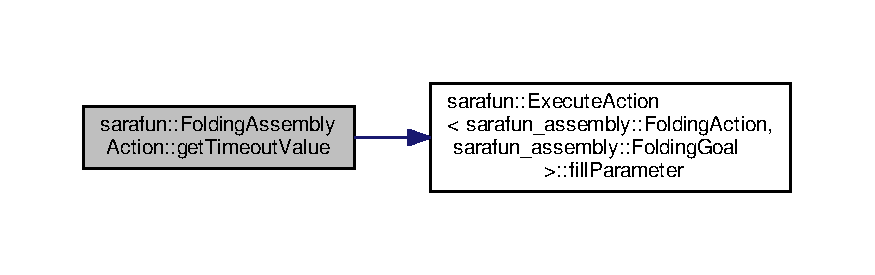
\includegraphics[width=350pt]{dd/df2/classsarafun_1_1FoldingAssemblyAction_a14174e375aa1b8d5b63159f275b7d971_a14174e375aa1b8d5b63159f275b7d971_cgraph}
\end{center}
\end{figure}




\subsection{Field Documentation}
\hypertarget{classsarafun_1_1FoldingAssemblyAction_a058ad644052e931e604053b6064f7576_a058ad644052e931e604053b6064f7576}{\index{sarafun\-::\-Folding\-Assembly\-Action@{sarafun\-::\-Folding\-Assembly\-Action}!bt\-\_\-name\-\_\-@{bt\-\_\-name\-\_\-}}
\index{bt\-\_\-name\-\_\-@{bt\-\_\-name\-\_\-}!sarafun::FoldingAssemblyAction@{sarafun\-::\-Folding\-Assembly\-Action}}
\subsubsection[{bt\-\_\-name\-\_\-}]{\setlength{\rightskip}{0pt plus 5cm}std\-::string sarafun\-::\-Folding\-Assembly\-Action\-::bt\-\_\-name\-\_\-\hspace{0.3cm}{\ttfamily [private]}}}\label{classsarafun_1_1FoldingAssemblyAction_a058ad644052e931e604053b6064f7576_a058ad644052e931e604053b6064f7576}


Definition at line 29 of file Folding\-Assembly\-Action.\-h.

\hypertarget{classsarafun_1_1FoldingAssemblyAction_a93ef41f7c8fe0fff59227e01deae7625_a93ef41f7c8fe0fff59227e01deae7625}{\index{sarafun\-::\-Folding\-Assembly\-Action@{sarafun\-::\-Folding\-Assembly\-Action}!node\-\_\-handle\-\_\-@{node\-\_\-handle\-\_\-}}
\index{node\-\_\-handle\-\_\-@{node\-\_\-handle\-\_\-}!sarafun::FoldingAssemblyAction@{sarafun\-::\-Folding\-Assembly\-Action}}
\subsubsection[{node\-\_\-handle\-\_\-}]{\setlength{\rightskip}{0pt plus 5cm}ros\-::\-Node\-Handle sarafun\-::\-Folding\-Assembly\-Action\-::node\-\_\-handle\-\_\-\hspace{0.3cm}{\ttfamily [private]}}}\label{classsarafun_1_1FoldingAssemblyAction_a93ef41f7c8fe0fff59227e01deae7625_a93ef41f7c8fe0fff59227e01deae7625}


Definition at line 27 of file Folding\-Assembly\-Action.\-h.



Referenced by Folding\-Assembly\-Action().

\hypertarget{classsarafun_1_1FoldingAssemblyAction_a80098bc35b0c446a61b0e84f4e97c8ab_a80098bc35b0c446a61b0e84f4e97c8ab}{\index{sarafun\-::\-Folding\-Assembly\-Action@{sarafun\-::\-Folding\-Assembly\-Action}!node\-\_\-name\-\_\-@{node\-\_\-name\-\_\-}}
\index{node\-\_\-name\-\_\-@{node\-\_\-name\-\_\-}!sarafun::FoldingAssemblyAction@{sarafun\-::\-Folding\-Assembly\-Action}}
\subsubsection[{node\-\_\-name\-\_\-}]{\setlength{\rightskip}{0pt plus 5cm}std\-::string sarafun\-::\-Folding\-Assembly\-Action\-::node\-\_\-name\-\_\-\hspace{0.3cm}{\ttfamily [private]}}}\label{classsarafun_1_1FoldingAssemblyAction_a80098bc35b0c446a61b0e84f4e97c8ab_a80098bc35b0c446a61b0e84f4e97c8ab}


Definition at line 28 of file Folding\-Assembly\-Action.\-h.



The documentation for this class was generated from the following files\-:\begin{DoxyCompactItemize}
\item 
Folding\-Assembly\-Action.\-h\item 
Folding\-Assembly\-Action.\-cpp\end{DoxyCompactItemize}

\hypertarget{classsarafun_1_1GrabObjectAction}{\section{sarafun\-:\-:Grab\-Object\-Action Class Reference}
\label{classsarafun_1_1GrabObjectAction}\index{sarafun\-::\-Grab\-Object\-Action@{sarafun\-::\-Grab\-Object\-Action}}
}


{\ttfamily \#include $<$Grab\-Object\-Action.\-h$>$}



Inheritance diagram for sarafun\-:\-:Grab\-Object\-Action\-:
\nopagebreak
\begin{figure}[H]
\begin{center}
\leavevmode
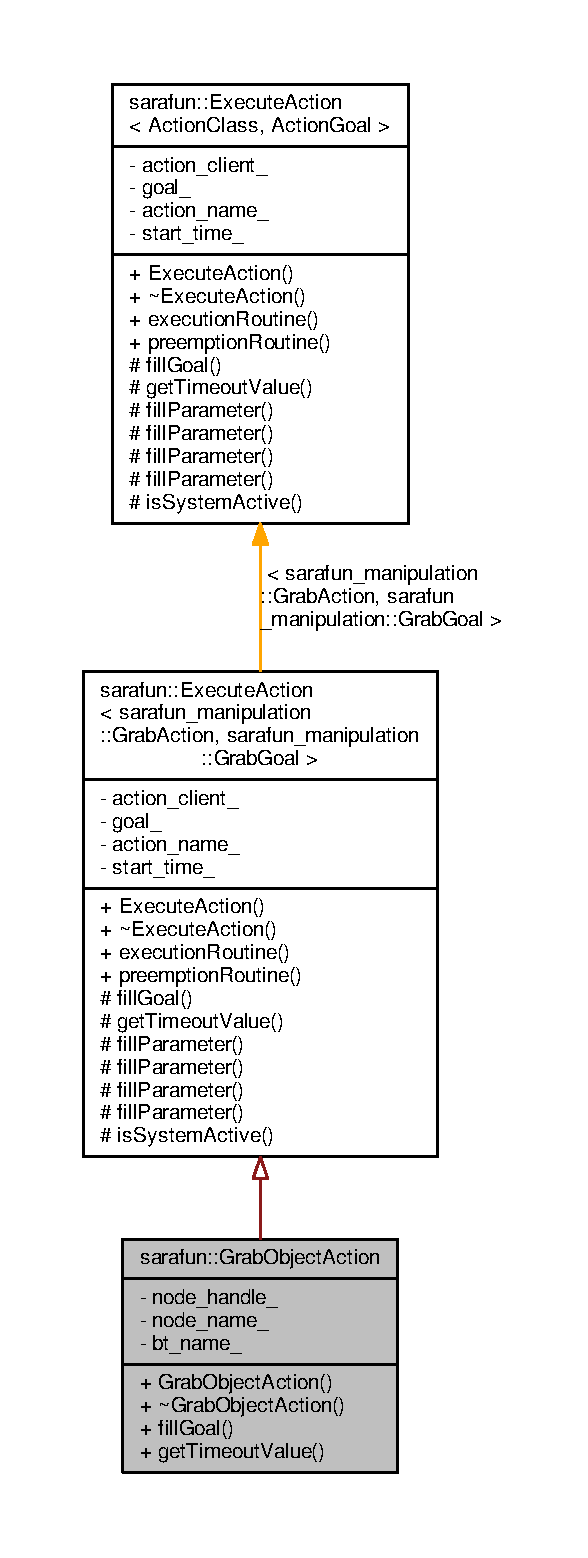
\includegraphics[height=550pt]{db/dc6/classsarafun_1_1GrabObjectAction__inherit__graph}
\end{center}
\end{figure}


Collaboration diagram for sarafun\-:\-:Grab\-Object\-Action\-:
\nopagebreak
\begin{figure}[H]
\begin{center}
\leavevmode
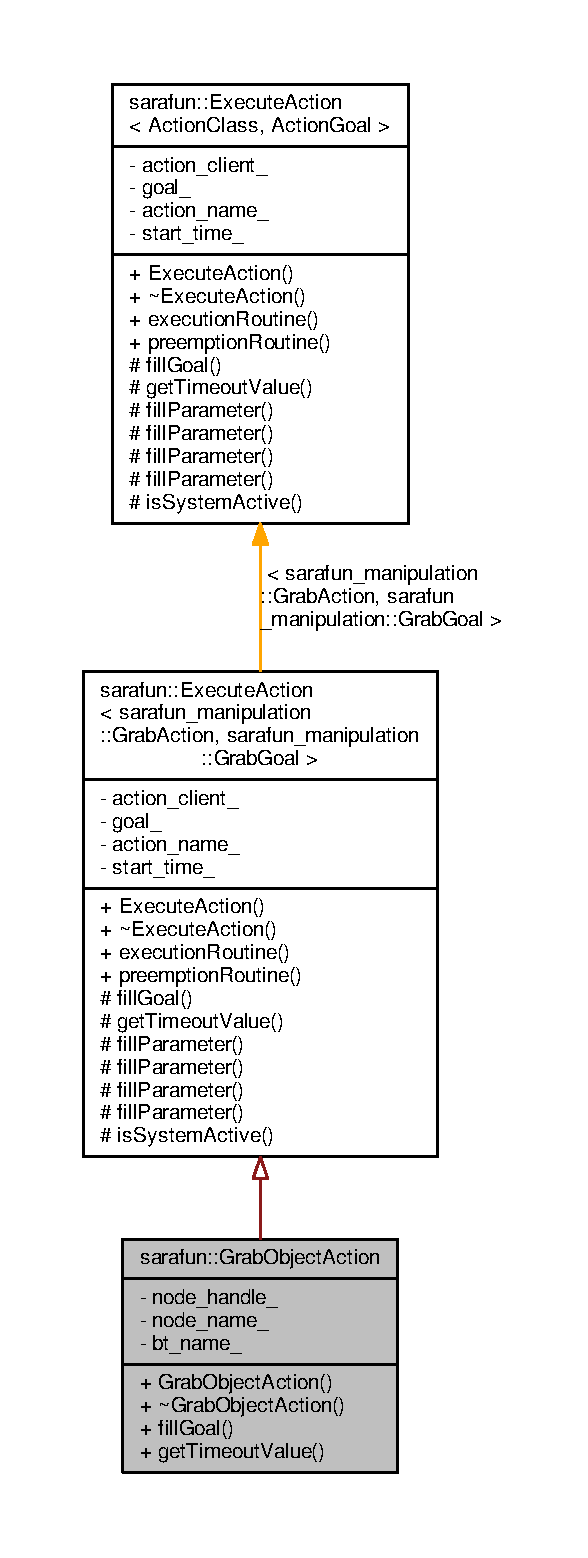
\includegraphics[height=550pt]{d7/d04/classsarafun_1_1GrabObjectAction__coll__graph}
\end{center}
\end{figure}
\subsection*{Public Member Functions}
\begin{DoxyCompactItemize}
\item 
\hyperlink{classsarafun_1_1GrabObjectAction_abca8f2d915cf1a8d507d04885b3e1df9_abca8f2d915cf1a8d507d04885b3e1df9}{Grab\-Object\-Action} (std\-::string node\-\_\-name, std\-::string action\-\_\-name, std\-::string bt\-\_\-name)
\item 
\hyperlink{classsarafun_1_1GrabObjectAction_a1b1ee63f9ba24332b2184b67021dbf0e_a1b1ee63f9ba24332b2184b67021dbf0e}{$\sim$\-Grab\-Object\-Action} ()
\item 
bool \hyperlink{classsarafun_1_1GrabObjectAction_a61fe8b0cb93dec244f10d6c5dbee913c_a61fe8b0cb93dec244f10d6c5dbee913c}{fill\-Goal} (sarafun\-\_\-manipulation\-::\-Grab\-Goal \&goal)
\item 
double \hyperlink{classsarafun_1_1GrabObjectAction_a6e2ee834fda8bd8d0dbdc101c8acdd9c_a6e2ee834fda8bd8d0dbdc101c8acdd9c}{get\-Timeout\-Value} ()
\end{DoxyCompactItemize}
\subsection*{Private Attributes}
\begin{DoxyCompactItemize}
\item 
ros\-::\-Node\-Handle \hyperlink{classsarafun_1_1GrabObjectAction_add955e0266ed5eaf3b6f7b3b3bccd4ae_add955e0266ed5eaf3b6f7b3b3bccd4ae}{node\-\_\-handle\-\_\-}
\item 
std\-::string \hyperlink{classsarafun_1_1GrabObjectAction_a586c34a94df1b7d435617d6b753d9e11_a586c34a94df1b7d435617d6b753d9e11}{node\-\_\-name\-\_\-}
\item 
std\-::string \hyperlink{classsarafun_1_1GrabObjectAction_a99b30dab79220943e417769f1a3d4f36_a99b30dab79220943e417769f1a3d4f36}{bt\-\_\-name\-\_\-}
\end{DoxyCompactItemize}
\subsection*{Additional Inherited Members}


\subsection{Detailed Description}


Definition at line 9 of file Grab\-Object\-Action.\-h.



\subsection{Constructor \& Destructor Documentation}
\hypertarget{classsarafun_1_1GrabObjectAction_abca8f2d915cf1a8d507d04885b3e1df9_abca8f2d915cf1a8d507d04885b3e1df9}{\index{sarafun\-::\-Grab\-Object\-Action@{sarafun\-::\-Grab\-Object\-Action}!Grab\-Object\-Action@{Grab\-Object\-Action}}
\index{Grab\-Object\-Action@{Grab\-Object\-Action}!sarafun::GrabObjectAction@{sarafun\-::\-Grab\-Object\-Action}}
\subsubsection[{Grab\-Object\-Action}]{\setlength{\rightskip}{0pt plus 5cm}sarafun\-::\-Grab\-Object\-Action\-::\-Grab\-Object\-Action (
\begin{DoxyParamCaption}
\item[{std\-::string}]{node\-\_\-name, }
\item[{std\-::string}]{action\-\_\-name, }
\item[{std\-::string}]{bt\-\_\-name}
\end{DoxyParamCaption}
)\hspace{0.3cm}{\ttfamily [inline]}}}\label{classsarafun_1_1GrabObjectAction_abca8f2d915cf1a8d507d04885b3e1df9_abca8f2d915cf1a8d507d04885b3e1df9}


Definition at line 12 of file Grab\-Object\-Action.\-h.



References node\-\_\-handle\-\_\-.

\hypertarget{classsarafun_1_1GrabObjectAction_a1b1ee63f9ba24332b2184b67021dbf0e_a1b1ee63f9ba24332b2184b67021dbf0e}{\index{sarafun\-::\-Grab\-Object\-Action@{sarafun\-::\-Grab\-Object\-Action}!$\sim$\-Grab\-Object\-Action@{$\sim$\-Grab\-Object\-Action}}
\index{$\sim$\-Grab\-Object\-Action@{$\sim$\-Grab\-Object\-Action}!sarafun::GrabObjectAction@{sarafun\-::\-Grab\-Object\-Action}}
\subsubsection[{$\sim$\-Grab\-Object\-Action}]{\setlength{\rightskip}{0pt plus 5cm}sarafun\-::\-Grab\-Object\-Action\-::$\sim$\-Grab\-Object\-Action (
\begin{DoxyParamCaption}
{}
\end{DoxyParamCaption}
)\hspace{0.3cm}{\ttfamily [inline]}}}\label{classsarafun_1_1GrabObjectAction_a1b1ee63f9ba24332b2184b67021dbf0e_a1b1ee63f9ba24332b2184b67021dbf0e}


Definition at line 22 of file Grab\-Object\-Action.\-h.



\subsection{Member Function Documentation}
\hypertarget{classsarafun_1_1GrabObjectAction_a61fe8b0cb93dec244f10d6c5dbee913c_a61fe8b0cb93dec244f10d6c5dbee913c}{\index{sarafun\-::\-Grab\-Object\-Action@{sarafun\-::\-Grab\-Object\-Action}!fill\-Goal@{fill\-Goal}}
\index{fill\-Goal@{fill\-Goal}!sarafun::GrabObjectAction@{sarafun\-::\-Grab\-Object\-Action}}
\subsubsection[{fill\-Goal}]{\setlength{\rightskip}{0pt plus 5cm}bool sarafun\-::\-Grab\-Object\-Action\-::fill\-Goal (
\begin{DoxyParamCaption}
\item[{sarafun\-\_\-manipulation\-::\-Grab\-Goal \&}]{goal}
\end{DoxyParamCaption}
)\hspace{0.3cm}{\ttfamily [virtual]}}}\label{classsarafun_1_1GrabObjectAction_a61fe8b0cb93dec244f10d6c5dbee913c_a61fe8b0cb93dec244f10d6c5dbee913c}
Fills in the goal for a particular action.


\begin{DoxyParams}{Parameters}
{\em goal} & The actionlib goal message of the externally implemented action. \\
\hline
\end{DoxyParams}
\begin{DoxyReturn}{Returns}
False in case of error, true otherwise. 
\end{DoxyReturn}


Implements \hyperlink{classsarafun_1_1ExecuteAction_a6dd9c0f013d15a17d7e7ce8dbe40a436_a6dd9c0f013d15a17d7e7ce8dbe40a436}{sarafun\-::\-Execute\-Action$<$ sarafun\-\_\-manipulation\-::\-Grab\-Action, sarafun\-\_\-manipulation\-::\-Grab\-Goal $>$}.



Definition at line 10 of file Grab\-Object\-Action.\-cpp.

\hypertarget{classsarafun_1_1GrabObjectAction_a6e2ee834fda8bd8d0dbdc101c8acdd9c_a6e2ee834fda8bd8d0dbdc101c8acdd9c}{\index{sarafun\-::\-Grab\-Object\-Action@{sarafun\-::\-Grab\-Object\-Action}!get\-Timeout\-Value@{get\-Timeout\-Value}}
\index{get\-Timeout\-Value@{get\-Timeout\-Value}!sarafun::GrabObjectAction@{sarafun\-::\-Grab\-Object\-Action}}
\subsubsection[{get\-Timeout\-Value}]{\setlength{\rightskip}{0pt plus 5cm}double sarafun\-::\-Grab\-Object\-Action\-::get\-Timeout\-Value (
\begin{DoxyParamCaption}
{}
\end{DoxyParamCaption}
)\hspace{0.3cm}{\ttfamily [virtual]}}}\label{classsarafun_1_1GrabObjectAction_a6e2ee834fda8bd8d0dbdc101c8acdd9c_a6e2ee834fda8bd8d0dbdc101c8acdd9c}
Provides the client with a timeout value for actionlib connections.

\begin{DoxyReturn}{Returns}
The timeout value (in seconds). 
\end{DoxyReturn}


Implements \hyperlink{classsarafun_1_1ExecuteAction_aba6cfa8a8ce19e735eb6394424df6d17_aba6cfa8a8ce19e735eb6394424df6d17}{sarafun\-::\-Execute\-Action$<$ sarafun\-\_\-manipulation\-::\-Grab\-Action, sarafun\-\_\-manipulation\-::\-Grab\-Goal $>$}.



Definition at line 4 of file Grab\-Object\-Action.\-cpp.



References sarafun\-::\-Execute\-Action$<$ sarafun\-\_\-manipulation\-::\-Grab\-Action, sarafun\-\_\-manipulation\-::\-Grab\-Goal $>$\-::fill\-Parameter().



Here is the call graph for this function\-:
\nopagebreak
\begin{figure}[H]
\begin{center}
\leavevmode
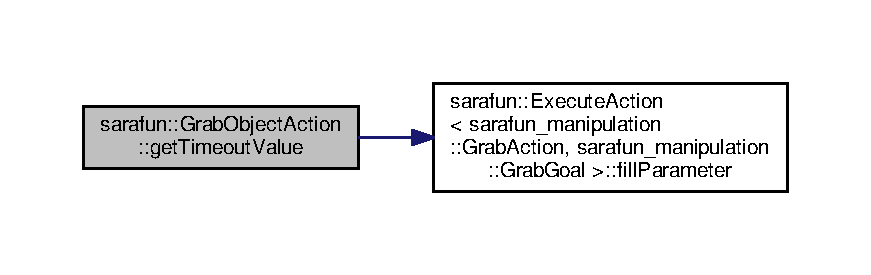
\includegraphics[width=350pt]{db/d0c/classsarafun_1_1GrabObjectAction_a6e2ee834fda8bd8d0dbdc101c8acdd9c_a6e2ee834fda8bd8d0dbdc101c8acdd9c_cgraph}
\end{center}
\end{figure}




\subsection{Field Documentation}
\hypertarget{classsarafun_1_1GrabObjectAction_a99b30dab79220943e417769f1a3d4f36_a99b30dab79220943e417769f1a3d4f36}{\index{sarafun\-::\-Grab\-Object\-Action@{sarafun\-::\-Grab\-Object\-Action}!bt\-\_\-name\-\_\-@{bt\-\_\-name\-\_\-}}
\index{bt\-\_\-name\-\_\-@{bt\-\_\-name\-\_\-}!sarafun::GrabObjectAction@{sarafun\-::\-Grab\-Object\-Action}}
\subsubsection[{bt\-\_\-name\-\_\-}]{\setlength{\rightskip}{0pt plus 5cm}std\-::string sarafun\-::\-Grab\-Object\-Action\-::bt\-\_\-name\-\_\-\hspace{0.3cm}{\ttfamily [private]}}}\label{classsarafun_1_1GrabObjectAction_a99b30dab79220943e417769f1a3d4f36_a99b30dab79220943e417769f1a3d4f36}


Definition at line 30 of file Grab\-Object\-Action.\-h.

\hypertarget{classsarafun_1_1GrabObjectAction_add955e0266ed5eaf3b6f7b3b3bccd4ae_add955e0266ed5eaf3b6f7b3b3bccd4ae}{\index{sarafun\-::\-Grab\-Object\-Action@{sarafun\-::\-Grab\-Object\-Action}!node\-\_\-handle\-\_\-@{node\-\_\-handle\-\_\-}}
\index{node\-\_\-handle\-\_\-@{node\-\_\-handle\-\_\-}!sarafun::GrabObjectAction@{sarafun\-::\-Grab\-Object\-Action}}
\subsubsection[{node\-\_\-handle\-\_\-}]{\setlength{\rightskip}{0pt plus 5cm}ros\-::\-Node\-Handle sarafun\-::\-Grab\-Object\-Action\-::node\-\_\-handle\-\_\-\hspace{0.3cm}{\ttfamily [private]}}}\label{classsarafun_1_1GrabObjectAction_add955e0266ed5eaf3b6f7b3b3bccd4ae_add955e0266ed5eaf3b6f7b3b3bccd4ae}


Definition at line 28 of file Grab\-Object\-Action.\-h.



Referenced by Grab\-Object\-Action().

\hypertarget{classsarafun_1_1GrabObjectAction_a586c34a94df1b7d435617d6b753d9e11_a586c34a94df1b7d435617d6b753d9e11}{\index{sarafun\-::\-Grab\-Object\-Action@{sarafun\-::\-Grab\-Object\-Action}!node\-\_\-name\-\_\-@{node\-\_\-name\-\_\-}}
\index{node\-\_\-name\-\_\-@{node\-\_\-name\-\_\-}!sarafun::GrabObjectAction@{sarafun\-::\-Grab\-Object\-Action}}
\subsubsection[{node\-\_\-name\-\_\-}]{\setlength{\rightskip}{0pt plus 5cm}std\-::string sarafun\-::\-Grab\-Object\-Action\-::node\-\_\-name\-\_\-\hspace{0.3cm}{\ttfamily [private]}}}\label{classsarafun_1_1GrabObjectAction_a586c34a94df1b7d435617d6b753d9e11_a586c34a94df1b7d435617d6b753d9e11}


Definition at line 29 of file Grab\-Object\-Action.\-h.



The documentation for this class was generated from the following files\-:\begin{DoxyCompactItemize}
\item 
Grab\-Object\-Action.\-h\item 
Grab\-Object\-Action.\-cpp\end{DoxyCompactItemize}

\hypertarget{classsarafun_1_1GraspAction}{\section{sarafun\-:\-:Grasp\-Action Class Reference}
\label{classsarafun_1_1GraspAction}\index{sarafun\-::\-Grasp\-Action@{sarafun\-::\-Grasp\-Action}}
}


{\ttfamily \#include $<$Grasp\-Action.\-h$>$}



Inheritance diagram for sarafun\-:\-:Grasp\-Action\-:\nopagebreak
\begin{figure}[H]
\begin{center}
\leavevmode
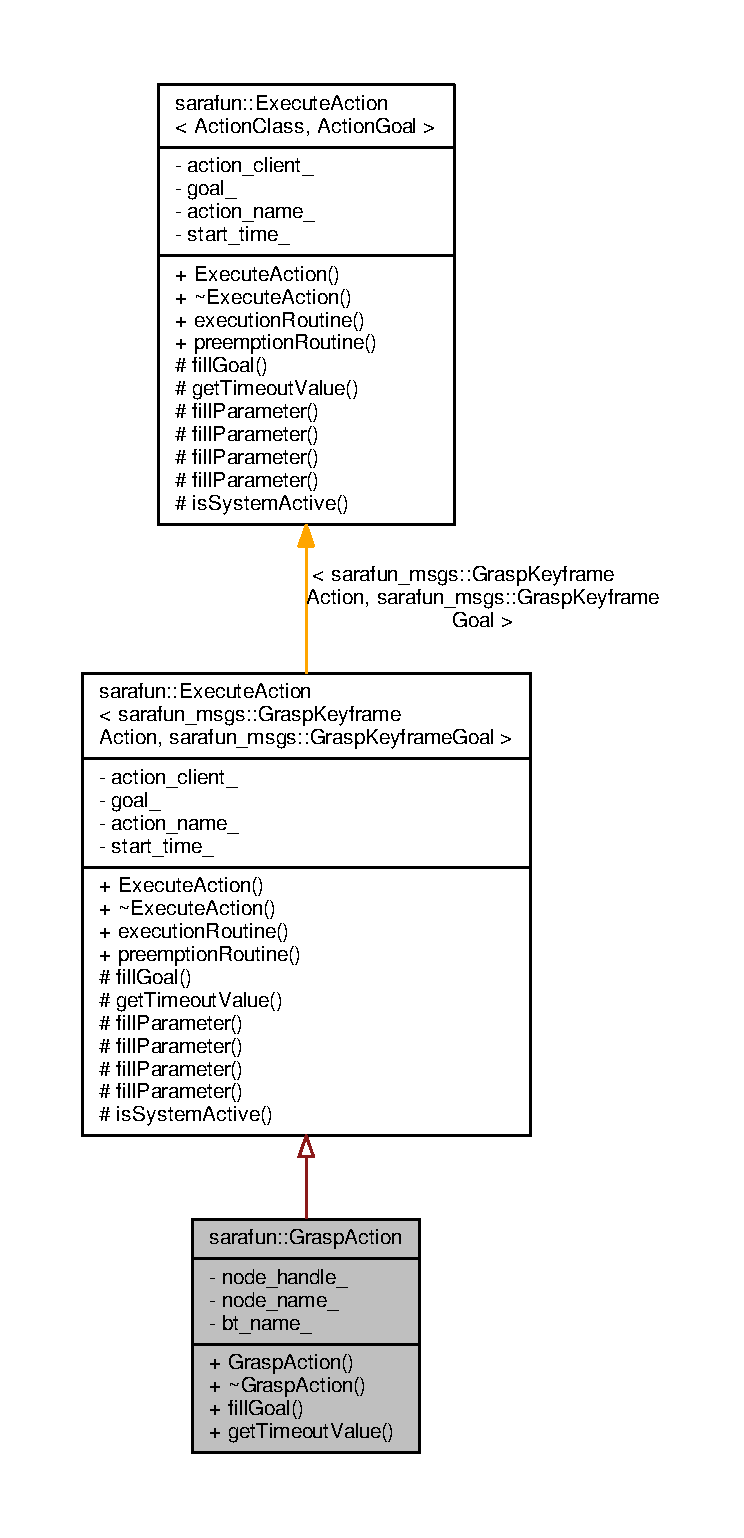
\includegraphics[height=550pt]{de/d55/classsarafun_1_1GraspAction__inherit__graph}
\end{center}
\end{figure}


Collaboration diagram for sarafun\-:\-:Grasp\-Action\-:\nopagebreak
\begin{figure}[H]
\begin{center}
\leavevmode
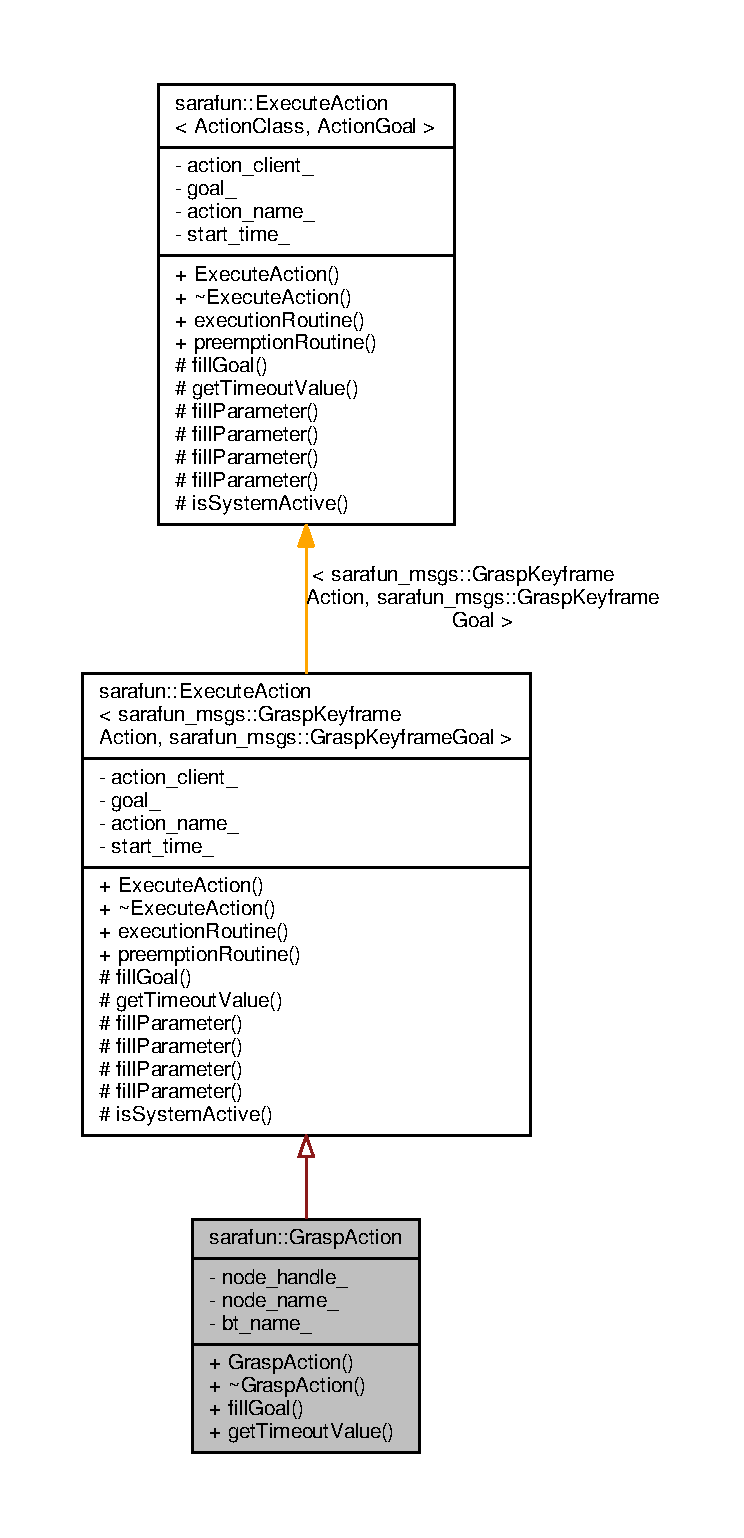
\includegraphics[height=550pt]{d0/dab/classsarafun_1_1GraspAction__coll__graph}
\end{center}
\end{figure}
\subsection*{Public Member Functions}
\begin{DoxyCompactItemize}
\item 
\hyperlink{classsarafun_1_1GraspAction_ae3eed6fe11388023bab8316803759ac5_ae3eed6fe11388023bab8316803759ac5}{Grasp\-Action} (std\-::string node\-\_\-name, std\-::string action\-\_\-name, std\-::string bt\-\_\-name)
\item 
\hyperlink{classsarafun_1_1GraspAction_aeb09ce6ab575e2653bfb88aa62b09361_aeb09ce6ab575e2653bfb88aa62b09361}{$\sim$\-Grasp\-Action} ()
\item 
bool \hyperlink{classsarafun_1_1GraspAction_a7418fe9de5024a8fbbfe8e5f5336d66f_a7418fe9de5024a8fbbfe8e5f5336d66f}{fill\-Goal} (sarafun\-\_\-msgs\-::\-Grasp\-Keyframe\-Goal \&goal)
\item 
double \hyperlink{classsarafun_1_1GraspAction_a406d5c86b5f788537c5af9d125724a55_a406d5c86b5f788537c5af9d125724a55}{get\-Timeout\-Value} ()
\end{DoxyCompactItemize}
\subsection*{Private Attributes}
\begin{DoxyCompactItemize}
\item 
ros\-::\-Node\-Handle \hyperlink{classsarafun_1_1GraspAction_a4b39e13eba27c71ee0d2cce0243b3e08_a4b39e13eba27c71ee0d2cce0243b3e08}{node\-\_\-handle\-\_\-}
\item 
std\-::string \hyperlink{classsarafun_1_1GraspAction_afd7e5985ad75e7b94ccd3190243d9df2_afd7e5985ad75e7b94ccd3190243d9df2}{node\-\_\-name\-\_\-}
\item 
std\-::string \hyperlink{classsarafun_1_1GraspAction_a3c06e926769370c2e80f864f8f36b958_a3c06e926769370c2e80f864f8f36b958}{bt\-\_\-name\-\_\-}
\end{DoxyCompactItemize}
\subsection*{Additional Inherited Members}


\subsection{Detailed Description}


Definition at line 9 of file Grasp\-Action.\-h.



\subsection{Constructor \& Destructor Documentation}
\hypertarget{classsarafun_1_1GraspAction_ae3eed6fe11388023bab8316803759ac5_ae3eed6fe11388023bab8316803759ac5}{\index{sarafun\-::\-Grasp\-Action@{sarafun\-::\-Grasp\-Action}!Grasp\-Action@{Grasp\-Action}}
\index{Grasp\-Action@{Grasp\-Action}!sarafun::GraspAction@{sarafun\-::\-Grasp\-Action}}
\subsubsection[{Grasp\-Action}]{\setlength{\rightskip}{0pt plus 5cm}sarafun\-::\-Grasp\-Action\-::\-Grasp\-Action (
\begin{DoxyParamCaption}
\item[{std\-::string}]{node\-\_\-name, }
\item[{std\-::string}]{action\-\_\-name, }
\item[{std\-::string}]{bt\-\_\-name}
\end{DoxyParamCaption}
)\hspace{0.3cm}{\ttfamily [inline]}}}\label{classsarafun_1_1GraspAction_ae3eed6fe11388023bab8316803759ac5_ae3eed6fe11388023bab8316803759ac5}


Definition at line 13 of file Grasp\-Action.\-h.



References node\-\_\-handle\-\_\-.

\hypertarget{classsarafun_1_1GraspAction_aeb09ce6ab575e2653bfb88aa62b09361_aeb09ce6ab575e2653bfb88aa62b09361}{\index{sarafun\-::\-Grasp\-Action@{sarafun\-::\-Grasp\-Action}!$\sim$\-Grasp\-Action@{$\sim$\-Grasp\-Action}}
\index{$\sim$\-Grasp\-Action@{$\sim$\-Grasp\-Action}!sarafun::GraspAction@{sarafun\-::\-Grasp\-Action}}
\subsubsection[{$\sim$\-Grasp\-Action}]{\setlength{\rightskip}{0pt plus 5cm}sarafun\-::\-Grasp\-Action\-::$\sim$\-Grasp\-Action (
\begin{DoxyParamCaption}
{}
\end{DoxyParamCaption}
)\hspace{0.3cm}{\ttfamily [inline]}}}\label{classsarafun_1_1GraspAction_aeb09ce6ab575e2653bfb88aa62b09361_aeb09ce6ab575e2653bfb88aa62b09361}


Definition at line 23 of file Grasp\-Action.\-h.



\subsection{Member Function Documentation}
\hypertarget{classsarafun_1_1GraspAction_a7418fe9de5024a8fbbfe8e5f5336d66f_a7418fe9de5024a8fbbfe8e5f5336d66f}{\index{sarafun\-::\-Grasp\-Action@{sarafun\-::\-Grasp\-Action}!fill\-Goal@{fill\-Goal}}
\index{fill\-Goal@{fill\-Goal}!sarafun::GraspAction@{sarafun\-::\-Grasp\-Action}}
\subsubsection[{fill\-Goal}]{\setlength{\rightskip}{0pt plus 5cm}bool sarafun\-::\-Grasp\-Action\-::fill\-Goal (
\begin{DoxyParamCaption}
\item[{sarafun\-\_\-msgs\-::\-Grasp\-Keyframe\-Goal \&}]{goal}
\end{DoxyParamCaption}
)\hspace{0.3cm}{\ttfamily [virtual]}}}\label{classsarafun_1_1GraspAction_a7418fe9de5024a8fbbfe8e5f5336d66f_a7418fe9de5024a8fbbfe8e5f5336d66f}
Fills in the goal for a particular action.


\begin{DoxyParams}{Parameters}
{\em goal} & The actionlib goal message of the externally implemented action. \\
\hline
\end{DoxyParams}
\begin{DoxyReturn}{Returns}
False in case of error, true otherwise. 
\end{DoxyReturn}


Implements \hyperlink{classsarafun_1_1ExecuteAction_a6dd9c0f013d15a17d7e7ce8dbe40a436_a6dd9c0f013d15a17d7e7ce8dbe40a436}{sarafun\-::\-Execute\-Action$<$ sarafun\-\_\-msgs\-::\-Grasp\-Keyframe\-Action, sarafun\-\_\-msgs\-::\-Grasp\-Keyframe\-Goal $>$}.



Definition at line 4 of file Grasp\-Action.\-cpp.

\hypertarget{classsarafun_1_1GraspAction_a406d5c86b5f788537c5af9d125724a55_a406d5c86b5f788537c5af9d125724a55}{\index{sarafun\-::\-Grasp\-Action@{sarafun\-::\-Grasp\-Action}!get\-Timeout\-Value@{get\-Timeout\-Value}}
\index{get\-Timeout\-Value@{get\-Timeout\-Value}!sarafun::GraspAction@{sarafun\-::\-Grasp\-Action}}
\subsubsection[{get\-Timeout\-Value}]{\setlength{\rightskip}{0pt plus 5cm}double sarafun\-::\-Grasp\-Action\-::get\-Timeout\-Value (
\begin{DoxyParamCaption}
{}
\end{DoxyParamCaption}
)\hspace{0.3cm}{\ttfamily [virtual]}}}\label{classsarafun_1_1GraspAction_a406d5c86b5f788537c5af9d125724a55_a406d5c86b5f788537c5af9d125724a55}
Provides the client with a timeout value for actionlib connections.

\begin{DoxyReturn}{Returns}
The timeout value (in seconds). 
\end{DoxyReturn}


Implements \hyperlink{classsarafun_1_1ExecuteAction_aba6cfa8a8ce19e735eb6394424df6d17_aba6cfa8a8ce19e735eb6394424df6d17}{sarafun\-::\-Execute\-Action$<$ sarafun\-\_\-msgs\-::\-Grasp\-Keyframe\-Action, sarafun\-\_\-msgs\-::\-Grasp\-Keyframe\-Goal $>$}.



Definition at line 8 of file Grasp\-Action.\-cpp.



References sarafun\-::\-Execute\-Action$<$ sarafun\-\_\-msgs\-::\-Grasp\-Keyframe\-Action, sarafun\-\_\-msgs\-::\-Grasp\-Keyframe\-Goal $>$\-::fill\-Parameter().



Here is the call graph for this function\-:\nopagebreak
\begin{figure}[H]
\begin{center}
\leavevmode
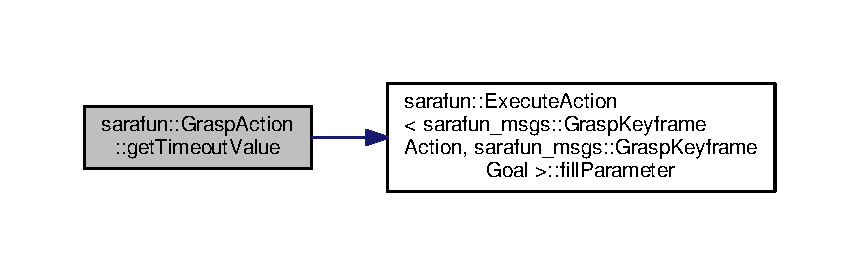
\includegraphics[width=350pt]{d0/d03/classsarafun_1_1GraspAction_a406d5c86b5f788537c5af9d125724a55_a406d5c86b5f788537c5af9d125724a55_cgraph}
\end{center}
\end{figure}




\subsection{Field Documentation}
\hypertarget{classsarafun_1_1GraspAction_a3c06e926769370c2e80f864f8f36b958_a3c06e926769370c2e80f864f8f36b958}{\index{sarafun\-::\-Grasp\-Action@{sarafun\-::\-Grasp\-Action}!bt\-\_\-name\-\_\-@{bt\-\_\-name\-\_\-}}
\index{bt\-\_\-name\-\_\-@{bt\-\_\-name\-\_\-}!sarafun::GraspAction@{sarafun\-::\-Grasp\-Action}}
\subsubsection[{bt\-\_\-name\-\_\-}]{\setlength{\rightskip}{0pt plus 5cm}std\-::string sarafun\-::\-Grasp\-Action\-::bt\-\_\-name\-\_\-\hspace{0.3cm}{\ttfamily [private]}}}\label{classsarafun_1_1GraspAction_a3c06e926769370c2e80f864f8f36b958_a3c06e926769370c2e80f864f8f36b958}


Definition at line 31 of file Grasp\-Action.\-h.

\hypertarget{classsarafun_1_1GraspAction_a4b39e13eba27c71ee0d2cce0243b3e08_a4b39e13eba27c71ee0d2cce0243b3e08}{\index{sarafun\-::\-Grasp\-Action@{sarafun\-::\-Grasp\-Action}!node\-\_\-handle\-\_\-@{node\-\_\-handle\-\_\-}}
\index{node\-\_\-handle\-\_\-@{node\-\_\-handle\-\_\-}!sarafun::GraspAction@{sarafun\-::\-Grasp\-Action}}
\subsubsection[{node\-\_\-handle\-\_\-}]{\setlength{\rightskip}{0pt plus 5cm}ros\-::\-Node\-Handle sarafun\-::\-Grasp\-Action\-::node\-\_\-handle\-\_\-\hspace{0.3cm}{\ttfamily [private]}}}\label{classsarafun_1_1GraspAction_a4b39e13eba27c71ee0d2cce0243b3e08_a4b39e13eba27c71ee0d2cce0243b3e08}


Definition at line 29 of file Grasp\-Action.\-h.



Referenced by Grasp\-Action().

\hypertarget{classsarafun_1_1GraspAction_afd7e5985ad75e7b94ccd3190243d9df2_afd7e5985ad75e7b94ccd3190243d9df2}{\index{sarafun\-::\-Grasp\-Action@{sarafun\-::\-Grasp\-Action}!node\-\_\-name\-\_\-@{node\-\_\-name\-\_\-}}
\index{node\-\_\-name\-\_\-@{node\-\_\-name\-\_\-}!sarafun::GraspAction@{sarafun\-::\-Grasp\-Action}}
\subsubsection[{node\-\_\-name\-\_\-}]{\setlength{\rightskip}{0pt plus 5cm}std\-::string sarafun\-::\-Grasp\-Action\-::node\-\_\-name\-\_\-\hspace{0.3cm}{\ttfamily [private]}}}\label{classsarafun_1_1GraspAction_afd7e5985ad75e7b94ccd3190243d9df2_afd7e5985ad75e7b94ccd3190243d9df2}


Definition at line 30 of file Grasp\-Action.\-h.



The documentation for this class was generated from the following files\-:\begin{DoxyCompactItemize}
\item 
Grasp\-Action.\-h\item 
Grasp\-Action.\-cpp\end{DoxyCompactItemize}

\hypertarget{structstd_1_1hash_3_01nlohmann_1_1json_01_4}{\section{std\-:\-:hash$<$ nlohmann\-:\-:json $>$ Struct Template Reference}
\label{structstd_1_1hash_3_01nlohmann_1_1json_01_4}\index{std\-::hash$<$ nlohmann\-::json $>$@{std\-::hash$<$ nlohmann\-::json $>$}}
}


hash value for J\-S\-O\-N objects  




{\ttfamily \#include $<$json.\-hpp$>$}

\subsection*{Public Member Functions}
\begin{DoxyCompactItemize}
\item 
std\-::size\-\_\-t \hyperlink{structstd_1_1hash_3_01nlohmann_1_1json_01_4_afd03f6ad53db22868ca4163a8200b2f9}{operator()} (const \hyperlink{namespacenlohmann_a9cc9a3033850a092f791d86854d117fc}{nlohmann\-::json} \&j) const 
\begin{DoxyCompactList}\small\item\em return a hash value for a J\-S\-O\-N object \end{DoxyCompactList}\item 
std\-::size\-\_\-t \hyperlink{structstd_1_1hash_3_01nlohmann_1_1json_01_4_afd03f6ad53db22868ca4163a8200b2f9}{operator()} (const \hyperlink{namespacenlohmann_a9cc9a3033850a092f791d86854d117fc}{nlohmann\-::json} \&j) const 
\begin{DoxyCompactList}\small\item\em return a hash value for a J\-S\-O\-N object \end{DoxyCompactList}\end{DoxyCompactItemize}


\subsection{Detailed Description}
\subsubsection*{template$<$$>$struct std\-::hash$<$ nlohmann\-::json $>$}

hash value for J\-S\-O\-N objects 

\subsection{Member Function Documentation}
\hypertarget{structstd_1_1hash_3_01nlohmann_1_1json_01_4_afd03f6ad53db22868ca4163a8200b2f9}{\index{std\-::hash$<$ nlohmann\-::json $>$@{std\-::hash$<$ nlohmann\-::json $>$}!operator()@{operator()}}
\index{operator()@{operator()}!std::hash< nlohmann::json >@{std\-::hash$<$ nlohmann\-::json $>$}}
\subsubsection[{operator()}]{\setlength{\rightskip}{0pt plus 5cm}std\-::size\-\_\-t std\-::hash$<$ {\bf nlohmann\-::json} $>$\-::operator() (
\begin{DoxyParamCaption}
\item[{const {\bf nlohmann\-::json} \&}]{j}
\end{DoxyParamCaption}
) const\hspace{0.3cm}{\ttfamily [inline]}}}\label{structstd_1_1hash_3_01nlohmann_1_1json_01_4_afd03f6ad53db22868ca4163a8200b2f9}


return a hash value for a J\-S\-O\-N object 

\begin{DoxySince}{Since}
version 1.\-0.\-0 
\end{DoxySince}
\hypertarget{structstd_1_1hash_3_01nlohmann_1_1json_01_4_afd03f6ad53db22868ca4163a8200b2f9}{\index{std\-::hash$<$ nlohmann\-::json $>$@{std\-::hash$<$ nlohmann\-::json $>$}!operator()@{operator()}}
\index{operator()@{operator()}!std::hash< nlohmann::json >@{std\-::hash$<$ nlohmann\-::json $>$}}
\subsubsection[{operator()}]{\setlength{\rightskip}{0pt plus 5cm}std\-::size\-\_\-t std\-::hash$<$ {\bf nlohmann\-::json} $>$\-::operator() (
\begin{DoxyParamCaption}
\item[{const {\bf nlohmann\-::json} \&}]{j}
\end{DoxyParamCaption}
) const\hspace{0.3cm}{\ttfamily [inline]}}}\label{structstd_1_1hash_3_01nlohmann_1_1json_01_4_afd03f6ad53db22868ca4163a8200b2f9}


return a hash value for a J\-S\-O\-N object 

\begin{DoxySince}{Since}
version 1.\-0.\-0 
\end{DoxySince}


The documentation for this struct was generated from the following file\-:\begin{DoxyCompactItemize}
\item 
sarafun\-\_\-tree/include/json/\hyperlink{sarafun__tree_2include_2json_2json_8hpp}{json.\-hpp}\end{DoxyCompactItemize}

\hypertarget{classsarafun_1_1InitialAction}{\section{sarafun\-:\-:Initial\-Action Class Reference}
\label{classsarafun_1_1InitialAction}\index{sarafun\-::\-Initial\-Action@{sarafun\-::\-Initial\-Action}}
}


{\ttfamily \#include $<$Initial\-Action.\-h$>$}



Inheritance diagram for sarafun\-:\-:Initial\-Action\-:\nopagebreak
\begin{figure}[H]
\begin{center}
\leavevmode
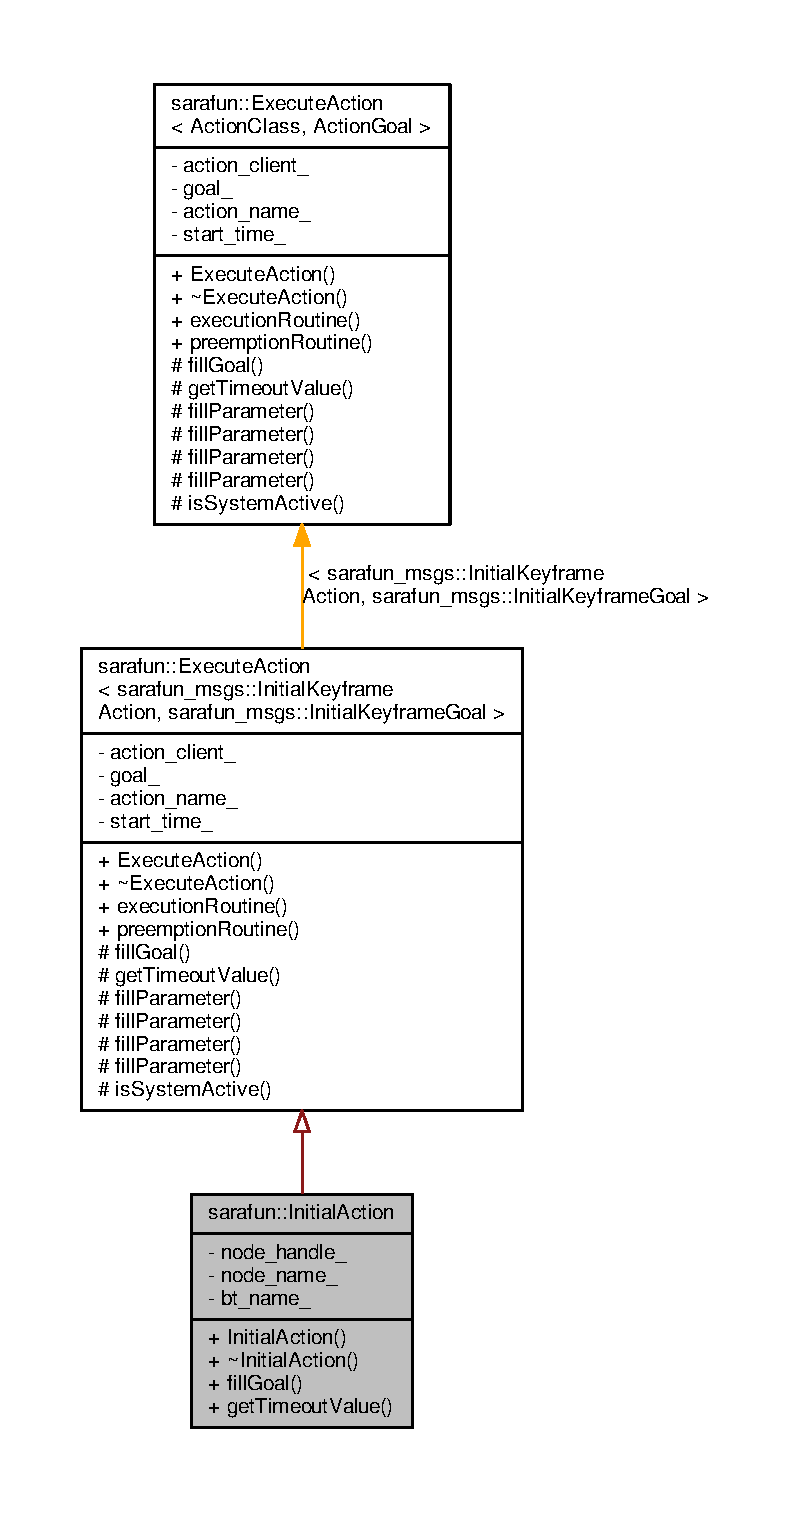
\includegraphics[height=550pt]{d2/dd7/classsarafun_1_1InitialAction__inherit__graph}
\end{center}
\end{figure}


Collaboration diagram for sarafun\-:\-:Initial\-Action\-:\nopagebreak
\begin{figure}[H]
\begin{center}
\leavevmode
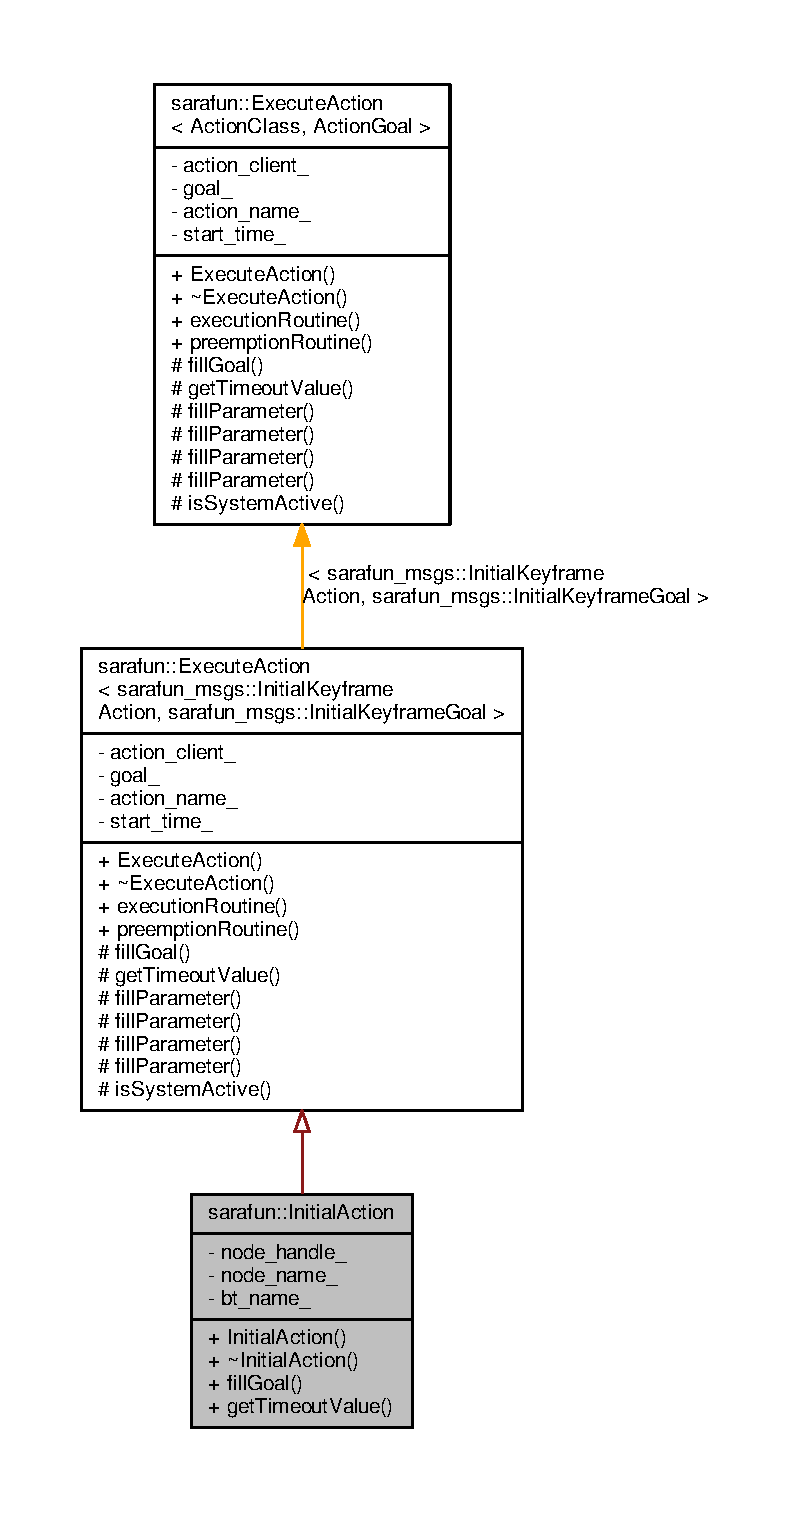
\includegraphics[height=550pt]{da/d64/classsarafun_1_1InitialAction__coll__graph}
\end{center}
\end{figure}
\subsection*{Public Member Functions}
\begin{DoxyCompactItemize}
\item 
\hyperlink{classsarafun_1_1InitialAction_afecd855fe18671ea36bdab881603e8bc_afecd855fe18671ea36bdab881603e8bc}{Initial\-Action} (std\-::string node\-\_\-name, std\-::string action\-\_\-name, std\-::string bt\-\_\-name)
\item 
\hyperlink{classsarafun_1_1InitialAction_af1f0a71513d093f5c2d7657b4b84661b_af1f0a71513d093f5c2d7657b4b84661b}{$\sim$\-Initial\-Action} ()
\item 
bool \hyperlink{classsarafun_1_1InitialAction_aac7f439c30455349e075e91542565a43_aac7f439c30455349e075e91542565a43}{fill\-Goal} (sarafun\-\_\-msgs\-::\-Initial\-Keyframe\-Goal \&goal)
\item 
double \hyperlink{classsarafun_1_1InitialAction_a1b58c06c32ec9f9d3e75c37de5e7d2c8_a1b58c06c32ec9f9d3e75c37de5e7d2c8}{get\-Timeout\-Value} ()
\end{DoxyCompactItemize}
\subsection*{Private Attributes}
\begin{DoxyCompactItemize}
\item 
ros\-::\-Node\-Handle \hyperlink{classsarafun_1_1InitialAction_ab28f63a6c2bfb376d0c52b619fb6b473_ab28f63a6c2bfb376d0c52b619fb6b473}{node\-\_\-handle\-\_\-}
\item 
std\-::string \hyperlink{classsarafun_1_1InitialAction_a985fe910cf04f8e6f918672175eb8ca6_a985fe910cf04f8e6f918672175eb8ca6}{node\-\_\-name\-\_\-}
\item 
std\-::string \hyperlink{classsarafun_1_1InitialAction_aaa1d120b5ff08ffaebe777d8f3793be3_aaa1d120b5ff08ffaebe777d8f3793be3}{bt\-\_\-name\-\_\-}
\end{DoxyCompactItemize}
\subsection*{Additional Inherited Members}


\subsection{Detailed Description}


Definition at line 9 of file Initial\-Action.\-h.



\subsection{Constructor \& Destructor Documentation}
\hypertarget{classsarafun_1_1InitialAction_afecd855fe18671ea36bdab881603e8bc_afecd855fe18671ea36bdab881603e8bc}{\index{sarafun\-::\-Initial\-Action@{sarafun\-::\-Initial\-Action}!Initial\-Action@{Initial\-Action}}
\index{Initial\-Action@{Initial\-Action}!sarafun::InitialAction@{sarafun\-::\-Initial\-Action}}
\subsubsection[{Initial\-Action}]{\setlength{\rightskip}{0pt plus 5cm}sarafun\-::\-Initial\-Action\-::\-Initial\-Action (
\begin{DoxyParamCaption}
\item[{std\-::string}]{node\-\_\-name, }
\item[{std\-::string}]{action\-\_\-name, }
\item[{std\-::string}]{bt\-\_\-name}
\end{DoxyParamCaption}
)\hspace{0.3cm}{\ttfamily [inline]}}}\label{classsarafun_1_1InitialAction_afecd855fe18671ea36bdab881603e8bc_afecd855fe18671ea36bdab881603e8bc}


Definition at line 13 of file Initial\-Action.\-h.



References node\-\_\-handle\-\_\-.

\hypertarget{classsarafun_1_1InitialAction_af1f0a71513d093f5c2d7657b4b84661b_af1f0a71513d093f5c2d7657b4b84661b}{\index{sarafun\-::\-Initial\-Action@{sarafun\-::\-Initial\-Action}!$\sim$\-Initial\-Action@{$\sim$\-Initial\-Action}}
\index{$\sim$\-Initial\-Action@{$\sim$\-Initial\-Action}!sarafun::InitialAction@{sarafun\-::\-Initial\-Action}}
\subsubsection[{$\sim$\-Initial\-Action}]{\setlength{\rightskip}{0pt plus 5cm}sarafun\-::\-Initial\-Action\-::$\sim$\-Initial\-Action (
\begin{DoxyParamCaption}
{}
\end{DoxyParamCaption}
)\hspace{0.3cm}{\ttfamily [inline]}}}\label{classsarafun_1_1InitialAction_af1f0a71513d093f5c2d7657b4b84661b_af1f0a71513d093f5c2d7657b4b84661b}


Definition at line 23 of file Initial\-Action.\-h.



\subsection{Member Function Documentation}
\hypertarget{classsarafun_1_1InitialAction_aac7f439c30455349e075e91542565a43_aac7f439c30455349e075e91542565a43}{\index{sarafun\-::\-Initial\-Action@{sarafun\-::\-Initial\-Action}!fill\-Goal@{fill\-Goal}}
\index{fill\-Goal@{fill\-Goal}!sarafun::InitialAction@{sarafun\-::\-Initial\-Action}}
\subsubsection[{fill\-Goal}]{\setlength{\rightskip}{0pt plus 5cm}bool sarafun\-::\-Initial\-Action\-::fill\-Goal (
\begin{DoxyParamCaption}
\item[{sarafun\-\_\-msgs\-::\-Initial\-Keyframe\-Goal \&}]{goal}
\end{DoxyParamCaption}
)\hspace{0.3cm}{\ttfamily [virtual]}}}\label{classsarafun_1_1InitialAction_aac7f439c30455349e075e91542565a43_aac7f439c30455349e075e91542565a43}
Fills in the goal for a particular action.


\begin{DoxyParams}{Parameters}
{\em goal} & The actionlib goal message of the externally implemented action. \\
\hline
\end{DoxyParams}
\begin{DoxyReturn}{Returns}
False in case of error, true otherwise. 
\end{DoxyReturn}


Implements \hyperlink{classsarafun_1_1ExecuteAction_a6dd9c0f013d15a17d7e7ce8dbe40a436_a6dd9c0f013d15a17d7e7ce8dbe40a436}{sarafun\-::\-Execute\-Action$<$ sarafun\-\_\-msgs\-::\-Initial\-Keyframe\-Action, sarafun\-\_\-msgs\-::\-Initial\-Keyframe\-Goal $>$}.



Definition at line 4 of file Initial\-Action.\-cpp.



References sarafun\-::\-Execute\-Action$<$ sarafun\-\_\-msgs\-::\-Initial\-Keyframe\-Action, sarafun\-\_\-msgs\-::\-Initial\-Keyframe\-Goal $>$\-::fill\-Parameter().



Here is the call graph for this function\-:\nopagebreak
\begin{figure}[H]
\begin{center}
\leavevmode
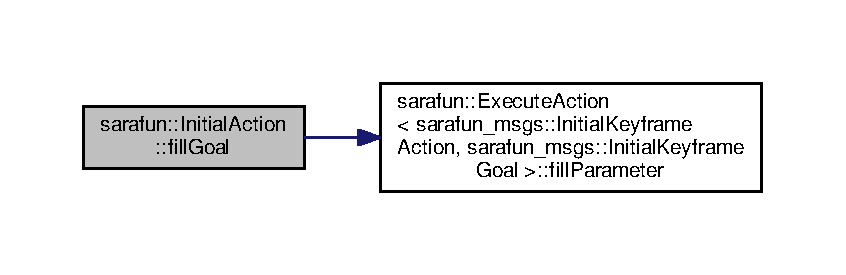
\includegraphics[width=350pt]{d6/d64/classsarafun_1_1InitialAction_aac7f439c30455349e075e91542565a43_aac7f439c30455349e075e91542565a43_cgraph}
\end{center}
\end{figure}


\hypertarget{classsarafun_1_1InitialAction_a1b58c06c32ec9f9d3e75c37de5e7d2c8_a1b58c06c32ec9f9d3e75c37de5e7d2c8}{\index{sarafun\-::\-Initial\-Action@{sarafun\-::\-Initial\-Action}!get\-Timeout\-Value@{get\-Timeout\-Value}}
\index{get\-Timeout\-Value@{get\-Timeout\-Value}!sarafun::InitialAction@{sarafun\-::\-Initial\-Action}}
\subsubsection[{get\-Timeout\-Value}]{\setlength{\rightskip}{0pt plus 5cm}double sarafun\-::\-Initial\-Action\-::get\-Timeout\-Value (
\begin{DoxyParamCaption}
{}
\end{DoxyParamCaption}
)\hspace{0.3cm}{\ttfamily [virtual]}}}\label{classsarafun_1_1InitialAction_a1b58c06c32ec9f9d3e75c37de5e7d2c8_a1b58c06c32ec9f9d3e75c37de5e7d2c8}
Provides the client with a timeout value for actionlib connections.

\begin{DoxyReturn}{Returns}
The timeout value (in seconds). 
\end{DoxyReturn}


Implements \hyperlink{classsarafun_1_1ExecuteAction_aba6cfa8a8ce19e735eb6394424df6d17_aba6cfa8a8ce19e735eb6394424df6d17}{sarafun\-::\-Execute\-Action$<$ sarafun\-\_\-msgs\-::\-Initial\-Keyframe\-Action, sarafun\-\_\-msgs\-::\-Initial\-Keyframe\-Goal $>$}.



Definition at line 13 of file Initial\-Action.\-cpp.



References sarafun\-::\-Execute\-Action$<$ sarafun\-\_\-msgs\-::\-Initial\-Keyframe\-Action, sarafun\-\_\-msgs\-::\-Initial\-Keyframe\-Goal $>$\-::fill\-Parameter().



Here is the call graph for this function\-:\nopagebreak
\begin{figure}[H]
\begin{center}
\leavevmode
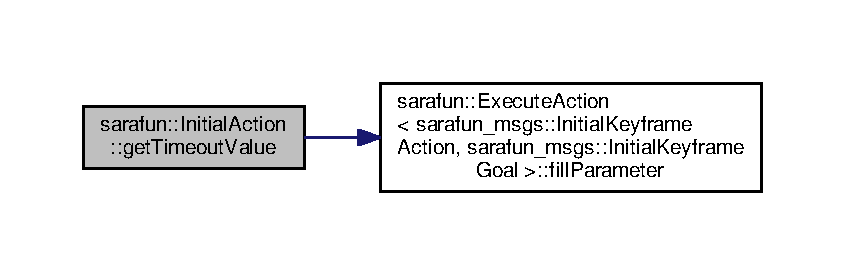
\includegraphics[width=350pt]{d6/d64/classsarafun_1_1InitialAction_a1b58c06c32ec9f9d3e75c37de5e7d2c8_a1b58c06c32ec9f9d3e75c37de5e7d2c8_cgraph}
\end{center}
\end{figure}




\subsection{Field Documentation}
\hypertarget{classsarafun_1_1InitialAction_aaa1d120b5ff08ffaebe777d8f3793be3_aaa1d120b5ff08ffaebe777d8f3793be3}{\index{sarafun\-::\-Initial\-Action@{sarafun\-::\-Initial\-Action}!bt\-\_\-name\-\_\-@{bt\-\_\-name\-\_\-}}
\index{bt\-\_\-name\-\_\-@{bt\-\_\-name\-\_\-}!sarafun::InitialAction@{sarafun\-::\-Initial\-Action}}
\subsubsection[{bt\-\_\-name\-\_\-}]{\setlength{\rightskip}{0pt plus 5cm}std\-::string sarafun\-::\-Initial\-Action\-::bt\-\_\-name\-\_\-\hspace{0.3cm}{\ttfamily [private]}}}\label{classsarafun_1_1InitialAction_aaa1d120b5ff08ffaebe777d8f3793be3_aaa1d120b5ff08ffaebe777d8f3793be3}


Definition at line 31 of file Initial\-Action.\-h.

\hypertarget{classsarafun_1_1InitialAction_ab28f63a6c2bfb376d0c52b619fb6b473_ab28f63a6c2bfb376d0c52b619fb6b473}{\index{sarafun\-::\-Initial\-Action@{sarafun\-::\-Initial\-Action}!node\-\_\-handle\-\_\-@{node\-\_\-handle\-\_\-}}
\index{node\-\_\-handle\-\_\-@{node\-\_\-handle\-\_\-}!sarafun::InitialAction@{sarafun\-::\-Initial\-Action}}
\subsubsection[{node\-\_\-handle\-\_\-}]{\setlength{\rightskip}{0pt plus 5cm}ros\-::\-Node\-Handle sarafun\-::\-Initial\-Action\-::node\-\_\-handle\-\_\-\hspace{0.3cm}{\ttfamily [private]}}}\label{classsarafun_1_1InitialAction_ab28f63a6c2bfb376d0c52b619fb6b473_ab28f63a6c2bfb376d0c52b619fb6b473}


Definition at line 29 of file Initial\-Action.\-h.



Referenced by Initial\-Action().

\hypertarget{classsarafun_1_1InitialAction_a985fe910cf04f8e6f918672175eb8ca6_a985fe910cf04f8e6f918672175eb8ca6}{\index{sarafun\-::\-Initial\-Action@{sarafun\-::\-Initial\-Action}!node\-\_\-name\-\_\-@{node\-\_\-name\-\_\-}}
\index{node\-\_\-name\-\_\-@{node\-\_\-name\-\_\-}!sarafun::InitialAction@{sarafun\-::\-Initial\-Action}}
\subsubsection[{node\-\_\-name\-\_\-}]{\setlength{\rightskip}{0pt plus 5cm}std\-::string sarafun\-::\-Initial\-Action\-::node\-\_\-name\-\_\-\hspace{0.3cm}{\ttfamily [private]}}}\label{classsarafun_1_1InitialAction_a985fe910cf04f8e6f918672175eb8ca6_a985fe910cf04f8e6f918672175eb8ca6}


Definition at line 30 of file Initial\-Action.\-h.



The documentation for this class was generated from the following files\-:\begin{DoxyCompactItemize}
\item 
Initial\-Action.\-h\item 
Initial\-Action.\-cpp\end{DoxyCompactItemize}

\hypertarget{classsarafun_1_1InsertionWithDeformationAction}{\section{sarafun\-:\-:Insertion\-With\-Deformation\-Action Class Reference}
\label{classsarafun_1_1InsertionWithDeformationAction}\index{sarafun\-::\-Insertion\-With\-Deformation\-Action@{sarafun\-::\-Insertion\-With\-Deformation\-Action}}
}


{\ttfamily \#include $<$Insertion\-With\-Deformation\-Action.\-h$>$}



Inheritance diagram for sarafun\-:\-:Insertion\-With\-Deformation\-Action\-:
\nopagebreak
\begin{figure}[H]
\begin{center}
\leavevmode
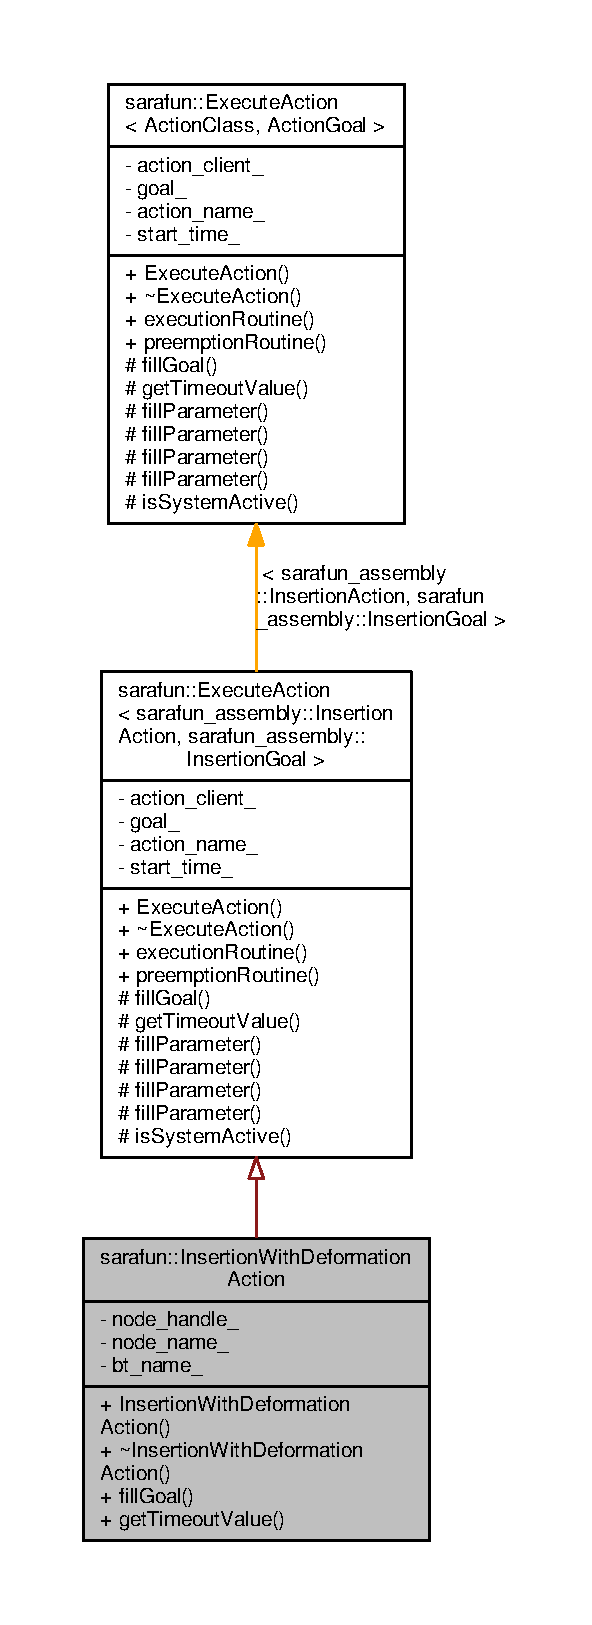
\includegraphics[height=550pt]{de/dd8/classsarafun_1_1InsertionWithDeformationAction__inherit__graph}
\end{center}
\end{figure}


Collaboration diagram for sarafun\-:\-:Insertion\-With\-Deformation\-Action\-:
\nopagebreak
\begin{figure}[H]
\begin{center}
\leavevmode
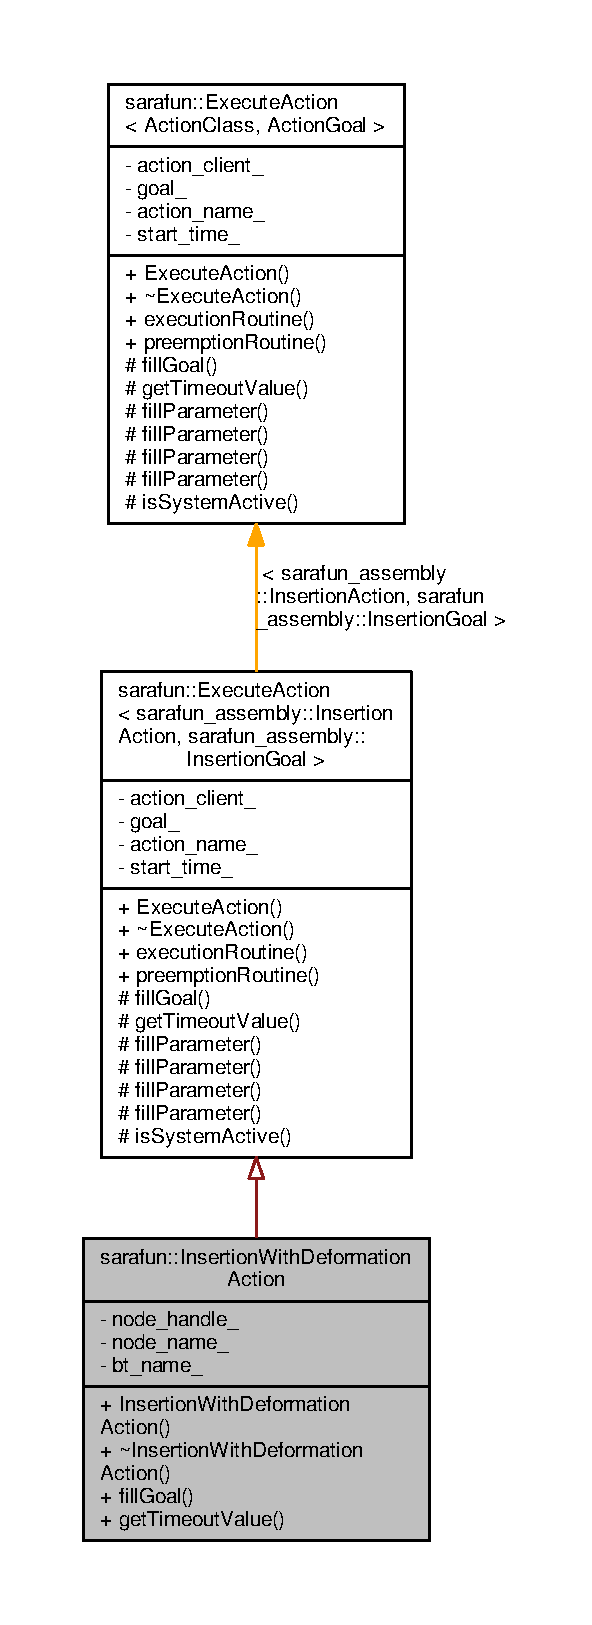
\includegraphics[height=550pt]{da/dd6/classsarafun_1_1InsertionWithDeformationAction__coll__graph}
\end{center}
\end{figure}
\subsection*{Public Member Functions}
\begin{DoxyCompactItemize}
\item 
\hyperlink{classsarafun_1_1InsertionWithDeformationAction_a2b851f2604c6a10f32b1d4b51bfae6a8_a2b851f2604c6a10f32b1d4b51bfae6a8}{Insertion\-With\-Deformation\-Action} (std\-::string node\-\_\-name, std\-::string action\-\_\-name, std\-::string bt\-\_\-name)
\item 
\hyperlink{classsarafun_1_1InsertionWithDeformationAction_a9b8740951e51538bf47d6534b8b4fe36_a9b8740951e51538bf47d6534b8b4fe36}{$\sim$\-Insertion\-With\-Deformation\-Action} ()
\item 
bool \hyperlink{classsarafun_1_1InsertionWithDeformationAction_a32d695dfcd626c5a7ca0fa987c245083_a32d695dfcd626c5a7ca0fa987c245083}{fill\-Goal} (sarafun\-\_\-assembly\-::\-Insertion\-Goal \&goal)
\item 
double \hyperlink{classsarafun_1_1InsertionWithDeformationAction_a8d77b104fb2396000b273cb6754ff879_a8d77b104fb2396000b273cb6754ff879}{get\-Timeout\-Value} ()
\end{DoxyCompactItemize}
\subsection*{Private Attributes}
\begin{DoxyCompactItemize}
\item 
ros\-::\-Node\-Handle \hyperlink{classsarafun_1_1InsertionWithDeformationAction_a97fcbe6b19d7f2185e19f5e8397b2307_a97fcbe6b19d7f2185e19f5e8397b2307}{node\-\_\-handle\-\_\-}
\item 
std\-::string \hyperlink{classsarafun_1_1InsertionWithDeformationAction_a493a532429347d18fa4d525d982c0204_a493a532429347d18fa4d525d982c0204}{node\-\_\-name\-\_\-}
\item 
std\-::string \hyperlink{classsarafun_1_1InsertionWithDeformationAction_aa5a6397046e4d8ac145d2961d04fc27c_aa5a6397046e4d8ac145d2961d04fc27c}{bt\-\_\-name\-\_\-}
\end{DoxyCompactItemize}
\subsection*{Additional Inherited Members}


\subsection{Detailed Description}


Definition at line 9 of file Insertion\-With\-Deformation\-Action.\-h.



\subsection{Constructor \& Destructor Documentation}
\hypertarget{classsarafun_1_1InsertionWithDeformationAction_a2b851f2604c6a10f32b1d4b51bfae6a8_a2b851f2604c6a10f32b1d4b51bfae6a8}{\index{sarafun\-::\-Insertion\-With\-Deformation\-Action@{sarafun\-::\-Insertion\-With\-Deformation\-Action}!Insertion\-With\-Deformation\-Action@{Insertion\-With\-Deformation\-Action}}
\index{Insertion\-With\-Deformation\-Action@{Insertion\-With\-Deformation\-Action}!sarafun::InsertionWithDeformationAction@{sarafun\-::\-Insertion\-With\-Deformation\-Action}}
\subsubsection[{Insertion\-With\-Deformation\-Action}]{\setlength{\rightskip}{0pt plus 5cm}sarafun\-::\-Insertion\-With\-Deformation\-Action\-::\-Insertion\-With\-Deformation\-Action (
\begin{DoxyParamCaption}
\item[{std\-::string}]{node\-\_\-name, }
\item[{std\-::string}]{action\-\_\-name, }
\item[{std\-::string}]{bt\-\_\-name}
\end{DoxyParamCaption}
)\hspace{0.3cm}{\ttfamily [inline]}}}\label{classsarafun_1_1InsertionWithDeformationAction_a2b851f2604c6a10f32b1d4b51bfae6a8_a2b851f2604c6a10f32b1d4b51bfae6a8}


Definition at line 13 of file Insertion\-With\-Deformation\-Action.\-h.



References node\-\_\-handle\-\_\-.

\hypertarget{classsarafun_1_1InsertionWithDeformationAction_a9b8740951e51538bf47d6534b8b4fe36_a9b8740951e51538bf47d6534b8b4fe36}{\index{sarafun\-::\-Insertion\-With\-Deformation\-Action@{sarafun\-::\-Insertion\-With\-Deformation\-Action}!$\sim$\-Insertion\-With\-Deformation\-Action@{$\sim$\-Insertion\-With\-Deformation\-Action}}
\index{$\sim$\-Insertion\-With\-Deformation\-Action@{$\sim$\-Insertion\-With\-Deformation\-Action}!sarafun::InsertionWithDeformationAction@{sarafun\-::\-Insertion\-With\-Deformation\-Action}}
\subsubsection[{$\sim$\-Insertion\-With\-Deformation\-Action}]{\setlength{\rightskip}{0pt plus 5cm}sarafun\-::\-Insertion\-With\-Deformation\-Action\-::$\sim$\-Insertion\-With\-Deformation\-Action (
\begin{DoxyParamCaption}
{}
\end{DoxyParamCaption}
)\hspace{0.3cm}{\ttfamily [inline]}}}\label{classsarafun_1_1InsertionWithDeformationAction_a9b8740951e51538bf47d6534b8b4fe36_a9b8740951e51538bf47d6534b8b4fe36}


Definition at line 23 of file Insertion\-With\-Deformation\-Action.\-h.



\subsection{Member Function Documentation}
\hypertarget{classsarafun_1_1InsertionWithDeformationAction_a32d695dfcd626c5a7ca0fa987c245083_a32d695dfcd626c5a7ca0fa987c245083}{\index{sarafun\-::\-Insertion\-With\-Deformation\-Action@{sarafun\-::\-Insertion\-With\-Deformation\-Action}!fill\-Goal@{fill\-Goal}}
\index{fill\-Goal@{fill\-Goal}!sarafun::InsertionWithDeformationAction@{sarafun\-::\-Insertion\-With\-Deformation\-Action}}
\subsubsection[{fill\-Goal}]{\setlength{\rightskip}{0pt plus 5cm}bool sarafun\-::\-Insertion\-With\-Deformation\-Action\-::fill\-Goal (
\begin{DoxyParamCaption}
\item[{sarafun\-\_\-assembly\-::\-Insertion\-Goal \&}]{goal}
\end{DoxyParamCaption}
)\hspace{0.3cm}{\ttfamily [virtual]}}}\label{classsarafun_1_1InsertionWithDeformationAction_a32d695dfcd626c5a7ca0fa987c245083_a32d695dfcd626c5a7ca0fa987c245083}
Fills in the goal for a particular action.


\begin{DoxyParams}{Parameters}
{\em goal} & The actionlib goal message of the externally implemented action. \\
\hline
\end{DoxyParams}
\begin{DoxyReturn}{Returns}
False in case of error, true otherwise. 
\end{DoxyReturn}


Implements \hyperlink{classsarafun_1_1ExecuteAction_a6dd9c0f013d15a17d7e7ce8dbe40a436_a6dd9c0f013d15a17d7e7ce8dbe40a436}{sarafun\-::\-Execute\-Action$<$ sarafun\-\_\-assembly\-::\-Insertion\-Action, sarafun\-\_\-assembly\-::\-Insertion\-Goal $>$}.



Definition at line 11 of file Insertion\-With\-Deformation\-Action.\-cpp.

\hypertarget{classsarafun_1_1InsertionWithDeformationAction_a8d77b104fb2396000b273cb6754ff879_a8d77b104fb2396000b273cb6754ff879}{\index{sarafun\-::\-Insertion\-With\-Deformation\-Action@{sarafun\-::\-Insertion\-With\-Deformation\-Action}!get\-Timeout\-Value@{get\-Timeout\-Value}}
\index{get\-Timeout\-Value@{get\-Timeout\-Value}!sarafun::InsertionWithDeformationAction@{sarafun\-::\-Insertion\-With\-Deformation\-Action}}
\subsubsection[{get\-Timeout\-Value}]{\setlength{\rightskip}{0pt plus 5cm}double sarafun\-::\-Insertion\-With\-Deformation\-Action\-::get\-Timeout\-Value (
\begin{DoxyParamCaption}
{}
\end{DoxyParamCaption}
)\hspace{0.3cm}{\ttfamily [virtual]}}}\label{classsarafun_1_1InsertionWithDeformationAction_a8d77b104fb2396000b273cb6754ff879_a8d77b104fb2396000b273cb6754ff879}
Provides the client with a timeout value for actionlib connections.

\begin{DoxyReturn}{Returns}
The timeout value (in seconds). 
\end{DoxyReturn}


Implements \hyperlink{classsarafun_1_1ExecuteAction_aba6cfa8a8ce19e735eb6394424df6d17_aba6cfa8a8ce19e735eb6394424df6d17}{sarafun\-::\-Execute\-Action$<$ sarafun\-\_\-assembly\-::\-Insertion\-Action, sarafun\-\_\-assembly\-::\-Insertion\-Goal $>$}.



Definition at line 4 of file Insertion\-With\-Deformation\-Action.\-cpp.



References sarafun\-::\-Execute\-Action$<$ sarafun\-\_\-assembly\-::\-Insertion\-Action, sarafun\-\_\-assembly\-::\-Insertion\-Goal $>$\-::fill\-Parameter().



Here is the call graph for this function\-:
\nopagebreak
\begin{figure}[H]
\begin{center}
\leavevmode
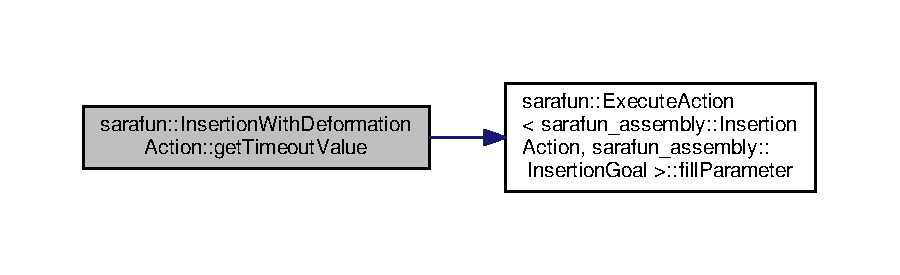
\includegraphics[width=350pt]{d8/db8/classsarafun_1_1InsertionWithDeformationAction_a8d77b104fb2396000b273cb6754ff879_a8d77b104fb2396000b273cb6754ff879_cgraph}
\end{center}
\end{figure}




\subsection{Field Documentation}
\hypertarget{classsarafun_1_1InsertionWithDeformationAction_aa5a6397046e4d8ac145d2961d04fc27c_aa5a6397046e4d8ac145d2961d04fc27c}{\index{sarafun\-::\-Insertion\-With\-Deformation\-Action@{sarafun\-::\-Insertion\-With\-Deformation\-Action}!bt\-\_\-name\-\_\-@{bt\-\_\-name\-\_\-}}
\index{bt\-\_\-name\-\_\-@{bt\-\_\-name\-\_\-}!sarafun::InsertionWithDeformationAction@{sarafun\-::\-Insertion\-With\-Deformation\-Action}}
\subsubsection[{bt\-\_\-name\-\_\-}]{\setlength{\rightskip}{0pt plus 5cm}std\-::string sarafun\-::\-Insertion\-With\-Deformation\-Action\-::bt\-\_\-name\-\_\-\hspace{0.3cm}{\ttfamily [private]}}}\label{classsarafun_1_1InsertionWithDeformationAction_aa5a6397046e4d8ac145d2961d04fc27c_aa5a6397046e4d8ac145d2961d04fc27c}


Definition at line 31 of file Insertion\-With\-Deformation\-Action.\-h.

\hypertarget{classsarafun_1_1InsertionWithDeformationAction_a97fcbe6b19d7f2185e19f5e8397b2307_a97fcbe6b19d7f2185e19f5e8397b2307}{\index{sarafun\-::\-Insertion\-With\-Deformation\-Action@{sarafun\-::\-Insertion\-With\-Deformation\-Action}!node\-\_\-handle\-\_\-@{node\-\_\-handle\-\_\-}}
\index{node\-\_\-handle\-\_\-@{node\-\_\-handle\-\_\-}!sarafun::InsertionWithDeformationAction@{sarafun\-::\-Insertion\-With\-Deformation\-Action}}
\subsubsection[{node\-\_\-handle\-\_\-}]{\setlength{\rightskip}{0pt plus 5cm}ros\-::\-Node\-Handle sarafun\-::\-Insertion\-With\-Deformation\-Action\-::node\-\_\-handle\-\_\-\hspace{0.3cm}{\ttfamily [private]}}}\label{classsarafun_1_1InsertionWithDeformationAction_a97fcbe6b19d7f2185e19f5e8397b2307_a97fcbe6b19d7f2185e19f5e8397b2307}


Definition at line 29 of file Insertion\-With\-Deformation\-Action.\-h.



Referenced by Insertion\-With\-Deformation\-Action().

\hypertarget{classsarafun_1_1InsertionWithDeformationAction_a493a532429347d18fa4d525d982c0204_a493a532429347d18fa4d525d982c0204}{\index{sarafun\-::\-Insertion\-With\-Deformation\-Action@{sarafun\-::\-Insertion\-With\-Deformation\-Action}!node\-\_\-name\-\_\-@{node\-\_\-name\-\_\-}}
\index{node\-\_\-name\-\_\-@{node\-\_\-name\-\_\-}!sarafun::InsertionWithDeformationAction@{sarafun\-::\-Insertion\-With\-Deformation\-Action}}
\subsubsection[{node\-\_\-name\-\_\-}]{\setlength{\rightskip}{0pt plus 5cm}std\-::string sarafun\-::\-Insertion\-With\-Deformation\-Action\-::node\-\_\-name\-\_\-\hspace{0.3cm}{\ttfamily [private]}}}\label{classsarafun_1_1InsertionWithDeformationAction_a493a532429347d18fa4d525d982c0204_a493a532429347d18fa4d525d982c0204}


Definition at line 30 of file Insertion\-With\-Deformation\-Action.\-h.



The documentation for this class was generated from the following files\-:\begin{DoxyCompactItemize}
\item 
Insertion\-With\-Deformation\-Action.\-h\item 
Insertion\-With\-Deformation\-Action.\-cpp\end{DoxyCompactItemize}

\hypertarget{classsarafun_1_1IsSimple}{\section{sarafun\-:\-:Is\-Simple Class Reference}
\label{classsarafun_1_1IsSimple}\index{sarafun\-::\-Is\-Simple@{sarafun\-::\-Is\-Simple}}
}


{\ttfamily \#include $<$Is\-Simple.\-h$>$}



Inherits Condition\-Template.



Collaboration diagram for sarafun\-:\-:Is\-Simple\-:\nopagebreak
\begin{figure}[H]
\begin{center}
\leavevmode
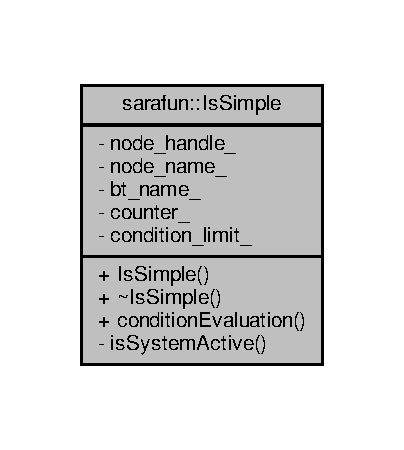
\includegraphics[width=194pt]{de/d41/classsarafun_1_1IsSimple__coll__graph}
\end{center}
\end{figure}
\subsection*{Public Member Functions}
\begin{DoxyCompactItemize}
\item 
\hyperlink{classsarafun_1_1IsSimple_a299c558037426826c95bfc54dbe1a399_a299c558037426826c95bfc54dbe1a399}{Is\-Simple} (std\-::string node\-\_\-name, std\-::string bt\-\_\-name)
\item 
\hyperlink{classsarafun_1_1IsSimple_a90b55180452143b098bfa0f5a184ee58_a90b55180452143b098bfa0f5a184ee58}{$\sim$\-Is\-Simple} ()
\item 
bool \hyperlink{classsarafun_1_1IsSimple_aa57bb3baf9d3ac955e5fdfd5351d45a0_aa57bb3baf9d3ac955e5fdfd5351d45a0}{condition\-Evaluation} ()
\end{DoxyCompactItemize}
\subsection*{Private Member Functions}
\begin{DoxyCompactItemize}
\item 
bool \hyperlink{classsarafun_1_1IsSimple_ac90630b4194e090dfe1e93e7f442576c_ac90630b4194e090dfe1e93e7f442576c}{is\-System\-Active} ()
\end{DoxyCompactItemize}
\subsection*{Private Attributes}
\begin{DoxyCompactItemize}
\item 
ros\-::\-Node\-Handle \hyperlink{classsarafun_1_1IsSimple_a461e5f5f34c94f31f81c11ebd5ccbdc3_a461e5f5f34c94f31f81c11ebd5ccbdc3}{node\-\_\-handle\-\_\-}
\item 
std\-::string \hyperlink{classsarafun_1_1IsSimple_a93a14fccdb5329357b784cb6eb71e2e1_a93a14fccdb5329357b784cb6eb71e2e1}{node\-\_\-name\-\_\-}
\item 
std\-::string \hyperlink{classsarafun_1_1IsSimple_a880440b230fe9b00d396905dbe4dfbc6_a880440b230fe9b00d396905dbe4dfbc6}{bt\-\_\-name\-\_\-}
\item 
int \hyperlink{classsarafun_1_1IsSimple_a57504174276eda97908a4e48b3625a97_a57504174276eda97908a4e48b3625a97}{counter\-\_\-}
\item 
int \hyperlink{classsarafun_1_1IsSimple_aa02f0e66054f68dccf7cc78c763c7141_aa02f0e66054f68dccf7cc78c763c7141}{condition\-\_\-limit\-\_\-}
\end{DoxyCompactItemize}


\subsection{Detailed Description}


Definition at line 8 of file Is\-Simple.\-h.



\subsection{Constructor \& Destructor Documentation}
\hypertarget{classsarafun_1_1IsSimple_a299c558037426826c95bfc54dbe1a399_a299c558037426826c95bfc54dbe1a399}{\index{sarafun\-::\-Is\-Simple@{sarafun\-::\-Is\-Simple}!Is\-Simple@{Is\-Simple}}
\index{Is\-Simple@{Is\-Simple}!sarafun::IsSimple@{sarafun\-::\-Is\-Simple}}
\subsubsection[{Is\-Simple}]{\setlength{\rightskip}{0pt plus 5cm}sarafun\-::\-Is\-Simple\-::\-Is\-Simple (
\begin{DoxyParamCaption}
\item[{std\-::string}]{node\-\_\-name, }
\item[{std\-::string}]{bt\-\_\-name}
\end{DoxyParamCaption}
)\hspace{0.3cm}{\ttfamily [inline]}}}\label{classsarafun_1_1IsSimple_a299c558037426826c95bfc54dbe1a399_a299c558037426826c95bfc54dbe1a399}


Definition at line 10 of file Is\-Simple.\-h.



References bt\-\_\-name\-\_\-, condition\-\_\-limit\-\_\-, counter\-\_\-, and node\-\_\-handle\-\_\-.

\hypertarget{classsarafun_1_1IsSimple_a90b55180452143b098bfa0f5a184ee58_a90b55180452143b098bfa0f5a184ee58}{\index{sarafun\-::\-Is\-Simple@{sarafun\-::\-Is\-Simple}!$\sim$\-Is\-Simple@{$\sim$\-Is\-Simple}}
\index{$\sim$\-Is\-Simple@{$\sim$\-Is\-Simple}!sarafun::IsSimple@{sarafun\-::\-Is\-Simple}}
\subsubsection[{$\sim$\-Is\-Simple}]{\setlength{\rightskip}{0pt plus 5cm}sarafun\-::\-Is\-Simple\-::$\sim$\-Is\-Simple (
\begin{DoxyParamCaption}
{}
\end{DoxyParamCaption}
)\hspace{0.3cm}{\ttfamily [inline]}}}\label{classsarafun_1_1IsSimple_a90b55180452143b098bfa0f5a184ee58_a90b55180452143b098bfa0f5a184ee58}


Definition at line 17 of file Is\-Simple.\-h.



\subsection{Member Function Documentation}
\hypertarget{classsarafun_1_1IsSimple_aa57bb3baf9d3ac955e5fdfd5351d45a0_aa57bb3baf9d3ac955e5fdfd5351d45a0}{\index{sarafun\-::\-Is\-Simple@{sarafun\-::\-Is\-Simple}!condition\-Evaluation@{condition\-Evaluation}}
\index{condition\-Evaluation@{condition\-Evaluation}!sarafun::IsSimple@{sarafun\-::\-Is\-Simple}}
\subsubsection[{condition\-Evaluation}]{\setlength{\rightskip}{0pt plus 5cm}bool sarafun\-::\-Is\-Simple\-::condition\-Evaluation (
\begin{DoxyParamCaption}
{}
\end{DoxyParamCaption}
)}}\label{classsarafun_1_1IsSimple_aa57bb3baf9d3ac955e5fdfd5351d45a0_aa57bb3baf9d3ac955e5fdfd5351d45a0}


Definition at line 20 of file Is\-Simple.\-cpp.



References bt\-\_\-name\-\_\-, condition\-\_\-limit\-\_\-, counter\-\_\-, and is\-System\-Active().



Here is the call graph for this function\-:\nopagebreak
\begin{figure}[H]
\begin{center}
\leavevmode
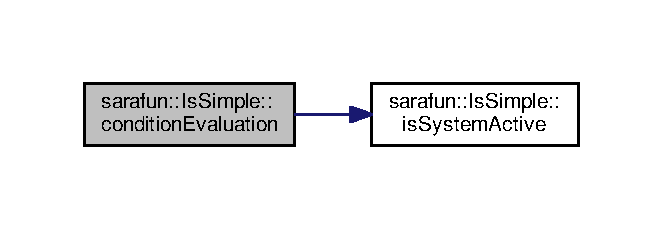
\includegraphics[width=318pt]{dc/d18/classsarafun_1_1IsSimple_aa57bb3baf9d3ac955e5fdfd5351d45a0_aa57bb3baf9d3ac955e5fdfd5351d45a0_cgraph}
\end{center}
\end{figure}


\hypertarget{classsarafun_1_1IsSimple_ac90630b4194e090dfe1e93e7f442576c_ac90630b4194e090dfe1e93e7f442576c}{\index{sarafun\-::\-Is\-Simple@{sarafun\-::\-Is\-Simple}!is\-System\-Active@{is\-System\-Active}}
\index{is\-System\-Active@{is\-System\-Active}!sarafun::IsSimple@{sarafun\-::\-Is\-Simple}}
\subsubsection[{is\-System\-Active}]{\setlength{\rightskip}{0pt plus 5cm}bool sarafun\-::\-Is\-Simple\-::is\-System\-Active (
\begin{DoxyParamCaption}
{}
\end{DoxyParamCaption}
)\hspace{0.3cm}{\ttfamily [private]}}}\label{classsarafun_1_1IsSimple_ac90630b4194e090dfe1e93e7f442576c_ac90630b4194e090dfe1e93e7f442576c}


Definition at line 5 of file Is\-Simple.\-cpp.



Referenced by condition\-Evaluation().



\subsection{Field Documentation}
\hypertarget{classsarafun_1_1IsSimple_a880440b230fe9b00d396905dbe4dfbc6_a880440b230fe9b00d396905dbe4dfbc6}{\index{sarafun\-::\-Is\-Simple@{sarafun\-::\-Is\-Simple}!bt\-\_\-name\-\_\-@{bt\-\_\-name\-\_\-}}
\index{bt\-\_\-name\-\_\-@{bt\-\_\-name\-\_\-}!sarafun::IsSimple@{sarafun\-::\-Is\-Simple}}
\subsubsection[{bt\-\_\-name\-\_\-}]{\setlength{\rightskip}{0pt plus 5cm}std\-::string sarafun\-::\-Is\-Simple\-::bt\-\_\-name\-\_\-\hspace{0.3cm}{\ttfamily [private]}}}\label{classsarafun_1_1IsSimple_a880440b230fe9b00d396905dbe4dfbc6_a880440b230fe9b00d396905dbe4dfbc6}


Definition at line 24 of file Is\-Simple.\-h.



Referenced by condition\-Evaluation(), and Is\-Simple().

\hypertarget{classsarafun_1_1IsSimple_aa02f0e66054f68dccf7cc78c763c7141_aa02f0e66054f68dccf7cc78c763c7141}{\index{sarafun\-::\-Is\-Simple@{sarafun\-::\-Is\-Simple}!condition\-\_\-limit\-\_\-@{condition\-\_\-limit\-\_\-}}
\index{condition\-\_\-limit\-\_\-@{condition\-\_\-limit\-\_\-}!sarafun::IsSimple@{sarafun\-::\-Is\-Simple}}
\subsubsection[{condition\-\_\-limit\-\_\-}]{\setlength{\rightskip}{0pt plus 5cm}int sarafun\-::\-Is\-Simple\-::condition\-\_\-limit\-\_\-\hspace{0.3cm}{\ttfamily [private]}}}\label{classsarafun_1_1IsSimple_aa02f0e66054f68dccf7cc78c763c7141_aa02f0e66054f68dccf7cc78c763c7141}


Definition at line 26 of file Is\-Simple.\-h.



Referenced by condition\-Evaluation(), and Is\-Simple().

\hypertarget{classsarafun_1_1IsSimple_a57504174276eda97908a4e48b3625a97_a57504174276eda97908a4e48b3625a97}{\index{sarafun\-::\-Is\-Simple@{sarafun\-::\-Is\-Simple}!counter\-\_\-@{counter\-\_\-}}
\index{counter\-\_\-@{counter\-\_\-}!sarafun::IsSimple@{sarafun\-::\-Is\-Simple}}
\subsubsection[{counter\-\_\-}]{\setlength{\rightskip}{0pt plus 5cm}int sarafun\-::\-Is\-Simple\-::counter\-\_\-\hspace{0.3cm}{\ttfamily [private]}}}\label{classsarafun_1_1IsSimple_a57504174276eda97908a4e48b3625a97_a57504174276eda97908a4e48b3625a97}


Definition at line 26 of file Is\-Simple.\-h.



Referenced by condition\-Evaluation(), and Is\-Simple().

\hypertarget{classsarafun_1_1IsSimple_a461e5f5f34c94f31f81c11ebd5ccbdc3_a461e5f5f34c94f31f81c11ebd5ccbdc3}{\index{sarafun\-::\-Is\-Simple@{sarafun\-::\-Is\-Simple}!node\-\_\-handle\-\_\-@{node\-\_\-handle\-\_\-}}
\index{node\-\_\-handle\-\_\-@{node\-\_\-handle\-\_\-}!sarafun::IsSimple@{sarafun\-::\-Is\-Simple}}
\subsubsection[{node\-\_\-handle\-\_\-}]{\setlength{\rightskip}{0pt plus 5cm}ros\-::\-Node\-Handle sarafun\-::\-Is\-Simple\-::node\-\_\-handle\-\_\-\hspace{0.3cm}{\ttfamily [private]}}}\label{classsarafun_1_1IsSimple_a461e5f5f34c94f31f81c11ebd5ccbdc3_a461e5f5f34c94f31f81c11ebd5ccbdc3}


Definition at line 22 of file Is\-Simple.\-h.



Referenced by Is\-Simple().

\hypertarget{classsarafun_1_1IsSimple_a93a14fccdb5329357b784cb6eb71e2e1_a93a14fccdb5329357b784cb6eb71e2e1}{\index{sarafun\-::\-Is\-Simple@{sarafun\-::\-Is\-Simple}!node\-\_\-name\-\_\-@{node\-\_\-name\-\_\-}}
\index{node\-\_\-name\-\_\-@{node\-\_\-name\-\_\-}!sarafun::IsSimple@{sarafun\-::\-Is\-Simple}}
\subsubsection[{node\-\_\-name\-\_\-}]{\setlength{\rightskip}{0pt plus 5cm}std\-::string sarafun\-::\-Is\-Simple\-::node\-\_\-name\-\_\-\hspace{0.3cm}{\ttfamily [private]}}}\label{classsarafun_1_1IsSimple_a93a14fccdb5329357b784cb6eb71e2e1_a93a14fccdb5329357b784cb6eb71e2e1}


Definition at line 23 of file Is\-Simple.\-h.



The documentation for this class was generated from the following files\-:\begin{DoxyCompactItemize}
\item 
Is\-Simple.\-h\item 
Is\-Simple.\-cpp\end{DoxyCompactItemize}

\hypertarget{classnlohmann_1_1basic__json_1_1iterator}{\section{nlohmann\-:\-:basic\-\_\-json$<$ Object\-Type, Array\-Type, String\-Type, Boolean\-Type, Number\-Integer\-Type, Number\-Unsigned\-Type, Number\-Float\-Type, Allocator\-Type $>$\-:\-:iterator Class Reference}
\label{classnlohmann_1_1basic__json_1_1iterator}\index{nlohmann\-::basic\-\_\-json$<$ Object\-Type, Array\-Type, String\-Type, Boolean\-Type, Number\-Integer\-Type, Number\-Unsigned\-Type, Number\-Float\-Type, Allocator\-Type $>$\-::iterator@{nlohmann\-::basic\-\_\-json$<$ Object\-Type, Array\-Type, String\-Type, Boolean\-Type, Number\-Integer\-Type, Number\-Unsigned\-Type, Number\-Float\-Type, Allocator\-Type $>$\-::iterator}}
}


a mutable random access iterator for the \hyperlink{classnlohmann_1_1basic__json}{basic\-\_\-json} class  




{\ttfamily \#include $<$json.\-hpp$>$}

Inheritance diagram for nlohmann\-:\-:basic\-\_\-json$<$ Object\-Type, Array\-Type, String\-Type, Boolean\-Type, Number\-Integer\-Type, Number\-Unsigned\-Type, Number\-Float\-Type, Allocator\-Type $>$\-:\-:iterator\-:\begin{figure}[H]
\begin{center}
\leavevmode
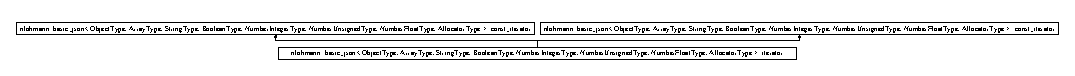
\includegraphics[height=0.568528cm]{d4/d0f/classnlohmann_1_1basic__json_1_1iterator}
\end{center}
\end{figure}
\subsection*{Public Types}
\begin{DoxyCompactItemize}
\item 
\hypertarget{classnlohmann_1_1basic__json_1_1iterator_ac48754e4dc48d65d95294bd170dcd857_ac48754e4dc48d65d95294bd170dcd857}{using {\bfseries base\-\_\-iterator} = \hyperlink{classnlohmann_1_1basic__json_1_1const__iterator}{const\-\_\-iterator}}\label{classnlohmann_1_1basic__json_1_1iterator_ac48754e4dc48d65d95294bd170dcd857_ac48754e4dc48d65d95294bd170dcd857}

\item 
\hypertarget{classnlohmann_1_1basic__json_1_1iterator_a3aae1df93a78b201d98e178c1c7d02a7_a3aae1df93a78b201d98e178c1c7d02a7}{using {\bfseries pointer} = typename \hyperlink{classnlohmann_1_1basic__json_a9d1b58099dc64695fcf2847ab0b2a7c7_a9d1b58099dc64695fcf2847ab0b2a7c7}{basic\-\_\-json\-::pointer}}\label{classnlohmann_1_1basic__json_1_1iterator_a3aae1df93a78b201d98e178c1c7d02a7_a3aae1df93a78b201d98e178c1c7d02a7}

\item 
\hypertarget{classnlohmann_1_1basic__json_1_1iterator_a97aff5d71246774267a81066460dd1cf_a97aff5d71246774267a81066460dd1cf}{using {\bfseries reference} = typename \hyperlink{classnlohmann_1_1basic__json_a3ec8e17be8732fe436e9d6733f52b7a3_a3ec8e17be8732fe436e9d6733f52b7a3}{basic\-\_\-json\-::reference}}\label{classnlohmann_1_1basic__json_1_1iterator_a97aff5d71246774267a81066460dd1cf_a97aff5d71246774267a81066460dd1cf}

\item 
\hypertarget{classnlohmann_1_1basic__json_1_1iterator_ac48754e4dc48d65d95294bd170dcd857_ac48754e4dc48d65d95294bd170dcd857}{using {\bfseries base\-\_\-iterator} = \hyperlink{classnlohmann_1_1basic__json_1_1const__iterator}{const\-\_\-iterator}}\label{classnlohmann_1_1basic__json_1_1iterator_ac48754e4dc48d65d95294bd170dcd857_ac48754e4dc48d65d95294bd170dcd857}

\item 
\hypertarget{classnlohmann_1_1basic__json_1_1iterator_a3aae1df93a78b201d98e178c1c7d02a7_a3aae1df93a78b201d98e178c1c7d02a7}{using {\bfseries pointer} = typename \hyperlink{classnlohmann_1_1basic__json_a9d1b58099dc64695fcf2847ab0b2a7c7_a9d1b58099dc64695fcf2847ab0b2a7c7}{basic\-\_\-json\-::pointer}}\label{classnlohmann_1_1basic__json_1_1iterator_a3aae1df93a78b201d98e178c1c7d02a7_a3aae1df93a78b201d98e178c1c7d02a7}

\item 
\hypertarget{classnlohmann_1_1basic__json_1_1iterator_a97aff5d71246774267a81066460dd1cf_a97aff5d71246774267a81066460dd1cf}{using {\bfseries reference} = typename \hyperlink{classnlohmann_1_1basic__json_a3ec8e17be8732fe436e9d6733f52b7a3_a3ec8e17be8732fe436e9d6733f52b7a3}{basic\-\_\-json\-::reference}}\label{classnlohmann_1_1basic__json_1_1iterator_a97aff5d71246774267a81066460dd1cf_a97aff5d71246774267a81066460dd1cf}

\end{DoxyCompactItemize}
\subsection*{Public Member Functions}
\begin{DoxyCompactItemize}
\item 
\hypertarget{classnlohmann_1_1basic__json_1_1iterator_a47fb2dbbbfaf65c0ccfa99aeaed920a1_a47fb2dbbbfaf65c0ccfa99aeaed920a1}{\hyperlink{classnlohmann_1_1basic__json_1_1iterator_a47fb2dbbbfaf65c0ccfa99aeaed920a1_a47fb2dbbbfaf65c0ccfa99aeaed920a1}{iterator} ()=default}\label{classnlohmann_1_1basic__json_1_1iterator_a47fb2dbbbfaf65c0ccfa99aeaed920a1_a47fb2dbbbfaf65c0ccfa99aeaed920a1}

\begin{DoxyCompactList}\small\item\em default constructor \end{DoxyCompactList}\item 
\hypertarget{classnlohmann_1_1basic__json_1_1iterator_a085fe0d8cf459b5b1ae7b518b933ae7d_a085fe0d8cf459b5b1ae7b518b933ae7d}{\hyperlink{classnlohmann_1_1basic__json_1_1iterator_a085fe0d8cf459b5b1ae7b518b933ae7d_a085fe0d8cf459b5b1ae7b518b933ae7d}{iterator} (\hyperlink{classnlohmann_1_1basic__json_1_1const__iterator_a1da96fc3054d547e7706d3a2f073f389_a1da96fc3054d547e7706d3a2f073f389}{pointer} \hyperlink{classnlohmann_1_1basic__json_ad25b2f8c21e241e2d63455537a9294ff_ad25b2f8c21e241e2d63455537a9294ff}{object}) noexcept}\label{classnlohmann_1_1basic__json_1_1iterator_a085fe0d8cf459b5b1ae7b518b933ae7d_a085fe0d8cf459b5b1ae7b518b933ae7d}

\begin{DoxyCompactList}\small\item\em constructor for a given J\-S\-O\-N instance \end{DoxyCompactList}\item 
\hypertarget{classnlohmann_1_1basic__json_1_1iterator_a1de0975e812c83e74d118b3e1063f335_a1de0975e812c83e74d118b3e1063f335}{\hyperlink{classnlohmann_1_1basic__json_1_1iterator_a1de0975e812c83e74d118b3e1063f335_a1de0975e812c83e74d118b3e1063f335}{iterator} (const \hyperlink{classnlohmann_1_1basic__json_1_1iterator}{iterator} \&other) noexcept}\label{classnlohmann_1_1basic__json_1_1iterator_a1de0975e812c83e74d118b3e1063f335_a1de0975e812c83e74d118b3e1063f335}

\begin{DoxyCompactList}\small\item\em copy constructor \end{DoxyCompactList}\item 
\hypertarget{classnlohmann_1_1basic__json_1_1iterator_a28e1e3ea6f52ab57f1a2fd98f6ab5d9c_a28e1e3ea6f52ab57f1a2fd98f6ab5d9c}{\hyperlink{classnlohmann_1_1basic__json_1_1iterator}{iterator} \& \hyperlink{classnlohmann_1_1basic__json_1_1iterator_a28e1e3ea6f52ab57f1a2fd98f6ab5d9c_a28e1e3ea6f52ab57f1a2fd98f6ab5d9c}{operator=} (\hyperlink{classnlohmann_1_1basic__json_1_1iterator}{iterator} other) noexcept(std\-::is\-\_\-nothrow\-\_\-move\-\_\-constructible$<$ \hyperlink{classnlohmann_1_1basic__json_1_1const__iterator_a1da96fc3054d547e7706d3a2f073f389_a1da96fc3054d547e7706d3a2f073f389}{pointer} $>$\-::\hyperlink{classnlohmann_1_1basic__json_1_1iterator_a8ffbf287736048e683f58306fdb8701f_a8ffbf287736048e683f58306fdb8701f}{value} andstd\-::is\-\_\-nothrow\-\_\-move\-\_\-assignable$<$ \hyperlink{classnlohmann_1_1basic__json_1_1const__iterator_a1da96fc3054d547e7706d3a2f073f389_a1da96fc3054d547e7706d3a2f073f389}{pointer} $>$\-::\hyperlink{classnlohmann_1_1basic__json_1_1iterator_a8ffbf287736048e683f58306fdb8701f_a8ffbf287736048e683f58306fdb8701f}{value} andstd\-::is\-\_\-nothrow\-\_\-move\-\_\-constructible$<$ \hyperlink{structnlohmann_1_1basic__json_1_1internal__iterator}{internal\-\_\-iterator} $>$\-::\hyperlink{classnlohmann_1_1basic__json_1_1iterator_a8ffbf287736048e683f58306fdb8701f_a8ffbf287736048e683f58306fdb8701f}{value} andstd\-::is\-\_\-nothrow\-\_\-move\-\_\-assignable$<$ \hyperlink{structnlohmann_1_1basic__json_1_1internal__iterator}{internal\-\_\-iterator} $>$\-::\hyperlink{classnlohmann_1_1basic__json_1_1iterator_a8ffbf287736048e683f58306fdb8701f_a8ffbf287736048e683f58306fdb8701f}{value})}\label{classnlohmann_1_1basic__json_1_1iterator_a28e1e3ea6f52ab57f1a2fd98f6ab5d9c_a28e1e3ea6f52ab57f1a2fd98f6ab5d9c}

\begin{DoxyCompactList}\small\item\em copy assignment \end{DoxyCompactList}\item 
\hypertarget{classnlohmann_1_1basic__json_1_1iterator_acbd82115f9232c3d3b5dacc78315b9da_acbd82115f9232c3d3b5dacc78315b9da}{\hyperlink{classnlohmann_1_1basic__json_1_1const__iterator_aefd248cac6493eed1e6ff53ba6a63eb2_aefd248cac6493eed1e6ff53ba6a63eb2}{reference} \hyperlink{classnlohmann_1_1basic__json_1_1iterator_acbd82115f9232c3d3b5dacc78315b9da_acbd82115f9232c3d3b5dacc78315b9da}{operator$\ast$} () const }\label{classnlohmann_1_1basic__json_1_1iterator_acbd82115f9232c3d3b5dacc78315b9da_acbd82115f9232c3d3b5dacc78315b9da}

\begin{DoxyCompactList}\small\item\em return a reference to the value pointed to by the iterator \end{DoxyCompactList}\item 
\hypertarget{classnlohmann_1_1basic__json_1_1iterator_a8de46badb5b2177c85c672a71bcca017_a8de46badb5b2177c85c672a71bcca017}{\hyperlink{classnlohmann_1_1basic__json_1_1const__iterator_a1da96fc3054d547e7706d3a2f073f389_a1da96fc3054d547e7706d3a2f073f389}{pointer} \hyperlink{classnlohmann_1_1basic__json_1_1iterator_a8de46badb5b2177c85c672a71bcca017_a8de46badb5b2177c85c672a71bcca017}{operator-\/$>$} () const }\label{classnlohmann_1_1basic__json_1_1iterator_a8de46badb5b2177c85c672a71bcca017_a8de46badb5b2177c85c672a71bcca017}

\begin{DoxyCompactList}\small\item\em dereference the iterator \end{DoxyCompactList}\item 
\hypertarget{classnlohmann_1_1basic__json_1_1iterator_a2943e49b3d88e6ee5793c5923ab2ede9_a2943e49b3d88e6ee5793c5923ab2ede9}{\hyperlink{classnlohmann_1_1basic__json_1_1iterator}{iterator} \hyperlink{classnlohmann_1_1basic__json_1_1iterator_a2943e49b3d88e6ee5793c5923ab2ede9_a2943e49b3d88e6ee5793c5923ab2ede9}{operator++} (int)}\label{classnlohmann_1_1basic__json_1_1iterator_a2943e49b3d88e6ee5793c5923ab2ede9_a2943e49b3d88e6ee5793c5923ab2ede9}

\begin{DoxyCompactList}\small\item\em post-\/increment (it++) \end{DoxyCompactList}\item 
\hypertarget{classnlohmann_1_1basic__json_1_1iterator_a050b7fa21051ea57e5b0cc03668b5d4a_a050b7fa21051ea57e5b0cc03668b5d4a}{\hyperlink{classnlohmann_1_1basic__json_1_1iterator}{iterator} \& \hyperlink{classnlohmann_1_1basic__json_1_1iterator_a050b7fa21051ea57e5b0cc03668b5d4a_a050b7fa21051ea57e5b0cc03668b5d4a}{operator++} ()}\label{classnlohmann_1_1basic__json_1_1iterator_a050b7fa21051ea57e5b0cc03668b5d4a_a050b7fa21051ea57e5b0cc03668b5d4a}

\begin{DoxyCompactList}\small\item\em pre-\/increment (++it) \end{DoxyCompactList}\item 
\hypertarget{classnlohmann_1_1basic__json_1_1iterator_ab4f238aa5fcf452b1884b748b0395b1f_ab4f238aa5fcf452b1884b748b0395b1f}{\hyperlink{classnlohmann_1_1basic__json_1_1iterator}{iterator} \hyperlink{classnlohmann_1_1basic__json_1_1iterator_ab4f238aa5fcf452b1884b748b0395b1f_ab4f238aa5fcf452b1884b748b0395b1f}{operator-\/-\/} (int)}\label{classnlohmann_1_1basic__json_1_1iterator_ab4f238aa5fcf452b1884b748b0395b1f_ab4f238aa5fcf452b1884b748b0395b1f}

\begin{DoxyCompactList}\small\item\em post-\/decrement (it--) \end{DoxyCompactList}\item 
\hypertarget{classnlohmann_1_1basic__json_1_1iterator_ab3679dc63b3a59edb98b1c2b96d8683c_ab3679dc63b3a59edb98b1c2b96d8683c}{\hyperlink{classnlohmann_1_1basic__json_1_1iterator}{iterator} \& \hyperlink{classnlohmann_1_1basic__json_1_1iterator_ab3679dc63b3a59edb98b1c2b96d8683c_ab3679dc63b3a59edb98b1c2b96d8683c}{operator-\/-\/} ()}\label{classnlohmann_1_1basic__json_1_1iterator_ab3679dc63b3a59edb98b1c2b96d8683c_ab3679dc63b3a59edb98b1c2b96d8683c}

\begin{DoxyCompactList}\small\item\em pre-\/decrement (--it) \end{DoxyCompactList}\item 
\hypertarget{classnlohmann_1_1basic__json_1_1iterator_ae0c848dbc0af1cde15771d45d775b27c_ae0c848dbc0af1cde15771d45d775b27c}{\hyperlink{classnlohmann_1_1basic__json_1_1iterator}{iterator} \& \hyperlink{classnlohmann_1_1basic__json_1_1iterator_ae0c848dbc0af1cde15771d45d775b27c_ae0c848dbc0af1cde15771d45d775b27c}{operator+=} (\hyperlink{classnlohmann_1_1basic__json_1_1const__iterator_a49d7c3e9ef3280df03052cce988b792f_a49d7c3e9ef3280df03052cce988b792f}{difference\-\_\-type} i)}\label{classnlohmann_1_1basic__json_1_1iterator_ae0c848dbc0af1cde15771d45d775b27c_ae0c848dbc0af1cde15771d45d775b27c}

\begin{DoxyCompactList}\small\item\em add to iterator \end{DoxyCompactList}\item 
\hypertarget{classnlohmann_1_1basic__json_1_1iterator_afe86d48d3e4e5ebdaaec162b3cf0e95c_afe86d48d3e4e5ebdaaec162b3cf0e95c}{\hyperlink{classnlohmann_1_1basic__json_1_1iterator}{iterator} \& \hyperlink{classnlohmann_1_1basic__json_1_1iterator_afe86d48d3e4e5ebdaaec162b3cf0e95c_afe86d48d3e4e5ebdaaec162b3cf0e95c}{operator-\/=} (\hyperlink{classnlohmann_1_1basic__json_1_1const__iterator_a49d7c3e9ef3280df03052cce988b792f_a49d7c3e9ef3280df03052cce988b792f}{difference\-\_\-type} i)}\label{classnlohmann_1_1basic__json_1_1iterator_afe86d48d3e4e5ebdaaec162b3cf0e95c_afe86d48d3e4e5ebdaaec162b3cf0e95c}

\begin{DoxyCompactList}\small\item\em subtract from iterator \end{DoxyCompactList}\item 
\hypertarget{classnlohmann_1_1basic__json_1_1iterator_a56952f8d5702541f0d88e6a764d2ae36_a56952f8d5702541f0d88e6a764d2ae36}{\hyperlink{classnlohmann_1_1basic__json_1_1iterator}{iterator} \hyperlink{classnlohmann_1_1basic__json_1_1iterator_a56952f8d5702541f0d88e6a764d2ae36_a56952f8d5702541f0d88e6a764d2ae36}{operator+} (\hyperlink{classnlohmann_1_1basic__json_1_1const__iterator_a49d7c3e9ef3280df03052cce988b792f_a49d7c3e9ef3280df03052cce988b792f}{difference\-\_\-type} i)}\label{classnlohmann_1_1basic__json_1_1iterator_a56952f8d5702541f0d88e6a764d2ae36_a56952f8d5702541f0d88e6a764d2ae36}

\begin{DoxyCompactList}\small\item\em add to iterator \end{DoxyCompactList}\item 
\hypertarget{classnlohmann_1_1basic__json_1_1iterator_a790f550ff168095c83c2e459c575916c_a790f550ff168095c83c2e459c575916c}{\hyperlink{classnlohmann_1_1basic__json_1_1iterator}{iterator} \hyperlink{classnlohmann_1_1basic__json_1_1iterator_a790f550ff168095c83c2e459c575916c_a790f550ff168095c83c2e459c575916c}{operator-\/} (\hyperlink{classnlohmann_1_1basic__json_1_1const__iterator_a49d7c3e9ef3280df03052cce988b792f_a49d7c3e9ef3280df03052cce988b792f}{difference\-\_\-type} i)}\label{classnlohmann_1_1basic__json_1_1iterator_a790f550ff168095c83c2e459c575916c_a790f550ff168095c83c2e459c575916c}

\begin{DoxyCompactList}\small\item\em subtract from iterator \end{DoxyCompactList}\item 
\hypertarget{classnlohmann_1_1basic__json_1_1iterator_a9f3940ac5fb2c6ff8045ed59b8a0866f_a9f3940ac5fb2c6ff8045ed59b8a0866f}{\hyperlink{classnlohmann_1_1basic__json_1_1const__iterator_a49d7c3e9ef3280df03052cce988b792f_a49d7c3e9ef3280df03052cce988b792f}{difference\-\_\-type} \hyperlink{classnlohmann_1_1basic__json_1_1iterator_a9f3940ac5fb2c6ff8045ed59b8a0866f_a9f3940ac5fb2c6ff8045ed59b8a0866f}{operator-\/} (const \hyperlink{classnlohmann_1_1basic__json_1_1iterator}{iterator} \&other) const }\label{classnlohmann_1_1basic__json_1_1iterator_a9f3940ac5fb2c6ff8045ed59b8a0866f_a9f3940ac5fb2c6ff8045ed59b8a0866f}

\begin{DoxyCompactList}\small\item\em return difference \end{DoxyCompactList}\item 
\hypertarget{classnlohmann_1_1basic__json_1_1iterator_a7e01532727c10f87926dac4eb8e170f4_a7e01532727c10f87926dac4eb8e170f4}{\hyperlink{classnlohmann_1_1basic__json_1_1const__iterator_aefd248cac6493eed1e6ff53ba6a63eb2_aefd248cac6493eed1e6ff53ba6a63eb2}{reference} \hyperlink{classnlohmann_1_1basic__json_1_1iterator_a7e01532727c10f87926dac4eb8e170f4_a7e01532727c10f87926dac4eb8e170f4}{operator\mbox{[}$\,$\mbox{]}} (\hyperlink{classnlohmann_1_1basic__json_1_1const__iterator_a49d7c3e9ef3280df03052cce988b792f_a49d7c3e9ef3280df03052cce988b792f}{difference\-\_\-type} n) const }\label{classnlohmann_1_1basic__json_1_1iterator_a7e01532727c10f87926dac4eb8e170f4_a7e01532727c10f87926dac4eb8e170f4}

\begin{DoxyCompactList}\small\item\em access to successor \end{DoxyCompactList}\item 
\hypertarget{classnlohmann_1_1basic__json_1_1iterator_a8ffbf287736048e683f58306fdb8701f_a8ffbf287736048e683f58306fdb8701f}{\hyperlink{classnlohmann_1_1basic__json_1_1const__iterator_aefd248cac6493eed1e6ff53ba6a63eb2_aefd248cac6493eed1e6ff53ba6a63eb2}{reference} \hyperlink{classnlohmann_1_1basic__json_1_1iterator_a8ffbf287736048e683f58306fdb8701f_a8ffbf287736048e683f58306fdb8701f}{value} () const }\label{classnlohmann_1_1basic__json_1_1iterator_a8ffbf287736048e683f58306fdb8701f_a8ffbf287736048e683f58306fdb8701f}

\begin{DoxyCompactList}\small\item\em return the value of an iterator \end{DoxyCompactList}\item 
\hypertarget{classnlohmann_1_1basic__json_1_1iterator_a47fb2dbbbfaf65c0ccfa99aeaed920a1_a47fb2dbbbfaf65c0ccfa99aeaed920a1}{\hyperlink{classnlohmann_1_1basic__json_1_1iterator_a47fb2dbbbfaf65c0ccfa99aeaed920a1_a47fb2dbbbfaf65c0ccfa99aeaed920a1}{iterator} ()=default}\label{classnlohmann_1_1basic__json_1_1iterator_a47fb2dbbbfaf65c0ccfa99aeaed920a1_a47fb2dbbbfaf65c0ccfa99aeaed920a1}

\begin{DoxyCompactList}\small\item\em default constructor \end{DoxyCompactList}\item 
\hypertarget{classnlohmann_1_1basic__json_1_1iterator_a085fe0d8cf459b5b1ae7b518b933ae7d_a085fe0d8cf459b5b1ae7b518b933ae7d}{\hyperlink{classnlohmann_1_1basic__json_1_1iterator_a085fe0d8cf459b5b1ae7b518b933ae7d_a085fe0d8cf459b5b1ae7b518b933ae7d}{iterator} (\hyperlink{classnlohmann_1_1basic__json_1_1const__iterator_a1da96fc3054d547e7706d3a2f073f389_a1da96fc3054d547e7706d3a2f073f389}{pointer} \hyperlink{classnlohmann_1_1basic__json_ad25b2f8c21e241e2d63455537a9294ff_ad25b2f8c21e241e2d63455537a9294ff}{object}) noexcept}\label{classnlohmann_1_1basic__json_1_1iterator_a085fe0d8cf459b5b1ae7b518b933ae7d_a085fe0d8cf459b5b1ae7b518b933ae7d}

\begin{DoxyCompactList}\small\item\em constructor for a given J\-S\-O\-N instance \end{DoxyCompactList}\item 
\hypertarget{classnlohmann_1_1basic__json_1_1iterator_a1de0975e812c83e74d118b3e1063f335_a1de0975e812c83e74d118b3e1063f335}{\hyperlink{classnlohmann_1_1basic__json_1_1iterator_a1de0975e812c83e74d118b3e1063f335_a1de0975e812c83e74d118b3e1063f335}{iterator} (const \hyperlink{classnlohmann_1_1basic__json_1_1iterator}{iterator} \&other) noexcept}\label{classnlohmann_1_1basic__json_1_1iterator_a1de0975e812c83e74d118b3e1063f335_a1de0975e812c83e74d118b3e1063f335}

\begin{DoxyCompactList}\small\item\em copy constructor \end{DoxyCompactList}\item 
\hypertarget{classnlohmann_1_1basic__json_1_1iterator_a28e1e3ea6f52ab57f1a2fd98f6ab5d9c_a28e1e3ea6f52ab57f1a2fd98f6ab5d9c}{\hyperlink{classnlohmann_1_1basic__json_1_1iterator}{iterator} \& \hyperlink{classnlohmann_1_1basic__json_1_1iterator_a28e1e3ea6f52ab57f1a2fd98f6ab5d9c_a28e1e3ea6f52ab57f1a2fd98f6ab5d9c}{operator=} (\hyperlink{classnlohmann_1_1basic__json_1_1iterator}{iterator} other) noexcept(std\-::is\-\_\-nothrow\-\_\-move\-\_\-constructible$<$ \hyperlink{classnlohmann_1_1basic__json_1_1const__iterator_a1da96fc3054d547e7706d3a2f073f389_a1da96fc3054d547e7706d3a2f073f389}{pointer} $>$\-::\hyperlink{classnlohmann_1_1basic__json_1_1iterator_a8ffbf287736048e683f58306fdb8701f_a8ffbf287736048e683f58306fdb8701f}{value} andstd\-::is\-\_\-nothrow\-\_\-move\-\_\-assignable$<$ \hyperlink{classnlohmann_1_1basic__json_1_1const__iterator_a1da96fc3054d547e7706d3a2f073f389_a1da96fc3054d547e7706d3a2f073f389}{pointer} $>$\-::\hyperlink{classnlohmann_1_1basic__json_1_1iterator_a8ffbf287736048e683f58306fdb8701f_a8ffbf287736048e683f58306fdb8701f}{value} andstd\-::is\-\_\-nothrow\-\_\-move\-\_\-constructible$<$ \hyperlink{structnlohmann_1_1basic__json_1_1internal__iterator}{internal\-\_\-iterator} $>$\-::\hyperlink{classnlohmann_1_1basic__json_1_1iterator_a8ffbf287736048e683f58306fdb8701f_a8ffbf287736048e683f58306fdb8701f}{value} andstd\-::is\-\_\-nothrow\-\_\-move\-\_\-assignable$<$ \hyperlink{structnlohmann_1_1basic__json_1_1internal__iterator}{internal\-\_\-iterator} $>$\-::\hyperlink{classnlohmann_1_1basic__json_1_1iterator_a8ffbf287736048e683f58306fdb8701f_a8ffbf287736048e683f58306fdb8701f}{value})}\label{classnlohmann_1_1basic__json_1_1iterator_a28e1e3ea6f52ab57f1a2fd98f6ab5d9c_a28e1e3ea6f52ab57f1a2fd98f6ab5d9c}

\begin{DoxyCompactList}\small\item\em copy assignment \end{DoxyCompactList}\item 
\hypertarget{classnlohmann_1_1basic__json_1_1iterator_acbd82115f9232c3d3b5dacc78315b9da_acbd82115f9232c3d3b5dacc78315b9da}{\hyperlink{classnlohmann_1_1basic__json_1_1const__iterator_aefd248cac6493eed1e6ff53ba6a63eb2_aefd248cac6493eed1e6ff53ba6a63eb2}{reference} \hyperlink{classnlohmann_1_1basic__json_1_1iterator_acbd82115f9232c3d3b5dacc78315b9da_acbd82115f9232c3d3b5dacc78315b9da}{operator$\ast$} () const }\label{classnlohmann_1_1basic__json_1_1iterator_acbd82115f9232c3d3b5dacc78315b9da_acbd82115f9232c3d3b5dacc78315b9da}

\begin{DoxyCompactList}\small\item\em return a reference to the value pointed to by the iterator \end{DoxyCompactList}\item 
\hypertarget{classnlohmann_1_1basic__json_1_1iterator_a8de46badb5b2177c85c672a71bcca017_a8de46badb5b2177c85c672a71bcca017}{\hyperlink{classnlohmann_1_1basic__json_1_1const__iterator_a1da96fc3054d547e7706d3a2f073f389_a1da96fc3054d547e7706d3a2f073f389}{pointer} \hyperlink{classnlohmann_1_1basic__json_1_1iterator_a8de46badb5b2177c85c672a71bcca017_a8de46badb5b2177c85c672a71bcca017}{operator-\/$>$} () const }\label{classnlohmann_1_1basic__json_1_1iterator_a8de46badb5b2177c85c672a71bcca017_a8de46badb5b2177c85c672a71bcca017}

\begin{DoxyCompactList}\small\item\em dereference the iterator \end{DoxyCompactList}\item 
\hypertarget{classnlohmann_1_1basic__json_1_1iterator_a2943e49b3d88e6ee5793c5923ab2ede9_a2943e49b3d88e6ee5793c5923ab2ede9}{\hyperlink{classnlohmann_1_1basic__json_1_1iterator}{iterator} \hyperlink{classnlohmann_1_1basic__json_1_1iterator_a2943e49b3d88e6ee5793c5923ab2ede9_a2943e49b3d88e6ee5793c5923ab2ede9}{operator++} (int)}\label{classnlohmann_1_1basic__json_1_1iterator_a2943e49b3d88e6ee5793c5923ab2ede9_a2943e49b3d88e6ee5793c5923ab2ede9}

\begin{DoxyCompactList}\small\item\em post-\/increment (it++) \end{DoxyCompactList}\item 
\hypertarget{classnlohmann_1_1basic__json_1_1iterator_a050b7fa21051ea57e5b0cc03668b5d4a_a050b7fa21051ea57e5b0cc03668b5d4a}{\hyperlink{classnlohmann_1_1basic__json_1_1iterator}{iterator} \& \hyperlink{classnlohmann_1_1basic__json_1_1iterator_a050b7fa21051ea57e5b0cc03668b5d4a_a050b7fa21051ea57e5b0cc03668b5d4a}{operator++} ()}\label{classnlohmann_1_1basic__json_1_1iterator_a050b7fa21051ea57e5b0cc03668b5d4a_a050b7fa21051ea57e5b0cc03668b5d4a}

\begin{DoxyCompactList}\small\item\em pre-\/increment (++it) \end{DoxyCompactList}\item 
\hypertarget{classnlohmann_1_1basic__json_1_1iterator_ab4f238aa5fcf452b1884b748b0395b1f_ab4f238aa5fcf452b1884b748b0395b1f}{\hyperlink{classnlohmann_1_1basic__json_1_1iterator}{iterator} \hyperlink{classnlohmann_1_1basic__json_1_1iterator_ab4f238aa5fcf452b1884b748b0395b1f_ab4f238aa5fcf452b1884b748b0395b1f}{operator-\/-\/} (int)}\label{classnlohmann_1_1basic__json_1_1iterator_ab4f238aa5fcf452b1884b748b0395b1f_ab4f238aa5fcf452b1884b748b0395b1f}

\begin{DoxyCompactList}\small\item\em post-\/decrement (it--) \end{DoxyCompactList}\item 
\hypertarget{classnlohmann_1_1basic__json_1_1iterator_ab3679dc63b3a59edb98b1c2b96d8683c_ab3679dc63b3a59edb98b1c2b96d8683c}{\hyperlink{classnlohmann_1_1basic__json_1_1iterator}{iterator} \& \hyperlink{classnlohmann_1_1basic__json_1_1iterator_ab3679dc63b3a59edb98b1c2b96d8683c_ab3679dc63b3a59edb98b1c2b96d8683c}{operator-\/-\/} ()}\label{classnlohmann_1_1basic__json_1_1iterator_ab3679dc63b3a59edb98b1c2b96d8683c_ab3679dc63b3a59edb98b1c2b96d8683c}

\begin{DoxyCompactList}\small\item\em pre-\/decrement (--it) \end{DoxyCompactList}\item 
\hypertarget{classnlohmann_1_1basic__json_1_1iterator_ae0c848dbc0af1cde15771d45d775b27c_ae0c848dbc0af1cde15771d45d775b27c}{\hyperlink{classnlohmann_1_1basic__json_1_1iterator}{iterator} \& \hyperlink{classnlohmann_1_1basic__json_1_1iterator_ae0c848dbc0af1cde15771d45d775b27c_ae0c848dbc0af1cde15771d45d775b27c}{operator+=} (\hyperlink{classnlohmann_1_1basic__json_1_1const__iterator_a49d7c3e9ef3280df03052cce988b792f_a49d7c3e9ef3280df03052cce988b792f}{difference\-\_\-type} i)}\label{classnlohmann_1_1basic__json_1_1iterator_ae0c848dbc0af1cde15771d45d775b27c_ae0c848dbc0af1cde15771d45d775b27c}

\begin{DoxyCompactList}\small\item\em add to iterator \end{DoxyCompactList}\item 
\hypertarget{classnlohmann_1_1basic__json_1_1iterator_afe86d48d3e4e5ebdaaec162b3cf0e95c_afe86d48d3e4e5ebdaaec162b3cf0e95c}{\hyperlink{classnlohmann_1_1basic__json_1_1iterator}{iterator} \& \hyperlink{classnlohmann_1_1basic__json_1_1iterator_afe86d48d3e4e5ebdaaec162b3cf0e95c_afe86d48d3e4e5ebdaaec162b3cf0e95c}{operator-\/=} (\hyperlink{classnlohmann_1_1basic__json_1_1const__iterator_a49d7c3e9ef3280df03052cce988b792f_a49d7c3e9ef3280df03052cce988b792f}{difference\-\_\-type} i)}\label{classnlohmann_1_1basic__json_1_1iterator_afe86d48d3e4e5ebdaaec162b3cf0e95c_afe86d48d3e4e5ebdaaec162b3cf0e95c}

\begin{DoxyCompactList}\small\item\em subtract from iterator \end{DoxyCompactList}\item 
\hypertarget{classnlohmann_1_1basic__json_1_1iterator_a56952f8d5702541f0d88e6a764d2ae36_a56952f8d5702541f0d88e6a764d2ae36}{\hyperlink{classnlohmann_1_1basic__json_1_1iterator}{iterator} \hyperlink{classnlohmann_1_1basic__json_1_1iterator_a56952f8d5702541f0d88e6a764d2ae36_a56952f8d5702541f0d88e6a764d2ae36}{operator+} (\hyperlink{classnlohmann_1_1basic__json_1_1const__iterator_a49d7c3e9ef3280df03052cce988b792f_a49d7c3e9ef3280df03052cce988b792f}{difference\-\_\-type} i)}\label{classnlohmann_1_1basic__json_1_1iterator_a56952f8d5702541f0d88e6a764d2ae36_a56952f8d5702541f0d88e6a764d2ae36}

\begin{DoxyCompactList}\small\item\em add to iterator \end{DoxyCompactList}\item 
\hypertarget{classnlohmann_1_1basic__json_1_1iterator_a790f550ff168095c83c2e459c575916c_a790f550ff168095c83c2e459c575916c}{\hyperlink{classnlohmann_1_1basic__json_1_1iterator}{iterator} \hyperlink{classnlohmann_1_1basic__json_1_1iterator_a790f550ff168095c83c2e459c575916c_a790f550ff168095c83c2e459c575916c}{operator-\/} (\hyperlink{classnlohmann_1_1basic__json_1_1const__iterator_a49d7c3e9ef3280df03052cce988b792f_a49d7c3e9ef3280df03052cce988b792f}{difference\-\_\-type} i)}\label{classnlohmann_1_1basic__json_1_1iterator_a790f550ff168095c83c2e459c575916c_a790f550ff168095c83c2e459c575916c}

\begin{DoxyCompactList}\small\item\em subtract from iterator \end{DoxyCompactList}\item 
\hypertarget{classnlohmann_1_1basic__json_1_1iterator_a9f3940ac5fb2c6ff8045ed59b8a0866f_a9f3940ac5fb2c6ff8045ed59b8a0866f}{\hyperlink{classnlohmann_1_1basic__json_1_1const__iterator_a49d7c3e9ef3280df03052cce988b792f_a49d7c3e9ef3280df03052cce988b792f}{difference\-\_\-type} \hyperlink{classnlohmann_1_1basic__json_1_1iterator_a9f3940ac5fb2c6ff8045ed59b8a0866f_a9f3940ac5fb2c6ff8045ed59b8a0866f}{operator-\/} (const \hyperlink{classnlohmann_1_1basic__json_1_1iterator}{iterator} \&other) const }\label{classnlohmann_1_1basic__json_1_1iterator_a9f3940ac5fb2c6ff8045ed59b8a0866f_a9f3940ac5fb2c6ff8045ed59b8a0866f}

\begin{DoxyCompactList}\small\item\em return difference \end{DoxyCompactList}\item 
\hypertarget{classnlohmann_1_1basic__json_1_1iterator_a7e01532727c10f87926dac4eb8e170f4_a7e01532727c10f87926dac4eb8e170f4}{\hyperlink{classnlohmann_1_1basic__json_1_1const__iterator_aefd248cac6493eed1e6ff53ba6a63eb2_aefd248cac6493eed1e6ff53ba6a63eb2}{reference} \hyperlink{classnlohmann_1_1basic__json_1_1iterator_a7e01532727c10f87926dac4eb8e170f4_a7e01532727c10f87926dac4eb8e170f4}{operator\mbox{[}$\,$\mbox{]}} (\hyperlink{classnlohmann_1_1basic__json_1_1const__iterator_a49d7c3e9ef3280df03052cce988b792f_a49d7c3e9ef3280df03052cce988b792f}{difference\-\_\-type} n) const }\label{classnlohmann_1_1basic__json_1_1iterator_a7e01532727c10f87926dac4eb8e170f4_a7e01532727c10f87926dac4eb8e170f4}

\begin{DoxyCompactList}\small\item\em access to successor \end{DoxyCompactList}\item 
\hypertarget{classnlohmann_1_1basic__json_1_1iterator_a8ffbf287736048e683f58306fdb8701f_a8ffbf287736048e683f58306fdb8701f}{\hyperlink{classnlohmann_1_1basic__json_1_1const__iterator_aefd248cac6493eed1e6ff53ba6a63eb2_aefd248cac6493eed1e6ff53ba6a63eb2}{reference} \hyperlink{classnlohmann_1_1basic__json_1_1iterator_a8ffbf287736048e683f58306fdb8701f_a8ffbf287736048e683f58306fdb8701f}{value} () const }\label{classnlohmann_1_1basic__json_1_1iterator_a8ffbf287736048e683f58306fdb8701f_a8ffbf287736048e683f58306fdb8701f}

\begin{DoxyCompactList}\small\item\em return the value of an iterator \end{DoxyCompactList}\end{DoxyCompactItemize}


\subsection{Detailed Description}
\subsubsection*{template$<$template$<$ typename U, typename V, typename...\-Args $>$ class Object\-Type = std\-::map, template$<$ typename U, typename...\-Args $>$ class Array\-Type = std\-::vector, class String\-Type = std\-::string, class Boolean\-Type = bool, class Number\-Integer\-Type = std\-::int64\-\_\-t, class Number\-Unsigned\-Type = std\-::uint64\-\_\-t, class Number\-Float\-Type = double, template$<$ typename U $>$ class Allocator\-Type = std\-::allocator$>$class nlohmann\-::basic\-\_\-json$<$ Object\-Type, Array\-Type, String\-Type, Boolean\-Type, Number\-Integer\-Type, Number\-Unsigned\-Type, Number\-Float\-Type, Allocator\-Type $>$\-::iterator}

a mutable random access iterator for the \hyperlink{classnlohmann_1_1basic__json}{basic\-\_\-json} class 

The class satisfies the following concept requirements\-:
\begin{DoxyItemize}
\item \href{http://en.cppreference.com/w/cpp/concept/RandomAccessIterator}{\tt Random\-Access\-Iterator}\-: The iterator that can be moved to point (forward and backward) to any element in constant time.
\item \href{http://en.cppreference.com/w/cpp/concept/OutputIterator}{\tt Output\-Iterator}\-: It is possible to write to the pointed-\/to element.
\end{DoxyItemize}

\begin{DoxySince}{Since}
version 1.\-0.\-0 
\end{DoxySince}


The documentation for this class was generated from the following file\-:\begin{DoxyCompactItemize}
\item 
sarafun\-\_\-tree/include/json/json.\-hpp\end{DoxyCompactItemize}

\hypertarget{classnlohmann_1_1basic__json_1_1json__pointer}{\section{nlohmann\-:\-:basic\-\_\-json$<$ Object\-Type, Array\-Type, String\-Type, Boolean\-Type, Number\-Integer\-Type, Number\-Unsigned\-Type, Number\-Float\-Type, Allocator\-Type $>$\-:\-:json\-\_\-pointer Class Reference}
\label{classnlohmann_1_1basic__json_1_1json__pointer}\index{nlohmann\-::basic\-\_\-json$<$ Object\-Type, Array\-Type, String\-Type, Boolean\-Type, Number\-Integer\-Type, Number\-Unsigned\-Type, Number\-Float\-Type, Allocator\-Type $>$\-::json\-\_\-pointer@{nlohmann\-::basic\-\_\-json$<$ Object\-Type, Array\-Type, String\-Type, Boolean\-Type, Number\-Integer\-Type, Number\-Unsigned\-Type, Number\-Float\-Type, Allocator\-Type $>$\-::json\-\_\-pointer}}
}


J\-S\-O\-N Pointer.  




{\ttfamily \#include $<$json.\-hpp$>$}

\subsection*{Public Member Functions}
\begin{DoxyCompactItemize}
\item 
\hyperlink{classnlohmann_1_1basic__json_1_1json__pointer_ae12db117a2742d826465080979d7c835_ae12db117a2742d826465080979d7c835}{json\-\_\-pointer} (const std\-::string \&s=\char`\"{}\char`\"{})
\begin{DoxyCompactList}\small\item\em create J\-S\-O\-N pointer \end{DoxyCompactList}\item 
\hyperlink{classnlohmann_1_1basic__json_1_1json__pointer_ae12db117a2742d826465080979d7c835_ae12db117a2742d826465080979d7c835}{json\-\_\-pointer} (const std\-::string \&s=\char`\"{}\char`\"{})
\begin{DoxyCompactList}\small\item\em create J\-S\-O\-N pointer \end{DoxyCompactList}\end{DoxyCompactItemize}
\subsection*{Private Member Functions}
\begin{DoxyCompactItemize}
\item 
\hypertarget{classnlohmann_1_1basic__json_1_1json__pointer_a130e3040d2947d8743bf481c6d7cd9e7_a130e3040d2947d8743bf481c6d7cd9e7}{\hyperlink{classnlohmann_1_1basic__json_a3ec8e17be8732fe436e9d6733f52b7a3_a3ec8e17be8732fe436e9d6733f52b7a3}{reference} \hyperlink{classnlohmann_1_1basic__json_1_1json__pointer_a130e3040d2947d8743bf481c6d7cd9e7_a130e3040d2947d8743bf481c6d7cd9e7}{get\-\_\-and\-\_\-create} (\hyperlink{classnlohmann_1_1basic__json_a3ec8e17be8732fe436e9d6733f52b7a3_a3ec8e17be8732fe436e9d6733f52b7a3}{reference} j) const }\label{classnlohmann_1_1basic__json_1_1json__pointer_a130e3040d2947d8743bf481c6d7cd9e7_a130e3040d2947d8743bf481c6d7cd9e7}

\begin{DoxyCompactList}\small\item\em create and return a reference to the pointed to value \end{DoxyCompactList}\item 
\hyperlink{classnlohmann_1_1basic__json_a3ec8e17be8732fe436e9d6733f52b7a3_a3ec8e17be8732fe436e9d6733f52b7a3}{reference} \hyperlink{classnlohmann_1_1basic__json_1_1json__pointer_aa152cc2c3f77a7cd0bc2c3e54430dfe4_aa152cc2c3f77a7cd0bc2c3e54430dfe4}{get\-\_\-unchecked} (\hyperlink{classnlohmann_1_1basic__json_a9d1b58099dc64695fcf2847ab0b2a7c7_a9d1b58099dc64695fcf2847ab0b2a7c7}{pointer} ptr) const 
\begin{DoxyCompactList}\small\item\em return a reference to the pointed to value \end{DoxyCompactList}\item 
\hypertarget{classnlohmann_1_1basic__json_1_1json__pointer_ac6ef3554aba4abd282ee9e4aca77f43e_ac6ef3554aba4abd282ee9e4aca77f43e}{\hyperlink{classnlohmann_1_1basic__json_a3ec8e17be8732fe436e9d6733f52b7a3_a3ec8e17be8732fe436e9d6733f52b7a3}{reference} {\bfseries get\-\_\-checked} (\hyperlink{classnlohmann_1_1basic__json_a9d1b58099dc64695fcf2847ab0b2a7c7_a9d1b58099dc64695fcf2847ab0b2a7c7}{pointer} ptr) const }\label{classnlohmann_1_1basic__json_1_1json__pointer_ac6ef3554aba4abd282ee9e4aca77f43e_ac6ef3554aba4abd282ee9e4aca77f43e}

\item 
\hyperlink{classnlohmann_1_1basic__json_af677a29b0e66edc9f66e5167e4667071_af677a29b0e66edc9f66e5167e4667071}{const\-\_\-reference} \hyperlink{classnlohmann_1_1basic__json_1_1json__pointer_a92f45279b154a94080b09d61dfa51ccd_a92f45279b154a94080b09d61dfa51ccd}{get\-\_\-unchecked} (\hyperlink{classnlohmann_1_1basic__json_a06efb200b69942eacd1ea22d0f6ccebb_a06efb200b69942eacd1ea22d0f6ccebb}{const\-\_\-pointer} ptr) const 
\begin{DoxyCompactList}\small\item\em return a const reference to the pointed to value \end{DoxyCompactList}\item 
\hypertarget{classnlohmann_1_1basic__json_1_1json__pointer_af568cb570bbb0b941fcafa6d33526b4f_af568cb570bbb0b941fcafa6d33526b4f}{\hyperlink{classnlohmann_1_1basic__json_af677a29b0e66edc9f66e5167e4667071_af677a29b0e66edc9f66e5167e4667071}{const\-\_\-reference} {\bfseries get\-\_\-checked} (\hyperlink{classnlohmann_1_1basic__json_a06efb200b69942eacd1ea22d0f6ccebb_a06efb200b69942eacd1ea22d0f6ccebb}{const\-\_\-pointer} ptr) const }\label{classnlohmann_1_1basic__json_1_1json__pointer_af568cb570bbb0b941fcafa6d33526b4f_af568cb570bbb0b941fcafa6d33526b4f}

\item 
\hypertarget{classnlohmann_1_1basic__json_1_1json__pointer_a130e3040d2947d8743bf481c6d7cd9e7_a130e3040d2947d8743bf481c6d7cd9e7}{\hyperlink{classnlohmann_1_1basic__json_a3ec8e17be8732fe436e9d6733f52b7a3_a3ec8e17be8732fe436e9d6733f52b7a3}{reference} \hyperlink{classnlohmann_1_1basic__json_1_1json__pointer_a130e3040d2947d8743bf481c6d7cd9e7_a130e3040d2947d8743bf481c6d7cd9e7}{get\-\_\-and\-\_\-create} (\hyperlink{classnlohmann_1_1basic__json_a3ec8e17be8732fe436e9d6733f52b7a3_a3ec8e17be8732fe436e9d6733f52b7a3}{reference} j) const }\label{classnlohmann_1_1basic__json_1_1json__pointer_a130e3040d2947d8743bf481c6d7cd9e7_a130e3040d2947d8743bf481c6d7cd9e7}

\begin{DoxyCompactList}\small\item\em create and return a reference to the pointed to value \end{DoxyCompactList}\item 
\hyperlink{classnlohmann_1_1basic__json_a3ec8e17be8732fe436e9d6733f52b7a3_a3ec8e17be8732fe436e9d6733f52b7a3}{reference} \hyperlink{classnlohmann_1_1basic__json_1_1json__pointer_aa152cc2c3f77a7cd0bc2c3e54430dfe4_aa152cc2c3f77a7cd0bc2c3e54430dfe4}{get\-\_\-unchecked} (\hyperlink{classnlohmann_1_1basic__json_a9d1b58099dc64695fcf2847ab0b2a7c7_a9d1b58099dc64695fcf2847ab0b2a7c7}{pointer} ptr) const 
\begin{DoxyCompactList}\small\item\em return a reference to the pointed to value \end{DoxyCompactList}\item 
\hypertarget{classnlohmann_1_1basic__json_1_1json__pointer_ac6ef3554aba4abd282ee9e4aca77f43e_ac6ef3554aba4abd282ee9e4aca77f43e}{\hyperlink{classnlohmann_1_1basic__json_a3ec8e17be8732fe436e9d6733f52b7a3_a3ec8e17be8732fe436e9d6733f52b7a3}{reference} {\bfseries get\-\_\-checked} (\hyperlink{classnlohmann_1_1basic__json_a9d1b58099dc64695fcf2847ab0b2a7c7_a9d1b58099dc64695fcf2847ab0b2a7c7}{pointer} ptr) const }\label{classnlohmann_1_1basic__json_1_1json__pointer_ac6ef3554aba4abd282ee9e4aca77f43e_ac6ef3554aba4abd282ee9e4aca77f43e}

\item 
\hyperlink{classnlohmann_1_1basic__json_af677a29b0e66edc9f66e5167e4667071_af677a29b0e66edc9f66e5167e4667071}{const\-\_\-reference} \hyperlink{classnlohmann_1_1basic__json_1_1json__pointer_a92f45279b154a94080b09d61dfa51ccd_a92f45279b154a94080b09d61dfa51ccd}{get\-\_\-unchecked} (\hyperlink{classnlohmann_1_1basic__json_a06efb200b69942eacd1ea22d0f6ccebb_a06efb200b69942eacd1ea22d0f6ccebb}{const\-\_\-pointer} ptr) const 
\begin{DoxyCompactList}\small\item\em return a const reference to the pointed to value \end{DoxyCompactList}\item 
\hypertarget{classnlohmann_1_1basic__json_1_1json__pointer_af568cb570bbb0b941fcafa6d33526b4f_af568cb570bbb0b941fcafa6d33526b4f}{\hyperlink{classnlohmann_1_1basic__json_af677a29b0e66edc9f66e5167e4667071_af677a29b0e66edc9f66e5167e4667071}{const\-\_\-reference} {\bfseries get\-\_\-checked} (\hyperlink{classnlohmann_1_1basic__json_a06efb200b69942eacd1ea22d0f6ccebb_a06efb200b69942eacd1ea22d0f6ccebb}{const\-\_\-pointer} ptr) const }\label{classnlohmann_1_1basic__json_1_1json__pointer_af568cb570bbb0b941fcafa6d33526b4f_af568cb570bbb0b941fcafa6d33526b4f}

\end{DoxyCompactItemize}
\subsection*{Static Private Member Functions}
\begin{DoxyCompactItemize}
\item 
\hypertarget{classnlohmann_1_1basic__json_1_1json__pointer_ae31c0fb8a022f6e270a8ff0ea90358b3_ae31c0fb8a022f6e270a8ff0ea90358b3}{static std\-::vector$<$ std\-::string $>$ \hyperlink{classnlohmann_1_1basic__json_1_1json__pointer_ae31c0fb8a022f6e270a8ff0ea90358b3_ae31c0fb8a022f6e270a8ff0ea90358b3}{split} (std\-::string reference\-\_\-string)}\label{classnlohmann_1_1basic__json_1_1json__pointer_ae31c0fb8a022f6e270a8ff0ea90358b3_ae31c0fb8a022f6e270a8ff0ea90358b3}

\begin{DoxyCompactList}\small\item\em split the string input to reference tokens \end{DoxyCompactList}\item 
static void \hyperlink{classnlohmann_1_1basic__json_1_1json__pointer_a414bce1ecc972c4f036f6edd021c70cf_a414bce1ecc972c4f036f6edd021c70cf}{replace\-\_\-substring} (std\-::string \&s, const std\-::string \&f, const std\-::string \&t)
\begin{DoxyCompactList}\small\item\em replace all occurrences of a substring by another string \end{DoxyCompactList}\item 
static void \hyperlink{classnlohmann_1_1basic__json_1_1json__pointer_af9b39e7f59529e9496a2b84d07ae1e17_af9b39e7f59529e9496a2b84d07ae1e17}{flatten} (const std\-::string reference\-\_\-string, const \hyperlink{classnlohmann_1_1basic__json}{basic\-\_\-json} \&\hyperlink{classnlohmann_1_1basic__json_a0a2cbbd95862a623e7dc5c37e67dead0_a0a2cbbd95862a623e7dc5c37e67dead0}{value}, \hyperlink{classnlohmann_1_1basic__json}{basic\-\_\-json} \&result)
\item 
static \hyperlink{classnlohmann_1_1basic__json}{basic\-\_\-json} \hyperlink{classnlohmann_1_1basic__json_1_1json__pointer_a16cb91da82183ec5e87d90b4599591b2_a16cb91da82183ec5e87d90b4599591b2}{unflatten} (const \hyperlink{classnlohmann_1_1basic__json}{basic\-\_\-json} \&\hyperlink{classnlohmann_1_1basic__json_a0a2cbbd95862a623e7dc5c37e67dead0_a0a2cbbd95862a623e7dc5c37e67dead0}{value})
\item 
\hypertarget{classnlohmann_1_1basic__json_1_1json__pointer_ae31c0fb8a022f6e270a8ff0ea90358b3_ae31c0fb8a022f6e270a8ff0ea90358b3}{static std\-::vector$<$ std\-::string $>$ \hyperlink{classnlohmann_1_1basic__json_1_1json__pointer_ae31c0fb8a022f6e270a8ff0ea90358b3_ae31c0fb8a022f6e270a8ff0ea90358b3}{split} (std\-::string reference\-\_\-string)}\label{classnlohmann_1_1basic__json_1_1json__pointer_ae31c0fb8a022f6e270a8ff0ea90358b3_ae31c0fb8a022f6e270a8ff0ea90358b3}

\begin{DoxyCompactList}\small\item\em split the string input to reference tokens \end{DoxyCompactList}\item 
static void \hyperlink{classnlohmann_1_1basic__json_1_1json__pointer_a414bce1ecc972c4f036f6edd021c70cf_a414bce1ecc972c4f036f6edd021c70cf}{replace\-\_\-substring} (std\-::string \&s, const std\-::string \&f, const std\-::string \&t)
\begin{DoxyCompactList}\small\item\em replace all occurrences of a substring by another string \end{DoxyCompactList}\item 
static void \hyperlink{classnlohmann_1_1basic__json_1_1json__pointer_af9b39e7f59529e9496a2b84d07ae1e17_af9b39e7f59529e9496a2b84d07ae1e17}{flatten} (const std\-::string reference\-\_\-string, const \hyperlink{classnlohmann_1_1basic__json}{basic\-\_\-json} \&\hyperlink{classnlohmann_1_1basic__json_a0a2cbbd95862a623e7dc5c37e67dead0_a0a2cbbd95862a623e7dc5c37e67dead0}{value}, \hyperlink{classnlohmann_1_1basic__json}{basic\-\_\-json} \&result)
\item 
static \hyperlink{classnlohmann_1_1basic__json}{basic\-\_\-json} \hyperlink{classnlohmann_1_1basic__json_1_1json__pointer_a16cb91da82183ec5e87d90b4599591b2_a16cb91da82183ec5e87d90b4599591b2}{unflatten} (const \hyperlink{classnlohmann_1_1basic__json}{basic\-\_\-json} \&\hyperlink{classnlohmann_1_1basic__json_a0a2cbbd95862a623e7dc5c37e67dead0_a0a2cbbd95862a623e7dc5c37e67dead0}{value})
\end{DoxyCompactItemize}
\subsection*{Private Attributes}
\begin{DoxyCompactItemize}
\item 
\hypertarget{classnlohmann_1_1basic__json_1_1json__pointer_ac0888a103114824679dbbbcf2a3a1a13_ac0888a103114824679dbbbcf2a3a1a13}{const std\-::vector$<$ std\-::string $>$ \hyperlink{classnlohmann_1_1basic__json_1_1json__pointer_ac0888a103114824679dbbbcf2a3a1a13_ac0888a103114824679dbbbcf2a3a1a13}{reference\-\_\-tokens} \{\}}\label{classnlohmann_1_1basic__json_1_1json__pointer_ac0888a103114824679dbbbcf2a3a1a13_ac0888a103114824679dbbbcf2a3a1a13}

\begin{DoxyCompactList}\small\item\em the reference tokens \end{DoxyCompactList}\end{DoxyCompactItemize}
\subsection*{Friends}
\begin{DoxyCompactItemize}
\item 
\hypertarget{classnlohmann_1_1basic__json_1_1json__pointer_a069a4f73a702f4c2bc0d14ca1565a7b0_a069a4f73a702f4c2bc0d14ca1565a7b0}{class \hyperlink{classnlohmann_1_1basic__json_1_1json__pointer_a069a4f73a702f4c2bc0d14ca1565a7b0_a069a4f73a702f4c2bc0d14ca1565a7b0}{basic\-\_\-json}}\label{classnlohmann_1_1basic__json_1_1json__pointer_a069a4f73a702f4c2bc0d14ca1565a7b0_a069a4f73a702f4c2bc0d14ca1565a7b0}

\begin{DoxyCompactList}\small\item\em allow \hyperlink{classnlohmann_1_1basic__json}{basic\-\_\-json} to access private members \end{DoxyCompactList}\end{DoxyCompactItemize}


\subsection{Detailed Description}
\subsubsection*{template$<$template$<$ typename U, typename V, typename...\-Args $>$ class Object\-Type = std\-::map, template$<$ typename U, typename...\-Args $>$ class Array\-Type = std\-::vector, class String\-Type = std\-::string, class Boolean\-Type = bool, class Number\-Integer\-Type = std\-::int64\-\_\-t, class Number\-Unsigned\-Type = std\-::uint64\-\_\-t, class Number\-Float\-Type = double, template$<$ typename U $>$ class Allocator\-Type = std\-::allocator$>$class nlohmann\-::basic\-\_\-json$<$ Object\-Type, Array\-Type, String\-Type, Boolean\-Type, Number\-Integer\-Type, Number\-Unsigned\-Type, Number\-Float\-Type, Allocator\-Type $>$\-::json\-\_\-pointer}

J\-S\-O\-N Pointer. 

\begin{DoxySeeAlso}{See Also}
\href{https://tools.ietf.org/html/rfc6901}{\tt R\-F\-C 6901}
\end{DoxySeeAlso}
\begin{DoxySince}{Since}
version 2.\-0.\-0 
\end{DoxySince}


\subsection{Constructor \& Destructor Documentation}
\hypertarget{classnlohmann_1_1basic__json_1_1json__pointer_ae12db117a2742d826465080979d7c835_ae12db117a2742d826465080979d7c835}{\index{nlohmann\-::basic\-\_\-json\-::json\-\_\-pointer@{nlohmann\-::basic\-\_\-json\-::json\-\_\-pointer}!json\-\_\-pointer@{json\-\_\-pointer}}
\index{json\-\_\-pointer@{json\-\_\-pointer}!nlohmann::basic_json::json_pointer@{nlohmann\-::basic\-\_\-json\-::json\-\_\-pointer}}
\subsubsection[{json\-\_\-pointer}]{\setlength{\rightskip}{0pt plus 5cm}template$<$template$<$ typename U, typename V, typename...\-Args $>$ class Object\-Type = std\-::map, template$<$ typename U, typename...\-Args $>$ class Array\-Type = std\-::vector, class String\-Type  = std\-::string, class Boolean\-Type  = bool, class Number\-Integer\-Type  = std\-::int64\-\_\-t, class Number\-Unsigned\-Type  = std\-::uint64\-\_\-t, class Number\-Float\-Type  = double, template$<$ typename U $>$ class Allocator\-Type = std\-::allocator$>$ {\bf nlohmann\-::basic\-\_\-json}$<$ Object\-Type, Array\-Type, String\-Type, Boolean\-Type, Number\-Integer\-Type, Number\-Unsigned\-Type, Number\-Float\-Type, Allocator\-Type $>$\-::json\-\_\-pointer\-::json\-\_\-pointer (
\begin{DoxyParamCaption}
\item[{const std\-::string \&}]{s = {\ttfamily \char`\"{}\char`\"{}}}
\end{DoxyParamCaption}
)\hspace{0.3cm}{\ttfamily [inline]}, {\ttfamily [explicit]}}}\label{classnlohmann_1_1basic__json_1_1json__pointer_ae12db117a2742d826465080979d7c835_ae12db117a2742d826465080979d7c835}


create J\-S\-O\-N pointer 

Create a J\-S\-O\-N pointer according to the syntax described in \href{https://tools.ietf.org/html/rfc6901#section-3}{\tt Section 3 of R\-F\-C6901}.


\begin{DoxyParams}[1]{Parameters}
\mbox{\tt in}  & {\em s} & string representing the J\-S\-O\-N pointer; if omitted, the empty string is assumed which references the whole J\-S\-O\-N value\\
\hline
\end{DoxyParams}

\begin{DoxyExceptions}{Exceptions}
{\em std\-::domain\-\_\-error} & if reference token is nonempty and does not begin with a slash ({\ttfamily /}); example\-: {\ttfamily \char`\"{}\-J\-S\-O\-N pointer must be empty or
begin with /\char`\"{}} \\
\hline
{\em std\-::domain\-\_\-error} & if a tilde ({\ttfamily $\sim$}) is not followed by {\ttfamily 0} (representing {\ttfamily $\sim$}) or {\ttfamily 1} (representing {\ttfamily /}); example\-: {\ttfamily \char`\"{}escape error\-:
$\sim$ must be followed with 0 or 1\char`\"{}}\\
\hline
\end{DoxyExceptions}
\{The example shows the construction several valid J\-S\-O\-N pointers as well as the exceptional behavior.,\hyperlink{classnlohmann_1_1basic__json_1_1json__pointer}{json\-\_\-pointer}\}

\begin{DoxySince}{Since}
version 2.\-0.\-0 
\end{DoxySince}
\hypertarget{classnlohmann_1_1basic__json_1_1json__pointer_ae12db117a2742d826465080979d7c835_ae12db117a2742d826465080979d7c835}{\index{nlohmann\-::basic\-\_\-json\-::json\-\_\-pointer@{nlohmann\-::basic\-\_\-json\-::json\-\_\-pointer}!json\-\_\-pointer@{json\-\_\-pointer}}
\index{json\-\_\-pointer@{json\-\_\-pointer}!nlohmann::basic_json::json_pointer@{nlohmann\-::basic\-\_\-json\-::json\-\_\-pointer}}
\subsubsection[{json\-\_\-pointer}]{\setlength{\rightskip}{0pt plus 5cm}template$<$template$<$ typename U, typename V, typename...\-Args $>$ class Object\-Type = std\-::map, template$<$ typename U, typename...\-Args $>$ class Array\-Type = std\-::vector, class String\-Type  = std\-::string, class Boolean\-Type  = bool, class Number\-Integer\-Type  = std\-::int64\-\_\-t, class Number\-Unsigned\-Type  = std\-::uint64\-\_\-t, class Number\-Float\-Type  = double, template$<$ typename U $>$ class Allocator\-Type = std\-::allocator$>$ {\bf nlohmann\-::basic\-\_\-json}$<$ Object\-Type, Array\-Type, String\-Type, Boolean\-Type, Number\-Integer\-Type, Number\-Unsigned\-Type, Number\-Float\-Type, Allocator\-Type $>$\-::json\-\_\-pointer\-::json\-\_\-pointer (
\begin{DoxyParamCaption}
\item[{const std\-::string \&}]{s = {\ttfamily \char`\"{}\char`\"{}}}
\end{DoxyParamCaption}
)\hspace{0.3cm}{\ttfamily [inline]}, {\ttfamily [explicit]}}}\label{classnlohmann_1_1basic__json_1_1json__pointer_ae12db117a2742d826465080979d7c835_ae12db117a2742d826465080979d7c835}


create J\-S\-O\-N pointer 

Create a J\-S\-O\-N pointer according to the syntax described in \href{https://tools.ietf.org/html/rfc6901#section-3}{\tt Section 3 of R\-F\-C6901}.


\begin{DoxyParams}[1]{Parameters}
\mbox{\tt in}  & {\em s} & string representing the J\-S\-O\-N pointer; if omitted, the empty string is assumed which references the whole J\-S\-O\-N value\\
\hline
\end{DoxyParams}

\begin{DoxyExceptions}{Exceptions}
{\em std\-::domain\-\_\-error} & if reference token is nonempty and does not begin with a slash ({\ttfamily /}); example\-: {\ttfamily \char`\"{}\-J\-S\-O\-N pointer must be empty or
begin with /\char`\"{}} \\
\hline
{\em std\-::domain\-\_\-error} & if a tilde ({\ttfamily $\sim$}) is not followed by {\ttfamily 0} (representing {\ttfamily $\sim$}) or {\ttfamily 1} (representing {\ttfamily /}); example\-: {\ttfamily \char`\"{}escape error\-:
$\sim$ must be followed with 0 or 1\char`\"{}}\\
\hline
\end{DoxyExceptions}
\{The example shows the construction several valid J\-S\-O\-N pointers as well as the exceptional behavior.,\hyperlink{classnlohmann_1_1basic__json_1_1json__pointer}{json\-\_\-pointer}\}

\begin{DoxySince}{Since}
version 2.\-0.\-0 
\end{DoxySince}


\subsection{Member Function Documentation}
\hypertarget{classnlohmann_1_1basic__json_1_1json__pointer_af9b39e7f59529e9496a2b84d07ae1e17_af9b39e7f59529e9496a2b84d07ae1e17}{\index{nlohmann\-::basic\-\_\-json\-::json\-\_\-pointer@{nlohmann\-::basic\-\_\-json\-::json\-\_\-pointer}!flatten@{flatten}}
\index{flatten@{flatten}!nlohmann::basic_json::json_pointer@{nlohmann\-::basic\-\_\-json\-::json\-\_\-pointer}}
\subsubsection[{flatten}]{\setlength{\rightskip}{0pt plus 5cm}template$<$template$<$ typename U, typename V, typename...\-Args $>$ class Object\-Type = std\-::map, template$<$ typename U, typename...\-Args $>$ class Array\-Type = std\-::vector, class String\-Type  = std\-::string, class Boolean\-Type  = bool, class Number\-Integer\-Type  = std\-::int64\-\_\-t, class Number\-Unsigned\-Type  = std\-::uint64\-\_\-t, class Number\-Float\-Type  = double, template$<$ typename U $>$ class Allocator\-Type = std\-::allocator$>$ static void {\bf nlohmann\-::basic\-\_\-json}$<$ Object\-Type, Array\-Type, String\-Type, Boolean\-Type, Number\-Integer\-Type, Number\-Unsigned\-Type, Number\-Float\-Type, Allocator\-Type $>$\-::json\-\_\-pointer\-::flatten (
\begin{DoxyParamCaption}
\item[{const std\-::string}]{reference\-\_\-string, }
\item[{const {\bf basic\-\_\-json} \&}]{value, }
\item[{{\bf basic\-\_\-json} \&}]{result}
\end{DoxyParamCaption}
)\hspace{0.3cm}{\ttfamily [inline]}, {\ttfamily [static]}, {\ttfamily [private]}}}\label{classnlohmann_1_1basic__json_1_1json__pointer_af9b39e7f59529e9496a2b84d07ae1e17_af9b39e7f59529e9496a2b84d07ae1e17}

\begin{DoxyParams}[1]{Parameters}
\mbox{\tt in}  & {\em reference\-\_\-string} & the reference string to the current value \\
\hline
\mbox{\tt in}  & {\em value} & the value to consider \\
\hline
\mbox{\tt in,out}  & {\em result} & the result object to insert values to\\
\hline
\end{DoxyParams}
\begin{DoxyNote}{Note}
Empty objects or arrays are flattened to {\ttfamily null}. 
\end{DoxyNote}
\hypertarget{classnlohmann_1_1basic__json_1_1json__pointer_af9b39e7f59529e9496a2b84d07ae1e17_af9b39e7f59529e9496a2b84d07ae1e17}{\index{nlohmann\-::basic\-\_\-json\-::json\-\_\-pointer@{nlohmann\-::basic\-\_\-json\-::json\-\_\-pointer}!flatten@{flatten}}
\index{flatten@{flatten}!nlohmann::basic_json::json_pointer@{nlohmann\-::basic\-\_\-json\-::json\-\_\-pointer}}
\subsubsection[{flatten}]{\setlength{\rightskip}{0pt plus 5cm}template$<$template$<$ typename U, typename V, typename...\-Args $>$ class Object\-Type = std\-::map, template$<$ typename U, typename...\-Args $>$ class Array\-Type = std\-::vector, class String\-Type  = std\-::string, class Boolean\-Type  = bool, class Number\-Integer\-Type  = std\-::int64\-\_\-t, class Number\-Unsigned\-Type  = std\-::uint64\-\_\-t, class Number\-Float\-Type  = double, template$<$ typename U $>$ class Allocator\-Type = std\-::allocator$>$ static void {\bf nlohmann\-::basic\-\_\-json}$<$ Object\-Type, Array\-Type, String\-Type, Boolean\-Type, Number\-Integer\-Type, Number\-Unsigned\-Type, Number\-Float\-Type, Allocator\-Type $>$\-::json\-\_\-pointer\-::flatten (
\begin{DoxyParamCaption}
\item[{const std\-::string}]{reference\-\_\-string, }
\item[{const {\bf basic\-\_\-json} \&}]{value, }
\item[{{\bf basic\-\_\-json} \&}]{result}
\end{DoxyParamCaption}
)\hspace{0.3cm}{\ttfamily [inline]}, {\ttfamily [static]}, {\ttfamily [private]}}}\label{classnlohmann_1_1basic__json_1_1json__pointer_af9b39e7f59529e9496a2b84d07ae1e17_af9b39e7f59529e9496a2b84d07ae1e17}

\begin{DoxyParams}[1]{Parameters}
\mbox{\tt in}  & {\em reference\-\_\-string} & the reference string to the current value \\
\hline
\mbox{\tt in}  & {\em value} & the value to consider \\
\hline
\mbox{\tt in,out}  & {\em result} & the result object to insert values to\\
\hline
\end{DoxyParams}
\begin{DoxyNote}{Note}
Empty objects or arrays are flattened to {\ttfamily null}. 
\end{DoxyNote}
\hypertarget{classnlohmann_1_1basic__json_1_1json__pointer_aa152cc2c3f77a7cd0bc2c3e54430dfe4_aa152cc2c3f77a7cd0bc2c3e54430dfe4}{\index{nlohmann\-::basic\-\_\-json\-::json\-\_\-pointer@{nlohmann\-::basic\-\_\-json\-::json\-\_\-pointer}!get\-\_\-unchecked@{get\-\_\-unchecked}}
\index{get\-\_\-unchecked@{get\-\_\-unchecked}!nlohmann::basic_json::json_pointer@{nlohmann\-::basic\-\_\-json\-::json\-\_\-pointer}}
\subsubsection[{get\-\_\-unchecked}]{\setlength{\rightskip}{0pt plus 5cm}template$<$template$<$ typename U, typename V, typename...\-Args $>$ class Object\-Type = std\-::map, template$<$ typename U, typename...\-Args $>$ class Array\-Type = std\-::vector, class String\-Type  = std\-::string, class Boolean\-Type  = bool, class Number\-Integer\-Type  = std\-::int64\-\_\-t, class Number\-Unsigned\-Type  = std\-::uint64\-\_\-t, class Number\-Float\-Type  = double, template$<$ typename U $>$ class Allocator\-Type = std\-::allocator$>$ {\bf reference} {\bf nlohmann\-::basic\-\_\-json}$<$ Object\-Type, Array\-Type, String\-Type, Boolean\-Type, Number\-Integer\-Type, Number\-Unsigned\-Type, Number\-Float\-Type, Allocator\-Type $>$\-::json\-\_\-pointer\-::get\-\_\-unchecked (
\begin{DoxyParamCaption}
\item[{{\bf pointer}}]{ptr}
\end{DoxyParamCaption}
) const\hspace{0.3cm}{\ttfamily [inline]}, {\ttfamily [private]}}}\label{classnlohmann_1_1basic__json_1_1json__pointer_aa152cc2c3f77a7cd0bc2c3e54430dfe4_aa152cc2c3f77a7cd0bc2c3e54430dfe4}


return a reference to the pointed to value 


\begin{DoxyParams}[1]{Parameters}
\mbox{\tt in}  & {\em ptr} & a J\-S\-O\-N value\\
\hline
\end{DoxyParams}
\begin{DoxyReturn}{Returns}
reference to the J\-S\-O\-N value pointed to by the J\-S\-O\-N pointer
\end{DoxyReturn}
Linear in the length of the J\-S\-O\-N pointer.


\begin{DoxyExceptions}{Exceptions}
{\em std\-::out\-\_\-of\-\_\-range} & if the J\-S\-O\-N pointer can not be resolved \\
\hline
{\em std\-::domain\-\_\-error} & if an array index begins with '0' \\
\hline
{\em std\-::invalid\-\_\-argument} & if an array index was not a number \\
\hline
\end{DoxyExceptions}
\hypertarget{classnlohmann_1_1basic__json_1_1json__pointer_aa152cc2c3f77a7cd0bc2c3e54430dfe4_aa152cc2c3f77a7cd0bc2c3e54430dfe4}{\index{nlohmann\-::basic\-\_\-json\-::json\-\_\-pointer@{nlohmann\-::basic\-\_\-json\-::json\-\_\-pointer}!get\-\_\-unchecked@{get\-\_\-unchecked}}
\index{get\-\_\-unchecked@{get\-\_\-unchecked}!nlohmann::basic_json::json_pointer@{nlohmann\-::basic\-\_\-json\-::json\-\_\-pointer}}
\subsubsection[{get\-\_\-unchecked}]{\setlength{\rightskip}{0pt plus 5cm}template$<$template$<$ typename U, typename V, typename...\-Args $>$ class Object\-Type = std\-::map, template$<$ typename U, typename...\-Args $>$ class Array\-Type = std\-::vector, class String\-Type  = std\-::string, class Boolean\-Type  = bool, class Number\-Integer\-Type  = std\-::int64\-\_\-t, class Number\-Unsigned\-Type  = std\-::uint64\-\_\-t, class Number\-Float\-Type  = double, template$<$ typename U $>$ class Allocator\-Type = std\-::allocator$>$ {\bf reference} {\bf nlohmann\-::basic\-\_\-json}$<$ Object\-Type, Array\-Type, String\-Type, Boolean\-Type, Number\-Integer\-Type, Number\-Unsigned\-Type, Number\-Float\-Type, Allocator\-Type $>$\-::json\-\_\-pointer\-::get\-\_\-unchecked (
\begin{DoxyParamCaption}
\item[{{\bf pointer}}]{ptr}
\end{DoxyParamCaption}
) const\hspace{0.3cm}{\ttfamily [inline]}, {\ttfamily [private]}}}\label{classnlohmann_1_1basic__json_1_1json__pointer_aa152cc2c3f77a7cd0bc2c3e54430dfe4_aa152cc2c3f77a7cd0bc2c3e54430dfe4}


return a reference to the pointed to value 


\begin{DoxyParams}[1]{Parameters}
\mbox{\tt in}  & {\em ptr} & a J\-S\-O\-N value\\
\hline
\end{DoxyParams}
\begin{DoxyReturn}{Returns}
reference to the J\-S\-O\-N value pointed to by the J\-S\-O\-N pointer
\end{DoxyReturn}
Linear in the length of the J\-S\-O\-N pointer.


\begin{DoxyExceptions}{Exceptions}
{\em std\-::out\-\_\-of\-\_\-range} & if the J\-S\-O\-N pointer can not be resolved \\
\hline
{\em std\-::domain\-\_\-error} & if an array index begins with '0' \\
\hline
{\em std\-::invalid\-\_\-argument} & if an array index was not a number \\
\hline
\end{DoxyExceptions}
\hypertarget{classnlohmann_1_1basic__json_1_1json__pointer_a92f45279b154a94080b09d61dfa51ccd_a92f45279b154a94080b09d61dfa51ccd}{\index{nlohmann\-::basic\-\_\-json\-::json\-\_\-pointer@{nlohmann\-::basic\-\_\-json\-::json\-\_\-pointer}!get\-\_\-unchecked@{get\-\_\-unchecked}}
\index{get\-\_\-unchecked@{get\-\_\-unchecked}!nlohmann::basic_json::json_pointer@{nlohmann\-::basic\-\_\-json\-::json\-\_\-pointer}}
\subsubsection[{get\-\_\-unchecked}]{\setlength{\rightskip}{0pt plus 5cm}template$<$template$<$ typename U, typename V, typename...\-Args $>$ class Object\-Type = std\-::map, template$<$ typename U, typename...\-Args $>$ class Array\-Type = std\-::vector, class String\-Type  = std\-::string, class Boolean\-Type  = bool, class Number\-Integer\-Type  = std\-::int64\-\_\-t, class Number\-Unsigned\-Type  = std\-::uint64\-\_\-t, class Number\-Float\-Type  = double, template$<$ typename U $>$ class Allocator\-Type = std\-::allocator$>$ {\bf const\-\_\-reference} {\bf nlohmann\-::basic\-\_\-json}$<$ Object\-Type, Array\-Type, String\-Type, Boolean\-Type, Number\-Integer\-Type, Number\-Unsigned\-Type, Number\-Float\-Type, Allocator\-Type $>$\-::json\-\_\-pointer\-::get\-\_\-unchecked (
\begin{DoxyParamCaption}
\item[{{\bf const\-\_\-pointer}}]{ptr}
\end{DoxyParamCaption}
) const\hspace{0.3cm}{\ttfamily [inline]}, {\ttfamily [private]}}}\label{classnlohmann_1_1basic__json_1_1json__pointer_a92f45279b154a94080b09d61dfa51ccd_a92f45279b154a94080b09d61dfa51ccd}


return a const reference to the pointed to value 


\begin{DoxyParams}[1]{Parameters}
\mbox{\tt in}  & {\em ptr} & a J\-S\-O\-N value\\
\hline
\end{DoxyParams}
\begin{DoxyReturn}{Returns}
const reference to the J\-S\-O\-N value pointed to by the J\-S\-O\-N pointer 
\end{DoxyReturn}
\hypertarget{classnlohmann_1_1basic__json_1_1json__pointer_a92f45279b154a94080b09d61dfa51ccd_a92f45279b154a94080b09d61dfa51ccd}{\index{nlohmann\-::basic\-\_\-json\-::json\-\_\-pointer@{nlohmann\-::basic\-\_\-json\-::json\-\_\-pointer}!get\-\_\-unchecked@{get\-\_\-unchecked}}
\index{get\-\_\-unchecked@{get\-\_\-unchecked}!nlohmann::basic_json::json_pointer@{nlohmann\-::basic\-\_\-json\-::json\-\_\-pointer}}
\subsubsection[{get\-\_\-unchecked}]{\setlength{\rightskip}{0pt plus 5cm}template$<$template$<$ typename U, typename V, typename...\-Args $>$ class Object\-Type = std\-::map, template$<$ typename U, typename...\-Args $>$ class Array\-Type = std\-::vector, class String\-Type  = std\-::string, class Boolean\-Type  = bool, class Number\-Integer\-Type  = std\-::int64\-\_\-t, class Number\-Unsigned\-Type  = std\-::uint64\-\_\-t, class Number\-Float\-Type  = double, template$<$ typename U $>$ class Allocator\-Type = std\-::allocator$>$ {\bf const\-\_\-reference} {\bf nlohmann\-::basic\-\_\-json}$<$ Object\-Type, Array\-Type, String\-Type, Boolean\-Type, Number\-Integer\-Type, Number\-Unsigned\-Type, Number\-Float\-Type, Allocator\-Type $>$\-::json\-\_\-pointer\-::get\-\_\-unchecked (
\begin{DoxyParamCaption}
\item[{{\bf const\-\_\-pointer}}]{ptr}
\end{DoxyParamCaption}
) const\hspace{0.3cm}{\ttfamily [inline]}, {\ttfamily [private]}}}\label{classnlohmann_1_1basic__json_1_1json__pointer_a92f45279b154a94080b09d61dfa51ccd_a92f45279b154a94080b09d61dfa51ccd}


return a const reference to the pointed to value 


\begin{DoxyParams}[1]{Parameters}
\mbox{\tt in}  & {\em ptr} & a J\-S\-O\-N value\\
\hline
\end{DoxyParams}
\begin{DoxyReturn}{Returns}
const reference to the J\-S\-O\-N value pointed to by the J\-S\-O\-N pointer 
\end{DoxyReturn}
\hypertarget{classnlohmann_1_1basic__json_1_1json__pointer_a414bce1ecc972c4f036f6edd021c70cf_a414bce1ecc972c4f036f6edd021c70cf}{\index{nlohmann\-::basic\-\_\-json\-::json\-\_\-pointer@{nlohmann\-::basic\-\_\-json\-::json\-\_\-pointer}!replace\-\_\-substring@{replace\-\_\-substring}}
\index{replace\-\_\-substring@{replace\-\_\-substring}!nlohmann::basic_json::json_pointer@{nlohmann\-::basic\-\_\-json\-::json\-\_\-pointer}}
\subsubsection[{replace\-\_\-substring}]{\setlength{\rightskip}{0pt plus 5cm}template$<$template$<$ typename U, typename V, typename...\-Args $>$ class Object\-Type = std\-::map, template$<$ typename U, typename...\-Args $>$ class Array\-Type = std\-::vector, class String\-Type  = std\-::string, class Boolean\-Type  = bool, class Number\-Integer\-Type  = std\-::int64\-\_\-t, class Number\-Unsigned\-Type  = std\-::uint64\-\_\-t, class Number\-Float\-Type  = double, template$<$ typename U $>$ class Allocator\-Type = std\-::allocator$>$ static void {\bf nlohmann\-::basic\-\_\-json}$<$ Object\-Type, Array\-Type, String\-Type, Boolean\-Type, Number\-Integer\-Type, Number\-Unsigned\-Type, Number\-Float\-Type, Allocator\-Type $>$\-::json\-\_\-pointer\-::replace\-\_\-substring (
\begin{DoxyParamCaption}
\item[{std\-::string \&}]{s, }
\item[{const std\-::string \&}]{f, }
\item[{const std\-::string \&}]{t}
\end{DoxyParamCaption}
)\hspace{0.3cm}{\ttfamily [inline]}, {\ttfamily [static]}, {\ttfamily [private]}}}\label{classnlohmann_1_1basic__json_1_1json__pointer_a414bce1ecc972c4f036f6edd021c70cf_a414bce1ecc972c4f036f6edd021c70cf}


replace all occurrences of a substring by another string 


\begin{DoxyParams}[1]{Parameters}
\mbox{\tt in,out}  & {\em s} & the string to manipulate \\
\hline
\mbox{\tt in}  & {\em f} & the substring to replace with {\itshape t} \\
\hline
\mbox{\tt out}  & {\em t} & the string to replace {\itshape f} \\
\hline
\end{DoxyParams}
\begin{DoxyReturn}{Returns}
The string {\itshape s} where all occurrences of {\itshape f} are replaced with {\itshape t}.
\end{DoxyReturn}
\begin{DoxyPrecond}{Precondition}
The search string {\itshape f} must not be empty.
\end{DoxyPrecond}
\begin{DoxySince}{Since}
version 2.\-0.\-0 
\end{DoxySince}
\hypertarget{classnlohmann_1_1basic__json_1_1json__pointer_a414bce1ecc972c4f036f6edd021c70cf_a414bce1ecc972c4f036f6edd021c70cf}{\index{nlohmann\-::basic\-\_\-json\-::json\-\_\-pointer@{nlohmann\-::basic\-\_\-json\-::json\-\_\-pointer}!replace\-\_\-substring@{replace\-\_\-substring}}
\index{replace\-\_\-substring@{replace\-\_\-substring}!nlohmann::basic_json::json_pointer@{nlohmann\-::basic\-\_\-json\-::json\-\_\-pointer}}
\subsubsection[{replace\-\_\-substring}]{\setlength{\rightskip}{0pt plus 5cm}template$<$template$<$ typename U, typename V, typename...\-Args $>$ class Object\-Type = std\-::map, template$<$ typename U, typename...\-Args $>$ class Array\-Type = std\-::vector, class String\-Type  = std\-::string, class Boolean\-Type  = bool, class Number\-Integer\-Type  = std\-::int64\-\_\-t, class Number\-Unsigned\-Type  = std\-::uint64\-\_\-t, class Number\-Float\-Type  = double, template$<$ typename U $>$ class Allocator\-Type = std\-::allocator$>$ static void {\bf nlohmann\-::basic\-\_\-json}$<$ Object\-Type, Array\-Type, String\-Type, Boolean\-Type, Number\-Integer\-Type, Number\-Unsigned\-Type, Number\-Float\-Type, Allocator\-Type $>$\-::json\-\_\-pointer\-::replace\-\_\-substring (
\begin{DoxyParamCaption}
\item[{std\-::string \&}]{s, }
\item[{const std\-::string \&}]{f, }
\item[{const std\-::string \&}]{t}
\end{DoxyParamCaption}
)\hspace{0.3cm}{\ttfamily [inline]}, {\ttfamily [static]}, {\ttfamily [private]}}}\label{classnlohmann_1_1basic__json_1_1json__pointer_a414bce1ecc972c4f036f6edd021c70cf_a414bce1ecc972c4f036f6edd021c70cf}


replace all occurrences of a substring by another string 


\begin{DoxyParams}[1]{Parameters}
\mbox{\tt in,out}  & {\em s} & the string to manipulate \\
\hline
\mbox{\tt in}  & {\em f} & the substring to replace with {\itshape t} \\
\hline
\mbox{\tt out}  & {\em t} & the string to replace {\itshape f} \\
\hline
\end{DoxyParams}
\begin{DoxyReturn}{Returns}
The string {\itshape s} where all occurrences of {\itshape f} are replaced with {\itshape t}.
\end{DoxyReturn}
\begin{DoxyPrecond}{Precondition}
The search string {\itshape f} must not be empty.
\end{DoxyPrecond}
\begin{DoxySince}{Since}
version 2.\-0.\-0 
\end{DoxySince}
\hypertarget{classnlohmann_1_1basic__json_1_1json__pointer_a16cb91da82183ec5e87d90b4599591b2_a16cb91da82183ec5e87d90b4599591b2}{\index{nlohmann\-::basic\-\_\-json\-::json\-\_\-pointer@{nlohmann\-::basic\-\_\-json\-::json\-\_\-pointer}!unflatten@{unflatten}}
\index{unflatten@{unflatten}!nlohmann::basic_json::json_pointer@{nlohmann\-::basic\-\_\-json\-::json\-\_\-pointer}}
\subsubsection[{unflatten}]{\setlength{\rightskip}{0pt plus 5cm}template$<$template$<$ typename U, typename V, typename...\-Args $>$ class Object\-Type = std\-::map, template$<$ typename U, typename...\-Args $>$ class Array\-Type = std\-::vector, class String\-Type  = std\-::string, class Boolean\-Type  = bool, class Number\-Integer\-Type  = std\-::int64\-\_\-t, class Number\-Unsigned\-Type  = std\-::uint64\-\_\-t, class Number\-Float\-Type  = double, template$<$ typename U $>$ class Allocator\-Type = std\-::allocator$>$ static {\bf basic\-\_\-json} {\bf nlohmann\-::basic\-\_\-json}$<$ Object\-Type, Array\-Type, String\-Type, Boolean\-Type, Number\-Integer\-Type, Number\-Unsigned\-Type, Number\-Float\-Type, Allocator\-Type $>$\-::json\-\_\-pointer\-::unflatten (
\begin{DoxyParamCaption}
\item[{const {\bf basic\-\_\-json} \&}]{value}
\end{DoxyParamCaption}
)\hspace{0.3cm}{\ttfamily [inline]}, {\ttfamily [static]}, {\ttfamily [private]}}}\label{classnlohmann_1_1basic__json_1_1json__pointer_a16cb91da82183ec5e87d90b4599591b2_a16cb91da82183ec5e87d90b4599591b2}

\begin{DoxyParams}[1]{Parameters}
\mbox{\tt in}  & {\em value} & flattened J\-S\-O\-N\\
\hline
\end{DoxyParams}
\begin{DoxyReturn}{Returns}
unflattened J\-S\-O\-N 
\end{DoxyReturn}
\hypertarget{classnlohmann_1_1basic__json_1_1json__pointer_a16cb91da82183ec5e87d90b4599591b2_a16cb91da82183ec5e87d90b4599591b2}{\index{nlohmann\-::basic\-\_\-json\-::json\-\_\-pointer@{nlohmann\-::basic\-\_\-json\-::json\-\_\-pointer}!unflatten@{unflatten}}
\index{unflatten@{unflatten}!nlohmann::basic_json::json_pointer@{nlohmann\-::basic\-\_\-json\-::json\-\_\-pointer}}
\subsubsection[{unflatten}]{\setlength{\rightskip}{0pt plus 5cm}template$<$template$<$ typename U, typename V, typename...\-Args $>$ class Object\-Type = std\-::map, template$<$ typename U, typename...\-Args $>$ class Array\-Type = std\-::vector, class String\-Type  = std\-::string, class Boolean\-Type  = bool, class Number\-Integer\-Type  = std\-::int64\-\_\-t, class Number\-Unsigned\-Type  = std\-::uint64\-\_\-t, class Number\-Float\-Type  = double, template$<$ typename U $>$ class Allocator\-Type = std\-::allocator$>$ static {\bf basic\-\_\-json} {\bf nlohmann\-::basic\-\_\-json}$<$ Object\-Type, Array\-Type, String\-Type, Boolean\-Type, Number\-Integer\-Type, Number\-Unsigned\-Type, Number\-Float\-Type, Allocator\-Type $>$\-::json\-\_\-pointer\-::unflatten (
\begin{DoxyParamCaption}
\item[{const {\bf basic\-\_\-json} \&}]{value}
\end{DoxyParamCaption}
)\hspace{0.3cm}{\ttfamily [inline]}, {\ttfamily [static]}, {\ttfamily [private]}}}\label{classnlohmann_1_1basic__json_1_1json__pointer_a16cb91da82183ec5e87d90b4599591b2_a16cb91da82183ec5e87d90b4599591b2}

\begin{DoxyParams}[1]{Parameters}
\mbox{\tt in}  & {\em value} & flattened J\-S\-O\-N\\
\hline
\end{DoxyParams}
\begin{DoxyReturn}{Returns}
unflattened J\-S\-O\-N 
\end{DoxyReturn}


The documentation for this class was generated from the following file\-:\begin{DoxyCompactItemize}
\item 
sarafun\-\_\-tree/include/json/json.\-hpp\end{DoxyCompactItemize}

\hypertarget{classnlohmann_1_1basic__json_1_1json__reverse__iterator}{\section{nlohmann\-:\-:basic\-\_\-json$<$ Object\-Type, Array\-Type, String\-Type, Boolean\-Type, Number\-Integer\-Type, Number\-Unsigned\-Type, Number\-Float\-Type, Allocator\-Type $>$\-:\-:json\-\_\-reverse\-\_\-iterator$<$ Base $>$ Class Template Reference}
\label{classnlohmann_1_1basic__json_1_1json__reverse__iterator}\index{nlohmann\-::basic\-\_\-json$<$ Object\-Type, Array\-Type, String\-Type, Boolean\-Type, Number\-Integer\-Type, Number\-Unsigned\-Type, Number\-Float\-Type, Allocator\-Type $>$\-::json\-\_\-reverse\-\_\-iterator$<$ Base $>$@{nlohmann\-::basic\-\_\-json$<$ Object\-Type, Array\-Type, String\-Type, Boolean\-Type, Number\-Integer\-Type, Number\-Unsigned\-Type, Number\-Float\-Type, Allocator\-Type $>$\-::json\-\_\-reverse\-\_\-iterator$<$ Base $>$}}
}


a template for a reverse iterator class  




{\ttfamily \#include $<$json.\-hpp$>$}



Inherits reverse\-\_\-iterator$<$ Base $>$, and reverse\-\_\-iterator$<$ Base $>$.

\subsection*{Public Types}
\begin{DoxyCompactItemize}
\item 
\hypertarget{classnlohmann_1_1basic__json_1_1json__reverse__iterator_a9ebc4c99e6fc90c965af0f39ad2ca70e_a9ebc4c99e6fc90c965af0f39ad2ca70e}{using \hyperlink{classnlohmann_1_1basic__json_1_1json__reverse__iterator_a9ebc4c99e6fc90c965af0f39ad2ca70e_a9ebc4c99e6fc90c965af0f39ad2ca70e}{base\-\_\-iterator} = std\-::reverse\-\_\-iterator$<$ Base $>$}\label{classnlohmann_1_1basic__json_1_1json__reverse__iterator_a9ebc4c99e6fc90c965af0f39ad2ca70e_a9ebc4c99e6fc90c965af0f39ad2ca70e}

\begin{DoxyCompactList}\small\item\em shortcut to the reverse iterator adaptor \end{DoxyCompactList}\item 
\hypertarget{classnlohmann_1_1basic__json_1_1json__reverse__iterator_a7265535f39299824f9712a2ca15013c3_a7265535f39299824f9712a2ca15013c3}{using \hyperlink{classnlohmann_1_1basic__json_1_1json__reverse__iterator_a7265535f39299824f9712a2ca15013c3_a7265535f39299824f9712a2ca15013c3}{reference} = typename Base\-::reference}\label{classnlohmann_1_1basic__json_1_1json__reverse__iterator_a7265535f39299824f9712a2ca15013c3_a7265535f39299824f9712a2ca15013c3}

\begin{DoxyCompactList}\small\item\em the reference type for the pointed-\/to element \end{DoxyCompactList}\item 
\hypertarget{classnlohmann_1_1basic__json_1_1json__reverse__iterator_a9ebc4c99e6fc90c965af0f39ad2ca70e_a9ebc4c99e6fc90c965af0f39ad2ca70e}{using \hyperlink{classnlohmann_1_1basic__json_1_1json__reverse__iterator_a9ebc4c99e6fc90c965af0f39ad2ca70e_a9ebc4c99e6fc90c965af0f39ad2ca70e}{base\-\_\-iterator} = std\-::reverse\-\_\-iterator$<$ Base $>$}\label{classnlohmann_1_1basic__json_1_1json__reverse__iterator_a9ebc4c99e6fc90c965af0f39ad2ca70e_a9ebc4c99e6fc90c965af0f39ad2ca70e}

\begin{DoxyCompactList}\small\item\em shortcut to the reverse iterator adaptor \end{DoxyCompactList}\item 
\hypertarget{classnlohmann_1_1basic__json_1_1json__reverse__iterator_a7265535f39299824f9712a2ca15013c3_a7265535f39299824f9712a2ca15013c3}{using \hyperlink{classnlohmann_1_1basic__json_1_1json__reverse__iterator_a7265535f39299824f9712a2ca15013c3_a7265535f39299824f9712a2ca15013c3}{reference} = typename Base\-::reference}\label{classnlohmann_1_1basic__json_1_1json__reverse__iterator_a7265535f39299824f9712a2ca15013c3_a7265535f39299824f9712a2ca15013c3}

\begin{DoxyCompactList}\small\item\em the reference type for the pointed-\/to element \end{DoxyCompactList}\end{DoxyCompactItemize}
\subsection*{Public Member Functions}
\begin{DoxyCompactItemize}
\item 
\hypertarget{classnlohmann_1_1basic__json_1_1json__reverse__iterator_a86c97bbb8ebe19aef4656cf796e30e99_a86c97bbb8ebe19aef4656cf796e30e99}{\hyperlink{classnlohmann_1_1basic__json_1_1json__reverse__iterator_a86c97bbb8ebe19aef4656cf796e30e99_a86c97bbb8ebe19aef4656cf796e30e99}{json\-\_\-reverse\-\_\-iterator} (const typename base\-\_\-iterator\-::iterator\-\_\-type \&it) noexcept}\label{classnlohmann_1_1basic__json_1_1json__reverse__iterator_a86c97bbb8ebe19aef4656cf796e30e99_a86c97bbb8ebe19aef4656cf796e30e99}

\begin{DoxyCompactList}\small\item\em create reverse iterator from iterator \end{DoxyCompactList}\item 
\hypertarget{classnlohmann_1_1basic__json_1_1json__reverse__iterator_a530f042e2ab1c83dddfc344931b0375a_a530f042e2ab1c83dddfc344931b0375a}{\hyperlink{classnlohmann_1_1basic__json_1_1json__reverse__iterator_a530f042e2ab1c83dddfc344931b0375a_a530f042e2ab1c83dddfc344931b0375a}{json\-\_\-reverse\-\_\-iterator} (const \hyperlink{classnlohmann_1_1basic__json_1_1json__reverse__iterator_a9ebc4c99e6fc90c965af0f39ad2ca70e_a9ebc4c99e6fc90c965af0f39ad2ca70e}{base\-\_\-iterator} \&it) noexcept}\label{classnlohmann_1_1basic__json_1_1json__reverse__iterator_a530f042e2ab1c83dddfc344931b0375a_a530f042e2ab1c83dddfc344931b0375a}

\begin{DoxyCompactList}\small\item\em create reverse iterator from base class \end{DoxyCompactList}\item 
\hypertarget{classnlohmann_1_1basic__json_1_1json__reverse__iterator_a545a8204cfd6836eb85abc3113a0bb28_a545a8204cfd6836eb85abc3113a0bb28}{\hyperlink{classnlohmann_1_1basic__json_1_1json__reverse__iterator}{json\-\_\-reverse\-\_\-iterator} \hyperlink{classnlohmann_1_1basic__json_1_1json__reverse__iterator_a545a8204cfd6836eb85abc3113a0bb28_a545a8204cfd6836eb85abc3113a0bb28}{operator++} (int)}\label{classnlohmann_1_1basic__json_1_1json__reverse__iterator_a545a8204cfd6836eb85abc3113a0bb28_a545a8204cfd6836eb85abc3113a0bb28}

\begin{DoxyCompactList}\small\item\em post-\/increment (it++) \end{DoxyCompactList}\item 
\hypertarget{classnlohmann_1_1basic__json_1_1json__reverse__iterator_a4aede52d6ee253a510897518b59e09c0_a4aede52d6ee253a510897518b59e09c0}{\hyperlink{classnlohmann_1_1basic__json_1_1json__reverse__iterator}{json\-\_\-reverse\-\_\-iterator} \& \hyperlink{classnlohmann_1_1basic__json_1_1json__reverse__iterator_a4aede52d6ee253a510897518b59e09c0_a4aede52d6ee253a510897518b59e09c0}{operator++} ()}\label{classnlohmann_1_1basic__json_1_1json__reverse__iterator_a4aede52d6ee253a510897518b59e09c0_a4aede52d6ee253a510897518b59e09c0}

\begin{DoxyCompactList}\small\item\em pre-\/increment (++it) \end{DoxyCompactList}\item 
\hypertarget{classnlohmann_1_1basic__json_1_1json__reverse__iterator_a693439bffe56a9a8cf53bc4a06b911ff_a693439bffe56a9a8cf53bc4a06b911ff}{\hyperlink{classnlohmann_1_1basic__json_1_1json__reverse__iterator}{json\-\_\-reverse\-\_\-iterator} \hyperlink{classnlohmann_1_1basic__json_1_1json__reverse__iterator_a693439bffe56a9a8cf53bc4a06b911ff_a693439bffe56a9a8cf53bc4a06b911ff}{operator-\/-\/} (int)}\label{classnlohmann_1_1basic__json_1_1json__reverse__iterator_a693439bffe56a9a8cf53bc4a06b911ff_a693439bffe56a9a8cf53bc4a06b911ff}

\begin{DoxyCompactList}\small\item\em post-\/decrement (it--) \end{DoxyCompactList}\item 
\hypertarget{classnlohmann_1_1basic__json_1_1json__reverse__iterator_a563a7bd281e9919798d18396107fb05c_a563a7bd281e9919798d18396107fb05c}{\hyperlink{classnlohmann_1_1basic__json_1_1json__reverse__iterator}{json\-\_\-reverse\-\_\-iterator} \& \hyperlink{classnlohmann_1_1basic__json_1_1json__reverse__iterator_a563a7bd281e9919798d18396107fb05c_a563a7bd281e9919798d18396107fb05c}{operator-\/-\/} ()}\label{classnlohmann_1_1basic__json_1_1json__reverse__iterator_a563a7bd281e9919798d18396107fb05c_a563a7bd281e9919798d18396107fb05c}

\begin{DoxyCompactList}\small\item\em pre-\/decrement (--it) \end{DoxyCompactList}\item 
\hypertarget{classnlohmann_1_1basic__json_1_1json__reverse__iterator_a9accc9dd9f9033f50c0ab6bcf337ffe0_a9accc9dd9f9033f50c0ab6bcf337ffe0}{\hyperlink{classnlohmann_1_1basic__json_1_1json__reverse__iterator}{json\-\_\-reverse\-\_\-iterator} \& \hyperlink{classnlohmann_1_1basic__json_1_1json__reverse__iterator_a9accc9dd9f9033f50c0ab6bcf337ffe0_a9accc9dd9f9033f50c0ab6bcf337ffe0}{operator+=} (\hyperlink{classnlohmann_1_1basic__json_aec316934a555dd1acdd3600e5d4a4cdf_aec316934a555dd1acdd3600e5d4a4cdf}{difference\-\_\-type} i)}\label{classnlohmann_1_1basic__json_1_1json__reverse__iterator_a9accc9dd9f9033f50c0ab6bcf337ffe0_a9accc9dd9f9033f50c0ab6bcf337ffe0}

\begin{DoxyCompactList}\small\item\em add to iterator \end{DoxyCompactList}\item 
\hypertarget{classnlohmann_1_1basic__json_1_1json__reverse__iterator_a99ee137dab7e5c948457f6a5321b54b1_a99ee137dab7e5c948457f6a5321b54b1}{\hyperlink{classnlohmann_1_1basic__json_1_1json__reverse__iterator}{json\-\_\-reverse\-\_\-iterator} \hyperlink{classnlohmann_1_1basic__json_1_1json__reverse__iterator_a99ee137dab7e5c948457f6a5321b54b1_a99ee137dab7e5c948457f6a5321b54b1}{operator+} (\hyperlink{classnlohmann_1_1basic__json_aec316934a555dd1acdd3600e5d4a4cdf_aec316934a555dd1acdd3600e5d4a4cdf}{difference\-\_\-type} i) const }\label{classnlohmann_1_1basic__json_1_1json__reverse__iterator_a99ee137dab7e5c948457f6a5321b54b1_a99ee137dab7e5c948457f6a5321b54b1}

\begin{DoxyCompactList}\small\item\em add to iterator \end{DoxyCompactList}\item 
\hypertarget{classnlohmann_1_1basic__json_1_1json__reverse__iterator_ac2634bee082633671125e909dffad40a_ac2634bee082633671125e909dffad40a}{\hyperlink{classnlohmann_1_1basic__json_1_1json__reverse__iterator}{json\-\_\-reverse\-\_\-iterator} \hyperlink{classnlohmann_1_1basic__json_1_1json__reverse__iterator_ac2634bee082633671125e909dffad40a_ac2634bee082633671125e909dffad40a}{operator-\/} (\hyperlink{classnlohmann_1_1basic__json_aec316934a555dd1acdd3600e5d4a4cdf_aec316934a555dd1acdd3600e5d4a4cdf}{difference\-\_\-type} i) const }\label{classnlohmann_1_1basic__json_1_1json__reverse__iterator_ac2634bee082633671125e909dffad40a_ac2634bee082633671125e909dffad40a}

\begin{DoxyCompactList}\small\item\em subtract from iterator \end{DoxyCompactList}\item 
\hypertarget{classnlohmann_1_1basic__json_1_1json__reverse__iterator_a115fae3dd8ae02669fedae0545ce1cbc_a115fae3dd8ae02669fedae0545ce1cbc}{\hyperlink{classnlohmann_1_1basic__json_aec316934a555dd1acdd3600e5d4a4cdf_aec316934a555dd1acdd3600e5d4a4cdf}{difference\-\_\-type} \hyperlink{classnlohmann_1_1basic__json_1_1json__reverse__iterator_a115fae3dd8ae02669fedae0545ce1cbc_a115fae3dd8ae02669fedae0545ce1cbc}{operator-\/} (const \hyperlink{classnlohmann_1_1basic__json_1_1json__reverse__iterator}{json\-\_\-reverse\-\_\-iterator} \&other) const }\label{classnlohmann_1_1basic__json_1_1json__reverse__iterator_a115fae3dd8ae02669fedae0545ce1cbc_a115fae3dd8ae02669fedae0545ce1cbc}

\begin{DoxyCompactList}\small\item\em return difference \end{DoxyCompactList}\item 
\hypertarget{classnlohmann_1_1basic__json_1_1json__reverse__iterator_ad4ec2bbb8347e7aa3b58e616fd6c7f40_ad4ec2bbb8347e7aa3b58e616fd6c7f40}{\hyperlink{classnlohmann_1_1basic__json_1_1json__reverse__iterator_a7265535f39299824f9712a2ca15013c3_a7265535f39299824f9712a2ca15013c3}{reference} \hyperlink{classnlohmann_1_1basic__json_1_1json__reverse__iterator_ad4ec2bbb8347e7aa3b58e616fd6c7f40_ad4ec2bbb8347e7aa3b58e616fd6c7f40}{operator\mbox{[}$\,$\mbox{]}} (\hyperlink{classnlohmann_1_1basic__json_aec316934a555dd1acdd3600e5d4a4cdf_aec316934a555dd1acdd3600e5d4a4cdf}{difference\-\_\-type} n) const }\label{classnlohmann_1_1basic__json_1_1json__reverse__iterator_ad4ec2bbb8347e7aa3b58e616fd6c7f40_ad4ec2bbb8347e7aa3b58e616fd6c7f40}

\begin{DoxyCompactList}\small\item\em access to successor \end{DoxyCompactList}\item 
\hypertarget{classnlohmann_1_1basic__json_1_1json__reverse__iterator_acecae6d237fcf14c909fb42b9d2e2955_acecae6d237fcf14c909fb42b9d2e2955}{object\-\_\-t\-::key\-\_\-type \hyperlink{classnlohmann_1_1basic__json_1_1json__reverse__iterator_acecae6d237fcf14c909fb42b9d2e2955_acecae6d237fcf14c909fb42b9d2e2955}{key} () const }\label{classnlohmann_1_1basic__json_1_1json__reverse__iterator_acecae6d237fcf14c909fb42b9d2e2955_acecae6d237fcf14c909fb42b9d2e2955}

\begin{DoxyCompactList}\small\item\em return the key of an object iterator \end{DoxyCompactList}\item 
\hypertarget{classnlohmann_1_1basic__json_1_1json__reverse__iterator_aca5116682e206dac48f8a56716a3280b_aca5116682e206dac48f8a56716a3280b}{\hyperlink{classnlohmann_1_1basic__json_1_1json__reverse__iterator_a7265535f39299824f9712a2ca15013c3_a7265535f39299824f9712a2ca15013c3}{reference} \hyperlink{classnlohmann_1_1basic__json_1_1json__reverse__iterator_aca5116682e206dac48f8a56716a3280b_aca5116682e206dac48f8a56716a3280b}{value} () const }\label{classnlohmann_1_1basic__json_1_1json__reverse__iterator_aca5116682e206dac48f8a56716a3280b_aca5116682e206dac48f8a56716a3280b}

\begin{DoxyCompactList}\small\item\em return the value of an iterator \end{DoxyCompactList}\item 
\hypertarget{classnlohmann_1_1basic__json_1_1json__reverse__iterator_a86c97bbb8ebe19aef4656cf796e30e99_a86c97bbb8ebe19aef4656cf796e30e99}{\hyperlink{classnlohmann_1_1basic__json_1_1json__reverse__iterator_a86c97bbb8ebe19aef4656cf796e30e99_a86c97bbb8ebe19aef4656cf796e30e99}{json\-\_\-reverse\-\_\-iterator} (const typename base\-\_\-iterator\-::iterator\-\_\-type \&it) noexcept}\label{classnlohmann_1_1basic__json_1_1json__reverse__iterator_a86c97bbb8ebe19aef4656cf796e30e99_a86c97bbb8ebe19aef4656cf796e30e99}

\begin{DoxyCompactList}\small\item\em create reverse iterator from iterator \end{DoxyCompactList}\item 
\hypertarget{classnlohmann_1_1basic__json_1_1json__reverse__iterator_a530f042e2ab1c83dddfc344931b0375a_a530f042e2ab1c83dddfc344931b0375a}{\hyperlink{classnlohmann_1_1basic__json_1_1json__reverse__iterator_a530f042e2ab1c83dddfc344931b0375a_a530f042e2ab1c83dddfc344931b0375a}{json\-\_\-reverse\-\_\-iterator} (const \hyperlink{classnlohmann_1_1basic__json_1_1json__reverse__iterator_a9ebc4c99e6fc90c965af0f39ad2ca70e_a9ebc4c99e6fc90c965af0f39ad2ca70e}{base\-\_\-iterator} \&it) noexcept}\label{classnlohmann_1_1basic__json_1_1json__reverse__iterator_a530f042e2ab1c83dddfc344931b0375a_a530f042e2ab1c83dddfc344931b0375a}

\begin{DoxyCompactList}\small\item\em create reverse iterator from base class \end{DoxyCompactList}\item 
\hypertarget{classnlohmann_1_1basic__json_1_1json__reverse__iterator_a545a8204cfd6836eb85abc3113a0bb28_a545a8204cfd6836eb85abc3113a0bb28}{\hyperlink{classnlohmann_1_1basic__json_1_1json__reverse__iterator}{json\-\_\-reverse\-\_\-iterator} \hyperlink{classnlohmann_1_1basic__json_1_1json__reverse__iterator_a545a8204cfd6836eb85abc3113a0bb28_a545a8204cfd6836eb85abc3113a0bb28}{operator++} (int)}\label{classnlohmann_1_1basic__json_1_1json__reverse__iterator_a545a8204cfd6836eb85abc3113a0bb28_a545a8204cfd6836eb85abc3113a0bb28}

\begin{DoxyCompactList}\small\item\em post-\/increment (it++) \end{DoxyCompactList}\item 
\hypertarget{classnlohmann_1_1basic__json_1_1json__reverse__iterator_a4aede52d6ee253a510897518b59e09c0_a4aede52d6ee253a510897518b59e09c0}{\hyperlink{classnlohmann_1_1basic__json_1_1json__reverse__iterator}{json\-\_\-reverse\-\_\-iterator} \& \hyperlink{classnlohmann_1_1basic__json_1_1json__reverse__iterator_a4aede52d6ee253a510897518b59e09c0_a4aede52d6ee253a510897518b59e09c0}{operator++} ()}\label{classnlohmann_1_1basic__json_1_1json__reverse__iterator_a4aede52d6ee253a510897518b59e09c0_a4aede52d6ee253a510897518b59e09c0}

\begin{DoxyCompactList}\small\item\em pre-\/increment (++it) \end{DoxyCompactList}\item 
\hypertarget{classnlohmann_1_1basic__json_1_1json__reverse__iterator_a693439bffe56a9a8cf53bc4a06b911ff_a693439bffe56a9a8cf53bc4a06b911ff}{\hyperlink{classnlohmann_1_1basic__json_1_1json__reverse__iterator}{json\-\_\-reverse\-\_\-iterator} \hyperlink{classnlohmann_1_1basic__json_1_1json__reverse__iterator_a693439bffe56a9a8cf53bc4a06b911ff_a693439bffe56a9a8cf53bc4a06b911ff}{operator-\/-\/} (int)}\label{classnlohmann_1_1basic__json_1_1json__reverse__iterator_a693439bffe56a9a8cf53bc4a06b911ff_a693439bffe56a9a8cf53bc4a06b911ff}

\begin{DoxyCompactList}\small\item\em post-\/decrement (it--) \end{DoxyCompactList}\item 
\hypertarget{classnlohmann_1_1basic__json_1_1json__reverse__iterator_a563a7bd281e9919798d18396107fb05c_a563a7bd281e9919798d18396107fb05c}{\hyperlink{classnlohmann_1_1basic__json_1_1json__reverse__iterator}{json\-\_\-reverse\-\_\-iterator} \& \hyperlink{classnlohmann_1_1basic__json_1_1json__reverse__iterator_a563a7bd281e9919798d18396107fb05c_a563a7bd281e9919798d18396107fb05c}{operator-\/-\/} ()}\label{classnlohmann_1_1basic__json_1_1json__reverse__iterator_a563a7bd281e9919798d18396107fb05c_a563a7bd281e9919798d18396107fb05c}

\begin{DoxyCompactList}\small\item\em pre-\/decrement (--it) \end{DoxyCompactList}\item 
\hypertarget{classnlohmann_1_1basic__json_1_1json__reverse__iterator_a9accc9dd9f9033f50c0ab6bcf337ffe0_a9accc9dd9f9033f50c0ab6bcf337ffe0}{\hyperlink{classnlohmann_1_1basic__json_1_1json__reverse__iterator}{json\-\_\-reverse\-\_\-iterator} \& \hyperlink{classnlohmann_1_1basic__json_1_1json__reverse__iterator_a9accc9dd9f9033f50c0ab6bcf337ffe0_a9accc9dd9f9033f50c0ab6bcf337ffe0}{operator+=} (\hyperlink{classnlohmann_1_1basic__json_aec316934a555dd1acdd3600e5d4a4cdf_aec316934a555dd1acdd3600e5d4a4cdf}{difference\-\_\-type} i)}\label{classnlohmann_1_1basic__json_1_1json__reverse__iterator_a9accc9dd9f9033f50c0ab6bcf337ffe0_a9accc9dd9f9033f50c0ab6bcf337ffe0}

\begin{DoxyCompactList}\small\item\em add to iterator \end{DoxyCompactList}\item 
\hypertarget{classnlohmann_1_1basic__json_1_1json__reverse__iterator_a99ee137dab7e5c948457f6a5321b54b1_a99ee137dab7e5c948457f6a5321b54b1}{\hyperlink{classnlohmann_1_1basic__json_1_1json__reverse__iterator}{json\-\_\-reverse\-\_\-iterator} \hyperlink{classnlohmann_1_1basic__json_1_1json__reverse__iterator_a99ee137dab7e5c948457f6a5321b54b1_a99ee137dab7e5c948457f6a5321b54b1}{operator+} (\hyperlink{classnlohmann_1_1basic__json_aec316934a555dd1acdd3600e5d4a4cdf_aec316934a555dd1acdd3600e5d4a4cdf}{difference\-\_\-type} i) const }\label{classnlohmann_1_1basic__json_1_1json__reverse__iterator_a99ee137dab7e5c948457f6a5321b54b1_a99ee137dab7e5c948457f6a5321b54b1}

\begin{DoxyCompactList}\small\item\em add to iterator \end{DoxyCompactList}\item 
\hypertarget{classnlohmann_1_1basic__json_1_1json__reverse__iterator_ac2634bee082633671125e909dffad40a_ac2634bee082633671125e909dffad40a}{\hyperlink{classnlohmann_1_1basic__json_1_1json__reverse__iterator}{json\-\_\-reverse\-\_\-iterator} \hyperlink{classnlohmann_1_1basic__json_1_1json__reverse__iterator_ac2634bee082633671125e909dffad40a_ac2634bee082633671125e909dffad40a}{operator-\/} (\hyperlink{classnlohmann_1_1basic__json_aec316934a555dd1acdd3600e5d4a4cdf_aec316934a555dd1acdd3600e5d4a4cdf}{difference\-\_\-type} i) const }\label{classnlohmann_1_1basic__json_1_1json__reverse__iterator_ac2634bee082633671125e909dffad40a_ac2634bee082633671125e909dffad40a}

\begin{DoxyCompactList}\small\item\em subtract from iterator \end{DoxyCompactList}\item 
\hypertarget{classnlohmann_1_1basic__json_1_1json__reverse__iterator_a115fae3dd8ae02669fedae0545ce1cbc_a115fae3dd8ae02669fedae0545ce1cbc}{\hyperlink{classnlohmann_1_1basic__json_aec316934a555dd1acdd3600e5d4a4cdf_aec316934a555dd1acdd3600e5d4a4cdf}{difference\-\_\-type} \hyperlink{classnlohmann_1_1basic__json_1_1json__reverse__iterator_a115fae3dd8ae02669fedae0545ce1cbc_a115fae3dd8ae02669fedae0545ce1cbc}{operator-\/} (const \hyperlink{classnlohmann_1_1basic__json_1_1json__reverse__iterator}{json\-\_\-reverse\-\_\-iterator} \&other) const }\label{classnlohmann_1_1basic__json_1_1json__reverse__iterator_a115fae3dd8ae02669fedae0545ce1cbc_a115fae3dd8ae02669fedae0545ce1cbc}

\begin{DoxyCompactList}\small\item\em return difference \end{DoxyCompactList}\item 
\hypertarget{classnlohmann_1_1basic__json_1_1json__reverse__iterator_ad4ec2bbb8347e7aa3b58e616fd6c7f40_ad4ec2bbb8347e7aa3b58e616fd6c7f40}{\hyperlink{classnlohmann_1_1basic__json_1_1json__reverse__iterator_a7265535f39299824f9712a2ca15013c3_a7265535f39299824f9712a2ca15013c3}{reference} \hyperlink{classnlohmann_1_1basic__json_1_1json__reverse__iterator_ad4ec2bbb8347e7aa3b58e616fd6c7f40_ad4ec2bbb8347e7aa3b58e616fd6c7f40}{operator\mbox{[}$\,$\mbox{]}} (\hyperlink{classnlohmann_1_1basic__json_aec316934a555dd1acdd3600e5d4a4cdf_aec316934a555dd1acdd3600e5d4a4cdf}{difference\-\_\-type} n) const }\label{classnlohmann_1_1basic__json_1_1json__reverse__iterator_ad4ec2bbb8347e7aa3b58e616fd6c7f40_ad4ec2bbb8347e7aa3b58e616fd6c7f40}

\begin{DoxyCompactList}\small\item\em access to successor \end{DoxyCompactList}\item 
\hypertarget{classnlohmann_1_1basic__json_1_1json__reverse__iterator_acecae6d237fcf14c909fb42b9d2e2955_acecae6d237fcf14c909fb42b9d2e2955}{object\-\_\-t\-::key\-\_\-type \hyperlink{classnlohmann_1_1basic__json_1_1json__reverse__iterator_acecae6d237fcf14c909fb42b9d2e2955_acecae6d237fcf14c909fb42b9d2e2955}{key} () const }\label{classnlohmann_1_1basic__json_1_1json__reverse__iterator_acecae6d237fcf14c909fb42b9d2e2955_acecae6d237fcf14c909fb42b9d2e2955}

\begin{DoxyCompactList}\small\item\em return the key of an object iterator \end{DoxyCompactList}\item 
\hypertarget{classnlohmann_1_1basic__json_1_1json__reverse__iterator_aca5116682e206dac48f8a56716a3280b_aca5116682e206dac48f8a56716a3280b}{\hyperlink{classnlohmann_1_1basic__json_1_1json__reverse__iterator_a7265535f39299824f9712a2ca15013c3_a7265535f39299824f9712a2ca15013c3}{reference} \hyperlink{classnlohmann_1_1basic__json_1_1json__reverse__iterator_aca5116682e206dac48f8a56716a3280b_aca5116682e206dac48f8a56716a3280b}{value} () const }\label{classnlohmann_1_1basic__json_1_1json__reverse__iterator_aca5116682e206dac48f8a56716a3280b_aca5116682e206dac48f8a56716a3280b}

\begin{DoxyCompactList}\small\item\em return the value of an iterator \end{DoxyCompactList}\end{DoxyCompactItemize}


\subsection{Detailed Description}
\subsubsection*{template$<$template$<$ typename U, typename V, typename...\-Args $>$ class Object\-Type = std\-::map, template$<$ typename U, typename...\-Args $>$ class Array\-Type = std\-::vector, class String\-Type = std\-::string, class Boolean\-Type = bool, class Number\-Integer\-Type = std\-::int64\-\_\-t, class Number\-Unsigned\-Type = std\-::uint64\-\_\-t, class Number\-Float\-Type = double, template$<$ typename U $>$ class Allocator\-Type = std\-::allocator$>$template$<$typename Base$>$class nlohmann\-::basic\-\_\-json$<$ Object\-Type, Array\-Type, String\-Type, Boolean\-Type, Number\-Integer\-Type, Number\-Unsigned\-Type, Number\-Float\-Type, Allocator\-Type $>$\-::json\-\_\-reverse\-\_\-iterator$<$ Base $>$}

a template for a reverse iterator class 


\begin{DoxyTemplParams}{Template Parameters}
{\em Base} & the base iterator type to reverse. Valid types are \hyperlink{classnlohmann_1_1basic__json_1_1iterator}{iterator} (to create \hyperlink{classnlohmann_1_1basic__json_a2f1f83aa187a56dc5ec7a7027065ac8a_a2f1f83aa187a56dc5ec7a7027065ac8a}{reverse\-\_\-iterator}) and \hyperlink{classnlohmann_1_1basic__json_1_1const__iterator}{const\-\_\-iterator} (to create \hyperlink{classnlohmann_1_1basic__json_ae336fff01f4b78e3e16e5008dc8dbc00_ae336fff01f4b78e3e16e5008dc8dbc00}{const\-\_\-reverse\-\_\-iterator}).\\
\hline
\end{DoxyTemplParams}
The class satisfies the following concept requirements\-:
\begin{DoxyItemize}
\item \href{http://en.cppreference.com/w/cpp/concept/RandomAccessIterator}{\tt Random\-Access\-Iterator}\-: The iterator that can be moved to point (forward and backward) to any element in constant time.
\item \href{http://en.cppreference.com/w/cpp/concept/OutputIterator}{\tt Output\-Iterator}\-: It is possible to write to the pointed-\/to element (only if {\itshape Base} is \hyperlink{classnlohmann_1_1basic__json_1_1iterator}{iterator}).
\end{DoxyItemize}

\begin{DoxySince}{Since}
version 1.\-0.\-0 
\end{DoxySince}


The documentation for this class was generated from the following file\-:\begin{DoxyCompactItemize}
\item 
sarafun\-\_\-tree/include/json/json.\-hpp\end{DoxyCompactItemize}

\hypertarget{classsarafun_1_1MoveAction}{\section{sarafun\-:\-:Move\-Action Class Reference}
\label{classsarafun_1_1MoveAction}\index{sarafun\-::\-Move\-Action@{sarafun\-::\-Move\-Action}}
}


{\ttfamily \#include $<$Move\-Action.\-h$>$}

Inheritance diagram for sarafun\-:\-:Move\-Action\-:\begin{figure}[H]
\begin{center}
\leavevmode
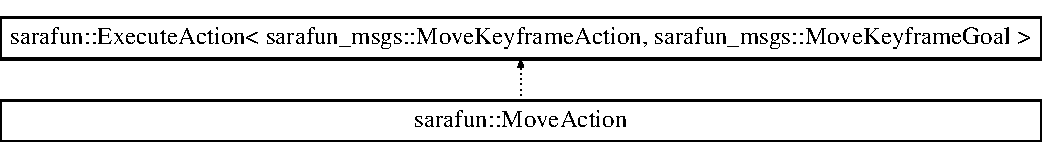
\includegraphics[height=1.914530cm]{classsarafun_1_1MoveAction}
\end{center}
\end{figure}
\subsection*{Public Member Functions}
\begin{DoxyCompactItemize}
\item 
\hyperlink{classsarafun_1_1MoveAction_a423d16aa9d5a47e9f558eae9e013c5e7}{Move\-Action} (std\-::string node\-\_\-name, std\-::string action\-\_\-name, std\-::string bt\-\_\-name)
\item 
\hyperlink{classsarafun_1_1MoveAction_ab9b7f0e483bd9a0b53f9651d661c93b7}{$\sim$\-Move\-Action} ()
\item 
bool \hyperlink{classsarafun_1_1MoveAction_ad5259389b6a5718389c24fab920c9296}{fill\-Goal} (sarafun\-\_\-msgs\-::\-Move\-Keyframe\-Goal \&goal)
\item 
double \hyperlink{classsarafun_1_1MoveAction_a3a0d4d2919b30b878c603a884db6a470}{get\-Timeout\-Value} ()
\end{DoxyCompactItemize}


\subsection{Constructor \& Destructor Documentation}
\hypertarget{classsarafun_1_1MoveAction_a423d16aa9d5a47e9f558eae9e013c5e7}{\index{sarafun\-::\-Move\-Action@{sarafun\-::\-Move\-Action}!Move\-Action@{Move\-Action}}
\index{Move\-Action@{Move\-Action}!sarafun::MoveAction@{sarafun\-::\-Move\-Action}}
\subsubsection[{Move\-Action}]{\setlength{\rightskip}{0pt plus 5cm}sarafun\-::\-Move\-Action\-::\-Move\-Action (
\begin{DoxyParamCaption}
\item[{std\-::string}]{node\-\_\-name, }
\item[{std\-::string}]{action\-\_\-name, }
\item[{std\-::string}]{bt\-\_\-name}
\end{DoxyParamCaption}
)\hspace{0.3cm}{\ttfamily [inline]}}}\label{classsarafun_1_1MoveAction_a423d16aa9d5a47e9f558eae9e013c5e7}
\hypertarget{classsarafun_1_1MoveAction_ab9b7f0e483bd9a0b53f9651d661c93b7}{\index{sarafun\-::\-Move\-Action@{sarafun\-::\-Move\-Action}!$\sim$\-Move\-Action@{$\sim$\-Move\-Action}}
\index{$\sim$\-Move\-Action@{$\sim$\-Move\-Action}!sarafun::MoveAction@{sarafun\-::\-Move\-Action}}
\subsubsection[{$\sim$\-Move\-Action}]{\setlength{\rightskip}{0pt plus 5cm}sarafun\-::\-Move\-Action\-::$\sim$\-Move\-Action (
\begin{DoxyParamCaption}
{}
\end{DoxyParamCaption}
)\hspace{0.3cm}{\ttfamily [inline]}}}\label{classsarafun_1_1MoveAction_ab9b7f0e483bd9a0b53f9651d661c93b7}


\subsection{Member Function Documentation}
\hypertarget{classsarafun_1_1MoveAction_ad5259389b6a5718389c24fab920c9296}{\index{sarafun\-::\-Move\-Action@{sarafun\-::\-Move\-Action}!fill\-Goal@{fill\-Goal}}
\index{fill\-Goal@{fill\-Goal}!sarafun::MoveAction@{sarafun\-::\-Move\-Action}}
\subsubsection[{fill\-Goal}]{\setlength{\rightskip}{0pt plus 5cm}bool sarafun\-::\-Move\-Action\-::fill\-Goal (
\begin{DoxyParamCaption}
\item[{sarafun\-\_\-msgs\-::\-Move\-Keyframe\-Goal \&}]{goal}
\end{DoxyParamCaption}
)\hspace{0.3cm}{\ttfamily [virtual]}}}\label{classsarafun_1_1MoveAction_ad5259389b6a5718389c24fab920c9296}
Fills in the goal for a particular action.


\begin{DoxyParams}{Parameters}
{\em goal} & The actionlib goal message of the externally implemented action. \\
\hline
\end{DoxyParams}
\begin{DoxyReturn}{Returns}
False in case of error, true otherwise. 
\end{DoxyReturn}


Implements \hyperlink{classsarafun_1_1ExecuteAction_a6dd9c0f013d15a17d7e7ce8dbe40a436}{sarafun\-::\-Execute\-Action$<$ sarafun\-\_\-msgs\-::\-Move\-Keyframe\-Action, sarafun\-\_\-msgs\-::\-Move\-Keyframe\-Goal $>$}.

\hypertarget{classsarafun_1_1MoveAction_a3a0d4d2919b30b878c603a884db6a470}{\index{sarafun\-::\-Move\-Action@{sarafun\-::\-Move\-Action}!get\-Timeout\-Value@{get\-Timeout\-Value}}
\index{get\-Timeout\-Value@{get\-Timeout\-Value}!sarafun::MoveAction@{sarafun\-::\-Move\-Action}}
\subsubsection[{get\-Timeout\-Value}]{\setlength{\rightskip}{0pt plus 5cm}double sarafun\-::\-Move\-Action\-::get\-Timeout\-Value (
\begin{DoxyParamCaption}
{}
\end{DoxyParamCaption}
)\hspace{0.3cm}{\ttfamily [virtual]}}}\label{classsarafun_1_1MoveAction_a3a0d4d2919b30b878c603a884db6a470}
Provides the client with a timeout value for actionlib connections.

\begin{DoxyReturn}{Returns}
The timeout value (in seconds). 
\end{DoxyReturn}


Implements \hyperlink{classsarafun_1_1ExecuteAction_aba6cfa8a8ce19e735eb6394424df6d17}{sarafun\-::\-Execute\-Action$<$ sarafun\-\_\-msgs\-::\-Move\-Keyframe\-Action, sarafun\-\_\-msgs\-::\-Move\-Keyframe\-Goal $>$}.



The documentation for this class was generated from the following files\-:\begin{DoxyCompactItemize}
\item 
sarafun\-\_\-tree/include/sarafun\-\_\-tree/sarafun\-\_\-action\-\_\-nodes/\hyperlink{MoveAction_8h}{Move\-Action.\-h}\item 
sarafun\-\_\-tree/src/sarafun\-\_\-action\-\_\-nodes/\hyperlink{MoveAction_8cpp}{Move\-Action.\-cpp}\end{DoxyCompactItemize}

\hypertarget{classsarafun_1_1OnlineMotionAction}{\section{sarafun\-:\-:Online\-Motion\-Action Class Reference}
\label{classsarafun_1_1OnlineMotionAction}\index{sarafun\-::\-Online\-Motion\-Action@{sarafun\-::\-Online\-Motion\-Action}}
}


{\ttfamily \#include $<$Online\-Motion\-Action.\-h$>$}

Inheritance diagram for sarafun\-:\-:Online\-Motion\-Action\-:\begin{figure}[H]
\begin{center}
\leavevmode
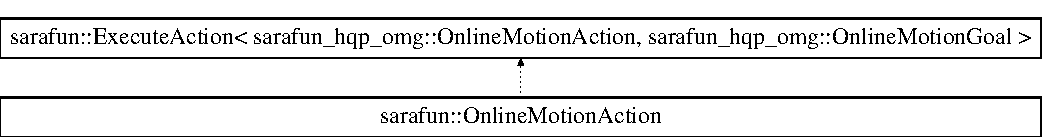
\includegraphics[height=1.845140cm]{classsarafun_1_1OnlineMotionAction}
\end{center}
\end{figure}
\subsection*{Public Member Functions}
\begin{DoxyCompactItemize}
\item 
\hyperlink{classsarafun_1_1OnlineMotionAction_ab66225e6e9383411dc925e88fb1cf4f9}{Online\-Motion\-Action} (std\-::string node\-\_\-name, std\-::string action\-\_\-name, std\-::string bt\-\_\-name)
\item 
\hyperlink{classsarafun_1_1OnlineMotionAction_a63134a65e9ead7a8250abe2afee5b388}{$\sim$\-Online\-Motion\-Action} ()
\item 
bool \hyperlink{classsarafun_1_1OnlineMotionAction_aacaa264dad7ba07b5c9a985d66ea48f7}{fill\-Goal} (sarafun\-\_\-hqp\-\_\-omg\-::\-Online\-Motion\-Goal \&goal)
\item 
double \hyperlink{classsarafun_1_1OnlineMotionAction_a453e7dca41a0d73b5297ce191e760b31}{get\-Timeout\-Value} ()
\end{DoxyCompactItemize}


\subsection{Constructor \& Destructor Documentation}
\hypertarget{classsarafun_1_1OnlineMotionAction_ab66225e6e9383411dc925e88fb1cf4f9}{\index{sarafun\-::\-Online\-Motion\-Action@{sarafun\-::\-Online\-Motion\-Action}!Online\-Motion\-Action@{Online\-Motion\-Action}}
\index{Online\-Motion\-Action@{Online\-Motion\-Action}!sarafun::OnlineMotionAction@{sarafun\-::\-Online\-Motion\-Action}}
\subsubsection[{Online\-Motion\-Action}]{\setlength{\rightskip}{0pt plus 5cm}sarafun\-::\-Online\-Motion\-Action\-::\-Online\-Motion\-Action (
\begin{DoxyParamCaption}
\item[{std\-::string}]{node\-\_\-name, }
\item[{std\-::string}]{action\-\_\-name, }
\item[{std\-::string}]{bt\-\_\-name}
\end{DoxyParamCaption}
)\hspace{0.3cm}{\ttfamily [inline]}}}\label{classsarafun_1_1OnlineMotionAction_ab66225e6e9383411dc925e88fb1cf4f9}
\hypertarget{classsarafun_1_1OnlineMotionAction_a63134a65e9ead7a8250abe2afee5b388}{\index{sarafun\-::\-Online\-Motion\-Action@{sarafun\-::\-Online\-Motion\-Action}!$\sim$\-Online\-Motion\-Action@{$\sim$\-Online\-Motion\-Action}}
\index{$\sim$\-Online\-Motion\-Action@{$\sim$\-Online\-Motion\-Action}!sarafun::OnlineMotionAction@{sarafun\-::\-Online\-Motion\-Action}}
\subsubsection[{$\sim$\-Online\-Motion\-Action}]{\setlength{\rightskip}{0pt plus 5cm}sarafun\-::\-Online\-Motion\-Action\-::$\sim$\-Online\-Motion\-Action (
\begin{DoxyParamCaption}
{}
\end{DoxyParamCaption}
)\hspace{0.3cm}{\ttfamily [inline]}}}\label{classsarafun_1_1OnlineMotionAction_a63134a65e9ead7a8250abe2afee5b388}


\subsection{Member Function Documentation}
\hypertarget{classsarafun_1_1OnlineMotionAction_aacaa264dad7ba07b5c9a985d66ea48f7}{\index{sarafun\-::\-Online\-Motion\-Action@{sarafun\-::\-Online\-Motion\-Action}!fill\-Goal@{fill\-Goal}}
\index{fill\-Goal@{fill\-Goal}!sarafun::OnlineMotionAction@{sarafun\-::\-Online\-Motion\-Action}}
\subsubsection[{fill\-Goal}]{\setlength{\rightskip}{0pt plus 5cm}bool sarafun\-::\-Online\-Motion\-Action\-::fill\-Goal (
\begin{DoxyParamCaption}
\item[{sarafun\-\_\-hqp\-\_\-omg\-::\-Online\-Motion\-Goal \&}]{goal}
\end{DoxyParamCaption}
)\hspace{0.3cm}{\ttfamily [virtual]}}}\label{classsarafun_1_1OnlineMotionAction_aacaa264dad7ba07b5c9a985d66ea48f7}
Fills in the goal for a particular action.


\begin{DoxyParams}{Parameters}
{\em goal} & The actionlib goal message of the externally implemented action. \\
\hline
\end{DoxyParams}
\begin{DoxyReturn}{Returns}
False in case of error, true otherwise. 
\end{DoxyReturn}


Implements \hyperlink{classsarafun_1_1ExecuteAction_a6dd9c0f013d15a17d7e7ce8dbe40a436}{sarafun\-::\-Execute\-Action$<$ sarafun\-\_\-hqp\-\_\-omg\-::\-Online\-Motion\-Action, sarafun\-\_\-hqp\-\_\-omg\-::\-Online\-Motion\-Goal $>$}.

\hypertarget{classsarafun_1_1OnlineMotionAction_a453e7dca41a0d73b5297ce191e760b31}{\index{sarafun\-::\-Online\-Motion\-Action@{sarafun\-::\-Online\-Motion\-Action}!get\-Timeout\-Value@{get\-Timeout\-Value}}
\index{get\-Timeout\-Value@{get\-Timeout\-Value}!sarafun::OnlineMotionAction@{sarafun\-::\-Online\-Motion\-Action}}
\subsubsection[{get\-Timeout\-Value}]{\setlength{\rightskip}{0pt plus 5cm}double sarafun\-::\-Online\-Motion\-Action\-::get\-Timeout\-Value (
\begin{DoxyParamCaption}
{}
\end{DoxyParamCaption}
)\hspace{0.3cm}{\ttfamily [virtual]}}}\label{classsarafun_1_1OnlineMotionAction_a453e7dca41a0d73b5297ce191e760b31}
Provides the client with a timeout value for actionlib connections.

\begin{DoxyReturn}{Returns}
The timeout value (in seconds). 
\end{DoxyReturn}


Implements \hyperlink{classsarafun_1_1ExecuteAction_aba6cfa8a8ce19e735eb6394424df6d17}{sarafun\-::\-Execute\-Action$<$ sarafun\-\_\-hqp\-\_\-omg\-::\-Online\-Motion\-Action, sarafun\-\_\-hqp\-\_\-omg\-::\-Online\-Motion\-Goal $>$}.



The documentation for this class was generated from the following files\-:\begin{DoxyCompactItemize}
\item 
sarafun\-\_\-tree/include/sarafun\-\_\-tree/demo\-\_\-bt\-\_\-nodes/\hyperlink{OnlineMotionAction_8h}{Online\-Motion\-Action.\-h}\item 
sarafun\-\_\-tree/src/demo\-\_\-bt\-\_\-nodes/\hyperlink{OnlineMotionAction_8cpp}{Online\-Motion\-Action.\-cpp}\end{DoxyCompactItemize}

\hypertarget{classbt__parser_1_1Parser}{\section{bt\-\_\-parser\-:\-:Parser Class Reference}
\label{classbt__parser_1_1Parser}\index{bt\-\_\-parser\-::\-Parser@{bt\-\_\-parser\-::\-Parser}}
}


{\ttfamily \#include $<$parse\-\_\-tree.\-h$>$}



Collaboration diagram for bt\-\_\-parser\-:\-:Parser\-:\nopagebreak
\begin{figure}[H]
\begin{center}
\leavevmode
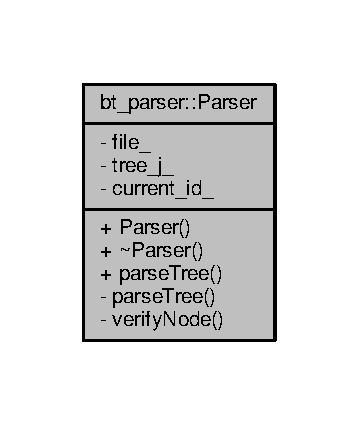
\includegraphics[width=172pt]{d2/d92/classbt__parser_1_1Parser__coll__graph}
\end{center}
\end{figure}
\subsection*{Public Member Functions}
\begin{DoxyCompactItemize}
\item 
\hyperlink{classbt__parser_1_1Parser_abcd6235386f006f36b56ceb08c898deb_abcd6235386f006f36b56ceb08c898deb}{Parser} (std\-::string filepath)
\item 
\hyperlink{classbt__parser_1_1Parser_a5a8992b935e01bac1fa36da4d20eb718_a5a8992b935e01bac1fa36da4d20eb718}{$\sim$\-Parser} ()
\item 
B\-T\-::\-Tree\-Node $\ast$ \hyperlink{classbt__parser_1_1Parser_a7c744cc625df4ce26fbaa3deba496737_a7c744cc625df4ce26fbaa3deba496737}{parse\-Tree} ()
\end{DoxyCompactItemize}
\subsection*{Private Member Functions}
\begin{DoxyCompactItemize}
\item 
B\-T\-::\-Tree\-Node $\ast$ \hyperlink{classbt__parser_1_1Parser_a30c924ebeff1273b8612c41bd5e7ffe2_a30c924ebeff1273b8612c41bd5e7ffe2}{parse\-Tree} (json node)
\item 
void \hyperlink{classbt__parser_1_1Parser_a67d8ea4c25f3088b8e5b18cc01837d1a_a67d8ea4c25f3088b8e5b18cc01837d1a}{verify\-Node} (json node)
\end{DoxyCompactItemize}
\subsection*{Private Attributes}
\begin{DoxyCompactItemize}
\item 
std\-::ifstream \hyperlink{classbt__parser_1_1Parser_a2f2c7b9fcfd823c22b8e4385e8e2ce63_a2f2c7b9fcfd823c22b8e4385e8e2ce63}{file\-\_\-}
\item 
json \hyperlink{classbt__parser_1_1Parser_abd894df8a1d8c0aaf660fc02ca1f3882_abd894df8a1d8c0aaf660fc02ca1f3882}{tree\-\_\-j\-\_\-}
\item 
std\-::string \hyperlink{classbt__parser_1_1Parser_a8a2cd4996ff4cc8a6de26caa52756620_a8a2cd4996ff4cc8a6de26caa52756620}{current\-\_\-id\-\_\-}
\end{DoxyCompactItemize}


\subsection{Detailed Description}
Implements a behavior tree parser, that reads a J\-S\-O\-N file describing the tree and generates the executable tree structure. 

Definition at line 17 of file parse\-\_\-tree.\-h.



\subsection{Constructor \& Destructor Documentation}
\hypertarget{classbt__parser_1_1Parser_abcd6235386f006f36b56ceb08c898deb_abcd6235386f006f36b56ceb08c898deb}{\index{bt\-\_\-parser\-::\-Parser@{bt\-\_\-parser\-::\-Parser}!Parser@{Parser}}
\index{Parser@{Parser}!bt_parser::Parser@{bt\-\_\-parser\-::\-Parser}}
\subsubsection[{Parser}]{\setlength{\rightskip}{0pt plus 5cm}bt\-\_\-parser\-::\-Parser\-::\-Parser (
\begin{DoxyParamCaption}
\item[{std\-::string}]{filepath}
\end{DoxyParamCaption}
)}}\label{classbt__parser_1_1Parser_abcd6235386f006f36b56ceb08c898deb_abcd6235386f006f36b56ceb08c898deb}

\begin{DoxyParams}{Parameters}
{\em filepath} & The directory of the J\-S\-O\-N tree description. \\
\hline
\end{DoxyParams}


Definition at line 5 of file parse\-\_\-tree.\-cpp.



References file\-\_\-.

\hypertarget{classbt__parser_1_1Parser_a5a8992b935e01bac1fa36da4d20eb718_a5a8992b935e01bac1fa36da4d20eb718}{\index{bt\-\_\-parser\-::\-Parser@{bt\-\_\-parser\-::\-Parser}!$\sim$\-Parser@{$\sim$\-Parser}}
\index{$\sim$\-Parser@{$\sim$\-Parser}!bt_parser::Parser@{bt\-\_\-parser\-::\-Parser}}
\subsubsection[{$\sim$\-Parser}]{\setlength{\rightskip}{0pt plus 5cm}bt\-\_\-parser\-::\-Parser\-::$\sim$\-Parser (
\begin{DoxyParamCaption}
{}
\end{DoxyParamCaption}
)}}\label{classbt__parser_1_1Parser_a5a8992b935e01bac1fa36da4d20eb718_a5a8992b935e01bac1fa36da4d20eb718}


Definition at line 6 of file parse\-\_\-tree.\-cpp.



References file\-\_\-.



\subsection{Member Function Documentation}
\hypertarget{classbt__parser_1_1Parser_a7c744cc625df4ce26fbaa3deba496737_a7c744cc625df4ce26fbaa3deba496737}{\index{bt\-\_\-parser\-::\-Parser@{bt\-\_\-parser\-::\-Parser}!parse\-Tree@{parse\-Tree}}
\index{parse\-Tree@{parse\-Tree}!bt_parser::Parser@{bt\-\_\-parser\-::\-Parser}}
\subsubsection[{parse\-Tree}]{\setlength{\rightskip}{0pt plus 5cm}B\-T\-::\-Tree\-Node $\ast$ bt\-\_\-parser\-::\-Parser\-::parse\-Tree (
\begin{DoxyParamCaption}
{}
\end{DoxyParamCaption}
)}}\label{classbt__parser_1_1Parser_a7c744cc625df4ce26fbaa3deba496737_a7c744cc625df4ce26fbaa3deba496737}


Definition at line 29 of file parse\-\_\-tree.\-cpp.



References current\-\_\-id\-\_\-, file\-\_\-, and tree\-\_\-j\-\_\-.



Referenced by parse\-Tree().

\hypertarget{classbt__parser_1_1Parser_a30c924ebeff1273b8612c41bd5e7ffe2_a30c924ebeff1273b8612c41bd5e7ffe2}{\index{bt\-\_\-parser\-::\-Parser@{bt\-\_\-parser\-::\-Parser}!parse\-Tree@{parse\-Tree}}
\index{parse\-Tree@{parse\-Tree}!bt_parser::Parser@{bt\-\_\-parser\-::\-Parser}}
\subsubsection[{parse\-Tree}]{\setlength{\rightskip}{0pt plus 5cm}B\-T\-::\-Tree\-Node $\ast$ bt\-\_\-parser\-::\-Parser\-::parse\-Tree (
\begin{DoxyParamCaption}
\item[{json}]{node}
\end{DoxyParamCaption}
)\hspace{0.3cm}{\ttfamily [private]}}}\label{classbt__parser_1_1Parser_a30c924ebeff1273b8612c41bd5e7ffe2_a30c924ebeff1273b8612c41bd5e7ffe2}


Definition at line 56 of file parse\-\_\-tree.\-cpp.



References current\-\_\-id\-\_\-, parse\-Tree(), tree\-\_\-j\-\_\-, and verify\-Node().



Here is the call graph for this function\-:\nopagebreak
\begin{figure}[H]
\begin{center}
\leavevmode
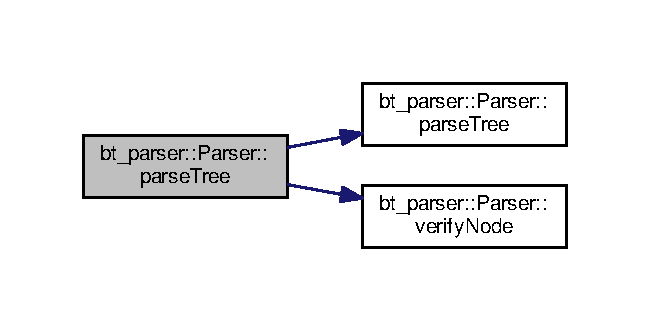
\includegraphics[width=312pt]{dd/d2f/classbt__parser_1_1Parser_a30c924ebeff1273b8612c41bd5e7ffe2_a30c924ebeff1273b8612c41bd5e7ffe2_cgraph}
\end{center}
\end{figure}


\hypertarget{classbt__parser_1_1Parser_a67d8ea4c25f3088b8e5b18cc01837d1a_a67d8ea4c25f3088b8e5b18cc01837d1a}{\index{bt\-\_\-parser\-::\-Parser@{bt\-\_\-parser\-::\-Parser}!verify\-Node@{verify\-Node}}
\index{verify\-Node@{verify\-Node}!bt_parser::Parser@{bt\-\_\-parser\-::\-Parser}}
\subsubsection[{verify\-Node}]{\setlength{\rightskip}{0pt plus 5cm}void bt\-\_\-parser\-::\-Parser\-::verify\-Node (
\begin{DoxyParamCaption}
\item[{json}]{node}
\end{DoxyParamCaption}
)\hspace{0.3cm}{\ttfamily [private]}}}\label{classbt__parser_1_1Parser_a67d8ea4c25f3088b8e5b18cc01837d1a_a67d8ea4c25f3088b8e5b18cc01837d1a}
Verifies the sanity of the given J\-S\-O\-N node describing a B\-T subtree.


\begin{DoxyParams}{Parameters}
{\em node} & A json node object with a B\-T subtree. \\
\hline
\end{DoxyParams}

\begin{DoxyExceptions}{Exceptions}
{\em logic\-\_\-error} & \\
\hline
\end{DoxyExceptions}


Definition at line 8 of file parse\-\_\-tree.\-cpp.



Referenced by parse\-Tree().



\subsection{Field Documentation}
\hypertarget{classbt__parser_1_1Parser_a8a2cd4996ff4cc8a6de26caa52756620_a8a2cd4996ff4cc8a6de26caa52756620}{\index{bt\-\_\-parser\-::\-Parser@{bt\-\_\-parser\-::\-Parser}!current\-\_\-id\-\_\-@{current\-\_\-id\-\_\-}}
\index{current\-\_\-id\-\_\-@{current\-\_\-id\-\_\-}!bt_parser::Parser@{bt\-\_\-parser\-::\-Parser}}
\subsubsection[{current\-\_\-id\-\_\-}]{\setlength{\rightskip}{0pt plus 5cm}std\-::string bt\-\_\-parser\-::\-Parser\-::current\-\_\-id\-\_\-\hspace{0.3cm}{\ttfamily [private]}}}\label{classbt__parser_1_1Parser_a8a2cd4996ff4cc8a6de26caa52756620_a8a2cd4996ff4cc8a6de26caa52756620}


Definition at line 36 of file parse\-\_\-tree.\-h.



Referenced by parse\-Tree().

\hypertarget{classbt__parser_1_1Parser_a2f2c7b9fcfd823c22b8e4385e8e2ce63_a2f2c7b9fcfd823c22b8e4385e8e2ce63}{\index{bt\-\_\-parser\-::\-Parser@{bt\-\_\-parser\-::\-Parser}!file\-\_\-@{file\-\_\-}}
\index{file\-\_\-@{file\-\_\-}!bt_parser::Parser@{bt\-\_\-parser\-::\-Parser}}
\subsubsection[{file\-\_\-}]{\setlength{\rightskip}{0pt plus 5cm}std\-::ifstream bt\-\_\-parser\-::\-Parser\-::file\-\_\-\hspace{0.3cm}{\ttfamily [private]}}}\label{classbt__parser_1_1Parser_a2f2c7b9fcfd823c22b8e4385e8e2ce63_a2f2c7b9fcfd823c22b8e4385e8e2ce63}


Definition at line 34 of file parse\-\_\-tree.\-h.



Referenced by Parser(), parse\-Tree(), and $\sim$\-Parser().

\hypertarget{classbt__parser_1_1Parser_abd894df8a1d8c0aaf660fc02ca1f3882_abd894df8a1d8c0aaf660fc02ca1f3882}{\index{bt\-\_\-parser\-::\-Parser@{bt\-\_\-parser\-::\-Parser}!tree\-\_\-j\-\_\-@{tree\-\_\-j\-\_\-}}
\index{tree\-\_\-j\-\_\-@{tree\-\_\-j\-\_\-}!bt_parser::Parser@{bt\-\_\-parser\-::\-Parser}}
\subsubsection[{tree\-\_\-j\-\_\-}]{\setlength{\rightskip}{0pt plus 5cm}json bt\-\_\-parser\-::\-Parser\-::tree\-\_\-j\-\_\-\hspace{0.3cm}{\ttfamily [private]}}}\label{classbt__parser_1_1Parser_abd894df8a1d8c0aaf660fc02ca1f3882_abd894df8a1d8c0aaf660fc02ca1f3882}


Definition at line 35 of file parse\-\_\-tree.\-h.



Referenced by parse\-Tree().



The documentation for this class was generated from the following files\-:\begin{DoxyCompactItemize}
\item 
parse\-\_\-tree.\-h\item 
parse\-\_\-tree.\-cpp\end{DoxyCompactItemize}

\hypertarget{classsarafun_1_1PickupAction}{\section{sarafun\-:\-:Pickup\-Action Class Reference}
\label{classsarafun_1_1PickupAction}\index{sarafun\-::\-Pickup\-Action@{sarafun\-::\-Pickup\-Action}}
}


{\ttfamily \#include $<$Pickup\-Action.\-h$>$}



Inheritance diagram for sarafun\-:\-:Pickup\-Action\-:
\nopagebreak
\begin{figure}[H]
\begin{center}
\leavevmode
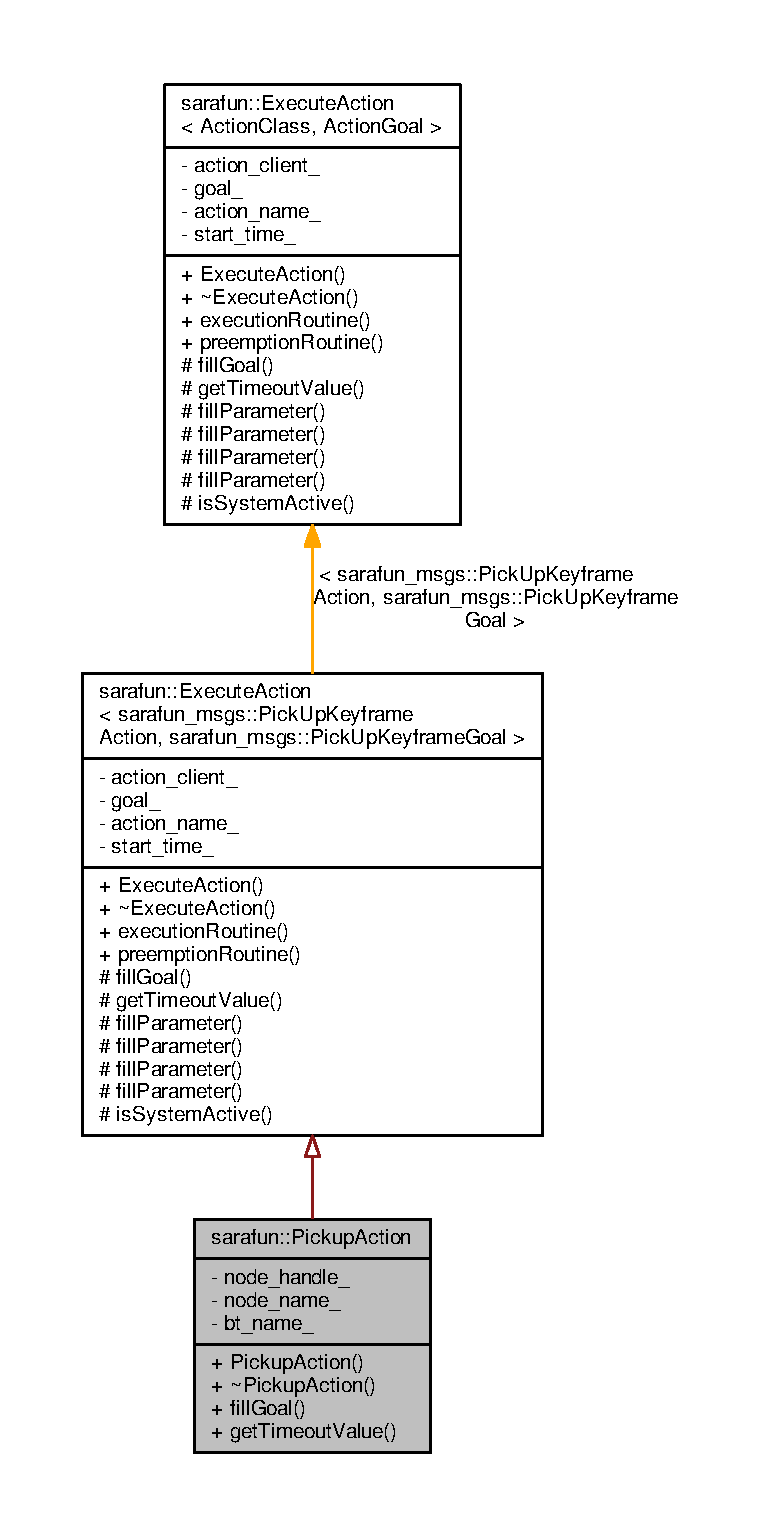
\includegraphics[height=550pt]{db/de1/classsarafun_1_1PickupAction__inherit__graph}
\end{center}
\end{figure}


Collaboration diagram for sarafun\-:\-:Pickup\-Action\-:
\nopagebreak
\begin{figure}[H]
\begin{center}
\leavevmode
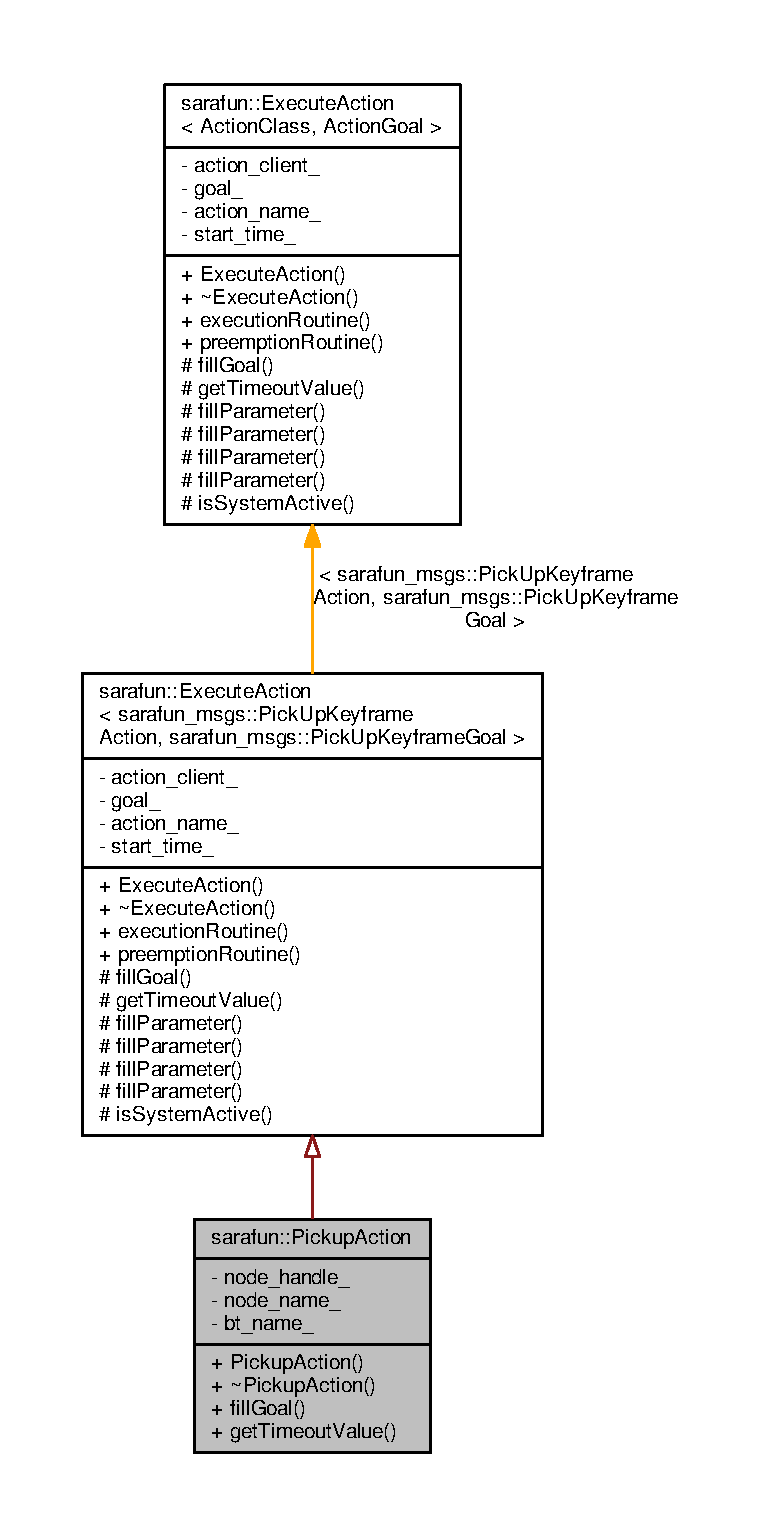
\includegraphics[height=550pt]{d5/da2/classsarafun_1_1PickupAction__coll__graph}
\end{center}
\end{figure}
\subsection*{Public Member Functions}
\begin{DoxyCompactItemize}
\item 
\hyperlink{classsarafun_1_1PickupAction_a1663ebd551413acbc5f21e86a0e3b8cc_a1663ebd551413acbc5f21e86a0e3b8cc}{Pickup\-Action} (std\-::string node\-\_\-name, std\-::string action\-\_\-name, std\-::string bt\-\_\-name)
\item 
\hyperlink{classsarafun_1_1PickupAction_acadfc84a0339caa9cc02c5d599e6aaeb_acadfc84a0339caa9cc02c5d599e6aaeb}{$\sim$\-Pickup\-Action} ()
\item 
bool \hyperlink{classsarafun_1_1PickupAction_a4aa9956733de9f12b52aa41038dbe87a_a4aa9956733de9f12b52aa41038dbe87a}{fill\-Goal} (sarafun\-\_\-msgs\-::\-Pick\-Up\-Keyframe\-Goal \&goal)
\item 
double \hyperlink{classsarafun_1_1PickupAction_a02643cdc836095102e5622b660233f26_a02643cdc836095102e5622b660233f26}{get\-Timeout\-Value} ()
\end{DoxyCompactItemize}
\subsection*{Private Attributes}
\begin{DoxyCompactItemize}
\item 
ros\-::\-Node\-Handle \hyperlink{classsarafun_1_1PickupAction_a7e7ccf1fed497576aebe7bb3c6cb57b3_a7e7ccf1fed497576aebe7bb3c6cb57b3}{node\-\_\-handle\-\_\-}
\item 
std\-::string \hyperlink{classsarafun_1_1PickupAction_a07fa3609628d2c5ac95a6cce904aa1b2_a07fa3609628d2c5ac95a6cce904aa1b2}{node\-\_\-name\-\_\-}
\item 
std\-::string \hyperlink{classsarafun_1_1PickupAction_a67b2fdfacb038bcd76dca5a3c2c2077c_a67b2fdfacb038bcd76dca5a3c2c2077c}{bt\-\_\-name\-\_\-}
\end{DoxyCompactItemize}
\subsection*{Additional Inherited Members}


\subsection{Detailed Description}


Definition at line 9 of file Pickup\-Action.\-h.



\subsection{Constructor \& Destructor Documentation}
\hypertarget{classsarafun_1_1PickupAction_a1663ebd551413acbc5f21e86a0e3b8cc_a1663ebd551413acbc5f21e86a0e3b8cc}{\index{sarafun\-::\-Pickup\-Action@{sarafun\-::\-Pickup\-Action}!Pickup\-Action@{Pickup\-Action}}
\index{Pickup\-Action@{Pickup\-Action}!sarafun::PickupAction@{sarafun\-::\-Pickup\-Action}}
\subsubsection[{Pickup\-Action}]{\setlength{\rightskip}{0pt plus 5cm}sarafun\-::\-Pickup\-Action\-::\-Pickup\-Action (
\begin{DoxyParamCaption}
\item[{std\-::string}]{node\-\_\-name, }
\item[{std\-::string}]{action\-\_\-name, }
\item[{std\-::string}]{bt\-\_\-name}
\end{DoxyParamCaption}
)\hspace{0.3cm}{\ttfamily [inline]}}}\label{classsarafun_1_1PickupAction_a1663ebd551413acbc5f21e86a0e3b8cc_a1663ebd551413acbc5f21e86a0e3b8cc}


Definition at line 13 of file Pickup\-Action.\-h.



References node\-\_\-handle\-\_\-.

\hypertarget{classsarafun_1_1PickupAction_acadfc84a0339caa9cc02c5d599e6aaeb_acadfc84a0339caa9cc02c5d599e6aaeb}{\index{sarafun\-::\-Pickup\-Action@{sarafun\-::\-Pickup\-Action}!$\sim$\-Pickup\-Action@{$\sim$\-Pickup\-Action}}
\index{$\sim$\-Pickup\-Action@{$\sim$\-Pickup\-Action}!sarafun::PickupAction@{sarafun\-::\-Pickup\-Action}}
\subsubsection[{$\sim$\-Pickup\-Action}]{\setlength{\rightskip}{0pt plus 5cm}sarafun\-::\-Pickup\-Action\-::$\sim$\-Pickup\-Action (
\begin{DoxyParamCaption}
{}
\end{DoxyParamCaption}
)\hspace{0.3cm}{\ttfamily [inline]}}}\label{classsarafun_1_1PickupAction_acadfc84a0339caa9cc02c5d599e6aaeb_acadfc84a0339caa9cc02c5d599e6aaeb}


Definition at line 23 of file Pickup\-Action.\-h.



\subsection{Member Function Documentation}
\hypertarget{classsarafun_1_1PickupAction_a4aa9956733de9f12b52aa41038dbe87a_a4aa9956733de9f12b52aa41038dbe87a}{\index{sarafun\-::\-Pickup\-Action@{sarafun\-::\-Pickup\-Action}!fill\-Goal@{fill\-Goal}}
\index{fill\-Goal@{fill\-Goal}!sarafun::PickupAction@{sarafun\-::\-Pickup\-Action}}
\subsubsection[{fill\-Goal}]{\setlength{\rightskip}{0pt plus 5cm}bool sarafun\-::\-Pickup\-Action\-::fill\-Goal (
\begin{DoxyParamCaption}
\item[{sarafun\-\_\-msgs\-::\-Pick\-Up\-Keyframe\-Goal \&}]{goal}
\end{DoxyParamCaption}
)\hspace{0.3cm}{\ttfamily [virtual]}}}\label{classsarafun_1_1PickupAction_a4aa9956733de9f12b52aa41038dbe87a_a4aa9956733de9f12b52aa41038dbe87a}
Fills in the goal for a particular action.


\begin{DoxyParams}{Parameters}
{\em goal} & The actionlib goal message of the externally implemented action. \\
\hline
\end{DoxyParams}
\begin{DoxyReturn}{Returns}
False in case of error, true otherwise. 
\end{DoxyReturn}


Implements \hyperlink{classsarafun_1_1ExecuteAction_a6dd9c0f013d15a17d7e7ce8dbe40a436_a6dd9c0f013d15a17d7e7ce8dbe40a436}{sarafun\-::\-Execute\-Action$<$ sarafun\-\_\-msgs\-::\-Pick\-Up\-Keyframe\-Action, sarafun\-\_\-msgs\-::\-Pick\-Up\-Keyframe\-Goal $>$}.



Definition at line 4 of file Pickup\-Action.\-cpp.



References sarafun\-::\-Execute\-Action$<$ sarafun\-\_\-msgs\-::\-Pick\-Up\-Keyframe\-Action, sarafun\-\_\-msgs\-::\-Pick\-Up\-Keyframe\-Goal $>$\-::fill\-Parameter().



Here is the call graph for this function\-:
\nopagebreak
\begin{figure}[H]
\begin{center}
\leavevmode
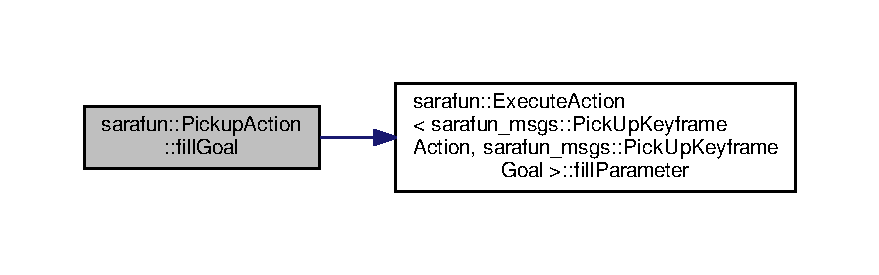
\includegraphics[width=350pt]{d8/dba/classsarafun_1_1PickupAction_a4aa9956733de9f12b52aa41038dbe87a_a4aa9956733de9f12b52aa41038dbe87a_cgraph}
\end{center}
\end{figure}


\hypertarget{classsarafun_1_1PickupAction_a02643cdc836095102e5622b660233f26_a02643cdc836095102e5622b660233f26}{\index{sarafun\-::\-Pickup\-Action@{sarafun\-::\-Pickup\-Action}!get\-Timeout\-Value@{get\-Timeout\-Value}}
\index{get\-Timeout\-Value@{get\-Timeout\-Value}!sarafun::PickupAction@{sarafun\-::\-Pickup\-Action}}
\subsubsection[{get\-Timeout\-Value}]{\setlength{\rightskip}{0pt plus 5cm}double sarafun\-::\-Pickup\-Action\-::get\-Timeout\-Value (
\begin{DoxyParamCaption}
{}
\end{DoxyParamCaption}
)\hspace{0.3cm}{\ttfamily [virtual]}}}\label{classsarafun_1_1PickupAction_a02643cdc836095102e5622b660233f26_a02643cdc836095102e5622b660233f26}
Provides the client with a timeout value for actionlib connections.

\begin{DoxyReturn}{Returns}
The timeout value (in seconds). 
\end{DoxyReturn}


Implements \hyperlink{classsarafun_1_1ExecuteAction_aba6cfa8a8ce19e735eb6394424df6d17_aba6cfa8a8ce19e735eb6394424df6d17}{sarafun\-::\-Execute\-Action$<$ sarafun\-\_\-msgs\-::\-Pick\-Up\-Keyframe\-Action, sarafun\-\_\-msgs\-::\-Pick\-Up\-Keyframe\-Goal $>$}.



Definition at line 13 of file Pickup\-Action.\-cpp.



References sarafun\-::\-Execute\-Action$<$ sarafun\-\_\-msgs\-::\-Pick\-Up\-Keyframe\-Action, sarafun\-\_\-msgs\-::\-Pick\-Up\-Keyframe\-Goal $>$\-::fill\-Parameter().



Here is the call graph for this function\-:
\nopagebreak
\begin{figure}[H]
\begin{center}
\leavevmode
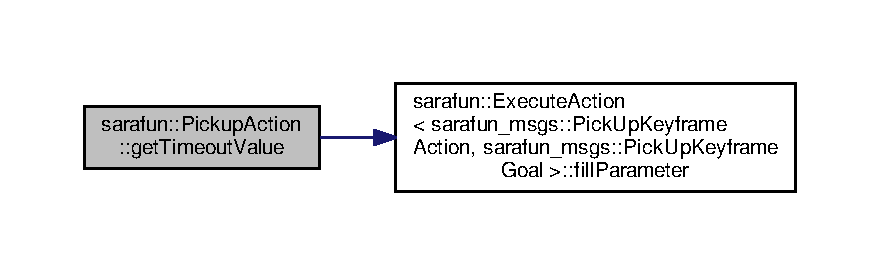
\includegraphics[width=350pt]{d8/dba/classsarafun_1_1PickupAction_a02643cdc836095102e5622b660233f26_a02643cdc836095102e5622b660233f26_cgraph}
\end{center}
\end{figure}




\subsection{Field Documentation}
\hypertarget{classsarafun_1_1PickupAction_a67b2fdfacb038bcd76dca5a3c2c2077c_a67b2fdfacb038bcd76dca5a3c2c2077c}{\index{sarafun\-::\-Pickup\-Action@{sarafun\-::\-Pickup\-Action}!bt\-\_\-name\-\_\-@{bt\-\_\-name\-\_\-}}
\index{bt\-\_\-name\-\_\-@{bt\-\_\-name\-\_\-}!sarafun::PickupAction@{sarafun\-::\-Pickup\-Action}}
\subsubsection[{bt\-\_\-name\-\_\-}]{\setlength{\rightskip}{0pt plus 5cm}std\-::string sarafun\-::\-Pickup\-Action\-::bt\-\_\-name\-\_\-\hspace{0.3cm}{\ttfamily [private]}}}\label{classsarafun_1_1PickupAction_a67b2fdfacb038bcd76dca5a3c2c2077c_a67b2fdfacb038bcd76dca5a3c2c2077c}


Definition at line 31 of file Pickup\-Action.\-h.

\hypertarget{classsarafun_1_1PickupAction_a7e7ccf1fed497576aebe7bb3c6cb57b3_a7e7ccf1fed497576aebe7bb3c6cb57b3}{\index{sarafun\-::\-Pickup\-Action@{sarafun\-::\-Pickup\-Action}!node\-\_\-handle\-\_\-@{node\-\_\-handle\-\_\-}}
\index{node\-\_\-handle\-\_\-@{node\-\_\-handle\-\_\-}!sarafun::PickupAction@{sarafun\-::\-Pickup\-Action}}
\subsubsection[{node\-\_\-handle\-\_\-}]{\setlength{\rightskip}{0pt plus 5cm}ros\-::\-Node\-Handle sarafun\-::\-Pickup\-Action\-::node\-\_\-handle\-\_\-\hspace{0.3cm}{\ttfamily [private]}}}\label{classsarafun_1_1PickupAction_a7e7ccf1fed497576aebe7bb3c6cb57b3_a7e7ccf1fed497576aebe7bb3c6cb57b3}


Definition at line 29 of file Pickup\-Action.\-h.



Referenced by Pickup\-Action().

\hypertarget{classsarafun_1_1PickupAction_a07fa3609628d2c5ac95a6cce904aa1b2_a07fa3609628d2c5ac95a6cce904aa1b2}{\index{sarafun\-::\-Pickup\-Action@{sarafun\-::\-Pickup\-Action}!node\-\_\-name\-\_\-@{node\-\_\-name\-\_\-}}
\index{node\-\_\-name\-\_\-@{node\-\_\-name\-\_\-}!sarafun::PickupAction@{sarafun\-::\-Pickup\-Action}}
\subsubsection[{node\-\_\-name\-\_\-}]{\setlength{\rightskip}{0pt plus 5cm}std\-::string sarafun\-::\-Pickup\-Action\-::node\-\_\-name\-\_\-\hspace{0.3cm}{\ttfamily [private]}}}\label{classsarafun_1_1PickupAction_a07fa3609628d2c5ac95a6cce904aa1b2_a07fa3609628d2c5ac95a6cce904aa1b2}


Definition at line 30 of file Pickup\-Action.\-h.



The documentation for this class was generated from the following files\-:\begin{DoxyCompactItemize}
\item 
Pickup\-Action.\-h\item 
Pickup\-Action.\-cpp\end{DoxyCompactItemize}

\hypertarget{classsarafun_1_1PlaceAction}{\section{sarafun\-:\-:Place\-Action Class Reference}
\label{classsarafun_1_1PlaceAction}\index{sarafun\-::\-Place\-Action@{sarafun\-::\-Place\-Action}}
}


{\ttfamily \#include $<$Place\-Action.\-h$>$}



Inheritance diagram for sarafun\-:\-:Place\-Action\-:
\nopagebreak
\begin{figure}[H]
\begin{center}
\leavevmode
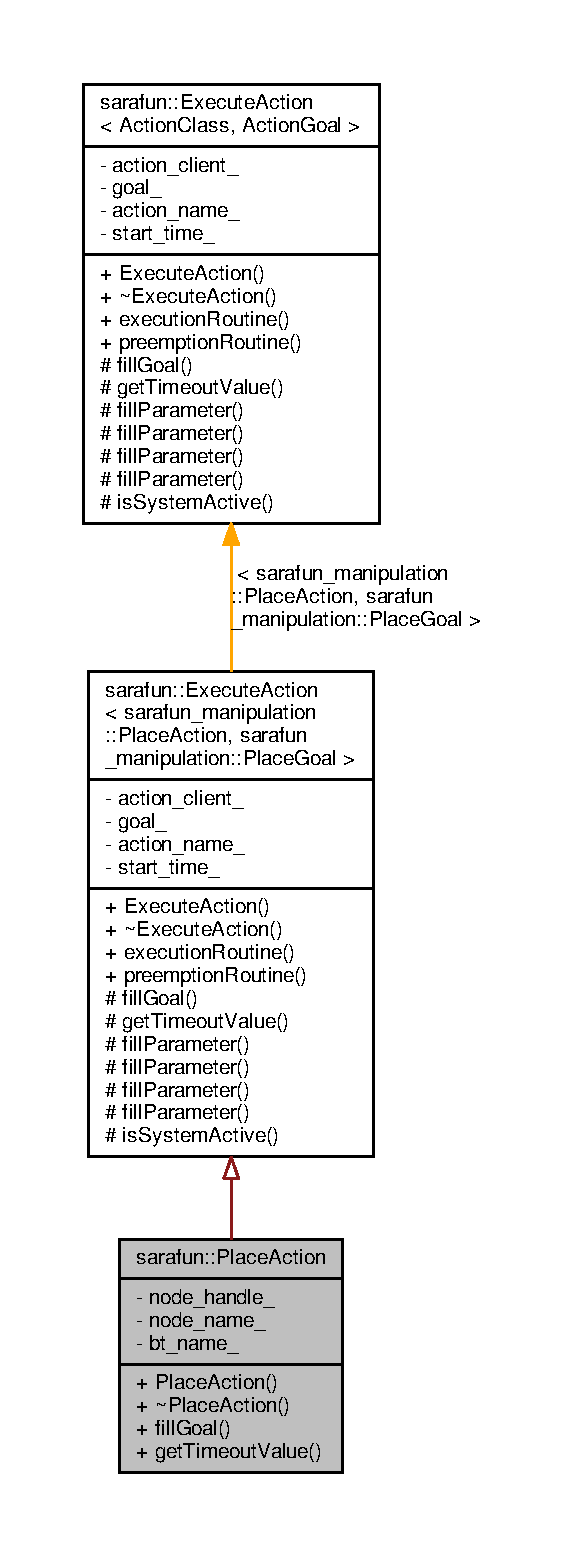
\includegraphics[height=550pt]{dd/d57/classsarafun_1_1PlaceAction__inherit__graph}
\end{center}
\end{figure}


Collaboration diagram for sarafun\-:\-:Place\-Action\-:
\nopagebreak
\begin{figure}[H]
\begin{center}
\leavevmode
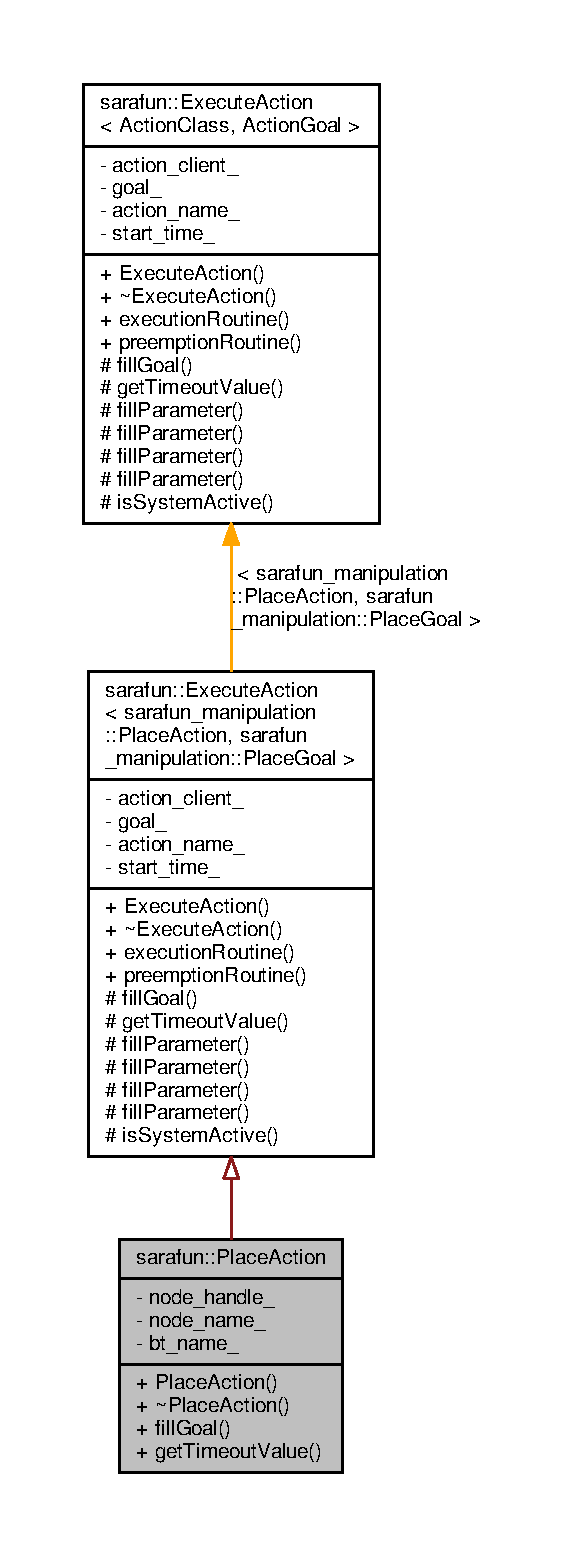
\includegraphics[height=550pt]{d9/df5/classsarafun_1_1PlaceAction__coll__graph}
\end{center}
\end{figure}
\subsection*{Public Member Functions}
\begin{DoxyCompactItemize}
\item 
\hyperlink{classsarafun_1_1PlaceAction_ad55f21266cf4807d831e2834fb6e5259_ad55f21266cf4807d831e2834fb6e5259}{Place\-Action} (std\-::string node\-\_\-name, std\-::string action\-\_\-name, std\-::string bt\-\_\-name)
\item 
\hyperlink{classsarafun_1_1PlaceAction_ae98d86339fdd0d275acff03c968ff834_ae98d86339fdd0d275acff03c968ff834}{$\sim$\-Place\-Action} ()
\item 
bool \hyperlink{classsarafun_1_1PlaceAction_a7d48e758adf6cea93fa15409bafda8c8_a7d48e758adf6cea93fa15409bafda8c8}{fill\-Goal} (sarafun\-\_\-manipulation\-::\-Place\-Goal \&goal)
\item 
double \hyperlink{classsarafun_1_1PlaceAction_a0b53372fd2de920c3ebd94c8c7f80b6a_a0b53372fd2de920c3ebd94c8c7f80b6a}{get\-Timeout\-Value} ()
\end{DoxyCompactItemize}
\subsection*{Private Attributes}
\begin{DoxyCompactItemize}
\item 
ros\-::\-Node\-Handle \hyperlink{classsarafun_1_1PlaceAction_a23f95c7612c9ebb2a64dcfa6ddbd9ec2_a23f95c7612c9ebb2a64dcfa6ddbd9ec2}{node\-\_\-handle\-\_\-}
\item 
std\-::string \hyperlink{classsarafun_1_1PlaceAction_ae8cc4bc053661bae5bdf93a08eaf3416_ae8cc4bc053661bae5bdf93a08eaf3416}{node\-\_\-name\-\_\-}
\item 
std\-::string \hyperlink{classsarafun_1_1PlaceAction_aa477ccd7678ea126e43f3a586be7d72d_aa477ccd7678ea126e43f3a586be7d72d}{bt\-\_\-name\-\_\-}
\end{DoxyCompactItemize}
\subsection*{Additional Inherited Members}


\subsection{Detailed Description}


Definition at line 9 of file Place\-Action.\-h.



\subsection{Constructor \& Destructor Documentation}
\hypertarget{classsarafun_1_1PlaceAction_ad55f21266cf4807d831e2834fb6e5259_ad55f21266cf4807d831e2834fb6e5259}{\index{sarafun\-::\-Place\-Action@{sarafun\-::\-Place\-Action}!Place\-Action@{Place\-Action}}
\index{Place\-Action@{Place\-Action}!sarafun::PlaceAction@{sarafun\-::\-Place\-Action}}
\subsubsection[{Place\-Action}]{\setlength{\rightskip}{0pt plus 5cm}sarafun\-::\-Place\-Action\-::\-Place\-Action (
\begin{DoxyParamCaption}
\item[{std\-::string}]{node\-\_\-name, }
\item[{std\-::string}]{action\-\_\-name, }
\item[{std\-::string}]{bt\-\_\-name}
\end{DoxyParamCaption}
)\hspace{0.3cm}{\ttfamily [inline]}}}\label{classsarafun_1_1PlaceAction_ad55f21266cf4807d831e2834fb6e5259_ad55f21266cf4807d831e2834fb6e5259}


Definition at line 12 of file Place\-Action.\-h.



References node\-\_\-handle\-\_\-.

\hypertarget{classsarafun_1_1PlaceAction_ae98d86339fdd0d275acff03c968ff834_ae98d86339fdd0d275acff03c968ff834}{\index{sarafun\-::\-Place\-Action@{sarafun\-::\-Place\-Action}!$\sim$\-Place\-Action@{$\sim$\-Place\-Action}}
\index{$\sim$\-Place\-Action@{$\sim$\-Place\-Action}!sarafun::PlaceAction@{sarafun\-::\-Place\-Action}}
\subsubsection[{$\sim$\-Place\-Action}]{\setlength{\rightskip}{0pt plus 5cm}sarafun\-::\-Place\-Action\-::$\sim$\-Place\-Action (
\begin{DoxyParamCaption}
{}
\end{DoxyParamCaption}
)\hspace{0.3cm}{\ttfamily [inline]}}}\label{classsarafun_1_1PlaceAction_ae98d86339fdd0d275acff03c968ff834_ae98d86339fdd0d275acff03c968ff834}


Definition at line 22 of file Place\-Action.\-h.



\subsection{Member Function Documentation}
\hypertarget{classsarafun_1_1PlaceAction_a7d48e758adf6cea93fa15409bafda8c8_a7d48e758adf6cea93fa15409bafda8c8}{\index{sarafun\-::\-Place\-Action@{sarafun\-::\-Place\-Action}!fill\-Goal@{fill\-Goal}}
\index{fill\-Goal@{fill\-Goal}!sarafun::PlaceAction@{sarafun\-::\-Place\-Action}}
\subsubsection[{fill\-Goal}]{\setlength{\rightskip}{0pt plus 5cm}bool sarafun\-::\-Place\-Action\-::fill\-Goal (
\begin{DoxyParamCaption}
\item[{sarafun\-\_\-manipulation\-::\-Place\-Goal \&}]{goal}
\end{DoxyParamCaption}
)\hspace{0.3cm}{\ttfamily [virtual]}}}\label{classsarafun_1_1PlaceAction_a7d48e758adf6cea93fa15409bafda8c8_a7d48e758adf6cea93fa15409bafda8c8}
Fills in the goal for a particular action.


\begin{DoxyParams}{Parameters}
{\em goal} & The actionlib goal message of the externally implemented action. \\
\hline
\end{DoxyParams}
\begin{DoxyReturn}{Returns}
False in case of error, true otherwise. 
\end{DoxyReturn}


Implements \hyperlink{classsarafun_1_1ExecuteAction_a6dd9c0f013d15a17d7e7ce8dbe40a436_a6dd9c0f013d15a17d7e7ce8dbe40a436}{sarafun\-::\-Execute\-Action$<$ sarafun\-\_\-manipulation\-::\-Place\-Action, sarafun\-\_\-manipulation\-::\-Place\-Goal $>$}.



Definition at line 11 of file Place\-Action.\-cpp.

\hypertarget{classsarafun_1_1PlaceAction_a0b53372fd2de920c3ebd94c8c7f80b6a_a0b53372fd2de920c3ebd94c8c7f80b6a}{\index{sarafun\-::\-Place\-Action@{sarafun\-::\-Place\-Action}!get\-Timeout\-Value@{get\-Timeout\-Value}}
\index{get\-Timeout\-Value@{get\-Timeout\-Value}!sarafun::PlaceAction@{sarafun\-::\-Place\-Action}}
\subsubsection[{get\-Timeout\-Value}]{\setlength{\rightskip}{0pt plus 5cm}double sarafun\-::\-Place\-Action\-::get\-Timeout\-Value (
\begin{DoxyParamCaption}
{}
\end{DoxyParamCaption}
)\hspace{0.3cm}{\ttfamily [virtual]}}}\label{classsarafun_1_1PlaceAction_a0b53372fd2de920c3ebd94c8c7f80b6a_a0b53372fd2de920c3ebd94c8c7f80b6a}
Provides the client with a timeout value for actionlib connections.

\begin{DoxyReturn}{Returns}
The timeout value (in seconds). 
\end{DoxyReturn}


Implements \hyperlink{classsarafun_1_1ExecuteAction_aba6cfa8a8ce19e735eb6394424df6d17_aba6cfa8a8ce19e735eb6394424df6d17}{sarafun\-::\-Execute\-Action$<$ sarafun\-\_\-manipulation\-::\-Place\-Action, sarafun\-\_\-manipulation\-::\-Place\-Goal $>$}.



Definition at line 4 of file Place\-Action.\-cpp.



References sarafun\-::\-Execute\-Action$<$ sarafun\-\_\-manipulation\-::\-Place\-Action, sarafun\-\_\-manipulation\-::\-Place\-Goal $>$\-::fill\-Parameter().



Here is the call graph for this function\-:
\nopagebreak
\begin{figure}[H]
\begin{center}
\leavevmode
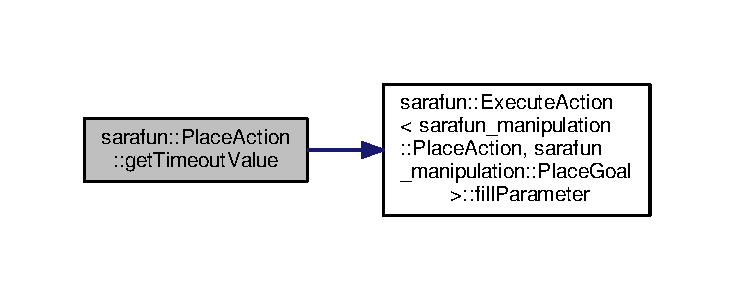
\includegraphics[width=350pt]{d3/dd9/classsarafun_1_1PlaceAction_a0b53372fd2de920c3ebd94c8c7f80b6a_a0b53372fd2de920c3ebd94c8c7f80b6a_cgraph}
\end{center}
\end{figure}




\subsection{Field Documentation}
\hypertarget{classsarafun_1_1PlaceAction_aa477ccd7678ea126e43f3a586be7d72d_aa477ccd7678ea126e43f3a586be7d72d}{\index{sarafun\-::\-Place\-Action@{sarafun\-::\-Place\-Action}!bt\-\_\-name\-\_\-@{bt\-\_\-name\-\_\-}}
\index{bt\-\_\-name\-\_\-@{bt\-\_\-name\-\_\-}!sarafun::PlaceAction@{sarafun\-::\-Place\-Action}}
\subsubsection[{bt\-\_\-name\-\_\-}]{\setlength{\rightskip}{0pt plus 5cm}std\-::string sarafun\-::\-Place\-Action\-::bt\-\_\-name\-\_\-\hspace{0.3cm}{\ttfamily [private]}}}\label{classsarafun_1_1PlaceAction_aa477ccd7678ea126e43f3a586be7d72d_aa477ccd7678ea126e43f3a586be7d72d}


Definition at line 30 of file Place\-Action.\-h.

\hypertarget{classsarafun_1_1PlaceAction_a23f95c7612c9ebb2a64dcfa6ddbd9ec2_a23f95c7612c9ebb2a64dcfa6ddbd9ec2}{\index{sarafun\-::\-Place\-Action@{sarafun\-::\-Place\-Action}!node\-\_\-handle\-\_\-@{node\-\_\-handle\-\_\-}}
\index{node\-\_\-handle\-\_\-@{node\-\_\-handle\-\_\-}!sarafun::PlaceAction@{sarafun\-::\-Place\-Action}}
\subsubsection[{node\-\_\-handle\-\_\-}]{\setlength{\rightskip}{0pt plus 5cm}ros\-::\-Node\-Handle sarafun\-::\-Place\-Action\-::node\-\_\-handle\-\_\-\hspace{0.3cm}{\ttfamily [private]}}}\label{classsarafun_1_1PlaceAction_a23f95c7612c9ebb2a64dcfa6ddbd9ec2_a23f95c7612c9ebb2a64dcfa6ddbd9ec2}


Definition at line 28 of file Place\-Action.\-h.



Referenced by Place\-Action().

\hypertarget{classsarafun_1_1PlaceAction_ae8cc4bc053661bae5bdf93a08eaf3416_ae8cc4bc053661bae5bdf93a08eaf3416}{\index{sarafun\-::\-Place\-Action@{sarafun\-::\-Place\-Action}!node\-\_\-name\-\_\-@{node\-\_\-name\-\_\-}}
\index{node\-\_\-name\-\_\-@{node\-\_\-name\-\_\-}!sarafun::PlaceAction@{sarafun\-::\-Place\-Action}}
\subsubsection[{node\-\_\-name\-\_\-}]{\setlength{\rightskip}{0pt plus 5cm}std\-::string sarafun\-::\-Place\-Action\-::node\-\_\-name\-\_\-\hspace{0.3cm}{\ttfamily [private]}}}\label{classsarafun_1_1PlaceAction_ae8cc4bc053661bae5bdf93a08eaf3416_ae8cc4bc053661bae5bdf93a08eaf3416}


Definition at line 29 of file Place\-Action.\-h.



The documentation for this class was generated from the following files\-:\begin{DoxyCompactItemize}
\item 
Place\-Action.\-h\item 
Place\-Action.\-cpp\end{DoxyCompactItemize}

\hypertarget{classsarafun_1_1RetractAction}{\section{sarafun\-:\-:Retract\-Action Class Reference}
\label{classsarafun_1_1RetractAction}\index{sarafun\-::\-Retract\-Action@{sarafun\-::\-Retract\-Action}}
}


{\ttfamily \#include $<$Retract\-Action.\-h$>$}



Inheritance diagram for sarafun\-:\-:Retract\-Action\-:\nopagebreak
\begin{figure}[H]
\begin{center}
\leavevmode
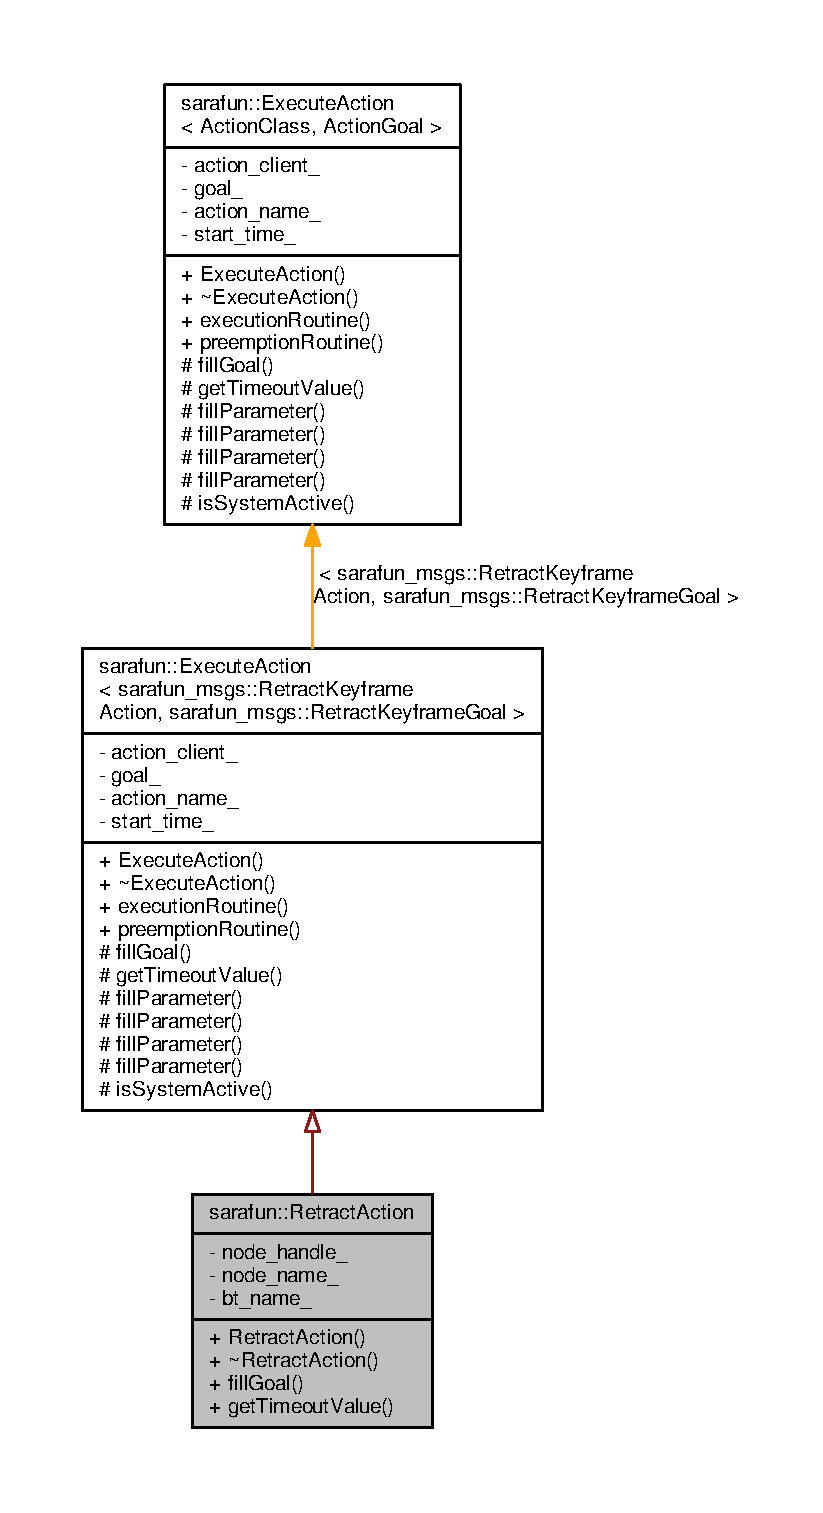
\includegraphics[height=550pt]{d6/d3a/classsarafun_1_1RetractAction__inherit__graph}
\end{center}
\end{figure}


Collaboration diagram for sarafun\-:\-:Retract\-Action\-:\nopagebreak
\begin{figure}[H]
\begin{center}
\leavevmode
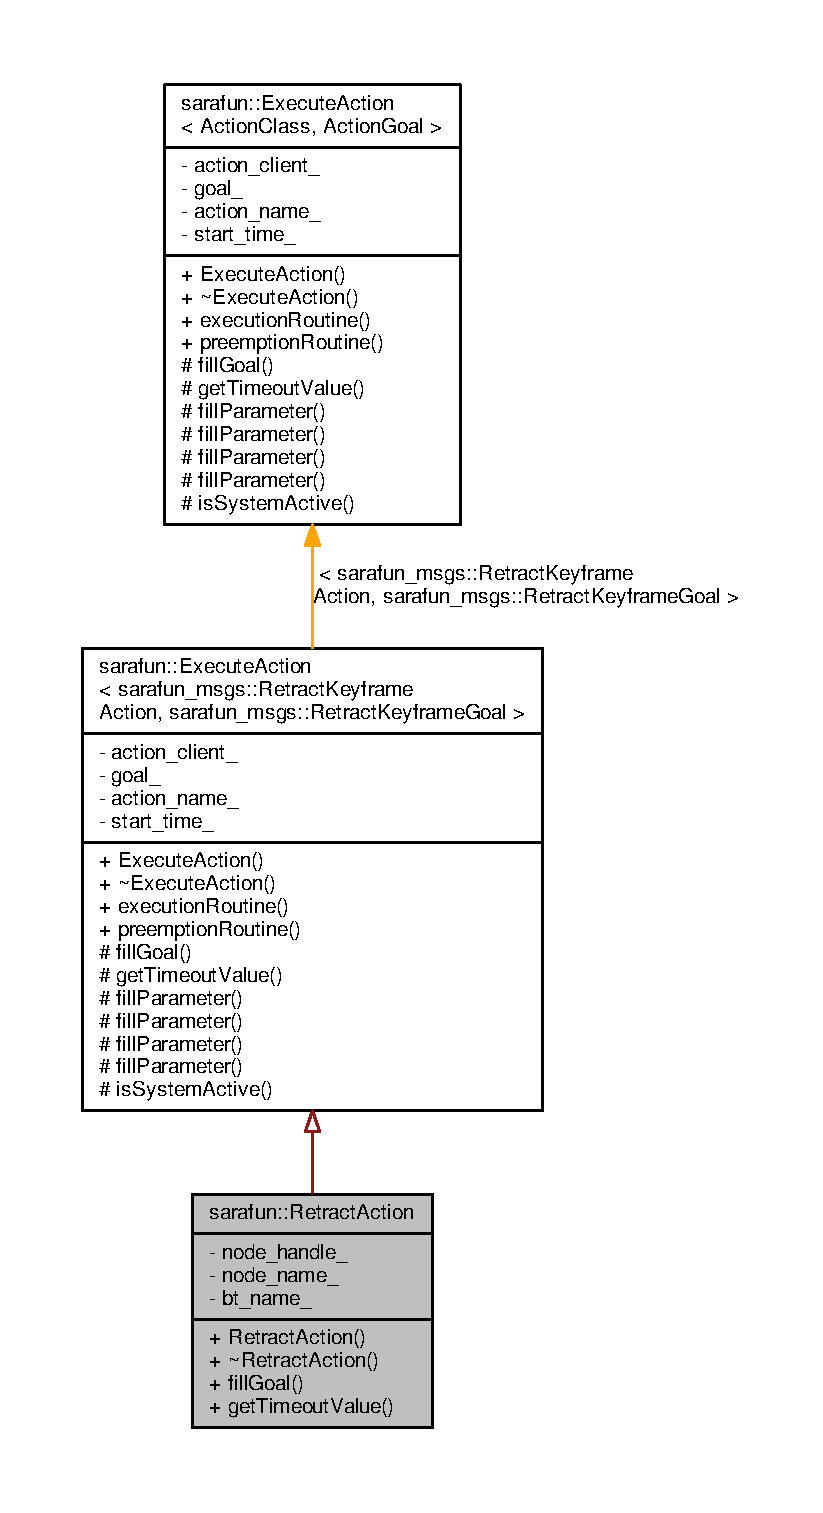
\includegraphics[height=550pt]{de/d4f/classsarafun_1_1RetractAction__coll__graph}
\end{center}
\end{figure}
\subsection*{Public Member Functions}
\begin{DoxyCompactItemize}
\item 
\hyperlink{classsarafun_1_1RetractAction_a0f56a3d5ff6c07f48bbd3cede93f0a81_a0f56a3d5ff6c07f48bbd3cede93f0a81}{Retract\-Action} (std\-::string node\-\_\-name, std\-::string action\-\_\-name, std\-::string bt\-\_\-name)
\item 
\hyperlink{classsarafun_1_1RetractAction_adb37a0fb90d06636009f90b7565f00cf_adb37a0fb90d06636009f90b7565f00cf}{$\sim$\-Retract\-Action} ()
\item 
bool \hyperlink{classsarafun_1_1RetractAction_ad0db1c2615d68603bc972ffa26049a70_ad0db1c2615d68603bc972ffa26049a70}{fill\-Goal} (sarafun\-\_\-msgs\-::\-Retract\-Keyframe\-Goal \&goal)
\item 
double \hyperlink{classsarafun_1_1RetractAction_af95bb8d3826dbe1444a8a3e12d8596b0_af95bb8d3826dbe1444a8a3e12d8596b0}{get\-Timeout\-Value} ()
\end{DoxyCompactItemize}
\subsection*{Private Attributes}
\begin{DoxyCompactItemize}
\item 
ros\-::\-Node\-Handle \hyperlink{classsarafun_1_1RetractAction_aaed00694d79d51ddd40fa3d098faaccd_aaed00694d79d51ddd40fa3d098faaccd}{node\-\_\-handle\-\_\-}
\item 
std\-::string \hyperlink{classsarafun_1_1RetractAction_ab4386c388115f5b76ff82f55895cc1ee_ab4386c388115f5b76ff82f55895cc1ee}{node\-\_\-name\-\_\-}
\item 
std\-::string \hyperlink{classsarafun_1_1RetractAction_a186b48e8f63ea5e0cd8c8047cfa36843_a186b48e8f63ea5e0cd8c8047cfa36843}{bt\-\_\-name\-\_\-}
\end{DoxyCompactItemize}
\subsection*{Additional Inherited Members}


\subsection{Detailed Description}


Definition at line 9 of file Retract\-Action.\-h.



\subsection{Constructor \& Destructor Documentation}
\hypertarget{classsarafun_1_1RetractAction_a0f56a3d5ff6c07f48bbd3cede93f0a81_a0f56a3d5ff6c07f48bbd3cede93f0a81}{\index{sarafun\-::\-Retract\-Action@{sarafun\-::\-Retract\-Action}!Retract\-Action@{Retract\-Action}}
\index{Retract\-Action@{Retract\-Action}!sarafun::RetractAction@{sarafun\-::\-Retract\-Action}}
\subsubsection[{Retract\-Action}]{\setlength{\rightskip}{0pt plus 5cm}sarafun\-::\-Retract\-Action\-::\-Retract\-Action (
\begin{DoxyParamCaption}
\item[{std\-::string}]{node\-\_\-name, }
\item[{std\-::string}]{action\-\_\-name, }
\item[{std\-::string}]{bt\-\_\-name}
\end{DoxyParamCaption}
)\hspace{0.3cm}{\ttfamily [inline]}}}\label{classsarafun_1_1RetractAction_a0f56a3d5ff6c07f48bbd3cede93f0a81_a0f56a3d5ff6c07f48bbd3cede93f0a81}


Definition at line 13 of file Retract\-Action.\-h.



References node\-\_\-handle\-\_\-.

\hypertarget{classsarafun_1_1RetractAction_adb37a0fb90d06636009f90b7565f00cf_adb37a0fb90d06636009f90b7565f00cf}{\index{sarafun\-::\-Retract\-Action@{sarafun\-::\-Retract\-Action}!$\sim$\-Retract\-Action@{$\sim$\-Retract\-Action}}
\index{$\sim$\-Retract\-Action@{$\sim$\-Retract\-Action}!sarafun::RetractAction@{sarafun\-::\-Retract\-Action}}
\subsubsection[{$\sim$\-Retract\-Action}]{\setlength{\rightskip}{0pt plus 5cm}sarafun\-::\-Retract\-Action\-::$\sim$\-Retract\-Action (
\begin{DoxyParamCaption}
{}
\end{DoxyParamCaption}
)\hspace{0.3cm}{\ttfamily [inline]}}}\label{classsarafun_1_1RetractAction_adb37a0fb90d06636009f90b7565f00cf_adb37a0fb90d06636009f90b7565f00cf}


Definition at line 23 of file Retract\-Action.\-h.



\subsection{Member Function Documentation}
\hypertarget{classsarafun_1_1RetractAction_ad0db1c2615d68603bc972ffa26049a70_ad0db1c2615d68603bc972ffa26049a70}{\index{sarafun\-::\-Retract\-Action@{sarafun\-::\-Retract\-Action}!fill\-Goal@{fill\-Goal}}
\index{fill\-Goal@{fill\-Goal}!sarafun::RetractAction@{sarafun\-::\-Retract\-Action}}
\subsubsection[{fill\-Goal}]{\setlength{\rightskip}{0pt plus 5cm}bool sarafun\-::\-Retract\-Action\-::fill\-Goal (
\begin{DoxyParamCaption}
\item[{sarafun\-\_\-msgs\-::\-Retract\-Keyframe\-Goal \&}]{goal}
\end{DoxyParamCaption}
)\hspace{0.3cm}{\ttfamily [virtual]}}}\label{classsarafun_1_1RetractAction_ad0db1c2615d68603bc972ffa26049a70_ad0db1c2615d68603bc972ffa26049a70}
Fills in the goal for a particular action.


\begin{DoxyParams}{Parameters}
{\em goal} & The actionlib goal message of the externally implemented action. \\
\hline
\end{DoxyParams}
\begin{DoxyReturn}{Returns}
False in case of error, true otherwise. 
\end{DoxyReturn}


Implements \hyperlink{classsarafun_1_1ExecuteAction_a6dd9c0f013d15a17d7e7ce8dbe40a436_a6dd9c0f013d15a17d7e7ce8dbe40a436}{sarafun\-::\-Execute\-Action$<$ sarafun\-\_\-msgs\-::\-Retract\-Keyframe\-Action, sarafun\-\_\-msgs\-::\-Retract\-Keyframe\-Goal $>$}.



Definition at line 4 of file Retract\-Action.\-cpp.



References sarafun\-::\-Execute\-Action$<$ sarafun\-\_\-msgs\-::\-Retract\-Keyframe\-Action, sarafun\-\_\-msgs\-::\-Retract\-Keyframe\-Goal $>$\-::fill\-Parameter().



Here is the call graph for this function\-:\nopagebreak
\begin{figure}[H]
\begin{center}
\leavevmode
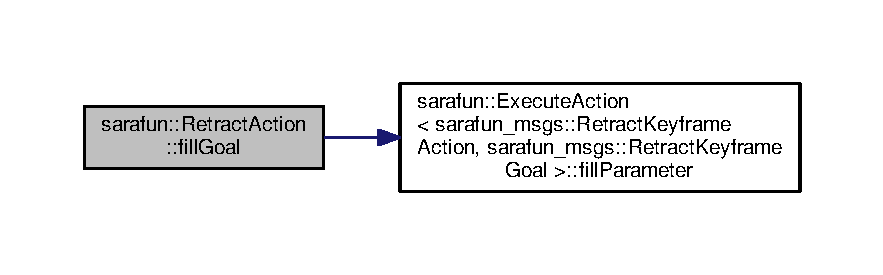
\includegraphics[width=350pt]{d4/dd3/classsarafun_1_1RetractAction_ad0db1c2615d68603bc972ffa26049a70_ad0db1c2615d68603bc972ffa26049a70_cgraph}
\end{center}
\end{figure}


\hypertarget{classsarafun_1_1RetractAction_af95bb8d3826dbe1444a8a3e12d8596b0_af95bb8d3826dbe1444a8a3e12d8596b0}{\index{sarafun\-::\-Retract\-Action@{sarafun\-::\-Retract\-Action}!get\-Timeout\-Value@{get\-Timeout\-Value}}
\index{get\-Timeout\-Value@{get\-Timeout\-Value}!sarafun::RetractAction@{sarafun\-::\-Retract\-Action}}
\subsubsection[{get\-Timeout\-Value}]{\setlength{\rightskip}{0pt plus 5cm}double sarafun\-::\-Retract\-Action\-::get\-Timeout\-Value (
\begin{DoxyParamCaption}
{}
\end{DoxyParamCaption}
)\hspace{0.3cm}{\ttfamily [virtual]}}}\label{classsarafun_1_1RetractAction_af95bb8d3826dbe1444a8a3e12d8596b0_af95bb8d3826dbe1444a8a3e12d8596b0}
Provides the client with a timeout value for actionlib connections.

\begin{DoxyReturn}{Returns}
The timeout value (in seconds). 
\end{DoxyReturn}


Implements \hyperlink{classsarafun_1_1ExecuteAction_aba6cfa8a8ce19e735eb6394424df6d17_aba6cfa8a8ce19e735eb6394424df6d17}{sarafun\-::\-Execute\-Action$<$ sarafun\-\_\-msgs\-::\-Retract\-Keyframe\-Action, sarafun\-\_\-msgs\-::\-Retract\-Keyframe\-Goal $>$}.



Definition at line 13 of file Retract\-Action.\-cpp.



References sarafun\-::\-Execute\-Action$<$ sarafun\-\_\-msgs\-::\-Retract\-Keyframe\-Action, sarafun\-\_\-msgs\-::\-Retract\-Keyframe\-Goal $>$\-::fill\-Parameter().



Here is the call graph for this function\-:\nopagebreak
\begin{figure}[H]
\begin{center}
\leavevmode
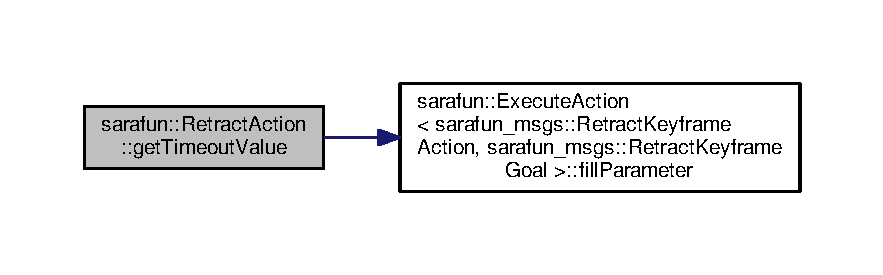
\includegraphics[width=350pt]{d4/dd3/classsarafun_1_1RetractAction_af95bb8d3826dbe1444a8a3e12d8596b0_af95bb8d3826dbe1444a8a3e12d8596b0_cgraph}
\end{center}
\end{figure}




\subsection{Field Documentation}
\hypertarget{classsarafun_1_1RetractAction_a186b48e8f63ea5e0cd8c8047cfa36843_a186b48e8f63ea5e0cd8c8047cfa36843}{\index{sarafun\-::\-Retract\-Action@{sarafun\-::\-Retract\-Action}!bt\-\_\-name\-\_\-@{bt\-\_\-name\-\_\-}}
\index{bt\-\_\-name\-\_\-@{bt\-\_\-name\-\_\-}!sarafun::RetractAction@{sarafun\-::\-Retract\-Action}}
\subsubsection[{bt\-\_\-name\-\_\-}]{\setlength{\rightskip}{0pt plus 5cm}std\-::string sarafun\-::\-Retract\-Action\-::bt\-\_\-name\-\_\-\hspace{0.3cm}{\ttfamily [private]}}}\label{classsarafun_1_1RetractAction_a186b48e8f63ea5e0cd8c8047cfa36843_a186b48e8f63ea5e0cd8c8047cfa36843}


Definition at line 31 of file Retract\-Action.\-h.

\hypertarget{classsarafun_1_1RetractAction_aaed00694d79d51ddd40fa3d098faaccd_aaed00694d79d51ddd40fa3d098faaccd}{\index{sarafun\-::\-Retract\-Action@{sarafun\-::\-Retract\-Action}!node\-\_\-handle\-\_\-@{node\-\_\-handle\-\_\-}}
\index{node\-\_\-handle\-\_\-@{node\-\_\-handle\-\_\-}!sarafun::RetractAction@{sarafun\-::\-Retract\-Action}}
\subsubsection[{node\-\_\-handle\-\_\-}]{\setlength{\rightskip}{0pt plus 5cm}ros\-::\-Node\-Handle sarafun\-::\-Retract\-Action\-::node\-\_\-handle\-\_\-\hspace{0.3cm}{\ttfamily [private]}}}\label{classsarafun_1_1RetractAction_aaed00694d79d51ddd40fa3d098faaccd_aaed00694d79d51ddd40fa3d098faaccd}


Definition at line 29 of file Retract\-Action.\-h.



Referenced by Retract\-Action().

\hypertarget{classsarafun_1_1RetractAction_ab4386c388115f5b76ff82f55895cc1ee_ab4386c388115f5b76ff82f55895cc1ee}{\index{sarafun\-::\-Retract\-Action@{sarafun\-::\-Retract\-Action}!node\-\_\-name\-\_\-@{node\-\_\-name\-\_\-}}
\index{node\-\_\-name\-\_\-@{node\-\_\-name\-\_\-}!sarafun::RetractAction@{sarafun\-::\-Retract\-Action}}
\subsubsection[{node\-\_\-name\-\_\-}]{\setlength{\rightskip}{0pt plus 5cm}std\-::string sarafun\-::\-Retract\-Action\-::node\-\_\-name\-\_\-\hspace{0.3cm}{\ttfamily [private]}}}\label{classsarafun_1_1RetractAction_ab4386c388115f5b76ff82f55895cc1ee_ab4386c388115f5b76ff82f55895cc1ee}


Definition at line 30 of file Retract\-Action.\-h.



The documentation for this class was generated from the following files\-:\begin{DoxyCompactItemize}
\item 
Retract\-Action.\-h\item 
Retract\-Action.\-cpp\end{DoxyCompactItemize}

\hypertarget{classtree__generator_1_1SubTreeFromKF}{\section{tree\-\_\-generator\-:\-:Sub\-Tree\-From\-K\-F Class Reference}
\label{classtree__generator_1_1SubTreeFromKF}\index{tree\-\_\-generator\-::\-Sub\-Tree\-From\-K\-F@{tree\-\_\-generator\-::\-Sub\-Tree\-From\-K\-F}}
}


{\ttfamily \#include $<$Tree\-From\-K\-F.\-hpp$>$}



Collaboration diagram for tree\-\_\-generator\-:\-:Sub\-Tree\-From\-K\-F\-:
\nopagebreak
\begin{figure}[H]
\begin{center}
\leavevmode
\includegraphics[width=236pt]{de/d5a/classtree__generator_1_1SubTreeFromKF__coll__graph}
\end{center}
\end{figure}
\subsection*{Public Member Functions}
\begin{DoxyCompactItemize}
\item 
\hyperlink{classtree__generator_1_1SubTreeFromKF_ab7af1f33766b79ffb8d596db12a567f4_ab7af1f33766b79ffb8d596db12a567f4}{Sub\-Tree\-From\-K\-F} ()
\item 
\hyperlink{classtree__generator_1_1SubTreeFromKF_aa6f44a5c131577ea1719a3fa3a28d65d_aa6f44a5c131577ea1719a3fa3a28d65d}{$\sim$\-Sub\-Tree\-From\-K\-F} ()
\item 
bool \hyperlink{classtree__generator_1_1SubTreeFromKF_a3e4e089333af3305e40434e49dcc0878_a3e4e089333af3305e40434e49dcc0878}{load\-Label} (std\-::string label)
\item 
json \hyperlink{classtree__generator_1_1SubTreeFromKF_a531cc034d2af6a380a40763894542760_a531cc034d2af6a380a40763894542760}{create\-Sub\-Tree} (std\-::vector$<$ int $>$ \&indices)
\end{DoxyCompactItemize}
\subsection*{Private Member Functions}
\begin{DoxyCompactItemize}
\item 
json \hyperlink{classtree__generator_1_1SubTreeFromKF_aea29705cc665f48d15ee436a409d55a9_aea29705cc665f48d15ee436a409d55a9}{modify\-Id} (json node, std\-::vector$<$ int $>$ \&indices)
\end{DoxyCompactItemize}
\subsection*{Private Attributes}
\begin{DoxyCompactItemize}
\item 
ros\-::\-Node\-Handle \hyperlink{classtree__generator_1_1SubTreeFromKF_af32fafef64d1f98df5b38697d1984d80_af32fafef64d1f98df5b38697d1984d80}{nh\-\_\-}
\item 
json \hyperlink{classtree__generator_1_1SubTreeFromKF_a2c9edbe4a6243a1a8bad6ae524df884b_a2c9edbe4a6243a1a8bad6ae524df884b}{subtree\-\_\-}
\item 
std\-::ifstream \hyperlink{classtree__generator_1_1SubTreeFromKF_a66c16669fa438a7a923a88557f8c9654_a66c16669fa438a7a923a88557f8c9654}{file\-\_\-}
\item 
bool \hyperlink{classtree__generator_1_1SubTreeFromKF_abf3280300d7972d36344adf0196d6aba_abf3280300d7972d36344adf0196d6aba}{has\-\_\-label\-\_\-}
\item 
std\-::string \hyperlink{classtree__generator_1_1SubTreeFromKF_a93cab044cd81910fd6b22522e7aa12a6_a93cab044cd81910fd6b22522e7aa12a6}{current\-\_\-id\-\_\-}
\end{DoxyCompactItemize}


\subsection{Detailed Description}
This class constructs one pre-\/defined B\-T subtree, given the semantic information contained in a keyframe.

The files describing the subtrees are defined in the /data/subtrees directory, and must have names matching the labels loaded in the parameter server. 

Definition at line 22 of file Tree\-From\-K\-F.\-hpp.



\subsection{Constructor \& Destructor Documentation}
\hypertarget{classtree__generator_1_1SubTreeFromKF_ab7af1f33766b79ffb8d596db12a567f4_ab7af1f33766b79ffb8d596db12a567f4}{\index{tree\-\_\-generator\-::\-Sub\-Tree\-From\-K\-F@{tree\-\_\-generator\-::\-Sub\-Tree\-From\-K\-F}!Sub\-Tree\-From\-K\-F@{Sub\-Tree\-From\-K\-F}}
\index{Sub\-Tree\-From\-K\-F@{Sub\-Tree\-From\-K\-F}!tree_generator::SubTreeFromKF@{tree\-\_\-generator\-::\-Sub\-Tree\-From\-K\-F}}
\subsubsection[{Sub\-Tree\-From\-K\-F}]{\setlength{\rightskip}{0pt plus 5cm}tree\-\_\-generator\-::\-Sub\-Tree\-From\-K\-F\-::\-Sub\-Tree\-From\-K\-F (
\begin{DoxyParamCaption}
{}
\end{DoxyParamCaption}
)}}\label{classtree__generator_1_1SubTreeFromKF_ab7af1f33766b79ffb8d596db12a567f4_ab7af1f33766b79ffb8d596db12a567f4}


Definition at line 6 of file Tree\-From\-K\-F.\-cpp.



References has\-\_\-label\-\_\-, and nh\-\_\-.

\hypertarget{classtree__generator_1_1SubTreeFromKF_aa6f44a5c131577ea1719a3fa3a28d65d_aa6f44a5c131577ea1719a3fa3a28d65d}{\index{tree\-\_\-generator\-::\-Sub\-Tree\-From\-K\-F@{tree\-\_\-generator\-::\-Sub\-Tree\-From\-K\-F}!$\sim$\-Sub\-Tree\-From\-K\-F@{$\sim$\-Sub\-Tree\-From\-K\-F}}
\index{$\sim$\-Sub\-Tree\-From\-K\-F@{$\sim$\-Sub\-Tree\-From\-K\-F}!tree_generator::SubTreeFromKF@{tree\-\_\-generator\-::\-Sub\-Tree\-From\-K\-F}}
\subsubsection[{$\sim$\-Sub\-Tree\-From\-K\-F}]{\setlength{\rightskip}{0pt plus 5cm}tree\-\_\-generator\-::\-Sub\-Tree\-From\-K\-F\-::$\sim$\-Sub\-Tree\-From\-K\-F (
\begin{DoxyParamCaption}
{}
\end{DoxyParamCaption}
)\hspace{0.3cm}{\ttfamily [inline]}}}\label{classtree__generator_1_1SubTreeFromKF_aa6f44a5c131577ea1719a3fa3a28d65d_aa6f44a5c131577ea1719a3fa3a28d65d}


Definition at line 25 of file Tree\-From\-K\-F.\-hpp.



\subsection{Member Function Documentation}
\hypertarget{classtree__generator_1_1SubTreeFromKF_a531cc034d2af6a380a40763894542760_a531cc034d2af6a380a40763894542760}{\index{tree\-\_\-generator\-::\-Sub\-Tree\-From\-K\-F@{tree\-\_\-generator\-::\-Sub\-Tree\-From\-K\-F}!create\-Sub\-Tree@{create\-Sub\-Tree}}
\index{create\-Sub\-Tree@{create\-Sub\-Tree}!tree_generator::SubTreeFromKF@{tree\-\_\-generator\-::\-Sub\-Tree\-From\-K\-F}}
\subsubsection[{create\-Sub\-Tree}]{\setlength{\rightskip}{0pt plus 5cm}json tree\-\_\-generator\-::\-Sub\-Tree\-From\-K\-F\-::create\-Sub\-Tree (
\begin{DoxyParamCaption}
\item[{std\-::vector$<$ int $>$ \&}]{indices}
\end{DoxyParamCaption}
)}}\label{classtree__generator_1_1SubTreeFromKF_a531cc034d2af6a380a40763894542760_a531cc034d2af6a380a40763894542760}


Definition at line 53 of file Tree\-From\-K\-F.\-cpp.



References file\-\_\-, has\-\_\-label\-\_\-, modify\-Id(), and subtree\-\_\-.



Referenced by tree\-\_\-generator\-::\-Tree\-From\-K\-F\-::create\-Tree().



Here is the call graph for this function\-:
\nopagebreak
\begin{figure}[H]
\begin{center}
\leavevmode
\includegraphics[width=350pt]{d9/de6/classtree__generator_1_1SubTreeFromKF_a531cc034d2af6a380a40763894542760_a531cc034d2af6a380a40763894542760_cgraph}
\end{center}
\end{figure}


\hypertarget{classtree__generator_1_1SubTreeFromKF_a3e4e089333af3305e40434e49dcc0878_a3e4e089333af3305e40434e49dcc0878}{\index{tree\-\_\-generator\-::\-Sub\-Tree\-From\-K\-F@{tree\-\_\-generator\-::\-Sub\-Tree\-From\-K\-F}!load\-Label@{load\-Label}}
\index{load\-Label@{load\-Label}!tree_generator::SubTreeFromKF@{tree\-\_\-generator\-::\-Sub\-Tree\-From\-K\-F}}
\subsubsection[{load\-Label}]{\setlength{\rightskip}{0pt plus 5cm}bool tree\-\_\-generator\-::\-Sub\-Tree\-From\-K\-F\-::load\-Label (
\begin{DoxyParamCaption}
\item[{std\-::string}]{label}
\end{DoxyParamCaption}
)}}\label{classtree__generator_1_1SubTreeFromKF_a3e4e089333af3305e40434e49dcc0878_a3e4e089333af3305e40434e49dcc0878}
Recovers a B\-T subtree with a label that matches the keyframe.


\begin{DoxyParams}{Parameters}
{\em label} & The K\-F label that identifies the subtree. \\
\hline
\end{DoxyParams}
\begin{DoxyReturn}{Returns}
True in case the label exists and the file is recovered. False otherwise. 
\end{DoxyReturn}


Definition at line 26 of file Tree\-From\-K\-F.\-cpp.



References file\-\_\-, has\-\_\-label\-\_\-, nh\-\_\-, and tree\-\_\-generator\-::replace\-With\-Underscore().



Referenced by tree\-\_\-generator\-::\-Tree\-From\-K\-F\-::create\-Tree().



Here is the call graph for this function\-:
\nopagebreak
\begin{figure}[H]
\begin{center}
\leavevmode
\includegraphics[width=350pt]{d9/de6/classtree__generator_1_1SubTreeFromKF_a3e4e089333af3305e40434e49dcc0878_a3e4e089333af3305e40434e49dcc0878_cgraph}
\end{center}
\end{figure}


\hypertarget{classtree__generator_1_1SubTreeFromKF_aea29705cc665f48d15ee436a409d55a9_aea29705cc665f48d15ee436a409d55a9}{\index{tree\-\_\-generator\-::\-Sub\-Tree\-From\-K\-F@{tree\-\_\-generator\-::\-Sub\-Tree\-From\-K\-F}!modify\-Id@{modify\-Id}}
\index{modify\-Id@{modify\-Id}!tree_generator::SubTreeFromKF@{tree\-\_\-generator\-::\-Sub\-Tree\-From\-K\-F}}
\subsubsection[{modify\-Id}]{\setlength{\rightskip}{0pt plus 5cm}json tree\-\_\-generator\-::\-Sub\-Tree\-From\-K\-F\-::modify\-Id (
\begin{DoxyParamCaption}
\item[{json}]{node, }
\item[{std\-::vector$<$ int $>$ \&}]{indices}
\end{DoxyParamCaption}
)\hspace{0.3cm}{\ttfamily [private]}}}\label{classtree__generator_1_1SubTreeFromKF_aea29705cc665f48d15ee436a409d55a9_aea29705cc665f48d15ee436a409d55a9}
Make sure that the created json subtree has nodes with proper indices.


\begin{DoxyParams}{Parameters}
{\em node} & The J\-S\-O\-N node with the subtree description. \\
\hline
{\em indices} & The vector of indices. \\
\hline
\end{DoxyParams}
\begin{DoxyReturn}{Returns}
The modified json N\-O\-D\-E. 
\end{DoxyReturn}

\begin{DoxyExceptions}{Exceptions}
{\em logic\-\_\-error} & \\
\hline
\end{DoxyExceptions}


Definition at line 77 of file Tree\-From\-K\-F.\-cpp.



References tree\-\_\-generator\-::\-A\-C\-T\-I\-O\-N, tree\-\_\-generator\-::\-C\-O\-N\-D\-I\-T\-I\-O\-N, tree\-\_\-generator\-::\-S\-E\-L, tree\-\_\-generator\-::\-S\-E\-L\-S\-T\-A\-R, tree\-\_\-generator\-::\-S\-E\-Q, and tree\-\_\-generator\-::\-S\-E\-Q\-S\-T\-A\-R.



Referenced by create\-Sub\-Tree().



\subsection{Field Documentation}
\hypertarget{classtree__generator_1_1SubTreeFromKF_a93cab044cd81910fd6b22522e7aa12a6_a93cab044cd81910fd6b22522e7aa12a6}{\index{tree\-\_\-generator\-::\-Sub\-Tree\-From\-K\-F@{tree\-\_\-generator\-::\-Sub\-Tree\-From\-K\-F}!current\-\_\-id\-\_\-@{current\-\_\-id\-\_\-}}
\index{current\-\_\-id\-\_\-@{current\-\_\-id\-\_\-}!tree_generator::SubTreeFromKF@{tree\-\_\-generator\-::\-Sub\-Tree\-From\-K\-F}}
\subsubsection[{current\-\_\-id\-\_\-}]{\setlength{\rightskip}{0pt plus 5cm}std\-::string tree\-\_\-generator\-::\-Sub\-Tree\-From\-K\-F\-::current\-\_\-id\-\_\-\hspace{0.3cm}{\ttfamily [private]}}}\label{classtree__generator_1_1SubTreeFromKF_a93cab044cd81910fd6b22522e7aa12a6_a93cab044cd81910fd6b22522e7aa12a6}


Definition at line 52 of file Tree\-From\-K\-F.\-hpp.

\hypertarget{classtree__generator_1_1SubTreeFromKF_a66c16669fa438a7a923a88557f8c9654_a66c16669fa438a7a923a88557f8c9654}{\index{tree\-\_\-generator\-::\-Sub\-Tree\-From\-K\-F@{tree\-\_\-generator\-::\-Sub\-Tree\-From\-K\-F}!file\-\_\-@{file\-\_\-}}
\index{file\-\_\-@{file\-\_\-}!tree_generator::SubTreeFromKF@{tree\-\_\-generator\-::\-Sub\-Tree\-From\-K\-F}}
\subsubsection[{file\-\_\-}]{\setlength{\rightskip}{0pt plus 5cm}std\-::ifstream tree\-\_\-generator\-::\-Sub\-Tree\-From\-K\-F\-::file\-\_\-\hspace{0.3cm}{\ttfamily [private]}}}\label{classtree__generator_1_1SubTreeFromKF_a66c16669fa438a7a923a88557f8c9654_a66c16669fa438a7a923a88557f8c9654}


Definition at line 50 of file Tree\-From\-K\-F.\-hpp.



Referenced by create\-Sub\-Tree(), and load\-Label().

\hypertarget{classtree__generator_1_1SubTreeFromKF_abf3280300d7972d36344adf0196d6aba_abf3280300d7972d36344adf0196d6aba}{\index{tree\-\_\-generator\-::\-Sub\-Tree\-From\-K\-F@{tree\-\_\-generator\-::\-Sub\-Tree\-From\-K\-F}!has\-\_\-label\-\_\-@{has\-\_\-label\-\_\-}}
\index{has\-\_\-label\-\_\-@{has\-\_\-label\-\_\-}!tree_generator::SubTreeFromKF@{tree\-\_\-generator\-::\-Sub\-Tree\-From\-K\-F}}
\subsubsection[{has\-\_\-label\-\_\-}]{\setlength{\rightskip}{0pt plus 5cm}bool tree\-\_\-generator\-::\-Sub\-Tree\-From\-K\-F\-::has\-\_\-label\-\_\-\hspace{0.3cm}{\ttfamily [private]}}}\label{classtree__generator_1_1SubTreeFromKF_abf3280300d7972d36344adf0196d6aba_abf3280300d7972d36344adf0196d6aba}


Definition at line 51 of file Tree\-From\-K\-F.\-hpp.



Referenced by create\-Sub\-Tree(), load\-Label(), and Sub\-Tree\-From\-K\-F().

\hypertarget{classtree__generator_1_1SubTreeFromKF_af32fafef64d1f98df5b38697d1984d80_af32fafef64d1f98df5b38697d1984d80}{\index{tree\-\_\-generator\-::\-Sub\-Tree\-From\-K\-F@{tree\-\_\-generator\-::\-Sub\-Tree\-From\-K\-F}!nh\-\_\-@{nh\-\_\-}}
\index{nh\-\_\-@{nh\-\_\-}!tree_generator::SubTreeFromKF@{tree\-\_\-generator\-::\-Sub\-Tree\-From\-K\-F}}
\subsubsection[{nh\-\_\-}]{\setlength{\rightskip}{0pt plus 5cm}ros\-::\-Node\-Handle tree\-\_\-generator\-::\-Sub\-Tree\-From\-K\-F\-::nh\-\_\-\hspace{0.3cm}{\ttfamily [private]}}}\label{classtree__generator_1_1SubTreeFromKF_af32fafef64d1f98df5b38697d1984d80_af32fafef64d1f98df5b38697d1984d80}


Definition at line 48 of file Tree\-From\-K\-F.\-hpp.



Referenced by load\-Label(), and Sub\-Tree\-From\-K\-F().

\hypertarget{classtree__generator_1_1SubTreeFromKF_a2c9edbe4a6243a1a8bad6ae524df884b_a2c9edbe4a6243a1a8bad6ae524df884b}{\index{tree\-\_\-generator\-::\-Sub\-Tree\-From\-K\-F@{tree\-\_\-generator\-::\-Sub\-Tree\-From\-K\-F}!subtree\-\_\-@{subtree\-\_\-}}
\index{subtree\-\_\-@{subtree\-\_\-}!tree_generator::SubTreeFromKF@{tree\-\_\-generator\-::\-Sub\-Tree\-From\-K\-F}}
\subsubsection[{subtree\-\_\-}]{\setlength{\rightskip}{0pt plus 5cm}json tree\-\_\-generator\-::\-Sub\-Tree\-From\-K\-F\-::subtree\-\_\-\hspace{0.3cm}{\ttfamily [private]}}}\label{classtree__generator_1_1SubTreeFromKF_a2c9edbe4a6243a1a8bad6ae524df884b_a2c9edbe4a6243a1a8bad6ae524df884b}


Definition at line 49 of file Tree\-From\-K\-F.\-hpp.



Referenced by create\-Sub\-Tree().



The documentation for this class was generated from the following files\-:\begin{DoxyCompactItemize}
\item 
Tree\-From\-K\-F.\-hpp\item 
Tree\-From\-K\-F.\-cpp\end{DoxyCompactItemize}

\hypertarget{classsarafun_1_1TestAlign}{\section{sarafun\-:\-:Test\-Align Class Reference}
\label{classsarafun_1_1TestAlign}\index{sarafun\-::\-Test\-Align@{sarafun\-::\-Test\-Align}}
}


{\ttfamily \#include $<$Align\-Dummy.\-h$>$}



Inheritance diagram for sarafun\-:\-:Test\-Align\-:\nopagebreak
\begin{figure}[H]
\begin{center}
\leavevmode
\includegraphics[width=350pt]{df/d5d/classsarafun_1_1TestAlign__inherit__graph}
\end{center}
\end{figure}


Collaboration diagram for sarafun\-:\-:Test\-Align\-:\nopagebreak
\begin{figure}[H]
\begin{center}
\leavevmode
\includegraphics[width=350pt]{d0/d3f/classsarafun_1_1TestAlign__coll__graph}
\end{center}
\end{figure}
\subsection*{Public Member Functions}
\begin{DoxyCompactItemize}
\item 
\hyperlink{classsarafun_1_1TestAlign_aa2815fa88b5bd3f41ba32168d2101d58_aa2815fa88b5bd3f41ba32168d2101d58}{Test\-Align} (std\-::string node\-\_\-name, std\-::string actionlib\-\_\-name)
\item 
\hyperlink{classsarafun_1_1TestAlign_a5d171c40cea90663e8cc6e358132ad3f_a5d171c40cea90663e8cc6e358132ad3f}{$\sim$\-Test\-Align} ()
\end{DoxyCompactItemize}
\subsection*{Protected Member Functions}
\begin{DoxyCompactItemize}
\item 
bool \hyperlink{classsarafun_1_1TestAlign_ac9c8c7df9316690c7f1daf95f9ef7e04_ac9c8c7df9316690c7f1daf95f9ef7e04}{parse\-Goal} (const sarafun\-\_\-msgs\-::\-Align\-Keyframe\-Goal\-Const\-Ptr \&goal)
\end{DoxyCompactItemize}
\subsection*{Additional Inherited Members}


\subsection{Detailed Description}


Definition at line 9 of file Align\-Dummy.\-h.



\subsection{Constructor \& Destructor Documentation}
\hypertarget{classsarafun_1_1TestAlign_aa2815fa88b5bd3f41ba32168d2101d58_aa2815fa88b5bd3f41ba32168d2101d58}{\index{sarafun\-::\-Test\-Align@{sarafun\-::\-Test\-Align}!Test\-Align@{Test\-Align}}
\index{Test\-Align@{Test\-Align}!sarafun::TestAlign@{sarafun\-::\-Test\-Align}}
\subsubsection[{Test\-Align}]{\setlength{\rightskip}{0pt plus 5cm}sarafun\-::\-Test\-Align\-::\-Test\-Align (
\begin{DoxyParamCaption}
\item[{std\-::string}]{node\-\_\-name, }
\item[{std\-::string}]{actionlib\-\_\-name}
\end{DoxyParamCaption}
)\hspace{0.3cm}{\ttfamily [inline]}}}\label{classsarafun_1_1TestAlign_aa2815fa88b5bd3f41ba32168d2101d58_aa2815fa88b5bd3f41ba32168d2101d58}


Definition at line 14 of file Align\-Dummy.\-h.

\hypertarget{classsarafun_1_1TestAlign_a5d171c40cea90663e8cc6e358132ad3f_a5d171c40cea90663e8cc6e358132ad3f}{\index{sarafun\-::\-Test\-Align@{sarafun\-::\-Test\-Align}!$\sim$\-Test\-Align@{$\sim$\-Test\-Align}}
\index{$\sim$\-Test\-Align@{$\sim$\-Test\-Align}!sarafun::TestAlign@{sarafun\-::\-Test\-Align}}
\subsubsection[{$\sim$\-Test\-Align}]{\setlength{\rightskip}{0pt plus 5cm}sarafun\-::\-Test\-Align\-::$\sim$\-Test\-Align (
\begin{DoxyParamCaption}
{}
\end{DoxyParamCaption}
)\hspace{0.3cm}{\ttfamily [inline]}}}\label{classsarafun_1_1TestAlign_a5d171c40cea90663e8cc6e358132ad3f_a5d171c40cea90663e8cc6e358132ad3f}


Definition at line 22 of file Align\-Dummy.\-h.



\subsection{Member Function Documentation}
\hypertarget{classsarafun_1_1TestAlign_ac9c8c7df9316690c7f1daf95f9ef7e04_ac9c8c7df9316690c7f1daf95f9ef7e04}{\index{sarafun\-::\-Test\-Align@{sarafun\-::\-Test\-Align}!parse\-Goal@{parse\-Goal}}
\index{parse\-Goal@{parse\-Goal}!sarafun::TestAlign@{sarafun\-::\-Test\-Align}}
\subsubsection[{parse\-Goal}]{\setlength{\rightskip}{0pt plus 5cm}bool sarafun\-::\-Test\-Align\-::parse\-Goal (
\begin{DoxyParamCaption}
\item[{const sarafun\-\_\-msgs\-::\-Align\-Keyframe\-Goal\-Const\-Ptr \&}]{goal}
\end{DoxyParamCaption}
)\hspace{0.3cm}{\ttfamily [protected]}, {\ttfamily [virtual]}}}\label{classsarafun_1_1TestAlign_ac9c8c7df9316690c7f1daf95f9ef7e04_ac9c8c7df9316690c7f1daf95f9ef7e04}
Should print goal contents on the screen and return true or false depending on if they are properly filled in or not. 

Implements \hyperlink{classsarafun_1_1TestServer_a85b9721105c2a4b46bae26428433513e_a85b9721105c2a4b46bae26428433513e}{sarafun\-::\-Test\-Server$<$ sarafun\-\_\-msgs\-::\-Align\-Keyframe\-Action, sarafun\-\_\-msgs\-::\-Align\-Keyframe\-Goal\-Const\-Ptr, sarafun\-\_\-msgs\-::\-Align\-Keyframe\-Feedback, sarafun\-\_\-msgs\-::\-Align\-Keyframe\-Result $>$}.



Definition at line 4 of file Align\-Dummy.\-cpp.



References sarafun\-::\-Test\-Server$<$ sarafun\-\_\-msgs\-::\-Align\-Keyframe\-Action, sarafun\-\_\-msgs\-::\-Align\-Keyframe\-Goal\-Const\-Ptr, sarafun\-\_\-msgs\-::\-Align\-Keyframe\-Feedback, sarafun\-\_\-msgs\-::\-Align\-Keyframe\-Result $>$\-::action\-\_\-name\-\_\-.



The documentation for this class was generated from the following files\-:\begin{DoxyCompactItemize}
\item 
Align\-Dummy.\-h\item 
Align\-Dummy.\-cpp\end{DoxyCompactItemize}

\hypertarget{classsarafun_1_1TestApproach}{\section{sarafun\-:\-:Test\-Approach Class Reference}
\label{classsarafun_1_1TestApproach}\index{sarafun\-::\-Test\-Approach@{sarafun\-::\-Test\-Approach}}
}


{\ttfamily \#include $<$Approach\-Dummy.\-h$>$}



Inheritance diagram for sarafun\-:\-:Test\-Approach\-:\nopagebreak
\begin{figure}[H]
\begin{center}
\leavevmode
\includegraphics[height=550pt]{d9/d9a/classsarafun_1_1TestApproach__inherit__graph}
\end{center}
\end{figure}


Collaboration diagram for sarafun\-:\-:Test\-Approach\-:\nopagebreak
\begin{figure}[H]
\begin{center}
\leavevmode
\includegraphics[height=550pt]{d1/d01/classsarafun_1_1TestApproach__coll__graph}
\end{center}
\end{figure}
\subsection*{Public Member Functions}
\begin{DoxyCompactItemize}
\item 
\hyperlink{classsarafun_1_1TestApproach_aebd82243594c941ecceb4f73b44d4139_aebd82243594c941ecceb4f73b44d4139}{Test\-Approach} (std\-::string node\-\_\-name, std\-::string actionlib\-\_\-name)
\item 
\hyperlink{classsarafun_1_1TestApproach_a5a261f65818ad6ee669b75573811c31f_a5a261f65818ad6ee669b75573811c31f}{$\sim$\-Test\-Approach} ()
\end{DoxyCompactItemize}
\subsection*{Protected Member Functions}
\begin{DoxyCompactItemize}
\item 
bool \hyperlink{classsarafun_1_1TestApproach_a28514fa2ab41956d1cd6622ffecdbd56_a28514fa2ab41956d1cd6622ffecdbd56}{parse\-Goal} (const sarafun\-\_\-manipulation\-::\-Approach\-Goal\-Const\-Ptr \&goal)
\end{DoxyCompactItemize}
\subsection*{Additional Inherited Members}


\subsection{Detailed Description}


Definition at line 9 of file Approach\-Dummy.\-h.



\subsection{Constructor \& Destructor Documentation}
\hypertarget{classsarafun_1_1TestApproach_aebd82243594c941ecceb4f73b44d4139_aebd82243594c941ecceb4f73b44d4139}{\index{sarafun\-::\-Test\-Approach@{sarafun\-::\-Test\-Approach}!Test\-Approach@{Test\-Approach}}
\index{Test\-Approach@{Test\-Approach}!sarafun::TestApproach@{sarafun\-::\-Test\-Approach}}
\subsubsection[{Test\-Approach}]{\setlength{\rightskip}{0pt plus 5cm}sarafun\-::\-Test\-Approach\-::\-Test\-Approach (
\begin{DoxyParamCaption}
\item[{std\-::string}]{node\-\_\-name, }
\item[{std\-::string}]{actionlib\-\_\-name}
\end{DoxyParamCaption}
)\hspace{0.3cm}{\ttfamily [inline]}}}\label{classsarafun_1_1TestApproach_aebd82243594c941ecceb4f73b44d4139_aebd82243594c941ecceb4f73b44d4139}


Definition at line 14 of file Approach\-Dummy.\-h.

\hypertarget{classsarafun_1_1TestApproach_a5a261f65818ad6ee669b75573811c31f_a5a261f65818ad6ee669b75573811c31f}{\index{sarafun\-::\-Test\-Approach@{sarafun\-::\-Test\-Approach}!$\sim$\-Test\-Approach@{$\sim$\-Test\-Approach}}
\index{$\sim$\-Test\-Approach@{$\sim$\-Test\-Approach}!sarafun::TestApproach@{sarafun\-::\-Test\-Approach}}
\subsubsection[{$\sim$\-Test\-Approach}]{\setlength{\rightskip}{0pt plus 5cm}sarafun\-::\-Test\-Approach\-::$\sim$\-Test\-Approach (
\begin{DoxyParamCaption}
{}
\end{DoxyParamCaption}
)\hspace{0.3cm}{\ttfamily [inline]}}}\label{classsarafun_1_1TestApproach_a5a261f65818ad6ee669b75573811c31f_a5a261f65818ad6ee669b75573811c31f}


Definition at line 22 of file Approach\-Dummy.\-h.



\subsection{Member Function Documentation}
\hypertarget{classsarafun_1_1TestApproach_a28514fa2ab41956d1cd6622ffecdbd56_a28514fa2ab41956d1cd6622ffecdbd56}{\index{sarafun\-::\-Test\-Approach@{sarafun\-::\-Test\-Approach}!parse\-Goal@{parse\-Goal}}
\index{parse\-Goal@{parse\-Goal}!sarafun::TestApproach@{sarafun\-::\-Test\-Approach}}
\subsubsection[{parse\-Goal}]{\setlength{\rightskip}{0pt plus 5cm}bool sarafun\-::\-Test\-Approach\-::parse\-Goal (
\begin{DoxyParamCaption}
\item[{const sarafun\-\_\-manipulation\-::\-Approach\-Goal\-Const\-Ptr \&}]{goal}
\end{DoxyParamCaption}
)\hspace{0.3cm}{\ttfamily [protected]}, {\ttfamily [virtual]}}}\label{classsarafun_1_1TestApproach_a28514fa2ab41956d1cd6622ffecdbd56_a28514fa2ab41956d1cd6622ffecdbd56}
Should print goal contents on the screen and return true or false depending on if they are properly filled in or not. 

Implements \hyperlink{classsarafun_1_1TestServer_a85b9721105c2a4b46bae26428433513e_a85b9721105c2a4b46bae26428433513e}{sarafun\-::\-Test\-Server$<$ sarafun\-\_\-manipulation\-::\-Approach\-Action, sarafun\-\_\-manipulation\-::\-Approach\-Goal\-Const\-Ptr, sarafun\-\_\-manipulation\-::\-Approach\-Feedback, sarafun\-\_\-manipulation\-::\-Approach\-Result $>$}.



Definition at line 4 of file Approach\-Dummy.\-cpp.



The documentation for this class was generated from the following files\-:\begin{DoxyCompactItemize}
\item 
Approach\-Dummy.\-h\item 
Approach\-Dummy.\-cpp\end{DoxyCompactItemize}

\hypertarget{classsarafun_1_1TestAssembled}{\section{sarafun\-:\-:Test\-Assembled Class Reference}
\label{classsarafun_1_1TestAssembled}\index{sarafun\-::\-Test\-Assembled@{sarafun\-::\-Test\-Assembled}}
}


{\ttfamily \#include $<$Assembled\-Dummy.\-h$>$}

Inheritance diagram for sarafun\-:\-:Test\-Assembled\-:\begin{figure}[H]
\begin{center}
\leavevmode
\includegraphics[height=0.950764cm]{classsarafun_1_1TestAssembled}
\end{center}
\end{figure}
\subsection*{Public Member Functions}
\begin{DoxyCompactItemize}
\item 
\hyperlink{classsarafun_1_1TestAssembled_a8dc24147e3bf80fc15270d83b1f49c89}{Test\-Assembled} (std\-::string node\-\_\-name, std\-::string actionlib\-\_\-name)
\item 
\hyperlink{classsarafun_1_1TestAssembled_a5f9109b205eea68a6f54773657198880}{$\sim$\-Test\-Assembled} ()
\end{DoxyCompactItemize}
\subsection*{Protected Member Functions}
\begin{DoxyCompactItemize}
\item 
bool \hyperlink{classsarafun_1_1TestAssembled_a789f7d148a50abb23c9a4c0b5aeabdff}{parse\-Goal} (const sarafun\-\_\-msgs\-::\-Assembled\-Keyframe\-Goal\-Const\-Ptr \&goal)
\end{DoxyCompactItemize}


\subsection{Constructor \& Destructor Documentation}
\hypertarget{classsarafun_1_1TestAssembled_a8dc24147e3bf80fc15270d83b1f49c89}{\index{sarafun\-::\-Test\-Assembled@{sarafun\-::\-Test\-Assembled}!Test\-Assembled@{Test\-Assembled}}
\index{Test\-Assembled@{Test\-Assembled}!sarafun::TestAssembled@{sarafun\-::\-Test\-Assembled}}
\subsubsection[{Test\-Assembled}]{\setlength{\rightskip}{0pt plus 5cm}sarafun\-::\-Test\-Assembled\-::\-Test\-Assembled (
\begin{DoxyParamCaption}
\item[{std\-::string}]{node\-\_\-name, }
\item[{std\-::string}]{actionlib\-\_\-name}
\end{DoxyParamCaption}
)\hspace{0.3cm}{\ttfamily [inline]}}}\label{classsarafun_1_1TestAssembled_a8dc24147e3bf80fc15270d83b1f49c89}
\hypertarget{classsarafun_1_1TestAssembled_a5f9109b205eea68a6f54773657198880}{\index{sarafun\-::\-Test\-Assembled@{sarafun\-::\-Test\-Assembled}!$\sim$\-Test\-Assembled@{$\sim$\-Test\-Assembled}}
\index{$\sim$\-Test\-Assembled@{$\sim$\-Test\-Assembled}!sarafun::TestAssembled@{sarafun\-::\-Test\-Assembled}}
\subsubsection[{$\sim$\-Test\-Assembled}]{\setlength{\rightskip}{0pt plus 5cm}sarafun\-::\-Test\-Assembled\-::$\sim$\-Test\-Assembled (
\begin{DoxyParamCaption}
{}
\end{DoxyParamCaption}
)\hspace{0.3cm}{\ttfamily [inline]}}}\label{classsarafun_1_1TestAssembled_a5f9109b205eea68a6f54773657198880}


\subsection{Member Function Documentation}
\hypertarget{classsarafun_1_1TestAssembled_a789f7d148a50abb23c9a4c0b5aeabdff}{\index{sarafun\-::\-Test\-Assembled@{sarafun\-::\-Test\-Assembled}!parse\-Goal@{parse\-Goal}}
\index{parse\-Goal@{parse\-Goal}!sarafun::TestAssembled@{sarafun\-::\-Test\-Assembled}}
\subsubsection[{parse\-Goal}]{\setlength{\rightskip}{0pt plus 5cm}bool sarafun\-::\-Test\-Assembled\-::parse\-Goal (
\begin{DoxyParamCaption}
\item[{const sarafun\-\_\-msgs\-::\-Assembled\-Keyframe\-Goal\-Const\-Ptr \&}]{goal}
\end{DoxyParamCaption}
)\hspace{0.3cm}{\ttfamily [protected]}, {\ttfamily [virtual]}}}\label{classsarafun_1_1TestAssembled_a789f7d148a50abb23c9a4c0b5aeabdff}
Should print goal contents on the screen and return true or false depending on if they are properly filled in or not. 

Implements \hyperlink{classsarafun_1_1TestServer_a85b9721105c2a4b46bae26428433513e}{sarafun\-::\-Test\-Server$<$ sarafun\-\_\-msgs\-::\-Assembled\-Keyframe\-Action, sarafun\-\_\-msgs\-::\-Assembled\-Keyframe\-Goal\-Const\-Ptr, sarafun\-\_\-msgs\-::\-Assembled\-Keyframe\-Feedback, sarafun\-\_\-msgs\-::\-Assembled\-Keyframe\-Result $>$}.



The documentation for this class was generated from the following files\-:\begin{DoxyCompactItemize}
\item 
sarafun\-\_\-bt\-\_\-nodes\-\_\-test/include/sarafun\-\_\-bt\-\_\-nodes\-\_\-test/\hyperlink{AssembledDummy_8h}{Assembled\-Dummy.\-h}\item 
sarafun\-\_\-bt\-\_\-nodes\-\_\-test/src/\hyperlink{AssembledDummy_8cpp}{Assembled\-Dummy.\-cpp}\end{DoxyCompactItemize}

\hypertarget{classsarafun_1_1TestContact}{\section{sarafun\-:\-:Test\-Contact Class Reference}
\label{classsarafun_1_1TestContact}\index{sarafun\-::\-Test\-Contact@{sarafun\-::\-Test\-Contact}}
}


{\ttfamily \#include $<$Contact\-Dummy.\-h$>$}

Inheritance diagram for sarafun\-:\-:Test\-Contact\-:\begin{figure}[H]
\begin{center}
\leavevmode
\includegraphics[height=1.012658cm]{classsarafun_1_1TestContact}
\end{center}
\end{figure}
\subsection*{Public Member Functions}
\begin{DoxyCompactItemize}
\item 
\hyperlink{classsarafun_1_1TestContact_a0b2c1e94e50342e0433ea04919c31189}{Test\-Contact} (std\-::string node\-\_\-name, std\-::string actionlib\-\_\-name)
\item 
\hyperlink{classsarafun_1_1TestContact_a8b045e1f7984add10b7c024b6fde69ed}{$\sim$\-Test\-Contact} ()
\end{DoxyCompactItemize}
\subsection*{Protected Member Functions}
\begin{DoxyCompactItemize}
\item 
bool \hyperlink{classsarafun_1_1TestContact_aa20264e537658c9eb9aad4a56d7d1d07}{parse\-Goal} (const sarafun\-\_\-msgs\-::\-Contact\-Keyframe\-Goal\-Const\-Ptr \&goal)
\end{DoxyCompactItemize}


\subsection{Constructor \& Destructor Documentation}
\hypertarget{classsarafun_1_1TestContact_a0b2c1e94e50342e0433ea04919c31189}{\index{sarafun\-::\-Test\-Contact@{sarafun\-::\-Test\-Contact}!Test\-Contact@{Test\-Contact}}
\index{Test\-Contact@{Test\-Contact}!sarafun::TestContact@{sarafun\-::\-Test\-Contact}}
\subsubsection[{Test\-Contact}]{\setlength{\rightskip}{0pt plus 5cm}sarafun\-::\-Test\-Contact\-::\-Test\-Contact (
\begin{DoxyParamCaption}
\item[{std\-::string}]{node\-\_\-name, }
\item[{std\-::string}]{actionlib\-\_\-name}
\end{DoxyParamCaption}
)\hspace{0.3cm}{\ttfamily [inline]}}}\label{classsarafun_1_1TestContact_a0b2c1e94e50342e0433ea04919c31189}
\hypertarget{classsarafun_1_1TestContact_a8b045e1f7984add10b7c024b6fde69ed}{\index{sarafun\-::\-Test\-Contact@{sarafun\-::\-Test\-Contact}!$\sim$\-Test\-Contact@{$\sim$\-Test\-Contact}}
\index{$\sim$\-Test\-Contact@{$\sim$\-Test\-Contact}!sarafun::TestContact@{sarafun\-::\-Test\-Contact}}
\subsubsection[{$\sim$\-Test\-Contact}]{\setlength{\rightskip}{0pt plus 5cm}sarafun\-::\-Test\-Contact\-::$\sim$\-Test\-Contact (
\begin{DoxyParamCaption}
{}
\end{DoxyParamCaption}
)\hspace{0.3cm}{\ttfamily [inline]}}}\label{classsarafun_1_1TestContact_a8b045e1f7984add10b7c024b6fde69ed}


\subsection{Member Function Documentation}
\hypertarget{classsarafun_1_1TestContact_aa20264e537658c9eb9aad4a56d7d1d07}{\index{sarafun\-::\-Test\-Contact@{sarafun\-::\-Test\-Contact}!parse\-Goal@{parse\-Goal}}
\index{parse\-Goal@{parse\-Goal}!sarafun::TestContact@{sarafun\-::\-Test\-Contact}}
\subsubsection[{parse\-Goal}]{\setlength{\rightskip}{0pt plus 5cm}bool sarafun\-::\-Test\-Contact\-::parse\-Goal (
\begin{DoxyParamCaption}
\item[{const sarafun\-\_\-msgs\-::\-Contact\-Keyframe\-Goal\-Const\-Ptr \&}]{goal}
\end{DoxyParamCaption}
)\hspace{0.3cm}{\ttfamily [protected]}, {\ttfamily [virtual]}}}\label{classsarafun_1_1TestContact_aa20264e537658c9eb9aad4a56d7d1d07}
Should print goal contents on the screen and return true or false depending on if they are properly filled in or not. 

Implements \hyperlink{classsarafun_1_1TestServer_a85b9721105c2a4b46bae26428433513e}{sarafun\-::\-Test\-Server$<$ sarafun\-\_\-msgs\-::\-Contact\-Keyframe\-Action, sarafun\-\_\-msgs\-::\-Contact\-Keyframe\-Goal\-Const\-Ptr, sarafun\-\_\-msgs\-::\-Contact\-Keyframe\-Feedback, sarafun\-\_\-msgs\-::\-Contact\-Keyframe\-Result $>$}.



The documentation for this class was generated from the following files\-:\begin{DoxyCompactItemize}
\item 
sarafun\-\_\-bt\-\_\-nodes\-\_\-test/include/sarafun\-\_\-bt\-\_\-nodes\-\_\-test/\hyperlink{ContactDummy_8h}{Contact\-Dummy.\-h}\item 
sarafun\-\_\-bt\-\_\-nodes\-\_\-test/src/\hyperlink{ContactDummy_8cpp}{Contact\-Dummy.\-cpp}\end{DoxyCompactItemize}

\hypertarget{classsarafun_1_1TestFolding}{\section{sarafun\-:\-:Test\-Folding Class Reference}
\label{classsarafun_1_1TestFolding}\index{sarafun\-::\-Test\-Folding@{sarafun\-::\-Test\-Folding}}
}


{\ttfamily \#include $<$Folding\-Dummy.\-h$>$}



Inheritance diagram for sarafun\-:\-:Test\-Folding\-:
\nopagebreak
\begin{figure}[H]
\begin{center}
\leavevmode
\includegraphics[height=550pt]{d5/d07/classsarafun_1_1TestFolding__inherit__graph}
\end{center}
\end{figure}


Collaboration diagram for sarafun\-:\-:Test\-Folding\-:
\nopagebreak
\begin{figure}[H]
\begin{center}
\leavevmode
\includegraphics[height=550pt]{d4/da4/classsarafun_1_1TestFolding__coll__graph}
\end{center}
\end{figure}
\subsection*{Public Member Functions}
\begin{DoxyCompactItemize}
\item 
\hyperlink{classsarafun_1_1TestFolding_a8e2588633f0ed83b89bc36cd68e537d8_a8e2588633f0ed83b89bc36cd68e537d8}{Test\-Folding} (std\-::string node\-\_\-name, std\-::string actionlib\-\_\-name)
\item 
\hyperlink{classsarafun_1_1TestFolding_ae84f7398db7911dc72a929e9b4d71726_ae84f7398db7911dc72a929e9b4d71726}{$\sim$\-Test\-Folding} ()
\end{DoxyCompactItemize}
\subsection*{Protected Member Functions}
\begin{DoxyCompactItemize}
\item 
bool \hyperlink{classsarafun_1_1TestFolding_a5b02e0313f9561d2ae5d21ad8ddb1c03_a5b02e0313f9561d2ae5d21ad8ddb1c03}{parse\-Goal} (const sarafun\-\_\-assembly\-::\-Folding\-Goal\-Const\-Ptr \&goal)
\end{DoxyCompactItemize}
\subsection*{Additional Inherited Members}


\subsection{Detailed Description}


Definition at line 9 of file Folding\-Dummy.\-h.



\subsection{Constructor \& Destructor Documentation}
\hypertarget{classsarafun_1_1TestFolding_a8e2588633f0ed83b89bc36cd68e537d8_a8e2588633f0ed83b89bc36cd68e537d8}{\index{sarafun\-::\-Test\-Folding@{sarafun\-::\-Test\-Folding}!Test\-Folding@{Test\-Folding}}
\index{Test\-Folding@{Test\-Folding}!sarafun::TestFolding@{sarafun\-::\-Test\-Folding}}
\subsubsection[{Test\-Folding}]{\setlength{\rightskip}{0pt plus 5cm}sarafun\-::\-Test\-Folding\-::\-Test\-Folding (
\begin{DoxyParamCaption}
\item[{std\-::string}]{node\-\_\-name, }
\item[{std\-::string}]{actionlib\-\_\-name}
\end{DoxyParamCaption}
)\hspace{0.3cm}{\ttfamily [inline]}}}\label{classsarafun_1_1TestFolding_a8e2588633f0ed83b89bc36cd68e537d8_a8e2588633f0ed83b89bc36cd68e537d8}


Definition at line 14 of file Folding\-Dummy.\-h.

\hypertarget{classsarafun_1_1TestFolding_ae84f7398db7911dc72a929e9b4d71726_ae84f7398db7911dc72a929e9b4d71726}{\index{sarafun\-::\-Test\-Folding@{sarafun\-::\-Test\-Folding}!$\sim$\-Test\-Folding@{$\sim$\-Test\-Folding}}
\index{$\sim$\-Test\-Folding@{$\sim$\-Test\-Folding}!sarafun::TestFolding@{sarafun\-::\-Test\-Folding}}
\subsubsection[{$\sim$\-Test\-Folding}]{\setlength{\rightskip}{0pt plus 5cm}sarafun\-::\-Test\-Folding\-::$\sim$\-Test\-Folding (
\begin{DoxyParamCaption}
{}
\end{DoxyParamCaption}
)\hspace{0.3cm}{\ttfamily [inline]}}}\label{classsarafun_1_1TestFolding_ae84f7398db7911dc72a929e9b4d71726_ae84f7398db7911dc72a929e9b4d71726}


Definition at line 22 of file Folding\-Dummy.\-h.



\subsection{Member Function Documentation}
\hypertarget{classsarafun_1_1TestFolding_a5b02e0313f9561d2ae5d21ad8ddb1c03_a5b02e0313f9561d2ae5d21ad8ddb1c03}{\index{sarafun\-::\-Test\-Folding@{sarafun\-::\-Test\-Folding}!parse\-Goal@{parse\-Goal}}
\index{parse\-Goal@{parse\-Goal}!sarafun::TestFolding@{sarafun\-::\-Test\-Folding}}
\subsubsection[{parse\-Goal}]{\setlength{\rightskip}{0pt plus 5cm}bool sarafun\-::\-Test\-Folding\-::parse\-Goal (
\begin{DoxyParamCaption}
\item[{const sarafun\-\_\-assembly\-::\-Folding\-Goal\-Const\-Ptr \&}]{goal}
\end{DoxyParamCaption}
)\hspace{0.3cm}{\ttfamily [protected]}, {\ttfamily [virtual]}}}\label{classsarafun_1_1TestFolding_a5b02e0313f9561d2ae5d21ad8ddb1c03_a5b02e0313f9561d2ae5d21ad8ddb1c03}
Should print goal contents on the screen and return true or false depending on if they are properly filled in or not. 

Implements \hyperlink{classsarafun_1_1TestServer_a85b9721105c2a4b46bae26428433513e_a85b9721105c2a4b46bae26428433513e}{sarafun\-::\-Test\-Server$<$ sarafun\-\_\-assembly\-::\-Folding\-Action, sarafun\-\_\-assembly\-::\-Folding\-Goal\-Const\-Ptr, sarafun\-\_\-assembly\-::\-Folding\-Feedback, sarafun\-\_\-assembly\-::\-Folding\-Result $>$}.



Definition at line 4 of file Folding\-Dummy.\-cpp.



The documentation for this class was generated from the following files\-:\begin{DoxyCompactItemize}
\item 
Folding\-Dummy.\-h\item 
Folding\-Dummy.\-cpp\end{DoxyCompactItemize}

\hypertarget{classsarafun_1_1TestGrab}{\section{sarafun\-:\-:Test\-Grab Class Reference}
\label{classsarafun_1_1TestGrab}\index{sarafun\-::\-Test\-Grab@{sarafun\-::\-Test\-Grab}}
}


{\ttfamily \#include $<$Grab\-Dummy.\-h$>$}



Inheritance diagram for sarafun\-:\-:Test\-Grab\-:\nopagebreak
\begin{figure}[H]
\begin{center}
\leavevmode
\includegraphics[height=550pt]{dc/d55/classsarafun_1_1TestGrab__inherit__graph}
\end{center}
\end{figure}


Collaboration diagram for sarafun\-:\-:Test\-Grab\-:\nopagebreak
\begin{figure}[H]
\begin{center}
\leavevmode
\includegraphics[height=550pt]{d9/deb/classsarafun_1_1TestGrab__coll__graph}
\end{center}
\end{figure}
\subsection*{Public Member Functions}
\begin{DoxyCompactItemize}
\item 
\hyperlink{classsarafun_1_1TestGrab_a3f9ee23df0bde4b2e8e48d1bc6f942b7_a3f9ee23df0bde4b2e8e48d1bc6f942b7}{Test\-Grab} (std\-::string node\-\_\-name, std\-::string actionlib\-\_\-name)
\item 
\hyperlink{classsarafun_1_1TestGrab_a68d490aee932b31716030f11ad969fdf_a68d490aee932b31716030f11ad969fdf}{$\sim$\-Test\-Grab} ()
\end{DoxyCompactItemize}
\subsection*{Protected Member Functions}
\begin{DoxyCompactItemize}
\item 
bool \hyperlink{classsarafun_1_1TestGrab_a3a7022f2d95efa833b72f745bca91a04_a3a7022f2d95efa833b72f745bca91a04}{parse\-Goal} (const sarafun\-\_\-manipulation\-::\-Grab\-Goal\-Const\-Ptr \&goal)
\end{DoxyCompactItemize}
\subsection*{Additional Inherited Members}


\subsection{Detailed Description}


Definition at line 9 of file Grab\-Dummy.\-h.



\subsection{Constructor \& Destructor Documentation}
\hypertarget{classsarafun_1_1TestGrab_a3f9ee23df0bde4b2e8e48d1bc6f942b7_a3f9ee23df0bde4b2e8e48d1bc6f942b7}{\index{sarafun\-::\-Test\-Grab@{sarafun\-::\-Test\-Grab}!Test\-Grab@{Test\-Grab}}
\index{Test\-Grab@{Test\-Grab}!sarafun::TestGrab@{sarafun\-::\-Test\-Grab}}
\subsubsection[{Test\-Grab}]{\setlength{\rightskip}{0pt plus 5cm}sarafun\-::\-Test\-Grab\-::\-Test\-Grab (
\begin{DoxyParamCaption}
\item[{std\-::string}]{node\-\_\-name, }
\item[{std\-::string}]{actionlib\-\_\-name}
\end{DoxyParamCaption}
)\hspace{0.3cm}{\ttfamily [inline]}}}\label{classsarafun_1_1TestGrab_a3f9ee23df0bde4b2e8e48d1bc6f942b7_a3f9ee23df0bde4b2e8e48d1bc6f942b7}


Definition at line 14 of file Grab\-Dummy.\-h.

\hypertarget{classsarafun_1_1TestGrab_a68d490aee932b31716030f11ad969fdf_a68d490aee932b31716030f11ad969fdf}{\index{sarafun\-::\-Test\-Grab@{sarafun\-::\-Test\-Grab}!$\sim$\-Test\-Grab@{$\sim$\-Test\-Grab}}
\index{$\sim$\-Test\-Grab@{$\sim$\-Test\-Grab}!sarafun::TestGrab@{sarafun\-::\-Test\-Grab}}
\subsubsection[{$\sim$\-Test\-Grab}]{\setlength{\rightskip}{0pt plus 5cm}sarafun\-::\-Test\-Grab\-::$\sim$\-Test\-Grab (
\begin{DoxyParamCaption}
{}
\end{DoxyParamCaption}
)\hspace{0.3cm}{\ttfamily [inline]}}}\label{classsarafun_1_1TestGrab_a68d490aee932b31716030f11ad969fdf_a68d490aee932b31716030f11ad969fdf}


Definition at line 22 of file Grab\-Dummy.\-h.



\subsection{Member Function Documentation}
\hypertarget{classsarafun_1_1TestGrab_a3a7022f2d95efa833b72f745bca91a04_a3a7022f2d95efa833b72f745bca91a04}{\index{sarafun\-::\-Test\-Grab@{sarafun\-::\-Test\-Grab}!parse\-Goal@{parse\-Goal}}
\index{parse\-Goal@{parse\-Goal}!sarafun::TestGrab@{sarafun\-::\-Test\-Grab}}
\subsubsection[{parse\-Goal}]{\setlength{\rightskip}{0pt plus 5cm}bool sarafun\-::\-Test\-Grab\-::parse\-Goal (
\begin{DoxyParamCaption}
\item[{const sarafun\-\_\-manipulation\-::\-Grab\-Goal\-Const\-Ptr \&}]{goal}
\end{DoxyParamCaption}
)\hspace{0.3cm}{\ttfamily [protected]}, {\ttfamily [virtual]}}}\label{classsarafun_1_1TestGrab_a3a7022f2d95efa833b72f745bca91a04_a3a7022f2d95efa833b72f745bca91a04}
Should print goal contents on the screen and return true or false depending on if they are properly filled in or not. 

Implements \hyperlink{classsarafun_1_1TestServer_a85b9721105c2a4b46bae26428433513e_a85b9721105c2a4b46bae26428433513e}{sarafun\-::\-Test\-Server$<$ sarafun\-\_\-manipulation\-::\-Grab\-Action, sarafun\-\_\-manipulation\-::\-Grab\-Goal\-Const\-Ptr, sarafun\-\_\-manipulation\-::\-Grab\-Feedback, sarafun\-\_\-manipulation\-::\-Grab\-Result $>$}.



Definition at line 4 of file Grab\-Dummy.\-cpp.



The documentation for this class was generated from the following files\-:\begin{DoxyCompactItemize}
\item 
Grab\-Dummy.\-h\item 
Grab\-Dummy.\-cpp\end{DoxyCompactItemize}

\hypertarget{classsarafun_1_1TestGrasp}{\section{sarafun\-:\-:Test\-Grasp Class Reference}
\label{classsarafun_1_1TestGrasp}\index{sarafun\-::\-Test\-Grasp@{sarafun\-::\-Test\-Grasp}}
}


{\ttfamily \#include $<$Grasp\-Dummy.\-h$>$}

Inheritance diagram for sarafun\-:\-:Test\-Grasp\-:\begin{figure}[H]
\begin{center}
\leavevmode
\includegraphics[height=1.046729cm]{classsarafun_1_1TestGrasp}
\end{center}
\end{figure}
\subsection*{Public Member Functions}
\begin{DoxyCompactItemize}
\item 
\hyperlink{classsarafun_1_1TestGrasp_a271a9845d2436b578a67b5be0b1ff3f3}{Test\-Grasp} (std\-::string node\-\_\-name, std\-::string actionlib\-\_\-name)
\item 
\hyperlink{classsarafun_1_1TestGrasp_ac49b5dffffedba55736264d9c321df22}{$\sim$\-Test\-Grasp} ()
\end{DoxyCompactItemize}
\subsection*{Protected Member Functions}
\begin{DoxyCompactItemize}
\item 
bool \hyperlink{classsarafun_1_1TestGrasp_a2fe802b91970efe925cf6dc620bf7378}{parse\-Goal} (const sarafun\-\_\-msgs\-::\-Grasp\-Keyframe\-Goal\-Const\-Ptr \&goal)
\end{DoxyCompactItemize}


\subsection{Constructor \& Destructor Documentation}
\hypertarget{classsarafun_1_1TestGrasp_a271a9845d2436b578a67b5be0b1ff3f3}{\index{sarafun\-::\-Test\-Grasp@{sarafun\-::\-Test\-Grasp}!Test\-Grasp@{Test\-Grasp}}
\index{Test\-Grasp@{Test\-Grasp}!sarafun::TestGrasp@{sarafun\-::\-Test\-Grasp}}
\subsubsection[{Test\-Grasp}]{\setlength{\rightskip}{0pt plus 5cm}sarafun\-::\-Test\-Grasp\-::\-Test\-Grasp (
\begin{DoxyParamCaption}
\item[{std\-::string}]{node\-\_\-name, }
\item[{std\-::string}]{actionlib\-\_\-name}
\end{DoxyParamCaption}
)\hspace{0.3cm}{\ttfamily [inline]}}}\label{classsarafun_1_1TestGrasp_a271a9845d2436b578a67b5be0b1ff3f3}
\hypertarget{classsarafun_1_1TestGrasp_ac49b5dffffedba55736264d9c321df22}{\index{sarafun\-::\-Test\-Grasp@{sarafun\-::\-Test\-Grasp}!$\sim$\-Test\-Grasp@{$\sim$\-Test\-Grasp}}
\index{$\sim$\-Test\-Grasp@{$\sim$\-Test\-Grasp}!sarafun::TestGrasp@{sarafun\-::\-Test\-Grasp}}
\subsubsection[{$\sim$\-Test\-Grasp}]{\setlength{\rightskip}{0pt plus 5cm}sarafun\-::\-Test\-Grasp\-::$\sim$\-Test\-Grasp (
\begin{DoxyParamCaption}
{}
\end{DoxyParamCaption}
)\hspace{0.3cm}{\ttfamily [inline]}}}\label{classsarafun_1_1TestGrasp_ac49b5dffffedba55736264d9c321df22}


\subsection{Member Function Documentation}
\hypertarget{classsarafun_1_1TestGrasp_a2fe802b91970efe925cf6dc620bf7378}{\index{sarafun\-::\-Test\-Grasp@{sarafun\-::\-Test\-Grasp}!parse\-Goal@{parse\-Goal}}
\index{parse\-Goal@{parse\-Goal}!sarafun::TestGrasp@{sarafun\-::\-Test\-Grasp}}
\subsubsection[{parse\-Goal}]{\setlength{\rightskip}{0pt plus 5cm}bool sarafun\-::\-Test\-Grasp\-::parse\-Goal (
\begin{DoxyParamCaption}
\item[{const sarafun\-\_\-msgs\-::\-Grasp\-Keyframe\-Goal\-Const\-Ptr \&}]{goal}
\end{DoxyParamCaption}
)\hspace{0.3cm}{\ttfamily [protected]}, {\ttfamily [virtual]}}}\label{classsarafun_1_1TestGrasp_a2fe802b91970efe925cf6dc620bf7378}
Should print goal contents on the screen and return true or false depending on if they are properly filled in or not. 

Implements \hyperlink{classsarafun_1_1TestServer_a85b9721105c2a4b46bae26428433513e}{sarafun\-::\-Test\-Server$<$ sarafun\-\_\-msgs\-::\-Grasp\-Keyframe\-Action, sarafun\-\_\-msgs\-::\-Grasp\-Keyframe\-Goal\-Const\-Ptr, sarafun\-\_\-msgs\-::\-Grasp\-Keyframe\-Feedback, sarafun\-\_\-msgs\-::\-Grasp\-Keyframe\-Result $>$}.



The documentation for this class was generated from the following files\-:\begin{DoxyCompactItemize}
\item 
sarafun\-\_\-bt\-\_\-nodes\-\_\-test/include/sarafun\-\_\-bt\-\_\-nodes\-\_\-test/\hyperlink{GraspDummy_8h}{Grasp\-Dummy.\-h}\item 
sarafun\-\_\-bt\-\_\-nodes\-\_\-test/src/\hyperlink{GraspDummy_8cpp}{Grasp\-Dummy.\-cpp}\end{DoxyCompactItemize}

\hypertarget{classsarafun_1_1TestInitial}{\section{sarafun\-:\-:Test\-Initial Class Reference}
\label{classsarafun_1_1TestInitial}\index{sarafun\-::\-Test\-Initial@{sarafun\-::\-Test\-Initial}}
}


{\ttfamily \#include $<$Initial\-Dummy.\-h$>$}



Inheritance diagram for sarafun\-:\-:Test\-Initial\-:\nopagebreak
\begin{figure}[H]
\begin{center}
\leavevmode
\includegraphics[width=350pt]{de/df0/classsarafun_1_1TestInitial__inherit__graph}
\end{center}
\end{figure}


Collaboration diagram for sarafun\-:\-:Test\-Initial\-:\nopagebreak
\begin{figure}[H]
\begin{center}
\leavevmode
\includegraphics[width=350pt]{d8/d5d/classsarafun_1_1TestInitial__coll__graph}
\end{center}
\end{figure}
\subsection*{Public Member Functions}
\begin{DoxyCompactItemize}
\item 
\hyperlink{classsarafun_1_1TestInitial_a823bdc6188c1f3cdf7546b2ed9ea7ea7_a823bdc6188c1f3cdf7546b2ed9ea7ea7}{Test\-Initial} (std\-::string node\-\_\-name, std\-::string actionlib\-\_\-name)
\item 
\hyperlink{classsarafun_1_1TestInitial_af9c5ec764aeb3f64c640714844dc23c4_af9c5ec764aeb3f64c640714844dc23c4}{$\sim$\-Test\-Initial} ()
\end{DoxyCompactItemize}
\subsection*{Protected Member Functions}
\begin{DoxyCompactItemize}
\item 
bool \hyperlink{classsarafun_1_1TestInitial_a8f5793099cb6078feadada77538d515b_a8f5793099cb6078feadada77538d515b}{parse\-Goal} (const sarafun\-\_\-msgs\-::\-Initial\-Keyframe\-Goal\-Const\-Ptr \&goal)
\end{DoxyCompactItemize}
\subsection*{Additional Inherited Members}


\subsection{Detailed Description}


Definition at line 9 of file Initial\-Dummy.\-h.



\subsection{Constructor \& Destructor Documentation}
\hypertarget{classsarafun_1_1TestInitial_a823bdc6188c1f3cdf7546b2ed9ea7ea7_a823bdc6188c1f3cdf7546b2ed9ea7ea7}{\index{sarafun\-::\-Test\-Initial@{sarafun\-::\-Test\-Initial}!Test\-Initial@{Test\-Initial}}
\index{Test\-Initial@{Test\-Initial}!sarafun::TestInitial@{sarafun\-::\-Test\-Initial}}
\subsubsection[{Test\-Initial}]{\setlength{\rightskip}{0pt plus 5cm}sarafun\-::\-Test\-Initial\-::\-Test\-Initial (
\begin{DoxyParamCaption}
\item[{std\-::string}]{node\-\_\-name, }
\item[{std\-::string}]{actionlib\-\_\-name}
\end{DoxyParamCaption}
)\hspace{0.3cm}{\ttfamily [inline]}}}\label{classsarafun_1_1TestInitial_a823bdc6188c1f3cdf7546b2ed9ea7ea7_a823bdc6188c1f3cdf7546b2ed9ea7ea7}


Definition at line 14 of file Initial\-Dummy.\-h.

\hypertarget{classsarafun_1_1TestInitial_af9c5ec764aeb3f64c640714844dc23c4_af9c5ec764aeb3f64c640714844dc23c4}{\index{sarafun\-::\-Test\-Initial@{sarafun\-::\-Test\-Initial}!$\sim$\-Test\-Initial@{$\sim$\-Test\-Initial}}
\index{$\sim$\-Test\-Initial@{$\sim$\-Test\-Initial}!sarafun::TestInitial@{sarafun\-::\-Test\-Initial}}
\subsubsection[{$\sim$\-Test\-Initial}]{\setlength{\rightskip}{0pt plus 5cm}sarafun\-::\-Test\-Initial\-::$\sim$\-Test\-Initial (
\begin{DoxyParamCaption}
{}
\end{DoxyParamCaption}
)\hspace{0.3cm}{\ttfamily [inline]}}}\label{classsarafun_1_1TestInitial_af9c5ec764aeb3f64c640714844dc23c4_af9c5ec764aeb3f64c640714844dc23c4}


Definition at line 22 of file Initial\-Dummy.\-h.



\subsection{Member Function Documentation}
\hypertarget{classsarafun_1_1TestInitial_a8f5793099cb6078feadada77538d515b_a8f5793099cb6078feadada77538d515b}{\index{sarafun\-::\-Test\-Initial@{sarafun\-::\-Test\-Initial}!parse\-Goal@{parse\-Goal}}
\index{parse\-Goal@{parse\-Goal}!sarafun::TestInitial@{sarafun\-::\-Test\-Initial}}
\subsubsection[{parse\-Goal}]{\setlength{\rightskip}{0pt plus 5cm}bool sarafun\-::\-Test\-Initial\-::parse\-Goal (
\begin{DoxyParamCaption}
\item[{const sarafun\-\_\-msgs\-::\-Initial\-Keyframe\-Goal\-Const\-Ptr \&}]{goal}
\end{DoxyParamCaption}
)\hspace{0.3cm}{\ttfamily [protected]}, {\ttfamily [virtual]}}}\label{classsarafun_1_1TestInitial_a8f5793099cb6078feadada77538d515b_a8f5793099cb6078feadada77538d515b}
Should print goal contents on the screen and return true or false depending on if they are properly filled in or not. 

Implements \hyperlink{classsarafun_1_1TestServer_a85b9721105c2a4b46bae26428433513e_a85b9721105c2a4b46bae26428433513e}{sarafun\-::\-Test\-Server$<$ sarafun\-\_\-msgs\-::\-Initial\-Keyframe\-Action, sarafun\-\_\-msgs\-::\-Initial\-Keyframe\-Goal\-Const\-Ptr, sarafun\-\_\-msgs\-::\-Initial\-Keyframe\-Feedback, sarafun\-\_\-msgs\-::\-Initial\-Keyframe\-Result $>$}.



Definition at line 4 of file Initial\-Dummy.\-cpp.



References sarafun\-::\-Test\-Server$<$ sarafun\-\_\-msgs\-::\-Initial\-Keyframe\-Action, sarafun\-\_\-msgs\-::\-Initial\-Keyframe\-Goal\-Const\-Ptr, sarafun\-\_\-msgs\-::\-Initial\-Keyframe\-Feedback, sarafun\-\_\-msgs\-::\-Initial\-Keyframe\-Result $>$\-::action\-\_\-name\-\_\-.



The documentation for this class was generated from the following files\-:\begin{DoxyCompactItemize}
\item 
Initial\-Dummy.\-h\item 
Initial\-Dummy.\-cpp\end{DoxyCompactItemize}

\hypertarget{classsarafun_1_1TestInsertion}{\section{sarafun\-:\-:Test\-Insertion Class Reference}
\label{classsarafun_1_1TestInsertion}\index{sarafun\-::\-Test\-Insertion@{sarafun\-::\-Test\-Insertion}}
}


{\ttfamily \#include $<$Insertion\-Dummy.\-h$>$}



Inheritance diagram for sarafun\-:\-:Test\-Insertion\-:
\nopagebreak
\begin{figure}[H]
\begin{center}
\leavevmode
\includegraphics[height=550pt]{d8/d44/classsarafun_1_1TestInsertion__inherit__graph}
\end{center}
\end{figure}


Collaboration diagram for sarafun\-:\-:Test\-Insertion\-:
\nopagebreak
\begin{figure}[H]
\begin{center}
\leavevmode
\includegraphics[height=550pt]{dd/de2/classsarafun_1_1TestInsertion__coll__graph}
\end{center}
\end{figure}
\subsection*{Public Member Functions}
\begin{DoxyCompactItemize}
\item 
\hyperlink{classsarafun_1_1TestInsertion_ab178b597b83fd2f91a994f99c8b46af2_ab178b597b83fd2f91a994f99c8b46af2}{Test\-Insertion} (std\-::string node\-\_\-name, std\-::string actionlib\-\_\-name)
\item 
\hyperlink{classsarafun_1_1TestInsertion_ab732dbdbceb3872ab0c23cf92d1afc37_ab732dbdbceb3872ab0c23cf92d1afc37}{$\sim$\-Test\-Insertion} ()
\end{DoxyCompactItemize}
\subsection*{Protected Member Functions}
\begin{DoxyCompactItemize}
\item 
bool \hyperlink{classsarafun_1_1TestInsertion_a979898f82432a7b17ee4c4e75b5b4a17_a979898f82432a7b17ee4c4e75b5b4a17}{parse\-Goal} (const sarafun\-\_\-assembly\-::\-Insertion\-Goal\-Const\-Ptr \&goal)
\end{DoxyCompactItemize}
\subsection*{Additional Inherited Members}


\subsection{Detailed Description}


Definition at line 9 of file Insertion\-Dummy.\-h.



\subsection{Constructor \& Destructor Documentation}
\hypertarget{classsarafun_1_1TestInsertion_ab178b597b83fd2f91a994f99c8b46af2_ab178b597b83fd2f91a994f99c8b46af2}{\index{sarafun\-::\-Test\-Insertion@{sarafun\-::\-Test\-Insertion}!Test\-Insertion@{Test\-Insertion}}
\index{Test\-Insertion@{Test\-Insertion}!sarafun::TestInsertion@{sarafun\-::\-Test\-Insertion}}
\subsubsection[{Test\-Insertion}]{\setlength{\rightskip}{0pt plus 5cm}sarafun\-::\-Test\-Insertion\-::\-Test\-Insertion (
\begin{DoxyParamCaption}
\item[{std\-::string}]{node\-\_\-name, }
\item[{std\-::string}]{actionlib\-\_\-name}
\end{DoxyParamCaption}
)\hspace{0.3cm}{\ttfamily [inline]}}}\label{classsarafun_1_1TestInsertion_ab178b597b83fd2f91a994f99c8b46af2_ab178b597b83fd2f91a994f99c8b46af2}


Definition at line 14 of file Insertion\-Dummy.\-h.

\hypertarget{classsarafun_1_1TestInsertion_ab732dbdbceb3872ab0c23cf92d1afc37_ab732dbdbceb3872ab0c23cf92d1afc37}{\index{sarafun\-::\-Test\-Insertion@{sarafun\-::\-Test\-Insertion}!$\sim$\-Test\-Insertion@{$\sim$\-Test\-Insertion}}
\index{$\sim$\-Test\-Insertion@{$\sim$\-Test\-Insertion}!sarafun::TestInsertion@{sarafun\-::\-Test\-Insertion}}
\subsubsection[{$\sim$\-Test\-Insertion}]{\setlength{\rightskip}{0pt plus 5cm}sarafun\-::\-Test\-Insertion\-::$\sim$\-Test\-Insertion (
\begin{DoxyParamCaption}
{}
\end{DoxyParamCaption}
)\hspace{0.3cm}{\ttfamily [inline]}}}\label{classsarafun_1_1TestInsertion_ab732dbdbceb3872ab0c23cf92d1afc37_ab732dbdbceb3872ab0c23cf92d1afc37}


Definition at line 22 of file Insertion\-Dummy.\-h.



\subsection{Member Function Documentation}
\hypertarget{classsarafun_1_1TestInsertion_a979898f82432a7b17ee4c4e75b5b4a17_a979898f82432a7b17ee4c4e75b5b4a17}{\index{sarafun\-::\-Test\-Insertion@{sarafun\-::\-Test\-Insertion}!parse\-Goal@{parse\-Goal}}
\index{parse\-Goal@{parse\-Goal}!sarafun::TestInsertion@{sarafun\-::\-Test\-Insertion}}
\subsubsection[{parse\-Goal}]{\setlength{\rightskip}{0pt plus 5cm}bool sarafun\-::\-Test\-Insertion\-::parse\-Goal (
\begin{DoxyParamCaption}
\item[{const sarafun\-\_\-assembly\-::\-Insertion\-Goal\-Const\-Ptr \&}]{goal}
\end{DoxyParamCaption}
)\hspace{0.3cm}{\ttfamily [protected]}, {\ttfamily [virtual]}}}\label{classsarafun_1_1TestInsertion_a979898f82432a7b17ee4c4e75b5b4a17_a979898f82432a7b17ee4c4e75b5b4a17}
Should print goal contents on the screen and return true or false depending on if they are properly filled in or not. 

Implements \hyperlink{classsarafun_1_1TestServer_a85b9721105c2a4b46bae26428433513e_a85b9721105c2a4b46bae26428433513e}{sarafun\-::\-Test\-Server$<$ sarafun\-\_\-assembly\-::\-Insertion\-Action, sarafun\-\_\-assembly\-::\-Insertion\-Goal\-Const\-Ptr, sarafun\-\_\-assembly\-::\-Insertion\-Feedback, sarafun\-\_\-assembly\-::\-Insertion\-Result $>$}.



Definition at line 4 of file Insertion\-Dummy.\-cpp.



The documentation for this class was generated from the following files\-:\begin{DoxyCompactItemize}
\item 
Insertion\-Dummy.\-h\item 
Insertion\-Dummy.\-cpp\end{DoxyCompactItemize}

\hypertarget{classsarafun_1_1TestMove}{\section{sarafun\-:\-:Test\-Move Class Reference}
\label{classsarafun_1_1TestMove}\index{sarafun\-::\-Test\-Move@{sarafun\-::\-Test\-Move}}
}


{\ttfamily \#include $<$Move\-Dummy.\-h$>$}



Inheritance diagram for sarafun\-:\-:Test\-Move\-:\nopagebreak
\begin{figure}[H]
\begin{center}
\leavevmode
\includegraphics[width=350pt]{d2/d4d/classsarafun_1_1TestMove__inherit__graph}
\end{center}
\end{figure}


Collaboration diagram for sarafun\-:\-:Test\-Move\-:\nopagebreak
\begin{figure}[H]
\begin{center}
\leavevmode
\includegraphics[width=350pt]{dc/def/classsarafun_1_1TestMove__coll__graph}
\end{center}
\end{figure}
\subsection*{Public Member Functions}
\begin{DoxyCompactItemize}
\item 
\hyperlink{classsarafun_1_1TestMove_ae9653a964d20cf520a9a9f51c73df36b_ae9653a964d20cf520a9a9f51c73df36b}{Test\-Move} (std\-::string node\-\_\-name, std\-::string actionlib\-\_\-name)
\item 
\hyperlink{classsarafun_1_1TestMove_a5e1d99c97f17c188913a0d8d6d1de927_a5e1d99c97f17c188913a0d8d6d1de927}{$\sim$\-Test\-Move} ()
\end{DoxyCompactItemize}
\subsection*{Protected Member Functions}
\begin{DoxyCompactItemize}
\item 
bool \hyperlink{classsarafun_1_1TestMove_aa5af16aa1c4d8e9347dddf8b15106aa1_aa5af16aa1c4d8e9347dddf8b15106aa1}{parse\-Goal} (const sarafun\-\_\-msgs\-::\-Move\-Keyframe\-Goal\-Const\-Ptr \&goal)
\end{DoxyCompactItemize}
\subsection*{Additional Inherited Members}


\subsection{Detailed Description}


Definition at line 9 of file Move\-Dummy.\-h.



\subsection{Constructor \& Destructor Documentation}
\hypertarget{classsarafun_1_1TestMove_ae9653a964d20cf520a9a9f51c73df36b_ae9653a964d20cf520a9a9f51c73df36b}{\index{sarafun\-::\-Test\-Move@{sarafun\-::\-Test\-Move}!Test\-Move@{Test\-Move}}
\index{Test\-Move@{Test\-Move}!sarafun::TestMove@{sarafun\-::\-Test\-Move}}
\subsubsection[{Test\-Move}]{\setlength{\rightskip}{0pt plus 5cm}sarafun\-::\-Test\-Move\-::\-Test\-Move (
\begin{DoxyParamCaption}
\item[{std\-::string}]{node\-\_\-name, }
\item[{std\-::string}]{actionlib\-\_\-name}
\end{DoxyParamCaption}
)\hspace{0.3cm}{\ttfamily [inline]}}}\label{classsarafun_1_1TestMove_ae9653a964d20cf520a9a9f51c73df36b_ae9653a964d20cf520a9a9f51c73df36b}


Definition at line 14 of file Move\-Dummy.\-h.

\hypertarget{classsarafun_1_1TestMove_a5e1d99c97f17c188913a0d8d6d1de927_a5e1d99c97f17c188913a0d8d6d1de927}{\index{sarafun\-::\-Test\-Move@{sarafun\-::\-Test\-Move}!$\sim$\-Test\-Move@{$\sim$\-Test\-Move}}
\index{$\sim$\-Test\-Move@{$\sim$\-Test\-Move}!sarafun::TestMove@{sarafun\-::\-Test\-Move}}
\subsubsection[{$\sim$\-Test\-Move}]{\setlength{\rightskip}{0pt plus 5cm}sarafun\-::\-Test\-Move\-::$\sim$\-Test\-Move (
\begin{DoxyParamCaption}
{}
\end{DoxyParamCaption}
)\hspace{0.3cm}{\ttfamily [inline]}}}\label{classsarafun_1_1TestMove_a5e1d99c97f17c188913a0d8d6d1de927_a5e1d99c97f17c188913a0d8d6d1de927}


Definition at line 22 of file Move\-Dummy.\-h.



\subsection{Member Function Documentation}
\hypertarget{classsarafun_1_1TestMove_aa5af16aa1c4d8e9347dddf8b15106aa1_aa5af16aa1c4d8e9347dddf8b15106aa1}{\index{sarafun\-::\-Test\-Move@{sarafun\-::\-Test\-Move}!parse\-Goal@{parse\-Goal}}
\index{parse\-Goal@{parse\-Goal}!sarafun::TestMove@{sarafun\-::\-Test\-Move}}
\subsubsection[{parse\-Goal}]{\setlength{\rightskip}{0pt plus 5cm}bool sarafun\-::\-Test\-Move\-::parse\-Goal (
\begin{DoxyParamCaption}
\item[{const sarafun\-\_\-msgs\-::\-Move\-Keyframe\-Goal\-Const\-Ptr \&}]{goal}
\end{DoxyParamCaption}
)\hspace{0.3cm}{\ttfamily [protected]}, {\ttfamily [virtual]}}}\label{classsarafun_1_1TestMove_aa5af16aa1c4d8e9347dddf8b15106aa1_aa5af16aa1c4d8e9347dddf8b15106aa1}
Should print goal contents on the screen and return true or false depending on if they are properly filled in or not. 

Implements \hyperlink{classsarafun_1_1TestServer_a85b9721105c2a4b46bae26428433513e_a85b9721105c2a4b46bae26428433513e}{sarafun\-::\-Test\-Server$<$ sarafun\-\_\-msgs\-::\-Move\-Keyframe\-Action, sarafun\-\_\-msgs\-::\-Move\-Keyframe\-Goal\-Const\-Ptr, sarafun\-\_\-msgs\-::\-Move\-Keyframe\-Feedback, sarafun\-\_\-msgs\-::\-Move\-Keyframe\-Result $>$}.



Definition at line 4 of file Move\-Dummy.\-cpp.



References sarafun\-::\-Test\-Server$<$ sarafun\-\_\-msgs\-::\-Move\-Keyframe\-Action, sarafun\-\_\-msgs\-::\-Move\-Keyframe\-Goal\-Const\-Ptr, sarafun\-\_\-msgs\-::\-Move\-Keyframe\-Feedback, sarafun\-\_\-msgs\-::\-Move\-Keyframe\-Result $>$\-::action\-\_\-name\-\_\-.



The documentation for this class was generated from the following files\-:\begin{DoxyCompactItemize}
\item 
Move\-Dummy.\-h\item 
Move\-Dummy.\-cpp\end{DoxyCompactItemize}

\hypertarget{classsarafun_1_1TestPickUp}{\section{sarafun\-:\-:Test\-Pick\-Up Class Reference}
\label{classsarafun_1_1TestPickUp}\index{sarafun\-::\-Test\-Pick\-Up@{sarafun\-::\-Test\-Pick\-Up}}
}


{\ttfamily \#include $<$Pickup\-Dummy.\-h$>$}



Inheritance diagram for sarafun\-:\-:Test\-Pick\-Up\-:
\nopagebreak
\begin{figure}[H]
\begin{center}
\leavevmode
\includegraphics[width=350pt]{d0/da2/classsarafun_1_1TestPickUp__inherit__graph}
\end{center}
\end{figure}


Collaboration diagram for sarafun\-:\-:Test\-Pick\-Up\-:
\nopagebreak
\begin{figure}[H]
\begin{center}
\leavevmode
\includegraphics[width=350pt]{db/dcf/classsarafun_1_1TestPickUp__coll__graph}
\end{center}
\end{figure}
\subsection*{Public Member Functions}
\begin{DoxyCompactItemize}
\item 
\hyperlink{classsarafun_1_1TestPickUp_a2d06467282615b0dc55e7d5e0602abf1_a2d06467282615b0dc55e7d5e0602abf1}{Test\-Pick\-Up} (std\-::string node\-\_\-name, std\-::string actionlib\-\_\-name)
\item 
\hyperlink{classsarafun_1_1TestPickUp_a4f2b56a24cc26f1224920e0e9aba67c3_a4f2b56a24cc26f1224920e0e9aba67c3}{$\sim$\-Test\-Pick\-Up} ()
\end{DoxyCompactItemize}
\subsection*{Protected Member Functions}
\begin{DoxyCompactItemize}
\item 
bool \hyperlink{classsarafun_1_1TestPickUp_a93fab913243b9446cdcfc8042c9a696b_a93fab913243b9446cdcfc8042c9a696b}{parse\-Goal} (const sarafun\-\_\-msgs\-::\-Pick\-Up\-Keyframe\-Goal\-Const\-Ptr \&goal)
\end{DoxyCompactItemize}
\subsection*{Additional Inherited Members}


\subsection{Detailed Description}


Definition at line 9 of file Pickup\-Dummy.\-h.



\subsection{Constructor \& Destructor Documentation}
\hypertarget{classsarafun_1_1TestPickUp_a2d06467282615b0dc55e7d5e0602abf1_a2d06467282615b0dc55e7d5e0602abf1}{\index{sarafun\-::\-Test\-Pick\-Up@{sarafun\-::\-Test\-Pick\-Up}!Test\-Pick\-Up@{Test\-Pick\-Up}}
\index{Test\-Pick\-Up@{Test\-Pick\-Up}!sarafun::TestPickUp@{sarafun\-::\-Test\-Pick\-Up}}
\subsubsection[{Test\-Pick\-Up}]{\setlength{\rightskip}{0pt plus 5cm}sarafun\-::\-Test\-Pick\-Up\-::\-Test\-Pick\-Up (
\begin{DoxyParamCaption}
\item[{std\-::string}]{node\-\_\-name, }
\item[{std\-::string}]{actionlib\-\_\-name}
\end{DoxyParamCaption}
)\hspace{0.3cm}{\ttfamily [inline]}}}\label{classsarafun_1_1TestPickUp_a2d06467282615b0dc55e7d5e0602abf1_a2d06467282615b0dc55e7d5e0602abf1}


Definition at line 14 of file Pickup\-Dummy.\-h.

\hypertarget{classsarafun_1_1TestPickUp_a4f2b56a24cc26f1224920e0e9aba67c3_a4f2b56a24cc26f1224920e0e9aba67c3}{\index{sarafun\-::\-Test\-Pick\-Up@{sarafun\-::\-Test\-Pick\-Up}!$\sim$\-Test\-Pick\-Up@{$\sim$\-Test\-Pick\-Up}}
\index{$\sim$\-Test\-Pick\-Up@{$\sim$\-Test\-Pick\-Up}!sarafun::TestPickUp@{sarafun\-::\-Test\-Pick\-Up}}
\subsubsection[{$\sim$\-Test\-Pick\-Up}]{\setlength{\rightskip}{0pt plus 5cm}sarafun\-::\-Test\-Pick\-Up\-::$\sim$\-Test\-Pick\-Up (
\begin{DoxyParamCaption}
{}
\end{DoxyParamCaption}
)\hspace{0.3cm}{\ttfamily [inline]}}}\label{classsarafun_1_1TestPickUp_a4f2b56a24cc26f1224920e0e9aba67c3_a4f2b56a24cc26f1224920e0e9aba67c3}


Definition at line 22 of file Pickup\-Dummy.\-h.



\subsection{Member Function Documentation}
\hypertarget{classsarafun_1_1TestPickUp_a93fab913243b9446cdcfc8042c9a696b_a93fab913243b9446cdcfc8042c9a696b}{\index{sarafun\-::\-Test\-Pick\-Up@{sarafun\-::\-Test\-Pick\-Up}!parse\-Goal@{parse\-Goal}}
\index{parse\-Goal@{parse\-Goal}!sarafun::TestPickUp@{sarafun\-::\-Test\-Pick\-Up}}
\subsubsection[{parse\-Goal}]{\setlength{\rightskip}{0pt plus 5cm}bool sarafun\-::\-Test\-Pick\-Up\-::parse\-Goal (
\begin{DoxyParamCaption}
\item[{const sarafun\-\_\-msgs\-::\-Pick\-Up\-Keyframe\-Goal\-Const\-Ptr \&}]{goal}
\end{DoxyParamCaption}
)\hspace{0.3cm}{\ttfamily [protected]}, {\ttfamily [virtual]}}}\label{classsarafun_1_1TestPickUp_a93fab913243b9446cdcfc8042c9a696b_a93fab913243b9446cdcfc8042c9a696b}
Should print goal contents on the screen and return true or false depending on if they are properly filled in or not. 

Implements \hyperlink{classsarafun_1_1TestServer_a85b9721105c2a4b46bae26428433513e_a85b9721105c2a4b46bae26428433513e}{sarafun\-::\-Test\-Server$<$ sarafun\-\_\-msgs\-::\-Pick\-Up\-Keyframe\-Action, sarafun\-\_\-msgs\-::\-Pick\-Up\-Keyframe\-Goal\-Const\-Ptr, sarafun\-\_\-msgs\-::\-Pick\-Up\-Keyframe\-Feedback, sarafun\-\_\-msgs\-::\-Pick\-Up\-Keyframe\-Result $>$}.



Definition at line 4 of file Pickup\-Dummy.\-cpp.



References sarafun\-::\-Test\-Server$<$ sarafun\-\_\-msgs\-::\-Pick\-Up\-Keyframe\-Action, sarafun\-\_\-msgs\-::\-Pick\-Up\-Keyframe\-Goal\-Const\-Ptr, sarafun\-\_\-msgs\-::\-Pick\-Up\-Keyframe\-Feedback, sarafun\-\_\-msgs\-::\-Pick\-Up\-Keyframe\-Result $>$\-::action\-\_\-name\-\_\-.



The documentation for this class was generated from the following files\-:\begin{DoxyCompactItemize}
\item 
Pickup\-Dummy.\-h\item 
Pickup\-Dummy.\-cpp\end{DoxyCompactItemize}

\hypertarget{classsarafun_1_1TestPlace}{\section{sarafun\-:\-:Test\-Place Class Reference}
\label{classsarafun_1_1TestPlace}\index{sarafun\-::\-Test\-Place@{sarafun\-::\-Test\-Place}}
}


{\ttfamily \#include $<$Place\-Dummy.\-h$>$}



Inheritance diagram for sarafun\-:\-:Test\-Place\-:\nopagebreak
\begin{figure}[H]
\begin{center}
\leavevmode
\includegraphics[height=550pt]{d6/d54/classsarafun_1_1TestPlace__inherit__graph}
\end{center}
\end{figure}


Collaboration diagram for sarafun\-:\-:Test\-Place\-:\nopagebreak
\begin{figure}[H]
\begin{center}
\leavevmode
\includegraphics[height=550pt]{dc/d88/classsarafun_1_1TestPlace__coll__graph}
\end{center}
\end{figure}
\subsection*{Public Member Functions}
\begin{DoxyCompactItemize}
\item 
\hyperlink{classsarafun_1_1TestPlace_a9f6925f4f93b3430e1687ed37999be59_a9f6925f4f93b3430e1687ed37999be59}{Test\-Place} (std\-::string node\-\_\-name, std\-::string actionlib\-\_\-name)
\item 
\hyperlink{classsarafun_1_1TestPlace_a419a921ef99346f693e1b661b5f668b7_a419a921ef99346f693e1b661b5f668b7}{$\sim$\-Test\-Place} ()
\end{DoxyCompactItemize}
\subsection*{Protected Member Functions}
\begin{DoxyCompactItemize}
\item 
bool \hyperlink{classsarafun_1_1TestPlace_ac13e3b55f73d43dced8f74564b028e33_ac13e3b55f73d43dced8f74564b028e33}{parse\-Goal} (const sarafun\-\_\-manipulation\-::\-Place\-Goal\-Const\-Ptr \&goal)
\end{DoxyCompactItemize}
\subsection*{Additional Inherited Members}


\subsection{Detailed Description}


Definition at line 9 of file Place\-Dummy.\-h.



\subsection{Constructor \& Destructor Documentation}
\hypertarget{classsarafun_1_1TestPlace_a9f6925f4f93b3430e1687ed37999be59_a9f6925f4f93b3430e1687ed37999be59}{\index{sarafun\-::\-Test\-Place@{sarafun\-::\-Test\-Place}!Test\-Place@{Test\-Place}}
\index{Test\-Place@{Test\-Place}!sarafun::TestPlace@{sarafun\-::\-Test\-Place}}
\subsubsection[{Test\-Place}]{\setlength{\rightskip}{0pt plus 5cm}sarafun\-::\-Test\-Place\-::\-Test\-Place (
\begin{DoxyParamCaption}
\item[{std\-::string}]{node\-\_\-name, }
\item[{std\-::string}]{actionlib\-\_\-name}
\end{DoxyParamCaption}
)\hspace{0.3cm}{\ttfamily [inline]}}}\label{classsarafun_1_1TestPlace_a9f6925f4f93b3430e1687ed37999be59_a9f6925f4f93b3430e1687ed37999be59}


Definition at line 14 of file Place\-Dummy.\-h.

\hypertarget{classsarafun_1_1TestPlace_a419a921ef99346f693e1b661b5f668b7_a419a921ef99346f693e1b661b5f668b7}{\index{sarafun\-::\-Test\-Place@{sarafun\-::\-Test\-Place}!$\sim$\-Test\-Place@{$\sim$\-Test\-Place}}
\index{$\sim$\-Test\-Place@{$\sim$\-Test\-Place}!sarafun::TestPlace@{sarafun\-::\-Test\-Place}}
\subsubsection[{$\sim$\-Test\-Place}]{\setlength{\rightskip}{0pt plus 5cm}sarafun\-::\-Test\-Place\-::$\sim$\-Test\-Place (
\begin{DoxyParamCaption}
{}
\end{DoxyParamCaption}
)\hspace{0.3cm}{\ttfamily [inline]}}}\label{classsarafun_1_1TestPlace_a419a921ef99346f693e1b661b5f668b7_a419a921ef99346f693e1b661b5f668b7}


Definition at line 22 of file Place\-Dummy.\-h.



\subsection{Member Function Documentation}
\hypertarget{classsarafun_1_1TestPlace_ac13e3b55f73d43dced8f74564b028e33_ac13e3b55f73d43dced8f74564b028e33}{\index{sarafun\-::\-Test\-Place@{sarafun\-::\-Test\-Place}!parse\-Goal@{parse\-Goal}}
\index{parse\-Goal@{parse\-Goal}!sarafun::TestPlace@{sarafun\-::\-Test\-Place}}
\subsubsection[{parse\-Goal}]{\setlength{\rightskip}{0pt plus 5cm}bool sarafun\-::\-Test\-Place\-::parse\-Goal (
\begin{DoxyParamCaption}
\item[{const sarafun\-\_\-manipulation\-::\-Place\-Goal\-Const\-Ptr \&}]{goal}
\end{DoxyParamCaption}
)\hspace{0.3cm}{\ttfamily [protected]}, {\ttfamily [virtual]}}}\label{classsarafun_1_1TestPlace_ac13e3b55f73d43dced8f74564b028e33_ac13e3b55f73d43dced8f74564b028e33}
Should print goal contents on the screen and return true or false depending on if they are properly filled in or not. 

Implements \hyperlink{classsarafun_1_1TestServer_a85b9721105c2a4b46bae26428433513e_a85b9721105c2a4b46bae26428433513e}{sarafun\-::\-Test\-Server$<$ sarafun\-\_\-manipulation\-::\-Place\-Action, sarafun\-\_\-manipulation\-::\-Place\-Goal\-Const\-Ptr, sarafun\-\_\-manipulation\-::\-Place\-Feedback, sarafun\-\_\-manipulation\-::\-Place\-Result $>$}.



Definition at line 4 of file Place\-Dummy.\-cpp.



The documentation for this class was generated from the following files\-:\begin{DoxyCompactItemize}
\item 
Place\-Dummy.\-h\item 
Place\-Dummy.\-cpp\end{DoxyCompactItemize}

\hypertarget{classsarafun_1_1TestRetract}{\section{sarafun\-:\-:Test\-Retract Class Reference}
\label{classsarafun_1_1TestRetract}\index{sarafun\-::\-Test\-Retract@{sarafun\-::\-Test\-Retract}}
}


{\ttfamily \#include $<$Retract\-Dummy.\-h$>$}



Inheritance diagram for sarafun\-:\-:Test\-Retract\-:
\nopagebreak
\begin{figure}[H]
\begin{center}
\leavevmode
\includegraphics[width=350pt]{d4/db6/classsarafun_1_1TestRetract__inherit__graph}
\end{center}
\end{figure}


Collaboration diagram for sarafun\-:\-:Test\-Retract\-:
\nopagebreak
\begin{figure}[H]
\begin{center}
\leavevmode
\includegraphics[width=350pt]{da/d86/classsarafun_1_1TestRetract__coll__graph}
\end{center}
\end{figure}
\subsection*{Public Member Functions}
\begin{DoxyCompactItemize}
\item 
\hyperlink{classsarafun_1_1TestRetract_a82a06a6ab0232efbe0826ec719a05b60_a82a06a6ab0232efbe0826ec719a05b60}{Test\-Retract} (std\-::string node\-\_\-name, std\-::string actionlib\-\_\-name)
\item 
\hyperlink{classsarafun_1_1TestRetract_a726afd78008fdc6c7b6226ea56306f30_a726afd78008fdc6c7b6226ea56306f30}{$\sim$\-Test\-Retract} ()
\end{DoxyCompactItemize}
\subsection*{Protected Member Functions}
\begin{DoxyCompactItemize}
\item 
bool \hyperlink{classsarafun_1_1TestRetract_a16161cb5e33ce3f5bc000cef4a32f23b_a16161cb5e33ce3f5bc000cef4a32f23b}{parse\-Goal} (const sarafun\-\_\-msgs\-::\-Retract\-Keyframe\-Goal\-Const\-Ptr \&goal)
\end{DoxyCompactItemize}
\subsection*{Additional Inherited Members}


\subsection{Detailed Description}


Definition at line 9 of file Retract\-Dummy.\-h.



\subsection{Constructor \& Destructor Documentation}
\hypertarget{classsarafun_1_1TestRetract_a82a06a6ab0232efbe0826ec719a05b60_a82a06a6ab0232efbe0826ec719a05b60}{\index{sarafun\-::\-Test\-Retract@{sarafun\-::\-Test\-Retract}!Test\-Retract@{Test\-Retract}}
\index{Test\-Retract@{Test\-Retract}!sarafun::TestRetract@{sarafun\-::\-Test\-Retract}}
\subsubsection[{Test\-Retract}]{\setlength{\rightskip}{0pt plus 5cm}sarafun\-::\-Test\-Retract\-::\-Test\-Retract (
\begin{DoxyParamCaption}
\item[{std\-::string}]{node\-\_\-name, }
\item[{std\-::string}]{actionlib\-\_\-name}
\end{DoxyParamCaption}
)\hspace{0.3cm}{\ttfamily [inline]}}}\label{classsarafun_1_1TestRetract_a82a06a6ab0232efbe0826ec719a05b60_a82a06a6ab0232efbe0826ec719a05b60}


Definition at line 14 of file Retract\-Dummy.\-h.

\hypertarget{classsarafun_1_1TestRetract_a726afd78008fdc6c7b6226ea56306f30_a726afd78008fdc6c7b6226ea56306f30}{\index{sarafun\-::\-Test\-Retract@{sarafun\-::\-Test\-Retract}!$\sim$\-Test\-Retract@{$\sim$\-Test\-Retract}}
\index{$\sim$\-Test\-Retract@{$\sim$\-Test\-Retract}!sarafun::TestRetract@{sarafun\-::\-Test\-Retract}}
\subsubsection[{$\sim$\-Test\-Retract}]{\setlength{\rightskip}{0pt plus 5cm}sarafun\-::\-Test\-Retract\-::$\sim$\-Test\-Retract (
\begin{DoxyParamCaption}
{}
\end{DoxyParamCaption}
)\hspace{0.3cm}{\ttfamily [inline]}}}\label{classsarafun_1_1TestRetract_a726afd78008fdc6c7b6226ea56306f30_a726afd78008fdc6c7b6226ea56306f30}


Definition at line 22 of file Retract\-Dummy.\-h.



\subsection{Member Function Documentation}
\hypertarget{classsarafun_1_1TestRetract_a16161cb5e33ce3f5bc000cef4a32f23b_a16161cb5e33ce3f5bc000cef4a32f23b}{\index{sarafun\-::\-Test\-Retract@{sarafun\-::\-Test\-Retract}!parse\-Goal@{parse\-Goal}}
\index{parse\-Goal@{parse\-Goal}!sarafun::TestRetract@{sarafun\-::\-Test\-Retract}}
\subsubsection[{parse\-Goal}]{\setlength{\rightskip}{0pt plus 5cm}bool sarafun\-::\-Test\-Retract\-::parse\-Goal (
\begin{DoxyParamCaption}
\item[{const sarafun\-\_\-msgs\-::\-Retract\-Keyframe\-Goal\-Const\-Ptr \&}]{goal}
\end{DoxyParamCaption}
)\hspace{0.3cm}{\ttfamily [protected]}, {\ttfamily [virtual]}}}\label{classsarafun_1_1TestRetract_a16161cb5e33ce3f5bc000cef4a32f23b_a16161cb5e33ce3f5bc000cef4a32f23b}
Should print goal contents on the screen and return true or false depending on if they are properly filled in or not. 

Implements \hyperlink{classsarafun_1_1TestServer_a85b9721105c2a4b46bae26428433513e_a85b9721105c2a4b46bae26428433513e}{sarafun\-::\-Test\-Server$<$ sarafun\-\_\-msgs\-::\-Retract\-Keyframe\-Action, sarafun\-\_\-msgs\-::\-Retract\-Keyframe\-Goal\-Const\-Ptr, sarafun\-\_\-msgs\-::\-Retract\-Keyframe\-Feedback, sarafun\-\_\-msgs\-::\-Retract\-Keyframe\-Result $>$}.



Definition at line 4 of file Retract\-Dummy.\-cpp.



References sarafun\-::\-Test\-Server$<$ sarafun\-\_\-msgs\-::\-Retract\-Keyframe\-Action, sarafun\-\_\-msgs\-::\-Retract\-Keyframe\-Goal\-Const\-Ptr, sarafun\-\_\-msgs\-::\-Retract\-Keyframe\-Feedback, sarafun\-\_\-msgs\-::\-Retract\-Keyframe\-Result $>$\-::action\-\_\-name\-\_\-.



The documentation for this class was generated from the following files\-:\begin{DoxyCompactItemize}
\item 
Retract\-Dummy.\-h\item 
Retract\-Dummy.\-cpp\end{DoxyCompactItemize}

\hypertarget{classsarafun_1_1TestServer}{\section{sarafun\-:\-:Test\-Server$<$ Action\-Class, Action\-Goal\-Const\-Ptr, Action\-Feedback, Action\-Result $>$ Class Template Reference}
\label{classsarafun_1_1TestServer}\index{sarafun\-::\-Test\-Server$<$ Action\-Class, Action\-Goal\-Const\-Ptr, Action\-Feedback, Action\-Result $>$@{sarafun\-::\-Test\-Server$<$ Action\-Class, Action\-Goal\-Const\-Ptr, Action\-Feedback, Action\-Result $>$}}
}


{\ttfamily \#include $<$sarafun\-\_\-test\-\_\-server.\-h$>$}

\subsection*{Public Member Functions}
\begin{DoxyCompactItemize}
\item 
\hyperlink{classsarafun_1_1TestServer_a96cf3cc9457ec2c15490f2e2d216ce1f}{Test\-Server} (std\-::string node\-\_\-name, std\-::string actionlib\-\_\-name)
\item 
virtual \hyperlink{classsarafun_1_1TestServer_a1f29e46804b976730e607ca995684dca}{$\sim$\-Test\-Server} ()
\item 
void \hyperlink{classsarafun_1_1TestServer_af09ba35e2df86537a878f7a9de8c795e}{execute\-C\-B} (const Action\-Goal\-Const\-Ptr \&goal)
\end{DoxyCompactItemize}
\subsection*{Protected Member Functions}
\begin{DoxyCompactItemize}
\item 
virtual bool \hyperlink{classsarafun_1_1TestServer_a85b9721105c2a4b46bae26428433513e}{parse\-Goal} (const Action\-Goal\-Const\-Ptr \&goal)=0
\end{DoxyCompactItemize}
\subsection*{Protected Attributes}
\begin{DoxyCompactItemize}
\item 
std\-::string \hyperlink{classsarafun_1_1TestServer_abe393cc25c73386e7d6783127adf98d9}{action\-\_\-name\-\_\-}
\end{DoxyCompactItemize}


\subsection{Detailed Description}
\subsubsection*{template$<$class Action\-Class, class Action\-Goal\-Const\-Ptr, class Action\-Feedback, class Action\-Result$>$class sarafun\-::\-Test\-Server$<$ Action\-Class, Action\-Goal\-Const\-Ptr, Action\-Feedback, Action\-Result $>$}

This class implements an interface for generic test servers to be built. They will mimic the actual servers implemented by the remaining project workpackages. 

\subsection{Constructor \& Destructor Documentation}
\hypertarget{classsarafun_1_1TestServer_a96cf3cc9457ec2c15490f2e2d216ce1f}{\index{sarafun\-::\-Test\-Server@{sarafun\-::\-Test\-Server}!Test\-Server@{Test\-Server}}
\index{Test\-Server@{Test\-Server}!sarafun::TestServer@{sarafun\-::\-Test\-Server}}
\subsubsection[{Test\-Server}]{\setlength{\rightskip}{0pt plus 5cm}template$<$class Action\-Class , class Action\-Goal\-Const\-Ptr , class Action\-Feedback , class Action\-Result $>$ {\bf sarafun\-::\-Test\-Server}$<$ Action\-Class, Action\-Goal\-Const\-Ptr, Action\-Feedback, Action\-Result $>$\-::{\bf Test\-Server} (
\begin{DoxyParamCaption}
\item[{std\-::string}]{node\-\_\-name, }
\item[{std\-::string}]{actionlib\-\_\-name}
\end{DoxyParamCaption}
)}}\label{classsarafun_1_1TestServer_a96cf3cc9457ec2c15490f2e2d216ce1f}
\hypertarget{classsarafun_1_1TestServer_a1f29e46804b976730e607ca995684dca}{\index{sarafun\-::\-Test\-Server@{sarafun\-::\-Test\-Server}!$\sim$\-Test\-Server@{$\sim$\-Test\-Server}}
\index{$\sim$\-Test\-Server@{$\sim$\-Test\-Server}!sarafun::TestServer@{sarafun\-::\-Test\-Server}}
\subsubsection[{$\sim$\-Test\-Server}]{\setlength{\rightskip}{0pt plus 5cm}template$<$class Action\-Class, class Action\-Goal\-Const\-Ptr, class Action\-Feedback, class Action\-Result$>$ virtual {\bf sarafun\-::\-Test\-Server}$<$ Action\-Class, Action\-Goal\-Const\-Ptr, Action\-Feedback, Action\-Result $>$\-::$\sim${\bf Test\-Server} (
\begin{DoxyParamCaption}
{}
\end{DoxyParamCaption}
)\hspace{0.3cm}{\ttfamily [inline]}, {\ttfamily [virtual]}}}\label{classsarafun_1_1TestServer_a1f29e46804b976730e607ca995684dca}


\subsection{Member Function Documentation}
\hypertarget{classsarafun_1_1TestServer_af09ba35e2df86537a878f7a9de8c795e}{\index{sarafun\-::\-Test\-Server@{sarafun\-::\-Test\-Server}!execute\-C\-B@{execute\-C\-B}}
\index{execute\-C\-B@{execute\-C\-B}!sarafun::TestServer@{sarafun\-::\-Test\-Server}}
\subsubsection[{execute\-C\-B}]{\setlength{\rightskip}{0pt plus 5cm}template$<$class Action\-Class , class Action\-Goal\-Const\-Ptr, class Action\-Feedback , class Action\-Result $>$ void {\bf sarafun\-::\-Test\-Server}$<$ Action\-Class, Action\-Goal\-Const\-Ptr, Action\-Feedback, Action\-Result $>$\-::execute\-C\-B (
\begin{DoxyParamCaption}
\item[{const Action\-Goal\-Const\-Ptr \&}]{goal}
\end{DoxyParamCaption}
)}}\label{classsarafun_1_1TestServer_af09ba35e2df86537a878f7a9de8c795e}
\hypertarget{classsarafun_1_1TestServer_a85b9721105c2a4b46bae26428433513e}{\index{sarafun\-::\-Test\-Server@{sarafun\-::\-Test\-Server}!parse\-Goal@{parse\-Goal}}
\index{parse\-Goal@{parse\-Goal}!sarafun::TestServer@{sarafun\-::\-Test\-Server}}
\subsubsection[{parse\-Goal}]{\setlength{\rightskip}{0pt plus 5cm}template$<$class Action\-Class, class Action\-Goal\-Const\-Ptr, class Action\-Feedback, class Action\-Result$>$ virtual bool {\bf sarafun\-::\-Test\-Server}$<$ Action\-Class, Action\-Goal\-Const\-Ptr, Action\-Feedback, Action\-Result $>$\-::parse\-Goal (
\begin{DoxyParamCaption}
\item[{const Action\-Goal\-Const\-Ptr \&}]{goal}
\end{DoxyParamCaption}
)\hspace{0.3cm}{\ttfamily [protected]}, {\ttfamily [pure virtual]}}}\label{classsarafun_1_1TestServer_a85b9721105c2a4b46bae26428433513e}
Should print goal contents on the screen and return true or false depending on if they are properly filled in or not. 

Implemented in \hyperlink{classsarafun_1_1TestFolding_a5b02e0313f9561d2ae5d21ad8ddb1c03}{sarafun\-::\-Test\-Folding}, \hyperlink{classsarafun_1_1TestInsertion_a979898f82432a7b17ee4c4e75b5b4a17}{sarafun\-::\-Test\-Insertion}, \hyperlink{classsarafun_1_1TestApproach_a28514fa2ab41956d1cd6622ffecdbd56}{sarafun\-::\-Test\-Approach}, \hyperlink{classsarafun_1_1TestGrab_a3a7022f2d95efa833b72f745bca91a04}{sarafun\-::\-Test\-Grab}, \hyperlink{classsarafun_1_1TestPlace_ac13e3b55f73d43dced8f74564b028e33}{sarafun\-::\-Test\-Place}, \hyperlink{classsarafun_1_1TestAlign_ac9c8c7df9316690c7f1daf95f9ef7e04}{sarafun\-::\-Test\-Align}, \hyperlink{classsarafun_1_1TestAssembled_a789f7d148a50abb23c9a4c0b5aeabdff}{sarafun\-::\-Test\-Assembled}, \hyperlink{classsarafun_1_1TestContact_aa20264e537658c9eb9aad4a56d7d1d07}{sarafun\-::\-Test\-Contact}, \hyperlink{classsarafun_1_1TestGrasp_a2fe802b91970efe925cf6dc620bf7378}{sarafun\-::\-Test\-Grasp}, \hyperlink{classsarafun_1_1TestInitial_a8f5793099cb6078feadada77538d515b}{sarafun\-::\-Test\-Initial}, \hyperlink{classsarafun_1_1TestMove_aa5af16aa1c4d8e9347dddf8b15106aa1}{sarafun\-::\-Test\-Move}, \hyperlink{classsarafun_1_1TestPickUp_a93fab913243b9446cdcfc8042c9a696b}{sarafun\-::\-Test\-Pick\-Up}, and \hyperlink{classsarafun_1_1TestRetract_a16161cb5e33ce3f5bc000cef4a32f23b}{sarafun\-::\-Test\-Retract}.



\subsection{Member Data Documentation}
\hypertarget{classsarafun_1_1TestServer_abe393cc25c73386e7d6783127adf98d9}{\index{sarafun\-::\-Test\-Server@{sarafun\-::\-Test\-Server}!action\-\_\-name\-\_\-@{action\-\_\-name\-\_\-}}
\index{action\-\_\-name\-\_\-@{action\-\_\-name\-\_\-}!sarafun::TestServer@{sarafun\-::\-Test\-Server}}
\subsubsection[{action\-\_\-name\-\_\-}]{\setlength{\rightskip}{0pt plus 5cm}template$<$class Action\-Class, class Action\-Goal\-Const\-Ptr, class Action\-Feedback, class Action\-Result$>$ std\-::string {\bf sarafun\-::\-Test\-Server}$<$ Action\-Class, Action\-Goal\-Const\-Ptr, Action\-Feedback, Action\-Result $>$\-::action\-\_\-name\-\_\-\hspace{0.3cm}{\ttfamily [protected]}}}\label{classsarafun_1_1TestServer_abe393cc25c73386e7d6783127adf98d9}


The documentation for this class was generated from the following file\-:\begin{DoxyCompactItemize}
\item 
demo\-\_\-action\-\_\-implementations/sarafun\-\_\-generic\-\_\-al\-\_\-server/include/sarafun\-\_\-generic\-\_\-al\-\_\-server/\hyperlink{sarafun__test__server_8h}{sarafun\-\_\-test\-\_\-server.\-h}\end{DoxyCompactItemize}

\hypertarget{classtree__generator_1_1TreeFromKF}{\section{tree\-\_\-generator\-:\-:Tree\-From\-K\-F Class Reference}
\label{classtree__generator_1_1TreeFromKF}\index{tree\-\_\-generator\-::\-Tree\-From\-K\-F@{tree\-\_\-generator\-::\-Tree\-From\-K\-F}}
}


{\ttfamily \#include $<$Tree\-From\-K\-F.\-hpp$>$}

\subsection*{Public Member Functions}
\begin{DoxyCompactItemize}
\item 
\hyperlink{classtree__generator_1_1TreeFromKF_ae29828b16945e36e961283811c25e082}{Tree\-From\-K\-F} ()
\item 
\hyperlink{classtree__generator_1_1TreeFromKF_aaf65aa5f86c50c7496494e9338a10931}{$\sim$\-Tree\-From\-K\-F} ()
\item 
\hyperlink{parse__tree_8h_ab701e3ac61a85b337ec5c1abaad6742d}{json} \hyperlink{classtree__generator_1_1TreeFromKF_ac056f11be0625689ab20954944443755}{create\-Tree} (const std\-::vector$<$ sarafun\-\_\-msgs\-::\-Keyframe\-Msg $>$ \&keyframes\-\_\-list)
\end{DoxyCompactItemize}


\subsection{Detailed Description}
Creates a J\-S\-O\-N behavior tree description from a sequence of keyframe labels. It works by aggregating different subtrees defined for each label. 

\subsection{Constructor \& Destructor Documentation}
\hypertarget{classtree__generator_1_1TreeFromKF_ae29828b16945e36e961283811c25e082}{\index{tree\-\_\-generator\-::\-Tree\-From\-K\-F@{tree\-\_\-generator\-::\-Tree\-From\-K\-F}!Tree\-From\-K\-F@{Tree\-From\-K\-F}}
\index{Tree\-From\-K\-F@{Tree\-From\-K\-F}!tree_generator::TreeFromKF@{tree\-\_\-generator\-::\-Tree\-From\-K\-F}}
\subsubsection[{Tree\-From\-K\-F}]{\setlength{\rightskip}{0pt plus 5cm}tree\-\_\-generator\-::\-Tree\-From\-K\-F\-::\-Tree\-From\-K\-F (
\begin{DoxyParamCaption}
{}
\end{DoxyParamCaption}
)}}\label{classtree__generator_1_1TreeFromKF_ae29828b16945e36e961283811c25e082}
\hypertarget{classtree__generator_1_1TreeFromKF_aaf65aa5f86c50c7496494e9338a10931}{\index{tree\-\_\-generator\-::\-Tree\-From\-K\-F@{tree\-\_\-generator\-::\-Tree\-From\-K\-F}!$\sim$\-Tree\-From\-K\-F@{$\sim$\-Tree\-From\-K\-F}}
\index{$\sim$\-Tree\-From\-K\-F@{$\sim$\-Tree\-From\-K\-F}!tree_generator::TreeFromKF@{tree\-\_\-generator\-::\-Tree\-From\-K\-F}}
\subsubsection[{$\sim$\-Tree\-From\-K\-F}]{\setlength{\rightskip}{0pt plus 5cm}tree\-\_\-generator\-::\-Tree\-From\-K\-F\-::$\sim$\-Tree\-From\-K\-F (
\begin{DoxyParamCaption}
{}
\end{DoxyParamCaption}
)\hspace{0.3cm}{\ttfamily [inline]}}}\label{classtree__generator_1_1TreeFromKF_aaf65aa5f86c50c7496494e9338a10931}


\subsection{Member Function Documentation}
\hypertarget{classtree__generator_1_1TreeFromKF_ac056f11be0625689ab20954944443755}{\index{tree\-\_\-generator\-::\-Tree\-From\-K\-F@{tree\-\_\-generator\-::\-Tree\-From\-K\-F}!create\-Tree@{create\-Tree}}
\index{create\-Tree@{create\-Tree}!tree_generator::TreeFromKF@{tree\-\_\-generator\-::\-Tree\-From\-K\-F}}
\subsubsection[{create\-Tree}]{\setlength{\rightskip}{0pt plus 5cm}{\bf json} tree\-\_\-generator\-::\-Tree\-From\-K\-F\-::create\-Tree (
\begin{DoxyParamCaption}
\item[{const std\-::vector$<$ sarafun\-\_\-msgs\-::\-Keyframe\-Msg $>$ \&}]{keyframes\-\_\-list}
\end{DoxyParamCaption}
)}}\label{classtree__generator_1_1TreeFromKF_ac056f11be0625689ab20954944443755}
Creates a J\-S\-O\-N B\-T description from a sequence of keyframe labels.


\begin{DoxyParams}{Parameters}
{\em keyframes\-\_\-list} & The list of received keyframe messages. \\
\hline
\end{DoxyParams}
\begin{DoxyReturn}{Returns}
The J\-S\-O\-N node representing the J\-S\-O\-N B\-T description. 
\end{DoxyReturn}


The documentation for this class was generated from the following files\-:\begin{DoxyCompactItemize}
\item 
tree\-\_\-generator/include/tree\-\_\-generator/\hyperlink{TreeFromKF_8hpp}{Tree\-From\-K\-F.\-hpp}\item 
tree\-\_\-generator/src/\hyperlink{TreeFromKF_8cpp}{Tree\-From\-K\-F.\-cpp}\end{DoxyCompactItemize}

\hypertarget{classsarafun_1_1TreeRunner}{\section{sarafun\-:\-:Tree\-Runner Class Reference}
\label{classsarafun_1_1TreeRunner}\index{sarafun\-::\-Tree\-Runner@{sarafun\-::\-Tree\-Runner}}
}


{\ttfamily \#include $<$Tree\-Runner.\-h$>$}

\subsection*{Public Member Functions}
\begin{DoxyCompactItemize}
\item 
\hyperlink{classsarafun_1_1TreeRunner_a0db16bb58de51d41730e8ee71a0243e4}{Tree\-Runner} (int tick\-\_\-period)
\item 
bool \hyperlink{classsarafun_1_1TreeRunner_ad89a0d33af669afeae2c299a1dfc1848}{start\-Tree} (std\-::string tree\-\_\-description\-\_\-path)
\item 
void \hyperlink{classsarafun_1_1TreeRunner_a447a35fa7aba8eb30c80546bf2d4ccca}{stop\-Tree} ()
\end{DoxyCompactItemize}


\subsection{Detailed Description}
Class that maintains a running behavior tree.

It allows for starting and stoping a tree on demand. It reloads the tree definition when starting. 

\subsection{Constructor \& Destructor Documentation}
\hypertarget{classsarafun_1_1TreeRunner_a0db16bb58de51d41730e8ee71a0243e4}{\index{sarafun\-::\-Tree\-Runner@{sarafun\-::\-Tree\-Runner}!Tree\-Runner@{Tree\-Runner}}
\index{Tree\-Runner@{Tree\-Runner}!sarafun::TreeRunner@{sarafun\-::\-Tree\-Runner}}
\subsubsection[{Tree\-Runner}]{\setlength{\rightskip}{0pt plus 5cm}sarafun\-::\-Tree\-Runner\-::\-Tree\-Runner (
\begin{DoxyParamCaption}
\item[{int}]{tick\-\_\-period}
\end{DoxyParamCaption}
)}}\label{classsarafun_1_1TreeRunner_a0db16bb58de51d41730e8ee71a0243e4}

\begin{DoxyParams}{Parameters}
{\em tick\-\_\-period} & The period at which the tree will be tick'ed (ms). \\
\hline
\end{DoxyParams}


\subsection{Member Function Documentation}
\hypertarget{classsarafun_1_1TreeRunner_ad89a0d33af669afeae2c299a1dfc1848}{\index{sarafun\-::\-Tree\-Runner@{sarafun\-::\-Tree\-Runner}!start\-Tree@{start\-Tree}}
\index{start\-Tree@{start\-Tree}!sarafun::TreeRunner@{sarafun\-::\-Tree\-Runner}}
\subsubsection[{start\-Tree}]{\setlength{\rightskip}{0pt plus 5cm}bool sarafun\-::\-Tree\-Runner\-::start\-Tree (
\begin{DoxyParamCaption}
\item[{std\-::string}]{tree\-\_\-description\-\_\-path}
\end{DoxyParamCaption}
)}}\label{classsarafun_1_1TreeRunner_ad89a0d33af669afeae2c299a1dfc1848}
Starts executing the behavior tree. Loads the tree description from a J\-S\-O\-N definition.


\begin{DoxyParams}{Parameters}
{\em tree\-\_\-description\-\_\-path} & The path of the J\-S\-O\-N file describing the tree. \\
\hline
\end{DoxyParams}
\hypertarget{classsarafun_1_1TreeRunner_a447a35fa7aba8eb30c80546bf2d4ccca}{\index{sarafun\-::\-Tree\-Runner@{sarafun\-::\-Tree\-Runner}!stop\-Tree@{stop\-Tree}}
\index{stop\-Tree@{stop\-Tree}!sarafun::TreeRunner@{sarafun\-::\-Tree\-Runner}}
\subsubsection[{stop\-Tree}]{\setlength{\rightskip}{0pt plus 5cm}void sarafun\-::\-Tree\-Runner\-::stop\-Tree (
\begin{DoxyParamCaption}
{}
\end{DoxyParamCaption}
)}}\label{classsarafun_1_1TreeRunner_a447a35fa7aba8eb30c80546bf2d4ccca}
Stops the tree execution. 

The documentation for this class was generated from the following files\-:\begin{DoxyCompactItemize}
\item 
sarafun\-\_\-tree/include/sarafun\-\_\-tree/\hyperlink{TreeRunner_8h}{Tree\-Runner.\-h}\item 
sarafun\-\_\-tree/src/\hyperlink{TreeRunner_8cpp}{Tree\-Runner.\-cpp}\end{DoxyCompactItemize}

\hypertarget{classtree__generator_1_1YamlCreator}{\section{tree\-\_\-generator\-:\-:Yaml\-Creator Class Reference}
\label{classtree__generator_1_1YamlCreator}\index{tree\-\_\-generator\-::\-Yaml\-Creator@{tree\-\_\-generator\-::\-Yaml\-Creator}}
}


{\ttfamily \#include $<$Yaml\-Creator.\-hpp$>$}



Collaboration diagram for tree\-\_\-generator\-:\-:Yaml\-Creator\-:\nopagebreak
\begin{figure}[H]
\begin{center}
\leavevmode
\includegraphics[width=220pt]{df/d63/classtree__generator_1_1YamlCreator__coll__graph}
\end{center}
\end{figure}
\subsection*{Public Member Functions}
\begin{DoxyCompactItemize}
\item 
\hyperlink{classtree__generator_1_1YamlCreator_a3f6974a64bcceaa2c6e6bb073e760000_a3f6974a64bcceaa2c6e6bb073e760000}{Yaml\-Creator} ()
\item 
\hyperlink{classtree__generator_1_1YamlCreator_ab1d128e8feaf7d64c3a5b9a961e140b7_ab1d128e8feaf7d64c3a5b9a961e140b7}{$\sim$\-Yaml\-Creator} ()
\item 
void \hyperlink{classtree__generator_1_1YamlCreator_aedbf0bc9538c49e16c2185703a40815b_aedbf0bc9538c49e16c2185703a40815b}{add\-Field} (std\-::string label, std\-::string field, int value)
\item 
void \hyperlink{classtree__generator_1_1YamlCreator_af1260eb2488a08879a8cd63418ec571b_af1260eb2488a08879a8cd63418ec571b}{write\-File} (std\-::string file\-\_\-path)
\end{DoxyCompactItemize}
\subsection*{Private Attributes}
\begin{DoxyCompactItemize}
\item 
Y\-A\-M\-L\-::\-Node \hyperlink{classtree__generator_1_1YamlCreator_a0ae64edb8f0e82a7f4b005e4d8462d91_a0ae64edb8f0e82a7f4b005e4d8462d91}{base\-\_\-node\-\_\-}
\end{DoxyCompactItemize}


\subsection{Detailed Description}
The actionlib implementation of the S\-A\-R\-A\-Fun actions require information on the K\-F label id in their goal messages. This class allows for these parameters to be stored for future loading and usage through the parameter server. 

Definition at line 14 of file Yaml\-Creator.\-hpp.



\subsection{Constructor \& Destructor Documentation}
\hypertarget{classtree__generator_1_1YamlCreator_a3f6974a64bcceaa2c6e6bb073e760000_a3f6974a64bcceaa2c6e6bb073e760000}{\index{tree\-\_\-generator\-::\-Yaml\-Creator@{tree\-\_\-generator\-::\-Yaml\-Creator}!Yaml\-Creator@{Yaml\-Creator}}
\index{Yaml\-Creator@{Yaml\-Creator}!tree_generator::YamlCreator@{tree\-\_\-generator\-::\-Yaml\-Creator}}
\subsubsection[{Yaml\-Creator}]{\setlength{\rightskip}{0pt plus 5cm}tree\-\_\-generator\-::\-Yaml\-Creator\-::\-Yaml\-Creator (
\begin{DoxyParamCaption}
{}
\end{DoxyParamCaption}
)}}\label{classtree__generator_1_1YamlCreator_a3f6974a64bcceaa2c6e6bb073e760000_a3f6974a64bcceaa2c6e6bb073e760000}


Definition at line 5 of file Yaml\-Creator.\-cpp.

\hypertarget{classtree__generator_1_1YamlCreator_ab1d128e8feaf7d64c3a5b9a961e140b7_ab1d128e8feaf7d64c3a5b9a961e140b7}{\index{tree\-\_\-generator\-::\-Yaml\-Creator@{tree\-\_\-generator\-::\-Yaml\-Creator}!$\sim$\-Yaml\-Creator@{$\sim$\-Yaml\-Creator}}
\index{$\sim$\-Yaml\-Creator@{$\sim$\-Yaml\-Creator}!tree_generator::YamlCreator@{tree\-\_\-generator\-::\-Yaml\-Creator}}
\subsubsection[{$\sim$\-Yaml\-Creator}]{\setlength{\rightskip}{0pt plus 5cm}tree\-\_\-generator\-::\-Yaml\-Creator\-::$\sim$\-Yaml\-Creator (
\begin{DoxyParamCaption}
{}
\end{DoxyParamCaption}
)}}\label{classtree__generator_1_1YamlCreator_ab1d128e8feaf7d64c3a5b9a961e140b7_ab1d128e8feaf7d64c3a5b9a961e140b7}


Definition at line 6 of file Yaml\-Creator.\-cpp.



\subsection{Member Function Documentation}
\hypertarget{classtree__generator_1_1YamlCreator_aedbf0bc9538c49e16c2185703a40815b_aedbf0bc9538c49e16c2185703a40815b}{\index{tree\-\_\-generator\-::\-Yaml\-Creator@{tree\-\_\-generator\-::\-Yaml\-Creator}!add\-Field@{add\-Field}}
\index{add\-Field@{add\-Field}!tree_generator::YamlCreator@{tree\-\_\-generator\-::\-Yaml\-Creator}}
\subsubsection[{add\-Field}]{\setlength{\rightskip}{0pt plus 5cm}void tree\-\_\-generator\-::\-Yaml\-Creator\-::add\-Field (
\begin{DoxyParamCaption}
\item[{std\-::string}]{label, }
\item[{std\-::string}]{field, }
\item[{int}]{value}
\end{DoxyParamCaption}
)}}\label{classtree__generator_1_1YamlCreator_aedbf0bc9538c49e16c2185703a40815b_aedbf0bc9538c49e16c2185703a40815b}
Adds a field with a given value to a given label. If the label does not exist in the base node, it will be created.


\begin{DoxyParams}{Parameters}
{\em label} & The keyframe label \\
\hline
{\em field} & The parameter field name \\
\hline
{\em value} & The parameter value. \\
\hline
\end{DoxyParams}


Definition at line 8 of file Yaml\-Creator.\-cpp.



References base\-\_\-node\-\_\-.

\hypertarget{classtree__generator_1_1YamlCreator_af1260eb2488a08879a8cd63418ec571b_af1260eb2488a08879a8cd63418ec571b}{\index{tree\-\_\-generator\-::\-Yaml\-Creator@{tree\-\_\-generator\-::\-Yaml\-Creator}!write\-File@{write\-File}}
\index{write\-File@{write\-File}!tree_generator::YamlCreator@{tree\-\_\-generator\-::\-Yaml\-Creator}}
\subsubsection[{write\-File}]{\setlength{\rightskip}{0pt plus 5cm}void tree\-\_\-generator\-::\-Yaml\-Creator\-::write\-File (
\begin{DoxyParamCaption}
\item[{std\-::string}]{file\-\_\-path}
\end{DoxyParamCaption}
)}}\label{classtree__generator_1_1YamlCreator_af1260eb2488a08879a8cd63418ec571b_af1260eb2488a08879a8cd63418ec571b}


Definition at line 21 of file Yaml\-Creator.\-cpp.



References base\-\_\-node\-\_\-.



\subsection{Field Documentation}
\hypertarget{classtree__generator_1_1YamlCreator_a0ae64edb8f0e82a7f4b005e4d8462d91_a0ae64edb8f0e82a7f4b005e4d8462d91}{\index{tree\-\_\-generator\-::\-Yaml\-Creator@{tree\-\_\-generator\-::\-Yaml\-Creator}!base\-\_\-node\-\_\-@{base\-\_\-node\-\_\-}}
\index{base\-\_\-node\-\_\-@{base\-\_\-node\-\_\-}!tree_generator::YamlCreator@{tree\-\_\-generator\-::\-Yaml\-Creator}}
\subsubsection[{base\-\_\-node\-\_\-}]{\setlength{\rightskip}{0pt plus 5cm}Y\-A\-M\-L\-::\-Node tree\-\_\-generator\-::\-Yaml\-Creator\-::base\-\_\-node\-\_\-\hspace{0.3cm}{\ttfamily [private]}}}\label{classtree__generator_1_1YamlCreator_a0ae64edb8f0e82a7f4b005e4d8462d91_a0ae64edb8f0e82a7f4b005e4d8462d91}


Definition at line 30 of file Yaml\-Creator.\-hpp.



Referenced by add\-Field(), and write\-File().



The documentation for this class was generated from the following files\-:\begin{DoxyCompactItemize}
\item 
Yaml\-Creator.\-hpp\item 
Yaml\-Creator.\-cpp\end{DoxyCompactItemize}

\chapter{File Documentation}
\hypertarget{FoldingDummy_8h}{\section{demo\-\_\-action\-\_\-implementations/sarafun\-\_\-assembly/include/sarafun\-\_\-assembly/\-Folding\-Dummy.h File Reference}
\label{FoldingDummy_8h}\index{demo\-\_\-action\-\_\-implementations/sarafun\-\_\-assembly/include/sarafun\-\_\-assembly/\-Folding\-Dummy.\-h@{demo\-\_\-action\-\_\-implementations/sarafun\-\_\-assembly/include/sarafun\-\_\-assembly/\-Folding\-Dummy.\-h}}
}
{\ttfamily \#include $<$ros/ros.\-h$>$}\\*
{\ttfamily \#include $<$sarafun\-\_\-assembly/\-Folding\-Action.\-h$>$}\\*
{\ttfamily \#include $<$sarafun\-\_\-generic\-\_\-al\-\_\-server/sarafun\-\_\-test\-\_\-server.\-h$>$}\\*
\subsection*{Classes}
\begin{DoxyCompactItemize}
\item 
class \hyperlink{classsarafun_1_1TestFolding}{sarafun\-::\-Test\-Folding}
\end{DoxyCompactItemize}
\subsection*{Namespaces}
\begin{DoxyCompactItemize}
\item 
\hyperlink{namespacesarafun}{sarafun}
\end{DoxyCompactItemize}

\hypertarget{InsertionDummy_8h}{\section{demo\-\_\-action\-\_\-implementations/sarafun\-\_\-assembly/include/sarafun\-\_\-assembly/\-Insertion\-Dummy.h File Reference}
\label{InsertionDummy_8h}\index{demo\-\_\-action\-\_\-implementations/sarafun\-\_\-assembly/include/sarafun\-\_\-assembly/\-Insertion\-Dummy.\-h@{demo\-\_\-action\-\_\-implementations/sarafun\-\_\-assembly/include/sarafun\-\_\-assembly/\-Insertion\-Dummy.\-h}}
}
{\ttfamily \#include $<$ros/ros.\-h$>$}\\*
{\ttfamily \#include $<$sarafun\-\_\-assembly/\-Insertion\-Action.\-h$>$}\\*
{\ttfamily \#include $<$sarafun\-\_\-generic\-\_\-al\-\_\-server/sarafun\-\_\-test\-\_\-server.\-h$>$}\\*
\subsection*{Classes}
\begin{DoxyCompactItemize}
\item 
class \hyperlink{classsarafun_1_1TestInsertion}{sarafun\-::\-Test\-Insertion}
\end{DoxyCompactItemize}
\subsection*{Namespaces}
\begin{DoxyCompactItemize}
\item 
\hyperlink{namespacesarafun}{sarafun}
\end{DoxyCompactItemize}

\hypertarget{FoldingDummy_8cpp}{\section{demo\-\_\-action\-\_\-implementations/sarafun\-\_\-assembly/src/\-Folding\-Dummy.cpp File Reference}
\label{FoldingDummy_8cpp}\index{demo\-\_\-action\-\_\-implementations/sarafun\-\_\-assembly/src/\-Folding\-Dummy.\-cpp@{demo\-\_\-action\-\_\-implementations/sarafun\-\_\-assembly/src/\-Folding\-Dummy.\-cpp}}
}
{\ttfamily \#include $<$sarafun\-\_\-assembly/\-Folding\-Dummy.\-h$>$}\\*
\subsection*{Namespaces}
\begin{DoxyCompactItemize}
\item 
\hyperlink{namespacesarafun}{sarafun}
\end{DoxyCompactItemize}
\subsection*{Functions}
\begin{DoxyCompactItemize}
\item 
int \hyperlink{FoldingDummy_8cpp_a3c04138a5bfe5d72780bb7e82a18e627}{main} (int argc, char $\ast$$\ast$argv)
\end{DoxyCompactItemize}


\subsection{Function Documentation}
\hypertarget{FoldingDummy_8cpp_a3c04138a5bfe5d72780bb7e82a18e627}{\index{Folding\-Dummy.\-cpp@{Folding\-Dummy.\-cpp}!main@{main}}
\index{main@{main}!FoldingDummy.cpp@{Folding\-Dummy.\-cpp}}
\subsubsection[{main}]{\setlength{\rightskip}{0pt plus 5cm}int main (
\begin{DoxyParamCaption}
\item[{int}]{argc, }
\item[{char $\ast$$\ast$}]{argv}
\end{DoxyParamCaption}
)}}\label{FoldingDummy_8cpp_a3c04138a5bfe5d72780bb7e82a18e627}

\hypertarget{InsertionDummy_8cpp}{\section{demo\-\_\-action\-\_\-implementations/sarafun\-\_\-assembly/src/\-Insertion\-Dummy.cpp File Reference}
\label{InsertionDummy_8cpp}\index{demo\-\_\-action\-\_\-implementations/sarafun\-\_\-assembly/src/\-Insertion\-Dummy.\-cpp@{demo\-\_\-action\-\_\-implementations/sarafun\-\_\-assembly/src/\-Insertion\-Dummy.\-cpp}}
}
{\ttfamily \#include $<$sarafun\-\_\-assembly/\-Insertion\-Dummy.\-h$>$}\\*
\subsection*{Namespaces}
\begin{DoxyCompactItemize}
\item 
\hyperlink{namespacesarafun}{sarafun}
\end{DoxyCompactItemize}
\subsection*{Functions}
\begin{DoxyCompactItemize}
\item 
int \hyperlink{InsertionDummy_8cpp_a3c04138a5bfe5d72780bb7e82a18e627}{main} (int argc, char $\ast$$\ast$argv)
\end{DoxyCompactItemize}


\subsection{Function Documentation}
\hypertarget{InsertionDummy_8cpp_a3c04138a5bfe5d72780bb7e82a18e627}{\index{Insertion\-Dummy.\-cpp@{Insertion\-Dummy.\-cpp}!main@{main}}
\index{main@{main}!InsertionDummy.cpp@{Insertion\-Dummy.\-cpp}}
\subsubsection[{main}]{\setlength{\rightskip}{0pt plus 5cm}int main (
\begin{DoxyParamCaption}
\item[{int}]{argc, }
\item[{char $\ast$$\ast$}]{argv}
\end{DoxyParamCaption}
)}}\label{InsertionDummy_8cpp_a3c04138a5bfe5d72780bb7e82a18e627}

\hypertarget{sarafun__test__server_8h}{\section{demo\-\_\-action\-\_\-implementations/sarafun\-\_\-generic\-\_\-al\-\_\-server/include/sarafun\-\_\-generic\-\_\-al\-\_\-server/sarafun\-\_\-test\-\_\-server.h File Reference}
\label{sarafun__test__server_8h}\index{demo\-\_\-action\-\_\-implementations/sarafun\-\_\-generic\-\_\-al\-\_\-server/include/sarafun\-\_\-generic\-\_\-al\-\_\-server/sarafun\-\_\-test\-\_\-server.\-h@{demo\-\_\-action\-\_\-implementations/sarafun\-\_\-generic\-\_\-al\-\_\-server/include/sarafun\-\_\-generic\-\_\-al\-\_\-server/sarafun\-\_\-test\-\_\-server.\-h}}
}
{\ttfamily \#include $<$ros/ros.\-h$>$}\\*
{\ttfamily \#include $<$actionlib/server/simple\-\_\-action\-\_\-server.\-h$>$}\\*
\subsection*{Classes}
\begin{DoxyCompactItemize}
\item 
class \hyperlink{classsarafun_1_1TestServer}{sarafun\-::\-Test\-Server$<$ Action\-Class, Action\-Goal\-Const\-Ptr, Action\-Feedback, Action\-Result $>$}
\end{DoxyCompactItemize}
\subsection*{Namespaces}
\begin{DoxyCompactItemize}
\item 
\hyperlink{namespacesarafun}{sarafun}
\end{DoxyCompactItemize}

\hypertarget{ApproachDummy_8h}{\section{demo\-\_\-action\-\_\-implementations/sarafun\-\_\-manipulation/include/sarafun\-\_\-manipulation/\-Approach\-Dummy.h File Reference}
\label{ApproachDummy_8h}\index{demo\-\_\-action\-\_\-implementations/sarafun\-\_\-manipulation/include/sarafun\-\_\-manipulation/\-Approach\-Dummy.\-h@{demo\-\_\-action\-\_\-implementations/sarafun\-\_\-manipulation/include/sarafun\-\_\-manipulation/\-Approach\-Dummy.\-h}}
}
{\ttfamily \#include $<$ros/ros.\-h$>$}\\*
{\ttfamily \#include $<$sarafun\-\_\-manipulation/\-Approach\-Action.\-h$>$}\\*
{\ttfamily \#include $<$sarafun\-\_\-generic\-\_\-al\-\_\-server/sarafun\-\_\-test\-\_\-server.\-h$>$}\\*
\subsection*{Classes}
\begin{DoxyCompactItemize}
\item 
class \hyperlink{classsarafun_1_1TestApproach}{sarafun\-::\-Test\-Approach}
\end{DoxyCompactItemize}
\subsection*{Namespaces}
\begin{DoxyCompactItemize}
\item 
\hyperlink{namespacesarafun}{sarafun}
\end{DoxyCompactItemize}

\hypertarget{GrabDummy_8h}{\section{demo\-\_\-action\-\_\-implementations/sarafun\-\_\-manipulation/include/sarafun\-\_\-manipulation/\-Grab\-Dummy.h File Reference}
\label{GrabDummy_8h}\index{demo\-\_\-action\-\_\-implementations/sarafun\-\_\-manipulation/include/sarafun\-\_\-manipulation/\-Grab\-Dummy.\-h@{demo\-\_\-action\-\_\-implementations/sarafun\-\_\-manipulation/include/sarafun\-\_\-manipulation/\-Grab\-Dummy.\-h}}
}
{\ttfamily \#include $<$ros/ros.\-h$>$}\\*
{\ttfamily \#include $<$sarafun\-\_\-manipulation/\-Grab\-Action.\-h$>$}\\*
{\ttfamily \#include $<$sarafun\-\_\-generic\-\_\-al\-\_\-server/sarafun\-\_\-test\-\_\-server.\-h$>$}\\*
\subsection*{Classes}
\begin{DoxyCompactItemize}
\item 
class \hyperlink{classsarafun_1_1TestGrab}{sarafun\-::\-Test\-Grab}
\end{DoxyCompactItemize}
\subsection*{Namespaces}
\begin{DoxyCompactItemize}
\item 
\hyperlink{namespacesarafun}{sarafun}
\end{DoxyCompactItemize}

\hypertarget{PlaceDummy_8h}{\section{demo\-\_\-action\-\_\-implementations/sarafun\-\_\-manipulation/include/sarafun\-\_\-manipulation/\-Place\-Dummy.h File Reference}
\label{PlaceDummy_8h}\index{demo\-\_\-action\-\_\-implementations/sarafun\-\_\-manipulation/include/sarafun\-\_\-manipulation/\-Place\-Dummy.\-h@{demo\-\_\-action\-\_\-implementations/sarafun\-\_\-manipulation/include/sarafun\-\_\-manipulation/\-Place\-Dummy.\-h}}
}
{\ttfamily \#include $<$ros/ros.\-h$>$}\\*
{\ttfamily \#include $<$sarafun\-\_\-manipulation/\-Place\-Action.\-h$>$}\\*
{\ttfamily \#include $<$sarafun\-\_\-generic\-\_\-al\-\_\-server/sarafun\-\_\-test\-\_\-server.\-h$>$}\\*
\subsection*{Classes}
\begin{DoxyCompactItemize}
\item 
class \hyperlink{classsarafun_1_1TestPlace}{sarafun\-::\-Test\-Place}
\end{DoxyCompactItemize}
\subsection*{Namespaces}
\begin{DoxyCompactItemize}
\item 
\hyperlink{namespacesarafun}{sarafun}
\end{DoxyCompactItemize}

\hypertarget{ApproachDummy_8cpp}{\section{demo\-\_\-action\-\_\-implementations/sarafun\-\_\-manipulation/src/\-Approach\-Dummy.cpp File Reference}
\label{ApproachDummy_8cpp}\index{demo\-\_\-action\-\_\-implementations/sarafun\-\_\-manipulation/src/\-Approach\-Dummy.\-cpp@{demo\-\_\-action\-\_\-implementations/sarafun\-\_\-manipulation/src/\-Approach\-Dummy.\-cpp}}
}
{\ttfamily \#include $<$sarafun\-\_\-manipulation/\-Approach\-Dummy.\-h$>$}\\*
\subsection*{Namespaces}
\begin{DoxyCompactItemize}
\item 
\hyperlink{namespacesarafun}{sarafun}
\end{DoxyCompactItemize}
\subsection*{Functions}
\begin{DoxyCompactItemize}
\item 
int \hyperlink{ApproachDummy_8cpp_a3c04138a5bfe5d72780bb7e82a18e627}{main} (int argc, char $\ast$$\ast$argv)
\end{DoxyCompactItemize}


\subsection{Function Documentation}
\hypertarget{ApproachDummy_8cpp_a3c04138a5bfe5d72780bb7e82a18e627}{\index{Approach\-Dummy.\-cpp@{Approach\-Dummy.\-cpp}!main@{main}}
\index{main@{main}!ApproachDummy.cpp@{Approach\-Dummy.\-cpp}}
\subsubsection[{main}]{\setlength{\rightskip}{0pt plus 5cm}int main (
\begin{DoxyParamCaption}
\item[{int}]{argc, }
\item[{char $\ast$$\ast$}]{argv}
\end{DoxyParamCaption}
)}}\label{ApproachDummy_8cpp_a3c04138a5bfe5d72780bb7e82a18e627}

\hypertarget{GrabDummy_8cpp}{\section{demo\-\_\-action\-\_\-implementations/sarafun\-\_\-manipulation/src/\-Grab\-Dummy.cpp File Reference}
\label{GrabDummy_8cpp}\index{demo\-\_\-action\-\_\-implementations/sarafun\-\_\-manipulation/src/\-Grab\-Dummy.\-cpp@{demo\-\_\-action\-\_\-implementations/sarafun\-\_\-manipulation/src/\-Grab\-Dummy.\-cpp}}
}
{\ttfamily \#include $<$sarafun\-\_\-manipulation/\-Grab\-Dummy.\-h$>$}\\*
\subsection*{Namespaces}
\begin{DoxyCompactItemize}
\item 
\hyperlink{namespacesarafun}{sarafun}
\end{DoxyCompactItemize}
\subsection*{Functions}
\begin{DoxyCompactItemize}
\item 
int \hyperlink{GrabDummy_8cpp_a3c04138a5bfe5d72780bb7e82a18e627}{main} (int argc, char $\ast$$\ast$argv)
\end{DoxyCompactItemize}


\subsection{Function Documentation}
\hypertarget{GrabDummy_8cpp_a3c04138a5bfe5d72780bb7e82a18e627}{\index{Grab\-Dummy.\-cpp@{Grab\-Dummy.\-cpp}!main@{main}}
\index{main@{main}!GrabDummy.cpp@{Grab\-Dummy.\-cpp}}
\subsubsection[{main}]{\setlength{\rightskip}{0pt plus 5cm}int main (
\begin{DoxyParamCaption}
\item[{int}]{argc, }
\item[{char $\ast$$\ast$}]{argv}
\end{DoxyParamCaption}
)}}\label{GrabDummy_8cpp_a3c04138a5bfe5d72780bb7e82a18e627}

\hypertarget{PlaceDummy_8cpp}{\section{demo\-\_\-action\-\_\-implementations/sarafun\-\_\-manipulation/src/\-Place\-Dummy.cpp File Reference}
\label{PlaceDummy_8cpp}\index{demo\-\_\-action\-\_\-implementations/sarafun\-\_\-manipulation/src/\-Place\-Dummy.\-cpp@{demo\-\_\-action\-\_\-implementations/sarafun\-\_\-manipulation/src/\-Place\-Dummy.\-cpp}}
}
{\ttfamily \#include $<$sarafun\-\_\-manipulation/\-Place\-Dummy.\-h$>$}\\*
\subsection*{Namespaces}
\begin{DoxyCompactItemize}
\item 
\hyperlink{namespacesarafun}{sarafun}
\end{DoxyCompactItemize}
\subsection*{Functions}
\begin{DoxyCompactItemize}
\item 
int \hyperlink{PlaceDummy_8cpp_a3c04138a5bfe5d72780bb7e82a18e627}{main} (int argc, char $\ast$$\ast$argv)
\end{DoxyCompactItemize}


\subsection{Function Documentation}
\hypertarget{PlaceDummy_8cpp_a3c04138a5bfe5d72780bb7e82a18e627}{\index{Place\-Dummy.\-cpp@{Place\-Dummy.\-cpp}!main@{main}}
\index{main@{main}!PlaceDummy.cpp@{Place\-Dummy.\-cpp}}
\subsubsection[{main}]{\setlength{\rightskip}{0pt plus 5cm}int main (
\begin{DoxyParamCaption}
\item[{int}]{argc, }
\item[{char $\ast$$\ast$}]{argv}
\end{DoxyParamCaption}
)}}\label{PlaceDummy_8cpp_a3c04138a5bfe5d72780bb7e82a18e627}

\hypertarget{docs_2README_8md}{\section{docs/\-R\-E\-A\-D\-M\-E.md File Reference}
\label{docs_2README_8md}\index{docs/\-R\-E\-A\-D\-M\-E.\-md@{docs/\-R\-E\-A\-D\-M\-E.\-md}}
}

\hypertarget{README_8md}{\section{R\-E\-A\-D\-M\-E.\-md File Reference}
\label{README_8md}\index{R\-E\-A\-D\-M\-E.\-md@{R\-E\-A\-D\-M\-E.\-md}}
}

\hypertarget{AlignDummy_8h}{\section{sarafun\-\_\-bt\-\_\-nodes\-\_\-test/include/sarafun\-\_\-bt\-\_\-nodes\-\_\-test/\-Align\-Dummy.h File Reference}
\label{AlignDummy_8h}\index{sarafun\-\_\-bt\-\_\-nodes\-\_\-test/include/sarafun\-\_\-bt\-\_\-nodes\-\_\-test/\-Align\-Dummy.\-h@{sarafun\-\_\-bt\-\_\-nodes\-\_\-test/include/sarafun\-\_\-bt\-\_\-nodes\-\_\-test/\-Align\-Dummy.\-h}}
}
{\ttfamily \#include $<$ros/ros.\-h$>$}\\*
{\ttfamily \#include $<$sarafun\-\_\-msgs/\-Align\-Keyframe\-Action.\-h$>$}\\*
{\ttfamily \#include $<$sarafun\-\_\-generic\-\_\-al\-\_\-server/sarafun\-\_\-test\-\_\-server.\-h$>$}\\*
\subsection*{Classes}
\begin{DoxyCompactItemize}
\item 
class \hyperlink{classsarafun_1_1TestAlign}{sarafun\-::\-Test\-Align}
\end{DoxyCompactItemize}
\subsection*{Namespaces}
\begin{DoxyCompactItemize}
\item 
\hyperlink{namespacesarafun}{sarafun}
\end{DoxyCompactItemize}

\hypertarget{AssembledDummy_8h}{\section{sarafun\-\_\-bt\-\_\-nodes\-\_\-test/include/sarafun\-\_\-bt\-\_\-nodes\-\_\-test/\-Assembled\-Dummy.h File Reference}
\label{AssembledDummy_8h}\index{sarafun\-\_\-bt\-\_\-nodes\-\_\-test/include/sarafun\-\_\-bt\-\_\-nodes\-\_\-test/\-Assembled\-Dummy.\-h@{sarafun\-\_\-bt\-\_\-nodes\-\_\-test/include/sarafun\-\_\-bt\-\_\-nodes\-\_\-test/\-Assembled\-Dummy.\-h}}
}
{\ttfamily \#include $<$ros/ros.\-h$>$}\\*
{\ttfamily \#include $<$sarafun\-\_\-msgs/\-Assembled\-Keyframe\-Action.\-h$>$}\\*
{\ttfamily \#include $<$sarafun\-\_\-generic\-\_\-al\-\_\-server/sarafun\-\_\-test\-\_\-server.\-h$>$}\\*
\subsection*{Classes}
\begin{DoxyCompactItemize}
\item 
class \hyperlink{classsarafun_1_1TestAssembled}{sarafun\-::\-Test\-Assembled}
\end{DoxyCompactItemize}
\subsection*{Namespaces}
\begin{DoxyCompactItemize}
\item 
\hyperlink{namespacesarafun}{sarafun}
\end{DoxyCompactItemize}

\hypertarget{ContactDummy_8h}{\section{sarafun\-\_\-bt\-\_\-nodes\-\_\-test/include/sarafun\-\_\-bt\-\_\-nodes\-\_\-test/\-Contact\-Dummy.h File Reference}
\label{ContactDummy_8h}\index{sarafun\-\_\-bt\-\_\-nodes\-\_\-test/include/sarafun\-\_\-bt\-\_\-nodes\-\_\-test/\-Contact\-Dummy.\-h@{sarafun\-\_\-bt\-\_\-nodes\-\_\-test/include/sarafun\-\_\-bt\-\_\-nodes\-\_\-test/\-Contact\-Dummy.\-h}}
}
{\ttfamily \#include $<$ros/ros.\-h$>$}\\*
{\ttfamily \#include $<$sarafun\-\_\-msgs/\-Contact\-Keyframe\-Action.\-h$>$}\\*
{\ttfamily \#include $<$sarafun\-\_\-generic\-\_\-al\-\_\-server/sarafun\-\_\-test\-\_\-server.\-h$>$}\\*
\subsection*{Classes}
\begin{DoxyCompactItemize}
\item 
class \hyperlink{classsarafun_1_1TestContact}{sarafun\-::\-Test\-Contact}
\end{DoxyCompactItemize}
\subsection*{Namespaces}
\begin{DoxyCompactItemize}
\item 
\hyperlink{namespacesarafun}{sarafun}
\end{DoxyCompactItemize}

\hypertarget{GraspDummy_8h}{\section{sarafun\-\_\-bt\-\_\-nodes\-\_\-test/include/sarafun\-\_\-bt\-\_\-nodes\-\_\-test/\-Grasp\-Dummy.h File Reference}
\label{GraspDummy_8h}\index{sarafun\-\_\-bt\-\_\-nodes\-\_\-test/include/sarafun\-\_\-bt\-\_\-nodes\-\_\-test/\-Grasp\-Dummy.\-h@{sarafun\-\_\-bt\-\_\-nodes\-\_\-test/include/sarafun\-\_\-bt\-\_\-nodes\-\_\-test/\-Grasp\-Dummy.\-h}}
}
{\ttfamily \#include $<$ros/ros.\-h$>$}\\*
{\ttfamily \#include $<$sarafun\-\_\-msgs/\-Grasp\-Keyframe\-Action.\-h$>$}\\*
{\ttfamily \#include $<$sarafun\-\_\-generic\-\_\-al\-\_\-server/sarafun\-\_\-test\-\_\-server.\-h$>$}\\*
\subsection*{Classes}
\begin{DoxyCompactItemize}
\item 
class \hyperlink{classsarafun_1_1TestGrasp}{sarafun\-::\-Test\-Grasp}
\end{DoxyCompactItemize}
\subsection*{Namespaces}
\begin{DoxyCompactItemize}
\item 
\hyperlink{namespacesarafun}{sarafun}
\end{DoxyCompactItemize}

\hypertarget{InitialDummy_8h}{\section{sarafun\-\_\-bt\-\_\-nodes\-\_\-test/include/sarafun\-\_\-bt\-\_\-nodes\-\_\-test/\-Initial\-Dummy.h File Reference}
\label{InitialDummy_8h}\index{sarafun\-\_\-bt\-\_\-nodes\-\_\-test/include/sarafun\-\_\-bt\-\_\-nodes\-\_\-test/\-Initial\-Dummy.\-h@{sarafun\-\_\-bt\-\_\-nodes\-\_\-test/include/sarafun\-\_\-bt\-\_\-nodes\-\_\-test/\-Initial\-Dummy.\-h}}
}
{\ttfamily \#include $<$ros/ros.\-h$>$}\\*
{\ttfamily \#include $<$sarafun\-\_\-msgs/\-Initial\-Keyframe\-Action.\-h$>$}\\*
{\ttfamily \#include $<$sarafun\-\_\-generic\-\_\-al\-\_\-server/sarafun\-\_\-test\-\_\-server.\-h$>$}\\*
\subsection*{Classes}
\begin{DoxyCompactItemize}
\item 
class \hyperlink{classsarafun_1_1TestInitial}{sarafun\-::\-Test\-Initial}
\end{DoxyCompactItemize}
\subsection*{Namespaces}
\begin{DoxyCompactItemize}
\item 
\hyperlink{namespacesarafun}{sarafun}
\end{DoxyCompactItemize}

\hypertarget{MoveDummy_8h}{\section{sarafun\-\_\-bt\-\_\-nodes\-\_\-test/include/sarafun\-\_\-bt\-\_\-nodes\-\_\-test/\-Move\-Dummy.h File Reference}
\label{MoveDummy_8h}\index{sarafun\-\_\-bt\-\_\-nodes\-\_\-test/include/sarafun\-\_\-bt\-\_\-nodes\-\_\-test/\-Move\-Dummy.\-h@{sarafun\-\_\-bt\-\_\-nodes\-\_\-test/include/sarafun\-\_\-bt\-\_\-nodes\-\_\-test/\-Move\-Dummy.\-h}}
}
{\ttfamily \#include $<$ros/ros.\-h$>$}\\*
{\ttfamily \#include $<$sarafun\-\_\-msgs/\-Move\-Keyframe\-Action.\-h$>$}\\*
{\ttfamily \#include $<$sarafun\-\_\-generic\-\_\-al\-\_\-server/sarafun\-\_\-test\-\_\-server.\-h$>$}\\*
\subsection*{Classes}
\begin{DoxyCompactItemize}
\item 
class \hyperlink{classsarafun_1_1TestMove}{sarafun\-::\-Test\-Move}
\end{DoxyCompactItemize}
\subsection*{Namespaces}
\begin{DoxyCompactItemize}
\item 
\hyperlink{namespacesarafun}{sarafun}
\end{DoxyCompactItemize}

\hypertarget{PickupDummy_8h}{\section{sarafun\-\_\-bt\-\_\-nodes\-\_\-test/include/sarafun\-\_\-bt\-\_\-nodes\-\_\-test/\-Pickup\-Dummy.h File Reference}
\label{PickupDummy_8h}\index{sarafun\-\_\-bt\-\_\-nodes\-\_\-test/include/sarafun\-\_\-bt\-\_\-nodes\-\_\-test/\-Pickup\-Dummy.\-h@{sarafun\-\_\-bt\-\_\-nodes\-\_\-test/include/sarafun\-\_\-bt\-\_\-nodes\-\_\-test/\-Pickup\-Dummy.\-h}}
}
{\ttfamily \#include $<$ros/ros.\-h$>$}\\*
{\ttfamily \#include $<$sarafun\-\_\-msgs/\-Pick\-Up\-Keyframe\-Action.\-h$>$}\\*
{\ttfamily \#include $<$sarafun\-\_\-generic\-\_\-al\-\_\-server/sarafun\-\_\-test\-\_\-server.\-h$>$}\\*
\subsection*{Classes}
\begin{DoxyCompactItemize}
\item 
class \hyperlink{classsarafun_1_1TestPickUp}{sarafun\-::\-Test\-Pick\-Up}
\end{DoxyCompactItemize}
\subsection*{Namespaces}
\begin{DoxyCompactItemize}
\item 
\hyperlink{namespacesarafun}{sarafun}
\end{DoxyCompactItemize}

\hypertarget{RetractDummy_8h}{\section{sarafun\-\_\-bt\-\_\-nodes\-\_\-test/include/sarafun\-\_\-bt\-\_\-nodes\-\_\-test/\-Retract\-Dummy.h File Reference}
\label{RetractDummy_8h}\index{sarafun\-\_\-bt\-\_\-nodes\-\_\-test/include/sarafun\-\_\-bt\-\_\-nodes\-\_\-test/\-Retract\-Dummy.\-h@{sarafun\-\_\-bt\-\_\-nodes\-\_\-test/include/sarafun\-\_\-bt\-\_\-nodes\-\_\-test/\-Retract\-Dummy.\-h}}
}
{\ttfamily \#include $<$ros/ros.\-h$>$}\\*
{\ttfamily \#include $<$sarafun\-\_\-msgs/\-Retract\-Keyframe\-Action.\-h$>$}\\*
{\ttfamily \#include $<$sarafun\-\_\-generic\-\_\-al\-\_\-server/sarafun\-\_\-test\-\_\-server.\-h$>$}\\*
\subsection*{Classes}
\begin{DoxyCompactItemize}
\item 
class \hyperlink{classsarafun_1_1TestRetract}{sarafun\-::\-Test\-Retract}
\end{DoxyCompactItemize}
\subsection*{Namespaces}
\begin{DoxyCompactItemize}
\item 
\hyperlink{namespacesarafun}{sarafun}
\end{DoxyCompactItemize}

\hypertarget{AlignDummy_8cpp}{\section{sarafun\-\_\-bt\-\_\-nodes\-\_\-test/src/\-Align\-Dummy.cpp File Reference}
\label{AlignDummy_8cpp}\index{sarafun\-\_\-bt\-\_\-nodes\-\_\-test/src/\-Align\-Dummy.\-cpp@{sarafun\-\_\-bt\-\_\-nodes\-\_\-test/src/\-Align\-Dummy.\-cpp}}
}
{\ttfamily \#include $<$sarafun\-\_\-bt\-\_\-nodes\-\_\-test/\-Align\-Dummy.\-h$>$}\\*
\subsection*{Namespaces}
\begin{DoxyCompactItemize}
\item 
\hyperlink{namespacesarafun}{sarafun}
\end{DoxyCompactItemize}
\subsection*{Functions}
\begin{DoxyCompactItemize}
\item 
int \hyperlink{AlignDummy_8cpp_a3c04138a5bfe5d72780bb7e82a18e627}{main} (int argc, char $\ast$$\ast$argv)
\end{DoxyCompactItemize}


\subsection{Function Documentation}
\hypertarget{AlignDummy_8cpp_a3c04138a5bfe5d72780bb7e82a18e627}{\index{Align\-Dummy.\-cpp@{Align\-Dummy.\-cpp}!main@{main}}
\index{main@{main}!AlignDummy.cpp@{Align\-Dummy.\-cpp}}
\subsubsection[{main}]{\setlength{\rightskip}{0pt plus 5cm}int main (
\begin{DoxyParamCaption}
\item[{int}]{argc, }
\item[{char $\ast$$\ast$}]{argv}
\end{DoxyParamCaption}
)}}\label{AlignDummy_8cpp_a3c04138a5bfe5d72780bb7e82a18e627}

\hypertarget{AssembledDummy_8cpp}{\section{sarafun\-\_\-bt\-\_\-nodes\-\_\-test/src/\-Assembled\-Dummy.cpp File Reference}
\label{AssembledDummy_8cpp}\index{sarafun\-\_\-bt\-\_\-nodes\-\_\-test/src/\-Assembled\-Dummy.\-cpp@{sarafun\-\_\-bt\-\_\-nodes\-\_\-test/src/\-Assembled\-Dummy.\-cpp}}
}
{\ttfamily \#include $<$sarafun\-\_\-bt\-\_\-nodes\-\_\-test/\-Assembled\-Dummy.\-h$>$}\\*
\subsection*{Namespaces}
\begin{DoxyCompactItemize}
\item 
\hyperlink{namespacesarafun}{sarafun}
\end{DoxyCompactItemize}
\subsection*{Functions}
\begin{DoxyCompactItemize}
\item 
int \hyperlink{AssembledDummy_8cpp_a3c04138a5bfe5d72780bb7e82a18e627}{main} (int argc, char $\ast$$\ast$argv)
\end{DoxyCompactItemize}


\subsection{Function Documentation}
\hypertarget{AssembledDummy_8cpp_a3c04138a5bfe5d72780bb7e82a18e627}{\index{Assembled\-Dummy.\-cpp@{Assembled\-Dummy.\-cpp}!main@{main}}
\index{main@{main}!AssembledDummy.cpp@{Assembled\-Dummy.\-cpp}}
\subsubsection[{main}]{\setlength{\rightskip}{0pt plus 5cm}int main (
\begin{DoxyParamCaption}
\item[{int}]{argc, }
\item[{char $\ast$$\ast$}]{argv}
\end{DoxyParamCaption}
)}}\label{AssembledDummy_8cpp_a3c04138a5bfe5d72780bb7e82a18e627}

\hypertarget{ContactDummy_8cpp}{\section{sarafun\-\_\-bt\-\_\-nodes\-\_\-test/src/\-Contact\-Dummy.cpp File Reference}
\label{ContactDummy_8cpp}\index{sarafun\-\_\-bt\-\_\-nodes\-\_\-test/src/\-Contact\-Dummy.\-cpp@{sarafun\-\_\-bt\-\_\-nodes\-\_\-test/src/\-Contact\-Dummy.\-cpp}}
}
{\ttfamily \#include $<$sarafun\-\_\-bt\-\_\-nodes\-\_\-test/\-Contact\-Dummy.\-h$>$}\\*
\subsection*{Namespaces}
\begin{DoxyCompactItemize}
\item 
\hyperlink{namespacesarafun}{sarafun}
\end{DoxyCompactItemize}
\subsection*{Functions}
\begin{DoxyCompactItemize}
\item 
int \hyperlink{ContactDummy_8cpp_a3c04138a5bfe5d72780bb7e82a18e627}{main} (int argc, char $\ast$$\ast$argv)
\end{DoxyCompactItemize}


\subsection{Function Documentation}
\hypertarget{ContactDummy_8cpp_a3c04138a5bfe5d72780bb7e82a18e627}{\index{Contact\-Dummy.\-cpp@{Contact\-Dummy.\-cpp}!main@{main}}
\index{main@{main}!ContactDummy.cpp@{Contact\-Dummy.\-cpp}}
\subsubsection[{main}]{\setlength{\rightskip}{0pt plus 5cm}int main (
\begin{DoxyParamCaption}
\item[{int}]{argc, }
\item[{char $\ast$$\ast$}]{argv}
\end{DoxyParamCaption}
)}}\label{ContactDummy_8cpp_a3c04138a5bfe5d72780bb7e82a18e627}

\hypertarget{GraspDummy_8cpp}{\section{sarafun\-\_\-bt\-\_\-nodes\-\_\-test/src/\-Grasp\-Dummy.cpp File Reference}
\label{GraspDummy_8cpp}\index{sarafun\-\_\-bt\-\_\-nodes\-\_\-test/src/\-Grasp\-Dummy.\-cpp@{sarafun\-\_\-bt\-\_\-nodes\-\_\-test/src/\-Grasp\-Dummy.\-cpp}}
}
{\ttfamily \#include $<$sarafun\-\_\-bt\-\_\-nodes\-\_\-test/\-Grasp\-Dummy.\-h$>$}\\*
\subsection*{Namespaces}
\begin{DoxyCompactItemize}
\item 
\hyperlink{namespacesarafun}{sarafun}
\end{DoxyCompactItemize}
\subsection*{Functions}
\begin{DoxyCompactItemize}
\item 
int \hyperlink{GraspDummy_8cpp_a3c04138a5bfe5d72780bb7e82a18e627}{main} (int argc, char $\ast$$\ast$argv)
\end{DoxyCompactItemize}


\subsection{Function Documentation}
\hypertarget{GraspDummy_8cpp_a3c04138a5bfe5d72780bb7e82a18e627}{\index{Grasp\-Dummy.\-cpp@{Grasp\-Dummy.\-cpp}!main@{main}}
\index{main@{main}!GraspDummy.cpp@{Grasp\-Dummy.\-cpp}}
\subsubsection[{main}]{\setlength{\rightskip}{0pt plus 5cm}int main (
\begin{DoxyParamCaption}
\item[{int}]{argc, }
\item[{char $\ast$$\ast$}]{argv}
\end{DoxyParamCaption}
)}}\label{GraspDummy_8cpp_a3c04138a5bfe5d72780bb7e82a18e627}

\hypertarget{InitialDummy_8cpp}{\section{sarafun\-\_\-bt\-\_\-nodes\-\_\-test/src/\-Initial\-Dummy.cpp File Reference}
\label{InitialDummy_8cpp}\index{sarafun\-\_\-bt\-\_\-nodes\-\_\-test/src/\-Initial\-Dummy.\-cpp@{sarafun\-\_\-bt\-\_\-nodes\-\_\-test/src/\-Initial\-Dummy.\-cpp}}
}
{\ttfamily \#include $<$sarafun\-\_\-bt\-\_\-nodes\-\_\-test/\-Initial\-Dummy.\-h$>$}\\*
\subsection*{Namespaces}
\begin{DoxyCompactItemize}
\item 
\hyperlink{namespacesarafun}{sarafun}
\end{DoxyCompactItemize}
\subsection*{Functions}
\begin{DoxyCompactItemize}
\item 
int \hyperlink{InitialDummy_8cpp_a3c04138a5bfe5d72780bb7e82a18e627}{main} (int argc, char $\ast$$\ast$argv)
\end{DoxyCompactItemize}


\subsection{Function Documentation}
\hypertarget{InitialDummy_8cpp_a3c04138a5bfe5d72780bb7e82a18e627}{\index{Initial\-Dummy.\-cpp@{Initial\-Dummy.\-cpp}!main@{main}}
\index{main@{main}!InitialDummy.cpp@{Initial\-Dummy.\-cpp}}
\subsubsection[{main}]{\setlength{\rightskip}{0pt plus 5cm}int main (
\begin{DoxyParamCaption}
\item[{int}]{argc, }
\item[{char $\ast$$\ast$}]{argv}
\end{DoxyParamCaption}
)}}\label{InitialDummy_8cpp_a3c04138a5bfe5d72780bb7e82a18e627}

\hypertarget{MoveDummy_8cpp}{\section{sarafun\-\_\-bt\-\_\-nodes\-\_\-test/src/\-Move\-Dummy.cpp File Reference}
\label{MoveDummy_8cpp}\index{sarafun\-\_\-bt\-\_\-nodes\-\_\-test/src/\-Move\-Dummy.\-cpp@{sarafun\-\_\-bt\-\_\-nodes\-\_\-test/src/\-Move\-Dummy.\-cpp}}
}
{\ttfamily \#include $<$sarafun\-\_\-bt\-\_\-nodes\-\_\-test/\-Move\-Dummy.\-h$>$}\\*
\subsection*{Namespaces}
\begin{DoxyCompactItemize}
\item 
\hyperlink{namespacesarafun}{sarafun}
\end{DoxyCompactItemize}
\subsection*{Functions}
\begin{DoxyCompactItemize}
\item 
int \hyperlink{MoveDummy_8cpp_a3c04138a5bfe5d72780bb7e82a18e627}{main} (int argc, char $\ast$$\ast$argv)
\end{DoxyCompactItemize}


\subsection{Function Documentation}
\hypertarget{MoveDummy_8cpp_a3c04138a5bfe5d72780bb7e82a18e627}{\index{Move\-Dummy.\-cpp@{Move\-Dummy.\-cpp}!main@{main}}
\index{main@{main}!MoveDummy.cpp@{Move\-Dummy.\-cpp}}
\subsubsection[{main}]{\setlength{\rightskip}{0pt plus 5cm}int main (
\begin{DoxyParamCaption}
\item[{int}]{argc, }
\item[{char $\ast$$\ast$}]{argv}
\end{DoxyParamCaption}
)}}\label{MoveDummy_8cpp_a3c04138a5bfe5d72780bb7e82a18e627}

\hypertarget{PickupDummy_8cpp}{\section{sarafun\-\_\-bt\-\_\-nodes\-\_\-test/src/\-Pickup\-Dummy.cpp File Reference}
\label{PickupDummy_8cpp}\index{sarafun\-\_\-bt\-\_\-nodes\-\_\-test/src/\-Pickup\-Dummy.\-cpp@{sarafun\-\_\-bt\-\_\-nodes\-\_\-test/src/\-Pickup\-Dummy.\-cpp}}
}
{\ttfamily \#include $<$sarafun\-\_\-bt\-\_\-nodes\-\_\-test/\-Pickup\-Dummy.\-h$>$}\\*
\subsection*{Namespaces}
\begin{DoxyCompactItemize}
\item 
\hyperlink{namespacesarafun}{sarafun}
\end{DoxyCompactItemize}
\subsection*{Functions}
\begin{DoxyCompactItemize}
\item 
int \hyperlink{PickupDummy_8cpp_a3c04138a5bfe5d72780bb7e82a18e627}{main} (int argc, char $\ast$$\ast$argv)
\end{DoxyCompactItemize}


\subsection{Function Documentation}
\hypertarget{PickupDummy_8cpp_a3c04138a5bfe5d72780bb7e82a18e627}{\index{Pickup\-Dummy.\-cpp@{Pickup\-Dummy.\-cpp}!main@{main}}
\index{main@{main}!PickupDummy.cpp@{Pickup\-Dummy.\-cpp}}
\subsubsection[{main}]{\setlength{\rightskip}{0pt plus 5cm}int main (
\begin{DoxyParamCaption}
\item[{int}]{argc, }
\item[{char $\ast$$\ast$}]{argv}
\end{DoxyParamCaption}
)}}\label{PickupDummy_8cpp_a3c04138a5bfe5d72780bb7e82a18e627}

\hypertarget{RetractDummy_8cpp}{\section{sarafun\-\_\-bt\-\_\-nodes\-\_\-test/src/\-Retract\-Dummy.cpp File Reference}
\label{RetractDummy_8cpp}\index{sarafun\-\_\-bt\-\_\-nodes\-\_\-test/src/\-Retract\-Dummy.\-cpp@{sarafun\-\_\-bt\-\_\-nodes\-\_\-test/src/\-Retract\-Dummy.\-cpp}}
}
{\ttfamily \#include $<$sarafun\-\_\-bt\-\_\-nodes\-\_\-test/\-Retract\-Dummy.\-h$>$}\\*
\subsection*{Namespaces}
\begin{DoxyCompactItemize}
\item 
\hyperlink{namespacesarafun}{sarafun}
\end{DoxyCompactItemize}
\subsection*{Functions}
\begin{DoxyCompactItemize}
\item 
int \hyperlink{RetractDummy_8cpp_a3c04138a5bfe5d72780bb7e82a18e627}{main} (int argc, char $\ast$$\ast$argv)
\end{DoxyCompactItemize}


\subsection{Function Documentation}
\hypertarget{RetractDummy_8cpp_a3c04138a5bfe5d72780bb7e82a18e627}{\index{Retract\-Dummy.\-cpp@{Retract\-Dummy.\-cpp}!main@{main}}
\index{main@{main}!RetractDummy.cpp@{Retract\-Dummy.\-cpp}}
\subsubsection[{main}]{\setlength{\rightskip}{0pt plus 5cm}int main (
\begin{DoxyParamCaption}
\item[{int}]{argc, }
\item[{char $\ast$$\ast$}]{argv}
\end{DoxyParamCaption}
)}}\label{RetractDummy_8cpp_a3c04138a5bfe5d72780bb7e82a18e627}

\hypertarget{sarafun__tree_2include_2json_2json_8hpp}{\section{sarafun\-\_\-tree/include/json/json.hpp File Reference}
\label{sarafun__tree_2include_2json_2json_8hpp}\index{sarafun\-\_\-tree/include/json/json.\-hpp@{sarafun\-\_\-tree/include/json/json.\-hpp}}
}
{\ttfamily \#include $<$algorithm$>$}\\*
{\ttfamily \#include $<$array$>$}\\*
{\ttfamily \#include $<$cassert$>$}\\*
{\ttfamily \#include $<$cerrno$>$}\\*
{\ttfamily \#include $<$ciso646$>$}\\*
{\ttfamily \#include $<$cmath$>$}\\*
{\ttfamily \#include $<$cstddef$>$}\\*
{\ttfamily \#include $<$cstdio$>$}\\*
{\ttfamily \#include $<$cstdlib$>$}\\*
{\ttfamily \#include $<$functional$>$}\\*
{\ttfamily \#include $<$initializer\-\_\-list$>$}\\*
{\ttfamily \#include $<$iomanip$>$}\\*
{\ttfamily \#include $<$iostream$>$}\\*
{\ttfamily \#include $<$iterator$>$}\\*
{\ttfamily \#include $<$limits$>$}\\*
{\ttfamily \#include $<$map$>$}\\*
{\ttfamily \#include $<$memory$>$}\\*
{\ttfamily \#include $<$sstream$>$}\\*
{\ttfamily \#include $<$stdexcept$>$}\\*
{\ttfamily \#include $<$string$>$}\\*
{\ttfamily \#include $<$type\-\_\-traits$>$}\\*
{\ttfamily \#include $<$utility$>$}\\*
{\ttfamily \#include $<$vector$>$}\\*
\subsection*{Classes}
\begin{DoxyCompactItemize}
\item 
class \hyperlink{classnlohmann_1_1basic__json}{nlohmann\-::basic\-\_\-json$<$ Object\-Type, Array\-Type, String\-Type, Boolean\-Type, Number\-Integer\-Type, Number\-Unsigned\-Type, Number\-Float\-Type, Allocator\-Type $>$}
\begin{DoxyCompactList}\small\item\em a class to store J\-S\-O\-N values \end{DoxyCompactList}\item 
class \hyperlink{classnlohmann_1_1basic__json_1_1json__reverse__iterator}{nlohmann\-::basic\-\_\-json$<$ Object\-Type, Array\-Type, String\-Type, Boolean\-Type, Number\-Integer\-Type, Number\-Unsigned\-Type, Number\-Float\-Type, Allocator\-Type $>$\-::json\-\_\-reverse\-\_\-iterator$<$ Base $>$}
\begin{DoxyCompactList}\small\item\em a template for a reverse iterator class \end{DoxyCompactList}\item 
class \hyperlink{classnlohmann_1_1basic__json_1_1const__iterator}{nlohmann\-::basic\-\_\-json$<$ Object\-Type, Array\-Type, String\-Type, Boolean\-Type, Number\-Integer\-Type, Number\-Unsigned\-Type, Number\-Float\-Type, Allocator\-Type $>$\-::const\-\_\-iterator}
\begin{DoxyCompactList}\small\item\em a const random access iterator for the \hyperlink{classnlohmann_1_1basic__json}{basic\-\_\-json} class \end{DoxyCompactList}\item 
class \hyperlink{classnlohmann_1_1basic__json_1_1iterator}{nlohmann\-::basic\-\_\-json$<$ Object\-Type, Array\-Type, String\-Type, Boolean\-Type, Number\-Integer\-Type, Number\-Unsigned\-Type, Number\-Float\-Type, Allocator\-Type $>$\-::iterator}
\begin{DoxyCompactList}\small\item\em a mutable random access iterator for the \hyperlink{classnlohmann_1_1basic__json}{basic\-\_\-json} class \end{DoxyCompactList}\item 
class \hyperlink{classnlohmann_1_1basic__json_1_1json__reverse__iterator}{nlohmann\-::basic\-\_\-json$<$ Object\-Type, Array\-Type, String\-Type, Boolean\-Type, Number\-Integer\-Type, Number\-Unsigned\-Type, Number\-Float\-Type, Allocator\-Type $>$\-::json\-\_\-reverse\-\_\-iterator$<$ Base $>$}
\begin{DoxyCompactList}\small\item\em a template for a reverse iterator class \end{DoxyCompactList}\item 
class \hyperlink{classnlohmann_1_1basic__json_1_1json__pointer}{nlohmann\-::basic\-\_\-json$<$ Object\-Type, Array\-Type, String\-Type, Boolean\-Type, Number\-Integer\-Type, Number\-Unsigned\-Type, Number\-Float\-Type, Allocator\-Type $>$\-::json\-\_\-pointer}
\begin{DoxyCompactList}\small\item\em J\-S\-O\-N Pointer. \end{DoxyCompactList}\item 
struct \hyperlink{structstd_1_1hash_3_01nlohmann_1_1json_01_4}{std\-::hash$<$ nlohmann\-::json $>$}
\begin{DoxyCompactList}\small\item\em hash value for J\-S\-O\-N objects \end{DoxyCompactList}\end{DoxyCompactItemize}
\subsection*{Namespaces}
\begin{DoxyCompactItemize}
\item 
\hyperlink{namespacenlohmann}{nlohmann}
\begin{DoxyCompactList}\small\item\em namespace for Niels Lohmann \end{DoxyCompactList}\item 
\hyperlink{namespacestd}{std}
\end{DoxyCompactItemize}
\subsection*{Typedefs}
\begin{DoxyCompactItemize}
\item 
using \hyperlink{namespacenlohmann_a9cc9a3033850a092f791d86854d117fc}{nlohmann\-::json} = basic\-\_\-json$<$$>$
\begin{DoxyCompactList}\small\item\em default J\-S\-O\-N class \end{DoxyCompactList}\end{DoxyCompactItemize}
\subsection*{Functions}
\begin{DoxyCompactItemize}
\item 
{\footnotesize template$<$$>$ }\\void \hyperlink{namespacestd_a248fd91b080106301215d145dd58cd9d}{std\-::swap} (\hyperlink{namespacenlohmann_a9cc9a3033850a092f791d86854d117fc}{nlohmann\-::json} \&j1, \hyperlink{namespacenlohmann_a9cc9a3033850a092f791d86854d117fc}{nlohmann\-::json} \&j2) noexcept(is\-\_\-nothrow\-\_\-move\-\_\-constructible$<$ \hyperlink{namespacenlohmann_a9cc9a3033850a092f791d86854d117fc}{nlohmann\-::json} $>$\-::value andis\-\_\-nothrow\-\_\-move\-\_\-assignable$<$ \hyperlink{namespacenlohmann_a9cc9a3033850a092f791d86854d117fc}{nlohmann\-::json} $>$\-::value)
\begin{DoxyCompactList}\small\item\em exchanges the values of two J\-S\-O\-N objects \end{DoxyCompactList}\item 
\hyperlink{namespacenlohmann_a9cc9a3033850a092f791d86854d117fc}{nlohmann\-::json} \hyperlink{sarafun__tree_2include_2json_2json_8hpp_a16151263bac825aabcfb14e194084399}{operator\char`\"{}\char`\"{}\-\_\-json} (const char $\ast$s, std\-::size\-\_\-t)
\begin{DoxyCompactList}\small\item\em user-\/defined string literal for J\-S\-O\-N values \end{DoxyCompactList}\item 
\hyperlink{classnlohmann_1_1basic__json_1_1json__pointer}{nlohmann\-::json\-::json\-\_\-pointer} \hyperlink{sarafun__tree_2include_2json_2json_8hpp_a6655f0607eef66da2a6157775de05e5e}{operator\char`\"{}\char`\"{}\-\_\-json\-\_\-pointer} (const char $\ast$s, std\-::size\-\_\-t)
\begin{DoxyCompactList}\small\item\em user-\/defined string literal for J\-S\-O\-N pointer \end{DoxyCompactList}\end{DoxyCompactItemize}


\subsection{Function Documentation}
\hypertarget{sarafun__tree_2include_2json_2json_8hpp_a16151263bac825aabcfb14e194084399}{\index{sarafun\-\_\-tree/include/json/json.\-hpp@{sarafun\-\_\-tree/include/json/json.\-hpp}!operator\char`\"{}\char`\"{}\-\_\-json@{operator""""\-\_\-json}}
\index{operator\char`\"{}\char`\"{}\-\_\-json@{operator""""\-\_\-json}!sarafun_tree/include/json/json.hpp@{sarafun\-\_\-tree/include/json/json.\-hpp}}
\subsubsection[{operator""""\-\_\-json}]{\setlength{\rightskip}{0pt plus 5cm}{\bf nlohmann\-::json} operator\char`\"{}\char`\"{}\-\_\-json (
\begin{DoxyParamCaption}
\item[{const char $\ast$}]{s, }
\item[{std\-::size\-\_\-t}]{}
\end{DoxyParamCaption}
)\hspace{0.3cm}{\ttfamily [inline]}}}\label{sarafun__tree_2include_2json_2json_8hpp_a16151263bac825aabcfb14e194084399}


user-\/defined string literal for J\-S\-O\-N values 

This operator implements a user-\/defined string literal for J\-S\-O\-N objects. It can be used by adding {\ttfamily \char`\"{}\-\_\-json\char`\"{}} to a string literal and returns a J\-S\-O\-N object if no parse error occurred.


\begin{DoxyParams}[1]{Parameters}
\mbox{\tt in}  & {\em s} & a string representation of a J\-S\-O\-N object \\
\hline
\end{DoxyParams}
\begin{DoxyReturn}{Returns}
a J\-S\-O\-N object
\end{DoxyReturn}
\begin{DoxySince}{Since}
version 1.\-0.\-0 
\end{DoxySince}
\hypertarget{sarafun__tree_2include_2json_2json_8hpp_a6655f0607eef66da2a6157775de05e5e}{\index{sarafun\-\_\-tree/include/json/json.\-hpp@{sarafun\-\_\-tree/include/json/json.\-hpp}!operator\char`\"{}\char`\"{}\-\_\-json\-\_\-pointer@{operator""""\-\_\-json\-\_\-pointer}}
\index{operator\char`\"{}\char`\"{}\-\_\-json\-\_\-pointer@{operator""""\-\_\-json\-\_\-pointer}!sarafun_tree/include/json/json.hpp@{sarafun\-\_\-tree/include/json/json.\-hpp}}
\subsubsection[{operator""""\-\_\-json\-\_\-pointer}]{\setlength{\rightskip}{0pt plus 5cm}{\bf nlohmann\-::json\-::json\-\_\-pointer} operator\char`\"{}\char`\"{}\-\_\-json\-\_\-pointer (
\begin{DoxyParamCaption}
\item[{const char $\ast$}]{s, }
\item[{std\-::size\-\_\-t}]{}
\end{DoxyParamCaption}
)\hspace{0.3cm}{\ttfamily [inline]}}}\label{sarafun__tree_2include_2json_2json_8hpp_a6655f0607eef66da2a6157775de05e5e}


user-\/defined string literal for J\-S\-O\-N pointer 

\begin{DoxySince}{Since}
version 2.\-0.\-0 
\end{DoxySince}

\hypertarget{tree__generator_2include_2json_2json_8hpp}{\section{tree\-\_\-generator/include/json/json.hpp File Reference}
\label{tree__generator_2include_2json_2json_8hpp}\index{tree\-\_\-generator/include/json/json.\-hpp@{tree\-\_\-generator/include/json/json.\-hpp}}
}
{\ttfamily \#include $<$algorithm$>$}\\*
{\ttfamily \#include $<$array$>$}\\*
{\ttfamily \#include $<$cassert$>$}\\*
{\ttfamily \#include $<$cerrno$>$}\\*
{\ttfamily \#include $<$ciso646$>$}\\*
{\ttfamily \#include $<$cmath$>$}\\*
{\ttfamily \#include $<$cstddef$>$}\\*
{\ttfamily \#include $<$cstdio$>$}\\*
{\ttfamily \#include $<$cstdlib$>$}\\*
{\ttfamily \#include $<$functional$>$}\\*
{\ttfamily \#include $<$initializer\-\_\-list$>$}\\*
{\ttfamily \#include $<$iomanip$>$}\\*
{\ttfamily \#include $<$iostream$>$}\\*
{\ttfamily \#include $<$iterator$>$}\\*
{\ttfamily \#include $<$limits$>$}\\*
{\ttfamily \#include $<$map$>$}\\*
{\ttfamily \#include $<$memory$>$}\\*
{\ttfamily \#include $<$sstream$>$}\\*
{\ttfamily \#include $<$stdexcept$>$}\\*
{\ttfamily \#include $<$string$>$}\\*
{\ttfamily \#include $<$type\-\_\-traits$>$}\\*
{\ttfamily \#include $<$utility$>$}\\*
{\ttfamily \#include $<$vector$>$}\\*
\subsection*{Classes}
\begin{DoxyCompactItemize}
\item 
class \hyperlink{classnlohmann_1_1basic__json}{nlohmann\-::basic\-\_\-json$<$ Object\-Type, Array\-Type, String\-Type, Boolean\-Type, Number\-Integer\-Type, Number\-Unsigned\-Type, Number\-Float\-Type, Allocator\-Type $>$}
\begin{DoxyCompactList}\small\item\em a class to store J\-S\-O\-N values \end{DoxyCompactList}\item 
class \hyperlink{classnlohmann_1_1basic__json_1_1json__reverse__iterator}{nlohmann\-::basic\-\_\-json$<$ Object\-Type, Array\-Type, String\-Type, Boolean\-Type, Number\-Integer\-Type, Number\-Unsigned\-Type, Number\-Float\-Type, Allocator\-Type $>$\-::json\-\_\-reverse\-\_\-iterator$<$ Base $>$}
\begin{DoxyCompactList}\small\item\em a template for a reverse iterator class \end{DoxyCompactList}\item 
class \hyperlink{classnlohmann_1_1basic__json_1_1const__iterator}{nlohmann\-::basic\-\_\-json$<$ Object\-Type, Array\-Type, String\-Type, Boolean\-Type, Number\-Integer\-Type, Number\-Unsigned\-Type, Number\-Float\-Type, Allocator\-Type $>$\-::const\-\_\-iterator}
\begin{DoxyCompactList}\small\item\em a const random access iterator for the \hyperlink{classnlohmann_1_1basic__json}{basic\-\_\-json} class \end{DoxyCompactList}\item 
class \hyperlink{classnlohmann_1_1basic__json_1_1iterator}{nlohmann\-::basic\-\_\-json$<$ Object\-Type, Array\-Type, String\-Type, Boolean\-Type, Number\-Integer\-Type, Number\-Unsigned\-Type, Number\-Float\-Type, Allocator\-Type $>$\-::iterator}
\begin{DoxyCompactList}\small\item\em a mutable random access iterator for the \hyperlink{classnlohmann_1_1basic__json}{basic\-\_\-json} class \end{DoxyCompactList}\item 
class \hyperlink{classnlohmann_1_1basic__json_1_1json__reverse__iterator}{nlohmann\-::basic\-\_\-json$<$ Object\-Type, Array\-Type, String\-Type, Boolean\-Type, Number\-Integer\-Type, Number\-Unsigned\-Type, Number\-Float\-Type, Allocator\-Type $>$\-::json\-\_\-reverse\-\_\-iterator$<$ Base $>$}
\begin{DoxyCompactList}\small\item\em a template for a reverse iterator class \end{DoxyCompactList}\item 
class \hyperlink{classnlohmann_1_1basic__json_1_1json__pointer}{nlohmann\-::basic\-\_\-json$<$ Object\-Type, Array\-Type, String\-Type, Boolean\-Type, Number\-Integer\-Type, Number\-Unsigned\-Type, Number\-Float\-Type, Allocator\-Type $>$\-::json\-\_\-pointer}
\begin{DoxyCompactList}\small\item\em J\-S\-O\-N Pointer. \end{DoxyCompactList}\item 
struct \hyperlink{structstd_1_1hash_3_01nlohmann_1_1json_01_4}{std\-::hash$<$ nlohmann\-::json $>$}
\begin{DoxyCompactList}\small\item\em hash value for J\-S\-O\-N objects \end{DoxyCompactList}\end{DoxyCompactItemize}
\subsection*{Namespaces}
\begin{DoxyCompactItemize}
\item 
\hyperlink{namespacenlohmann}{nlohmann}
\begin{DoxyCompactList}\small\item\em namespace for Niels Lohmann \end{DoxyCompactList}\item 
\hyperlink{namespacestd}{std}
\end{DoxyCompactItemize}
\subsection*{Functions}
\begin{DoxyCompactItemize}
\item 
{\footnotesize template$<$$>$ }\\void \hyperlink{namespacestd_a248fd91b080106301215d145dd58cd9d}{std\-::swap} (\hyperlink{namespacenlohmann_a9cc9a3033850a092f791d86854d117fc}{nlohmann\-::json} \&j1, \hyperlink{namespacenlohmann_a9cc9a3033850a092f791d86854d117fc}{nlohmann\-::json} \&j2) noexcept(is\-\_\-nothrow\-\_\-move\-\_\-constructible$<$ \hyperlink{namespacenlohmann_a9cc9a3033850a092f791d86854d117fc}{nlohmann\-::json} $>$\-::value andis\-\_\-nothrow\-\_\-move\-\_\-assignable$<$ \hyperlink{namespacenlohmann_a9cc9a3033850a092f791d86854d117fc}{nlohmann\-::json} $>$\-::value)
\begin{DoxyCompactList}\small\item\em exchanges the values of two J\-S\-O\-N objects \end{DoxyCompactList}\item 
\hyperlink{namespacenlohmann_a9cc9a3033850a092f791d86854d117fc}{nlohmann\-::json} \hyperlink{tree__generator_2include_2json_2json_8hpp_a16151263bac825aabcfb14e194084399}{operator\char`\"{}\char`\"{}\-\_\-json} (const char $\ast$s, std\-::size\-\_\-t)
\begin{DoxyCompactList}\small\item\em user-\/defined string literal for J\-S\-O\-N values \end{DoxyCompactList}\item 
\hyperlink{classnlohmann_1_1basic__json_1_1json__pointer}{nlohmann\-::json\-::json\-\_\-pointer} \hyperlink{tree__generator_2include_2json_2json_8hpp_a6655f0607eef66da2a6157775de05e5e}{operator\char`\"{}\char`\"{}\-\_\-json\-\_\-pointer} (const char $\ast$s, std\-::size\-\_\-t)
\begin{DoxyCompactList}\small\item\em user-\/defined string literal for J\-S\-O\-N pointer \end{DoxyCompactList}\end{DoxyCompactItemize}


\subsection{Function Documentation}
\hypertarget{tree__generator_2include_2json_2json_8hpp_a16151263bac825aabcfb14e194084399}{\index{tree\-\_\-generator/include/json/json.\-hpp@{tree\-\_\-generator/include/json/json.\-hpp}!operator\char`\"{}\char`\"{}\-\_\-json@{operator""""\-\_\-json}}
\index{operator\char`\"{}\char`\"{}\-\_\-json@{operator""""\-\_\-json}!tree_generator/include/json/json.hpp@{tree\-\_\-generator/include/json/json.\-hpp}}
\subsubsection[{operator""""\-\_\-json}]{\setlength{\rightskip}{0pt plus 5cm}{\bf nlohmann\-::json} operator\char`\"{}\char`\"{}\-\_\-json (
\begin{DoxyParamCaption}
\item[{const char $\ast$}]{s, }
\item[{std\-::size\-\_\-t}]{}
\end{DoxyParamCaption}
)\hspace{0.3cm}{\ttfamily [inline]}}}\label{tree__generator_2include_2json_2json_8hpp_a16151263bac825aabcfb14e194084399}


user-\/defined string literal for J\-S\-O\-N values 

This operator implements a user-\/defined string literal for J\-S\-O\-N objects. It can be used by adding {\ttfamily \char`\"{}\-\_\-json\char`\"{}} to a string literal and returns a J\-S\-O\-N object if no parse error occurred.


\begin{DoxyParams}[1]{Parameters}
\mbox{\tt in}  & {\em s} & a string representation of a J\-S\-O\-N object \\
\hline
\end{DoxyParams}
\begin{DoxyReturn}{Returns}
a J\-S\-O\-N object
\end{DoxyReturn}
\begin{DoxySince}{Since}
version 1.\-0.\-0 
\end{DoxySince}
\hypertarget{tree__generator_2include_2json_2json_8hpp_a6655f0607eef66da2a6157775de05e5e}{\index{tree\-\_\-generator/include/json/json.\-hpp@{tree\-\_\-generator/include/json/json.\-hpp}!operator\char`\"{}\char`\"{}\-\_\-json\-\_\-pointer@{operator""""\-\_\-json\-\_\-pointer}}
\index{operator\char`\"{}\char`\"{}\-\_\-json\-\_\-pointer@{operator""""\-\_\-json\-\_\-pointer}!tree_generator/include/json/json.hpp@{tree\-\_\-generator/include/json/json.\-hpp}}
\subsubsection[{operator""""\-\_\-json\-\_\-pointer}]{\setlength{\rightskip}{0pt plus 5cm}{\bf nlohmann\-::json\-::json\-\_\-pointer} operator\char`\"{}\char`\"{}\-\_\-json\-\_\-pointer (
\begin{DoxyParamCaption}
\item[{const char $\ast$}]{s, }
\item[{std\-::size\-\_\-t}]{}
\end{DoxyParamCaption}
)\hspace{0.3cm}{\ttfamily [inline]}}}\label{tree__generator_2include_2json_2json_8hpp_a6655f0607eef66da2a6157775de05e5e}


user-\/defined string literal for J\-S\-O\-N pointer 

\begin{DoxySince}{Since}
version 2.\-0.\-0 
\end{DoxySince}

\hypertarget{ApproachObjectsAction_8h}{\section{sarafun\-\_\-tree/include/sarafun\-\_\-tree/demo\-\_\-bt\-\_\-nodes/\-Approach\-Objects\-Action.h File Reference}
\label{ApproachObjectsAction_8h}\index{sarafun\-\_\-tree/include/sarafun\-\_\-tree/demo\-\_\-bt\-\_\-nodes/\-Approach\-Objects\-Action.\-h@{sarafun\-\_\-tree/include/sarafun\-\_\-tree/demo\-\_\-bt\-\_\-nodes/\-Approach\-Objects\-Action.\-h}}
}
{\ttfamily \#include $<$ros/ros.\-h$>$}\\*
{\ttfamily \#include $<$sarafun\-\_\-tree/\-Execute\-Action.\-h$>$}\\*
{\ttfamily \#include $<$sarafun\-\_\-manipulation/\-Approach\-Action.\-h$>$}\\*
\subsection*{Classes}
\begin{DoxyCompactItemize}
\item 
class \hyperlink{classsarafun_1_1ApproachObjectsAction}{sarafun\-::\-Approach\-Objects\-Action}
\end{DoxyCompactItemize}
\subsection*{Namespaces}
\begin{DoxyCompactItemize}
\item 
\hyperlink{namespacesarafun}{sarafun}
\end{DoxyCompactItemize}

\hypertarget{FoldingAssemblyAction_8h}{\section{sarafun\-\_\-tree/include/sarafun\-\_\-tree/demo\-\_\-bt\-\_\-nodes/\-Folding\-Assembly\-Action.h File Reference}
\label{FoldingAssemblyAction_8h}\index{sarafun\-\_\-tree/include/sarafun\-\_\-tree/demo\-\_\-bt\-\_\-nodes/\-Folding\-Assembly\-Action.\-h@{sarafun\-\_\-tree/include/sarafun\-\_\-tree/demo\-\_\-bt\-\_\-nodes/\-Folding\-Assembly\-Action.\-h}}
}
{\ttfamily \#include $<$ros/ros.\-h$>$}\\*
{\ttfamily \#include $<$sarafun\-\_\-tree/\-Execute\-Action.\-h$>$}\\*
{\ttfamily \#include $<$sarafun\-\_\-assembly/\-Folding\-Action.\-h$>$}\\*
\subsection*{Classes}
\begin{DoxyCompactItemize}
\item 
class \hyperlink{classsarafun_1_1FoldingAssemblyAction}{sarafun\-::\-Folding\-Assembly\-Action}
\end{DoxyCompactItemize}
\subsection*{Namespaces}
\begin{DoxyCompactItemize}
\item 
\hyperlink{namespacesarafun}{sarafun}
\end{DoxyCompactItemize}

\hypertarget{GrabObjectAction_8h}{\section{sarafun\-\_\-tree/include/sarafun\-\_\-tree/demo\-\_\-bt\-\_\-nodes/\-Grab\-Object\-Action.h File Reference}
\label{GrabObjectAction_8h}\index{sarafun\-\_\-tree/include/sarafun\-\_\-tree/demo\-\_\-bt\-\_\-nodes/\-Grab\-Object\-Action.\-h@{sarafun\-\_\-tree/include/sarafun\-\_\-tree/demo\-\_\-bt\-\_\-nodes/\-Grab\-Object\-Action.\-h}}
}
{\ttfamily \#include $<$ros/ros.\-h$>$}\\*
{\ttfamily \#include $<$sarafun\-\_\-tree/\-Execute\-Action.\-h$>$}\\*
{\ttfamily \#include $<$sarafun\-\_\-manipulation/\-Grab\-Action.\-h$>$}\\*
\subsection*{Classes}
\begin{DoxyCompactItemize}
\item 
class \hyperlink{classsarafun_1_1GrabObjectAction}{sarafun\-::\-Grab\-Object\-Action}
\end{DoxyCompactItemize}
\subsection*{Namespaces}
\begin{DoxyCompactItemize}
\item 
\hyperlink{namespacesarafun}{sarafun}
\end{DoxyCompactItemize}

\hypertarget{InsertionWithDeformationAction_8h}{\section{sarafun\-\_\-tree/include/sarafun\-\_\-tree/demo\-\_\-bt\-\_\-nodes/\-Insertion\-With\-Deformation\-Action.h File Reference}
\label{InsertionWithDeformationAction_8h}\index{sarafun\-\_\-tree/include/sarafun\-\_\-tree/demo\-\_\-bt\-\_\-nodes/\-Insertion\-With\-Deformation\-Action.\-h@{sarafun\-\_\-tree/include/sarafun\-\_\-tree/demo\-\_\-bt\-\_\-nodes/\-Insertion\-With\-Deformation\-Action.\-h}}
}
{\ttfamily \#include $<$ros/ros.\-h$>$}\\*
{\ttfamily \#include $<$sarafun\-\_\-tree/\-Execute\-Action.\-h$>$}\\*
{\ttfamily \#include $<$sarafun\-\_\-assembly/\-Insertion\-Action.\-h$>$}\\*
\subsection*{Classes}
\begin{DoxyCompactItemize}
\item 
class \hyperlink{classsarafun_1_1InsertionWithDeformationAction}{sarafun\-::\-Insertion\-With\-Deformation\-Action}
\end{DoxyCompactItemize}
\subsection*{Namespaces}
\begin{DoxyCompactItemize}
\item 
\hyperlink{namespacesarafun}{sarafun}
\end{DoxyCompactItemize}

\hypertarget{IsSimple_8h}{\section{sarafun\-\_\-tree/include/sarafun\-\_\-tree/demo\-\_\-bt\-\_\-nodes/\-Is\-Simple.h File Reference}
\label{IsSimple_8h}\index{sarafun\-\_\-tree/include/sarafun\-\_\-tree/demo\-\_\-bt\-\_\-nodes/\-Is\-Simple.\-h@{sarafun\-\_\-tree/include/sarafun\-\_\-tree/demo\-\_\-bt\-\_\-nodes/\-Is\-Simple.\-h}}
}
{\ttfamily \#include $<$ros/ros.\-h$>$}\\*
{\ttfamily \#include $<$behavior\-\_\-tree\-\_\-leaves/\-Condition\-Template.\-h$>$}\\*
\subsection*{Classes}
\begin{DoxyCompactItemize}
\item 
class \hyperlink{classsarafun_1_1IsSimple}{sarafun\-::\-Is\-Simple}
\end{DoxyCompactItemize}
\subsection*{Namespaces}
\begin{DoxyCompactItemize}
\item 
\hyperlink{namespacesarafun}{sarafun}
\end{DoxyCompactItemize}

\hypertarget{OnlineMotionAction_8h}{\section{sarafun\-\_\-tree/include/sarafun\-\_\-tree/demo\-\_\-bt\-\_\-nodes/\-Online\-Motion\-Action.h File Reference}
\label{OnlineMotionAction_8h}\index{sarafun\-\_\-tree/include/sarafun\-\_\-tree/demo\-\_\-bt\-\_\-nodes/\-Online\-Motion\-Action.\-h@{sarafun\-\_\-tree/include/sarafun\-\_\-tree/demo\-\_\-bt\-\_\-nodes/\-Online\-Motion\-Action.\-h}}
}
{\ttfamily \#include $<$ros/ros.\-h$>$}\\*
{\ttfamily \#include $<$sarafun\-\_\-tree/\-Execute\-Action.\-h$>$}\\*
{\ttfamily \#include $<$sarafun\-\_\-hqp\-\_\-omg/\-Online\-Motion\-Action.\-h$>$}\\*
\subsection*{Classes}
\begin{DoxyCompactItemize}
\item 
class \hyperlink{classsarafun_1_1OnlineMotionAction}{sarafun\-::\-Online\-Motion\-Action}
\end{DoxyCompactItemize}
\subsection*{Namespaces}
\begin{DoxyCompactItemize}
\item 
\hyperlink{namespacesarafun}{sarafun}
\end{DoxyCompactItemize}

\hypertarget{PlaceAction_8h}{\section{sarafun\-\_\-tree/include/sarafun\-\_\-tree/demo\-\_\-bt\-\_\-nodes/\-Place\-Action.h File Reference}
\label{PlaceAction_8h}\index{sarafun\-\_\-tree/include/sarafun\-\_\-tree/demo\-\_\-bt\-\_\-nodes/\-Place\-Action.\-h@{sarafun\-\_\-tree/include/sarafun\-\_\-tree/demo\-\_\-bt\-\_\-nodes/\-Place\-Action.\-h}}
}
{\ttfamily \#include $<$ros/ros.\-h$>$}\\*
{\ttfamily \#include $<$sarafun\-\_\-tree/\-Execute\-Action.\-h$>$}\\*
{\ttfamily \#include $<$sarafun\-\_\-manipulation/\-Place\-Action.\-h$>$}\\*
\subsection*{Classes}
\begin{DoxyCompactItemize}
\item 
class \hyperlink{classsarafun_1_1PlaceAction}{sarafun\-::\-Place\-Action}
\end{DoxyCompactItemize}
\subsection*{Namespaces}
\begin{DoxyCompactItemize}
\item 
\hyperlink{namespacesarafun}{sarafun}
\end{DoxyCompactItemize}

\hypertarget{ExecuteAction_8h}{\section{sarafun\-\_\-tree/include/sarafun\-\_\-tree/\-Execute\-Action.h File Reference}
\label{ExecuteAction_8h}\index{sarafun\-\_\-tree/include/sarafun\-\_\-tree/\-Execute\-Action.\-h@{sarafun\-\_\-tree/include/sarafun\-\_\-tree/\-Execute\-Action.\-h}}
}
{\ttfamily \#include $<$ros/ros.\-h$>$}\\*
{\ttfamily \#include $<$behavior\-\_\-tree\-\_\-leaves/\-Action\-Template.\-h$>$}\\*
{\ttfamily \#include $<$actionlib/client/simple\-\_\-action\-\_\-client.\-h$>$}\\*
\subsection*{Classes}
\begin{DoxyCompactItemize}
\item 
class \hyperlink{classsarafun_1_1ExecuteAction}{sarafun\-::\-Execute\-Action$<$ Action\-Class, Action\-Goal $>$}
\end{DoxyCompactItemize}
\subsection*{Namespaces}
\begin{DoxyCompactItemize}
\item 
\hyperlink{namespacesarafun}{sarafun}
\end{DoxyCompactItemize}

\hypertarget{parse__tree_8h}{\section{sarafun\-\_\-tree/include/sarafun\-\_\-tree/parse\-\_\-tree.h File Reference}
\label{parse__tree_8h}\index{sarafun\-\_\-tree/include/sarafun\-\_\-tree/parse\-\_\-tree.\-h@{sarafun\-\_\-tree/include/sarafun\-\_\-tree/parse\-\_\-tree.\-h}}
}
{\ttfamily \#include $<$fstream$>$}\\*
{\ttfamily \#include $<$json/json.\-hpp$>$}\\*
{\ttfamily \#include $<$behavior\-\_\-tree\-\_\-core/\-Behavior\-Tree.\-h$>$}\\*
{\ttfamily \#include $<$ros/package.\-h$>$}\\*
\subsection*{Classes}
\begin{DoxyCompactItemize}
\item 
class \hyperlink{classbt__parser_1_1Parser}{bt\-\_\-parser\-::\-Parser}
\end{DoxyCompactItemize}
\subsection*{Namespaces}
\begin{DoxyCompactItemize}
\item 
\hyperlink{namespacebt__parser}{bt\-\_\-parser}
\end{DoxyCompactItemize}
\subsection*{Typedefs}
\begin{DoxyCompactItemize}
\item 
using \hyperlink{parse__tree_8h_ab701e3ac61a85b337ec5c1abaad6742d}{json} = \hyperlink{namespacenlohmann_a9cc9a3033850a092f791d86854d117fc}{nlohmann\-::json}
\end{DoxyCompactItemize}


\subsection{Typedef Documentation}
\hypertarget{parse__tree_8h_ab701e3ac61a85b337ec5c1abaad6742d}{\index{parse\-\_\-tree.\-h@{parse\-\_\-tree.\-h}!json@{json}}
\index{json@{json}!parse_tree.h@{parse\-\_\-tree.\-h}}
\subsubsection[{json}]{\setlength{\rightskip}{0pt plus 5cm}using {\bf json} =  {\bf nlohmann\-::json}}}\label{parse__tree_8h_ab701e3ac61a85b337ec5c1abaad6742d}

\hypertarget{AlignAction_8h}{\section{sarafun\-\_\-tree/include/sarafun\-\_\-tree/sarafun\-\_\-action\-\_\-nodes/\-Align\-Action.h File Reference}
\label{AlignAction_8h}\index{sarafun\-\_\-tree/include/sarafun\-\_\-tree/sarafun\-\_\-action\-\_\-nodes/\-Align\-Action.\-h@{sarafun\-\_\-tree/include/sarafun\-\_\-tree/sarafun\-\_\-action\-\_\-nodes/\-Align\-Action.\-h}}
}
{\ttfamily \#include $<$ros/ros.\-h$>$}\\*
{\ttfamily \#include $<$sarafun\-\_\-tree/\-Execute\-Action.\-h$>$}\\*
{\ttfamily \#include $<$sarafun\-\_\-msgs/\-Align\-Keyframe\-Action.\-h$>$}\\*
\subsection*{Classes}
\begin{DoxyCompactItemize}
\item 
class \hyperlink{classsarafun_1_1AlignAction}{sarafun\-::\-Align\-Action}
\end{DoxyCompactItemize}
\subsection*{Namespaces}
\begin{DoxyCompactItemize}
\item 
\hyperlink{namespacesarafun}{sarafun}
\end{DoxyCompactItemize}

\hypertarget{AssembledAction_8h}{\section{sarafun\-\_\-tree/include/sarafun\-\_\-tree/sarafun\-\_\-action\-\_\-nodes/\-Assembled\-Action.h File Reference}
\label{AssembledAction_8h}\index{sarafun\-\_\-tree/include/sarafun\-\_\-tree/sarafun\-\_\-action\-\_\-nodes/\-Assembled\-Action.\-h@{sarafun\-\_\-tree/include/sarafun\-\_\-tree/sarafun\-\_\-action\-\_\-nodes/\-Assembled\-Action.\-h}}
}
{\ttfamily \#include $<$ros/ros.\-h$>$}\\*
{\ttfamily \#include $<$sarafun\-\_\-tree/\-Execute\-Action.\-h$>$}\\*
{\ttfamily \#include $<$sarafun\-\_\-msgs/\-Assembled\-Keyframe\-Action.\-h$>$}\\*
\subsection*{Classes}
\begin{DoxyCompactItemize}
\item 
class \hyperlink{classsarafun_1_1AssembledAction}{sarafun\-::\-Assembled\-Action}
\end{DoxyCompactItemize}
\subsection*{Namespaces}
\begin{DoxyCompactItemize}
\item 
\hyperlink{namespacesarafun}{sarafun}
\end{DoxyCompactItemize}

\hypertarget{ContactAction_8h}{\section{sarafun\-\_\-tree/include/sarafun\-\_\-tree/sarafun\-\_\-action\-\_\-nodes/\-Contact\-Action.h File Reference}
\label{ContactAction_8h}\index{sarafun\-\_\-tree/include/sarafun\-\_\-tree/sarafun\-\_\-action\-\_\-nodes/\-Contact\-Action.\-h@{sarafun\-\_\-tree/include/sarafun\-\_\-tree/sarafun\-\_\-action\-\_\-nodes/\-Contact\-Action.\-h}}
}
{\ttfamily \#include $<$ros/ros.\-h$>$}\\*
{\ttfamily \#include $<$sarafun\-\_\-tree/\-Execute\-Action.\-h$>$}\\*
{\ttfamily \#include $<$sarafun\-\_\-msgs/\-Contact\-Keyframe\-Action.\-h$>$}\\*
\subsection*{Classes}
\begin{DoxyCompactItemize}
\item 
class \hyperlink{classsarafun_1_1ContactAction}{sarafun\-::\-Contact\-Action}
\end{DoxyCompactItemize}
\subsection*{Namespaces}
\begin{DoxyCompactItemize}
\item 
\hyperlink{namespacesarafun}{sarafun}
\end{DoxyCompactItemize}

\hypertarget{GraspAction_8h}{\section{sarafun\-\_\-tree/include/sarafun\-\_\-tree/sarafun\-\_\-action\-\_\-nodes/\-Grasp\-Action.h File Reference}
\label{GraspAction_8h}\index{sarafun\-\_\-tree/include/sarafun\-\_\-tree/sarafun\-\_\-action\-\_\-nodes/\-Grasp\-Action.\-h@{sarafun\-\_\-tree/include/sarafun\-\_\-tree/sarafun\-\_\-action\-\_\-nodes/\-Grasp\-Action.\-h}}
}
{\ttfamily \#include $<$ros/ros.\-h$>$}\\*
{\ttfamily \#include $<$sarafun\-\_\-tree/\-Execute\-Action.\-h$>$}\\*
{\ttfamily \#include $<$sarafun\-\_\-msgs/\-Grasp\-Keyframe\-Action.\-h$>$}\\*
\subsection*{Classes}
\begin{DoxyCompactItemize}
\item 
class \hyperlink{classsarafun_1_1GraspAction}{sarafun\-::\-Grasp\-Action}
\end{DoxyCompactItemize}
\subsection*{Namespaces}
\begin{DoxyCompactItemize}
\item 
\hyperlink{namespacesarafun}{sarafun}
\end{DoxyCompactItemize}

\hypertarget{InitialAction_8h}{\section{sarafun\-\_\-tree/include/sarafun\-\_\-tree/sarafun\-\_\-action\-\_\-nodes/\-Initial\-Action.h File Reference}
\label{InitialAction_8h}\index{sarafun\-\_\-tree/include/sarafun\-\_\-tree/sarafun\-\_\-action\-\_\-nodes/\-Initial\-Action.\-h@{sarafun\-\_\-tree/include/sarafun\-\_\-tree/sarafun\-\_\-action\-\_\-nodes/\-Initial\-Action.\-h}}
}
{\ttfamily \#include $<$ros/ros.\-h$>$}\\*
{\ttfamily \#include $<$sarafun\-\_\-tree/\-Execute\-Action.\-h$>$}\\*
{\ttfamily \#include $<$sarafun\-\_\-msgs/\-Initial\-Keyframe\-Action.\-h$>$}\\*
\subsection*{Classes}
\begin{DoxyCompactItemize}
\item 
class \hyperlink{classsarafun_1_1InitialAction}{sarafun\-::\-Initial\-Action}
\end{DoxyCompactItemize}
\subsection*{Namespaces}
\begin{DoxyCompactItemize}
\item 
\hyperlink{namespacesarafun}{sarafun}
\end{DoxyCompactItemize}

\hypertarget{MoveAction_8h}{\section{sarafun\-\_\-tree/include/sarafun\-\_\-tree/sarafun\-\_\-action\-\_\-nodes/\-Move\-Action.h File Reference}
\label{MoveAction_8h}\index{sarafun\-\_\-tree/include/sarafun\-\_\-tree/sarafun\-\_\-action\-\_\-nodes/\-Move\-Action.\-h@{sarafun\-\_\-tree/include/sarafun\-\_\-tree/sarafun\-\_\-action\-\_\-nodes/\-Move\-Action.\-h}}
}
{\ttfamily \#include $<$ros/ros.\-h$>$}\\*
{\ttfamily \#include $<$sarafun\-\_\-tree/\-Execute\-Action.\-h$>$}\\*
{\ttfamily \#include $<$sarafun\-\_\-msgs/\-Move\-Keyframe\-Action.\-h$>$}\\*
\subsection*{Classes}
\begin{DoxyCompactItemize}
\item 
class \hyperlink{classsarafun_1_1MoveAction}{sarafun\-::\-Move\-Action}
\end{DoxyCompactItemize}
\subsection*{Namespaces}
\begin{DoxyCompactItemize}
\item 
\hyperlink{namespacesarafun}{sarafun}
\end{DoxyCompactItemize}

\hypertarget{PickupAction_8h}{\section{sarafun\-\_\-tree/include/sarafun\-\_\-tree/sarafun\-\_\-action\-\_\-nodes/\-Pickup\-Action.h File Reference}
\label{PickupAction_8h}\index{sarafun\-\_\-tree/include/sarafun\-\_\-tree/sarafun\-\_\-action\-\_\-nodes/\-Pickup\-Action.\-h@{sarafun\-\_\-tree/include/sarafun\-\_\-tree/sarafun\-\_\-action\-\_\-nodes/\-Pickup\-Action.\-h}}
}
{\ttfamily \#include $<$ros/ros.\-h$>$}\\*
{\ttfamily \#include $<$sarafun\-\_\-tree/\-Execute\-Action.\-h$>$}\\*
{\ttfamily \#include $<$sarafun\-\_\-msgs/\-Pick\-Up\-Keyframe\-Action.\-h$>$}\\*
\subsection*{Classes}
\begin{DoxyCompactItemize}
\item 
class \hyperlink{classsarafun_1_1PickupAction}{sarafun\-::\-Pickup\-Action}
\end{DoxyCompactItemize}
\subsection*{Namespaces}
\begin{DoxyCompactItemize}
\item 
\hyperlink{namespacesarafun}{sarafun}
\end{DoxyCompactItemize}

\hypertarget{RetractAction_8h}{\section{sarafun\-\_\-tree/include/sarafun\-\_\-tree/sarafun\-\_\-action\-\_\-nodes/\-Retract\-Action.h File Reference}
\label{RetractAction_8h}\index{sarafun\-\_\-tree/include/sarafun\-\_\-tree/sarafun\-\_\-action\-\_\-nodes/\-Retract\-Action.\-h@{sarafun\-\_\-tree/include/sarafun\-\_\-tree/sarafun\-\_\-action\-\_\-nodes/\-Retract\-Action.\-h}}
}
{\ttfamily \#include $<$ros/ros.\-h$>$}\\*
{\ttfamily \#include $<$sarafun\-\_\-tree/\-Execute\-Action.\-h$>$}\\*
{\ttfamily \#include $<$sarafun\-\_\-msgs/\-Retract\-Keyframe\-Action.\-h$>$}\\*
\subsection*{Classes}
\begin{DoxyCompactItemize}
\item 
class \hyperlink{classsarafun_1_1RetractAction}{sarafun\-::\-Retract\-Action}
\end{DoxyCompactItemize}
\subsection*{Namespaces}
\begin{DoxyCompactItemize}
\item 
\hyperlink{namespacesarafun}{sarafun}
\end{DoxyCompactItemize}

\hypertarget{TreeRunner_8h}{\section{sarafun\-\_\-tree/include/sarafun\-\_\-tree/\-Tree\-Runner.h File Reference}
\label{TreeRunner_8h}\index{sarafun\-\_\-tree/include/sarafun\-\_\-tree/\-Tree\-Runner.\-h@{sarafun\-\_\-tree/include/sarafun\-\_\-tree/\-Tree\-Runner.\-h}}
}
{\ttfamily \#include $<$ros/ros.\-h$>$}\\*
{\ttfamily \#include $<$behavior\-\_\-tree\-\_\-core/\-Behavior\-Tree.\-h$>$}\\*
{\ttfamily \#include $<$behavior\-\_\-tree\-\_\-core/\-Control\-Node.\-h$>$}\\*
{\ttfamily \#include $<$sarafun\-\_\-tree/parse\-\_\-tree.\-h$>$}\\*
\subsection*{Classes}
\begin{DoxyCompactItemize}
\item 
class \hyperlink{classsarafun_1_1TreeRunner}{sarafun\-::\-Tree\-Runner}
\end{DoxyCompactItemize}
\subsection*{Namespaces}
\begin{DoxyCompactItemize}
\item 
\hyperlink{namespacesarafun}{sarafun}
\end{DoxyCompactItemize}

\hypertarget{ApproachObjectsAction_8cpp}{\section{sarafun\-\_\-tree/src/demo\-\_\-bt\-\_\-nodes/\-Approach\-Objects\-Action.cpp File Reference}
\label{ApproachObjectsAction_8cpp}\index{sarafun\-\_\-tree/src/demo\-\_\-bt\-\_\-nodes/\-Approach\-Objects\-Action.\-cpp@{sarafun\-\_\-tree/src/demo\-\_\-bt\-\_\-nodes/\-Approach\-Objects\-Action.\-cpp}}
}
{\ttfamily \#include $<$sarafun\-\_\-tree/demo\-\_\-bt\-\_\-nodes/\-Approach\-Objects\-Action.\-h$>$}\\*
\subsection*{Namespaces}
\begin{DoxyCompactItemize}
\item 
\hyperlink{namespacesarafun}{sarafun}
\end{DoxyCompactItemize}
\subsection*{Functions}
\begin{DoxyCompactItemize}
\item 
int \hyperlink{ApproachObjectsAction_8cpp_a3c04138a5bfe5d72780bb7e82a18e627}{main} (int argc, char $\ast$$\ast$argv)
\end{DoxyCompactItemize}


\subsection{Function Documentation}
\hypertarget{ApproachObjectsAction_8cpp_a3c04138a5bfe5d72780bb7e82a18e627}{\index{Approach\-Objects\-Action.\-cpp@{Approach\-Objects\-Action.\-cpp}!main@{main}}
\index{main@{main}!ApproachObjectsAction.cpp@{Approach\-Objects\-Action.\-cpp}}
\subsubsection[{main}]{\setlength{\rightskip}{0pt plus 5cm}int main (
\begin{DoxyParamCaption}
\item[{int}]{argc, }
\item[{char $\ast$$\ast$}]{argv}
\end{DoxyParamCaption}
)}}\label{ApproachObjectsAction_8cpp_a3c04138a5bfe5d72780bb7e82a18e627}

\hypertarget{FoldingAssemblyAction_8cpp}{\section{sarafun\-\_\-tree/src/demo\-\_\-bt\-\_\-nodes/\-Folding\-Assembly\-Action.cpp File Reference}
\label{FoldingAssemblyAction_8cpp}\index{sarafun\-\_\-tree/src/demo\-\_\-bt\-\_\-nodes/\-Folding\-Assembly\-Action.\-cpp@{sarafun\-\_\-tree/src/demo\-\_\-bt\-\_\-nodes/\-Folding\-Assembly\-Action.\-cpp}}
}
{\ttfamily \#include $<$sarafun\-\_\-tree/demo\-\_\-bt\-\_\-nodes/\-Folding\-Assembly\-Action.\-h$>$}\\*
\subsection*{Namespaces}
\begin{DoxyCompactItemize}
\item 
\hyperlink{namespacesarafun}{sarafun}
\end{DoxyCompactItemize}
\subsection*{Functions}
\begin{DoxyCompactItemize}
\item 
int \hyperlink{FoldingAssemblyAction_8cpp_a3c04138a5bfe5d72780bb7e82a18e627}{main} (int argc, char $\ast$$\ast$argv)
\end{DoxyCompactItemize}


\subsection{Function Documentation}
\hypertarget{FoldingAssemblyAction_8cpp_a3c04138a5bfe5d72780bb7e82a18e627}{\index{Folding\-Assembly\-Action.\-cpp@{Folding\-Assembly\-Action.\-cpp}!main@{main}}
\index{main@{main}!FoldingAssemblyAction.cpp@{Folding\-Assembly\-Action.\-cpp}}
\subsubsection[{main}]{\setlength{\rightskip}{0pt plus 5cm}int main (
\begin{DoxyParamCaption}
\item[{int}]{argc, }
\item[{char $\ast$$\ast$}]{argv}
\end{DoxyParamCaption}
)}}\label{FoldingAssemblyAction_8cpp_a3c04138a5bfe5d72780bb7e82a18e627}

\hypertarget{GrabObjectAction_8cpp}{\section{sarafun\-\_\-tree/src/demo\-\_\-bt\-\_\-nodes/\-Grab\-Object\-Action.cpp File Reference}
\label{GrabObjectAction_8cpp}\index{sarafun\-\_\-tree/src/demo\-\_\-bt\-\_\-nodes/\-Grab\-Object\-Action.\-cpp@{sarafun\-\_\-tree/src/demo\-\_\-bt\-\_\-nodes/\-Grab\-Object\-Action.\-cpp}}
}
{\ttfamily \#include $<$sarafun\-\_\-tree/demo\-\_\-bt\-\_\-nodes/\-Grab\-Object\-Action.\-h$>$}\\*
\subsection*{Namespaces}
\begin{DoxyCompactItemize}
\item 
\hyperlink{namespacesarafun}{sarafun}
\end{DoxyCompactItemize}
\subsection*{Functions}
\begin{DoxyCompactItemize}
\item 
int \hyperlink{GrabObjectAction_8cpp_a3c04138a5bfe5d72780bb7e82a18e627}{main} (int argc, char $\ast$$\ast$argv)
\end{DoxyCompactItemize}


\subsection{Function Documentation}
\hypertarget{GrabObjectAction_8cpp_a3c04138a5bfe5d72780bb7e82a18e627}{\index{Grab\-Object\-Action.\-cpp@{Grab\-Object\-Action.\-cpp}!main@{main}}
\index{main@{main}!GrabObjectAction.cpp@{Grab\-Object\-Action.\-cpp}}
\subsubsection[{main}]{\setlength{\rightskip}{0pt plus 5cm}int main (
\begin{DoxyParamCaption}
\item[{int}]{argc, }
\item[{char $\ast$$\ast$}]{argv}
\end{DoxyParamCaption}
)}}\label{GrabObjectAction_8cpp_a3c04138a5bfe5d72780bb7e82a18e627}

\hypertarget{InsertionWithDeformationAction_8cpp}{\section{sarafun\-\_\-tree/src/demo\-\_\-bt\-\_\-nodes/\-Insertion\-With\-Deformation\-Action.cpp File Reference}
\label{InsertionWithDeformationAction_8cpp}\index{sarafun\-\_\-tree/src/demo\-\_\-bt\-\_\-nodes/\-Insertion\-With\-Deformation\-Action.\-cpp@{sarafun\-\_\-tree/src/demo\-\_\-bt\-\_\-nodes/\-Insertion\-With\-Deformation\-Action.\-cpp}}
}
{\ttfamily \#include $<$sarafun\-\_\-tree/demo\-\_\-bt\-\_\-nodes/\-Insertion\-With\-Deformation\-Action.\-h$>$}\\*
\subsection*{Namespaces}
\begin{DoxyCompactItemize}
\item 
\hyperlink{namespacesarafun}{sarafun}
\end{DoxyCompactItemize}
\subsection*{Functions}
\begin{DoxyCompactItemize}
\item 
int \hyperlink{InsertionWithDeformationAction_8cpp_a3c04138a5bfe5d72780bb7e82a18e627}{main} (int argc, char $\ast$$\ast$argv)
\end{DoxyCompactItemize}


\subsection{Function Documentation}
\hypertarget{InsertionWithDeformationAction_8cpp_a3c04138a5bfe5d72780bb7e82a18e627}{\index{Insertion\-With\-Deformation\-Action.\-cpp@{Insertion\-With\-Deformation\-Action.\-cpp}!main@{main}}
\index{main@{main}!InsertionWithDeformationAction.cpp@{Insertion\-With\-Deformation\-Action.\-cpp}}
\subsubsection[{main}]{\setlength{\rightskip}{0pt plus 5cm}int main (
\begin{DoxyParamCaption}
\item[{int}]{argc, }
\item[{char $\ast$$\ast$}]{argv}
\end{DoxyParamCaption}
)}}\label{InsertionWithDeformationAction_8cpp_a3c04138a5bfe5d72780bb7e82a18e627}

\hypertarget{IsSimple_8cpp}{\section{sarafun\-\_\-tree/src/demo\-\_\-bt\-\_\-nodes/\-Is\-Simple.cpp File Reference}
\label{IsSimple_8cpp}\index{sarafun\-\_\-tree/src/demo\-\_\-bt\-\_\-nodes/\-Is\-Simple.\-cpp@{sarafun\-\_\-tree/src/demo\-\_\-bt\-\_\-nodes/\-Is\-Simple.\-cpp}}
}
{\ttfamily \#include $<$sarafun\-\_\-tree/demo\-\_\-bt\-\_\-nodes/\-Is\-Simple.\-h$>$}\\*
\subsection*{Namespaces}
\begin{DoxyCompactItemize}
\item 
\hyperlink{namespacesarafun}{sarafun}
\end{DoxyCompactItemize}
\subsection*{Functions}
\begin{DoxyCompactItemize}
\item 
int \hyperlink{IsSimple_8cpp_a3c04138a5bfe5d72780bb7e82a18e627}{main} (int argc, char $\ast$$\ast$argv)
\end{DoxyCompactItemize}


\subsection{Function Documentation}
\hypertarget{IsSimple_8cpp_a3c04138a5bfe5d72780bb7e82a18e627}{\index{Is\-Simple.\-cpp@{Is\-Simple.\-cpp}!main@{main}}
\index{main@{main}!IsSimple.cpp@{Is\-Simple.\-cpp}}
\subsubsection[{main}]{\setlength{\rightskip}{0pt plus 5cm}int main (
\begin{DoxyParamCaption}
\item[{int}]{argc, }
\item[{char $\ast$$\ast$}]{argv}
\end{DoxyParamCaption}
)}}\label{IsSimple_8cpp_a3c04138a5bfe5d72780bb7e82a18e627}

\hypertarget{OnlineMotionAction_8cpp}{\section{sarafun\-\_\-tree/src/demo\-\_\-bt\-\_\-nodes/\-Online\-Motion\-Action.cpp File Reference}
\label{OnlineMotionAction_8cpp}\index{sarafun\-\_\-tree/src/demo\-\_\-bt\-\_\-nodes/\-Online\-Motion\-Action.\-cpp@{sarafun\-\_\-tree/src/demo\-\_\-bt\-\_\-nodes/\-Online\-Motion\-Action.\-cpp}}
}
{\ttfamily \#include $<$sarafun\-\_\-tree/demo\-\_\-bt\-\_\-nodes/\-Online\-Motion\-Action.\-h$>$}\\*
\subsection*{Namespaces}
\begin{DoxyCompactItemize}
\item 
\hyperlink{namespacesarafun}{sarafun}
\end{DoxyCompactItemize}
\subsection*{Functions}
\begin{DoxyCompactItemize}
\item 
int \hyperlink{OnlineMotionAction_8cpp_a3c04138a5bfe5d72780bb7e82a18e627}{main} (int argc, char $\ast$$\ast$argv)
\end{DoxyCompactItemize}


\subsection{Function Documentation}
\hypertarget{OnlineMotionAction_8cpp_a3c04138a5bfe5d72780bb7e82a18e627}{\index{Online\-Motion\-Action.\-cpp@{Online\-Motion\-Action.\-cpp}!main@{main}}
\index{main@{main}!OnlineMotionAction.cpp@{Online\-Motion\-Action.\-cpp}}
\subsubsection[{main}]{\setlength{\rightskip}{0pt plus 5cm}int main (
\begin{DoxyParamCaption}
\item[{int}]{argc, }
\item[{char $\ast$$\ast$}]{argv}
\end{DoxyParamCaption}
)}}\label{OnlineMotionAction_8cpp_a3c04138a5bfe5d72780bb7e82a18e627}

\hypertarget{PlaceAction_8cpp}{\section{sarafun\-\_\-tree/src/demo\-\_\-bt\-\_\-nodes/\-Place\-Action.cpp File Reference}
\label{PlaceAction_8cpp}\index{sarafun\-\_\-tree/src/demo\-\_\-bt\-\_\-nodes/\-Place\-Action.\-cpp@{sarafun\-\_\-tree/src/demo\-\_\-bt\-\_\-nodes/\-Place\-Action.\-cpp}}
}
{\ttfamily \#include $<$sarafun\-\_\-tree/demo\-\_\-bt\-\_\-nodes/\-Place\-Action.\-h$>$}\\*
\subsection*{Namespaces}
\begin{DoxyCompactItemize}
\item 
\hyperlink{namespacesarafun}{sarafun}
\end{DoxyCompactItemize}
\subsection*{Functions}
\begin{DoxyCompactItemize}
\item 
int \hyperlink{PlaceAction_8cpp_a3c04138a5bfe5d72780bb7e82a18e627}{main} (int argc, char $\ast$$\ast$argv)
\end{DoxyCompactItemize}


\subsection{Function Documentation}
\hypertarget{PlaceAction_8cpp_a3c04138a5bfe5d72780bb7e82a18e627}{\index{Place\-Action.\-cpp@{Place\-Action.\-cpp}!main@{main}}
\index{main@{main}!PlaceAction.cpp@{Place\-Action.\-cpp}}
\subsubsection[{main}]{\setlength{\rightskip}{0pt plus 5cm}int main (
\begin{DoxyParamCaption}
\item[{int}]{argc, }
\item[{char $\ast$$\ast$}]{argv}
\end{DoxyParamCaption}
)}}\label{PlaceAction_8cpp_a3c04138a5bfe5d72780bb7e82a18e627}

\hypertarget{parse__tree_8cpp}{\section{sarafun\-\_\-tree/src/parse\-\_\-tree.cpp File Reference}
\label{parse__tree_8cpp}\index{sarafun\-\_\-tree/src/parse\-\_\-tree.\-cpp@{sarafun\-\_\-tree/src/parse\-\_\-tree.\-cpp}}
}
{\ttfamily \#include $<$sarafun\-\_\-tree/parse\-\_\-tree.\-h$>$}\\*
\subsection*{Namespaces}
\begin{DoxyCompactItemize}
\item 
\hyperlink{namespacebt__parser}{bt\-\_\-parser}
\end{DoxyCompactItemize}

\hypertarget{AlignAction_8cpp}{\section{sarafun\-\_\-tree/src/sarafun\-\_\-action\-\_\-nodes/\-Align\-Action.cpp File Reference}
\label{AlignAction_8cpp}\index{sarafun\-\_\-tree/src/sarafun\-\_\-action\-\_\-nodes/\-Align\-Action.\-cpp@{sarafun\-\_\-tree/src/sarafun\-\_\-action\-\_\-nodes/\-Align\-Action.\-cpp}}
}
{\ttfamily \#include $<$sarafun\-\_\-tree/sarafun\-\_\-action\-\_\-nodes/\-Align\-Action.\-h$>$}\\*
\subsection*{Namespaces}
\begin{DoxyCompactItemize}
\item 
\hyperlink{namespacesarafun}{sarafun}
\end{DoxyCompactItemize}
\subsection*{Functions}
\begin{DoxyCompactItemize}
\item 
int \hyperlink{AlignAction_8cpp_a3c04138a5bfe5d72780bb7e82a18e627}{main} (int argc, char $\ast$$\ast$argv)
\end{DoxyCompactItemize}


\subsection{Function Documentation}
\hypertarget{AlignAction_8cpp_a3c04138a5bfe5d72780bb7e82a18e627}{\index{Align\-Action.\-cpp@{Align\-Action.\-cpp}!main@{main}}
\index{main@{main}!AlignAction.cpp@{Align\-Action.\-cpp}}
\subsubsection[{main}]{\setlength{\rightskip}{0pt plus 5cm}int main (
\begin{DoxyParamCaption}
\item[{int}]{argc, }
\item[{char $\ast$$\ast$}]{argv}
\end{DoxyParamCaption}
)}}\label{AlignAction_8cpp_a3c04138a5bfe5d72780bb7e82a18e627}

\hypertarget{AssembledAction_8cpp}{\section{sarafun\-\_\-tree/src/sarafun\-\_\-action\-\_\-nodes/\-Assembled\-Action.cpp File Reference}
\label{AssembledAction_8cpp}\index{sarafun\-\_\-tree/src/sarafun\-\_\-action\-\_\-nodes/\-Assembled\-Action.\-cpp@{sarafun\-\_\-tree/src/sarafun\-\_\-action\-\_\-nodes/\-Assembled\-Action.\-cpp}}
}
{\ttfamily \#include $<$sarafun\-\_\-tree/sarafun\-\_\-action\-\_\-nodes/\-Assembled\-Action.\-h$>$}\\*
\subsection*{Namespaces}
\begin{DoxyCompactItemize}
\item 
\hyperlink{namespacesarafun}{sarafun}
\end{DoxyCompactItemize}
\subsection*{Functions}
\begin{DoxyCompactItemize}
\item 
int \hyperlink{AssembledAction_8cpp_a3c04138a5bfe5d72780bb7e82a18e627}{main} (int argc, char $\ast$$\ast$argv)
\end{DoxyCompactItemize}


\subsection{Function Documentation}
\hypertarget{AssembledAction_8cpp_a3c04138a5bfe5d72780bb7e82a18e627}{\index{Assembled\-Action.\-cpp@{Assembled\-Action.\-cpp}!main@{main}}
\index{main@{main}!AssembledAction.cpp@{Assembled\-Action.\-cpp}}
\subsubsection[{main}]{\setlength{\rightskip}{0pt plus 5cm}int main (
\begin{DoxyParamCaption}
\item[{int}]{argc, }
\item[{char $\ast$$\ast$}]{argv}
\end{DoxyParamCaption}
)}}\label{AssembledAction_8cpp_a3c04138a5bfe5d72780bb7e82a18e627}

\hypertarget{ContactAction_8cpp}{\section{sarafun\-\_\-tree/src/sarafun\-\_\-action\-\_\-nodes/\-Contact\-Action.cpp File Reference}
\label{ContactAction_8cpp}\index{sarafun\-\_\-tree/src/sarafun\-\_\-action\-\_\-nodes/\-Contact\-Action.\-cpp@{sarafun\-\_\-tree/src/sarafun\-\_\-action\-\_\-nodes/\-Contact\-Action.\-cpp}}
}
{\ttfamily \#include $<$sarafun\-\_\-tree/sarafun\-\_\-action\-\_\-nodes/\-Contact\-Action.\-h$>$}\\*
\subsection*{Namespaces}
\begin{DoxyCompactItemize}
\item 
\hyperlink{namespacesarafun}{sarafun}
\end{DoxyCompactItemize}
\subsection*{Functions}
\begin{DoxyCompactItemize}
\item 
int \hyperlink{ContactAction_8cpp_a3c04138a5bfe5d72780bb7e82a18e627}{main} (int argc, char $\ast$$\ast$argv)
\end{DoxyCompactItemize}


\subsection{Function Documentation}
\hypertarget{ContactAction_8cpp_a3c04138a5bfe5d72780bb7e82a18e627}{\index{Contact\-Action.\-cpp@{Contact\-Action.\-cpp}!main@{main}}
\index{main@{main}!ContactAction.cpp@{Contact\-Action.\-cpp}}
\subsubsection[{main}]{\setlength{\rightskip}{0pt plus 5cm}int main (
\begin{DoxyParamCaption}
\item[{int}]{argc, }
\item[{char $\ast$$\ast$}]{argv}
\end{DoxyParamCaption}
)}}\label{ContactAction_8cpp_a3c04138a5bfe5d72780bb7e82a18e627}

\hypertarget{GraspAction_8cpp}{\section{sarafun\-\_\-tree/src/sarafun\-\_\-action\-\_\-nodes/\-Grasp\-Action.cpp File Reference}
\label{GraspAction_8cpp}\index{sarafun\-\_\-tree/src/sarafun\-\_\-action\-\_\-nodes/\-Grasp\-Action.\-cpp@{sarafun\-\_\-tree/src/sarafun\-\_\-action\-\_\-nodes/\-Grasp\-Action.\-cpp}}
}
{\ttfamily \#include $<$sarafun\-\_\-tree/sarafun\-\_\-action\-\_\-nodes/\-Grasp\-Action.\-h$>$}\\*
\subsection*{Namespaces}
\begin{DoxyCompactItemize}
\item 
\hyperlink{namespacesarafun}{sarafun}
\end{DoxyCompactItemize}
\subsection*{Functions}
\begin{DoxyCompactItemize}
\item 
int \hyperlink{GraspAction_8cpp_a3c04138a5bfe5d72780bb7e82a18e627}{main} (int argc, char $\ast$$\ast$argv)
\end{DoxyCompactItemize}


\subsection{Function Documentation}
\hypertarget{GraspAction_8cpp_a3c04138a5bfe5d72780bb7e82a18e627}{\index{Grasp\-Action.\-cpp@{Grasp\-Action.\-cpp}!main@{main}}
\index{main@{main}!GraspAction.cpp@{Grasp\-Action.\-cpp}}
\subsubsection[{main}]{\setlength{\rightskip}{0pt plus 5cm}int main (
\begin{DoxyParamCaption}
\item[{int}]{argc, }
\item[{char $\ast$$\ast$}]{argv}
\end{DoxyParamCaption}
)}}\label{GraspAction_8cpp_a3c04138a5bfe5d72780bb7e82a18e627}

\hypertarget{InitialAction_8cpp}{\section{sarafun\-\_\-tree/src/sarafun\-\_\-action\-\_\-nodes/\-Initial\-Action.cpp File Reference}
\label{InitialAction_8cpp}\index{sarafun\-\_\-tree/src/sarafun\-\_\-action\-\_\-nodes/\-Initial\-Action.\-cpp@{sarafun\-\_\-tree/src/sarafun\-\_\-action\-\_\-nodes/\-Initial\-Action.\-cpp}}
}
{\ttfamily \#include $<$sarafun\-\_\-tree/sarafun\-\_\-action\-\_\-nodes/\-Initial\-Action.\-h$>$}\\*
\subsection*{Namespaces}
\begin{DoxyCompactItemize}
\item 
\hyperlink{namespacesarafun}{sarafun}
\end{DoxyCompactItemize}
\subsection*{Functions}
\begin{DoxyCompactItemize}
\item 
int \hyperlink{InitialAction_8cpp_a3c04138a5bfe5d72780bb7e82a18e627}{main} (int argc, char $\ast$$\ast$argv)
\end{DoxyCompactItemize}


\subsection{Function Documentation}
\hypertarget{InitialAction_8cpp_a3c04138a5bfe5d72780bb7e82a18e627}{\index{Initial\-Action.\-cpp@{Initial\-Action.\-cpp}!main@{main}}
\index{main@{main}!InitialAction.cpp@{Initial\-Action.\-cpp}}
\subsubsection[{main}]{\setlength{\rightskip}{0pt plus 5cm}int main (
\begin{DoxyParamCaption}
\item[{int}]{argc, }
\item[{char $\ast$$\ast$}]{argv}
\end{DoxyParamCaption}
)}}\label{InitialAction_8cpp_a3c04138a5bfe5d72780bb7e82a18e627}

\hypertarget{MoveAction_8cpp}{\section{sarafun\-\_\-tree/src/sarafun\-\_\-action\-\_\-nodes/\-Move\-Action.cpp File Reference}
\label{MoveAction_8cpp}\index{sarafun\-\_\-tree/src/sarafun\-\_\-action\-\_\-nodes/\-Move\-Action.\-cpp@{sarafun\-\_\-tree/src/sarafun\-\_\-action\-\_\-nodes/\-Move\-Action.\-cpp}}
}
{\ttfamily \#include $<$sarafun\-\_\-tree/sarafun\-\_\-action\-\_\-nodes/\-Move\-Action.\-h$>$}\\*
\subsection*{Namespaces}
\begin{DoxyCompactItemize}
\item 
\hyperlink{namespacesarafun}{sarafun}
\end{DoxyCompactItemize}
\subsection*{Functions}
\begin{DoxyCompactItemize}
\item 
int \hyperlink{MoveAction_8cpp_a3c04138a5bfe5d72780bb7e82a18e627}{main} (int argc, char $\ast$$\ast$argv)
\end{DoxyCompactItemize}


\subsection{Function Documentation}
\hypertarget{MoveAction_8cpp_a3c04138a5bfe5d72780bb7e82a18e627}{\index{Move\-Action.\-cpp@{Move\-Action.\-cpp}!main@{main}}
\index{main@{main}!MoveAction.cpp@{Move\-Action.\-cpp}}
\subsubsection[{main}]{\setlength{\rightskip}{0pt plus 5cm}int main (
\begin{DoxyParamCaption}
\item[{int}]{argc, }
\item[{char $\ast$$\ast$}]{argv}
\end{DoxyParamCaption}
)}}\label{MoveAction_8cpp_a3c04138a5bfe5d72780bb7e82a18e627}

\hypertarget{PickupAction_8cpp}{\section{sarafun\-\_\-tree/src/sarafun\-\_\-action\-\_\-nodes/\-Pickup\-Action.cpp File Reference}
\label{PickupAction_8cpp}\index{sarafun\-\_\-tree/src/sarafun\-\_\-action\-\_\-nodes/\-Pickup\-Action.\-cpp@{sarafun\-\_\-tree/src/sarafun\-\_\-action\-\_\-nodes/\-Pickup\-Action.\-cpp}}
}
{\ttfamily \#include $<$sarafun\-\_\-tree/sarafun\-\_\-action\-\_\-nodes/\-Pickup\-Action.\-h$>$}\\*
\subsection*{Namespaces}
\begin{DoxyCompactItemize}
\item 
\hyperlink{namespacesarafun}{sarafun}
\end{DoxyCompactItemize}
\subsection*{Functions}
\begin{DoxyCompactItemize}
\item 
int \hyperlink{PickupAction_8cpp_a3c04138a5bfe5d72780bb7e82a18e627}{main} (int argc, char $\ast$$\ast$argv)
\end{DoxyCompactItemize}


\subsection{Function Documentation}
\hypertarget{PickupAction_8cpp_a3c04138a5bfe5d72780bb7e82a18e627}{\index{Pickup\-Action.\-cpp@{Pickup\-Action.\-cpp}!main@{main}}
\index{main@{main}!PickupAction.cpp@{Pickup\-Action.\-cpp}}
\subsubsection[{main}]{\setlength{\rightskip}{0pt plus 5cm}int main (
\begin{DoxyParamCaption}
\item[{int}]{argc, }
\item[{char $\ast$$\ast$}]{argv}
\end{DoxyParamCaption}
)}}\label{PickupAction_8cpp_a3c04138a5bfe5d72780bb7e82a18e627}

\hypertarget{RetractAction_8cpp}{\section{sarafun\-\_\-tree/src/sarafun\-\_\-action\-\_\-nodes/\-Retract\-Action.cpp File Reference}
\label{RetractAction_8cpp}\index{sarafun\-\_\-tree/src/sarafun\-\_\-action\-\_\-nodes/\-Retract\-Action.\-cpp@{sarafun\-\_\-tree/src/sarafun\-\_\-action\-\_\-nodes/\-Retract\-Action.\-cpp}}
}
{\ttfamily \#include $<$sarafun\-\_\-tree/sarafun\-\_\-action\-\_\-nodes/\-Retract\-Action.\-h$>$}\\*
\subsection*{Namespaces}
\begin{DoxyCompactItemize}
\item 
\hyperlink{namespacesarafun}{sarafun}
\end{DoxyCompactItemize}
\subsection*{Functions}
\begin{DoxyCompactItemize}
\item 
int \hyperlink{RetractAction_8cpp_a3c04138a5bfe5d72780bb7e82a18e627}{main} (int argc, char $\ast$$\ast$argv)
\end{DoxyCompactItemize}


\subsection{Function Documentation}
\hypertarget{RetractAction_8cpp_a3c04138a5bfe5d72780bb7e82a18e627}{\index{Retract\-Action.\-cpp@{Retract\-Action.\-cpp}!main@{main}}
\index{main@{main}!RetractAction.cpp@{Retract\-Action.\-cpp}}
\subsubsection[{main}]{\setlength{\rightskip}{0pt plus 5cm}int main (
\begin{DoxyParamCaption}
\item[{int}]{argc, }
\item[{char $\ast$$\ast$}]{argv}
\end{DoxyParamCaption}
)}}\label{RetractAction_8cpp_a3c04138a5bfe5d72780bb7e82a18e627}

\hypertarget{sarafun__bt_8cpp}{\section{sarafun\-\_\-tree/src/sarafun\-\_\-bt.cpp File Reference}
\label{sarafun__bt_8cpp}\index{sarafun\-\_\-tree/src/sarafun\-\_\-bt.\-cpp@{sarafun\-\_\-tree/src/sarafun\-\_\-bt.\-cpp}}
}
{\ttfamily \#include $<$ros/ros.\-h$>$}\\*
{\ttfamily \#include $<$sarafun\-\_\-tree/demo\-\_\-bt\-\_\-nodes/\-Approach\-Objects\-Action.\-h$>$}\\*
{\ttfamily \#include $<$sarafun\-\_\-tree/demo\-\_\-bt\-\_\-nodes/\-Grab\-Object\-Action.\-h$>$}\\*
{\ttfamily \#include $<$sarafun\-\_\-tree/demo\-\_\-bt\-\_\-nodes/\-Folding\-Assembly\-Action.\-h$>$}\\*
{\ttfamily \#include $<$sarafun\-\_\-tree/demo\-\_\-bt\-\_\-nodes/\-Insertion\-With\-Deformation\-Action.\-h$>$}\\*
{\ttfamily \#include $<$sarafun\-\_\-tree/demo\-\_\-bt\-\_\-nodes/\-Place\-Action.\-h$>$}\\*
{\ttfamily \#include $<$sarafun\-\_\-tree/\-Tree\-Runner.\-h$>$}\\*
{\ttfamily \#include $<$sarafun\-\_\-tree/\-Load\-Tree.\-h$>$}\\*
{\ttfamily \#include $<$std\-\_\-srvs/\-Empty.\-h$>$}\\*
\subsection*{Functions}
\begin{DoxyCompactItemize}
\item 
bool \hyperlink{sarafun__bt_8cpp_a0316b57253e5588977a46dcfc4b7aa27}{initialize\-Tree} (std\-::string tree\-\_\-description\-\_\-path)
\item 
bool \hyperlink{sarafun__bt_8cpp_a6dab42bbad6fe60c5e1a3ce656100d33}{unload\-Tree} ()
\item 
bool \hyperlink{sarafun__bt_8cpp_a0e4fea3ebdf710bfe81aa9393d185465}{start\-Tree\-Callback} (sarafun\-\_\-tree\-::\-Load\-Tree\-::\-Request \&req, sarafun\-\_\-tree\-::\-Load\-Tree\-::\-Response \&ans)
\item 
bool \hyperlink{sarafun__bt_8cpp_a30a73ee9c58545f6813b06b383ecc7c8}{stop\-Tree\-Callback} (std\-\_\-srvs\-::\-Empty\-::\-Request \&req, std\-\_\-srvs\-::\-Empty\-::\-Response \&ans)
\item 
bool \hyperlink{sarafun__bt_8cpp_a7c3ae4677fdea817e9398158707c0d96}{restart\-Tree\-Callback} (sarafun\-\_\-tree\-::\-Load\-Tree\-::\-Request \&req, sarafun\-\_\-tree\-::\-Load\-Tree\-::\-Response \&ans)
\item 
int \hyperlink{sarafun__bt_8cpp_a3c04138a5bfe5d72780bb7e82a18e627}{main} (int argc, char $\ast$$\ast$argv)
\end{DoxyCompactItemize}
\subsection*{Variables}
\begin{DoxyCompactItemize}
\item 
\hyperlink{classsarafun_1_1TreeRunner}{Tree\-Runner} $\ast$ \hyperlink{sarafun__bt_8cpp_a813a6acbbc666029bbb1c88c35d6a5d9}{runner} = 0
\item 
bool \hyperlink{sarafun__bt_8cpp_a36f7b6be7108281af77939ceaec42fd6}{running} = false
\item 
int \hyperlink{sarafun__bt_8cpp_a97ff8fb5d62a1a81134b0657debb54b0}{Tick\-Period\-\_\-milliseconds} = 0
\end{DoxyCompactItemize}


\subsection{Function Documentation}
\hypertarget{sarafun__bt_8cpp_a0316b57253e5588977a46dcfc4b7aa27}{\index{sarafun\-\_\-bt.\-cpp@{sarafun\-\_\-bt.\-cpp}!initialize\-Tree@{initialize\-Tree}}
\index{initialize\-Tree@{initialize\-Tree}!sarafun_bt.cpp@{sarafun\-\_\-bt.\-cpp}}
\subsubsection[{initialize\-Tree}]{\setlength{\rightskip}{0pt plus 5cm}bool initialize\-Tree (
\begin{DoxyParamCaption}
\item[{std\-::string}]{tree\-\_\-description\-\_\-path}
\end{DoxyParamCaption}
)}}\label{sarafun__bt_8cpp_a0316b57253e5588977a46dcfc4b7aa27}
\hypertarget{sarafun__bt_8cpp_a3c04138a5bfe5d72780bb7e82a18e627}{\index{sarafun\-\_\-bt.\-cpp@{sarafun\-\_\-bt.\-cpp}!main@{main}}
\index{main@{main}!sarafun_bt.cpp@{sarafun\-\_\-bt.\-cpp}}
\subsubsection[{main}]{\setlength{\rightskip}{0pt plus 5cm}int main (
\begin{DoxyParamCaption}
\item[{int}]{argc, }
\item[{char $\ast$$\ast$}]{argv}
\end{DoxyParamCaption}
)}}\label{sarafun__bt_8cpp_a3c04138a5bfe5d72780bb7e82a18e627}
\hypertarget{sarafun__bt_8cpp_a7c3ae4677fdea817e9398158707c0d96}{\index{sarafun\-\_\-bt.\-cpp@{sarafun\-\_\-bt.\-cpp}!restart\-Tree\-Callback@{restart\-Tree\-Callback}}
\index{restart\-Tree\-Callback@{restart\-Tree\-Callback}!sarafun_bt.cpp@{sarafun\-\_\-bt.\-cpp}}
\subsubsection[{restart\-Tree\-Callback}]{\setlength{\rightskip}{0pt plus 5cm}bool restart\-Tree\-Callback (
\begin{DoxyParamCaption}
\item[{sarafun\-\_\-tree\-::\-Load\-Tree\-::\-Request \&}]{req, }
\item[{sarafun\-\_\-tree\-::\-Load\-Tree\-::\-Response \&}]{ans}
\end{DoxyParamCaption}
)}}\label{sarafun__bt_8cpp_a7c3ae4677fdea817e9398158707c0d96}
\hypertarget{sarafun__bt_8cpp_a0e4fea3ebdf710bfe81aa9393d185465}{\index{sarafun\-\_\-bt.\-cpp@{sarafun\-\_\-bt.\-cpp}!start\-Tree\-Callback@{start\-Tree\-Callback}}
\index{start\-Tree\-Callback@{start\-Tree\-Callback}!sarafun_bt.cpp@{sarafun\-\_\-bt.\-cpp}}
\subsubsection[{start\-Tree\-Callback}]{\setlength{\rightskip}{0pt plus 5cm}bool start\-Tree\-Callback (
\begin{DoxyParamCaption}
\item[{sarafun\-\_\-tree\-::\-Load\-Tree\-::\-Request \&}]{req, }
\item[{sarafun\-\_\-tree\-::\-Load\-Tree\-::\-Response \&}]{ans}
\end{DoxyParamCaption}
)}}\label{sarafun__bt_8cpp_a0e4fea3ebdf710bfe81aa9393d185465}
\hypertarget{sarafun__bt_8cpp_a30a73ee9c58545f6813b06b383ecc7c8}{\index{sarafun\-\_\-bt.\-cpp@{sarafun\-\_\-bt.\-cpp}!stop\-Tree\-Callback@{stop\-Tree\-Callback}}
\index{stop\-Tree\-Callback@{stop\-Tree\-Callback}!sarafun_bt.cpp@{sarafun\-\_\-bt.\-cpp}}
\subsubsection[{stop\-Tree\-Callback}]{\setlength{\rightskip}{0pt plus 5cm}bool stop\-Tree\-Callback (
\begin{DoxyParamCaption}
\item[{std\-\_\-srvs\-::\-Empty\-::\-Request \&}]{req, }
\item[{std\-\_\-srvs\-::\-Empty\-::\-Response \&}]{ans}
\end{DoxyParamCaption}
)}}\label{sarafun__bt_8cpp_a30a73ee9c58545f6813b06b383ecc7c8}
\hypertarget{sarafun__bt_8cpp_a6dab42bbad6fe60c5e1a3ce656100d33}{\index{sarafun\-\_\-bt.\-cpp@{sarafun\-\_\-bt.\-cpp}!unload\-Tree@{unload\-Tree}}
\index{unload\-Tree@{unload\-Tree}!sarafun_bt.cpp@{sarafun\-\_\-bt.\-cpp}}
\subsubsection[{unload\-Tree}]{\setlength{\rightskip}{0pt plus 5cm}bool unload\-Tree (
\begin{DoxyParamCaption}
{}
\end{DoxyParamCaption}
)}}\label{sarafun__bt_8cpp_a6dab42bbad6fe60c5e1a3ce656100d33}


\subsection{Variable Documentation}
\hypertarget{sarafun__bt_8cpp_a813a6acbbc666029bbb1c88c35d6a5d9}{\index{sarafun\-\_\-bt.\-cpp@{sarafun\-\_\-bt.\-cpp}!runner@{runner}}
\index{runner@{runner}!sarafun_bt.cpp@{sarafun\-\_\-bt.\-cpp}}
\subsubsection[{runner}]{\setlength{\rightskip}{0pt plus 5cm}{\bf Tree\-Runner}$\ast$ runner = 0}}\label{sarafun__bt_8cpp_a813a6acbbc666029bbb1c88c35d6a5d9}
\hypertarget{sarafun__bt_8cpp_a36f7b6be7108281af77939ceaec42fd6}{\index{sarafun\-\_\-bt.\-cpp@{sarafun\-\_\-bt.\-cpp}!running@{running}}
\index{running@{running}!sarafun_bt.cpp@{sarafun\-\_\-bt.\-cpp}}
\subsubsection[{running}]{\setlength{\rightskip}{0pt plus 5cm}bool running = false}}\label{sarafun__bt_8cpp_a36f7b6be7108281af77939ceaec42fd6}
\hypertarget{sarafun__bt_8cpp_a97ff8fb5d62a1a81134b0657debb54b0}{\index{sarafun\-\_\-bt.\-cpp@{sarafun\-\_\-bt.\-cpp}!Tick\-Period\-\_\-milliseconds@{Tick\-Period\-\_\-milliseconds}}
\index{Tick\-Period\-\_\-milliseconds@{Tick\-Period\-\_\-milliseconds}!sarafun_bt.cpp@{sarafun\-\_\-bt.\-cpp}}
\subsubsection[{Tick\-Period\-\_\-milliseconds}]{\setlength{\rightskip}{0pt plus 5cm}int Tick\-Period\-\_\-milliseconds = 0}}\label{sarafun__bt_8cpp_a97ff8fb5d62a1a81134b0657debb54b0}

\hypertarget{sarafun__bt__demo_8cpp}{\section{sarafun\-\_\-tree/src/sarafun\-\_\-bt\-\_\-demo.cpp File Reference}
\label{sarafun__bt__demo_8cpp}\index{sarafun\-\_\-tree/src/sarafun\-\_\-bt\-\_\-demo.\-cpp@{sarafun\-\_\-tree/src/sarafun\-\_\-bt\-\_\-demo.\-cpp}}
}
{\ttfamily \#include $<$ros/ros.\-h$>$}\\*
{\ttfamily \#include $<$sarafun\-\_\-tree/demo\-\_\-bt\-\_\-nodes/\-Approach\-Objects\-Action.\-h$>$}\\*
{\ttfamily \#include $<$sarafun\-\_\-tree/demo\-\_\-bt\-\_\-nodes/\-Grab\-Object\-Action.\-h$>$}\\*
{\ttfamily \#include $<$sarafun\-\_\-tree/demo\-\_\-bt\-\_\-nodes/\-Folding\-Assembly\-Action.\-h$>$}\\*
{\ttfamily \#include $<$sarafun\-\_\-tree/demo\-\_\-bt\-\_\-nodes/\-Insertion\-With\-Deformation\-Action.\-h$>$}\\*
{\ttfamily \#include $<$sarafun\-\_\-tree/demo\-\_\-bt\-\_\-nodes/\-Place\-Action.\-h$>$}\\*
{\ttfamily \#include $<$sarafun\-\_\-tree/\-Tree\-Runner.\-h$>$}\\*
{\ttfamily \#include $<$std\-\_\-srvs/\-Empty.\-h$>$}\\*
\subsection*{Functions}
\begin{DoxyCompactItemize}
\item 
bool \hyperlink{sarafun__bt__demo_8cpp_aab219c700d90d491487d5195ea5b9a02}{start\-Tree\-Callback} (std\-\_\-srvs\-::\-Empty\-::\-Request \&req, std\-\_\-srvs\-::\-Empty\-::\-Response \&ans)
\item 
bool \hyperlink{sarafun__bt__demo_8cpp_a30a73ee9c58545f6813b06b383ecc7c8}{stop\-Tree\-Callback} (std\-\_\-srvs\-::\-Empty\-::\-Request \&req, std\-\_\-srvs\-::\-Empty\-::\-Response \&ans)
\item 
bool \hyperlink{sarafun__bt__demo_8cpp_a400c87676ffb8d893f74cd008d758b93}{restart\-Tree\-Callback} (std\-\_\-srvs\-::\-Empty\-::\-Request \&req, std\-\_\-srvs\-::\-Empty\-::\-Response \&ans)
\item 
int \hyperlink{sarafun__bt__demo_8cpp_a3c04138a5bfe5d72780bb7e82a18e627}{main} (int argc, char $\ast$$\ast$argv)
\end{DoxyCompactItemize}
\subsection*{Variables}
\begin{DoxyCompactItemize}
\item 
\hyperlink{classsarafun_1_1TreeRunner}{Tree\-Runner} $\ast$ \hyperlink{sarafun__bt__demo_8cpp_a813a6acbbc666029bbb1c88c35d6a5d9}{runner}
\item 
std\-::string \hyperlink{sarafun__bt__demo_8cpp_ae80f820219e45772366a2a68de6a54c4}{filename}
\end{DoxyCompactItemize}


\subsection{Function Documentation}
\hypertarget{sarafun__bt__demo_8cpp_a3c04138a5bfe5d72780bb7e82a18e627}{\index{sarafun\-\_\-bt\-\_\-demo.\-cpp@{sarafun\-\_\-bt\-\_\-demo.\-cpp}!main@{main}}
\index{main@{main}!sarafun_bt_demo.cpp@{sarafun\-\_\-bt\-\_\-demo.\-cpp}}
\subsubsection[{main}]{\setlength{\rightskip}{0pt plus 5cm}int main (
\begin{DoxyParamCaption}
\item[{int}]{argc, }
\item[{char $\ast$$\ast$}]{argv}
\end{DoxyParamCaption}
)}}\label{sarafun__bt__demo_8cpp_a3c04138a5bfe5d72780bb7e82a18e627}
\hypertarget{sarafun__bt__demo_8cpp_a400c87676ffb8d893f74cd008d758b93}{\index{sarafun\-\_\-bt\-\_\-demo.\-cpp@{sarafun\-\_\-bt\-\_\-demo.\-cpp}!restart\-Tree\-Callback@{restart\-Tree\-Callback}}
\index{restart\-Tree\-Callback@{restart\-Tree\-Callback}!sarafun_bt_demo.cpp@{sarafun\-\_\-bt\-\_\-demo.\-cpp}}
\subsubsection[{restart\-Tree\-Callback}]{\setlength{\rightskip}{0pt plus 5cm}bool restart\-Tree\-Callback (
\begin{DoxyParamCaption}
\item[{std\-\_\-srvs\-::\-Empty\-::\-Request \&}]{req, }
\item[{std\-\_\-srvs\-::\-Empty\-::\-Response \&}]{ans}
\end{DoxyParamCaption}
)}}\label{sarafun__bt__demo_8cpp_a400c87676ffb8d893f74cd008d758b93}
\hypertarget{sarafun__bt__demo_8cpp_aab219c700d90d491487d5195ea5b9a02}{\index{sarafun\-\_\-bt\-\_\-demo.\-cpp@{sarafun\-\_\-bt\-\_\-demo.\-cpp}!start\-Tree\-Callback@{start\-Tree\-Callback}}
\index{start\-Tree\-Callback@{start\-Tree\-Callback}!sarafun_bt_demo.cpp@{sarafun\-\_\-bt\-\_\-demo.\-cpp}}
\subsubsection[{start\-Tree\-Callback}]{\setlength{\rightskip}{0pt plus 5cm}bool start\-Tree\-Callback (
\begin{DoxyParamCaption}
\item[{std\-\_\-srvs\-::\-Empty\-::\-Request \&}]{req, }
\item[{std\-\_\-srvs\-::\-Empty\-::\-Response \&}]{ans}
\end{DoxyParamCaption}
)}}\label{sarafun__bt__demo_8cpp_aab219c700d90d491487d5195ea5b9a02}
\hypertarget{sarafun__bt__demo_8cpp_a30a73ee9c58545f6813b06b383ecc7c8}{\index{sarafun\-\_\-bt\-\_\-demo.\-cpp@{sarafun\-\_\-bt\-\_\-demo.\-cpp}!stop\-Tree\-Callback@{stop\-Tree\-Callback}}
\index{stop\-Tree\-Callback@{stop\-Tree\-Callback}!sarafun_bt_demo.cpp@{sarafun\-\_\-bt\-\_\-demo.\-cpp}}
\subsubsection[{stop\-Tree\-Callback}]{\setlength{\rightskip}{0pt plus 5cm}bool stop\-Tree\-Callback (
\begin{DoxyParamCaption}
\item[{std\-\_\-srvs\-::\-Empty\-::\-Request \&}]{req, }
\item[{std\-\_\-srvs\-::\-Empty\-::\-Response \&}]{ans}
\end{DoxyParamCaption}
)}}\label{sarafun__bt__demo_8cpp_a30a73ee9c58545f6813b06b383ecc7c8}


\subsection{Variable Documentation}
\hypertarget{sarafun__bt__demo_8cpp_ae80f820219e45772366a2a68de6a54c4}{\index{sarafun\-\_\-bt\-\_\-demo.\-cpp@{sarafun\-\_\-bt\-\_\-demo.\-cpp}!filename@{filename}}
\index{filename@{filename}!sarafun_bt_demo.cpp@{sarafun\-\_\-bt\-\_\-demo.\-cpp}}
\subsubsection[{filename}]{\setlength{\rightskip}{0pt plus 5cm}std\-::string filename}}\label{sarafun__bt__demo_8cpp_ae80f820219e45772366a2a68de6a54c4}
\hypertarget{sarafun__bt__demo_8cpp_a813a6acbbc666029bbb1c88c35d6a5d9}{\index{sarafun\-\_\-bt\-\_\-demo.\-cpp@{sarafun\-\_\-bt\-\_\-demo.\-cpp}!runner@{runner}}
\index{runner@{runner}!sarafun_bt_demo.cpp@{sarafun\-\_\-bt\-\_\-demo.\-cpp}}
\subsubsection[{runner}]{\setlength{\rightskip}{0pt plus 5cm}{\bf Tree\-Runner}$\ast$ runner}}\label{sarafun__bt__demo_8cpp_a813a6acbbc666029bbb1c88c35d6a5d9}

\hypertarget{TreeRunner_8cpp}{\section{sarafun\-\_\-tree/src/\-Tree\-Runner.cpp File Reference}
\label{TreeRunner_8cpp}\index{sarafun\-\_\-tree/src/\-Tree\-Runner.\-cpp@{sarafun\-\_\-tree/src/\-Tree\-Runner.\-cpp}}
}
{\ttfamily \#include $<$sarafun\-\_\-tree/\-Tree\-Runner.\-h$>$}\\*
\subsection*{Namespaces}
\begin{DoxyCompactItemize}
\item 
\hyperlink{namespacesarafun}{sarafun}
\end{DoxyCompactItemize}

\hypertarget{TreeFromKF_8hpp}{\section{tree\-\_\-generator/include/tree\-\_\-generator/\-Tree\-From\-K\-F.hpp File Reference}
\label{TreeFromKF_8hpp}\index{tree\-\_\-generator/include/tree\-\_\-generator/\-Tree\-From\-K\-F.\-hpp@{tree\-\_\-generator/include/tree\-\_\-generator/\-Tree\-From\-K\-F.\-hpp}}
}
{\ttfamily \#include $<$ros/ros.\-h$>$}\\*
{\ttfamily \#include $<$ros/package.\-h$>$}\\*
{\ttfamily \#include $<$fstream$>$}\\*
{\ttfamily \#include $<$json/json.\-hpp$>$}\\*
{\ttfamily \#include $<$sarafun\-\_\-msgs/\-Keyframe\-Msg.\-h$>$}\\*
\subsection*{Classes}
\begin{DoxyCompactItemize}
\item 
class \hyperlink{classtree__generator_1_1SubTreeFromKF}{tree\-\_\-generator\-::\-Sub\-Tree\-From\-K\-F}
\item 
class \hyperlink{classtree__generator_1_1TreeFromKF}{tree\-\_\-generator\-::\-Tree\-From\-K\-F}
\end{DoxyCompactItemize}
\subsection*{Namespaces}
\begin{DoxyCompactItemize}
\item 
\hyperlink{namespacetree__generator}{tree\-\_\-generator}
\end{DoxyCompactItemize}
\subsection*{Typedefs}
\begin{DoxyCompactItemize}
\item 
using \hyperlink{TreeFromKF_8hpp_ab701e3ac61a85b337ec5c1abaad6742d}{json} = \hyperlink{namespacenlohmann_a9cc9a3033850a092f791d86854d117fc}{nlohmann\-::json}
\end{DoxyCompactItemize}
\subsection*{Enumerations}
\begin{DoxyCompactItemize}
\item 
enum \hyperlink{namespacetree__generator_a9bc65da10ffa6c37e8717801e2f3a36c}{tree\-\_\-generator\-::node\-\_\-type} \{ \\*
\hyperlink{namespacetree__generator_a9bc65da10ffa6c37e8717801e2f3a36ca25b1e67936c5b5bb0f08476055226b5c}{tree\-\_\-generator\-::\-S\-E\-Q} =0, 
\hyperlink{namespacetree__generator_a9bc65da10ffa6c37e8717801e2f3a36ca7b0d4c3b3e5dbafc790ac4ffc9a65d0d}{tree\-\_\-generator\-::\-S\-E\-L}, 
\hyperlink{namespacetree__generator_a9bc65da10ffa6c37e8717801e2f3a36caa98b1df5905b1a47dc633a439b14501a}{tree\-\_\-generator\-::\-S\-E\-Q\-S\-T\-A\-R}, 
\hyperlink{namespacetree__generator_a9bc65da10ffa6c37e8717801e2f3a36ca129219a93b4c472d7d41bb8828979bad}{tree\-\_\-generator\-::\-S\-E\-L\-S\-T\-A\-R}, 
\\*
\hyperlink{namespacetree__generator_a9bc65da10ffa6c37e8717801e2f3a36cadf0fa1a113e6aa7fb488db50d840dd92}{tree\-\_\-generator\-::\-A\-C\-T\-I\-O\-N}, 
\hyperlink{namespacetree__generator_a9bc65da10ffa6c37e8717801e2f3a36cad521aa9a6db33d4aa5e23c6cd5efc51c}{tree\-\_\-generator\-::\-C\-O\-N\-D\-I\-T\-I\-O\-N}
 \}
\end{DoxyCompactItemize}
\subsection*{Functions}
\begin{DoxyCompactItemize}
\item 
void \hyperlink{namespacetree__generator_afaba6c339abcc27aafb585044b662d2e}{tree\-\_\-generator\-::replace\-With\-Underscore} (std\-::string \&label)
\end{DoxyCompactItemize}


\subsection{Typedef Documentation}
\hypertarget{TreeFromKF_8hpp_ab701e3ac61a85b337ec5c1abaad6742d}{\index{Tree\-From\-K\-F.\-hpp@{Tree\-From\-K\-F.\-hpp}!json@{json}}
\index{json@{json}!TreeFromKF.hpp@{Tree\-From\-K\-F.\-hpp}}
\subsubsection[{json}]{\setlength{\rightskip}{0pt plus 5cm}using {\bf json} =  {\bf nlohmann\-::json}}}\label{TreeFromKF_8hpp_ab701e3ac61a85b337ec5c1abaad6742d}

\hypertarget{YamlCreator_8hpp}{\section{tree\-\_\-generator/include/tree\-\_\-generator/\-Yaml\-Creator.hpp File Reference}
\label{YamlCreator_8hpp}\index{tree\-\_\-generator/include/tree\-\_\-generator/\-Yaml\-Creator.\-hpp@{tree\-\_\-generator/include/tree\-\_\-generator/\-Yaml\-Creator.\-hpp}}
}
{\ttfamily \#include $<$fstream$>$}\\*
{\ttfamily \#include $<$yaml-\/cpp/yaml.\-h$>$}\\*
\subsection*{Classes}
\begin{DoxyCompactItemize}
\item 
class \hyperlink{classtree__generator_1_1YamlCreator}{tree\-\_\-generator\-::\-Yaml\-Creator}
\end{DoxyCompactItemize}
\subsection*{Namespaces}
\begin{DoxyCompactItemize}
\item 
\hyperlink{namespacetree__generator}{tree\-\_\-generator}
\end{DoxyCompactItemize}

\hypertarget{tree__generator_8cpp}{\section{tree\-\_\-generator/src/tree\-\_\-generator.cpp File Reference}
\label{tree__generator_8cpp}\index{tree\-\_\-generator/src/tree\-\_\-generator.\-cpp@{tree\-\_\-generator/src/tree\-\_\-generator.\-cpp}}
}
{\ttfamily \#include $<$ros/ros.\-h$>$}\\*
{\ttfamily \#include $<$ros/package.\-h$>$}\\*
{\ttfamily \#include $<$tree\-\_\-generator/\-Tree\-From\-K\-F.\-hpp$>$}\\*
{\ttfamily \#include $<$tree\-\_\-generator/\-Yaml\-Creator.\-hpp$>$}\\*
{\ttfamily \#include $<$sarafun\-\_\-msgs/\-B\-T\-Generation.\-h$>$}\\*
\subsection*{Functions}
\begin{DoxyCompactItemize}
\item 
bool \hyperlink{tree__generator_8cpp_afb8016e02a5a1b60ce83a27bea9ab181}{keyframe\-Callback} (sarafun\-\_\-msgs\-::\-B\-T\-Generation\-::\-Request \&req, sarafun\-\_\-msgs\-::\-B\-T\-Generation\-::\-Response \&res)
\item 
int \hyperlink{tree__generator_8cpp_a3c04138a5bfe5d72780bb7e82a18e627}{main} (int argc, char $\ast$$\ast$argv)
\end{DoxyCompactItemize}
\subsection*{Variables}
\begin{DoxyCompactItemize}
\item 
\hyperlink{classtree__generator_1_1TreeFromKF}{tree\-\_\-generator\-::\-Tree\-From\-K\-F} $\ast$ \hyperlink{tree__generator_8cpp_ac2104c70d1bd24a17af1b4812adc5722}{create\-\_\-json}
\item 
std\-::string \hyperlink{tree__generator_8cpp_a18a3cecf877c43a1f2d06b948c37a27b}{tree\-\_\-name}
\end{DoxyCompactItemize}


\subsection{Function Documentation}
\hypertarget{tree__generator_8cpp_afb8016e02a5a1b60ce83a27bea9ab181}{\index{tree\-\_\-generator.\-cpp@{tree\-\_\-generator.\-cpp}!keyframe\-Callback@{keyframe\-Callback}}
\index{keyframe\-Callback@{keyframe\-Callback}!tree_generator.cpp@{tree\-\_\-generator.\-cpp}}
\subsubsection[{keyframe\-Callback}]{\setlength{\rightskip}{0pt plus 5cm}bool keyframe\-Callback (
\begin{DoxyParamCaption}
\item[{sarafun\-\_\-msgs\-::\-B\-T\-Generation\-::\-Request \&}]{req, }
\item[{sarafun\-\_\-msgs\-::\-B\-T\-Generation\-::\-Response \&}]{res}
\end{DoxyParamCaption}
)}}\label{tree__generator_8cpp_afb8016e02a5a1b60ce83a27bea9ab181}
\hypertarget{tree__generator_8cpp_a3c04138a5bfe5d72780bb7e82a18e627}{\index{tree\-\_\-generator.\-cpp@{tree\-\_\-generator.\-cpp}!main@{main}}
\index{main@{main}!tree_generator.cpp@{tree\-\_\-generator.\-cpp}}
\subsubsection[{main}]{\setlength{\rightskip}{0pt plus 5cm}int main (
\begin{DoxyParamCaption}
\item[{int}]{argc, }
\item[{char $\ast$$\ast$}]{argv}
\end{DoxyParamCaption}
)}}\label{tree__generator_8cpp_a3c04138a5bfe5d72780bb7e82a18e627}


\subsection{Variable Documentation}
\hypertarget{tree__generator_8cpp_ac2104c70d1bd24a17af1b4812adc5722}{\index{tree\-\_\-generator.\-cpp@{tree\-\_\-generator.\-cpp}!create\-\_\-json@{create\-\_\-json}}
\index{create\-\_\-json@{create\-\_\-json}!tree_generator.cpp@{tree\-\_\-generator.\-cpp}}
\subsubsection[{create\-\_\-json}]{\setlength{\rightskip}{0pt plus 5cm}{\bf tree\-\_\-generator\-::\-Tree\-From\-K\-F}$\ast$ create\-\_\-json}}\label{tree__generator_8cpp_ac2104c70d1bd24a17af1b4812adc5722}
\hypertarget{tree__generator_8cpp_a18a3cecf877c43a1f2d06b948c37a27b}{\index{tree\-\_\-generator.\-cpp@{tree\-\_\-generator.\-cpp}!tree\-\_\-name@{tree\-\_\-name}}
\index{tree\-\_\-name@{tree\-\_\-name}!tree_generator.cpp@{tree\-\_\-generator.\-cpp}}
\subsubsection[{tree\-\_\-name}]{\setlength{\rightskip}{0pt plus 5cm}std\-::string tree\-\_\-name}}\label{tree__generator_8cpp_a18a3cecf877c43a1f2d06b948c37a27b}

\hypertarget{TreeFromKF_8cpp}{\section{tree\-\_\-generator/src/\-Tree\-From\-K\-F.cpp File Reference}
\label{TreeFromKF_8cpp}\index{tree\-\_\-generator/src/\-Tree\-From\-K\-F.\-cpp@{tree\-\_\-generator/src/\-Tree\-From\-K\-F.\-cpp}}
}
{\ttfamily \#include $<$tree\-\_\-generator/\-Tree\-From\-K\-F.\-hpp$>$}\\*
\subsection*{Namespaces}
\begin{DoxyCompactItemize}
\item 
\hyperlink{namespacetree__generator}{tree\-\_\-generator}
\end{DoxyCompactItemize}
\subsection*{Typedefs}
\begin{DoxyCompactItemize}
\item 
using \hyperlink{TreeFromKF_8cpp_ab701e3ac61a85b337ec5c1abaad6742d}{json} = \hyperlink{namespacenlohmann_a9cc9a3033850a092f791d86854d117fc}{nlohmann\-::json}
\end{DoxyCompactItemize}
\subsection*{Functions}
\begin{DoxyCompactItemize}
\item 
void \hyperlink{namespacetree__generator_afaba6c339abcc27aafb585044b662d2e}{tree\-\_\-generator\-::replace\-With\-Underscore} (std\-::string \&label)
\end{DoxyCompactItemize}


\subsection{Typedef Documentation}
\hypertarget{TreeFromKF_8cpp_ab701e3ac61a85b337ec5c1abaad6742d}{\index{Tree\-From\-K\-F.\-cpp@{Tree\-From\-K\-F.\-cpp}!json@{json}}
\index{json@{json}!TreeFromKF.cpp@{Tree\-From\-K\-F.\-cpp}}
\subsubsection[{json}]{\setlength{\rightskip}{0pt plus 5cm}using {\bf json} =  {\bf nlohmann\-::json}}}\label{TreeFromKF_8cpp_ab701e3ac61a85b337ec5c1abaad6742d}

\hypertarget{YamlCreator_8cpp}{\section{tree\-\_\-generator/src/\-Yaml\-Creator.cpp File Reference}
\label{YamlCreator_8cpp}\index{tree\-\_\-generator/src/\-Yaml\-Creator.\-cpp@{tree\-\_\-generator/src/\-Yaml\-Creator.\-cpp}}
}
{\ttfamily \#include $<$tree\-\_\-generator/\-Yaml\-Creator.\-hpp$>$}\\*
\subsection*{Namespaces}
\begin{DoxyCompactItemize}
\item 
\hyperlink{namespacetree__generator}{tree\-\_\-generator}
\end{DoxyCompactItemize}

%--- End generated contents ---

% Index
\newpage
\phantomsection
\addcontentsline{toc}{chapter}{Index}
\printindex

\end{document}
